\documentclass{book}
\usepackage{nowidow}
\usepackage[asymmetric, papersize={8in,9in}, right=1.016in, hmarginratio=11:5, heightrounded]{geometry}

\usepackage{fontspec}
\setmainfont{QTPalatine}[BoldFont=QTPalatine-Bold, ItalicFont=QTPalatine-Italic]
\setsansfont{Computer Modern Sans}
\setmonofont{Courier}[
BoldFont=QTPalatine-Bold,
ItalicFont=Courier
]

\usepackage{xeCJK}
\setCJKmainfont[BoldFont={WenQuanYi Micro Hei}, ItalicFont={Adobe Kaiti Std}]{Source Han Serif CN}
\setCJKsansfont{Source Han Serif CN}
\setCJKmonofont{Adobe Kaiti Std}
\xeCJKDeclarePunctStyle{mine}{
  enabled-hanging=true,
}
\xeCJKsetup{CJKmath=true, PlainEquation=true, PunctStyle=mine}
\normalspacedchars{/\\-"}
\usepackage{zhlineskip}         % for larger line spacing

\usepackage{emptypage}

% use package proof
\usepackage{proof}

% also indent at first paragraph
\usepackage{indentfirst}
\setlength{\parindent}{2em}

% customize title format
\usepackage{titlesec}
\titleformat
{\chapter} % command
[hang]
{\bfseries\Large} % format
{\Larger{\Larger{\Larger\thechapter}}} % label
{0.5em} % sep
{
} % before-code
[
] % after-code
\titlespacing*{\subsection}{0pt}{1.5ex}{1ex}

% customize header format
\usepackage{fancyhdr}
\renewcommand{\headrulewidth}{0pt}
\renewcommand{\footrulewidth}{0pt}
\renewcommand{\chaptername}{}
\pagestyle{fancy}
\fancyhf{}
\renewcommand\chaptermark[1]{ \markboth{\textit{\thechapter \hskip1em #1}}{} }
\renewcommand\sectionmark[1]{ \markright{\textit{\thesection \hskip1em  #1}} }
\fancyhead[LE,RO]{\thepage}
\fancyhead[RE]{\leftmark}
\fancyhead[LO]{\rightmark}

\usepackage{xpatch}
\makeatletter
\AtBeginDocument{\xpatchcmd{\@thm}{\thm@headpunct{.}}{\thm@headpunct{}}{}{}}
\makeatother

\usepackage{caption}
\usepackage[labelformat=simple]{subcaption}
\renewcommand\thesubfigure{(\alph{subfigure})}
\captionsetup[figure]{labelfont=bf, labelsep=quad, name=图}

\usepackage[perpage]{footmisc}

\usepackage{makeidx}

\usepackage[hyperindex=false]{hyperref}
\hypersetup{
  pdfauthor={Daniel P. Friedman, Mitchell Wand},
  pdftitle={Essentials Of Programming Languages},
  pdfsubject={programming languages},
  pdfkeywords={programming languages},
  pdfpagelabels=ture,
  colorlinks=true,
  urlcolor=black,
  linkcolor=black,
  citecolor=black
}

\makeindex
% add group letter to the ToC and navigation bookmarks
\newcommand{\SIndexheading}[1]{\subsection*{#1}\phantomsection\addcontentsline{toc}{section}{#1}}

% change separator between page numbers and delimiter between an entry and the
% first page number, the expected behavior is:
% 1. between an entry and a page number, a comma is inserted
% 2. between an entry and a "see" or "seealso", a dot is inserted
% 3. between a page number and a "see" or "seealso", a dot is inserted
% 4. a "see" or "seealso" is always put at the end of an entry page list
\begin{filecontents}{\jobname.mst}
delim_0 " "
delim_1 " "
delim_2 " "
delim_n " "
heading_prefix "\\SIndexheading{"
heading_suffix "}"
headings_flag 1
\end{filecontents}

% general decorator for index page number, taking 3 arguments:
% parameter 1 is prefix
% parameter 2 is suffix
% parameter 3 is page number of index
%
% WARNING: to generate correct index, option "-r" must be specified for
% makeindex
\usepackage{ifthen}
\usepackage{xifthen}
\newcommand*\idxdecorator[3]{#1\unskip, \hyperpage{#3}\ifthenelse{\isempty{#2}}{#2}{ (#2)}}
% redefine see and see also
\renewcommand*{\seename}{\small{参见}}
\renewcommand*{\alsoname}{\small{另见}}

% see(also) command for level 0
\renewcommand*{\see}[2]{\unskip. \emph {\seename } #1}
\renewcommand*{\seealso}[2]{\unskip. \emph {\alsoname } #1}

% see(also) command for level 1
\newcommand*{\seeSublevel}[2]{ (\emph {\seename } #1)}
\newcommand*{\seealsoSublevel}[2]{ ( \emph {\alsoname } #1)}

% see(also) command for level 2
\newcommand*{\seeSubSublevel}[2]{ (\emph {\seename } #1)}
\newcommand*{\seealsoSubSublevel}[2]{ ( \emph {\alsoname } #1)}

% redefine theindex environment to control the style of index chapter in upper
% layer
\makeatletter
\renewenvironment{theindex}
{\parindent\z@
  \parskip\z@ \@plus .3\p@\relax
  % enlarge space between word to prevent overfull, see
  % https://tex.stackexchange.com/a/63056
  \setlength{\spaceskip}{.33333em plus .33333em minus .11111em}
  \let\item\@idxitem
  \small}
{}
\renewcommand\@idxitem{\par\hangindent 4ex}
\renewcommand\subitem{\@idxitem \hspace*{10\p@}}
\renewcommand\subsubitem{\@idxitem \hspace*{20\p@}}
\makeatother
\RestoreTextEnvironmentLeading{theindex}

% make phantomsection robust
\MakeRobust\phantomsection

\usepackage{enumitem}
\setlist{labelindent=0pt,leftmargin=*}

\usepackage{amssymb}

\newcommand{\packageGraphicx}{\usepackage{graphicx}}
\newcommand{\packageHyperref}{\usepackage{hyperref}}
\newcommand{\renewrmdefault}{\renewcommand{\rmdefault}{ptm}}
\newcommand{\packageRelsize}{\usepackage{relsize}}
% amsmath is required for the combination of {mathabx,
% wasysym, newtxmath} to work. Otherwise, newtxmath
% would load amsmath *after* mathabx and wasysym,
% causing command redefinition issues.
\newcommand{\packageAmsmath}{\usepackage{amsmath}}
\newcommand{\packageMathabx}{\usepackage{mathabx}}
% Avoid conflicts between "mathabx" and "wasysym",
% and between "wasysym" integrals and "amsmath" integrals (iint).
\newcommand{\packageWasysym}{
  \let\leftmoon\relax \let\rightmoon\relax \let\fullmoon\relax \let\newmoon\relax \let\diameter\relax
  \usepackage[nointegrals]{wasysym}}
% Both newtxmath and mathabx define the \widering command.
% The only reason we choose the newtxmath version is that
% acmart.cls is also using the one from newtxmath.
\newcommand{\packageTxfonts}{
  \let\widering\relax
  \let\oldwidebar\widebar
  \let\widebar\relax
  \usepackage{newtxmath}
  % if newtxmath is before version 1.7.0,
  % then we are still going to use widebar from mathabx
  \ifx\widebar\relax
    \let\widebar\oldwidebar
  \fi
}
\newcommand{\packageTextcomp}{\usepackage{textcomp}}
\newcommand{\packageFramed}{\usepackage{framed}}
\newcommand{\packageHyphenat}{\usepackage[htt]{hyphenat}}
\newcommand{\packageColor}{\usepackage[usenames,dvipsnames]{color}}
\newcommand{\doHypersetup}{\hypersetup{bookmarks=true,bookmarksopen=true,bookmarksnumbered=true}}
\newcommand{\packageTocstyle}{}
\newcommand{\packageCJK}{\IfFileExists{CJK.sty}{\usepackage{CJK}}{}}
% disable mathabx and wasysym, because unicode-math is used instead
\renewcommand{\renewrmdefault}{}
\renewcommand{\packageMathabx}{}
\renewcommand{\packageWasysym}{}
\providecommand{\packageTxfonts}{} % new package introduced in scribble 7.9
\renewcommand{\packageTxfonts}{} % new package introduced in scribble 7.9
\renewcommand{\packageTocstyle}{}
\renewcommand{\packageColor}{\usepackage[usenames,dvipsnames]{xcolor}}% This is the default style configuration for Scribble-generated Latex

\packageGraphicx
\packageHyperref
\renewrmdefault
\packageRelsize
\packageAmsmath
\packageMathabx
\packageWasysym
\packageTxfonts
\packageTextcomp
\packageFramed
\packageHyphenat
\packageColor
\doHypersetup
\packageTocstyle
\packageCJK


%%%%%%%%%%%%%%%%%%%%%%%%%%%%%%%%%%%%%%%%%%%%%%%%%%%%%%%%%%%%%%%%%%%%%%%%%%%%%%%%
% Configuration that is especially meant to be overridden:

% Inserted before every ``chapter'', useful for starting each one on a new page:
\newcommand{\sectionNewpage}{}
% Inserted before every book ``part''
\newcommand{\partNewpage}{\sectionNewpage}

% Hooks for actions within the `document' environment:
\newcommand{\preDoc}{}
\newcommand{\postDoc}{}

% Generated by `secref'; first arg is section number, second is section title:
\newcommand{\BookRef}[2]{\emph{#2}}
\newcommand{\ChapRef}[2]{\SecRef{#1}{#2}}
\newcommand{\SecRef}[2]{section~#1}
\newcommand{\PartRef}[2]{part~#1}
% Generated by `Secref':
\newcommand{\BookRefUC}[2]{\BookRef{#1}{#2}}
\newcommand{\ChapRefUC}[2]{\SecRefUC{#1}{#2}}
\newcommand{\SecRefUC}[2]{Section~#1}
\newcommand{\PartRefUC}[2]{Part~#1}

% Variants of the above with a label for an internal reference:
\newcommand{\BookRefLocal}[3]{\hyperref[#1]{\BookRef{#2}{#3}}}
\newcommand{\ChapRefLocal}[3]{\hyperref[#1]{\ChapRef{#2}{#3}}}
\newcommand{\SecRefLocal}[3]{\hyperref[#1]{\SecRef{#2}{#3}}}
\newcommand{\PartRefLocal}[3]{\hyperref[#1]{\PartRef{#2}{#3}}}
\newcommand{\BookRefLocalUC}[3]{\hyperref[#1]{\BookRefUC{#2}{#3}}}
\newcommand{\ChapRefLocalUC}[3]{\hyperref[#1]{\ChapRefUC{#2}{#3}}}
\newcommand{\SecRefLocalUC}[3]{\hyperref[#1]{\SecRefUC{#2}{#3}}}
\newcommand{\PartRefLocalUC}[3]{\hyperref[#1]{\PartRefUC{#2}{#3}}}

% Variants of the above with a section number is empty (i.e., UnNumbered):
\newcommand{\BookRefUN}[1]{\BookRef{}{#1}}
\newcommand{\ChapRefUN}[1]{\SecRefUN{#1}}
\newcommand{\SecRefUN}[1]{``#1''}
\newcommand{\PartRefUN}[1]{\SecRefUN{#1}}
\newcommand{\BookRefUCUN}[1]{\BookRefUN{#1}}
\newcommand{\ChapRefUCUN}[1]{\ChapRefUN{#1}}
\newcommand{\SecRefUCUN}[1]{\SecRefUN{#1}}
\newcommand{\PartRefUCUN}[1]{\PartRefUN{#1}}

\newcommand{\BookRefLocalUN}[2]{\hyperref[#1]{\BookRefUN{#2}}}
\newcommand{\ChapRefLocalUN}[2]{\SecRefLocalUN{#1}{#2}}
\newcommand{\SecRefLocalUN}[2]{\hyperref[#1]{\SecRefUN{#2}}}
\newcommand{\PartRefLocalUN}[2]{\SecRefLocalUN{#1}{#2}}
\newcommand{\BookRefLocalUCUN}[2]{\BookRefLocalUN{#1}{#2}}
\newcommand{\ChapRefLocalUCUN}[2]{\ChapRefLocalUN{#1}{#2}}
\newcommand{\SecRefLocalUCUN}[2]{\SecRefLocalUN{#1}{#2}}
\newcommand{\PartRefLocalUCUN}[2]{\PartRefLocalUN{#1}{#2}}

\newcommand{\SectionNumberLink}[2]{\hyperref[#1]{#2}}

% Enabled with a 'enable-index-merge part style property. This default
% implementation isn't good enough, because the argument is a
% comma-separated sequence of labels:
\newcommand{\Smanypageref}[1]{\pageref{#1}}

%%%%%%%%%%%%%%%%%%%%%%%%%%%%%%%%%%%%%%%%%%%%%%%%%%%%%%%%%%%%%%%%%%%%%%%%%%%%%%%%
% Fonts

% Font commands used by generated text:
\newcommand{\Scribtexttt}[1]{{\texttt{#1}}}
\newcommand{\textsub}[1]{$_{\hbox{\textsmaller{#1}}}$}
\newcommand{\textsuper}[1]{$^{\hbox{\textsmaller{#1}}}$}
\newcommand{\intextcolor}[2]{\textcolor{#1}{#2}}
\newcommand{\intextrgbcolor}[2]{\textcolor[rgb]{#1}{#2}}
\newcommand{\incolorbox}[2]{{\fboxrule=0pt\fboxsep=0pt\protect\colorbox{#1}{#2}}}
\newcommand{\inrgbcolorbox}[2]{{\fboxrule=0pt\fboxsep=0pt\protect\colorbox[rgb]{#1}{#2}}}
\newcommand{\plainlink}[1]{#1}
\newcommand{\techoutside}[1]{#1}
\newcommand{\techinside}[1]{#1}
\newcommand{\badlink}[1]{#1}
\newcommand{\indexlink}[1]{#1}
\newcommand{\noborder}[1]{#1}
\newcommand{\Smaller}[1]{\textsmaller{#1}}
\newcommand{\Larger}[1]{\textlarger{#1}}
\newcommand{\planetName}[1]{PLane\hspace{-0.1ex}T}
\newcommand{\slant}[1]{{\textsl{#1}}}

% Used for <, >, and | in tt mode. For some fonts and installations,
% there seems to be an encoding issue, so pick T1 explicitly:
\newcommand{\Stttextmore}{{\fontencoding{T1}\selectfont>}}
\newcommand{\Stttextless}{{\fontencoding{T1}\selectfont<}}
\newcommand{\Stttextbar}{{\fontencoding{T1}\selectfont|}}

%%%%%%%%%%%%%%%%%%%%%%%%%%%%%%%%%%%%%%%%%%%%%%%%%%%%%%%%%%%%%%%%%%%%%%%%%%%%%%%%
% Tables

% The `stabular' environment seems to be the lesser of evils among 
%  page-breaking table environments (and we've made a copy as ``pltstabular'
%  to make sure that it doesn't change).

\makeatletter
%%%%%%%%%%%%%%%%%%%%%%%%%%%%%%%%%%%%%%%%%%%%%%%%%%%%%%%%%%%%%%%%%%%%%%
\message{pltstabular is a modification of stabular}
%% A renamed version of:
%% stabular.sty
%% Copyright 1998 Sigitas Tolu\v sis
%% VTeX Ltd., Akademijos 4, Vilnius, Lithuania
%% e-mail sigitas@vtex.lt
%% http://www.vtex.lt/tex/download/macros/
%%
% This program can redistributed and/or modified under the terms
% of the LaTeX Project Public License Distributed from CTAN
% archives in directory macros/latex/base/lppl.txt; either
% version 1 of the License, or (at your option) any later version.
%
% PURPOSE:   Improve tabular environment.
%
% SHORT DESCRIPTION:
%
% Changed internal commands: \@mkpream, \@addamp, \@xhline
%
% Provides new commands in tabular (used after command \\):
% \emptyrow[#1] 
% -------------
%    Adds empty row, #1 - height of the row 
%
% \tabrow{#1}[#2] 
% ---------------
%    Adds row of natural height: #1\\[#2]
%
% Provides new environments: pltstabular and pltstabular* 
%                            --------     ---------
%            One more multi-page version of tabular
%
%
\def\empty@finalstrut#1{%
  \unskip\ifhmode\nobreak\fi\vrule\@width\z@\@height\z@\@depth\z@}
\def\no@strut{\global\setbox\@arstrutbox\hbox{%
    \vrule \@height\z@
           \@depth\z@
           \@width\z@}%
    \gdef\@endpbox{\empty@finalstrut\@arstrutbox\par\egroup\hfil}%
}%
\def\yes@strut{\global\setbox\@arstrutbox\hbox{%
    \vrule \@height\arraystretch \ht\strutbox
           \@depth\arraystretch \dp\strutbox
           \@width\z@}%
    \gdef\@endpbox{\@finalstrut\@arstrutbox\par\egroup\hfil}%
}%
\def\@mkpream#1{\@firstamptrue\@lastchclass6
  \let\@preamble\@empty\def\empty@preamble{\add@ins}%
  \let\protect\@unexpandable@protect
  \let\@sharp\relax\let\add@ins\relax
  \let\@startpbox\relax\let\@endpbox\relax
  \@expast{#1}%
  \expandafter\@tfor \expandafter
    \@nextchar \expandafter:\expandafter=\reserved@a\do
       {\@testpach\@nextchar
    \ifcase \@chclass \@classz \or \@classi \or \@classii \or \@classiii
      \or \@classiv \or\@classv \fi\@lastchclass\@chclass}%
  \ifcase \@lastchclass \@acol
      \or \or \@preamerr \@ne\or \@preamerr \tw@\or \or \@acol \fi}
\def\@addamp{%
  \if@firstamp
    \@firstampfalse
    \edef\empty@preamble{\add@ins}%
  \else
    \edef\@preamble{\@preamble &}%
    \edef\empty@preamble{\expandafter\noexpand\empty@preamble &\add@ins}%
  \fi}
\newif\iftw@hlines \tw@hlinesfalse
\def\@xhline{\ifx\reserved@a\hline
               \tw@hlinestrue
             \else\ifx\reserved@a\Hline
               \tw@hlinestrue
             \else
               \tw@hlinesfalse
             \fi\fi
      \iftw@hlines
        \aftergroup\do@after
      \fi
      \ifnum0=`{\fi}%
}
\def\do@after{\emptyrow[\the\doublerulesep]}
\def\emptyrow{\noalign\bgroup\@ifnextchar[\@emptyrow{\@emptyrow[\z@]}}
\def\@emptyrow[#1]{\no@strut\gdef\add@ins{\vrule \@height\z@ \@depth#1 \@width\z@}\egroup%
\empty@preamble\\
\noalign{\yes@strut\gdef\add@ins{\vrule \@height\z@ \@depth\z@ \@width\z@}}%
}
\def\tabrow#1{\noalign\bgroup\@ifnextchar[{\@tabrow{#1}}{\@tabrow{#1}[]}}
\def\@tabrow#1[#2]{\no@strut\egroup#1\ifx.#2.\\\else\\[#2]\fi\noalign{\yes@strut}}
%
\def\endpltstabular{\crcr\egroup\egroup \egroup}
\expandafter \let \csname endpltstabular*\endcsname = \endpltstabular
\def\pltstabular{\let\@halignto\@empty\@pltstabular}
\@namedef{pltstabular*}#1{\def\@halignto{to#1}\@pltstabular}
\def\@pltstabular{\leavevmode \bgroup \let\@acol\@tabacol
   \let\@classz\@tabclassz
   \let\@classiv\@tabclassiv \let\\\@tabularcr\@stabarray}
\def\@stabarray{\m@th\@ifnextchar[\@sarray{\@sarray[c]}}
\def\@sarray[#1]#2{%
  \bgroup
  \setbox\@arstrutbox\hbox{%
    \vrule \@height\arraystretch\ht\strutbox
           \@depth\arraystretch \dp\strutbox
           \@width\z@}%
  \@mkpream{#2}%
  \edef\@preamble{%
    \ialign \noexpand\@halignto
      \bgroup \@arstrut \@preamble \tabskip\z@skip \cr}%
  \let\@startpbox\@@startpbox \let\@endpbox\@@endpbox
  \let\tabularnewline\\%
%    \let\par\@empty
    \let\@sharp##%
    \set@typeset@protect
    \lineskip\z@skip\baselineskip\z@skip
    \@preamble}

%%%%%%%%%%%%%%%%%%%%%%%%%%%%%%%%%%%%%%%%%%%%%%%%%%%%%%%%%%%%%%%%%%%%%%
\makeatother

\newenvironment{bigtabular}{\begin{pltstabular}}{\end{pltstabular}}
% For the 'boxed table style:
\newcommand{\SBoxedLeft}{\textcolor[rgb]{0.6,0.6,1.0}{\vrule width 3pt\hspace{3pt}}}
% Formerly used to keep the horizontal line for a definition on the same page:
\newcommand{\SEndFirstHead}[0]{ \nopagebreak \\ }
% Corrects weirdness when a table is the first thing in
%  an itemization:
\newcommand{\bigtableinlinecorrect}[0]{~

\vspace{-\baselineskip}\vspace{\parskip}}
% Used to indent the table correctly in an itemization, since that's
%  one of the things stabular gets wrong:
\newlength{\stabLeft}
\newcommand{\bigtableleftpad}{\hspace{\stabLeft}}
\newcommand{\atItemizeStart}[0]{\addtolength{\stabLeft}{\labelsep}
                                \addtolength{\stabLeft}{\labelwidth}}


% For a single-column table in simple environments, it's better to
%  use the `list' environment instead of `stabular'.
\newenvironment{SingleColumn}{\begin{list}{}{\topsep=0pt\partopsep=0pt%
\listparindent=0pt\itemindent=0pt\labelwidth=0pt\leftmargin=0pt\rightmargin=0pt%
\itemsep=0pt\parsep=0pt}\item}{\end{list}}

%%%%%%%%%%%%%%%%%%%%%%%%%%%%%%%%%%%%%%%%%%%%%%%%%%%%%%%%%%%%%%%%%%%%%%%%%%%%%%%%
% Etc.

% ._ and .__
\newcommand{\Sendabbrev}[1]{#1\@}
\newcommand{\Sendsentence}[1]{\@#1}

% Default style for a nested flow:
\newenvironment{Subflow}{\begin{list}{}{\topsep=0pt\partopsep=0pt%
\listparindent=0pt\itemindent=0pt\labelwidth=0pt\leftmargin=0pt\rightmargin=0pt%
\itemsep=0pt}\item}{\end{list}}

% For the 'inset nested-flow style:
\newenvironment{SInsetFlow}{\begin{quote}}{\end{quote}}

% Indent a 'code-inset nested flow:
\newcommand{\SCodePreSkip}{\vskip\abovedisplayskip}
\newcommand{\SCodePostSkip}{\vskip\belowdisplayskip}
\newenvironment{SCodeFlow}{\SCodePreSkip\begin{list}{}{\topsep=0pt\partopsep=0pt%
\listparindent=0pt\itemindent=0pt\labelwidth=0pt\leftmargin=2ex\rightmargin=2ex%
\itemsep=0pt\parsep=0pt}\item}{\end{list}\SCodePostSkip}
\newcommand{\SCodeInsetBox}[1]{\setbox1=\hbox{\hbox{\hspace{2ex}#1\hspace{2ex}}}\vbox{\SCodePreSkip\vtop{\box1\SCodePostSkip}}}

% Inset a 'vertical-inset nested flow:
\newcommand{\SVInsetPreSkip}{\vskip\abovedisplayskip}
\newcommand{\SVInsetPostSkip}{\vskip\belowdisplayskip}
\newenvironment{SVInsetFlow}{\SVInsetPreSkip\begin{list}{}{\topsep=0pt\partopsep=0pt%
\listparindent=0pt\itemindent=0pt\labelwidth=0pt\leftmargin=0pt\rightmargin=0pt%
\itemsep=0pt\parsep=0pt}\item}{\end{list}\SVInsetPostSkip}
\newcommand{\SVInsetBox}[1]{\setbox1=\hbox{\hbox{#1}}\vbox{\SCodePreSkip\vtop{\box1\SCodePostSkip}}}

% The 'compact itemization style:
\newenvironment{compact}{\begin{itemize}}{\end{itemize}}
\newcommand{\compactItem}[1]{\item #1}

% The nested-flow style for `centerline':
\newenvironment{SCentered}{\begin{trivlist}\item \centering}{\end{trivlist}}

% The \refpara command corresponds to `margin-note'. The
% refcolumn and refcontent environments also wrap the note,
% because they simplify the CSS side.
\newcommand{\refpara}[1]{\normalmarginpar\marginpar{\raggedright \footnotesize #1}}
\newcommand{\refelem}[1]{\refpara{#1}}
\newenvironment{refcolumn}{}{}
\newenvironment{refcontent}{}{}

\newcommand{\refparaleft}[1]{\reversemarginpar\marginpar{\raggedright \footnotesize #1}}
\newcommand{\refelemleft}[1]{\refparaleft{#1}}
\newenvironment{refcolumnleft}{}{}

% Macros used by `title' and `author':
\newcommand{\titleAndVersionAndAuthors}[3]{\title{#1\\{\normalsize \SVersionBefore{}#2}}\author{#3}\maketitle}
\newcommand{\titleAndVersionAndEmptyAuthors}[3]{\title{#1\\{\normalsize \SVersionBefore{}#2}}#3\maketitle}
\newcommand{\titleAndEmptyVersionAndAuthors}[3]{\title{#1}\author{#3}\maketitle}
\newcommand{\titleAndEmptyVersionAndEmptyAuthors}[3]{\title{#1}\maketitle}
\newcommand{\titleAndVersionAndAuthorsAndShort}[4]{\title[#4]{#1\\{\normalsize \SVersionBefore{}#2}}\author{#3}\maketitle}
\newcommand{\titleAndVersionAndEmptyAuthorsAndShort}[4]{\title[#4]{#1\\{\normalsize \SVersionBefore{}#2}}#3\maketitle}
\newcommand{\titleAndEmptyVersionAndAuthorsAndShort}[4]{\title[#4]{#1}\author{#3}\maketitle}
\newcommand{\titleAndEmptyVersionAndEmptyAuthorsAndShort}[4]{\title[#4]{#1}\maketitle}
\newcommand{\SAuthor}[1]{#1}
\newcommand{\SAuthorSep}[1]{\qquad}
\newcommand{\SVersionBefore}[1]{Version }

% Useful for some styles, such as sigalternate:
\newcommand{\SNumberOfAuthors}[1]{}

\let\SOriginalthesubsection\thesubsection
\let\SOriginalthesubsubsection\thesubsubsection

% sections
\newcommand{\Spart}[2]{\part[#1]{#2}}
\newcommand{\Ssection}[2]{\section[#1]{#2}\let\thesubsection\SOriginalthesubsection}
\newcommand{\Ssubsection}[2]{\subsection[#1]{#2}\let\thesubsubsection\SOriginalthesubsubsection}
\newcommand{\Ssubsubsection}[2]{\subsubsection[#1]{#2}}
\newcommand{\Ssubsubsubsection}[2]{{\bf #2}}
\newcommand{\Ssubsubsubsubsection}[2]{\Ssubsubsubsection{#1}{#2}}

% "star" means unnumbered and not in ToC:
\newcommand{\Spartstar}[1]{\part*{#1}}
\newcommand{\Ssectionstar}[1]{\section*{#1}\renewcommand*\thesubsection{\arabic{subsection}}\setcounter{subsection}{0}}
\newcommand{\Ssubsectionstar}[1]{\subsection*{#1}\renewcommand*\thesubsubsection{\arabic{section}.\arabic{subsubsection}}\setcounter{subsubsection}{0}}
\newcommand{\Ssubsubsectionstar}[1]{\subsubsection*{#1}}
\newcommand{\Ssubsubsubsectionstar}[1]{{\bf #1}}
\newcommand{\Ssubsubsubsubsectionstar}[1]{\Ssubsubsubsectionstar{#1}}

% "starx" means unnumbered but in ToC:
\newcommand{\Spartstarx}[2]{\Spartstar{#2}\phantomsection\addcontentsline{toc}{part}{#1}}
\newcommand{\Ssectionstarx}[2]{\Ssectionstar{#2}\phantomsection\addcontentsline{toc}{section}{#1}}
\newcommand{\Ssubsectionstarx}[2]{\Ssubsectionstar{#2}\phantomsection\addcontentsline{toc}{subsection}{#1}}
\newcommand{\Ssubsubsectionstarx}[2]{\Ssubsubsectionstar{#2}\phantomsection\addcontentsline{toc}{subsubsection}{#1}}
\newcommand{\Ssubsubsubsectionstarx}[2]{\Ssubsubsubsectionstar{#2}}
\newcommand{\Ssubsubsubsubsectionstarx}[2]{\Ssubsubsubsubsectionstar{#2}}

% "grouper" is for the 'grouper style variant --- on subsections and lower,
%  because \Spart is used for grouper at the section level. Grouper implies
%  unnumbered.
\newcounter{GrouperTemp}
\newcommand{\Ssubsectiongrouper}[2]{\setcounter{GrouperTemp}{\value{subsection}}\Ssubsectionstarx{#1}{#2}\setcounter{subsection}{\value{GrouperTemp}}}
\newcommand{\Ssubsubsectiongrouper}[2]{\setcounter{GrouperTemp}{\value{subsubsection}}\Ssubsubsectionstarx{#1}{#2}\setcounter{subsubsection}{\value{GrouperTemp}}}
\newcommand{\Ssubsubsubsectiongrouper}[2]{\Ssubsubsubsectionstarx{#1}{#2}}
\newcommand{\Ssubsubsubsubsectiongrouper}[2]{\Ssubsubsubsubsectionstarx{#1}{#2}}

\newcommand{\Ssubsectiongrouperstar}[1]{\setcounter{GrouperTemp}{\value{subsection}}\Ssubsectionstar{#1}\setcounter{subsection}{\value{GrouperTemp}}}
\newcommand{\Ssubsubsectiongrouperstar}[1]{\setcounter{GrouperTemp}{\value{subsubsection}}\Ssubsubsectionstar{#1}\setcounter{subsubsection}{\value{GrouperTemp}}}
\newcommand{\Ssubsubsubsectiongrouperstar}[1]{\Ssubsubsubsectionstar{#1}}
\newcommand{\Ssubsubsubsubsectiongrouperstar}[1]{\Ssubsubsubsubsectionstar{#1}}

\newcommand{\Ssubsectiongrouperstarx}[2]{\setcounter{GrouperTemp}{\value{subsection}}\Ssubsectionstarx{#1}{#2}\setcounter{subsection}{\value{GrouperTemp}}}
\newcommand{\Ssubsubsectiongrouperstarx}[2]{\setcounter{GrouperTemp}{\value{subsubsection}}\Ssubsubsectionstarx{#1}{#2}\setcounter{subsubsection}{\value{GrouperTemp}}}
\newcommand{\Ssubsubsubsectiongrouperstarx}[2]{\Ssubsubsubsectionstarx{#1}{#2}}
\newcommand{\Ssubsubsubsubsectiongrouperstarx}[2]{\Ssubsubsubsubsectionstarx{#1}{#2}}

% Generated by `subsubsub*section':
\newcommand{\SSubSubSubSection}[1]{\Ssubsubsubsubsectionstar{#1}}

% For hidden parts with an empty title:
\newcommand{\notitlesection}{\vspace{2ex}\phantomsection\noindent}

% To increment section numbers:
\newcommand{\Sincpart}{\stepcounter{part}}
\newcommand{\Sincsection}{\stepcounter{section}}
\newcommand{\Sincsubsection}{\stepcounter{subsection}}
\newcommand{\Sincsubsubsection}{\stepcounter{subsubsection}}
\newcommand{\Sincsubsubsubsection}{}
\newcommand{\Sincsubsubsubsubsection}{}

% When brackets appear in section titles:
\newcommand{\SOpenSq}{[}
\newcommand{\SCloseSq}{]}

% Helper for box-mode macros:
\newcommand{\Svcenter}[1]{$\vcenter{#1}$}

% Verbatim
\newenvironment{SVerbatim}{}{}

% Helper to work around a problem with "#"s for URLs within \href
% within other macros:
\newcommand{\Shref}[3]{\href{#1\##2}{#3}}

% For URLs:
\newcommand{\Snolinkurl}[1]{\nolinkurl{#1}}

% History note:
\newcommand{\SHistory}[1]{\begin{smaller}#1\end{smaller}}

%%%%%%%%%%%%%%%%%%%%%%%%%%%%%%%%%%%%%%%%%%%%%%%%%%%%%%%%%%%%%%%%%%%%%%%%%%%%%%%%

% Scribble then generates the following:
%
%  \begin{document}
%  \preDoc
%  \titleAndVersion{...}{...}
%  ... document content ...
%  \postDoc
%  \end{document}
\newenvironment{Small}{\small}{}
\def\math#1{\ensuremath{#1}}
\def\texMathInline#1{\ensuremath{#1}}
\def\texMathDisplay#1{\ifmmode #1\else\[#1\]\fi}\newcommand{\Sright}[1]{\rightline{#1}}
\newcounter{EoplExercise}[chapter]
\renewcommand\theEoplExercise{\thechapter.\arabic{EoplExercise}}
\newcommand\EoplExerciseName{练习}
\newcommand\EoplExerciseIndexPrefix{ex.}
\newenvironment{EoplExercise}{%
  \setlength{\parskip}{1em}
  \setlength{\parindent}{0pt}
  \refstepcounter{EoplExercise}
  {\small\emph{\EoplExerciseName}\nobreak\hspace{1ex}}\theEoplExercise\nobreak\hspace{1ex}\begin{small}}{
  \end{small}}
\newcommand{\EoplExerciseRef}[1]{\EoplExerciseName~{#1}}
% for exercise reference in index
\usepackage{cleveref}
\crefname{EoplExercise}{ex.}{ex.}
\Crefname{EoplExercise}{Ex.}{Ex.}

\crefrangelabelformat{EoplExercise}%
{#3#1#4--#5\crefstripprefix{#1}{#2}#6}

\crefmultiformat{EoplExercise}%
{\edef\crefstripprefixinfo{#1}ex. #2#1#3}%
{--#2\crefstripprefix{\crefstripprefixinfo}{#1}#3}%
{, #2\crefstripprefix{\crefstripprefixinfo}{#1}#3}%
{ 和 #2\crefstripprefix{\crefstripprefixinfo}{#1}#3}

\newcommand{\crefpairconjunction}{, }
% parameter of this macro is one or a list of labels
\newcommand{\EoplExerRefRange}[1]{\cref{#1}}

\newcommand{\NoteBox}[1]{\footnote{#1}}
\newcommand{\NoteContent}[1]{#1}

\newcommand{\Footnote}[1]{\footnote{#1}}
\newcommand{\FootnoteRef}[1]{}
\newcommand{\FootnoteTarget}[1]{}
\newcommand{\FootnoteContent}[1]{#1}

% Redefine \noindent to avoid generating any output at all:
\newenvironment{FootnoteBlock}{\renewcommand{\noindent}{}}{}
\newcommand{\FootnoteBlockContent}[1]{}
% for definitions
\newcommand{\EoplDefinitionTitle}[1]{\unskip{\normalfont(#1)}~}
\newcounter{EoplDefinition}[section]
\renewcommand\theEoplDefinition{\thesection.\arabic{EoplDefinition}}
\newcommand\EoplDefinitionName{定义}
\newenvironment{EoplDefinition}{%
  \setlength{\parindent}{0pt}\refstepcounter{EoplDefinition}{\vspace{1em}\textbf{\EoplDefinitionName~\theEoplDefinition~}}\itshape}{%
}
\newcommand{\EoplDefinitionRef}[1]{\EoplDefinitionName~{#1}}
\newenvironment{EoplCodeInset}{\begin{list}{}%
    {\leftmargin=2em}\item\begin{small}}{\end{small}\end{list}}
\newenvironment{EoplEquationInset}{\begin{list}{}%
    {\leftmargin=2em}\item}{\end{list}}
\newenvironment{EoplComputationInset}{\begin{list}{}%
    {\leftmargin=0pt}\item\begin{small}}{\end{small}\end{list}}
\RestoreTextEnvironmentLeading{EoplCodeInset}
\RestoreTextEnvironmentLeading{EoplEquationInset}
\RestoreTextEnvironmentLeading{EoplComputationInset}

% Redefine \SColorize to produce B&W Scheme text
\newcommand{\SColorize}[2]{\color{#1}{#2}}

% Redefine SHyphen to allow identifiers to be hyphenated
\newcommand{\SHyphen}[1]{#1}

\newcommand{\inColor}[2]{{\SHyphen{\Scribtexttt{\SColorize{#1}{#2}}}}}
\definecolor{PaleBlue}{rgb}{0.90,0.90,1.0}
\definecolor{LightGray}{rgb}{0.90,0.90,0.90}
\definecolor{CommentColor}{rgb}{0.76,0.45,0.12}
\definecolor{ParenColor}{rgb}{0.52,0.24,0.14}
\definecolor{IdentifierColor}{rgb}{0.15,0.15,0.50}
\definecolor{ResultColor}{rgb}{0.0,0.0,0.69}
\definecolor{ValueColor}{rgb}{0.13,0.55,0.13}
\definecolor{OutputColor}{rgb}{0.59,0.00,0.59}

\newcommand{\RktPlain}[1]{\inColor{black}{#1}}
\newcommand{\RktKw}[1]{{\SColorize{black}{\Scribtexttt{#1}}}} % no \textbf anymore
\newcommand{\RktStxLink}[1]{\RktKw{#1}}
\newcommand{\RktStxDef}[1]{\RktStxLink{#1}}
\newcommand{\RktCmt}[1]{\inColor{CommentColor}{#1}}
\newcommand{\RktPn}[1]{\inColor{ParenColor}{#1}}
\newcommand{\RktInBG}[1]{\inColor{ParenColor}{#1}}
\newcommand{\RktSym}[1]{\inColor{IdentifierColor}{#1}}
\newcommand{\RktSymDef}[1]{\RktSym{#1}}
\newcommand{\RktVal}[1]{\inColor{ValueColor}{#1}}
\newcommand{\RktValLink}[1]{\inColor{blue}{#1}}
\newcommand{\RktValDef}[1]{\RktValLink{#1}}
\newcommand{\RktModLink}[1]{\inColor{blue}{#1}}
\newcommand{\RktRes}[1]{\inColor{ResultColor}{#1}}
\newcommand{\RktOut}[1]{\inColor{OutputColor}{#1}}
\newcommand{\RktMeta}[1]{\inColor{IdentifierColor}{#1}}
\newcommand{\RktMod}[1]{\inColor{black}{#1}}
\newcommand{\RktRdr}[1]{\inColor{black}{#1}}
\newcommand{\RktVarCol}[1]{\inColor{IdentifierColor}{#1}}
\newcommand{\RktVar}[1]{{\RktVarCol{\textsl{#1}}}}
\newcommand{\RktErrCol}[1]{\inColor{red}{#1}}
\newcommand{\RktErr}[1]{{\RktErrCol{\textrm{\textit{#1}}}}}
\newcommand{\RktOpt}[1]{#1}
\newcommand{\RktIn}[1]{\incolorbox{LightGray}{\RktInBG{#1}}}
\newcommand{\highlighted}[1]{\colorbox{PaleBlue}{\hspace{-0.5ex}\RktInBG{#1}\hspace{-0.5ex}}}

\newenvironment{RktBlk}{}{}
\newenvironment{defmodule}{}{}
\newenvironment{prototype}{}{}
\newenvironment{argcontract}{}{}
\newenvironment{together}{}{}

\newenvironment{specgrammar}{}{}


\newenvironment{RBibliography}{}{}
\newcommand{\bibentry}[1]{\parbox[t]{0.8\linewidth}{#1}}

\newenvironment{leftindent}{\begin{quote}}{\end{quote}}
\newenvironment{insetpara}{\begin{quote}}{\end{quote}}

\newcommand{\Rfilebox}[2]{\begin{list}{}{\topsep=0pt\partopsep=0pt%
\listparindent=0pt\itemindent=0pt\labelwidth=0pt\leftmargin=0ex\rightmargin=0ex%
\itemsep=0pt\parsep=0pt}\item #1

#2\end{list}}
\newcommand{\RfileboxBox}[3]{#3{\halign{\hfil##\cr #1 \cr #2 \cr}}}
\newcommand{\RfileboxBoxT}[2]{\RfileboxBox{#1}{#2}{\vtop}}
\newcommand{\RfileboxBoxC}[2]{\RfileboxBox{#1}{#2}{\Svcenter}}
\newcommand{\RfileboxBoxB}[2]{\RfileboxBox{#1}{#2}{\vbox}}
\newcommand{\Rfiletitle}[1]{\hfill \fbox{#1}}
\newcommand{\RfiletitleBox}[1]{\fbox{#1}}
\newcommand{\Rfilename}[1]{#1}
\newenvironment{Rfilecontent}{}{}
\newcommand{\RfilecontentBox}[1]{#1}

\newcommand{\RBackgroundLabel}[1]{}
\newenvironment{RBackgroundLabelInner}{}{}

\newcommand{\RpackageSpec}[1]{\hspace{5ex} #1}
\newenvironment{NormalFont}{\upshape}{}
\usepackage{savesym}
\savesymbol{iint}
\savesymbol{iiint}
\savesymbol{dddot}
\savesymbol{ddddot}
\savesymbol{overleftrightarrow}
\savesymbol{underrightarrow}
\savesymbol{underleftarrow}
\savesymbol{underleftrightarrow}
\usepackage{amsmath}
\restoresymbol{AMS}{iint}
\restoresymbol{AMS}{iiint}
\restoresymbol{AMS}{dddot}
\restoresymbol{AMS}{ddddot}
\restoresymbol{AMS}{overleftrightarrow}
\restoresymbol{AMS}{underrightarrow}
\restoresymbol{AMS}{underleftarrow}
\restoresymbol{AMS}{underleftrightarrow}
\savesymbol{ulcorner}
\savesymbol{urcorner}
\savesymbol{llcorner}
\savesymbol{lrcorner}
\usepackage{amsfonts}
\restoresymbol{AMS}{ulcorner}
\restoresymbol{AMS}{urcorner}
\restoresymbol{AMS}{llcorner}
\restoresymbol{AMS}{lrcorner}
\newcommand{\Iidentity}[1]{#1}

\def\upint{\mathchoice%
    {\mkern13mu\overline{\vphantom{\intop}\mkern7mu}\mkern-20mu}%
    {\mkern7mu\overline{\vphantom{\intop}\mkern7mu}\mkern-14mu}%
    {\mkern7mu\overline{\vphantom{\intop}\mkern7mu}\mkern-14mu}%
    {\mkern7mu\overline{\vphantom{\intop}\mkern7mu}\mkern-14mu}%
  \int}
\def\lowint{\mkern3mu\underline{\vphantom{\intop}\mkern7mu}\mkern-10mu\int}

\newcounter{EoplTheorem}[section]
\renewcommand\theEoplTheorem{\thesection.\arabic{EoplTheorem}}
\newcommand\EoplTheoremName{定理}
\newenvironment{EoplTheorem}{%
  \setlength{\parindent}{0pt}\refstepcounter{EoplTheorem}{\vspace{1em}\textbf{\EoplTheoremName~\theEoplTheorem~}}\itshape}{%
}
\newcommand{\EoplTheoremNameRef}[1]{\EoplTheoremName~{#1}}
\usepackage{amsthm}
\newenvironment{EoplProof}{%
  \begin{proof}[\nopunct]}{
  \end{proof}}
\renewcommand{\proofname}{证明}
\usepackage{framed}
\newcounter{Tip}[chapter]
\newenvironment{Tip}{\refstepcounter{Tip}\begin{framed}}{\end{framed}}
\newenvironment{TipContent}{\par\itshape\noindent}{\par}
\usepackage{longfbox}
\newenvironment{EoplFigure}[1][htp]{\begin{figure}[#1]\begin{longfbox}[border-width=1pt, border-left-width=0pt, border-right-width=0pt]\begin{small}}{\end{small}\end{longfbox}\end{figure}}
\newenvironment{EoplSubfigure}{\begin{subfigure}{\textwidth}}{\end{subfigure}}
% for unnumbered figure
\newenvironment{EoplFigure*}[1][htp]{\begin{figure}[#1]\begin{longfbox}[border-width=0pt]\begin{small}}{\end{small}\end{longfbox}\end{figure}}
\newcommand\EoplFigureName{图}
\newcommand{\EoplFigureRef}[1]{\EoplFigureName~{#1}}
\setlength{\textfloatsep}{1.5em plus 1em minus 1em}
\setlength{\intextsep}{1.5em plus 1em minus 1em}
\RestoreTextEnvironmentLeading{EoplFigure}
\RestoreTextEnvironmentLeading{EoplSubfigure}
\RestoreTextEnvironmentLeading{EoplFigure*}
\usepackage{multicol}
\newlength{\originalColumnseprule}
\def\columnseprulecolor{\color{black}}
\newenvironment{TwoColumns}{%
  \setlength{\originalColumnseprule}{\columnseprule}
  \setlength{\columnseprule}{0.8pt}
  \begin{multicols}{2}}{%
  \end{multicols}
  \setlength{\columnseprule}{\originalColumnseprule}}
\newcommand{\Shtt}[1]{\texttt{
    \hyphenchar\font=`\- % enable hyphenation
    \hyphenpenalty=10000 % disable it again
    \exhyphenpenalty=-50 % enable (encourage) it at explicit hyphens
    #1
    \hyphenchar\font=-1
  }}
\newenvironment{Hangindent}{%
  \hangindent=1em}{%
  }
\newcounter{EoplExample}[chapter]
\renewcommand\theEoplExample{\thechapter.\arabic{EoplExample}}
\newcommand\EoplExampleName{例}
\newenvironment{EoplExample}{\setlength{\parskip}{1em}\refstepcounter{EoplExample}{\textbf{\EoplExampleName~\theEoplExample}\hspace{1em}}}{}
\newcommand{\EoplExampleRef}[1]{\EoplExampleName~{#1}}
\newenvironment{BibPara}{%
  \parindent=0pt \parskip=\medskipamount \hangafter=1 \setlength{\hangindent}{1em}\small}{%
  \par}
\RestoreTextEnvironmentLeading{BibPara}
% for big bracket since chapter 7
\usepackage[most]{tcolorbox}
\usetikzlibrary{calc}
\tcbset{
  leftlength/.store in={\tcbcornerruleleftlength},
  leftlength=0.5em,
  rightlength/.store in={\tcbcornerrulerightlength},
  rightlength=0.5em,
  cornerruleshift/.store in={\tcbcornerruleshift},
  cornerruleshift=1pt,
  topcornercolor/.store in={\tcbtopcornercolor},
  bottomcornercolor/.store in={\tcbbottomcornercolor},
  topcornercolor=black,
  bottomcornercolor=black,
  colback=white,
  colbacktitle=white,
  coltitle=black,
  fonttitle=\bfseries,
  bottomtitle=1pt,
  leftupper=0pt
}

% for breakable texts
\newtcolorbox{cornertext}[1][]{%
  enhanced jigsaw,
  sharp corners,
  breakable,
  boxrule=0pt,
  underlay={
    \coordinate (topleftend) at ($(interior.north west) - (90:\tcbcornerruleleftlength)$);
    \coordinate (toprightend) at ($(interior.north east) - (90:\tcbcornerruleleftlength)$);
    \coordinate (bottomrightend) at ($(interior.south east) + (90:\tcbcornerrulerightlength)$);
    \coordinate (bottomleftend) at ($(interior.south west) + (90:\tcbcornerrulerightlength)$);
    \draw[line width=0.8pt,\tcbtopcornercolor] %
    ([xshift=-\tcbcornerruleshift]topleftend) -- %
    ([shift={(-\tcbcornerruleshift,\tcbcornerruleshift)}]interior.north west) -- %
    ([shift={(\tcbcornerruleshift,\tcbcornerruleshift)}]interior.north east) -- %
    ([xshift=\tcbcornerruleshift]toprightend);
    \draw[line width=0.8pt,\tcbbottomcornercolor] %
    ([xshift=\tcbcornerruleshift]bottomrightend) -- %
    ([shift={(\tcbcornerruleshift,-\tcbcornerruleshift)}]interior.south east) -- %
    ([shift={(-\tcbcornerruleshift,-\tcbcornerruleshift)}]interior.south west) -- %
    ([xshift=-\tcbcornerruleshift]bottomleftend);
  },
  #1,
}

% for non-breakable texts
\newtcolorbox{cornerbox}[1][]{%
  enhanced jigsaw,
  sharp corners,
  boxrule=0pt,
  underlay={
    \coordinate (topleftend) at ($(interior.north west) - (90:\tcbcornerruleleftlength)$);
    \coordinate (toprightend) at ($(interior.north east) - (90:\tcbcornerruleleftlength)$);
    \coordinate (bottomrightend) at ($(interior.south east) + (90:\tcbcornerrulerightlength)$);
    \coordinate (bottomleftend) at ($(interior.south west) + (90:\tcbcornerrulerightlength)$);
    \draw[line width=0.8pt,\tcbtopcornercolor] %
    ([xshift=-\tcbcornerruleshift]topleftend) -- %
    ([shift={(-\tcbcornerruleshift,\tcbcornerruleshift)}]interior.north west) -- %
    ([shift={(\tcbcornerruleshift,\tcbcornerruleshift)}]interior.north east) -- %
    ([xshift=\tcbcornerruleshift]toprightend);
    \draw[line width=0.8pt,\tcbbottomcornercolor] %
    ([xshift=\tcbcornerruleshift]bottomrightend) -- %
    ([shift={(\tcbcornerruleshift,-\tcbcornerruleshift)}]interior.south east) -- %
    ([shift={(-\tcbcornerruleshift,-\tcbcornerruleshift)}]interior.south west) -- %
    ([xshift=-\tcbcornerruleshift]bottomleftend);
  },
  #1,
}

% for code diff
\usepackage[usetwoside=false]{mdframed}
\mdfdefinestyle{codediff}{usetwoside=false,
  skipabove=4\lineskip,
  topline=false,
  rightline=false,
  leftline=true,
  bottomline=false,
  innerleftmargin=0pt,
  innerrightmargin=0pt,
  innertopmargin=0pt,
  innerbottommargin=0pt,
  linewidth=0.8pt,
  leftmargin=-2em,
  innerleftmargin=2em}
\usepackage{comment}

% This style file is used both for `book' and `report' modes, copied from scribble/book

\renewcommand{\ChapRef}[2]{chapter~#1}
\renewcommand{\ChapRefUC}[2]{Chapter~#1}

% sections
\renewcommand{\Spart}[2]{\part[#1]{#2}}
\renewcommand{\Ssection}[2]{\chapter[#1]{#2}}
\renewcommand{\Ssubsection}[2]{\section[#1]{#2}}
\renewcommand{\Ssubsubsection}[2]{\subsection[#1]{#2}}
\renewcommand{\Ssubsubsubsection}[2]{\subsubsection[#1]{#2}}
\renewcommand{\Ssubsubsubsubsection}[2]{{\bf #2}}

% "star" means unnumbered and not in ToC:
\renewcommand{\Spartstar}[1]{\part*{#1}}
\renewcommand{\Ssectionstar}[1]{\chapter*{#1}}
\renewcommand{\Ssubsectionstar}[1]{\section*{#1}}
\renewcommand{\Ssubsubsectionstar}[1]{\subsection*{#1}}
\renewcommand{\Ssubsubsubsectionstar}[1]{\subsubsection*{#1}}
\renewcommand{\Ssubsubsubsubsectionstar}[1]{\Ssubsubsubsubsection{#1}}

% "starx" means unnumbered but in ToC:
\renewcommand{\Spartstarx}[2]{\Spartstar{#2}\addcontentsline{toc}{part}{#1}}
\renewcommand{\Ssectionstarx}[2]{\Ssectionstar{#2}\addcontentsline{toc}{chapter}{#1}}
\renewcommand{\Ssubsectionstarx}[2]{\Ssubsectionstar{#2}\addcontentsline{toc}{section}{#1}}
\renewcommand{\Ssubsubsectionstarx}[2]{\Ssubsubsectionstar{#2}\addcontentsline{toc}{subsection}{#1}}
\renewcommand{\Ssubsubsubsectionstarx}[2]{\Ssubsubsubsectionstar{#2}\addcontentsline{toc}{subsubsection}{#1}}
\renewcommand{\Ssubsubsubsubsectionstarx}[2]{\Ssubsubsubsubsectionstar{#2}}

% "grouper" is for the 'grouper style variant:
\renewcommand{\Ssubsectiongrouper}[2]{\setcounter{GrouperTemp}{\value{section}}\Ssubsectionstarx{#1}{#2}\setcounter{section}{\value{GrouperTemp}}}
\renewcommand{\Ssubsubsectiongrouper}[2]{\setcounter{GrouperTemp}{\value{subsection}}\Ssubsubsectionstarx{#1}{#2}\setcounter{subsection}{\value{GrouperTemp}}}
\renewcommand{\Ssubsubsubsectiongrouper}[2]{\setcounter{GrouperTemp}{\value{subsubsection}}\Ssubsubsectionstarx{#1}{#2}\setcounter{subsubsection}{\value{GrouperTemp}}}
\renewcommand{\Ssubsubsubsubsectiongrouper}[2]{\Ssubsubsubsubsectionstarx{#1}{#2}}

\renewcommand{\Ssubsectiongrouperstar}[1]{\setcounter{GrouperTemp}{\value{section}}\Ssubsectionstar{#1}\setcounter{section}{\value{GrouperTemp}}}
\renewcommand{\Ssubsubsectiongrouperstar}[1]{\setcounter{GrouperTemp}{\value{subsection}}\Ssubsubsectionstar{#1}\setcounter{subsection}{\value{GrouperTemp}}}
\renewcommand{\Ssubsubsubsectiongrouperstar}[1]{\setcounter{GrouperTemp}{\value{subsubsection}}\Ssubsubsectionstar{#1}\setcounter{subsubsection}{\value{GrouperTemp}}}
\renewcommand{\Ssubsubsubsubsectiongrouperstar}[1]{\Ssubsubsubsubsectionstar{#1}}

% To increment section numbers:
\renewcommand{\Sincpart}{\stepcounter{part}}
\renewcommand{\Sincsection}{\stepcounter{chapter}}
\renewcommand{\Sincsubsection}{\stepcounter{section}}
\renewcommand{\Sincsubsubsection}{\stepcounter{subsection}}
\renewcommand{\Sincsubsubsubsection}{\stepcounter{subsubsection}}

% style for page reference
\renewcommand{\PageRef}[1]{第~#1~页}
% style for chapter and section reference
\renewcommand{\ChapRef}[2]{第~#1章}
\renewcommand{\ChapRefUC}[2]{第~#1章}
\renewcommand{\SecRef}[2]{~#1节}
% style for chapter titles:
% 1. title page has no header and footer
% 2. both numbered and unnumbered title should appear in headers
% 3. both numbered and unnumbered subsection should have correct book marks
\renewcommand{\Ssection}[2]{\chapter[#1]{#2}\thispagestyle{empty}}
\renewcommand{\Ssectionstar}[1]{\chapter*{#1}\markboth{#1}{#1}\thispagestyle{empty}}
\renewcommand{\Ssectionstarx}[2]{\Ssectionstar{#2}\addcontentsline{toc}{chapter}{#1}\markboth{#1}{#1}\thispagestyle{empty}}
\renewcommand{\Ssubsectionstarx}[2]{\phantomsection\Ssubsectionstar{#2}\addcontentsline{toc}{section}{#1}}
\renewcommand{\Ssubsubsectionstarx}[2]{\phantomsection\Ssubsubsectionstar{#2}\addcontentsline{toc}{subsection}{#1}}

\renewcommand{\contentsname}{目录}

\setlength{\abovedisplayskip}{1.6em plus 0.1em minus 0.1em}
\setlength{\belowdisplayskip}{1.6em plus 0.1em minus 0.1em}
\renewenvironment{SCodeFlow}{\SCodePreSkip\begin{list}{}{\topsep=0pt\partopsep=0pt%
\listparindent=0pt\itemindent=0pt\labelwidth=0pt\leftmargin=0pt\rightmargin=2em%
\itemsep=0pt\parsep=0pt}\item}{\end{list}}

% cancel <, >, and | font encoding
\renewcommand{\Stttextmore}{>}
\renewcommand{\Stttextless}{<}
\renewcommand{\Stttextbar}{|}

\renewcommand{\preDoc}{\frontmatter}
\RestoreTextEnvironmentLeading{SCodeFlow}
\begin{document}
\preDoc
\titleAndEmptyVersionAndAuthors{编程语言要素}{}{\SNumberOfAuthors{2}\SAuthor{Daniel P. Friedman}\SAuthorSep{}\SAuthor{Mitchell Wand}}
\label{t:x28part_x22x7f16x7a0bx8bedx8a00x8981x7d20x22x29}



\noindent 

\newpage \tableofcontents \newpage

\sectionNewpage

\Ssectionstarx{译者的话}{译者的话}\label{t:x28part_x22fwx2dtransx22x29}

这里介绍给读者的,是丹尼尔·弗里德曼 (Daniel P. Friedman) 教授的著作。

弗里德曼教授的著作,除了早年论文以及“小人书”系列
(\emph{The Little Schemer} 及其它)之外,译者所见,尚有《\emph{编程语
言要素}》(\emph{Essentials of Programming Languages},简称
\emph{EoPL})和《\emph{Scheme 与编程艺术}》 (\emph{Scheme and the
Art of Programming})。这些书中,当属 《\emph{编程语言要素}》和
《\emph{Scheme 与编程艺术}》最具教材性质。两书所述话题既多,行文又平白易懂,
读者循着作者铺就的道路漫步,自能一窥编程语言的门径。较晚出的“小人
书”系列,虽然是夫子自道,却有柏拉图对话录的意味。每本专涉一个主题,
薄薄一本,不像市面上常见的计算机书籍,动辄千页。但是每一本都言简意赅,值得反复阅
读。

\emph{The Little Schemer} 因为用新颖(就计算机科学来说)的形式讲授最基本的
计算机科学原理,早成为同类图书中的名著。不过这类图书似乎像夹生牛排一样,不大对我
国读者的胃口,所以它的翻译和引进,还是近几年的事,是否引起消化不良,大概仍待观察。
至于之后讲逻辑编程的 \emph{The Reasoned Schemer},讲设计模式的 \emph{A
Little Java, A Few Patterns},讲定理证明的 \emph{The Little Prover},
讲\emph{依赖类型} (\emph{dependent types}) 的 \emph{The Little Typer},更乏人问津。
这也许不能怪读者:这些著作所涉的主题,本来就鲜有广泛传播的中文译著(设计模式除
外)。作者不过是将它们反刍提炼,以简洁而富有创造性的方式加以介绍。既然这些图书的
主题,本不为人所熟知,又不像热门技术一样,堪做高薪职位的敲门砖,怎能期望读者对它
们发生兴趣呢?

同样的理由,却不适用于《\emph{编程语言要素}》。如果说编程语言世界是一座无尽
宽广的城堡,“小人书”系列就是介绍城堡中设计最精巧的房
间;\emph{EoPL} 介绍的,是造城堡用的砂石。房间的布局装饰往往变化很快,造房
间用的砂石变动得却极慢。虽然新的编程语言仍在源源不断地设计出来,本书介绍的大多数
概念仍将存在于许多望得见望不见的编程语言之中。即使读者并不打算做计算机领域的
“泥瓦匠”,仔细阅读本书,仍能对众多习见的概念加深理解。

尽管计算机科学也称科学,从大量流行的书籍之中,我们很难看到它的科学性自何而来,读
过本书,我们能够清晰地看到:看似淆乱的编程语言世界背后,也存在某些牢固的运行规律。
如同地心说给人带来的困扰一样,违背这些规律,将给编程语言的用户带来无穷的麻烦。理
解它们,就能更轻松地理解一门编程语言。而这样的理解,势必能消除许多无谓的争论。

说起争论,本书出版已有三十年。三十年间,无数的争论来了又去了,本书却从未能在中国
找到它的读者。它今天就能吗?天暗下来,大风如酒,绯红的晚霞从苍郁的树木后直升起来,
满路汽车唱着急促的歌谣,像是催着我,快点将这本书译出来。虽仍抱着这样的疑问,我还
是愿意把这本书介绍给读者。

\sectionNewpage

\Ssectionstarx{译名表}{译名表}\label{t:x28part_x22glox22x29}

下表列出本书专有名词及其翻译,并对有疑义者略加说明。

\begin{Small}\begin{bigtabular}{@{\bigtableleftpad}l@{}l@{}}
\begin{minipage}[t]{0.5\linewidth}
 \end{minipage}
 &
\begin{minipage}[t]{0.5\linewidth}
 \end{minipage}
 \\[1pt]
\hbox{Abstract data type (ADT)} &
\hbox{抽象数据类型} \\[1pt]
\hbox{Abstract syntax tree} &
\hbox{抽象语法树} \\[1pt]
\hbox{Abstract syntax} &
\hbox{抽象语法} \\[1pt]
\hbox{Abstract type} &
\hbox{抽象类型} \\[1pt]
\hbox{Abstraction boundary} &
\hbox{抽象边界} \\[1pt]
\hbox{Activation record} &
\hbox{活跃记录表} \\[1pt]
\hbox{Actual parameter} &
\begin{minipage}[t]{0.5\linewidth}
实际参数,简称实参
(\emph{同 argument}) \end{minipage}
 \\[1pt]
\hbox{Advertise} &
\hbox{公布} \\[1pt]
\hbox{Alternation} &
\hbox{并联} \\[1pt]
\hbox{Analyzer} &
\hbox{分析器} \\[1pt]
\hbox{Ancestor} &
\hbox{祖先} \\[1pt]
\hbox{Antecedent} &
\hbox{前件} \\[1pt]
\hbox{Application expression} &
\hbox{调用表达式} \\[1pt]
\hbox{Apply} &
\hbox{应用} \\[1pt]
\hbox{Argument} &
\begin{minipage}[t]{0.5\linewidth}
实参(\emph{文中有时也用这一术语泛
指参数}) \end{minipage}
 \\[1pt]
\hbox{Association{-}list} &
\hbox{关联列表} \\[1pt]
\hbox{Axiom} &
\hbox{公理} \\[1pt]
\hbox{Backus{-}Naur Form} &
\hbox{巴科斯{-}诺尔范式} \\[1pt]
\hbox{\texMathInline{\beta}{-}reduction} &
\hbox{\texMathInline{\beta}{-}推导} \\[1pt]
\hbox{Bigits} &
\hbox{大位} \\[1pt]
\hbox{Bignum representation} &
\hbox{大数表示法} \\[1pt]
\hbox{Binary method problem} &
\hbox{二元方法问题} \\[1pt]
\hbox{Binary semaphore} &
\hbox{二元信号量} \\[1pt]
\hbox{Binding} &
\hbox{绑定} \\[1pt]
\hbox{Blocked} &
\hbox{受阻塞} \\[1pt]
\hbox{Body} &
\begin{minipage}[t]{0.5\linewidth}
主体(\emph{一般指某种语法结构
(\Scribtexttt{let}定义、过程定义、类方法定义,甚至整个程序)之中,变量声明包裹起来的、执
行期望动作的部分}) \end{minipage}
 \\[1pt]
\hbox{Bottom{-}up} &
\hbox{自底向上} \\[1pt]
\hbox{Bounce} &
\begin{minipage}[t]{0.5\linewidth}
弹球(\emph{参见 trampoline}) \end{minipage}
 \\[1pt]
\hbox{Bound variable} &
\hbox{绑定变量} \\[1pt]
\hbox{Bound} &
\hbox{绑定} \\[1pt]
\hbox{Byte code} &
\hbox{字节码} \\[1pt]
\hbox{Call by name} &
\hbox{按名调用} \\[1pt]
\hbox{Call by need} &
\hbox{按需调用} \\[1pt]
\hbox{Call by reference} &
\hbox{按指调用} \\[1pt]
\hbox{Call by value result} &
\hbox{按值和结果调用} \\[1pt]
\hbox{Call by value} &
\hbox{按值调用} \\[1pt]
\hbox{car} &
\hbox{首项,或不译} \\[1pt]
\hbox{Casting} &
\hbox{强制转换} \\[1pt]
\hbox{cdr} &
\hbox{余项,或不译} \\[1pt]
\hbox{Child} &
\hbox{子类} \\[1pt]
\hbox{Class environment} &
\hbox{类环境} \\[1pt]
\hbox{Class} &
\begin{minipage}[t]{0.5\linewidth}
类,或类别(\emph{在\ChapRefLocal{t:x28part_x22oacx22x29}{9}{对象和类},class 特指
面向对象语言中的类;在\hyperref[t:x28elem_x22sllgenx22x29]{附录 B},class 指词牌的种类。}) \end{minipage}
 \\[1pt]
\hbox{Client} &
\hbox{客户} \\[1pt]
\hbox{Closed over, closed in} &
\hbox{闭合于} \\[1pt]
\hbox{Closure} &
\hbox{闭包} \\[1pt]
\hbox{Coinduction} &
\hbox{余归纳} \\[1pt]
\hbox{Concatenation} &
\hbox{串联} \\[1pt]
\hbox{Conclusion} &
\hbox{结论} \\[1pt]
\hbox{Concrete syntax} &
\hbox{具体语法} \\[1pt]
\hbox{Concrete type} &
\hbox{具体类型} \\[1pt]
\hbox{Consequent} &
\hbox{后件} \\[1pt]
\hbox{Constructor} &
\hbox{构造器} \\[1pt]
\hbox{Context} &
\hbox{上下文} \\[1pt]
\hbox{Continuation{-}passing style} &
\hbox{续文传递风格} \\[1pt]
\hbox{Continuation} &
\begin{minipage}[t]{0.5\linewidth}
续文(\emph{这一术语或译作
“继续”,或译作“续延”,或译作“(计算)
续体”;这里译作“续文”,是将程序类比为文章,那么作为程序中任意位
置后续内容的抽象,continuation即为“续文”}) \end{minipage}
 \\[1pt]
\hbox{Contour diagram} &
\hbox{等深线} \\[1pt]
\hbox{Contract} &
\hbox{合约} \\[1pt]
\hbox{Contravariant} &
\hbox{逆变的} \\[1pt]
\hbox{Control context} &
\hbox{控制上下文} \\[1pt]
\hbox{Coroutine} &
\hbox{协程} \\[1pt]
\hbox{Covariant} &
\hbox{协变的} \\[1pt]
\hbox{Critical region} &
\hbox{关键区域} \\[1pt]
\hbox{Curried} &
\hbox{咖喱式} \\[1pt]
\hbox{Currying} &
\hbox{咖哩化} \\[1pt]
\hbox{Data abstraction} &
\hbox{数据抽象} \\[1pt]
\hbox{De Bruijn index} &
\hbox{德布鲁金索引} \\[1pt]
\hbox{Declaration} &
\hbox{声明} \\[1pt]
\hbox{Deduction tree} &
\hbox{推理树} \\[1pt]
\hbox{Deference} &
\hbox{解引用} \\[1pt]
\hbox{Defined language} &
\hbox{被定语言} \\[1pt]
\hbox{Defining language} &
\hbox{定义语言} \\[1pt]
\hbox{Defunctionalization} &
\hbox{消函} \\[1pt]
\hbox{Delegate} &
\hbox{委托} \\[1pt]
\hbox{Denoted value} &
\hbox{指代值} \\[1pt]
\hbox{Derivation} &
\hbox{推导} \\[1pt]
\hbox{Descendant} &
\hbox{后代} \\[1pt]
\hbox{Domain equation} &
\hbox{定义域方程} \\[1pt]
\hbox{Domain{-}specific language} &
\hbox{特定领域语言} \\[1pt]
\hbox{Double dispatch} &
\hbox{双派发} \\[1pt]
\hbox{Dynamic assignment} &
\hbox{动态赋值} \\[1pt]
\hbox{Dynamic binding} &
\hbox{动态绑定} \\[1pt]
\hbox{Dynamic dispatch} &
\hbox{动态分发} \\[1pt]
\hbox{Dynamic extent} &
\hbox{动态期限} \\[1pt]
\hbox{Dynamic scoping} &
\hbox{动态定界} \\[1pt]
\hbox{Dynamic} &
\hbox{动态} \\[1pt]
\hbox{Eager} &
\hbox{即时} \\[1pt]
\hbox{Effect} &
\begin{minipage}[t]{0.5\linewidth}
效果(\emph{effect 常常与 side 连用,
通译为“副作用”;在本书中,effect 从不与 side 连用,或许是暗示:
作为程序效果的 effect,不仅仅是一种“副产品”}) \end{minipage}
 \\[1pt]
\hbox{Environment} &
\hbox{环境} \\[1pt]
\hbox{Exception handling} &
\hbox{异常处理} \\[1pt]
\hbox{Expanded type} &
\hbox{展开类型} \\[1pt]
\hbox{Explicit reference} &
\hbox{显式引用} \\[1pt]
\hbox{Export} &
\hbox{输出} \\[1pt]
\hbox{Expressed value} &
\hbox{表达值} \\[1pt]
\hbox{Expression{-}oriented} &
\hbox{面向表达式} \\[1pt]
\hbox{Extend} &
\hbox{扩展} \\[1pt]
\hbox{Extent} &
\hbox{期限} \\[1pt]
\hbox{External} &
\hbox{外在} \\[1pt]
\hbox{Extractor} &
\begin{minipage}[t]{0.5\linewidth}
提取器(\emph{提取数据结构中某一部
分内容的过程统称}) \end{minipage}
 \\[1pt]
\hbox{Field} &
\hbox{字段} \\[1pt]
\hbox{Flowchart program} &
\hbox{流程图程序} \\[1pt]
\hbox{Fluid binding} &
\hbox{流式绑定} \\[1pt]
\hbox{For effect} &
\hbox{求效果} \\[1pt]
\hbox{Form} &
\begin{minipage}[t]{0.5\linewidth}
形式(\emph{在本书中,这一术语和 construct 含
意相近}) \end{minipage}
 \\[1pt]
\hbox{Formal parameter} &
\hbox{形式参数,简称形参} \\[1pt]
\hbox{Frame} &
\hbox{帧} \\[1pt]
\hbox{Front end} &
\hbox{前端} \\[1pt]
\hbox{Frozen} &
\hbox{冻结} \\[1pt]
\hbox{Generalization} &
\hbox{泛化} \\[1pt]
\hbox{Generalize} &
\hbox{放宽} \\[1pt]
\hbox{Global} &
\hbox{全局性} \\[1pt]
\hbox{Grammar} &
\hbox{语法} \\[1pt]
\hbox{Grammatical} &
\hbox{语法} \\[1pt]
\hbox{Hard{-}coded} &
\hbox{硬编码} \\[1pt]
\hbox{Host class} &
\hbox{持有类} \\[1pt]
\hbox{Hypothesis} &
\hbox{假设} \\[1pt]
\hbox{Ill{-}typed} &
\hbox{异常类型} \\[1pt]
\hbox{Implementation language} &
\hbox{实现语言} \\[1pt]
\hbox{Implementation} &
\hbox{实现} \\[1pt]
\hbox{Implicit reference} &
\hbox{隐式引用} \\[1pt]
\hbox{Inclusive or} &
\hbox{涵盖或} \\[1pt]
\hbox{Infer} &
\hbox{推断} \\[1pt]
\hbox{Inherit from} &
\hbox{继承于} \\[1pt]
\hbox{Inheritance} &
\hbox{继承} \\[1pt]
\hbox{Inherited attribute} &
\hbox{继承属性} \\[1pt]
\hbox{Inlining} &
\hbox{内联} \\[1pt]
\hbox{Input expression} &
\hbox{输入表达式} \\[1pt]
\hbox{Instance variable} &
\hbox{实例变量} \\[1pt]
\hbox{Instance} &
\hbox{实例} \\[1pt]
\hbox{Interface polymorphism} &
\hbox{接口多态} \\[1pt]
\hbox{Interface} &
\hbox{接口} \\[1pt]
\hbox{Internal} &
\hbox{内在} \\[1pt]
\hbox{Interpreter recipe} &
\hbox{解释器秘方} \\[1pt]
\hbox{Invariant} &
\hbox{不变式} \\[1pt]
\hbox{Iterative control behavior} &
\hbox{迭代性控制行为} \\[1pt]
\hbox{Kleene Plus} &
\hbox{克莱尼加号} \\[1pt]
\hbox{Kleene Star} &
\hbox{克莱尼星号} \\[1pt]
\hbox{Kleene closure} &
\hbox{克莱尼闭包} \\[1pt]
\hbox{L{-}value} &
\hbox{左值} \\[1pt]
\hbox{Lambda calculus} &
\hbox{Lambda 演算} \\[1pt]
\hbox{Lazy evaluation} &
\hbox{懒求值} \\[1pt]
\hbox{Lexeme} &
\hbox{词素} \\[1pt]
\hbox{Lexical address} &
\hbox{词法地址} \\[1pt]
\hbox{Lexical depth} &
\hbox{词深} \\[1pt]
\hbox{Lexical item} &
\hbox{词条} \\[1pt]
\hbox{Lexical scoping} &
\hbox{词法定界} \\[1pt]
\hbox{Lexical specification} &
\hbox{词法规范} \\[1pt]
\hbox{Lexical variable} &
\hbox{词法变量} \\[1pt]
\hbox{List} &
\hbox{列表} \\[1pt]
\hbox{Location} &
\begin{minipage}[t]{0.5\linewidth}
位置(\emph{特指存储器中的位置}) \end{minipage}
 \\[1pt]
\hbox{Member} &
\hbox{成员} \\[1pt]
\hbox{Memoization} &
\hbox{助记法} \\[1pt]
\hbox{Message{-}psasing} &
\hbox{消息传递} \\[1pt]
\hbox{Metacircular interpreter} &
\hbox{自循环解释器} \\[1pt]
\hbox{Method name} &
\hbox{方法名} \\[1pt]
\hbox{Method var} &
\hbox{方法变量} \\[1pt]
\hbox{Method} &
\hbox{方法} \\[1pt]
\hbox{Module definition} &
\hbox{模块定义} \\[1pt]
\hbox{Module procedure} &
\hbox{模块过程} \\[1pt]
\hbox{Module} &
\hbox{模块} \\[1pt]
\hbox{Multiple inheritance} &
\hbox{多继承} \\[1pt]
\hbox{Mutable} &
\hbox{可变的} \\[1pt]
\hbox{Mutex exclusion, mutex} &
\hbox{互斥锁} \\[1pt]
\hbox{Mutually recursive} &
\hbox{互递归} \\[1pt]
\hbox{Name mangling} &
\hbox{名称混淆} \\[1pt]
\begin{minipage}[t]{0.5\linewidth}
Natural parameter passing \end{minipage}
 &
\begin{minipage}[t]{0.5\linewidth}
自然式传参
(\emph{相对于以 “call by” 开头的几种参数传递机制}) \end{minipage}
 \\[1pt]
\begin{minipage}[t]{0.5\linewidth}
Object{-}oriented programming \end{minipage}
 &
\hbox{面向对象编程} \\[1pt]
\hbox{Object} &
\hbox{对象} \\[1pt]
\hbox{Observer} &
\hbox{观测器} \\[1pt]
\hbox{Occurrence check} &
\hbox{验存} \\[1pt]
\hbox{Occur free} &
\hbox{自由出现} \\[1pt]
\hbox{Offer} &
\hbox{提出} \\[1pt]
\hbox{Opaque type} &
\hbox{模糊类型} \\[1pt]
\hbox{Operand position} &
\hbox{操作数位置} \\[1pt]
\hbox{Operand} &
\hbox{操作数} \\[1pt]
\hbox{Operator} &
\hbox{操作符} \\[1pt]
\hbox{Overloading} &
\hbox{重载} \\[1pt]
\hbox{Override} &
\hbox{覆盖} \\[1pt]
\hbox{pair} &
\hbox{序对} \\[1pt]
\hbox{Parameterized module} &
\hbox{参数化模块} \\[1pt]
\hbox{Parent} &
\hbox{父类} \\[1pt]
\hbox{Parser} &
\hbox{解析器} \\[1pt]
\hbox{Parsing} &
\hbox{解析} \\[1pt]
\hbox{Polish prefix notation} &
\hbox{波兰前缀表示法} \\[1pt]
\hbox{Polymorphic} &
\hbox{多态} \\[1pt]
\hbox{Pool} &
\begin{minipage}[t]{0.5\linewidth}
池(\emph{特指线程池}) \end{minipage}
 \\[1pt]
\hbox{Pre{-}emptive scheduling} &
\hbox{抢占式调度} \\[1pt]
\hbox{Predicate} &
\hbox{谓词} \\[1pt]
\hbox{Prefix list} &
\hbox{前缀列表} \\[1pt]
\hbox{Private} &
\hbox{私有的} \\[1pt]
\hbox{Procedural} &
\begin{minipage}[t]{0.5\linewidth}
过程式 \end{minipage}
 \\[1pt]
\hbox{Procedure} &
\begin{minipage}[t]{0.5\linewidth}
过程(\emph{文中使用 procedure 表
示编程语言中的函数;使用 function 时,一般表示数学中的函数,这里将前者译作
“过程”,以示区别}) \end{minipage}
 \\[1pt]
\hbox{Production} &
\hbox{生成式} \\[1pt]
\hbox{Promise} &
\hbox{承诺} \\[1pt]
\hbox{Propagate} &
\hbox{传播} \\[1pt]
\hbox{Protected} &
\hbox{受保护的} \\[1pt]
\hbox{Prototype} &
\hbox{原型} \\[1pt]
\hbox{Pseudo{-}variable} &
\hbox{伪变量} \\[1pt]
\hbox{Public} &
\hbox{公有的} \\[1pt]
\hbox{Qualified} &
\hbox{受限变量} \\[1pt]
\hbox{Quantum} &
\begin{minipage}[t]{0.5\linewidth}
量子(\emph{即时间片}) \end{minipage}
 \\[1pt]
\hbox{R{-}value} &
\hbox{右值} \\[1pt]
\hbox{Ready queue} &
\hbox{就绪队列} \\[1pt]
\hbox{Record} &
\hbox{记录表} \\[1pt]
\hbox{Recursive control behavior} &
\hbox{递归性控制行为} \\[1pt]
\hbox{Reference} &
\hbox{引用} \\[1pt]
\begin{minipage}[t]{0.5\linewidth}
Regexp, regular expression \end{minipage}
 &
\hbox{正则表达式} \\[1pt]
\hbox{Registerization} &
\hbox{寄存} \\[1pt]
\hbox{Representation{-}independent} &
\hbox{表示无关} \\[1pt]
\hbox{Ribcage} &
\hbox{肋排} \\[1pt]
\hbox{Rib} &
\hbox{肋骨} \\[1pt]
\hbox{Rule (of inference)} &
\hbox{(推理)规则} \\[1pt]
\hbox{Runnable} &
\hbox{可运行} \\[1pt]
\hbox{Running} &
\hbox{在运行} \\[1pt]
\hbox{Safe} &
\hbox{安全} \\[1pt]
\hbox{Scanning} &
\hbox{扫描} \\[1pt]
\hbox{Scheduler} &
\hbox{调度器} \\[1pt]
\hbox{Scope} &
\hbox{作用域} \\[1pt]
\hbox{Scoping} &
\hbox{定界} \\[1pt]
\hbox{Semi{-}infinite} &
\hbox{半无限} \\[1pt]
\hbox{Separated list} &
\hbox{分隔表} \\[1pt]
\hbox{Sequentialization} &
\hbox{序列化} \\[1pt]
\hbox{Shadow} &
\hbox{遮蔽} \\[1pt]
\hbox{Share} &
\hbox{共享} \\[1pt]
\hbox{Signature} &
\hbox{签名} \\[1pt]
\hbox{Simple interface} &
\hbox{简单接口} \\[1pt]
\hbox{Simple module} &
\hbox{简单模块} \\[1pt]
\hbox{Simple variable} &
\hbox{简单变量} \\[1pt]
\hbox{Single{-}inheritance} &
\hbox{单继承} \\[1pt]
\hbox{Sound} &
\hbox{健壮的} \\[1pt]
\hbox{Source language} &
\hbox{源语言} \\[1pt]
\hbox{Stack} &
\hbox{栈} \\[1pt]
\hbox{Statement{-}oriented} &
\hbox{面向语句} \\[1pt]
\hbox{State} &
\hbox{状态} \\[1pt]
\hbox{Static depth} &
\hbox{静深} \\[1pt]
\hbox{Static environment} &
\hbox{静态环境} \\[1pt]
\hbox{Static method dispatch} &
\hbox{静态方法分发} \\[1pt]
\hbox{Static} &
\hbox{静态} \\[1pt]
\hbox{Storable value} &
\hbox{可存储值} \\[1pt]
\hbox{Store{-}passing interpreter} &
\hbox{传递存储器的解释器} \\[1pt]
\hbox{Store{-}passing specification} &
\hbox{存储器传递规范} \\[1pt]
\hbox{Store} &
\hbox{存储器} \\[1pt]
\hbox{Structural induction} &
\hbox{结构化归纳法} \\[1pt]
\hbox{Subclass polymorphism} &
\hbox{子类多态} \\[1pt]
\hbox{Subclass} &
\hbox{子类} \\[1pt]
\hbox{Subgoal induction} &
\hbox{子目标归纳} \\[1pt]
\hbox{Subroutine} &
\hbox{子程序} \\[1pt]
\hbox{Substitution} &
\begin{minipage}[t]{0.5\linewidth}
代换,代换式(组)(\emph{视上下文,这
一术语有时表示类型推导的动作,有时表示动作的结果;表示结果时,有时为单数,
有时为复数}) \end{minipage}
 \\[1pt]
\hbox{Subtype polymorphism} &
\hbox{子类型多态} \\[1pt]
\hbox{Subtyping} &
\hbox{子类型判定} \\[1pt]
\hbox{Super call} &
\hbox{超类调用} \\[1pt]
\hbox{Superclass} &
\hbox{超类} \\[1pt]
\hbox{Superprototype} &
\hbox{超型} \\[1pt]
\hbox{Supply, provide} &
\hbox{提供} \\[1pt]
\hbox{Symbol table} &
\hbox{符号表} \\[1pt]
\hbox{Syntactic category} &
\hbox{句法类别} \\[1pt]
\hbox{Syntactic derivation} &
\hbox{句法推导} \\[1pt]
\hbox{Table} &
\begin{minipage}[t]{0.5\linewidth}
表(\emph{特指哈希表,或与之类似的数据
结构。\ChapRefLocal{t:x28part_x22dax22x29}{2}{数据抽象}中的 Record 与之类似。}) \end{minipage}
 \\[1pt]
\hbox{Tail call} &
\hbox{尾调用} \\[1pt]
\hbox{Tail form} &
\hbox{尾式} \\[1pt]
\hbox{Tail position} &
\hbox{尾端} \\[1pt]
\hbox{Target language} &
\hbox{目标语言} \\[1pt]
\hbox{Thawed} &
\hbox{解冻} \\[1pt]
\hbox{Thread identifier} &
\hbox{线程描述符} \\[1pt]
\hbox{Thread} &
\hbox{线程} \\[1pt]
\hbox{Thunk} &
\hbox{值箱} \\[1pt]
\hbox{Time slice} &
\hbox{时间片} \\[1pt]
\hbox{Token} &
\hbox{词牌} \\[1pt]
\hbox{Top{-}down} &
\hbox{自顶向下} \\[1pt]
\hbox{Trampoline} &
\begin{minipage}[t]{0.5\linewidth}
跳床(\emph{读者或许对 Microsoft
Windows XP 系统自带的“三维弹球”游戏仍有印象,文中的 trampoline 和
bounce 可以视为这一游戏的类比{---}{---}或者说,这一游戏生动说明了 trampoline 和 bounce
的作用}) \end{minipage}
 \\[1pt]
\hbox{Trampolining} &
\begin{minipage}[t]{0.5\linewidth}
跳跃(\emph{视语境,有时也将这
一术语直接翻译为跳床}) \end{minipage}
 \\[1pt]
\hbox{Translator} &
\hbox{翻译器} \\[1pt]
\hbox{Transparent} &
\hbox{透明} \\[1pt]
\hbox{Type Checking} &
\hbox{类型检查} \\[1pt]
\hbox{Type Inference} &
\hbox{类型推导} \\[1pt]
\hbox{Type abbreviation} &
\hbox{类型缩写} \\[1pt]
\hbox{Type environment} &
\hbox{类型环境} \\[1pt]
\hbox{Type error} &
\hbox{类型错误} \\[1pt]
\hbox{Type expression} &
\hbox{类型表达式} \\[1pt]
\hbox{Type structure} &
\hbox{类型结构} \\[1pt]
\hbox{Unary representation} &
\hbox{一元表示法} \\[1pt]
\hbox{Unification} &
\hbox{合一} \\[1pt]
\hbox{Value declaration} &
\hbox{值声明} \\[1pt]
\hbox{Value restriction} &
\hbox{值约束} \\[1pt]
\hbox{Variable aliasing} &
\hbox{变量别名} \\[1pt]
\hbox{Variable expression} &
\hbox{变量表达式} \\[1pt]
\hbox{Variable} &
\hbox{变量} \\[1pt]
\hbox{Variant} &
\hbox{变体} \\[1pt]
\hbox{Virtual machine} &
\hbox{虚拟机} \\[1pt]
\hbox{Well{-}typed} &
\hbox{正常类型}\end{bigtabular}\end{Small}

\sectionNewpage

\Ssectionstarx{序}{序}\label{t:x28part_x22fwx22x29}

\index{jzie3shi4qi4@解释器|(idxdecorator{}{}}
本书引你直面计算机编程中最基本的思想:

\begin{SCentered}\emph{计算机语言的解释器不过是另一个程序}。\end{SCentered}

听上去显而易见,不是吗?但是含义颇深。若你是计算理论学家,解释器思想会使你想起哥
德尔发现的形式逻辑系统局限,图灵的通用计算机概念,还有冯诺依曼存储程序机的基本思
想。若你是程序员,掌握解释器思想则是巨大力量的源泉。它如灌顶醍醐,能彻底改变你思
考编程的方式。

听说解释器之前,我便没少编程,也开发过一些大型程序。其中一例是由 PL/I 写成的大型
数据和信息检索系统。实现系统时,我把 PL/I 看作一批固定的规则,由一些遥不可及的语
言设计者订立。我认为我的工作不是修改这些规则,甚或深入理解它们,而是从(极为)浩
繁的手册中挑挑拣拣,选出这种那种功能来用。我从没想过有一些潜藏的结构组织语言,也
不觉得我可能得推翻语言设计者的一些决定。我不知道如何创造嵌合的子语言来帮我组织系
统实现,所以整个程序不是各部分能够灵活组合的几种语言,倒像幅庞杂的马赛克,每片都
得小心塑造和放置。不理解解释器,你还是能编程,甚至能成为一名称职的程序员,但你无
法成为大师。

\index{tze4ding4ling3yu4yu3yan2@特定领域语言|(idxdecorator{}{}}
作为一名程序员,出于三个原因,你应该了解解释器。

首先,在某些时刻,你得实现解释器{---}{---}也许不是全能而通用语言的解释器,但终归是解释器。
几乎每一个与人灵活交互的复杂计算机系统{---}{---}例如,计算机绘图工具或信息检索系统{---}{---}都包
含某种解释器来组织交互。这些程序可能包含复杂的单项操作{---}{---}在显示屏的一个区域加上阴
影,或执行数据库搜索{---}{---}但解释器是胶水,使你将单项操作组合成有用的模式。你能把一项
操作的结果当作另一操作的输入吗?你能给一个操作序列命名吗?名字是局部的还是全局的?
你能给一个操作序列加上参数,并给它的输入命名吗?诸如此类。不论单项操作多么复杂精
巧,常常是胶水的质量最直截地决定系统的能力。很容易找到单项操作良好,但胶水糟糕的
程序;回头来看,我觉得我的 PL/I 数据库程序胶水实在糟糕。

其次,即使程序本身不是解释器,也包含类似解释器的重要片段。细究一个复杂的计算机辅
助设计系统,你可能发现协同工作的几何图形识别语言,图形解释器,基于规则的控制解释
器,以及面向对象语言解释器。组织复杂程序最有效的方式之一是视之为一组语言,每种语
言从不同角度,以不同方式处理程序元素。为合适的目的选择合适的语言,理解实现时的利
弊权衡:这就是解释器研究的内容。

学习解释器的第三个原因,是直接涉及语言结构的编程技术日益重要。如今,操作面向对象
系统中类的层次备受关注,而这只是该趋势的一个例子。这可能是无可避免的结果,因为我
们的程序正日趋复杂{---}{---}多留心语言可能是应对这种复杂性的最好工具。再想想那个基本思想:
解释器本身不过是一个程序。但那程序以某种语言写就,其解释器本身不过是另一程序,以
某种语言写就,其解释器本身又是……或许截然区分程序和编程语言是个误导性的想法,未
来的程序员不再自视为编写某种程序,而是为每个应用创造新的语言。
\index{tze4ding4ling3yu4yu3yan2@特定领域语言|)idxdecorator{}{}}

弗里德曼和宛德完成了标志性的工作,他们的著作势将改变编程语言课程的图景。他们不只
给你\emph{讲讲}解释器,他们\emph{展示}给你看。本书的核心是一系列精妙的解释器,始
于一种高级抽象语言,逐步揭示语言特性,直至一状态机。事实上你可以运行这些代码,研
习和修改它们,改变这些解释器的处理方式,诸如定界、参数传递、控制结构,等等。

作者以解释器研究语言的执行,并展示了如何用同样的思想不加运行地分析程序。在新增的
两章中,他们展示了如何实现类型检查器和推导器,以及这些特性在现代面向对象编程语言
中如何交互。

这种方法之所以吸引人,部分在于作者选择了优良的工具{---}{---}Scheme 语言。这种语言结合了
Lisp 的统一语法和数据抽象能力,以及 Algol 的词法定界和块状结构。但利器到了大师手
中方能物尽其用。本书的示例解释器足可垂范。确实如此,因为他们是\emph{可以运行}的
示范。我确信这些解释器和分析器将在未来数年现身于许多编程系统的核心之中。

这不是本容易的书。解释器难以掌握不是没有原因的。语言设计者要比普通应用的开发者更
加远离最终用户。设计应用程序时,你考虑将要完成的具体任务,以及将要包含的功能。但
设计语言时,你考虑人们想要实现的种种应用,以及实现它们的可能方式。你的语言应该是
静态作用域还是动态作用域,或者二者兼有?它应该有继承吗?它传递参数时是传引用还是
传值?\emph{续文}应该是显式的还是隐式的?这些都取决于你想让你的语言如何使用,哪
些程序应该很容易编写,哪些程序可以不那么易写。

此外,解释器实在\emph{是}微妙的程序。解释器中一行代码的简单改变都能使最终语言的
行为发生剧变。别想粗读这些程序{---}{---}即使是相对简单的代码,世上也绝少有人能够一瞥新的
解释器就预测它的行为。所以钻研这些程序吧。最好,\emph{运行}它们{---}{---}这些是能运行的
代码。试着解释一些简单的表达式,然后试试更复杂的。添加错误信息。修改解释器。设计
你自己的变体。试着真正掌握这些程序,而不是对之如何工作粗具印象。

如果你这样做了,你对编程和身为程序员的自己看法定会不同。你将自视为语言的设计师,
而不仅是语言的用户。你将成为语言组成规则的主人,而不仅是他人所选规则的随从。
\index{jzie3shi4qi4@解释器|)idxdecorator{}{}}

\Ssubsectionstarx{三版附言}{三版附言}\label{t:x28part_x22fwx2dsx22x29}

\index{tze4ding4ling3yu4yu3yan2@特定领域语言|(idxdecorator{}{}}
上述序言写于短短七年之前。在九十年代,难以想象七年之内,信息应用和服务已遍布全球。
它们由持续增长的编程语言和编程框架驱动{---}{---}这一切都基于不断壮大的解释器平台。

想创建 Web 页面吗?在九十年代,那等于格式化静态文本和图像,实际上是创建由浏览器
运行的程序,而浏览器仅仅执行一条“print”语句。今天的
动态网页充分利用脚本语言(解释性语言的另一名字),如 Javascript。浏览器程序则相
当复杂,包含对 Web 服务器的异步调用。而服务器通常运行着另一程序,由完全不同的编
程框架写就。框架又可能含有多种服务,每种服务都有各自的语言。

或者你要创建一个机器人,在大型多人在线游戏{---}{---}如魔兽世界{---}{---}中改善形象。这时,你可能
使用 Lua 之类的脚本语言{---}{---}还可能支持面向对象扩展{---}{---}来协助表达各类行为。

又或者你在为大型计算机集群编程,进行全球规模的索引和搜索。这时,你可能用函数式编
程中的 map{-}reduce 范式来编写程序,以减轻明确安排处理器调度细节的负担。

又或者你在为传感器网络开发新的算法,并且尝试用懒求值更好地解决并行和数据汇集问题。
又或者你在探索 XSLT 那样的转换系统来控制 Web 页面。又或者你在设计转换和重混多媒
体流的框架。又或者……

多少新应用!多少新语言!多少崭新的解释器!

依旧,编程新手,甚至有经验的人,可以分别看待每种框架,在既定的规则内工作。但创造
新框架要求大师级技能:理解语言运行背后的原理,挑选最适合每种应用的语言特性,熟知
如何创造带给语言生命的解释器。这些是你能从本书学到的技能。
\index{tze4ding4ling3yu4yu3yan2@特定领域语言|)idxdecorator{}{}}
\hspace*{\fill}\\

\Sright{Hal Abelson}
\Sright{剑桥,马萨诸塞州}
\Sright{2007年9月}

\sectionNewpage

\Ssectionstarx{前言}{前言}\label{t:x28part_x22pfx22x29}



\Ssubsectionstarx{目标}{目标}\label{t:x28part_x22pfx2dobjx22x29}

本书是对编程语言的分析性研究。我们的目标是深入有效地理解编程语言的基本概念。这些
概念的重要性久经证实。它们是理解编程语言未来发展的基础。

\index{jzie3shi4qi4@解释器|(idxdecorator{}{}}
这些概念多关乎程序元素的语义,或称含义。含义反映了元素在程序执行时应当如何解释。
名为解释器的程序最直接地表现了程序语义,且能执行。它们通过直接分析程序文本的抽象
表示来处理程序。因此我们以解释器为主要载体来表达编程语言元素的语义。

程序作为对象,最富趣味的话题是:“它做什么?”解释器研
究向我们阐明这点。解释器至关重要,因为它发隐抉微,又是更高效编译和其他程序分析的
不二法门。

有一大类系统,根据语法结构将信息从一种形式转换为另一形式,解释器也是它们的示例。
例如,编译器将程序转换为适合硬件或虚拟机解释的形式。虽然通用的编译技术超出本书范
围,但我们确实开发出了几个基本的程序翻译系统。它们反映了编译中典型的程序分析,比
如控制转换,变量绑定解析,以及类型检查。
\index{jzie3shi4qi4@解释器|)idxdecorator{}{}}

以下是我们方法的一些独特策略:

\begin{enumerate}\atItemizeStart

\item 每一新概念都用一种小型语言解释。这些语言通常是渐进式的:后面的语言依赖前
面语言的特性。

\item 用语言处理器{---}{---}如解释器和类型检查器{---}{---}解释指定语言所写程序的行为。它们以形
式化(无歧义并且完备)和可执行的方式表现语言设计中的决定。

\item 适当的时候,我们用接口和规范建立数据抽象。如此,我们可以改变数据的表示而
不必更改程序。我们以此来研究不同的实现策略。

\item 我们的语言处理器在较高层次写就,用以简括地表示语义;同时也在极低层次写就,
用以理解实现策略。

\item 我们展示了如何用简单的代数操作预测程序行为,推导它们的性质。但我们通常很
少采用数学符号,而是偏爱研究程序的行为,它们是我们语言实现的组成部分。

\item 正文解释关键概念,习题探讨备选设计和其它问题。例如,正文阐述静态绑定,习
题讨论动态绑定。一系列习题将词法寻址的概念用于本书设计的各种语言。\end{enumerate}

通过层次丰富的抽象,我们能从多个角度看待编程语言。我们的解释器常常提供高层次观点,
用十分简洁的方式表现语言的语义,这与形式数学语义相去不远。另一个极端是,我们展示
了程序如何转换为汇编语言特有的极低层次形式。通过一些小的步骤完成这一转换,我们维
持了高低层次观点之间的清晰联系。

我们对本版做了一些重大改动。对所有重要定义,我们都引入了非正式合约。这有助于阐明
所做的抽象。此外,新增关于模块的章节。为了使实现更容易,第 3、4、5、7 和第 8 章
的源语言假定只能给函数传递一个参数;我们增加了支持多参数过程的习题。
\ChapRefLocal{t:x28part_x22cpsx22x29}{6}{续文传递风格}是新增的,因为我们选择了一阶组合式续文传递风格变换,而非关系式的。同
时,由于\emph{尾式} (\emph{tail{-}form expression})的性质,我们在这一章使用多参数过程。
在对象和类一章同样如此,但这并非必然。每章都经过修订,新增了很多习题。

\Ssubsectionstarx{组织}{组织}\label{t:x28part_x22pfx2dorgx22x29}

前两章为深入学习编程语言奠定了基础。\ChapRefLocal{t:x28part_x22isdx22x29}{1}{归纳式数据集}强调数据的归纳式定义法和递归编程
之间的联系,介绍了几个与变量作用域相关的概念。\ChapRefLocal{t:x28part_x22dax22x29}{2}{数据抽象}介绍了数据类型工具,由
此引出关于数据抽象的讨论和表示方式转换的例子,这种转换将在后面的章节中使用。

\ChapRefLocal{t:x28part_x22exprx22x29}{3}{表达式}使用这些基础描述编程语言的行为。本章介绍解释器,作为解释语言运行时
行为的机制,并为一门简单的词法作用域语言设计了解释器,该语言支持一等过程和递归。
这个解释器是本书后续部分许多材料的基础。本章结尾详细讨论了一种用索引代替变量的语
言,结果便是,变量查询可由列表引用完成。

\ChapRefLocal{t:x28part_x22statex22x29}{4}{状态}介绍的新组件{---}{---}状态{---}{---}将位置与值对应。加入了它,我们就能研究关于表示
方式的各种问题。此外,它还使我们能够探索按指调用、按名调用和按需调用的参数传递机
制。

\ChapRefLocal{t:x28part_x22cpix22x29}{5}{传递续文的解释器}用续文传递风格重写我们的基础解释器。运行解释器所需的控制结构随之从递
归转变为迭代。这揭示了解释性语言的控制机制,强化了对控制问题的整体直觉。它也使我
们能够用蹦床、异常处理和多线程机制扩展语言。

\ChapRefLocal{t:x28part_x22cpsx22x29}{6}{续文传递风格}是上一章的续篇。上一章我们展示了如何把我们熟悉的解释器转换为续文传递
风格,本章我们展示了如何为更大的一类程序完成转换。续文传递风格是一种强大的编程工
具,因为它使几乎所有语言都能实现任意的顺序控制机制。这一算法也是抽象描述源到源程
序转换的例子。

\ChapRefLocal{t:x28part_x22typesx22x29}{7}{类型}将\ChapRefLocal{t:x28part_x22exprx22x29}{3}{表达式}的语言转换为有类型的语言。首先我们实现一个类型检查
器。然后我们展示如何用基于合一的类型推导算法推断程序中的类型。

\ChapRefLocal{t:x28part_x22modulesx22x29}{8}{模块}建立类型模块,这极度依赖对前一章的理解。模块既使我们能够建立和强
化抽象边界,又提供了新的定界方式。

\ChapRefLocal{t:x28part_x22oacx22x29}{9}{对象和类}以类为中心,展示了面向对象编程语言的基本概念。我们首先设计了高效的运
行时结构,作为本章第二部分内容的基础。第二部分将\ChapRefLocal{t:x28part_x22typesx22x29}{7}{类型}的类型检查器思想和
第一部分的面向对象编程语言结合起来,结果便是传统的有类型面向对象语言。这要求引入
新的概念,包括接口、抽象方法和强制转换。

“\hyperref[t:x28elem_x22readingsx22x29]{\emph{扩展阅读}}”解释了本书的
每一思想源于何处。虽然有时我们只列出了能接触到的来源,读者泛览本章,仍能窥源访本。

最后,\hyperref[t:x28elem_x22sllgenx22x29]{附录 B} 介绍了我们的 SLLGEN 解析系统。

各章的依赖关系如下图所示。

\begin{SCentered}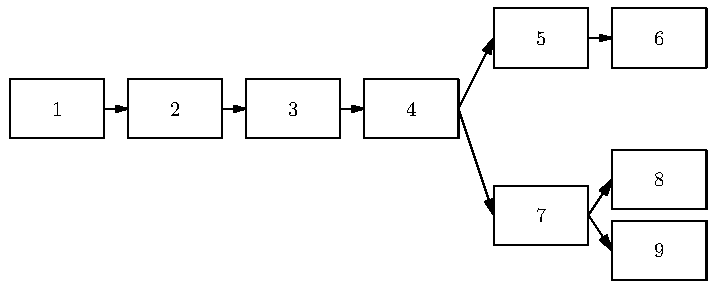
\includegraphics[scale=1.0]{structure.pdf}\end{SCentered}

\Ssubsectionstarx{用法}{用法}\label{t:x28part_x22pfx2dusex22x29}

本书在本科生和研究生课程中均已使用,也已在职业程序员的持续教育课程中使用。我们假
定的背景知识有数据结构,过程式语言(如C、C++、Java)和 Scheme、ML、Python 或
Haskell 的编程经验。

习题是文本的重要部分,散见于各处。它们难易有别,简单者,理解相关材料便轻而易举
(标为 \texMathInline{\textnormal{[}{\star}\textnormal{]}});困难者,需要花费大量思考和编程工作(标为
\texMathInline{\textnormal{[}{\star}{\star}{\star}\textnormal{]}})。大量关于应用,历史以及理论的材料潜藏其间。我们建议读一读
每道习题,想一想如何解决它们。虽然我们用 Scheme 编写解释程序和转换系统,任何支持
一等过程和赋值的语言(ML、Common Lisp、Python、Ruby等等)都足以完成本书练习。

\begin{EoplExercise}\label{t:x28elem_x22ex0x2e1x22x29}\texMathInline{\textnormal{[}{\star}\textnormal{]}}\mbox{\hphantom{\Scribtexttt{x}}}我们常说“某语言具有某性质”。为每种说法找出一种或多
种具有该性质的语言,以及一种或多种不具有该性质的语言。请随意搜索这些信息,不拘
任何编程语言的介绍性书籍(比如 Scott(2005),Sebesta (2007),或者 Pratt \&
Zelkowitz(2001))。\hspace*{\fill}\\\end{EoplExercise}

这是本实践性的书:本书讨论的一切都可在通常的大学课程限度内完成。因为函数式语言的
抽象特性尤其适合这类编程,我们可以写出强大的语言处理系统,既简洁,又能以适当的努
力掌握。

网站由出版社提供,包含本书所有解释器和分析器的完整 Scheme 代码。代码用 PLT
Scheme 写成。\NoteBox{\NoteContent{本书网站已迁移至 \href{http://www.eopl3.com}{\Snolinkurl{http://www.eopl3.com}},代码改用 Racket
实现,网址为 \href{https://github.com/mwand/eopl3}{\Snolinkurl{https://github.com/mwand/eopl3}}。{---}{---}\emph{译注}}}我们选择这种
Scheme 实现,是因为它的模块系统和编程环境对学生助益良多。代码多半兼容于
R\textsuper{5}RS,当能轻易移植到任何功能完整的 Scheme 实现。

\sectionNewpage

\Ssectionstarx{致谢}{致谢}\label{t:x28part_x22awkx22x29}

感谢无数同事同学,他们使用和评论了本书的前两版,又为第三版的漫长构思提供了无价帮
助。特别感激以下诸君的贡献,对他们我们深表谢忱。Oliver Danvy 鼓励我们思考一阶组
合式续文传递算法,并提出了一些饶有趣味的练习。Matthias Felleisen 切中肯綮的分析
改善了一些章节的设计。Amr Sabry 提出了许多有用的建议,在\ChapRefLocal{t:x28part_x22oacx22x29}{9}{对象和类}的草稿中发现
了至少一处极难察觉的问题。Benjamin Pierce 自使用本书第一版授课以来提出了一系列深
入见解,其中大半已为我们采用。Gary Leavens 对第二版的初稿提出了极为细致而珍贵的
评论,包括许多详细的修改建议。Stephanie Weirich 在本书第二版\ChapRefLocal{t:x28part_x22typesx22x29}{7}{类型}的类型
推导代码中发现了一个不易察觉的问题。Ryan Newton 除了阅读\ChapRefLocal{t:x28part_x22dax22x29}{2}{数据抽象}草稿之外,又
承担了一个艰巨任务:为该版的每道练习题推荐难度等级。Chung{-}chieh Shan 从第三版初
稿开始授课,提供了大量有益的评论。

Kevin Millikin、Arthur Lee、Roger Kirchner、Max Hailperin 和 Erik Hilsdale 使用
了第二版初稿。Will Clinger、Will Byrd、Joe Near 和 Kyle Blocher 使用了本版手稿。
他们的评论弥足珍贵。Ron Garcia、Matthew Flatt、Shriram Krishnamurthi、Steve Ganz、
Gregor Kiczales、Marlene Miller、Galen Williamson、Dipanwita Sarkar、Steven
Bogaerts、Albert Rossi、Craig Citro、Christopher Dutchyn、Jeremy Siek 和 Neil
Ching 也认真阅读并做了评论。

尤其感谢这几位对本书的帮助。感谢 Neil Ching 编制了索引。在我们尝试设计
\Scribtexttt{define{-}datatype} 和 \Scribtexttt{cases} 语法扩展时,Jonathan Sobel 和 Erik Hilsdale
完成了一些原型实现,贡献了很多想法。程序语言小组,尤其是 Matthias Felleisen、
Matthew Flatt、Robby Findler 和 Shriram Krishnamurthi,热心帮忙兼容他们的
DrScheme 系统。Kent Dybvig 开发了极为高效和健壮的 Chez Scheme 实现,本书作者已使
用多年。Will Byrd 在整个过程中都提供了无价帮助。Matthias Felleisen 强烈推荐我们
兼容 DrScheme 的模块系统,这在位于 \href{http://www.eopl3.com}{\Snolinkurl{http://www.eopl3.com}} 的实现中显而易见。

特别值得一提的是体贴和关心我们进度的人。George Springer 和 Larry Finkelstein 提
供了无价支持。特别感谢 Bob Prior,我们 MIT 出版社的优秀编辑,是他鼓励我们攻下本
版的写作。同样感谢 Bob 的继任 Ada Brunstein,帮我们流畅过渡到新的编辑。印第安纳
大学信息学院和东北大学计算机信息科学学院为我们进行这一工程创造了环境。Mary
Friedman 在数周的写作谈话中热情招待,大大加快了我们的进程。

我们感谢 Christopher T. Haynes 在前两版中的合作。很遗憾,他已志不在此,没有继续
同我们参与本版的编写。

最后,感谢我们的家人,包容我们写作本书时的热情。谢谢你,Rob、Shannon、Rachel、
Sara,还有 Mary;谢谢你,Rebecca 和 Joshua,Jennifer 和 Stephen,Joshua 和
Georgia,还有 Barbara。

本版筹备良久,我们可能忽视了一路帮助过我们的人。我们为任何忽视道歉。您总在书中看
到这样的话,可能会奇怪为什么有人会这样写。忽视了别人,你当然感到抱歉。但是,当你
有了一众帮手(得一个村子才装得下),你确实有种责任感:任何人都不容忽视。所以,如
果您被忽视了,我们深表歉意。\hspace*{\fill}\\

\Sright{{---}{---} D.P.F,M.W.}

\mainmatter{}

\sectionNewpage

\Ssection{归纳式数据集}{归纳式数据集}\label{t:x28part_x22isdx22x29}



解释器与检查器一类的程序是编程语言处理器的核心,本章介绍写这些用到的基本编程工具。

因为编程语言的语法通常为嵌套或者树状结构,递归将是我们的主要技巧。
\SecRefLocal{t:x28part_x22s1x2e1x22x29}{1.1}{递推定义的数据}和\SecRefLocal{t:x28part_x22s1x2e2x22x29}{1.2}{推导递归程序}介绍归纳定义数据结构的方法,并展示如何用这类定义指导
递归程序的编写。\SecRefLocal{t:x28part_x22s1x2e3x22x29}{1.3}{辅助过程和上下文参数}展示如何将这些技巧推广到更为复杂的程序。本章以大量
练习作结。这些练习是本章的核心。欲掌握本书余下部分依赖的递归编程技巧,得自它们的
经验不可或缺。

\Ssubsection{递推定义的数据}{递推定义的数据}\label{t:x28part_x22s1x2e1x22x29}

\index{dzi4tui1shu4ju4lei4xing2@递推数据类型!dzing4yi4@定义|(idxdecorator{}{}}
编写过程代码时,必须明确知道什么样的值能作为过程的参数,什么样的值是过程的合法返
回值。这些值的集合通常很复杂。本节介绍定义值集合的形式化技术。

\Ssubsubsection{归纳定义法}{归纳定义法}\label{t:x28part_x22s1x2e1x2e1x22x29}

\index{gzui1na4shi4ding4yi4@归纳式定义|(idxdecorator{}{}}
归纳定义法是定义值集合的有效方法。为解释这一方法,我们用它来描述自然数 \texMathInline{N =
{0,1,2,...}} 的某一子集 \texMathInline{S}。

\begin{EoplDefinition}\label{t:x28elem_x22d1x2e1x2e1x22x29}\mbox{\hphantom{\Scribtexttt{x}}}\index{zzi4ding3xiang4xia4ding4yi4@自顶向下定义|idxdecorator{}{}}
自然数 \texMathInline{n} 属于 \texMathInline{S},当且仅当:
 

\noindent \begin{enumerate}\atItemizeStart

\item \texMathInline{n = 0},或

\item \texMathInline{n - 3 \in S}\end{enumerate}\end{EoplDefinition}

来看看如何用这一定义判断哪些自然数属于 \texMathInline{S}。已知 \texMathInline{0 \in S},因此 \texMathInline{3 \in S},
因为 \texMathInline{(3 - 3) = 0},且 \texMathInline{0 \in S}。同样地,\texMathInline{6 \in S},因为 \texMathInline{(6 - 3) = 3},
且 \texMathInline{3 \in S}。依此类推,可得结论:所有 \texMathInline{3} 的整数倍都属于 \texMathInline{S}。

其他自然数呢?\texMathInline{1 \in S} 吗?已知 \texMathInline{1 \ne 0},所以条件一不满足。此外,\texMathInline{(1 -
3) = -2},不是自然数,故不是 \texMathInline{S} 的元素,因此条件二不满足。因为 \texMathInline{1} 不满足任
一条件,所以 \texMathInline{1 \notin S}。同样地,\texMathInline{2 \notin S}。\texMathInline{4}呢?仅当 \texMathInline{1 \in S}
时 \texMathInline{4 \in S}。但 \texMathInline{1 \notin S},所以 \texMathInline{4 \notin S}。同理可得,如果 \texMathInline{n} 是
自然数且不是 \texMathInline{3} 的整数倍,则 \texMathInline{n \notin S}。

据此推论,可得 \texMathInline{S} 是 \texMathInline{3} 的整数倍自然数集合。

可以用该定义编写一个函数,判断一个自然数 \texMathInline{n} 是否属于 \texMathInline{S}。

\begin{EoplCodeInset}\begin{SCodeFlow}\begin{RktBlk}\begin{SingleColumn}\index{inS@\textbf{\Scribtexttt{is{-}S{\hbox{\texttt{?}}}}}|idxdecorator{}{}}

\textbf{\Scribtexttt{in{-}S{\hbox{\texttt{?}}}}} : \texMathInline{\mathit{N} \to \mathit{Bool}}

\textbf{用法} : \Scribtexttt{(in{-}S{\hbox{\texttt{?}}} n) = \#t 若 n 属于 S,否则 \#f}

\RktPn{(}\RktSym{define}\mbox{\hphantom{\Scribtexttt{x}}}\RktSym{in{-}S{\hbox{\texttt{?}}}}

\mbox{\hphantom{\Scribtexttt{xx}}}\RktPn{(}\RktSym{lambda}\mbox{\hphantom{\Scribtexttt{x}}}\RktPn{(}\RktSym{n}\RktPn{)}

\mbox{\hphantom{\Scribtexttt{xxxx}}}\RktPn{(}\RktSym{if}\mbox{\hphantom{\Scribtexttt{x}}}\RktPn{(}\RktSym{zero{\hbox{\texttt{?}}}}\mbox{\hphantom{\Scribtexttt{x}}}\RktSym{n}\RktPn{)}\mbox{\hphantom{\Scribtexttt{x}}}\RktVal{\#t}

\mbox{\hphantom{\Scribtexttt{xxxxxxxx}}}\RktPn{(}\RktSym{if}\mbox{\hphantom{\Scribtexttt{x}}}\RktPn{(}\RktSym{{\Stttextmore}=}\mbox{\hphantom{\Scribtexttt{x}}}\RktPn{(}\RktSym{\mbox{{-}}}\mbox{\hphantom{\Scribtexttt{x}}}\RktSym{n}\mbox{\hphantom{\Scribtexttt{x}}}\RktVal{3}\RktPn{)}\mbox{\hphantom{\Scribtexttt{x}}}\RktVal{0}\RktPn{)}

\mbox{\hphantom{\Scribtexttt{xxxxxxxxxxxx}}}\RktPn{(}\RktSym{in{-}S{\hbox{\texttt{?}}}}\mbox{\hphantom{\Scribtexttt{x}}}\RktPn{(}\RktSym{\mbox{{-}}}\mbox{\hphantom{\Scribtexttt{x}}}\RktSym{n}\mbox{\hphantom{\Scribtexttt{x}}}\RktVal{3}\RktPn{)}\RktPn{)}

\mbox{\hphantom{\Scribtexttt{xxxxxxxxxxxx}}}\RktVal{\#f}\RktPn{)}\RktPn{)}\RktPn{)}\RktPn{)}\end{SingleColumn}\end{RktBlk}\end{SCodeFlow}\end{EoplCodeInset}

这里根据定义,我们用Scheme编写了一个递归过程。符号 \RktSym{in{-}S{\hbox{\texttt{?}}}}\Scribtexttt{ }\RktSym{{\hbox{\texttt{:}}}}\Scribtexttt{ }\texMathInline{\mathit{N} \to \mathit{Bool}} 是一条注释,称为该函数
\index{hze2yue1@合约|idxdecorator{}{}}
的\emph{合约} (\emph{contract})。它表示 \RktSym{in{-}S{\hbox{\texttt{?}}}} 应为一过程,取一自然数,产生一
布尔值。这样的注释对阅读和编写代码很有帮助。

要判断是否 \texMathInline{n \in S},先判断是否 \texMathInline{n = 0}。如果是,那么答案为真。否则,判断是
否 \texMathInline{n - 3 \in S}。欲知此,首先判断是否 \texMathInline{(n - 3) \geqslant 0}。如果是,那么可
以用我们的过程判断它是否属于 \texMathInline{S}。如果不是,那么 \texMathInline{n} 不可能属于 \texMathInline{S}。

\texMathInline{S} 又能够定义为:

\begin{EoplDefinition}\label{t:x28elem_x22d1x2e1x2e2x22x29}\mbox{\hphantom{\Scribtexttt{x}}}集合 \texMathInline{S} 为 \texMathInline{N} 所包含的集合中,满足如下两条性质的最小集合:\index{zzui4xiao3ji2he2@最小集合|idxdecorator{}{}}

\begin{enumerate}\atItemizeStart

\item \texMathInline{0 \in S},且

\item 若 \texMathInline{n \in S},则 \texMathInline{n + 3 \in S}。\end{enumerate}\end{EoplDefinition}

“最小集合”是指该集合满足性质 1 和 2,并且是其他任何
满足性质 1 和 2 的集合的子集。易知只能有一个这样的集合:如果 \texMathInline{S_1} 和 \texMathInline{S_2}
都满足性质 1 和 2,并且都为最小,那么 \texMathInline{S_1 \subseteq S_2}(因为 \texMathInline{S_1} 最小)
且 \texMathInline{S_2 \subseteq S_1}(因为 \texMathInline{S_2} 最小),因此 \texMathInline{S_1 = S_2}。之所以需要这
一额外条件,是因为否则的话将有许多集合满足其他两个条件(见)。

该定义还能表示为:

\texMathDisplay{\infer{0 \in S}{}}

\texMathDisplay{\infer{(n + 3) \in S}{n \in S}}

\index{tzui1li3gui1ze2@推理规则|idxdecorator{}{}}
这只是前一定义的简便表示。每个条目称为一条\emph{推理规则} (\emph{rule of inference}),
或称\emph{规则} (\emph{rule});水平线读作“若{-}则”。线上部分
称作\emph{假设} (\emph{hypothesis})或者\index{qzian2jian4@前件|idxdecorator{}{}}\emph{前件} (\emph{antecedent});
\index{jzie2lun4@结论|idxdecorator{}{}}
\index{hzou4jian4@后件|idxdecorator{}{}}
\index{jzia3she4@假设|idxdecorator{}{}}
线下部分称作\emph{结论} (\emph{conclusion}) 或者\emph{后件} (\emph{consequent})。罗列两个或
更多假设时,它们以隐含的“与”连接(见)。
不含假设的规则称作\index{gzong1li3@公理|idxdecorator{}{}}\emph{公理} (\emph{axiom})。写公理时通常不加水平
线,如:

\texMathDisplay{0 \in S}

该规则意为,自然数 \texMathInline{n} 属于 \texMathInline{S},当且仅当能用有限次推理规则,从公理推得陈述
“\texMathInline{n \in S}”。这一解释自然使 \texMathInline{S} 成为闭合于该规则
的最小集合。

\index{zzi4di3xiang4shang4ding4yi4@自底向上定义|idxdecorator{}{}}
\index{zzi4ding3xiang4xia4ding4yi4@自顶向下定义|idxdecorator{}{}}
这些定义意思相同。我们把版本一称作\emph{自顶向下} (\emph{top{-}down}) 的定义,版本二
称作\emph{自底向上} (\emph{bottom{-}up}) 的定义,版本三称作\emph{推理规则}定义。
\index{tzui1li3gui1ze2ding4yi4@推理规则定义|idxdecorator{}{}}

再来看几个运用这些的例子。

\index{zzheng3shu4lie4biao3@整数列表 (\texMathInline{\mathit{List\mbox{-}of\mbox{-}Int}})|(idxdecorator{}{}}


\noindent \begin{EoplDefinition}\label{t:x28elem_x22d1x2e1x2e3x22x29}\EoplDefinitionTitle{整数列表,自顶向下}Scheme列表是整数列表,当且仅当:


\noindent \begin{enumerate}\atItemizeStart

\item 列表为空,或

\item 列表为序对,首项为整数,余项为整数列表。\end{enumerate}\end{EoplDefinition}

我们用 \texMathInline{\mathit{Int}} 表示所有整数的集合,用 \texMathInline{\mathit{List\mbox{-}of\mbox{-}Int}} 表示所有整数列表的集合。

\begin{EoplDefinition}\label{t:x28elem_x22d1x2e1x2e4x22x29}\EoplDefinitionTitle{整数列表,自底向上}集合\texMathInline{\mathit{List\mbox{-}of\mbox{-}Int}}是满足如下两条性质的最小Scheme列表集合:

\begin{enumerate}\atItemizeStart

\item \texMathInline{\textnormal{\Scribtexttt{()}} \in \texMathInline{\mathit{List\mbox{-}of\mbox{-}Int}}},或

\item 若 \texMathInline{n \in \mathit{Int}} 且 \texMathInline{l \in \texMathInline{\mathit{List\mbox{-}of\mbox{-}Int}}},则
\texMathInline{\textnormal{\texttt{(}}n\phantom{x}.\phantom{x}l\textnormal{\texttt{)}} \in
\texMathInline{\mathit{List\mbox{-}of\mbox{-}Int}}}。\end{enumerate}\end{EoplDefinition}

\index{dzian3zhui4biao3shi4fa3@点缀表示法|idxdecorator{}{}}
这里,我们用中缀“\Scribtexttt{{\hbox{\texttt{.}}}}”代表 Scheme 中 \Scribtexttt{cons} 操
作的结果。式子 \Scribtexttt{(}\texMathInline{n}\Scribtexttt{ {\hbox{\texttt{.}}} }\texMathInline{l}\Scribtexttt{)} 代表 Scheme 序对的首项为 \texMathInline{n},余项为 \texMathInline{l}。

\begin{EoplDefinition}\label{t:x28elem_x22d1x2e1x2e5x22x29}\EoplDefinitionTitle{整数列表,推理规则}

\noindent \begin{NormalFont}\index{tzui1li3gui1ze2ding4yi4@推理规则定义|idxdecorator{}{}}
\texMathDisplay{\infer{\Scribtexttt{()} \in \texMathInline{\mathit{List\mbox{-}of\mbox{-}Int}}}{}}

\texMathDisplay{\infer{\Scribtexttt{(}\texMathInline{n}\Scribtexttt{ {\hbox{\texttt{.}}} }\texMathInline{l}\Scribtexttt{)} \in \texMathInline{\mathit{List\mbox{-}of\mbox{-}Int}}}{n \in \mathit{Int} & l \in
\texMathInline{\mathit{List\mbox{-}of\mbox{-}Int}}}}\end{NormalFont}

\noindent \index{zzheng3shu4lie4biao3@整数列表 (\texMathInline{\mathit{List\mbox{-}of\mbox{-}Int}})|)idxdecorator{}{}}\end{EoplDefinition}

这三个定义等价。来看看如何用它们生成一些 \texMathInline{\mathit{List\mbox{-}of\mbox{-}Int}} 的元素。

\begin{enumerate}\atItemizeStart

\item 由 的性质 1 或 的规则 1,
\Scribtexttt{()} 是整数列表。

\item 由 的性质 2,\Scribtexttt{(14 {\hbox{\texttt{.}}} ())} 是整数列表。因为
\Scribtexttt{14} 是整数,\Scribtexttt{()} 是整数列表。写成 \texMathInline{\mathit{List\mbox{-}of\mbox{-}Int}} 规则二的形式,
就是

\texMathDisplay{\infer{\Scribtexttt{(14 {\hbox{\texttt{.}}} ())} \in \texMathInline{\mathit{List\mbox{-}of\mbox{-}Int}}} {\Scribtexttt{14} \in \mathit{Int}
& \Scribtexttt{()} \in \texMathInline{\mathit{List\mbox{-}of\mbox{-}Int}}}}

\item 由 的性质 2,\Scribtexttt{(3 {\hbox{\texttt{.}}} (14 {\hbox{\texttt{.}}} ()))} 是整数列表。因为
\Scribtexttt{3} 是整数,\Scribtexttt{(14 {\hbox{\texttt{.}}} ())} 是整数列表。仍写成\texMathInline{\mathit{List\mbox{-}of\mbox{-}Int}} 规则二的
形式,是

\texMathDisplay{\infer{\Scribtexttt{(3 {\hbox{\texttt{.}}} (14 {\hbox{\texttt{.}}} ()))} \in \texMathInline{\mathit{List\mbox{-}of\mbox{-}Int}}} {\Scribtexttt{3} \in
\mathit{Int} & \Scribtexttt{(14 {\hbox{\texttt{.}}} ())} \in \texMathInline{\mathit{List\mbox{-}of\mbox{-}Int}}}}

\item 由 的性质 2,\Scribtexttt{({-}7 {\hbox{\texttt{.}}} (3 {\hbox{\texttt{.}}} (14 {\hbox{\texttt{.}}} ())))} 是整数列
表。因为 \Scribtexttt{{-}7} 是整数,\Scribtexttt{(3 {\hbox{\texttt{.}}} (14 {\hbox{\texttt{.}}} ()))} 是整数列表。再次写成
\texMathInline{\mathit{List\mbox{-}of\mbox{-}Int}} 规则二的形式,是

\texMathDisplay{\infer{\hphantom{\texttt{x}}\Scribtexttt{({-}7 {\hbox{\texttt{.}}} (3 {\hbox{\texttt{.}}} (14 {\hbox{\texttt{.}}} ())))} \in \texMathInline{\mathit{List\mbox{-}of\mbox{-}Int}}\hphantom{\texttt{x}}}
      {\Scribtexttt{{-}7} \in \mathit{Int} & \Scribtexttt{(3 {\hbox{\texttt{.}}} (14 {\hbox{\texttt{.}}} ()))}\in \texMathInline{\mathit{List\mbox{-}of\mbox{-}Int}}}}

\item 不按照这种方式得到的都不是整数列表。\end{enumerate}

改句点表示法为列表表示法,可知 \Scribtexttt{()}、 \Scribtexttt{(14)}、 \Scribtexttt{(3 14)} 以及 \Scribtexttt{({-}7 3
14)} 都是 \texMathInline{\mathit{List\mbox{-}of\mbox{-}Int}} 的元素。

还可以结合各条规则来证明 \texMathInline{\Scribtexttt{({-}7 {\hbox{\texttt{.}}} (3 {\hbox{\texttt{.}}} (14 {\hbox{\texttt{.}}} ())))} \in \texMathInline{\mathit{List\mbox{-}of\mbox{-}Int}}},
以见出整个推理过程。下面的树状图叫做\label{t:x28elem_x22derivx2dtreex22x29}\emph{推导} (\emph{derivation})
或\emph{推理树} (\emph{deduction tree})。
\index{tzui1dao3@推导|idxdecorator{}{}}
\index{tzui1li3shu4@推理树|idxdecorator{}{}}

\texMathDisplay{\infer{\hphantom{\texttt{xx}}\Scribtexttt{({-}7 {\hbox{\texttt{.}}} (3 {\hbox{\texttt{.}}} (14 {\hbox{\texttt{.}}} ())))} \in \texMathInline{\mathit{List\mbox{-}of\mbox{-}Int}}\hphantom{\texttt{xx}}}
      {\Scribtexttt{{-}7} \in \mathit{Int} \hphantom{\texttt{x}} &
       \infer{\hphantom{\texttt{x}}\Scribtexttt{(3 {\hbox{\texttt{.}}} (14 {\hbox{\texttt{.}}} ()))} \in \texMathInline{\mathit{List\mbox{-}of\mbox{-}Int}}\hphantom{\texttt{x}}}
             {\Scribtexttt{3} \in \mathit{Int} &
              \infer{\Scribtexttt{(14 {\hbox{\texttt{.}}} ())} \in \texMathInline{\mathit{List\mbox{-}of\mbox{-}Int}}}
                    {\Scribtexttt{14} \in \mathit{Int} & \Scribtexttt{()} \in \texMathInline{\mathit{List\mbox{-}of\mbox{-}Int}}}}
      }}
\index{gzui1na4shi4ding4yi4@归纳式定义|)idxdecorator{}{}}

\begin{EoplExercise}\label{t:x28elem_x22ex1x2e1x22x29}\texMathInline{\textnormal{[}{\star}\textnormal{]}}\mbox{\hphantom{\Scribtexttt{x}}}写出下列集合的归纳定义。以三种方式(自顶向下,自底向上,推理规则)写出每个定
义,并用你的规则推导出各集合的一些元素。

\begin{enumerate}\atItemizeStart

\item \Iidentity{$\{ 3n + 2 \mid n \in N \}$}

\item \Iidentity{$\{ 2n + 3m + 1 \mid n, m \in N \}$}

\item \Iidentity{$\{ (n, 2n + 1) \mid n \in N \}$}

\item \Iidentity{$\{ (n, n^2) \mid n \in N \}$}。不要在你的规则中使用平方。提示:想一想
方程 \Iidentity{$ (n + 1) ^ 2 = n ^ 2 + 2n + 1$}。\end{enumerate}\end{EoplExercise}

\begin{EoplExercise}\label{t:x28elem_x22ex1x2e2x22x29}\texMathInline{\textnormal{[}{\star}{\star}\textnormal{]}}\mbox{\hphantom{\Scribtexttt{x}}}下面的几对规则分别定义了什么集合?给出解释。

\begin{enumerate}\atItemizeStart

\item \Iidentity{$(0, 1) \in S \qquad \infer{(n + 1, k + 7) \in S}{(n, k) \in S}$}

\item \Iidentity{$(0, 1) \in S \qquad \infer{(n + 1, 2k) \in S}{(n, k) \in S}$}

\item \Iidentity{$(0, 0, 1) \in S \qquad \infer{(n + 1, j, i + j) \in S}{(n, i, j) \in S}$}

\item \Iidentity{$\text{[}\mathord{\star}\mathord{\star}\mathord{\star}\text{]}$}
\Iidentity{$\quad$} \Iidentity{$(0, 1, 0) \in S \qquad \infer{(n + 1, i + 2, i + j) \in S}{(n, i,
j) \in S}$}\end{enumerate}\end{EoplExercise}

\begin{EoplExercise}\label{t:x28elem_x22ex1x2e3x22x29}\texMathInline{\textnormal{[}{\star}\textnormal{]}}\mbox{\hphantom{\Scribtexttt{x}}}\index{zzui4xiao3ji2he2@最小集合|(idxdecorator{}{}}
找出自然数的子集 \Iidentity{$T$},满足 \Iidentity{$0 \in T$},且对任何 \Iidentity{$n \in T$},都有 \Iidentity{$n + 3
\in T$},但 \Iidentity{$T \neq S$},\Iidentity{$S$} 是由 给出的集合。
\index{zzui4xiao3ji2he2@最小集合|)idxdecorator{}{}}\end{EoplExercise}

\Ssubsubsection{语法定义法}{语法定义法}\label{t:x28part_x22s1x2e1x2e2x22x29}

\index{yzu3fa3@语法|(idxdecorator{}{}}
前述例子较为直观,但是不难想象,描述更复杂的数据类型会有多麻烦。为了方便,我们展
示如何用\emph{语法} (\emph{grammar}) 定义集合。语法通常用来指定字符串的集合,但也能用
来定义值的集合。

\index{zzheng3shu4lie4biao3@整数列表 (\texMathInline{\mathit{List\mbox{-}of\mbox{-}Int}})|(idxdecorator{}{}}
例如,集合 \texMathInline{\mathit{List\mbox{-}of\mbox{-}Int}} 可用语法定义为:

\begin{Small}\Iidentity{\begin{align*}\mathit{List\mbox{-}of\mbox{-}Int} &::= \Scribtexttt{()} \\[-3pt]
\mathit{List\mbox{-}of\mbox{-}Int} &::= \Scribtexttt{(}\Iidentity{\mathit{Int}}\Scribtexttt{ {\hbox{\texttt{.}}} }\Iidentity{\mathit{List\mbox{-}of\mbox{-}Int}}\Scribtexttt{)}\end{align*}}\end{Small}

这两条规则对应上述 中的两条性质。规则一是说空表属于
\texMathInline{\mathit{List\mbox{-}of\mbox{-}Int}};规则二是说,若 \texMathInline{n} 属于 \texMathInline{\mathit{Int}} 且 \texMathInline{l} 属于
\texMathInline{\mathit{List\mbox{-}of\mbox{-}Int}},则 \Scribtexttt{(}\texMathInline{n}\Scribtexttt{ {\hbox{\texttt{.}}} }\texMathInline{l}\Scribtexttt{)} 属于 \texMathInline{\mathit{List\mbox{-}of\mbox{-}Int}}。这些规则
叫做\emph{语法}。

来看看该定义的各个部分,其中有:

\begin{itemize}\atItemizeStart

\item \textbf{非终结符}。这些是所定义的集合名。本例中只定义了一个集合,但是通常,
可能会定义数个集合。这些集合有时称为\emph{句法类别} (\emph{syntactic category})。
\index{fzei1zhong1jie2fu2@非终结符|idxdecorator{}{}}
\index{jzu4fa3lei4bie2@句法类别|idxdecorator{}{}}

依照惯例,我们将非终结符和集合名的首字母大写,在文中提及它们的元素时,则
用小写。这要比听起来容易。例如, \texMathInline{\mathit{Expression}} 是非终结符,但
我们写作 \texMathInline{e \in \mathit{Expression}} 或 “\texMathInline{e} 是一个
expression”。

另一常见写法,名叫\emph{巴科斯{-}诺尔范
式} (\emph{Backus{-}Naur Form})\index{bza1ke1si1nuo4er3fan4shi4BNF@巴科斯{-}诺尔范式 (BNF)|idxdecorator{}{}} 或\emph{BNF},是在词周围加
尖括号,如\texMathInline{\langle}expression\texMathInline{\rangle}。

\item \textbf{终结符}。这些是集合外在表示中的字符,在本例中,是
“\Scribtexttt{{\hbox{\texttt{.}}}}”、
“\Scribtexttt{(}”和
“\Scribtexttt{)}”。这些常用打字机字体写出,如
\Scribtexttt{lambda}。\index{zzhong1jie2fu2@终结符|idxdecorator{}{}}

\item \textbf{生成式}。规则叫做\emph{生成式} (\emph{production})。
\index{yzu3fa3sheng1cheng2shi4@语法生成式|idxdecorator{}{}}每个生成式的左边是一个非终结符,右边
包含终结符和非终结符。左右两边通常用符号 \texMathInline{::=}分隔,读作\emph{是}
或\emph{可以是}。式子右边用其他句法类别和\emph{终结符}(如左括号、
右括号和句点)指定一种方法,用以构建当前句法类别的元素。\end{itemize}

如果某些句法类别的含义在上下文中足够清晰,在生成式中提到它们时通常不作定义,如
\texMathInline{\mathit{Int}}。

语法常常简写。当一个生成式的左边与前一生成式相同时,一般会略去。根据这一惯例,我
们的语法可以写作

\begin{Small}\Iidentity{\begin{align*}\mathit{List\mbox{-}of\mbox{-}Int} &::= \Scribtexttt{()} \\[-3pt]
                   &::= \Scribtexttt{(}\Iidentity{\mathit{Int}}\Scribtexttt{ {\hbox{\texttt{.}}} }\Iidentity{\mathit{List\mbox{-}of\mbox{-}Int}}\Scribtexttt{)}\end{align*}}\end{Small}

给同一句法类别编写一组规则时,也可以只写一次 \texMathInline{::=} 和左边内容,随后的各个右边
内容用特殊符号“\texMathInline{\mid}”(竖线,读作\emph{或}\index{hzuo4@或|idxdecorator{}{}})
分隔。用“\texMathInline{\mid}”,\texMathInline{\mathit{List\mbox{-}of\mbox{-}Int}} 的语法可写成:

\texMathDisplay{\texMathInline{\mathit{List\mbox{-}of\mbox{-}Int}} ::= \Scribtexttt{()} \texMathDisplay{\mid} \Scribtexttt{(}\texMathInline{\mathit{Int}}\Scribtexttt{ {\hbox{\texttt{.}}} }\texMathInline{\mathit{List\mbox{-}of\mbox{-}Int}}\Scribtexttt{)}}
\index{zzheng3shu4lie4biao3@整数列表 (\texMathInline{\mathit{List\mbox{-}of\mbox{-}Int}})|)idxdecorator{}{}}

\index{kze4lai2ni2xing1hao4bi4bao1@克莱尼星号(闭包)|idxdecorator{}{}}
另一种简写是\label{t:x28elem_x22kleenex2dstarx22x29}\emph{克莱尼星号} (\emph{Kleene Star}),写作
\texMathInline{\{...\}^*}。当它出现在右边时,表示一个序列,由任意多个花括号之间的内容组成。
用克莱尼星号,\texMathInline{\mathit{List\mbox{-}of\mbox{-}Int}} 的定义可以简写为

\texMathDisplay{\texMathInline{\mathit{List\mbox{-}of\mbox{-}Int}} ::= \Scribtexttt{(}\texMathInline{\{\mathit{Int}\}^*}\Scribtexttt{)}}

这也包含没有任何内容的情况。如果内容出现 0 次,得到的是空字符串。

\index{kze4lai2ni2jia1hao4@克莱尼加号|idxdecorator{}{}}
星号的变体是\emph{克莱尼加号} (\emph{Kleene Plus}) \texMathInline{\{...\}^+},表示一个或多个内容的
序列。把上例中的 \texMathInline{^*} 换成 \texMathInline{^+},定义的句法类别是非空整数列表。

\index{fzen1ge2biao3biao3shi4fa3@分隔表表示法|(idxdecorator{}{}}
星号的另一变体是\emph{分隔表} (\emph{separated list}) 表示法。例如,
\texMathInline{\mathit{Int}^{*(c)}} 表示一个序列,包含任意数量的非终结符 \texMathInline{\mathit{Int}} 元素,以非
空字符序列 \texMathInline{c} 分隔。这也包含没有元素的情况。如果有 0 个元素,得到的是空字符串。
例如,\texMathInline{\mathit{Int}^{*(,)}} 包含字符串

\begin{Subflow}\begin{EoplCodeInset}\begin{SVerbatim}\begin{SingleColumn}\Scribtexttt{8}

\Scribtexttt{14, 12}

\Scribtexttt{7, 3, 14, 16}\end{SingleColumn}\end{SVerbatim}\end{EoplCodeInset}

\texMathInline{\mathit{Int}^{*(;)}} 包含字符串

\begin{EoplCodeInset}\begin{SVerbatim}\begin{SingleColumn}\Scribtexttt{8}

\Scribtexttt{14; 12}

\Scribtexttt{7; 3; 14; 16}\end{SingleColumn}\end{SVerbatim}

\noindent \index{fzen1ge2biao3biao3shi4fa3@分隔表表示法|)idxdecorator{}{}}\end{EoplCodeInset}\end{Subflow}

这些简写不是必需的,总能够不用它们重写语法。

\index{jzu4fa3tui1dao3@句法推导|idxdecorator{}{}}
\index{jzu4fa3tui1dao3@句法推导|idxdecorator{}{}}
对由语法定义的集合,可以用\emph{句法推导} (\emph{syntactic derivation}) 证明给定值是其
元素。这样的推导从集合对应的非终结符开始,在由箭头\texMathInline{\Rightarrow} 指示的每一步中,
如果非终结符对应的句法类别未做定义,则将其代换为该类别的已知元素,否则代换为对应
规则右边的内容。例如,前述证明“\Scribtexttt{(14 {\hbox{\texttt{.}}} ())} 是整数列表
”,可以用句法推导化为

\begin{Small}\Iidentity{\begin{align*}\mathit{List\mbox{-}of\mbox{-}Int} &\Rightarrow \Scribtexttt{(}\Iidentity{\mathit{Int}}\Scribtexttt{ {\hbox{\texttt{.}}} }\Iidentity{\mathit{List\mbox{-}of\mbox{-}Int}}\Scribtexttt{)} \\[-3pt]
                   &\Rightarrow \Scribtexttt{(14 {\hbox{\texttt{.}}} }\Iidentity{\mathit{List\mbox{-}of\mbox{-}Int}}\Scribtexttt{)} \\[-3pt]
                   &\Rightarrow \Scribtexttt{(14 {\hbox{\texttt{.}}} ())}\end{align*}}\end{Small}

非终结符的替换顺序无关紧要,所以 \Scribtexttt{(14 {\hbox{\texttt{.}}} ())} 的推导也可以写成:

\begin{Small}\Iidentity{\begin{align*}\mathit{List\mbox{-}of\mbox{-}Int} &\Rightarrow \Scribtexttt{(}\Iidentity{\mathit{Int}}\Scribtexttt{ {\hbox{\texttt{.}}} }\Iidentity{\mathit{List\mbox{-}of\mbox{-}Int}}\Scribtexttt{)} \\[-3pt]
                   &\Rightarrow \Scribtexttt{(}\Iidentity{\mathit{Int}}\Scribtexttt{ {\hbox{\texttt{.}}} ())} \\[-3pt]
                   &\Rightarrow \Scribtexttt{(14 {\hbox{\texttt{.}}} ())}\end{align*}}\end{Small}

\begin{EoplExercise}\label{t:x28elem_x22ex1x2e4x22x29}\texMathInline{\textnormal{[}{\star}\textnormal{]}}\mbox{\hphantom{\Scribtexttt{x}}}写出从 \Iidentity{$\mathit{List\mbox{-}of\mbox{-}Int}$} 到 \Scribtexttt{({-}7 {\hbox{\texttt{.}}} (3 {\hbox{\texttt{.}}} (14 ())))} 的推导。\hspace*{\fill}\\\end{EoplExercise}

再来看一些有用集合的定义。

\begin{enumerate}\atItemizeStart

\item \index{Sexp@S{-}exp (\texMathInline{\mathit{S\mbox{-}exp}})|(idxdecorator{}{}}
\index{Slist@S{-}list (\texMathInline{\mathit{S\mbox{-}list}})|(idxdecorator{}{}}
许多符号操作过程用于处理只包含符号和具有类似限制的列表。我们把这些叫做
\Scribtexttt{s{-}list},定义如下:

\begin{EoplDefinition}\label{t:x28elem_x22d1x2e1x2e6x22x29}\EoplDefinitionTitle{s{-}list,s{-}exp}

\noindent \begin{NormalFont}\begin{Small}\Iidentity{\begin{align*}\mathit{S\mbox{-}list} &::= \Scribtexttt{(}\Iidentity{\{\mathit{S\mbox{-}exp}\}^*}\Scribtexttt{)} \\[-3pt]
\mathit{S\mbox{-}exp} &::= \mathit{Symbol} \mid \mathit{S\mbox{-}list}\end{align*}}\end{Small}\end{NormalFont}\end{EoplDefinition}

\label{t:x28elem_x22sx2dlistx22x29}s{-}list 是 s{-}exp 的列表,s{-}exp 或者是 s{-}list,或者是一个符号。
这里是一些 s{-}list。

\begin{EoplCodeInset}\begin{SVerbatim}\begin{SingleColumn}\Scribtexttt{(a b c)}

\Scribtexttt{(an (((s{-}list)) (with () lots) ((of) nesting)))}\end{SingleColumn}\end{SVerbatim}\end{EoplCodeInset}

有时也使用更宽松的 s{-}list 定义,既允许整数,也允许符号。
\index{Sexp@S{-}exp (\texMathInline{\mathit{S\mbox{-}exp}})|)idxdecorator{}{}}
\index{Slist@S{-}list (\texMathInline{\mathit{S\mbox{-}list}})|)idxdecorator{}{}}

\item 使用三元素列表表示内部节点,则以数值为叶子,以符号标示内部节点的二叉树可
用语法表示为:
\index{ezr4cha1shu4@二叉树 (\texMathInline{\mathit{Bintree}})|idxdecorator{}{}}

\begin{EoplDefinition}\label{t:x28elem_x22d1x2e1x2e7x22x29}\EoplDefinitionTitle{二叉树}

\noindent \begin{NormalFont}\begin{Small}\texMathDisplay{\mathit{Bintree} ::= \mathit{Int} \mid \Scribtexttt{(}\texMathInline{\mathit{Symbol}}\Scribtexttt{ }\texMathInline{\mathit{Bintree}}\Scribtexttt{ }\texMathInline{\mathit{Bintree}}\Scribtexttt{)}}\end{Small}\end{NormalFont}\end{EoplDefinition}

这是此类树的几个例子:

\begin{EoplCodeInset}\begin{SVerbatim}\begin{SingleColumn}\Scribtexttt{1}

\Scribtexttt{2}

\Scribtexttt{(foo 1 2)}

\Scribtexttt{(bar 1 (foo 1 2))}

\Scribtexttt{(baz}

\Scribtexttt{}\mbox{\hphantom{\Scribtexttt{x}}}\Scribtexttt{(bar 1 (foo 1 2))}

\Scribtexttt{}\mbox{\hphantom{\Scribtexttt{x}}}\Scribtexttt{(biz 4 5))}\end{SingleColumn}\end{SVerbatim}\end{EoplCodeInset}

\item \emph{lambda 演算} (\emph{lambda calculus}) 是一种简单语言,常用于研究编程语言
理论。这一语言只包含变量引用,单参数过程,以及过程调用,可用语法定义为:
\index{Lambdayzan3suan4@Lambda 演算|idxdecorator{}{}}

\begin{EoplDefinition}\label{t:x28elem_x22d1x2e1x2e8x22x29}\EoplDefinitionTitle{lambda 演算}\index{Lambdabziao3da2shi4LcExp@Lambda 表达式 (LcExp)|(idxdecorator{}{}}


\noindent \begin{NormalFont}\begin{Small}\Iidentity{\begin{align*}\mathit{LcExp} &::= \mathit{Identifier} \\[-3pt]
               &::= \Scribtexttt{(lambda (}\Iidentity{\mathit{Identifier}}\Scribtexttt{) }\Iidentity{\mathit{LcExp}}\Scribtexttt{)} \\[-3pt]
               &::= \Scribtexttt{(}\Iidentity{\mathit{LcExp}}\Scribtexttt{ }\Iidentity{\mathit{LcExp}}\Scribtexttt{)}\end{align*}}\end{Small}\end{NormalFont}

其中,identifier 是除 \NormalFont{\Scribtexttt{lambda}} 之外的任何符号。\end{EoplDefinition}

\index{bzang3ding4Binding@绑定 (Binding)!lambda@lambda|idxdecorator{}{}}
\index{bzang3ding4bian4liang4@绑定变量|idxdecorator{}{}}
\index{bzian4liang4@变量!bzang3ding4boundbian4liang4@绑定 (bound) 变量|idxdecorator{}{}}
第二个生成式中的 identifier 是 \Scribtexttt{lambda} 表达式主体内的变量名。这一变量叫做表
达式的\emph{绑定变量} (\emph{bound variable}),因为它绑定(或称捕获)主体内出现的任何
同名变量。出现在主体内的同名变量都指代这一个。
\index{Lambdabziao3da2shi4LcExp@Lambda 表达式 (LcExp)|)idxdecorator{}{}}

要明白这怎么用,考虑用算术操作符扩展的 lambda 演算。在这种语言里,

\begin{EoplCodeInset}\begin{SCodeFlow}\begin{RktBlk}\begin{SingleColumn}\RktPn{(}\RktSym{lambda}\RktMeta{}\mbox{\hphantom{\Scribtexttt{x}}}\RktMeta{}\RktPn{(}\RktSym{x}\RktPn{)}\RktMeta{}\mbox{\hphantom{\Scribtexttt{x}}}\RktMeta{}\RktPn{(}\RktSym{+}\RktMeta{}\mbox{\hphantom{\Scribtexttt{x}}}\RktMeta{}\RktSym{x}\RktMeta{}\mbox{\hphantom{\Scribtexttt{x}}}\RktMeta{}\RktVal{5}\RktPn{)}\RktPn{)}\RktMeta{}\end{SingleColumn}\end{RktBlk}\end{SCodeFlow}\end{EoplCodeInset}

是一表达式,\Scribtexttt{x} 是其绑定变量。这式子表示一个过程,把它的参数加5。因此,在

\begin{EoplCodeInset}\begin{SCodeFlow}\begin{RktBlk}\begin{SingleColumn}\RktPn{(}\RktPn{(}\RktSym{lambda}\RktMeta{}\mbox{\hphantom{\Scribtexttt{x}}}\RktMeta{}\RktPn{(}\RktSym{x}\RktPn{)}\RktMeta{}\mbox{\hphantom{\Scribtexttt{x}}}\RktMeta{}\RktPn{(}\RktSym{+}\RktMeta{}\mbox{\hphantom{\Scribtexttt{x}}}\RktMeta{}\RktSym{x}\RktMeta{}\mbox{\hphantom{\Scribtexttt{x}}}\RktMeta{}\RktVal{5}\RktPn{)}\RktPn{)}\RktMeta{}\mbox{\hphantom{\Scribtexttt{x}}}\RktMeta{}\RktPn{(}\RktSym{\mbox{{-}}}\RktMeta{}\mbox{\hphantom{\Scribtexttt{x}}}\RktMeta{}\RktSym{x}\RktMeta{}\mbox{\hphantom{\Scribtexttt{x}}}\RktMeta{}\RktVal{7}\RktPn{)}\RktPn{)}\RktMeta{}\end{SingleColumn}\end{RktBlk}\end{SCodeFlow}\end{EoplCodeInset}

中,最后一个出现的 \Scribtexttt{x} 不是指 \Scribtexttt{lambda} 表达式中绑定的 \Scribtexttt{x}。
\SecRefLocal{t:x28part_x22s1x2e2x2e4x22x29}{1.2.4}{\Scribtexttt{occurs{-}free{\hbox{\texttt{?}}}}}中介绍了 \Scribtexttt{occurs{-}free{\hbox{\texttt{?}}}},到时我们再讨论这个问题。

该语法定义 \texMathInline{\mathit{LcExp}} 的元素为 Scheme 值,因此很容易写出程序来处理它们。\end{enumerate}

\index{szhang4xia4wen2wu2guan1yu3fa3@上下文无关语法|idxdecorator{}{}}
这些语法叫做\emph{上下文无关} (\emph{context{-}free}) 语法,因为一条规则定义的句法类别可
以在任何引用它的上下文中使用。有时这不够严格。考虑\label{t:x28elem_x22bstx22x29}二叉搜索树。
其节点或者为空,或者包含一个整数和两棵子树
\index{ezr4cha1sou1suo3shu4@二叉搜索树 (\texMathInline{\mathit{Binary\mbox{-}search\mbox{-}tree}})|idxdecorator{}{}}
\texMathDisplay{\mathit{Binary\mbox{-}search\mbox{-}tree} ::= \Scribtexttt{()} \mid
\Scribtexttt{(}\texMathInline{\mathit{Int}}\Scribtexttt{ }\texMathInline{\mathit{Binary\mbox{-}search\mbox{-}tree}}\Scribtexttt{ }\texMathInline{\mathit{Binary\mbox{-}search\mbox{-}tree}}\Scribtexttt{)}}

这如实反映了每个节点的结构,但是忽略了二叉搜索树的一个要点:所有左子树的键值都小
于(或等于)当前节点,所有右子树的键值都大于当前节点。

\index{bzu4bian4shi4@不变式|(idxdecorator{}{}}
因为这条额外限制,从 \texMathInline{\mathit{Binary\mbox{-}search\mbox{-}tree}} 得出的句法推
导并不都是正确的二叉搜索树。要判定某个生成式能否用于特定的句法推导,必须检查生成
式用在哪种上下文。这种限制叫做\emph{上下文敏感
限制} (\emph{context{-}sensitive constraints}),或称\label{t:x28elem_x22invariantx22x29}\emph{不变式} (\emph{invariants})。
\index{szhang4xia4wen2min3gan3xian4zhi4@上下文敏感限制|(idxdecorator{}{}}

定义编程语言的语法也会产生上下文敏感限制。例如,在许多编程语言中变量必须在使用之
前声明。对变量使用的这一限制就对其上下文敏感。虽然可以用形式化方法定义上下文敏感
限制,但这些方法远比本章考虑的复杂。实际中,常用的方法是先定义上下文无关语法,随
后再用其他方法添加上下文敏感限制。\ChapRefLocal{t:x28part_x22typesx22x29}{7}{类型}展示了这种技巧的一个例子。
\index{szhang4xia4wen2min3gan3xian4zhi4@上下文敏感限制|)idxdecorator{}{}}
\index{yzu3fa3@语法|)idxdecorator{}{}}
\index{bzu4bian4shi4@不变式|)idxdecorator{}{}}
\index{dzi4tui1shu4ju4lei4xing2@递推数据类型!dzing4yi4@定义|)idxdecorator{}{}}

\Ssubsubsection{归纳证明法}{归纳证明法}\label{t:x28part_x22s1x2e1x2e3x22x29}

\index{dzi4tui1shu4ju4lei4xing2@递推数据类型!zzheng4ming2xing4zhi4@证明性质|(idxdecorator{}{}}
用归纳法描述的集合,其定义有两种用法:证明关于集合元素的定理,写出操作集合元素的
程序。这里给出一个此类证明的例子,写程序留作下节的主题。

\begin{EoplTheorem}\label{t:x28elem_x22t1x2e1x2e1x22x29}\mbox{\hphantom{\Scribtexttt{x}}}\index{ezr4cha1shu4@二叉树 (\texMathInline{\mathit{Bintree}})|idxdecorator{}{}}
令 t 为二叉树,形如,则 t 包含奇数个节点。\end{EoplTheorem}

\begin{EoplProof}\index{gzui1na4jia3she4@归纳假设|idxdecorator{}{}}
\index{gzui1na4shi4zheng4ming2@归纳式证明|(idxdecorator{}{}}
用归纳法证明 \texMathInline{t} 的大小。令 \texMathInline{t} 的大小等于 \texMathInline{t} 中节点的个数。归纳假设为
\texMathInline{\mathit{IH}(k)}:树的大小\texMathInline{\leq k}时有奇数个节点。依照归纳法的惯例:先证明
\texMathInline{\mathit{IH}(0)}为真,然后证明若对任一整数 \texMathInline{k},\texMathInline{\mathit{IH}} 为真,则对
\texMathInline{k + 1},\texMathInline{\mathit{IH}} 也为真。

\begin{enumerate}\atItemizeStart

\item 没有哪棵树只有 \texMathInline{0} 个节点,所以 \texMathInline{\mathit{IH}(0)} 显然成立。

\item 设 \texMathInline{k} 为整数时,\texMathInline{\mathit{IH}(k)} 成立,即,任何树的节点数 \texMathInline{\leq
k} 时,其实际数目为奇数。需证明 \texMathInline{\mathit{IH}(k + 1)} 也成立:任何树的节点数
\texMathInline{\leq k + 1} 时,节点数为奇数。若 \texMathInline{t} 有 \texMathInline{\leq k + 1} 个节点,根据二叉树
的定义,只有两种可能:

\begin{enumerate}\atItemizeStart

\item \texMathInline{t} 形如 \texMathInline{n},\texMathInline{n} 为整数。此时 \texMathInline{t} 只有一个节点,1为奇数。

\item \texMathInline{t} 形如 \texMathInline{\Scribtexttt{(}\texMathInline{sym}\Scribtexttt{ }\texMathInline{t_1}\Scribtexttt{ }\texMathInline{t_2}\Scribtexttt{)}},其中,\texMathInline{sym} 是一符号,
\texMathInline{t_1} 和 \texMathInline{t_2} 是树。此时 \texMathInline{t_1} 和 \texMathInline{t_2} 节点数少于 \texMathInline{t}。因为 \texMathInline{t}
有 \texMathInline{\leq k + 1}个节点,\texMathInline{t_1} 和 \texMathInline{t_2} 一定有 \texMathInline{\leq k} 个节点。因此它
们符合 \texMathInline{\mathit{IH}(k)},一定各有奇数个节点,不妨分别设为\texMathInline{2n_1 + 1} 和
\texMathInline{2n_2 + 1}。则算上两棵子树和根,原树中的节点总数为

\texMathDisplay{(2n_1 + 1) + (2n_2 + 1) + 1 = 2(n_1 + n_2 + 1) + 1}

也是一个奇数。\end{enumerate}\end{enumerate}

陈述“\texMathInline{\mathit{IH}(k + 1)} 成立”证毕,归纳完成。
\index{gzui1na4shi4zheng4ming2@归纳式证明|)idxdecorator{}{}}\end{EoplProof}

证明的关键是树 \texMathInline{t} 的子结构总是比 \texMathInline{t} 自身小。这种证明模式
叫做\emph{结构化归纳法} (\emph{structural induction})。

\begin{Tip}\begin{SCentered}\textbf{结构化归纳证明}\end{SCentered}

\TipContent{欲证明假设 \texMathInline{\mathit{IH}(s)} 对所有结构 \texMathInline{s} 为真,
需证明:}

\begin{enumerate}\atItemizeStart

\item \texMathInline{\mathit{IH}} 对简单结构(没有子结构)为真。

\item 若 \texMathInline{\mathit{IH}} 对 \texMathInline{s} 的子结构为真,则对 \texMathInline{s} 本身也为真。
\index{dzi4tui1shu4ju4lei4xing2@递推数据类型!zzheng4ming2xing4zhi4@证明性质|)idxdecorator{}{}}\end{enumerate}\end{Tip}

\begin{EoplExercise}\label{t:x28elem_x22ex1x2e5x22x29}\texMathInline{\textnormal{[}{\star}{\star}\textnormal{]}}\mbox{\hphantom{\Scribtexttt{x}}}\index{Lambdabziao3da2shi4LcExp@Lambda 表达式 (LcExp)|idxdecorator{}{}}
证明:若 \Iidentity{$e \in \mathit{LcExp}$},则 \Iidentity{$e$} 中的左右括号数量相等。\end{EoplExercise}

\Ssubsection{推导递归程序}{推导递归程序}\label{t:x28part_x22s1x2e2x22x29}

\index{zzun1xun2yu3fa3@遵循语法!lzi4zi@例子|(idxdecorator{}{}}
\index{gzui1na4shi4ding4yi4@归纳式定义!yzou2ci3er2de2dedi4gui1guo4cheng2@由此而得的递归过程|(idxdecorator{}{}}
\index{dzi4tui1shu4ju4lei4xing2@递推数据类型!czhu4li3cheng2xu4@处理程序|(idxdecorator{}{}}
\index{dzi4gui1cheng2xu4@递归程序!tzui1dao3@推导|(idxdecorator{}{}}
\index{dzi4gui1cheng2xu4@递归程序!lzi4zi@例子|(idxdecorator{}{}}
我们已经用归纳定义法描述了复杂集合。我们能够分析归纳式集合的元素,观察如何从较小
元素构建集合。我们用这一想法写出了过程 \Scribtexttt{in{-}S{\hbox{\texttt{?}}}},用以判断自然数是否属于集合
\texMathInline{S}。现在,我们用同样的想法定义更通用的过程,以便对归纳式集合做运算。

\index{jziao4xiao3ziwen4ti2yuan2ze2@较小子问题原则|(idxdecorator{}{}}
递归过程依赖于一条重要原则:

\begin{Tip}\begin{SCentered}\textbf{较小子问题原则}\end{SCentered}

\TipContent{若能化问题为较小子问题,则能调用解决原问题的过程解决
子问题。}\end{Tip}

已求得的子问题解随后可用来求解原问题。这可行,因为每次过程调用都是针对较小的子问
题,直至最终调用,针对一个可以直接求解的问题,不需再次调用自身。
\index{dzi4tui1shu4ju4lei4xing2@递推数据类型!czhu4li3cheng2xu4@处理程序|)idxdecorator{}{}}
\index{dzi4gui1cheng2xu4@递归程序!tzui1dao3@推导|)idxdecorator{}{}}
\index{jziao4xiao3ziwen4ti2yuan2ze2@较小子问题原则|)idxdecorator{}{}}

我们用一些例子解释这一想法。

\Ssubsubsection{\Scribtexttt{list{-}length}}{\Scribtexttt{list{-}length}}\label{t:x28part_x22s1x2e2x2e1x22x29}

\index{listlength@\textbf{\Scribtexttt{list{-}length}}|(idxdecorator{}{}}
\index{lzie4biao3@列表 (\texMathInline{\mathit{List}})|(idxdecorator{}{}}
标准的 Scheme 程序 \Scribtexttt{length} 求出列表中的元素个数。

\begin{EoplCodeInset}\begin{SCodeFlow}\begin{RktBlk}\begin{SingleColumn}\Scribtexttt{{\Stttextmore} }\RktPn{(}\RktSym{length}\mbox{\hphantom{\Scribtexttt{x}}}\RktVal{{\textquotesingle}}\RktVal{(}\RktVal{a}\mbox{\hphantom{\Scribtexttt{x}}}\RktVal{b}\mbox{\hphantom{\Scribtexttt{x}}}\RktVal{c}\RktVal{)}\RktPn{)}

\RktRes{3}

\Scribtexttt{{\Stttextmore} }\RktPn{(}\RktSym{length}\mbox{\hphantom{\Scribtexttt{x}}}\RktVal{{\textquotesingle}}\RktVal{(}\RktVal{(}\RktVal{x}\RktVal{)}\mbox{\hphantom{\Scribtexttt{x}}}\RktVal{(}\RktVal{)}\RktVal{)}\RktPn{)}

\RktRes{2}\end{SingleColumn}\end{RktBlk}\end{SCodeFlow}\end{EoplCodeInset}

我们来写出自己的过程 \Scribtexttt{list{-}length},做同样的事。

\index{hze2yue1@合约|idxdecorator{}{}}
先来写出过程的\emph{合约}。合约指定了过程可取参数和可能返回值的集合。合约也
可以包含过程的期望用法或行为。这有助于我们在编写时及以后追踪我们的意图。在代码中,
这是一条注释,我们用打字机字体示之,以便阅读。

\begin{EoplCodeInset}\begin{SCodeFlow}\begin{RktBlk}\begin{SingleColumn}\textbf{\Scribtexttt{list{-}length}} : \texMathInline{\mathit{List} \to \mathit{Int}}

\textbf{用法} : \Scribtexttt{(list{-}length }\texMathInline{l}\Scribtexttt{) = }\texMathInline{l}\Scribtexttt{的长度}

\RktPn{(}\RktSym{define}\mbox{\hphantom{\Scribtexttt{x}}}\RktSym{list{-}length}

\mbox{\hphantom{\Scribtexttt{xx}}}\RktPn{(}\RktSym{lambda}\mbox{\hphantom{\Scribtexttt{x}}}\RktPn{(}\RktSym{lst}\RktPn{)}

\mbox{\hphantom{\Scribtexttt{xxxx}}}\RktSym{{\hbox{\texttt{.}}}{\hbox{\texttt{.}}}{\hbox{\texttt{.}}}}\RktPn{)}\RktPn{)}\end{SingleColumn}\end{RktBlk}\end{SCodeFlow}\end{EoplCodeInset}

列表的集合定义为

\texMathDisplay{\mathit{List} ::= \Scribtexttt{()} \mid \Scribtexttt{(}\texMathInline{Scheme \; value}\Scribtexttt{
}\Scribtexttt{{\hbox{\texttt{.}}} }\texMathInline{\mathit{List}}\Scribtexttt{)}}

因此,考虑列表的每种情况。若列表为空,则长度为0。

\begin{EoplCodeInset}\begin{SCodeFlow}\begin{RktBlk}\begin{SingleColumn}\textbf{\Scribtexttt{list{-}length}} : \texMathInline{\mathit{List} \to \mathit{Int}}

\textbf{用法} : \Scribtexttt{(list{-}length }\texMathInline{l}\Scribtexttt{) = }\texMathInline{l}\Scribtexttt{ 的长度}

\RktPn{(}\RktSym{define}\mbox{\hphantom{\Scribtexttt{x}}}\RktSym{list{-}length}

\mbox{\hphantom{\Scribtexttt{xx}}}\RktPn{(}\RktSym{lambda}\mbox{\hphantom{\Scribtexttt{x}}}\RktPn{(}\RktSym{lst}\RktPn{)}

\begin{mdframed}[style=codediff]

\mbox{\hphantom{\Scribtexttt{xxxx}}}\RktPn{(}\RktSym{if}\mbox{\hphantom{\Scribtexttt{x}}}\RktPn{(}\RktSym{null{\hbox{\texttt{?}}}}\mbox{\hphantom{\Scribtexttt{x}}}\RktSym{lst}\RktPn{)}

\mbox{\hphantom{\Scribtexttt{xxxxxxxx}}}\RktVal{0}

\end{mdframed}

\mbox{\hphantom{\Scribtexttt{xxxxxxxx}}}\RktSym{{\hbox{\texttt{.}}}{\hbox{\texttt{.}}}{\hbox{\texttt{.}}}}\RktPn{)}\RktPn{)}\RktPn{)}\end{SingleColumn}\end{RktBlk}\end{SCodeFlow}\end{EoplCodeInset}

若列表非空,则其长度比其余项长度多1。这就给出了完整定义。

\begin{EoplCodeInset}\begin{SCodeFlow}\begin{RktBlk}\begin{SingleColumn}\textbf{\Scribtexttt{list{-}length}} : \texMathInline{\mathit{List} \to \mathit{Int}}

\textbf{用法} : \Scribtexttt{(list{-}length }\texMathInline{l}\Scribtexttt{) = }\texMathInline{l}\Scribtexttt{ 的长度}

\RktPn{(}\RktSym{define}\mbox{\hphantom{\Scribtexttt{x}}}\RktSym{list{-}length}

\mbox{\hphantom{\Scribtexttt{xx}}}\RktPn{(}\RktSym{lambda}\mbox{\hphantom{\Scribtexttt{x}}}\RktPn{(}\RktSym{lst}\RktPn{)}

\mbox{\hphantom{\Scribtexttt{xxxx}}}\RktPn{(}\RktSym{if}\mbox{\hphantom{\Scribtexttt{x}}}\RktPn{(}\RktSym{null{\hbox{\texttt{?}}}}\mbox{\hphantom{\Scribtexttt{x}}}\RktSym{lst}\RktPn{)}

\mbox{\hphantom{\Scribtexttt{xxxxxxxx}}}\RktVal{0}

\begin{mdframed}[style=codediff]

\mbox{\hphantom{\Scribtexttt{xxxxxxxx}}}\RktPn{(}\RktSym{+}\mbox{\hphantom{\Scribtexttt{x}}}\RktVal{1}\mbox{\hphantom{\Scribtexttt{x}}}\RktPn{(}\RktSym{list{-}length}\mbox{\hphantom{\Scribtexttt{x}}}\RktPn{(}\RktSym{cdr}\mbox{\hphantom{\Scribtexttt{x}}}\RktSym{lst}\RktPn{)}\RktPn{)}\RktPn{)}\RktPn{)}\RktPn{)}\RktPn{)}

\end{mdframed}\end{SingleColumn}\end{RktBlk}\end{SCodeFlow}\end{EoplCodeInset}

通过 \Scribtexttt{list{-}length} 的定义,我们可以看到它的运算过程。

\begin{EoplCodeInset}\begin{SVerbatim}\begin{SingleColumn}\Scribtexttt{}\mbox{\hphantom{\Scribtexttt{xx}}}\Scribtexttt{(list{-}length {\textquotesingle}(a (b c) d))}

\Scribtexttt{= (+ 1 (list{-}length {\textquotesingle}((b c) d)))}

\Scribtexttt{= (+ 1 (+ 1 (list{-}length {\textquotesingle}(d))))}

\Scribtexttt{= (+ 1 (+ 1 (+ 1 (list{-}length {\textquotesingle}()))))}

\Scribtexttt{= (+ 1 (+ 1 (+ 1 0)))}

\Scribtexttt{= 3}\end{SingleColumn}\end{SVerbatim}

\noindent \index{listlength@\textbf{\Scribtexttt{list{-}length}}|)idxdecorator{}{}}\end{EoplCodeInset}

\Ssubsubsection{\Scribtexttt{nth{-}element}}{\Scribtexttt{nth{-}element}}\label{t:x28part_x22s1x2e2x2e2x22x29}

\index{nth{-}element@\textbf{\Scribtexttt{nth{-}element}}|(idxdecorator{}{}}
标准的 Scheme 过程 \Scribtexttt{list{-}ref} 取一列表 \Scribtexttt{lst} 和从 0 开始计数的索引 \Scribtexttt{n},
返回 \Scribtexttt{lst} 的第 \Scribtexttt{n} 个元素。

\begin{EoplCodeInset}\begin{SCodeFlow}\begin{RktBlk}\begin{SingleColumn}\Scribtexttt{{\Stttextmore} }\RktPn{(}\RktSym{list{-}ref}\mbox{\hphantom{\Scribtexttt{x}}}\RktVal{{\textquotesingle}}\RktVal{(}\RktVal{a}\mbox{\hphantom{\Scribtexttt{x}}}\RktVal{b}\mbox{\hphantom{\Scribtexttt{x}}}\RktVal{c}\RktVal{)}\mbox{\hphantom{\Scribtexttt{x}}}\RktVal{1}\RktPn{)}

\RktRes{{\textquotesingle}b}\end{SingleColumn}\end{RktBlk}\end{SCodeFlow}\end{EoplCodeInset}

我们来写出自己的过程 \Scribtexttt{nth{-}element},做同样的事。

仍沿用上述 \texMathInline{List} 的定义。

当 \texMathInline{lst} 为空时,\Scribtexttt{(nth{-}element }\texMathInline{lst}\Scribtexttt{ }\texMathInline{n}\Scribtexttt{)} 应当返回什么?这种情况下,
\Scribtexttt{(nth{-}element }\texMathInline{lst}\Scribtexttt{ }\texMathInline{n}\Scribtexttt{)} 想要取空列表的元素,所以报错。

当 \texMathInline{lst} 非空时,\Scribtexttt{(nth{-}element }\texMathInline{lst}\Scribtexttt{ }\texMathInline{n}\Scribtexttt{)} 应当返回什么?答案取决于
\texMathInline{n}。若 \texMathInline{n = 0},答案是 \texMathInline{lst} 的首项。

当 \texMathInline{lst} 非空,且 \texMathInline{n \neq 0} 时,\Scribtexttt{(nth{-}element }\texMathInline{lst}\Scribtexttt{ }\texMathInline{n}\Scribtexttt{)} 应当返回什
么?这种情况下,答案是 \texMathInline{lst} 余项的第 \texMathInline{(n - 1)} 个元素。由 \texMathInline{n \in N} 且
\texMathInline{n \neq 0},可知 \texMathInline{n - 1} 一定属于 \texMathInline{N},因此可以递归调用 \Scribtexttt{nth{-}element}找
出第 \texMathInline{(n - 1)} 个元素。

这就得出定义

\begin{EoplCodeInset}\begin{SCodeFlow}\begin{RktBlk}\begin{SingleColumn}\textbf{\Scribtexttt{nth{-}element}} : \texMathInline{\mathit{List} \times \mathit{Int} \to \mathit{SchemeVal}}

\textbf{用法} : \Scribtexttt{(nth{-}element }\texMathInline{lst}\Scribtexttt{ }\texMathInline{n}\Scribtexttt{) = }\texMathInline{lst}\Scribtexttt{ 的第 }\texMathInline{n}\Scribtexttt{ 个元素}

\RktPn{(}\RktSym{define}\mbox{\hphantom{\Scribtexttt{x}}}\RktSym{nth{-}element}

\mbox{\hphantom{\Scribtexttt{xx}}}\RktPn{(}\RktSym{lambda}\mbox{\hphantom{\Scribtexttt{x}}}\RktPn{(}\RktSym{lst}\mbox{\hphantom{\Scribtexttt{x}}}\RktSym{n}\RktPn{)}

\mbox{\hphantom{\Scribtexttt{xxxx}}}\RktPn{(}\RktSym{if}\mbox{\hphantom{\Scribtexttt{x}}}\RktPn{(}\RktSym{null{\hbox{\texttt{?}}}}\mbox{\hphantom{\Scribtexttt{x}}}\RktSym{lst}\RktPn{)}

\mbox{\hphantom{\Scribtexttt{xxxxxx}}}\RktPn{(}\RktSym{report{-}list{-}too{-}short}\mbox{\hphantom{\Scribtexttt{x}}}\RktSym{n}\RktPn{)}

\mbox{\hphantom{\Scribtexttt{xxxxxx}}}\RktPn{(}\RktSym{if}\mbox{\hphantom{\Scribtexttt{x}}}\RktPn{(}\RktSym{zero{\hbox{\texttt{?}}}}\mbox{\hphantom{\Scribtexttt{x}}}\RktSym{n}\RktPn{)}

\mbox{\hphantom{\Scribtexttt{xxxxxxxx}}}\RktPn{(}\RktSym{car}\mbox{\hphantom{\Scribtexttt{x}}}\RktSym{lst}\RktPn{)}

\mbox{\hphantom{\Scribtexttt{xxxxxxxx}}}\RktPn{(}\RktSym{nth{-}element}\mbox{\hphantom{\Scribtexttt{x}}}\RktPn{(}\RktSym{cdr}\mbox{\hphantom{\Scribtexttt{x}}}\RktSym{lst}\RktPn{)}\mbox{\hphantom{\Scribtexttt{x}}}\RktPn{(}\RktSym{\mbox{{-}}}\mbox{\hphantom{\Scribtexttt{x}}}\RktSym{n}\mbox{\hphantom{\Scribtexttt{x}}}\RktVal{1}\RktPn{)}\RktPn{)}\RktPn{)}\RktPn{)}\RktPn{)}\RktPn{)}

\mbox{\hphantom{\Scribtexttt{x}}}

\RktPn{(}\RktSym{define}\mbox{\hphantom{\Scribtexttt{x}}}\RktSym{report{-}list{-}too{-}short}

\mbox{\hphantom{\Scribtexttt{xx}}}\RktPn{(}\RktSym{lambda}\mbox{\hphantom{\Scribtexttt{x}}}\RktPn{(}\RktSym{n}\RktPn{)}

\mbox{\hphantom{\Scribtexttt{xxxx}}}\RktPn{(}\RktSym{eopl{\hbox{\texttt{:}}}error}\mbox{\hphantom{\Scribtexttt{x}}}\RktVal{{\textquotesingle}}\RktVal{nth{-}element}

\mbox{\hphantom{\Scribtexttt{xxxxxx}}}\RktVal{"List too short by {\textasciitilde}s elements{\hbox{\texttt{.}}}{\textasciitilde}\%"}\mbox{\hphantom{\Scribtexttt{x}}}\RktPn{(}\RktSym{+}\mbox{\hphantom{\Scribtexttt{x}}}\RktSym{n}\mbox{\hphantom{\Scribtexttt{x}}}\RktVal{1}\RktPn{)}\RktPn{)}\RktPn{)}\RktPn{)}\end{SingleColumn}\end{RktBlk}\end{SCodeFlow}\end{EoplCodeInset}

这里的注释 \textbf{\Scribtexttt{nth{-}element}}\Scribtexttt{ {\hbox{\texttt{:}}} }\texMathInline{\mathit{List} \times \mathit{Int}
\to \mathit{SchemeVal}} 表示 \textbf{\Scribtexttt{nth{-}element}} 是一个过程,取两个参数,一
个为列表,一个为整数,返回一个Scheme 值。这与数学中的表示 \texMathInline{f : A \times B \to
C} 相同。

\index{eoplerrorgzuo4cheng2@\Scribtexttt{eopl{\hbox{\texttt{:}}}error} 过程|idxdecorator{}{}}
\index{czuo4wu4chu4li3@错误处理|(idxdecorator{}{}}
\index{reportgzuo4cheng2@\Scribtexttt{report{-}} 过程|(idxdecorator{}{}}
过程 \Scribtexttt{report{-}list{-}too{-}short} 调用 \Scribtexttt{eopl{\hbox{\texttt{:}}}error} 来报告错误,后者会终止计算。
它的首个参数是一符号,用于在错误信息中指示调用 \Scribtexttt{eopl{\hbox{\texttt{:}}}error} 的过程。第二个参
数是一个字符串,会打印为错误信息。对应于字符串中的每个字符序列 \Scribtexttt{{\textasciitilde}s},都必须有
一个额外参数。打印字符串时,这些参数的值会替换对应的 \Scribtexttt{{\textasciitilde}s} 。\Scribtexttt{{\textasciitilde}\%}代表换行。
错误信息打印后,计算终结。过程 \Scribtexttt{eopl{\hbox{\texttt{:}}}error} 并非标准 Scheme 的一部分,但大多
数 Scheme 实现提供这样的组件。在本书中,我们以类似方式,用名字含 \Scribtexttt{report{-}} 的
过程报告错误。
\index{czuo4wu4chu4li3@错误处理|)idxdecorator{}{}}
\index{reportgzuo4cheng2@\Scribtexttt{report{-}} 过程|)idxdecorator{}{}}

来看看 \Scribtexttt{nth{-}element} 如何算出答案:

\begin{Subflow}\begin{EoplCodeInset}\begin{SVerbatim}\begin{SingleColumn}\Scribtexttt{}\mbox{\hphantom{\Scribtexttt{xx}}}\Scribtexttt{(nth{-}element {\textquotesingle}(a b c d e) 3)}

\Scribtexttt{= (nth{-}element}\mbox{\hphantom{\Scribtexttt{xxx}}}\Scribtexttt{{\textquotesingle}(b c d e) 2)}

\Scribtexttt{= (nth{-}element}\mbox{\hphantom{\Scribtexttt{xxxxx}}}\Scribtexttt{{\textquotesingle}(c d e) 1)}

\Scribtexttt{= (nth{-}element}\mbox{\hphantom{\Scribtexttt{xxxxxxx}}}\Scribtexttt{{\textquotesingle}(d e) 0)}

\Scribtexttt{= d}\end{SingleColumn}\end{SVerbatim}\end{EoplCodeInset}

这里,\Scribtexttt{nth{-}element} 递归处理越来越短的列表和越来越小的数字。\end{Subflow}

如果排除错误检查,我们得靠 \Scribtexttt{car} 和 \Scribtexttt{cdr} 报错来获知传递了空列表,但它们的
错误信息无甚帮助。例如,当我们收到 \Scribtexttt{car} 的错误信息,可能得找遍整个程序中使用
\Scribtexttt{car} 的地方。
\index{gzui1na4shi4ding4yi4@归纳式定义!yzou2ci3er2de2dedi4gui1guo4cheng2@由此而得的递归过程|)idxdecorator{}{}}
\index{nth{-}element@\textbf{\Scribtexttt{nth{-}element}}|)idxdecorator{}{}}

\begin{EoplExercise}\label{t:x28elem_x22ex1x2e6x22x29}\texMathInline{\textnormal{[}{\star}\textnormal{]}}\mbox{\hphantom{\Scribtexttt{x}}}如果调换 \Scribtexttt{nth{-}element} 中两个条件的顺序,会有什么问题?\end{EoplExercise}

\begin{EoplExercise}\label{t:x28elem_x22ex1x2e7x22x29}\texMathInline{\textnormal{[}{\star}{\star}\textnormal{]}}\mbox{\hphantom{\Scribtexttt{x}}}\Scribtexttt{nth{-}element} 的错误信息不够详尽。重写 \Scribtexttt{nth{-}element},给出更详细的错误信
息,像是 “\Scribtexttt{(a b c)} 不足 8 个元素”。\end{EoplExercise}

\Ssubsubsection{\Scribtexttt{remove{-}first}}{\Scribtexttt{remove{-}first}}\label{t:x28part_x22s1x2e2x2e3x22x29}

\index{fzu2hao4lie4biao3ListofSymbol@符号列表 (List{-}of{-}Symbol)|idxdecorator{}{}}
\index{removefirst@\textbf{\Scribtexttt{remove{-}first}}|(idxdecorator{}{}}
过程 \Scribtexttt{remove{-}first} 取两个参数:符号 \texMathInline{s} 和符号列表 \texMathInline{los}。它返回一个列表,
除了不含第一个出现在 \texMathInline{los} 中的符号 \texMathInline{s} 外,所含元素及其排列顺序与 \texMathInline{los}
相同。如果 \texMathInline{s} 没有出现在 \texMathInline{los} 中,则返回 \texMathInline{los}。

\begin{EoplCodeInset}\begin{SCodeFlow}\begin{RktBlk}\begin{SingleColumn}\Scribtexttt{{\Stttextmore} }\RktPn{(}\RktSym{remove{-}first}\mbox{\hphantom{\Scribtexttt{x}}}\RktVal{{\textquotesingle}}\RktVal{a}\mbox{\hphantom{\Scribtexttt{x}}}\RktVal{{\textquotesingle}}\RktVal{(}\RktVal{a}\mbox{\hphantom{\Scribtexttt{x}}}\RktVal{b}\mbox{\hphantom{\Scribtexttt{x}}}\RktVal{c}\RktVal{)}\RktPn{)}

\RktRes{{\textquotesingle}(b\Scribtexttt{ }c)}

\Scribtexttt{{\Stttextmore} }\RktPn{(}\RktSym{remove{-}first}\mbox{\hphantom{\Scribtexttt{x}}}\RktVal{{\textquotesingle}}\RktVal{b}\mbox{\hphantom{\Scribtexttt{x}}}\RktVal{{\textquotesingle}}\RktVal{(}\RktVal{e}\mbox{\hphantom{\Scribtexttt{x}}}\RktVal{f}\mbox{\hphantom{\Scribtexttt{x}}}\RktVal{g}\RktVal{)}\RktPn{)}

\RktRes{{\textquotesingle}(e\Scribtexttt{ }f\Scribtexttt{ }g)}

\Scribtexttt{{\Stttextmore} }\RktPn{(}\RktSym{remove{-}first}\mbox{\hphantom{\Scribtexttt{x}}}\RktVal{{\textquotesingle}}\RktVal{a4}\mbox{\hphantom{\Scribtexttt{x}}}\RktVal{{\textquotesingle}}\RktVal{(}\RktVal{c1}\mbox{\hphantom{\Scribtexttt{x}}}\RktVal{a4}\mbox{\hphantom{\Scribtexttt{x}}}\RktVal{c1}\mbox{\hphantom{\Scribtexttt{x}}}\RktVal{a4}\RktVal{)}\RktPn{)}

\RktRes{{\textquotesingle}(c1\Scribtexttt{ }c1\Scribtexttt{ }a4)}

\Scribtexttt{{\Stttextmore} }\RktPn{(}\RktSym{remove{-}first}\mbox{\hphantom{\Scribtexttt{x}}}\RktVal{{\textquotesingle}}\RktVal{x}\mbox{\hphantom{\Scribtexttt{x}}}\RktVal{{\textquotesingle}}\RktVal{(}\RktVal{)}\RktPn{)}

\RktRes{{\textquotesingle}()}\end{SingleColumn}\end{RktBlk}\end{SCodeFlow}\end{EoplCodeInset}

写出此过程之前,我们先要定义符号列表集合
\texMathInline{\mathit{List\mbox{-}of\mbox{-}Symbol}} ,以便给出问题的完整描述。不像上一节介
绍的 s{-}lists,符号列表不包含子列表。

\begin{Subflow}\texMathDisplay{\mathit{List\mbox{-}of\mbox{-}Symbol} ::= \Scribtexttt{()} \mid
\Scribtexttt{(}\texMathInline{\mathit{Symbol}}\Scribtexttt{ {\hbox{\texttt{.}}} }\texMathInline{\mathit{List\mbox{-}of\mbox{-}Symbol}}\Scribtexttt{)}}

符号列表或者是空列表,或者是首项为符号,余项为符号列表。\end{Subflow}

如果列表为空,不需要移除 \texMathInline{s},则答案为空列表。

\begin{EoplCodeInset}\begin{SCodeFlow}\begin{RktBlk}\begin{SingleColumn}\label{t:x28elem_x22removex2dfirstx22x29}\textbf{\Scribtexttt{remove{-}first}} : \texMathInline{\mathit{Sym} \times \mathit{Listof}(\mathit{Sym}) \to \mathit{Listof}(\mathit{Sym})}

\textbf{用法} : \Scribtexttt{(remove{-}first }\texMathInline{s}\Scribtexttt{ }\texMathInline{los}\Scribtexttt{) 返回一列表,除了不含第一个出现在 }\texMathInline{los}\Scribtexttt{ 中的符号 }\texMathInline{s}\Scribtexttt{ 外,元素及其排列顺序与 }\texMathInline{los}\Scribtexttt{ 相同。}

\RktPn{(}\RktSym{define}\mbox{\hphantom{\Scribtexttt{x}}}\RktSym{remove{-}first}

\mbox{\hphantom{\Scribtexttt{xx}}}\RktPn{(}\RktSym{lambda}\mbox{\hphantom{\Scribtexttt{x}}}\RktPn{(}\RktSym{s}\mbox{\hphantom{\Scribtexttt{x}}}\RktSym{los}\RktPn{)}

\mbox{\hphantom{\Scribtexttt{xxxx}}}\RktPn{(}\RktSym{if}\mbox{\hphantom{\Scribtexttt{x}}}\RktPn{(}\RktSym{null{\hbox{\texttt{?}}}}\mbox{\hphantom{\Scribtexttt{x}}}\RktSym{los}\RktPn{)}

\mbox{\hphantom{\Scribtexttt{xxxxxxxx}}}\RktVal{{\textquotesingle}}\RktVal{(}\RktVal{)}

\mbox{\hphantom{\Scribtexttt{xxxxxxxx}}}\RktSym{{\hbox{\texttt{.}}}{\hbox{\texttt{.}}}{\hbox{\texttt{.}}}}\RktPn{)}\RktPn{)}\RktPn{)}\end{SingleColumn}\end{RktBlk}\end{SCodeFlow}\end{EoplCodeInset}

写合约时,我们用 \texMathInline{\mathit{Listof}(\mathit{Sym})} 而不是
\texMathInline{\mathit{List\mbox{-}of\mbox{-}Symbol}}。用这种写法可以免除许多上面那样的定义。

如果 \texMathInline{los} 非空,有没有哪种情况可以立刻得出答案?如果 \texMathInline{los} 的第一个元素是
\texMathInline{s},比如 \texMathInline{los = \Scribtexttt{(}\texMathInline{s}\Scribtexttt{ }\texMathInline{s_1}\Scribtexttt{ }\texMathInline{...}\Scribtexttt{ }\texMathInline{s_{n-1}}\Scribtexttt{)}},\texMathInline{s} 首次出现时
是 \texMathInline{los} 的第一个元素,那么把它删除之后的结果是 \Scribtexttt{(}\texMathInline{s_1}\Scribtexttt{ }\texMathInline{...}\Scribtexttt{
}\texMathInline{s_{n-1}}\Scribtexttt{)}。

\begin{EoplCodeInset}\begin{SCodeFlow}\begin{RktBlk}\begin{SingleColumn}\textbf{\Scribtexttt{remove{-}first}} : \texMathInline{\mathit{Sym} \times \mathit{Listof}(\mathit{Sym}) \to \mathit{Listof}(\mathit{Sym})}

\RktPn{(}\RktSym{define}\mbox{\hphantom{\Scribtexttt{x}}}\RktSym{remove{-}first}

\mbox{\hphantom{\Scribtexttt{xx}}}\RktPn{(}\RktSym{lambda}\mbox{\hphantom{\Scribtexttt{x}}}\RktPn{(}\RktSym{s}\mbox{\hphantom{\Scribtexttt{x}}}\RktSym{los}\RktPn{)}

\mbox{\hphantom{\Scribtexttt{xxxx}}}\RktPn{(}\RktSym{if}\mbox{\hphantom{\Scribtexttt{x}}}\RktPn{(}\RktSym{null{\hbox{\texttt{?}}}}\mbox{\hphantom{\Scribtexttt{x}}}\RktSym{los}\RktPn{)}

\mbox{\hphantom{\Scribtexttt{xxxxxxxx}}}\RktVal{{\textquotesingle}}\RktVal{(}\RktVal{)}

\begin{mdframed}[style=codediff]

\mbox{\hphantom{\Scribtexttt{xxxxxxxx}}}\RktPn{(}\RktSym{if}\mbox{\hphantom{\Scribtexttt{x}}}\RktPn{(}\RktSym{eqv{\hbox{\texttt{?}}}}\mbox{\hphantom{\Scribtexttt{x}}}\RktPn{(}\RktSym{car}\mbox{\hphantom{\Scribtexttt{x}}}\RktSym{los}\RktPn{)}\mbox{\hphantom{\Scribtexttt{x}}}\RktSym{s}\RktPn{)}

\mbox{\hphantom{\Scribtexttt{xxxxxxxxxxxx}}}\RktPn{(}\RktSym{cdr}\mbox{\hphantom{\Scribtexttt{x}}}\RktSym{los}\RktPn{)}

\mbox{\hphantom{\Scribtexttt{xxxxxxxxxxxx}}}\RktSym{{\hbox{\texttt{.}}}{\hbox{\texttt{.}}}{\hbox{\texttt{.}}}}\RktPn{)}\RktPn{)}\RktPn{)}\RktPn{)}

\end{mdframed}\end{SingleColumn}\end{RktBlk}\end{SCodeFlow}\end{EoplCodeInset}

如果 \texMathInline{los} 的第一个元素不是 \texMathInline{s},比如 \texMathInline{los = \Scribtexttt{(}\texMathInline{s_0}\Scribtexttt{ }\texMathInline{s_1}\Scribtexttt{ }\texMathInline{...}\Scribtexttt{
}\texMathInline{s_{n-1}}\Scribtexttt{)}},可知 \texMathInline{s_0} 不是第一个出现的 \texMathInline{s},因此答案中的第一个元素一定
是\texMathInline{s_0},即表达式 \Scribtexttt{(car los)} 的值。而且,\texMathInline{los} 中的首个 \texMathInline{s} 一定在
\Scribtexttt{(}\texMathInline{s_1}\Scribtexttt{ }\texMathInline{...}\Scribtexttt{ }\texMathInline{s_{n-1}}\Scribtexttt{)} 中。所以答案的余下部分一定是移除 \texMathInline{los} 余项
中首个 \texMathInline{s} 的结果。因为 \texMathInline{los} 的余项比 \texMathInline{los} 短,我们可以递归调用
\Scribtexttt{remove{-}first},从 \texMathInline{los} 的余项中移除 \texMathInline{s},即答案的余项可用
\Scribtexttt{(remove{-}first s (cdr los))} 求得。已知如何找出答案的首项和余项,可以用
\Scribtexttt{cons} 结合二者,通过表达式 \Scribtexttt{(cons (car los) (remove{-}first s (cdr los)))}
求得整个答案。由此,\Scribtexttt{remove{-}first} 的完整定义为

\begin{EoplCodeInset}\begin{SCodeFlow}\begin{RktBlk}\begin{SingleColumn}\textbf{\Scribtexttt{remove{-}first}} : \texMathInline{\mathit{Sym} \times \mathit{Listof}(\mathit{Sym}) \to \mathit{Listof}(\mathit{Sym})}

\RktPn{(}\RktSym{define}\mbox{\hphantom{\Scribtexttt{x}}}\RktSym{remove{-}first}

\mbox{\hphantom{\Scribtexttt{xx}}}\RktPn{(}\RktSym{lambda}\mbox{\hphantom{\Scribtexttt{x}}}\RktPn{(}\RktSym{s}\mbox{\hphantom{\Scribtexttt{x}}}\RktSym{los}\RktPn{)}

\mbox{\hphantom{\Scribtexttt{xxxx}}}\RktPn{(}\RktSym{if}\mbox{\hphantom{\Scribtexttt{x}}}\RktPn{(}\RktSym{null{\hbox{\texttt{?}}}}\mbox{\hphantom{\Scribtexttt{x}}}\RktSym{los}\RktPn{)}

\mbox{\hphantom{\Scribtexttt{xxxxxxxx}}}\RktVal{{\textquotesingle}}\RktVal{(}\RktVal{)}

\mbox{\hphantom{\Scribtexttt{xxxxxxxx}}}\RktPn{(}\RktSym{if}\mbox{\hphantom{\Scribtexttt{x}}}\RktPn{(}\RktSym{eqv{\hbox{\texttt{?}}}}\mbox{\hphantom{\Scribtexttt{x}}}\RktPn{(}\RktSym{car}\mbox{\hphantom{\Scribtexttt{x}}}\RktSym{los}\RktPn{)}\mbox{\hphantom{\Scribtexttt{x}}}\RktSym{s}\RktPn{)}

\mbox{\hphantom{\Scribtexttt{xxxxxxxxxxxx}}}\RktPn{(}\RktSym{cdr}\mbox{\hphantom{\Scribtexttt{x}}}\RktSym{los}\RktPn{)}

\begin{mdframed}[style=codediff]

\mbox{\hphantom{\Scribtexttt{xxxxxxxxxxxx}}}\RktPn{(}\RktSym{cons}\mbox{\hphantom{\Scribtexttt{x}}}\RktPn{(}\RktSym{car}\mbox{\hphantom{\Scribtexttt{x}}}\RktSym{los}\RktPn{)}\mbox{\hphantom{\Scribtexttt{x}}}\RktPn{(}\RktSym{remove{-}first}\mbox{\hphantom{\Scribtexttt{x}}}\RktSym{s}\mbox{\hphantom{\Scribtexttt{x}}}\RktPn{(}\RktSym{cdr}\mbox{\hphantom{\Scribtexttt{x}}}\RktSym{los}\RktPn{)}\RktPn{)}\RktPn{)}\RktPn{)}\RktPn{)}\RktPn{)}\RktPn{)}

\end{mdframed}\end{SingleColumn}\end{RktBlk}\end{SCodeFlow}

\noindent \index{lzie4biao3@列表 (\texMathInline{\mathit{List}})|)idxdecorator{}{}}
\index{removefirst@\textbf{\Scribtexttt{remove{-}first}}|)idxdecorator{}{}}\end{EoplCodeInset}

\begin{EoplExercise}\label{t:x28elem_x22ex1x2e8x22x29}\texMathInline{\textnormal{[}{\star}\textnormal{]}}\mbox{\hphantom{\Scribtexttt{x}}}如果把 \Scribtexttt{remove{-}first} 定义中的最后一行改为 \Scribtexttt{(remove{-}first s (cdr los))},
得到的过程做什么运算?对修改后的版本,给出合约,包括用法。\end{EoplExercise}

\begin{EoplExercise}\label{t:x28elem_x22ex1x2e9x22x29}\texMathInline{\textnormal{[}{\star}{\star}\textnormal{]}}\mbox{\hphantom{\Scribtexttt{x}}}定义 \Scribtexttt{remove}。它类似于 \Scribtexttt{remove{-}first},但会从符号列表中移除所有给定符号,
而不只是第一个。\end{EoplExercise}

\Ssubsubsection{\Scribtexttt{occurs{-}free{\hbox{\texttt{?}}}}}{\Scribtexttt{occurs{-}free{\hbox{\texttt{?}}}}}\label{t:x28part_x22s1x2e2x2e4x22x29}

\index{bzang3ding4Binding@绑定 (Binding)!lambda@lambda|(idxdecorator{}{}}
\index{Lambdabziao3da2shi4LcExp@Lambda 表达式 (LcExp)|(idxdecorator{}{}}
\index{occursfree@\textbf{\Scribtexttt{occurs{-}free{\hbox{\texttt{?}}}}}|(idxdecorator{}{}}
过程 \Scribtexttt{occurs{-}free{\hbox{\texttt{?}}}} 取一个变量 \texMathInline{var},由 Scheme 符号表示;一个 lambda 演算
表达式 \texMathInline{exp},形如;判断 \texMathInline{var} 是否自由出现于 \texMathInline{exp}。
如果一个变量出现于表达式 \texMathInline{exp} 中,但不在某一 \Scribtexttt{lambda} 绑定之内,我们说该变
量\emph{自由出现} (\emph{occur free}) 于表达式 \texMathInline{exp} 中。例如,
\index{bzian4liang4zi4you2chu1xian4@变量自由出现|idxdecorator{}{}}
\index{bzian4liang4@变量!zzi4you2bian4liang4@自由变量|idxdecorator{}{}}

\begin{EoplCodeInset}\begin{SCodeFlow}\begin{RktBlk}\begin{SingleColumn}\Scribtexttt{{\Stttextmore} }\RktPn{(}\RktSym{occurs{-}free{\hbox{\texttt{?}}}}\mbox{\hphantom{\Scribtexttt{x}}}\RktVal{{\textquotesingle}}\RktVal{x}\mbox{\hphantom{\Scribtexttt{x}}}\RktVal{{\textquotesingle}}\RktVal{x}\RktPn{)}

\RktRes{\#t}

\Scribtexttt{{\Stttextmore} }\RktPn{(}\RktSym{occurs{-}free{\hbox{\texttt{?}}}}\mbox{\hphantom{\Scribtexttt{x}}}\RktVal{{\textquotesingle}}\RktVal{x}\mbox{\hphantom{\Scribtexttt{x}}}\RktVal{{\textquotesingle}}\RktVal{y}\RktPn{)}

\RktRes{\#f}

\Scribtexttt{{\Stttextmore} }\RktPn{(}\RktSym{occurs{-}free{\hbox{\texttt{?}}}}\mbox{\hphantom{\Scribtexttt{x}}}\RktVal{{\textquotesingle}}\RktVal{x}\mbox{\hphantom{\Scribtexttt{x}}}\RktVal{{\textquotesingle}}\RktVal{(}\RktVal{lambda}\mbox{\hphantom{\Scribtexttt{x}}}\RktVal{(}\RktVal{x}\RktVal{)}\mbox{\hphantom{\Scribtexttt{x}}}\RktVal{(}\RktVal{x}\mbox{\hphantom{\Scribtexttt{x}}}\RktVal{y}\RktVal{)}\RktVal{)}\RktPn{)}

\RktRes{\#f}

\Scribtexttt{{\Stttextmore} }\RktPn{(}\RktSym{occurs{-}free{\hbox{\texttt{?}}}}\mbox{\hphantom{\Scribtexttt{x}}}\RktVal{{\textquotesingle}}\RktVal{x}\mbox{\hphantom{\Scribtexttt{x}}}\RktVal{{\textquotesingle}}\RktVal{(}\RktVal{lambda}\mbox{\hphantom{\Scribtexttt{x}}}\RktVal{(}\RktVal{y}\RktVal{)}\mbox{\hphantom{\Scribtexttt{x}}}\RktVal{(}\RktVal{x}\mbox{\hphantom{\Scribtexttt{x}}}\RktVal{y}\RktVal{)}\RktVal{)}\RktPn{)}

\RktRes{\#t}

\Scribtexttt{{\Stttextmore} }\RktPn{(}\RktSym{occurs{-}free{\hbox{\texttt{?}}}}\mbox{\hphantom{\Scribtexttt{x}}}\RktVal{{\textquotesingle}}\RktVal{x}\mbox{\hphantom{\Scribtexttt{x}}}\RktVal{{\textquotesingle}}\RktVal{(}\RktVal{(}\RktVal{lambda}\mbox{\hphantom{\Scribtexttt{x}}}\RktVal{(}\RktVal{x}\RktVal{)}\mbox{\hphantom{\Scribtexttt{x}}}\RktVal{x}\RktVal{)}\mbox{\hphantom{\Scribtexttt{x}}}\RktVal{(}\RktVal{x}\mbox{\hphantom{\Scribtexttt{x}}}\RktVal{y}\RktVal{)}\RktVal{)}\RktPn{)}

\RktRes{\#t}

\Scribtexttt{{\Stttextmore} }\RktPn{(}\RktSym{occurs{-}free{\hbox{\texttt{?}}}}\mbox{\hphantom{\Scribtexttt{x}}}\RktVal{{\textquotesingle}}\RktVal{x}\mbox{\hphantom{\Scribtexttt{x}}}\RktVal{{\textquotesingle}}\RktVal{(}\RktVal{lambda}\mbox{\hphantom{\Scribtexttt{x}}}\RktVal{(}\RktVal{y}\RktVal{)}\mbox{\hphantom{\Scribtexttt{x}}}\RktVal{(}\RktVal{lambda}\mbox{\hphantom{\Scribtexttt{x}}}\RktVal{(}\RktVal{z}\RktVal{)}\mbox{\hphantom{\Scribtexttt{x}}}\RktVal{(}\RktVal{x}\mbox{\hphantom{\Scribtexttt{x}}}\RktVal{(}\RktVal{y}\mbox{\hphantom{\Scribtexttt{x}}}\RktVal{z}\RktVal{)}\RktVal{)}\RktVal{)}\RktVal{)}\RktPn{)}

\RktRes{\#t}\end{SingleColumn}\end{RktBlk}\end{SCodeFlow}\end{EoplCodeInset}

我们可以遵照 lambda 演算表达式的语法解决此问题:

\begin{NormalFont}\Iidentity{\begin{align*}\mathit{LcExp} &::= \Iidentity{\mathit{Identifier}} \\
               &::= \Scribtexttt{(lambda (}\Iidentity{\mathit{Identifier}}\Scribtexttt{) }\Iidentity{\mathit{LcExp}}\Scribtexttt{)} \\
               &::= \Scribtexttt{(}\Iidentity{\mathit{LcExp}}\Scribtexttt{ }\Iidentity{\mathit{LcExp}}\Scribtexttt{)}\end{align*}}\end{NormalFont}

我们可以总结出规则的各种情况:

\begin{itemize}\atItemizeStart

\item 若表达式 \texMathInline{e} 是一变量,则当且仅当 \texMathInline{x} 与 \texMathInline{e} 相同时,变量 \texMathInline{x} 自
由出现于 \texMathInline{e}。

\item 若表达式 \texMathInline{e} 形如 \Scribtexttt{(}\texMathInline{lambda}\Scribtexttt{ (}\texMathInline{y}\Scribtexttt{) }\texMathInline{e{'}}\Scribtexttt{)},则当且仅当 \texMathInline{y} 不
同于 \texMathInline{x} 且 \texMathInline{x} 自由出现于 \texMathInline{e{'}} 时,变量 \texMathInline{x} 自由出现于 \texMathInline{e}。

\item 若表达式 \texMathInline{e} 形如 \Scribtexttt{(}\texMathInline{e_1}\Scribtexttt{ }\texMathInline{e_2}\Scribtexttt{)},则当且仅当 \texMathInline{x} 自由出现于
\texMathInline{e_1} 或 \texMathInline{e_2} 时,\texMathInline{x} 自由出现于 \texMathInline{e}。这里的“或
”表示\emph{涵盖或} (\emph{inclusive or}),意为它包含 \texMathInline{x} 同时自由出现
于 \texMathInline{e_1} 和 \texMathInline{e_2} 的情况。我们通常用“或”表示这
种意思。
\index{hzan2gai4huo4@涵盖或|idxdecorator{}{}}
\index{hzuo4@或|idxdecorator{}{}}\end{itemize}

你可以说服自己,这些规则涵盖了“\texMathInline{x} 不在某一 lambda 绑定之中
”表示的所有意思。
\index{Lambdabziao3da2shi4LcExp@Lambda 表达式 (LcExp)|)idxdecorator{}{}}

\begin{EoplExercise}\label{t:x28elem_x22ex1x2e10x22x29}\texMathInline{\textnormal{[}{\star}\textnormal{]}}\mbox{\hphantom{\Scribtexttt{x}}}我们常用“或”表示“涵盖或
”。“或”还有什么含义?\hspace*{\fill}\\\end{EoplExercise}

然后,定义 \Scribtexttt{occurs{-}free{\hbox{\texttt{?}}}} 就很容易了。因为有三种情况要检查,我们不用 Scheme
的 \Scribtexttt{if},而是用 \Scribtexttt{cond}。在 Scheme 中,若 \texMathInline{exp_1} 或 \texMathInline{exp_2} 返回真值,
则 \Scribtexttt{(or }\texMathInline{exp_1}\Scribtexttt{ }\texMathInline{exp_2}\Scribtexttt{)} 返回真值。

\begin{EoplCodeInset}\begin{SCodeFlow}\begin{RktBlk}\begin{SingleColumn}\label{t:x28elem_x22occursx2dfreex2d1x3fx22x29}\textbf{\Scribtexttt{occurs{-}free{\hbox{\texttt{?}}}}} : \texMathInline{\mathit{Sym} \times \mathit{LcExp} \to \mathit{Bool}}

\textbf{用法} : \Scribtexttt{若符号 }\texMathInline{var}\Scribtexttt{ 自由出现于 }\texMathInline{exp}\Scribtexttt{,返回 \#t,否则返回 \#f}

\RktPn{(}\RktSym{define}\mbox{\hphantom{\Scribtexttt{x}}}\RktSym{occurs{-}free{\hbox{\texttt{?}}}}

\mbox{\hphantom{\Scribtexttt{xx}}}\RktPn{(}\RktSym{lambda}\mbox{\hphantom{\Scribtexttt{x}}}\RktPn{(}\RktSym{var}\mbox{\hphantom{\Scribtexttt{x}}}\RktSym{exp}\RktPn{)}

\mbox{\hphantom{\Scribtexttt{xxxx}}}\RktPn{(}\RktSym{cond}

\mbox{\hphantom{\Scribtexttt{xxxxxx}}}\RktPn{(}\RktPn{(}\RktSym{symbol{\hbox{\texttt{?}}}}\mbox{\hphantom{\Scribtexttt{x}}}\RktSym{exp}\RktPn{)}\mbox{\hphantom{\Scribtexttt{x}}}\RktPn{(}\RktSym{eqv{\hbox{\texttt{?}}}}\mbox{\hphantom{\Scribtexttt{x}}}\RktSym{var}\mbox{\hphantom{\Scribtexttt{x}}}\RktSym{exp}\RktPn{)}\RktPn{)}

\mbox{\hphantom{\Scribtexttt{xxxxxx}}}\RktPn{(}\RktPn{(}\RktSym{eqv{\hbox{\texttt{?}}}}\mbox{\hphantom{\Scribtexttt{x}}}\RktPn{(}\RktSym{car}\mbox{\hphantom{\Scribtexttt{x}}}\RktSym{exp}\RktPn{)}\mbox{\hphantom{\Scribtexttt{x}}}\RktVal{{\textquotesingle}}\RktVal{lambda}\RktPn{)}

\mbox{\hphantom{\Scribtexttt{xxxxxxxx}}}\RktPn{(}\RktSym{and}

\mbox{\hphantom{\Scribtexttt{xxxxxxxxxx}}}\RktPn{(}\RktSym{not}\mbox{\hphantom{\Scribtexttt{x}}}\RktPn{(}\RktSym{eqv{\hbox{\texttt{?}}}}\mbox{\hphantom{\Scribtexttt{x}}}\RktSym{var}\mbox{\hphantom{\Scribtexttt{x}}}\RktPn{(}\RktSym{car}\mbox{\hphantom{\Scribtexttt{x}}}\RktPn{(}\RktSym{cadr}\mbox{\hphantom{\Scribtexttt{x}}}\RktSym{exp}\RktPn{)}\RktPn{)}\RktPn{)}\RktPn{)}

\mbox{\hphantom{\Scribtexttt{xxxxxxxxxx}}}\RktPn{(}\RktSym{occurs{-}free{\hbox{\texttt{?}}}}\mbox{\hphantom{\Scribtexttt{x}}}\RktSym{var}\mbox{\hphantom{\Scribtexttt{x}}}\RktPn{(}\RktSym{caddr}\mbox{\hphantom{\Scribtexttt{x}}}\RktSym{exp}\RktPn{)}\RktPn{)}\RktPn{)}\RktPn{)}

\mbox{\hphantom{\Scribtexttt{xxxxxx}}}\RktPn{(}\RktSym{else}

\mbox{\hphantom{\Scribtexttt{xxxxxxxx}}}\RktPn{(}\RktSym{or}

\mbox{\hphantom{\Scribtexttt{xxxxxxxxxx}}}\RktPn{(}\RktSym{occurs{-}free{\hbox{\texttt{?}}}}\mbox{\hphantom{\Scribtexttt{x}}}\RktSym{var}\mbox{\hphantom{\Scribtexttt{x}}}\RktPn{(}\RktSym{car}\mbox{\hphantom{\Scribtexttt{x}}}\RktSym{exp}\RktPn{)}\RktPn{)}

\mbox{\hphantom{\Scribtexttt{xxxxxxxxxx}}}\RktPn{(}\RktSym{occurs{-}free{\hbox{\texttt{?}}}}\mbox{\hphantom{\Scribtexttt{x}}}\RktSym{var}\mbox{\hphantom{\Scribtexttt{x}}}\RktPn{(}\RktSym{cadr}\mbox{\hphantom{\Scribtexttt{x}}}\RktSym{exp}\RktPn{)}\RktPn{)}\RktPn{)}\RktPn{)}\RktPn{)}\RktPn{)}\RktPn{)}\end{SingleColumn}\end{RktBlk}\end{SCodeFlow}\end{EoplCodeInset}

这一过程略显晦涩。比如,很难弄明白 \Scribtexttt{(car (cadr exp))} 指代 \Scribtexttt{lambda} 表达式
中的变量声明,或者 \Scribtexttt{(caddr exp)} 指代 \Scribtexttt{lambda} 表达式的主体。在
\SecRefLocal{t:x28part_x22s2x2e5x22x29}{2.5}{抽象语法及其表示},我们展示如何显著改善这种情况。
\index{bzang3ding4Binding@绑定 (Binding)!lambda@lambda|)idxdecorator{}{}}
\index{occursfree@\textbf{\Scribtexttt{occurs{-}free{\hbox{\texttt{?}}}}}|)idxdecorator{}{}}

\Ssubsubsection{\Scribtexttt{subst}}{\Scribtexttt{subst}}\label{t:x28part_x22s1x2e2x2e5x22x29}

\index{hzu4di4gui1@互递归|(idxdecorator{}{}}
\index{fzei1zhong1jie2fu2@非终结符|(idxdecorator{}{}}
\index{dzi4gui1cheng2xu4@递归程序!hzu4di4gui1@互递归|(idxdecorator{}{}}
\index{Sexp@S{-}exp (\texMathInline{\mathit{S\mbox{-}exp}})|(idxdecorator{}{}}
\index{Slist@S{-}list (\texMathInline{\mathit{S\mbox{-}list}})|(idxdecorator{}{}}
\index{subst@\textbf{\Scribtexttt{subst}}|(idxdecorator{}{}}
\index{dzai4huan4@代换!zzai4slistzhong1@在 s{-}list 中|(idxdecorator{}{}}
\index{jzu4fa3lei4bie2@句法类别|(idxdecorator{}{}}
过程 \Scribtexttt{subst} 取三个参数:两个符号 \Scribtexttt{new} 和 \Scribtexttt{old},一个 s{-}list,
\Scribtexttt{slist}。它检查 \Scribtexttt{slist} 的所有元素,返回类似 \Scribtexttt{slist} 的新列表,但把其中
所有的 \Scribtexttt{old} 替换为 \Scribtexttt{new}。

\begin{EoplCodeInset}\begin{SCodeFlow}\begin{RktBlk}\begin{SingleColumn}\Scribtexttt{{\Stttextmore} }\RktPn{(}\RktSym{subst}\mbox{\hphantom{\Scribtexttt{x}}}\RktVal{{\textquotesingle}}\RktVal{a}\mbox{\hphantom{\Scribtexttt{x}}}\RktVal{{\textquotesingle}}\RktVal{b}\mbox{\hphantom{\Scribtexttt{x}}}\RktVal{{\textquotesingle}}\RktVal{(}\RktVal{(}\RktVal{b}\mbox{\hphantom{\Scribtexttt{x}}}\RktVal{c}\RktVal{)}\mbox{\hphantom{\Scribtexttt{x}}}\RktVal{(}\RktVal{b}\mbox{\hphantom{\Scribtexttt{x}}}\RktVal{(}\RktVal{)}\mbox{\hphantom{\Scribtexttt{x}}}\RktVal{d}\RktVal{)}\RktVal{)}\RktPn{)}

\RktRes{{\textquotesingle}((a\Scribtexttt{ }c)\Scribtexttt{ }(a\Scribtexttt{ }()\Scribtexttt{ }d))}\end{SingleColumn}\end{RktBlk}\end{SCodeFlow}\end{EoplCodeInset}

因为 \Scribtexttt{subst} 定义于 s{-}list 上,它的结构应当反映 s{-}list 的定义():

\begin{NormalFont}\Iidentity{\begin{align*}\mathit{S\mbox{-}list} &::= \Scribtexttt{(}\Iidentity{\{\mathit{S\mbox{-}exp}\}^*}\Scribtexttt{)} \\
\mathit{S\mbox{-}exp} &::= \mathit{Symbol} \mid \mathit{S\mbox{-}list}\end{align*}}\end{NormalFont}

克莱尼星号简洁地描述了集合 s{-}list,但对写程序没什么用。因此我们的第一步是抛开克
莱尼星号重写语法。得出的语法表明,我们的过程应当该递归处理 s{-}list 的首项和余项。

\begin{NormalFont}\Iidentity{\begin{align*}\mathit{S\mbox{-}list} &::= \Scribtexttt{()} \\
                       &::= \Scribtexttt{(}\Iidentity{\mathit{S\mbox{-}exp}}\Scribtexttt{ {\hbox{\texttt{.}}} }\Iidentity{\mathit{S\mbox{-}list}}\Scribtexttt{)} \\
 \mathit{S\mbox{-}exp} &::= \mathit{Symbol} \mid \mathit{S\mbox{-}list}\end{align*}}\end{NormalFont}

这一例子比之前的复杂,因为它的语法输入包含两个非终结符,\texMathInline{S\mbox{-}list} 和
\texMathInline{S\mbox{-}exp}。因此,我们需要两个过程,一个处理 \texMathInline{S\mbox{-}list},另一个处理
\texMathInline{S\mbox{-}exp}。

\begin{EoplCodeInset}\begin{SCodeFlow}\begin{RktBlk}\begin{SingleColumn}\textbf{\Scribtexttt{subst}} : \Iidentity{$\mathit{Sym} \times \mathit{Sym} \times \mathit{S\mbox{-}list} \to \mathit{S\mbox{-}list}$}

\RktPn{(}\RktSym{define}\mbox{\hphantom{\Scribtexttt{x}}}\RktSym{subst}

\mbox{\hphantom{\Scribtexttt{xx}}}\RktPn{(}\RktSym{lambda}\mbox{\hphantom{\Scribtexttt{x}}}\RktPn{(}\RktSym{new}\mbox{\hphantom{\Scribtexttt{x}}}\RktSym{old}\mbox{\hphantom{\Scribtexttt{x}}}\RktSym{slist}\RktPn{)}

\mbox{\hphantom{\Scribtexttt{xxxx}}}\RktSym{{\hbox{\texttt{.}}}{\hbox{\texttt{.}}}{\hbox{\texttt{.}}}}\RktPn{)}\RktPn{)}

\mbox{\hphantom{\Scribtexttt{x}}}

\textbf{\Scribtexttt{subst{-}in{-}s{-}exp}} : \Iidentity{$\mathit{Sym} \times \mathit{Sym} \times \mathit{S\mbox{-}exp} \to \mathit{S\mbox{-}exp}$}

\RktPn{(}\RktSym{define}\mbox{\hphantom{\Scribtexttt{x}}}\RktSym{subst{-}in{-}s{-}exp}

\mbox{\hphantom{\Scribtexttt{xx}}}\RktPn{(}\RktSym{lambda}\mbox{\hphantom{\Scribtexttt{x}}}\RktPn{(}\RktSym{new}\mbox{\hphantom{\Scribtexttt{x}}}\RktSym{old}\mbox{\hphantom{\Scribtexttt{x}}}\RktSym{sexp}\RktPn{)}

\mbox{\hphantom{\Scribtexttt{xxxx}}}\RktSym{{\hbox{\texttt{.}}}{\hbox{\texttt{.}}}{\hbox{\texttt{.}}}}\RktPn{)}\RktPn{)}\end{SingleColumn}\end{RktBlk}\end{SCodeFlow}\end{EoplCodeInset}

我们首先处理 \Scribtexttt{subst}。如果列表为空,不需要替换 \Scribtexttt{old}。

\begin{EoplCodeInset}\begin{SCodeFlow}\begin{RktBlk}\begin{SingleColumn}\textbf{\Scribtexttt{subst}} : \Iidentity{$\mathit{Sym} \times \mathit{Sym} \times \mathit{S\mbox{-}list} \to \mathit{S\mbox{-}list}$}

\RktPn{(}\RktSym{define}\mbox{\hphantom{\Scribtexttt{x}}}\RktSym{subst}

\mbox{\hphantom{\Scribtexttt{xx}}}\RktPn{(}\RktSym{lambda}\mbox{\hphantom{\Scribtexttt{x}}}\RktPn{(}\RktSym{new}\mbox{\hphantom{\Scribtexttt{x}}}\RktSym{old}\mbox{\hphantom{\Scribtexttt{x}}}\RktSym{slist}\RktPn{)}

\mbox{\hphantom{\Scribtexttt{xxxx}}}\RktPn{(}\RktSym{if}\mbox{\hphantom{\Scribtexttt{x}}}\RktPn{(}\RktSym{null{\hbox{\texttt{?}}}}\mbox{\hphantom{\Scribtexttt{x}}}\RktSym{slist}\RktPn{)}

\mbox{\hphantom{\Scribtexttt{xxxxxxxx}}}\RktVal{{\textquotesingle}}\RktVal{(}\RktVal{)}

\mbox{\hphantom{\Scribtexttt{xxxxxxxx}}}\RktSym{{\hbox{\texttt{.}}}{\hbox{\texttt{.}}}{\hbox{\texttt{.}}}}\RktPn{)}\RktPn{)}\RktPn{)}\end{SingleColumn}\end{RktBlk}\end{SCodeFlow}\end{EoplCodeInset}

如果 \Scribtexttt{slist} 非空,它的首项是一个 \texMathInline{S\mbox{-}exp},余项是另一 s{-}list。这时,
答案应当是一个列表,它的首项是把 \Scribtexttt{slist} 首项中的 \Scribtexttt{old} 替换为 \Scribtexttt{new} 的
结果,它的余项是把 \Scribtexttt{slist} 余项中的 \Scribtexttt{old} 替换为 \Scribtexttt{new} 的结果。因为
\Scribtexttt{slist} 的首项是 \texMathInline{S\mbox{-}exp} 的元素,我们用 \Scribtexttt{subst{-}in{-}s{-}exp}解决这一
子问题。因为 \Scribtexttt{slist} 的余项是 \texMathInline{S\mbox{-}list} 的元素,我们递归调用
\Scribtexttt{subst} 处理它。

\begin{EoplCodeInset}\begin{SCodeFlow}\begin{RktBlk}\begin{SingleColumn}\label{t:x28elem_x22substx22x29}\textbf{\Scribtexttt{subst}} : \Iidentity{$\mathit{Sym} \times \mathit{Sym} \times \mathit{S\mbox{-}list} \to \mathit{S\mbox{-}list}$}

\RktPn{(}\RktSym{define}\mbox{\hphantom{\Scribtexttt{x}}}\RktSym{subst}

\mbox{\hphantom{\Scribtexttt{xx}}}\RktPn{(}\RktSym{lambda}\mbox{\hphantom{\Scribtexttt{x}}}\RktPn{(}\RktSym{new}\mbox{\hphantom{\Scribtexttt{x}}}\RktSym{old}\mbox{\hphantom{\Scribtexttt{x}}}\RktSym{slist}\RktPn{)}

\mbox{\hphantom{\Scribtexttt{xxxx}}}\RktPn{(}\RktSym{if}\mbox{\hphantom{\Scribtexttt{x}}}\RktPn{(}\RktSym{null{\hbox{\texttt{?}}}}\mbox{\hphantom{\Scribtexttt{x}}}\RktSym{slist}\RktPn{)}

\mbox{\hphantom{\Scribtexttt{xxxxxxxx}}}\RktVal{{\textquotesingle}}\RktVal{(}\RktVal{)}

\begin{mdframed}[style=codediff]

\mbox{\hphantom{\Scribtexttt{xxxxxxxx}}}\RktPn{(}\RktSym{cons}

\mbox{\hphantom{\Scribtexttt{xxxxxxxxx}}}\RktPn{(}\RktSym{subst{-}in{-}s{-}exp}\mbox{\hphantom{\Scribtexttt{x}}}\RktSym{new}\mbox{\hphantom{\Scribtexttt{x}}}\RktSym{old}\mbox{\hphantom{\Scribtexttt{x}}}\RktPn{(}\RktSym{car}\mbox{\hphantom{\Scribtexttt{x}}}\RktSym{slist}\RktPn{)}\RktPn{)}

\mbox{\hphantom{\Scribtexttt{xxxxxxxxx}}}\RktPn{(}\RktSym{subst}\mbox{\hphantom{\Scribtexttt{x}}}\RktSym{new}\mbox{\hphantom{\Scribtexttt{x}}}\RktSym{old}\mbox{\hphantom{\Scribtexttt{x}}}\RktPn{(}\RktSym{cdr}\mbox{\hphantom{\Scribtexttt{x}}}\RktSym{slist}\RktPn{)}\RktPn{)}\RktPn{)}\RktPn{)}\RktPn{)}\RktPn{)}

\end{mdframed}\end{SingleColumn}\end{RktBlk}\end{SCodeFlow}\end{EoplCodeInset}

现在来处理 \Scribtexttt{subst{-}in{-}s{-}exp}。由语法,可知符号表达式 \Scribtexttt{sexp} 或者是符号,或
者是 s{-}list。如果它是符号,那么得检查它与符号 \Scribtexttt{old} 是否相同。如果是,答案为
\Scribtexttt{new};否则,答案还是 \Scribtexttt{sexp}。如果 \Scribtexttt{sexp} 是一个 s{-}list,那么我们递归调
用 \Scribtexttt{subst} 找出答案。

\begin{EoplCodeInset}\begin{SCodeFlow}\begin{RktBlk}\begin{SingleColumn}\textbf{\Scribtexttt{subst{-}in{-}s{-}exp}} : \Iidentity{$\mathit{Sym} \times \mathit{Sym} \times \mathit{S\mbox{-}exp} \to \mathit{S\mbox{-}exp}$}

\RktPn{(}\RktSym{define}\mbox{\hphantom{\Scribtexttt{x}}}\RktSym{subst{-}in{-}s{-}exp}

\mbox{\hphantom{\Scribtexttt{xx}}}\RktPn{(}\RktSym{lambda}\mbox{\hphantom{\Scribtexttt{x}}}\RktPn{(}\RktSym{new}\mbox{\hphantom{\Scribtexttt{x}}}\RktSym{old}\mbox{\hphantom{\Scribtexttt{x}}}\RktSym{sexp}\RktPn{)}

\begin{mdframed}[style=codediff]

\mbox{\hphantom{\Scribtexttt{xxxx}}}\RktPn{(}\RktSym{if}\mbox{\hphantom{\Scribtexttt{x}}}\RktPn{(}\RktSym{symbol{\hbox{\texttt{?}}}}\mbox{\hphantom{\Scribtexttt{x}}}\RktSym{sexp}\RktPn{)}

\mbox{\hphantom{\Scribtexttt{xxxxxxxx}}}\RktPn{(}\RktSym{if}\mbox{\hphantom{\Scribtexttt{x}}}\RktPn{(}\RktSym{eqv{\hbox{\texttt{?}}}}\mbox{\hphantom{\Scribtexttt{x}}}\RktSym{sexp}\mbox{\hphantom{\Scribtexttt{x}}}\RktSym{old}\RktPn{)}\mbox{\hphantom{\Scribtexttt{x}}}\RktSym{new}\mbox{\hphantom{\Scribtexttt{x}}}\RktSym{sexp}\RktPn{)}

\mbox{\hphantom{\Scribtexttt{xxxxxxxx}}}\RktPn{(}\RktSym{subst}\mbox{\hphantom{\Scribtexttt{x}}}\RktSym{new}\mbox{\hphantom{\Scribtexttt{x}}}\RktSym{old}\mbox{\hphantom{\Scribtexttt{x}}}\RktSym{sexp}\RktPn{)}\RktPn{)}\RktPn{)}\RktPn{)}

\end{mdframed}\end{SingleColumn}\end{RktBlk}\end{SCodeFlow}\end{EoplCodeInset}

因为我们严格依照 \texMathInline{\mathit{S\mbox{-}list}} 和 \texMathInline{\mathit{S\mbox{-}exp}} 的定义,
这个递归一定会终止。因为 \Scribtexttt{subst} 和 \Scribtexttt{subst{-}in{-}s{-}exp} 递归调用彼此,我们称
之为\emph{互递归} (\emph{mutually recursive})。
\index{dzi4gui1cheng2xu4@递归程序!hzu4di4gui1@互递归|)idxdecorator{}{}}

把 \Scribtexttt{subst} 拆解为两个过程{---}{---}每个处理一种句法类别{---}{---}是个重要技巧。对更为复杂的程
序,我们得以每次考虑一个句法类别,从而化繁为简。
\index{zzun1xun2yu3fa3@遵循语法!lzi4zi@例子|)idxdecorator{}{}}
\index{hzu4di4gui1@互递归|)idxdecorator{}{}}
\index{fzei1zhong1jie2fu2@非终结符|)idxdecorator{}{}}
\index{dzi4gui1cheng2xu4@递归程序!lzi4zi@例子|)idxdecorator{}{}}
\index{Sexp@S{-}exp (\texMathInline{\mathit{S\mbox{-}exp}})|)idxdecorator{}{}}
\index{Slist@S{-}list (\texMathInline{\mathit{S\mbox{-}list}})|)idxdecorator{}{}}
\index{subst@\textbf{\Scribtexttt{subst}}|)idxdecorator{}{}}
\index{dzai4huan4@代换!zzai4slistzhong1@在 s{-}list 中|)idxdecorator{}{}}
\index{jzu4fa3lei4bie2@句法类别|)idxdecorator{}{}}

\begin{EoplExercise}\label{t:x28elem_x22ex1x2e11x22x29}\texMathInline{\textnormal{[}{\star}\textnormal{]}}\mbox{\hphantom{\Scribtexttt{x}}}\Scribtexttt{subst{-}in{-}s{-}exp} 的最后一行中,递归是针对 \Scribtexttt{sexp} 而非更小的子结构,为什
么一定能终止?\end{EoplExercise}

\begin{EoplExercise}\label{t:x28elem_x22ex1x2e12x22x29}\texMathInline{\textnormal{[}{\star}\textnormal{]}}\mbox{\hphantom{\Scribtexttt{x}}}\index{nzei4lian2@内联|(idxdecorator{}{}}
用 \Scribtexttt{subst{-}in{-}s{-}exp} 的定义替换 \Scribtexttt{subst} 中的调用,从而排除这次调用,然后简
化得到的过程。结果中的 \Scribtexttt{subst} 应当不需要 \Scribtexttt{subst{-}in{-}s{-}exp}。这种技巧
叫做\emph{内联} (\emph{inlining}),用于优化编译器。
\index{nzei4lian2@内联|)idxdecorator{}{}}\end{EoplExercise}

\begin{EoplExercise}\label{t:x28elem_x22ex1x2e13x22x29}\texMathInline{\textnormal{[}{\star}{\star}\textnormal{]}}\mbox{\hphantom{\Scribtexttt{x}}}在我们的例子中,我们从排除 \Iidentity{$S\mbox{-}list$} 语法内的克莱尼星号开始。依照原本的
语法,用 \Scribtexttt{map} 重写 \Scribtexttt{subst}。\hspace*{\fill}\\\end{EoplExercise}

\index{dzi4gui1cheng2xu4@递归程序!tzui1dao3@推导|(idxdecorator{}{}}
\index{jzu4fa3lei4bie2@句法类别|(idxdecorator{}{}}
现在,我们有了编写过程处理归纳数据集的窍门,来把它总结成一句口诀。

\begin{Tip}\begin{SCentered}\textbf{遵循语法!}\index{zzun1xun2yu3fa3@遵循语法|idxdecorator{}{}}\end{SCentered}

\TipContent{定义过程处理归纳式数据时,程序的结构应当反映数据的结
构。}\end{Tip}

更准确地说:

\begin{itemize}\atItemizeStart

\item \index{fzei1zhong1jie2fu2@非终结符|(idxdecorator{}{}}
为语法中的每个非终结符编写一个过程。这一过程负责处理相应非终结符的数据,
不做其他。

\item 在每个过程中,为相应非终结符的每一生成式写一分支。你可能需要额外的分支结
构,但这样才能起步。对生成式右边出现的每个非终结符,递归调用相应的过程。
\index{fzei1zhong1jie2fu2@非终结符|)idxdecorator{}{}}
\index{dzi4gui1cheng2xu4@递归程序!tzui1dao3@推导|)idxdecorator{}{}}
\index{jzu4fa3lei4bie2@句法类别|)idxdecorator{}{}}\end{itemize}

\Ssubsection{辅助过程和上下文参数}{辅助过程和上下文参数}\label{t:x28part_x22s1x2e3x22x29}

\index{fzu3zhu4guo4cheng2@辅助过程|(idxdecorator{}{}}
\index{number{-}elements@\textbf{\Scribtexttt{number{-}elements}}|(idxdecorator{}{}}
\index{dzi4tui1shu4ju4lei4xing2@递推数据类型!czhu4li3cheng2xu4@处理程序|(idxdecorator{}{}}
窍门\emph{遵循语法}很有效,有时却还是不够。考虑过程 \Scribtexttt{number{-}elements}。这
一过程取任何列表 \Scribtexttt{(}\texMathInline{v_0}\Scribtexttt{ }\texMathInline{v_1}\Scribtexttt{ }\texMathInline{v_2}\Scribtexttt{ {\hbox{\texttt{.}}}{\hbox{\texttt{.}}}{\hbox{\texttt{.}}})} ,返回一列表 \Scribtexttt{((0}\Scribtexttt{
}\texMathInline{v_0}\Scribtexttt{) (1 }\texMathInline{v_1}\Scribtexttt{) (2 }\texMathInline{v_2}\Scribtexttt{) {\hbox{\texttt{.}}}{\hbox{\texttt{.}}}{\hbox{\texttt{.}}})}。

我们用过的那种直拆法不凑效,因为没有明显的方法能从 \Scribtexttt{(number{-}elements (cdr
lst))} 得出 \Scribtexttt{(number{-}elements lst)} (但是,看看)。

\index{fzan4hua4@泛化|(idxdecorator{}{}}
要解决这个问题,我们\emph{放宽} (\emph{generalize}) 问题。我们写一个过程
\Scribtexttt{number{-}elements{-}from} ,它取一个额外参数 \texMathInline{n},指定起始编号。用递归处理列表,
这个过程很容易写。
\index{fzan4hua4@泛化|)idxdecorator{}{}}

\begin{EoplCodeInset}\begin{SCodeFlow}\begin{RktBlk}\begin{SingleColumn}\textbf{\Scribtexttt{number{-}elements{-}from}} : \Iidentity{$\mathit{Listof}(\mathit{SchemeVal}) \times \mathit{Int} \to \mathit{Listof}(\mathit{List}(\mathit{Int}, \mathit{SchemeVal}))$}

\texMathInline{\begin{alignedat}{-1}\textbf{用法} : &\Scribtexttt{(number{-}elements{-}from }\Scribtexttt{{'}}\Scribtexttt{(}\texMathInline{v_0}\Scribtexttt{ }\texMathInline{v_1}\Scribtexttt{ }\texMathInline{v_2}\Scribtexttt{ {\hbox{\texttt{.}}}{\hbox{\texttt{.}}}{\hbox{\texttt{.}}}) n)} \\ &\hphantom{x}= \Scribtexttt{((}\texMathInline{n}\Scribtexttt{ }\texMathInline{v_0}\Scribtexttt{) (}\texMathInline{n + 1}\Scribtexttt{ }\texMathInline{v_1}\Scribtexttt{) (}\texMathInline{n + 2}\Scribtexttt{ }\texMathInline{v_2}\Scribtexttt{) {\hbox{\texttt{.}}}{\hbox{\texttt{.}}}{\hbox{\texttt{.}}})}\end{alignedat}}

\RktPn{(}\RktSym{define}\mbox{\hphantom{\Scribtexttt{x}}}\RktSym{number{-}elements{-}from}

\mbox{\hphantom{\Scribtexttt{xx}}}\RktPn{(}\RktSym{lambda}\mbox{\hphantom{\Scribtexttt{x}}}\RktPn{(}\RktSym{lst}\mbox{\hphantom{\Scribtexttt{x}}}\RktSym{n}\RktPn{)}

\mbox{\hphantom{\Scribtexttt{xxxx}}}\RktPn{(}\RktSym{if}\mbox{\hphantom{\Scribtexttt{x}}}\RktPn{(}\RktSym{null{\hbox{\texttt{?}}}}\mbox{\hphantom{\Scribtexttt{x}}}\RktSym{lst}\RktPn{)}\mbox{\hphantom{\Scribtexttt{x}}}\RktVal{{\textquotesingle}}\RktVal{(}\RktVal{)}

\mbox{\hphantom{\Scribtexttt{xxxxxxxx}}}\RktPn{(}\RktSym{cons}

\mbox{\hphantom{\Scribtexttt{xxxxxxxxx}}}\RktPn{(}\RktSym{list}\mbox{\hphantom{\Scribtexttt{x}}}\RktSym{n}\mbox{\hphantom{\Scribtexttt{x}}}\RktPn{(}\RktSym{car}\mbox{\hphantom{\Scribtexttt{x}}}\RktSym{lst}\RktPn{)}\RktPn{)}

\mbox{\hphantom{\Scribtexttt{xxxxxxxxx}}}\RktPn{(}\RktSym{number{-}elements{-}from}\mbox{\hphantom{\Scribtexttt{x}}}\RktPn{(}\RktSym{cdr}\mbox{\hphantom{\Scribtexttt{x}}}\RktSym{lst}\RktPn{)}\mbox{\hphantom{\Scribtexttt{x}}}\RktPn{(}\RktSym{+}\mbox{\hphantom{\Scribtexttt{x}}}\RktSym{n}\mbox{\hphantom{\Scribtexttt{x}}}\RktVal{1}\RktPn{)}\RktPn{)}\RktPn{)}\RktPn{)}\RktPn{)}\RktPn{)}\end{SingleColumn}\end{RktBlk}\end{SCodeFlow}\end{EoplCodeInset}

合约的标题告诉我们这个过程取两个参数,一个列表(包含任意 Scheme 值)和一个整数,
返回一个列表,列表中的每个元素是包含两个元素的列表:一个整数,一个 Scheme 值。

一旦我们定义了 \Scribtexttt{number{-}elements{-}from},很容易写出所需的过程。

\begin{EoplCodeInset}\begin{SCodeFlow}\begin{RktBlk}\begin{SingleColumn}\label{t:x28elem_x22nx2dex22x29}\textbf{\Scribtexttt{number{-}elements}} : \Iidentity{$\mathit{Listof}(\mathit{SchemeVal}) \to \mathit{Listof}(\mathit{List}(\mathit{Int}, \mathit{SchemeVal}))$}

\RktPn{(}\RktSym{define}\mbox{\hphantom{\Scribtexttt{x}}}\RktSym{number{-}elements}

\mbox{\hphantom{\Scribtexttt{xx}}}\RktPn{(}\RktSym{lambda}\mbox{\hphantom{\Scribtexttt{x}}}\RktPn{(}\RktSym{lst}\mbox{\hphantom{\Scribtexttt{x}}}\RktSym{n}\RktPn{)}

\mbox{\hphantom{\Scribtexttt{xxxx}}}\RktPn{(}\RktSym{number{-}elements{-}from}\mbox{\hphantom{\Scribtexttt{x}}}\RktSym{lst}\mbox{\hphantom{\Scribtexttt{x}}}\RktVal{0}\RktPn{)}\RktPn{)}\RktPn{)}\end{SingleColumn}\end{RktBlk}\end{SCodeFlow}

\noindent \index{number{-}elements@\textbf{\Scribtexttt{number{-}elements}}|)idxdecorator{}{}}\end{EoplCodeInset}

这里有两个要点。首先,过程 \Scribtexttt{number{-}elements{-}from} 的定义独立于
\Scribtexttt{number{-}elements}。程序员经常要写一个过程,只调用某个辅助过程,并传递额外的常
量参数。除非我们理解辅助过程对参数的\emph{每个}值做什么,我们很难理解调用它的过
程做什么。这给了我们一条口诀:

\begin{Tip}\begin{SCentered}\label{t:x28elem_x22nox2dmythx22x29}\textbf{避免神秘小工具!}
\index{bzi4mian3shen2mi4xiao3gong1ju4@避免神秘小工具|idxdecorator{}{}}\end{SCentered}

\TipContent{定义辅助过程时,总是指明它对所有参数值做什么,而不只
是初始值。}\end{Tip}

\index{szhang4xia4wen2can1shu4@上下文参数|(idxdecorator{}{}}
\index{jzi4cheng2shu3xing4@继承属性|(idxdecorator{}{}}
其次,\Scribtexttt{number{-}elements{-}from} 的两个参数各有作用。第一个参数是我们要处理的列表,
随每一次递归调用而减小。而第二个参数,则是对我们当前任务\emph{上下文} (\emph{context})
的抽象。在本例中,当调用 \Scribtexttt{number{-}elements} 时,我们最终调用
\Scribtexttt{number{-}elements{-}from} 处理原列表的每个子列表。第二个参数告知我们子列表在原列
表中的位置。随递归调用,它不减反增,因为我们每次经过原列表的一个元素。有时我们称
之为\emph{上下文参数} (\emph{context argument}),或者\emph{继承
属性} (\emph{inherited attribute})。
\index{jzi4cheng2shu3xing4@继承属性|)idxdecorator{}{}}
\index{szhang4xia4wen2can1shu4@上下文参数|)idxdecorator{}{}}

另一个例子是向量求和。

要求列表中各项的和,我们可以遵循语法,递归处理列表的余项。那么我们的过程看起来像
是:

\begin{EoplCodeInset}\index{listsum@\textbf{\Scribtexttt{list{-}sum}}|idxdecorator{}{}}


\begin{SCodeFlow}\begin{RktBlk}\begin{SingleColumn}\label{t:x28elem_x22listx2dsumx22x29}\textbf{\Scribtexttt{list{-}sum}} : \Iidentity{$\mathit{Listof}(\mathit{Int}) \to \mathit{Int}$}

\RktPn{(}\RktSym{define}\mbox{\hphantom{\Scribtexttt{x}}}\RktSym{list{-}sum}

\mbox{\hphantom{\Scribtexttt{xx}}}\RktPn{(}\RktSym{lambda}\mbox{\hphantom{\Scribtexttt{x}}}\RktPn{(}\RktSym{loi}\RktPn{)}

\mbox{\hphantom{\Scribtexttt{xxxx}}}\RktPn{(}\RktSym{if}\mbox{\hphantom{\Scribtexttt{x}}}\RktPn{(}\RktSym{null{\hbox{\texttt{?}}}}\mbox{\hphantom{\Scribtexttt{x}}}\RktSym{loi}\RktPn{)}

\mbox{\hphantom{\Scribtexttt{xxxxxxxx}}}\RktVal{0}

\mbox{\hphantom{\Scribtexttt{xxxxxxxx}}}\RktPn{(}\RktSym{+}\mbox{\hphantom{\Scribtexttt{x}}}\RktPn{(}\RktSym{car}\mbox{\hphantom{\Scribtexttt{x}}}\RktSym{loi}\RktPn{)}

\mbox{\hphantom{\Scribtexttt{xxxxxxxxxxx}}}\RktPn{(}\RktSym{list{-}sum}\mbox{\hphantom{\Scribtexttt{x}}}\RktPn{(}\RktSym{cdr}\mbox{\hphantom{\Scribtexttt{x}}}\RktSym{loi}\RktPn{)}\RktPn{)}\RktPn{)}\RktPn{)}\RktPn{)}\RktPn{)}\end{SingleColumn}\end{RktBlk}\end{SCodeFlow}\end{EoplCodeInset}

但是无法按照这种方式处理向量,因为它们不能够很方便地拆解。

\index{fzan4hua4@泛化|(idxdecorator{}{}}
因为我们无法拆解向量,我们放宽问题,为向量某一部分求和。问题定义为,计算


\noindent \begin{Subflow}\texMathDisplay{\sum_{i=0}^{i=length(v)-1} v_i}
其中,\texMathInline{v} 是整数向量。通过把上界改为一个参数 \texMathInline{n},我们放宽了原问题,所以新的
任务是计算
\texMathDisplay{\sum_{i=0}^{i=n} v_i}
其中,\texMathInline{0 \leq n < length(v)}。
\index{fzan4hua4@泛化|)idxdecorator{}{}}\end{Subflow}

\index{partialvectorsum@\textbf{\Scribtexttt{partial{-}vector{-}sum}}|(idxdecorator{}{}}
\index{vectorsum@\textbf{\Scribtexttt{vector{-}sum}}|(idxdecorator{}{}}
按照定义,用归纳法处理第二个参数 \texMathInline{n},可以直接写出此过程。

\begin{EoplCodeInset}\begin{SCodeFlow}\begin{RktBlk}\begin{SingleColumn}\textbf{\Scribtexttt{partial{-}vector{-}sum}} : \texMathInline{\mathit{Vectorof}(\mathit{Int}) \times \mathit{Int} \to \mathit{Int}}

\textbf{用法} : \Scribtexttt{若 }\texMathInline{0 \leq n < length(v)}\Scribtexttt{,则 }\Iidentity{\[\Scribtexttt{(partial{-}vector{-}sum }\Iidentity{v}\Scribtexttt{ }\Iidentity{n}\Scribtexttt{) = }\Iidentity{\sum_{i=0}^{i=n} v_i}\]}

\RktPn{(}\RktSym{define}\mbox{\hphantom{\Scribtexttt{x}}}\RktSym{partial{-}vector{-}sum}

\mbox{\hphantom{\Scribtexttt{xx}}}\RktPn{(}\RktSym{lambda}\mbox{\hphantom{\Scribtexttt{x}}}\RktPn{(}\RktSym{v}\mbox{\hphantom{\Scribtexttt{x}}}\RktSym{n}\RktPn{)}

\mbox{\hphantom{\Scribtexttt{xxxx}}}\RktPn{(}\RktSym{if}\mbox{\hphantom{\Scribtexttt{x}}}\RktPn{(}\RktSym{zero{\hbox{\texttt{?}}}}\mbox{\hphantom{\Scribtexttt{x}}}\RktSym{n}\RktPn{)}

\mbox{\hphantom{\Scribtexttt{xxxxxxxx}}}\RktPn{(}\RktSym{vector{-}ref}\mbox{\hphantom{\Scribtexttt{x}}}\RktSym{v}\mbox{\hphantom{\Scribtexttt{x}}}\RktVal{0}\RktPn{)}

\mbox{\hphantom{\Scribtexttt{xxxxxxxx}}}\RktPn{(}\RktSym{+}\mbox{\hphantom{\Scribtexttt{x}}}\RktPn{(}\RktSym{vector{-}ref}\mbox{\hphantom{\Scribtexttt{x}}}\RktSym{v}\mbox{\hphantom{\Scribtexttt{x}}}\RktSym{n}\RktPn{)}

\mbox{\hphantom{\Scribtexttt{xxxxxxxxxxx}}}\RktPn{(}\RktSym{partial{-}vector{-}sum}\mbox{\hphantom{\Scribtexttt{x}}}\RktSym{v}\mbox{\hphantom{\Scribtexttt{x}}}\RktPn{(}\RktSym{\mbox{{-}}}\mbox{\hphantom{\Scribtexttt{x}}}\RktSym{n}\mbox{\hphantom{\Scribtexttt{x}}}\RktVal{1}\RktPn{)}\RktPn{)}\RktPn{)}\RktPn{)}\RktPn{)}\RktPn{)}\end{SingleColumn}\end{RktBlk}\end{SCodeFlow}

\noindent \index{partialvectorsum@\textbf{\Scribtexttt{partial{-}vector{-}sum}}|)idxdecorator{}{}}\end{EoplCodeInset}

由于 \texMathInline{n} 一定会递减至零,证明此程序的正确性需要用归纳法处理 \texMathInline{n}。由 \texMathInline{0
\leq n} 且 \texMathInline{n \neq 0},可得 \texMathInline{0 \leq (n - 1)},所以递归调用过程
\Scribtexttt{partial{-}vector{-}sum} 仍然满足其合约。

现在,要解决原问题就简单多了。因为向量长度为0时无法使用过程
\Scribtexttt{partial{-}vector{-}sum},所以得另行处理这种情况。

\begin{EoplCodeInset}\begin{SCodeFlow}\begin{RktBlk}\begin{SingleColumn}\textbf{\Scribtexttt{vector{-}sum}} : \Iidentity{$\mathit{Vectorof}(\mathit{Int}) \to \mathit{Int}$}

\textbf{用法} : \Scribtexttt{(vector{-}sum }\Iidentity{$v$}\Scribtexttt{) = }\Iidentity{$\sum\limits_{i=0}^{i=length(v)-1} v_i$}

\RktPn{(}\RktSym{define}\mbox{\hphantom{\Scribtexttt{x}}}\RktSym{vector{-}sum}

\mbox{\hphantom{\Scribtexttt{xx}}}\RktPn{(}\RktSym{lambda}\mbox{\hphantom{\Scribtexttt{x}}}\RktPn{(}\RktSym{v}\RktPn{)}

\mbox{\hphantom{\Scribtexttt{xxxx}}}\RktPn{(}\RktSym{let}\mbox{\hphantom{\Scribtexttt{x}}}\RktPn{(}\RktPn{(}\RktSym{n}\mbox{\hphantom{\Scribtexttt{x}}}\RktPn{(}\RktSym{vector{-}length}\mbox{\hphantom{\Scribtexttt{x}}}\RktSym{v}\RktPn{)}\RktPn{)}\RktPn{)}

\mbox{\hphantom{\Scribtexttt{xxxxxx}}}\RktPn{(}\RktSym{if}\mbox{\hphantom{\Scribtexttt{x}}}\RktPn{(}\RktSym{zero{\hbox{\texttt{?}}}}\mbox{\hphantom{\Scribtexttt{x}}}\RktSym{n}\RktPn{)}

\mbox{\hphantom{\Scribtexttt{xxxxxxxxxx}}}\RktVal{0}

\mbox{\hphantom{\Scribtexttt{xxxxxxxxxx}}}\RktPn{(}\RktSym{partial{-}vector{-}sum}\mbox{\hphantom{\Scribtexttt{x}}}\RktSym{v}\mbox{\hphantom{\Scribtexttt{x}}}\RktPn{(}\RktSym{\mbox{{-}}}\mbox{\hphantom{\Scribtexttt{x}}}\RktSym{n}\mbox{\hphantom{\Scribtexttt{x}}}\RktVal{1}\RktPn{)}\RktPn{)}\RktPn{)}\RktPn{)}\RktPn{)}\RktPn{)}\end{SingleColumn}\end{RktBlk}\end{SCodeFlow}

\noindent \index{vectorsum@\textbf{\Scribtexttt{vector{-}sum}}|)idxdecorator{}{}}\end{EoplCodeInset}

还有许多情况下,引入辅助变量或过程来解决问题会有帮助,甚至必不可少。只要能对新过
程做什么给出独立的定义,尽可以如此。
\index{fzu3zhu4guo4cheng2@辅助过程|)idxdecorator{}{}}
\index{dzi4tui1shu4ju4lei4xing2@递推数据类型!czhu4li3cheng2xu4@处理程序|)idxdecorator{}{}}

\begin{EoplExercise}\label{t:x28elem_x22ex1x2e14x22x29}\texMathInline{\textnormal{[}{\star}{\star}\textnormal{]}}\mbox{\hphantom{\Scribtexttt{x}}}\index{gzui1na4shi4zheng4ming2@归纳式证明|idxdecorator{}{}}
若 \Iidentity{$0 \leq n < length(v)$},证明 \Scribtexttt{partial{-}vector{-}sum} 的正确性。\end{EoplExercise}

\Ssubsection{练习}{练习}\label{t:x28part_x22s1x2e4x22x29}

\index{dzi4gui1cheng2xu4@递归程序!lzi4zi@例子|(idxdecorator{}{}}
学写递归程序需要练习,那么我们拿几道习题结束本章。

每道习题都假定 \Scribtexttt{s} 是一个符号,\Scribtexttt{n} 是一个非负整数,\Scribtexttt{lst} 是一个列表,
\Scribtexttt{loi} 是一个整数列表,\Scribtexttt{los} 是一个符号列表,\Scribtexttt{slist} 是一个 s{-}list,
\Scribtexttt{x} 是任意 Scheme 值;类似地,\Scribtexttt{s1} 是一个符号,\Scribtexttt{los2} 是一个符号列表,
\Scribtexttt{x1} 是一个 Scheme 值,等等。还假定 \Scribtexttt{pred} 是一个\emph{谓词} (\emph{predicate}),
即一个过程,取任意 Scheme 值,返回 \Scribtexttt{\#t} 或者 \Scribtexttt{\#f}。除非某个具体问题另有限
制,不要对数据作其他假设。在这些习题中,不需要检查输入是否符合描述;对每个过程,
都假定输入值是指定集合的成员。

定义,测试和调试每个过程。你的定义应当有本章这种合约和用法注释。可以随便定义辅助
过程,但是你定义的每个辅助过程都应该有其说明,如同\SecRefLocal{t:x28part_x22s1x2e3x22x29}{1.3}{辅助过程和上下文参数}那样。

测试这些程序时,先试试所有给出的例子,然后用其他例子测试,因为给定的例子不足以涵
盖所有可能的错误。

\begin{EoplExercise}\label{t:x28elem_x22ex1x2e15x22x29}\texMathInline{\textnormal{[}{\star}\textnormal{]}}\mbox{\hphantom{\Scribtexttt{x}}}\index{lzie4biao3@列表 (\texMathInline{\mathit{List}})|(idxdecorator{}{}}
 \Scribtexttt{(duple n x)} 返回包含 \Scribtexttt{n} 个 \Scribtexttt{x} 的列表。

\begin{EoplCodeInset}\begin{SCodeFlow}\begin{RktBlk}\begin{SingleColumn}\Scribtexttt{{\Stttextmore} }\RktPn{(}\RktSym{duple}\mbox{\hphantom{\Scribtexttt{x}}}\RktVal{2}\mbox{\hphantom{\Scribtexttt{x}}}\RktVal{3}\RktPn{)}

\RktRes{{\textquotesingle}(3\Scribtexttt{ }3)}

\Scribtexttt{{\Stttextmore} }\RktPn{(}\RktSym{duple}\mbox{\hphantom{\Scribtexttt{x}}}\RktVal{4}\mbox{\hphantom{\Scribtexttt{x}}}\RktVal{{\textquotesingle}}\RktVal{(}\RktVal{ha}\mbox{\hphantom{\Scribtexttt{x}}}\RktVal{ha}\RktVal{)}\RktPn{)}

\RktRes{{\textquotesingle}((ha\Scribtexttt{ }ha)\Scribtexttt{ }(ha\Scribtexttt{ }ha)\Scribtexttt{ }(ha\Scribtexttt{ }ha)\Scribtexttt{ }(ha\Scribtexttt{ }ha))}

\Scribtexttt{{\Stttextmore} }\RktPn{(}\RktSym{duple}\mbox{\hphantom{\Scribtexttt{x}}}\RktVal{0}\mbox{\hphantom{\Scribtexttt{x}}}\RktVal{{\textquotesingle}}\RktVal{(}\RktVal{blah}\RktVal{)}\RktPn{)}

\RktRes{{\textquotesingle}()}\end{SingleColumn}\end{RktBlk}\end{SCodeFlow}\end{EoplCodeInset}\end{EoplExercise}

\begin{EoplExercise}\label{t:x28elem_x22ex1x2e16x22x29}\texMathInline{\textnormal{[}{\star}\textnormal{]}}\mbox{\hphantom{\Scribtexttt{x}}} \Scribtexttt{lst} 是由二元列表(长度为2的列表)组成的列表,\Scribtexttt{(invert lst)} 返回一列表,
 把每个二元列表反转。

\begin{EoplCodeInset}\begin{SCodeFlow}\begin{RktBlk}\begin{SingleColumn}\Scribtexttt{{\Stttextmore} }\RktPn{(}\RktSym{invert}\mbox{\hphantom{\Scribtexttt{x}}}\RktVal{{\textquotesingle}}\RktVal{(}\RktVal{(}\RktVal{a}\mbox{\hphantom{\Scribtexttt{x}}}\RktVal{1}\RktVal{)}\mbox{\hphantom{\Scribtexttt{x}}}\RktVal{(}\RktVal{a}\mbox{\hphantom{\Scribtexttt{x}}}\RktVal{2}\RktVal{)}\mbox{\hphantom{\Scribtexttt{x}}}\RktVal{(}\RktVal{1}\mbox{\hphantom{\Scribtexttt{x}}}\RktVal{b}\RktVal{)}\mbox{\hphantom{\Scribtexttt{x}}}\RktVal{(}\RktVal{2}\mbox{\hphantom{\Scribtexttt{x}}}\RktVal{b}\RktVal{)}\RktVal{)}\RktPn{)}

\RktRes{{\textquotesingle}((1\Scribtexttt{ }a)\Scribtexttt{ }(2\Scribtexttt{ }a)\Scribtexttt{ }(b\Scribtexttt{ }1)\Scribtexttt{ }(b\Scribtexttt{ }2))}\end{SingleColumn}\end{RktBlk}\end{SCodeFlow}\end{EoplCodeInset}\end{EoplExercise}

\begin{EoplExercise}\label{t:x28elem_x22ex1x2e17x22x29}\texMathInline{\textnormal{[}{\star}\textnormal{]}}\mbox{\hphantom{\Scribtexttt{x}}} \Scribtexttt{(down lst)} 给 \Scribtexttt{lst} 的每个顶层元素加上一对括号。

\begin{EoplCodeInset}\begin{SCodeFlow}\begin{RktBlk}\begin{SingleColumn}\Scribtexttt{{\Stttextmore} }\RktPn{(}\RktSym{down}\mbox{\hphantom{\Scribtexttt{x}}}\RktVal{{\textquotesingle}}\RktVal{(}\RktVal{1}\mbox{\hphantom{\Scribtexttt{x}}}\RktVal{2}\mbox{\hphantom{\Scribtexttt{x}}}\RktVal{3}\RktVal{)}\RktPn{)}

\RktRes{{\textquotesingle}((1)\Scribtexttt{ }(2)\Scribtexttt{ }(3))}

\Scribtexttt{{\Stttextmore} }\RktPn{(}\RktSym{down}\mbox{\hphantom{\Scribtexttt{x}}}\RktVal{{\textquotesingle}}\RktVal{(}\RktVal{(}\RktVal{a}\RktVal{)}\mbox{\hphantom{\Scribtexttt{x}}}\RktVal{(}\RktVal{fine}\RktVal{)}\mbox{\hphantom{\Scribtexttt{x}}}\RktVal{(}\RktVal{idea}\RktVal{)}\RktVal{)}\RktPn{)}

\RktRes{{\textquotesingle}(((a))\Scribtexttt{ }((fine))\Scribtexttt{ }((idea)))}

\Scribtexttt{{\Stttextmore} }\RktPn{(}\RktSym{down}\mbox{\hphantom{\Scribtexttt{x}}}\RktVal{{\textquotesingle}}\RktVal{(}\RktVal{a}\mbox{\hphantom{\Scribtexttt{x}}}\RktVal{(}\RktVal{more}\mbox{\hphantom{\Scribtexttt{x}}}\RktVal{(}\RktVal{complicated}\RktVal{)}\RktVal{)}\mbox{\hphantom{\Scribtexttt{x}}}\RktVal{object}\RktVal{)}\RktPn{)}

\RktRes{{\textquotesingle}((a)\Scribtexttt{ }((more\Scribtexttt{ }(complicated)))\Scribtexttt{ }(object))}\end{SingleColumn}\end{RktBlk}\end{SCodeFlow}\end{EoplCodeInset}\end{EoplExercise}

\begin{EoplExercise}\label{t:x28elem_x22ex1x2e18x22x29}\texMathInline{\textnormal{[}{\star}\textnormal{]}}\mbox{\hphantom{\Scribtexttt{x}}}\index{Slist@S{-}list (\texMathInline{\mathit{S\mbox{-}list}})|(idxdecorator{}{}}
\Scribtexttt{(swapper s1 s2 slist)} 返回一列表,将 \Scribtexttt{slist} 中出现的所有 \Scribtexttt{s1} 替换为
\Scribtexttt{s2},所有 \Scribtexttt{s2} 替换为 \Scribtexttt{s1}。

\begin{EoplCodeInset}\begin{SCodeFlow}\begin{RktBlk}\begin{SingleColumn}\Scribtexttt{{\Stttextmore} }\RktPn{(}\RktSym{swapper}\mbox{\hphantom{\Scribtexttt{x}}}\RktVal{{\textquotesingle}}\RktVal{a}\mbox{\hphantom{\Scribtexttt{x}}}\RktVal{{\textquotesingle}}\RktVal{d}\mbox{\hphantom{\Scribtexttt{x}}}\RktVal{{\textquotesingle}}\RktVal{(}\RktVal{a}\mbox{\hphantom{\Scribtexttt{x}}}\RktVal{b}\mbox{\hphantom{\Scribtexttt{x}}}\RktVal{c}\mbox{\hphantom{\Scribtexttt{x}}}\RktVal{d}\RktVal{)}\RktPn{)}

\RktRes{{\textquotesingle}(d\Scribtexttt{ }b\Scribtexttt{ }c\Scribtexttt{ }a)}

\Scribtexttt{{\Stttextmore} }\RktPn{(}\RktSym{swapper}\mbox{\hphantom{\Scribtexttt{x}}}\RktVal{{\textquotesingle}}\RktVal{a}\mbox{\hphantom{\Scribtexttt{x}}}\RktVal{{\textquotesingle}}\RktVal{d}\mbox{\hphantom{\Scribtexttt{x}}}\RktVal{{\textquotesingle}}\RktVal{(}\RktVal{a}\mbox{\hphantom{\Scribtexttt{x}}}\RktVal{d}\mbox{\hphantom{\Scribtexttt{x}}}\RktVal{(}\RktVal{)}\mbox{\hphantom{\Scribtexttt{x}}}\RktVal{c}\mbox{\hphantom{\Scribtexttt{x}}}\RktVal{d}\RktVal{)}\RktPn{)}

\RktRes{{\textquotesingle}(d\Scribtexttt{ }a\Scribtexttt{ }()\Scribtexttt{ }c\Scribtexttt{ }a)}

\Scribtexttt{{\Stttextmore} }\RktPn{(}\RktSym{swapper}\mbox{\hphantom{\Scribtexttt{x}}}\RktVal{{\textquotesingle}}\RktVal{x}\mbox{\hphantom{\Scribtexttt{x}}}\RktVal{{\textquotesingle}}\RktVal{y}\mbox{\hphantom{\Scribtexttt{x}}}\RktVal{{\textquotesingle}}\RktVal{(}\RktVal{(}\RktVal{x}\RktVal{)}\mbox{\hphantom{\Scribtexttt{x}}}\RktVal{y}\mbox{\hphantom{\Scribtexttt{x}}}\RktVal{(}\RktVal{z}\mbox{\hphantom{\Scribtexttt{x}}}\RktVal{(}\RktVal{x}\RktVal{)}\RktVal{)}\RktVal{)}\RktPn{)}

\RktRes{{\textquotesingle}((y)\Scribtexttt{ }x\Scribtexttt{ }(z\Scribtexttt{ }(y)))}\end{SingleColumn}\end{RktBlk}\end{SCodeFlow}

\noindent \index{Slist@S{-}list (\texMathInline{\mathit{S\mbox{-}list}})|)idxdecorator{}{}}\end{EoplCodeInset}\end{EoplExercise}

\begin{EoplExercise}\label{t:x28elem_x22ex1x2e19x22x29}\texMathInline{\textnormal{[}{\star}{\star}\textnormal{]}}\mbox{\hphantom{\Scribtexttt{x}}} \Scribtexttt{(list{-}set lst n x)} 返回一列表,除第 \Scribtexttt{n} 个元素 (从零开始计数)为
 \Scribtexttt{x} 外,与 \Scribtexttt{lst} 相同。

\begin{EoplCodeInset}\begin{SCodeFlow}\begin{RktBlk}\begin{SingleColumn}\Scribtexttt{{\Stttextmore} }\RktPn{(}\RktSym{list{-}set}\mbox{\hphantom{\Scribtexttt{x}}}\RktVal{{\textquotesingle}}\RktVal{(}\RktVal{a}\mbox{\hphantom{\Scribtexttt{x}}}\RktVal{b}\mbox{\hphantom{\Scribtexttt{x}}}\RktVal{c}\mbox{\hphantom{\Scribtexttt{x}}}\RktVal{d}\RktVal{)}\mbox{\hphantom{\Scribtexttt{x}}}\RktVal{2}\mbox{\hphantom{\Scribtexttt{x}}}\RktVal{{\textquotesingle}}\RktVal{(}\RktVal{1}\mbox{\hphantom{\Scribtexttt{x}}}\RktVal{2}\RktVal{)}\RktPn{)}

\RktRes{{\textquotesingle}(a\Scribtexttt{ }b\Scribtexttt{ }(1\Scribtexttt{ }2)\Scribtexttt{ }d)}

\Scribtexttt{{\Stttextmore} }\RktPn{(}\RktSym{list{-}ref}\mbox{\hphantom{\Scribtexttt{x}}}\RktPn{(}\RktSym{list{-}set}\mbox{\hphantom{\Scribtexttt{x}}}\RktVal{{\textquotesingle}}\RktVal{(}\RktVal{a}\mbox{\hphantom{\Scribtexttt{x}}}\RktVal{b}\mbox{\hphantom{\Scribtexttt{x}}}\RktVal{c}\mbox{\hphantom{\Scribtexttt{x}}}\RktVal{d}\RktVal{)}\mbox{\hphantom{\Scribtexttt{x}}}\RktVal{3}\mbox{\hphantom{\Scribtexttt{x}}}\RktVal{{\textquotesingle}}\RktVal{(}\RktVal{1}\mbox{\hphantom{\Scribtexttt{x}}}\RktVal{5}\mbox{\hphantom{\Scribtexttt{x}}}\RktVal{10}\RktVal{)}\RktPn{)}\mbox{\hphantom{\Scribtexttt{x}}}\RktVal{3}\RktPn{)}

\RktRes{{\textquotesingle}(1\Scribtexttt{ }5\Scribtexttt{ }10)}\end{SingleColumn}\end{RktBlk}\end{SCodeFlow}\end{EoplCodeInset}\end{EoplExercise}

\begin{EoplExercise}\label{t:x28elem_x22ex1x2e20x22x29}\texMathInline{\textnormal{[}{\star}\textnormal{]}}\mbox{\hphantom{\Scribtexttt{x}}}\index{Slist@S{-}list (\texMathInline{\mathit{S\mbox{-}list}})|(idxdecorator{}{}}
\Scribtexttt{(count{-}occurrences s slist)} 返回 \Scribtexttt{slist} 中出现的 \Scribtexttt{s} 个数。

\begin{EoplCodeInset}\begin{SCodeFlow}\begin{RktBlk}\begin{SingleColumn}\Scribtexttt{{\Stttextmore} }\RktPn{(}\RktSym{count{-}occurrences}\mbox{\hphantom{\Scribtexttt{x}}}\RktVal{{\textquotesingle}}\RktVal{x}\mbox{\hphantom{\Scribtexttt{x}}}\RktVal{{\textquotesingle}}\RktVal{(}\RktVal{(}\RktVal{f}\mbox{\hphantom{\Scribtexttt{x}}}\RktVal{x}\RktVal{)}\mbox{\hphantom{\Scribtexttt{x}}}\RktVal{y}\mbox{\hphantom{\Scribtexttt{x}}}\RktVal{(}\RktVal{(}\RktVal{(}\RktVal{x}\mbox{\hphantom{\Scribtexttt{x}}}\RktVal{z}\RktVal{)}\mbox{\hphantom{\Scribtexttt{x}}}\RktVal{x}\RktVal{)}\RktVal{)}\RktVal{)}\RktPn{)}

\RktRes{3}

\Scribtexttt{{\Stttextmore} }\RktPn{(}\RktSym{count{-}occurrences}\mbox{\hphantom{\Scribtexttt{x}}}\RktVal{{\textquotesingle}}\RktVal{x}\mbox{\hphantom{\Scribtexttt{x}}}\RktVal{{\textquotesingle}}\RktVal{(}\RktVal{(}\RktVal{f}\mbox{\hphantom{\Scribtexttt{x}}}\RktVal{x}\RktVal{)}\mbox{\hphantom{\Scribtexttt{x}}}\RktVal{y}\mbox{\hphantom{\Scribtexttt{x}}}\RktVal{(}\RktVal{(}\RktVal{(}\RktVal{x}\mbox{\hphantom{\Scribtexttt{x}}}\RktVal{z}\RktVal{)}\mbox{\hphantom{\Scribtexttt{x}}}\RktVal{(}\RktVal{)}\mbox{\hphantom{\Scribtexttt{x}}}\RktVal{x}\RktVal{)}\RktVal{)}\RktVal{)}\RktPn{)}

\RktRes{3}

\Scribtexttt{{\Stttextmore} }\RktPn{(}\RktSym{count{-}occurrences}\mbox{\hphantom{\Scribtexttt{x}}}\RktVal{{\textquotesingle}}\RktVal{w}\mbox{\hphantom{\Scribtexttt{x}}}\RktVal{{\textquotesingle}}\RktVal{(}\RktVal{(}\RktVal{f}\mbox{\hphantom{\Scribtexttt{x}}}\RktVal{x}\RktVal{)}\mbox{\hphantom{\Scribtexttt{x}}}\RktVal{y}\mbox{\hphantom{\Scribtexttt{x}}}\RktVal{(}\RktVal{(}\RktVal{(}\RktVal{x}\mbox{\hphantom{\Scribtexttt{x}}}\RktVal{z}\RktVal{)}\mbox{\hphantom{\Scribtexttt{x}}}\RktVal{x}\RktVal{)}\RktVal{)}\RktVal{)}\RktPn{)}

\RktRes{0}\end{SingleColumn}\end{RktBlk}\end{SCodeFlow}

\noindent \index{Slist@S{-}list (\texMathInline{\mathit{S\mbox{-}list}})|)idxdecorator{}{}}\end{EoplCodeInset}\end{EoplExercise}

\begin{EoplExercise}\label{t:x28elem_x22ex1x2e21x22x29}\texMathInline{\textnormal{[}{\star}{\star}\textnormal{]}}\mbox{\hphantom{\Scribtexttt{x}}} \Scribtexttt{sos1} 和 \Scribtexttt{sos2} 是两个没有重复元素的符号列表,\Scribtexttt{(product sos1 sos2)}返
 回二元列表的列表,代表 \Scribtexttt{sos1} 和 \Scribtexttt{sos2} 的笛卡尔积。二元列表排列顺序不限。

\begin{EoplCodeInset}\begin{SCodeFlow}\begin{RktBlk}\begin{SingleColumn}\Scribtexttt{{\Stttextmore} }\RktPn{(}\RktSym{product}\mbox{\hphantom{\Scribtexttt{x}}}\RktVal{{\textquotesingle}}\RktVal{(}\RktVal{a}\mbox{\hphantom{\Scribtexttt{x}}}\RktVal{b}\mbox{\hphantom{\Scribtexttt{x}}}\RktVal{c}\RktVal{)}\mbox{\hphantom{\Scribtexttt{x}}}\RktVal{{\textquotesingle}}\RktVal{(}\RktVal{x}\mbox{\hphantom{\Scribtexttt{x}}}\RktVal{y}\RktVal{)}\RktPn{)}

\RktRes{{\textquotesingle}((a\Scribtexttt{ }x)\Scribtexttt{ }(a\Scribtexttt{ }y)\Scribtexttt{ }(b\Scribtexttt{ }x)\Scribtexttt{ }(b\Scribtexttt{ }y)\Scribtexttt{ }(c\Scribtexttt{ }x)\Scribtexttt{ }(c\Scribtexttt{ }y))}\end{SingleColumn}\end{RktBlk}\end{SCodeFlow}\end{EoplCodeInset}\end{EoplExercise}

\begin{EoplExercise}\label{t:x28elem_x22ex1x2e22x22x29}\texMathInline{\textnormal{[}{\star}{\star}\textnormal{]}}\mbox{\hphantom{\Scribtexttt{x}}} \Scribtexttt{(filter{-}in pred lst)} 返回的列表,由 \Scribtexttt{lst} 中满足谓词 \Scribtexttt{pred} 的元素组
 成。

\begin{EoplCodeInset}\begin{SCodeFlow}\begin{RktBlk}\begin{SingleColumn}\Scribtexttt{{\Stttextmore} }\RktPn{(}\RktSym{filter{-}in}\mbox{\hphantom{\Scribtexttt{x}}}\RktSym{number{\hbox{\texttt{?}}}}\mbox{\hphantom{\Scribtexttt{x}}}\RktVal{{\textquotesingle}}\RktVal{(}\RktVal{a}\mbox{\hphantom{\Scribtexttt{x}}}\RktVal{2}\mbox{\hphantom{\Scribtexttt{x}}}\RktVal{(}\RktVal{1}\mbox{\hphantom{\Scribtexttt{x}}}\RktVal{3}\RktVal{)}\mbox{\hphantom{\Scribtexttt{x}}}\RktVal{b}\mbox{\hphantom{\Scribtexttt{x}}}\RktVal{7}\RktVal{)}\RktPn{)}

\RktRes{{\textquotesingle}(2\Scribtexttt{ }7)}

\Scribtexttt{{\Stttextmore} }\RktPn{(}\RktSym{filter{-}in}\mbox{\hphantom{\Scribtexttt{x}}}\RktSym{symbol{\hbox{\texttt{?}}}}\mbox{\hphantom{\Scribtexttt{xx}}}\RktVal{{\textquotesingle}}\RktVal{(}\RktVal{a}\mbox{\hphantom{\Scribtexttt{x}}}\RktVal{(}\RktVal{b}\mbox{\hphantom{\Scribtexttt{x}}}\RktVal{c}\RktVal{)}\mbox{\hphantom{\Scribtexttt{x}}}\RktVal{17}\mbox{\hphantom{\Scribtexttt{x}}}\RktVal{foo}\RktVal{)}\RktPn{)}

\RktRes{{\textquotesingle}(a\Scribtexttt{ }foo)}\end{SingleColumn}\end{RktBlk}\end{SCodeFlow}\end{EoplCodeInset}\end{EoplExercise}

\begin{EoplExercise}\label{t:x28elem_x22ex1x2e23x22x29}\texMathInline{\textnormal{[}{\star}{\star}\textnormal{]}}\mbox{\hphantom{\Scribtexttt{x}}} \Scribtexttt{(list{-}index pred lst)} 返回 \Scribtexttt{lst} 中第一个满足谓词 \Scribtexttt{pred} 的元素位置,
     从零开始计数。如果 \Scribtexttt{lst} 中没有元素满足谓词,\Scribtexttt{list{-}index} 返回 \Scribtexttt{\#f}。

\begin{EoplCodeInset}\begin{SCodeFlow}\begin{RktBlk}\begin{SingleColumn}\Scribtexttt{{\Stttextmore} }\RktPn{(}\RktSym{list{-}index}\mbox{\hphantom{\Scribtexttt{x}}}\RktSym{number{\hbox{\texttt{?}}}}\mbox{\hphantom{\Scribtexttt{x}}}\RktVal{{\textquotesingle}}\RktVal{(}\RktVal{a}\mbox{\hphantom{\Scribtexttt{x}}}\RktVal{2}\mbox{\hphantom{\Scribtexttt{x}}}\RktVal{(}\RktVal{1}\mbox{\hphantom{\Scribtexttt{x}}}\RktVal{3}\RktVal{)}\mbox{\hphantom{\Scribtexttt{x}}}\RktVal{b}\mbox{\hphantom{\Scribtexttt{x}}}\RktVal{7}\RktVal{)}\RktPn{)}

\RktRes{1}

\Scribtexttt{{\Stttextmore} }\RktPn{(}\RktSym{list{-}index}\mbox{\hphantom{\Scribtexttt{x}}}\RktSym{symbol{\hbox{\texttt{?}}}}\mbox{\hphantom{\Scribtexttt{xx}}}\RktVal{{\textquotesingle}}\RktVal{(}\RktVal{a}\mbox{\hphantom{\Scribtexttt{x}}}\RktVal{(}\RktVal{b}\mbox{\hphantom{\Scribtexttt{x}}}\RktVal{c}\RktVal{)}\mbox{\hphantom{\Scribtexttt{x}}}\RktVal{17}\mbox{\hphantom{\Scribtexttt{x}}}\RktVal{foo}\RktVal{)}\RktPn{)}

\RktRes{0}

\Scribtexttt{{\Stttextmore} }\RktPn{(}\RktSym{list{-}index}\mbox{\hphantom{\Scribtexttt{x}}}\RktSym{symbol{\hbox{\texttt{?}}}}\mbox{\hphantom{\Scribtexttt{xx}}}\RktVal{{\textquotesingle}}\RktVal{(}\RktVal{1}\mbox{\hphantom{\Scribtexttt{x}}}\RktVal{2}\mbox{\hphantom{\Scribtexttt{x}}}\RktVal{(}\RktVal{a}\mbox{\hphantom{\Scribtexttt{x}}}\RktVal{b}\RktVal{)}\mbox{\hphantom{\Scribtexttt{x}}}\RktVal{3}\RktVal{)}\RktPn{)}

\RktRes{\#f}\end{SingleColumn}\end{RktBlk}\end{SCodeFlow}\end{EoplCodeInset}\end{EoplExercise}

\begin{EoplExercise}\label{t:x28elem_x22ex1x2e24x22x29}\texMathInline{\textnormal{[}{\star}{\star}\textnormal{]}}\mbox{\hphantom{\Scribtexttt{x}}} 若 \Scribtexttt{lst} 中的任何元素不满足 \Scribtexttt{pred},\Scribtexttt{(every{\hbox{\texttt{?}}} pred lst)} 返回 \Scribtexttt{\#f},
 否则返回 \Scribtexttt{\#t}。

\begin{EoplCodeInset}\begin{SCodeFlow}\begin{RktBlk}\begin{SingleColumn}\Scribtexttt{{\Stttextmore} }\RktPn{(}\RktSym{every{\hbox{\texttt{?}}}}\mbox{\hphantom{\Scribtexttt{x}}}\RktSym{number{\hbox{\texttt{?}}}}\mbox{\hphantom{\Scribtexttt{x}}}\RktVal{{\textquotesingle}}\RktVal{(}\RktVal{a}\mbox{\hphantom{\Scribtexttt{x}}}\RktVal{b}\mbox{\hphantom{\Scribtexttt{x}}}\RktVal{c}\mbox{\hphantom{\Scribtexttt{x}}}\RktVal{3}\mbox{\hphantom{\Scribtexttt{x}}}\RktVal{e}\RktVal{)}\RktPn{)}

\RktRes{\#f}

\Scribtexttt{{\Stttextmore} }\RktPn{(}\RktSym{every{\hbox{\texttt{?}}}}\mbox{\hphantom{\Scribtexttt{x}}}\RktSym{number{\hbox{\texttt{?}}}}\mbox{\hphantom{\Scribtexttt{x}}}\RktVal{{\textquotesingle}}\RktVal{(}\RktVal{1}\mbox{\hphantom{\Scribtexttt{x}}}\RktVal{2}\mbox{\hphantom{\Scribtexttt{x}}}\RktVal{3}\mbox{\hphantom{\Scribtexttt{x}}}\RktVal{4}\mbox{\hphantom{\Scribtexttt{x}}}\RktVal{5}\RktVal{)}\RktPn{)}

\RktRes{\#t}\end{SingleColumn}\end{RktBlk}\end{SCodeFlow}\end{EoplCodeInset}\end{EoplExercise}

\begin{EoplExercise}\label{t:x28elem_x22ex1x2e25x22x29}\texMathInline{\textnormal{[}{\star}{\star}\textnormal{]}}\mbox{\hphantom{\Scribtexttt{x}}} 若 \Scribtexttt{lst} 中的任何元素满足 \Scribtexttt{pred},\Scribtexttt{(exists{\hbox{\texttt{?}}} pred lst)} 返回 \Scribtexttt{\#t},否则返回 \Scribtexttt{\#f}。

\begin{EoplCodeInset}\begin{SCodeFlow}\begin{RktBlk}\begin{SingleColumn}\Scribtexttt{{\Stttextmore} }\RktPn{(}\RktSym{exists{\hbox{\texttt{?}}}}\mbox{\hphantom{\Scribtexttt{x}}}\RktSym{number{\hbox{\texttt{?}}}}\mbox{\hphantom{\Scribtexttt{x}}}\RktVal{{\textquotesingle}}\RktVal{(}\RktVal{a}\mbox{\hphantom{\Scribtexttt{x}}}\RktVal{b}\mbox{\hphantom{\Scribtexttt{x}}}\RktVal{c}\mbox{\hphantom{\Scribtexttt{x}}}\RktVal{3}\mbox{\hphantom{\Scribtexttt{x}}}\RktVal{e}\RktVal{)}\RktPn{)}

\RktRes{\#t}

\Scribtexttt{{\Stttextmore} }\RktPn{(}\RktSym{exists{\hbox{\texttt{?}}}}\mbox{\hphantom{\Scribtexttt{x}}}\RktSym{number{\hbox{\texttt{?}}}}\mbox{\hphantom{\Scribtexttt{x}}}\RktVal{{\textquotesingle}}\RktVal{(}\RktVal{a}\mbox{\hphantom{\Scribtexttt{x}}}\RktVal{b}\mbox{\hphantom{\Scribtexttt{x}}}\RktVal{c}\mbox{\hphantom{\Scribtexttt{x}}}\RktVal{d}\mbox{\hphantom{\Scribtexttt{x}}}\RktVal{e}\RktVal{)}\RktPn{)}

\RktRes{\#f}\end{SingleColumn}\end{RktBlk}\end{SCodeFlow}\end{EoplCodeInset}\end{EoplExercise}

\begin{EoplExercise}\label{t:x28elem_x22ex1x2e26x22x29}\texMathInline{\textnormal{[}{\star}{\star}\textnormal{]}}\mbox{\hphantom{\Scribtexttt{x}}} \Scribtexttt{(up lst)} 移除 \Scribtexttt{lst} 中每个顶层元素周围的一对括号。如果顶层元素不是列表,
 则照原样放入结果中。\Scribtexttt{(up (down lst))} 的结果与 \Scribtexttt{lst} 相同,但 \Scribtexttt{(down
(up lst))} 不一定是 \Scribtexttt{lst}(参见)。

\begin{EoplCodeInset}\begin{SCodeFlow}\begin{RktBlk}\begin{SingleColumn}\Scribtexttt{{\Stttextmore} }\RktPn{(}\RktSym{up}\mbox{\hphantom{\Scribtexttt{x}}}\RktVal{{\textquotesingle}}\RktVal{(}\RktVal{(}\RktVal{1}\mbox{\hphantom{\Scribtexttt{x}}}\RktVal{2}\RktVal{)}\mbox{\hphantom{\Scribtexttt{x}}}\RktVal{(}\RktVal{3}\mbox{\hphantom{\Scribtexttt{x}}}\RktVal{4}\RktVal{)}\RktVal{)}\RktPn{)}

\RktRes{{\textquotesingle}(1\Scribtexttt{ }2\Scribtexttt{ }3\Scribtexttt{ }4)}

\Scribtexttt{{\Stttextmore} }\RktPn{(}\RktSym{up}\mbox{\hphantom{\Scribtexttt{x}}}\RktVal{{\textquotesingle}}\RktVal{(}\RktVal{(}\RktVal{x}\mbox{\hphantom{\Scribtexttt{x}}}\RktVal{(}\RktVal{y}\RktVal{)}\RktVal{)}\mbox{\hphantom{\Scribtexttt{x}}}\RktVal{z}\RktVal{)}\RktPn{)}

\RktRes{{\textquotesingle}(x\Scribtexttt{ }(y)\Scribtexttt{ }z)}\end{SingleColumn}\end{RktBlk}\end{SCodeFlow}\end{EoplCodeInset}\end{EoplExercise}

\begin{EoplExercise}\label{t:x28elem_x22ex1x2e27x22x29}\texMathInline{\textnormal{[}{\star}{\star}\textnormal{]}}\mbox{\hphantom{\Scribtexttt{x}}}\index{Slist@S{-}list (\texMathInline{\mathit{S\mbox{-}list}})|(idxdecorator{}{}}
\Scribtexttt{(flatten slist)} 返回一列表,由 \Scribtexttt{slist} 中的符号按出现顺序组成。直观上,
\Scribtexttt{flatten} 移除参数内的所有内层括号。

\begin{EoplCodeInset}\begin{SCodeFlow}\begin{RktBlk}\begin{SingleColumn}\Scribtexttt{{\Stttextmore} }\RktPn{(}\RktSym{flatten}\mbox{\hphantom{\Scribtexttt{x}}}\RktVal{{\textquotesingle}}\RktVal{(}\RktVal{a}\mbox{\hphantom{\Scribtexttt{x}}}\RktVal{b}\mbox{\hphantom{\Scribtexttt{x}}}\RktVal{c}\RktVal{)}\RktPn{)}

\RktRes{{\textquotesingle}(a\Scribtexttt{ }b\Scribtexttt{ }c)}

\Scribtexttt{{\Stttextmore} }\RktPn{(}\RktSym{flatten}\mbox{\hphantom{\Scribtexttt{x}}}\RktVal{{\textquotesingle}}\RktVal{(}\RktVal{(}\RktVal{a}\RktVal{)}\mbox{\hphantom{\Scribtexttt{x}}}\RktVal{(}\RktVal{)}\mbox{\hphantom{\Scribtexttt{x}}}\RktVal{(}\RktVal{b}\mbox{\hphantom{\Scribtexttt{x}}}\RktVal{(}\RktVal{)}\RktVal{)}\mbox{\hphantom{\Scribtexttt{x}}}\RktVal{(}\RktVal{)}\mbox{\hphantom{\Scribtexttt{x}}}\RktVal{(}\RktVal{c}\RktVal{)}\RktVal{)}\RktPn{)}

\RktRes{{\textquotesingle}(a\Scribtexttt{ }b\Scribtexttt{ }c)}

\Scribtexttt{{\Stttextmore} }\RktPn{(}\RktSym{flatten}\mbox{\hphantom{\Scribtexttt{x}}}\RktVal{{\textquotesingle}}\RktVal{(}\RktVal{(}\RktVal{a}\mbox{\hphantom{\Scribtexttt{x}}}\RktVal{b}\RktVal{)}\mbox{\hphantom{\Scribtexttt{x}}}\RktVal{c}\mbox{\hphantom{\Scribtexttt{x}}}\RktVal{(}\RktVal{(}\RktVal{(}\RktVal{d}\RktVal{)}\RktVal{)}\mbox{\hphantom{\Scribtexttt{x}}}\RktVal{e}\RktVal{)}\RktVal{)}\RktPn{)}

\RktRes{{\textquotesingle}(a\Scribtexttt{ }b\Scribtexttt{ }c\Scribtexttt{ }d\Scribtexttt{ }e)}

\Scribtexttt{{\Stttextmore} }\RktPn{(}\RktSym{flatten}\mbox{\hphantom{\Scribtexttt{x}}}\RktVal{{\textquotesingle}}\RktVal{(}\RktVal{a}\mbox{\hphantom{\Scribtexttt{x}}}\RktVal{b}\mbox{\hphantom{\Scribtexttt{x}}}\RktVal{(}\RktVal{(}\RktVal{)}\mbox{\hphantom{\Scribtexttt{x}}}\RktVal{(}\RktVal{c}\RktVal{)}\RktVal{)}\RktVal{)}\RktPn{)}

\RktRes{{\textquotesingle}(a\Scribtexttt{ }b\Scribtexttt{ }c)}\end{SingleColumn}\end{RktBlk}\end{SCodeFlow}

\noindent \index{lzie4biao3@列表 (\texMathInline{\mathit{List}})|)idxdecorator{}{}}\end{EoplCodeInset}

\noindent \index{Slist@S{-}list (\texMathInline{\mathit{S\mbox{-}list}})|)idxdecorator{}{}}\end{EoplExercise}

\begin{EoplExercise}\label{t:x28elem_x22ex1x2e28x22x29}\texMathInline{\textnormal{[}{\star}{\star}\textnormal{]}}\mbox{\hphantom{\Scribtexttt{x}}} \index{zzheng3shu4lie4biao3@整数列表 (\texMathInline{\mathit{List\mbox{-}of\mbox{-}Int}})|(idxdecorator{}{}}
 \Scribtexttt{loi1} 和 \Scribtexttt{loi2} 是元素按照升序排列的整数列表,\Scribtexttt{(merge loi1 loi2)} 返
 回 \Scribtexttt{loi1} 和 \Scribtexttt{loi2} 中所有整数组成的的有序列表。

\begin{EoplCodeInset}\begin{SCodeFlow}\begin{RktBlk}\begin{SingleColumn}\Scribtexttt{{\Stttextmore} }\RktPn{(}\RktSym{merge}\mbox{\hphantom{\Scribtexttt{x}}}\RktVal{{\textquotesingle}}\RktVal{(}\RktVal{1}\mbox{\hphantom{\Scribtexttt{x}}}\RktVal{4}\RktVal{)}\mbox{\hphantom{\Scribtexttt{x}}}\RktVal{{\textquotesingle}}\RktVal{(}\RktVal{1}\mbox{\hphantom{\Scribtexttt{x}}}\RktVal{2}\mbox{\hphantom{\Scribtexttt{x}}}\RktVal{8}\RktVal{)}\RktPn{)}

\RktRes{{\textquotesingle}(1\Scribtexttt{ }1\Scribtexttt{ }2\Scribtexttt{ }4\Scribtexttt{ }8)}

\Scribtexttt{{\Stttextmore} }\RktPn{(}\RktSym{merge}\mbox{\hphantom{\Scribtexttt{x}}}\RktVal{{\textquotesingle}}\RktVal{(}\RktVal{35}\mbox{\hphantom{\Scribtexttt{x}}}\RktVal{62}\mbox{\hphantom{\Scribtexttt{x}}}\RktVal{81}\mbox{\hphantom{\Scribtexttt{x}}}\RktVal{90}\mbox{\hphantom{\Scribtexttt{x}}}\RktVal{91}\RktVal{)}\mbox{\hphantom{\Scribtexttt{x}}}\RktVal{{\textquotesingle}}\RktVal{(}\RktVal{3}\mbox{\hphantom{\Scribtexttt{x}}}\RktVal{83}\mbox{\hphantom{\Scribtexttt{x}}}\RktVal{85}\mbox{\hphantom{\Scribtexttt{x}}}\RktVal{90}\RktVal{)}\RktPn{)}

\RktRes{{\textquotesingle}(3\Scribtexttt{ }35\Scribtexttt{ }62\Scribtexttt{ }81\Scribtexttt{ }83\Scribtexttt{ }85\Scribtexttt{ }90\Scribtexttt{ }90\Scribtexttt{ }91)}\end{SingleColumn}\end{RktBlk}\end{SCodeFlow}\end{EoplCodeInset}\end{EoplExercise}

\begin{EoplExercise}\label{t:x28elem_x22ex1x2e29x22x29}\texMathInline{\textnormal{[}{\star}{\star}\textnormal{]}}\mbox{\hphantom{\Scribtexttt{x}}} \Scribtexttt{(sort loi)} 返回一列表,将 \Scribtexttt{loi} 中的元素按照升序排列。

\begin{EoplCodeInset}\begin{SCodeFlow}\begin{RktBlk}\begin{SingleColumn}\Scribtexttt{{\Stttextmore} }\RktPn{(}\RktSym{sort}\mbox{\hphantom{\Scribtexttt{x}}}\RktVal{{\textquotesingle}}\RktVal{(}\RktVal{8}\mbox{\hphantom{\Scribtexttt{x}}}\RktVal{2}\mbox{\hphantom{\Scribtexttt{x}}}\RktVal{5}\mbox{\hphantom{\Scribtexttt{x}}}\RktVal{2}\mbox{\hphantom{\Scribtexttt{x}}}\RktVal{3}\RktVal{)}\RktPn{)}

\RktRes{{\textquotesingle}(2\Scribtexttt{ }2\Scribtexttt{ }3\Scribtexttt{ }5\Scribtexttt{ }8)}\end{SingleColumn}\end{RktBlk}\end{SCodeFlow}\end{EoplCodeInset}\end{EoplExercise}

\begin{EoplExercise}\label{t:x28elem_x22ex1x2e30x22x29}\texMathInline{\textnormal{[}{\star}{\star}\textnormal{]}}\mbox{\hphantom{\Scribtexttt{x}}} \Scribtexttt{(sort/predicate pred loi)} 返回一列表,将 \Scribtexttt{loi} 的元素按照谓词指定的顺序
 排列。

\begin{EoplCodeInset}\begin{SCodeFlow}\begin{RktBlk}\begin{SingleColumn}\Scribtexttt{{\Stttextmore} }\RktPn{(}\RktSym{sort/predicate}\mbox{\hphantom{\Scribtexttt{x}}}\RktSym{{\Stttextless}}\mbox{\hphantom{\Scribtexttt{x}}}\RktVal{{\textquotesingle}}\RktVal{(}\RktVal{8}\mbox{\hphantom{\Scribtexttt{x}}}\RktVal{2}\mbox{\hphantom{\Scribtexttt{x}}}\RktVal{5}\mbox{\hphantom{\Scribtexttt{x}}}\RktVal{2}\mbox{\hphantom{\Scribtexttt{x}}}\RktVal{3}\RktVal{)}\RktPn{)}

\RktRes{{\textquotesingle}(2\Scribtexttt{ }2\Scribtexttt{ }3\Scribtexttt{ }5\Scribtexttt{ }8)}

\Scribtexttt{{\Stttextmore} }\RktPn{(}\RktSym{sort/predicate}\mbox{\hphantom{\Scribtexttt{x}}}\RktSym{{\Stttextmore}}\mbox{\hphantom{\Scribtexttt{x}}}\RktVal{{\textquotesingle}}\RktVal{(}\RktVal{8}\mbox{\hphantom{\Scribtexttt{x}}}\RktVal{2}\mbox{\hphantom{\Scribtexttt{x}}}\RktVal{5}\mbox{\hphantom{\Scribtexttt{x}}}\RktVal{2}\mbox{\hphantom{\Scribtexttt{x}}}\RktVal{3}\RktVal{)}\RktPn{)}

\RktRes{{\textquotesingle}(8\Scribtexttt{ }5\Scribtexttt{ }3\Scribtexttt{ }2\Scribtexttt{ }2)}\end{SingleColumn}\end{RktBlk}\end{SCodeFlow}

\noindent \index{zzheng3shu4lie4biao3@整数列表 (\texMathInline{\mathit{List\mbox{-}of\mbox{-}Int}})|)idxdecorator{}{}}\end{EoplCodeInset}\end{EoplExercise}

\begin{EoplExercise}\label{t:x28elem_x22ex1x2e31x22x29}\texMathInline{\textnormal{[}{\star}\textnormal{]}}\mbox{\hphantom{\Scribtexttt{x}}}\index{ezr4cha1shu4@二叉树 (\texMathInline{\mathit{Bintree}})|idxdecorator{}{}}
写出如下过程,对二叉树()做运算:\Scribtexttt{leaf} 和 \Scribtexttt{interior{-}node}
生成二叉树,\Scribtexttt{leaf{\hbox{\texttt{?}}}} 检查二叉树是否是一片叶子,\Scribtexttt{lson}、\Scribtexttt{rson}和
\Scribtexttt{contents{-}of} 取出一个节点的各部分。\Scribtexttt{contents{-}of} 应对叶子和内部节点都适
用。\end{EoplExercise}

\begin{EoplExercise}\label{t:x28elem_x22ex1x2e32x22x29}\texMathInline{\textnormal{[}{\star}\textnormal{]}}\mbox{\hphantom{\Scribtexttt{x}}}写出过程 \Scribtexttt{double{-}tree},它取一棵二叉树,形如,生成另一棵二叉树,把
原二叉树中的所有整数翻倍。\end{EoplExercise}

\begin{EoplExercise}\label{t:x28elem_x22ex1x2e33x22x29}\texMathInline{\textnormal{[}{\star}{\star}\textnormal{]}}\mbox{\hphantom{\Scribtexttt{x}}}\index{hzong2lan2shu4@红蓝树 (\texMathInline{\mathit{Red\mbox{-}blue\mbox{-}tree}})|(idxdecorator{}{}}
写出过程 \Scribtexttt{mark{-}leaves{-}with{-}red{-}depth},它取一棵二叉树(),生成与
原树形状相同的另一棵二叉树,但在新的二叉树中,每个叶子中的整数表示它和树根之间
含有 \Scribtexttt{red} 符号的节点数。例如,表达式

\begin{EoplCodeInset}\begin{SCodeFlow}\begin{RktBlk}\begin{SingleColumn}\RktPn{(}\RktSym{mark{-}leaves{-}with{-}red{-}depth}\RktMeta{}

\RktMeta{}\mbox{\hphantom{\Scribtexttt{x}}}\RktMeta{}\RktPn{(}\RktSym{interior{-}node}\RktMeta{}\mbox{\hphantom{\Scribtexttt{x}}}\RktMeta{}\RktSym{{\textquotesingle}}\RktSym{red}\RktMeta{}

\RktMeta{}\mbox{\hphantom{\Scribtexttt{xx}}}\RktMeta{}\RktPn{(}\RktSym{interior{-}node}\RktMeta{}\mbox{\hphantom{\Scribtexttt{x}}}\RktMeta{}\RktSym{{\textquotesingle}}\RktSym{bar}\RktMeta{}

\RktMeta{}\mbox{\hphantom{\Scribtexttt{xxx}}}\RktMeta{}\RktPn{(}\RktSym{leaf}\RktMeta{}\mbox{\hphantom{\Scribtexttt{x}}}\RktMeta{}\RktVal{26}\RktPn{)}\RktMeta{}

\RktMeta{}\mbox{\hphantom{\Scribtexttt{xxx}}}\RktMeta{}\RktPn{(}\RktSym{leaf}\RktMeta{}\mbox{\hphantom{\Scribtexttt{x}}}\RktMeta{}\RktVal{12}\RktPn{)}\RktPn{)}\RktMeta{}

\RktMeta{}\mbox{\hphantom{\Scribtexttt{xx}}}\RktMeta{}\RktPn{(}\RktSym{interior{-}node}\RktMeta{}\mbox{\hphantom{\Scribtexttt{x}}}\RktMeta{}\RktSym{{\textquotesingle}}\RktSym{red}\RktMeta{}

\RktMeta{}\mbox{\hphantom{\Scribtexttt{xxx}}}\RktMeta{}\RktPn{(}\RktSym{leaf}\RktMeta{}\mbox{\hphantom{\Scribtexttt{x}}}\RktMeta{}\RktVal{11}\RktPn{)}\RktMeta{}

\RktMeta{}\mbox{\hphantom{\Scribtexttt{xxx}}}\RktMeta{}\RktPn{(}\RktSym{interior{-}node}\RktMeta{}\mbox{\hphantom{\Scribtexttt{x}}}\RktMeta{}\RktSym{{\textquotesingle}}\RktSym{quux}\RktMeta{}

\RktMeta{}\mbox{\hphantom{\Scribtexttt{xxxx}}}\RktMeta{}\RktPn{(}\RktSym{leaf}\RktMeta{}\mbox{\hphantom{\Scribtexttt{x}}}\RktMeta{}\RktVal{117}\RktPn{)}\RktMeta{}

\RktMeta{}\mbox{\hphantom{\Scribtexttt{xxxx}}}\RktMeta{}\RktPn{(}\RktSym{leaf}\RktMeta{}\mbox{\hphantom{\Scribtexttt{x}}}\RktMeta{}\RktVal{14}\RktPn{)}\RktPn{)}\RktPn{)}\RktPn{)}\RktPn{)}\RktMeta{}\end{SingleColumn}\end{RktBlk}\end{SCodeFlow}\end{EoplCodeInset}

使用 中定义的过程,应返回二叉树

\begin{EoplCodeInset}\begin{SCodeFlow}\begin{RktBlk}\begin{SingleColumn}\RktPn{(}\RktSym{red}\RktMeta{}

\RktMeta{}\mbox{\hphantom{\Scribtexttt{x}}}\RktMeta{}\RktPn{(}\RktSym{bar}\RktMeta{}\mbox{\hphantom{\Scribtexttt{x}}}\RktMeta{}\RktVal{1}\RktMeta{}\mbox{\hphantom{\Scribtexttt{x}}}\RktMeta{}\RktVal{1}\RktPn{)}\RktMeta{}

\RktMeta{}\mbox{\hphantom{\Scribtexttt{x}}}\RktMeta{}\RktPn{(}\RktSym{red}\RktMeta{}\mbox{\hphantom{\Scribtexttt{x}}}\RktMeta{}\RktVal{2}\RktMeta{}\mbox{\hphantom{\Scribtexttt{x}}}\RktMeta{}\RktPn{(}\RktSym{quux}\RktMeta{}\mbox{\hphantom{\Scribtexttt{x}}}\RktMeta{}\RktVal{2}\RktMeta{}\mbox{\hphantom{\Scribtexttt{x}}}\RktMeta{}\RktVal{2}\RktPn{)}\RktPn{)}\RktPn{)}\RktMeta{}\end{SingleColumn}\end{RktBlk}\end{SCodeFlow}

\noindent \index{hzong2lan2shu4@红蓝树 (\texMathInline{\mathit{Red\mbox{-}blue\mbox{-}tree}})|)idxdecorator{}{}}\end{EoplCodeInset}\end{EoplExercise}

\begin{EoplExercise}\label{t:x28elem_x22ex1x2e34x22x29}\texMathInline{\textnormal{[}{\star}{\star}{\star}\textnormal{]}}\mbox{\hphantom{\Scribtexttt{x}}} \index{ezr4cha1sou1suo3shu4@二叉搜索树 (\texMathInline{\mathit{Binary\mbox{-}search\mbox{-}tree}})|idxdecorator{}{}}
 写出过程 \Scribtexttt{path},它取一个整数 \Scribtexttt{n} 和一棵含有整数 \Scribtexttt{n} 的二叉搜索树
 (bst)\Scribtexttt{bst},返回由 \Scribtexttt{left} 和 \Scribtexttt{right} 组成的列表,表示如何
 找到包含 \Scribtexttt{n} 的节点。如果在树根处发现 \Scribtexttt{n},它返回空列表。

\begin{EoplCodeInset}\begin{SCodeFlow}\begin{RktBlk}\begin{SingleColumn}\begin{RktBlk}\begin{SingleColumn}\Scribtexttt{{\Stttextmore} }\RktPn{(}\RktSym{path}\mbox{\hphantom{\Scribtexttt{x}}}\RktVal{17}\mbox{\hphantom{\Scribtexttt{x}}}\RktVal{{\textquotesingle}}\RktVal{(}\RktVal{14}\mbox{\hphantom{\Scribtexttt{x}}}\RktVal{(}\RktVal{7}\mbox{\hphantom{\Scribtexttt{x}}}\RktVal{(}\RktVal{)}\mbox{\hphantom{\Scribtexttt{x}}}\RktVal{(}\RktVal{12}\mbox{\hphantom{\Scribtexttt{x}}}\RktVal{(}\RktVal{)}\mbox{\hphantom{\Scribtexttt{x}}}\RktVal{(}\RktVal{)}\RktVal{)}\RktVal{)}

\mbox{\hphantom{\Scribtexttt{xx}}}\mbox{\hphantom{\Scribtexttt{xxxxxxxxxxxxxx}}}\RktVal{(}\RktVal{26}\mbox{\hphantom{\Scribtexttt{x}}}\RktVal{(}\RktVal{20}\mbox{\hphantom{\Scribtexttt{x}}}\RktVal{(}\RktVal{17}\mbox{\hphantom{\Scribtexttt{x}}}\RktVal{(}\RktVal{)}\mbox{\hphantom{\Scribtexttt{x}}}\RktVal{(}\RktVal{)}\RktVal{)}

\mbox{\hphantom{\Scribtexttt{xx}}}\mbox{\hphantom{\Scribtexttt{xxxxxxxxxxxxxxxxxxxxxx}}}\RktVal{(}\RktVal{)}\RktVal{)}

\mbox{\hphantom{\Scribtexttt{xx}}}\mbox{\hphantom{\Scribtexttt{xxxxxxxxxxxxxxxxxx}}}\RktVal{(}\RktVal{31}\mbox{\hphantom{\Scribtexttt{x}}}\RktVal{(}\RktVal{)}\mbox{\hphantom{\Scribtexttt{x}}}\RktVal{(}\RktVal{)}\RktVal{)}\RktVal{)}\RktVal{)}\RktPn{)}\end{SingleColumn}\end{RktBlk}

\RktRes{{\textquotesingle}(right\Scribtexttt{ }left\Scribtexttt{ }left)}\end{SingleColumn}\end{RktBlk}\end{SCodeFlow}\end{EoplCodeInset}\end{EoplExercise}

\begin{EoplExercise}\label{t:x28elem_x22ex1x2e35x22x29}\texMathInline{\textnormal{[}{\star}{\star}{\star}\textnormal{]}}\mbox{\hphantom{\Scribtexttt{x}}}\index{ezr4cha1shu4@二叉树 (\texMathInline{\mathit{Bintree}})|idxdecorator{}{}}
写出过程 \Scribtexttt{number{-}leaves},它取一棵二叉树,生成与原树形状相同的二叉树,但叶子
的内容从 0 开始计的整数。例如,

\begin{EoplCodeInset}\begin{SCodeFlow}\begin{RktBlk}\begin{SingleColumn}\RktPn{(}\RktSym{number{-}leaves}\RktMeta{}

\RktMeta{}\mbox{\hphantom{\Scribtexttt{x}}}\RktMeta{}\RktPn{(}\RktSym{interior{-}node}\RktMeta{}\mbox{\hphantom{\Scribtexttt{x}}}\RktMeta{}\RktSym{{\textquotesingle}}\RktSym{foo}\RktMeta{}

\RktMeta{}\mbox{\hphantom{\Scribtexttt{xx}}}\RktMeta{}\RktPn{(}\RktSym{interior{-}node}\RktMeta{}\mbox{\hphantom{\Scribtexttt{x}}}\RktMeta{}\RktSym{{\textquotesingle}}\RktSym{bar}\RktMeta{}

\RktMeta{}\mbox{\hphantom{\Scribtexttt{xxx}}}\RktMeta{}\RktPn{(}\RktSym{leaf}\RktMeta{}\mbox{\hphantom{\Scribtexttt{x}}}\RktMeta{}\RktVal{26}\RktPn{)}\RktMeta{}

\RktMeta{}\mbox{\hphantom{\Scribtexttt{xxx}}}\RktMeta{}\RktPn{(}\RktSym{leaf}\RktMeta{}\mbox{\hphantom{\Scribtexttt{x}}}\RktMeta{}\RktVal{12}\RktPn{)}\RktPn{)}\RktMeta{}

\RktMeta{}\mbox{\hphantom{\Scribtexttt{xx}}}\RktMeta{}\RktPn{(}\RktSym{interior{-}node}\RktMeta{}\mbox{\hphantom{\Scribtexttt{x}}}\RktMeta{}\RktSym{{\textquotesingle}}\RktSym{baz}\RktMeta{}

\RktMeta{}\mbox{\hphantom{\Scribtexttt{xxx}}}\RktMeta{}\RktPn{(}\RktSym{leaf}\RktMeta{}\mbox{\hphantom{\Scribtexttt{x}}}\RktMeta{}\RktVal{11}\RktPn{)}\RktMeta{}

\RktMeta{}\mbox{\hphantom{\Scribtexttt{xxx}}}\RktMeta{}\RktPn{(}\RktSym{interior{-}node}\RktMeta{}\mbox{\hphantom{\Scribtexttt{x}}}\RktMeta{}\RktSym{{\textquotesingle}}\RktSym{quux}\RktMeta{}

\RktMeta{}\mbox{\hphantom{\Scribtexttt{xxxx}}}\RktMeta{}\RktPn{(}\RktSym{leaf}\RktMeta{}\mbox{\hphantom{\Scribtexttt{x}}}\RktMeta{}\RktVal{117}\RktPn{)}\RktMeta{}

\RktMeta{}\mbox{\hphantom{\Scribtexttt{xxxx}}}\RktMeta{}\RktPn{(}\RktSym{leaf}\RktMeta{}\mbox{\hphantom{\Scribtexttt{x}}}\RktMeta{}\RktVal{14}\RktPn{)}\RktPn{)}\RktPn{)}\RktPn{)}\RktPn{)}\RktMeta{}\end{SingleColumn}\end{RktBlk}\end{SCodeFlow}\end{EoplCodeInset}

应返回

\begin{EoplCodeInset}\begin{SCodeFlow}\begin{RktBlk}\begin{SingleColumn}\RktPn{(}\RktSym{foo}\RktMeta{}

\RktMeta{}\mbox{\hphantom{\Scribtexttt{x}}}\RktMeta{}\RktPn{(}\RktSym{bar}\RktMeta{}\mbox{\hphantom{\Scribtexttt{x}}}\RktMeta{}\RktVal{0}\RktMeta{}\mbox{\hphantom{\Scribtexttt{x}}}\RktMeta{}\RktVal{1}\RktPn{)}\RktMeta{}

\RktMeta{}\mbox{\hphantom{\Scribtexttt{x}}}\RktMeta{}\RktPn{(}\RktSym{baz}\RktMeta{}

\RktMeta{}\mbox{\hphantom{\Scribtexttt{xx}}}\RktMeta{}\RktVal{2}\RktMeta{}

\RktMeta{}\mbox{\hphantom{\Scribtexttt{xx}}}\RktMeta{}\RktPn{(}\RktSym{quux}\RktMeta{}\mbox{\hphantom{\Scribtexttt{x}}}\RktMeta{}\RktVal{3}\RktMeta{}\mbox{\hphantom{\Scribtexttt{x}}}\RktMeta{}\RktVal{4}\RktPn{)}\RktPn{)}\RktPn{)}\RktMeta{}\end{SingleColumn}\end{RktBlk}\end{SCodeFlow}\end{EoplCodeInset}\end{EoplExercise}

\begin{EoplExercise}\label{t:x28elem_x22ex1x2e36x22x29}\texMathInline{\textnormal{[}{\star}{\star}{\star}\textnormal{]}}\mbox{\hphantom{\Scribtexttt{x}}}\index{number{-}elements@\textbf{\Scribtexttt{number{-}elements}}|(idxdecorator{}{}}
写出过程 \Scribtexttt{g},则n{-}e的 \Scribtexttt{number{-}elements} 可以定义为:

\begin{EoplCodeInset}\begin{SCodeFlow}\begin{RktBlk}\begin{SingleColumn}\RktPn{(}\RktSym{define}\RktMeta{}\mbox{\hphantom{\Scribtexttt{x}}}\RktMeta{}\RktSym{number{-}elements}\RktMeta{}

\RktMeta{}\mbox{\hphantom{\Scribtexttt{xx}}}\RktMeta{}\RktPn{(}\RktSym{lambda}\RktMeta{}\mbox{\hphantom{\Scribtexttt{x}}}\RktMeta{}\RktPn{(}\RktSym{lst}\RktPn{)}\RktMeta{}

\RktMeta{}\mbox{\hphantom{\Scribtexttt{xxxx}}}\RktMeta{}\RktPn{(}\RktSym{if}\RktMeta{}\mbox{\hphantom{\Scribtexttt{x}}}\RktMeta{}\RktPn{(}\RktSym{null{\hbox{\texttt{?}}}}\RktMeta{}\mbox{\hphantom{\Scribtexttt{x}}}\RktMeta{}\RktSym{lst}\RktPn{)}\RktMeta{}\mbox{\hphantom{\Scribtexttt{x}}}\RktMeta{}\RktSym{{\textquotesingle}}\RktPn{(}\RktPn{)}\RktMeta{}

\RktMeta{}\mbox{\hphantom{\Scribtexttt{xxxxxxxx}}}\RktMeta{}\RktPn{(}\RktSym{g}\RktMeta{}\mbox{\hphantom{\Scribtexttt{x}}}\RktMeta{}\RktPn{(}\RktSym{list}\RktMeta{}\mbox{\hphantom{\Scribtexttt{x}}}\RktMeta{}\RktVal{0}\RktMeta{}\mbox{\hphantom{\Scribtexttt{x}}}\RktMeta{}\RktPn{(}\RktSym{car}\RktMeta{}\mbox{\hphantom{\Scribtexttt{x}}}\RktMeta{}\RktSym{lst}\RktPn{)}\RktPn{)}\RktMeta{}

\RktMeta{}\mbox{\hphantom{\Scribtexttt{xxxxxxxxxxx}}}\RktMeta{}\RktPn{(}\RktSym{number{-}elements}\RktMeta{}\mbox{\hphantom{\Scribtexttt{x}}}\RktMeta{}\RktPn{(}\RktSym{cdr}\RktMeta{}\mbox{\hphantom{\Scribtexttt{x}}}\RktMeta{}\RktSym{lst}\RktPn{)}\RktPn{)}\RktPn{)}\RktPn{)}\RktPn{)}\RktPn{)}\RktMeta{}\end{SingleColumn}\end{RktBlk}\end{SCodeFlow}

\noindent \index{number{-}elements@\textbf{\Scribtexttt{number{-}elements}}|)idxdecorator{}{}}
\index{dzi4gui1cheng2xu4@递归程序!lzi4zi@例子|)idxdecorator{}{}}\end{EoplCodeInset}\end{EoplExercise}

\sectionNewpage

\Ssection{数据抽象}{数据抽象}\label{t:x28part_x22dax22x29}

\index{szhu4ju4chou1xiang4@数据抽象|idxdecorator{}{}}

\Ssubsection{用接口定义数据}{用接口定义数据}\label{t:x28part_x22s2x2e1x22x29}

每当我们想以某种方式表示一些量时,我们就新定义了一种数据类型:它的取值是其表示,
它的操作是处理其实体的过程。

这些实体的表示通常很复杂,所以如能避免,我们不愿关心其细节。我们可能想改变数据的
表示。最高效的表示往往难以实现,所以我们可能希望先简单实现,只在确知系统的整体性
能与之攸关时,才改用更高效的表示。不管出于什么原因,如果我们决定改变某些数据的表
示方式,我们得能定位程序中所有依赖表示方式的部分。这就需要
借助\emph{数据抽象} (\emph{data abstraction}) 技术。

\index{szhi2xian4@实现!ADT@ADT|idxdecorator{}{}}
\index{jzie1kou3@接口!ADT@ADT|idxdecorator{}{}}
数据抽象将数据类型分为两部分:\emph{接口} (\emph{interface}) 和\emph{实现} (\emph{implementation})。
\emph{接口}告诉我们某类型表示什么数据,能对数据做什么操作,以及可由这些操作得出
的性质。\emph{实现}给出数据的具体表示,以及处理数据表示的代码。

\index{czhou1xiang4shu4ju4lei4xing2ADT@抽象数据类型 (ADT)|idxdecorator{}{}}
这样抽象出的数据类型称为\emph{抽象数据类型} (\emph{abstract data type})。程序的其余部
分{---}{---}数据类型的\emph{客户} (\emph{client})\index{ADTdzeke4hu4@ADT 的客户|idxdecorator{}{}} {---}{---}只能通过接口中指定的操作处理新数据。这样一
来,如果我们希望改变数据的表示,只需改变数据处理接口的实现。

这一想法并不陌生:我们写程序处理文件时,多数时候只关心能否调用过程来打开,关闭,
读取文件或对文件做其他操作。同样地,大多数时候,我们不关心整数在机器中究竟怎样表
示,只关心能否可靠地执行算术操作。

\index{ADTdzeke4hu4@ADT 的客户|idxdecorator{}{}}
\index{bziao3shi4wu2guan1xing4@表示无关性|idxdecorator{}{}}
当客户只能通过接口提供的过程处理某类型的数据时,我们说客户代码
与\emph{表示无关} (\emph{representation{-}independent}),因为这些代码不依赖数据类型值的
表示。

那么所有关于数据表示的信息必然在实现代码之中。实现最重要的部分就是表示数据的规范。
我们用符号 \texMathInline{\lceil v \rceil} 指代“数据 \texMathInline{v} 的表示”。

\index{zzi4ran2shu4ADT@自然数 ADT|(idxdecorator{}{}}
要说得更明白些,来看一个简单例子:自然数类型。待表示的数据是自然数。接口由四个过
程组成:\Scribtexttt{zero}、\Scribtexttt{is{-}zero{\hbox{\texttt{?}}}}、\Scribtexttt{successor} 和 \Scribtexttt{predecessor}。当然,不是
随便几个过程都可以作为这一接口的实现。当且仅当一组过程满足如下四个方程时,可以作
为 \Scribtexttt{zero}、\Scribtexttt{is{-}zero{\hbox{\texttt{?}}}}、\Scribtexttt{successor} 和 \Scribtexttt{predecessor} 的实现:

\begin{SInsetFlow}\label{t:x28elem_x22natx22x29}\Scribtexttt{(zero)} = \texMathInline{\lceil 0 \rceil}

\Scribtexttt{(is{-}zero{\hbox{\texttt{?}}} }\texMathInline{\lceil n \rceil}\Scribtexttt{)} = \Iidentity{$\Iidentity{\begin{cases}\Scribtexttt{\#t} & n = 0 \\
\Scribtexttt{\#f} & n \neq 0\end{cases}}$}

\Scribtexttt{(successor }\texMathInline{\lceil n \rceil}\Scribtexttt{)} = \texMathInline{\lceil n + 1 \rceil \quad (n \geq 0)}

\Scribtexttt{(predecessor }\texMathInline{\lceil n + 1 \rceil}\Scribtexttt{)} = \texMathInline{\lceil n \rceil \quad (n \geq 0)}\end{SInsetFlow}

这一定义没有指明自然数应当如何表示,它只要求这些过程都产生指定的行为。即,过程
\Scribtexttt{zero} 必须返回 \texMathInline{0} 的表示;给定数字 \texMathInline{n} 的表示,过程 \Scribtexttt{successor} 必须
返回数字 \texMathInline{n + 1} 的表示,等等。这个定义没对 \Scribtexttt{(predecessor (zero))} 做出说明,
所以按这个定义,任何行为都是可以接受的。

现在可以写出处理自然数的客户程序,而且不论用哪种表示方式,都保证能得出正确的结果。
例如,不论怎样实现自然数,

\begin{Subflow}\begin{EoplCodeInset}\begin{SCodeFlow}\begin{RktBlk}\begin{SingleColumn}\RktPn{(}\label{t:x28elem_x22plusx22x29}\RktSym{define}\mbox{\hphantom{\Scribtexttt{x}}}\RktSym{plus}

\mbox{\hphantom{\Scribtexttt{xx}}}\RktPn{(}\RktSym{lambda}\mbox{\hphantom{\Scribtexttt{x}}}\RktPn{(}\RktSym{x}\mbox{\hphantom{\Scribtexttt{x}}}\RktSym{y}\RktPn{)}

\mbox{\hphantom{\Scribtexttt{xxxx}}}\RktPn{(}\RktSym{if}\mbox{\hphantom{\Scribtexttt{x}}}\RktPn{(}\RktSym{is{-}zero{\hbox{\texttt{?}}}}\mbox{\hphantom{\Scribtexttt{x}}}\RktSym{x}\RktPn{)}

\mbox{\hphantom{\Scribtexttt{xxxxxx}}}\RktSym{y}

\mbox{\hphantom{\Scribtexttt{xxxxxx}}}\RktPn{(}\RktSym{successor}\mbox{\hphantom{\Scribtexttt{x}}}\RktPn{(}\RktSym{plus}\mbox{\hphantom{\Scribtexttt{x}}}\RktPn{(}\RktSym{predecessor}\mbox{\hphantom{\Scribtexttt{x}}}\RktSym{x}\RktPn{)}\mbox{\hphantom{\Scribtexttt{x}}}\RktSym{y}\RktPn{)}\RktPn{)}\RktPn{)}\RktPn{)}\RktPn{)}\end{SingleColumn}\end{RktBlk}\end{SCodeFlow}\end{EoplCodeInset}

都满足 \Scribtexttt{(plus }\texMathInline{\lceil x \rceil}\Scribtexttt{ }\texMathInline{\lceil y \rceil}\Scribtexttt{) }\texMathInline{=}\Scribtexttt{ }\texMathInline{\lceil x +
y\rceil}。\end{Subflow}

\index{gzou4zao4qi4@构造器|idxdecorator{}{}}
\index{gzuan1ce4qi4@观测器|idxdecorator{}{}}
大多数接口都包含:若干\emph{构造器} (\emph{constructor}),用来产生数据类型的元素;
若干\emph{观测器} (\emph{observer}),用来从数据类型的值中提取信息。这里有三个构造器,
\Scribtexttt{zero}、\Scribtexttt{successor} 和 \Scribtexttt{predecessor};一个观测器,\Scribtexttt{is{-}zero{\hbox{\texttt{?}}}}。
\index{zzi4ran2shu4ADT@自然数 ADT|)idxdecorator{}{}}

可以用多种方式表示这套接口,我们考虑其中三种。

\begin{enumerate}\atItemizeStart

\item \index{zzi4ran2shu4ADT@自然数 ADT!yzi1yuan2biao3shi4@一元表示|(idxdecorator{}{}}
 \index{zzi4ran2shu4deyi1yuan2biao3shi4fa3@自然数的一元表示法|idxdecorator{}{}}
 \emph{一元表示法} (\emph{Unary representation}):在一元表示法中,自然数\texMathInline{n} 由
 \texMathInline{n} 个 \Scribtexttt{\#t} 组成的列表表示。所以,\texMathInline{0} 表示为 \Scribtexttt{()},\texMathInline{1} 表示为
 \Scribtexttt{(\#t)},\texMathInline{2} 表示为 \Scribtexttt{(\#t \#t)},等等。可以用归纳法定义这种表示方式:

\begin{SInsetFlow}\texMathInline{\lceil 0 \rceil = \Scribtexttt{()}}

\texMathInline{\lceil n + 1 \rceil = \Scribtexttt{(\#t {\hbox{\texttt{.}}} }\texMathInline{\lceil n \rceil}\Scribtexttt{)}}\end{SInsetFlow}

要满足该表示的定义,数据处理过程可以写成:

\begin{EoplCodeInset}\begin{SCodeFlow}\begin{RktBlk}\begin{SingleColumn}\RktPn{(}\RktSym{define}\mbox{\hphantom{\Scribtexttt{x}}}\RktSym{zero}\mbox{\hphantom{\Scribtexttt{x}}}\RktPn{(}\RktSym{lambda}\mbox{\hphantom{\Scribtexttt{x}}}\RktPn{(}\RktPn{)}\mbox{\hphantom{\Scribtexttt{x}}}\RktVal{{\textquotesingle}}\RktVal{(}\RktVal{)}\RktPn{)}\RktPn{)}

\RktPn{(}\RktSym{define}\mbox{\hphantom{\Scribtexttt{x}}}\RktSym{is{-}zero{\hbox{\texttt{?}}}}\mbox{\hphantom{\Scribtexttt{x}}}\RktPn{(}\RktSym{lambda}\mbox{\hphantom{\Scribtexttt{x}}}\RktPn{(}\RktSym{n}\RktPn{)}\mbox{\hphantom{\Scribtexttt{x}}}\RktPn{(}\RktSym{null{\hbox{\texttt{?}}}}\mbox{\hphantom{\Scribtexttt{x}}}\RktSym{n}\RktPn{)}\RktPn{)}\RktPn{)}

\RktPn{(}\RktSym{define}\mbox{\hphantom{\Scribtexttt{x}}}\RktSym{successor}\mbox{\hphantom{\Scribtexttt{x}}}\RktPn{(}\RktSym{lambda}\mbox{\hphantom{\Scribtexttt{x}}}\RktPn{(}\RktSym{n}\RktPn{)}\mbox{\hphantom{\Scribtexttt{x}}}\RktPn{(}\RktSym{cons}\mbox{\hphantom{\Scribtexttt{x}}}\RktVal{\#t}\mbox{\hphantom{\Scribtexttt{x}}}\RktSym{n}\RktPn{)}\RktPn{)}\RktPn{)}

\RktPn{(}\RktSym{define}\mbox{\hphantom{\Scribtexttt{x}}}\RktSym{predecessor}\mbox{\hphantom{\Scribtexttt{x}}}\RktPn{(}\RktSym{lambda}\mbox{\hphantom{\Scribtexttt{x}}}\RktPn{(}\RktSym{n}\RktPn{)}\mbox{\hphantom{\Scribtexttt{x}}}\RktPn{(}\RktSym{cdr}\mbox{\hphantom{\Scribtexttt{x}}}\RktSym{n}\RktPn{)}\RktPn{)}\RktPn{)}\end{SingleColumn}\end{RktBlk}\end{SCodeFlow}\end{EoplCodeInset}

\noindent \index{zzi4ran2shu4ADT@自然数 ADT!yzi1yuan2biao3shi4@一元表示|(idxdecorator{}{}}

\item \index{zzi4ran2shu4ADT@自然数 ADT!Schemeszhu4zi4@Scheme 数字|(idxdecorator{}{}}
 \emph{Scheme 数字表示法} (\emph{Scheme number representation}):在这种表示中,
 只需用 Scheme 内置的数字表示法(本身可能十分复杂!)。令 \texMathInline{\lceil n \rceil} 为
 Scheme 整数 \Scribtexttt{n},则所需的四个过程可以定义为:

\begin{EoplCodeInset}\begin{SCodeFlow}\begin{RktBlk}\begin{SingleColumn}\RktPn{(}\RktSym{define}\mbox{\hphantom{\Scribtexttt{x}}}\RktSym{zero}\mbox{\hphantom{\Scribtexttt{x}}}\RktPn{(}\RktSym{lambda}\mbox{\hphantom{\Scribtexttt{x}}}\RktPn{(}\RktPn{)}\mbox{\hphantom{\Scribtexttt{x}}}\RktVal{0}\RktPn{)}\RktPn{)}

\RktPn{(}\RktSym{define}\mbox{\hphantom{\Scribtexttt{x}}}\RktSym{is{-}zero{\hbox{\texttt{?}}}}\mbox{\hphantom{\Scribtexttt{x}}}\RktPn{(}\RktSym{lambda}\mbox{\hphantom{\Scribtexttt{x}}}\RktPn{(}\RktSym{n}\RktPn{)}\mbox{\hphantom{\Scribtexttt{x}}}\RktPn{(}\RktSym{zero{\hbox{\texttt{?}}}}\mbox{\hphantom{\Scribtexttt{x}}}\RktSym{n}\RktPn{)}\RktPn{)}\RktPn{)}

\RktPn{(}\RktSym{define}\mbox{\hphantom{\Scribtexttt{x}}}\RktSym{successor}\mbox{\hphantom{\Scribtexttt{x}}}\RktPn{(}\RktSym{lambda}\mbox{\hphantom{\Scribtexttt{x}}}\RktPn{(}\RktSym{n}\RktPn{)}\mbox{\hphantom{\Scribtexttt{x}}}\RktPn{(}\RktSym{+}\mbox{\hphantom{\Scribtexttt{x}}}\RktSym{n}\mbox{\hphantom{\Scribtexttt{x}}}\RktVal{1}\RktPn{)}\RktPn{)}\RktPn{)}

\RktPn{(}\RktSym{define}\mbox{\hphantom{\Scribtexttt{x}}}\RktSym{predecessor}\mbox{\hphantom{\Scribtexttt{x}}}\RktPn{(}\RktSym{lambda}\mbox{\hphantom{\Scribtexttt{x}}}\RktPn{(}\RktSym{n}\RktPn{)}\mbox{\hphantom{\Scribtexttt{x}}}\RktPn{(}\RktSym{\mbox{{-}}}\mbox{\hphantom{\Scribtexttt{x}}}\RktSym{n}\mbox{\hphantom{\Scribtexttt{x}}}\RktVal{1}\RktPn{)}\RktPn{)}\RktPn{)}\end{SingleColumn}\end{RktBlk}\end{SCodeFlow}

\noindent \index{zzi4ran2shu4ADT@自然数 ADT!Schemeszhu4zi4@Scheme 数字|)idxdecorator{}{}}\end{EoplCodeInset}

\item \emph{大数表示法} (\emph{Bignum representation}):
\index{zzi4ran2shu4deda4shu4biao3shi4fa3@自然数的大数表示法|idxdecorator{}{}}
\index{zzi4ran2shu4ADT@自然数 ADT!dza4shu4biao3shi4@大数表示|(idxdecorator{}{}}
在大数表示法中,数值以 \texMathInline{N} 进制表示,\texMathInline{N} 是某个大整数。该方法以 \texMathInline{0} 到
\texMathInline{N-1} 之间的数字(有时不称数位,而称\emph{大位} (\emph{bigits}))组成的列表表示数值,
这就很容易表示远超机器字长的整数。这里,为了便于使用,我们把最低位放在列表最前
端。这种表示法可用归纳法定义为:

\Iidentity{$\lceil n \rceil = \Iidentity{\begin{cases}\Scribtexttt{()} & n = 0 \\ \Scribtexttt{(}\Iidentity{r}\Scribtexttt{ {\hbox{\texttt{.}}} }\Iidentity{\lceil q
\rceil}\Scribtexttt{)} & n = qN + r, 0 \leqslant r < N\end{cases}}$}

所以,如果 \texMathInline{N = 16},那么 \texMathInline{\lceil 33 \rceil = \Scribtexttt{(1 2)}},\texMathInline{\lceil 258
\rceil = \Scribtexttt{(2 0 1)}},因为:

\texMathDisplay{258 = 2 \times 16^0 + 0 \times 16^1 + 1 \times 16^2}
\index{zzi4ran2shu4ADT@自然数 ADT!dza4shu4biao3shi4@大数表示|)idxdecorator{}{}}\end{enumerate}

\index{czhou1xiang4lei4xing2@抽象类型|idxdecorator{}{}}这些实现都没有强制数据抽象:无法防止客户程序查验表示用
的是列表还是 Scheme 整数。与之相对,有些语言直接支持数据抽象:它们允许程序员创建
新的接口,确保只能通过接口提供的过程处理新数据。如果类型的表示隐藏起来,不会因任
何操作而暴露(包括打印),那就说该类型是\emph{模糊} (\emph{opaque}) 的,否则称之
为\emph{透明} (\emph{transparent}) 的。
\index{jzu4ti3lei4xing2@具体类型|idxdecorator{}{}}
\index{mzo2hu2lei4xing2@模糊类型|idxdecorator{}{}}
\index{tzou4ming2lei4xing2@透明类型|idxdecorator{}{}}
\index{lzei4xing2suo1xie3@类型缩写|idxdecorator{}{}}

Scheme 没有提供标准机制来创建新的模糊类型,所以我们退而求其次:定义接口,靠客户
程序的作者小心行事,只使用接口中定义的过程。

在\ChapRefLocal{t:x28part_x22modulesx22x29}{8}{模块}中,我们讨论一些方法,以便强化语言的这种协议。

\begin{EoplExercise}\label{t:x28elem_x22ex2x2e1x22x29}\texMathInline{\textnormal{[}{\star}\textnormal{]}}\mbox{\hphantom{\Scribtexttt{x}}}\index{jzie1cheng2han2shu4@阶乘函数|(idxdecorator{}{}}
实现大数表示法的四种操作。然后用你的实现计算10的阶乘。随着参数改变,执行时间如
何变化?随着进制改变,执行时间如何变化?解释原因。
\index{jzie1cheng2han2shu4@阶乘函数|)idxdecorator{}{}}\end{EoplExercise}

\begin{EoplExercise}\label{t:x28elem_x22ex2x2e2x22x29}\texMathInline{\textnormal{[}{\star}{\star}\textnormal{]}}\mbox{\hphantom{\Scribtexttt{x}}}详加分析上述表示。从满足数据类型定义的角度来说,它们在何种程度上是成功或失败的?\end{EoplExercise}

\begin{EoplExercise}\label{t:x28elem_x22ex2x2e3x22x29}\texMathInline{\textnormal{[}{\star}{\star}\textnormal{]}}\mbox{\hphantom{\Scribtexttt{x}}}\index{zzi4ran2shu4ADT@自然数 ADT!czha4fen1shu4biao3shi4@差分树表示|(idxdecorator{}{}}
用差分树表示所有整数(负数和非负数)。差分树是一列表,可用语法定义如下:

\begin{Subflow}\texMathDisplay{\mathit{Diff\mbox{-}tree} ::= \Scribtexttt{(one)} \mid \Scribtexttt{(diff}\Scribtexttt{
}\texMathInline{\mathit{Diff\mbox{-}tree}}\Scribtexttt{ }\texMathInline{\mathit{Diff\mbox{-}tree}}\Scribtexttt{)}}
\index{czha4fen1shu4@差分树 (\texMathInline{\mathit{Diff\mbox{-}tree}})|idxdecorator{}{}}

列表 \Scribtexttt{(one)} 表示 1。如果 \texMathInline{t_1} 表示 \texMathInline{n_1},\texMathInline{t_2} 表示 \texMathInline{n_2},那么
\Scribtexttt{(diff }\texMathInline{n_1}\Scribtexttt{ }\texMathInline{n_2}\Scribtexttt{)} 表示 \texMathInline{n_1 - n_2}。

所以,\Scribtexttt{(one)} 和 \Scribtexttt{(diff} \Scribtexttt{(one)} \Scribtexttt{(diff} \Scribtexttt{(one)}
\Scribtexttt{(one)))} 都表示1;\Scribtexttt{(diff} \Scribtexttt{(diff} \Scribtexttt{(one)} \Scribtexttt{(one))}
\Scribtexttt{(one))} 表示 \texMathInline{-1}。

\begin{enumerate}\atItemizeStart

\item 证明此系统中,每个数都有无限种表示方式。

\item 实现这种整数表示法:写出nat定义的 \Scribtexttt{zero}、\Scribtexttt{is{-}zero{\hbox{\texttt{?}}}}、
\Scribtexttt{successor} 和 \Scribtexttt{predecessor},此外还要能表示负数。这种方式下,整数的任
何合法表示都应该能作为你过程的参数。例如,你的过程 \Scribtexttt{successor} 可以接受无
限多种 \texMathInline{1} 的合法表示,且都应给出一个 \texMathInline{2}的合法表示。对 \texMathInline{1} 的不同合法
表示,可以给出不同的 \texMathInline{2} 的合法表示。

\item 写出过程 \Scribtexttt{diff{-}tree{-}plus},用这种表示做加法。你的过程应针对不同的差
分树进行优化,并在常数时间内得出结果(即与输入大小无关)。注意,不可使用递归。
\index{zzi4ran2shu4ADT@自然数 ADT!czha4fen1shu4biao3shi4@差分树表示|)idxdecorator{}{}}\end{enumerate}\end{Subflow}\end{EoplExercise}

\Ssubsection{数据类型的表示策略}{数据类型的表示策略}\label{t:x28part_x22s2x2e2x22x29}

\index{hzuan2jing4ADT@环境 ADT (\texMathInline{\mathit{Env}})|(idxdecorator{}{}}
\index{bziao3shi4wu2guan1xing4@表示无关性|idxdecorator{}{}}
使用数据抽象的程序具有表示无关性:与用来实现抽象数据类型的具体表示方式无关,甚至
可以通过重新定义接口中的一小部分过程来改变表示。在后面的章节中我们常会用到这条性
质。

\index{hzuan2jing4@环境|idxdecorator{}{}}
\index{bzian4liang4@变量!zzai4huan2jing4zhong1@在环境中|idxdecorator{}{}}
本节介绍几种数据类型的表示策略。我们用数据类型\emph{环境} (\emph{environment}) 解释这
些选择。对有限个变量组成的集合,环境将值与其中的每个元素关联起来。在编程语言的实
现之中,环境可用来维系变量与值的关系。编译器也能用环境将变量名与变量信息关联起来。

只要能够检查两个变量是否相等,变量能够用我们喜欢的任何方式表示。我们选用 Scheme
符号表示变量,但在没有符号数据类型的语言中,变量也可以用字符串,哈希表引用,甚至
数字表示(见 \SecRefLocal{t:x28part_x22s3x2e6x22x29}{3.6}{消除变量名})。

\Ssubsubsection{环境的接口}{环境的接口}\label{t:x28part_x22s2x2e2x2e1x22x29}

环境是一函数,定义域为有限个变量的集合,值域为所有 Scheme 值的集合。数学上常说的
有限函数是指有序数对组成的有限集合,我们采用这一含义,就得表示形如
\Iidentity{$\{(var_1,\allowbreak val_1),\allowbreak ...,\allowbreak (var_n, val_n)\}$}的所
有集合。其中,\texMathInline{var_i} 是某一变量,\texMathInline{val_i} 是任意 Scheme 值。有时称环境
\texMathInline{env} 中变量 \texMathInline{var} 的值 \texMathInline{val} 为其在 \texMathInline{env} 中的\emph{绑定} (\emph{binding})。
\index{bzang3ding4Binding@绑定 (Binding)!hzuan2jing4zhong1de@环境中的|idxdecorator{}{}}
\index{bzian4liang4@变量!zzai4huan2jing4zhong1@在环境中|idxdecorator{}{}}

这一数据类型的接口有三个过程,定义如下:

\begin{Subflow}\index{empty{-}env@\textbf{\Scribtexttt{empty{-}env}}|idxdecorator{}{}}
\index{extendenv@\textbf{\Scribtexttt{extend{-}env}}|idxdecorator{}{}}
\index{extendenvasterisk@\textbf{\Scribtexttt{extend{-}env*}}|idxdecorator{}{}}
\Iidentity{\begin{align*}&\Scribtexttt{(empty{-}env)} &= &\ \lceil \emptyset \rceil \\
&\Scribtexttt{(apply{-}env }\Iidentity{\lceil f \rceil}\Scribtexttt{ }\Iidentity{var}\Scribtexttt{)} &= &\ f(var) \\
&\Scribtexttt{(extend{-}env }\Iidentity{var}\Scribtexttt{ }\Iidentity{v}\Scribtexttt{ }\Iidentity{\lceil f \rceil}\Scribtexttt{)} &= &\ \lceil g \rceil \\
&\phantom{x} &其中,&\ g(var_1) = \Iidentity{\begin{cases}v & 若\ var_1 = var \\
 f(var_1) & 否则\end{cases}}\end{align*}}
\index{applyenv@\textbf{\Scribtexttt{apply{-}env}}|idxdecorator{}{}}\end{Subflow}

过程 \Scribtexttt{empty{-}env} 不带参数,必须返回空环境的表示;\Scribtexttt{apply{-}env} 用环境对变量
求值;\Scribtexttt{(extend{-}env }\texMathInline{var}\Scribtexttt{ }\texMathInline{val}\Scribtexttt{ }\texMathInline{env}\Scribtexttt{)} 产生一个新环境,将变量 \texMathInline{var}
的值设为 \texMathInline{val},此外与 \texMathInline{env} 相同。例如,表达式

\begin{Subflow}\begin{EoplCodeInset}\begin{SCodeFlow}\begin{RktBlk}\begin{SingleColumn}\Scribtexttt{{\Stttextmore} }\RktPn{(}\RktSym{define}\mbox{\hphantom{\Scribtexttt{x}}}\RktSym{e}

\mbox{\hphantom{\Scribtexttt{xx}}}\mbox{\hphantom{\Scribtexttt{xx}}}\RktPn{(}\RktSym{extend{-}env}\mbox{\hphantom{\Scribtexttt{x}}}\RktVal{{\textquotesingle}}\RktVal{d}\mbox{\hphantom{\Scribtexttt{x}}}\RktVal{6}

\mbox{\hphantom{\Scribtexttt{xx}}}\mbox{\hphantom{\Scribtexttt{xxxx}}}\RktPn{(}\RktSym{extend{-}env}\mbox{\hphantom{\Scribtexttt{x}}}\RktVal{{\textquotesingle}}\RktVal{y}\mbox{\hphantom{\Scribtexttt{x}}}\RktVal{8}

\mbox{\hphantom{\Scribtexttt{xx}}}\mbox{\hphantom{\Scribtexttt{xxxxxx}}}\RktPn{(}\RktSym{extend{-}env}\mbox{\hphantom{\Scribtexttt{x}}}\RktVal{{\textquotesingle}}\RktVal{x}\mbox{\hphantom{\Scribtexttt{x}}}\RktVal{7}

\mbox{\hphantom{\Scribtexttt{xx}}}\mbox{\hphantom{\Scribtexttt{xxxxxxxx}}}\RktPn{(}\RktSym{extend{-}env}\mbox{\hphantom{\Scribtexttt{x}}}\RktVal{{\textquotesingle}}\RktVal{y}\mbox{\hphantom{\Scribtexttt{x}}}\RktVal{14}

\mbox{\hphantom{\Scribtexttt{xx}}}\mbox{\hphantom{\Scribtexttt{xxxxxxxxxx}}}\RktPn{(}\RktSym{empty{-}env}\RktPn{)}\RktPn{)}\RktPn{)}\RktPn{)}\RktPn{)}\RktPn{)}\end{SingleColumn}\end{RktBlk}\end{SCodeFlow}\end{EoplCodeInset}

定义了一个环境 \texMathInline{e},使 \texMathInline{e(\Scribtexttt{d}) = 6},\texMathInline{e(\Scribtexttt{x}) = 7},\texMathInline{e(\Scribtexttt{y}) =
8},且对任何其他变量,\texMathInline{e}未定义。本例中,\Scribtexttt{y}先绑定到 \texMathInline{14},随后绑定到
\texMathInline{8}。这当然只是生成该环境的众多方法之一。\end{Subflow}

如同前一个例子,可以将接口中的过程分为构造器和观测器。本例中,\Scribtexttt{empty{-}env}和
\Scribtexttt{extend{-}env}是构造器,\Scribtexttt{apply{-}env}是唯一的观测器。
\index{hzuan2jing4ADT@环境 ADT (\texMathInline{\mathit{Env}})|)idxdecorator{}{}}

\begin{EoplExercise}\label{t:x28elem_x22ex2x2e4x22x29}\texMathInline{\textnormal{[}{\star}{\star}\textnormal{]}}\mbox{\hphantom{\Scribtexttt{x}}}\index{zzhan4@栈|(idxdecorator{}{}}
考虑数据类型\emph{栈} (\emph{stack}),其接口包含过程 \Scribtexttt{empty{-}stack}、\Scribtexttt{push}、
\Scribtexttt{pop}、\Scribtexttt{top} 和 \Scribtexttt{empty{-}stack{\hbox{\texttt{?}}}}。按照示例中的方式写出这些操作的定义。哪
些操作是构造器?哪些是观测器?
\index{zzhan4@栈|)idxdecorator{}{}}\end{EoplExercise}

\Ssubsubsection{数据结构表示法}{数据结构表示法}\label{t:x28part_x22s2x2e2x2e2x22x29}

\index{szhu4ju4jie2gou4biao3shi4fa3@数据结构表示法!hzuan2jing4@环境|(idxdecorator{}{}}
\index{hzuan2jing4@环境!szhu4ju4jie2gou4biao3shi4@数据结构表示|(idxdecorator{}{}}
观察可知,每个环境都能从空环境开始,\texMathInline{n} 次调用 \Scribtexttt{extend{-}env} 得到,其中 \texMathInline{n
\geqslant 0}。例如,

\begin{Subflow}\begin{EoplCodeInset}\begin{SCodeFlow}\begin{RktBlk}\begin{SingleColumn}\RktPn{(}\RktSym{extend{-}env}\mbox{\hphantom{\Scribtexttt{x}}}\texMathInline{var_n}\mbox{\hphantom{\Scribtexttt{x}}}\texMathInline{val_n}

\mbox{\hphantom{\Scribtexttt{xxx}}}\RktSym{{\hbox{\texttt{.}}}{\hbox{\texttt{.}}}{\hbox{\texttt{.}}}}

\mbox{\hphantom{\Scribtexttt{xxx}}}\RktPn{(}\RktSym{extend{-}env}\mbox{\hphantom{\Scribtexttt{x}}}\texMathInline{var_1}\mbox{\hphantom{\Scribtexttt{x}}}\texMathInline{val_1}

\mbox{\hphantom{\Scribtexttt{xxxxx}}}\RktPn{(}\RktSym{empty{-}env}\RktPn{)}\RktPn{)}\RktPn{)}\end{SingleColumn}\end{RktBlk}\end{SCodeFlow}\end{EoplCodeInset}

由此可得一种环境的表示方法。\end{Subflow}

每个环境都能用下列语法定义的表达式生成:

\Iidentity{\begin{align*}\mathit{Env\mbox{-}exp} &::= \Scribtexttt{(empty{-}env)} \\ &::= \Scribtexttt{(extend{-}env}\Scribtexttt{
}\Iidentity{\mathit{Identifier}}\Scribtexttt{
}\Iidentity{\mathit{Scheme\mbox{-}value}}\Scribtexttt{
}\Iidentity{\mathit{Env\mbox{-}exp}}\Scribtexttt{)}\end{align*}}

可以用描述列表集合的语法表示环境,由此得出 中的实现。过程 \Scribtexttt{apply{-}env} 查
看表示环境的数据结构 \Scribtexttt{env},判断它表示哪种环境,并做适当操作。如果它表示空环
境,那就报错;如果它表示 \Scribtexttt{extend{-}env} 生成的环境,那就判断要查找的变量是否与
环境中绑定的某一变量相同,如果是,则返回保存的值,否则在保存的环境中查找变量。

这是一种常见的代码模式。我们叫它\emph{解释器秘方} (\emph{interpreter recipe}):

\begin{Tip}\begin{SCentered}\textbf{解释器秘方}
\index{jzie3shi4qi4mi4fang1@解释器秘方|idxdecorator{}{}}\end{SCentered}

\begin{TipContent}\begin{enumerate}\atItemizeStart

\item 查看一段数据。

\item 判断它表示什么样的数据。

\item 提取数据的各个部分,对它们做适当操作。\end{enumerate}\end{TipContent}\end{Tip}

\begin{EoplFigure}\begin{SCodeFlow}\begin{RktBlk}\begin{SingleColumn}\texMathInline{\mathit{Env} = \Scribtexttt{(empty{-}env)} \mid \Scribtexttt{(extend{-}env }\texMathInline{\mathit{Var}}\Scribtexttt{ }\texMathInline{\mathit{SchemeVal}}\Scribtexttt{ }\texMathInline{\mathit{Env}}\Scribtexttt{)}}

\texMathInline{\mathit{Var} = \mathit{Sym}}

\mbox{\hphantom{\Scribtexttt{x}}}

\index{empty{-}env@\textbf{\Scribtexttt{empty{-}env}}|idxdecorator{}{}}

\textbf{\Scribtexttt{empty{-}env}} : \texMathInline{() \to \mathit{Env}}

\RktPn{(}\RktSym{define}\mbox{\hphantom{\Scribtexttt{x}}}\RktSym{empty{-}env}

\mbox{\hphantom{\Scribtexttt{xx}}}\RktPn{(}\RktSym{lambda}\mbox{\hphantom{\Scribtexttt{x}}}\RktPn{(}\RktPn{)}\mbox{\hphantom{\Scribtexttt{x}}}\RktPn{(}\RktSym{list}\mbox{\hphantom{\Scribtexttt{x}}}\RktVal{{\textquotesingle}}\RktVal{empty{-}env}\RktPn{)}\RktPn{)}\RktPn{)}

\mbox{\hphantom{\Scribtexttt{x}}}

\index{extendenv@\textbf{\Scribtexttt{extend{-}env}}|idxdecorator{}{}}

\index{extendenvasterisk@\textbf{\Scribtexttt{extend{-}env*}}|idxdecorator{}{}}

\textbf{\Scribtexttt{extend{-}env}} : \texMathInline{\mathit{Var} \times \mathit{SchemeVal} \times \mathit{Env} \to \mathit{Env}}

\RktPn{(}\RktSym{define}\mbox{\hphantom{\Scribtexttt{x}}}\RktSym{extend{-}env}

\mbox{\hphantom{\Scribtexttt{xx}}}\RktPn{(}\RktSym{lambda}\mbox{\hphantom{\Scribtexttt{x}}}\RktPn{(}\RktSym{var}\mbox{\hphantom{\Scribtexttt{x}}}\RktSym{val}\mbox{\hphantom{\Scribtexttt{x}}}\RktSym{env}\RktPn{)}

\mbox{\hphantom{\Scribtexttt{xxxx}}}\RktPn{(}\RktSym{list}\mbox{\hphantom{\Scribtexttt{x}}}\RktVal{{\textquotesingle}}\RktVal{extend{-}env}\mbox{\hphantom{\Scribtexttt{x}}}\RktSym{var}\mbox{\hphantom{\Scribtexttt{x}}}\RktSym{val}\mbox{\hphantom{\Scribtexttt{x}}}\RktSym{env}\RktPn{)}\RktPn{)}\RktPn{)}

\mbox{\hphantom{\Scribtexttt{x}}}

\index{applyenv@\textbf{\Scribtexttt{apply{-}env}}|idxdecorator{}{}}

\textbf{\Scribtexttt{apply{-}env}} : \texMathInline{\mathit{Env} \times \mathit{Var} \to \mathit{SchemeVal}}

\RktPn{(}\RktSym{define}\mbox{\hphantom{\Scribtexttt{x}}}\RktSym{apply{-}env}

\mbox{\hphantom{\Scribtexttt{xx}}}\RktPn{(}\RktSym{lambda}\mbox{\hphantom{\Scribtexttt{x}}}\RktPn{(}\RktSym{env}\mbox{\hphantom{\Scribtexttt{x}}}\RktSym{search{-}var}\RktPn{)}

\mbox{\hphantom{\Scribtexttt{xxxx}}}\RktPn{(}\RktSym{cond}

\mbox{\hphantom{\Scribtexttt{xxxxxx}}}\RktPn{(}\RktPn{(}\RktSym{eqv{\hbox{\texttt{?}}}}\mbox{\hphantom{\Scribtexttt{x}}}\RktPn{(}\RktSym{car}\mbox{\hphantom{\Scribtexttt{x}}}\RktSym{env}\RktPn{)}\mbox{\hphantom{\Scribtexttt{x}}}\RktVal{{\textquotesingle}}\RktVal{empty{-}env}\RktPn{)}

\mbox{\hphantom{\Scribtexttt{xxxxxxxx}}}\RktPn{(}\RktSym{report{-}no{-}binding{-}found}\mbox{\hphantom{\Scribtexttt{x}}}\RktSym{search{-}var}\RktPn{)}\RktPn{)}

\mbox{\hphantom{\Scribtexttt{xxxxxx}}}\RktPn{(}\RktPn{(}\RktSym{eqv{\hbox{\texttt{?}}}}\mbox{\hphantom{\Scribtexttt{x}}}\RktPn{(}\RktSym{car}\mbox{\hphantom{\Scribtexttt{x}}}\RktSym{env}\RktPn{)}\mbox{\hphantom{\Scribtexttt{x}}}\RktVal{{\textquotesingle}}\RktVal{extend{-}env}\RktPn{)}

\mbox{\hphantom{\Scribtexttt{xxxxxxxx}}}\RktPn{(}\RktSym{let}\mbox{\hphantom{\Scribtexttt{x}}}\RktPn{(}\RktPn{(}\RktSym{saved{-}var}\mbox{\hphantom{\Scribtexttt{x}}}\RktPn{(}\RktSym{cadr}\mbox{\hphantom{\Scribtexttt{x}}}\RktSym{env}\RktPn{)}\RktPn{)}

\mbox{\hphantom{\Scribtexttt{xxxxxxxxxxxxxx}}}\RktPn{(}\RktSym{saved{-}val}\mbox{\hphantom{\Scribtexttt{x}}}\RktPn{(}\RktSym{caddr}\mbox{\hphantom{\Scribtexttt{x}}}\RktSym{env}\RktPn{)}\RktPn{)}

\mbox{\hphantom{\Scribtexttt{xxxxxxxxxxxxxx}}}\RktPn{(}\RktSym{saved{-}env}\mbox{\hphantom{\Scribtexttt{x}}}\RktPn{(}\RktSym{cadddr}\mbox{\hphantom{\Scribtexttt{x}}}\RktSym{env}\RktPn{)}\RktPn{)}\RktPn{)}

\mbox{\hphantom{\Scribtexttt{xxxxxxxxxx}}}\RktPn{(}\RktSym{if}\mbox{\hphantom{\Scribtexttt{x}}}\RktPn{(}\RktSym{eqv{\hbox{\texttt{?}}}}\mbox{\hphantom{\Scribtexttt{x}}}\RktSym{search{-}var}\mbox{\hphantom{\Scribtexttt{x}}}\RktSym{saved{-}var}\RktPn{)}

\mbox{\hphantom{\Scribtexttt{xxxxxxxxxxxx}}}\RktSym{saved{-}val}

\mbox{\hphantom{\Scribtexttt{xxxxxxxxxxxx}}}\RktPn{(}\RktSym{apply{-}env}\mbox{\hphantom{\Scribtexttt{x}}}\RktSym{saved{-}env}\mbox{\hphantom{\Scribtexttt{x}}}\RktSym{search{-}var}\RktPn{)}\RktPn{)}\RktPn{)}\RktPn{)}

\mbox{\hphantom{\Scribtexttt{xxxxxx}}}\RktPn{(}\RktSym{else}

\mbox{\hphantom{\Scribtexttt{xxxxxxxx}}}\RktPn{(}\RktSym{report{-}invalid{-}env}\mbox{\hphantom{\Scribtexttt{x}}}\RktSym{env}\RktPn{)}\RktPn{)}\RktPn{)}\RktPn{)}\RktPn{)}

\mbox{\hphantom{\Scribtexttt{x}}}

\RktPn{(}\RktSym{define}\mbox{\hphantom{\Scribtexttt{x}}}\RktSym{report{-}no{-}binding{-}found}

\mbox{\hphantom{\Scribtexttt{xx}}}\RktPn{(}\RktSym{lambda}\mbox{\hphantom{\Scribtexttt{x}}}\RktPn{(}\RktSym{search{-}var}\RktPn{)}

\mbox{\hphantom{\Scribtexttt{xxxx}}}\RktPn{(}\RktSym{eopl{\hbox{\texttt{:}}}error}\mbox{\hphantom{\Scribtexttt{x}}}\RktVal{{\textquotesingle}}\RktVal{apply{-}env}\mbox{\hphantom{\Scribtexttt{x}}}\RktVal{"{\textasciitilde}s未绑定"}\mbox{\hphantom{\Scribtexttt{x}}}\RktSym{search{-}var}\RktPn{)}\RktPn{)}\RktPn{)}

\mbox{\hphantom{\Scribtexttt{x}}}

\RktPn{(}\RktSym{define}\mbox{\hphantom{\Scribtexttt{x}}}\RktSym{report{-}invalid{-}env}

\mbox{\hphantom{\Scribtexttt{xx}}}\RktPn{(}\RktSym{lambda}\mbox{\hphantom{\Scribtexttt{x}}}\RktPn{(}\RktSym{env}\RktPn{)}

\mbox{\hphantom{\Scribtexttt{xxxx}}}\RktPn{(}\RktSym{eopl{\hbox{\texttt{:}}}error}\mbox{\hphantom{\Scribtexttt{x}}}\RktVal{{\textquotesingle}}\RktVal{apply{-}env}\mbox{\hphantom{\Scribtexttt{x}}}\RktVal{"非法环境{\hbox{\texttt{:}}} {\textasciitilde}s"}\mbox{\hphantom{\Scribtexttt{x}}}\RktSym{env}\RktPn{)}\RktPn{)}\RktPn{)}\end{SingleColumn}\end{RktBlk}\end{SCodeFlow}

\caption{环境的数据结构表示\label{t:x28elem_x22figx2d2x2e1x22x29}}\end{EoplFigure}

\noindent \index{szhu4ju4jie2gou4biao3shi4fa3@数据结构表示法!hzuan2jing4@环境|)idxdecorator{}{}}
\index{hzuan2jing4@环境!szhu4ju4jie2gou4biao3shi4@数据结构表示|)idxdecorator{}{}}

\begin{EoplExercise}\label{t:x28elem_x22ex2x2e5x22x29}\texMathInline{\textnormal{[}{\star}\textnormal{]}}\mbox{\hphantom{\Scribtexttt{x}}}\index{gzuan1lian2lie4biao3alist@关联列表 (a{-}list)|(idxdecorator{}{}}
\index{szhu4ju4jie2gou4biao3shi4fa3@数据结构表示法!hzuan2jing4@环境|(idxdecorator{}{}}
\index{hzuan2jing4@环境!gzuan1lian2lie4biao3biao3shi4@关联列表表示|(idxdecorator{}{}}
\index{hzuan2jing4@环境!szhu4ju4jie2gou4biao3shi4@数据结构表示|(idxdecorator{}{}}
只要能区分空环境和非空环境,并能从后者中提取出数据片段,就能用任何数据结构表示环
境。按这种方式实现环境:空环境由空列表表示,\Scribtexttt{extend{-}env}生成如下环境:

\begin{Subflow}\begin{SCentered}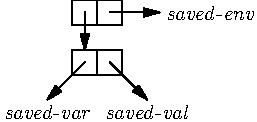
\includegraphics[scale=1.0]{alist-env.pdf}\end{SCentered}

\index{gzuan1lian2lie4biao3alist@关联列表 (a{-}list)|)idxdecorator{}{}}
\index{hzuan2jing4@环境!gzuan1lian2lie4biao3biao3shi4@关联列表表示|)idxdecorator{}{}}
这叫 \emph{a{-}list} 或\emph{关联列表} (\emph{association{-}list}) 表示法。\end{Subflow}\end{EoplExercise}

\begin{EoplExercise}\label{t:x28elem_x22ex2x2e6x22x29}\texMathInline{\textnormal{[}{\star}\textnormal{]}}\mbox{\hphantom{\Scribtexttt{x}}}发明三种以上的环境接口表示,给出实现。\end{EoplExercise}

\begin{EoplExercise}\label{t:x28elem_x22ex2x2e7x22x29}\texMathInline{\textnormal{[}{\star}\textnormal{]}}\mbox{\hphantom{\Scribtexttt{x}}}重写 中的 \Scribtexttt{apply{-}env},给出更详细的错误信息。\end{EoplExercise}

\begin{EoplExercise}\label{t:x28elem_x22ex2x2e8x22x29}\texMathInline{\textnormal{[}{\star}\textnormal{]}}\mbox{\hphantom{\Scribtexttt{x}}}\index{gzuan1lian2lie4biao3alist@关联列表 (a{-}list)|(idxdecorator{}{}}
\index{hzuan2jing4@环境!gzuan1lian2lie4biao3biao3shi4@关联列表表示|(idxdecorator{}{}}
给环境接口添加观测器 \Scribtexttt{empty{-}env{\hbox{\texttt{?}}}},用 a{-}list 表示法实现它。\end{EoplExercise}

\begin{EoplExercise}\label{t:x28elem_x22ex2x2e9x22x29}\texMathInline{\textnormal{[}{\star}\textnormal{]}}\mbox{\hphantom{\Scribtexttt{x}}}给环境接口添加观测器 \Scribtexttt{has{-}binding{\hbox{\texttt{?}}}},它取一环境 \texMathInline{env},一个变量 \texMathInline{s},判断
\texMathInline{s} 在 \texMathInline{env} 中是否有绑定值。用 a{-}list 表示法实现它。\end{EoplExercise}

\begin{EoplExercise}\label{t:x28elem_x22ex2x2e10x22x29}\texMathInline{\textnormal{[}{\star}\textnormal{]}}\mbox{\hphantom{\Scribtexttt{x}}}\index{extendenvasterisk@\textbf{\Scribtexttt{extend{-}env*}}|(idxdecorator{}{}}
给环境接口添加构造器 \Scribtexttt{extend{-}env*},用 a{-}list 表示法实现它。这个构造器取一变
量列表和一长度相等的值列表,以及一环境,其定义为:

\Iidentity{\begin{align*}& \Scribtexttt{(extend{-}env* (}\Iidentity{var_1}\Scribtexttt{ }\Iidentity{\dots}\Scribtexttt{ }\Iidentity{var_k}\Scribtexttt{) (}\Iidentity{val_1}\Scribtexttt{ }\Iidentity{\dots}\Scribtexttt{ }\Iidentity{var_k}\Scribtexttt{) }\Iidentity{\lceil f \rceil}\Scribtexttt{)} = \lceil g \rceil, \\
& \quad 其中,g(var) =
 \Iidentity{\begin{cases}val_i & 若 \ var = var_i \  对某个 \ i \ 成立,1 \leqslant i \leqslant k \\
f(var) & 否则\end{cases}}\end{align*}}
\index{gzuan1lian2lie4biao3alist@关联列表 (a{-}list)|)idxdecorator{}{}}
\index{hzuan2jing4@环境!gzuan1lian2lie4biao3biao3shi4@关联列表表示|)idxdecorator{}{}}\end{EoplExercise}

\begin{EoplExercise}\label{t:x28elem_x22ex2x2e11x22x29}\texMathInline{\textnormal{[}{\star}{\star}\textnormal{]}}\mbox{\hphantom{\Scribtexttt{x}}}前一题中的 \Scribtexttt{extend{-}env*} 实现比较拙劣的话,运行时间与 \texMathInline{k} 成正比。有一种表
示可使 \Scribtexttt{extend{-}env*} 的运行时间为常数:用空列表表示空环境,用下面的数据结构表
示非空环境:

\begin{SCentered}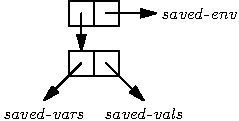
\includegraphics[scale=1.0]{rib-cage-one.pdf}\end{SCentered}

\begin{Subflow}那么一个环境看起来像是这样:

\begin{SCentered}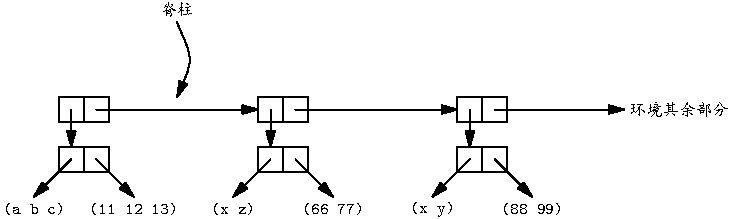
\includegraphics[scale=1.0]{rib-cage.pdf}\end{SCentered}

\index{hzuan2jing4@环境!lze1pai2biao3shi4@肋排表示|idxdecorator{}{}}
\index{tzui1li3gui1ze2@推理规则|idxdecorator{}{}}
这叫做\emph{肋排} (\emph{ribcage}) 表示法。环境由名为\emph{肋骨} (\emph{rib}) 的序对列表表示;
每根左肋是变量列表,右肋是对应的值列表。

用这种表示实现 \Scribtexttt{extend{-}env*} 和其他环境接口。
\index{szhu4ju4jie2gou4biao3shi4fa3@数据结构表示法!hzuan2jing4@环境|)idxdecorator{}{}}
\index{hzuan2jing4@环境!szhu4ju4jie2gou4biao3shi4@数据结构表示|)idxdecorator{}{}}
\index{extendenvasterisk@\textbf{\Scribtexttt{extend{-}env*}}|)idxdecorator{}{}}\end{Subflow}\end{EoplExercise}

\Ssubsubsection{过程表示法}{过程表示法}\label{t:x28part_x22s2x2e2x2e3x22x29}

\index{hzuan2jing4@环境!gzuo4cheng2biao3shi4@过程表示|(idxdecorator{}{}}
\index{gzuo4cheng2biao3shi4fa3@过程表示法!hzuan2jing4@环境|(idxdecorator{}{}}
环境接口有一条重要性质:它只有 \Scribtexttt{apply{-}env} 一个观测器。这样就能用取一变量,返
回绑定值的 Scheme 过程表示环境。

要这样表示,定义 \Scribtexttt{empty{-}env} 和 \Scribtexttt{extend{-}env} 的返回值为过程,调用二者的返
回值就如同调用上一节的 \Scribtexttt{apply{-}env} 一样。由此得出下面的实现。

\begin{EoplCodeInset}\begin{SCodeFlow}\begin{RktBlk}\begin{SingleColumn}\texMathInline{\mathit{Env} = \mathit{Var} \to \mathit{SchemeVal}}

\texMathInline{\mathit{Var} = \mathit{Sym}}

\mbox{\hphantom{\Scribtexttt{x}}}

\index{empty{-}env@\textbf{\Scribtexttt{empty{-}env}}|idxdecorator{}{}}

\textbf{\Scribtexttt{empty{-}env}} : \texMathInline{() \to \mathit{Env}}

\RktPn{(}\RktSym{define}\mbox{\hphantom{\Scribtexttt{x}}}\RktSym{empty{-}env}

\mbox{\hphantom{\Scribtexttt{xx}}}\RktPn{(}\RktSym{lambda}\mbox{\hphantom{\Scribtexttt{x}}}\RktPn{(}\RktPn{)}

\mbox{\hphantom{\Scribtexttt{xxxx}}}\RktPn{(}\RktSym{lambda}\mbox{\hphantom{\Scribtexttt{x}}}\RktPn{(}\RktSym{search{-}var}\RktPn{)}

\mbox{\hphantom{\Scribtexttt{xxxxxx}}}\RktPn{(}\RktSym{report{-}no{-}binding{-}found}\mbox{\hphantom{\Scribtexttt{x}}}\RktSym{search{-}var}\RktPn{)}\RktPn{)}\RktPn{)}\RktPn{)}

\mbox{\hphantom{\Scribtexttt{x}}}

\index{extendenv@\textbf{\Scribtexttt{extend{-}env}}|idxdecorator{}{}}

\textbf{\Scribtexttt{extend{-}env}} : \texMathInline{\mathit{Var} \times \mathit{SchemeVal} \times \mathit{Env} \to \mathit{Env}}

\RktPn{(}\RktSym{define}\mbox{\hphantom{\Scribtexttt{x}}}\RktSym{extend{-}env}

\mbox{\hphantom{\Scribtexttt{xx}}}\RktPn{(}\RktSym{lambda}\mbox{\hphantom{\Scribtexttt{x}}}\RktPn{(}\RktSym{saved{-}var}\mbox{\hphantom{\Scribtexttt{x}}}\RktSym{saved{-}val}\mbox{\hphantom{\Scribtexttt{x}}}\RktSym{saved{-}env}\RktPn{)}

\mbox{\hphantom{\Scribtexttt{xxxx}}}\RktPn{(}\RktSym{lambda}\mbox{\hphantom{\Scribtexttt{x}}}\RktPn{(}\RktSym{search{-}var}\RktPn{)}

\mbox{\hphantom{\Scribtexttt{xxxxxx}}}\RktPn{(}\RktSym{if}\mbox{\hphantom{\Scribtexttt{x}}}\RktPn{(}\RktSym{eqv{\hbox{\texttt{?}}}}\mbox{\hphantom{\Scribtexttt{x}}}\RktSym{search{-}var}\mbox{\hphantom{\Scribtexttt{x}}}\RktSym{saved{-}var}\RktPn{)}

\mbox{\hphantom{\Scribtexttt{xxxxxxxx}}}\RktSym{saved{-}val}

\mbox{\hphantom{\Scribtexttt{xxxxxxxx}}}\RktPn{(}\RktSym{apply{-}env}\mbox{\hphantom{\Scribtexttt{x}}}\RktSym{saved{-}env}\mbox{\hphantom{\Scribtexttt{x}}}\RktSym{search{-}var}\RktPn{)}\RktPn{)}\RktPn{)}\RktPn{)}\RktPn{)}

\mbox{\hphantom{\Scribtexttt{x}}}

\index{applyenv@\textbf{\Scribtexttt{apply{-}env}}|idxdecorator{}{}}

\textbf{\Scribtexttt{apply{-}env}} : \texMathInline{\mathit{Env} \times \mathit{Var} \to \mathit{SchemeVal}}

\RktPn{(}\RktSym{define}\mbox{\hphantom{\Scribtexttt{x}}}\RktSym{apply{-}env}

\mbox{\hphantom{\Scribtexttt{xx}}}\RktPn{(}\RktSym{lambda}\mbox{\hphantom{\Scribtexttt{x}}}\RktPn{(}\RktSym{env}\mbox{\hphantom{\Scribtexttt{x}}}\RktSym{search{-}var}\RktPn{)}

\mbox{\hphantom{\Scribtexttt{xxxx}}}\RktPn{(}\RktSym{env}\mbox{\hphantom{\Scribtexttt{x}}}\RktSym{search{-}var}\RktPn{)}\RktPn{)}\RktPn{)}\end{SingleColumn}\end{RktBlk}\end{SCodeFlow}\end{EoplCodeInset}

\Scribtexttt{empty{-}env} 创建的空环境收到任何变量都会报错,表明给定的变量不在其中。过程
\Scribtexttt{extend{-}env} 返回的过程代表扩展而得的环境。这个过程收到变量 \Scribtexttt{search{-}var}
后,判断该变量是否与环境中绑定的相同。如果相同,就返回保存的值;否则,就在保存的
环境中查找它。

这种表示法中,数据由 \Scribtexttt{apply{-}env} \emph{执行的动作}表示,我们称之
为\emph{过程表示法} (\emph{procedural representation})。

数据类型只有一个观测器的情形并非想象中那般少见。比如,当数据是一组函数,就能用调
用时执行的动作\index{dziao4yong4shi2zhi2xing2dedong4zuo4@调用时执行的动作|idxdecorator{}{}}表示。这种情况下,可以按照下
列步骤提炼出接口和过程表示法:

\begin{enumerate}\atItemizeStart

\item 找出客户代码中求取指定类型值的 lambda 表达式。为每个这样的 lambda 表达式
写一个构造器过程。构造器过程的参数用作 lambda 表达式中的自由变量。在客户代码中,
用构造器调用替换对应的 lambda 表达式。

\item 像定义 \Scribtexttt{apply{-}env} 那样定义一个 \Scribtexttt{apply{-}} 过程。找出客户代码中所有使
用指定类型值的地方,包括构造器过程的主体。所有使用指定类型值的地方都改用
\Scribtexttt{apply{-}} 过程。\end{enumerate}

\index{applygzuo4cheng2@\Scribtexttt{apply{-}} 过程|idxdecorator{}{}}
一旦完成这些步骤,接口就包含所有的构造器过程和 \Scribtexttt{apply{-}} 过程,客户代码则与表
示无关:它不再依赖表示,我们将能随意换用另一套接口实现,正如 \SecRefLocal{t:x28part_x22s2x2e2x2e2x22x29}{2.2.2}{数据结构表示法}所述。

如果用于实现的语言不支持高阶过程,那就得再做一些步骤,用数据结构表示法和解释器秘
方实现所需接口,就像上一节那样。这一操作叫做\emph{消函} (\emph{defunctionalization})。
\index{xziao1han2@消函|idxdecorator{}{}}
环境的数据结构表示中,各种变体都是消函的简单例子。过程表示法和消函表示法的关系将
是本书反复出现的主题。
\index{hzuan2jing4@环境!gzuo4cheng2biao3shi4@过程表示|)idxdecorator{}{}}
\index{gzuo4cheng2biao3shi4fa3@过程表示法!hzuan2jing4@环境|)idxdecorator{}{}}

\begin{EoplExercise}\label{t:x28elem_x22ex2x2e12x22x29}\texMathInline{\textnormal{[}{\star}\textnormal{]}}\mbox{\hphantom{\Scribtexttt{x}}}\index{hzuan2jing4@环境!gzuo4cheng2biao3shi4@过程表示|(idxdecorator{}{}}
\index{gzuo4cheng2biao3shi4fa3@过程表示法!hzuan2jing4@环境|(idxdecorator{}{}}
\index{gzuo4cheng2biao3shi4fa3@过程表示法!zzhan4@栈|idxdecorator{}{}}
\index{zzhan4@栈|idxdecorator{}{}}
用过程表示法实现ex2.4 中的栈数据类型。\end{EoplExercise}

\begin{EoplExercise}\label{t:x28elem_x22ex2x2e13x22x29}\texMathInline{\textnormal{[}{\star}{\star}\textnormal{]}}\mbox{\hphantom{\Scribtexttt{x}}}扩展过程表示法,用两个过程组成的列表表示环境,实现 \Scribtexttt{empty{-}env{\hbox{\texttt{?}}}}。一个过程像前
面那样,返回变量的绑定值;一个返回环境是否为空。\end{EoplExercise}

\begin{EoplExercise}\label{t:x28elem_x22ex2x2e14x22x29}\texMathInline{\textnormal{[}{\star}{\star}\textnormal{]}}\mbox{\hphantom{\Scribtexttt{x}}}扩展前一题中的表示法,加入第三个过程,用它来 \Scribtexttt{has{-}binding{\hbox{\texttt{?}}}} (见
ex2.9)。
\index{hzuan2jing4@环境!gzuo4cheng2biao3shi4@过程表示|)idxdecorator{}{}}
\index{gzuo4cheng2biao3shi4fa3@过程表示法!hzuan2jing4@环境|)idxdecorator{}{}}\end{EoplExercise}

\Ssubsection{递推数据类型的接口}{递推数据类型的接口}\label{t:x28part_x22s2x2e3x22x29}

\index{Lambdabziao3da2shi4LcExp@Lambda 表达式 (LcExp)|(idxdecorator{}{}}
\ChapRefLocal{t:x28part_x22isdx22x29}{1}{归纳式数据集}大部分都在处理递推数据类型。例如, 给出了
lambda 演算表达式的语法:

\Iidentity{\begin{align*}\mathit{Lc\mbox{-}Exp}
&::= \mathit{Identifier} \\
&::= \normalfont{\Scribtexttt{(lambda (}\Iidentity{\mathit{Identifier}}\Scribtexttt{) }\Iidentity{\mathit{Lc\mbox{-}Exp}}\Scribtexttt{)}} \\
&::= \normalfont{\Scribtexttt{(}\Iidentity{\mathit{Lc\mbox{-}Exp}}\Scribtexttt{ }\Iidentity{\mathit{Lc\mbox{-}Exp}}\Scribtexttt{)}}\end{align*}}

我们还写出了过程 \Scribtexttt{occurs{-}free{\hbox{\texttt{?}}}}。像当时提到的,\SecRefLocal{t:x28part_x22s1x2e2x2e4x22x29}{1.2.4}{\Scribtexttt{occurs{-}free{\hbox{\texttt{?}}}}}中
\Scribtexttt{occurs{-}free{\hbox{\texttt{?}}}} 的定义不大容易读懂。比如,很难搞明白 \Scribtexttt{(car (cadr exp))} 指
代 \Scribtexttt{lambda} 表达式中的变量声明,或者 \Scribtexttt{(caddr exp)} 指代表达式的主体。

\index{wzei4ci2@谓词|(idxdecorator{}{}}
要改善这种情况,可以给 lambda 演算表达式添加一套接口。我们的接口有几个构造器,以
及两种观测器:谓词和提取器。

构造器有:

\begin{SInsetFlow}\begin{SVerbatim}\begin{SingleColumn}\textbf{\Scribtexttt{var{-}exp}}\Scribtexttt{{\hbox{\texttt{:}}} }\texMathInline{\mathit{Var} \to \mathit{Lc\mbox{-}Exp}}\Scribtexttt{}

\Scribtexttt{}\textbf{\Scribtexttt{lambda{-}exp}}\Scribtexttt{{\hbox{\texttt{:}}} }\texMathInline{\mathit{Var} \times \mathit{Lc\mbox{-}Exp} \to \mathit{Lc\mbox{-}Exp}}\Scribtexttt{}

\Scribtexttt{}\textbf{\Scribtexttt{app{-}exp}}\Scribtexttt{{\hbox{\texttt{:}}} }\texMathInline{\mathit{Lc\mbox{-}Exp} \times \mathit{Lc\mbox{-}Exp} \to \mathit{Lc\mbox{-}Exp}}\end{SingleColumn}\end{SVerbatim}\end{SInsetFlow}

谓词有:

\begin{SInsetFlow}\begin{SVerbatim}\begin{SingleColumn}\textbf{\Scribtexttt{var{-}exp{\hbox{\texttt{?}}}}}\Scribtexttt{{\hbox{\texttt{:}}} }\texMathInline{\mathit{Lc\mbox{-}Exp} \to \mathit{Bool}}\Scribtexttt{}

\Scribtexttt{}\textbf{\Scribtexttt{lambda{-}exp{\hbox{\texttt{?}}}}}\Scribtexttt{{\hbox{\texttt{:}}} }\texMathInline{\mathit{Lc\mbox{-}Exp} \to \mathit{Bool}}\Scribtexttt{}

\Scribtexttt{}\textbf{\Scribtexttt{app{-}exp{\hbox{\texttt{?}}}}}\Scribtexttt{{\hbox{\texttt{:}}} }\texMathInline{\mathit{Lc\mbox{-}Exp} \to \mathit{Bool}}\end{SingleColumn}\end{SVerbatim}\end{SInsetFlow}

\index{tzi2qu3qi4@提取器|(idxdecorator{}{}}
提取器有:

\begin{SInsetFlow}\begin{SVerbatim}\begin{SingleColumn}\textbf{\Scribtexttt{var{-}exp{-}{\Stttextmore}var}}\Scribtexttt{{\hbox{\texttt{:}}} }\texMathInline{\mathit{Lc\mbox{-}Exp} \to \mathit{Var}}\Scribtexttt{}

\Scribtexttt{}\textbf{\Scribtexttt{lambda{-}exp{-}{\Stttextmore}bound{-}var}}\Scribtexttt{{\hbox{\texttt{:}}} }\texMathInline{\mathit{Lc\mbox{-}Exp} \to \mathit{Var}}\Scribtexttt{}

\Scribtexttt{}\textbf{\Scribtexttt{lambda{-}exp{-}{\Stttextmore}body}}\Scribtexttt{{\hbox{\texttt{:}}} }\texMathInline{\mathit{Lc\mbox{-}Exp} \to \mathit{Lc\mbox{-}Exp}}\Scribtexttt{}

\Scribtexttt{}\textbf{\Scribtexttt{app{-}exp{-}{\Stttextmore}rator}}\Scribtexttt{{\hbox{\texttt{:}}} }\texMathInline{\mathit{Lc\mbox{-}Exp} \to \mathit{Lc\mbox{-}Exp}}\Scribtexttt{}

\Scribtexttt{}\textbf{\Scribtexttt{app{-}exp{-}{\Stttextmore}rand}}\Scribtexttt{{\hbox{\texttt{:}}} }\texMathInline{\mathit{Lc\mbox{-}Exp} \to \mathit{Lc\mbox{-}Exp}}\end{SingleColumn}\end{SVerbatim}\end{SInsetFlow}

每个提取器对应 lambda 演算表达式中的一部分。现在可以写出一版只依赖接口的
\Scribtexttt{occurs{-}free{\hbox{\texttt{?}}}}。

\begin{EoplCodeInset}\index{occursfree@\textbf{\Scribtexttt{occurs{-}free{\hbox{\texttt{?}}}}}|(idxdecorator{}{}}


\begin{SCodeFlow}\begin{RktBlk}\begin{SingleColumn}\label{t:x28elem_x22occursx2dfreex3fx22x29}\textbf{\Scribtexttt{occurs{-}free{\hbox{\texttt{?}}}}} : \texMathInline{\mathit{Sym} \times \mathit{LcExp} \to \mathit{Bool}}

\RktPn{(}\RktSym{define}\mbox{\hphantom{\Scribtexttt{x}}}\RktSym{occurs{-}free{\hbox{\texttt{?}}}}

\mbox{\hphantom{\Scribtexttt{xx}}}\RktPn{(}\RktSym{lambda}\mbox{\hphantom{\Scribtexttt{x}}}\RktPn{(}\RktSym{search{-}var}\mbox{\hphantom{\Scribtexttt{x}}}\RktSym{exp}\RktPn{)}

\mbox{\hphantom{\Scribtexttt{xxxx}}}\RktPn{(}\RktSym{cond}

\mbox{\hphantom{\Scribtexttt{xxxxxx}}}\RktPn{(}\RktPn{(}\RktSym{var{-}exp{\hbox{\texttt{?}}}}\mbox{\hphantom{\Scribtexttt{x}}}\RktSym{exp}\RktPn{)}\mbox{\hphantom{\Scribtexttt{x}}}\RktPn{(}\RktSym{eqv{\hbox{\texttt{?}}}}\mbox{\hphantom{\Scribtexttt{x}}}\RktSym{search{-}var}\mbox{\hphantom{\Scribtexttt{x}}}\RktPn{(}\RktSym{var{-}exp{-}{\Stttextmore}var}\mbox{\hphantom{\Scribtexttt{x}}}\RktSym{exp}\RktPn{)}\RktPn{)}\RktPn{)}

\mbox{\hphantom{\Scribtexttt{xxxxxx}}}\RktPn{(}\RktPn{(}\RktSym{lambda{-}exp{\hbox{\texttt{?}}}}\mbox{\hphantom{\Scribtexttt{x}}}\RktSym{exp}\RktPn{)}

\mbox{\hphantom{\Scribtexttt{xxxxxxxx}}}\RktPn{(}\RktSym{and}

\mbox{\hphantom{\Scribtexttt{xxxxxxxxxx}}}\RktPn{(}\RktSym{not}\mbox{\hphantom{\Scribtexttt{x}}}\RktPn{(}\RktSym{eqv{\hbox{\texttt{?}}}}\mbox{\hphantom{\Scribtexttt{x}}}\RktSym{search{-}var}\mbox{\hphantom{\Scribtexttt{x}}}\RktPn{(}\RktSym{lambda{-}exp{-}{\Stttextmore}bound{-}var}\mbox{\hphantom{\Scribtexttt{x}}}\RktSym{exp}\RktPn{)}\RktPn{)}\RktPn{)}

\mbox{\hphantom{\Scribtexttt{xxxxxxxxxx}}}\RktPn{(}\RktSym{occurs{-}free{\hbox{\texttt{?}}}}\mbox{\hphantom{\Scribtexttt{x}}}\RktSym{search{-}var}\mbox{\hphantom{\Scribtexttt{x}}}\RktPn{(}\RktSym{lambda{-}exp{-}{\Stttextmore}body}\mbox{\hphantom{\Scribtexttt{x}}}\RktSym{exp}\RktPn{)}\RktPn{)}\RktPn{)}\RktPn{)}

\mbox{\hphantom{\Scribtexttt{xxxxxx}}}\RktPn{(}\RktSym{else}

\mbox{\hphantom{\Scribtexttt{xxxxxxxx}}}\RktPn{(}\RktSym{or}

\mbox{\hphantom{\Scribtexttt{xxxxxxxxxx}}}\RktPn{(}\RktSym{occurs{-}free{\hbox{\texttt{?}}}}\mbox{\hphantom{\Scribtexttt{x}}}\RktSym{search{-}var}\mbox{\hphantom{\Scribtexttt{x}}}\RktPn{(}\RktSym{app{-}exp{-}{\Stttextmore}rator}\mbox{\hphantom{\Scribtexttt{x}}}\RktSym{exp}\RktPn{)}\RktPn{)}

\mbox{\hphantom{\Scribtexttt{xxxxxxxxxx}}}\RktPn{(}\RktSym{occurs{-}free{\hbox{\texttt{?}}}}\mbox{\hphantom{\Scribtexttt{x}}}\RktSym{search{-}var}\mbox{\hphantom{\Scribtexttt{x}}}\RktPn{(}\RktSym{app{-}exp{-}{\Stttextmore}rand}\mbox{\hphantom{\Scribtexttt{x}}}\RktSym{exp}\RktPn{)}\RktPn{)}\RktPn{)}\RktPn{)}\RktPn{)}\RktPn{)}\RktPn{)}\end{SingleColumn}\end{RktBlk}\end{SCodeFlow}

\noindent \index{occursfree@\textbf{\Scribtexttt{occurs{-}free{\hbox{\texttt{?}}}}}|)idxdecorator{}{}}\end{EoplCodeInset}

只要使用上述构造器,怎样表示 lambda 演算表达式都可以。
\index{Lambdabziao3da2shi4LcExp@Lambda 表达式 (LcExp)|)idxdecorator{}{}}

\index{gzou4zao4qi4@构造器|idxdecorator{}{}}
我们可以写出设计递推数据类型接口的一般步骤:

\begin{Tip}\begin{SCentered}\textbf{设计递推数据类型的接口}\end{SCentered}

\begin{TipContent}\begin{enumerate}\atItemizeStart

\item 为数据类型的每种变体加入一个构造器。

\item 为数据类型的每种变体加入一个谓词。

\item 为传给数据类型构造器的每段数据加入一个提取器。
\index{tzi2qu3qi4@提取器|)idxdecorator{}{}}
\index{wzei4ci2@谓词|)idxdecorator{}{}}\end{enumerate}\end{TipContent}\end{Tip}

\begin{EoplExercise}\label{t:x28elem_x22ex2x2e15x22x29}\texMathInline{\textnormal{[}{\star}\textnormal{]}}\mbox{\hphantom{\Scribtexttt{x}}}\index{Lambdabziao3da2shi4LcExp@Lambda 表达式 (LcExp)|(idxdecorator{}{}}
上述语法指定了 lambda 演算表达式的表示方式,实现其接口。\end{EoplExercise}

\begin{EoplExercise}\label{t:x28elem_x22ex2x2e16x22x29}\texMathInline{\textnormal{[}{\star}\textnormal{]}}\mbox{\hphantom{\Scribtexttt{x}}}修改实现,换用另一种表示,去掉 \Scribtexttt{lambda} 表达式绑定变量周围的括号。\end{EoplExercise}

\begin{EoplExercise}\label{t:x28elem_x22ex2x2e17x22x29}\texMathInline{\textnormal{[}{\star}\textnormal{]}}\mbox{\hphantom{\Scribtexttt{x}}}再发明至少两种方式来表示数据类型 lambda 演算表达式,实现它们。
\index{Lambdabziao3da2shi4LcExp@Lambda 表达式 (LcExp)|)idxdecorator{}{}}\end{EoplExercise}

\begin{EoplExercise}\label{t:x28elem_x22ex2x2e18x22x29}\texMathInline{\textnormal{[}{\star}\textnormal{]}}\mbox{\hphantom{\Scribtexttt{x}}}\index{szhuang1xiang4xu4lie4@双向序列|(idxdecorator{}{}}
\index{szhuang1xiang4xu4lie4@双向序列|(idxdecorator{}{}}
我们常用列表表示值的序列。在这种表示法中,很容易从序列中的一个元素移动到下一个,
但是不借助上下文参数,很难从一个元素移动到上一个。实现非空双向整数序列,语法为:

\Iidentity{\[\mathit{NodeInSequence} ::= \Scribtexttt{(}\Iidentity{\mathit{Int}}\Scribtexttt{
}\Iidentity{\mathit{Listof\Scribtexttt{(}\Iidentity{\mathit{Int}}\Scribtexttt{)}}}\Scribtexttt{ }\Iidentity{\mathit{Listof\Scribtexttt{(}\Iidentity{\mathit{Int}}\Scribtexttt{)}}}\Scribtexttt{)}\]}

第一个整数列表是当前元素之前的序列,反向排列。第二个列表是当前元素之后的序列。例
如,\Scribtexttt{(6 (5 4 3 2 1) (7 8 9))} 表示列表 \Scribtexttt{(1 2 3 4 5 6 7 8 9)},当前元素为6。

用这种表示实现过程 \Scribtexttt{number{-}{\Stttextmore}sequence},它取一数字,生成只包含该数字的序列。接
着实现 \Scribtexttt{current{-}element}、\Scribtexttt{move{-}to{-}left}、\Scribtexttt{move{-}to{-}right}、
\Scribtexttt{insert{-}to{-}left}、\Scribtexttt{insert{-}to{-}right}、\Scribtexttt{at{-}left{-}end{\hbox{\texttt{?}}}} 和
\Scribtexttt{at{-}right{-}end{\hbox{\texttt{?}}}}。

例如:

\begin{EoplCodeInset}\begin{SCodeFlow}\begin{RktBlk}\begin{SingleColumn}\Scribtexttt{{\Stttextmore} }\RktPn{(}\RktSym{number{-}{\Stttextmore}sequence}\mbox{\hphantom{\Scribtexttt{x}}}\RktVal{7}\RktPn{)}

\RktRes{{\textquotesingle}(7\Scribtexttt{ }()\Scribtexttt{ }())}

\Scribtexttt{{\Stttextmore} }\RktPn{(}\RktSym{current{-}element}\mbox{\hphantom{\Scribtexttt{x}}}\RktVal{{\textquotesingle}}\RktVal{(}\RktVal{6}\mbox{\hphantom{\Scribtexttt{x}}}\RktVal{(}\RktVal{5}\mbox{\hphantom{\Scribtexttt{x}}}\RktVal{4}\mbox{\hphantom{\Scribtexttt{x}}}\RktVal{3}\mbox{\hphantom{\Scribtexttt{x}}}\RktVal{2}\mbox{\hphantom{\Scribtexttt{x}}}\RktVal{1}\RktVal{)}\mbox{\hphantom{\Scribtexttt{x}}}\RktVal{(}\RktVal{7}\mbox{\hphantom{\Scribtexttt{x}}}\RktVal{8}\mbox{\hphantom{\Scribtexttt{x}}}\RktVal{9}\RktVal{)}\RktVal{)}\RktPn{)}

\RktRes{6}

\Scribtexttt{{\Stttextmore} }\RktPn{(}\RktSym{move{-}to{-}left}\mbox{\hphantom{\Scribtexttt{x}}}\RktVal{{\textquotesingle}}\RktVal{(}\RktVal{6}\mbox{\hphantom{\Scribtexttt{x}}}\RktVal{(}\RktVal{5}\mbox{\hphantom{\Scribtexttt{x}}}\RktVal{4}\mbox{\hphantom{\Scribtexttt{x}}}\RktVal{3}\mbox{\hphantom{\Scribtexttt{x}}}\RktVal{2}\mbox{\hphantom{\Scribtexttt{x}}}\RktVal{1}\RktVal{)}\mbox{\hphantom{\Scribtexttt{x}}}\RktVal{(}\RktVal{7}\mbox{\hphantom{\Scribtexttt{x}}}\RktVal{8}\mbox{\hphantom{\Scribtexttt{x}}}\RktVal{9}\RktVal{)}\RktVal{)}\RktPn{)}

\RktRes{{\textquotesingle}(5\Scribtexttt{ }(4\Scribtexttt{ }3\Scribtexttt{ }2\Scribtexttt{ }1)\Scribtexttt{ }(6\Scribtexttt{ }7\Scribtexttt{ }8\Scribtexttt{ }9))}

\Scribtexttt{{\Stttextmore} }\RktPn{(}\RktSym{move{-}to{-}right}\mbox{\hphantom{\Scribtexttt{x}}}\RktVal{{\textquotesingle}}\RktVal{(}\RktVal{6}\mbox{\hphantom{\Scribtexttt{x}}}\RktVal{(}\RktVal{5}\mbox{\hphantom{\Scribtexttt{x}}}\RktVal{4}\mbox{\hphantom{\Scribtexttt{x}}}\RktVal{3}\mbox{\hphantom{\Scribtexttt{x}}}\RktVal{2}\mbox{\hphantom{\Scribtexttt{x}}}\RktVal{1}\RktVal{)}\mbox{\hphantom{\Scribtexttt{x}}}\RktVal{(}\RktVal{7}\mbox{\hphantom{\Scribtexttt{x}}}\RktVal{8}\mbox{\hphantom{\Scribtexttt{x}}}\RktVal{9}\RktVal{)}\RktVal{)}\RktPn{)}

\RktRes{{\textquotesingle}(7\Scribtexttt{ }(6\Scribtexttt{ }5\Scribtexttt{ }4\Scribtexttt{ }3\Scribtexttt{ }2\Scribtexttt{ }1)\Scribtexttt{ }(8\Scribtexttt{ }9))}

\Scribtexttt{{\Stttextmore} }\RktPn{(}\RktSym{insert{-}to{-}left}\mbox{\hphantom{\Scribtexttt{x}}}\RktVal{13}\mbox{\hphantom{\Scribtexttt{x}}}\RktVal{{\textquotesingle}}\RktVal{(}\RktVal{6}\mbox{\hphantom{\Scribtexttt{x}}}\RktVal{(}\RktVal{5}\mbox{\hphantom{\Scribtexttt{x}}}\RktVal{4}\mbox{\hphantom{\Scribtexttt{x}}}\RktVal{3}\mbox{\hphantom{\Scribtexttt{x}}}\RktVal{2}\mbox{\hphantom{\Scribtexttt{x}}}\RktVal{1}\RktVal{)}\mbox{\hphantom{\Scribtexttt{x}}}\RktVal{(}\RktVal{7}\mbox{\hphantom{\Scribtexttt{x}}}\RktVal{8}\mbox{\hphantom{\Scribtexttt{x}}}\RktVal{9}\RktVal{)}\RktVal{)}\RktPn{)}

\RktRes{{\textquotesingle}(6\Scribtexttt{ }(13\Scribtexttt{ }5\Scribtexttt{ }4\Scribtexttt{ }3\Scribtexttt{ }2\Scribtexttt{ }1)\Scribtexttt{ }(7\Scribtexttt{ }8\Scribtexttt{ }9))}

\Scribtexttt{{\Stttextmore} }\RktPn{(}\RktSym{insert{-}to{-}right}\mbox{\hphantom{\Scribtexttt{x}}}\RktVal{13}\mbox{\hphantom{\Scribtexttt{x}}}\RktVal{{\textquotesingle}}\RktVal{(}\RktVal{6}\mbox{\hphantom{\Scribtexttt{x}}}\RktVal{(}\RktVal{5}\mbox{\hphantom{\Scribtexttt{x}}}\RktVal{4}\mbox{\hphantom{\Scribtexttt{x}}}\RktVal{3}\mbox{\hphantom{\Scribtexttt{x}}}\RktVal{2}\mbox{\hphantom{\Scribtexttt{x}}}\RktVal{1}\RktVal{)}\mbox{\hphantom{\Scribtexttt{x}}}\RktVal{(}\RktVal{7}\mbox{\hphantom{\Scribtexttt{x}}}\RktVal{8}\mbox{\hphantom{\Scribtexttt{x}}}\RktVal{9}\RktVal{)}\RktVal{)}\RktPn{)}

\RktRes{{\textquotesingle}(6\Scribtexttt{ }(5\Scribtexttt{ }4\Scribtexttt{ }3\Scribtexttt{ }2\Scribtexttt{ }1)\Scribtexttt{ }(13\Scribtexttt{ }7\Scribtexttt{ }8\Scribtexttt{ }9))}\end{SingleColumn}\end{RktBlk}\end{SCodeFlow}\end{EoplCodeInset}

如果参数在序列最右端,过程\Scribtexttt{move{-}to{-}right}应失败。如果参数在序列最左端,过程
\Scribtexttt{move{-}to{-}left}应失败。
\index{szhuang1xiang4xu4lie4@双向序列|)idxdecorator{}{}}
\index{szhuang1xiang4xu4lie4@双向序列|)idxdecorator{}{}}\end{EoplExercise}

\begin{EoplExercise}\label{t:x28elem_x22ex2x2e19x22x29}\texMathInline{\textnormal{[}{\star}\textnormal{]}}\mbox{\hphantom{\Scribtexttt{x}}}\index{ezr4cha1shu4@二叉树 (\texMathInline{\mathit{Bintree}})|idxdecorator{}{}}
空二叉树和用整数标记内部节点的二叉树可以用语法表示为:

\Iidentity{\[\mathit{BinTree} ::= \Scribtexttt{()} \mid \Scribtexttt{(}\Iidentity{\mathit{Int}}\Scribtexttt{ }\Iidentity{\mathit{BinTree}}\Scribtexttt{
}\Iidentity{\mathit{BinTree}}\Scribtexttt{)}\]}

用这种表示实现过程 \Scribtexttt{number{-}{\Stttextmore}bintree},它取一个整数,产生一棵新的二叉树,树的
唯一节点包含该数字。接着实现 \Scribtexttt{current{-}element}、\Scribtexttt{move{-}to{-}left{-}son}、
\Scribtexttt{move{-}to{-}right{-}son}、\Scribtexttt{at{-}leaf{\hbox{\texttt{?}}}}、\Scribtexttt{insert{-}to{-}left} 和
\Scribtexttt{insert{-}to{-}right}。例如:

\begin{EoplCodeInset}\begin{SCodeFlow}\begin{RktBlk}\begin{SingleColumn}\Scribtexttt{{\Stttextmore} }\RktPn{(}\RktSym{number{-}{\Stttextmore}bintree}\mbox{\hphantom{\Scribtexttt{x}}}\RktVal{13}\RktPn{)}

\RktRes{{\textquotesingle}(13\Scribtexttt{ }()\Scribtexttt{ }())}

\begin{RktBlk}\begin{SingleColumn}\Scribtexttt{{\Stttextmore} }\RktPn{(}\RktSym{define}\mbox{\hphantom{\Scribtexttt{x}}}\RktSym{t1}\mbox{\hphantom{\Scribtexttt{x}}}\RktPn{(}\RktSym{insert{-}to{-}right}\mbox{\hphantom{\Scribtexttt{x}}}\RktVal{14}

\mbox{\hphantom{\Scribtexttt{xx}}}\mbox{\hphantom{\Scribtexttt{xxxxxxxxxxxxx}}}\RktPn{(}\RktSym{insert{-}to{-}left}\mbox{\hphantom{\Scribtexttt{x}}}\RktVal{12}

\mbox{\hphantom{\Scribtexttt{xx}}}\mbox{\hphantom{\Scribtexttt{xxxxxxxxxxxxxxx}}}\RktPn{(}\RktSym{number{-}{\Stttextmore}bintree}\mbox{\hphantom{\Scribtexttt{x}}}\RktVal{13}\RktPn{)}\RktPn{)}\RktPn{)}\RktPn{)}\end{SingleColumn}\end{RktBlk}

\Scribtexttt{{\Stttextmore} }\RktSym{t1}

\RktRes{{\textquotesingle}(13\Scribtexttt{ }(12\Scribtexttt{ }()\Scribtexttt{ }())\Scribtexttt{ }(14\Scribtexttt{ }()\Scribtexttt{ }()))}

\Scribtexttt{{\Stttextmore} }\RktPn{(}\RktSym{move{-}to{-}left{-}son}\mbox{\hphantom{\Scribtexttt{x}}}\RktSym{t1}\RktPn{)}

\RktRes{{\textquotesingle}(12\Scribtexttt{ }()\Scribtexttt{ }())}

\Scribtexttt{{\Stttextmore} }\RktPn{(}\RktSym{current{-}element}\mbox{\hphantom{\Scribtexttt{x}}}\RktPn{(}\RktSym{move{-}to{-}left{-}son}\mbox{\hphantom{\Scribtexttt{x}}}\RktSym{t1}\RktPn{)}\RktPn{)}

\RktRes{12}

\Scribtexttt{{\Stttextmore} }\RktPn{(}\RktSym{at{-}leaf{\hbox{\texttt{?}}}}\mbox{\hphantom{\Scribtexttt{x}}}\RktPn{(}\RktSym{move{-}to{-}right{-}son}\mbox{\hphantom{\Scribtexttt{x}}}\RktPn{(}\RktSym{move{-}to{-}left{-}son}\mbox{\hphantom{\Scribtexttt{x}}}\RktSym{t1}\RktPn{)}\RktPn{)}\RktPn{)}

\RktRes{\#t}

\Scribtexttt{{\Stttextmore} }\RktPn{(}\RktSym{insert{-}to{-}left}\mbox{\hphantom{\Scribtexttt{x}}}\RktVal{15}\mbox{\hphantom{\Scribtexttt{x}}}\RktSym{t1}\RktPn{)}

\RktRes{{\textquotesingle}(13\Scribtexttt{ }(15\Scribtexttt{ }(12\Scribtexttt{ }()\Scribtexttt{ }())\Scribtexttt{ }())\Scribtexttt{ }(14\Scribtexttt{ }()\Scribtexttt{ }()))}\end{SingleColumn}\end{RktBlk}\end{SCodeFlow}\end{EoplCodeInset}\end{EoplExercise}

\begin{EoplExercise}\label{t:x28elem_x22ex2x2e20x22x29}\texMathInline{\textnormal{[}{\star}{\star}{\star}\textnormal{]}}\mbox{\hphantom{\Scribtexttt{x}}}按照ex2.19 中的二叉树表示,很容易从父节点移到某个子节点,但是不借
助上下文参数,无法从子节点移动到父节点。扩展ex2.18 中的列表表示法,
用以表示二叉树中的节点。提示:想想怎样用逆序列表表示二叉树在当前节点以上的部分,
就像ex2.18 那样。

用这种表示实现ex2.19 中的过程。接着实现 \Scribtexttt{move{-}up} 和
\Scribtexttt{at{-}root{\hbox{\texttt{?}}}}。\end{EoplExercise}

\Ssubsection{定义递推数据类型的工具}{定义递推数据类型的工具}\label{t:x28part_x22s2x2e4x22x29}

\index{dzi4tui1shu4ju4lei4xing2@递推数据类型!czhu4li3cheng2xu4@处理程序|(idxdecorator{}{}}
对复杂的数据类型,按照上述步骤设计接口很快就会使人厌倦。本节介绍用 Scheme 自动设
计和实现接口的工具。这个工具产生的接口与前一节的虽不完全相同,却很类似。

\index{definedatatypexzing2shi4@\Scribtexttt{define{-}datatype} 形式|(idxdecorator{}{}}
\index{Lambdabziao3da2shi4LcExp@Lambda 表达式 (LcExp)!Schemeszhi2xian4@Scheme 实现|(idxdecorator{}{}}
仍考虑前一节讨论的数据类型 lambda 演算表达式。lambda 演算表达式的接口可以这样写:

\begin{EoplCodeInset}\begin{SCodeFlow}\begin{RktBlk}\begin{SingleColumn}\RktPn{(}\label{t:x28elem_x22lcx2dexpx22x29}\RktSym{define{-}datatype}\mbox{\hphantom{\Scribtexttt{x}}}\RktSym{lc{-}exp}\mbox{\hphantom{\Scribtexttt{x}}}\RktSym{lc{-}exp{\hbox{\texttt{?}}}}

\mbox{\hphantom{\Scribtexttt{xx}}}\RktPn{(}\RktSym{var{-}exp}

\mbox{\hphantom{\Scribtexttt{xxx}}}\RktPn{(}\RktSym{var}\mbox{\hphantom{\Scribtexttt{x}}}\RktSym{identifier{\hbox{\texttt{?}}}}\RktPn{)}\RktPn{)}

\mbox{\hphantom{\Scribtexttt{xx}}}\RktPn{(}\RktSym{lambda{-}exp}

\mbox{\hphantom{\Scribtexttt{xxx}}}\RktPn{(}\RktSym{bound{-}var}\mbox{\hphantom{\Scribtexttt{x}}}\RktSym{identifier{\hbox{\texttt{?}}}}\RktPn{)}

\mbox{\hphantom{\Scribtexttt{xxx}}}\RktPn{(}\RktSym{body}\mbox{\hphantom{\Scribtexttt{x}}}\RktSym{lc{-}exp{\hbox{\texttt{?}}}}\RktPn{)}\RktPn{)}

\mbox{\hphantom{\Scribtexttt{xx}}}\RktPn{(}\RktSym{app{-}exp}

\mbox{\hphantom{\Scribtexttt{xxx}}}\RktPn{(}\RktSym{rator}\mbox{\hphantom{\Scribtexttt{x}}}\RktSym{lc{-}exp{\hbox{\texttt{?}}}}\RktPn{)}

\mbox{\hphantom{\Scribtexttt{xxx}}}\RktPn{(}\RktSym{rand}\mbox{\hphantom{\Scribtexttt{x}}}\RktSym{lc{-}exp{\hbox{\texttt{?}}}}\RktPn{)}\RktPn{)}\RktPn{)}\end{SingleColumn}\end{RktBlk}\end{SCodeFlow}\end{EoplCodeInset}

这里的名字 \Scribtexttt{var{-}exp}、\Scribtexttt{var}、\Scribtexttt{bound{-}var}、\Scribtexttt{app{-}exp}、\Scribtexttt{rator} 和
\Scribtexttt{rand} 分别是 \emph{变量表达式} (\emph{variable expression})、\emph{变
量} (\emph{variable})、\emph{绑定变量} (\emph{bound variable})、\emph{调用表达
式} (\emph{application expression})、\emph{操作符} (\emph{operator}) 和\emph{操作数} (\emph{operand}) 的缩写。

这些表达式声明了三种构造器:\Scribtexttt{var{-}exp}、\Scribtexttt{lambda{-}exp} 和 \Scribtexttt{app{-}exp},以及
一个谓词 \Scribtexttt{lc{-}exp{\hbox{\texttt{?}}}}。三个构造器用谓词 \Scribtexttt{identifier{\hbox{\texttt{?}}}} 和 \Scribtexttt{lc{-}exp{\hbox{\texttt{?}}}} 检查它
们的参数,确保参数合法。所以,如果生成 lc{-}exp 时只用这些构造器,可以确保表达式及
其所有子表达式合法。如此一来,处理 lambda 表达式时就能跳过许多检查。

\index{Casesxzing2shi4@\Scribtexttt{cases} 形式|idxdecorator{}{}}
\index{occursfree@\textbf{\Scribtexttt{occurs{-}free{\hbox{\texttt{?}}}}}|(idxdecorator{}{}}
我们用形式 \Scribtexttt{cases} 代替谓词和提取器,判断数据类型的实例属于哪种变体,并提取出
它的组件。为解释这一形式,我们用数据类型 \Scribtexttt{lc{-}exp} 重写
\Scribtexttt{occurs{-}free{\hbox{\texttt{?}}}}(occurs{-}free):

\begin{EoplCodeInset}\begin{SCodeFlow}\begin{RktBlk}\begin{SingleColumn}\texMathInline{\textbf{\Scribtexttt{occurs{-}free{\hbox{\texttt{?}}}}} : \mathit{Sym} \times \mathit{LcExp} \to \mathit{Bool}}

\RktPn{(}\RktSym{define}\mbox{\hphantom{\Scribtexttt{x}}}\RktSym{occurs{-}free{\hbox{\texttt{?}}}}

\mbox{\hphantom{\Scribtexttt{xx}}}\RktPn{(}\RktSym{lambda}\mbox{\hphantom{\Scribtexttt{x}}}\RktPn{(}\RktSym{search{-}var}\mbox{\hphantom{\Scribtexttt{x}}}\RktSym{exp}\RktPn{)}

\mbox{\hphantom{\Scribtexttt{xxxx}}}\RktPn{(}\RktSym{cases}\mbox{\hphantom{\Scribtexttt{x}}}\RktSym{lc{-}exp}\mbox{\hphantom{\Scribtexttt{x}}}\RktSym{exp}

\mbox{\hphantom{\Scribtexttt{xxxxxx}}}\RktPn{(}\RktSym{var{-}exp}

\mbox{\hphantom{\Scribtexttt{xxxxxxxx}}}\RktPn{(}\RktSym{var}\RktPn{)}\mbox{\hphantom{\Scribtexttt{x}}}\RktPn{(}\RktSym{eqv{\hbox{\texttt{?}}}}\mbox{\hphantom{\Scribtexttt{x}}}\RktSym{var}\mbox{\hphantom{\Scribtexttt{x}}}\RktSym{search{-}var}\RktPn{)}\RktPn{)}

\mbox{\hphantom{\Scribtexttt{xxxxxx}}}\RktPn{(}\RktSym{lambda{-}exp}

\mbox{\hphantom{\Scribtexttt{xxxxxxxx}}}\RktPn{(}\RktSym{bound{-}var}\mbox{\hphantom{\Scribtexttt{x}}}\RktSym{body}\RktPn{)}

\mbox{\hphantom{\Scribtexttt{xxxxxxxx}}}\RktPn{(}\RktSym{and}

\mbox{\hphantom{\Scribtexttt{xxxxxxxxxx}}}\RktPn{(}\RktSym{not}\mbox{\hphantom{\Scribtexttt{x}}}\RktPn{(}\RktSym{eqv{\hbox{\texttt{?}}}}\mbox{\hphantom{\Scribtexttt{x}}}\RktSym{search{-}var}\mbox{\hphantom{\Scribtexttt{x}}}\RktSym{bound{-}var}\RktPn{)}\RktPn{)}

\mbox{\hphantom{\Scribtexttt{xxxxxxxxxx}}}\RktPn{(}\RktSym{occurs{-}free{\hbox{\texttt{?}}}}\mbox{\hphantom{\Scribtexttt{x}}}\RktSym{search{-}var}\mbox{\hphantom{\Scribtexttt{x}}}\RktSym{body}\RktPn{)}\RktPn{)}\RktPn{)}

\mbox{\hphantom{\Scribtexttt{xxxxxx}}}\RktPn{(}\RktSym{app{-}exp}

\mbox{\hphantom{\Scribtexttt{xxxxxxxx}}}\RktPn{(}\RktSym{rator}\mbox{\hphantom{\Scribtexttt{x}}}\RktSym{rand}\RktPn{)}

\mbox{\hphantom{\Scribtexttt{xxxxxxxx}}}\RktPn{(}\RktSym{or}

\mbox{\hphantom{\Scribtexttt{xxxxxxxxxx}}}\RktPn{(}\RktSym{occurs{-}free{\hbox{\texttt{?}}}}\mbox{\hphantom{\Scribtexttt{x}}}\RktSym{search{-}var}\mbox{\hphantom{\Scribtexttt{x}}}\RktSym{rator}\RktPn{)}

\mbox{\hphantom{\Scribtexttt{xxxxxxxxxx}}}\RktPn{(}\RktSym{occurs{-}free{\hbox{\texttt{?}}}}\mbox{\hphantom{\Scribtexttt{x}}}\RktSym{search{-}var}\mbox{\hphantom{\Scribtexttt{x}}}\RktSym{rand}\RktPn{)}\RktPn{)}\RktPn{)}\RktPn{)}\RktPn{)}\RktPn{)}\end{SingleColumn}\end{RktBlk}\end{SCodeFlow}\end{EoplCodeInset}

要理解它,假设 \Scribtexttt{exp} 是由 \Scribtexttt{app{-}exp} 生成的 lambda 演算表达式。根据
\Scribtexttt{exp} 的取值,分支 \Scribtexttt{app{-}exp} 将被选中,\Scribtexttt{rator} 和 \Scribtexttt{rand} 则绑定到两
个子表达式,接着,表达式

\begin{Subflow}\begin{EoplCodeInset}\begin{SCodeFlow}\begin{RktBlk}\begin{SingleColumn}\RktPn{(}\RktSym{or}

\mbox{\hphantom{\Scribtexttt{xx}}}\RktPn{(}\RktSym{occurs{-}free{\hbox{\texttt{?}}}}\mbox{\hphantom{\Scribtexttt{x}}}\RktSym{search{-}var}\mbox{\hphantom{\Scribtexttt{x}}}\RktSym{rator}\RktPn{)}

\mbox{\hphantom{\Scribtexttt{xx}}}\RktPn{(}\RktSym{occurs{-}free{\hbox{\texttt{?}}}}\mbox{\hphantom{\Scribtexttt{x}}}\RktSym{search{-}var}\mbox{\hphantom{\Scribtexttt{x}}}\RktSym{rand}\RktPn{)}\RktPn{)}\end{SingleColumn}\end{RktBlk}\end{SCodeFlow}\end{EoplCodeInset}

将会求值,就像我们写:

\begin{EoplCodeInset}\begin{SCodeFlow}\begin{RktBlk}\begin{SingleColumn}\RktPn{(}\RktSym{if}\mbox{\hphantom{\Scribtexttt{x}}}\RktPn{(}\RktSym{app{-}exp{\hbox{\texttt{?}}}}\mbox{\hphantom{\Scribtexttt{x}}}\RktSym{exp}\RktPn{)}

\mbox{\hphantom{\Scribtexttt{xx}}}\RktPn{(}\RktSym{let}\mbox{\hphantom{\Scribtexttt{x}}}\RktPn{(}\RktPn{(}\RktSym{rator}\mbox{\hphantom{\Scribtexttt{x}}}\RktPn{(}\RktSym{app{-}exp{-}{\Stttextmore}rator}\mbox{\hphantom{\Scribtexttt{x}}}\RktSym{exp}\RktPn{)}\RktPn{)}

\mbox{\hphantom{\Scribtexttt{xxxxxxxx}}}\RktPn{(}\RktSym{rand}\mbox{\hphantom{\Scribtexttt{x}}}\RktPn{(}\RktSym{app{-}exp{-}{\Stttextmore}rand}\mbox{\hphantom{\Scribtexttt{x}}}\RktSym{exp}\RktPn{)}\RktPn{)}\RktPn{)}

\mbox{\hphantom{\Scribtexttt{xxxx}}}\RktPn{(}\RktSym{or}

\mbox{\hphantom{\Scribtexttt{xxxxxx}}}\RktPn{(}\RktSym{occurs{-}free{\hbox{\texttt{?}}}}\mbox{\hphantom{\Scribtexttt{x}}}\RktSym{search{-}var}\mbox{\hphantom{\Scribtexttt{x}}}\RktSym{rator}\RktPn{)}

\mbox{\hphantom{\Scribtexttt{xxxxxx}}}\RktPn{(}\RktSym{occurs{-}free{\hbox{\texttt{?}}}}\mbox{\hphantom{\Scribtexttt{x}}}\RktSym{search{-}var}\mbox{\hphantom{\Scribtexttt{x}}}\RktSym{rand}\RktPn{)}\RktPn{)}\RktPn{)}

\RktSym{{\hbox{\texttt{.}}}{\hbox{\texttt{.}}}{\hbox{\texttt{.}}}}\RktPn{)}\end{SingleColumn}\end{RktBlk}\end{SCodeFlow}\end{EoplCodeInset}

递归调用 \Scribtexttt{occurs{-}free{\hbox{\texttt{?}}}} 像这样完成运算。
\index{occursfree@\textbf{\Scribtexttt{occurs{-}free{\hbox{\texttt{?}}}}}|)idxdecorator{}{}}\end{Subflow}

一般的 \Scribtexttt{define{-}datatype} 声明形如:

\begin{Subflow}\begin{SCodeFlow}\begin{RktBlk}\begin{SingleColumn}\RktPn{(}\label{t:x28elem_x22definex2ddatatypex22x29}\RktSym{define{-}datatype}\mbox{\hphantom{\Scribtexttt{x}}}\texMathInline{type\mbox{-}name}\mbox{\hphantom{\Scribtexttt{x}}}\texMathInline{type\mbox{-}predicate\mbox{-}name}

\mbox{\hphantom{\Scribtexttt{xx}}}\texMathInline{\{\Scribtexttt{(}variant\mbox{-}name \quad \{\Scribtexttt{(}filed\mbox{-}name \quad predicate\Scribtexttt{)}\}^{*} \Scribtexttt{)}\}^{+}}\RktPn{)}\end{SingleColumn}\end{RktBlk}\end{SCodeFlow}\end{Subflow}

这新定义了一种数据类型,名为 \texMathInline{type\mbox{-}name},它有一些\emph{变
体} (\emph{variants})。\index{bzian4ti3@变体|idxdecorator{}{}}每个变体有一变体名,以及 0 或多个字段,每个字段各有其
字段名和相应的谓词。不论是否属于不同的类型,变体都不能重名。类型也不能重名,且类
型名不能用作变体名。每个字段的谓词必须是一个 Scheme 谓词。

每个变体都有一个构造器过程,用于创建该变体的值。这些过程的名字与对应的变体相同。
如果一个变体有 \texMathInline{n} 个字段,那么它的构造器取 \texMathInline{n} 个参数,用对应的谓词检查每个
参数值,并返回变体值,值的第 \texMathInline{i} 个字段为第 \texMathInline{i} 个参数值。

\texMathInline{type\mbox{-}predicate\mbox{-}name} 绑定到一个谓词。这个谓词判断其参数值是否是
相应的类型。

\emph{记录表} (\emph{record})\index{jzi4lu4biao3@记录表|idxdecorator{}{}} 可以用只有一种变体的数据类型定义。
为了区分只有一种变体的数据类型,我们遵循一种命名惯例:当只有一个变体时,我们以
\Scribtexttt{a{-}}\texMathInline{type\mbox{-}name}
\index{antypename@\Scribtexttt{a(n){-}}\texMathInline{\mathit{type\mbox{-}name}} 构造器|idxdecorator{}{}}
或 \Scribtexttt{an{-}}\texMathInline{type\mbox{-}name} 命名构造器;否则,以
\texMathInline{variant\mbox{-}name\mbox{-}type\mbox{-}name} 命名构造器。

\index{hzu4di4gui1@互递归|idxdecorator{}{}}
\index{dzi4gui1cheng2xu4@递归程序!hzu4di4gui1@互递归|idxdecorator{}{}}
\index{Sexp@S{-}exp (\texMathInline{\mathit{S\mbox{-}exp}})|(idxdecorator{}{}}
\index{Slist@S{-}list (\texMathInline{\mathit{S\mbox{-}list}})|(idxdecorator{}{}}
由 \Scribtexttt{define{-}datatype} 生成的数据结构可以互递归。例如,\SecRefLocal{t:x28part_x22s1x2e1x22x29}{1.1}{递推定义的数据}中的 s{-}list
语法为:

\Iidentity{\begin{align*}\mathit{S\mbox{-}list} &::= {\normalfont{\Scribtexttt{(}\Iidentity{\{\mathit{S\mbox{-}exp}\}^{*}}\Scribtexttt{)}}} \\
\mathit{S\mbox{-}exp} &::= \mathit{Symbol} \mid \mathit{S\mbox{-}list}\end{align*}}

s{-}list中的数据可以用数据类型 \Scribtexttt{s{-}list}表示为:

\begin{EoplCodeInset}\begin{SCodeFlow}\begin{RktBlk}\begin{SingleColumn}\RktPn{(}\RktSym{define{-}datatype}\mbox{\hphantom{\Scribtexttt{x}}}\RktSym{s{-}list}\mbox{\hphantom{\Scribtexttt{x}}}\RktSym{s{-}list{\hbox{\texttt{?}}}}

\mbox{\hphantom{\Scribtexttt{xx}}}\RktPn{(}\RktSym{empty{-}s{-}list}\RktPn{)}

\mbox{\hphantom{\Scribtexttt{xx}}}\RktPn{(}\RktSym{non{-}empty{-}s{-}list}

\mbox{\hphantom{\Scribtexttt{xxxx}}}\RktPn{(}\RktSym{first}\mbox{\hphantom{\Scribtexttt{x}}}\RktSym{s{-}exp{\hbox{\texttt{?}}}}\RktPn{)}

\mbox{\hphantom{\Scribtexttt{xxxx}}}\RktPn{(}\RktSym{rest}\mbox{\hphantom{\Scribtexttt{x}}}\RktSym{s{-}list{\hbox{\texttt{?}}}}\RktPn{)}\RktPn{)}\RktPn{)}

\mbox{\hphantom{\Scribtexttt{x}}}

\RktPn{(}\RktSym{define{-}datatype}\mbox{\hphantom{\Scribtexttt{x}}}\RktSym{s{-}exp}\mbox{\hphantom{\Scribtexttt{x}}}\RktSym{s{-}exp{\hbox{\texttt{?}}}}

\mbox{\hphantom{\Scribtexttt{xx}}}\RktPn{(}\RktSym{symbol{-}s{-}exp}

\mbox{\hphantom{\Scribtexttt{xxxx}}}\RktPn{(}\RktSym{sym}\mbox{\hphantom{\Scribtexttt{x}}}\RktSym{symbol{\hbox{\texttt{?}}}}\RktPn{)}\RktPn{)}

\mbox{\hphantom{\Scribtexttt{xx}}}\RktPn{(}\RktSym{s{-}list{-}s{-}exp}

\mbox{\hphantom{\Scribtexttt{xxxx}}}\RktPn{(}\RktSym{slst}\mbox{\hphantom{\Scribtexttt{x}}}\RktSym{s{-}list{\hbox{\texttt{?}}}}\RktPn{)}\RktPn{)}\RktPn{)}\end{SingleColumn}\end{RktBlk}\end{SCodeFlow}\end{EoplCodeInset}

数据类型 \Scribtexttt{s{-}list} 用 \Scribtexttt{(empty{-}s{-}list)} 和 \Scribtexttt{non{-}empty{-}s{-}list} 代替
\Scribtexttt{()} 和 \Scribtexttt{cons} 来表示列表。如果我们还想用 Scheme 列表,可以写成:

\begin{Subflow}\begin{EoplCodeInset}\begin{SCodeFlow}\begin{RktBlk}\begin{SingleColumn}\RktPn{(}\RktSym{define{-}datatype}\mbox{\hphantom{\Scribtexttt{x}}}\RktSym{s{-}list}\mbox{\hphantom{\Scribtexttt{x}}}\RktSym{s{-}list{\hbox{\texttt{?}}}}

\mbox{\hphantom{\Scribtexttt{xx}}}\RktPn{(}\RktSym{an{-}s{-}list}

\mbox{\hphantom{\Scribtexttt{xxxx}}}\RktPn{(}\RktSym{sexps}\mbox{\hphantom{\Scribtexttt{x}}}\RktPn{(}\RktSym{list{-}of}\mbox{\hphantom{\Scribtexttt{x}}}\RktSym{s{-}exp{\hbox{\texttt{?}}}}\RktPn{)}\RktPn{)}\RktPn{)}\RktPn{)}

\mbox{\hphantom{\Scribtexttt{x}}}

\RktPn{(}\RktSym{define}\mbox{\hphantom{\Scribtexttt{x}}}\RktSym{list{-}of}

\mbox{\hphantom{\Scribtexttt{xx}}}\RktPn{(}\RktSym{lambda}\mbox{\hphantom{\Scribtexttt{x}}}\RktPn{(}\RktSym{pred}\RktPn{)}

\mbox{\hphantom{\Scribtexttt{xxxx}}}\RktPn{(}\RktSym{lambda}\mbox{\hphantom{\Scribtexttt{x}}}\RktPn{(}\RktSym{val}\RktPn{)}

\mbox{\hphantom{\Scribtexttt{xxxxxx}}}\RktPn{(}\RktSym{or}\mbox{\hphantom{\Scribtexttt{x}}}\RktPn{(}\RktSym{null{\hbox{\texttt{?}}}}\mbox{\hphantom{\Scribtexttt{x}}}\RktSym{val}\RktPn{)}

\mbox{\hphantom{\Scribtexttt{xxxxxxxx}}}\RktPn{(}\RktSym{and}\mbox{\hphantom{\Scribtexttt{x}}}\RktPn{(}\RktSym{pair{\hbox{\texttt{?}}}}\mbox{\hphantom{\Scribtexttt{x}}}\RktSym{val}\RktPn{)}

\mbox{\hphantom{\Scribtexttt{xxxxxxxxxx}}}\RktPn{(}\RktSym{pred}\mbox{\hphantom{\Scribtexttt{x}}}\RktPn{(}\RktSym{car}\mbox{\hphantom{\Scribtexttt{x}}}\RktSym{val}\RktPn{)}\RktPn{)}

\mbox{\hphantom{\Scribtexttt{xxxxxxxxxx}}}\RktPn{(}\RktPn{(}\RktSym{list{-}of}\mbox{\hphantom{\Scribtexttt{x}}}\RktSym{pred}\RktPn{)}\mbox{\hphantom{\Scribtexttt{x}}}\RktPn{(}\RktSym{cdr}\mbox{\hphantom{\Scribtexttt{x}}}\RktSym{val}\RktPn{)}\RktPn{)}\RktPn{)}\RktPn{)}\RktPn{)}\RktPn{)}\RktPn{)}\end{SingleColumn}\end{RktBlk}\end{SCodeFlow}\end{EoplCodeInset}

这里 \Scribtexttt{(list{-}of }\texMathInline{pred}\Scribtexttt{)} 生成一个谓词,检查其参数值是否是一个列表,且列表的
每个元素都满足 \texMathInline{pred}。
\index{Sexp@S{-}exp (\texMathInline{\mathit{S\mbox{-}exp}})|)idxdecorator{}{}}
\index{Slist@S{-}list (\texMathInline{\mathit{S\mbox{-}list}})|)idxdecorator{}{}}\end{Subflow}

\index{Casesxzing2shi4@\Scribtexttt{cases} 形式|idxdecorator{}{}}
\Scribtexttt{cases} 语法的一般姓形式为:

\begin{Subflow}\begin{SCodeFlow}\begin{RktBlk}\begin{SingleColumn}\RktPn{(}\RktSym{cases}\mbox{\hphantom{\Scribtexttt{x}}}\texMathInline{type\mbox{-}name}\mbox{\hphantom{\Scribtexttt{x}}}\texMathInline{expression}

\mbox{\hphantom{\Scribtexttt{xx}}}\texMathInline{\{\Scribtexttt{(}variant\mbox{-}name \phantom{x} \Scribtexttt{(}\{filed\mbox{-}name\}^{*}\Scribtexttt{)} \phantom{x} consequent\Scribtexttt{)}\}^{*}}

\mbox{\hphantom{\Scribtexttt{xx}}}\RktPn{(}\RktSym{else}\mbox{\hphantom{\Scribtexttt{x}}}\texMathInline{default}\RktPn{)}\RktPn{)}\end{SingleColumn}\end{RktBlk}\end{SCodeFlow}

该形式指定类型,一个待求值和检查的表达式,以及一些从句。每个从句以指定类型的某一
变体名及相应字段名为标识。\Scribtexttt{else} 从句可有可无。首先求 \texMathInline{expression} 的值,得
到 \texMathInline{type\mbox{-}name} 的某个值 \texMathInline{v}。如果 \texMathInline{v} 是某个
\texMathInline{variant\mbox{-}name} 的变体,那就选中对应的从句。各 \texMathInline{type\mbox{-}name} 绑定
到 \texMathInline{v} 中对应的字段值。然后在这些绑定的作用域内求取并返回 \texMathInline{consequent} 的值。
如果 \texMathInline{v} 不属于任何变体,且有 \Scribtexttt{else} 从句,则求取并返回 \texMathInline{default} 的值。
如果没有 \Scribtexttt{else} 从句,必须为指定数据类型的\emph{每个}变体指定从句。\end{Subflow}

形式 \Scribtexttt{cases} 根据位置绑定变量: 第 \texMathInline{i} 个变量绑定到第 \texMathInline{i} 个字段。所以,
我们可以用:

\begin{Subflow}\begin{EoplCodeInset}\begin{SCodeFlow}\begin{RktBlk}\begin{SingleColumn}\mbox{\hphantom{\Scribtexttt{xxxx}}}\RktPn{(}\RktSym{app{-}exp}\RktMeta{}\mbox{\hphantom{\Scribtexttt{x}}}\RktMeta{}\RktPn{(}\RktSym{exp1}\RktMeta{}\mbox{\hphantom{\Scribtexttt{x}}}\RktMeta{}\RktSym{exp2}\RktPn{)}\RktMeta{}

\mbox{\hphantom{\Scribtexttt{xxxx}}}\RktMeta{}\mbox{\hphantom{\Scribtexttt{xx}}}\RktMeta{}\RktPn{(}\RktSym{or}\RktMeta{}

\mbox{\hphantom{\Scribtexttt{xxxx}}}\RktMeta{}\mbox{\hphantom{\Scribtexttt{xxxx}}}\RktMeta{}\RktPn{(}\RktSym{occurs{-}free{\hbox{\texttt{?}}}}\RktMeta{}\mbox{\hphantom{\Scribtexttt{x}}}\RktMeta{}\RktSym{search{-}var}\RktMeta{}\mbox{\hphantom{\Scribtexttt{x}}}\RktMeta{}\RktSym{exp1}\RktPn{)}\RktMeta{}

\mbox{\hphantom{\Scribtexttt{xxxx}}}\RktMeta{}\mbox{\hphantom{\Scribtexttt{xxxx}}}\RktMeta{}\RktPn{(}\RktSym{occurs{-}free{\hbox{\texttt{?}}}}\RktMeta{}\mbox{\hphantom{\Scribtexttt{x}}}\RktMeta{}\RktSym{search{-}var}\RktMeta{}\mbox{\hphantom{\Scribtexttt{x}}}\RktMeta{}\RktSym{exp2}\RktPn{)}\RktPn{)}\RktPn{)}\RktMeta{}\end{SingleColumn}\end{RktBlk}\end{SCodeFlow}\end{EoplCodeInset}

代替

\begin{EoplCodeInset}\begin{SCodeFlow}\begin{RktBlk}\begin{SingleColumn}\mbox{\hphantom{\Scribtexttt{xxxx}}}\RktPn{(}\RktSym{app{-}exp}\RktMeta{}\mbox{\hphantom{\Scribtexttt{x}}}\RktMeta{}\RktPn{(}\RktSym{rator}\RktMeta{}\mbox{\hphantom{\Scribtexttt{x}}}\RktMeta{}\RktSym{rand}\RktPn{)}\RktMeta{}

\mbox{\hphantom{\Scribtexttt{xxxx}}}\RktMeta{}\mbox{\hphantom{\Scribtexttt{xx}}}\RktMeta{}\RktPn{(}\RktSym{or}\RktMeta{}

\mbox{\hphantom{\Scribtexttt{xxxx}}}\RktMeta{}\mbox{\hphantom{\Scribtexttt{xxxx}}}\RktMeta{}\RktPn{(}\RktSym{occurs{-}free{\hbox{\texttt{?}}}}\RktMeta{}\mbox{\hphantom{\Scribtexttt{x}}}\RktMeta{}\RktSym{search{-}var}\RktMeta{}\mbox{\hphantom{\Scribtexttt{x}}}\RktMeta{}\RktSym{rator}\RktPn{)}\RktMeta{}

\mbox{\hphantom{\Scribtexttt{xxxx}}}\RktMeta{}\mbox{\hphantom{\Scribtexttt{xxxx}}}\RktMeta{}\RktPn{(}\RktSym{occurs{-}free{\hbox{\texttt{?}}}}\RktMeta{}\mbox{\hphantom{\Scribtexttt{x}}}\RktMeta{}\RktSym{search{-}var}\RktMeta{}\mbox{\hphantom{\Scribtexttt{x}}}\RktMeta{}\RktSym{rand}\RktPn{)}\RktPn{)}\RktPn{)}\RktMeta{}\end{SingleColumn}\end{RktBlk}\end{SCodeFlow}\end{EoplCodeInset}\end{Subflow}

\Scribtexttt{define{-}datatype} 和 \Scribtexttt{cases} 形式提供了一种简洁的方式来定义递推数据类型,
但这种方式并不是唯一的。根据使用场景,可能得用专门的表示方式,它们利用数据的特殊
性质,更紧凑或者更高效。获得这些优势的代价是必须动手实现接口中的过程。

\index{tze4ding4ling3yu4yu3yan2@特定领域语言|(idxdecorator{}{}}
\Scribtexttt{define{-}datatype} 形式是\emph{特定领域语言} (\emph{domain{-}specific language}) 的例
子。特定领域语言是一种小巧的语言,用来描述小而明确的任务中的单一任务。本例中的任
务是定义一种递推数据类型。这种语言可能像 \Scribtexttt{define{-}datatype} 一样,存在于通用语
言中;也可能是一门单独的语言,别有一套工具。一般来说,创造这类语言首先要找出任务
的不同变体,然后设计语言,描述这些变体。这种策略通常非常有效。
\index{definedatatypexzing2shi4@\Scribtexttt{define{-}datatype} 形式|)idxdecorator{}{}}
\index{tze4ding4ling3yu4yu3yan2@特定领域语言|)idxdecorator{}{}}
\index{Lambdabziao3da2shi4LcExp@Lambda 表达式 (LcExp)!Schemeszhi2xian4@Scheme 实现|)idxdecorator{}{}}
\index{dzi4tui1shu4ju4lei4xing2@递推数据类型!czhu4li3cheng2xu4@处理程序|)idxdecorator{}{}}

\begin{EoplExercise}\label{t:x28elem_x22ex2x2e21x22x29}\texMathInline{\textnormal{[}{\star}\textnormal{]}}\mbox{\hphantom{\Scribtexttt{x}}}\index{hzuan2jing4ADT@环境 ADT (\texMathInline{\mathit{Env}})|(idxdecorator{}{}}
用 \Scribtexttt{define{-}datatype} 实现\SecRefLocal{t:x28part_x22s2x2e2x2e2x22x29}{2.2.2}{数据结构表示法}中的环境数据类型。然后
实现ex2.9 中的 \Scribtexttt{has{-}binding{\hbox{\texttt{?}}}}。
\index{hzuan2jing4ADT@环境 ADT (\texMathInline{\mathit{Env}})|)idxdecorator{}{}}\end{EoplExercise}

\begin{EoplExercise}\label{t:x28elem_x22ex2x2e22x22x29}\texMathInline{\textnormal{[}{\star}\textnormal{]}}\mbox{\hphantom{\Scribtexttt{x}}}\index{zzhan4@栈|idxdecorator{}{}}
用 \Scribtexttt{define{-}datatype} 实现ex2.4 中的栈数据类型。\end{EoplExercise}

\begin{EoplExercise}\label{t:x28elem_x22ex2x2e23x22x29}\texMathInline{\textnormal{[}{\star}\textnormal{]}}\mbox{\hphantom{\Scribtexttt{x}}}\index{Lambdabziao3da2shi4LcExp@Lambda 表达式 (LcExp)|(idxdecorator{}{}}
\Scribtexttt{lc{-}exp} 的定义忽略了 中的条件:
“\texMathInline{\mathit{Identifier}} 是除 \Scribtexttt{lambda} 之外的任何符号。
”修改 \Scribtexttt{identifier{\hbox{\texttt{?}}}} 的定义,补充这一条件。提示:任何谓词都能在
\Scribtexttt{define{-}datatype} 中使用,你定义的也能。
\index{Lambdabziao3da2shi4LcExp@Lambda 表达式 (LcExp)|)idxdecorator{}{}}\end{EoplExercise}

\begin{EoplExercise}\label{t:x28elem_x22ex2x2e24x22x29}\texMathInline{\textnormal{[}{\star}\textnormal{]}}\mbox{\hphantom{\Scribtexttt{x}}}\index{ezr4cha1shu4@二叉树 (\texMathInline{\mathit{Bintree}})|(idxdecorator{}{}}
这是用 \Scribtexttt{define{-}datatype} 表示的二叉树:

\begin{EoplCodeInset}\begin{SCodeFlow}\begin{RktBlk}\begin{SingleColumn}\RktPn{(}\RktSym{define{-}datatype}\mbox{\hphantom{\Scribtexttt{x}}}\RktSym{bintree}\mbox{\hphantom{\Scribtexttt{x}}}\RktSym{bintree{\hbox{\texttt{?}}}}

\mbox{\hphantom{\Scribtexttt{xx}}}\RktPn{(}\RktSym{leaf{-}node}

\mbox{\hphantom{\Scribtexttt{xxx}}}\RktPn{(}\RktSym{num}\mbox{\hphantom{\Scribtexttt{x}}}\RktSym{integer{\hbox{\texttt{?}}}}\RktPn{)}\RktPn{)}

\mbox{\hphantom{\Scribtexttt{xx}}}\RktPn{(}\RktSym{interior{-}node}

\mbox{\hphantom{\Scribtexttt{xxx}}}\RktPn{(}\RktSym{key}\mbox{\hphantom{\Scribtexttt{x}}}\RktSym{symbol{\hbox{\texttt{?}}}}\RktPn{)}

\mbox{\hphantom{\Scribtexttt{xxx}}}\RktPn{(}\RktSym{left}\mbox{\hphantom{\Scribtexttt{x}}}\RktSym{bintree{\hbox{\texttt{?}}}}\RktPn{)}

\mbox{\hphantom{\Scribtexttt{xxx}}}\RktPn{(}\RktSym{right}\mbox{\hphantom{\Scribtexttt{x}}}\RktSym{bintree{\hbox{\texttt{?}}}}\RktPn{)}\RktPn{)}\RktPn{)}\end{SingleColumn}\end{RktBlk}\end{SCodeFlow}\end{EoplCodeInset}

实现操作二叉树的过程 \Scribtexttt{bintree{-}to{-}list},则 \Scribtexttt{(bintree{-}to{-}list}\Scribtexttt{
}\Scribtexttt{(interior{-}node }\Scribtexttt{{'}}\Scribtexttt{a (leaf{-}node 3) (leaf{-}node 4)))} 应返回列表:

\begin{EoplCodeInset}\begin{SCodeFlow}\begin{RktBlk}\begin{SingleColumn}\RktPn{(}\RktSym{interior{-}node}

\mbox{\hphantom{\Scribtexttt{xx}}}\RktSym{a}

\mbox{\hphantom{\Scribtexttt{xx}}}\RktPn{(}\RktSym{leaf{-}node}\mbox{\hphantom{\Scribtexttt{x}}}\RktVal{3}\RktPn{)}

\mbox{\hphantom{\Scribtexttt{xx}}}\RktPn{(}\RktSym{leaf{-}node}\mbox{\hphantom{\Scribtexttt{x}}}\RktVal{4}\RktPn{)}\RktPn{)}\end{SingleColumn}\end{RktBlk}\end{SCodeFlow}\end{EoplCodeInset}\end{EoplExercise}

\begin{EoplExercise}\label{t:x28elem_x22ex2x2e25x22x29}\texMathInline{\textnormal{[}{\star}{\star}\textnormal{]}}\mbox{\hphantom{\Scribtexttt{x}}}\index{Casesxzing2shi4@\Scribtexttt{cases} 形式|(idxdecorator{}{}}
用 \Scribtexttt{cases} 写出 \Scribtexttt{max{-}interior},它取至少有一个内部节点的整数二叉树(像前一
道练习那样),返回叶子之和最大的内部节点对应的标签。

\begin{EoplCodeInset}\begin{SCodeFlow}\begin{RktBlk}\begin{SingleColumn}\begin{RktBlk}\begin{SingleColumn}\Scribtexttt{{\Stttextmore} }\RktPn{(}\RktSym{define}\mbox{\hphantom{\Scribtexttt{x}}}\RktSym{tree{-}1}

\mbox{\hphantom{\Scribtexttt{xx}}}\mbox{\hphantom{\Scribtexttt{xx}}}\RktPn{(}\RktSym{interior{-}node}\mbox{\hphantom{\Scribtexttt{x}}}\RktVal{{\textquotesingle}}\RktVal{foo}\mbox{\hphantom{\Scribtexttt{x}}}\RktPn{(}\RktSym{leaf{-}node}\mbox{\hphantom{\Scribtexttt{x}}}\RktVal{2}\RktPn{)}\mbox{\hphantom{\Scribtexttt{x}}}\RktPn{(}\RktSym{leaf{-}node}\mbox{\hphantom{\Scribtexttt{x}}}\RktVal{3}\RktPn{)}\RktPn{)}\RktPn{)}\end{SingleColumn}\end{RktBlk}

\begin{RktBlk}\begin{SingleColumn}\Scribtexttt{{\Stttextmore} }\RktPn{(}\RktSym{define}\mbox{\hphantom{\Scribtexttt{x}}}\RktSym{tree{-}2}

\mbox{\hphantom{\Scribtexttt{xx}}}\mbox{\hphantom{\Scribtexttt{xx}}}\RktPn{(}\RktSym{interior{-}node}\mbox{\hphantom{\Scribtexttt{x}}}\RktVal{{\textquotesingle}}\RktVal{bar}\mbox{\hphantom{\Scribtexttt{x}}}\RktPn{(}\RktSym{leaf{-}node}\mbox{\hphantom{\Scribtexttt{x}}}\RktVal{\mbox{{-}1}}\RktPn{)}\mbox{\hphantom{\Scribtexttt{x}}}\RktSym{tree{-}1}\RktPn{)}\RktPn{)}\end{SingleColumn}\end{RktBlk}

\begin{RktBlk}\begin{SingleColumn}\Scribtexttt{{\Stttextmore} }\RktPn{(}\RktSym{define}\mbox{\hphantom{\Scribtexttt{x}}}\RktSym{tree{-}3}

\mbox{\hphantom{\Scribtexttt{xx}}}\mbox{\hphantom{\Scribtexttt{xx}}}\RktPn{(}\RktSym{interior{-}node}\mbox{\hphantom{\Scribtexttt{x}}}\RktVal{{\textquotesingle}}\RktVal{baz}\mbox{\hphantom{\Scribtexttt{x}}}\RktSym{tree{-}2}\mbox{\hphantom{\Scribtexttt{x}}}\RktPn{(}\RktSym{leaf{-}node}\mbox{\hphantom{\Scribtexttt{x}}}\RktVal{1}\RktPn{)}\RktPn{)}\RktPn{)}\end{SingleColumn}\end{RktBlk}

\Scribtexttt{{\Stttextmore} }\RktPn{(}\RktSym{max{-}interior}\mbox{\hphantom{\Scribtexttt{x}}}\RktSym{tree{-}2}\RktPn{)}

\RktRes{{\textquotesingle}foo}

\Scribtexttt{{\Stttextmore} }\RktPn{(}\RktSym{max{-}interior}\mbox{\hphantom{\Scribtexttt{x}}}\RktSym{tree{-}3}\RktPn{)}

\RktRes{{\textquotesingle}baz}\end{SingleColumn}\end{RktBlk}\end{SCodeFlow}\end{EoplCodeInset}

最后一次调用 \Scribtexttt{max{-}interior} 也可能返回 \Scribtexttt{foo},因为节点 \Scribtexttt{foo} 和
\Scribtexttt{baz} 的叶子之和都为 5。
\index{ezr4cha1shu4@二叉树 (\texMathInline{\mathit{Bintree}})|)idxdecorator{}{}}
\index{Casesxzing2shi4@\Scribtexttt{cases} 形式|)idxdecorator{}{}}\end{EoplExercise}

\begin{EoplExercise}\label{t:x28elem_x22ex2x2e26x22x29}\texMathInline{\textnormal{[}{\star}{\star}\textnormal{]}}\mbox{\hphantom{\Scribtexttt{x}}}\index{hzong2lan2shu4@红蓝树 (\texMathInline{\mathit{Red\mbox{-}blue\mbox{-}tree}})|(idxdecorator{}{}}
ex1.33 还有一种写法。树的集合可以用下列语法定义:

\Iidentity{\begin{align*}\mathit{Red\mbox{-}blue\mbox{-}tree} &::= \mathit{Red\mbox{-}blue\mbox{-}subtree} \\
\mathit{Red\mbox{-}blue\mbox{-}subtree} &::= \Scribtexttt{(red{-}node }\Iidentity{\mathit{Red\mbox{-}blue\mbox{-}subtree}}\Scribtexttt{ }\Iidentity{\mathit{Red\mbox{-}blue\mbox{-}subtree}}\Scribtexttt{)} \\
                               &::= \Scribtexttt{(blue{-}node }\Iidentity{\{\mathit{Red\mbox{-}blue\mbox{-}subtree}\}^{*}}\Scribtexttt{)} \\
                               &::= \Scribtexttt{(leaf{-}node }\Iidentity{\mathit{Int}}\Scribtexttt{)}\end{align*}}

用 \Scribtexttt{define{-}datatype} 写出等价定义,用得到的接口写出一个过程,它取一棵树,生成
形状相同的另一棵树,但把每片叶子的值改为从当前叶子节点到树根之间红色节点的数目。
\index{hzong2lan2shu4@红蓝树 (\texMathInline{\mathit{Red\mbox{-}blue\mbox{-}tree}})|)idxdecorator{}{}}\end{EoplExercise}

\Ssubsection{抽象语法及其表示}{抽象语法及其表示}\label{t:x28part_x22s2x2e5x22x29}

\index{Lambdabziao3da2shi4LcExp@Lambda 表达式 (LcExp)!czhou1xiang4vs.ju4ti3yu3fa3@抽象 vs. 具体语法|(idxdecorator{}{}}
\index{jzu4fa3lei4bie2@句法类别|(idxdecorator{}{}}


\noindent \begin{EoplFigure}[!t]

\noindent \begin{SCentered}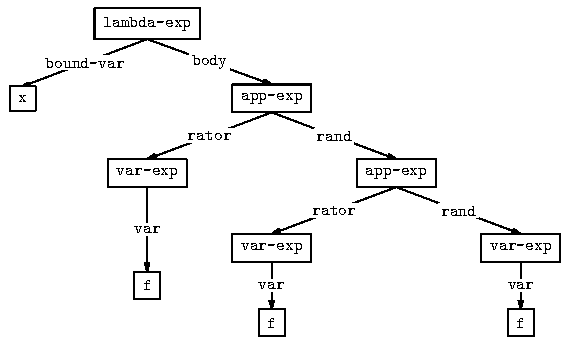
\includegraphics[scale=1.0]{ast.pdf}\end{SCentered}

\caption{\Scribtexttt{(lambda (x) (f (f x)))} 的抽象语法树\label{t:x28elem_x22figx2d2x2e2x22x29}}\end{EoplFigure}

\index{czhou1xiang4yu3fa3@抽象语法|(idxdecorator{}{}}
\index{jzu4ti3yu3fa3@具体语法|(idxdecorator{}{}}
语法通常指定归纳式数据类型的某一具体表示,后者使用前者生成的字符串或值。这种表示
叫做\emph{具体语法} (\emph{concrete syntax}),或\emph{外在} (\emph{external}) 表示。

例如, 指定集合 lambda 演算表达式,用的就是 lambda 演算表
达式的具体语法。我们可以用其他具体语法表示 lambda 演算表达式。例如,可以用

\begin{Subflow}\label{t:x28elem_x22lambdax2d2x22x29}\Iidentity{\begin{align*}\mathit{Lc\mbox{-}exp} &::= \mathit{Identifier} \\
&::= \Scribtexttt{proc }\Iidentity{\mathit{Identifier}}\Scribtexttt{ }\Scribtexttt{={\Stttextmore}}\Scribtexttt{ }\Iidentity{\mathit{Lc\mbox{-}exp}} \\
&::= \Iidentity{\mathit{Lc\mbox{-}exp}}\Scribtexttt{ (}\Iidentity{\mathit{Lc\mbox{-}exp}}\Scribtexttt{)}\end{align*}}

把 lambda 演算表达式定义为另一个字符串集合。\end{Subflow}

为了处理这样的数据,需要将其转换为\emph{内在} (\emph{internal}) 表示。
\Scribtexttt{define{-}datatype} 形式提供了一种简洁的方式来定义这样的内在表示。我们称之
为\emph{抽象语法} (\emph{abstract syntax})。在抽象语法中,不需要存储括号之类的终止符,
因为它们不传达信息。另一方面,我们要确保数据结构足以区分它所表示的 lambda 演算表
达式,并提取出各部分。lc{-}exp的数据类型 \Scribtexttt{lc{-}exp} 助我们轻松实现这些。

\index{czhou1xiang4yu3fa3shu4@抽象语法树|(idxdecorator{}{}}
\index{fzei1zhong1jie2fu2@非终结符|(idxdecorator{}{}}
\index{yzu3fa3sheng1cheng2shi4@语法生成式|(idxdecorator{}{}}
将内在表示形象化为\emph{抽象语法树} (\emph{abstract syntax tree}) 也很不错。
 展示了一棵抽象语法树,它代表数据类型 \Scribtexttt{lc{-}exp} 表示的
lambda 演算表达式 \Scribtexttt{(lambda (x) (f (f x)))}。树的每个内部节点以相应的生成式名
字为标识。树枝以所出现的非终结符名字为标识。叶子对应终止符字符串。

要为某种具体语法设计抽象语法,需要给其中的每个生成式,以及生成式中出现的每个非终
止符命名。很容易将抽象语法写成 \Scribtexttt{define{-}datatype} 声明。我们为每个非终结符添加
一个 \Scribtexttt{define{-}datatype},为每个生成式添加一个变体。
\index{fzei1zhong1jie2fu2@非终结符|)idxdecorator{}{}}
\index{yzu3fa3sheng1cheng2shi4@语法生成式|)idxdecorator{}{}}

 中挑出的内容可以精确表示如下:

\label{t:x28elem_x22lcx2dgrammar2x22x29}\Iidentity{\begin{align*}\mathit{Lc\mbox{-}Exp} &::= \mathit{Identifier} \\[-3pt]
&\mathrel{\phantom{::=}} \fbox{\Scribtexttt{var{-}exp (var)}} \\[5pt]
&::= \normalfont{\Scribtexttt{(lambda (}\Iidentity{\mathit{Identifier}}\Scribtexttt{) }\Iidentity{\mathit{Lc\mbox{-}Exp}}\Scribtexttt{)}} \\[-3pt]
&\mathrel{\phantom{::=}} \fbox{\Scribtexttt{lambda{-}exp (bound{-}var body)}} \\[5pt]
&::= \normalfont{\Scribtexttt{(}\Iidentity{\mathit{Lc\mbox{-}Exp}}\Scribtexttt{ }\Iidentity{\mathit{Lc\mbox{-}Exp}}\Scribtexttt{)}} \\[-3pt]
&\mathrel{\phantom{::=}} \fbox{\Scribtexttt{app{-}exp (rator rand)}}\end{align*}}

本书采用这种表示,同时指明具体语法和抽象语法。
\index{jzu4fa3lei4bie2@句法类别|)idxdecorator{}{}}

具体语法主要供人使用,抽象语法主要供计算机使用,既已区分二者,现在来看看如何将一
种语法转换为另一种。

当具体语法是个字符串集合,推导出对应的抽象语法树可能相当棘手。这一任务
叫做\emph{解析} (\emph{parsing}),由\emph{解析器} (\emph{parser}) 完成。因为写解析器通常比较
麻烦,所以最好借由工具\emph{解析器生成器} (\emph{parser generator}) 完成。
\index{jzie3xi1qi4sheng1cheng2qi4@解析器生成器|idxdecorator{}{}}
\index{jzie3xi1@解析|idxdecorator{}{}}
解析器生成器以一套语法作为输入,产生一个解析器。由于语法是由工具处理的,它们必需
以某种机器能够理解的语言写成,即写语法用的特定领域语言。有很多现成的解析器生成器。
\index{tze4ding4ling3yu4yu3yan2@特定领域语言|idxdecorator{}{}}

\index{jzu4ti3yu3fa3@具体语法|)idxdecorator{}{}}
如果具体语法以列表集合的形式给出,解析过程就会大大简化。比如,
和define{-}datatype \Scribtexttt{define{-}datatype} 的语法类似,
\hyperref[t:x28elem_x22lambdax2d2x22x29]{本节开头}的 lambda 演算表达式指定了一个列表集合。这样,Scheme
过程 \Scribtexttt{read} 会自动把字符串解析为列表和符号。然后,把这些列表结构解析为抽象语
法树就容易多了,就像 \Scribtexttt{parse{-}expression} 这样。

\begin{EoplCodeInset}\index{parseexpression@\textbf{\Scribtexttt{parse{-}expression}}|(idxdecorator{}{}}


\begin{SCodeFlow}\begin{RktBlk}\begin{SingleColumn}\textbf{\Scribtexttt{parse{-}expression}} : \texMathInline{\mathit{SchemeVal} \to \mathit{LcExp}}

\RktPn{(}\RktSym{define}\mbox{\hphantom{\Scribtexttt{x}}}\RktSym{parse{-}expression}

\mbox{\hphantom{\Scribtexttt{xx}}}\RktPn{(}\RktSym{lambda}\mbox{\hphantom{\Scribtexttt{x}}}\RktPn{(}\RktSym{datum}\RktPn{)}

\mbox{\hphantom{\Scribtexttt{xxxx}}}\RktPn{(}\RktSym{cond}

\mbox{\hphantom{\Scribtexttt{xxxxxx}}}\RktPn{(}\RktPn{(}\RktSym{symbol{\hbox{\texttt{?}}}}\mbox{\hphantom{\Scribtexttt{x}}}\RktSym{datum}\RktPn{)}\mbox{\hphantom{\Scribtexttt{x}}}\RktPn{(}\RktSym{var{-}exp}\mbox{\hphantom{\Scribtexttt{x}}}\RktSym{datum}\RktPn{)}\RktPn{)}

\mbox{\hphantom{\Scribtexttt{xxxxxx}}}\RktPn{(}\RktPn{(}\RktSym{pair{\hbox{\texttt{?}}}}\mbox{\hphantom{\Scribtexttt{x}}}\RktSym{datum}\RktPn{)}

\mbox{\hphantom{\Scribtexttt{xxxxxxxx}}}\RktPn{(}\RktSym{if}\mbox{\hphantom{\Scribtexttt{x}}}\RktPn{(}\RktSym{eqv{\hbox{\texttt{?}}}}\mbox{\hphantom{\Scribtexttt{x}}}\RktPn{(}\RktSym{car}\mbox{\hphantom{\Scribtexttt{x}}}\RktSym{datum}\RktPn{)}\mbox{\hphantom{\Scribtexttt{x}}}\RktVal{{\textquotesingle}}\RktVal{lambda}\RktPn{)}

\mbox{\hphantom{\Scribtexttt{xxxxxxxxxx}}}\RktPn{(}\RktSym{lambda{-}exp}

\mbox{\hphantom{\Scribtexttt{xxxxxxxxxxxx}}}\RktPn{(}\RktSym{car}\mbox{\hphantom{\Scribtexttt{x}}}\RktPn{(}\RktSym{cadr}\mbox{\hphantom{\Scribtexttt{x}}}\RktSym{datum}\RktPn{)}\RktPn{)}

\mbox{\hphantom{\Scribtexttt{xxxxxxxxxxxx}}}\RktPn{(}\RktSym{parse{-}expression}\mbox{\hphantom{\Scribtexttt{x}}}\RktPn{(}\RktSym{caddr}\mbox{\hphantom{\Scribtexttt{x}}}\RktSym{datum}\RktPn{)}\RktPn{)}\RktPn{)}

\mbox{\hphantom{\Scribtexttt{xxxxxxxxxx}}}\RktPn{(}\RktSym{app{-}exp}

\mbox{\hphantom{\Scribtexttt{xxxxxxxxxxxx}}}\RktPn{(}\RktSym{parse{-}expression}\mbox{\hphantom{\Scribtexttt{x}}}\RktPn{(}\RktSym{car}\mbox{\hphantom{\Scribtexttt{x}}}\RktSym{datum}\RktPn{)}\RktPn{)}

\mbox{\hphantom{\Scribtexttt{xxxxxxxxxxxx}}}\RktPn{(}\RktSym{parse{-}expression}\mbox{\hphantom{\Scribtexttt{x}}}\RktPn{(}\RktSym{cadr}\mbox{\hphantom{\Scribtexttt{x}}}\RktSym{datum}\RktPn{)}\RktPn{)}\RktPn{)}\RktPn{)}\RktPn{)}

\mbox{\hphantom{\Scribtexttt{xxxxxx}}}\RktPn{(}\RktSym{else}\mbox{\hphantom{\Scribtexttt{x}}}\RktPn{(}\RktSym{report{-}invalid{-}concrete{-}syntax}\mbox{\hphantom{\Scribtexttt{x}}}\RktSym{datum}\RktPn{)}\RktPn{)}\RktPn{)}\RktPn{)}\RktPn{)}\end{SingleColumn}\end{RktBlk}\end{SCodeFlow}

\noindent \index{parseexpression@\textbf{\Scribtexttt{parse{-}expression}}|)idxdecorator{}{}}\end{EoplCodeInset}

\index{unparselcexp@\textbf{\Scribtexttt{unparse{-}lc{-}exp}}|(idxdecorator{}{}}
通常,很容易把抽象语法树重新转换为列表{-}符号表示。我们这样做了,Scheme 的打印过程
就会将其显示为列表形式的具体语法。这由 \Scribtexttt{unparse{-}lc{-}exp} 完成:

\begin{EoplCodeInset}\begin{SCodeFlow}\begin{RktBlk}\begin{SingleColumn}\textbf{\Scribtexttt{unparse{-}lc{-}exp}} : \texMathInline{\mathit{LcExp} \to \mathit{SchemeVal}}

\RktPn{(}\RktSym{define}\mbox{\hphantom{\Scribtexttt{x}}}\RktSym{unparse{-}lc{-}exp}

\mbox{\hphantom{\Scribtexttt{xx}}}\RktPn{(}\RktSym{lambda}\mbox{\hphantom{\Scribtexttt{x}}}\RktPn{(}\RktSym{exp}\RktPn{)}

\mbox{\hphantom{\Scribtexttt{xxxx}}}\RktPn{(}\RktSym{cases}\mbox{\hphantom{\Scribtexttt{x}}}\RktSym{lc{-}exp}\mbox{\hphantom{\Scribtexttt{x}}}\RktSym{exp}

\mbox{\hphantom{\Scribtexttt{xxxxxx}}}\RktPn{(}\RktSym{var{-}exp}\mbox{\hphantom{\Scribtexttt{x}}}\RktPn{(}\RktSym{var}\RktPn{)}\mbox{\hphantom{\Scribtexttt{x}}}\RktSym{var}\RktPn{)}

\mbox{\hphantom{\Scribtexttt{xxxxxx}}}\RktPn{(}\RktSym{lambda{-}exp}

\mbox{\hphantom{\Scribtexttt{xxxxxxxx}}}\RktPn{(}\RktSym{bound{-}var}\mbox{\hphantom{\Scribtexttt{x}}}\RktSym{body}\RktPn{)}

\mbox{\hphantom{\Scribtexttt{xxxxxxxx}}}\RktPn{(}\RktSym{list}\mbox{\hphantom{\Scribtexttt{x}}}\RktVal{{\textquotesingle}}\RktVal{lambda}

\mbox{\hphantom{\Scribtexttt{xxxxxxxxxx}}}\RktPn{(}\RktSym{list}\mbox{\hphantom{\Scribtexttt{x}}}\RktSym{bound{-}var}\RktPn{)}

\mbox{\hphantom{\Scribtexttt{xxxxxxxxxx}}}\RktPn{(}\RktSym{unparse{-}lc{-}exp}\mbox{\hphantom{\Scribtexttt{x}}}\RktSym{body}\RktPn{)}\RktPn{)}\RktPn{)}

\mbox{\hphantom{\Scribtexttt{xxxxxx}}}\RktPn{(}\RktSym{app{-}exp}

\mbox{\hphantom{\Scribtexttt{xxxxxxxx}}}\RktPn{(}\RktSym{rator}\mbox{\hphantom{\Scribtexttt{x}}}\RktSym{rand}\RktPn{)}

\mbox{\hphantom{\Scribtexttt{xxxxxxxx}}}\RktPn{(}\RktSym{list}\mbox{\hphantom{\Scribtexttt{x}}}\RktPn{(}\RktSym{unparse{-}lc{-}exp}\mbox{\hphantom{\Scribtexttt{x}}}\RktSym{rator}\RktPn{)}

\mbox{\hphantom{\Scribtexttt{xxxxxxxxxx}}}\RktPn{(}\RktSym{unparse{-}lc{-}exp}\mbox{\hphantom{\Scribtexttt{x}}}\RktSym{rand}\RktPn{)}\RktPn{)}\RktPn{)}\RktPn{)}\RktPn{)}\RktPn{)}\end{SingleColumn}\end{RktBlk}\end{SCodeFlow}

\noindent \index{czhou1xiang4yu3fa3@抽象语法|)idxdecorator{}{}}
\index{czhou1xiang4yu3fa3shu4@抽象语法树|)idxdecorator{}{}}
\index{Lambdabziao3da2shi4LcExp@Lambda 表达式 (LcExp)!czhou1xiang4vs.ju4ti3yu3fa3@抽象 vs. 具体语法|)idxdecorator{}{}}
\index{unparselcexp@\textbf{\Scribtexttt{unparse{-}lc{-}exp}}|)idxdecorator{}{}}\end{EoplCodeInset}

\begin{EoplExercise}\label{t:x28elem_x22ex2x2e27x22x29}\texMathInline{\textnormal{[}{\star}\textnormal{]}}\mbox{\hphantom{\Scribtexttt{x}}}\index{Lambdabziao3da2shi4LcExp@Lambda 表达式 (LcExp)|(idxdecorator{}{}}
画出下面 lambda 演算表达式的抽象语法树:

\begin{EoplCodeInset}\begin{SCodeFlow}\begin{RktBlk}\begin{SingleColumn}\RktPn{(}\RktPn{(}\RktSym{lambda}\mbox{\hphantom{\Scribtexttt{x}}}\RktPn{(}\RktSym{a}\RktPn{)}\mbox{\hphantom{\Scribtexttt{x}}}\RktPn{(}\RktSym{a}\mbox{\hphantom{\Scribtexttt{x}}}\RktSym{b}\RktPn{)}\RktPn{)}\mbox{\hphantom{\Scribtexttt{x}}}\RktSym{c}\RktPn{)}

\mbox{\hphantom{\Scribtexttt{x}}}

\RktPn{(}\RktSym{lambda}\mbox{\hphantom{\Scribtexttt{x}}}\RktPn{(}\RktSym{x}\RktPn{)}

\mbox{\hphantom{\Scribtexttt{xx}}}\RktPn{(}\RktSym{lambda}\mbox{\hphantom{\Scribtexttt{x}}}\RktPn{(}\RktSym{y}\RktPn{)}

\mbox{\hphantom{\Scribtexttt{xxxx}}}\RktPn{(}\RktPn{(}\RktSym{lambda}\mbox{\hphantom{\Scribtexttt{x}}}\RktPn{(}\RktSym{x}\RktPn{)}

\mbox{\hphantom{\Scribtexttt{xxxxxxx}}}\RktPn{(}\RktSym{x}\mbox{\hphantom{\Scribtexttt{x}}}\RktSym{y}\RktPn{)}\RktPn{)}

\mbox{\hphantom{\Scribtexttt{xxxxx}}}\RktSym{x}\RktPn{)}\RktPn{)}\RktPn{)}\end{SingleColumn}\end{RktBlk}\end{SCodeFlow}\end{EoplCodeInset}\end{EoplExercise}

\begin{EoplExercise}\label{t:x28elem_x22ex2x2e28x22x29}\texMathInline{\textnormal{[}{\star}\textnormal{]}}\mbox{\hphantom{\Scribtexttt{x}}}\index{unparselcexp@\textbf{\Scribtexttt{unparse{-}lc{-}exp}}|idxdecorator{}{}}
写出反向解析器,将lc{-}exp的抽象语法转换为符合本节第二个语法
(lc{-}grammar2)的字符串。\end{EoplExercise}

\begin{EoplExercise}\label{t:x28elem_x22ex2x2e29x22x29}\texMathInline{\textnormal{[}{\star}\textnormal{]}}\mbox{\hphantom{\Scribtexttt{x}}}\index{kze4lai2ni2jia1hao4@克莱尼加号|(idxdecorator{}{}}
\index{kze4lai2ni2xing1hao4bi4bao1@克莱尼星号(闭包)|(idxdecorator{}{}}
\index{parseexpression@\textbf{\Scribtexttt{parse{-}expression}}|(idxdecorator{}{}}
当具体语法使用克莱尼星号或加号(kleene{-}star)时,生成抽象语法树时最好
使用相应子树的\emph{列表}。例如,如果 lambda 演算表达式的语法为:

\begin{Subflow}\Iidentity{\begin{align*}\mathit{Lc\mbox{-}Exp} &::= \mathit{Identifier} \\[-3pt]
                       &\mathrel{\phantom{::=}} \fbox{\Scribtexttt{var{-}exp (var)}} \\[5pt]
                       &::= \normalfont{\Scribtexttt{(lambda (}\Iidentity{\{\mathit{Identifier}\}^{*}}\Scribtexttt{) }\Iidentity{\mathit{Lc\mbox{-}Exp}}\Scribtexttt{)}} \\[-3pt]
                       &\mathrel{\phantom{::=}} \fbox{\Scribtexttt{lambda{-}exp (bound{-}vars body)}} \\[5pt]
                       &::= \normalfont{\Scribtexttt{(}\Iidentity{\mathit{Lc\mbox{-}Exp}}\Scribtexttt{ }\Iidentity{\{\mathit{Lc\mbox{-}Exp}\}^{*}}\Scribtexttt{)}} \\[-3pt]
                       &\mathrel{\phantom{::=}} \fbox{\Scribtexttt{app{-}exp (rator rands)}}\end{align*}}

那么字段 \Scribtexttt{bound{-}vars} 的谓词可写作 \Scribtexttt{(list{-}of identifier{\hbox{\texttt{?}}})},\Scribtexttt{rands} 的
谓词可写作 \Scribtexttt{(list{-}of lc{-}exp{\hbox{\texttt{?}}})}。以这种方式写出该语法的 \Scribtexttt{define{-}datatype}
和解析器。
\index{kze4lai2ni2jia1hao4@克莱尼加号|)idxdecorator{}{}}
\index{kze4lai2ni2xing1hao4bi4bao1@克莱尼星号(闭包)|)idxdecorator{}{}}\end{Subflow}\end{EoplExercise}

\begin{EoplExercise}\label{t:x28elem_x22ex2x2e30x22x29}\texMathInline{\textnormal{[}{\star}{\star}\textnormal{]}}\mbox{\hphantom{\Scribtexttt{x}}}上面定义的过程 \Scribtexttt{parse{-}expression} 很不可靠:它检查不到某些可能的语法错误,例
如 \Scribtexttt{(a b c)},并且因其他表达式终止时给不出恰当的错误信息,如 \Scribtexttt{(lambda)}。
修改一下,使之更健壮,可接受任何s{-}exp,并且对不表示 lambda 演算表达式的 s{-}exp 给
出恰当的错误信息。
\index{Lambdabziao3da2shi4LcExp@Lambda 表达式 (LcExp)|)idxdecorator{}{}}
\index{parseexpression@\textbf{\Scribtexttt{parse{-}expression}}|)idxdecorator{}{}}\end{EoplExercise}

\begin{EoplExercise}\label{t:x28elem_x22ex2x2e31x22x29}\texMathInline{\textnormal{[}{\star}{\star}\textnormal{]}}\mbox{\hphantom{\Scribtexttt{x}}}\index{qzian2zhui4lie4biao3@前缀列表 (\texMathInline{\mathit{Prefix\mbox{-}list}})|(idxdecorator{}{}}
有时,把具体语法定义为括号包围的符号和整数序列很有用。例如,可以把
集合\emph{前缀列表} (\emph{prefix list}) 定义为:

\begin{Subflow}\Iidentity{\begin{align*}\mathit{Prefix\mbox{-}list} &::= \Scribtexttt{(}\Iidentity{\mathit{Prefix\mbox{-}exp}}\Scribtexttt{)} \\
\mathit{Prefix\mbox{-}exp}  &::= \mathit{Int} \\
                            &::= \Scribtexttt{{-} }\Iidentity{\mathit{Prefix\mbox{-}exp}}\Scribtexttt{ }\Iidentity{\mathit{Prefix\mbox{-}exp}}\end{align*}}

那么 \Scribtexttt{({-} {-} 3 2 {-} 4 {-} 12 7)}是一个合法的前缀列表。有时为纪念其发明者Jan
{\L}ukasiewicz,称之为\emph{波兰前缀表示法} (\emph{Polish prefix notation})。写一个
解析器,将前缀列表表示法转换为抽象语法:
\index{LukasiewiczJan@{\L}ukasiewicz, Jan|idxdecorator{}{}}
\index{bzo1lan2qian2zhui4biao3shi4fa3@波兰前缀表示法|idxdecorator{}{}}

\begin{EoplCodeInset}\begin{SCodeFlow}\begin{RktBlk}\begin{SingleColumn}\RktPn{(}\RktSym{define{-}datatype}\mbox{\hphantom{\Scribtexttt{x}}}\RktSym{prefix{-}exp}\mbox{\hphantom{\Scribtexttt{x}}}\RktSym{prefix{-}exp{\hbox{\texttt{?}}}}

\mbox{\hphantom{\Scribtexttt{xx}}}\RktPn{(}\RktSym{const{-}exp}

\mbox{\hphantom{\Scribtexttt{xxx}}}\RktPn{(}\RktSym{num}\mbox{\hphantom{\Scribtexttt{x}}}\RktSym{integer{\hbox{\texttt{?}}}}\RktPn{)}\RktPn{)}

\mbox{\hphantom{\Scribtexttt{xx}}}\RktPn{(}\RktSym{diff{-}exp}

\mbox{\hphantom{\Scribtexttt{xxx}}}\RktPn{(}\RktSym{operand1}\mbox{\hphantom{\Scribtexttt{x}}}\RktSym{prefix{-}exp{\hbox{\texttt{?}}}}\RktPn{)}

\mbox{\hphantom{\Scribtexttt{xxx}}}\RktPn{(}\RktSym{operand2}\mbox{\hphantom{\Scribtexttt{x}}}\RktSym{prefix{-}exp{\hbox{\texttt{?}}}}\RktPn{)}\RktPn{)}\RktPn{)}\end{SingleColumn}\end{RktBlk}\end{SCodeFlow}\end{EoplCodeInset}

使上例与这几个构造器生成相同抽象语法树:

\begin{EoplCodeInset}\begin{SCodeFlow}\begin{RktBlk}\begin{SingleColumn}\RktPn{(}\RktSym{diff{-}exp}

\mbox{\hphantom{\Scribtexttt{x}}}\RktPn{(}\RktSym{diff{-}exp}

\mbox{\hphantom{\Scribtexttt{xx}}}\RktPn{(}\RktSym{const{-}exp}\mbox{\hphantom{\Scribtexttt{x}}}\RktVal{3}\RktPn{)}

\mbox{\hphantom{\Scribtexttt{xx}}}\RktPn{(}\RktSym{const{-}exp}\mbox{\hphantom{\Scribtexttt{x}}}\RktVal{2}\RktPn{)}\RktPn{)}

\mbox{\hphantom{\Scribtexttt{x}}}\RktPn{(}\RktSym{diff{-}exp}

\mbox{\hphantom{\Scribtexttt{xx}}}\RktPn{(}\RktSym{const{-}exp}\mbox{\hphantom{\Scribtexttt{x}}}\RktVal{4}\RktPn{)}

\mbox{\hphantom{\Scribtexttt{xx}}}\RktPn{(}\RktSym{diff{-}exp}

\mbox{\hphantom{\Scribtexttt{xxx}}}\RktPn{(}\RktSym{const{-}exp}\mbox{\hphantom{\Scribtexttt{x}}}\RktVal{12}\RktPn{)}

\mbox{\hphantom{\Scribtexttt{xxx}}}\RktPn{(}\RktSym{const{-}exp}\mbox{\hphantom{\Scribtexttt{x}}}\RktVal{7}\RktPn{)}\RktPn{)}\RktPn{)}\RktPn{)}\end{SingleColumn}\end{RktBlk}\end{SCodeFlow}\end{EoplCodeInset}

提示:想想如何写一个过程,取一列表,产生一个 \Scribtexttt{prefix{-}exp} 和列表剩余元素组成
的列表。
\index{qzian2zhui4lie4biao3@前缀列表 (\texMathInline{\mathit{Prefix\mbox{-}list}})|)idxdecorator{}{}}\end{Subflow}\end{EoplExercise}

\sectionNewpage

\Ssection{表达式}{表达式}\label{t:x28part_x22exprx22x29}

本章研究变量绑定及其作用域。我们用一系列小型语言解释这些概念。我们为这些语言写出
规范,遵照\ChapRefLocal{t:x28part_x22isdx22x29}{1}{归纳式数据集}的解释器秘方实现其解释器。我们的规范和解释器取一
名为\emph{环境} (\emph{environment}) 的上下文参数,以记录待求值的表达式中各个变量的含
义。

\Ssubsection{规范和实现策略}{规范和实现策略}\label{t:x28part_x22s3x2e1x22x29}

\index{yzu3yan2chu4li3qi4@语言处理器|(idxdecorator{}{}}
我们的规范包含若干断言,形如:


\noindent \begin{Subflow}\texMathDisplay{\Scribtexttt{(value{-}of }\texMathInline{exp}\Scribtexttt{ }\texMathInline{\rho}\Scribtexttt{)} = val}

意为在环境 \texMathInline{\rho} 中,表达式 \texMathInline{exp} 的值应为 \texMathInline{val}。我们像\ChapRefLocal{t:x28part_x22isdx22x29}{1}{归纳式数据集}那样,
写出推理规则和方程,以便推导出这样的断言。我们手写规则和方程,找出某些表达式的期
望值。\end{Subflow}

\index{czhou1xiang4yu3fa3shu4@抽象语法树|(idxdecorator{}{}}而我们的目标是写出程序,
\index{bzei4ding4yu3yan2@被定语言|idxdecorator{}{}}
\index{dzing4yi4yu3yan2@定义语言|idxdecorator{}{}}
\index{yzuan2yu3yan2@源语言|idxdecorator{}{}}
实现语言。概况如 所示。首先是程序,由我们要实现的语言写出。
这叫做\emph{源语言} (\emph{source language}) 或\emph{被定语言} (\emph{defined language})。前
端接收程序文本(由源语言写成的程序),将其转化为抽象语法树,然后将语法树传给解释
器。解释器是一程序,它查看一段数据结构,根据结构执行一些动作。当然,解释器自身也
由某种语言写成。我们把那种语言叫做\emph{实现语言} (\emph{implementation language})
\index{szhi2xian4yu3yan2@实现语言|idxdecorator{}{}}
或\emph{定义语言} (\emph{defining language})。我们的大多数实现都遵照这种方式。

\index{bzian1yi4qi4@编译器|idxdecorator{}{}}
另一种常见的组织方式如 所示。其中,编译器替代了解释器,将
抽象语法树翻译为另一种语言(称为\emph{目标语言} (\emph{target language}))写成的
程序,然后执行。目标语言可能像 那样,由一个解释器执行,也
可能翻译成更底层的语言执行。
\index{mzu4biao1yu3yan2@目标语言|idxdecorator{}{}}

通常,目标语言是一种机器语言,由硬件解释。但目标语言也可能是一种特定用途的语言,
比原本的语言简单,为它写一个解释器相对容易。这样,程序可以编译一次,然后在多种不
同的硬件平台上执行。出于历史原因,常称这样的目标语言为\emph{字节码} (\emph{byte
code}),称其解释器称为\emph{虚拟机} (\emph{virtual machine})。
\index{zzi4jie2ma3@字节码|idxdecorator{}{}}
\index{jzi1qi4yu3yan2@机器语言|idxdecorator{}{}}
\index{xzu1ni3ji1@虚拟机|idxdecorator{}{}}

编译器常常分为两部分:\emph{分析器} (\emph{analyzer}),尝试推断关于程序的有效信
息;\emph{翻译器} (\emph{translator}),执行翻译,可能用到来自分析器的信息。这些
阶段既能用推理规则指定,也能用专写规范的语言指定。然后是实现。
\ChapRefLocal{t:x28part_x22cpsx22x29}{6}{续文传递风格}和\ChapRefLocal{t:x28part_x22typesx22x29}{7}{类型}探讨了一些简单的分析器和翻译器。

\index{jzie3xi1@解析|(idxdecorator{}{}}
不论采用哪种实现策略,我们都需要一个\emph{前端} (\emph{front end}),将程序转换为
抽象语法树。因为程序只是字符串,我们的前端要将这些字符组成有意义的单元。分组通常
分为两个阶段:\emph{扫描} (\emph{scanning}) 和\emph{解析} (\emph{parsing})。
\index{szao3miao2@扫描|idxdecorator{}{}}

扫描就是将字符序列分为单词、数字、标点、注释等等。这些单元叫做\emph{词条} (\emph{lexical
item})、\emph{词素} (\emph{lexeme})、或者最常见的\emph{词牌} (\emph{token})。把程序分
为词牌的方式叫做语言的\emph{词法规范} (\emph{lexical specification})。扫描器取一字符序
列,生成词牌序列。
\index{czi2fa3gui1fan4@词法规范|idxdecorator{}{}}
\index{czi2pai2@词牌|idxdecorator{}{}}

解析就是将词牌序列组成有层次的语法结构,如表达式、语句和块。这就像用从句组织(或
称图解\NoteBox{\NoteContent{西方有diagram sentence之说,以树状图表示句子结构,如我国中学生学习英
文之主、谓、宾。{---}{---}\emph{译注}}})句子。我们称之为语言的\emph{句法} (\emph{syntactic})
或\emph{语法} (\emph{grammatical}) 结构。解析器取一词牌序列(由扫描器给出),生成一棵
抽象语法树。\index{czhou1xiang4yu3fa3shu4@抽象语法树|)idxdecorator{}{}}

\index{jzie3xi1qi4sheng1cheng2qi4@解析器生成器|(idxdecorator{}{}}
设计前端的标准方式是使用\emph{解析器生成器} (\emph{parser generator})。解析器生
成器是一程序,取一词法规范和语法,生成一个扫描器和解析器。

\begin{EoplFigure}[!ht]
 

\noindent \begin{EoplSubfigure}\begin{SCentered}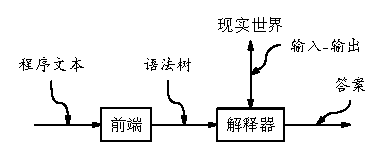
\includegraphics[scale=1.0]{exe-via-interpreter.pdf}\end{SCentered}

\caption{由解释器执行\label{t:x28elem_x22figx2d3x2e1x2dax22x29}}\end{EoplSubfigure}

\begin{EoplSubfigure}\begin{SCentered}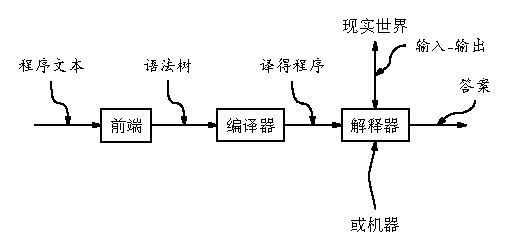
\includegraphics[scale=1.0]{exe-via-compiler.pdf}\end{SCentered}

\caption{由编译器执行\label{t:x28elem_x22figx2d3x2e1x2dbx22x29}}\end{EoplSubfigure}

\caption{语言处理系统块状图\label{t:x28elem_x22figx2d3x2e1x22x29}}\end{EoplFigure}

大多数主流语言都有解析器生成系统。如果没有解析器生成器,或者没有合适的,可以手写
扫描器和解析器。编译器教材描述了这一过程。本书使用的解析技术及相关语法设计从简,
专为满足我们的需求。
\index{jzie3xi1qi4sheng1cheng2qi4@解析器生成器|)idxdecorator{}{}}

另一种方式是忽略具体语法的细节,把表达式写成列表结构,
就像\SecRefLocal{t:x28part_x22s2x2e5x22x29}{2.5}{抽象语法及其表示}和ex2.31中,处理 lambda 演算表达式那样。
\index{yzu3yan2chu4li3qi4@语言处理器|)idxdecorator{}{}}
\index{jzie3xi1@解析|)idxdecorator{}{}}

\Ssubsection{LET:一门简单语言}{LET:一门简单语言}\label{t:x28part_x22s3x2e2x22x29}

\index{LET|(idxdecorator{}{}}
我们先来定义一种非常简单的语言,根据它最有趣的特性,将其命名为 LET。

\Ssubsubsection{定义语法}{定义语法}\label{t:x28part_x22s3x2e2x2e1x22x29}

 展示了我们这门简单语言的语法。在这种语言中,程序只能是一个表达式。表达式是
个整数常量、差值表达式、判零表达式、条件表达式、变量、或 \Scribtexttt{let} 表达式。

这里是本门语言写成的一个简单表达式,及其抽象语法表示。

\begin{EoplCodeInset}\begin{SCodeFlow}\begin{RktBlk}\begin{SingleColumn}\RktPn{(}\RktSym{scan\&parse}\mbox{\hphantom{\Scribtexttt{x}}}\RktVal{"{-}(55, {-}(x,11))"}\RktPn{)}

\RktVal{\#}\RktVal{(}\RktVal{struct{\hbox{\texttt{:}}}a{-}program}

\mbox{\hphantom{\Scribtexttt{xx}}}\RktVal{\#}\RktVal{(}\RktVal{struct{\hbox{\texttt{:}}}diff{-}exp}

\mbox{\hphantom{\Scribtexttt{xxxx}}}\RktVal{\#}\RktVal{(}\RktVal{struct{\hbox{\texttt{:}}}const{-}exp}\mbox{\hphantom{\Scribtexttt{x}}}\RktVal{55}\RktVal{)}

\mbox{\hphantom{\Scribtexttt{xxxx}}}\RktVal{\#}\RktVal{(}\RktVal{struct{\hbox{\texttt{:}}}diff{-}exp}

\mbox{\hphantom{\Scribtexttt{xxxxxx}}}\RktVal{\#}\RktVal{(}\RktVal{struct{\hbox{\texttt{:}}}var{-}exp}\mbox{\hphantom{\Scribtexttt{x}}}\RktVal{x}\RktVal{)}

\mbox{\hphantom{\Scribtexttt{xxxxxx}}}\RktVal{\#}\RktVal{(}\RktVal{struct{\hbox{\texttt{:}}}const{-}exp}\mbox{\hphantom{\Scribtexttt{x}}}\RktVal{11}\RktVal{)}\RktVal{)}\RktVal{)}\RktVal{)}\end{SingleColumn}\end{RktBlk}\end{SCodeFlow}\end{EoplCodeInset}

\begin{EoplFigure}[!ht]
\hspace*{\fill}\\
\Iidentity{\begin{align*}\mathit{Program} &::= \mathit{Expression} \\[-3pt]
  &\mathrel{\phantom{::=}} \fbox{\Scribtexttt{a{-}program (exp1)}} \\[5pt]
\mathit{Expression} &::= \mathit{Number} \\[-3pt]
  &\mathrel{\phantom{::=}} \fbox{\Scribtexttt{const{-}exp (num)}} \\[5pt]
\mathit{Expression} &::= \Scribtexttt{({-} }\Iidentity{\mathit{Expression}}\Scribtexttt{ , }\Iidentity{\mathit{Expression}}\Scribtexttt{)} \\[-3pt]
  &\mathrel{\phantom{::=}} \fbox{\Scribtexttt{diff{-}exp (exp1 exp2)}} \\[5pt]
\mathit{Expression} &::= \Scribtexttt{(zero{\hbox{\texttt{?}}} }\Iidentity{\mathit{Expression}}\Scribtexttt{)} \\[-3pt]
  &\mathrel{\phantom{::=}} \fbox{\Scribtexttt{zero{\hbox{\texttt{?}}}{-}exp (exp1)}} \\[5pt]
\mathit{Expression} &::= \Scribtexttt{if }\Iidentity{\mathit{Expression}}\Scribtexttt{ then }\Iidentity{\mathit{Expression}}\Scribtexttt{ else }\Iidentity{\mathit{Expression}} \\[-3pt]
  &\mathrel{\phantom{::=}} \fbox{\Scribtexttt{if{-}exp (exp1 exp2 exp3)}} \\[5pt]
\mathit{Expression} &::= \mathit{Identifier} \\[-3pt]
  &\mathrel{\phantom{::=}} \fbox{\Scribtexttt{var{-}exp (var)}} \\[5pt]
\mathit{Expression} &::= \Scribtexttt{let }\Iidentity{\mathit{Identifier}}\Scribtexttt{ = }\Iidentity{\mathit{Expression}}\Scribtexttt{ in }\Iidentity{\mathit{Expression}} \\[-3pt]
  &\mathrel{\phantom{::=}} \fbox{\Scribtexttt{let{-}exp (var exp1 body)}}\end{align*}}

\caption{LET语言的语法\label{t:x28elem_x22figx2d3x2e2x22x29}}\end{EoplFigure}

\Ssubsubsection{定义值}{定义值}\label{t:x28part_x22s3x2e2x2e2x22x29}

任何编程语言的规范之中,最重要的一部分就是语言能处理的值的集合。每种语言至少有两
个这样的集合:\emph{表达值} (\emph{expressed values}) 和\emph{指代值} (\emph{denoted values})。
\index{zzhi3dai4zhi2@指代值|idxdecorator{}{}}
\index{bziao3da2zhi2@表达值|idxdecorator{}{}}
表达值是指表达式可能的取值,指代值是指可以绑定到变量的值。

本章的语言中,表达值和指代值总是相同。它们是:

\begin{Subflow}\label{t:x28elem_x22passx2dbyx2dvaluex22x29}\Iidentity{\begin{align*}\mathit{ExpVal} &= \mathit{Int} + \mathit{Bool} \\
\mathit{DenVal} &= \mathit{Int} + \mathit{Bool}\end{align*}}

\ChapRefLocal{t:x28part_x22statex22x29}{4}{状态}展示表达值和指代值不同的语言。\end{Subflow}

要使用这个定义,我们要有表达值数据类型的接口。我们有这几个接口:

\begin{EoplCodeInset}\begin{SVerbatim}\begin{SingleColumn}\textbf{\Scribtexttt{num{-}val}}\Scribtexttt{}\mbox{\hphantom{\Scribtexttt{x}}}\Scribtexttt{}\texMathInline{: \mathit{Int} \to \mathit{ExpVal}}\Scribtexttt{}

\Scribtexttt{}\textbf{\Scribtexttt{bool{-}val}}\Scribtexttt{}\mbox{\hphantom{\Scribtexttt{x}}}\Scribtexttt{}\texMathInline{: \mathit{Bool} \to \mathit{ExpVal}}\Scribtexttt{}

\Scribtexttt{}\textbf{\Scribtexttt{expval{-}{\Stttextmore}num}}\Scribtexttt{}\mbox{\hphantom{\Scribtexttt{x}}}\Scribtexttt{}\texMathInline{: \mathit{ExpVal} \to \mathit{Int}}\Scribtexttt{}

\Scribtexttt{}\textbf{\Scribtexttt{expval{-}{\Stttextmore}bool}}\Scribtexttt{}\mbox{\hphantom{\Scribtexttt{x}}}\Scribtexttt{}\texMathInline{: \mathit{ExpVal} \to \mathit{Bool}}\end{SingleColumn}\end{SVerbatim}\end{EoplCodeInset}

我们假定,当传给 \Scribtexttt{expval{-}{\Stttextmore}num} 的参数不是整数值,或传给 \Scribtexttt{expval{-}{\Stttextmore}bool} 的
参数不是布尔值时,二者行为未定义。

\Ssubsubsection{环境}{环境}\label{t:x28part_x22s3x2e2x2e3x22x29}

\index{hzuan2jing4@环境|(idxdecorator{}{}}
若要求取表达式的值,我们得知道每个变量的值。我们靠环境记录这些值,就像\SecRefLocal{t:x28part_x22s2x2e2x22x29}{2.2}{数据类型的表示策略}那样。

环境是一函数,定义域为变量的有限集合,值域为指代值。我们用一些缩写表示环境。

\begin{itemize}\atItemizeStart

\item \texMathInline{\rho} 表示任一环境。

\item \texMathInline{\textnormal{[]}} 表示空环境。

\item \texMathInline{\text{[}var = val\text{]}\rho} 表示 \Scribtexttt{(extend{-}env }\texMathInline{var}\Scribtexttt{ }\texMathInline{val}\Scribtexttt{
}\texMathInline{\rho}\Scribtexttt{)}。

\item \texMathInline{\text{[}var_1 = val_1, var_2 = val2\text{]}\rho} 是 \texMathInline{var_1 =
val_1(\text{[}var_2 = val_2\text{]}\rho)} 的缩写,其余同理。

\item \texMathInline{\text{[}var_1 = val_1, var_2 = val2,\dots\text{]}} 表示的环境中,
\texMathInline{var_1} 的值为 \texMathInline{val_1},其余同理。\end{itemize}

我们偶尔用不同缩进表示复杂环境,以便阅读。例如,我们可能把

\begin{Subflow}\begin{EoplCodeInset}\begin{SCodeFlow}\begin{RktBlk}\begin{SingleColumn}\RktPn{(}\RktSym{extend{-}env}\mbox{\hphantom{\Scribtexttt{x}}}\RktVal{{\textquotesingle}}\RktVal{x}\mbox{\hphantom{\Scribtexttt{x}}}\RktVal{3}

\mbox{\hphantom{\Scribtexttt{xx}}}\RktPn{(}\RktSym{extend{-}env}\mbox{\hphantom{\Scribtexttt{x}}}\RktVal{{\textquotesingle}}\RktVal{y}\mbox{\hphantom{\Scribtexttt{x}}}\RktVal{7}

\mbox{\hphantom{\Scribtexttt{xxxx}}}\RktPn{(}\RktSym{extend{-}env}\mbox{\hphantom{\Scribtexttt{x}}}\RktVal{{\textquotesingle}}\RktVal{u}\mbox{\hphantom{\Scribtexttt{x}}}\RktVal{5}\mbox{\hphantom{\Scribtexttt{x}}}\texMathInline{\rho}\RktPn{)}\RktPn{)}\RktPn{)}\end{SingleColumn}\end{RktBlk}\end{SCodeFlow}\end{EoplCodeInset}

缩写为

\begin{EoplCodeInset}\begin{SCodeFlow}\begin{RktBlk}\begin{SingleColumn}\RktPn{[}\RktSym{x=3}\RktPn{]}

\mbox{\hphantom{\Scribtexttt{x}}}\RktPn{[}\RktSym{y=7}\RktPn{]}

\mbox{\hphantom{\Scribtexttt{xx}}}\RktPn{[}\RktSym{u=5}\RktPn{]}\texMathInline{\rho}\end{SingleColumn}\end{RktBlk}\end{SCodeFlow}\end{EoplCodeInset}

\noindent \index{hzuan2jing4@环境|)idxdecorator{}{}}\end{Subflow}

\Ssubsubsection{定义表达式的行为}{定义表达式的行为}\label{t:x28part_x22s3x2e2x2e4x22x29}

\index{czha4zhi2biao3da2shi4@差值表达式|(idxdecorator{}{}}
\index{bziao3da2shi4@表达式!LET|(idxdecorator{}{}}
\index{valueof@\textbf{\Scribtexttt{value{-}of}}!LET@LET|(idxdecorator{}{}}
我们语言中的六种表达式各对应一个左边为 \texMathInline{\mathit{Expression}} 的生成式。表达式
接口包含七个过程,六个是构造器,一个是观测器。我们用 \texMathInline{\mathit{ExpVal}} 表示表
达值的集合。

\begin{EoplCodeInset}\begin{SVerbatim}\begin{SingleColumn}\Scribtexttt{构造器:}

\Scribtexttt{}\mbox{\hphantom{\Scribtexttt{x}}}

\Scribtexttt{}\textbf{\Scribtexttt{const{-}exp}}\Scribtexttt{{\hbox{\texttt{:}}} }\texMathInline{\mathit{Int} \to \mathit{Exp}}\Scribtexttt{}

\Scribtexttt{}\textbf{\Scribtexttt{zero{\hbox{\texttt{?}}}{-}exp}}\Scribtexttt{{\hbox{\texttt{:}}} }\texMathInline{\mathit{Exp} \to \mathit{Exp}}\Scribtexttt{}

\Scribtexttt{}\textbf{\Scribtexttt{if{-}exp}}\Scribtexttt{{\hbox{\texttt{:}}} }\texMathInline{\mathit{Exp} \times \mathit{Exp} \times \mathit{Exp} \to \mathit{Exp}}\Scribtexttt{}

\Scribtexttt{}\textbf{\Scribtexttt{diff{-}exp}}\Scribtexttt{{\hbox{\texttt{:}}} }\texMathInline{\mathit{Exp} \times \mathit{Exp} \to \mathit{Exp}}\Scribtexttt{}

\Scribtexttt{}\textbf{\Scribtexttt{var{-}exp}}\Scribtexttt{{\hbox{\texttt{:}}} }\texMathInline{\mathit{Var} \to \mathit{Exp}}\Scribtexttt{}

\Scribtexttt{}\textbf{\Scribtexttt{let{-}exp}}\Scribtexttt{{\hbox{\texttt{:}}} }\texMathInline{\mathit{Var} \times \mathit{Exp} \times \mathit{Exp} \to \mathit{Exp}}\Scribtexttt{}

\Scribtexttt{}\mbox{\hphantom{\Scribtexttt{x}}}

\Scribtexttt{观测器:}

\Scribtexttt{}\mbox{\hphantom{\Scribtexttt{x}}}

\Scribtexttt{}\textbf{\Scribtexttt{value{-}of}}\Scribtexttt{{\hbox{\texttt{:}}} }\texMathInline{\mathit{Exp} \times \mathit{Env} \to \mathit{ExpVal}}\end{SingleColumn}\end{SVerbatim}\end{EoplCodeInset}

实现之前,我们先写出这些过程的行为规范。依照解释器秘方,我们希望 \Scribtexttt{value{-}of}
查看表达式,判断其类别,然后返回恰当的值。

\begin{EoplEquationInset}\begin{SVerbatim}\begin{SingleColumn}\Scribtexttt{(value{-}of (const{-}exp }\texMathInline{n}\Scribtexttt{) }\texMathInline{\rho}\Scribtexttt{) = (num{-}val }\texMathInline{n}\Scribtexttt{)}

\Scribtexttt{}\mbox{\hphantom{\Scribtexttt{x}}}

\Scribtexttt{(value{-}of (var{-}exp }\texMathInline{var}\Scribtexttt{) }\texMathInline{\rho}\Scribtexttt{) = (apply{-}env }\texMathInline{\rho}\Scribtexttt{}\mbox{\hphantom{\Scribtexttt{x}}}\Scribtexttt{}\texMathInline{var}\Scribtexttt{)}

\Scribtexttt{}\mbox{\hphantom{\Scribtexttt{x}}}

\Scribtexttt{(value{-}of (diff{-}exp }\texMathInline{exp_1}\Scribtexttt{}\mbox{\hphantom{\Scribtexttt{x}}}\Scribtexttt{}\texMathInline{exp_2}\Scribtexttt{) }\texMathInline{\rho}\Scribtexttt{)}

\Scribtexttt{= (num{-}val}

\Scribtexttt{}\mbox{\hphantom{\Scribtexttt{xxxx}}}\Scribtexttt{({-}}

\Scribtexttt{}\mbox{\hphantom{\Scribtexttt{xxxxxx}}}\Scribtexttt{(expval{-}{\Stttextmore}num (value{-}of }\texMathInline{exp_1}\Scribtexttt{}\mbox{\hphantom{\Scribtexttt{x}}}\Scribtexttt{}\texMathInline{\rho}\Scribtexttt{))}

\Scribtexttt{}\mbox{\hphantom{\Scribtexttt{xxxxxx}}}\Scribtexttt{(expval{-}{\Stttextmore}num (value{-}of }\texMathInline{exp_2}\Scribtexttt{}\mbox{\hphantom{\Scribtexttt{x}}}\Scribtexttt{}\texMathInline{\rho}\Scribtexttt{))))}\end{SingleColumn}\end{SVerbatim}\end{EoplEquationInset}

任何环境中,常量表达式的值都是这个常量。变量引用的值从某一环境中查询而得。差值表
达式的值为第一个操作数在某一环境中的值减去第二个操作数在同一环境中的值。当然,准
确来说,我们得确保操作数的值是数字,且结果是表示为表达值的数字。

 展示了如何结合这些规则求取构造器生成的表达式的值。在本例以
及其他例子中,我们用 \texMathInline{\textnormal{\guillemotleft} exp
\textnormal{\guillemotright}} 表示表达式 \texMathInline{exp} 的抽象语法树,用 \texMathInline{\lceil n
\rceil} 表示 \Scribtexttt{(num{-}val }\texMathInline{n}\Scribtexttt{)},用 \texMathInline{\lfloor val \rfloor} 表示
\Scribtexttt{(expval{-}{\Stttextmore}num }\texMathInline{val}\Scribtexttt{)}。我们还运用了一点事实:\texMathInline{\lfloor \lceil n \rceil
\rfloor = n}。
\index{czha4zhi2biao3da2shi4@差值表达式|)idxdecorator{}{}}
\index{bziao3da2shi4@表达式!LET|)idxdecorator{}{}}
\index{valueof@\textbf{\Scribtexttt{value{-}of}}!LET@LET|)idxdecorator{}{}}

\begin{EoplExercise}\label{t:x28elem_x22ex3x2e1x22x29}\texMathInline{\textnormal{[}{\star}\textnormal{]}}\mbox{\hphantom{\Scribtexttt{x}}}列出 中所有应用 \texMathInline{\lfloor \lceil n \rceil \rfloor = n} 的地方。\end{EoplExercise}

\begin{EoplExercise}\label{t:x28elem_x22ex3x2e2x22x29}\texMathInline{\textnormal{[}{\star}{\star}\textnormal{]}}\mbox{\hphantom{\Scribtexttt{x}}}给出一个表达值 \texMathInline{val \in \mathit{ExpVal}},且 \texMathInline{\lceil \lfloor val \rfloor
\rceil \neq val}。\end{EoplExercise}

\Ssubsubsection{定义程序的行为}{定义程序的行为}\label{t:x28part_x22s3x2e2x2e5x22x29}

在我们的语言中,整个程序只是一个表达式。要找出这个表达式的值,我们要定义程序中自
由变量的值。所以程序的值就是在适当的初始环境中求出的该表达式的值。我们把初始环境
设为 \Scribtexttt{[i=1,v=5,x=10]}。

\begin{EoplEquationInset}\begin{SCodeFlow}\begin{RktBlk}\begin{SingleColumn}\RktPn{(}\RktSym{value{-}of{-}program}\mbox{\hphantom{\Scribtexttt{x}}}\texMathInline{exp}\RktPn{)}

\RktSym{=}\mbox{\hphantom{\Scribtexttt{x}}}\RktPn{(}\RktSym{value{-}of}\mbox{\hphantom{\Scribtexttt{x}}}\texMathInline{exp}\mbox{\hphantom{\Scribtexttt{x}}}\RktPn{[}\Scribtexttt{i=}\texMathInline{\lceil \tt{1} \rceil},\Scribtexttt{v=}\texMathInline{\lceil \tt{5} \rceil},\Scribtexttt{x=}\texMathInline{\lceil \tt{10} \rceil}\RktPn{]}\RktPn{)}\end{SingleColumn}\end{RktBlk}\end{SCodeFlow}\end{EoplEquationInset}

\Ssubsubsection{定义条件}{定义条件}\label{t:x28part_x22s3x2e2x2e6x22x29}

\index{tziao2jian4biao3da2shi4@条件表达式|idxdecorator{}{}}
接下来是这门语言的布尔值接口。这门语言有一个布尔值构造器 \Scribtexttt{zero{\hbox{\texttt{?}}}},一个布尔值
观测器 \Scribtexttt{if} 表达式。

当且仅当操作数的值为0,\Scribtexttt{zero{\hbox{\texttt{?}}}} 表达式的值为真。像 那样,
可将其写成一条推理规则。我们以 \Scribtexttt{bool{-}val} 为构造器,把布尔值转换为表达值;以
\Scribtexttt{expval{-}{\Stttextmore}num} 为提取器,判断表达式的值是否为整数,如果是,则返回该整数。

\begin{EoplFigure}令 \texMathInline{\rho =} \Scribtexttt{[i=1,v=5,x=10]}。\hspace*{\fill}\\

\begin{TwoColumns}\begin{SVerbatim}\begin{SingleColumn}\Scribtexttt{(value{-}of}

\Scribtexttt{}\mbox{\hphantom{\Scribtexttt{xx}}}\Scribtexttt{{\Stttextless}{\Stttextless}{-}({-}(x,3), {-}(v,i)){\Stttextmore}{\Stttextmore}}

\Scribtexttt{}\mbox{\hphantom{\Scribtexttt{xx}}}\Scribtexttt{}\texMathInline{\rho}\Scribtexttt{)}

\Scribtexttt{}\mbox{\hphantom{\Scribtexttt{x}}}

\Scribtexttt{= }\texMathInline{\lceil}\Scribtexttt{({-}}

\Scribtexttt{}\mbox{\hphantom{\Scribtexttt{xxxx}}}\Scribtexttt{}\texMathInline{\lfloor}\Scribtexttt{(value{-}of {\Stttextless}{\Stttextless}{-}(x,3){\Stttextmore}{\Stttextmore} }\texMathInline{\rho}\Scribtexttt{)}\texMathInline{\rfloor}\Scribtexttt{}

\Scribtexttt{}\mbox{\hphantom{\Scribtexttt{xxxx}}}\Scribtexttt{}\texMathInline{\lfloor}\Scribtexttt{(value{-}of {\Stttextless}{\Stttextless}{-}(v,i){\Stttextmore}{\Stttextmore} }\texMathInline{\rho}\Scribtexttt{)}\texMathInline{\rfloor}\Scribtexttt{)}\texMathInline{\rceil}\Scribtexttt{}

\Scribtexttt{}\mbox{\hphantom{\Scribtexttt{x}}}

\Scribtexttt{= }\texMathInline{\lceil}\Scribtexttt{({-}}

\Scribtexttt{}\mbox{\hphantom{\Scribtexttt{xxxx}}}\Scribtexttt{({-}}

\Scribtexttt{}\mbox{\hphantom{\Scribtexttt{xxxxxx}}}\Scribtexttt{}\texMathInline{\lfloor}\Scribtexttt{(value{-}of {\Stttextless}{\Stttextless}x{\Stttextmore}{\Stttextmore} }\texMathInline{\rho}\Scribtexttt{)}\texMathInline{\rfloor}\Scribtexttt{}

\Scribtexttt{}\mbox{\hphantom{\Scribtexttt{xxxxxx}}}\Scribtexttt{}\texMathInline{\lfloor}\Scribtexttt{(value{-}of {\Stttextless}{\Stttextless}3{\Stttextmore}{\Stttextmore} }\texMathInline{\rho}\Scribtexttt{)}\texMathInline{\rfloor}\Scribtexttt{)}

\Scribtexttt{}\mbox{\hphantom{\Scribtexttt{xxxx}}}\Scribtexttt{}\texMathInline{\lfloor}\Scribtexttt{(value{-}of {\Stttextless}{\Stttextless}{-}(v,i){\Stttextmore}{\Stttextmore} }\texMathInline{\rho}\Scribtexttt{)}\texMathInline{\rfloor}\Scribtexttt{)}\texMathInline{\rceil}\Scribtexttt{}

\Scribtexttt{}\mbox{\hphantom{\Scribtexttt{x}}}

\Scribtexttt{= }\texMathInline{\lceil}\Scribtexttt{({-}}

\Scribtexttt{}\mbox{\hphantom{\Scribtexttt{xxxx}}}\Scribtexttt{({-}}

\Scribtexttt{}\mbox{\hphantom{\Scribtexttt{xxxxxx}}}\Scribtexttt{10}

\Scribtexttt{}\mbox{\hphantom{\Scribtexttt{xxxxxx}}}\Scribtexttt{}\texMathInline{\lfloor}\Scribtexttt{(value{-}of {\Stttextless}{\Stttextless}3{\Stttextmore}{\Stttextmore} }\texMathInline{\rho}\Scribtexttt{)}\texMathInline{\rfloor}\Scribtexttt{)}

\Scribtexttt{}\mbox{\hphantom{\Scribtexttt{xxxx}}}\Scribtexttt{}\texMathInline{\lfloor}\Scribtexttt{(value{-}of {\Stttextless}{\Stttextless}{-}(v,i){\Stttextmore}{\Stttextmore} }\texMathInline{\rho}\Scribtexttt{)}\texMathInline{\rfloor}\Scribtexttt{)}\texMathInline{\rceil}\Scribtexttt{}

\Scribtexttt{}\mbox{\hphantom{\Scribtexttt{x}}}

\Scribtexttt{= }\texMathInline{\lceil}\Scribtexttt{({-}}

\Scribtexttt{}\mbox{\hphantom{\Scribtexttt{xxxx}}}\Scribtexttt{({-}}

\Scribtexttt{}\mbox{\hphantom{\Scribtexttt{xxxxxx}}}\Scribtexttt{10}

\Scribtexttt{}\mbox{\hphantom{\Scribtexttt{xxxxxx}}}\Scribtexttt{3)}

\Scribtexttt{}\mbox{\hphantom{\Scribtexttt{xxxx}}}\Scribtexttt{}\texMathInline{\lfloor}\Scribtexttt{(value{-}of {\Stttextless}{\Stttextless}{-}(v,i){\Stttextmore}{\Stttextmore} }\texMathInline{\rho}\Scribtexttt{)}\texMathInline{\rfloor}\Scribtexttt{)}\texMathInline{\rceil}\Scribtexttt{}

\Scribtexttt{}\mbox{\hphantom{\Scribtexttt{x}}}

\Scribtexttt{= }\texMathInline{\lceil}\Scribtexttt{({-}}

\Scribtexttt{}\mbox{\hphantom{\Scribtexttt{xxxx}}}\Scribtexttt{7}

\Scribtexttt{}\mbox{\hphantom{\Scribtexttt{xxxx}}}\Scribtexttt{}\texMathInline{\lfloor}\Scribtexttt{(value{-}of {\Stttextless}{\Stttextless}{-}(v,i){\Stttextmore}{\Stttextmore} }\texMathInline{\rho}\Scribtexttt{)}\texMathInline{\rfloor}\Scribtexttt{)}\texMathInline{\rceil}\Scribtexttt{}

\Scribtexttt{}\texMathInline{\columnbreak}\Scribtexttt{}

\Scribtexttt{}\mbox{\hphantom{\Scribtexttt{x}}}

\Scribtexttt{= }\texMathInline{\lceil}\Scribtexttt{({-}}

\Scribtexttt{}\mbox{\hphantom{\Scribtexttt{xxxx}}}\Scribtexttt{7}

\Scribtexttt{}\mbox{\hphantom{\Scribtexttt{xxxx}}}\Scribtexttt{({-}}

\Scribtexttt{}\mbox{\hphantom{\Scribtexttt{xxxxxx}}}\Scribtexttt{}\texMathInline{\lfloor}\Scribtexttt{(value{-}of {\Stttextless}{\Stttextless}v{\Stttextmore}{\Stttextmore} }\texMathInline{\rho}\Scribtexttt{)}\texMathInline{\rfloor}\Scribtexttt{}

\Scribtexttt{}\mbox{\hphantom{\Scribtexttt{xxxxxx}}}\Scribtexttt{}\texMathInline{\lfloor}\Scribtexttt{(value{-}of {\Stttextless}{\Stttextless}i{\Stttextmore}{\Stttextmore} }\texMathInline{\rho}\Scribtexttt{)}\texMathInline{\rfloor}\Scribtexttt{))}\texMathInline{\rceil}\Scribtexttt{}

\Scribtexttt{}\mbox{\hphantom{\Scribtexttt{x}}}

\Scribtexttt{= }\texMathInline{\lceil}\Scribtexttt{({-}}

\Scribtexttt{}\mbox{\hphantom{\Scribtexttt{xxxx}}}\Scribtexttt{7}

\Scribtexttt{}\mbox{\hphantom{\Scribtexttt{xxxx}}}\Scribtexttt{({-}}

\Scribtexttt{}\mbox{\hphantom{\Scribtexttt{xxxxxx}}}\Scribtexttt{5}

\Scribtexttt{}\mbox{\hphantom{\Scribtexttt{xxxxxx}}}\Scribtexttt{}\texMathInline{\lfloor}\Scribtexttt{(value{-}of {\Stttextless}{\Stttextless}i{\Stttextmore}{\Stttextmore} }\texMathInline{\rho}\Scribtexttt{)}\texMathInline{\rfloor}\Scribtexttt{))}\texMathInline{\rceil}\Scribtexttt{}

\Scribtexttt{}\mbox{\hphantom{\Scribtexttt{x}}}

\Scribtexttt{= }\texMathInline{\lceil}\Scribtexttt{({-}}

\Scribtexttt{}\mbox{\hphantom{\Scribtexttt{xxxx}}}\Scribtexttt{7}

\Scribtexttt{}\mbox{\hphantom{\Scribtexttt{xxxx}}}\Scribtexttt{({-}}

\Scribtexttt{}\mbox{\hphantom{\Scribtexttt{xxxxxx}}}\Scribtexttt{5}

\Scribtexttt{}\mbox{\hphantom{\Scribtexttt{xxxxxx}}}\Scribtexttt{1))}\texMathInline{\rceil}\Scribtexttt{}

\Scribtexttt{}\mbox{\hphantom{\Scribtexttt{x}}}

\Scribtexttt{= }\texMathInline{\lceil}\Scribtexttt{({-}}

\Scribtexttt{}\mbox{\hphantom{\Scribtexttt{xxxx}}}\Scribtexttt{7}

\Scribtexttt{}\mbox{\hphantom{\Scribtexttt{xxxx}}}\Scribtexttt{4)}\texMathInline{\rceil}\Scribtexttt{}

\Scribtexttt{}\mbox{\hphantom{\Scribtexttt{x}}}

\Scribtexttt{= }\texMathInline{\lceil}\Scribtexttt{3}\texMathInline{\rceil}\end{SingleColumn}\end{SVerbatim}\end{TwoColumns}

\caption{按照规范做简单运算\label{t:x28elem_x22figx2d3x2e3x22x29}}\end{EoplFigure}

\texMathDisplay{\infer{\begin{alignedat}{-1}
         &\mbox{\hphantom{\Scribtexttt{x}}}\Scribtexttt{(value{-}of (zero{\hbox{\texttt{?}}}{-}exp }\texMathInline{exp_1}\Scribtexttt{) }\texMathInline{\rho}\Scribtexttt{)} \\
         &\hphantom{xx}= \begin{cases}
                           \Scribtexttt{(bool{-}val \#t)} & 若 \Scribtexttt{(expval{-}{\Stttextmore}num }\texMathInline{val_1}\Scribtexttt{)} = 0 \\
                           \Scribtexttt{(bool{-}val \#f)} & 若 \Scribtexttt{(expval{-}{\Stttextmore}num }\texMathInline{val_1}\Scribtexttt{)} \neq 0 \hphantom{x}
                         \end{cases}
       \end{alignedat}}
      {\Scribtexttt{(value{-}of }\texMathInline{exp_1}\Scribtexttt{ }\texMathInline{\rho}\Scribtexttt{) = }\texMathInline{val_1}}}

一个 \Scribtexttt{if} 表达式就是一个布尔值观测器。欲求 \Scribtexttt{if} 表达式 \Scribtexttt{(if{-}exp}\Scribtexttt{
}\texMathInline{exp_1}\Scribtexttt{ }\texMathInline{exp_2}\Scribtexttt{ }\texMathInline{exp_3}\Scribtexttt{)} 的值,首先判断子表达式 \texMathInline{exp_1} 的值;若该值为
真,整个表达式的值应为子表达式 \texMathInline{exp_2} 的值,否则为子表达式 \texMathInline{exp_3} 的值。这
也很容易写成推理规则。就像在前一个例子中使用 \Scribtexttt{expval{-}{\Stttextmore}num} 一样,我们用
\Scribtexttt{expval{-}{\Stttextmore}bool} 提取表达值的布尔部分。

\texMathDisplay{\infer{\begin{alignedat}{-1}
         &\mbox{\hphantom{\Scribtexttt{x}}}\Scribtexttt{(value{-}of (if{-}exp }\texMathInline{exp_1}\Scribtexttt{ }\texMathInline{exp_2}\Scribtexttt{ }\texMathInline{exp_3}\Scribtexttt{) }\texMathInline{\rho}\Scribtexttt{) } \\
         &\hphantom{xx}= \begin{cases}
                          \Scribtexttt{(value{-}of }\texMathInline{exp_2}\Scribtexttt{ }\texMathInline{\rho}\Scribtexttt{)} & 若 \Scribtexttt{(expval{-}{\Stttextmore}bool }\texMathInline{val_1}\Scribtexttt{)} = \Scribtexttt{\#t} \\
                          \Scribtexttt{(value{-}of }\texMathInline{exp_3}\Scribtexttt{ }\texMathInline{\rho}\Scribtexttt{)} & 若 \Scribtexttt{(expval{-}{\Stttextmore}bool }\texMathInline{val_1}\Scribtexttt{)} = \Scribtexttt{\#f} \hphantom{x}
                        \end{cases}
       \end{alignedat}}
      {\Scribtexttt{(value{-}of }\texMathInline{exp_1}\Scribtexttt{ }\texMathInline{\rho}\Scribtexttt{) = }\texMathInline{val_1}}}

\index{tzui1li3gui1ze2@推理规则|idxdecorator{}{}}
用这种推理规则很容易指定任意表达式的期望行为,但却不适合展示推理过程。像
\Scribtexttt{(value{-}of }\texMathInline{exp_1}\Scribtexttt{ }\texMathInline{\rho}\Scribtexttt{)} 这样的前件表示一部分计算,所以一个计算过程应
该是一棵树,就像deriv{-}tree那种。很不幸的是,这样的树极为晦涩。因此,我
们经常把规则转为方程,然后就能用相等代换展示计算过程。

\index{fzang1cheng2shi4gui1fan4@方程式规范|idxdecorator{}{}}
\Scribtexttt{if{-}exp} 的方程式规范是:

\begin{EoplEquationInset}\begin{SVerbatim}\begin{SingleColumn}\Scribtexttt{(value{-}of (if{-}exp }\texMathInline{exp_1}\Scribtexttt{}\mbox{\hphantom{\Scribtexttt{x}}}\Scribtexttt{}\texMathInline{exp_2}\Scribtexttt{}\mbox{\hphantom{\Scribtexttt{x}}}\Scribtexttt{}\texMathInline{exp_3}\Scribtexttt{) }\texMathInline{\rho}\Scribtexttt{)}

\Scribtexttt{= (if (expval{-}{\Stttextmore}bool (value{-}of }\texMathInline{exp_1}\Scribtexttt{}\mbox{\hphantom{\Scribtexttt{x}}}\Scribtexttt{}\texMathInline{\rho}\Scribtexttt{))}

\Scribtexttt{}\mbox{\hphantom{\Scribtexttt{xxxx}}}\Scribtexttt{(value{-}of }\texMathInline{exp_2}\Scribtexttt{}\mbox{\hphantom{\Scribtexttt{x}}}\Scribtexttt{}\texMathInline{\rho}\Scribtexttt{)}

\Scribtexttt{}\mbox{\hphantom{\Scribtexttt{xxxx}}}\Scribtexttt{(value{-}of }\texMathInline{exp_3}\Scribtexttt{}\mbox{\hphantom{\Scribtexttt{x}}}\Scribtexttt{}\texMathInline{\rho}\Scribtexttt{))}\end{SingleColumn}\end{SVerbatim}\end{EoplEquationInset}

\index{tziao2jian4biao3da2shi4@条件表达式|idxdecorator{}{}}
 展示了用这些规则进行简单运算的过程。

\begin{EoplFigure}[!t]令 \texMathInline{\rho =} \Scribtexttt{[x=}\texMathInline{\lceil}\Scribtexttt{33}\texMathInline{\rceil}\Scribtexttt{,y=}\texMathInline{\lceil}\Scribtexttt{22}\texMathInline{\rceil}\Scribtexttt{]}。\hspace*{\fill}\\

\begin{SVerbatim}\begin{SingleColumn}\Scribtexttt{(value{-}of}

\Scribtexttt{}\mbox{\hphantom{\Scribtexttt{xx}}}\Scribtexttt{{\Stttextless}{\Stttextless}if zero{\hbox{\texttt{?}}}({-}(x,11)) then {-}(y,2) else {-}(y,4){\Stttextmore}{\Stttextmore}}

\Scribtexttt{}\mbox{\hphantom{\Scribtexttt{xx}}}\Scribtexttt{}\texMathInline{\rho}\Scribtexttt{)}

\Scribtexttt{}\mbox{\hphantom{\Scribtexttt{x}}}

\Scribtexttt{= (if (expval{-}{\Stttextmore}bool (value{-}of {\Stttextless}{\Stttextless}zero{\hbox{\texttt{?}}}({-}(x,11)){\Stttextmore}{\Stttextmore} }\texMathInline{\rho}\Scribtexttt{))}

\Scribtexttt{}\mbox{\hphantom{\Scribtexttt{xxxx}}}\Scribtexttt{(value{-}of {\Stttextless}{\Stttextless}{-}(y,2){\Stttextmore}{\Stttextmore} }\texMathInline{\rho}\Scribtexttt{)}

\Scribtexttt{}\mbox{\hphantom{\Scribtexttt{xxxx}}}\Scribtexttt{(value{-}of {\Stttextless}{\Stttextless}{-}(y,4){\Stttextmore}{\Stttextmore} }\texMathInline{\rho}\Scribtexttt{))}

\Scribtexttt{}\mbox{\hphantom{\Scribtexttt{x}}}

\Scribtexttt{= (if (expval{-}{\Stttextmore}bool (bool{-}val \#f))}

\Scribtexttt{}\mbox{\hphantom{\Scribtexttt{xxxx}}}\Scribtexttt{(value{-}of {\Stttextless}{\Stttextless}{-}(y,2){\Stttextmore}{\Stttextmore} }\texMathInline{\rho}\Scribtexttt{)}

\Scribtexttt{}\mbox{\hphantom{\Scribtexttt{xxxx}}}\Scribtexttt{(value{-}of {\Stttextless}{\Stttextless}{-}(y,4){\Stttextmore}{\Stttextmore} }\texMathInline{\rho}\Scribtexttt{))}

\Scribtexttt{}\mbox{\hphantom{\Scribtexttt{x}}}

\Scribtexttt{= (if \#f}

\Scribtexttt{}\mbox{\hphantom{\Scribtexttt{xxxx}}}\Scribtexttt{(value{-}of {\Stttextless}{\Stttextless}{-}(y,2){\Stttextmore}{\Stttextmore} }\texMathInline{\rho}\Scribtexttt{)}

\Scribtexttt{}\mbox{\hphantom{\Scribtexttt{xxxx}}}\Scribtexttt{(value{-}of {\Stttextless}{\Stttextless}{-}(y,4){\Stttextmore}{\Stttextmore} }\texMathInline{\rho}\Scribtexttt{))}

\Scribtexttt{}\mbox{\hphantom{\Scribtexttt{x}}}

\Scribtexttt{= (value{-}of {\Stttextless}{\Stttextless}{-}(y,4){\Stttextmore}{\Stttextmore} }\texMathInline{\rho}\Scribtexttt{)}

\Scribtexttt{}\mbox{\hphantom{\Scribtexttt{x}}}

\Scribtexttt{= }\texMathInline{\lceil}\Scribtexttt{18}\texMathInline{\rceil}\end{SingleColumn}\end{SVerbatim}

\caption{条件表达式的简单计算过程\label{t:x28elem_x22figx2d3x2e4x22x29}}\end{EoplFigure}

\Ssubsubsection{定义 \Scribtexttt{let}}{定义 \Scribtexttt{let}}\label{t:x28part_x22s3x2e2x2e7x22x29}

\index{bzang3ding4Binding@绑定 (Binding)!let@\Scribtexttt{let}|(idxdecorator{}{}}
\index{zzhu3ti3@主体!let@\Scribtexttt{let}|(idxdecorator{}{}}
\index{bziao3da2shi4@表达式!LET|(idxdecorator{}{}}
\index{valueof@\textbf{\Scribtexttt{value{-}of}}!LET@LET|(idxdecorator{}{}}
接下来我们处理用 \Scribtexttt{let} 表达式创建新变量绑定的问题。我们给这门解释性语言添加语
法,以关键字 \Scribtexttt{let} 起始,然后是一个声明,关键字 \Scribtexttt{in},及其主体。例如,

\begin{Subflow}\begin{EoplCodeInset}\begin{SVerbatim}\begin{SingleColumn}\Scribtexttt{let x = 5}

\Scribtexttt{in {-}(x, 3)}\end{SingleColumn}\end{SVerbatim}\end{EoplCodeInset}

像 \Scribtexttt{lambda} 变量绑定一样(见\SecRefLocal{t:x28part_x22s1x2e2x2e4x22x29}{1.2.4}{\Scribtexttt{occurs{-}free{\hbox{\texttt{?}}}}}),\Scribtexttt{let} 变量绑定于主体之中。\end{Subflow}

如同其主体,整个 \Scribtexttt{let} 形式也是一个表达式,所以 \Scribtexttt{let} 表达式可以嵌套,例如

\begin{Subflow}\begin{EoplCodeInset}\begin{SVerbatim}\begin{SingleColumn}\Scribtexttt{let z = 5}

\Scribtexttt{in let x = 3}

\Scribtexttt{}\mbox{\hphantom{\Scribtexttt{xxx}}}\Scribtexttt{in let y = {-}(x, 1)}\mbox{\hphantom{\Scribtexttt{xxxx}}}\Scribtexttt{\% 这里 x = 3}

\Scribtexttt{}\mbox{\hphantom{\Scribtexttt{xxxxxx}}}\Scribtexttt{in let x = 4}

\Scribtexttt{}\mbox{\hphantom{\Scribtexttt{xxxxxxxxx}}}\Scribtexttt{in {-}(z, {-}(x,y)) \% 这里 x = 4}\end{SingleColumn}\end{SVerbatim}\end{EoplCodeInset}

在本例中,第一个差值表达式中使用的 \Scribtexttt{x} 指代外层声明,另一个差值表达式中使用的
\Scribtexttt{x} 指代内层声明,所以整个表达式的值是3。\end{Subflow}

\Scribtexttt{let} 声明的右边也是一个表达式,所以它可以任意复杂。例如

\begin{Subflow}\begin{EoplCodeInset}\begin{SVerbatim}\begin{SingleColumn}\Scribtexttt{let x = 7}

\Scribtexttt{in let y = 2}

\Scribtexttt{}\mbox{\hphantom{\Scribtexttt{xxx}}}\Scribtexttt{in let y = let x = {-}(x,1)}

\Scribtexttt{}\mbox{\hphantom{\Scribtexttt{xxxxxxxxxxxxxx}}}\Scribtexttt{in {-}(x,y)}

\Scribtexttt{}\mbox{\hphantom{\Scribtexttt{xxxxxx}}}\Scribtexttt{in {-}({-}(x,8), y)}\end{SingleColumn}\end{SVerbatim}\end{EoplCodeInset}

这里第三行声明的 \Scribtexttt{x} 绑定到 6,所以 \Scribtexttt{y} 的值是 4,整个表达式的值是
\texMathInline{((-1)-4) = -5}。\end{Subflow}

可以将规范写成一条规则。

\texMathDisplay{\infer{\begin{alignedat}{-1}
        &\mbox{\hphantom{\Scribtexttt{x}}}\Scribtexttt{(value{-}of (let{-}exp }\texMathInline{var}\Scribtexttt{ }\texMathInline{exp_1}\Scribtexttt{ }\texMathInline{body}\Scribtexttt{) }\texMathInline{\rho}\Scribtexttt{) } \\
        &\hphantom{xx}= \Scribtexttt{(value{-}of }\texMathInline{body}\Scribtexttt{ [}\texMathInline{var}\Scribtexttt{=}\texMathInline{val_1}\Scribtexttt{]}\texMathInline{\rho}\Scribtexttt{) }
       \end{alignedat}}
      {\Scribtexttt{(value{-}of }\texMathInline{exp_1}\Scribtexttt{ }\texMathInline{\rho}\Scribtexttt{) = }\texMathInline{val_1}}}

像之前那样,将其转为方程通常更方便。

\begin{Subflow}\begin{EoplEquationInset}\begin{SVerbatim}\begin{SingleColumn}\Scribtexttt{(value{-}of (let{-}exp }\texMathInline{var}\Scribtexttt{}\mbox{\hphantom{\Scribtexttt{x}}}\Scribtexttt{}\texMathInline{exp_1}\Scribtexttt{}\mbox{\hphantom{\Scribtexttt{x}}}\Scribtexttt{}\texMathInline{body}\Scribtexttt{) }\texMathInline{\rho}\Scribtexttt{)}

\Scribtexttt{= (value{-}of }\texMathInline{body}\Scribtexttt{}\mbox{\hphantom{\Scribtexttt{x}}}\Scribtexttt{[var=(value{-}of }\texMathInline{exp_1}\Scribtexttt{}\mbox{\hphantom{\Scribtexttt{x}}}\Scribtexttt{}\texMathInline{\rho}\Scribtexttt{)]}\texMathInline{\rho}\Scribtexttt{)}\end{SingleColumn}\end{SVerbatim}\end{EoplEquationInset}

 展示了一个例子,其中 \texMathInline{\rho_0} 表示任意环境。\end{Subflow}

\begin{EoplFigure}\begin{SVerbatim}\begin{SingleColumn}\Scribtexttt{}\mbox{\hphantom{\Scribtexttt{x}}}

\Scribtexttt{(value{-}of}

\Scribtexttt{}\mbox{\hphantom{\Scribtexttt{xx}}}\Scribtexttt{{\Stttextless}{\Stttextless}let x = 7}

\Scribtexttt{}\mbox{\hphantom{\Scribtexttt{xxxx}}}\Scribtexttt{in let y = 2}

\Scribtexttt{}\mbox{\hphantom{\Scribtexttt{xxxxxxx}}}\Scribtexttt{in let y = let x = {-}(x,1) in {-}(x,y)}

\Scribtexttt{}\mbox{\hphantom{\Scribtexttt{xxxxxxxxxx}}}\Scribtexttt{in {-}({-}(x,8),y){\Stttextmore}{\Stttextmore}}

\Scribtexttt{}\mbox{\hphantom{\Scribtexttt{xx}}}\Scribtexttt{}\texMathInline{\rho_0}\Scribtexttt{)}

\Scribtexttt{}\mbox{\hphantom{\Scribtexttt{x}}}

\Scribtexttt{= (value{-}of}

\Scribtexttt{}\mbox{\hphantom{\Scribtexttt{xxxx}}}\Scribtexttt{{\Stttextless}{\Stttextless}let y = 2}

\Scribtexttt{}\mbox{\hphantom{\Scribtexttt{xxxxxx}}}\Scribtexttt{in let y = let x = {-}(x,1) in {-}(x,y)}

\Scribtexttt{}\mbox{\hphantom{\Scribtexttt{xxxxxxxxx}}}\Scribtexttt{in {-}({-}(x,8),y){\Stttextmore}{\Stttextmore}}

\Scribtexttt{}\mbox{\hphantom{\Scribtexttt{xxxx}}}\Scribtexttt{[x=}\texMathInline{\lceil}\Scribtexttt{7}\texMathInline{\rceil}\Scribtexttt{]}\texMathInline{\rho_0}\Scribtexttt{)}

\Scribtexttt{}\mbox{\hphantom{\Scribtexttt{x}}}

\Scribtexttt{= (value{-}of}

\Scribtexttt{}\mbox{\hphantom{\Scribtexttt{xxxx}}}\Scribtexttt{{\Stttextless}{\Stttextless}let y = let x = {-}(x,1) in {-}(x,y)}

\Scribtexttt{}\mbox{\hphantom{\Scribtexttt{xxxxxx}}}\Scribtexttt{in {-}({-}(x,8),y){\Stttextmore}{\Stttextmore}}

\Scribtexttt{}\mbox{\hphantom{\Scribtexttt{xxxx}}}\Scribtexttt{[y=}\texMathInline{\lceil}\Scribtexttt{2}\texMathInline{\rceil}\Scribtexttt{][x=}\texMathInline{\lceil}\Scribtexttt{7}\texMathInline{\rceil}\Scribtexttt{]}\texMathInline{\rho_0}\Scribtexttt{)}

\Scribtexttt{}\mbox{\hphantom{\Scribtexttt{x}}}

\Scribtexttt{令 }\texMathInline{\rho_1}\Scribtexttt{}\mbox{\hphantom{\Scribtexttt{x}}}\Scribtexttt{= [y=}\texMathInline{\lceil}\Scribtexttt{2}\texMathInline{\rceil}\Scribtexttt{][x=}\texMathInline{\lceil}\Scribtexttt{7}\texMathInline{\rceil}\Scribtexttt{]}\texMathInline{\rho_0}\Scribtexttt{。}

\Scribtexttt{}\mbox{\hphantom{\Scribtexttt{x}}}

\Scribtexttt{= (value{-}of}

\Scribtexttt{}\mbox{\hphantom{\Scribtexttt{xxxx}}}\Scribtexttt{{\Stttextless}{\Stttextless}{-}({-}(x,8),y){\Stttextmore}{\Stttextmore}}

\Scribtexttt{}\mbox{\hphantom{\Scribtexttt{xxxx}}}\Scribtexttt{[y=(value{-}of {\Stttextless}{\Stttextless}let x = {-}(x,1) in {-}(x,y){\Stttextmore}{\Stttextmore} }\texMathInline{\rho_1}\Scribtexttt{)]}

\Scribtexttt{}\mbox{\hphantom{\Scribtexttt{xxxx}}}\Scribtexttt{}\texMathInline{\rho_1}\Scribtexttt{)}

\Scribtexttt{}\mbox{\hphantom{\Scribtexttt{x}}}

\Scribtexttt{= (value{-}of}

\Scribtexttt{}\mbox{\hphantom{\Scribtexttt{xxxx}}}\Scribtexttt{{\Stttextless}{\Stttextless}{-}({-}(x,8),y){\Stttextmore}{\Stttextmore}}

\Scribtexttt{}\mbox{\hphantom{\Scribtexttt{xxxx}}}\Scribtexttt{[y=(value{-}of {\Stttextless}{\Stttextless}{-}(x,2){\Stttextmore}{\Stttextmore} [x=(value{-}of {\Stttextless}{\Stttextless}{-}(x,1){\Stttextmore}{\Stttextmore} }\texMathInline{\rho_1}\Scribtexttt{)]}\texMathInline{\rho_1}\Scribtexttt{)]}

\Scribtexttt{}\mbox{\hphantom{\Scribtexttt{xxxx}}}\Scribtexttt{}\texMathInline{\rho_1}\Scribtexttt{)}

\Scribtexttt{}\mbox{\hphantom{\Scribtexttt{x}}}

\Scribtexttt{= (value{-}of}

\Scribtexttt{}\mbox{\hphantom{\Scribtexttt{xxxx}}}\Scribtexttt{{\Stttextless}{\Stttextless}{-}({-}(x,8),y){\Stttextmore}{\Stttextmore}}

\Scribtexttt{}\mbox{\hphantom{\Scribtexttt{xxxx}}}\Scribtexttt{[y=(value{-}of {\Stttextless}{\Stttextless}{-}(x,2){\Stttextmore}{\Stttextmore} [x=}\texMathInline{\lceil}\Scribtexttt{6}\texMathInline{\rceil}\Scribtexttt{]}\texMathInline{\rho_1}\Scribtexttt{)]}

\Scribtexttt{}\mbox{\hphantom{\Scribtexttt{xxxx}}}\Scribtexttt{}\texMathInline{\rho_1}\Scribtexttt{)}

\Scribtexttt{}\mbox{\hphantom{\Scribtexttt{x}}}

\Scribtexttt{= (value{-}of}

\Scribtexttt{}\mbox{\hphantom{\Scribtexttt{xxxx}}}\Scribtexttt{{\Stttextless}{\Stttextless}{-}({-}(x,8),y){\Stttextmore}{\Stttextmore}}

\Scribtexttt{}\mbox{\hphantom{\Scribtexttt{xxxx}}}\Scribtexttt{[y=}\texMathInline{\lceil}\Scribtexttt{4}\texMathInline{\rceil}\Scribtexttt{]}\texMathInline{\rho_1}\Scribtexttt{)}

\Scribtexttt{}\mbox{\hphantom{\Scribtexttt{x}}}

\Scribtexttt{= }\texMathInline{\lceil}\Scribtexttt{({-} ({-} 7 8) 4)}\texMathInline{\rceil}\Scribtexttt{}

\Scribtexttt{}\mbox{\hphantom{\Scribtexttt{x}}}

\Scribtexttt{= }\texMathInline{\lceil}\Scribtexttt{{-}5}\texMathInline{\rceil}\end{SingleColumn}\end{SVerbatim}

\caption{\Scribtexttt{let} 一例\label{t:x28elem_x22figx2d3x2e5x22x29}}\end{EoplFigure}

\noindent \index{bzang3ding4Binding@绑定 (Binding)!let@\Scribtexttt{let}|)idxdecorator{}{}}
\index{zzhu3ti3@主体!let@\Scribtexttt{let}|)idxdecorator{}{}}
\index{bziao3da2shi4@表达式!LET|)idxdecorator{}{}}
\index{valueof@\textbf{\Scribtexttt{value{-}of}}!LET@LET|)idxdecorator{}{}}

\Ssubsubsection{实现 LET 规范}{实现 LET 规范}\label{t:x28part_x22s3x2e2x2e8x22x29}

接下来的任务是用一组Scheme过程实现这一规范。我们的实现以 SLLGEN\NoteBox{\NoteContent{见
\hyperref[t:x28elem_x22sllgenx22x29]{附录B}。{---}{---}\emph{译注}}} 为前端,表达式用
中的数据类型表示。在我们的实现中,表达值的表示如 所示。数据
类型声明了构造器 \Scribtexttt{num{-}val} 和 \Scribtexttt{bool{-}val},用来将整数值和布尔值转换为表达值。
我们还定义了提取器,用来将表达值转为整数或布尔值。如果表达值类型不符预期,提取器
报错。

\begin{EoplFigure}[!t]

\begin{SCodeFlow}\begin{RktBlk}\begin{SingleColumn}\RktPn{(}\RktSym{define{-}datatype}\mbox{\hphantom{\Scribtexttt{x}}}\RktSym{program}\mbox{\hphantom{\Scribtexttt{x}}}\RktSym{program{\hbox{\texttt{?}}}}

\mbox{\hphantom{\Scribtexttt{xx}}}\RktPn{(}\RktSym{a{-}program}

\mbox{\hphantom{\Scribtexttt{xxx}}}\RktPn{(}\RktSym{exp1}\mbox{\hphantom{\Scribtexttt{x}}}\RktSym{expression{\hbox{\texttt{?}}}}\RktPn{)}\RktPn{)}\RktPn{)}

\mbox{\hphantom{\Scribtexttt{x}}}

\RktPn{(}\RktSym{define{-}datatype}\mbox{\hphantom{\Scribtexttt{x}}}\RktSym{expression}\mbox{\hphantom{\Scribtexttt{x}}}\RktSym{expression{\hbox{\texttt{?}}}}

\mbox{\hphantom{\Scribtexttt{xx}}}\RktPn{(}\RktSym{const{-}exp}

\mbox{\hphantom{\Scribtexttt{xxx}}}\RktPn{(}\RktSym{num}\mbox{\hphantom{\Scribtexttt{x}}}\RktSym{number{\hbox{\texttt{?}}}}\RktPn{)}\RktPn{)}

\mbox{\hphantom{\Scribtexttt{xx}}}\RktPn{(}\RktSym{diff{-}exp}

\mbox{\hphantom{\Scribtexttt{xxx}}}\RktPn{(}\RktSym{exp1}\mbox{\hphantom{\Scribtexttt{x}}}\RktSym{expression{\hbox{\texttt{?}}}}\RktPn{)}

\mbox{\hphantom{\Scribtexttt{xxx}}}\RktPn{(}\RktSym{exp2}\mbox{\hphantom{\Scribtexttt{x}}}\RktSym{expression{\hbox{\texttt{?}}}}\RktPn{)}\RktPn{)}

\mbox{\hphantom{\Scribtexttt{xx}}}\RktPn{(}\RktSym{zero{\hbox{\texttt{?}}}{-}exp}

\mbox{\hphantom{\Scribtexttt{xxx}}}\RktPn{(}\RktSym{exp1}\mbox{\hphantom{\Scribtexttt{x}}}\RktSym{expression{\hbox{\texttt{?}}}}\RktPn{)}\RktPn{)}

\mbox{\hphantom{\Scribtexttt{xx}}}\RktPn{(}\RktSym{if{-}exp}

\mbox{\hphantom{\Scribtexttt{xxx}}}\RktPn{(}\RktSym{exp1}\mbox{\hphantom{\Scribtexttt{x}}}\RktSym{expression{\hbox{\texttt{?}}}}\RktPn{)}

\mbox{\hphantom{\Scribtexttt{xxx}}}\RktPn{(}\RktSym{exp2}\mbox{\hphantom{\Scribtexttt{x}}}\RktSym{expression{\hbox{\texttt{?}}}}\RktPn{)}

\mbox{\hphantom{\Scribtexttt{xxx}}}\RktPn{(}\RktSym{exp3}\mbox{\hphantom{\Scribtexttt{x}}}\RktSym{expression{\hbox{\texttt{?}}}}\RktPn{)}\RktPn{)}

\mbox{\hphantom{\Scribtexttt{xx}}}\RktPn{(}\RktSym{var{-}exp}

\mbox{\hphantom{\Scribtexttt{xxx}}}\RktPn{(}\RktSym{var}\mbox{\hphantom{\Scribtexttt{x}}}\RktSym{identifier{\hbox{\texttt{?}}}}\RktPn{)}\RktPn{)}

\mbox{\hphantom{\Scribtexttt{xx}}}\RktPn{(}\RktSym{let{-}exp}

\mbox{\hphantom{\Scribtexttt{xxx}}}\RktPn{(}\RktSym{var}\mbox{\hphantom{\Scribtexttt{x}}}\RktSym{identifier{\hbox{\texttt{?}}}}\RktPn{)}

\mbox{\hphantom{\Scribtexttt{xxx}}}\RktPn{(}\RktSym{exp1}\mbox{\hphantom{\Scribtexttt{x}}}\RktSym{expression{\hbox{\texttt{?}}}}\RktPn{)}

\mbox{\hphantom{\Scribtexttt{xxx}}}\RktPn{(}\RktSym{body}\mbox{\hphantom{\Scribtexttt{x}}}\RktSym{expression{\hbox{\texttt{?}}}}\RktPn{)}\RktPn{)}\RktPn{)}\end{SingleColumn}\end{RktBlk}\end{SCodeFlow}

\caption{LET 语言的语法数据类型\label{t:x28elem_x22figx2d3x2e6x22x29}}\end{EoplFigure}

只要满足\SecRefLocal{t:x28part_x22s2x2e2x22x29}{2.2}{数据类型的表示策略}中的定义,任意一种环境实现都可使用。过程 \Scribtexttt{init{-}env} 创建
指定的初始环境,供 \Scribtexttt{value{-}of{-}program} 使用。

\begin{EoplCodeInset}\begin{SCodeFlow}\begin{RktBlk}\begin{SingleColumn}\textbf{\Scribtexttt{init{-}env}} : \texMathInline{() \to \mathit{Env}}

\textbf{用法} : \Scribtexttt{(init{-}env)} = \Scribtexttt{[i=}\texMathInline{\lceil}\Scribtexttt{1}\texMathInline{\rceil}\Scribtexttt{,v=}\texMathInline{\lceil}\Scribtexttt{5}\texMathInline{\rceil}\Scribtexttt{,x=}\texMathInline{\lceil}\Scribtexttt{10}\texMathInline{\rceil}\Scribtexttt{]}

\RktPn{(}\RktSym{define}\mbox{\hphantom{\Scribtexttt{x}}}\RktSym{init{-}env}

\mbox{\hphantom{\Scribtexttt{xx}}}\RktPn{(}\RktSym{lambda}\mbox{\hphantom{\Scribtexttt{x}}}\RktPn{(}\RktPn{)}

\mbox{\hphantom{\Scribtexttt{xxxx}}}\RktPn{(}\RktSym{extend{-}env}

\mbox{\hphantom{\Scribtexttt{xxxxx}}}\RktVal{{\textquotesingle}}\RktVal{i}\mbox{\hphantom{\Scribtexttt{x}}}\RktPn{(}\RktSym{num{-}val}\mbox{\hphantom{\Scribtexttt{x}}}\RktVal{1}\RktPn{)}

\mbox{\hphantom{\Scribtexttt{xxxxx}}}\RktPn{(}\RktSym{extend{-}env}

\mbox{\hphantom{\Scribtexttt{xxxxxx}}}\RktVal{{\textquotesingle}}\RktVal{v}\mbox{\hphantom{\Scribtexttt{x}}}\RktPn{(}\RktSym{num{-}val}\mbox{\hphantom{\Scribtexttt{x}}}\RktVal{5}\RktPn{)}

\mbox{\hphantom{\Scribtexttt{xxxxxx}}}\RktPn{(}\RktSym{extend{-}env}

\mbox{\hphantom{\Scribtexttt{xxxxxxx}}}\RktVal{{\textquotesingle}}\RktVal{x}\mbox{\hphantom{\Scribtexttt{x}}}\RktPn{(}\RktSym{num{-}val}\mbox{\hphantom{\Scribtexttt{x}}}\RktVal{10}\RktPn{)}

\mbox{\hphantom{\Scribtexttt{xxxxxxx}}}\RktPn{(}\RktSym{empty{-}env}\RktPn{)}\RktPn{)}\RktPn{)}\RktPn{)}\RktPn{)}\RktPn{)}\end{SingleColumn}\end{RktBlk}\end{SCodeFlow}\end{EoplCodeInset}

\begin{EoplFigure}[!t]

\begin{SCodeFlow}\begin{RktBlk}\begin{SingleColumn}\RktPn{(}\RktSym{define{-}datatype}\mbox{\hphantom{\Scribtexttt{x}}}\RktSym{expval}\mbox{\hphantom{\Scribtexttt{x}}}\RktSym{expval{\hbox{\texttt{?}}}}

\mbox{\hphantom{\Scribtexttt{xx}}}\RktPn{(}\RktSym{num{-}val}

\mbox{\hphantom{\Scribtexttt{xxx}}}\RktPn{(}\RktSym{num}\mbox{\hphantom{\Scribtexttt{x}}}\RktSym{number{\hbox{\texttt{?}}}}\RktPn{)}\RktPn{)}

\mbox{\hphantom{\Scribtexttt{xx}}}\RktPn{(}\RktSym{bool{-}val}

\mbox{\hphantom{\Scribtexttt{xxx}}}\RktPn{(}\RktSym{bool}\mbox{\hphantom{\Scribtexttt{x}}}\RktSym{boolean{\hbox{\texttt{?}}}}\RktPn{)}\RktPn{)}\RktPn{)}

\mbox{\hphantom{\Scribtexttt{x}}}

\textbf{\Scribtexttt{expval{-}{\Stttextmore}num}} : \texMathInline{\mathit{ExpVal} \to \mathit{Int}}

\RktPn{(}\RktSym{define}\mbox{\hphantom{\Scribtexttt{x}}}\RktSym{expval{-}{\Stttextmore}num}

\mbox{\hphantom{\Scribtexttt{xx}}}\RktPn{(}\RktSym{lambda}\mbox{\hphantom{\Scribtexttt{x}}}\RktPn{(}\RktSym{val}\RktPn{)}

\mbox{\hphantom{\Scribtexttt{xxxx}}}\RktPn{(}\RktSym{cases}\mbox{\hphantom{\Scribtexttt{x}}}\RktSym{expval}\mbox{\hphantom{\Scribtexttt{x}}}\RktSym{val}

\mbox{\hphantom{\Scribtexttt{xxxxxx}}}\RktPn{(}\RktSym{num{-}val}\mbox{\hphantom{\Scribtexttt{x}}}\RktPn{(}\RktSym{num}\RktPn{)}\mbox{\hphantom{\Scribtexttt{x}}}\RktSym{num}\RktPn{)}

\mbox{\hphantom{\Scribtexttt{xxxxxx}}}\RktPn{(}\RktSym{else}\mbox{\hphantom{\Scribtexttt{x}}}\RktPn{(}\RktSym{report{-}expval{-}extractor{-}error}\mbox{\hphantom{\Scribtexttt{x}}}\RktVal{{\textquotesingle}}\RktVal{num}\mbox{\hphantom{\Scribtexttt{x}}}\RktSym{val}\RktPn{)}\RktPn{)}\RktPn{)}\RktPn{)}\RktPn{)}

\mbox{\hphantom{\Scribtexttt{x}}}

\textbf{\Scribtexttt{expval{-}{\Stttextmore}bool}} : \texMathInline{\mathit{ExpVal} \to \mathit{Bool}}

\RktPn{(}\RktSym{define}\mbox{\hphantom{\Scribtexttt{x}}}\RktSym{expval{-}{\Stttextmore}bool}

\mbox{\hphantom{\Scribtexttt{xx}}}\RktPn{(}\RktSym{lambda}\mbox{\hphantom{\Scribtexttt{x}}}\RktPn{(}\RktSym{val}\RktPn{)}

\mbox{\hphantom{\Scribtexttt{xxxx}}}\RktPn{(}\RktSym{cases}\mbox{\hphantom{\Scribtexttt{x}}}\RktSym{expval}\mbox{\hphantom{\Scribtexttt{x}}}\RktSym{val}

\mbox{\hphantom{\Scribtexttt{xxxxxx}}}\RktPn{(}\RktSym{bool{-}val}\mbox{\hphantom{\Scribtexttt{x}}}\RktPn{(}\RktSym{bool}\RktPn{)}\mbox{\hphantom{\Scribtexttt{x}}}\RktSym{bool}\RktPn{)}

\mbox{\hphantom{\Scribtexttt{xxxxxx}}}\RktPn{(}\RktSym{else}\mbox{\hphantom{\Scribtexttt{x}}}\RktPn{(}\RktSym{report{-}expval{-}extractor{-}error}\mbox{\hphantom{\Scribtexttt{x}}}\RktVal{{\textquotesingle}}\RktVal{bool}\mbox{\hphantom{\Scribtexttt{x}}}\RktSym{val}\RktPn{)}\RktPn{)}\RktPn{)}\RktPn{)}\RktPn{)}\end{SingleColumn}\end{RktBlk}\end{SCodeFlow}

\caption{LET 语言的表达值\label{t:x28elem_x22figx2d3x2e7x22x29}}

\noindent \index{valueof@\textbf{\Scribtexttt{value{-}of}}!LET@LET|idxdecorator{}{}}\end{EoplFigure}

现在我们可以写出解析器,如 和fig{-}3.9 所示。主过程
是 \Scribtexttt{run},它取一个字符串,解析它,把结果传给 \Scribtexttt{value{-}of{-}program}。最令人感
兴趣的过程是 \Scribtexttt{value{-}of},它取一表达式和一环境,用解释器秘方计算规范所要求的答
案。在代码中,我们插入了相关的推理规则定义,以便观察 \Scribtexttt{value{-}of} 的代码如何与
规范对应。
\index{LET|)idxdecorator{}{}}

\begin{Subflow}\Smaller{\hspace*{\fill}\\\label{t:x28elem_x22exx2dnotex22x29}在下面的练习以及全书之中,短语
“扩展语言,添加……”表示向语言规范添加规则或者方程,
并增改相应的解释器,实现指定特性。}\end{Subflow}

\begin{EoplFigure}\begin{SCodeFlow}\begin{RktBlk}\begin{SingleColumn}\textbf{\Scribtexttt{run}} : \texMathInline{\mathit{String} \to \mathit{ExpVal}}

\RktPn{(}\RktSym{define}\mbox{\hphantom{\Scribtexttt{x}}}\RktSym{run}

\mbox{\hphantom{\Scribtexttt{xx}}}\RktPn{(}\RktSym{lambda}\mbox{\hphantom{\Scribtexttt{x}}}\RktPn{(}\RktSym{string}\RktPn{)}

\mbox{\hphantom{\Scribtexttt{xxxx}}}\RktPn{(}\RktSym{value{-}of{-}program}\mbox{\hphantom{\Scribtexttt{x}}}\RktPn{(}\RktSym{scan\&parse}\mbox{\hphantom{\Scribtexttt{x}}}\RktSym{string}\RktPn{)}\RktPn{)}\RktPn{)}\RktPn{)}

\mbox{\hphantom{\Scribtexttt{x}}}

\textbf{\Scribtexttt{value{-}of{-}program}} : \texMathInline{\mathit{Program} \to \mathit{ExpVal}}

\RktPn{(}\RktSym{define}\mbox{\hphantom{\Scribtexttt{x}}}\RktSym{value{-}of{-}program}

\mbox{\hphantom{\Scribtexttt{xx}}}\RktPn{(}\RktSym{lambda}\mbox{\hphantom{\Scribtexttt{x}}}\RktPn{(}\RktSym{pgm}\RktPn{)}

\mbox{\hphantom{\Scribtexttt{xxxx}}}\RktPn{(}\RktSym{cases}\mbox{\hphantom{\Scribtexttt{x}}}\RktSym{program}\mbox{\hphantom{\Scribtexttt{x}}}\RktSym{pgm}

\mbox{\hphantom{\Scribtexttt{xxxxxx}}}\RktPn{(}\RktSym{a{-}program}\mbox{\hphantom{\Scribtexttt{x}}}\RktPn{(}\RktSym{exp1}\RktPn{)}

\mbox{\hphantom{\Scribtexttt{xxxxxxxx}}}\RktPn{(}\RktSym{value{-}of}\mbox{\hphantom{\Scribtexttt{x}}}\RktSym{exp1}\mbox{\hphantom{\Scribtexttt{x}}}\RktPn{(}\RktSym{init{-}env}\RktPn{)}\RktPn{)}\RktPn{)}\RktPn{)}\RktPn{)}\RktPn{)}

\mbox{\hphantom{\Scribtexttt{x}}}

\textbf{\Scribtexttt{value{-}of}} : \texMathInline{\mathit{ExpVal} \times \mathit{Env} \to \mathit{Bool}}

\RktPn{(}\RktSym{define}\mbox{\hphantom{\Scribtexttt{x}}}\RktSym{value{-}of}

\mbox{\hphantom{\Scribtexttt{xx}}}\RktPn{(}\RktSym{lambda}\mbox{\hphantom{\Scribtexttt{x}}}\RktPn{(}\RktSym{exp}\mbox{\hphantom{\Scribtexttt{x}}}\RktSym{env}\RktPn{)}

\mbox{\hphantom{\Scribtexttt{xxxx}}}\RktPn{(}\RktSym{cases}\mbox{\hphantom{\Scribtexttt{x}}}\RktSym{expression}\mbox{\hphantom{\Scribtexttt{x}}}\RktSym{exp}

\mbox{\hphantom{\Scribtexttt{x}}}

\mbox{\hphantom{\Scribtexttt{xxxxxx}}}\texMathInline{\fbox{\mbox{\hphantom{\Scribtexttt{x}}}\Scribtexttt{(value{-}of (const{-}exp }\texMathInline{n}\Scribtexttt{) }\texMathInline{\rho}\Scribtexttt{) = n}}}

\mbox{\hphantom{\Scribtexttt{xxxxxx}}}\RktPn{(}\RktSym{const{-}exp}\mbox{\hphantom{\Scribtexttt{x}}}\RktPn{(}\RktSym{num}\RktPn{)}\mbox{\hphantom{\Scribtexttt{x}}}\RktPn{(}\RktSym{num{-}val}\mbox{\hphantom{\Scribtexttt{x}}}\RktSym{num}\RktPn{)}\RktPn{)}

\mbox{\hphantom{\Scribtexttt{x}}}

\mbox{\hphantom{\Scribtexttt{xxxxxx}}}\texMathInline{\fbox{\mbox{\hphantom{\Scribtexttt{x}}}\Scribtexttt{(value{-}of (var{-}exp }\texMathInline{var}\Scribtexttt{) }\texMathInline{\rho}\Scribtexttt{) = }\Scribtexttt{(apply{-}env }\texMathInline{\rho}\Scribtexttt{ }\texMathInline{var}\Scribtexttt{)}}}

\mbox{\hphantom{\Scribtexttt{xxxxxx}}}\RktPn{(}\RktSym{var{-}exp}\mbox{\hphantom{\Scribtexttt{x}}}\RktPn{(}\RktSym{var}\RktPn{)}\mbox{\hphantom{\Scribtexttt{x}}}\RktPn{(}\RktSym{apply{-}env}\mbox{\hphantom{\Scribtexttt{x}}}\RktSym{env}\mbox{\hphantom{\Scribtexttt{x}}}\RktSym{var}\RktPn{)}\RktPn{)}

\mbox{\hphantom{\Scribtexttt{x}}}

\mbox{\hphantom{\Scribtexttt{xxxxxx}}}\texMathInline{\fbox{\begin{math}\begin{alignedat}{-1}&\mbox{\hphantom{\Scribtexttt{x}}}\Scribtexttt{(value{-}of (diff{-}exp }\texMathInline{exp_1}\Scribtexttt{ }\texMathInline{exp_2}\Scribtexttt{) }\texMathInline{\rho}\Scribtexttt{) =} \\ &\hphantom{xxx}\texMathInline{\lceil}\Scribtexttt{({-} }\texMathInline{\lfloor}\Scribtexttt{(value{-}of }\texMathInline{exp_1}\Scribtexttt{ }\texMathInline{\rho}\Scribtexttt{)}\texMathInline{\rfloor}\Scribtexttt{ }\texMathInline{\lfloor}\Scribtexttt{(value{-}of }\texMathInline{exp_2}\Scribtexttt{ }\texMathInline{\rho}\Scribtexttt{)}\texMathInline{\rfloor}\Scribtexttt{)}\texMathInline{\rceil}\end{alignedat}\end{math}}}

\mbox{\hphantom{\Scribtexttt{xxxxxx}}}\RktPn{(}\RktSym{diff{-}exp}\mbox{\hphantom{\Scribtexttt{x}}}\RktPn{(}\RktSym{exp1}\mbox{\hphantom{\Scribtexttt{x}}}\RktSym{exp2}\RktPn{)}

\mbox{\hphantom{\Scribtexttt{xxxxxxxx}}}\RktPn{(}\RktSym{let}\mbox{\hphantom{\Scribtexttt{x}}}\RktPn{(}\RktPn{(}\RktSym{val1}\mbox{\hphantom{\Scribtexttt{x}}}\RktPn{(}\RktSym{value{-}of}\mbox{\hphantom{\Scribtexttt{x}}}\RktSym{exp1}\mbox{\hphantom{\Scribtexttt{x}}}\RktSym{env}\RktPn{)}\RktPn{)}

\mbox{\hphantom{\Scribtexttt{xxxxxxxxxxxxxx}}}\RktPn{(}\RktSym{val2}\mbox{\hphantom{\Scribtexttt{x}}}\RktPn{(}\RktSym{value{-}of}\mbox{\hphantom{\Scribtexttt{x}}}\RktSym{exp2}\mbox{\hphantom{\Scribtexttt{x}}}\RktSym{env}\RktPn{)}\RktPn{)}\RktPn{)}

\mbox{\hphantom{\Scribtexttt{xxxxxxxxxx}}}\RktPn{(}\RktSym{let}\mbox{\hphantom{\Scribtexttt{x}}}\RktPn{(}\RktPn{(}\RktSym{num1}\mbox{\hphantom{\Scribtexttt{x}}}\RktPn{(}\RktSym{expval{-}{\Stttextmore}num}\mbox{\hphantom{\Scribtexttt{x}}}\RktSym{val1}\RktPn{)}\RktPn{)}

\mbox{\hphantom{\Scribtexttt{xxxxxxxxxxxxxxxx}}}\RktPn{(}\RktSym{num2}\mbox{\hphantom{\Scribtexttt{x}}}\RktPn{(}\RktSym{expval{-}{\Stttextmore}num}\mbox{\hphantom{\Scribtexttt{x}}}\RktSym{val2}\RktPn{)}\RktPn{)}\RktPn{)}

\mbox{\hphantom{\Scribtexttt{xxxxxxxxxxxx}}}\RktPn{(}\RktSym{num{-}val}

\mbox{\hphantom{\Scribtexttt{xxxxxxxxxxxxxx}}}\RktPn{(}\RktSym{\mbox{{-}}}\mbox{\hphantom{\Scribtexttt{x}}}\RktSym{num1}\mbox{\hphantom{\Scribtexttt{x}}}\RktSym{num2}\RktPn{)}\RktPn{)}\RktPn{)}\RktPn{)}\RktPn{)}

\begin{comment}

\RktSym{{\hbox{\texttt{.}}}{\hbox{\texttt{.}}}{\hbox{\texttt{.}}}}\RktPn{)}\RktPn{)}\RktPn{)}

\end{comment}
\smallskip\end{SingleColumn}\end{RktBlk}\end{SCodeFlow}

\caption{LET 语言的解释器\label{t:x28elem_x22figx2d3x2e8x22x29}}

\noindent \index{valueof@\textbf{\Scribtexttt{value{-}of}}!LET@LET|idxdecorator{}{}}\end{EoplFigure}

\begin{EoplFigure}[!ht]

\begin{SCodeFlow}\begin{RktBlk}\begin{SingleColumn}\smallskip
\begin{comment}

\mbox{\hphantom{\Scribtexttt{x}}}

\RktPn{(}\RktPn{(}\RktPn{(}\RktSym{{\hbox{\texttt{.}}}{\hbox{\texttt{.}}}{\hbox{\texttt{.}}}}

\end{comment}

\mbox{\hphantom{\Scribtexttt{xxxxxx}}}\texMathInline{\fbox{\infer{\begin{alignedat}{-1}&\Scribtexttt{(value{-}of (zero{\hbox{\texttt{?}}}{-}exp }\texMathInline{exp_1}\Scribtexttt{) }\texMathInline{\rho}\Scribtexttt{)} \\ &\hphantom{x}= \begin{cases} \Scribtexttt{(bool{-}val \#t)} & 若 \Scribtexttt{(expval{-}{\Stttextmore}num }\texMathInline{val_1}\Scribtexttt{)} = 0 \\ \Scribtexttt{(bool{-}val \#f)} & 若 \Scribtexttt{(expval{-}{\Stttextmore}num }\texMathInline{val_1}\Scribtexttt{)} \neq 0 \end{cases} \end{alignedat}}{\Scribtexttt{(value{-}of }\texMathInline{exp_1}\Scribtexttt{ }\texMathInline{\rho}\Scribtexttt{) = }\texMathInline{val_1}}}}

\mbox{\hphantom{\Scribtexttt{xxxxxx}}}\RktPn{(}\RktSym{zero{\hbox{\texttt{?}}}{-}exp}\mbox{\hphantom{\Scribtexttt{x}}}\RktPn{(}\RktSym{exp1}\RktPn{)}

\mbox{\hphantom{\Scribtexttt{xxxxxxxx}}}\RktPn{(}\RktSym{let}\mbox{\hphantom{\Scribtexttt{x}}}\RktPn{(}\RktPn{(}\RktSym{val1}\mbox{\hphantom{\Scribtexttt{x}}}\RktPn{(}\RktSym{value{-}of}\mbox{\hphantom{\Scribtexttt{x}}}\RktSym{exp1}\mbox{\hphantom{\Scribtexttt{x}}}\RktSym{env}\RktPn{)}\RktPn{)}\RktPn{)}

\mbox{\hphantom{\Scribtexttt{xxxxxxxxxx}}}\RktPn{(}\RktSym{let}\mbox{\hphantom{\Scribtexttt{x}}}\RktPn{(}\RktSym{num1}\mbox{\hphantom{\Scribtexttt{x}}}\RktPn{(}\RktSym{expval{-}{\Stttextmore}num}\mbox{\hphantom{\Scribtexttt{x}}}\RktSym{val1}\RktPn{)}\RktPn{)}

\mbox{\hphantom{\Scribtexttt{xxxxxxxxxxxx}}}\RktPn{(}\RktSym{if}\mbox{\hphantom{\Scribtexttt{x}}}\RktPn{(}\RktSym{zero{\hbox{\texttt{?}}}}\mbox{\hphantom{\Scribtexttt{x}}}\RktSym{num1}\RktPn{)}

\mbox{\hphantom{\Scribtexttt{xxxxxxxxxxxxxx}}}\RktPn{(}\RktSym{bool{-}val}\mbox{\hphantom{\Scribtexttt{x}}}\RktVal{\#t}\RktPn{)}

\mbox{\hphantom{\Scribtexttt{xxxxxxxxxxxxxx}}}\RktPn{(}\RktSym{bool{-}val}\mbox{\hphantom{\Scribtexttt{x}}}\RktVal{\#f}\RktPn{)}\RktPn{)}\RktPn{)}\RktPn{)}\RktPn{)}

\mbox{\hphantom{\Scribtexttt{x}}}

\mbox{\hphantom{\Scribtexttt{xxxxxx}}}\texMathInline{\fbox{\infer{\begin{alignedat}{-1}&\Scribtexttt{(value{-}of (if{-}exp }\texMathInline{exp_1}\Scribtexttt{ }\texMathInline{exp_2}\Scribtexttt{ }\texMathInline{exp_3}\Scribtexttt{) }\texMathInline{\rho}\Scribtexttt{)} \\ &\hphantom{x}= \begin{cases} \Scribtexttt{(value{-}of }\texMathInline{exp_2}\Scribtexttt{ }\texMathInline{\rho}\Scribtexttt{)} & 若 \Scribtexttt{(expval{-}{\Stttextmore}bool }\texMathInline{val_1}\Scribtexttt{)} = \Scribtexttt{\#t} \\ \Scribtexttt{(value{-}of }\texMathInline{exp_3}\Scribtexttt{ }\texMathInline{\rho}\Scribtexttt{)} & 若 \Scribtexttt{(expval{-}{\Stttextmore}bool }\texMathInline{val_1}\Scribtexttt{)} = \Scribtexttt{\#f} \end{cases} \end{alignedat}}{\Scribtexttt{(value{-}of }\texMathInline{exp_1}\Scribtexttt{ }\texMathInline{\rho}\Scribtexttt{) = }\texMathInline{val_1}}}}

\mbox{\hphantom{\Scribtexttt{xxxxxx}}}\RktPn{(}\RktSym{if{-}exp}\mbox{\hphantom{\Scribtexttt{x}}}\RktPn{(}\RktSym{exp1}\mbox{\hphantom{\Scribtexttt{x}}}\RktSym{exp2}\mbox{\hphantom{\Scribtexttt{x}}}\RktSym{exp3}\RktPn{)}

\mbox{\hphantom{\Scribtexttt{xxxxxxxx}}}\RktPn{(}\RktSym{if}\mbox{\hphantom{\Scribtexttt{x}}}\RktPn{(}\RktSym{expval{-}{\Stttextmore}bool}\mbox{\hphantom{\Scribtexttt{x}}}\RktPn{(}\RktSym{value{-}of}\mbox{\hphantom{\Scribtexttt{x}}}\RktSym{exp1}\mbox{\hphantom{\Scribtexttt{x}}}\RktSym{env}\RktPn{)}\RktPn{)}

\mbox{\hphantom{\Scribtexttt{xxxxxxxxxx}}}\RktPn{(}\RktSym{value{-}of}\mbox{\hphantom{\Scribtexttt{x}}}\RktSym{exp2}\mbox{\hphantom{\Scribtexttt{x}}}\RktSym{env}\RktPn{)}

\mbox{\hphantom{\Scribtexttt{xxxxxxxxxx}}}\RktPn{(}\RktSym{value{-}of}\mbox{\hphantom{\Scribtexttt{x}}}\RktSym{exp3}\mbox{\hphantom{\Scribtexttt{x}}}\RktSym{env}\RktPn{)}\RktPn{)}\RktPn{)}

\mbox{\hphantom{\Scribtexttt{x}}}

\mbox{\hphantom{\Scribtexttt{xxxxxx}}}\texMathInline{\fbox{\infer{\begin{alignedat}{-1}&\Scribtexttt{(value{-}of (let{-}exp }\texMathInline{var}\Scribtexttt{ }\texMathInline{exp_1}\Scribtexttt{ }\texMathInline{body}\Scribtexttt{) }\texMathInline{\rho}\Scribtexttt{)} \\ &\hphantom{x}= \Scribtexttt{(value{-}of }\texMathInline{body}\Scribtexttt{ [}\texMathInline{var}\Scribtexttt{=}\texMathInline{val_1}\Scribtexttt{]}\texMathInline{\rho}\Scribtexttt{)} \end{alignedat}}{\Scribtexttt{(value{-}of }\texMathInline{exp_1}\Scribtexttt{ }\texMathInline{\rho}\Scribtexttt{) = }\texMathInline{val_1}}}}

\mbox{\hphantom{\Scribtexttt{xxxxxx}}}\RktPn{(}\RktSym{let{-}exp}\mbox{\hphantom{\Scribtexttt{x}}}\RktPn{(}\RktSym{var}\mbox{\hphantom{\Scribtexttt{x}}}\RktSym{exp1}\mbox{\hphantom{\Scribtexttt{x}}}\RktSym{body}\RktPn{)}

\mbox{\hphantom{\Scribtexttt{xxxxxxxx}}}\RktPn{(}\RktSym{let}\mbox{\hphantom{\Scribtexttt{x}}}\RktPn{(}\RktPn{(}\RktSym{val1}\mbox{\hphantom{\Scribtexttt{x}}}\RktPn{(}\RktSym{value{-}of}\mbox{\hphantom{\Scribtexttt{x}}}\RktSym{exp1}\mbox{\hphantom{\Scribtexttt{x}}}\RktSym{env}\RktPn{)}\RktPn{)}\RktPn{)}

\mbox{\hphantom{\Scribtexttt{xxxxxxxxxx}}}\RktPn{(}\RktSym{value{-}of}\mbox{\hphantom{\Scribtexttt{x}}}\RktSym{body}

\mbox{\hphantom{\Scribtexttt{xxxxxxxxxxxx}}}\RktPn{(}\RktSym{extend{-}env}\mbox{\hphantom{\Scribtexttt{x}}}\RktSym{var}\mbox{\hphantom{\Scribtexttt{x}}}\RktSym{val1}\mbox{\hphantom{\Scribtexttt{x}}}\RktSym{env}\RktPn{)}\RktPn{)}\RktPn{)}\RktPn{)}\RktPn{)}\RktPn{)}\RktPn{)}\end{SingleColumn}\end{RktBlk}\end{SCodeFlow}

\caption{LET 语言的解释器,续\label{t:x28elem_x22figx2d3x2e9x22x29}}

\noindent \index{valueof@\textbf{\Scribtexttt{value{-}of}}!LET@LET|idxdecorator{}{}}\end{EoplFigure}

\begin{EoplExercise}\label{t:x28elem_x22ex3x2e3x22x29}\texMathInline{\textnormal{[}{\star}\textnormal{]}}\mbox{\hphantom{\Scribtexttt{x}}}我们只有一个算术操作,选减法为什么比加法好?\end{EoplExercise}

\begin{EoplExercise}\label{t:x28elem_x22ex3x2e4x22x29}\texMathInline{\textnormal{[}{\star}\textnormal{]}}\mbox{\hphantom{\Scribtexttt{x}}}\index{tzui1dao3@推导|(idxdecorator{}{}}
\index{tzui1li3shu4@推理树|(idxdecorator{}{}}
把 中的推导写成deriv{-}tree那样的推理树。\end{EoplExercise}

\begin{EoplExercise}\label{t:x28elem_x22ex3x2e5x22x29}\texMathInline{\textnormal{[}{\star}\textnormal{]}}\mbox{\hphantom{\Scribtexttt{x}}}把 中的推导写成deriv{-}tree那样的推理树。
\index{tzui1dao3@推导|)idxdecorator{}{}}
\index{tzui1li3shu4@推理树|)idxdecorator{}{}}\end{EoplExercise}

\begin{EoplExercise}\label{t:x28elem_x22ex3x2e6x22x29}\texMathInline{\textnormal{[}{\star}\textnormal{]}}\mbox{\hphantom{\Scribtexttt{x}}}扩展语言,添加新操作符 \Scribtexttt{minus},它取一参数 \texMathInline{n},返回 \texMathInline{-n}。例如,
\Scribtexttt{minus({-} (minus(5), 9))} 的值应为14。\end{EoplExercise}

\begin{EoplExercise}\label{t:x28elem_x22ex3x2e7x22x29}\texMathInline{\textnormal{[}{\star}\textnormal{]}}\mbox{\hphantom{\Scribtexttt{x}}}扩展语言,添加加法、乘法和整数除法操作。\end{EoplExercise}

\begin{EoplExercise}\label{t:x28elem_x22ex3x2e8x22x29}\texMathInline{\textnormal{[}{\star}\textnormal{]}}\mbox{\hphantom{\Scribtexttt{x}}}向该语言添加等值比较谓词 \Scribtexttt{equal{\hbox{\texttt{?}}}},以及顺序比较谓词 \Scribtexttt{greater{\hbox{\texttt{?}}}} 和
\Scribtexttt{less{\hbox{\texttt{?}}}}。\end{EoplExercise}

\begin{EoplExercise}\label{t:x28elem_x22ex3x2e9x22x29}\texMathInline{\textnormal{[}{\star}{\star}\textnormal{]}}\mbox{\hphantom{\Scribtexttt{x}}}\index{lzie4biao3cao1zuo4@列表操作|(idxdecorator{}{}}
向该语言添加列表处理操作,包括 \Scribtexttt{cons}、\Scribtexttt{car}、\Scribtexttt{cdr}、\Scribtexttt{null{\hbox{\texttt{?}}}} 和
\Scribtexttt{emptylist}。列表可以包含任何表达值,包括其他列表。像\SecRefLocal{t:x28part_x22s3x2e2x2e2x22x29}{3.2.2}{定义值}那样,给
出语言表达值和指代值的定义。例如:

\begin{Subflow}\begin{EoplCodeInset}\begin{SVerbatim}\begin{SingleColumn}\Scribtexttt{let x = 4}

\Scribtexttt{in cons(x,}

\Scribtexttt{}\mbox{\hphantom{\Scribtexttt{xxxxxxxx}}}\Scribtexttt{cons(cons({-}(x,1),}

\Scribtexttt{}\mbox{\hphantom{\Scribtexttt{xxxxxxxxxxxxxxxxxx}}}\Scribtexttt{emptylist),}

\Scribtexttt{}\mbox{\hphantom{\Scribtexttt{xxxxxxxxxxxxx}}}\Scribtexttt{emptylist))}\end{SingleColumn}\end{SVerbatim}\end{EoplCodeInset}

应返回一表达值,表示列表 \Scribtexttt{(4 (3))}。
\index{lzie4biao3cao1zuo4@列表操作|)idxdecorator{}{}}\end{Subflow}\end{EoplExercise}

\begin{EoplExercise}\label{t:x28elem_x22ex3x2e10x22x29}\texMathInline{\textnormal{[}{\star}{\star}\textnormal{]}}\mbox{\hphantom{\Scribtexttt{x}}}\index{listbziao3da2shi4@\Scribtexttt{list} 表达式|(idxdecorator{}{}}
向该语言添加操作 \Scribtexttt{list}。该操作取任意数量的参数,返回一表达值,包含由参数值组
成的列表。例如:

\begin{EoplCodeInset}\begin{SVerbatim}\begin{SingleColumn}\Scribtexttt{let x = 4}

\Scribtexttt{in list(x, {-}(x,1), {-}(x,3))}\end{SingleColumn}\end{SVerbatim}\end{EoplCodeInset}

应返回一表达值,表示列表 \Scribtexttt{(4 3 1)}。
\index{listbziao3da2shi4@\Scribtexttt{list} 表达式|)idxdecorator{}{}}\end{EoplExercise}

\begin{EoplExercise}\label{t:x28elem_x22ex3x2e11x22x29}\texMathInline{\textnormal{[}{\star}\textnormal{]}}\mbox{\hphantom{\Scribtexttt{x}}}真正的语言可能有很多上述练习那样的操作符。调整解释器代码,以便添加新操作符。\end{EoplExercise}

\begin{EoplExercise}\label{t:x28elem_x22ex3x2e12x22x29}\texMathInline{\textnormal{[}{\star}\textnormal{]}}\mbox{\hphantom{\Scribtexttt{x}}}\index{condbziao3da2shi4@\Scribtexttt{cond} 表达式|idxdecorator{}{}}
向该语言添加 \Scribtexttt{cond} 表达式。语法为:

\texMathDisplay{\mathit{Expression} ::= \Scribtexttt{cond }\texMathInline{\{}\texMathInline{\mathit{Expression}} \mbox{\hphantom{\Scribtexttt{x}}}\Scribtexttt{=={\Stttextmore} } \texMathInline{\mathit{Expression}}\texMathInline{\}^{*}}\Scribtexttt{ end}}

在这种表达式里,\Scribtexttt{=={\Stttextmore}} 左边的表达式按序求值,直到其中一个返回真。整个表达式的
值是真值表达式右边对应表达式的值。如果没有条件为真,该表达式应报错。\end{EoplExercise}

\begin{EoplExercise}\label{t:x28elem_x22ex3x2e13x22x29}\texMathInline{\textnormal{[}{\star}\textnormal{]}}\mbox{\hphantom{\Scribtexttt{x}}}\index{bziao3da2zhi2@表达值|(idxdecorator{}{}}
修改语言,把整数作为唯一的表达值。修改 \Scribtexttt{if},以 0 为假,以所有其他值为真。相
应地修改谓词。
\index{bziao3da2zhi2@表达值|)idxdecorator{}{}}\end{EoplExercise}

\begin{EoplExercise}\label{t:x28elem_x22ex3x2e14x22x29}\texMathInline{\textnormal{[}{\star}{\star}\textnormal{]}}\mbox{\hphantom{\Scribtexttt{x}}}\index{bzu4er3biao3da2shi4@布尔表达式 (\texMathInline{\mathit{Bool\mbox{-}exp}})|idxdecorator{}{}}
前一题的另一做法是给语言添加新的非终结符 \texMathInline{\mathit{Bool\mbox{-}exp}},作为布尔
值表达式。修改条件表达式的生成式:

\texMathDisplay{\mathit{Expression} ::= \Scribtexttt{if }\texMathInline{\mathit{Bool\mbox{-}exp}}\Scribtexttt{ then }\texMathInline{\mathit{Expression}}\Scribtexttt{ else }\texMathInline{\mathit{Expression}}}

为 \texMathInline{\mathit{Bool\mbox{-}exp}} 写出适当的生成式,实现 \Scribtexttt{value{-}of{-}bool{-}exp}。
按这种方式,ex3.8 中的谓词应放在哪里?\end{EoplExercise}

\begin{EoplExercise}\label{t:x28elem_x22ex3x2e15x22x29}\texMathInline{\textnormal{[}{\star}\textnormal{]}}\mbox{\hphantom{\Scribtexttt{x}}}\index{dza3yin4@打印|(idxdecorator{}{}}
扩展语言,添加新操作 \Scribtexttt{print},它取一参数,打印出来,返回整数1。在我们的规范框
架下,为什么不能表示这一操作?
\index{dza3yin4@打印|)idxdecorator{}{}}\end{EoplExercise}

\begin{EoplExercise}\label{t:x28elem_x22ex3x2e16x22x29}\texMathInline{\textnormal{[}{\star}{\star}\textnormal{]}}\mbox{\hphantom{\Scribtexttt{x}}}\index{dzuo1bian4liang4sheng1ming2@多变量声明|(idxdecorator{}{}}
扩展语言,允许 \Scribtexttt{let} 声明任意数量的变量,语法为:\hspace*{\fill}\\

\texMathDisplay{\mathit{Expression} ::= \Scribtexttt{let }\texMathInline{\{}\texMathInline{\mathit{Identifier}} = \texMathInline{\mathit{Expression}\}^*}\Scribtexttt{ in }\texMathInline{\mathit{Expression}}}

像 Scheme 中的 \Scribtexttt{let} 那样,声明右边在当前环境中求值,每个新变量绑定到对应声明
右边的值,然后求主体的值。例如:

\begin{EoplCodeInset}\begin{SVerbatim}\begin{SingleColumn}\Scribtexttt{let x = 30}

\Scribtexttt{in let x = {-}(x,1)}

\Scribtexttt{}\mbox{\hphantom{\Scribtexttt{xxxxxxx}}}\Scribtexttt{y = {-}(x,2)}

\Scribtexttt{}\mbox{\hphantom{\Scribtexttt{xxx}}}\Scribtexttt{in {-}(x,y)}\end{SingleColumn}\end{SVerbatim}\end{EoplCodeInset}

值应为1。
\index{dzuo1bian4liang4sheng1ming2@多变量声明|)idxdecorator{}{}}\end{EoplExercise}

\begin{EoplExercise}\label{t:x28elem_x22ex3x2e17x22x29}\texMathInline{\textnormal{[}{\star}{\star}\textnormal{]}}\mbox{\hphantom{\Scribtexttt{x}}}\index{letstarzzuo4yong4yu4@\Scribtexttt{let*} 式作用域|(idxdecorator{}{}}
扩展语言,添加表达式 \Scribtexttt{let*},像 Scheme 的 \Scribtexttt{let*} 那样。则:

\begin{EoplCodeInset}\begin{SVerbatim}\begin{SingleColumn}\Scribtexttt{let x = 30}

\Scribtexttt{in let* x = {-}(x,1) y = {-}(x,2)}

\Scribtexttt{}\mbox{\hphantom{\Scribtexttt{xxx}}}\Scribtexttt{in {-}(x,y)}\end{SingleColumn}\end{SVerbatim}\end{EoplCodeInset}

值应为2。
\index{letstarzzuo4yong4yu4@\Scribtexttt{let*} 式作用域|)idxdecorator{}{}}\end{EoplExercise}

\begin{EoplExercise}\label{t:x28elem_x22ex3x2e18x22x29}\texMathInline{\textnormal{[}{\star}{\star}\textnormal{]}}\mbox{\hphantom{\Scribtexttt{x}}}\index{unpackbziao3da2shi4@\Scribtexttt{unpack} 表达式|(idxdecorator{}{}}
向该语言添加表达式:

\texMathDisplay{\mathit{Expression} ::= \Scribtexttt{unpack }\texMathInline{\{\mathit{Identifier}\}^*}\Scribtexttt{ = }\texMathInline{\mathit{Expression}}\Scribtexttt{ in }\texMathInline{\mathit{Expression}}}

则:如果 \Scribtexttt{lst} 恰好是三元素的列表,\Scribtexttt{unpack x y z = lst in {\hbox{\texttt{.}}}{\hbox{\texttt{.}}}{\hbox{\texttt{.}}}} 将 \Scribtexttt{x}、
\Scribtexttt{y} 和 \Scribtexttt{z} 绑定到 \Scribtexttt{lst} 的各元素;否则报错。例如:

\begin{EoplCodeInset}\begin{SVerbatim}\begin{SingleColumn}\Scribtexttt{let u = 7}

\Scribtexttt{in unpack x y = cons(u,cons(3,emptylist))}

\Scribtexttt{}\mbox{\hphantom{\Scribtexttt{xxx}}}\Scribtexttt{in {-}(x,y)}\end{SingleColumn}\end{SVerbatim}\end{EoplCodeInset}

值应为4。
\index{unpackbziao3da2shi4@\Scribtexttt{unpack} 表达式|)idxdecorator{}{}}\end{EoplExercise}

\Ssubsection{PROC:有过程的语言}{PROC:有过程的语言}\label{t:x28part_x22s3x2e3x22x29}

\index{PROC|(idxdecorator{}{}}
目前为止,我们的语言只能进行定义好的操作。要想让这种解释性语言更有用,必须能创建
新过程。我们把新语言叫做 PROC。

\index{gzuo4cheng2zhi2Proc@过程值 (\texMathInline{\mathit{Proc}})|(idxdecorator{}{}}
按照 Scheme 的设计,我们把过程作为语言的表达值,则:

\begin{Subflow}\Iidentity{\begin{align*}\mathit{ExpVal} &= \mathit{Int} + \mathit{Bool} + \mathit{Proc} \\
\mathit{DenVal} &= \mathit{Int} + \mathit{Bool} + \mathit{Proc}\end{align*}}

其中,\texMathInline{\mathit{Proc}} 是一值集合,表示过程。我们把 \texMathInline{\mathit{Proc}} 作为一种
抽象数据类型。下面我们考虑它的接口和规范。\end{Subflow}

\index{bzang3ding4Binding@绑定 (Binding)!proc@\Scribtexttt{proc}|idxdecorator{}{}}
\index{szheng1ming2@声明!gzuo4cheng2@过程|(idxdecorator{}{}}
\index{gzuo4cheng2diao4yong4@过程调用|(idxdecorator{}{}}
\index{gzuo4cheng2sheng1ming2@过程声明|(idxdecorator{}{}}
我们还需要语法来创建和调用过程。对应的生成式为:

\Iidentity{\begin{align*}\mathit{Expression} &::= \Scribtexttt{proc (}\Iidentity{\mathit{Identifier}}\Scribtexttt{) }\Iidentity{\mathit{Expression}} \\[-3pt]
  &\mathrel{\phantom{::=}} \fbox{\Scribtexttt{proc{-}exp (var body)}} \\[5pt]
\mathit{Expression} &::= \Scribtexttt{letrec(}\Iidentity{\mathit{Expression}}\Scribtexttt{ }\Iidentity{\mathit{Expression}}\Scribtexttt{)} \\[-3pt]
  &\mathrel{\phantom{::=}} \fbox{\Scribtexttt{call{-}exp (rator rand)}}\end{align*}}

\index{zzhu3ti3@主体!proc@\Scribtexttt{proc}|idxdecorator{}{}}
\index{bzang3ding4bian4liang4@绑定变量|idxdecorator{}{}}
\index{xzing2shi4can1shu4@形式参数|idxdecorator{}{}}
\index{czao1zuo4shu4@操作数|idxdecorator{}{}}
\index{czao1zuo4fu2@操作符|idxdecorator{}{}}
\index{bzian4liang4@变量!bzang3ding4boundbian4liang4@绑定 (bound) 变量|idxdecorator{}{}}
在 \Scribtexttt{(proc }\texMathInline{var}\Scribtexttt{ }\texMathInline{body}\Scribtexttt{)} 中,变量 \texMathInline{var} 是\emph{绑定
变量} (\emph{bound variable}) 或\emph{形参} (\emph{formal parameter})。在过程调用 \Scribtexttt{(call{-}exp }\texMathInline{exp_1}\Scribtexttt{
}\texMathInline{exp_2}\Scribtexttt{)} 中,表达式 \texMathInline{exp_1} 是\emph{操作符} (\emph{operator}),表达式 \texMathInline{exp_2}
是\emph{操作数} (\emph{operand}) 或\index{szhi2ji4can1shu4@实际参数|idxdecorator{}{}}\emph{实际参数} (\emph{actual
parameter})。我们用\index{szhi2can1@实参|idxdecorator{}{}}\emph{实参} (\emph{argument}) 指代实
际参数的值。

这是这种语言的两个小例子。

\begin{EoplCodeInset}\begin{SVerbatim}\begin{SingleColumn}\Scribtexttt{let f = proc (x) {-}(x,11)}

\Scribtexttt{in (f (f 77))}

\Scribtexttt{}\mbox{\hphantom{\Scribtexttt{x}}}

\Scribtexttt{(proc (f) (f (f 77))}

\Scribtexttt{}\mbox{\hphantom{\Scribtexttt{x}}}\Scribtexttt{proc (x) {-}(x,11))}\end{SingleColumn}\end{SVerbatim}\end{EoplCodeInset}

第一个程序创建过程 \Scribtexttt{f},将实参减11,然后用 77 两次调用 \Scribtexttt{f},得到的答案为55。
第二个程序创建的过程取一参数,连续两次用 77 调用该参数;然后将减 11 的过程传给创
建的过程,结果仍为 55。

现在我们来看数据类型 \texMathInline{\mathit{Proc}}。它的接口包含构造器 \Scribtexttt{procedure},用于
创建过程值;观测器 \Scribtexttt{apply{-}procedure},用于调用过程值。

接下来的任务是,明确表示过程的值需要包含哪些信息。欲知此,我们考虑在程序中任意位
置写 \Scribtexttt{proc} 表达式时发生了什么。

词法作用域规则告诉我们,调用一个过程时,过程的形参绑定到调用时的实参,然后在该环
境内求值过程的主体。过程中出现的自由变量也应该遵守词法绑定规则。考虑表达式:

\begin{EoplCodeInset}\begin{SVerbatim}\begin{SingleColumn}\Scribtexttt{let x = 200}

\Scribtexttt{in let f = proc (z) {-}(z,x)}

\Scribtexttt{}\mbox{\hphantom{\Scribtexttt{xxx}}}\Scribtexttt{in let x = 100}

\Scribtexttt{}\mbox{\hphantom{\Scribtexttt{xxxxxx}}}\Scribtexttt{in let g = proc (z) {-}(z,x)}

\Scribtexttt{}\mbox{\hphantom{\Scribtexttt{xxxxxxxxx}}}\Scribtexttt{in {-}((f 1), (g 1))}\end{SingleColumn}\end{SVerbatim}\end{EoplCodeInset}

\index{czi2fa3zuo4yong4yu4gui1ze2@词法作用域规则|(idxdecorator{}{}}
\index{czan1shu4chuan2di4@参数传递|(idxdecorator{}{}}
这里我们两次求值表达式 \Scribtexttt{proc (z) {-}(z,x)}。第一次求值时,\Scribtexttt{x} 绑定到 200,所
以根据词法绑定规则,得到的过程将实参减 200,我们将其命名为 \Scribtexttt{f}。第二次求值时,
\Scribtexttt{x} 绑定到 100,得出的过程应将实参减 100,我们将该过程命名为 \Scribtexttt{g}。

\index{valueof@\textbf{\Scribtexttt{value{-}of}}!PROC@PROC|(idxdecorator{}{}}
这两个过程由同一个表达式生成,而行为不同。由此可得,\Scribtexttt{proc} 表达式的值一定以某
种方式依赖求值环境。因此,构造器 \Scribtexttt{procedure} 必定取三个参数:绑定变量、主体以
及环境。\Scribtexttt{proc} 表达式定义为:

\begin{Subflow}\begin{EoplEquationInset}\begin{SVerbatim}\begin{SingleColumn}\Scribtexttt{(value{-}of (proc{-}exp }\texMathInline{var}\Scribtexttt{}\mbox{\hphantom{\Scribtexttt{x}}}\Scribtexttt{}\texMathInline{body}\Scribtexttt{) }\texMathInline{\rho}\Scribtexttt{)}

\Scribtexttt{= (proc{-}val (procedure }\texMathInline{var}\Scribtexttt{}\mbox{\hphantom{\Scribtexttt{x}}}\Scribtexttt{}\texMathInline{body}\Scribtexttt{}\mbox{\hphantom{\Scribtexttt{x}}}\Scribtexttt{}\texMathInline{\rho}\Scribtexttt{))}\end{SingleColumn}\end{SVerbatim}\end{EoplEquationInset}

像 \Scribtexttt{bool{-}val} 和 \Scribtexttt{num{-}val} 一样,\Scribtexttt{proc{-}val} 是一构造器,生成一个
\texMathInline{\mathit{Proc}} 的表达值。\end{Subflow}

调用过程时,我们要找出操作符和操作数的值。如果操作符是一个 \Scribtexttt{proc{-}val},那么我
们要以操作数的值调用它。

\begin{Subflow}\begin{EoplEquationInset}\begin{SVerbatim}\begin{SingleColumn}\Scribtexttt{(value{-}of (call{-}exp }\texMathInline{rator}\Scribtexttt{}\mbox{\hphantom{\Scribtexttt{x}}}\Scribtexttt{}\texMathInline{rand}\Scribtexttt{) }\texMathInline{\rho}\Scribtexttt{)}

\Scribtexttt{= (let ((proc (expval{-}{\Stttextmore}proc (value{-}of }\texMathInline{rator}\Scribtexttt{}\mbox{\hphantom{\Scribtexttt{x}}}\Scribtexttt{}\texMathInline{\rho}\Scribtexttt{)))}

\Scribtexttt{}\mbox{\hphantom{\Scribtexttt{xxxxxxxx}}}\Scribtexttt{(arg (value{-}of }\texMathInline{rand}\Scribtexttt{}\mbox{\hphantom{\Scribtexttt{x}}}\Scribtexttt{}\texMathInline{\rho}\Scribtexttt{)))}

\Scribtexttt{}\mbox{\hphantom{\Scribtexttt{xxxx}}}\Scribtexttt{(apply{-}procedure proc arg))}\end{SingleColumn}\end{SVerbatim}\end{EoplEquationInset}

这里,我们用了一个判断式 \Scribtexttt{expval{-}{\Stttextmore}proc},像 \Scribtexttt{expval{-}{\Stttextmore}num},它判断表达值
\Scribtexttt{(value{-}of }\texMathInline{rator}\Scribtexttt{ }\texMathInline{\rho}\Scribtexttt{)} 是否由 \Scribtexttt{proc{-}val} 生成,如果是,则从中提取
出包含的过程。\end{Subflow}

最后,我们考虑调用 \Scribtexttt{apply{-}procedure} 时发生了什么。词法作用域规则告诉我们,调
用过程时,过程主体的求值环境将其形参绑定到调用时的实参;而且,任何其他变量的值必
须和过程创建时相同。因此,这些过程应满足条件

\begin{EoplEquationInset}\begin{SVerbatim}\begin{SingleColumn}\Scribtexttt{(apply{-}procedure (procedure }\texMathInline{var}\Scribtexttt{}\mbox{\hphantom{\Scribtexttt{x}}}\Scribtexttt{}\texMathInline{body}\Scribtexttt{}\mbox{\hphantom{\Scribtexttt{x}}}\Scribtexttt{}\texMathInline{\rho}\Scribtexttt{) }\texMathInline{val}\Scribtexttt{)}

\Scribtexttt{= (value{-}of }\texMathInline{body}\Scribtexttt{}\mbox{\hphantom{\Scribtexttt{x}}}\Scribtexttt{[}\texMathInline{var=val}\Scribtexttt{]}\texMathInline{\rho}\Scribtexttt{)}\end{SingleColumn}\end{SVerbatim}

\noindent \index{szheng1ming2@声明!gzuo4cheng2@过程|)idxdecorator{}{}}
\index{czi2fa3zuo4yong4yu4gui1ze2@词法作用域规则|)idxdecorator{}{}}
\index{czan1shu4chuan2di4@参数传递|)idxdecorator{}{}}
\index{gzuo4cheng2diao4yong4@过程调用|)idxdecorator{}{}}
\index{gzuo4cheng2sheng1ming2@过程声明|)idxdecorator{}{}}
\index{gzuo4cheng2zhi2Proc@过程值 (\texMathInline{\mathit{Proc}})|)idxdecorator{}{}}
\index{valueof@\textbf{\Scribtexttt{value{-}of}}!PROC@PROC|)idxdecorator{}{}}\end{EoplEquationInset}

\Ssubsubsection{一个例子}{一个例子}\label{t:x28part_x22s3x2e3x2e1x22x29}

我们用一个例子展示定义的各部分是如何配合的。由于我们还没有写出过程的实现,这个计
算过程用\emph{规范}表示。令 \texMathInline{\rho} 为任一环境。

\begin{Small}\begin{SVerbatim}\begin{SingleColumn}\Scribtexttt{}\mbox{\hphantom{\Scribtexttt{x}}}

\Scribtexttt{(value{-}of}

\Scribtexttt{}\mbox{\hphantom{\Scribtexttt{xx}}}\Scribtexttt{{\Stttextless}{\Stttextless}let x = 200}

\Scribtexttt{}\mbox{\hphantom{\Scribtexttt{xxxx}}}\Scribtexttt{in let f = proc (z) {-}(z,x)}

\Scribtexttt{}\mbox{\hphantom{\Scribtexttt{xxxxxxx}}}\Scribtexttt{in let x = 100}

\Scribtexttt{}\mbox{\hphantom{\Scribtexttt{xxxxxxxxxx}}}\Scribtexttt{in let g = proc (z) {-}(z,x)}

\Scribtexttt{}\mbox{\hphantom{\Scribtexttt{xxxxxxxxxxxxx}}}\Scribtexttt{in {-}((f 1), (g 1)){\Stttextmore}{\Stttextmore}}

\Scribtexttt{}\mbox{\hphantom{\Scribtexttt{xx}}}\Scribtexttt{}\texMathInline{\rho}\Scribtexttt{)}

\Scribtexttt{}\mbox{\hphantom{\Scribtexttt{x}}}

\Scribtexttt{= (value{-}of}

\Scribtexttt{}\mbox{\hphantom{\Scribtexttt{xxxx}}}\Scribtexttt{{\Stttextless}{\Stttextless}let f = proc (z) {-}(z,x)}

\Scribtexttt{}\mbox{\hphantom{\Scribtexttt{xxxxxx}}}\Scribtexttt{in let x = 100}

\Scribtexttt{}\mbox{\hphantom{\Scribtexttt{xxxxxxxxx}}}\Scribtexttt{in let g = proc (z) {-}(z,x)}

\Scribtexttt{}\mbox{\hphantom{\Scribtexttt{xxxxxxxxxxxx}}}\Scribtexttt{in {-}((f 1), (g 1)){\Stttextmore}{\Stttextmore}}

\Scribtexttt{}\mbox{\hphantom{\Scribtexttt{xxxx}}}\Scribtexttt{[x=}\texMathInline{\lceil}\Scribtexttt{200}\texMathInline{\rceil}\Scribtexttt{]}\texMathInline{\rho}\Scribtexttt{)}

\Scribtexttt{}\mbox{\hphantom{\Scribtexttt{x}}}

\Scribtexttt{= (value{-}of}

\Scribtexttt{}\mbox{\hphantom{\Scribtexttt{xxxx}}}\Scribtexttt{{\Stttextless}{\Stttextless}let x = 100}

\Scribtexttt{}\mbox{\hphantom{\Scribtexttt{xxxxxx}}}\Scribtexttt{in let g = proc (z) {-}(z,x)}

\Scribtexttt{}\mbox{\hphantom{\Scribtexttt{xxxxxxxxx}}}\Scribtexttt{in {-}((f 1), (g 1)){\Stttextmore}{\Stttextmore}}

\Scribtexttt{}\mbox{\hphantom{\Scribtexttt{xxxx}}}\Scribtexttt{[f=(proc{-}val (procedure z {\Stttextless}{\Stttextless}{-}(z,x){\Stttextmore}{\Stttextmore} [x=}\texMathInline{\lceil}\Scribtexttt{200}\texMathInline{\rceil}\Scribtexttt{]}\texMathInline{\rho}\Scribtexttt{))]}

\Scribtexttt{}\mbox{\hphantom{\Scribtexttt{xxxxx}}}\Scribtexttt{[x=}\texMathInline{\lceil}\Scribtexttt{200}\texMathInline{\rceil}\Scribtexttt{]}\texMathInline{\rho}\Scribtexttt{)}

\Scribtexttt{}\mbox{\hphantom{\Scribtexttt{x}}}

\Scribtexttt{= (value{-}of}

\Scribtexttt{}\mbox{\hphantom{\Scribtexttt{xxxx}}}\Scribtexttt{{\Stttextless}{\Stttextless}let g = proc (z) {-}(z,x)}

\Scribtexttt{}\mbox{\hphantom{\Scribtexttt{xxxxxx}}}\Scribtexttt{in {-}((f 1), (g 1)){\Stttextmore}{\Stttextmore}}

\Scribtexttt{}\mbox{\hphantom{\Scribtexttt{xxxx}}}\Scribtexttt{[x=}\texMathInline{\lceil}\Scribtexttt{100}\texMathInline{\rceil}\Scribtexttt{]}\texMathInline{\rho}\Scribtexttt{}

\Scribtexttt{}\mbox{\hphantom{\Scribtexttt{xxxxx}}}\Scribtexttt{[f=(proc{-}val (procedure z {\Stttextless}{\Stttextless}{-}(z,x){\Stttextmore}{\Stttextmore} [x=}\texMathInline{\lceil}\Scribtexttt{200}\texMathInline{\rceil}\Scribtexttt{]}\texMathInline{\rho}\Scribtexttt{))]}

\Scribtexttt{}\mbox{\hphantom{\Scribtexttt{xxxxxx}}}\Scribtexttt{[x=}\texMathInline{\lceil}\Scribtexttt{200}\texMathInline{\rceil}\Scribtexttt{]}\texMathInline{\rho}\Scribtexttt{)}

\Scribtexttt{}\mbox{\hphantom{\Scribtexttt{x}}}

\Scribtexttt{= (value{-}of}

\Scribtexttt{}\mbox{\hphantom{\Scribtexttt{xxxx}}}\Scribtexttt{{\Stttextless}{\Stttextless}let g = proc (z) {-}(z,x)}

\Scribtexttt{}\mbox{\hphantom{\Scribtexttt{xxxxxx}}}\Scribtexttt{in {-}((f 1), (g 1)){\Stttextmore}{\Stttextmore}}

\Scribtexttt{}\mbox{\hphantom{\Scribtexttt{xxxx}}}\Scribtexttt{[g=(proc{-}val (procedure z {\Stttextless}{\Stttextless}{-}(z,x){\Stttextmore}{\Stttextmore}}

\Scribtexttt{}\mbox{\hphantom{\Scribtexttt{xxxxxxxxxxxxxxxxxxxxxxxxxxxx}}}\Scribtexttt{[x=}\texMathInline{\lceil}\Scribtexttt{100}\texMathInline{\rceil}\Scribtexttt{][f={\hbox{\texttt{.}}}{\hbox{\texttt{.}}}{\hbox{\texttt{.}}}][x=}\texMathInline{\lceil}\Scribtexttt{200}\texMathInline{\rceil}\Scribtexttt{]}\texMathInline{\rho}\Scribtexttt{))]}

\Scribtexttt{}\mbox{\hphantom{\Scribtexttt{xxxxx}}}\Scribtexttt{[x=}\texMathInline{\lceil}\Scribtexttt{100}\texMathInline{\rceil}\Scribtexttt{]}\texMathInline{\rho}\Scribtexttt{}

\Scribtexttt{}\mbox{\hphantom{\Scribtexttt{xxxxxx}}}\Scribtexttt{[f=(proc{-}val (procedure z {\Stttextless}{\Stttextless}{-}(z,x){\Stttextmore}{\Stttextmore} [x=}\texMathInline{\lceil}\Scribtexttt{200}\texMathInline{\rceil}\Scribtexttt{]}\texMathInline{\rho}\Scribtexttt{))]}

\Scribtexttt{}\mbox{\hphantom{\Scribtexttt{xxxxxxx}}}\Scribtexttt{[x=}\texMathInline{\lceil}\Scribtexttt{200}\texMathInline{\rceil}\Scribtexttt{]}\texMathInline{\rho}\Scribtexttt{)}

\Scribtexttt{}\mbox{\hphantom{\Scribtexttt{x}}}

\Scribtexttt{= }\texMathInline{\lceil}\Scribtexttt{({-}}

\Scribtexttt{}\mbox{\hphantom{\Scribtexttt{xxxx}}}\Scribtexttt{(value{-}of {\Stttextless}{\Stttextless}(f 1){\Stttextmore}{\Stttextmore}}

\Scribtexttt{}\mbox{\hphantom{\Scribtexttt{xxxxxx}}}\Scribtexttt{[g=(proc{-}val (procedure z {\Stttextless}{\Stttextless}{-}(z,x){\Stttextmore}{\Stttextmore}}

\Scribtexttt{}\mbox{\hphantom{\Scribtexttt{xxxxxxxxxxxxxxxxxxxxxxxxxxxxxx}}}\Scribtexttt{[x=}\texMathInline{\lceil}\Scribtexttt{100}\texMathInline{\rceil}\Scribtexttt{][f={\hbox{\texttt{.}}}{\hbox{\texttt{.}}}{\hbox{\texttt{.}}}][x=}\texMathInline{\lceil}\Scribtexttt{200}\texMathInline{\rceil}\Scribtexttt{]}\texMathInline{\rho}\Scribtexttt{))]}

\Scribtexttt{}\mbox{\hphantom{\Scribtexttt{xxxxxxx}}}\Scribtexttt{[x=}\texMathInline{\lceil}\Scribtexttt{100}\texMathInline{\rceil}\Scribtexttt{]}\texMathInline{\rho}\Scribtexttt{}

\Scribtexttt{}\mbox{\hphantom{\Scribtexttt{xxxxxxxx}}}\Scribtexttt{[f=(proc{-}val (procedure z {\Stttextless}{\Stttextless}{-}(z,x){\Stttextmore}{\Stttextmore} [x=}\texMathInline{\lceil}\Scribtexttt{200}\texMathInline{\rceil}\Scribtexttt{]}\texMathInline{\rho}\Scribtexttt{))]}

\Scribtexttt{}\mbox{\hphantom{\Scribtexttt{xxxxxxxxx}}}\Scribtexttt{[x=}\texMathInline{\lceil}\Scribtexttt{200}\texMathInline{\rceil}\Scribtexttt{]}\texMathInline{\rho}\Scribtexttt{)}

\Scribtexttt{}\mbox{\hphantom{\Scribtexttt{xxxx}}}\Scribtexttt{(value{-}of {\Stttextless}{\Stttextless}(g 1){\Stttextmore}{\Stttextmore}}

\Scribtexttt{}\mbox{\hphantom{\Scribtexttt{xxxxxx}}}\Scribtexttt{[g=(proc{-}val (procedure z {\Stttextless}{\Stttextless}{-}(z,x){\Stttextmore}{\Stttextmore}}

\Scribtexttt{}\mbox{\hphantom{\Scribtexttt{xxxxxxxxxxxxxxxxxxxxxxxxxxxxxx}}}\Scribtexttt{[x=}\texMathInline{\lceil}\Scribtexttt{100}\texMathInline{\rceil}\Scribtexttt{][f={\hbox{\texttt{.}}}{\hbox{\texttt{.}}}{\hbox{\texttt{.}}}][x=}\texMathInline{\lceil}\Scribtexttt{200}\texMathInline{\rceil}\Scribtexttt{]}\texMathInline{\rho}\Scribtexttt{))]}

\Scribtexttt{}\mbox{\hphantom{\Scribtexttt{xxxxxxx}}}\Scribtexttt{[x=}\texMathInline{\lceil}\Scribtexttt{100}\texMathInline{\rceil}\Scribtexttt{]}\texMathInline{\rho}\Scribtexttt{}

\Scribtexttt{}\mbox{\hphantom{\Scribtexttt{xxxxxxxx}}}\Scribtexttt{[f=(proc{-}val (procedure z {\Stttextless}{\Stttextless}{-}(z,x){\Stttextmore}{\Stttextmore} [x=}\texMathInline{\lceil}\Scribtexttt{200}\texMathInline{\rceil}\Scribtexttt{]}\texMathInline{\rho}\Scribtexttt{))]}

\Scribtexttt{}\mbox{\hphantom{\Scribtexttt{xxxxxxxxx}}}\Scribtexttt{[x=}\texMathInline{\lceil}\Scribtexttt{200}\texMathInline{\rceil}\Scribtexttt{]}\texMathInline{\rho}\Scribtexttt{))}\texMathInline{\rceil}\Scribtexttt{}

\Scribtexttt{}\mbox{\hphantom{\Scribtexttt{x}}}

\Scribtexttt{= }\texMathInline{\lceil}\Scribtexttt{({-}}

\Scribtexttt{}\mbox{\hphantom{\Scribtexttt{xxxx}}}\Scribtexttt{(apply{-}procedure}

\Scribtexttt{}\mbox{\hphantom{\Scribtexttt{xxxxxx}}}\Scribtexttt{(procedure z {\Stttextless}{\Stttextless}{-}(z,x){\Stttextmore}{\Stttextmore} [x=}\texMathInline{\lceil}\Scribtexttt{200}\texMathInline{\rceil}\Scribtexttt{]}\texMathInline{\rho}\Scribtexttt{)}

\Scribtexttt{}\mbox{\hphantom{\Scribtexttt{xxxxxx}}}\Scribtexttt{}\texMathInline{\lceil}\Scribtexttt{1}\texMathInline{\rceil}\Scribtexttt{)}

\Scribtexttt{}\mbox{\hphantom{\Scribtexttt{xxxx}}}\Scribtexttt{(apply{-}procedure}

\Scribtexttt{}\mbox{\hphantom{\Scribtexttt{xxxxxx}}}\Scribtexttt{(procedure z {\Stttextless}{\Stttextless}{-}(z,x){\Stttextmore}{\Stttextmore} [x=}\texMathInline{\lceil}\Scribtexttt{100}\texMathInline{\rceil}\Scribtexttt{][f={\hbox{\texttt{.}}}{\hbox{\texttt{.}}}{\hbox{\texttt{.}}}][x=}\texMathInline{\lceil}\Scribtexttt{200}\texMathInline{\rceil}\Scribtexttt{]}\texMathInline{\rho}\Scribtexttt{)}

\Scribtexttt{}\mbox{\hphantom{\Scribtexttt{xxxxxx}}}\Scribtexttt{}\texMathInline{\lceil}\Scribtexttt{1}\texMathInline{\rceil}\Scribtexttt{))}\texMathInline{\rceil}\Scribtexttt{}

\Scribtexttt{}\mbox{\hphantom{\Scribtexttt{x}}}

\Scribtexttt{= }\texMathInline{\lceil}\Scribtexttt{({-}}

\Scribtexttt{}\mbox{\hphantom{\Scribtexttt{xxxx}}}\Scribtexttt{(value{-}of {\Stttextless}{\Stttextless}{-}(z,x){\Stttextmore}{\Stttextmore} [z=}\texMathInline{\lceil}\Scribtexttt{1}\texMathInline{\rceil}\Scribtexttt{][x=}\texMathInline{\lceil}\Scribtexttt{200}\texMathInline{\rceil}\Scribtexttt{]}\texMathInline{\rho}\Scribtexttt{)}

\Scribtexttt{}\mbox{\hphantom{\Scribtexttt{xxxx}}}\Scribtexttt{(value{-}of {\Stttextless}{\Stttextless}{-}(z,x){\Stttextmore}{\Stttextmore} [z=}\texMathInline{\lceil}\Scribtexttt{1}\texMathInline{\rceil}\Scribtexttt{][x=}\texMathInline{\lceil}\Scribtexttt{100}\texMathInline{\rceil}\Scribtexttt{][f={\hbox{\texttt{.}}}{\hbox{\texttt{.}}}{\hbox{\texttt{.}}}][x=}\texMathInline{\lceil}\Scribtexttt{200}\texMathInline{\rceil}\Scribtexttt{]}\texMathInline{\rho}\Scribtexttt{))}\texMathInline{\rceil}\Scribtexttt{}

\Scribtexttt{}\mbox{\hphantom{\Scribtexttt{x}}}

\Scribtexttt{= }\texMathInline{\lceil}\Scribtexttt{({-} {-}199 {-}99)}\texMathInline{\rceil}\Scribtexttt{}

\Scribtexttt{}\mbox{\hphantom{\Scribtexttt{x}}}

\Scribtexttt{= }\texMathInline{\lceil}\Scribtexttt{{-}100}\texMathInline{\rceil}\Scribtexttt{}

\Scribtexttt{}\mbox{\hphantom{\Scribtexttt{x}}}\end{SingleColumn}\end{SVerbatim}\end{Small}

其中,绑定到的 \Scribtexttt{f} 过程将实参减 200,绑定到 \Scribtexttt{g} 的过程将实参减 100,所以
\Scribtexttt{(f 1)} 的值是 {-}199,\Scribtexttt{(g 1)} 的值是 {-}99。

\Ssubsubsection{表示过程}{表示过程}\label{t:x28part_x22s3x2e3x2e2x22x29}

\index{gzuo4cheng2biao3shi4fa3@过程表示法!gzuo4cheng2zhi2@过程值|(idxdecorator{}{}}
\index{gzuo4cheng2zhi2Proc@过程值 (\texMathInline{\mathit{Proc}})!gzuo4cheng2biao3shi4@过程表示|(idxdecorator{}{}}
根据\SecRefLocal{t:x28part_x22s2x2e2x2e3x22x29}{2.2.3}{过程表示法}中介绍的方法,我们可以按照过程表示法,用过程在
\Scribtexttt{apply{-}procedure} 中的动作表示它们。欲如此,我们将 \Scribtexttt{procedure} 的值定义为
实现语言的过程,它取一实参,返回下面规范要求的值:

\begin{Subflow}\begin{EoplEquationInset}\begin{SVerbatim}\begin{SingleColumn}\Scribtexttt{(apply{-}procedure (procedure }\texMathInline{var}\Scribtexttt{}\mbox{\hphantom{\Scribtexttt{x}}}\Scribtexttt{}\texMathInline{body}\Scribtexttt{}\mbox{\hphantom{\Scribtexttt{x}}}\Scribtexttt{}\texMathInline{\rho}\Scribtexttt{) }\texMathInline{val}\Scribtexttt{)}

\Scribtexttt{= (value{-}of }\texMathInline{body}\Scribtexttt{}\mbox{\hphantom{\Scribtexttt{x}}}\Scribtexttt{(extend{-}env }\texMathInline{var}\Scribtexttt{}\mbox{\hphantom{\Scribtexttt{x}}}\Scribtexttt{}\texMathInline{val}\Scribtexttt{}\mbox{\hphantom{\Scribtexttt{x}}}\Scribtexttt{}\texMathInline{\rho}\Scribtexttt{))}\end{SingleColumn}\end{SVerbatim}\end{EoplEquationInset}

因此,完整的实现是:

\begin{EoplCodeInset}\begin{SCodeFlow}\begin{RktBlk}\begin{SingleColumn}\textbf{\Scribtexttt{proc{\hbox{\texttt{?}}}}} : \texMathInline{\mathit{SchemeVal} \to \mathit{Bool}}

\RktPn{(}\RktSym{define}\mbox{\hphantom{\Scribtexttt{x}}}\RktSym{proc{\hbox{\texttt{?}}}}

\mbox{\hphantom{\Scribtexttt{xx}}}\RktPn{(}\RktSym{lambda}\mbox{\hphantom{\Scribtexttt{x}}}\RktPn{(}\RktSym{val}\RktPn{)}

\mbox{\hphantom{\Scribtexttt{xxxx}}}\RktPn{(}\RktSym{procedure{\hbox{\texttt{?}}}}\mbox{\hphantom{\Scribtexttt{x}}}\RktSym{val}\RktPn{)}\RktPn{)}\RktPn{)}\end{SingleColumn}\end{RktBlk}\end{SCodeFlow}\end{EoplCodeInset}

\begin{EoplCodeInset}\begin{SCodeFlow}\begin{RktBlk}\begin{SingleColumn}\textbf{\Scribtexttt{procedure}} : \texMathInline{\mathit{Var} \times \mathit{Exp} \times \mathit{Env} \to \mathit{Proc}}

\RktPn{(}\RktSym{define}\mbox{\hphantom{\Scribtexttt{x}}}\RktSym{procedure}

\mbox{\hphantom{\Scribtexttt{xx}}}\RktPn{(}\RktSym{lambda}\mbox{\hphantom{\Scribtexttt{x}}}\RktPn{(}\RktSym{var}\mbox{\hphantom{\Scribtexttt{x}}}\RktSym{body}\mbox{\hphantom{\Scribtexttt{x}}}\RktSym{env}\RktPn{)}

\mbox{\hphantom{\Scribtexttt{xxxx}}}\RktPn{(}\RktSym{lambda}\mbox{\hphantom{\Scribtexttt{x}}}\RktPn{(}\RktSym{val}\RktPn{)}

\mbox{\hphantom{\Scribtexttt{xxxxxx}}}\RktPn{(}\RktSym{value{-}of}\mbox{\hphantom{\Scribtexttt{x}}}\RktSym{body}\mbox{\hphantom{\Scribtexttt{x}}}\RktPn{(}\RktSym{extend{-}env}\mbox{\hphantom{\Scribtexttt{x}}}\RktSym{var}\mbox{\hphantom{\Scribtexttt{x}}}\RktSym{val}\mbox{\hphantom{\Scribtexttt{x}}}\RktSym{env}\RktPn{)}\RktPn{)}\RktPn{)}\RktPn{)}\RktPn{)}\end{SingleColumn}\end{RktBlk}\end{SCodeFlow}\end{EoplCodeInset}

\begin{EoplCodeInset}\begin{SCodeFlow}\begin{RktBlk}\begin{SingleColumn}\textbf{\Scribtexttt{apply{-}procedure}} : \texMathInline{\mathit{Proc} \times \mathit{ExpVal} \to \mathit{ExpVal}}

\RktPn{(}\RktSym{define}\mbox{\hphantom{\Scribtexttt{x}}}\RktSym{apply{-}procedure}

\mbox{\hphantom{\Scribtexttt{xx}}}\RktPn{(}\RktSym{lambda}\mbox{\hphantom{\Scribtexttt{x}}}\RktPn{(}\RktSym{proc1}\mbox{\hphantom{\Scribtexttt{x}}}\RktSym{val}\RktPn{)}

\mbox{\hphantom{\Scribtexttt{xxxx}}}\RktPn{(}\RktSym{proc1}\mbox{\hphantom{\Scribtexttt{x}}}\RktSym{val}\RktPn{)}\RktPn{)}\RktPn{)}\end{SingleColumn}\end{RktBlk}\end{SCodeFlow}\end{EoplCodeInset}

这里定义的函数 \Scribtexttt{proc{\hbox{\texttt{?}}}} 不完全准确,因为不是每个 Scheme 过程都能作为我们语言中
的过程。我们需要它,只是为了定义数据类型 \Scribtexttt{expval}。
\index{gzuo4cheng2biao3shi4fa3@过程表示法!gzuo4cheng2zhi2@过程值|)idxdecorator{}{}}
\index{gzuo4cheng2zhi2Proc@过程值 (\texMathInline{\mathit{Proc}})!gzuo4cheng2biao3shi4@过程表示|)idxdecorator{}{}}\end{Subflow}

\index{szhu4ju4jie2gou4biao3shi4fa3@数据结构表示法!gzuo4cheng2zhi2@过程值|(idxdecorator{}{}}
\index{gzuo4cheng2zhi2Proc@过程值 (\texMathInline{\mathit{Proc}})!szhu4ju4jie2gou4biao3shi4@数据结构表示|(idxdecorator{}{}}
另一种方式是用\SecRefLocal{t:x28part_x22s2x2e2x2e2x22x29}{2.2.2}{数据结构表示法}那样的数据结构表示法。

\begin{EoplCodeInset}\begin{SCodeFlow}\begin{RktBlk}\begin{SingleColumn}\textbf{\Scribtexttt{proc{\hbox{\texttt{?}}}}} : \texMathInline{\mathit{SchemeVal} \to \mathit{Bool}}

\textbf{\Scribtexttt{procedure}} : \texMathInline{\mathit{Var} \times \mathit{Exp} \times \mathit{Env} \to \mathit{Proc}}

\RktPn{(}\RktSym{define{-}datatype}\mbox{\hphantom{\Scribtexttt{x}}}\RktSym{proc}\mbox{\hphantom{\Scribtexttt{x}}}\RktSym{proc{\hbox{\texttt{?}}}}

\mbox{\hphantom{\Scribtexttt{xx}}}\RktPn{(}\RktSym{procedure}

\mbox{\hphantom{\Scribtexttt{xxx}}}\RktPn{(}\RktSym{var}\mbox{\hphantom{\Scribtexttt{x}}}\RktSym{identifier{\hbox{\texttt{?}}}}\RktPn{)}

\mbox{\hphantom{\Scribtexttt{xxx}}}\RktPn{(}\RktSym{body}\mbox{\hphantom{\Scribtexttt{x}}}\RktSym{expression{\hbox{\texttt{?}}}}\RktPn{)}

\mbox{\hphantom{\Scribtexttt{xxx}}}\RktPn{(}\RktSym{saved{-}env}\mbox{\hphantom{\Scribtexttt{x}}}\RktSym{environment{\hbox{\texttt{?}}}}\RktPn{)}\RktPn{)}\RktPn{)}

\mbox{\hphantom{\Scribtexttt{x}}}

\textbf{\Scribtexttt{apply{-}procedure}} : \texMathInline{\mathit{Proc} \times \mathit{ExpVal} \to \mathit{ExpVal}}

\RktPn{(}\RktSym{define}\mbox{\hphantom{\Scribtexttt{x}}}\RktSym{apply{-}procedure}

\mbox{\hphantom{\Scribtexttt{xx}}}\RktPn{(}\RktSym{lambda}\mbox{\hphantom{\Scribtexttt{x}}}\RktPn{(}\RktSym{proc1}\mbox{\hphantom{\Scribtexttt{x}}}\RktSym{val}\RktPn{)}

\mbox{\hphantom{\Scribtexttt{xxxx}}}\RktPn{(}\RktSym{cases}\mbox{\hphantom{\Scribtexttt{x}}}\RktSym{proc}\mbox{\hphantom{\Scribtexttt{x}}}\RktSym{proc1}

\mbox{\hphantom{\Scribtexttt{xxxxxx}}}\RktPn{(}\RktSym{procedure}\mbox{\hphantom{\Scribtexttt{x}}}\RktPn{(}\RktSym{var}\mbox{\hphantom{\Scribtexttt{x}}}\RktSym{body}\mbox{\hphantom{\Scribtexttt{x}}}\RktSym{saved{-}env}\RktPn{)}

\mbox{\hphantom{\Scribtexttt{xxxxxxxx}}}\RktPn{(}\RktSym{value{-}of}\mbox{\hphantom{\Scribtexttt{x}}}\RktSym{body}\mbox{\hphantom{\Scribtexttt{x}}}\RktPn{(}\RktSym{extend{-}env}\mbox{\hphantom{\Scribtexttt{x}}}\RktSym{var}\mbox{\hphantom{\Scribtexttt{x}}}\RktSym{val}\mbox{\hphantom{\Scribtexttt{x}}}\RktSym{saved{-}env}\RktPn{)}\RktPn{)}\RktPn{)}\RktPn{)}\RktPn{)}\RktPn{)}\end{SingleColumn}\end{RktBlk}\end{SCodeFlow}\end{EoplCodeInset}

\index{bzi4bao1@闭包|idxdecorator{}{}}
这些数据结构常称为\emph{闭包} (\emph{closure}),因为它们自给自足,包含过程调用所需要的
一切。有时,我们说过程\emph{闭合于} (\emph{closed over}, \emph{closed in}) 创建时的环境。

显然,这些实现都满足过程接口的定义。

不论哪种实现,我们都要给数据类型 \Scribtexttt{expval} 添加变体:

\begin{Subflow}\begin{EoplCodeInset}\begin{SCodeFlow}\begin{RktBlk}\begin{SingleColumn}\RktPn{(}\RktSym{define{-}datatype}\mbox{\hphantom{\Scribtexttt{x}}}\RktSym{exp{-}val}\mbox{\hphantom{\Scribtexttt{x}}}\RktSym{exp{-}val{\hbox{\texttt{?}}}}

\mbox{\hphantom{\Scribtexttt{xx}}}\RktPn{(}\RktSym{num{-}val}

\mbox{\hphantom{\Scribtexttt{xxxx}}}\RktPn{(}\RktSym{val}\mbox{\hphantom{\Scribtexttt{x}}}\RktSym{number{\hbox{\texttt{?}}}}\RktPn{)}\RktPn{)}

\mbox{\hphantom{\Scribtexttt{xx}}}\RktPn{(}\RktSym{bool{-}val}

\mbox{\hphantom{\Scribtexttt{xxxx}}}\RktPn{(}\RktSym{val}\mbox{\hphantom{\Scribtexttt{x}}}\RktSym{boolean{\hbox{\texttt{?}}}}\RktPn{)}\RktPn{)}

\mbox{\hphantom{\Scribtexttt{xx}}}\RktPn{(}\RktSym{proc{-}val}

\mbox{\hphantom{\Scribtexttt{xxxx}}}\RktPn{(}\RktSym{val}\mbox{\hphantom{\Scribtexttt{x}}}\RktSym{proc{\hbox{\texttt{?}}}}\RktPn{)}\RktPn{)}\RktPn{)}\end{SingleColumn}\end{RktBlk}\end{SCodeFlow}\end{EoplCodeInset}

同时给 \Scribtexttt{value{-}of} 添加两条新语句:

\begin{EoplCodeInset}\begin{SCodeFlow}\begin{RktBlk}\begin{SingleColumn}\mbox{\hphantom{\Scribtexttt{xxxxxxx}}}\RktPn{(}\RktSym{proc{-}exp}\RktMeta{}\mbox{\hphantom{\Scribtexttt{x}}}\RktMeta{}\RktPn{(}\RktSym{var}\RktMeta{}\mbox{\hphantom{\Scribtexttt{x}}}\RktMeta{}\RktSym{body}\RktPn{)}\RktMeta{}

\mbox{\hphantom{\Scribtexttt{xxxxxxx}}}\RktMeta{}\mbox{\hphantom{\Scribtexttt{xx}}}\RktMeta{}\RktPn{(}\RktSym{proc{-}val}\RktMeta{}\mbox{\hphantom{\Scribtexttt{x}}}\RktMeta{}\RktPn{(}\RktSym{procedure}\RktMeta{}\mbox{\hphantom{\Scribtexttt{x}}}\RktMeta{}\RktSym{var}\RktMeta{}\mbox{\hphantom{\Scribtexttt{x}}}\RktMeta{}\RktSym{body}\RktMeta{}\mbox{\hphantom{\Scribtexttt{x}}}\RktMeta{}\RktSym{env}\RktPn{)}\RktPn{)}\RktPn{)}\RktMeta{}

\mbox{\hphantom{\Scribtexttt{xxxxxxx}}}\RktMeta{~}

\mbox{\hphantom{\Scribtexttt{xxxxxxx}}}\RktMeta{}\RktPn{(}\RktSym{call{-}exp}\RktMeta{}\mbox{\hphantom{\Scribtexttt{x}}}\RktMeta{}\RktPn{(}\RktSym{rator}\RktMeta{}\mbox{\hphantom{\Scribtexttt{x}}}\RktMeta{}\RktSym{rand}\RktPn{)}\RktMeta{}

\mbox{\hphantom{\Scribtexttt{xxxxxxx}}}\RktMeta{}\mbox{\hphantom{\Scribtexttt{xx}}}\RktMeta{}\RktPn{(}\RktSym{let}\RktMeta{}\mbox{\hphantom{\Scribtexttt{x}}}\RktMeta{}\RktPn{(}\RktPn{(}\RktSym{proc}\RktMeta{}\mbox{\hphantom{\Scribtexttt{x}}}\RktMeta{}\RktPn{(}\RktSym{expval{-}{\Stttextmore}proc}\RktMeta{}\mbox{\hphantom{\Scribtexttt{x}}}\RktMeta{}\RktPn{(}\RktSym{value{-}of}\RktMeta{}\mbox{\hphantom{\Scribtexttt{x}}}\RktMeta{}\RktSym{rator}\RktMeta{}\mbox{\hphantom{\Scribtexttt{x}}}\RktMeta{}\RktSym{env}\RktPn{)}\RktPn{)}\RktPn{)}\RktMeta{}

\mbox{\hphantom{\Scribtexttt{xxxxxxx}}}\RktMeta{}\mbox{\hphantom{\Scribtexttt{xxxxxxxx}}}\RktMeta{}\RktPn{(}\RktSym{arg}\RktMeta{}\mbox{\hphantom{\Scribtexttt{x}}}\RktMeta{}\RktPn{(}\RktSym{value{-}of}\RktMeta{}\mbox{\hphantom{\Scribtexttt{x}}}\RktMeta{}\RktSym{rand}\RktMeta{}\mbox{\hphantom{\Scribtexttt{x}}}\RktMeta{}\RktSym{env}\RktPn{)}\RktPn{)}\RktPn{)}\RktMeta{}

\mbox{\hphantom{\Scribtexttt{xxxxxxx}}}\RktMeta{}\mbox{\hphantom{\Scribtexttt{xxxx}}}\RktMeta{}\RktPn{(}\RktSym{apply{-}procedure}\RktMeta{}\mbox{\hphantom{\Scribtexttt{x}}}\RktMeta{}\RktSym{proc}\RktMeta{}\mbox{\hphantom{\Scribtexttt{x}}}\RktMeta{}\RktSym{arg}\RktPn{)}\RktPn{)}\RktPn{)}\RktMeta{}\end{SingleColumn}\end{RktBlk}\end{SCodeFlow}\end{EoplCodeInset}

记住:一定要给语言的每个扩展写出规范。参见ex{-}note的说明。
\index{szhu4ju4jie2gou4biao3shi4fa3@数据结构表示法!gzuo4cheng2zhi2@过程值|)idxdecorator{}{}}
\index{PROC|)idxdecorator{}{}}
\index{gzuo4cheng2zhi2Proc@过程值 (\texMathInline{\mathit{Proc}})!szhu4ju4jie2gou4biao3shi4@数据结构表示|)idxdecorator{}{}}\end{Subflow}

\begin{EoplExercise}\label{t:x28elem_x22ex3x2e19x22x29}\texMathInline{\textnormal{[}{\star}\textnormal{]}}\mbox{\hphantom{\Scribtexttt{x}}}\index{szheng1ming2@声明!gzuo4cheng2@过程|idxdecorator{}{}}
\index{gzuo4cheng2sheng1ming2@过程声明|idxdecorator{}{}}
在很多语言中,过程创建和命名必须同时进行。修改本节的语言,用 \Scribtexttt{letproc} 替换
\Scribtexttt{proc},以支持此性质。\end{EoplExercise}

\begin{EoplExercise}\label{t:x28elem_x22ex3x2e20x22x29}\texMathInline{\textnormal{[}{\star}\textnormal{]}}\mbox{\hphantom{\Scribtexttt{x}}}\index{kze1li3hua4@柯里化|(idxdecorator{}{}}
\index{dzuo1can1shu4guo4cheng2@多参数过程|(idxdecorator{}{}}
在PROC中,过程只能有一个参数,但是可以用返回其他过程的过程来模拟多参数过程。例如,
可以写出这样的代码:

\begin{Subflow}\begin{EoplCodeInset}\begin{SVerbatim}\begin{SingleColumn}\Scribtexttt{let f = proc (x) proc (y) {\hbox{\texttt{.}}}{\hbox{\texttt{.}}}{\hbox{\texttt{.}}}}

\Scribtexttt{in ((f 3) 4)}\end{SingleColumn}\end{SVerbatim}\end{EoplCodeInset}

这个小技巧叫做\label{t:x28elem_x22curryx22x29}\emph{咖哩化} (\emph{Currying}),该过程则
称作\emph{咖喱式} (\emph{Curried}) 的。写出一个咖喱式的过程,它取两个参数,返回
二者之和。在我们的语言中,可以把 \texMathInline{x+y} 写成 \Scribtexttt{{-}(x,{-}(0,y))}。

\index{kze1li3hua4@柯里化|)idxdecorator{}{}}\end{Subflow}\end{EoplExercise}

\begin{EoplExercise}\label{t:x28elem_x22ex3x2e21x22x29}\texMathInline{\textnormal{[}{\star}{\star}\textnormal{]}}\mbox{\hphantom{\Scribtexttt{x}}}扩展本节的语言,添加多参数过程及其调用,语法为:

\Iidentity{\begin{align*}\mathit{Expression} &::= \Scribtexttt{proc (}\Iidentity{\{\mathit{Identifier}\}^{*(,)}}\Scribtexttt{) }\Iidentity{\mathit{Expression}} \\[-3pt]
\mathit{Expression} &::= \Scribtexttt{(}\Iidentity{\mathit{Expression}}\Scribtexttt{ }\Iidentity{\mathit{\{Expression\}^{*}}}\Scribtexttt{)}\end{align*}}
\index{dzuo1can1shu4guo4cheng2@多参数过程|)idxdecorator{}{}}\end{EoplExercise}

\begin{EoplExercise}\label{t:x28elem_x22ex3x2e22x22x29}\texMathInline{\textnormal{[}{\star}{\star}{\star}\textnormal{]}}\mbox{\hphantom{\Scribtexttt{x}}}本节的内置操作(如差值)和过程调用使用不同的具体语法。修改具体语法,不要让语言的
用户区分哪些是内置操作,哪些是自定义的过程。根据所使用的解析技术,这道练习可能很
容易,也可能非常难。\end{EoplExercise}

\begin{EoplExercise}\label{t:x28elem_x22ex3x2e23x22x29}\texMathInline{\textnormal{[}{\star}{\star}\textnormal{]}}\mbox{\hphantom{\Scribtexttt{x}}}\index{kze1li3hua4@柯里化|(idxdecorator{}{}}
\index{jzie1cheng2han2shu4@阶乘函数|(idxdecorator{}{}}
下面的PROC程序值是什么?

\begin{EoplCodeInset}\begin{SVerbatim}\begin{SingleColumn}\Scribtexttt{let makemult = proc (maker)}

\Scribtexttt{}\mbox{\hphantom{\Scribtexttt{xxxxxxxxxxxxxxxx}}}\Scribtexttt{proc (x)}

\Scribtexttt{}\mbox{\hphantom{\Scribtexttt{xxxxxxxxxxxxxxxxx}}}\Scribtexttt{if zero{\hbox{\texttt{?}}}(x)}

\Scribtexttt{}\mbox{\hphantom{\Scribtexttt{xxxxxxxxxxxxxxxxx}}}\Scribtexttt{then 0}

\Scribtexttt{}\mbox{\hphantom{\Scribtexttt{xxxxxxxxxxxxxxxxx}}}\Scribtexttt{else {-}(((maker maker) {-}(x,1)), {-}4)}

\Scribtexttt{in let times4 = proc (x) ((makemult makemult) x)}

\Scribtexttt{}\mbox{\hphantom{\Scribtexttt{xxx}}}\Scribtexttt{in (times4 3)}\end{SingleColumn}\end{SVerbatim}\end{EoplCodeInset}

用这个程序里的小技巧写出PROC阶乘过程。提示:你可以使用\hyperref[t:x28elem_x22curryx22x29]{咖
喱化}(ex3.20)定义双参数过程 \Scribtexttt{times}。
\index{kze1li3hua4@柯里化|)idxdecorator{}{}}
\index{jzie1cheng2han2shu4@阶乘函数|)idxdecorator{}{}}\end{EoplExercise}

\begin{EoplExercise}\label{t:x28elem_x22ex3x2e24x22x29}\texMathInline{\textnormal{[}{\star}{\star}\textnormal{]}}\mbox{\hphantom{\Scribtexttt{x}}}\index{hzu4di4gui1@互递归|idxdecorator{}{}}
\index{dzi4gui1cheng2xu4@递归程序!hzu4di4gui1@互递归|idxdecorator{}{}}
用上述程序里的小技巧写出ex3.32 中的互递归程序 \Scribtexttt{odd} 和 \Scribtexttt{even}。\end{EoplExercise}

\begin{EoplExercise}\label{t:x28elem_x22ex3x2e25x22x29}\texMathInline{\textnormal{[}{\star}\textnormal{]}}\mbox{\hphantom{\Scribtexttt{x}}}\index{dzi4gui1cheng2xu4@递归程序!szhe4ji4he2shi2xian4@设计和实现|(idxdecorator{}{}}
提炼上述练习中的技巧,用它在 PROC 中定义任意递归过程。考虑下面的代码:

\begin{EoplCodeInset}\begin{SVerbatim}\begin{SingleColumn}\Scribtexttt{let makerec = proc (f)}

\Scribtexttt{}\mbox{\hphantom{\Scribtexttt{xxxxxxxxxxxxxxx}}}\Scribtexttt{let d = proc (x)}

\Scribtexttt{}\mbox{\hphantom{\Scribtexttt{xxxxxxxxxxxxxxxxxxxxxxxx}}}\Scribtexttt{proc (z) ((f (x x)) z)}

\Scribtexttt{}\mbox{\hphantom{\Scribtexttt{xxxxxxxxxxxxxxx}}}\Scribtexttt{in proc (n) ((f (d d)) n)}

\Scribtexttt{in let maketimes4 = proc (f)}

\Scribtexttt{}\mbox{\hphantom{\Scribtexttt{xxxxxxxxxxxxxxxxxxxxx}}}\Scribtexttt{proc (x)}

\Scribtexttt{}\mbox{\hphantom{\Scribtexttt{xxxxxxxxxxxxxxxxxxxxxx}}}\Scribtexttt{if zero{\hbox{\texttt{?}}}(x)}

\Scribtexttt{}\mbox{\hphantom{\Scribtexttt{xxxxxxxxxxxxxxxxxxxxxx}}}\Scribtexttt{then 0}

\Scribtexttt{}\mbox{\hphantom{\Scribtexttt{xxxxxxxxxxxxxxxxxxxxxx}}}\Scribtexttt{else {-}((f {-}(x,1)), {-}4)}

\Scribtexttt{}\mbox{\hphantom{\Scribtexttt{xxx}}}\Scribtexttt{in let times4 = (makerec maketimes4)}

\Scribtexttt{}\mbox{\hphantom{\Scribtexttt{xxxxxx}}}\Scribtexttt{in (times4 3)}\end{SingleColumn}\end{SVerbatim}\end{EoplCodeInset}

证明它返回12。
\index{dzi4gui1cheng2xu4@递归程序!szhe4ji4he2shi2xian4@设计和实现|)idxdecorator{}{}}\end{EoplExercise}

\begin{EoplExercise}\label{t:x28elem_x22ex3x2e26x22x29}\texMathInline{\textnormal{[}{\star}{\star}\textnormal{]}}\mbox{\hphantom{\Scribtexttt{x}}}\index{szhu4ju4jie2gou4biao3shi4fa3@数据结构表示法!gzuo4cheng2zhi2@过程值|idxdecorator{}{}}
\index{gzuo4cheng2zhi2Proc@过程值 (\texMathInline{\mathit{Proc}})!szhu4ju4jie2gou4biao3shi4@数据结构表示|idxdecorator{}{}}
我们用数据结构表示过程时,在闭包中记录了整个环境。但是显然,我们只需要自由变量的
绑定。修改过程的表示,只保留自由变量。\end{EoplExercise}

\begin{EoplExercise}\label{t:x28elem_x22ex3x2e27x22x29}\texMathInline{\textnormal{[}{\star}\textnormal{]}}\mbox{\hphantom{\Scribtexttt{x}}}给语言添加另一种过程 \Scribtexttt{traceproc}。\Scribtexttt{traceproc} 类似 \Scribtexttt{proc},但会在入口和
出口处打印跟踪消息。\end{EoplExercise}

\begin{EoplExercise}\label{t:x28elem_x22ex3x2e28x22x29}\texMathInline{\textnormal{[}{\star}{\star}\textnormal{]}}\mbox{\hphantom{\Scribtexttt{x}}}\index{szhu4ju4jie2gou4biao3shi4fa3@数据结构表示法!gzuo4cheng2zhi2@过程值|(idxdecorator{}{}}
\index{dzong4tai4bang3ding4dong4tai4zuo4yong4yu4@动态绑定(动态作用域)|(idxdecorator{}{}}
\index{gzuo4cheng2biao3shi4fa3@过程表示法!gzuo4cheng2zhi2@过程值|(idxdecorator{}{}}
\index{gzuo4cheng2zhi2Proc@过程值 (\texMathInline{\mathit{Proc}})!szhu4ju4jie2gou4biao3shi4@数据结构表示|(idxdecorator{}{}}
\index{gzuo4cheng2zhi2Proc@过程值 (\texMathInline{\mathit{Proc}})!gzuo4cheng2biao3shi4@过程表示|(idxdecorator{}{}}
\index{bzian4liang4sheng1ming2dezuo4yong4yu4@变量声明的作用域!dzong4tai4@动态|(idxdecorator{}{}}
设计过程的另一种方法是\emph{动态绑定} (\emph{dynamic binding})(或称\emph{动态定界} (\emph{dynamic
scoping})):求值过程主体的环境由调用处的环境扩展而得。例如,在

\begin{EoplCodeInset}\begin{SVerbatim}\begin{SingleColumn}\Scribtexttt{let a = 3}

\Scribtexttt{in let p = proc (x) {-}(x,a)}

\Scribtexttt{}\mbox{\hphantom{\Scribtexttt{xxxxxxx}}}\Scribtexttt{a = 5}

\Scribtexttt{}\mbox{\hphantom{\Scribtexttt{xxx}}}\Scribtexttt{in {-}(a, (p 2))}\end{SingleColumn}\end{SVerbatim}\end{EoplCodeInset}

中,过程主体内的 \Scribtexttt{a} 绑定到 5,而不是 3。修改语言,使用动态绑定。做两次,一次
用过程表示法表示过程,一次用数据结构表示法。
\index{szhu4ju4jie2gou4biao3shi4fa3@数据结构表示法!gzuo4cheng2zhi2@过程值|)idxdecorator{}{}}
\index{gzuo4cheng2biao3shi4fa3@过程表示法!gzuo4cheng2zhi2@过程值|)idxdecorator{}{}}
\index{gzuo4cheng2zhi2Proc@过程值 (\texMathInline{\mathit{Proc}})!szhu4ju4jie2gou4biao3shi4@数据结构表示|)idxdecorator{}{}}
\index{gzuo4cheng2zhi2Proc@过程值 (\texMathInline{\mathit{Proc}})!gzuo4cheng2biao3shi4@过程表示|)idxdecorator{}{}}\end{EoplExercise}

\begin{EoplExercise}\label{t:x28elem_x22ex3x2e29x22x29}\texMathInline{\textnormal{[}{\star}{\star}\textnormal{]}}\mbox{\hphantom{\Scribtexttt{x}}}很不幸的是,使用动态绑定的程序很可能异常晦涩。例如,在词法绑定中,批量替换过程的
绑定变量,决不会改变程序的行为:我们甚至可以像\SecRefLocal{t:x28part_x22s3x2e6x22x29}{3.6}{消除变量名}那样,删除所有变量,
将它们替换为词法地址。但在动态绑定中,这种转换就危险了。

例如,在动态绑定中,过程 \Scribtexttt{proc (z) a} 返回调用者环境中的变量 \Scribtexttt{a}。那么程序

\begin{EoplCodeInset}\begin{SVerbatim}\begin{SingleColumn}\Scribtexttt{let a = 3}

\Scribtexttt{in let p = proc (z) a}

\Scribtexttt{}\mbox{\hphantom{\Scribtexttt{xxx}}}\Scribtexttt{in let f = proc (x) (p 0)}

\Scribtexttt{}\mbox{\hphantom{\Scribtexttt{xxxxxx}}}\Scribtexttt{in let a = 5}

\Scribtexttt{}\mbox{\hphantom{\Scribtexttt{xxxxxxxxx}}}\Scribtexttt{in (f 2)}\end{SingleColumn}\end{SVerbatim}\end{EoplCodeInset}

返回 5,因为调用处 \Scribtexttt{a} 的值为 5。如果 \Scribtexttt{f} 的形参为 \Scribtexttt{a} 呢?
\index{dzong4tai4bang3ding4dong4tai4zuo4yong4yu4@动态绑定(动态作用域)|)idxdecorator{}{}}
\index{bzian4liang4sheng1ming2dezuo4yong4yu4@变量声明的作用域!dzong4tai4@动态|)idxdecorator{}{}}\end{EoplExercise}

\Ssubsection{LETREC:支持递归过程的语言}{LETREC:支持递归过程的语言}\label{t:x28part_x22s3x2e4x22x29}

\index{bzang3ding4Binding@绑定 (Binding)!letrec@\Scribtexttt{letrec}|(idxdecorator{}{}}
\index{zzhu3ti3@主体!letrec@\Scribtexttt{letrec}|(idxdecorator{}{}}
\index{LETREC|(idxdecorator{}{}}
现在我们来定义支持递归的新语言 LETREC。因为我们的语言只有单参数过程,所以我们降
低难度,只让 \Scribtexttt{letrec} 表达式声明一个单参数过程,例如:

\begin{EoplCodeInset}\begin{SVerbatim}\begin{SingleColumn}\Scribtexttt{letrec double (x)}

\Scribtexttt{}\mbox{\hphantom{\Scribtexttt{xxxxxxxx}}}\Scribtexttt{= if zero{\hbox{\texttt{?}}}(x) then 0 else {-}((double {-}(x,1)), {-}2)}

\Scribtexttt{in (double 6)}\end{SingleColumn}\end{SVerbatim}\end{EoplCodeInset}

递归声明的左边是递归过程的名字和绑定变量,\Scribtexttt{=} 右边是过程主体,其生成式为:

\begin{Small}\Iidentity{\begin{align*}\mathit{Expression} &::= \Scribtexttt{letrec }\Iidentity{\mathit{Identifier}}\Scribtexttt{ (}\Iidentity{\mathit{Identifier}}\Scribtexttt{) = }\Iidentity{\mathit{Expression}}\Scribtexttt{ in }\Iidentity{\mathit{Expression}} \\[-3pt]
  &\mathrel{\phantom{::=}} \fbox{\Scribtexttt{letrec{-}exp (p{-}name b{-}var p{-}body letrec{-}body)}}\end{align*}}\end{Small}

\Scribtexttt{letrec} 表达式的值是其主体的值,在符合期望行为的环境中求出:

\begin{Subflow}\begin{EoplEquationInset}\begin{SVerbatim}\begin{SingleColumn}\Scribtexttt{(value{-}of}

\Scribtexttt{}\mbox{\hphantom{\Scribtexttt{xx}}}\Scribtexttt{(letrec{-}exp }\texMathInline{proc\mbox{-}name}\Scribtexttt{}\mbox{\hphantom{\Scribtexttt{x}}}\Scribtexttt{}\texMathInline{bound\mbox{-}var}\Scribtexttt{}\mbox{\hphantom{\Scribtexttt{x}}}\Scribtexttt{}\texMathInline{proc\mbox{-}body}\Scribtexttt{}\mbox{\hphantom{\Scribtexttt{x}}}\Scribtexttt{}\texMathInline{letrec\mbox{-}body}\Scribtexttt{)}

\Scribtexttt{}\mbox{\hphantom{\Scribtexttt{xx}}}\Scribtexttt{}\texMathInline{\rho}\Scribtexttt{)}

\Scribtexttt{= (value{-}of}

\Scribtexttt{}\mbox{\hphantom{\Scribtexttt{xxxx}}}\Scribtexttt{}\texMathInline{letrec\mbox{-}body}\Scribtexttt{}

\Scribtexttt{}\mbox{\hphantom{\Scribtexttt{xxxx}}}\Scribtexttt{(extend{-}env{-}rec }\texMathInline{proc\mbox{-}name}\Scribtexttt{}\mbox{\hphantom{\Scribtexttt{x}}}\Scribtexttt{}\texMathInline{bound\mbox{-}var}\Scribtexttt{}\mbox{\hphantom{\Scribtexttt{x}}}\Scribtexttt{}\texMathInline{proc\mbox{-}body}\Scribtexttt{}\mbox{\hphantom{\Scribtexttt{x}}}\Scribtexttt{}\texMathInline{\rho}\Scribtexttt{))}\end{SingleColumn}\end{SVerbatim}\end{EoplEquationInset}

\index{extendenvrec@\textbf{\Scribtexttt{extend{-}env{-}rec}}|(idxdecorator{}{}}
这里,我们给环境接口新增一个过程 \Scribtexttt{extend{-}env{-}rec}。但我们仍然得回答这个问题:
\Scribtexttt{(extend{-}env{-}rec }\texMathInline{proc\mbox{-}name}\Scribtexttt{ }\texMathInline{bound\mbox{-}var}\Scribtexttt{
}\texMathInline{proc\mbox{-}body}\Scribtexttt{ }\texMathInline{\rho}\Scribtexttt{)} 的期望行为是什么?\end{Subflow}

\index{valueof@\textbf{\Scribtexttt{value{-}of}}!LETREC@LETREC|(idxdecorator{}{}}
我们定义该环境的行为如下:设 \texMathInline{\rho_1} 为 \Scribtexttt{(extend{-}env{-}rec}\Scribtexttt{
}\texMathInline{proc\mbox{-}name}\Scribtexttt{ }\texMathInline{bound\mbox{-}var}\Scribtexttt{ }\texMathInline{proc\mbox{-}body}\Scribtexttt{ }\texMathInline{\rho}\Scribtexttt{)} 产生的
环境。那么 \Scribtexttt{(apply{-}env }\texMathInline{\rho_1}\Scribtexttt{ }\texMathInline{var}\Scribtexttt{)} 应返回什么?

\begin{enumerate}\atItemizeStart

\item 如果变量 \texMathInline{var} 与 \texMathInline{proc\mbox{-}name} 相同,那么 \Scribtexttt{(apply{-}env}\Scribtexttt{
}\texMathInline{\rho_1}\Scribtexttt{ }\texMathInline{var}\Scribtexttt{)} 应返回一个闭包,其绑定变量为 \texMathInline{bound\mbox{-}var},主体为
\texMathInline{proc\mbox{-}body},环境为绑定 \texMathInline{proc\mbox{-}name} 时所在的环境。而我们已经
有这个环境了:就是 \texMathInline{\rho_1}!所以:

\begin{EoplEquationInset}\begin{SVerbatim}\begin{SingleColumn}\Scribtexttt{(apply{-}env }\texMathInline{\rho_1}\Scribtexttt{}\mbox{\hphantom{\Scribtexttt{x}}}\Scribtexttt{}\texMathInline{proc\mbox{-}name}\Scribtexttt{)}

\Scribtexttt{= (proc{-}val (procedure }\texMathInline{bound\mbox{-}var}\Scribtexttt{}\mbox{\hphantom{\Scribtexttt{x}}}\Scribtexttt{}\texMathInline{proc\mbox{-}name}\Scribtexttt{}\mbox{\hphantom{\Scribtexttt{x}}}\Scribtexttt{}\texMathInline{\rho_1}\Scribtexttt{))}\end{SingleColumn}\end{SVerbatim}\end{EoplEquationInset}

\item 如果 \texMathInline{var} 与 \texMathInline{proc\mbox{-}name} 不同,那么:

\begin{EoplEquationInset}\begin{SVerbatim}\begin{SingleColumn}\Scribtexttt{(apply{-}env }\texMathInline{\rho_1}\Scribtexttt{}\mbox{\hphantom{\Scribtexttt{x}}}\Scribtexttt{}\texMathInline{var}\Scribtexttt{) = (apply{-}env }\texMathInline{\rho}\Scribtexttt{}\mbox{\hphantom{\Scribtexttt{x}}}\Scribtexttt{}\texMathInline{var}\Scribtexttt{)}\end{SingleColumn}\end{SVerbatim}\end{EoplEquationInset}\end{enumerate}

 和 fig{-}3.11 展示了一个例子。
 的最后一行递归调用 \Scribtexttt{double},找出了原来的 \Scribtexttt{double},
正合所愿。

满足这些要求的任何方法都能够用来实现 \Scribtexttt{extend{-}env{-}rec}。这里我们使用对应于抽象
语法表示的方法。练习讨论了其他实现策略。

如,在抽象语法表示中,我们为 \Scribtexttt{extend{-}env{-}rec} 新增一种变
体。\Scribtexttt{apply{-}env} 倒数第二行的 \Scribtexttt{env} 对应上述 \texMathInline{\rho_1}。
\index{extendenvrec@\textbf{\Scribtexttt{extend{-}env{-}rec}}|)idxdecorator{}{}}

\begin{EoplFigure}\begin{SVerbatim}\begin{SingleColumn}\Scribtexttt{}\mbox{\hphantom{\Scribtexttt{x}}}

\Scribtexttt{(value{-}of {\Stttextless}{\Stttextless}letrec double(x) = if zero{\hbox{\texttt{?}}}(x)}

\Scribtexttt{}\mbox{\hphantom{\Scribtexttt{xxxxxxxxxxxxxxxxxxxxxxxxxxxxxxx}}}\Scribtexttt{then 0}

\Scribtexttt{}\mbox{\hphantom{\Scribtexttt{xxxxxxxxxxxxxxxxxxxxxxxxxxxxxxx}}}\Scribtexttt{else {-}((double {-}(x,1)), {-}2)}

\Scribtexttt{}\mbox{\hphantom{\Scribtexttt{xxxxxxxxxxxx}}}\Scribtexttt{in (double 6){\Stttextmore}{\Stttextmore} }\texMathInline{\rho_0}\Scribtexttt{)}

\Scribtexttt{}\mbox{\hphantom{\Scribtexttt{x}}}

\Scribtexttt{= (value{-}of {\Stttextless}{\Stttextless}(double 6){\Stttextmore}{\Stttextmore}}

\Scribtexttt{}\mbox{\hphantom{\Scribtexttt{xxxx}}}\Scribtexttt{(extend{-}env{-}rec double x {\Stttextless}{\Stttextless}if zero{\hbox{\texttt{?}}}(x) {\hbox{\texttt{.}}}{\hbox{\texttt{.}}}{\hbox{\texttt{.}}}{\Stttextmore}{\Stttextmore} }\texMathInline{\rho_0}\Scribtexttt{))}

\Scribtexttt{}\mbox{\hphantom{\Scribtexttt{x}}}

\Scribtexttt{= (apply{-}procedure}

\Scribtexttt{}\mbox{\hphantom{\Scribtexttt{xxxx}}}\Scribtexttt{(value{-}of {\Stttextless}{\Stttextless}double{\Stttextmore}{\Stttextmore} (extend{-}env{-}rec double x}

\Scribtexttt{}\mbox{\hphantom{\Scribtexttt{xxxxxxxxxxxxxxxxxxxxxxxxxxx}}}\Scribtexttt{{\Stttextless}{\Stttextless}if zero{\hbox{\texttt{?}}}(x) {\hbox{\texttt{.}}}{\hbox{\texttt{.}}}{\hbox{\texttt{.}}}{\Stttextmore}{\Stttextmore} }\texMathInline{\rho_0}\Scribtexttt{))}

\Scribtexttt{}\mbox{\hphantom{\Scribtexttt{xxxx}}}\Scribtexttt{(value{-}of {\Stttextless}{\Stttextless}6{\Stttextmore}{\Stttextmore} (extend{-}env{-}rec double x}

\Scribtexttt{}\mbox{\hphantom{\Scribtexttt{xxxxxxxxxxxxxxxxxxxxxx}}}\Scribtexttt{{\Stttextless}{\Stttextless}if zero{\hbox{\texttt{?}}}(x) {\hbox{\texttt{.}}}{\hbox{\texttt{.}}}{\hbox{\texttt{.}}}{\Stttextmore}{\Stttextmore} }\texMathInline{\rho_0}\Scribtexttt{)))}

\Scribtexttt{}\mbox{\hphantom{\Scribtexttt{x}}}

\Scribtexttt{= (apply{-}procedure}

\Scribtexttt{}\mbox{\hphantom{\Scribtexttt{xxxx}}}\Scribtexttt{(value{-}of {\Stttextless}{\Stttextless}double{\Stttextmore}{\Stttextmore} (extend{-}env{-}rec double x}

\Scribtexttt{}\mbox{\hphantom{\Scribtexttt{xxxxxxxxxxxxxxxxxxxxxxxxxxx}}}\Scribtexttt{{\Stttextless}{\Stttextless}if zero{\hbox{\texttt{?}}}(x) {\hbox{\texttt{.}}}{\hbox{\texttt{.}}}{\hbox{\texttt{.}}}{\Stttextmore}{\Stttextmore} }\texMathInline{\rho_0}\Scribtexttt{))}

\Scribtexttt{}\mbox{\hphantom{\Scribtexttt{xxxx}}}\Scribtexttt{}\texMathInline{\lceil}\Scribtexttt{6}\texMathInline{\rceil}\Scribtexttt{)}

\Scribtexttt{}\mbox{\hphantom{\Scribtexttt{x}}}

\Scribtexttt{= (value{-}of}

\Scribtexttt{}\mbox{\hphantom{\Scribtexttt{xxxx}}}\Scribtexttt{{\Stttextless}{\Stttextless}if zero{\hbox{\texttt{?}}}(x) {\hbox{\texttt{.}}}{\hbox{\texttt{.}}}{\hbox{\texttt{.}}}{\Stttextmore}{\Stttextmore}}

\Scribtexttt{}\mbox{\hphantom{\Scribtexttt{xxxx}}}\Scribtexttt{[x=}\texMathInline{\lceil}\Scribtexttt{6}\texMathInline{\rceil}\Scribtexttt{](extend{-}env{-}rec}

\Scribtexttt{}\mbox{\hphantom{\Scribtexttt{xxxxxxxxxxxxxxxxxxx}}}\Scribtexttt{double x {\Stttextless}{\Stttextless}if zero{\hbox{\texttt{?}}}(x) {\hbox{\texttt{.}}}{\hbox{\texttt{.}}}{\hbox{\texttt{.}}}{\Stttextmore}{\Stttextmore} }\texMathInline{\rho_0}\Scribtexttt{))}

\Scribtexttt{}\mbox{\hphantom{\Scribtexttt{x}}}

\Scribtexttt{{\hbox{\texttt{.}}}{\hbox{\texttt{.}}}{\hbox{\texttt{.}}}}

\Scribtexttt{}\mbox{\hphantom{\Scribtexttt{x}}}

\Scribtexttt{= ({-}}

\Scribtexttt{}\mbox{\hphantom{\Scribtexttt{xxxx}}}\Scribtexttt{(value{-}of}

\Scribtexttt{}\mbox{\hphantom{\Scribtexttt{xxxxxx}}}\Scribtexttt{{\Stttextless}{\Stttextless}(double {-}(x,1)){\Stttextmore}{\Stttextmore}}

\Scribtexttt{}\mbox{\hphantom{\Scribtexttt{xxxxxx}}}\Scribtexttt{[x=}\texMathInline{\lceil}\Scribtexttt{6}\texMathInline{\rceil}\Scribtexttt{](extend{-}env{-}rec}

\Scribtexttt{}\mbox{\hphantom{\Scribtexttt{xxxxxxxxxxxxxxxxxxxxxx}}}\Scribtexttt{double x {\Stttextless}{\Stttextless}if zero{\hbox{\texttt{?}}}(x) {\hbox{\texttt{.}}}{\hbox{\texttt{.}}}{\hbox{\texttt{.}}}{\Stttextmore}{\Stttextmore} }\texMathInline{\rho_0}\Scribtexttt{))}

\Scribtexttt{}\mbox{\hphantom{\Scribtexttt{xxxx}}}\Scribtexttt{{-}2)}\end{SingleColumn}\end{SVerbatim}

\caption{\Scribtexttt{extend{-}env{-}rec} 计算过程\label{t:x28elem_x22figx2d3x2e10x22x29}}\end{EoplFigure}

\begin{EoplFigure}[!ht]

\noindent \begin{SVerbatim}\begin{SingleColumn}\Scribtexttt{}\mbox{\hphantom{\Scribtexttt{x}}}

\Scribtexttt{= ({-}}

\Scribtexttt{}\mbox{\hphantom{\Scribtexttt{xxxx}}}\Scribtexttt{(apply{-}procedure}

\Scribtexttt{}\mbox{\hphantom{\Scribtexttt{xxxxxx}}}\Scribtexttt{(value{-}of}

\Scribtexttt{}\mbox{\hphantom{\Scribtexttt{xxxxxxxx}}}\Scribtexttt{{\Stttextless}{\Stttextless}double{\Stttextmore}{\Stttextmore}}

\Scribtexttt{}\mbox{\hphantom{\Scribtexttt{xxxxxxxx}}}\Scribtexttt{[x=}\texMathInline{\lceil}\Scribtexttt{6}\texMathInline{\rceil}\Scribtexttt{](extend{-}env{-}rec}

\Scribtexttt{}\mbox{\hphantom{\Scribtexttt{xxxxxxxxxxxxxxxxxxxxxx}}}\Scribtexttt{double x {\Stttextless}{\Stttextless}if zero{\hbox{\texttt{?}}}(x) {\hbox{\texttt{.}}}{\hbox{\texttt{.}}}{\hbox{\texttt{.}}}{\Stttextmore}{\Stttextmore} }\texMathInline{\rho_0}\Scribtexttt{))}

\Scribtexttt{}\mbox{\hphantom{\Scribtexttt{xxxxxx}}}\Scribtexttt{(value{-}of}

\Scribtexttt{}\mbox{\hphantom{\Scribtexttt{xxxxxxxx}}}\Scribtexttt{{\Stttextless}{\Stttextless}(double {-}(x,1)){\Stttextmore}{\Stttextmore}}

\Scribtexttt{}\mbox{\hphantom{\Scribtexttt{xxxxxxxx}}}\Scribtexttt{[x=}\texMathInline{\lceil}\Scribtexttt{6}\texMathInline{\rceil}\Scribtexttt{](extend{-}env{-}rec}

\Scribtexttt{}\mbox{\hphantom{\Scribtexttt{xxxxxxxxxxxxxxxxxxxxxx}}}\Scribtexttt{double x {\Stttextless}{\Stttextless}if zero{\hbox{\texttt{?}}}(x) {\hbox{\texttt{.}}}{\hbox{\texttt{.}}}{\hbox{\texttt{.}}}{\Stttextmore}{\Stttextmore} }\texMathInline{\rho_0}\Scribtexttt{)))}

\Scribtexttt{}\mbox{\hphantom{\Scribtexttt{xxxx}}}\Scribtexttt{{-}2)}

\Scribtexttt{}\mbox{\hphantom{\Scribtexttt{x}}}

\Scribtexttt{= ({-}}

\Scribtexttt{}\mbox{\hphantom{\Scribtexttt{xxxx}}}\Scribtexttt{(apply{-}procedure}

\Scribtexttt{}\mbox{\hphantom{\Scribtexttt{xxxxxx}}}\Scribtexttt{(procedure x {\Stttextless}{\Stttextless}if zero{\hbox{\texttt{?}}}(x) {\hbox{\texttt{.}}}{\hbox{\texttt{.}}}{\hbox{\texttt{.}}}{\Stttextmore}{\Stttextmore}}

\Scribtexttt{}\mbox{\hphantom{\Scribtexttt{xxxxxxxx}}}\Scribtexttt{(extend{-}env{-}rec double x {\Stttextless}{\Stttextless}if zero{\hbox{\texttt{?}}}(x) {\hbox{\texttt{.}}}{\hbox{\texttt{.}}}{\hbox{\texttt{.}}}{\Stttextmore}{\Stttextmore} }\texMathInline{\rho_0}\Scribtexttt{))}

\Scribtexttt{}\mbox{\hphantom{\Scribtexttt{xxxxxx}}}\Scribtexttt{}\texMathInline{\lceil}\Scribtexttt{5}\texMathInline{\rceil}\Scribtexttt{)}

\Scribtexttt{}\mbox{\hphantom{\Scribtexttt{xxxx}}}\Scribtexttt{{-}2)}

\Scribtexttt{}\mbox{\hphantom{\Scribtexttt{x}}}

\Scribtexttt{= {\hbox{\texttt{.}}}{\hbox{\texttt{.}}}{\hbox{\texttt{.}}}}\end{SingleColumn}\end{SVerbatim}

\caption{\Scribtexttt{extend{-}env{-}rec} 计算过程,续\label{t:x28elem_x22figx2d3x2e11x22x29}}\end{EoplFigure}

\begin{EoplFigure}[!ht]

\begin{SCodeFlow}\begin{RktBlk}\begin{SingleColumn}\RktPn{(}\RktSym{define{-}datatype}\mbox{\hphantom{\Scribtexttt{x}}}\RktSym{environment}\mbox{\hphantom{\Scribtexttt{x}}}\RktSym{environment{\hbox{\texttt{?}}}}

\mbox{\hphantom{\Scribtexttt{xx}}}\RktPn{(}\RktSym{empty{-}env}\RktPn{)}

\mbox{\hphantom{\Scribtexttt{xx}}}\RktPn{(}\RktSym{extend{-}env}

\mbox{\hphantom{\Scribtexttt{xxxx}}}\RktPn{(}\RktSym{var}\mbox{\hphantom{\Scribtexttt{x}}}\RktSym{identifier{\hbox{\texttt{?}}}}\RktPn{)}

\mbox{\hphantom{\Scribtexttt{xxxx}}}\RktPn{(}\RktSym{val}\mbox{\hphantom{\Scribtexttt{x}}}\RktSym{expval{\hbox{\texttt{?}}}}\RktPn{)}

\mbox{\hphantom{\Scribtexttt{xxxx}}}\RktPn{(}\RktSym{env}\mbox{\hphantom{\Scribtexttt{x}}}\RktSym{environment{\hbox{\texttt{?}}}}\RktPn{)}\RktPn{)}

\mbox{\hphantom{\Scribtexttt{xx}}}\RktPn{(}\RktSym{extend{-}env{-}rec}

\mbox{\hphantom{\Scribtexttt{xxxx}}}\RktPn{(}\RktSym{p{-}name}\mbox{\hphantom{\Scribtexttt{x}}}\RktSym{identifier{\hbox{\texttt{?}}}}\RktPn{)}

\mbox{\hphantom{\Scribtexttt{xxxx}}}\RktPn{(}\RktSym{b{-}var}\mbox{\hphantom{\Scribtexttt{x}}}\RktSym{identifier{\hbox{\texttt{?}}}}\RktPn{)}

\mbox{\hphantom{\Scribtexttt{xxxx}}}\RktPn{(}\RktSym{body}\mbox{\hphantom{\Scribtexttt{x}}}\RktSym{expression{\hbox{\texttt{?}}}}\RktPn{)}

\mbox{\hphantom{\Scribtexttt{xxxx}}}\RktPn{(}\RktSym{env}\mbox{\hphantom{\Scribtexttt{x}}}\RktSym{environment{\hbox{\texttt{?}}}}\RktPn{)}\RktPn{)}\RktPn{)}

\mbox{\hphantom{\Scribtexttt{x}}}

\RktPn{(}\RktSym{define}\mbox{\hphantom{\Scribtexttt{x}}}\RktSym{apply{-}env}

\mbox{\hphantom{\Scribtexttt{xx}}}\RktPn{(}\RktSym{lambda}\mbox{\hphantom{\Scribtexttt{x}}}\RktPn{(}\RktSym{env}\mbox{\hphantom{\Scribtexttt{x}}}\RktSym{search{-}var}\RktPn{)}

\mbox{\hphantom{\Scribtexttt{xxxx}}}\RktPn{(}\RktSym{cases}\mbox{\hphantom{\Scribtexttt{x}}}\RktSym{environment}\mbox{\hphantom{\Scribtexttt{x}}}\RktSym{env}

\mbox{\hphantom{\Scribtexttt{xxxxxx}}}\RktPn{(}\RktSym{empty{-}env}\mbox{\hphantom{\Scribtexttt{x}}}\RktPn{(}\RktPn{)}

\mbox{\hphantom{\Scribtexttt{xxxxxxxx}}}\RktPn{(}\RktSym{report{-}no{-}binding{-}found}\mbox{\hphantom{\Scribtexttt{x}}}\RktSym{search{-}var}\RktPn{)}\RktPn{)}

\mbox{\hphantom{\Scribtexttt{xxxxxx}}}\RktPn{(}\RktSym{extend{-}env}\mbox{\hphantom{\Scribtexttt{x}}}\RktPn{(}\RktSym{saved{-}var}\mbox{\hphantom{\Scribtexttt{x}}}\RktSym{saved{-}val}\mbox{\hphantom{\Scribtexttt{x}}}\RktSym{saved{-}env}\RktPn{)}

\mbox{\hphantom{\Scribtexttt{xxxxxxxx}}}\RktPn{(}\RktSym{if}\mbox{\hphantom{\Scribtexttt{x}}}\RktPn{(}\RktSym{eqv{\hbox{\texttt{?}}}}\mbox{\hphantom{\Scribtexttt{x}}}\RktSym{saved{-}var}\mbox{\hphantom{\Scribtexttt{x}}}\RktSym{search{-}var}\RktPn{)}

\mbox{\hphantom{\Scribtexttt{xxxxxxxxxx}}}\RktSym{saved{-}val}

\mbox{\hphantom{\Scribtexttt{xxxxxxxxxx}}}\RktPn{(}\RktSym{apply{-}env}\mbox{\hphantom{\Scribtexttt{x}}}\RktSym{saved{-}env}\mbox{\hphantom{\Scribtexttt{x}}}\RktSym{search{-}var}\RktPn{)}\RktPn{)}\RktPn{)}

\mbox{\hphantom{\Scribtexttt{xxxxxx}}}\RktPn{(}\RktSym{extend{-}env{-}rec}\mbox{\hphantom{\Scribtexttt{x}}}\RktPn{(}\RktSym{p{-}name}\mbox{\hphantom{\Scribtexttt{x}}}\RktSym{b{-}var}\mbox{\hphantom{\Scribtexttt{x}}}\RktSym{p{-}body}\mbox{\hphantom{\Scribtexttt{x}}}\RktSym{saved{-}env}\RktPn{)}

\mbox{\hphantom{\Scribtexttt{xxxxxxxx}}}\RktPn{(}\RktSym{if}\mbox{\hphantom{\Scribtexttt{x}}}\RktPn{(}\RktSym{eqv{\hbox{\texttt{?}}}}\mbox{\hphantom{\Scribtexttt{x}}}\RktSym{search{-}var}\mbox{\hphantom{\Scribtexttt{x}}}\RktSym{p{-}name}\RktPn{)}

\mbox{\hphantom{\Scribtexttt{xxxxxxxxxx}}}\RktPn{(}\RktSym{proc{-}val}\mbox{\hphantom{\Scribtexttt{x}}}\RktPn{(}\RktSym{procedure}\mbox{\hphantom{\Scribtexttt{x}}}\RktSym{b{-}var}\mbox{\hphantom{\Scribtexttt{x}}}\RktSym{p{-}body}\mbox{\hphantom{\Scribtexttt{x}}}\RktSym{env}\RktPn{)}\RktPn{)}

\mbox{\hphantom{\Scribtexttt{xxxxxxxxxx}}}\RktPn{(}\RktSym{apply{-}env}\mbox{\hphantom{\Scribtexttt{x}}}\RktSym{saved{-}env}\mbox{\hphantom{\Scribtexttt{x}}}\RktSym{search{-}var}\RktPn{)}\RktPn{)}\RktPn{)}\RktPn{)}\RktPn{)}\RktPn{)}\end{SingleColumn}\end{RktBlk}\end{SCodeFlow}

\caption{向环境添加 \Scribtexttt{extend{-}env{-}rec}\label{t:x28elem_x22figx2d3x2e12x22x29}}\end{EoplFigure}

\index{bzang3ding4Binding@绑定 (Binding)!letrec@\Scribtexttt{letrec}|)idxdecorator{}{}}
\index{zzhu3ti3@主体!letrec@\Scribtexttt{letrec}|)idxdecorator{}{}}
\index{LETREC|)idxdecorator{}{}}
\index{valueof@\textbf{\Scribtexttt{value{-}of}}!LETREC@LETREC|)idxdecorator{}{}}

\begin{EoplExercise}\label{t:x28elem_x22ex3x2e30x22x29}\texMathInline{\textnormal{[}{\star}\textnormal{]}}\mbox{\hphantom{\Scribtexttt{x}}}\Scribtexttt{apply{-}env} 倒数第二行调用 \Scribtexttt{proc{-}val} 的目的是什么?\end{EoplExercise}

\begin{EoplExercise}\label{t:x28elem_x22ex3x2e31x22x29}\texMathInline{\textnormal{[}{\star}\textnormal{]}}\mbox{\hphantom{\Scribtexttt{x}}}\index{dzuo1can1shu4guo4cheng2@多参数过程|(idxdecorator{}{}}
扩展上面的语言,允许声明任意数量参数的过程,像ex3.21 那样。
\index{dzuo1can1shu4guo4cheng2@多参数过程|)idxdecorator{}{}}\end{EoplExercise}

\begin{EoplExercise}\label{t:x28elem_x22ex3x2e32x22x29}\texMathInline{\textnormal{[}{\star}\textnormal{]}}\mbox{\hphantom{\Scribtexttt{x}}}\index{dzuo1guo4cheng2sheng1ming2@多过程声明|(idxdecorator{}{}}
\index{hzu4di4gui1@互递归|(idxdecorator{}{}}
\index{dzi4gui1cheng2xu4@递归程序!hzu4di4gui1@互递归|(idxdecorator{}{}}
扩展上面的语言,允许声明任意数量的单参数互递归过程,例如:

\begin{EoplCodeInset}\begin{SVerbatim}\begin{SingleColumn}\Scribtexttt{letrec}

\Scribtexttt{}\mbox{\hphantom{\Scribtexttt{xx}}}\Scribtexttt{even(x) = if zero{\hbox{\texttt{?}}}(x) then 1 else (odd {-}(x,1))}

\Scribtexttt{}\mbox{\hphantom{\Scribtexttt{xx}}}\Scribtexttt{odd(x)}\mbox{\hphantom{\Scribtexttt{xx}}}\Scribtexttt{= if zero{\hbox{\texttt{?}}}(x) then 0 else (even {-}(x,1))}

\Scribtexttt{in (odd 13)}\end{SingleColumn}\end{SVerbatim}\end{EoplCodeInset}\end{EoplExercise}

\begin{EoplExercise}\label{t:x28elem_x22ex3x2e33x22x29}\texMathInline{\textnormal{[}{\star}{\star}\textnormal{]}}\mbox{\hphantom{\Scribtexttt{x}}}\index{dzuo1can1shu4guo4cheng2@多参数过程|(idxdecorator{}{}}
扩展上面的语言,允许声明任意数量的互递归过程,每个过程的参数数量也任意,就
像ex3.21 那样。
\index{dzuo1can1shu4guo4cheng2@多参数过程|)idxdecorator{}{}}
\index{dzuo1guo4cheng2sheng1ming2@多过程声明|)idxdecorator{}{}}
\index{hzu4di4gui1@互递归|)idxdecorator{}{}}
\index{dzi4gui1cheng2xu4@递归程序!hzu4di4gui1@互递归|)idxdecorator{}{}}\end{EoplExercise}

\begin{EoplExercise}\label{t:x28elem_x22ex3x2e34x22x29}\texMathInline{\textnormal{[}{\star}{\star}{\star}\textnormal{]}}\mbox{\hphantom{\Scribtexttt{x}}}\index{hzuan2jing4@环境!gzuo4cheng2biao3shi4@过程表示|idxdecorator{}{}}
\index{gzuo4cheng2biao3shi4fa3@过程表示法!hzuan2jing4@环境|idxdecorator{}{}}
用\SecRefLocal{t:x28part_x22s2x2e2x2e3x22x29}{2.2.3}{过程表示法}中环境的过程表示法实现 \Scribtexttt{extend{-}env{-}rec}。\end{EoplExercise}

\begin{EoplExercise}\label{t:x28elem_x22ex3x2e35x22x29}\texMathInline{\textnormal{[}{\star}\textnormal{]}}\mbox{\hphantom{\Scribtexttt{x}}}\index{bzi4bao1@闭包|(idxdecorator{}{}}
\index{extendenvrec@\textbf{\Scribtexttt{extend{-}env{-}rec}}|(idxdecorator{}{}}
目前为止,我们看到的表示法都很低效,因为每次查找过程时,它们都要新创建一个闭包,
但每次的闭包都相同。我们可以只创建一次闭包,把值放入长度为 1 的向量,再将其放入
一个显式循环结构中,像这样:

\begin{SCentered}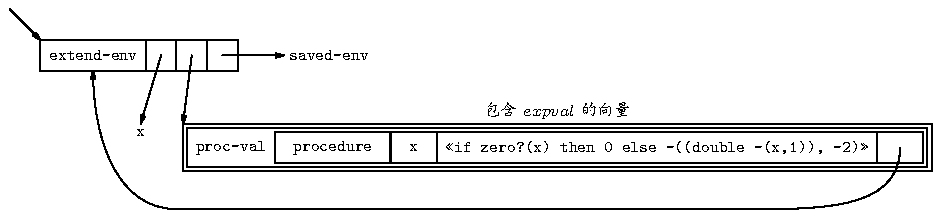
\includegraphics[scale=1.0]{vector-env.pdf}\end{SCentered}

这里是创建这种数据结构的代码:

\begin{EoplCodeInset}\begin{SCodeFlow}\begin{RktBlk}\begin{SingleColumn}\RktPn{(}\RktSym{define}\mbox{\hphantom{\Scribtexttt{x}}}\RktSym{extend{-}env{-}rec}

\mbox{\hphantom{\Scribtexttt{xx}}}\RktPn{(}\RktSym{lambda}\mbox{\hphantom{\Scribtexttt{x}}}\RktPn{(}\RktSym{p{-}names}\mbox{\hphantom{\Scribtexttt{x}}}\RktSym{b{-}vars}\mbox{\hphantom{\Scribtexttt{x}}}\RktSym{bodies}\mbox{\hphantom{\Scribtexttt{x}}}\RktSym{saved{-}env}\RktPn{)}

\mbox{\hphantom{\Scribtexttt{xxxx}}}\RktPn{(}\RktSym{let}\mbox{\hphantom{\Scribtexttt{x}}}\RktPn{(}\RktPn{(}\RktSym{vec}\mbox{\hphantom{\Scribtexttt{x}}}\RktPn{(}\RktSym{make{-}vector}\mbox{\hphantom{\Scribtexttt{x}}}\RktPn{(}\RktSym{length}\mbox{\hphantom{\Scribtexttt{x}}}\RktSym{p{-}names}\RktPn{)}\RktPn{)}\RktPn{)}\RktPn{)}

\mbox{\hphantom{\Scribtexttt{xxxxxx}}}\RktPn{(}\RktSym{let}\mbox{\hphantom{\Scribtexttt{x}}}\RktPn{(}\RktPn{(}\RktSym{new{-}env}\mbox{\hphantom{\Scribtexttt{x}}}\RktPn{(}\RktSym{extend{-}env}\mbox{\hphantom{\Scribtexttt{x}}}\RktSym{p{-}names}\mbox{\hphantom{\Scribtexttt{x}}}\RktSym{vec}\mbox{\hphantom{\Scribtexttt{x}}}\RktSym{saved{-}env}\RktPn{)}\RktPn{)}\RktPn{)}

\mbox{\hphantom{\Scribtexttt{xxxxxxxx}}}\RktPn{(}\RktSym{vector{-}set{\hbox{\texttt{!}}}}\mbox{\hphantom{\Scribtexttt{x}}}\RktSym{vec}\mbox{\hphantom{\Scribtexttt{x}}}\RktVal{0}

\mbox{\hphantom{\Scribtexttt{xxxxxxxxxx}}}\RktPn{(}\RktSym{proc{-}val}\mbox{\hphantom{\Scribtexttt{x}}}\RktPn{(}\RktSym{procedure}\mbox{\hphantom{\Scribtexttt{x}}}\RktSym{b{-}var}\mbox{\hphantom{\Scribtexttt{x}}}\RktSym{body}\mbox{\hphantom{\Scribtexttt{x}}}\RktSym{new{-}env}\RktPn{)}\RktPn{)}\RktPn{)}

\mbox{\hphantom{\Scribtexttt{xxxxxxxx}}}\RktSym{new{-}env}\RktPn{)}\RktPn{)}\RktPn{)}\RktPn{)}\end{SingleColumn}\end{RktBlk}\end{SCodeFlow}\end{EoplCodeInset}

修改环境数据类型和 \Scribtexttt{apply{-}env} 的定义,完成这种表示的实现。确保
\Scribtexttt{apply{-}env} 总是返回表达值。
\index{extendenvrec@\textbf{\Scribtexttt{extend{-}env{-}rec}}|)idxdecorator{}{}}\end{EoplExercise}

\begin{EoplExercise}\label{t:x28elem_x22ex3x2e36x22x29}\texMathInline{\textnormal{[}{\star}{\star}\textnormal{]}}\mbox{\hphantom{\Scribtexttt{x}}}\index{dzuo1guo4cheng2sheng1ming2@多过程声明|(idxdecorator{}{}}
\index{hzu4di4gui1@互递归|(idxdecorator{}{}}
\index{dzi4gui1cheng2xu4@递归程序!hzu4di4gui1@互递归|(idxdecorator{}{}}
扩展这种实现,处理ex3.32 中的语言。
\index{bzi4bao1@闭包|)idxdecorator{}{}}\end{EoplExercise}

\begin{EoplExercise}\label{t:x28elem_x22ex3x2e37x22x29}\texMathInline{\textnormal{[}{\star}{\star}\textnormal{]}}\mbox{\hphantom{\Scribtexttt{x}}}\index{dzong4tai4bang3ding4dong4tai4zuo4yong4yu4@动态绑定(动态作用域)|(idxdecorator{}{}}
\index{jzie1cheng2han2shu4@阶乘函数|(idxdecorator{}{}}
\index{dzi4gui1cheng2xu4@递归程序!szhe4ji4he2shi2xian4@设计和实现|(idxdecorator{}{}}
\index{bzian4liang4sheng1ming2dezuo4yong4yu4@变量声明的作用域!dzong4tai4@动态|(idxdecorator{}{}}
使用动态绑定(ex3.28),不需要任何特殊机制,靠 \Scribtexttt{let} 就能创建
递归过程。这是出于历史兴趣。在早年的编程语言设计中,\SecRefLocal{t:x28part_x22s3x2e4x22x29}{3.4}{LETREC:支持递归过程的语言}讨论的那些方法
还鲜为人知。要验证动态绑定实现的递归,试试程序:

\begin{EoplEquationInset}\begin{SVerbatim}\begin{SingleColumn}\Scribtexttt{let fact = proc (n) add1(n)}

\Scribtexttt{in let fact = proc (n)}

\Scribtexttt{}\mbox{\hphantom{\Scribtexttt{xxxxxxxxxxxxxxx}}}\Scribtexttt{if zero{\hbox{\texttt{?}}}(n)}

\Scribtexttt{}\mbox{\hphantom{\Scribtexttt{xxxxxxxxxxxxxxx}}}\Scribtexttt{then 1}

\Scribtexttt{}\mbox{\hphantom{\Scribtexttt{xxxxxxxxxxxxxxx}}}\Scribtexttt{else *(n, (fact {-}(n,1)))}

\Scribtexttt{}\mbox{\hphantom{\Scribtexttt{xxx}}}\Scribtexttt{in (fact 5)}\end{SingleColumn}\end{SVerbatim}\end{EoplEquationInset}

试试词法绑定,再试试动态绑定。用动态绑定的被定语言写出\SecRefLocal{t:x28part_x22s3x2e4x22x29}{3.4}{LETREC:支持递归过程的语言}中的互递归过
程 \Scribtexttt{even} 和 \Scribtexttt{odd}。
\index{dzong4tai4bang3ding4dong4tai4zuo4yong4yu4@动态绑定(动态作用域)|)idxdecorator{}{}}
\index{jzie1cheng2han2shu4@阶乘函数|)idxdecorator{}{}}
\index{dzuo1guo4cheng2sheng1ming2@多过程声明|)idxdecorator{}{}}
\index{hzu4di4gui1@互递归|)idxdecorator{}{}}
\index{dzi4gui1cheng2xu4@递归程序!szhe4ji4he2shi2xian4@设计和实现|)idxdecorator{}{}}
\index{dzi4gui1cheng2xu4@递归程序!hzu4di4gui1@互递归|)idxdecorator{}{}}
\index{bzian4liang4sheng1ming2dezuo4yong4yu4@变量声明的作用域!dzong4tai4@动态|)idxdecorator{}{}}\end{EoplExercise}

\Ssubsection{定界和变量绑定}{定界和变量绑定}\label{t:x28part_x22s3x2e5x22x29}

\index{bzang3ding4Binding@绑定 (Binding)!bzian4liang4@变量|(idxdecorator{}{}}
\index{szheng1ming2@声明!bzian4liang4@变量|(idxdecorator{}{}}
\index{yzin3yong4@引用|(idxdecorator{}{}}
\index{bzian4liang4sheng1ming2dezuo4yong4yu4@变量声明的作用域|(idxdecorator{}{}}
\index{bzian4liang4@变量!szheng1ming2@声明|(idxdecorator{}{}}
我们已经在很多地方见到过变量的声明和使用,现在我们来系统讨论这些思想。

在大多数编程语言中,变量只能以两种方式出现:\emph{引用} (\emph{reference})
或\emph{声明} (\emph{declaration})。变量引用就是使用变量。例如,在 Scheme 表达式

\begin{Subflow}\begin{EoplCodeInset}\begin{SCodeFlow}\begin{RktBlk}\begin{SingleColumn}\RktPn{(}\RktSym{f}\RktMeta{}\mbox{\hphantom{\Scribtexttt{x}}}\RktMeta{}\RktSym{x}\RktMeta{}\mbox{\hphantom{\Scribtexttt{x}}}\RktMeta{}\RktSym{y}\RktPn{)}\RktMeta{}\end{SingleColumn}\end{RktBlk}\end{SCodeFlow}\end{EoplCodeInset}

中出现的变量 \Scribtexttt{f}、\Scribtexttt{x} 和 \Scribtexttt{y} 均为引用。但在

\begin{EoplCodeInset}\begin{SCodeFlow}\begin{RktBlk}\begin{SingleColumn}\RktPn{(}\RktSym{lambda}\RktMeta{}\mbox{\hphantom{\Scribtexttt{x}}}\RktMeta{}\RktPn{(}\RktSym{x}\RktPn{)}\RktMeta{}\mbox{\hphantom{\Scribtexttt{x}}}\RktMeta{}\RktPn{(}\RktSym{+}\RktMeta{}\mbox{\hphantom{\Scribtexttt{x}}}\RktMeta{}\RktSym{x}\RktMeta{}\mbox{\hphantom{\Scribtexttt{x}}}\RktMeta{}\RktVal{3}\RktPn{)}\RktPn{)}\RktMeta{}\end{SingleColumn}\end{RktBlk}\end{SCodeFlow}\end{EoplCodeInset}

或

\begin{EoplCodeInset}\begin{SCodeFlow}\begin{RktBlk}\begin{SingleColumn}\RktPn{(}\RktSym{let}\RktMeta{}\mbox{\hphantom{\Scribtexttt{x}}}\RktMeta{}\RktPn{(}\RktPn{(}\RktSym{x}\RktMeta{}\mbox{\hphantom{\Scribtexttt{x}}}\RktMeta{}\RktPn{(}\RktSym{+}\RktMeta{}\mbox{\hphantom{\Scribtexttt{x}}}\RktMeta{}\RktSym{y}\RktMeta{}\mbox{\hphantom{\Scribtexttt{x}}}\RktMeta{}\RktVal{7}\RktPn{)}\RktPn{)}\RktPn{)}\RktMeta{}\mbox{\hphantom{\Scribtexttt{x}}}\RktMeta{}\RktPn{(}\RktSym{+}\RktMeta{}\mbox{\hphantom{\Scribtexttt{x}}}\RktMeta{}\RktSym{x}\RktMeta{}\mbox{\hphantom{\Scribtexttt{x}}}\RktMeta{}\RktVal{3}\RktPn{)}\RktPn{)}\RktMeta{}\end{SingleColumn}\end{RktBlk}\end{SCodeFlow}\end{EoplCodeInset}

中,第一个出现的 \Scribtexttt{x} 是声明:引入一个变量,作为某个值的名字。在 \Scribtexttt{lambda}
表达式中,变量的值在过程调用时提供。在 \Scribtexttt{let} 表达式中,变量的值由表达式
\Scribtexttt{(+ y z)} 求得。\end{Subflow}

我们说变量引用由对应的声明\emph{绑定} (\emph{bound}),且\emph{绑定}到它的值。
在\SecRefLocal{t:x28part_x22s1x2e2x2e4x22x29}{1.2.4}{\Scribtexttt{occurs{-}free{\hbox{\texttt{?}}}}},我们已经见过用声明绑定变量的例子。

\begin{EoplFigure}[!t]

\noindent \begin{SCentered}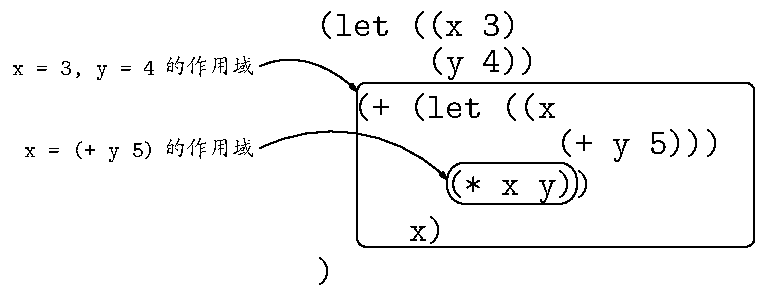
\includegraphics[scale=1.0]{simple-contour.pdf}\end{SCentered}

\caption{简单等深线\label{t:x28elem_x22figx2d3x2e13x22x29}}\end{EoplFigure}

大多数编程语言中的声明都有有限的作用域,所以同一个变量名在程序的不同部分可用于不
同的目的。例如,我们反复把 \Scribtexttt{lst} 用作绑定变量,它的作用域每次都限制在对应的
\Scribtexttt{lambda} 表达式主体内。

每种编程语言都有一些规则来判断各个变量引用指代哪一声明。这些规则通常
叫做\emph{定界} (\emph{scoping}) 规则。声明在程序中生效的部分叫做声明
的\emph{作用域} (\emph{scope})。

我们可以不加执行地判断程序中的各个变量引用对应于哪个声明。这样的性质不必执行程序
就能计算出来,名为\emph{静态} (\emph{static}) 性质。
\index{czheng2xu4dejing4tai4xing4zhi4@程序的静态性质|idxdecorator{}{}}

要找出某个变量引用对应于哪一声明,我们\emph{向外} (\emph{outward}) 查找,直到找
出变量的声明。这里是一个简单的 Scheme 示例。

\begin{EoplCodeInset}\begin{SVerbatim}\begin{SingleColumn}\Scribtexttt{(let ((x 3)}\mbox{\hphantom{\Scribtexttt{xxxxxxxxxxxxxx}}}\Scribtexttt{}\emph{称之为 \Scribtexttt{x1}}\Scribtexttt{}

\Scribtexttt{}\mbox{\hphantom{\Scribtexttt{xxxxxx}}}\Scribtexttt{(y 4))}

\Scribtexttt{}\mbox{\hphantom{\Scribtexttt{xx}}}\Scribtexttt{(+ (let ((x}\mbox{\hphantom{\Scribtexttt{xxxxxxxxxxxx}}}\Scribtexttt{}\emph{称之为 \Scribtexttt{x2}}\Scribtexttt{}

\Scribtexttt{}\mbox{\hphantom{\Scribtexttt{xxxxxxxxxxxxx}}}\Scribtexttt{(+ y 5)))}

\Scribtexttt{}\mbox{\hphantom{\Scribtexttt{xxxxxxx}}}\Scribtexttt{(* x y))}\mbox{\hphantom{\Scribtexttt{xxxxxxxxxx}}}\Scribtexttt{}\emph{这个 \Scribtexttt{x} 指代 \Scribtexttt{x2}}\Scribtexttt{}

\Scribtexttt{}\mbox{\hphantom{\Scribtexttt{xxxxx}}}\Scribtexttt{x))}\mbox{\hphantom{\Scribtexttt{xxxxxxxxxxxxxxxxx}}}\Scribtexttt{}\emph{这个 \Scribtexttt{x} 指代 \Scribtexttt{x1}}\end{SingleColumn}\end{SVerbatim}\end{EoplCodeInset}

在这个例子中,内层的 \Scribtexttt{x} 绑定到 9,所以表达式的值为

\begin{EoplCodeInset}\begin{SVerbatim}\begin{SingleColumn}\Scribtexttt{(let ((x 3)}

\Scribtexttt{}\mbox{\hphantom{\Scribtexttt{xxxxxx}}}\Scribtexttt{(y 4))}

\Scribtexttt{}\mbox{\hphantom{\Scribtexttt{xx}}}\Scribtexttt{(+ (let ((x}

\Scribtexttt{}\mbox{\hphantom{\Scribtexttt{xxxxxxxxxxxxx}}}\Scribtexttt{(+ y 5)))}

\Scribtexttt{}\mbox{\hphantom{\Scribtexttt{xxxxxxx}}}\Scribtexttt{(* x y))}

\Scribtexttt{}\mbox{\hphantom{\Scribtexttt{xxxxx}}}\Scribtexttt{x))}

\Scribtexttt{}\mbox{\hphantom{\Scribtexttt{x}}}

\Scribtexttt{= (+ (let ((x}

\Scribtexttt{}\mbox{\hphantom{\Scribtexttt{xxxxxxxxxxxxx}}}\Scribtexttt{(+ 4 5)))}

\Scribtexttt{}\mbox{\hphantom{\Scribtexttt{xxxxxxx}}}\Scribtexttt{(* x 4))}

\Scribtexttt{}\mbox{\hphantom{\Scribtexttt{xxxxx}}}\Scribtexttt{3)}

\Scribtexttt{}\mbox{\hphantom{\Scribtexttt{x}}}

\Scribtexttt{= (+ (let ((x 9))}

\Scribtexttt{}\mbox{\hphantom{\Scribtexttt{xxxxxxx}}}\Scribtexttt{(* x 4))}

\Scribtexttt{}\mbox{\hphantom{\Scribtexttt{xxxxx}}}\Scribtexttt{3)}

\Scribtexttt{}\mbox{\hphantom{\Scribtexttt{x}}}

\Scribtexttt{= (+ 36}

\Scribtexttt{}\mbox{\hphantom{\Scribtexttt{xxxxx}}}\Scribtexttt{3)}

\Scribtexttt{}\mbox{\hphantom{\Scribtexttt{x}}}

\Scribtexttt{= 39}\end{SingleColumn}\end{SVerbatim}\end{EoplCodeInset}

\index{czi2fa3zuo4yong4yu4gui1ze2@词法作用域规则|idxdecorator{}{}}
这样的定界规则叫做\emph{词法定界} (\emph{lexical scoping}) 规则,这样声明的变量
叫做\emph{词法变量} (\emph{lexical variable})。
\index{czi2fa3bian4liang4@词法变量|idxdecorator{}{}}
\index{bzian4liang4@变量!czi2fa3@词法|idxdecorator{}{}}

使用词法定界,我们可以重新声明一个变量,给作用域戳个“洞
”。这样的内层声明\emph{遮蔽} (\emph{shadow}) \index{zzhe1bi4@遮蔽|idxdecorator{}{}}
\index{bzian4liang4@变量!zzhe1bi4@遮蔽|idxdecorator{}{}}
外层声明。 例如,在上例的乘式 \Scribtexttt{(* x y)} 中,内层的 \Scribtexttt{x} 遮蔽了外层的。

\index{dzeng3shen1xian4@等深线|idxdecorator{}{}}
词法作用域是嵌套式的:每个作用域完全包裹在另一个里面。我们用\emph{等深线} (\emph{contour
diagram}) 解释这点。 展示了上例的等深线。每个作用域
用一个框圈起来,箭头连接声明与其作用域。

 展示了一个更复杂的程序和它的等深线。其中的第 5 行、第 7 行
和第 8 行,表达式 \Scribtexttt{(+ x y z)} 出现了三次。第 5 行在 \Scribtexttt{x2} 和 \Scribtexttt{z2} 的作用
域内,\Scribtexttt{x2} 和 \Scribtexttt{z2} 的作用域在 \Scribtexttt{z1} 的作用域内,\Scribtexttt{z1} 的作用域在
\Scribtexttt{x1} 和 \Scribtexttt{y1} 的作用域内。所以,第5行的 \Scribtexttt{x} 指代 \Scribtexttt{x2},\Scribtexttt{y} 指代
\Scribtexttt{y1},\Scribtexttt{z} 指代 \Scribtexttt{z2}。第 7 行在 \Scribtexttt{x4} 和 \Scribtexttt{y2} 的作用域内,\Scribtexttt{x4}
和\Scribtexttt{y2} 的作用域在 \Scribtexttt{x2} 和 \Scribtexttt{z2} 的作用域内,\Scribtexttt{x2} 和 \Scribtexttt{z2} 的作用域
在\Scribtexttt{z1} 的作用域内,\Scribtexttt{z1} 的作用域在 \Scribtexttt{x1} 和 \Scribtexttt{y1} 的作用域内。所以,第
7行的 \Scribtexttt{x} 指代 \Scribtexttt{x4},\Scribtexttt{y} 指代 \Scribtexttt{y2},\Scribtexttt{z} 指代 \Scribtexttt{z2}。最后,第 8
行在 \Scribtexttt{x3} 的作用域内,\Scribtexttt{x3} 的作用域在 \Scribtexttt{x2} 和 \Scribtexttt{z2} 的作用域内,
\Scribtexttt{x2} 和 \Scribtexttt{z2} 的作用域在 \Scribtexttt{z1} 的作用域内,\Scribtexttt{z1} 的作用域在 \Scribtexttt{x1} 和
\Scribtexttt{y1} 的作用域内。所以,第8行的 \Scribtexttt{x} 指代 \Scribtexttt{x3},\Scribtexttt{y} 指代 \Scribtexttt{y1},
\Scribtexttt{z} 指代\Scribtexttt{z2}。

\begin{EoplFigure}\begin{SCentered}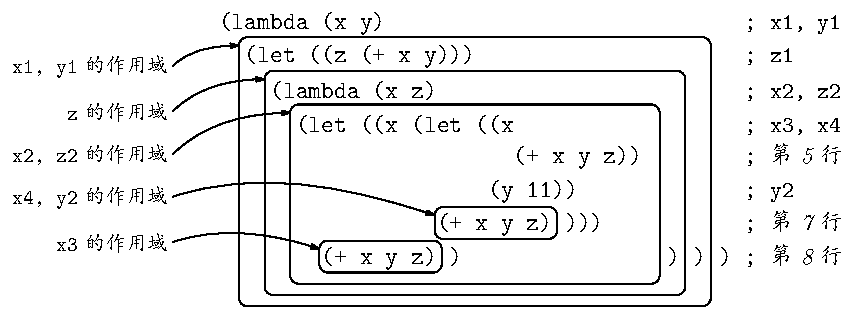
\includegraphics[scale=1.0]{complicated-contour.pdf}\end{SCentered}

\caption{较复杂的等深线\label{t:x28elem_x22figx2d3x2e14x22x29}}\end{EoplFigure}

变量与值的对应关系叫做\emph{绑定} (\emph{binding})。我们可以通过规范来理解如何创
建绑定。

\index{bzang3ding4Binding@绑定 (Binding)!proc@\Scribtexttt{proc}|idxdecorator{}{}}
\index{zzhu3ti3@主体!proc@\Scribtexttt{proc}|idxdecorator{}{}}
由 \Scribtexttt{proc} 声明的变量在过程调用时绑定。

\begin{EoplEquationInset}\begin{SVerbatim}\begin{SingleColumn}\Scribtexttt{(apply{-}procedure (procedure }\texMathInline{var}\Scribtexttt{}\mbox{\hphantom{\Scribtexttt{x}}}\Scribtexttt{}\texMathInline{body}\Scribtexttt{}\mbox{\hphantom{\Scribtexttt{x}}}\Scribtexttt{}\texMathInline{\rho}\Scribtexttt{) }\texMathInline{val}\Scribtexttt{)}

\Scribtexttt{= (value{-}of }\texMathInline{body}\Scribtexttt{}\mbox{\hphantom{\Scribtexttt{x}}}\Scribtexttt{(extend{-}env }\texMathInline{var}\Scribtexttt{}\mbox{\hphantom{\Scribtexttt{x}}}\Scribtexttt{}\texMathInline{val}\Scribtexttt{}\mbox{\hphantom{\Scribtexttt{x}}}\Scribtexttt{}\texMathInline{\rho}\Scribtexttt{))}\end{SingleColumn}\end{SVerbatim}\end{EoplEquationInset}

\index{bzang3ding4Binding@绑定 (Binding)!let@\Scribtexttt{let}|idxdecorator{}{}}
\index{zzhu3ti3@主体!let@\Scribtexttt{let}|idxdecorator{}{}}
\Scribtexttt{let} 声明的变量绑定到声明右边的值。

\begin{EoplEquationInset}\begin{SVerbatim}\begin{SingleColumn}\Scribtexttt{(value{-}of (let{-}exp }\texMathInline{var}\Scribtexttt{}\mbox{\hphantom{\Scribtexttt{x}}}\Scribtexttt{}\texMathInline{val}\Scribtexttt{}\mbox{\hphantom{\Scribtexttt{x}}}\Scribtexttt{}\texMathInline{body}\Scribtexttt{) }\texMathInline{\rho}\Scribtexttt{)}

\Scribtexttt{= (value{-}of }\texMathInline{body}\Scribtexttt{}\mbox{\hphantom{\Scribtexttt{x}}}\Scribtexttt{(extend{-}env }\texMathInline{var}\Scribtexttt{}\mbox{\hphantom{\Scribtexttt{x}}}\Scribtexttt{}\texMathInline{val}\Scribtexttt{}\mbox{\hphantom{\Scribtexttt{x}}}\Scribtexttt{}\texMathInline{\rho}\Scribtexttt{))}\end{SingleColumn}\end{SVerbatim}\end{EoplEquationInset}

\index{bzang3ding4Binding@绑定 (Binding)!letrec@\Scribtexttt{letrec}|idxdecorator{}{}}
\index{zzhu3ti3@主体!letrec@\Scribtexttt{letrec}|idxdecorator{}{}}
\Scribtexttt{letrec} 声明的变量也要绑定到声明右边的值。

\begin{EoplEquationInset}\begin{SVerbatim}\begin{SingleColumn}\Scribtexttt{(value{-}of}

\Scribtexttt{}\mbox{\hphantom{\Scribtexttt{xx}}}\Scribtexttt{(letrec{-}exp }\texMathInline{proc\mbox{-}name}\Scribtexttt{}\mbox{\hphantom{\Scribtexttt{x}}}\Scribtexttt{}\texMathInline{bound\mbox{-}var}\Scribtexttt{}\mbox{\hphantom{\Scribtexttt{x}}}\Scribtexttt{}\texMathInline{proc\mbox{-}body}\Scribtexttt{}\mbox{\hphantom{\Scribtexttt{x}}}\Scribtexttt{}\texMathInline{letrec\mbox{-}body}\Scribtexttt{)}

\Scribtexttt{}\mbox{\hphantom{\Scribtexttt{xx}}}\Scribtexttt{}\texMathInline{\rho}\Scribtexttt{)}

\Scribtexttt{= (value{-}of}

\Scribtexttt{}\mbox{\hphantom{\Scribtexttt{xxxx}}}\Scribtexttt{}\texMathInline{letrec\mbox{-}body}\Scribtexttt{}

\Scribtexttt{}\mbox{\hphantom{\Scribtexttt{xxxx}}}\Scribtexttt{(extend{-}env{-}rec }\texMathInline{proc\mbox{-}name}\Scribtexttt{}\mbox{\hphantom{\Scribtexttt{x}}}\Scribtexttt{}\texMathInline{bound\mbox{-}var}\Scribtexttt{}\mbox{\hphantom{\Scribtexttt{x}}}\Scribtexttt{}\texMathInline{proc\mbox{-}body}\Scribtexttt{}\mbox{\hphantom{\Scribtexttt{x}}}\Scribtexttt{}\texMathInline{\rho}\Scribtexttt{))}\end{SingleColumn}\end{SVerbatim}\end{EoplEquationInset}

\index{bzang3ding4Binding@绑定 (Binding)!qzi1xian4@期限|idxdecorator{}{}}
\index{czheng2xu4dedong4tai4xing4zhi4@程序的动态性质|(idxdecorator{}{}}
\index{bzian4liang4bang3ding4deqi1xian4@变量绑定的期限|idxdecorator{}{}}
\index{bzan4wu2xian4deqi1xian4@半无限的期限|idxdecorator{}{}}
\index{bzian4liang4@变量!qzi1xian4@期限|idxdecorator{}{}}
绑定的\emph{期限} (\emph{extent}) 指绑定保持的时长。在我们的语言中,就像在
Scheme 中一样,所有的绑定都是\emph{半无限} (\emph{semi{-}infinite}) 的,意思是变量
一旦绑定,该绑定就要(至少是有可能)无限期地保留。这是因为绑定可能隐藏在已返回的
闭包之中。在半无限的语言中,垃圾回收器收集不能再访问的绑定。这只能在运行时判定,
因此我们说这是一条\emph{动态} (\emph{dynamic}) 性质。

很可惜的是,“动态”有时表示“在表达式求
值期间”,有时又表示“无法事先计算”。如
果我们不允许 \Scribtexttt{let} 的值为过程,那么 let 绑定会在 \Scribtexttt{let} 主体求值结束时到期。
这叫做\emph{动态}期限,而它是一条\emph{静态}性质。
\index{czheng2xu4dejing4tai4xing4zhi4@程序的静态性质|idxdecorator{}{}}
因为这种期限是一条静态性质,所以我们可以准确预测绑定何时可以抛弃。
ex3.28 等几道练习中的动态绑定表现类似。
\index{bzang3ding4Binding@绑定 (Binding)!bzian4liang4@变量|)idxdecorator{}{}}
\index{szheng1ming2@声明!bzian4liang4@变量|)idxdecorator{}{}}
\index{czheng2xu4dedong4tai4xing4zhi4@程序的动态性质|)idxdecorator{}{}}
\index{yzin3yong4@引用|)idxdecorator{}{}}
\index{bzian4liang4sheng1ming2dezuo4yong4yu4@变量声明的作用域|)idxdecorator{}{}}
\index{bzian4liang4@变量!szheng1ming2@声明|)idxdecorator{}{}}

\Ssubsection{消除变量名}{消除变量名}\label{t:x28part_x22s3x2e6x22x29}

\index{dze2bu4lu3jin1suo3yin3@德布鲁金索引|(idxdecorator{}{}}
\index{LETREC!wzu2ming2ban3ben3@无名版本|(idxdecorator{}{}}
\index{czi2fa3xun2zhi3@词法寻址|(idxdecorator{}{}}
\index{qzu4ming2@去名!LETREC@LETREC|(idxdecorator{}{}}
\index{bzian4liang4@变量!szheng1ming2@声明|(idxdecorator{}{}}
定界算法的执行过程可以看作始自变量引用的外出旅行。在旅途中,到达对应的声明之前可
能会跨越多条等深线。跨越的等深线数目叫做变量引用的\emph{词深} (\emph{lexical
depth})(或\emph{静深} (\emph{static depth}))。由于惯用“从0开始的
索引”,所以不计最后跨过的等深线。例如,在 Scheme 表达式

\begin{Subflow}\begin{EoplCodeInset}\begin{SCodeFlow}\begin{RktBlk}\begin{SingleColumn}\RktPn{(}\RktSym{lambda}\mbox{\hphantom{\Scribtexttt{x}}}\RktPn{(}\RktSym{x}\RktPn{)}

\mbox{\hphantom{\Scribtexttt{xx}}}\RktPn{(}\RktPn{(}\RktSym{lambda}\mbox{\hphantom{\Scribtexttt{x}}}\RktPn{(}\RktSym{a}\RktPn{)}

\mbox{\hphantom{\Scribtexttt{xxxxx}}}\RktPn{(}\RktSym{x}\mbox{\hphantom{\Scribtexttt{x}}}\RktSym{a}\RktPn{)}\RktPn{)}

\mbox{\hphantom{\Scribtexttt{xxx}}}\RktSym{x}\RktPn{)}\RktPn{)}\end{SingleColumn}\end{RktBlk}\end{SCodeFlow}\end{EoplCodeInset}

中,最后一行 \Scribtexttt{x} 的引用以及 \Scribtexttt{a} 的引用词深均为 0,而第三行 \Scribtexttt{x} 的引用词
深为 1。\end{Subflow}

因此,我们可以完全消除变量名,写成这样

\begin{Subflow}\begin{EoplCodeInset}\begin{SVerbatim}\begin{SingleColumn}\Scribtexttt{(nameless{-}lambda}

\Scribtexttt{}\mbox{\hphantom{\Scribtexttt{xx}}}\Scribtexttt{((nameless{-}lambda}

\Scribtexttt{}\mbox{\hphantom{\Scribtexttt{xxxxx}}}\Scribtexttt{(\#1 \#0))}

\Scribtexttt{}\mbox{\hphantom{\Scribtexttt{xxx}}}\Scribtexttt{\#0))}\end{SingleColumn}\end{SVerbatim}\end{EoplCodeInset}

这里,每个 \Scribtexttt{nameless{-}lambda} 都声明了一个新的无名变量,每个变量引用由其词深替
代;这个数字准确标示了要使用的声明。这些数字叫做\emph{词法地址} (\emph{lexical
address}) 或\emph{德布鲁金索引} (\emph{de Bruijn index})。编译器例行计算每个变量
引用的词法地址。除非用来提供调试信息,计算一旦完成,变量名即可丢弃。\end{Subflow}

这样记录信息有用,因为词法地址\emph{预测}了怎样从环境中找出某个变量。

考虑我们语言中的表达式

\begin{Subflow}\begin{EoplCodeInset}\begin{SVerbatim}\begin{SingleColumn}\Scribtexttt{let x = }\texMathInline{exp_1}\Scribtexttt{}

\Scribtexttt{in let y = }\texMathInline{exp_2}\Scribtexttt{}

\Scribtexttt{}\mbox{\hphantom{\Scribtexttt{xxx}}}\Scribtexttt{in {-}(x,y)}\end{SingleColumn}\end{SVerbatim}\end{EoplCodeInset}

在差值表达式中,\Scribtexttt{y} 和 \Scribtexttt{x} 的词深分别为0和1。\end{Subflow}

现在假设在某个适当环境中求得 \texMathInline{exp_1} 和 \texMathInline{exp_2} 的值,分别为 \texMathInline{val_1} 和
\texMathInline{val_2},那么这个表达式的值为

\begin{Subflow}\begin{EoplEquationInset}\begin{SVerbatim}\begin{SingleColumn}\Scribtexttt{(value{-}of}

\Scribtexttt{}\mbox{\hphantom{\Scribtexttt{xx}}}\Scribtexttt{{\Stttextless}{\Stttextless}let x = }\texMathInline{exp_1}\Scribtexttt{}

\Scribtexttt{}\mbox{\hphantom{\Scribtexttt{xxxx}}}\Scribtexttt{in let y = }\texMathInline{exp_2}\Scribtexttt{}

\Scribtexttt{}\mbox{\hphantom{\Scribtexttt{xxxxxxx}}}\Scribtexttt{in {-}(x,y){\Stttextmore}{\Stttextmore}}

\Scribtexttt{}\mbox{\hphantom{\Scribtexttt{xx}}}\Scribtexttt{}\texMathInline{\rho}\Scribtexttt{)}

\Scribtexttt{=}

\Scribtexttt{(value{-}of}

\Scribtexttt{}\mbox{\hphantom{\Scribtexttt{xx}}}\Scribtexttt{{\Stttextless}{\Stttextless}let y = }\texMathInline{exp_2}\Scribtexttt{}

\Scribtexttt{}\mbox{\hphantom{\Scribtexttt{xxxx}}}\Scribtexttt{in {-}(x,y){\Stttextmore}{\Stttextmore}}

\Scribtexttt{}\mbox{\hphantom{\Scribtexttt{xx}}}\Scribtexttt{[x=}\texMathInline{val_1}\Scribtexttt{]}\texMathInline{\rho}\Scribtexttt{)}

\Scribtexttt{=}

\Scribtexttt{(value{-}of}

\Scribtexttt{}\mbox{\hphantom{\Scribtexttt{xx}}}\Scribtexttt{{\Stttextless}{\Stttextless}{-}(x,y){\Stttextmore}{\Stttextmore}}

\Scribtexttt{}\mbox{\hphantom{\Scribtexttt{xx}}}\Scribtexttt{[y=}\texMathInline{val_2}\Scribtexttt{][x=}\texMathInline{val_1}\Scribtexttt{]}\texMathInline{\rho}\Scribtexttt{)}\end{SingleColumn}\end{SVerbatim}\end{EoplEquationInset}

所以,求差值表达式的值时,\Scribtexttt{y} 深度为 0,\Scribtexttt{x} 深度为 1,正如词深预测的那样。\end{Subflow}

如果用关联列表表示环境(见ex2.5),那么环境看起来像是

\begin{Subflow}\begin{SCentered}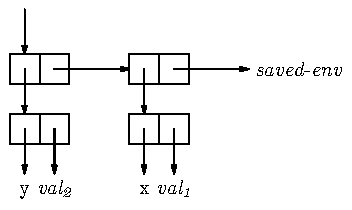
\includegraphics[scale=1.0]{lexical-addr-env.pdf}\end{SCentered}

所以不论 \texMathInline{val_1} 和 \texMathInline{val_2} 值为何,\Scribtexttt{x} 和 \Scribtexttt{y} 的值都是取环境中第 1 个
元素的余项和第 0 个元素的余项。\end{Subflow}

过程的主体也是这样。考虑

\begin{Subflow}\begin{EoplCodeInset}\begin{SVerbatim}\begin{SingleColumn}\Scribtexttt{let a = 5}

\Scribtexttt{in proc (x) {-}(x,1)}\end{SingleColumn}\end{SVerbatim}\end{EoplCodeInset}

在过程的主体中,\Scribtexttt{x} 的词深是 0,\Scribtexttt{a} 的词深是 1。\end{Subflow}

这个表达式的值为:

\begin{EoplEquationInset}\begin{SVerbatim}\begin{SingleColumn}\Scribtexttt{(value{-}of}

\Scribtexttt{}\mbox{\hphantom{\Scribtexttt{xx}}}\Scribtexttt{{\Stttextless}{\Stttextless}let a = 5 in proc (x) {-}(x,a){\Stttextmore}{\Stttextmore}}

\Scribtexttt{}\mbox{\hphantom{\Scribtexttt{xx}}}\Scribtexttt{}\texMathInline{\rho}\Scribtexttt{)}

\Scribtexttt{= (value{-}of {\Stttextless}{\Stttextless}proc (x) {-}(x,a){\Stttextmore}{\Stttextmore}}

\Scribtexttt{}\mbox{\hphantom{\Scribtexttt{xxxx}}}\Scribtexttt{(extend{-}env a }\texMathInline{\lceil}\Scribtexttt{5}\texMathInline{\rceil}\Scribtexttt{}\mbox{\hphantom{\Scribtexttt{x}}}\Scribtexttt{}\texMathInline{\rho}\Scribtexttt{))}

\Scribtexttt{= (proc{-}val (procedure x {\Stttextless}{\Stttextless}{-}(x,a){\Stttextmore}{\Stttextmore} [a=}\texMathInline{\lceil}\Scribtexttt{5}\texMathInline{\rceil}\Scribtexttt{]}\texMathInline{\rho}\Scribtexttt{))}\end{SingleColumn}\end{SVerbatim}\end{EoplEquationInset}

这个过程的主体只能通过 \Scribtexttt{apply{-}procedure} 求值:

\begin{EoplEquationInset}\begin{SVerbatim}\begin{SingleColumn}\Scribtexttt{(apply{-}procedure}

\Scribtexttt{}\mbox{\hphantom{\Scribtexttt{xx}}}\Scribtexttt{(procedure x {\Stttextless}{\Stttextless}{-}(x,a){\Stttextmore}{\Stttextmore} [a=}\texMathInline{\lceil}\Scribtexttt{5}\texMathInline{\rceil}\Scribtexttt{]}\texMathInline{\rho}\Scribtexttt{)}

\Scribtexttt{}\mbox{\hphantom{\Scribtexttt{xx}}}\Scribtexttt{}\texMathInline{\lceil}\Scribtexttt{7}\texMathInline{\rceil}\Scribtexttt{)}

\Scribtexttt{= (value{-}of {\Stttextless}{\Stttextless}{-}(x,a){\Stttextmore}{\Stttextmore}}

\Scribtexttt{}\mbox{\hphantom{\Scribtexttt{xxxx}}}\Scribtexttt{[x=}\texMathInline{\lceil}\Scribtexttt{7}\texMathInline{\rceil}\Scribtexttt{][a=}\texMathInline{\lceil}\Scribtexttt{5}\texMathInline{\rceil}\Scribtexttt{]}\texMathInline{\rho}\Scribtexttt{)}\end{SingleColumn}\end{SVerbatim}\end{EoplEquationInset}

每个变量又一次出现在词深预测的环境位置。
\index{dze2bu4lu3jin1suo3yin3@德布鲁金索引|)idxdecorator{}{}}
\index{czi2fa3xun2zhi3@词法寻址|)idxdecorator{}{}}

\Ssubsection{实现词法地址}{实现词法地址}\label{t:x28part_x22s3x2e7x22x29}

\index{fzan1yi4@翻译!yzou3ming2dao4wu2ming2LETREC@有名到无名 LETREC|(idxdecorator{}{}}
现在,我们来实现上述词法地址分析。我们写出过程 \Scribtexttt{translation{-}of{-}program},它取
一程序,从声明中移除所有变量,并将每个变量引用替换为词深。

例如,程序

\begin{Subflow}\begin{EoplCodeInset}\begin{SVerbatim}\begin{SingleColumn}\label{t:x28elem_x22s3x2e7x2degx22x29}\Scribtexttt{let x = 37}

\Scribtexttt{in proc (y)}

\Scribtexttt{}\mbox{\hphantom{\Scribtexttt{xxxx}}}\Scribtexttt{let z = {-}(y,x)}

\Scribtexttt{}\mbox{\hphantom{\Scribtexttt{xxxx}}}\Scribtexttt{in {-}(x,y)}\end{SingleColumn}\end{SVerbatim}\end{EoplCodeInset}

将翻译为

\begin{EoplCodeInset}\begin{SCodeFlow}\begin{RktBlk}\begin{SingleColumn}\RktVal{\#}\RktVal{(}\RktVal{struct{\hbox{\texttt{:}}}a{-}program}

\mbox{\hphantom{\Scribtexttt{xxx}}}\RktVal{\#}\RktVal{(}\RktVal{struct{\hbox{\texttt{:}}}nameless{-}let{-}exp}

\mbox{\hphantom{\Scribtexttt{xxxxxx}}}\RktVal{\#}\RktVal{(}\RktVal{struct{\hbox{\texttt{:}}}const{-}exp}\mbox{\hphantom{\Scribtexttt{x}}}\RktVal{37}\RktVal{)}

\mbox{\hphantom{\Scribtexttt{xxxxxx}}}\RktVal{\#}\RktVal{(}\RktVal{struct{\hbox{\texttt{:}}}nameless{-}proc{-}exp}

\mbox{\hphantom{\Scribtexttt{xxxxxxxxx}}}\RktVal{\#}\RktVal{(}\RktVal{struct{\hbox{\texttt{:}}}nameless{-}let{-}exp}

\mbox{\hphantom{\Scribtexttt{xxxxxxxxxxxx}}}\RktVal{\#}\RktVal{(}\RktVal{struct{\hbox{\texttt{:}}}diff{-}exp}

\mbox{\hphantom{\Scribtexttt{xxxxxxxxxxxxxxx}}}\RktVal{\#}\RktVal{(}\RktVal{struct{\hbox{\texttt{:}}}nameless{-}var{-}exp}\mbox{\hphantom{\Scribtexttt{x}}}\RktVal{0}\RktVal{)}

\mbox{\hphantom{\Scribtexttt{xxxxxxxxxxxxxxx}}}\RktVal{\#}\RktVal{(}\RktVal{struct{\hbox{\texttt{:}}}nameless{-}var{-}exp}\mbox{\hphantom{\Scribtexttt{x}}}\RktVal{1}\RktVal{)}\RktVal{)}

\mbox{\hphantom{\Scribtexttt{xxxxxxxxxxxx}}}\RktVal{\#}\RktVal{(}\RktVal{struct{\hbox{\texttt{:}}}diff{-}exp}

\mbox{\hphantom{\Scribtexttt{xxxxxxxxxxxxxxx}}}\RktVal{\#}\RktVal{(}\RktVal{struct{\hbox{\texttt{:}}}nameless{-}var{-}exp}\mbox{\hphantom{\Scribtexttt{x}}}\RktVal{2}\RktVal{)}

\mbox{\hphantom{\Scribtexttt{xxxxxxxxxxxxxxx}}}\RktVal{\#}\RktVal{(}\RktVal{struct{\hbox{\texttt{:}}}nameless{-}var{-}exp}\mbox{\hphantom{\Scribtexttt{x}}}\RktVal{1}\RktVal{)}\RktVal{)}\RktVal{)}\RktVal{)}\RktVal{)}\RktVal{)}\end{SingleColumn}\end{RktBlk}\end{SCodeFlow}\end{EoplCodeInset}

然后,我们写出新版的 \Scribtexttt{value{-}of{-}program} 来求无名程序的值,它不需要把变量放入
环境中。\end{Subflow}

\Ssubsubsection{翻译器}{翻译器}\label{t:x28part_x22s3x2e7x2e1x22x29}

因为是写翻译器,我们得知道源语言和目标语言。目标语言中的某些部分源语言中没有,例
如 \Scribtexttt{nameless{-}var{-}exp} 和 \Scribtexttt{nameless{-}let{-}exp};源语言中的某些部分目标语言中
没有,它们由后者中的对应结构取代,例如 \Scribtexttt{var{-}exp} 和 \Scribtexttt{let{-}exp}。

我们可以为每种语言写一个 \Scribtexttt{define{-}datatype},也可以让二者共用一个。因为我们使
用的前端是 SLLGEN,后者更容易。我们给 SLLGEN 的语法添加生成式:

\Iidentity{\begin{align*}\mathit{Expression} &::= \Scribtexttt{\%lexref }\Iidentity{\mathit{number}} \\[-3pt]
  &\mathrel{\phantom{::=}} \fbox{\Scribtexttt{nameless{-}var{-}exp (num)}} \\[5pt]
\mathit{Expression} &::= \Scribtexttt{\%let }\Iidentity{\mathit{Expression}}\Scribtexttt{ in }\Iidentity{\mathit{Expression}} \\[-3pt]
  &\mathrel{\phantom{::=}} \fbox{\Scribtexttt{nameless{-}let{-}exp (exp1 body)}} \\[5pt]
\mathit{Expression} &::= \Scribtexttt{\%lexproc }\Iidentity{\mathit{Expression}} \\[-3pt]
  &\mathrel{\phantom{::=}} \fbox{\Scribtexttt{nameless{-}proc{-}exp (body)}}\end{align*}}

新的构造器名字用 \Scribtexttt{\%} 开头,因为在我们的语言中,\Scribtexttt{\%} 通常是注释字符。

我们的翻译器将拒绝任何含有无名结构(\Scribtexttt{nameless{-}var{-}exp}、\Scribtexttt{nameless{-}let{-}exp}
或 \Scribtexttt{nameless{-}proc{-}exp})的程序。我们的解释器将拒绝任何含有原先具名结构
(\Scribtexttt{var{-}exp}、\Scribtexttt{let{-}exp} 或 \Scribtexttt{proc{-}exp})的程序,因为它们理应被替换。

要计算任何变量引用的词法地址,我们需要它所在的作用域。这是一种\emph{上下文} (\emph{context}) 信息,所以它和\SecRefLocal{t:x28part_x22s1x2e3x22x29}{1.3}{辅助过程和上下文参数}的继承属性类似。

\index{hzuan2jing4@环境!jzing4tai4@静态|(idxdecorator{}{}}
\index{jzing4tai4huan2jing4@静态环境|(idxdecorator{}{}}
所以 \Scribtexttt{translation{-}of{-}program} 将取两个参数:一个表达式和一个\emph{静态环境} (\emph{static
environment})。静态环境是一个变量列表,表示当前表达式所在的作用域。最
内部作用域声明的变量成为列表的第一个元素。

例如,翻译上例中的最后一行时,静态环境为:

\begin{Subflow}\begin{SCentered}\Scribtexttt{(z y x)}\end{SCentered}

所以,在静态环境中搜索变量就是查找它在静态环境中的位置,也就是词法地址:查得
\Scribtexttt{x} 为 2,\Scribtexttt{y} 为 1,\Scribtexttt{z} 为 0。\end{Subflow}

\begin{EoplFigure}[!t]


\begin{SCodeFlow}\begin{RktBlk}\begin{SingleColumn}\texMathInline{\mathit{Senv}} = \texMathInline{\mathit{Listof}}\Scribtexttt{(}\texMathInline{\mathit{Sym}}\Scribtexttt{)}

\texMathInline{\mathit{Lexaddr}} = \texMathInline{\mathit{N}}

\mbox{\hphantom{\Scribtexttt{x}}}

\textbf{\Scribtexttt{empty{-}senv}} : \texMathInline{\mathit{()} \to \mathit{Senv}}

\RktPn{(}\RktSym{define}\mbox{\hphantom{\Scribtexttt{x}}}\RktSym{empty{-}senv}

\mbox{\hphantom{\Scribtexttt{xx}}}\RktPn{(}\RktSym{lambda}\mbox{\hphantom{\Scribtexttt{x}}}\RktPn{(}\RktPn{)}

\mbox{\hphantom{\Scribtexttt{xxxx}}}\RktVal{{\textquotesingle}}\RktVal{(}\RktVal{)}\RktPn{)}\RktPn{)}

\mbox{\hphantom{\Scribtexttt{x}}}

\textbf{\Scribtexttt{extend{-}senv}} : \texMathInline{\mathit{Var} \times \mathit{Senv} \to \mathit{Senv}}

\RktPn{(}\RktSym{define}\mbox{\hphantom{\Scribtexttt{x}}}\RktSym{extend{-}senv}

\mbox{\hphantom{\Scribtexttt{xx}}}\RktPn{(}\RktSym{lambda}\mbox{\hphantom{\Scribtexttt{x}}}\RktPn{(}\RktSym{var}\mbox{\hphantom{\Scribtexttt{x}}}\RktSym{senv}\RktPn{)}

\mbox{\hphantom{\Scribtexttt{xxxx}}}\RktPn{(}\RktSym{cons}\mbox{\hphantom{\Scribtexttt{x}}}\RktSym{var}\mbox{\hphantom{\Scribtexttt{x}}}\RktSym{senv}\RktPn{)}\RktPn{)}\RktPn{)}

\mbox{\hphantom{\Scribtexttt{x}}}

\textbf{\Scribtexttt{apply{-}senv}} : \texMathInline{\mathit{Senv} \times \mathit{Var} \to \mathit{Lexaddr}}

\RktPn{(}\RktSym{define}\mbox{\hphantom{\Scribtexttt{x}}}\RktSym{apply{-}senv}

\mbox{\hphantom{\Scribtexttt{xx}}}\RktPn{(}\RktSym{lambda}\mbox{\hphantom{\Scribtexttt{x}}}\RktPn{(}\RktSym{senv}\mbox{\hphantom{\Scribtexttt{x}}}\RktSym{var}\RktPn{)}

\mbox{\hphantom{\Scribtexttt{xxxx}}}\RktPn{(}\RktSym{cond}

\mbox{\hphantom{\Scribtexttt{xxxxxx}}}\RktPn{(}\RktPn{(}\RktSym{null{\hbox{\texttt{?}}}}\mbox{\hphantom{\Scribtexttt{x}}}\RktSym{senv}\RktPn{)}

\mbox{\hphantom{\Scribtexttt{xxxxxxx}}}\RktPn{(}\RktSym{report{-}no{-}binding{-}found}\mbox{\hphantom{\Scribtexttt{x}}}\RktSym{var}\RktPn{)}\RktPn{)}

\mbox{\hphantom{\Scribtexttt{xxxxxx}}}\RktPn{(}\RktPn{(}\RktSym{eqv{\hbox{\texttt{?}}}}\mbox{\hphantom{\Scribtexttt{x}}}\RktSym{var}\mbox{\hphantom{\Scribtexttt{x}}}\RktPn{(}\RktSym{car}\mbox{\hphantom{\Scribtexttt{x}}}\RktSym{senv}\RktPn{)}\RktPn{)}

\mbox{\hphantom{\Scribtexttt{xxxxxxx}}}\RktVal{0}\RktPn{)}

\mbox{\hphantom{\Scribtexttt{xxxxxx}}}\RktPn{(}\RktSym{else}

\mbox{\hphantom{\Scribtexttt{xxxxxxxx}}}\RktPn{(}\RktSym{+}\mbox{\hphantom{\Scribtexttt{x}}}\RktVal{1}\mbox{\hphantom{\Scribtexttt{x}}}\RktPn{(}\RktSym{apply{-}senv}\mbox{\hphantom{\Scribtexttt{x}}}\RktPn{(}\RktSym{cdr}\mbox{\hphantom{\Scribtexttt{x}}}\RktSym{senv}\RktPn{)}\mbox{\hphantom{\Scribtexttt{x}}}\RktSym{var}\RktPn{)}\RktPn{)}\RktPn{)}\RktPn{)}\RktPn{)}\RktPn{)}\end{SingleColumn}\end{RktBlk}\end{SCodeFlow}

\caption{实现静态环境\label{t:x28elem_x22figx2d3x2e15x22x29}}\end{EoplFigure}

进入新的作用域就要给静态环境添加一个新元素。我们添加过程 \Scribtexttt{extend{-}senv} 来完成
这一步。

由于静态环境只是变量列表,这些过程很容易实现,如 所示。

翻译器有两个过程:\Scribtexttt{translation{-}of} 处理表达式,\Scribtexttt{translation{-}of{-}program} 处
理程序。

\Scribtexttt{senv} 表示一些声明,我们从中翻译表达式 \Scribtexttt{e}。要完成这点,我们像ex1.33 或
ex2.26 那样递归复制语法树,除了\hspace*{\fill}\\

\begin{Subflow}\begin{enumerate}\atItemizeStart

\item 调用 \Scribtexttt{apply{-}senv},用正确的词法地址,把每个 \Scribtexttt{var{-}exp} 替换为
\Scribtexttt{nameless{-}var{-}exp}。

\item 把每个 \Scribtexttt{let{-}exp} 替换为一个 \Scribtexttt{nameless{-}let{-}exp}。新表达式的右侧由旧
表达式的右侧译得。它与原式的作用域相同,所以我们在同样的静态环境 \Scribtexttt{senv} 中翻
译它。新表达式的主体由旧表达式的主体译得。但是主体位于新的作用域内,多了一个绑
定变量 \texMathInline{var}。所以我们在静态环境 \Scribtexttt{(extend{-}senv }\texMathInline{var}\Scribtexttt{ }\texMathInline{senv}\Scribtexttt{)} 中翻译主
体。

\item 把每个 \Scribtexttt{proc{-}exp} 替换为一个 \Scribtexttt{nameless{-}proc{-}exp},主体在新的作用域
内译得,该作用域由静态环境 \Scribtexttt{(extend{-}senv }\texMathInline{var}\Scribtexttt{ senv)} 表示。\end{enumerate}

\Scribtexttt{translation{-}of} 代码如 所示。\end{Subflow}

过程 \Scribtexttt{translation{-}of{-}program} 在适当的初始静态环境中执行 \Scribtexttt{translation{-}of}。
\index{hzuan2jing4@环境!jzing4tai4@静态|)idxdecorator{}{}}
\index{jzing4tai4huan2jing4@静态环境|)idxdecorator{}{}}

\begin{EoplFigure}\begin{SCodeFlow}\begin{RktBlk}\begin{SingleColumn}\textbf{\Scribtexttt{translation{-}of}} : \texMathInline{\mathit{Exp} \times \mathit{Senv} \to \mathit{Nameless\mbox{-}exp}}

\RktPn{(}\RktSym{define}\mbox{\hphantom{\Scribtexttt{x}}}\RktSym{translation{-}of}

\mbox{\hphantom{\Scribtexttt{xx}}}\RktPn{(}\RktSym{lambda}\mbox{\hphantom{\Scribtexttt{x}}}\RktPn{(}\RktSym{exp}\mbox{\hphantom{\Scribtexttt{x}}}\RktSym{senv}\RktPn{)}

\mbox{\hphantom{\Scribtexttt{xxxx}}}\RktPn{(}\RktSym{cases}\mbox{\hphantom{\Scribtexttt{x}}}\RktSym{expression}\mbox{\hphantom{\Scribtexttt{x}}}\RktSym{exp}

\mbox{\hphantom{\Scribtexttt{xxxxxx}}}\RktPn{(}\RktSym{const{-}exp}\mbox{\hphantom{\Scribtexttt{x}}}\RktPn{(}\RktSym{num}\RktPn{)}

\mbox{\hphantom{\Scribtexttt{xxxxxxxx}}}\RktPn{(}\RktSym{const{-}exp}\mbox{\hphantom{\Scribtexttt{x}}}\RktSym{num}\RktPn{)}\RktPn{)}

\mbox{\hphantom{\Scribtexttt{xxxxxx}}}\RktPn{(}\RktSym{diff{-}exp}\mbox{\hphantom{\Scribtexttt{x}}}\RktPn{(}\RktSym{exp1}\mbox{\hphantom{\Scribtexttt{x}}}\RktSym{exp2}\RktPn{)}

\mbox{\hphantom{\Scribtexttt{xxxxxxxx}}}\RktPn{(}\RktSym{diff{-}exp}

\mbox{\hphantom{\Scribtexttt{xxxxxxxxxx}}}\RktPn{(}\RktSym{translation{-}of}\mbox{\hphantom{\Scribtexttt{x}}}\RktSym{exp1}\mbox{\hphantom{\Scribtexttt{x}}}\RktSym{senv}\RktPn{)}

\mbox{\hphantom{\Scribtexttt{xxxxxxxxxx}}}\RktPn{(}\RktSym{translation{-}of}\mbox{\hphantom{\Scribtexttt{x}}}\RktSym{exp2}\mbox{\hphantom{\Scribtexttt{x}}}\RktSym{senv}\RktPn{)}\RktPn{)}\RktPn{)}

\mbox{\hphantom{\Scribtexttt{xxxxxx}}}\RktPn{(}\RktSym{zero{\hbox{\texttt{?}}}{-}exp}\mbox{\hphantom{\Scribtexttt{x}}}\RktPn{(}\RktSym{exp1}\RktPn{)}

\mbox{\hphantom{\Scribtexttt{xxxxxxxx}}}\RktPn{(}\RktSym{zero{\hbox{\texttt{?}}}{-}exp}

\mbox{\hphantom{\Scribtexttt{xxxxxxxxxx}}}\RktPn{(}\RktSym{translation{-}of}\mbox{\hphantom{\Scribtexttt{x}}}\RktSym{exp1}\mbox{\hphantom{\Scribtexttt{x}}}\RktSym{senv}\RktPn{)}\RktPn{)}\RktPn{)}

\mbox{\hphantom{\Scribtexttt{xxxxxx}}}\RktPn{(}\RktSym{if{-}exp}\mbox{\hphantom{\Scribtexttt{x}}}\RktPn{(}\RktSym{exp1}\mbox{\hphantom{\Scribtexttt{x}}}\RktSym{exp2}\mbox{\hphantom{\Scribtexttt{x}}}\RktSym{exp3}\RktPn{)}

\mbox{\hphantom{\Scribtexttt{xxxxxxxx}}}\RktPn{(}\RktSym{if{-}exp}

\mbox{\hphantom{\Scribtexttt{xxxxxxxxxx}}}\RktPn{(}\RktSym{translation{-}of}\mbox{\hphantom{\Scribtexttt{x}}}\RktSym{exp1}\mbox{\hphantom{\Scribtexttt{x}}}\RktSym{senv}\RktPn{)}

\mbox{\hphantom{\Scribtexttt{xxxxxxxxxx}}}\RktPn{(}\RktSym{translation{-}of}\mbox{\hphantom{\Scribtexttt{x}}}\RktSym{exp2}\mbox{\hphantom{\Scribtexttt{x}}}\RktSym{senv}\RktPn{)}

\mbox{\hphantom{\Scribtexttt{xxxxxxxxxx}}}\RktPn{(}\RktSym{translation{-}of}\mbox{\hphantom{\Scribtexttt{x}}}\RktSym{exp3}\mbox{\hphantom{\Scribtexttt{x}}}\RktSym{senv}\RktPn{)}\RktPn{)}\RktPn{)}

\mbox{\hphantom{\Scribtexttt{xxxxxx}}}\RktPn{(}\RktSym{var{-}exp}\mbox{\hphantom{\Scribtexttt{x}}}\RktPn{(}\RktSym{var}\RktPn{)}

\mbox{\hphantom{\Scribtexttt{xxxxxxxx}}}\RktPn{(}\RktSym{nameless{-}var{-}exp}

\mbox{\hphantom{\Scribtexttt{xxxxxxxxxx}}}\RktPn{(}\RktSym{apply{-}senv}\mbox{\hphantom{\Scribtexttt{x}}}\RktSym{senv}\mbox{\hphantom{\Scribtexttt{x}}}\RktSym{var}\RktPn{)}\RktPn{)}\RktPn{)}

\mbox{\hphantom{\Scribtexttt{xxxxxx}}}\RktPn{(}\RktSym{let{-}exp}\mbox{\hphantom{\Scribtexttt{x}}}\RktPn{(}\RktSym{var}\mbox{\hphantom{\Scribtexttt{x}}}\RktSym{exp1}\mbox{\hphantom{\Scribtexttt{x}}}\RktSym{body}\RktPn{)}

\mbox{\hphantom{\Scribtexttt{xxxxxxxx}}}\RktPn{(}\RktSym{nameless{-}let{-}exp}

\mbox{\hphantom{\Scribtexttt{xxxxxxxxxx}}}\RktPn{(}\RktSym{translation{-}of}\mbox{\hphantom{\Scribtexttt{x}}}\RktSym{exp1}\mbox{\hphantom{\Scribtexttt{x}}}\RktSym{senv}\RktPn{)}

\mbox{\hphantom{\Scribtexttt{xxxxxxxxxx}}}\RktPn{(}\RktSym{translation{-}of}\mbox{\hphantom{\Scribtexttt{x}}}\RktSym{body}

\mbox{\hphantom{\Scribtexttt{xxxxxxxxxxxx}}}\RktPn{(}\RktSym{extend{-}senv}\mbox{\hphantom{\Scribtexttt{x}}}\RktSym{var}\mbox{\hphantom{\Scribtexttt{x}}}\RktSym{senv}\RktPn{)}\RktPn{)}\RktPn{)}\RktPn{)}

\mbox{\hphantom{\Scribtexttt{xxxxxx}}}\RktPn{(}\RktSym{proc{-}exp}\mbox{\hphantom{\Scribtexttt{x}}}\RktPn{(}\RktSym{var}\mbox{\hphantom{\Scribtexttt{x}}}\RktSym{body}\RktPn{)}

\mbox{\hphantom{\Scribtexttt{xxxxxxxx}}}\RktPn{(}\RktSym{nameless{-}proc{-}exp}

\mbox{\hphantom{\Scribtexttt{xxxxxxxxxx}}}\RktPn{(}\RktSym{translation{-}of}\mbox{\hphantom{\Scribtexttt{x}}}\RktSym{body}

\mbox{\hphantom{\Scribtexttt{xxxxxxxxxxxx}}}\RktPn{(}\RktSym{extend{-}senv}\mbox{\hphantom{\Scribtexttt{x}}}\RktSym{var}\mbox{\hphantom{\Scribtexttt{x}}}\RktSym{senv}\RktPn{)}\RktPn{)}\RktPn{)}\RktPn{)}

\mbox{\hphantom{\Scribtexttt{xxxxxx}}}\RktPn{(}\RktSym{call{-}exp}\mbox{\hphantom{\Scribtexttt{x}}}\RktPn{(}\RktSym{rator}\mbox{\hphantom{\Scribtexttt{x}}}\RktSym{rand}\RktPn{)}

\mbox{\hphantom{\Scribtexttt{xxxxxxxx}}}\RktPn{(}\RktSym{call{-}exp}

\mbox{\hphantom{\Scribtexttt{xxxxxxxxxx}}}\RktPn{(}\RktSym{translation{-}of}\mbox{\hphantom{\Scribtexttt{x}}}\RktSym{rator}\mbox{\hphantom{\Scribtexttt{x}}}\RktSym{senv}\RktPn{)}

\mbox{\hphantom{\Scribtexttt{xxxxxxxxxx}}}\RktPn{(}\RktSym{translation{-}of}\mbox{\hphantom{\Scribtexttt{x}}}\RktSym{rand}\mbox{\hphantom{\Scribtexttt{x}}}\RktSym{senv}\RktPn{)}\RktPn{)}\RktPn{)}

\mbox{\hphantom{\Scribtexttt{xxxxxx}}}\RktPn{(}\RktSym{else}

\mbox{\hphantom{\Scribtexttt{xxxxxxxx}}}\RktPn{(}\RktSym{report{-}invalid{-}source{-}expression}\mbox{\hphantom{\Scribtexttt{x}}}\RktSym{exp}\RktPn{)}\RktPn{)}\RktPn{)}\RktPn{)}\RktPn{)}\end{SingleColumn}\end{RktBlk}\end{SCodeFlow}

\caption{词法地址翻译器
\index{fzan1yi4@翻译!yzou3ming2dao4wu2ming2LETREC@有名到无名 LETREC|idxdecorator{}{}}\label{t:x28elem_x22figx2d3x2e16x22x29}}\end{EoplFigure}

\begin{EoplCodeInset}\begin{SCodeFlow}\begin{RktBlk}\begin{SingleColumn}\textbf{\Scribtexttt{translation{-}of}} : \texMathInline{\mathit{Program} \to \mathit{Nameless\mbox{-}exp}}

\RktPn{(}\RktSym{define}\mbox{\hphantom{\Scribtexttt{x}}}\RktSym{translation{-}of{-}program}

\mbox{\hphantom{\Scribtexttt{xx}}}\RktPn{(}\RktSym{lambda}\mbox{\hphantom{\Scribtexttt{x}}}\RktPn{(}\RktSym{pgm}\RktPn{)}

\mbox{\hphantom{\Scribtexttt{xxxx}}}\RktPn{(}\RktSym{cases}\mbox{\hphantom{\Scribtexttt{x}}}\RktSym{program}\mbox{\hphantom{\Scribtexttt{x}}}\RktSym{pgm}

\mbox{\hphantom{\Scribtexttt{xxxxxx}}}\RktPn{(}\RktSym{a{-}program}\mbox{\hphantom{\Scribtexttt{x}}}\RktPn{(}\RktSym{exp1}\RktPn{)}

\mbox{\hphantom{\Scribtexttt{xxxxxxxx}}}\RktPn{(}\RktSym{a{-}program}

\mbox{\hphantom{\Scribtexttt{xxxxxxxxxx}}}\RktPn{(}\RktSym{translation{-}of}\mbox{\hphantom{\Scribtexttt{x}}}\RktSym{exp1}\mbox{\hphantom{\Scribtexttt{x}}}\RktPn{(}\RktSym{init{-}senv}\RktPn{)}\RktPn{)}\RktPn{)}\RktPn{)}\RktPn{)}\RktPn{)}\RktPn{)}

\mbox{\hphantom{\Scribtexttt{x}}}

\textbf{\Scribtexttt{translation{-}of}} : \texMathInline{\mathit{()} \to \mathit{Senv}}

\RktPn{(}\RktSym{define}\mbox{\hphantom{\Scribtexttt{x}}}\RktSym{init{-}senv}

\mbox{\hphantom{\Scribtexttt{xx}}}\RktPn{(}\RktSym{lambda}\mbox{\hphantom{\Scribtexttt{x}}}\RktPn{(}\RktPn{)}

\mbox{\hphantom{\Scribtexttt{xxxx}}}\RktPn{(}\RktSym{extend{-}senv}\mbox{\hphantom{\Scribtexttt{x}}}\RktVal{{\textquotesingle}}\RktVal{i}

\mbox{\hphantom{\Scribtexttt{xxxxxx}}}\RktPn{(}\RktSym{extend{-}senv}\mbox{\hphantom{\Scribtexttt{x}}}\RktVal{{\textquotesingle}}\RktVal{v}

\mbox{\hphantom{\Scribtexttt{xxxxxxxx}}}\RktPn{(}\RktSym{extend{-}senv}\mbox{\hphantom{\Scribtexttt{x}}}\RktVal{{\textquotesingle}}\RktVal{x}

\mbox{\hphantom{\Scribtexttt{xxxxxxxxxx}}}\RktPn{(}\RktSym{empty{-}senv}\RktPn{)}\RktPn{)}\RktPn{)}\RktPn{)}\RktPn{)}\RktPn{)}\end{SingleColumn}\end{RktBlk}\end{SCodeFlow}

\noindent \index{fzan1yi4@翻译!yzou3ming2dao4wu2ming2LETREC@有名到无名 LETREC|)idxdecorator{}{}}\end{EoplCodeInset}

\Ssubsubsection{无名解释器}{无名解释器}\label{t:x28part_x22s3x2e7x2e2x22x29}

凭借词法地址分析器的预测,我们的解释器不必在运行时直接搜索变量。

由于我们的程序中没有任何变量,我们不能把变量放入环境中;但是因为我们明确知道如何
从环境中寻找它们,我们不需要!

我们的顶层过程是 \Scribtexttt{run}:

\begin{EoplCodeInset}\begin{SCodeFlow}\begin{RktBlk}\begin{SingleColumn}\textbf{\Scribtexttt{run}} : \texMathInline{\mathit{String} \to \mathit{ExpVal}}

\RktPn{(}\RktSym{define}\mbox{\hphantom{\Scribtexttt{x}}}\RktSym{run}

\mbox{\hphantom{\Scribtexttt{xx}}}\RktPn{(}\RktSym{lambda}\mbox{\hphantom{\Scribtexttt{x}}}\RktPn{(}\RktSym{string}\RktPn{)}

\mbox{\hphantom{\Scribtexttt{xxxx}}}\RktPn{(}\RktSym{value{-}of{-}program}

\mbox{\hphantom{\Scribtexttt{xxxxx}}}\RktPn{(}\RktSym{translation{-}of{-}program}

\mbox{\hphantom{\Scribtexttt{xxxxxx}}}\RktPn{(}\RktSym{scan\&parse}\mbox{\hphantom{\Scribtexttt{x}}}\RktSym{string}\RktPn{)}\RktPn{)}\RktPn{)}\RktPn{)}\RktPn{)}\end{SingleColumn}\end{RktBlk}\end{SCodeFlow}\end{EoplCodeInset}

\index{hzuan2jing4@环境!wzu2ming2@无名|(idxdecorator{}{}}
\index{wzu2ming2huan2jing4@无名环境|(idxdecorator{}{}}
我们不用全功能的环境,而是用无名环境,其接口如下:

\begin{EoplCodeInset}\begin{SVerbatim}\begin{SingleColumn}\textbf{\Scribtexttt{nameless{-}environment{\hbox{\texttt{?}}}}}\Scribtexttt{{\hbox{\texttt{:}}} }\texMathInline{\mathit{SchemeVal} \to \mathit{Bool}}\Scribtexttt{}

\Scribtexttt{}\textbf{\Scribtexttt{empty{-}nameless{-}env}}\Scribtexttt{{\hbox{\texttt{:}}} }\texMathInline{\mathit{()} \to \mathit{Nameless\mbox{-}env}}\Scribtexttt{}

\Scribtexttt{}\textbf{\Scribtexttt{extend{-}nameless{-}env}}\Scribtexttt{{\hbox{\texttt{:}}} }\texMathInline{\mathit{ExpVal} \times \mathit{Nameless\mbox{-}env} \to \mathit{Nameless\mbox{-}env}}\Scribtexttt{}

\Scribtexttt{}\textbf{\Scribtexttt{apply{-}nameless{-}env}}\Scribtexttt{{\hbox{\texttt{:}}} }\texMathInline{\mathit{Nameless\mbox{-}env} \times \mathit{Lexaddr} \to \mathit{DenVal}}\end{SingleColumn}\end{SVerbatim}\end{EoplCodeInset}

我们可以用指代值列表实现无名环境,这样 \Scribtexttt{apply{-}nameless{-}env} 只需调用
\Scribtexttt{list{-}ref}。这种实现如 所示。

s3.7{-}eg例子中最后一行的无名环境如下

\begin{SCentered}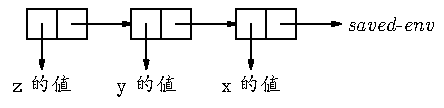
\includegraphics[scale=1.0]{nameless-env.pdf}\end{SCentered}

由于更改了环境接口,我们需要查看代码中所有依赖这套接口的地方。我们的解释器中使用
环境的只有两处:过程和 \Scribtexttt{value{-}of}。

修改过程规范时,只需把旧规范中的变量名移除:

\begin{EoplEquationInset}\begin{SVerbatim}\begin{SingleColumn}\Scribtexttt{(apply{-}procedure (procedure }\texMathInline{var}\Scribtexttt{}\mbox{\hphantom{\Scribtexttt{x}}}\Scribtexttt{}\texMathInline{body}\Scribtexttt{}\mbox{\hphantom{\Scribtexttt{x}}}\Scribtexttt{}\texMathInline{\rho}\Scribtexttt{) }\texMathInline{val}\Scribtexttt{)}

\Scribtexttt{= (value{-}of }\texMathInline{body}\Scribtexttt{}\mbox{\hphantom{\Scribtexttt{x}}}\Scribtexttt{(extend{-}nameless{-}env }\texMathInline{val}\Scribtexttt{}\mbox{\hphantom{\Scribtexttt{x}}}\Scribtexttt{}\texMathInline{\rho}\Scribtexttt{))}\end{SingleColumn}\end{SVerbatim}\end{EoplEquationInset}

\begin{EoplFigure}[!ht]


\begin{SCodeFlow}\begin{RktBlk}\begin{SingleColumn}\textbf{\Scribtexttt{nameless{-}environment{\hbox{\texttt{?}}}}} : \texMathInline{\mathit{SchemeVal} \to \mathit{Bool}}

\RktPn{(}\RktSym{define}\mbox{\hphantom{\Scribtexttt{x}}}\RktSym{nameless{-}environment{\hbox{\texttt{?}}}}

\mbox{\hphantom{\Scribtexttt{xx}}}\RktPn{(}\RktSym{lambda}\mbox{\hphantom{\Scribtexttt{x}}}\RktPn{(}\RktSym{x}\RktPn{)}

\mbox{\hphantom{\Scribtexttt{xxxx}}}\RktPn{(}\RktPn{(}\RktSym{list{-}of}\mbox{\hphantom{\Scribtexttt{x}}}\RktSym{exp{-}val{\hbox{\texttt{?}}}}\RktPn{)}\mbox{\hphantom{\Scribtexttt{x}}}\RktSym{x}\RktPn{)}\RktPn{)}\RktPn{)}

\mbox{\hphantom{\Scribtexttt{x}}}

\textbf{\Scribtexttt{empty{-}nameless{-}env}} : \texMathInline{\mathit{()} \to \mathit{Nameless\mbox{-}env}}

\RktPn{(}\RktSym{define}\mbox{\hphantom{\Scribtexttt{x}}}\RktSym{empty{-}nameless{-}env}

\mbox{\hphantom{\Scribtexttt{xx}}}\RktPn{(}\RktSym{lambda}\mbox{\hphantom{\Scribtexttt{x}}}\RktPn{(}\RktPn{)}\mbox{\hphantom{\Scribtexttt{x}}}\RktVal{{\textquotesingle}}\RktVal{(}\RktVal{)}\RktPn{)}\RktPn{)}

\mbox{\hphantom{\Scribtexttt{x}}}

\textbf{\Scribtexttt{extend{-}nameless{-}env}} : \texMathInline{\mathit{Expval} \times \mathit{Nameless\mbox{-}env} \to \mathit{Nameless\mbox{-}env}}

\RktPn{(}\RktSym{define}\mbox{\hphantom{\Scribtexttt{x}}}\RktSym{extend{-}nameless{-}env}

\mbox{\hphantom{\Scribtexttt{xx}}}\RktPn{(}\RktSym{lambda}\mbox{\hphantom{\Scribtexttt{x}}}\RktPn{(}\RktSym{val}\mbox{\hphantom{\Scribtexttt{x}}}\RktSym{nameless{-}env}\RktPn{)}

\mbox{\hphantom{\Scribtexttt{xxxx}}}\RktPn{(}\RktSym{cons}\mbox{\hphantom{\Scribtexttt{x}}}\RktSym{val}\mbox{\hphantom{\Scribtexttt{x}}}\RktSym{nameless{-}env}\RktPn{)}\RktPn{)}\RktPn{)}

\mbox{\hphantom{\Scribtexttt{x}}}

\textbf{\Scribtexttt{apply{-}nameless{-}env}} : \texMathInline{\mathit{Nameless\mbox{-}env} \times \mathit{Lexaddr} \to \mathit{DenVal}}

\RktPn{(}\RktSym{define}\mbox{\hphantom{\Scribtexttt{x}}}\RktSym{apply{-}nameless{-}env}

\mbox{\hphantom{\Scribtexttt{xx}}}\RktPn{(}\RktSym{lambda}\mbox{\hphantom{\Scribtexttt{x}}}\RktPn{(}\RktSym{nameless{-}env}\mbox{\hphantom{\Scribtexttt{x}}}\RktSym{n}\RktPn{)}

\mbox{\hphantom{\Scribtexttt{xxxx}}}\RktPn{(}\RktSym{list{-}ref}\mbox{\hphantom{\Scribtexttt{x}}}\RktSym{nameless{-}env}\mbox{\hphantom{\Scribtexttt{x}}}\RktSym{n}\RktPn{)}\RktPn{)}\RktPn{)}\end{SingleColumn}\end{RktBlk}\end{SCodeFlow}

\caption{无名环境
\index{hzuan2jing4@环境!wzu2ming2@无名|)idxdecorator{}{}}
\index{wzu2ming2huan2jing4@无名环境|)idxdecorator{}{}}\label{t:x28elem_x22figx2d3x2e17x22x29}}\end{EoplFigure}

这一规范的实现可定义为:

\begin{EoplCodeInset}\begin{SCodeFlow}\begin{RktBlk}\begin{SingleColumn}\textbf{\Scribtexttt{procedure}} : \texMathInline{\mathit{Nameless\mbox{-}exp} \times \mathit{Nameless\mbox{-}env} \to \mathit{Proc}}

\RktPn{(}\RktSym{define{-}datatype}\mbox{\hphantom{\Scribtexttt{x}}}\RktSym{proc}\mbox{\hphantom{\Scribtexttt{x}}}\RktSym{proc{\hbox{\texttt{?}}}}

\mbox{\hphantom{\Scribtexttt{xx}}}\RktPn{(}\RktSym{procedure}

\mbox{\hphantom{\Scribtexttt{xxx}}}\RktPn{(}\RktSym{body}\mbox{\hphantom{\Scribtexttt{x}}}\RktSym{expression{\hbox{\texttt{?}}}}\RktPn{)}

\mbox{\hphantom{\Scribtexttt{xxx}}}\RktPn{(}\RktSym{saved{-}nameless{-}env}\mbox{\hphantom{\Scribtexttt{x}}}\RktSym{nameless{-}environment{\hbox{\texttt{?}}}}\RktPn{)}\RktPn{)}\RktPn{)}

\mbox{\hphantom{\Scribtexttt{x}}}

\textbf{\Scribtexttt{apply{-}procedure}} : \texMathInline{\mathit{Proc} \times \mathit{ExpVal} \to \mathit{ExpVal}}

\RktPn{(}\RktSym{define}\mbox{\hphantom{\Scribtexttt{x}}}\RktSym{apply{-}procedure}

\mbox{\hphantom{\Scribtexttt{xx}}}\RktPn{(}\RktSym{lambda}\mbox{\hphantom{\Scribtexttt{x}}}\RktPn{(}\RktSym{proc1}\mbox{\hphantom{\Scribtexttt{x}}}\RktSym{val}\RktPn{)}

\mbox{\hphantom{\Scribtexttt{xxxx}}}\RktPn{(}\RktSym{cases}\mbox{\hphantom{\Scribtexttt{x}}}\RktSym{proc}\mbox{\hphantom{\Scribtexttt{x}}}\RktSym{proc1}

\mbox{\hphantom{\Scribtexttt{xxxxxx}}}\RktPn{(}\RktSym{procedure}

\mbox{\hphantom{\Scribtexttt{xxxxxxxx}}}\RktPn{(}\RktSym{body}\mbox{\hphantom{\Scribtexttt{x}}}\RktSym{saved{-}nameless{-}env}\RktPn{)}

\mbox{\hphantom{\Scribtexttt{xxxxxxxx}}}\RktPn{(}\RktSym{value{-}of}\mbox{\hphantom{\Scribtexttt{x}}}\RktSym{body}

\mbox{\hphantom{\Scribtexttt{xxxxxxxxxx}}}\RktPn{(}\RktSym{extend{-}nameless{-}env}\mbox{\hphantom{\Scribtexttt{x}}}\RktSym{val}\mbox{\hphantom{\Scribtexttt{x}}}\RktSym{saved{-}nameless{-}env}\RktPn{)}\RktPn{)}\RktPn{)}\RktPn{)}\RktPn{)}\RktPn{)}\end{SingleColumn}\end{RktBlk}\end{SCodeFlow}\end{EoplCodeInset}

\index{valueof@\textbf{\Scribtexttt{value{-}of}}!wzu2ming2ban3ben3@无名版本|(idxdecorator{}{}}
现在,我们可以写出 \Scribtexttt{value{-}of}。它的大部分与前一个解释器相同,只是原先使用
\Scribtexttt{env} 的地方现在用 \Scribtexttt{nameless{-}env}。但我们要处理新的部分:
\Scribtexttt{nameless{-}var{-}exp}、\Scribtexttt{nameless{-}let{-}exp} 和 \Scribtexttt{nameless{-}proc{-}exp},它们分别
取代对应的 \Scribtexttt{var{-}exp}、\Scribtexttt{let{-}exp} 和 \Scribtexttt{proc{-}exp}。其实现如
所示。\Scribtexttt{nameless{-}var{-}exp} 用于环境查询。\Scribtexttt{nameless{-}let{-}exp} 先求出式子右边的
\texMathInline{exp_1},然后用式子右边的值扩展环境,并在新环境内求主体的值。这和 \Scribtexttt{let} 所
做相同,只是没有变量。\Scribtexttt{nameless{-}proc} 生成一个 \Scribtexttt{proc},随后可供
\Scribtexttt{apply{-}procedure} 调用。
\index{valueof@\textbf{\Scribtexttt{value{-}of}}!wzu2ming2ban3ben3@无名版本|)idxdecorator{}{}}

\begin{EoplFigure}[!t]


\begin{SCodeFlow}\begin{RktBlk}\begin{SingleColumn}\textbf{\Scribtexttt{value{-}of}} : \texMathInline{\mathit{Nameless\mbox{-}exp} \times \mathit{Nameless\mbox{-}env} \to \mathit{ExpVal}}

\RktPn{(}\RktSym{define}\mbox{\hphantom{\Scribtexttt{x}}}\RktSym{value{-}of}

\mbox{\hphantom{\Scribtexttt{xx}}}\RktPn{(}\RktSym{lambda}\mbox{\hphantom{\Scribtexttt{x}}}\RktPn{(}\RktSym{exp}\mbox{\hphantom{\Scribtexttt{x}}}\RktSym{nameless{-}env}\RktPn{)}

\mbox{\hphantom{\Scribtexttt{xxxx}}}\RktPn{(}\RktSym{cases}\mbox{\hphantom{\Scribtexttt{x}}}\RktSym{expression}\mbox{\hphantom{\Scribtexttt{x}}}\RktSym{exp}

\mbox{\hphantom{\Scribtexttt{x}}}

\mbox{\hphantom{\Scribtexttt{xxxxxx}}}\RktPn{(}\RktSym{const{-}exp}\mbox{\hphantom{\Scribtexttt{x}}}\RktPn{(}\RktSym{num}\RktPn{)}\mbox{\hphantom{\Scribtexttt{x}}}\texMathInline{\ldots} \emph{同前} \texMathInline{\ldots}\RktPn{)}

\mbox{\hphantom{\Scribtexttt{xxxxxx}}}\RktPn{(}\RktSym{diff{-}exp}\mbox{\hphantom{\Scribtexttt{x}}}\RktPn{(}\RktSym{exp1}\mbox{\hphantom{\Scribtexttt{x}}}\RktSym{exp2}\RktPn{)}\mbox{\hphantom{\Scribtexttt{x}}}\texMathInline{\ldots} \emph{同前} \texMathInline{\ldots}\RktPn{)}

\mbox{\hphantom{\Scribtexttt{xxxxxx}}}\RktPn{(}\RktSym{zero{\hbox{\texttt{?}}}{-}exp}\mbox{\hphantom{\Scribtexttt{x}}}\RktPn{(}\RktSym{exp1}\RktPn{)}\mbox{\hphantom{\Scribtexttt{x}}}\texMathInline{\ldots} \emph{同前} \texMathInline{\ldots}\RktPn{)}

\mbox{\hphantom{\Scribtexttt{xxxxxx}}}\RktPn{(}\RktSym{if{-}exp}\mbox{\hphantom{\Scribtexttt{x}}}\RktPn{(}\RktSym{exp1}\mbox{\hphantom{\Scribtexttt{x}}}\RktSym{exp2}\mbox{\hphantom{\Scribtexttt{x}}}\RktSym{exp3}\RktPn{)}\mbox{\hphantom{\Scribtexttt{x}}}\texMathInline{\ldots} \emph{同前} \texMathInline{\ldots}\RktPn{)}

\mbox{\hphantom{\Scribtexttt{xxxxxx}}}\RktPn{(}\RktSym{call{-}exp}\mbox{\hphantom{\Scribtexttt{x}}}\RktPn{(}\RktSym{rator}\mbox{\hphantom{\Scribtexttt{x}}}\RktSym{rand}\RktPn{)}\mbox{\hphantom{\Scribtexttt{x}}}\texMathInline{\ldots} \emph{同前} \texMathInline{\ldots}\RktPn{)}

\mbox{\hphantom{\Scribtexttt{x}}}

\mbox{\hphantom{\Scribtexttt{xxxxxx}}}\RktPn{(}\RktSym{nameless{-}var{-}exp}\mbox{\hphantom{\Scribtexttt{x}}}\RktPn{(}\RktSym{n}\RktPn{)}

\mbox{\hphantom{\Scribtexttt{xxxxxxxx}}}\RktPn{(}\RktSym{apply{-}nameless{-}env}\mbox{\hphantom{\Scribtexttt{x}}}\RktSym{nameless{-}env}\mbox{\hphantom{\Scribtexttt{x}}}\RktSym{n}\RktPn{)}\RktPn{)}

\mbox{\hphantom{\Scribtexttt{x}}}

\mbox{\hphantom{\Scribtexttt{xxxxxx}}}\RktPn{(}\RktSym{nameless{-}let{-}exp}

\mbox{\hphantom{\Scribtexttt{xxxxxxxx}}}\RktPn{(}\RktSym{exp1}\mbox{\hphantom{\Scribtexttt{x}}}\RktSym{body}\RktPn{)}

\mbox{\hphantom{\Scribtexttt{xxxxxxxx}}}\RktPn{(}\RktSym{let}\mbox{\hphantom{\Scribtexttt{x}}}\RktPn{(}\RktPn{(}\RktSym{val}\mbox{\hphantom{\Scribtexttt{x}}}\RktPn{(}\RktSym{value{-}of}\mbox{\hphantom{\Scribtexttt{x}}}\RktSym{exp1}\mbox{\hphantom{\Scribtexttt{x}}}\RktSym{nameless{-}env}\RktPn{)}\RktPn{)}\RktPn{)}

\mbox{\hphantom{\Scribtexttt{xxxxxxxxxx}}}\RktPn{(}\RktSym{value{-}of}\mbox{\hphantom{\Scribtexttt{x}}}\RktSym{body}

\mbox{\hphantom{\Scribtexttt{xxxxxxxxxxxx}}}\RktPn{(}\RktSym{extend{-}nameless{-}env}\mbox{\hphantom{\Scribtexttt{x}}}\RktSym{val}\mbox{\hphantom{\Scribtexttt{x}}}\RktSym{nameless{-}env}\RktPn{)}\RktPn{)}\RktPn{)}\RktPn{)}

\mbox{\hphantom{\Scribtexttt{x}}}

\mbox{\hphantom{\Scribtexttt{xxxxxx}}}\RktPn{(}\RktSym{nameless{-}proc{-}exp}\mbox{\hphantom{\Scribtexttt{x}}}\RktPn{(}\RktSym{body}\RktPn{)}

\mbox{\hphantom{\Scribtexttt{xxxxxxxx}}}\RktPn{(}\RktSym{proc{-}val}

\mbox{\hphantom{\Scribtexttt{xxxxxxxxxx}}}\RktPn{(}\RktSym{procedure}\mbox{\hphantom{\Scribtexttt{x}}}\RktSym{body}\mbox{\hphantom{\Scribtexttt{x}}}\RktSym{nameless{-}env}\RktPn{)}\RktPn{)}\RktPn{)}

\mbox{\hphantom{\Scribtexttt{x}}}

\mbox{\hphantom{\Scribtexttt{xxxxxx}}}\RktPn{(}\RktSym{else}

\mbox{\hphantom{\Scribtexttt{xxxxxxxx}}}\RktPn{(}\RktSym{report{-}invalid{-}translated{-}expression}\mbox{\hphantom{\Scribtexttt{x}}}\RktSym{exp}\RktPn{)}\RktPn{)}\RktPn{)}\RktPn{)}\RktPn{)}\end{SingleColumn}\end{RktBlk}\end{SCodeFlow}

\caption{无名解释器的 \Scribtexttt{value{-}of}\label{t:x28elem_x22figx2d3x2e18x22x29}}

\noindent \index{valueof@\textbf{\Scribtexttt{value{-}of}}!wzu2ming2ban3ben3@无名版本|idxdecorator{}{}}\end{EoplFigure}

最后是新的 \Scribtexttt{value{-}of{-}program}:

\begin{EoplCodeInset}\begin{SCodeFlow}\begin{RktBlk}\begin{SingleColumn}\textbf{\Scribtexttt{value{-}of{-}program}} : \texMathInline{\mathit{Nameless\mbox{-}program} \to \mathit{ExpVal}}

\RktPn{(}\RktSym{define}\mbox{\hphantom{\Scribtexttt{x}}}\RktSym{value{-}of{-}program}

\mbox{\hphantom{\Scribtexttt{xx}}}\RktPn{(}\RktSym{lambda}\mbox{\hphantom{\Scribtexttt{x}}}\RktPn{(}\RktSym{pgm}\RktPn{)}

\mbox{\hphantom{\Scribtexttt{xxxx}}}\RktPn{(}\RktSym{cases}\mbox{\hphantom{\Scribtexttt{x}}}\RktSym{program}\mbox{\hphantom{\Scribtexttt{x}}}\RktSym{pgm}

\mbox{\hphantom{\Scribtexttt{xxxxxx}}}\RktPn{(}\RktSym{a{-}program}\mbox{\hphantom{\Scribtexttt{x}}}\RktPn{(}\RktSym{exp1}\RktPn{)}

\mbox{\hphantom{\Scribtexttt{xxxxxxxx}}}\RktPn{(}\RktSym{value{-}of}\mbox{\hphantom{\Scribtexttt{x}}}\RktSym{exp1}\mbox{\hphantom{\Scribtexttt{x}}}\RktPn{(}\RktSym{init{-}nameless{-}env}\RktPn{)}\RktPn{)}\RktPn{)}\RktPn{)}\RktPn{)}\RktPn{)}\end{SingleColumn}\end{RktBlk}\end{SCodeFlow}

\noindent \index{LETREC!wzu2ming2ban3ben3@无名版本|)idxdecorator{}{}}
\index{qzu4ming2@去名!LETREC@LETREC|)idxdecorator{}{}}
\index{bzian4liang4@变量!szheng1ming2@声明|)idxdecorator{}{}}\end{EoplCodeInset}

\begin{EoplExercise}\label{t:x28elem_x22ex3x2e38x22x29}\texMathInline{\textnormal{[}{\star}\textnormal{]}}\mbox{\hphantom{\Scribtexttt{x}}}\index{condbziao3da2shi4@\Scribtexttt{cond} 表达式|idxdecorator{}{}}
扩展词法地址翻译器和解释器,处理ex3.12 中的 \Scribtexttt{cond}。\end{EoplExercise}

\begin{EoplExercise}\label{t:x28elem_x22ex3x2e39x22x29}\texMathInline{\textnormal{[}{\star}\textnormal{]}}\mbox{\hphantom{\Scribtexttt{x}}}\index{unpackbziao3da2shi4@\Scribtexttt{unpack} 表达式|idxdecorator{}{}}
扩展词法地址翻译器和解释器,处理ex3.18 中的 \Scribtexttt{unpack}。\end{EoplExercise}

\begin{EoplExercise}\label{t:x28elem_x22ex3x2e40x22x29}\texMathInline{\textnormal{[}{\star}{\star}\textnormal{]}}\mbox{\hphantom{\Scribtexttt{x}}}\index{fzan1yi4@翻译!yzou3ming2dao4wu2ming2LETREC@有名到无名 LETREC|(idxdecorator{}{}}
扩展词法地址翻译器和解释器,处理 \Scribtexttt{letrec}。修改 \Scribtexttt{translation{-}of} 的上下文
参数,不仅记录每个绑定变量的名字,也记录变量是否由 \Scribtexttt{letrec} 绑定。对
\Scribtexttt{letrec} 绑定变量的引用,生成一种新的引用,名为 \Scribtexttt{nameless{-}letrec{-}var{-}exp}。
然后你可以继续用上面的无名环境表示,解释器则要以适当的方式处理\Shtt{nameless{-}letrec{-}var{-}exp}。\end{EoplExercise}

\begin{EoplExercise}\label{t:x28elem_x22ex3x2e41x22x29}\texMathInline{\textnormal{[}{\star}{\star}\textnormal{]}}\mbox{\hphantom{\Scribtexttt{x}}}\index{hzuan2jing4@环境!lze1pai2biao3shi4@肋排表示|(idxdecorator{}{}}
\index{tzui1li3gui1ze2@推理规则|(idxdecorator{}{}}
修改词法地址翻译器和解释器,像ex3.21 那样处理多参数的 \Scribtexttt{let} 表
达式、过程和过程调用。用肋排表示法(ex2.21)表示无名环境。在这种
表示法中,词法地址包含两个非负数:词深,指明跨越的等深线数目,与之前相同;位置,
指明变量在声明中的位置。
\index{hzuan2jing4@环境!lze1pai2biao3shi4@肋排表示|)idxdecorator{}{}}
\index{tzui1li3gui1ze2@推理规则|)idxdecorator{}{}}\end{EoplExercise}

\begin{EoplExercise}\label{t:x28elem_x22ex3x2e42x22x29}\texMathInline{\textnormal{[}{\star}{\star}{\star}\textnormal{]}}\mbox{\hphantom{\Scribtexttt{x}}}\index{szhu4ju4jie2gou4biao3shi4fa3@数据结构表示法!gzuo4cheng2zhi2@过程值|(idxdecorator{}{}}
\index{gzuo4cheng2zhi2Proc@过程值 (\texMathInline{\mathit{Proc}})!szhu4ju4jie2gou4biao3shi4@数据结构表示|(idxdecorator{}{}}
修改词法地址翻译器和解释器,使用ex3.26 中的瘦身过程表示法。要如此,
你不能在 \Scribtexttt{(extend{-}senv }\texMathInline{var}\Scribtexttt{ }\texMathInline{senv}\Scribtexttt{)} 中翻译过程的主体,而是在一个新的静
态环境中,它指明了各个变量在瘦身表示中的位置。
\index{szhu4ju4jie2gou4biao3shi4fa3@数据结构表示法!gzuo4cheng2zhi2@过程值|)idxdecorator{}{}}
\index{gzuo4cheng2zhi2Proc@过程值 (\texMathInline{\mathit{Proc}})!szhu4ju4jie2gou4biao3shi4@数据结构表示|)idxdecorator{}{}}
\index{fzan1yi4@翻译!yzou3ming2dao4wu2ming2LETREC@有名到无名 LETREC|)idxdecorator{}{}}\end{EoplExercise}

\begin{EoplExercise}\label{t:x28elem_x22ex3x2e43x22x29}\texMathInline{\textnormal{[}{\star}{\star}{\star}\textnormal{]}}\mbox{\hphantom{\Scribtexttt{x}}}\index{szheng1ming2@声明!gzuo4cheng2@过程|(idxdecorator{}{}}
\index{yzi3zhi1guo4cheng2@已知过程|(idxdecorator{}{}}
\index{gzuo4cheng2sheng1ming2@过程声明|(idxdecorator{}{}}
翻译器不止能记录变量的名字。例如,考虑程序

\begin{EoplCodeInset}\begin{SVerbatim}\begin{SingleColumn}\Scribtexttt{let x = 3}

\Scribtexttt{in let f = proc (y) {-}(y,x)}

\Scribtexttt{}\mbox{\hphantom{\Scribtexttt{xxx}}}\Scribtexttt{in (f 13)}\end{SingleColumn}\end{SVerbatim}\end{EoplCodeInset}

这里,不必运行我们就能看出:在过程调用处,\Scribtexttt{f} 绑定到一个过程,其主体为
\Scribtexttt{{-}(y,x)},\Scribtexttt{x} 的值与过程创建处相同。因此我们完全可以避免在环境中查找
\Scribtexttt{f}。扩展翻译器,记录“已知过程”,生成代码,避免在
调用这样的过程时搜索环境。\end{EoplExercise}

\begin{EoplExercise}\label{t:x28elem_x22ex3x2e44x22x29}\texMathInline{\textnormal{[}{\star}{\star}{\star}\textnormal{]}}\mbox{\hphantom{\Scribtexttt{x}}}在前一个例子中,\Scribtexttt{f} 的唯一用途是作为一个已知过程。因此,由表达式 \Scribtexttt{proc (y)
{-}(y,x)} 产生的过程从未使用。修改翻译器,避免产生这样的过程。
\index{szheng1ming2@声明!gzuo4cheng2@过程|)idxdecorator{}{}}
\index{yzi3zhi1guo4cheng2@已知过程|)idxdecorator{}{}}
\index{gzuo4cheng2sheng1ming2@过程声明|)idxdecorator{}{}}\end{EoplExercise}

\sectionNewpage

\Ssection{状态}{状态}\label{t:x28part_x22statex22x29}



\Ssubsection{计算的效果}{计算的效果}\label{t:x28part_x22s4x2e1x22x29}

\index{jzi4suan4xiao4guo3@计算效果|idxdecorator{}{}}
\index{yzin3yong4@引用|(idxdecorator{}{}}
到目前为止,我们只考虑了计算产生的\emph{值} (\emph{value}),但是计算也
有\emph{效果} (\emph{effect}):它可以读取,打印,修改内存或者文件系统的状态。在现实世
界中,我们\emph{总是}对效果很感兴趣:如果一次计算不显示答案,那对我们完全没用!

产生值和产生效果有何区别?效果是\emph{全局性} (\emph{global}) 的,整个计算都能看到。效
果\emph{感染}整个计算(故意用双关语)。

\index{bzang3ding4Binding@绑定 (Binding)!bzian4liang4@变量|idxdecorator{}{}}
\index{gzong4xiang3bian4liang4@共享变量|idxdecorator{}{}}
我们主要关心一种效果:给内存中的位置赋值。赋值与绑定有何区别?我们已经知道,绑定
是局部的,但\index{fzu4zhi2@赋值|idxdecorator{}{}}变量赋值有可能是全局的。那是在本不相关的几
部分计算之间\emph{共享} (\emph{share}) \index{bzian4liang4@变量!gzong4xiang3@共享|idxdecorator{}{}}
值。如果两个过程知道内存中的同一位置,它们就能共享信息。如果把信息留在已知位置,
同一个过程就能在当前调用和后续调用之间共享信息。

\index{wzei4zhi4@位置|idxdecorator{}{}}
\index{kze3cun2chu3zhi2@可存储值|idxdecorator{}{}}
我们把内存建模为从\emph{位置} (\emph{location}) 到值集合的的有限映射,称值集合
为\emph{可存储值} (\emph{storable values})。出于历史原因,我们称之为\emph{存
储器} (\emph{store})。通常,一种语言中的可存储值与表达值相同,但不总是这样。这个选择是语言设计
的一部分。\index{czun2chu3qi4@存储器|idxdecorator{}{}}

代表内存位置的数据结构叫做\emph{引用} (\emph{reference})。位置是内存中可用来存值的地方,
引用是指向那个地方的数据结构。位置和引用的区别可以这样类比:位置就像文件,引用就
像一个URL。URL指向一个文件,文件包含一些数据。类似地,引用指代一个位置,位置包含
一些数据。

\index{zzuo3zhi2@左值|idxdecorator{}{}}
引用有时候又叫\emph{左值} (\emph{L{-}values})。这名字反映了这种数据结构与赋值语句左边变
量的联系。类似地,表达值,比如赋值语句右边表达式的值,叫做\emph{右值} (\emph{R{-}values})。
\index{yzou4zhi2@右值|idxdecorator{}{}}

我们考虑两种带有存储器的语言设计。这些设计叫做\emph{显式引
用} (\emph{explicit reference}) 和\emph{隐式引用} (\emph{implicit reference})。
\index{yzin3yong4@引用|)idxdecorator{}{}}

\Ssubsection{EXPLICIT{-}REFS:显式引用语言}{EXPLICIT{-}REFS:显式引用语言}\label{t:x28part_x22s4x2e2x22x29}

\index{EXPLICITREFS@EXPLICIT{-}REFS|(idxdecorator{}{}}
\index{yzin3yong4@引用!xzian3shi4@显式|(idxdecorator{}{}}
在这种设计中,我们添加引用,作为另一种表达值。那么,我们有:

\begin{Subflow}\Iidentity{\begin{align*}\mathit{ExpVal} &= \mathit{Int} + \mathit{Bool} + \mathit{Proc} + \mathit{Ref(ExpVal)} \\
\mathit{DenVal} &= \mathit{ExpVal}\end{align*}}

这里,\texMathInline{\mathit{Ref(ExpVal)}}表示包含表达值的位置引用集合。\end{Subflow}

我们沿用语言中的绑定数据结构,但是添加三个新操作,用来创建和使用引用。

\begin{itemize}\atItemizeStart

\item \Scribtexttt{newref},分配新的位置,返回其引用。
\index{fzen1pei4@分配!czun2chu3qi4zhong1de@存储器中的|idxdecorator{}{}}

\item \Scribtexttt{deref},\emph{解引用} (\emph{deference}) :返回引用指向位置处的内容。
\index{jzie3yin3yong4@解引用|idxdecorator{}{}}

\item \Scribtexttt{setref},改变引用指向位置处的内容。
\index{kze3bian4xing4@可变性|(idxdecorator{}{}}\end{itemize}

我们把得到的语言称作 EXPLICIT{-}REFS。让我们用这些结构写几个程序。

下面是两个过程 \Scribtexttt{even} 和 \Scribtexttt{odd}。它们取一参数,但是忽略它,并根据位置
\Scribtexttt{x} 处的内容是偶数还是奇数返回 1 或 0。它们不是通过直接传递数据来通信,而是改
变共享变量的内容。\index{gzong4xiang3bian4liang4@共享变量|idxdecorator{}{}}\index{bzian4liang4@变量!gzong4xiang3@共享|idxdecorator{}{}}

这个程序判断 13 是否为奇数,并返回 1。过程 \Scribtexttt{even} 和 \Scribtexttt{odd} 不引用它们的实
参,而是查看绑定到 \Scribtexttt{x} 的位置中的内容。

\begin{Subflow}\begin{EoplCodeInset}\begin{SVerbatim}\begin{SingleColumn}\Scribtexttt{let x = newref (0)}

\Scribtexttt{in letrec even(dummy)}

\Scribtexttt{}\mbox{\hphantom{\Scribtexttt{xxxxxxxxxxx}}}\Scribtexttt{= if zero{\hbox{\texttt{?}}} (deref(x))}

\Scribtexttt{}\mbox{\hphantom{\Scribtexttt{xxxxxxxxxxxxx}}}\Scribtexttt{then 1}

\Scribtexttt{}\mbox{\hphantom{\Scribtexttt{xxxxxxxxxxxxx}}}\Scribtexttt{else begin}

\Scribtexttt{}\mbox{\hphantom{\Scribtexttt{xxxxxxxxxxxxxxxxxxx}}}\Scribtexttt{setref(x, {-}(deref(x), 1));}

\Scribtexttt{}\mbox{\hphantom{\Scribtexttt{xxxxxxxxxxxxxxxxxxx}}}\Scribtexttt{(odd 888)}

\Scribtexttt{}\mbox{\hphantom{\Scribtexttt{xxxxxxxxxxxxxxxxxx}}}\Scribtexttt{end}

\Scribtexttt{}\mbox{\hphantom{\Scribtexttt{xxxxxxxxxx}}}\Scribtexttt{odd(dummy)}

\Scribtexttt{}\mbox{\hphantom{\Scribtexttt{xxxxxxxxxxx}}}\Scribtexttt{= if zero{\hbox{\texttt{?}}} (deref(x))}

\Scribtexttt{}\mbox{\hphantom{\Scribtexttt{xxxxxxxxxxxxx}}}\Scribtexttt{then 0}

\Scribtexttt{}\mbox{\hphantom{\Scribtexttt{xxxxxxxxxxxxx}}}\Scribtexttt{else begin}

\Scribtexttt{}\mbox{\hphantom{\Scribtexttt{xxxxxxxxxxxxxxxxxxx}}}\Scribtexttt{setref(x, {-}(deref(x), 1));}

\Scribtexttt{}\mbox{\hphantom{\Scribtexttt{xxxxxxxxxxxxxxxxxxx}}}\Scribtexttt{(even 888)}

\Scribtexttt{}\mbox{\hphantom{\Scribtexttt{xxxxxxxxxxxxxxxxxx}}}\Scribtexttt{end}

\Scribtexttt{}\mbox{\hphantom{\Scribtexttt{xxx}}}\Scribtexttt{in begin setref(x,13); (odd 888) end}\end{SingleColumn}\end{SVerbatim}\end{EoplCodeInset}

这个程序使用多声明的 \Scribtexttt{letrec}(ex3.32)和 \Scribtexttt{begin} 表达式
(ex4.4)。\Scribtexttt{begin} 表达式按顺序求每个子表达式的值,并返
回最后一个表达式的值。
\index{beginbziao3da2shi4@\Scribtexttt{begin} 表达式|idxdecorator{}{}}\end{Subflow}

为了同我们的单参数语言保持一致,我们给 \Scribtexttt{even} 和 \Scribtexttt{odd} 传一个无用参数;如
果我们的过程支持任意数量的参数(ex3.21),这些过程的参数就可以去
掉。

当两个过程需要分享很多量时,这种通信方式很方便;只需给某些随调用而改变的量赋值。
同样地,一个过程可能通过一长串调用间接调用另一过程。二者可以通过一个共享变量直接
交换数据,居间的过程不需要知道它。因此,以共享变量通信可作为一种隐藏信息的方式。

\index{szi1you3bian4liang4@私有变量|idxdecorator{}{}}
\index{bzian4liang4@变量!szi1you3@私有|idxdecorator{}{}}
赋值的另一用途是通过私有变量创建隐藏状态。例如:

\begin{EoplCodeInset}\begin{SVerbatim}\begin{SingleColumn}\label{t:x28elem_x22gx2dcounterx22x29}\Scribtexttt{let g = let counter = newref(0)}

\Scribtexttt{}\mbox{\hphantom{\Scribtexttt{xxxxxxxx}}}\Scribtexttt{in proc (dummy)}

\Scribtexttt{}\mbox{\hphantom{\Scribtexttt{xxxxxxxxxxxx}}}\Scribtexttt{begin}

\Scribtexttt{}\mbox{\hphantom{\Scribtexttt{xxxxxxxxxxxxx}}}\Scribtexttt{setref(counter, {-}(deref(counter), {-}1));}

\Scribtexttt{}\mbox{\hphantom{\Scribtexttt{xxxxxxxxxxxxx}}}\Scribtexttt{deref(counter)}

\Scribtexttt{}\mbox{\hphantom{\Scribtexttt{xxxxxxxxxxxx}}}\Scribtexttt{end}

\Scribtexttt{in let a = (g 11)}

\Scribtexttt{}\mbox{\hphantom{\Scribtexttt{xxx}}}\Scribtexttt{in let b = (g 11)}

\Scribtexttt{}\mbox{\hphantom{\Scribtexttt{xxxxxx}}}\Scribtexttt{in {-}(a,b)}\end{SingleColumn}\end{SVerbatim}\end{EoplCodeInset}

这里,过程 \Scribtexttt{g} 保留了一个私有变量,用来存储 \Scribtexttt{g} 被调用的次数。因此,第一次
调用 \Scribtexttt{g} 返回 1,第二次返回 2,整个程序的值为 {-}1。

\index{gzong4xiang3bian4liang4@共享变量|(idxdecorator{}{}}
下图是 \Scribtexttt{g} 绑定时所在的环境。可以认为,这是在 \Scribtexttt{g} 的不同调用之间共享信息。
Scheme 过程 \Scribtexttt{gensym} 用这种技术创建唯一符号。

\begin{EoplFigure*}[!ht]

\noindent \begin{SCentered}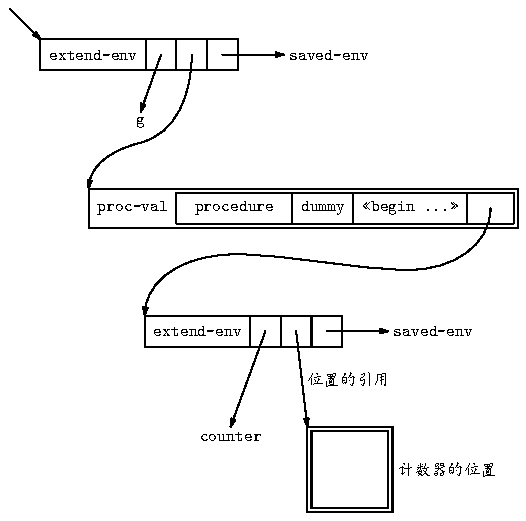
\includegraphics[scale=0.95]{g-bound.pdf}\end{SCentered}

\noindent \index{gzong4xiang3bian4liang4@共享变量|)idxdecorator{}{}}
\index{bzian4liang4@变量!gzong4xiang3@共享|idxdecorator{}{}}\end{EoplFigure*}

\begin{EoplExercise}\label{t:x28elem_x22ex4x2e1x22x29}\texMathInline{\textnormal{[}{\star}\textnormal{]}}\mbox{\hphantom{\Scribtexttt{x}}}这个程序如果写成下面这样会怎样?

\begin{EoplCodeInset}\begin{SVerbatim}\begin{SingleColumn}\Scribtexttt{let g = proc (dummy)}

\Scribtexttt{}\mbox{\hphantom{\Scribtexttt{xxxxxxxxxx}}}\Scribtexttt{let counter = newref(0)}

\Scribtexttt{}\mbox{\hphantom{\Scribtexttt{xxxxxxxxxx}}}\Scribtexttt{in begin}

\Scribtexttt{}\mbox{\hphantom{\Scribtexttt{xxxxxxxxxxxxx}}}\Scribtexttt{setref(counter, {-}(deref(counter), {-}1));}

\Scribtexttt{}\mbox{\hphantom{\Scribtexttt{xxxxxxxxxxxxx}}}\Scribtexttt{deref(counter)}

\Scribtexttt{}\mbox{\hphantom{\Scribtexttt{xxxxxxxxxx}}}\Scribtexttt{end}

\Scribtexttt{in let a = (g 11)}

\Scribtexttt{}\mbox{\hphantom{\Scribtexttt{xxx}}}\Scribtexttt{in let b = (g 11)}

\Scribtexttt{}\mbox{\hphantom{\Scribtexttt{xxxxxx}}}\Scribtexttt{in {-}(a,b)}\end{SingleColumn}\end{SVerbatim}\end{EoplCodeInset}\end{EoplExercise}

在EXPLICIT{-}REFS中,我们可以存储任何表达值。引用也是表达值。这意味着我们可以在一
个位置存储引用。考虑下面的程序:\index{kze3cun2chu3zhi2@可存储值|idxdecorator{}{}}

\begin{EoplCodeInset}\begin{SVerbatim}\begin{SingleColumn}\Scribtexttt{let x = newref(newref(0))}

\Scribtexttt{in begin}

\Scribtexttt{}\mbox{\hphantom{\Scribtexttt{xxxx}}}\Scribtexttt{setref(deref(x), 11);}

\Scribtexttt{}\mbox{\hphantom{\Scribtexttt{xxxx}}}\Scribtexttt{deref(deref(x))}

\Scribtexttt{end}\end{SingleColumn}\end{SVerbatim}\end{EoplCodeInset}

这段程序分配了一个新位置,内容为 0。然后,它将 \Scribtexttt{x} 绑定到一个位置,其内容为指
向第一个位置的引用。因此,\Scribtexttt{deref(x)} 的值是第一个位置的引用。那么程序求
\Scribtexttt{setref} 的值时,会修改第一个位置,整个程序返回 11。

\Ssubsubsection{存储器传递规范}{存储器传递规范}\label{t:x28part_x22s4x2e2x2e1x22x29}

\index{valueof@\textbf{\Scribtexttt{value{-}of}}!EXPLICITREFS@EXPLICIT{-}REFS|(idxdecorator{}{}}
在我们的语言中,任何表达式都可以有效果。要定义这些效果,我们需要描述每次求值使用
什么样的存储器,以及求值如何修改存储器。

在规范中,我们用 \texMathInline{\sigma} 表示任一存储器,用 \texMathInline{\text{[}l=v\text{]}\sigma} 表
示另一存储器,除了将位置 \texMathInline{l} 映射到 \texMathInline{v}外,它与 \texMathInline{\sigma} 相同。有时,涉及
\texMathInline{\sigma} 的某个具体值时,我们称之为存储器的\emph{状态} (\emph{state})。

我们使用\emph{存储器传递规范} (\emph{store{-}passing specifications})。在存储器传递规范
中,存储器作为显式参数传递给 \Scribtexttt{value{-}of},并作为 \Scribtexttt{value{-}of} 的结果返回。那
么我们可以写:\index{czun2chu3qi4chuan2di4gui1fan4@存储器传递规范|idxdecorator{}{}}
\texMathDisplay{\Scribtexttt{(value{-}of }\texMathInline{exp_1}\Scribtexttt{ }\texMathInline{\rho}\Scribtexttt{ }\texMathInline{\sigma_0}\Scribtexttt{)} = \Scribtexttt{(}\texMathInline{val_1}\Scribtexttt{,}\texMathInline{\sigma_1}\Scribtexttt{)}}


\noindent \begin{Subflow}它断言在环境为 \texMathInline{\rho},存储器状态为 \texMathInline{\sigma_0} 时,表达式 \texMathInline{exp_1} 的返回值
为 \texMathInline{val_1},并且可能把存储器修改为另一状态 \texMathInline{\sigma_1}。\end{Subflow}

这样我们就能写出 \Scribtexttt{const{-}exp} 之类的无效果操作:
\texMathDisplay{\Scribtexttt{(value{-}of (const{-}exp }\texMathInline{n}\Scribtexttt{) }\texMathInline{\rho}\Scribtexttt{ }\texMathInline{\sigma}\Scribtexttt{)} = \Scribtexttt{(}\texMathInline{n}\Scribtexttt{,}\texMathInline{\sigma}\Scribtexttt{)}}


\noindent \begin{Subflow}以此表明求表达式的值不会修改存储器。\end{Subflow}

\Scribtexttt{diff{-}exp} 的规范展示了如何定义有顺序的行为。
\texMathDisplay{\infer{\Scribtexttt{(value{-}of (diff{-}exp }\texMathInline{exp_1}\Scribtexttt{ }\texMathInline{exp_2}\Scribtexttt{) }\texMathInline{\rho}\Scribtexttt{ }\texMathInline{\sigma_0}\Scribtexttt{)} =
       \Scribtexttt{(}\texMathInline{\lceil\lfloor val_1 \rfloor - \lfloor val_2 \rfloor\rceil}\Scribtexttt{,}\texMathInline{\sigma_2}\Scribtexttt{)}}
      {\begin{alignedat}{-1}
         \Scribtexttt{(value{-}of (diff{-}exp }\texMathInline{exp_1}\Scribtexttt{) }\texMathInline{\rho}\Scribtexttt{ }\texMathInline{\sigma_0}\Scribtexttt{)} &= \Scribtexttt{(}\texMathInline{val_1}\Scribtexttt{,}\texMathInline{\sigma_1}\Scribtexttt{)} \\
         \Scribtexttt{(value{-}of (diff{-}exp }\texMathInline{exp_2}\Scribtexttt{) }\texMathInline{\rho}\Scribtexttt{ }\texMathInline{\sigma_1}\Scribtexttt{)} &= \Scribtexttt{(}\texMathInline{val_2}\Scribtexttt{,}\texMathInline{\sigma_2}\Scribtexttt{)}
       \end{alignedat}}}


\noindent \begin{Subflow}这里,我们从状态为 \texMathInline{\sigma_0} 的存储器开始,首先求 \texMathInline{exp_1} 的值。\texMathInline{exp_1}
返回值为 \texMathInline{val_1},但它可能有效果,把存储器状态修改为 \texMathInline{\sigma_1}。然后我们从
\texMathInline{exp_1} 修改过的存储器{---}{---}也就是 \texMathInline{\sigma_1}{---}{---}开始,求 \texMathInline{exp_2} 的值。
\texMathInline{exp_2} 同样返回一个值 \texMathInline{val_2},并把存储器状态修改为 \texMathInline{\sigma_2}。之后,整
个表达式返回 \texMathInline{val_1 - val2},对存储器不再有任何效果,所以存储器状态留在
\texMathInline{\sigma_2}。\end{Subflow}

再来试试条件表达式。
\texMathDisplay{\infer{\begin{alignedat}{-1}
         &\mbox{\hphantom{\Scribtexttt{x}}}\Scribtexttt{(value{-}of (if{-}exp }\texMathInline{exp_1}\Scribtexttt{ }\texMathInline{exp_2}\Scribtexttt{ }\texMathInline{exp_3}\Scribtexttt{) }\texMathInline{\rho}\Scribtexttt{ }\texMathInline{\sigma_0}\Scribtexttt{) } \\
         &\hphantom{xx}= \begin{cases}
                          \Scribtexttt{(value{-}of }\texMathInline{exp_2}\Scribtexttt{ }\texMathInline{\rho}\Scribtexttt{ }\texMathInline{\sigma_1}\Scribtexttt{)} & 若 \Scribtexttt{(expval{-}{\Stttextmore}bool }\texMathInline{val_1}\Scribtexttt{)} = \Scribtexttt{\#t} \\
                          \Scribtexttt{(value{-}of }\texMathInline{exp_3}\Scribtexttt{ }\texMathInline{\rho}\Scribtexttt{ }\texMathInline{\sigma_1}\Scribtexttt{)} & 若 \Scribtexttt{(expval{-}{\Stttextmore}bool }\texMathInline{val_1}\Scribtexttt{)} = \Scribtexttt{\#f} \hphantom{x}
                        \end{cases}
       \end{alignedat}}
      {\Scribtexttt{(value{-}of }\texMathInline{exp_1}\Scribtexttt{ }\texMathInline{\rho}\Scribtexttt{ }\texMathInline{\sigma_0}\Scribtexttt{)} = \Scribtexttt{(}\texMathInline{val_1}\Scribtexttt{,}\texMathInline{\sigma_1}\Scribtexttt{)}}}

一个 \Scribtexttt{if{-}exp} 从状态 \texMathInline{\sigma_0} 开始,求条件表达式 \texMathInline{exp_1} 的值,返回值
\texMathInline{val_1},将存储器状态修改为 \texMathInline{\sigma_1}。整个表达式的结果可能是 \texMathInline{exp_2} 或
\texMathInline{exp_3} 的结果,二者都在当前环境 \texMathInline{\rho} 和 \texMathInline{exp_1} 留下的存储器状态
\texMathInline{\sigma_1} 中求值。

\begin{EoplExercise}\label{t:x28elem_x22ex4x2e2x22x29}\texMathInline{\textnormal{[}{\star}\textnormal{]}}\mbox{\hphantom{\Scribtexttt{x}}}写出 \Scribtexttt{zero{\hbox{\texttt{?}}}{-}exp} 的规范。\end{EoplExercise}

\begin{EoplExercise}\label{t:x28elem_x22ex4x2e3x22x29}\texMathInline{\textnormal{[}{\star}\textnormal{]}}\mbox{\hphantom{\Scribtexttt{x}}}写出 \Scribtexttt{call{-}exp} 的规范。\end{EoplExercise}

\begin{EoplExercise}\label{t:x28elem_x22ex4x2e4x22x29}\texMathInline{\textnormal{[}{\star}{\star}\textnormal{]}}\mbox{\hphantom{\Scribtexttt{x}}}\index{beginbziao3da2shi4@\Scribtexttt{begin} 表达式|idxdecorator{}{}}
写出 \Scribtexttt{begin} 表达式的规范。
\texMathDisplay{\mathit{Expression} ::= \Scribtexttt{begin }\texMathInline{\mathit{Expression}}\Scribtexttt{ }\texMathInline{\{}\Scribtexttt{; }\texMathInline{\mathit{Expression}}\texMathInline{\}^{*}}\Scribtexttt{ end}}

\Scribtexttt{begin} 表达式包含一个或多个分号分隔的子表达式,按顺序求这些子表达的值,并返
回最后一个的结果。\end{EoplExercise}

\begin{EoplExercise}\label{t:x28elem_x22ex4x2e5x22x29}\texMathInline{\textnormal{[}{\star}{\star}\textnormal{]}}\mbox{\hphantom{\Scribtexttt{x}}}\index{listbziao3da2shi4@\Scribtexttt{list} 表达式|idxdecorator{}{}}
写出 \Scribtexttt{list}(ex3.10)的规范。\end{EoplExercise}

\Ssubsubsection{定义显式引用操作}{定义显式引用操作}\label{t:x28part_x22s4x2e2x2e2x22x29}

\index{fzen1pei4@分配!czun2chu3qi4zhong1de@存储器中的|(idxdecorator{}{}}
在 EXPLICIT{-}REFS 中,我们必须定义三个操作:\Scribtexttt{newref}、\Scribtexttt{deref} 和
\Scribtexttt{setref}。它们的语法为:

\Iidentity{\begin{align*}\mathit{Expression} &::= \Scribtexttt{newref (}\Iidentity{\mathit{Expression}}\Scribtexttt{)} \\[-3pt]
  &\mathrel{\phantom{::=}} \fbox{\Scribtexttt{newref{-}exp (exp1)}} \\[5pt]
\mathit{Expression} &::= \Scribtexttt{deref (}\Iidentity{\mathit{Expression}}\Scribtexttt{)} \\[-3pt]
  &\mathrel{\phantom{::=}} \fbox{\Scribtexttt{deref{-}exp (exp1)}} \\[5pt]
\mathit{Expression} &::= \Scribtexttt{setref (}\Iidentity{\mathit{Expression}}\Scribtexttt{ , }\Iidentity{\mathit{Expression}}\Scribtexttt{)} \\[-3pt]
  &\mathrel{\phantom{::=}} \fbox{\Scribtexttt{setref{-}exp (exp1 exp2)}}\end{align*}}

这些操作的行为定义如下。
\texMathDisplay{\infer{\Scribtexttt{(value{-}of (newref{-}exp }\texMathInline{exp}\Scribtexttt{) }\texMathInline{\rho}\Scribtexttt{ }\texMathInline{\sigma_0}\Scribtexttt{) =}\Scribtexttt{
}\Scribtexttt{((ref{-}val }\texMathInline{l}\Scribtexttt{),[}\texMathInline{l}\Scribtexttt{=}\texMathInline{val}\Scribtexttt{]}\texMathInline{\sigma_1}\Scribtexttt{)}}
      {\Scribtexttt{(value{-}of }\texMathInline{exp}\Scribtexttt{ }\texMathInline{\rho}\Scribtexttt{ }\texMathInline{\sigma_0}\Scribtexttt{)} = \Scribtexttt{(}\texMathInline{val}\Scribtexttt{,}\texMathInline{\sigma_1}\Scribtexttt{)} \quad l \notin \text{dom}(\sigma_1)}}

这条规则是说:\Scribtexttt{newref{-}exp} 求出操作数的值,得到一个存储器,然后分配一个新位置
\texMathInline{l},将参数值 \texMathInline{val} 放到这一位置,以此来扩展那个存储器。然后它返回新位置
\texMathInline{l} 的引用。这意味着 \texMathInline{l} 不在 \texMathInline{\sigma_1} 的定义域内。
\index{jzie3yin3yong4@解引用|idxdecorator{}{}}
\texMathDisplay{\infer{\Scribtexttt{(value{-}of (deref{-}exp }\texMathInline{exp}\Scribtexttt{) }\texMathInline{\rho}\Scribtexttt{ }\texMathInline{\sigma_0}\Scribtexttt{) =}\Scribtexttt{
}\Scribtexttt{(}\texMathInline{\sigma_1(l)}\Scribtexttt{,}\texMathInline{\sigma_1}\Scribtexttt{)}}
      {\Scribtexttt{(value{-}of }\texMathInline{exp}\Scribtexttt{ }\texMathInline{\rho}\Scribtexttt{ }\texMathInline{\sigma_0}\Scribtexttt{)} = \Scribtexttt{(}\texMathInline{val}\Scribtexttt{,}\texMathInline{\sigma_1}\Scribtexttt{)}}}

这条规则是说:\Scribtexttt{deref{-}exp} 求出操作数的值,然后把存储器状态改为 \texMathInline{\sigma_1}。
参数的值应是位置 \texMathInline{l} 的引用。然后 \Scribtexttt{deref{-}exp} 返回 \texMathInline{\sigma_1} 中 \texMathInline{l} 处
的内容,不再更改存储器。
\texMathDisplay{\infer{\Scribtexttt{(value{-}of (setref{-}exp }\texMathInline{exp_1}\Scribtexttt{ }\texMathInline{exp_2}\Scribtexttt{) }\texMathInline{\rho}\Scribtexttt{ }\texMathInline{\sigma_0}\Scribtexttt{) =}\Scribtexttt{
}\Scribtexttt{(}\texMathInline{\lceil 23 \rceil}\Scribtexttt{,[}\texMathInline{l}\Scribtexttt{=}\texMathInline{val}\Scribtexttt{]}\texMathInline{\sigma_2}\Scribtexttt{)}}
      {\begin{gathered}
        \Scribtexttt{(value{-}of }\texMathInline{exp_1}\Scribtexttt{ }\texMathInline{\rho}\Scribtexttt{ }\texMathInline{\sigma_0}\Scribtexttt{)} = \Scribtexttt{(}\texMathInline{l}\Scribtexttt{,}\texMathInline{\sigma_1}\Scribtexttt{)} \\
        \Scribtexttt{(value{-}of }\texMathInline{exp_2}\Scribtexttt{ }\texMathInline{\rho}\Scribtexttt{ }\texMathInline{\sigma_1}\Scribtexttt{)} = \Scribtexttt{(}\texMathInline{val}\Scribtexttt{,}\texMathInline{\sigma_2}\Scribtexttt{)}
       \end{gathered}}}

\index{kze3bian4xing4@可变性|idxdecorator{}{}}
这条规则是说:\Scribtexttt{setref{-}exp} 从左到右求操作数的值。第一个操作数的值必须是某个位
置 \texMathInline{l} 的引用;然后 \Scribtexttt{setref{-}exp} 把第二个参数的值 \texMathInline{val} 放到位置 \texMathInline{l} 处,
以此更新存储器。\Scribtexttt{setref{-}exp} 应该返回什么呢?它可以返回任何值。为了强调这一选
择的随意性,我们让它返回 23。因为我们对 \Scribtexttt{setref{-}exp} 的返回值不感兴趣,我们说
这个表达式的执行\emph{求效果} (\emph{for effect}) 而不求值。
\index{jzi4suan4xiao4guo3@计算效果|idxdecorator{}{}}
\index{qziu2xiao4guo3@求效果|idxdecorator{}{}}
\index{valueof@\textbf{\Scribtexttt{value{-}of}}!EXPLICITREFS@EXPLICIT{-}REFS|)idxdecorator{}{}}

\begin{EoplExercise}\label{t:x28elem_x22ex4x2e6x22x29}\texMathInline{\textnormal{[}{\star}\textnormal{]}}\mbox{\hphantom{\Scribtexttt{x}}}修改上面的规则,让 \Scribtexttt{setref{-}exp} 返回右边表达式的值。\end{EoplExercise}

\begin{EoplExercise}\label{t:x28elem_x22ex4x2e7x22x29}\texMathInline{\textnormal{[}{\star}\textnormal{]}}\mbox{\hphantom{\Scribtexttt{x}}}修改上面的规则,让 \Scribtexttt{setref{-}exp} 返回位置的原内容。
\index{fzen1pei4@分配!czun2chu3qi4zhong1de@存储器中的|)idxdecorator{}{}}\end{EoplExercise}

\Ssubsubsection{实现}{实现}\label{t:x28part_x22s4x2e2x2e3x22x29}

\index{czun2chu3qi4@存储器|(idxdecorator{}{}}
迄今为止,我们使用的规范语言可以轻松描述有效果计算的期望行为,但是它没有体现存储
器的一个要点:引用最终指向现实世界的内存中某一真实的位置。因为我们只有一个现实世
界,我们的程序只能记录存储器的一个状态 \texMathInline{\sigma}。

在我们的实现中,我们利用这一事实,用 Scheme 中的存储器建模存储器。这样,我们就能
用 Scheme 中的效果建模效果。

我们用一个 Scheme 值表示存储器状态,但是我们不像规范建议的那样直接传递和返回它,
相反,我们在一个全局变量中记录状态,实现代码中的所有过程都能访问它。这很像示例程
序 \Scribtexttt{even/odd} 使用共享位置,而不是直接传递参数。使用单一全局变量时,我们也几
乎不需要理解 Scheme 中的效果。

我们还是要选择如何用 Scheme 值建模存储器。我们选择的可能是最简单的模型:以表达值
列表作为存储器,以代表列表位置的数字表示引用。分配新引用就是给列表末尾添加新值;
更新存储器则建模为按需复制列表的一大部分。代码如 和
fig{-}4.2 所示。

\begin{EoplFigure}[!ht]

\begin{SCodeFlow}\begin{RktBlk}\begin{SingleColumn}\textbf{\Scribtexttt{empty{-}store}} : \texMathInline{() \to \mathit{Sto}}

\RktPn{(}\RktSym{define}\mbox{\hphantom{\Scribtexttt{x}}}\RktSym{empty{-}store}

\mbox{\hphantom{\Scribtexttt{xx}}}\RktPn{(}\RktSym{lambda}\mbox{\hphantom{\Scribtexttt{x}}}\RktPn{(}\RktPn{)}\mbox{\hphantom{\Scribtexttt{x}}}\RktVal{{\textquotesingle}}\RktVal{(}\RktVal{)}\RktPn{)}\RktPn{)}

\mbox{\hphantom{\Scribtexttt{x}}}

\emph{\textbf{用法} : Scheme 变量,包含存储器当前的状态。初始值无意义。}

\RktPn{(}\RktSym{define}\mbox{\hphantom{\Scribtexttt{x}}}\RktSym{the{-}store}\mbox{\hphantom{\Scribtexttt{x}}}\RktVal{{\textquotesingle}}\RktVal{uninitialized}\RktPn{)}

\mbox{\hphantom{\Scribtexttt{x}}}

\textbf{\Scribtexttt{get{-}store}} : \texMathInline{() \to \mathit{Sto}}

\RktPn{(}\RktSym{define}\mbox{\hphantom{\Scribtexttt{x}}}\RktSym{get{-}store}

\mbox{\hphantom{\Scribtexttt{xx}}}\RktPn{(}\RktSym{lambda}\mbox{\hphantom{\Scribtexttt{x}}}\RktPn{(}\RktPn{)}\mbox{\hphantom{\Scribtexttt{x}}}\RktSym{the{-}store}\RktPn{)}\RktPn{)}

\mbox{\hphantom{\Scribtexttt{x}}}

\textbf{\Scribtexttt{initialize{-}store{\hbox{\texttt{!}}}}} : \texMathInline{() \to \mathit{Unspecified}}

\emph{\textbf{用法} : \Scribtexttt{(initialize{-}store{\hbox{\texttt{!}}})} 将存储器设为空。}

\RktPn{(}\RktSym{define}\mbox{\hphantom{\Scribtexttt{x}}}\RktSym{initialize{-}store{\hbox{\texttt{!}}}}

\mbox{\hphantom{\Scribtexttt{xx}}}\RktPn{(}\RktSym{lambda}\mbox{\hphantom{\Scribtexttt{x}}}\RktPn{(}\RktPn{)}

\mbox{\hphantom{\Scribtexttt{xxxx}}}\RktPn{(}\RktSym{set{\hbox{\texttt{!}}}}\mbox{\hphantom{\Scribtexttt{x}}}\RktSym{the{-}store}\mbox{\hphantom{\Scribtexttt{x}}}\RktPn{(}\RktSym{empty{-}store}\RktPn{)}\RktPn{)}\RktPn{)}\RktPn{)}

\mbox{\hphantom{\Scribtexttt{x}}}

\textbf{\Scribtexttt{reference{\hbox{\texttt{?}}}}} : \texMathInline{\mathit{SchemeVal} \to \mathit{Bool}}

\RktPn{(}\RktSym{define}\mbox{\hphantom{\Scribtexttt{x}}}\RktSym{reference{\hbox{\texttt{?}}}}

\mbox{\hphantom{\Scribtexttt{xx}}}\RktPn{(}\RktSym{lambda}\mbox{\hphantom{\Scribtexttt{x}}}\RktPn{(}\RktSym{v}\RktPn{)}

\mbox{\hphantom{\Scribtexttt{xxxx}}}\RktPn{(}\RktSym{integer{\hbox{\texttt{?}}}}\mbox{\hphantom{\Scribtexttt{x}}}\RktSym{v}\RktPn{)}\RktPn{)}\RktPn{)}

\mbox{\hphantom{\Scribtexttt{x}}}

\textbf{\Scribtexttt{newref}} : \texMathInline{\mathit{ExpVal} \to \mathit{Ref}}

\RktPn{(}\RktSym{define}\mbox{\hphantom{\Scribtexttt{x}}}\RktSym{newref}

\mbox{\hphantom{\Scribtexttt{xx}}}\RktPn{(}\RktSym{lambda}\mbox{\hphantom{\Scribtexttt{x}}}\RktPn{(}\RktSym{val}\RktPn{)}

\mbox{\hphantom{\Scribtexttt{xxxx}}}\RktPn{(}\RktSym{let}\mbox{\hphantom{\Scribtexttt{x}}}\RktPn{(}\RktPn{(}\RktSym{next{-}ref}\mbox{\hphantom{\Scribtexttt{x}}}\RktPn{(}\RktSym{length}\mbox{\hphantom{\Scribtexttt{x}}}\RktSym{the{-}store}\RktPn{)}\RktPn{)}\RktPn{)}

\mbox{\hphantom{\Scribtexttt{xxxxxx}}}\RktPn{(}\RktSym{set{\hbox{\texttt{!}}}}\mbox{\hphantom{\Scribtexttt{x}}}\RktSym{the{-}store}\mbox{\hphantom{\Scribtexttt{x}}}\RktPn{(}\RktSym{append}\mbox{\hphantom{\Scribtexttt{x}}}\RktSym{the{-}store}\mbox{\hphantom{\Scribtexttt{x}}}\RktPn{(}\RktSym{list}\mbox{\hphantom{\Scribtexttt{x}}}\RktSym{val}\RktPn{)}\RktPn{)}\RktPn{)}

\mbox{\hphantom{\Scribtexttt{xxxxxx}}}\RktSym{next{-}ref}\RktPn{)}\RktPn{)}\RktPn{)}

\mbox{\hphantom{\Scribtexttt{x}}}

\textbf{\Scribtexttt{deref}} : \texMathInline{\mathit{Ref} \to \mathit{ExpVal}}

\RktPn{(}\RktSym{define}\mbox{\hphantom{\Scribtexttt{x}}}\RktSym{deref}

\mbox{\hphantom{\Scribtexttt{xx}}}\RktPn{(}\RktSym{lambda}\mbox{\hphantom{\Scribtexttt{x}}}\RktPn{(}\RktSym{ref}\RktPn{)}

\mbox{\hphantom{\Scribtexttt{xxxx}}}\RktPn{(}\RktSym{list{-}ref}\mbox{\hphantom{\Scribtexttt{x}}}\RktSym{the{-}store}\mbox{\hphantom{\Scribtexttt{x}}}\RktSym{ref}\RktPn{)}\RktPn{)}\RktPn{)}\end{SingleColumn}\end{RktBlk}\end{SCodeFlow}

\caption{拙劣的存储器模型\label{t:x28elem_x22figx2d4x2e1x22x29}}\end{EoplFigure}

\begin{EoplFigure}[!ht]

\begin{SCodeFlow}\begin{RktBlk}\begin{SingleColumn}\textbf{\Scribtexttt{setref{\hbox{\texttt{!}}}}} : \texMathInline{\mathit{Ref} \times \mathit{ExpVal} \to \mathit{Unspecified}}

\emph{\textbf{用法} : 除了把位置 \Scribtexttt{ref} 的值设为 \Scribtexttt{val},\Scribtexttt{the{-}store} 与原状态相同。}

\RktPn{(}\RktSym{define}\mbox{\hphantom{\Scribtexttt{x}}}\RktSym{setref{\hbox{\texttt{!}}}}

\mbox{\hphantom{\Scribtexttt{xx}}}\RktPn{(}\RktSym{lambda}\mbox{\hphantom{\Scribtexttt{x}}}\RktPn{(}\RktSym{ref}\mbox{\hphantom{\Scribtexttt{x}}}\RktSym{val}\RktPn{)}

\mbox{\hphantom{\Scribtexttt{xxxx}}}\RktPn{(}\RktSym{set{\hbox{\texttt{!}}}}\mbox{\hphantom{\Scribtexttt{x}}}\RktSym{the{-}store}

\mbox{\hphantom{\Scribtexttt{xxxxxx}}}\RktPn{(}\RktSym{letrec}

\mbox{\hphantom{\Scribtexttt{xxxxxxxx}}}\RktPn{(}\RktPn{(}\RktSym{setref{-}inner}

\mbox{\hphantom{\Scribtexttt{xxxxxxxxxxx}}}\emph{\textbf{用法} : 返回一列表,除了位置 ref1 处}

\mbox{\hphantom{\Scribtexttt{xxxxxxxxxxx}}}\emph{值为 val,与 store1 相同。}

\mbox{\hphantom{\Scribtexttt{xxxxxxxxxxx}}}\RktPn{(}\RktSym{lambda}\mbox{\hphantom{\Scribtexttt{x}}}\RktPn{(}\RktSym{store1}\mbox{\hphantom{\Scribtexttt{x}}}\RktSym{ref1}\RktPn{)}

\mbox{\hphantom{\Scribtexttt{xxxxxxxxxxxxx}}}\RktPn{(}\RktSym{cond}

\mbox{\hphantom{\Scribtexttt{xxxxxxxxxxxxxxx}}}\RktPn{(}\RktPn{(}\RktSym{null{\hbox{\texttt{?}}}}\mbox{\hphantom{\Scribtexttt{x}}}\RktSym{store1}\RktPn{)}

\mbox{\hphantom{\Scribtexttt{xxxxxxxxxxxxxxxxx}}}\RktPn{(}\RktSym{report{-}invalid{-}reference}\mbox{\hphantom{\Scribtexttt{x}}}\RktSym{ref}\mbox{\hphantom{\Scribtexttt{x}}}\RktSym{the{-}store}\RktPn{)}\RktPn{)}

\mbox{\hphantom{\Scribtexttt{xxxxxxxxxxxxxxx}}}\RktPn{(}\RktPn{(}\RktSym{zero{\hbox{\texttt{?}}}}\mbox{\hphantom{\Scribtexttt{x}}}\RktSym{ref1}\RktPn{)}

\mbox{\hphantom{\Scribtexttt{xxxxxxxxxxxxxxxxx}}}\RktPn{(}\RktSym{cons}\mbox{\hphantom{\Scribtexttt{x}}}\RktSym{val}\mbox{\hphantom{\Scribtexttt{x}}}\RktPn{(}\RktSym{cdr}\mbox{\hphantom{\Scribtexttt{x}}}\RktSym{store1}\RktPn{)}\RktPn{)}\RktPn{)}

\mbox{\hphantom{\Scribtexttt{xxxxxxxxxxxxxxx}}}\RktPn{(}\RktSym{else}

\mbox{\hphantom{\Scribtexttt{xxxxxxxxxxxxxxxxx}}}\RktPn{(}\RktSym{cons}

\mbox{\hphantom{\Scribtexttt{xxxxxxxxxxxxxxxxxxx}}}\RktPn{(}\RktSym{car}\mbox{\hphantom{\Scribtexttt{x}}}\RktSym{store1}\RktPn{)}

\mbox{\hphantom{\Scribtexttt{xxxxxxxxxxxxxxxxxxx}}}\RktPn{(}\RktSym{setref{-}inner}

\mbox{\hphantom{\Scribtexttt{xxxxxxxxxxxxxxxxxxxxx}}}\RktPn{(}\RktSym{cdr}\mbox{\hphantom{\Scribtexttt{x}}}\RktSym{store1}\RktPn{)}\mbox{\hphantom{\Scribtexttt{x}}}\RktPn{(}\RktSym{\mbox{{-}}}\mbox{\hphantom{\Scribtexttt{x}}}\RktSym{ref1}\mbox{\hphantom{\Scribtexttt{x}}}\RktVal{1}\RktPn{)}\RktPn{)}\RktPn{)}\RktPn{)}\RktPn{)}\RktPn{)}\RktPn{)}\RktPn{)}

\mbox{\hphantom{\Scribtexttt{xxxxxxxx}}}\RktPn{(}\RktSym{setref{-}inner}\mbox{\hphantom{\Scribtexttt{x}}}\RktSym{the{-}store}\mbox{\hphantom{\Scribtexttt{x}}}\RktSym{ref}\RktPn{)}\RktPn{)}\RktPn{)}\RktPn{)}\RktPn{)}\end{SingleColumn}\end{RktBlk}\end{SCodeFlow}

\caption{拙劣的存储器模型,续\label{t:x28elem_x22figx2d4x2e2x22x29}}\end{EoplFigure}

这种表示极其低效。一般的内存操作大致在常数时间内完成,但是采用我们的表示,这些操
作所需的时间与存储器大小成正比。当然,真正实现起来不会这么做,但这足以达到我们的
目的。

我们给表达值数据类型新增一种变体 \Scribtexttt{ref{-}val},然后修改 \Scribtexttt{value{-}of{-}program},
在每次求值之前初始化存储器。

\begin{Subflow}\begin{EoplCodeInset}\begin{SCodeFlow}\begin{RktBlk}\begin{SingleColumn}\textbf{\Scribtexttt{value{-}of{-}program}} : \texMathInline{\mathit{Program} \to \mathit{SchemeVal}}

\RktPn{(}\RktSym{define}\mbox{\hphantom{\Scribtexttt{x}}}\RktSym{value{-}of{-}program}

\mbox{\hphantom{\Scribtexttt{xx}}}\RktPn{(}\RktSym{lambda}\mbox{\hphantom{\Scribtexttt{x}}}\RktPn{(}\RktSym{pgm}\RktPn{)}

\mbox{\hphantom{\Scribtexttt{xxxx}}}\RktPn{(}\RktSym{initialize{-}store{\hbox{\texttt{!}}}}\RktPn{)}

\mbox{\hphantom{\Scribtexttt{xxxx}}}\RktPn{(}\RktSym{cases}\mbox{\hphantom{\Scribtexttt{x}}}\RktSym{program}\mbox{\hphantom{\Scribtexttt{x}}}\RktSym{pgm}

\mbox{\hphantom{\Scribtexttt{xxxxxx}}}\RktPn{(}\RktSym{a{-}program}\mbox{\hphantom{\Scribtexttt{x}}}\RktPn{(}\RktSym{exp1}\RktPn{)}

\mbox{\hphantom{\Scribtexttt{xxxxxxxx}}}\RktPn{(}\RktSym{value{-}of}\mbox{\hphantom{\Scribtexttt{x}}}\RktSym{exp1}\mbox{\hphantom{\Scribtexttt{x}}}\RktPn{(}\RktSym{init{-}env}\RktPn{)}\RktPn{)}\RktPn{)}\RktPn{)}\RktPn{)}\RktPn{)}\end{SingleColumn}\end{RktBlk}\end{SCodeFlow}\end{EoplCodeInset}

现在,我们可以写出 \Scribtexttt{value{-}of} 中与 \Scribtexttt{newref}、\Scribtexttt{deref} 和 \Scribtexttt{setref} 相
关的语句。这些语句如 所示。\end{Subflow}

我们可以给该系统添加一些\label{t:x28elem_x22tracex2dinstrumentx22x29}辅助过程,把环境、过程和存
储器转换为更易读的形式,也可以改善系统,在代码中的关键位置打印消息。我们还使用过
程把环境、过程和存储器转换为更易读的形式。得出的日志详细描述了系统的动作。典型例
子如 和 fig{-}4.5 所示。此外,这一跟踪日志还表明,
差值表达式的参数按从左到右的顺序求值。
\index{EXPLICITREFS@EXPLICIT{-}REFS|)idxdecorator{}{}}
\index{yzin3yong4@引用!xzian3shi4@显式|)idxdecorator{}{}}
\index{czun2chu3qi4@存储器|)idxdecorator{}{}}

\begin{EoplExercise}\label{t:x28elem_x22ex4x2e8x22x29}\texMathInline{\textnormal{[}{\star}\textnormal{]}}\mbox{\hphantom{\Scribtexttt{x}}}指出我们实现的存储器中,到底是哪些操作花费了线性时间而非常数时间。\end{EoplExercise}

\begin{EoplExercise}\label{t:x28elem_x22ex4x2e9x22x29}\texMathInline{\textnormal{[}{\star}\textnormal{]}}\mbox{\hphantom{\Scribtexttt{x}}}用 Scheme 向量表示存储器,从而实现常数时间操作。用这种表示会失去什么?\end{EoplExercise}

\begin{EoplExercise}\label{t:x28elem_x22ex4x2e10x22x29}\texMathInline{\textnormal{[}{\star}\textnormal{]}}\mbox{\hphantom{\Scribtexttt{x}}}\index{beginbziao3da2shi4@\Scribtexttt{begin} 表达式|idxdecorator{}{}}
实现\{ex4.4\} 中定义的 \Scribtexttt{begin} 表达式。\end{EoplExercise}

\begin{EoplExercise}\label{t:x28elem_x22ex4x2e11x22x29}\texMathInline{\textnormal{[}{\star}\textnormal{]}}\mbox{\hphantom{\Scribtexttt{x}}}\index{listbziao3da2shi4@\Scribtexttt{list} 表达式|idxdecorator{}{}}
实现ex4.5 中的 \Scribtexttt{list}。\end{EoplExercise}

\begin{EoplExercise}\label{t:x28elem_x22ex4x2e12x22x29}\texMathInline{\textnormal{[}{\star}{\star}{\star}\textnormal{]}}\mbox{\hphantom{\Scribtexttt{x}}}\index{valueof@\textbf{\Scribtexttt{value{-}of}}!EXPLICITREFS@EXPLICIT{-}REFS|(idxdecorator{}{}}
像解释器中展示的,我们对存储器的理解基于 Scheme 效果的含义。具体地说,我们得知道
在 Scheme 程序中这些效果\emph{何时}产生。我们可以写出更贴合规范的解释器,从而避
免这种依赖。在这一解释器中,\Scribtexttt{value{-}of} 同时返回值和存储器,就像规范中那样。这
一解释器的片段如 所示。我们称之为\emph{传递存储器的解释器} (\emph{store{-}passing
interpreter})。补全这个解释器,处理整个 EXPLICIT{-}REFS 语言。

过程可能修改存储器时,不仅返回通常的值,还要返回一个新存储器。它们包含在名为
\Scribtexttt{answer} 的数据类型之中。完成这个 \Scribtexttt{value{-}of} 的定义。
\index{valueof@\textbf{\Scribtexttt{value{-}of}}!EXPLICITREFS@EXPLICIT{-}REFS|)idxdecorator{}{}}\end{EoplExercise}

\begin{EoplExercise}\label{t:x28elem_x22ex4x2e13x22x29}\texMathInline{\textnormal{[}{\star}{\star}{\star}\textnormal{]}}\mbox{\hphantom{\Scribtexttt{x}}}\index{dzuo1can1shu4guo4cheng2@多参数过程|(idxdecorator{}{}}
扩展前一道练习中的解释器,支持多参数过程。
\index{dzuo1can1shu4guo4cheng2@多参数过程|)idxdecorator{}{}}\end{EoplExercise}

\begin{EoplFigure}[!ht]

\begin{SCodeFlow}\begin{RktBlk}\begin{SingleColumn}\mbox{\hphantom{\Scribtexttt{xxxx}}}\RktPn{(}\RktSym{newref{-}exp}\RktMeta{}

\mbox{\hphantom{\Scribtexttt{xxxx}}}\RktMeta{}\mbox{\hphantom{\Scribtexttt{x}}}\RktMeta{}\RktPn{(}\RktSym{exp1}\RktPn{)}\RktMeta{}

\mbox{\hphantom{\Scribtexttt{xxxx}}}\RktMeta{}\mbox{\hphantom{\Scribtexttt{x}}}\RktMeta{}\RktPn{(}\RktSym{let}\RktMeta{}\mbox{\hphantom{\Scribtexttt{x}}}\RktMeta{}\RktPn{(}\RktPn{(}\RktSym{v1}\RktMeta{}\mbox{\hphantom{\Scribtexttt{x}}}\RktMeta{}\RktPn{(}\RktSym{value{-}of}\RktMeta{}\mbox{\hphantom{\Scribtexttt{x}}}\RktMeta{}\RktSym{exp1}\RktMeta{}\mbox{\hphantom{\Scribtexttt{x}}}\RktMeta{}\RktSym{env}\RktPn{)}\RktPn{)}\RktPn{)}\RktMeta{}

\mbox{\hphantom{\Scribtexttt{xxxx}}}\RktMeta{}\mbox{\hphantom{\Scribtexttt{xxx}}}\RktMeta{}\RktPn{(}\RktSym{ref{-}val}\RktMeta{}\mbox{\hphantom{\Scribtexttt{x}}}\RktMeta{}\RktPn{(}\RktSym{newref}\RktMeta{}\mbox{\hphantom{\Scribtexttt{x}}}\RktMeta{}\RktSym{v1}\RktPn{)}\RktPn{)}\RktPn{)}\RktPn{)}\RktMeta{}

\mbox{\hphantom{\Scribtexttt{xxxx}}}\RktMeta{~}

\mbox{\hphantom{\Scribtexttt{xxxx}}}\RktMeta{}\RktPn{(}\RktSym{deref{-}exp}\RktMeta{}

\mbox{\hphantom{\Scribtexttt{xxxx}}}\RktMeta{}\mbox{\hphantom{\Scribtexttt{x}}}\RktMeta{}\RktPn{(}\RktSym{exp1}\RktPn{)}\RktMeta{}

\mbox{\hphantom{\Scribtexttt{xxxx}}}\RktMeta{}\mbox{\hphantom{\Scribtexttt{x}}}\RktMeta{}\RktPn{(}\RktSym{let}\RktMeta{}\mbox{\hphantom{\Scribtexttt{x}}}\RktMeta{}\RktPn{(}\RktPn{(}\RktSym{v1}\RktMeta{}\mbox{\hphantom{\Scribtexttt{x}}}\RktMeta{}\RktPn{(}\RktSym{value{-}of}\RktMeta{}\mbox{\hphantom{\Scribtexttt{x}}}\RktMeta{}\RktSym{exp1}\RktMeta{}\mbox{\hphantom{\Scribtexttt{x}}}\RktMeta{}\RktSym{env}\RktPn{)}\RktPn{)}\RktPn{)}\RktMeta{}

\mbox{\hphantom{\Scribtexttt{xxxx}}}\RktMeta{}\mbox{\hphantom{\Scribtexttt{xxx}}}\RktMeta{}\RktPn{(}\RktSym{let}\RktMeta{}\mbox{\hphantom{\Scribtexttt{x}}}\RktMeta{}\RktPn{(}\RktPn{(}\RktSym{ref1}\RktMeta{}\mbox{\hphantom{\Scribtexttt{x}}}\RktMeta{}\RktPn{(}\RktSym{expval{-}{\Stttextmore}ref}\RktMeta{}\mbox{\hphantom{\Scribtexttt{x}}}\RktMeta{}\RktSym{v1}\RktPn{)}\RktPn{)}\RktPn{)}\RktMeta{}

\mbox{\hphantom{\Scribtexttt{xxxx}}}\RktMeta{}\mbox{\hphantom{\Scribtexttt{xxxxx}}}\RktMeta{}\RktPn{(}\RktSym{deref}\RktMeta{}\mbox{\hphantom{\Scribtexttt{x}}}\RktMeta{}\RktSym{ref1}\RktPn{)}\RktPn{)}\RktPn{)}\RktPn{)}\RktMeta{}

\mbox{\hphantom{\Scribtexttt{xxxx}}}\RktMeta{~}

\mbox{\hphantom{\Scribtexttt{xxxx}}}\RktMeta{}\RktPn{(}\RktSym{setref{-}exp}\RktMeta{}

\mbox{\hphantom{\Scribtexttt{xxxx}}}\RktMeta{}\mbox{\hphantom{\Scribtexttt{x}}}\RktMeta{}\RktPn{(}\RktSym{exp1}\RktMeta{}\mbox{\hphantom{\Scribtexttt{x}}}\RktMeta{}\RktSym{exp2}\RktPn{)}\RktMeta{}

\mbox{\hphantom{\Scribtexttt{xxxx}}}\RktMeta{}\mbox{\hphantom{\Scribtexttt{x}}}\RktMeta{}\RktPn{(}\RktSym{let}\RktMeta{}\mbox{\hphantom{\Scribtexttt{x}}}\RktMeta{}\RktPn{(}\RktPn{(}\RktSym{ref}\RktMeta{}\mbox{\hphantom{\Scribtexttt{x}}}\RktMeta{}\RktPn{(}\RktSym{expval{-}{\Stttextmore}ref}\RktMeta{}\mbox{\hphantom{\Scribtexttt{x}}}\RktMeta{}\RktPn{(}\RktSym{value{-}of}\RktMeta{}\mbox{\hphantom{\Scribtexttt{x}}}\RktMeta{}\RktSym{exp1}\RktMeta{}\mbox{\hphantom{\Scribtexttt{x}}}\RktMeta{}\RktSym{env}\RktPn{)}\RktPn{)}\RktPn{)}\RktPn{)}\RktMeta{}

\mbox{\hphantom{\Scribtexttt{xxxx}}}\RktMeta{}\mbox{\hphantom{\Scribtexttt{xxx}}}\RktMeta{}\RktPn{(}\RktSym{let}\RktMeta{}\mbox{\hphantom{\Scribtexttt{x}}}\RktMeta{}\RktPn{(}\RktPn{(}\RktSym{val2}\RktMeta{}\mbox{\hphantom{\Scribtexttt{x}}}\RktMeta{}\RktPn{(}\RktSym{value{-}of}\RktMeta{}\mbox{\hphantom{\Scribtexttt{x}}}\RktMeta{}\RktSym{exp2}\RktMeta{}\mbox{\hphantom{\Scribtexttt{x}}}\RktMeta{}\RktSym{env}\RktPn{)}\RktPn{)}\RktPn{)}\RktMeta{}

\mbox{\hphantom{\Scribtexttt{xxxx}}}\RktMeta{}\mbox{\hphantom{\Scribtexttt{xxxxx}}}\RktMeta{}\RktPn{(}\RktSym{begin}\RktMeta{}

\mbox{\hphantom{\Scribtexttt{xxxx}}}\RktMeta{}\mbox{\hphantom{\Scribtexttt{xxxxxxx}}}\RktMeta{}\RktPn{(}\RktSym{setref{\hbox{\texttt{!}}}}\RktMeta{}\mbox{\hphantom{\Scribtexttt{x}}}\RktMeta{}\RktSym{ref}\RktMeta{}\mbox{\hphantom{\Scribtexttt{x}}}\RktMeta{}\RktSym{val2}\RktPn{)}\RktMeta{}

\mbox{\hphantom{\Scribtexttt{xxxx}}}\RktMeta{}\mbox{\hphantom{\Scribtexttt{xxxxxxx}}}\RktMeta{}\RktPn{(}\RktSym{num{-}val}\RktMeta{}\mbox{\hphantom{\Scribtexttt{x}}}\RktMeta{}\RktVal{23}\RktPn{)}\RktPn{)}\RktPn{)}\RktPn{)}\RktPn{)}\RktMeta{}\end{SingleColumn}\end{RktBlk}\end{SCodeFlow}

\caption{\Scribtexttt{value{-}of} 的显式引用操作语句
\index{jzie3yin3yong4@解引用|idxdecorator{}{}}\label{t:x28elem_x22figx2d4x2e3x22x29}}\end{EoplFigure}

\begin{EoplFigure}\begin{SVerbatim}\begin{SingleColumn}\Scribtexttt{}\mbox{\hphantom{\Scribtexttt{x}}}

\Scribtexttt{{\Stttextmore} (run "}

\Scribtexttt{let x = newref(22)}

\Scribtexttt{in let f = proc (z) let zz = newref({-}(z,deref(x)))}

\Scribtexttt{}\mbox{\hphantom{\Scribtexttt{xxxxxxxxxxxxxxxxxxxx}}}\Scribtexttt{in deref(zz)}

\Scribtexttt{}\mbox{\hphantom{\Scribtexttt{xxx}}}\Scribtexttt{in {-}((f 66), (f 55))")}

\Scribtexttt{}\mbox{\hphantom{\Scribtexttt{x}}}

\Scribtexttt{进入 let x}

\Scribtexttt{newref{\hbox{\texttt{:}}} 分配位置 0}

\Scribtexttt{进入 let x 主体,环境 =}

\Scribtexttt{((x \#(struct{\hbox{\texttt{:}}}ref{-}val 0))}

\Scribtexttt{}\mbox{\hphantom{\Scribtexttt{x}}}\Scribtexttt{(i \#(struct{\hbox{\texttt{:}}}num{-}val 1))}

\Scribtexttt{}\mbox{\hphantom{\Scribtexttt{x}}}\Scribtexttt{(v \#(struct{\hbox{\texttt{:}}}num{-}val 5))}

\Scribtexttt{}\mbox{\hphantom{\Scribtexttt{x}}}\Scribtexttt{(x \#(struct{\hbox{\texttt{:}}}num{-}val 10)))}

\Scribtexttt{存储器 =}

\Scribtexttt{((0 \#(struct{\hbox{\texttt{:}}}num{-}val 22)))}

\Scribtexttt{}\mbox{\hphantom{\Scribtexttt{x}}}

\Scribtexttt{进入 let f}

\Scribtexttt{进入 let f 主体,环境 =}

\Scribtexttt{((f}

\Scribtexttt{}\mbox{\hphantom{\Scribtexttt{xx}}}\Scribtexttt{(procedure}

\Scribtexttt{}\mbox{\hphantom{\Scribtexttt{xxx}}}\Scribtexttt{z}

\Scribtexttt{}\mbox{\hphantom{\Scribtexttt{xxx}}}\Scribtexttt{{\hbox{\texttt{.}}}{\hbox{\texttt{.}}}{\hbox{\texttt{.}}}}

\Scribtexttt{}\mbox{\hphantom{\Scribtexttt{xxx}}}\Scribtexttt{((x \#(struct{\hbox{\texttt{:}}}ref{-}val 0))}

\Scribtexttt{}\mbox{\hphantom{\Scribtexttt{xxxx}}}\Scribtexttt{(i \#(struct{\hbox{\texttt{:}}}num{-}val 1))}

\Scribtexttt{}\mbox{\hphantom{\Scribtexttt{xxxx}}}\Scribtexttt{(v \#(struct{\hbox{\texttt{:}}}num{-}val 5))}

\Scribtexttt{}\mbox{\hphantom{\Scribtexttt{xxxx}}}\Scribtexttt{(x \#(struct{\hbox{\texttt{:}}}num{-}val 10)))))}

\Scribtexttt{}\mbox{\hphantom{\Scribtexttt{x}}}\Scribtexttt{(x \#(struct{\hbox{\texttt{:}}}ref{-}val 0))}

\Scribtexttt{}\mbox{\hphantom{\Scribtexttt{x}}}\Scribtexttt{(i \#(struct{\hbox{\texttt{:}}}num{-}val 1))}

\Scribtexttt{}\mbox{\hphantom{\Scribtexttt{x}}}\Scribtexttt{(v \#(struct{\hbox{\texttt{:}}}num{-}val 5))}

\Scribtexttt{}\mbox{\hphantom{\Scribtexttt{x}}}\Scribtexttt{(x \#(struct{\hbox{\texttt{:}}}num{-}val 10)))}

\Scribtexttt{存储器 =}

\Scribtexttt{((0 \#(struct{\hbox{\texttt{:}}}num{-}val 22)))}

\Scribtexttt{}\mbox{\hphantom{\Scribtexttt{x}}}

\Scribtexttt{进入 proc z 主体,环境 =}

\Scribtexttt{((z \#(struct{\hbox{\texttt{:}}}num{-}val 66))}

\Scribtexttt{}\mbox{\hphantom{\Scribtexttt{x}}}\Scribtexttt{(x \#(struct{\hbox{\texttt{:}}}ref{-}val 0))}

\Scribtexttt{}\mbox{\hphantom{\Scribtexttt{x}}}\Scribtexttt{(i \#(struct{\hbox{\texttt{:}}}num{-}val 1))}

\Scribtexttt{}\mbox{\hphantom{\Scribtexttt{x}}}\Scribtexttt{(v \#(struct{\hbox{\texttt{:}}}num{-}val 5))}

\Scribtexttt{}\mbox{\hphantom{\Scribtexttt{x}}}\Scribtexttt{(x \#(struct{\hbox{\texttt{:}}}num{-}val 10)))}

\Scribtexttt{存储器 =}

\Scribtexttt{((0 \#(struct{\hbox{\texttt{:}}}num{-}val 22)))}\end{SingleColumn}\end{SVerbatim}

\caption{EXPLICIT{-}REFS的求值跟踪日志\label{t:x28elem_x22figx2d4x2e4x22x29}}\end{EoplFigure}

\begin{EoplFigure}\begin{SVerbatim}\begin{SingleColumn}\Scribtexttt{}\mbox{\hphantom{\Scribtexttt{x}}}

\Scribtexttt{进入 let zz}

\Scribtexttt{newref{\hbox{\texttt{:}}} 分配位置 1}

\Scribtexttt{进入 let zz 主体,环境 =}

\Scribtexttt{((zz \#(struct{\hbox{\texttt{:}}}ref{-}val 1))}

\Scribtexttt{}\mbox{\hphantom{\Scribtexttt{x}}}\Scribtexttt{(z \#(struct{\hbox{\texttt{:}}}num{-}val 66))}

\Scribtexttt{}\mbox{\hphantom{\Scribtexttt{x}}}\Scribtexttt{(x \#(struct{\hbox{\texttt{:}}}ref{-}val 0))}

\Scribtexttt{}\mbox{\hphantom{\Scribtexttt{x}}}\Scribtexttt{(i \#(struct{\hbox{\texttt{:}}}num{-}val 1))}

\Scribtexttt{}\mbox{\hphantom{\Scribtexttt{x}}}\Scribtexttt{(v \#(struct{\hbox{\texttt{:}}}num{-}val 5))}

\Scribtexttt{}\mbox{\hphantom{\Scribtexttt{x}}}\Scribtexttt{(x \#(struct{\hbox{\texttt{:}}}num{-}val 10)))}

\Scribtexttt{存储器 =}

\Scribtexttt{((0 \#(struct{\hbox{\texttt{:}}}num{-}val 22)) (1 \#(struct{\hbox{\texttt{:}}}num{-}val 44)))}

\Scribtexttt{}\mbox{\hphantom{\Scribtexttt{x}}}

\Scribtexttt{进入 proc z 主体,环境 =}

\Scribtexttt{((z \#(struct{\hbox{\texttt{:}}}num{-}val 55))}

\Scribtexttt{}\mbox{\hphantom{\Scribtexttt{x}}}\Scribtexttt{(x \#(struct{\hbox{\texttt{:}}}ref{-}val 0))}

\Scribtexttt{}\mbox{\hphantom{\Scribtexttt{x}}}\Scribtexttt{(i \#(struct{\hbox{\texttt{:}}}num{-}val 1))}

\Scribtexttt{}\mbox{\hphantom{\Scribtexttt{x}}}\Scribtexttt{(v \#(struct{\hbox{\texttt{:}}}num{-}val 5))}

\Scribtexttt{}\mbox{\hphantom{\Scribtexttt{x}}}\Scribtexttt{(x \#(struct{\hbox{\texttt{:}}}num{-}val 10)))}

\Scribtexttt{存储器 =}

\Scribtexttt{((0 \#(struct{\hbox{\texttt{:}}}num{-}val 22)) (1 \#(struct{\hbox{\texttt{:}}}num{-}val 44)))}

\Scribtexttt{}\mbox{\hphantom{\Scribtexttt{x}}}

\Scribtexttt{进入 let zz}

\Scribtexttt{newref{\hbox{\texttt{:}}} 分配位置 2}

\Scribtexttt{进入 let zz 主体,环境 =}

\Scribtexttt{((zz \#(struct{\hbox{\texttt{:}}}ref{-}val 2))}

\Scribtexttt{}\mbox{\hphantom{\Scribtexttt{x}}}\Scribtexttt{(z \#(struct{\hbox{\texttt{:}}}num{-}val 55))}

\Scribtexttt{}\mbox{\hphantom{\Scribtexttt{x}}}\Scribtexttt{(x \#(struct{\hbox{\texttt{:}}}ref{-}val 0))}

\Scribtexttt{}\mbox{\hphantom{\Scribtexttt{x}}}\Scribtexttt{(i \#(struct{\hbox{\texttt{:}}}num{-}val 1))}

\Scribtexttt{}\mbox{\hphantom{\Scribtexttt{x}}}\Scribtexttt{(v \#(struct{\hbox{\texttt{:}}}num{-}val 5))}

\Scribtexttt{}\mbox{\hphantom{\Scribtexttt{x}}}\Scribtexttt{(x \#(struct{\hbox{\texttt{:}}}num{-}val 10)))}

\Scribtexttt{存储器 =}

\Scribtexttt{((0 \#(struct{\hbox{\texttt{:}}}num{-}val 22))}

\Scribtexttt{}\mbox{\hphantom{\Scribtexttt{x}}}\Scribtexttt{(1 \#(struct{\hbox{\texttt{:}}}num{-}val 44))}

\Scribtexttt{}\mbox{\hphantom{\Scribtexttt{x}}}\Scribtexttt{(2 \#(struct{\hbox{\texttt{:}}}num{-}val 33)))}

\Scribtexttt{}\mbox{\hphantom{\Scribtexttt{x}}}

\Scribtexttt{\#(struct{\hbox{\texttt{:}}}num{-}val 11)}

\Scribtexttt{{\Stttextmore}}\end{SingleColumn}\end{SVerbatim}

\caption{EXPLICIT{-}REFS的求值跟踪日志,续\label{t:x28elem_x22figx2d4x2e5x22x29}}\end{EoplFigure}

\begin{EoplFigure}[!ht]

\begin{SCodeFlow}\begin{RktBlk}\begin{SingleColumn}\RktPn{(}\RktSym{define{-}datatype}\mbox{\hphantom{\Scribtexttt{x}}}\RktSym{answer}\mbox{\hphantom{\Scribtexttt{x}}}\RktSym{answer{\hbox{\texttt{?}}}}

\mbox{\hphantom{\Scribtexttt{xx}}}\RktPn{(}\RktSym{an{-}answer}

\mbox{\hphantom{\Scribtexttt{xxxx}}}\RktPn{(}\RktSym{val}\mbox{\hphantom{\Scribtexttt{x}}}\RktSym{exp{-}val{\hbox{\texttt{?}}}}\RktPn{)}

\mbox{\hphantom{\Scribtexttt{xxxx}}}\RktPn{(}\RktSym{store}\mbox{\hphantom{\Scribtexttt{x}}}\RktSym{store{\hbox{\texttt{?}}}}\RktPn{)}\RktPn{)}\RktPn{)}

\mbox{\hphantom{\Scribtexttt{x}}}

\textbf{\Scribtexttt{value{-}of}} : \texMathInline{\mathit{Exp} \times \mathit{Env} \times \mathit{Sto} \to \mathit{ExpVal}}

\RktPn{(}\RktSym{define}\mbox{\hphantom{\Scribtexttt{x}}}\RktSym{value{-}of}

\mbox{\hphantom{\Scribtexttt{xx}}}\RktPn{(}\RktSym{lambda}\mbox{\hphantom{\Scribtexttt{x}}}\RktPn{(}\RktSym{exp}\mbox{\hphantom{\Scribtexttt{x}}}\RktSym{env}\mbox{\hphantom{\Scribtexttt{x}}}\RktSym{store}\RktPn{)}

\mbox{\hphantom{\Scribtexttt{xxxx}}}\RktPn{(}\RktSym{cases}\mbox{\hphantom{\Scribtexttt{x}}}\RktSym{expression}\mbox{\hphantom{\Scribtexttt{x}}}\RktSym{exp}

\mbox{\hphantom{\Scribtexttt{xxxxxx}}}\RktPn{(}\RktSym{const{-}exp}\mbox{\hphantom{\Scribtexttt{x}}}\RktPn{(}\RktSym{num}\RktPn{)}

\mbox{\hphantom{\Scribtexttt{xxxxxxxx}}}\RktPn{(}\RktSym{an{-}answer}\mbox{\hphantom{\Scribtexttt{x}}}\RktPn{(}\RktSym{num{-}val}\mbox{\hphantom{\Scribtexttt{x}}}\RktSym{num}\RktPn{)}\mbox{\hphantom{\Scribtexttt{x}}}\RktSym{store}\RktPn{)}\RktPn{)}

\mbox{\hphantom{\Scribtexttt{xxxxxx}}}\RktPn{(}\RktSym{var{-}exp}\mbox{\hphantom{\Scribtexttt{x}}}\RktPn{(}\RktSym{var}\RktPn{)}

\mbox{\hphantom{\Scribtexttt{xxxxxxxx}}}\RktPn{(}\RktSym{an{-}answer}

\mbox{\hphantom{\Scribtexttt{xxxxxxxxxx}}}\RktPn{(}\RktSym{apply{-}store}\mbox{\hphantom{\Scribtexttt{x}}}\RktSym{store}\mbox{\hphantom{\Scribtexttt{x}}}\RktPn{(}\RktSym{apply{-}env}\mbox{\hphantom{\Scribtexttt{x}}}\RktSym{env}\mbox{\hphantom{\Scribtexttt{x}}}\RktSym{var}\RktPn{)}\RktPn{)}

\mbox{\hphantom{\Scribtexttt{xxxxxxxxxx}}}\RktSym{store}\RktPn{)}\RktPn{)}

\mbox{\hphantom{\Scribtexttt{xxxxxx}}}\RktPn{(}\RktSym{if{-}exp}\mbox{\hphantom{\Scribtexttt{x}}}\RktPn{(}\RktSym{exp1}\mbox{\hphantom{\Scribtexttt{x}}}\RktSym{exp2}\mbox{\hphantom{\Scribtexttt{x}}}\RktSym{exp3}\RktPn{)}

\mbox{\hphantom{\Scribtexttt{xxxxxxxx}}}\RktPn{(}\RktSym{cases}\mbox{\hphantom{\Scribtexttt{x}}}\RktSym{answer}\mbox{\hphantom{\Scribtexttt{x}}}\RktPn{(}\RktSym{value{-}of}\mbox{\hphantom{\Scribtexttt{x}}}\RktSym{exp1}\mbox{\hphantom{\Scribtexttt{x}}}\RktSym{env}\mbox{\hphantom{\Scribtexttt{x}}}\RktSym{store}\RktPn{)}

\mbox{\hphantom{\Scribtexttt{xxxxxxxxxx}}}\RktPn{(}\RktSym{an{-}answer}\mbox{\hphantom{\Scribtexttt{x}}}\RktPn{(}\RktSym{val}\mbox{\hphantom{\Scribtexttt{x}}}\RktSym{new{-}store}\RktPn{)}

\mbox{\hphantom{\Scribtexttt{xxxxxxxxxxxx}}}\RktPn{(}\RktSym{if}\mbox{\hphantom{\Scribtexttt{x}}}\RktPn{(}\RktSym{expval{-}{\Stttextmore}bool}\mbox{\hphantom{\Scribtexttt{x}}}\RktSym{val}\RktPn{)}

\mbox{\hphantom{\Scribtexttt{xxxxxxxxxxxxxx}}}\RktPn{(}\RktSym{value{-}of}\mbox{\hphantom{\Scribtexttt{x}}}\RktSym{exp2}\mbox{\hphantom{\Scribtexttt{x}}}\RktSym{env}\mbox{\hphantom{\Scribtexttt{x}}}\RktSym{new{-}store}\RktPn{)}

\mbox{\hphantom{\Scribtexttt{xxxxxxxxxxxxxx}}}\RktPn{(}\RktSym{value{-}of}\mbox{\hphantom{\Scribtexttt{x}}}\RktSym{exp3}\mbox{\hphantom{\Scribtexttt{x}}}\RktSym{env}\mbox{\hphantom{\Scribtexttt{x}}}\RktSym{new{-}store}\RktPn{)}\RktPn{)}\RktPn{)}\RktPn{)}\RktPn{)}

\mbox{\hphantom{\Scribtexttt{xxxxxx}}}\RktPn{(}\RktSym{deref{-}exp}

\mbox{\hphantom{\Scribtexttt{xxxxxxxx}}}\RktPn{(}\RktSym{exp1}\RktPn{)}

\mbox{\hphantom{\Scribtexttt{xxxxxxxx}}}\RktPn{(}\RktSym{cases}\mbox{\hphantom{\Scribtexttt{x}}}\RktSym{answer}\mbox{\hphantom{\Scribtexttt{x}}}\RktPn{(}\RktSym{value{-}of}\mbox{\hphantom{\Scribtexttt{x}}}\RktSym{exp1}\mbox{\hphantom{\Scribtexttt{x}}}\RktSym{env}\mbox{\hphantom{\Scribtexttt{x}}}\RktSym{store}\RktPn{)}

\mbox{\hphantom{\Scribtexttt{xxxxxxxxxx}}}\RktPn{(}\RktSym{an{-}answer}\mbox{\hphantom{\Scribtexttt{x}}}\RktPn{(}\RktSym{v1}\mbox{\hphantom{\Scribtexttt{x}}}\RktSym{new{-}store}\RktPn{)}

\mbox{\hphantom{\Scribtexttt{xxxxxxxxxxxx}}}\RktPn{(}\RktSym{let}\mbox{\hphantom{\Scribtexttt{x}}}\RktPn{(}\RktPn{(}\RktSym{ref1}\mbox{\hphantom{\Scribtexttt{x}}}\RktPn{(}\RktSym{expval{-}{\Stttextmore}ref}\mbox{\hphantom{\Scribtexttt{x}}}\RktSym{v1}\RktPn{)}\RktPn{)}\RktPn{)}

\mbox{\hphantom{\Scribtexttt{xxxxxxxxxxxxxx}}}\RktPn{(}\RktSym{an{-}answer}\mbox{\hphantom{\Scribtexttt{x}}}\RktPn{(}\RktSym{deref}\mbox{\hphantom{\Scribtexttt{x}}}\RktSym{ref1}\RktPn{)}\mbox{\hphantom{\Scribtexttt{x}}}\RktSym{new{-}store}\RktPn{)}\RktPn{)}\RktPn{)}\RktPn{)}\RktPn{)}

\mbox{\hphantom{\Scribtexttt{xxxxxx}}}\RktSym{{\hbox{\texttt{.}}}{\hbox{\texttt{.}}}{\hbox{\texttt{.}}}}\RktPn{)}\RktPn{)}\RktPn{)}\end{SingleColumn}\end{RktBlk}\end{SCodeFlow}

\caption{ex4.12,传递存储器的解释器\label{t:x28elem_x22figx2d4x2e6x22x29}}\end{EoplFigure}

\Ssubsection{IMPLICIT{-}REFS:隐式引用语言}{IMPLICIT{-}REFS:隐式引用语言}\label{t:x28part_x22s4x2e3x22x29}

\index{IMPLICITREFS@IMPLICIT{-}REFS|(idxdecorator{}{}}
\index{kze3bian4xing4@可变性|(idxdecorator{}{}}
\index{yzin3yong4@引用!yzin3shi4@隐式|(idxdecorator{}{}}
显式引用设计清晰描述了内存的分配、解引用和变更,因为显而易见,这些操作都在程序员
的代码之中。

大多数编程语言都用共同的方式处理分配、解引用和变更,并把它们打包为语言的一部分。
这样,由于这些操作存在于语言内部,程序员不需要担心何时执行它们。
\index{kze3bian4xing4@可变性|)idxdecorator{}{}}

在这种设计中,每个变量都表示一个引用。指代值是包含表达值的位置的引用。引用不再是
表达值,只能作为变量绑定。\index{fzen1pei4@分配!czun2chu3qi4zhong1de@存储器中的|idxdecorator{}{}}

\begin{Subflow}\Iidentity{\begin{align*}\mathit{ExpVal} &= \mathit{Int} + \mathit{Bool} + \mathit{Proc} \\
\mathit{DenVal} &= \mathit{Ref(ExpVal)}\end{align*}}

每次绑定操作都会分配一个位置:在每个过程调用处,在 \Scribtexttt{let} 和 \Scribtexttt{letrec} 中。\end{Subflow}

当变量出现在表达式中,我们首先在环境中查找标识符,找到绑定的位置,然后在存储器中
找出那个位置的值。因此对 \Scribtexttt{var{-}exp},我们有个“二级”系统。

一个位置的内容可用 \Scribtexttt{set} 表达式修改,语法为:

\Iidentity{\begin{align*}\mathit{Expression} &::= \Scribtexttt{set }\Iidentity{\mathit{Identifier}}\Scribtexttt{ = }\Iidentity{\mathit{Expression}} \\[-3pt]
  &\mathrel{\phantom{::=}} \fbox{\Scribtexttt{assign{-}exp (var exp1)}}\end{align*}}

这里的 \texMathInline{\mathit{Identifier}} 不是表达式的一部分,所以无法解引用。在这种设计中,
我们说变量是\emph{可变的} (\emph{mutable}),意为可以修改。\index{bzian4liang4@变量!kze3bian4@可变|idxdecorator{}{}}

\index{azn4zhi2diao4yong4@按值调用|idxdecorator{}{}}
这种设计叫做\emph{按值调用} (\emph{call{-}by{-}value}),或\emph{隐式
引用} (\emph{implicit reference})。大多数编程语言,包括 Scheme,都采纳这一设计的某种变体。

 是这种设计的两个示例程序。因为引用不再是表达值,我们不能
像\SecRefLocal{t:x28part_x22s4x2e2x22x29}{4.2}{EXPLICIT{-}REFS:显式引用语言}中的例子那样做链式引用。

\begin{EoplFigure}[!ht]

\noindent \begin{EoplCodeInset}\begin{SVerbatim}\begin{SingleColumn}\Scribtexttt{let x = 0}

\Scribtexttt{in letrec even(dummy)}

\Scribtexttt{}\mbox{\hphantom{\Scribtexttt{xxxxxxxxxxx}}}\Scribtexttt{= if zero{\hbox{\texttt{?}}}(x)}

\Scribtexttt{}\mbox{\hphantom{\Scribtexttt{xxxxxxxxxxxxx}}}\Scribtexttt{then 1}

\Scribtexttt{}\mbox{\hphantom{\Scribtexttt{xxxxxxxxxxxxx}}}\Scribtexttt{else begin}

\Scribtexttt{}\mbox{\hphantom{\Scribtexttt{xxxxxxxxxxxxxxxxxxx}}}\Scribtexttt{set x = {-}(x,1);}

\Scribtexttt{}\mbox{\hphantom{\Scribtexttt{xxxxxxxxxxxxxxxxxxx}}}\Scribtexttt{(odd 888)}

\Scribtexttt{}\mbox{\hphantom{\Scribtexttt{xxxxxxxxxxxxxxxxxx}}}\Scribtexttt{end}

\Scribtexttt{}\mbox{\hphantom{\Scribtexttt{xxxxxxxxxx}}}\Scribtexttt{odd(dummy)}

\Scribtexttt{}\mbox{\hphantom{\Scribtexttt{xxxxxxxxxxx}}}\Scribtexttt{= if zero{\hbox{\texttt{?}}}(x)}

\Scribtexttt{}\mbox{\hphantom{\Scribtexttt{xxxxxxxxxxxxx}}}\Scribtexttt{then 0}

\Scribtexttt{}\mbox{\hphantom{\Scribtexttt{xxxxxxxxxxxxx}}}\Scribtexttt{else begin}

\Scribtexttt{}\mbox{\hphantom{\Scribtexttt{xxxxxxxxxxxxxxxxxxx}}}\Scribtexttt{set x = {-}(x,1);}

\Scribtexttt{}\mbox{\hphantom{\Scribtexttt{xxxxxxxxxxxxxxxxxxx}}}\Scribtexttt{(even 888)}

\Scribtexttt{}\mbox{\hphantom{\Scribtexttt{xxxxxxxxxxxxxxxxxx}}}\Scribtexttt{end}

\Scribtexttt{}\mbox{\hphantom{\Scribtexttt{xxx}}}\Scribtexttt{in begin set x = 13; (odd {-}888) end}

\Scribtexttt{}\mbox{\hphantom{\Scribtexttt{x}}}

\Scribtexttt{let g = let count = 0}

\Scribtexttt{}\mbox{\hphantom{\Scribtexttt{xxxxxxxx}}}\Scribtexttt{in proc (dummy)}

\Scribtexttt{}\mbox{\hphantom{\Scribtexttt{xxxxxxxxxxxx}}}\Scribtexttt{begin}

\Scribtexttt{}\mbox{\hphantom{\Scribtexttt{xxxxxxxxxxxxx}}}\Scribtexttt{set count = {-}(count,{-}1);}

\Scribtexttt{}\mbox{\hphantom{\Scribtexttt{xxxxxxxxxxxxx}}}\Scribtexttt{count}

\Scribtexttt{}\mbox{\hphantom{\Scribtexttt{xxxxxxxxxxxx}}}\Scribtexttt{end}

\Scribtexttt{in let a = (g 11)}

\Scribtexttt{}\mbox{\hphantom{\Scribtexttt{xxx}}}\Scribtexttt{in let b = (g 11)}

\Scribtexttt{}\mbox{\hphantom{\Scribtexttt{xxxxxx}}}\Scribtexttt{in {-}(a,b)}\end{SingleColumn}\end{SVerbatim}\end{EoplCodeInset}

\caption{IMPLICIT{-}REFS中的 \Scribtexttt{odd} 和 \Scribtexttt{even}\label{t:x28elem_x22figx2d4x2e7x22x29}}\end{EoplFigure}

\Ssubsubsection{规范}{规范}\label{t:x28part_x22s4x2e3x2e1x22x29}

\index{valueof@\textbf{\Scribtexttt{value{-}of}}!IMPLICITREFS@IMPLICIT{-}REFS|(idxdecorator{}{}}
我们可以轻松写出解引用和 \Scribtexttt{set} 的规则。现在,环境总是把变量绑定到位置,所以当
变量作为表达式时,我们需要将其解引用:
\texMathDisplay{\Scribtexttt{(value{-}of (var{-}exp }\texMathInline{var}\Scribtexttt{) }\texMathInline{\rho}\Scribtexttt{ }\texMathInline{\sigma}\Scribtexttt{)} = \Scribtexttt{(}\texMathInline{\sigma(\rho(var))}\Scribtexttt{,}\texMathInline{\sigma}\Scribtexttt{)}}

赋值就像我们预想的那样:我们在环境中查找式子左侧的标识符,获取一个位置,在环境中
求右边表达式的值,修改指定位置的内容。就像 \Scribtexttt{setref},\Scribtexttt{set} 表达式的返回值
任意。我们让它返回表达值 27。
\texMathDisplay{\infer{\Scribtexttt{(value{-}of (assign{-}exp }\texMathInline{var}\Scribtexttt{ }\texMathInline{exp_1}\Scribtexttt{) }\texMathInline{\rho}\Scribtexttt{ }\texMathInline{\sigma_0}\Scribtexttt{) =}\Scribtexttt{
}\Scribtexttt{(}\texMathInline{\lceil 27 \rceil}\Scribtexttt{,[}\texMathInline{\rho(var)}\Scribtexttt{=}\texMathInline{val_1}\Scribtexttt{]}\texMathInline{\sigma_1}\Scribtexttt{)}}
      {\Scribtexttt{(value{-}of }\texMathInline{exp_1}\Scribtexttt{ }\texMathInline{\rho}\Scribtexttt{ }\texMathInline{\sigma_0}\Scribtexttt{)} = \Scribtexttt{(}\texMathInline{val_1}\Scribtexttt{,}\texMathInline{\sigma_1}\Scribtexttt{)}}}

\index{czan1shu4chuan2di4@参数传递|(idxdecorator{}{}}
我们还要重写过程调用和 \Scribtexttt{let} 规则,体现出对存储器的修改。对过程调用,规则变成:
\index{bzang3ding4Binding@绑定 (Binding)!proc@\Scribtexttt{proc}|idxdecorator{}{}}
\index{zzhu3ti3@主体!proc@\Scribtexttt{proc}|idxdecorator{}{}}

\begin{Subflow}\begin{EoplEquationInset}\begin{SVerbatim}\begin{SingleColumn}\Scribtexttt{(apply{-}procedure (procedure }\texMathInline{var}\Scribtexttt{}\mbox{\hphantom{\Scribtexttt{x}}}\Scribtexttt{}\texMathInline{body}\Scribtexttt{}\mbox{\hphantom{\Scribtexttt{x}}}\Scribtexttt{}\texMathInline{\rho}\Scribtexttt{) }\texMathInline{val}\Scribtexttt{}\mbox{\hphantom{\Scribtexttt{x}}}\Scribtexttt{}\texMathInline{\sigma}\Scribtexttt{)}

\Scribtexttt{= (value{-}of }\texMathInline{body}\Scribtexttt{}\mbox{\hphantom{\Scribtexttt{x}}}\Scribtexttt{[}\texMathInline{var=l}\Scribtexttt{]}\texMathInline{\rho}\Scribtexttt{}\mbox{\hphantom{\Scribtexttt{x}}}\Scribtexttt{[}\texMathInline{l=val}\Scribtexttt{]}\texMathInline{\sigma}\Scribtexttt{)}\end{SingleColumn}\end{SVerbatim}\end{EoplEquationInset}

其中,\texMathInline{l} 是不在 \texMathInline{\sigma} 定义域中的某一位置。
\index{czan1shu4chuan2di4@参数传递|)idxdecorator{}{}}\end{Subflow}

\index{bzang3ding4Binding@绑定 (Binding)!let@\Scribtexttt{let}|idxdecorator{}{}}
\index{zzhu3ti3@主体!let@\Scribtexttt{let}|idxdecorator{}{}}
\Scribtexttt{(let{-}exp }\texMathInline{var}\Scribtexttt{ }\texMathInline{exp_1}\Scribtexttt{ }\texMathInline{body}\Scribtexttt{)} 的规则类似。我们首先求右边 \texMathInline{exp_1}
的值,然后将该值放入一个新位置,将变量 \texMathInline{var} 绑定到这个位置,在得到的环境中求
\Scribtexttt{let} 主体的值,作为整个表达式的值。
\index{valueof@\textbf{\Scribtexttt{value{-}of}}!IMPLICITREFS@IMPLICIT{-}REFS|)idxdecorator{}{}}

\begin{EoplExercise}\label{t:x28elem_x22ex4x2e14x22x29}\texMathInline{\textnormal{[}{\star}\textnormal{]}}\mbox{\hphantom{\Scribtexttt{x}}}写出 \Scribtexttt{let} 的规则。\end{EoplExercise}

\Ssubsubsection{实现}{实现}\label{t:x28part_x22s4x2e3x2e2x22x29}

现在我们着手修改解释器。在 \Scribtexttt{value{-}of} 中,我们取出每个 \Scribtexttt{var{-}exp} 的值,就像
规则描述的那样:

\begin{Subflow}\begin{EoplCodeInset}\begin{SCodeFlow}\begin{RktBlk}\begin{SingleColumn}\mbox{\hphantom{\Scribtexttt{xxxx}}}\RktPn{(}\RktSym{var{-}exp}\RktMeta{}\mbox{\hphantom{\Scribtexttt{x}}}\RktMeta{}\RktPn{(}\RktSym{var}\RktPn{)}\RktMeta{}\mbox{\hphantom{\Scribtexttt{x}}}\RktMeta{}\RktPn{(}\RktSym{deref}\RktMeta{}\mbox{\hphantom{\Scribtexttt{x}}}\RktMeta{}\RktPn{(}\RktSym{apply{-}env}\RktMeta{}\mbox{\hphantom{\Scribtexttt{x}}}\RktMeta{}\RktSym{env}\RktMeta{}\mbox{\hphantom{\Scribtexttt{x}}}\RktMeta{}\RktSym{var}\RktPn{)}\RktPn{)}\RktPn{)}\RktMeta{}\end{SingleColumn}\end{RktBlk}\end{SCodeFlow}\end{EoplCodeInset}

\Scribtexttt{assign{-}exp} 的代码也显而易见:

\begin{EoplCodeInset}\begin{SCodeFlow}\begin{RktBlk}\begin{SingleColumn}\mbox{\hphantom{\Scribtexttt{xxxx}}}\RktPn{(}\RktSym{assign{-}exp}\RktMeta{}\mbox{\hphantom{\Scribtexttt{x}}}\RktMeta{}\RktPn{(}\RktSym{var}\RktMeta{}\mbox{\hphantom{\Scribtexttt{x}}}\RktMeta{}\RktSym{exp1}\RktPn{)}\RktMeta{}

\mbox{\hphantom{\Scribtexttt{xxxx}}}\RktMeta{}\mbox{\hphantom{\Scribtexttt{xx}}}\RktMeta{}\RktPn{(}\RktSym{begin}\RktMeta{}

\mbox{\hphantom{\Scribtexttt{xxxx}}}\RktMeta{}\mbox{\hphantom{\Scribtexttt{xxxx}}}\RktMeta{}\RktPn{(}\RktSym{setref{\hbox{\texttt{!}}}}\RktMeta{}

\mbox{\hphantom{\Scribtexttt{xxxx}}}\RktMeta{}\mbox{\hphantom{\Scribtexttt{xxxxxx}}}\RktMeta{}\RktPn{(}\RktSym{apply{-}env}\RktMeta{}\mbox{\hphantom{\Scribtexttt{x}}}\RktMeta{}\RktSym{env}\RktMeta{}\mbox{\hphantom{\Scribtexttt{x}}}\RktMeta{}\RktSym{var}\RktPn{)}\RktMeta{}

\mbox{\hphantom{\Scribtexttt{xxxx}}}\RktMeta{}\mbox{\hphantom{\Scribtexttt{xxxxxx}}}\RktMeta{}\RktPn{(}\RktSym{value{-}of}\RktMeta{}\mbox{\hphantom{\Scribtexttt{x}}}\RktMeta{}\RktSym{exp1}\RktMeta{}\mbox{\hphantom{\Scribtexttt{x}}}\RktMeta{}\RktSym{env}\RktPn{)}\RktPn{)}\RktMeta{}

\mbox{\hphantom{\Scribtexttt{xxxx}}}\RktMeta{}\mbox{\hphantom{\Scribtexttt{xxxx}}}\RktMeta{}\RktPn{(}\RktSym{num{-}val}\RktMeta{}\mbox{\hphantom{\Scribtexttt{x}}}\RktMeta{}\RktVal{27}\RktPn{)}\RktPn{)}\RktPn{)}\RktMeta{}\end{SingleColumn}\end{RktBlk}\end{SCodeFlow}\end{EoplCodeInset}\end{Subflow}

创建引用呢?新的位置应在每一新绑定处创建。这门语言中只有四个地方创建新绑定:初始
环境中、\Scribtexttt{let} 中、过程调用以及 \Scribtexttt{letrec} 中。

在初始环境中,我们直接分配新位置。

\index{bzang3ding4Binding@绑定 (Binding)!let@\Scribtexttt{let}|idxdecorator{}{}}
\index{zzhu3ti3@主体!let@\Scribtexttt{let}|idxdecorator{}{}}
对 \Scribtexttt{let},我们修改 \Scribtexttt{value{-}of} 中相应的行,分配包含值的新位置,并把变量绑定
到指向该位置的引用。

\begin{EoplCodeInset}\begin{SCodeFlow}\begin{RktBlk}\begin{SingleColumn}\mbox{\hphantom{\Scribtexttt{xxxx}}}\RktPn{(}\RktSym{let{-}exp}\RktMeta{}\mbox{\hphantom{\Scribtexttt{x}}}\RktMeta{}\RktPn{(}\RktSym{var}\RktMeta{}\mbox{\hphantom{\Scribtexttt{x}}}\RktMeta{}\RktSym{exp1}\RktMeta{}\mbox{\hphantom{\Scribtexttt{x}}}\RktMeta{}\RktSym{body}\RktPn{)}\RktMeta{}

\mbox{\hphantom{\Scribtexttt{xxxx}}}\RktMeta{}\mbox{\hphantom{\Scribtexttt{xx}}}\RktMeta{}\RktPn{(}\RktSym{let}\RktMeta{}\mbox{\hphantom{\Scribtexttt{x}}}\RktMeta{}\RktPn{(}\RktPn{(}\RktSym{val1}\RktMeta{}\mbox{\hphantom{\Scribtexttt{x}}}\RktMeta{}\RktPn{(}\RktSym{value{-}of}\RktMeta{}\mbox{\hphantom{\Scribtexttt{x}}}\RktMeta{}\RktSym{exp1}\RktMeta{}\mbox{\hphantom{\Scribtexttt{x}}}\RktMeta{}\RktSym{env}\RktPn{)}\RktPn{)}\RktPn{)}\RktMeta{}

\mbox{\hphantom{\Scribtexttt{xxxx}}}\RktMeta{}\mbox{\hphantom{\Scribtexttt{xxxx}}}\RktMeta{}\RktPn{(}\RktSym{value{-}of}\RktMeta{}\mbox{\hphantom{\Scribtexttt{x}}}\RktMeta{}\RktSym{body}\RktMeta{}

\mbox{\hphantom{\Scribtexttt{xxxx}}}\RktMeta{}\mbox{\hphantom{\Scribtexttt{xxxxxx}}}\RktMeta{}\RktPn{(}\RktSym{extend{-}env}\RktMeta{}\mbox{\hphantom{\Scribtexttt{x}}}\RktMeta{}\RktSym{var}\RktMeta{}\mbox{\hphantom{\Scribtexttt{x}}}\RktMeta{}\RktPn{(}\RktSym{newref}\RktMeta{}\mbox{\hphantom{\Scribtexttt{x}}}\RktMeta{}\RktSym{val1}\RktPn{)}\RktMeta{}\mbox{\hphantom{\Scribtexttt{x}}}\RktMeta{}\RktSym{env}\RktPn{)}\RktPn{)}\RktPn{)}\RktPn{)}\RktMeta{}\end{SingleColumn}\end{RktBlk}\end{SCodeFlow}\end{EoplCodeInset}

\index{bzang3ding4Binding@绑定 (Binding)!proc@\Scribtexttt{proc}|(idxdecorator{}{}}
\index{zzhu3ti3@主体!proc@\Scribtexttt{proc}|(idxdecorator{}{}}
\index{czan1shu4chuan2di4@参数传递|(idxdecorator{}{}}
对过程调用,我们同样修改 \Scribtexttt{apply{-}procedure},调用 \Scribtexttt{newref}。

\begin{EoplCodeInset}\begin{SCodeFlow}\begin{RktBlk}\begin{SingleColumn}\textbf{\Scribtexttt{apply{-}procedure}} : \texMathInline{\mathit{Proc} \times \mathit{ExpVal} \to \mathit{ExpVal}}

\RktPn{(}\RktSym{define}\mbox{\hphantom{\Scribtexttt{x}}}\RktSym{apply{-}procedure}

\mbox{\hphantom{\Scribtexttt{xx}}}\RktPn{(}\RktSym{lambda}\mbox{\hphantom{\Scribtexttt{x}}}\RktPn{(}\RktSym{proc1}\mbox{\hphantom{\Scribtexttt{x}}}\RktSym{val}\RktPn{)}

\mbox{\hphantom{\Scribtexttt{xxxx}}}\RktPn{(}\RktSym{cases}\mbox{\hphantom{\Scribtexttt{x}}}\RktSym{proc}\mbox{\hphantom{\Scribtexttt{x}}}\RktSym{proc1}

\mbox{\hphantom{\Scribtexttt{xxxxxx}}}\RktPn{(}\RktSym{procedure}\mbox{\hphantom{\Scribtexttt{x}}}\RktPn{(}\RktSym{var}\mbox{\hphantom{\Scribtexttt{x}}}\RktSym{body}\mbox{\hphantom{\Scribtexttt{x}}}\RktSym{saved{-}env}\RktPn{)}

\mbox{\hphantom{\Scribtexttt{xxxxxxxx}}}\RktPn{(}\RktSym{value{-}of}\mbox{\hphantom{\Scribtexttt{x}}}\RktSym{body}

\mbox{\hphantom{\Scribtexttt{xxxxxxxxxx}}}\RktPn{(}\RktSym{extend{-}env}\mbox{\hphantom{\Scribtexttt{x}}}\RktSym{var}\mbox{\hphantom{\Scribtexttt{x}}}\RktPn{(}\RktSym{newref}\mbox{\hphantom{\Scribtexttt{x}}}\RktSym{val}\RktPn{)}\mbox{\hphantom{\Scribtexttt{x}}}\RktSym{saved{-}env}\RktPn{)}\RktPn{)}\RktPn{)}\RktPn{)}\RktPn{)}\RktPn{)}\end{SingleColumn}\end{RktBlk}\end{SCodeFlow}

\noindent \index{bzang3ding4Binding@绑定 (Binding)!proc@\Scribtexttt{proc}|)idxdecorator{}{}}
\index{zzhu3ti3@主体!proc@\Scribtexttt{proc}|)idxdecorator{}{}}
\index{czan1shu4chuan2di4@参数传递|)idxdecorator{}{}}\end{EoplCodeInset}

\index{bzang3ding4Binding@绑定 (Binding)!letrec@\Scribtexttt{letrec}|idxdecorator{}{}}
\index{zzhu3ti3@主体!letrec@\Scribtexttt{letrec}|idxdecorator{}{}}
最后,要处理 \Scribtexttt{letrec},我们替换 \Scribtexttt{apply{-}env} 中的 \Scribtexttt{extend{-}env{-}rec} 从句,
令其返回一个引用,指向包含适当闭包的位置。由于我们使用多声明的
\Scribtexttt{letrec}(ex3.32),\Scribtexttt{extend{-}env{-}rec} 取一个过程名列表,一个
绑定变量列表,一个过程主体列表,以及已保存的环境。过程 \Scribtexttt{location} 取一变量,
一个变量列表。若变量存在于列表中,\Scribtexttt{location} 返回变量在列表中的位置;若不存在,
返回 \Scribtexttt{\#f}。

\begin{EoplCodeInset}\begin{SCodeFlow}\begin{RktBlk}\begin{SingleColumn}\mbox{\hphantom{\Scribtexttt{xxxx}}}\RktPn{(}\RktSym{extend{-}env{-}rec}\RktMeta{}\mbox{\hphantom{\Scribtexttt{x}}}\RktMeta{}\RktPn{(}\RktSym{p{-}names}\RktMeta{}\mbox{\hphantom{\Scribtexttt{x}}}\RktMeta{}\RktSym{b{-}vars}\RktMeta{}\mbox{\hphantom{\Scribtexttt{x}}}\RktMeta{}\RktSym{p{-}bodies}\RktMeta{}\mbox{\hphantom{\Scribtexttt{x}}}\RktMeta{}\RktSym{saved{-}env}\RktPn{)}\RktMeta{}

\mbox{\hphantom{\Scribtexttt{xxxx}}}\RktMeta{}\mbox{\hphantom{\Scribtexttt{xx}}}\RktMeta{}\RktPn{(}\RktSym{let}\RktMeta{}\mbox{\hphantom{\Scribtexttt{x}}}\RktMeta{}\RktPn{(}\RktPn{(}\RktSym{n}\RktMeta{}\mbox{\hphantom{\Scribtexttt{x}}}\RktMeta{}\RktPn{(}\RktSym{location}\RktMeta{}\mbox{\hphantom{\Scribtexttt{x}}}\RktMeta{}\RktSym{search{-}var}\RktMeta{}\mbox{\hphantom{\Scribtexttt{x}}}\RktMeta{}\RktSym{p{-}names}\RktPn{)}\RktPn{)}\RktPn{)}\RktMeta{}

\mbox{\hphantom{\Scribtexttt{xxxx}}}\RktMeta{}\mbox{\hphantom{\Scribtexttt{xxxx}}}\RktMeta{}\RktPn{(}\RktSym{if}\RktMeta{}\mbox{\hphantom{\Scribtexttt{x}}}\RktMeta{}\RktSym{n}\RktMeta{}

\mbox{\hphantom{\Scribtexttt{xxxx}}}\RktMeta{}\mbox{\hphantom{\Scribtexttt{xxxxxx}}}\RktMeta{}\RktPn{(}\RktSym{newref}\RktMeta{}

\mbox{\hphantom{\Scribtexttt{xxxx}}}\RktMeta{}\mbox{\hphantom{\Scribtexttt{xxxxxxxx}}}\RktMeta{}\RktPn{(}\RktSym{proc{-}val}\RktMeta{}

\mbox{\hphantom{\Scribtexttt{xxxx}}}\RktMeta{}\mbox{\hphantom{\Scribtexttt{xxxxxxxxxx}}}\RktMeta{}\RktPn{(}\RktSym{procedure}\RktMeta{}

\mbox{\hphantom{\Scribtexttt{xxxx}}}\RktMeta{}\mbox{\hphantom{\Scribtexttt{xxxxxxxxxxxx}}}\RktMeta{}\RktPn{(}\RktSym{list{-}ref}\RktMeta{}\mbox{\hphantom{\Scribtexttt{x}}}\RktMeta{}\RktSym{b{-}vars}\RktMeta{}\mbox{\hphantom{\Scribtexttt{x}}}\RktMeta{}\RktSym{n}\RktPn{)}\RktMeta{}

\mbox{\hphantom{\Scribtexttt{xxxx}}}\RktMeta{}\mbox{\hphantom{\Scribtexttt{xxxxxxxxxxxx}}}\RktMeta{}\RktPn{(}\RktSym{list{-}ref}\RktMeta{}\mbox{\hphantom{\Scribtexttt{x}}}\RktMeta{}\RktSym{p{-}bodies}\RktMeta{}\mbox{\hphantom{\Scribtexttt{x}}}\RktMeta{}\RktSym{n}\RktPn{)}\RktMeta{}

\mbox{\hphantom{\Scribtexttt{xxxx}}}\RktMeta{}\mbox{\hphantom{\Scribtexttt{xxxxxxxxxxxx}}}\RktMeta{}\RktSym{env}\RktPn{)}\RktPn{)}\RktPn{)}\RktMeta{}

\mbox{\hphantom{\Scribtexttt{xxxx}}}\RktMeta{}\mbox{\hphantom{\Scribtexttt{xxxxxx}}}\RktMeta{}\RktPn{(}\RktSym{apply{-}env}\RktMeta{}\mbox{\hphantom{\Scribtexttt{x}}}\RktMeta{}\RktSym{saved{-}env}\RktMeta{}\mbox{\hphantom{\Scribtexttt{x}}}\RktMeta{}\RktSym{search{-}var}\RktPn{)}\RktPn{)}\RktPn{)}\RktPn{)}\RktMeta{}\end{SingleColumn}\end{RktBlk}\end{SCodeFlow}\end{EoplCodeInset}

 用\hyperref[t:x28elem_x22tracex2dinstrumentx22x29]{前面}介绍的辅助组件,展示了
IMPLICIT{-}REFS 求值的简单例子。
\index{IMPLICITREFS@IMPLICIT{-}REFS|)idxdecorator{}{}}
\index{yzin3yong4@引用!yzin3shi4@隐式|)idxdecorator{}{}}

\begin{EoplFigure}\begin{SVerbatim}\begin{SingleColumn}\Scribtexttt{}\mbox{\hphantom{\Scribtexttt{x}}}

\Scribtexttt{{\Stttextmore} (run "}

\Scribtexttt{let f = proc (x) proc (y)}

\Scribtexttt{}\mbox{\hphantom{\Scribtexttt{xxxxxxxxx}}}\Scribtexttt{begin}

\Scribtexttt{}\mbox{\hphantom{\Scribtexttt{xxxxxxxxxx}}}\Scribtexttt{set x = {-}(x,{-}1);}

\Scribtexttt{}\mbox{\hphantom{\Scribtexttt{xxxxxxxxxx}}}\Scribtexttt{{-}(x,y)}

\Scribtexttt{}\mbox{\hphantom{\Scribtexttt{xxxxxxxxx}}}\Scribtexttt{end}

\Scribtexttt{in ((f 44) 33)")}

\Scribtexttt{newref{\hbox{\texttt{:}}} 分配位置 0}

\Scribtexttt{newref{\hbox{\texttt{:}}} 分配位置 1}

\Scribtexttt{newref{\hbox{\texttt{:}}} 分配位置 2}

\Scribtexttt{进入 let f}

\Scribtexttt{newref{\hbox{\texttt{:}}} 分配位置 3}

\Scribtexttt{进入 let f 主体,环境 =}

\Scribtexttt{((f 3) (i 0) (v 1) (x 2))}

\Scribtexttt{存储器 =}

\Scribtexttt{((0 \#(struct{\hbox{\texttt{:}}}num{-}val 1))}

\Scribtexttt{}\mbox{\hphantom{\Scribtexttt{x}}}\Scribtexttt{(1 \#(struct{\hbox{\texttt{:}}}num{-}val 5))}

\Scribtexttt{}\mbox{\hphantom{\Scribtexttt{x}}}\Scribtexttt{(2 \#(struct{\hbox{\texttt{:}}}num{-}val 10))}

\Scribtexttt{}\mbox{\hphantom{\Scribtexttt{x}}}\Scribtexttt{(3 (procedure x {\hbox{\texttt{.}}}{\hbox{\texttt{.}}}{\hbox{\texttt{.}}} ((i 0) (v 1) (x 2)))))}

\Scribtexttt{}\mbox{\hphantom{\Scribtexttt{x}}}

\Scribtexttt{newref{\hbox{\texttt{:}}} 分配位置 4}

\Scribtexttt{进入 proc x 主体,环境 =}

\Scribtexttt{((x 4) (i 0) (v 1) (x 2))}

\Scribtexttt{存储器 =}

\Scribtexttt{((0 \#(struct{\hbox{\texttt{:}}}num{-}val 1))}

\Scribtexttt{}\mbox{\hphantom{\Scribtexttt{x}}}\Scribtexttt{(1 \#(struct{\hbox{\texttt{:}}}num{-}val 5))}

\Scribtexttt{}\mbox{\hphantom{\Scribtexttt{x}}}\Scribtexttt{(2 \#(struct{\hbox{\texttt{:}}}num{-}val 10))}

\Scribtexttt{}\mbox{\hphantom{\Scribtexttt{x}}}\Scribtexttt{(3 (procedure x {\hbox{\texttt{.}}}{\hbox{\texttt{.}}}{\hbox{\texttt{.}}} ((i 0) (v 1) (x 2))))}

\Scribtexttt{}\mbox{\hphantom{\Scribtexttt{x}}}\Scribtexttt{(4 \#(struct{\hbox{\texttt{:}}}num{-}val 44)))}

\Scribtexttt{}\mbox{\hphantom{\Scribtexttt{x}}}

\Scribtexttt{newref{\hbox{\texttt{:}}} 分配位置 5}

\Scribtexttt{进入 proc y 主体,环境 =}

\Scribtexttt{((y 5) (x 4) (i 0) (v 1) (x 2))}

\Scribtexttt{存储器 =}

\Scribtexttt{((0 \#(struct{\hbox{\texttt{:}}}num{-}val 1))}

\Scribtexttt{}\mbox{\hphantom{\Scribtexttt{x}}}\Scribtexttt{(1 \#(struct{\hbox{\texttt{:}}}num{-}val 5))}

\Scribtexttt{}\mbox{\hphantom{\Scribtexttt{x}}}\Scribtexttt{(2 \#(struct{\hbox{\texttt{:}}}num{-}val 10))}

\Scribtexttt{}\mbox{\hphantom{\Scribtexttt{x}}}\Scribtexttt{(3 (procedure x {\hbox{\texttt{.}}}{\hbox{\texttt{.}}}{\hbox{\texttt{.}}} ((i 0) (v 1) (x 2))))}

\Scribtexttt{}\mbox{\hphantom{\Scribtexttt{x}}}\Scribtexttt{(4 \#(struct{\hbox{\texttt{:}}}num{-}val 44))}

\Scribtexttt{}\mbox{\hphantom{\Scribtexttt{x}}}\Scribtexttt{(5 \#(struct{\hbox{\texttt{:}}}num{-}val 33)))}

\Scribtexttt{}\mbox{\hphantom{\Scribtexttt{x}}}

\Scribtexttt{\#(struct{\hbox{\texttt{:}}}num{-}val 12)}

\Scribtexttt{{\Stttextmore}}\end{SingleColumn}\end{SVerbatim}

\caption{IMPLICIT{-}REFS的简单求值\label{t:x28elem_x22figx2d4x2e8x22x29}}\end{EoplFigure}

\begin{EoplExercise}\label{t:x28elem_x22ex4x2e15x22x29}\texMathInline{\textnormal{[}{\star}\textnormal{]}}\mbox{\hphantom{\Scribtexttt{x}}}在 中,环境中的变量为什么绑定到一般的整数,而不
是 中那样的表达值?\end{EoplExercise}

\begin{EoplExercise}\label{t:x28elem_x22ex4x2e16x22x29}\texMathInline{\textnormal{[}{\star}\textnormal{]}}\mbox{\hphantom{\Scribtexttt{x}}}\index{dzi4gui1cheng2xu4@递归程序!szhe4ji4he2shi2xian4@设计和实现|(idxdecorator{}{}}
\index{bzian4liang4@变量!kze3bian4@可变|(idxdecorator{}{}}
既然变量是可变的,我们可以靠赋值产生递归过程。例如:

\begin{EoplCodeInset}\begin{SVerbatim}\begin{SingleColumn}\Scribtexttt{letrec times4(x) = if zero{\hbox{\texttt{?}}}(x)}

\Scribtexttt{}\mbox{\hphantom{\Scribtexttt{xxxxxxxxxxxxxxxxxxx}}}\Scribtexttt{then 0}

\Scribtexttt{}\mbox{\hphantom{\Scribtexttt{xxxxxxxxxxxxxxxxxxx}}}\Scribtexttt{else {-}((times4 {-}(x,1)), {-}4)}

\Scribtexttt{in (times4 3)}\end{SingleColumn}\end{SVerbatim}\end{EoplCodeInset}

可以替换为:

\begin{EoplCodeInset}\begin{SVerbatim}\begin{SingleColumn}\Scribtexttt{let times4 = 0}

\Scribtexttt{in begin}

\Scribtexttt{}\mbox{\hphantom{\Scribtexttt{xxxx}}}\Scribtexttt{set times4 = proc (x)}

\Scribtexttt{}\mbox{\hphantom{\Scribtexttt{xxxxxxxxxxxxxxxxxxx}}}\Scribtexttt{if zero{\hbox{\texttt{?}}}(x)}

\Scribtexttt{}\mbox{\hphantom{\Scribtexttt{xxxxxxxxxxxxxxxxxxx}}}\Scribtexttt{then 0}

\Scribtexttt{}\mbox{\hphantom{\Scribtexttt{xxxxxxxxxxxxxxxxxxx}}}\Scribtexttt{else {-}((times4 {-}(x,1)), {-}4);}

\Scribtexttt{}\mbox{\hphantom{\Scribtexttt{xxxx}}}\Scribtexttt{(times4 3);}

\Scribtexttt{}\mbox{\hphantom{\Scribtexttt{xxx}}}\Scribtexttt{end}\end{SingleColumn}\end{SVerbatim}\end{EoplCodeInset}

手动跟踪这个程序,验证这种翻译可行。
\index{dzi4gui1cheng2xu4@递归程序!szhe4ji4he2shi2xian4@设计和实现|)idxdecorator{}{}}
\index{bzian4liang4@变量!kze3bian4@可变|)idxdecorator{}{}}\end{EoplExercise}

\begin{EoplExercise}\label{t:x28elem_x22ex4x2e17x22x29}\texMathInline{\textnormal{[}{\star}{\star}\textnormal{]}}\mbox{\hphantom{\Scribtexttt{x}}}\index{dzuo1can1shu4guo4cheng2@多参数过程|(idxdecorator{}{}}
写出规则并实现多参数过程和声明多变量的 \Scribtexttt{let}。
\index{dzuo1can1shu4guo4cheng2@多参数过程|)idxdecorator{}{}}\end{EoplExercise}

\begin{EoplExercise}\label{t:x28elem_x22ex4x2e18x22x29}\texMathInline{\textnormal{[}{\star}{\star}\textnormal{]}}\mbox{\hphantom{\Scribtexttt{x}}}\index{dzuo1guo4cheng2sheng1ming2@多过程声明|(idxdecorator{}{}}
写出规则并实现声明多过程的 \Scribtexttt{letrec} 表达式。\end{EoplExercise}

\begin{EoplExercise}\label{t:x28elem_x22ex4x2e19x22x29}\texMathInline{\textnormal{[}{\star}{\star}\textnormal{]}}\mbox{\hphantom{\Scribtexttt{x}}}\index{bzi4bao1@闭包|idxdecorator{}{}}
修改声明多过程的 \Scribtexttt{letrec} 实现,让每个闭包只生成一次,并且只分配一个位置。本
题类似ex3.35。
\index{dzuo1guo4cheng2sheng1ming2@多过程声明|)idxdecorator{}{}}\end{EoplExercise}

\begin{EoplExercise}\label{t:x28elem_x22ex4x2e20x22x29}\texMathInline{\textnormal{[}{\star}{\star}\textnormal{]}}\mbox{\hphantom{\Scribtexttt{x}}}\index{letmutablebziao3da2shi4@\Scribtexttt{letmutable} 表达式|(idxdecorator{}{}}
在本节的语言中,就像在 Scheme 中一样,所有变量都是可变的。另一种设计是同时允许可
变和不可变的变量绑定:
\Iidentity{\begin{align*}\mathit{ExpVal} &= \mathit{Int} + \mathit{Bool} + \mathit{Proc} \\
\mathit{DenVal} &= \mathit{Ref(ExpVal)} + \mathit{ExpVal}\end{align*}}
只有变量绑定可变时,才能赋值。当指代值是引用时,解引用自动进行。

修改本节的语言,让 \Scribtexttt{let} 像之前那样引入不可变变量,可变变量则由
\Scribtexttt{letmutable} 表达式引入,语法为:
\texMathDisplay{\mathit{Expression} ::= \Scribtexttt{letmutable }\texMathInline{\mathit{Identifier}}\Scribtexttt{ = }\texMathInline{\mathit{Expression}}\Scribtexttt{ in }\texMathInline{\mathit{Expression}}}
\index{letmutablebziao3da2shi4@\Scribtexttt{letmutable} 表达式|)idxdecorator{}{}}\end{EoplExercise}

\begin{EoplExercise}\label{t:x28elem_x22ex4x2e21x22x29}\texMathInline{\textnormal{[}{\star}{\star}\textnormal{]}}\mbox{\hphantom{\Scribtexttt{x}}}\index{fzu4zhi2@赋值|(idxdecorator{}{}}
\index{bzang3ding4Binding@绑定 (Binding)!lziu2shi4@流式|(idxdecorator{}{}}
\index{lziu2shi4bang3ding4@流式绑定|(idxdecorator{}{}}
\index{setdynamicbziao3da2shi4@\Scribtexttt{setdynamic} 表达式|(idxdecorator{}{}}
\index{gzong4xiang3bian4liang4@共享变量|(idxdecorator{}{}}
\index{bzian4liang4@变量!gzong4xiang3@共享|(idxdecorator{}{}}
之前,我们建议两个相去很远的过程通过赋值交换信息,避免居间的过程知晓,从而使程序
更加模块化。这样的赋值常常应该是临时的,只在执行函数调用时生效。向语言
添加\emph{动态赋值} (\emph{dynamic assignment})(又称\emph{流式绑定} (\emph{fluid binding}))
组件,完成这一操作。生成式为:
\index{dzong4tai4fu4zhi2@动态赋值|idxdecorator{}{}}

\Iidentity{\begin{align*}\mathit{Expression} &::= \Scribtexttt{setdynamic }\Iidentity{\mathit{Identifier}}\Scribtexttt{ = }\Iidentity{\mathit{Expression}}\Scribtexttt{ during }\Iidentity{\mathit{Expression}} \\[-3pt]
  &\mathrel{\phantom{::=}} \fbox{\Scribtexttt{setdynamic{-}exp (var exp1 body)}}\end{align*}}

\Scribtexttt{setdynamic} 表达式的效果是把\texMathInline{exp_1} 的值临时赋给 \texMathInline{var},求 \texMathInline{body} 的值,
重新给 \texMathInline{var} 赋其原值,然后返回 \texMathInline{body} 的值。变量 \texMathInline{var} 必需已绑定。例如,
在下列表达式中:

\begin{EoplCodeInset}\begin{SVerbatim}\begin{SingleColumn}\Scribtexttt{let x = 11}

\Scribtexttt{in let p = proc (y) {-}(y,x)}

\Scribtexttt{}\mbox{\hphantom{\Scribtexttt{xxx}}}\Scribtexttt{in {-}(setdynamic x = 17 during (p 22),}

\Scribtexttt{}\mbox{\hphantom{\Scribtexttt{xxxxxxxx}}}\Scribtexttt{(p 13))}\end{SingleColumn}\end{SVerbatim}\end{EoplCodeInset}

\texMathInline{x} 是过程 \Scribtexttt{p} 中的自由变量,在调用 \Scribtexttt{(p 22)} 中值为 17,在调用 \Scribtexttt{(p
13)} 中重设为 11,所以表达式的值为 \texMathInline{5-2=3}。
\index{fzu4zhi2@赋值|)idxdecorator{}{}}
\index{bzang3ding4Binding@绑定 (Binding)!lziu2shi4@流式|)idxdecorator{}{}}
\index{lziu2shi4bang3ding4@流式绑定|)idxdecorator{}{}}
\index{setdynamicbziao3da2shi4@\Scribtexttt{setdynamic} 表达式|)idxdecorator{}{}}
\index{gzong4xiang3bian4liang4@共享变量|)idxdecorator{}{}}
\index{bzian4liang4@变量!gzong4xiang3@共享|)idxdecorator{}{}}\end{EoplExercise}

\begin{EoplExercise}\label{t:x28elem_x22ex4x2e22x22x29}\texMathInline{\textnormal{[}{\star}{\star}\textnormal{]}}\mbox{\hphantom{\Scribtexttt{x}}}\index{yzu3ju4@语句|(idxdecorator{}{}}
迄今为止,我们的语言都是\emph{面向表达式} (\emph{expression{-}oriented})的:我们感兴趣的
主要是表达式这种句法类别和它们的值。扩展语言,建模简单
的\emph{面向语句} (\emph{statement{-}oriented}) 的语言,其规范概述如下。一定要\emph{遵循
语法},分别写出过程来处理程序、语句和表达式。

\begin{Hangindent}\textbf{值}\mbox{\hphantom{\Scribtexttt{x}}}同 IMPLICIT{-}REFS。\end{Hangindent}

\begin{Hangindent}\textbf{语法}\mbox{\hphantom{\Scribtexttt{x}}}使用下列语法:

\begin{Subflow}\Iidentity{\begin{align*}  \mathit{Program} &::= \mathit{Statement} \\[-3pt]
\mathit{Statement} &::= \Iidentity{\mathit{Identifier}}\Scribtexttt{ = }\Iidentity{\mathit{Expression}} \\[-3pt]
                   &::= \Scribtexttt{print }\Iidentity{\mathit{Expression}} \\[-3pt]
                   &::= \{\{\mathit{Statement}^{*(;)}\}\} \\[-3pt]
                   &::= \Scribtexttt{if }\Iidentity{\mathit{Expression}}\Scribtexttt{ }\Iidentity{\mathit{Statement}}\Scribtexttt{ }\Iidentity{\mathit{Statement}} \\[-3pt]
                   &::= \Scribtexttt{while }\Iidentity{\mathit{Expression}}\Scribtexttt{ }\Iidentity{\mathit{Statement}} \\[-3pt]
                   &::= \Scribtexttt{var }\Iidentity{\{\mathit{Identifier}\}^{*(;)}}\Scribtexttt{ ; }\Iidentity{\mathit{Statement}} \\[-3pt]\end{align*}}\end{Subflow}

非终结符 \texMathInline{\mathit{Expression}} 指的是 IMPLICIT{-}REFS 语言中的表达式,可能稍有扩
展。\end{Hangindent}

\begin{Hangindent}\textbf{语义}\mbox{\hphantom{\Scribtexttt{x}}}程序是一个语句。语句不返回值,而是修改和打印存储器。

赋值语句仍按通常的方式执行。打印语句求出实参的值,打印结果。\Scribtexttt{if} 语句仍按通常
的方式执行。块语句定义见 \texMathInline{\mathit{Statement}} 中的最后一个生成式。它把每个声明
变量绑定到一个未初始化的引用,然后执行块主体。这些绑定的作用域是块主体。

用如下断言写出语句的规范:
\texMathDisplay{\Scribtexttt{(result{-}of }\texMathInline{stmt}\Scribtexttt{ }\texMathInline{\rho}\Scribtexttt{ }\texMathInline{\sigma_0}\Scribtexttt{)} = \sigma_0}\end{Hangindent}

\begin{Hangindent}\textbf{例子}\mbox{\hphantom{\Scribtexttt{x}}}这里是一些例子。

\begin{SVerbatim}\begin{SingleColumn}\Scribtexttt{(run "var x,y; {\char`\{}x = 3; y = 4; print +(x,y){\char`\}}") \% 例1}

\Scribtexttt{7}

\Scribtexttt{(run "var x,y,z; {\char`\{}x = 3;}\mbox{\hphantom{\Scribtexttt{xxxxxxxxxxxxxxxxxxxxxx}}}\Scribtexttt{\% 例2}

\Scribtexttt{}\mbox{\hphantom{\Scribtexttt{xxxxxxxxxxxxxxxxxx}}}\Scribtexttt{y = 4;}

\Scribtexttt{}\mbox{\hphantom{\Scribtexttt{xxxxxxxxxxxxxxxxxx}}}\Scribtexttt{z = 0;}

\Scribtexttt{}\mbox{\hphantom{\Scribtexttt{xxxxxxxxxxxxxxxxxx}}}\Scribtexttt{while not(zero{\hbox{\texttt{?}}}(x))}

\Scribtexttt{}\mbox{\hphantom{\Scribtexttt{xxxxxxxxxxxxxxxxxxxx}}}\Scribtexttt{{\char`\{}z = +(z,y); x = {-}(x,1){\char`\}};}

\Scribtexttt{}\mbox{\hphantom{\Scribtexttt{xxxxxxxxxxxxxxxxxx}}}\Scribtexttt{print z{\char`\}}")}

\Scribtexttt{12}

\Scribtexttt{(run "var x; {\char`\{}x = 3;}\mbox{\hphantom{\Scribtexttt{xxxxxxxxxxxxxxxxxxxxxxxxxx}}}\Scribtexttt{\% 例3}

\Scribtexttt{}\mbox{\hphantom{\Scribtexttt{xxxxxxxxxxxxxx}}}\Scribtexttt{print x;}

\Scribtexttt{}\mbox{\hphantom{\Scribtexttt{xxxxxxxxxxxxxx}}}\Scribtexttt{var x; {\char`\{}x = 4; print x{\char`\}};}

\Scribtexttt{}\mbox{\hphantom{\Scribtexttt{xxxxxxxxxxxxxx}}}\Scribtexttt{print x{\char`\}}")}

\Scribtexttt{3}

\Scribtexttt{4}

\Scribtexttt{3}

\Scribtexttt{(run "var f,x; {\char`\{}f = proc(x,y) *(x,y);}\mbox{\hphantom{\Scribtexttt{xxxxxxxxx}}}\Scribtexttt{\% 例4}

\Scribtexttt{}\mbox{\hphantom{\Scribtexttt{xxxxxxxxxxxxxxxx}}}\Scribtexttt{x = 3;}

\Scribtexttt{}\mbox{\hphantom{\Scribtexttt{xxxxxxxxxxxxxxxx}}}\Scribtexttt{print (f 4 x){\char`\}}")}

\Scribtexttt{12}\end{SingleColumn}\end{SVerbatim}

例 3 解释了块语句的作用域。

例 4 解释了语句和表达式的交互。过程值创建并存储于变量 \Scribtexttt{f}。最后一行用实参 4
和 \Scribtexttt{x} 调用这个过程;因为 \Scribtexttt{x} 绑定到一个引用,解引用得 3。\end{Hangindent}\end{EoplExercise}

\begin{EoplExercise}\label{t:x28elem_x22ex4x2e23x22x29}\texMathInline{\textnormal{[}{\star}\textnormal{]}}\mbox{\hphantom{\Scribtexttt{x}}}\index{readyzu3ju4@\Scribtexttt{read} 语句|idxdecorator{}{}}
给ex4.22 中的语言添加 \Scribtexttt{read} 语句,形如 \Scribtexttt{read }\texMathInline{var}。这
一语句从输入读取一个非负数,存入指定的变量中。\end{EoplExercise}

\begin{EoplExercise}\label{t:x28elem_x22ex4x2e24x22x29}\texMathInline{\textnormal{[}{\star}\textnormal{]}}\mbox{\hphantom{\Scribtexttt{x}}}\index{dowhileyzu3ju4@\Scribtexttt{do{-}while} 语句|idxdecorator{}{}}
\Scribtexttt{do{-}while} 语句类似 \Scribtexttt{while},但是条件判断在其主体\emph{之后}执行。
给ex4.22 中的语言添加 \Scribtexttt{do{-}while} 语句。\end{EoplExercise}

\begin{EoplExercise}\label{t:x28elem_x22ex4x2e25x22x29}\texMathInline{\textnormal{[}{\star}\textnormal{]}}\mbox{\hphantom{\Scribtexttt{x}}}扩展ex4.22 语言中的块语句,允许初始化变量。在你的解答中,变量的作
用域是否包含同一个块语句中后续声明的变量?\end{EoplExercise}

\begin{EoplExercise}\label{t:x28elem_x22ex4x2e26x22x29}\texMathInline{\textnormal{[}{\star}{\star}{\star}\textnormal{]}}\mbox{\hphantom{\Scribtexttt{x}}}\index{hzu4di4gui1@互递归|(idxdecorator{}{}}
\index{dzi4gui1cheng2xu4@递归程序!hzu4di4gui1@互递归|(idxdecorator{}{}}
扩展前一道练习中的解答,允许同一块语句中声明的过程互递归。考虑给语言增加限制,块
中的过程声明要在变量声明之后。
\index{hzu4di4gui1@互递归|)idxdecorator{}{}}
\index{dzi4gui1cheng2xu4@递归程序!hzu4di4gui1@互递归|)idxdecorator{}{}}\end{EoplExercise}

\begin{EoplExercise}\label{t:x28elem_x22ex4x2e27x22x29}\texMathInline{\textnormal{[}{\star}{\star}{\star}\textnormal{]}}\mbox{\hphantom{\Scribtexttt{x}}}\index{zzicheng2xu4@子程序|idxdecorator{}{}}
扩展前一道练习中的解答,增加\emph{子程序} (\emph{subroutine})。我们把子程序当过程用,
但是它不返回值,且其主体为语句而非表达式。然后增加子程序调用,作为一种新语句。扩
展块的语法,允许同时声明过程和子程序。这将如何影响指代值和表达值?如果在子程序调
用中使用过程会怎样?反过来呢?
\index{yzu3ju4@语句|)idxdecorator{}{}}\end{EoplExercise}

\Ssubsection{MUTABLE{-}PAIRS:可变序对语言}{MUTABLE{-}PAIRS:可变序对语言}\label{t:x28part_x22s4x2e4x22x29}

\index{valueof@\textbf{\Scribtexttt{value{-}of}}!MUTABLEPAIRS@MUTABLE{-}PAIRS|(idxdecorator{}{}}
在ex3.9 中,我们给语言添加了列表,但它们是不可变的:不像 Scheme
中,有 \Scribtexttt{set{-}car{\hbox{\texttt{!}}}} 和 \Scribtexttt{set{-}cdr{\hbox{\texttt{!}}}} 处理它们。

现在,我们给 IMPLICIT{-}REFS 添加可变序对。序对是表达值,具有如下操作:

\Iidentity{\begin{align*}\textbf{\Scribtexttt{make{-}pair}}  &: \mathit{Expval} \times \mathit{Expval} \to \mathit{MutPair} \\
\textbf{\Scribtexttt{left}} &: \mathit{MutPair} \to \mathit{Expval} \\
\textbf{\Scribtexttt{right}}   &: \mathit{MutPair} \to \mathit{Expval} \\
\textbf{\Scribtexttt{setleft}}  &: \mathit{MutPair} \times \mathit{Expval} \to \mathit{Unspecified} \\
\textbf{\Scribtexttt{setright}}  &: \mathit{MutPair} \times \mathit{Expval} \to \mathit{Unspecified}\end{align*}}

序对包含两个位置,二者可以分别赋值。由此得出语言值的\emph{定
义域方程} (\emph{domain equations}):

\Iidentity{\begin{align*}\mathit{ExpVal} &= \mathit{Int} + \mathit{Bool} + \mathit{Proc} + \mathit{MutPair} \\
\mathit{DenVal} &= \mathit{Ref(ExpVal)} \\
\mathit{MutPair} &= \mathit{Ref(ExpVal)} \times \mathit{Ref(ExpVal)}\end{align*}}

我们把这种语言叫做 MUTABLE{-}PAIRS。
\index{valueof@\textbf{\Scribtexttt{value{-}of}}!MUTABLEPAIRS@MUTABLE{-}PAIRS|)idxdecorator{}{}}

\Ssubsubsection{实现}{实现}\label{t:x28part_x22s4x2e4x2e1x22x29}

\index{MUTABLEPAIRS@MUTABLE{-}PAIRS|(idxdecorator{}{}}
我们可以直接用前例中的 \Scribtexttt{reference} 数据类型实现可变序对。
代码如 所示。

完成图中的代码,给语言添加这些就很直接了。如 所示,我们给表
达值数据类型新增一种变体 \Scribtexttt{mutpair{-}val},给 \Scribtexttt{value{-}of} 新增 5 行代码。我们
让 \Scribtexttt{setleft} 返回任意值 82,让 \Scribtexttt{setright} 返回 83。
用\hyperref[t:x28elem_x22tracex2dinstrumentx22x29]{前述}辅助组件得到的示例跟踪日志
如 所示。

\begin{EoplFigure}\begin{SCodeFlow}\begin{RktBlk}\begin{SingleColumn}\RktPn{(}\RktSym{define{-}datatype}\mbox{\hphantom{\Scribtexttt{x}}}\RktSym{mutpair}\mbox{\hphantom{\Scribtexttt{x}}}\RktSym{mutpair{\hbox{\texttt{?}}}}

\mbox{\hphantom{\Scribtexttt{xx}}}\RktPn{(}\RktSym{a{-}pair}

\mbox{\hphantom{\Scribtexttt{xxxx}}}\RktPn{(}\RktSym{left{-}loc}\mbox{\hphantom{\Scribtexttt{x}}}\RktSym{reference{\hbox{\texttt{?}}}}\RktPn{)}

\mbox{\hphantom{\Scribtexttt{xxxx}}}\RktPn{(}\RktSym{right{-}loc}\mbox{\hphantom{\Scribtexttt{x}}}\RktSym{reference{\hbox{\texttt{?}}}}\RktPn{)}\RktPn{)}\RktPn{)}

\mbox{\hphantom{\Scribtexttt{x}}}

\textbf{\Scribtexttt{make{-}pair}} : \texMathInline{\mathit{ExpVal} \times \mathit{ExpVal} \to \mathit{MutPair}}

\RktPn{(}\RktSym{define}\mbox{\hphantom{\Scribtexttt{x}}}\RktSym{make{-}pair}

\mbox{\hphantom{\Scribtexttt{xx}}}\RktPn{(}\RktSym{lambda}\mbox{\hphantom{\Scribtexttt{x}}}\RktPn{(}\RktSym{val1}\mbox{\hphantom{\Scribtexttt{x}}}\RktSym{val2}\RktPn{)}

\mbox{\hphantom{\Scribtexttt{xxxx}}}\RktPn{(}\RktSym{a{-}pair}

\mbox{\hphantom{\Scribtexttt{xxxxxx}}}\RktPn{(}\RktSym{newref}\mbox{\hphantom{\Scribtexttt{x}}}\RktSym{val1}\RktPn{)}

\mbox{\hphantom{\Scribtexttt{xxxxxx}}}\RktPn{(}\RktSym{newref}\mbox{\hphantom{\Scribtexttt{x}}}\RktSym{val2}\RktPn{)}\RktPn{)}\RktPn{)}\RktPn{)}

\mbox{\hphantom{\Scribtexttt{x}}}

\textbf{\Scribtexttt{left}} : \texMathInline{\mathit{MutPair} \to \mathit{ExpVal}}

\RktPn{(}\RktSym{define}\mbox{\hphantom{\Scribtexttt{x}}}\RktSym{left}

\mbox{\hphantom{\Scribtexttt{xx}}}\RktPn{(}\RktSym{lambda}\mbox{\hphantom{\Scribtexttt{x}}}\RktPn{(}\RktSym{p}\RktPn{)}

\mbox{\hphantom{\Scribtexttt{xxxx}}}\RktPn{(}\RktSym{cases}\mbox{\hphantom{\Scribtexttt{x}}}\RktSym{mutpair}\mbox{\hphantom{\Scribtexttt{x}}}\RktSym{p}

\mbox{\hphantom{\Scribtexttt{xxxxxx}}}\RktPn{(}\RktSym{a{-}pair}\mbox{\hphantom{\Scribtexttt{x}}}\RktPn{(}\RktSym{left{-}loc}\mbox{\hphantom{\Scribtexttt{x}}}\RktSym{right{-}loc}\RktPn{)}

\mbox{\hphantom{\Scribtexttt{xxxxxxxx}}}\RktPn{(}\RktSym{deref}\mbox{\hphantom{\Scribtexttt{x}}}\RktSym{left{-}loc}\RktPn{)}\RktPn{)}\RktPn{)}\RktPn{)}\RktPn{)}

\mbox{\hphantom{\Scribtexttt{x}}}

\textbf{\Scribtexttt{right}} : \texMathInline{\mathit{MutPair} \to \mathit{ExpVal}}

\RktPn{(}\RktSym{define}\mbox{\hphantom{\Scribtexttt{x}}}\RktSym{right}

\mbox{\hphantom{\Scribtexttt{xx}}}\RktPn{(}\RktSym{lambda}\mbox{\hphantom{\Scribtexttt{x}}}\RktPn{(}\RktSym{p}\RktPn{)}

\mbox{\hphantom{\Scribtexttt{xxxx}}}\RktPn{(}\RktSym{cases}\mbox{\hphantom{\Scribtexttt{x}}}\RktSym{mutpair}\mbox{\hphantom{\Scribtexttt{x}}}\RktSym{p}

\mbox{\hphantom{\Scribtexttt{xxxxxx}}}\RktPn{(}\RktSym{a{-}pair}\mbox{\hphantom{\Scribtexttt{x}}}\RktPn{(}\RktSym{left{-}loc}\mbox{\hphantom{\Scribtexttt{x}}}\RktSym{right{-}loc}\RktPn{)}

\mbox{\hphantom{\Scribtexttt{xxxxxxxx}}}\RktPn{(}\RktSym{deref}\mbox{\hphantom{\Scribtexttt{x}}}\RktSym{right{-}loc}\RktPn{)}\RktPn{)}\RktPn{)}\RktPn{)}\RktPn{)}

\mbox{\hphantom{\Scribtexttt{x}}}

\textbf{\Scribtexttt{setleft}} : \texMathInline{\mathit{MutPair} \times \mathit{ExpVal} \to \mathit{Unspecified}}

\RktPn{(}\RktSym{define}\mbox{\hphantom{\Scribtexttt{x}}}\RktSym{setleft}

\mbox{\hphantom{\Scribtexttt{xx}}}\RktPn{(}\RktSym{lambda}\mbox{\hphantom{\Scribtexttt{x}}}\RktPn{(}\RktSym{p}\mbox{\hphantom{\Scribtexttt{x}}}\RktSym{val}\RktPn{)}

\mbox{\hphantom{\Scribtexttt{xxxx}}}\RktPn{(}\RktSym{cases}\mbox{\hphantom{\Scribtexttt{x}}}\RktSym{mutpair}\mbox{\hphantom{\Scribtexttt{x}}}\RktSym{p}

\mbox{\hphantom{\Scribtexttt{xxxxxx}}}\RktPn{(}\RktSym{a{-}pair}\mbox{\hphantom{\Scribtexttt{x}}}\RktPn{(}\RktSym{left{-}loc}\mbox{\hphantom{\Scribtexttt{x}}}\RktSym{right{-}loc}\RktPn{)}

\mbox{\hphantom{\Scribtexttt{xxxxxxxx}}}\RktPn{(}\RktSym{setref{\hbox{\texttt{!}}}}\mbox{\hphantom{\Scribtexttt{x}}}\RktSym{left{-}loc}\mbox{\hphantom{\Scribtexttt{x}}}\RktSym{val}\RktPn{)}\RktPn{)}\RktPn{)}\RktPn{)}\RktPn{)}

\mbox{\hphantom{\Scribtexttt{x}}}

\textbf{\Scribtexttt{setright}} : \texMathInline{\mathit{MutPair} \times \mathit{ExpVal} \to \mathit{Unspecified}}

\RktPn{(}\RktSym{define}\mbox{\hphantom{\Scribtexttt{x}}}\RktSym{setright}

\mbox{\hphantom{\Scribtexttt{xx}}}\RktPn{(}\RktSym{lambda}\mbox{\hphantom{\Scribtexttt{x}}}\RktPn{(}\RktSym{p}\mbox{\hphantom{\Scribtexttt{x}}}\RktSym{val}\RktPn{)}

\mbox{\hphantom{\Scribtexttt{xxxx}}}\RktPn{(}\RktSym{cases}\mbox{\hphantom{\Scribtexttt{x}}}\RktSym{mutpair}\mbox{\hphantom{\Scribtexttt{x}}}\RktSym{p}

\mbox{\hphantom{\Scribtexttt{xxxxxx}}}\RktPn{(}\RktSym{a{-}pair}\mbox{\hphantom{\Scribtexttt{x}}}\RktPn{(}\RktSym{left{-}loc}\mbox{\hphantom{\Scribtexttt{x}}}\RktSym{right{-}loc}\RktPn{)}

\mbox{\hphantom{\Scribtexttt{xxxxxxxx}}}\RktPn{(}\RktSym{setref{\hbox{\texttt{!}}}}\mbox{\hphantom{\Scribtexttt{x}}}\RktSym{right{-}loc}\mbox{\hphantom{\Scribtexttt{x}}}\RktSym{val}\RktPn{)}\RktPn{)}\RktPn{)}\RktPn{)}\RktPn{)}\end{SingleColumn}\end{RktBlk}\end{SCodeFlow}

\caption{可变序对的拙劣实现\label{t:x28elem_x22figx2d4x2e9x22x29}}\end{EoplFigure}

\begin{EoplFigure}[!ht]

\begin{SCodeFlow}\begin{RktBlk}\begin{SingleColumn}\mbox{\hphantom{\Scribtexttt{xxxx}}}\RktPn{(}\RktSym{newpair{-}exp}\RktMeta{}\mbox{\hphantom{\Scribtexttt{x}}}\RktMeta{}\RktPn{(}\RktSym{exp1}\RktMeta{}\mbox{\hphantom{\Scribtexttt{x}}}\RktMeta{}\RktSym{exp2}\RktPn{)}\RktMeta{}

\mbox{\hphantom{\Scribtexttt{xxxx}}}\RktMeta{}\mbox{\hphantom{\Scribtexttt{xx}}}\RktMeta{}\RktPn{(}\RktSym{let}\RktMeta{}\mbox{\hphantom{\Scribtexttt{x}}}\RktMeta{}\RktPn{(}\RktPn{(}\RktSym{val1}\RktMeta{}\mbox{\hphantom{\Scribtexttt{x}}}\RktMeta{}\RktPn{(}\RktSym{value{-}of}\RktMeta{}\mbox{\hphantom{\Scribtexttt{x}}}\RktMeta{}\RktSym{exp1}\RktMeta{}\mbox{\hphantom{\Scribtexttt{x}}}\RktMeta{}\RktSym{env}\RktPn{)}\RktPn{)}\RktMeta{}

\mbox{\hphantom{\Scribtexttt{xxxx}}}\RktMeta{}\mbox{\hphantom{\Scribtexttt{xxxxxxxx}}}\RktMeta{}\RktPn{(}\RktSym{val2}\RktMeta{}\mbox{\hphantom{\Scribtexttt{x}}}\RktMeta{}\RktPn{(}\RktSym{value{-}of}\RktMeta{}\mbox{\hphantom{\Scribtexttt{x}}}\RktMeta{}\RktSym{exp2}\RktMeta{}\mbox{\hphantom{\Scribtexttt{x}}}\RktMeta{}\RktSym{env}\RktPn{)}\RktPn{)}\RktPn{)}\RktMeta{}

\mbox{\hphantom{\Scribtexttt{xxxx}}}\RktMeta{}\mbox{\hphantom{\Scribtexttt{xxxx}}}\RktMeta{}\RktPn{(}\RktSym{mutpair{-}val}\RktMeta{}\mbox{\hphantom{\Scribtexttt{x}}}\RktMeta{}\RktPn{(}\RktSym{make{-}pair}\RktMeta{}\mbox{\hphantom{\Scribtexttt{x}}}\RktMeta{}\RktSym{val1}\RktMeta{}\mbox{\hphantom{\Scribtexttt{x}}}\RktMeta{}\RktSym{val2}\RktPn{)}\RktPn{)}\RktPn{)}\RktPn{)}\RktMeta{}

\mbox{\hphantom{\Scribtexttt{xxxx}}}\RktMeta{~}

\mbox{\hphantom{\Scribtexttt{xxxx}}}\RktMeta{}\RktPn{(}\RktSym{left{-}exp}\RktMeta{}\mbox{\hphantom{\Scribtexttt{x}}}\RktMeta{}\RktPn{(}\RktSym{exp1}\RktPn{)}\RktMeta{}

\mbox{\hphantom{\Scribtexttt{xxxx}}}\RktMeta{}\mbox{\hphantom{\Scribtexttt{xx}}}\RktMeta{}\RktPn{(}\RktSym{let}\RktMeta{}\mbox{\hphantom{\Scribtexttt{x}}}\RktMeta{}\RktPn{(}\RktPn{(}\RktSym{val1}\RktMeta{}\mbox{\hphantom{\Scribtexttt{x}}}\RktMeta{}\RktPn{(}\RktSym{value{-}of}\RktMeta{}\mbox{\hphantom{\Scribtexttt{x}}}\RktMeta{}\RktSym{exp1}\RktMeta{}\mbox{\hphantom{\Scribtexttt{x}}}\RktMeta{}\RktSym{env}\RktPn{)}\RktPn{)}\RktPn{)}\RktMeta{}

\mbox{\hphantom{\Scribtexttt{xxxx}}}\RktMeta{}\mbox{\hphantom{\Scribtexttt{xxxx}}}\RktMeta{}\RktPn{(}\RktSym{let}\RktMeta{}\mbox{\hphantom{\Scribtexttt{x}}}\RktMeta{}\RktPn{(}\RktPn{(}\RktSym{p1}\RktMeta{}\mbox{\hphantom{\Scribtexttt{x}}}\RktMeta{}\RktPn{(}\RktSym{expval{-}{\Stttextmore}mutpair}\RktMeta{}\mbox{\hphantom{\Scribtexttt{x}}}\RktMeta{}\RktSym{val1}\RktPn{)}\RktPn{)}\RktPn{)}\RktMeta{}

\mbox{\hphantom{\Scribtexttt{xxxx}}}\RktMeta{}\mbox{\hphantom{\Scribtexttt{xxxxxx}}}\RktMeta{}\RktPn{(}\RktSym{left}\RktMeta{}\mbox{\hphantom{\Scribtexttt{x}}}\RktMeta{}\RktSym{p1}\RktPn{)}\RktPn{)}\RktPn{)}\RktPn{)}\RktMeta{}

\mbox{\hphantom{\Scribtexttt{xxxx}}}\RktMeta{~}

\mbox{\hphantom{\Scribtexttt{xxxx}}}\RktMeta{}\RktPn{(}\RktSym{right{-}exp}\RktMeta{}\mbox{\hphantom{\Scribtexttt{x}}}\RktMeta{}\RktPn{(}\RktSym{exp1}\RktPn{)}\RktMeta{}

\mbox{\hphantom{\Scribtexttt{xxxx}}}\RktMeta{}\mbox{\hphantom{\Scribtexttt{xx}}}\RktMeta{}\RktPn{(}\RktSym{let}\RktMeta{}\mbox{\hphantom{\Scribtexttt{x}}}\RktMeta{}\RktPn{(}\RktPn{(}\RktSym{val1}\RktMeta{}\mbox{\hphantom{\Scribtexttt{x}}}\RktMeta{}\RktPn{(}\RktSym{value{-}of}\RktMeta{}\mbox{\hphantom{\Scribtexttt{x}}}\RktMeta{}\RktSym{exp1}\RktMeta{}\mbox{\hphantom{\Scribtexttt{x}}}\RktMeta{}\RktSym{env}\RktPn{)}\RktPn{)}\RktPn{)}\RktMeta{}

\mbox{\hphantom{\Scribtexttt{xxxx}}}\RktMeta{}\mbox{\hphantom{\Scribtexttt{xxxx}}}\RktMeta{}\RktPn{(}\RktSym{let}\RktMeta{}\mbox{\hphantom{\Scribtexttt{x}}}\RktMeta{}\RktPn{(}\RktPn{(}\RktSym{p1}\RktMeta{}\mbox{\hphantom{\Scribtexttt{x}}}\RktMeta{}\RktPn{(}\RktSym{expval{-}{\Stttextmore}mutpair}\RktMeta{}\mbox{\hphantom{\Scribtexttt{x}}}\RktMeta{}\RktSym{val1}\RktPn{)}\RktPn{)}\RktPn{)}\RktMeta{}

\mbox{\hphantom{\Scribtexttt{xxxx}}}\RktMeta{}\mbox{\hphantom{\Scribtexttt{xxxxxx}}}\RktMeta{}\RktPn{(}\RktSym{right}\RktMeta{}\mbox{\hphantom{\Scribtexttt{x}}}\RktMeta{}\RktSym{p1}\RktPn{)}\RktPn{)}\RktPn{)}\RktPn{)}\RktMeta{}

\mbox{\hphantom{\Scribtexttt{xxxx}}}\RktMeta{~}

\mbox{\hphantom{\Scribtexttt{xxxx}}}\RktMeta{}\RktPn{(}\RktSym{setleft{-}exp}\RktMeta{}\mbox{\hphantom{\Scribtexttt{x}}}\RktMeta{}\RktPn{(}\RktSym{exp1}\RktMeta{}\mbox{\hphantom{\Scribtexttt{x}}}\RktMeta{}\RktSym{exp2}\RktPn{)}\RktMeta{}

\mbox{\hphantom{\Scribtexttt{xxxx}}}\RktMeta{}\mbox{\hphantom{\Scribtexttt{xx}}}\RktMeta{}\RktPn{(}\RktSym{let}\RktMeta{}\mbox{\hphantom{\Scribtexttt{x}}}\RktMeta{}\RktPn{(}\RktPn{(}\RktSym{val1}\RktMeta{}\mbox{\hphantom{\Scribtexttt{x}}}\RktMeta{}\RktPn{(}\RktSym{value{-}of}\RktMeta{}\mbox{\hphantom{\Scribtexttt{x}}}\RktMeta{}\RktSym{exp1}\RktMeta{}\mbox{\hphantom{\Scribtexttt{x}}}\RktMeta{}\RktSym{env}\RktPn{)}\RktPn{)}\RktMeta{}

\mbox{\hphantom{\Scribtexttt{xxxx}}}\RktMeta{}\mbox{\hphantom{\Scribtexttt{xxxxxxxx}}}\RktMeta{}\RktPn{(}\RktSym{val2}\RktMeta{}\mbox{\hphantom{\Scribtexttt{x}}}\RktMeta{}\RktPn{(}\RktSym{value{-}of}\RktMeta{}\mbox{\hphantom{\Scribtexttt{x}}}\RktMeta{}\RktSym{exp2}\RktMeta{}\mbox{\hphantom{\Scribtexttt{x}}}\RktMeta{}\RktSym{env}\RktPn{)}\RktPn{)}\RktPn{)}\RktMeta{}

\mbox{\hphantom{\Scribtexttt{xxxx}}}\RktMeta{}\mbox{\hphantom{\Scribtexttt{xxxx}}}\RktMeta{}\RktPn{(}\RktSym{let}\RktMeta{}\mbox{\hphantom{\Scribtexttt{x}}}\RktMeta{}\RktPn{(}\RktPn{(}\RktSym{p}\RktMeta{}\mbox{\hphantom{\Scribtexttt{x}}}\RktMeta{}\RktPn{(}\RktSym{expval{-}{\Stttextmore}mutpair}\RktMeta{}\mbox{\hphantom{\Scribtexttt{x}}}\RktMeta{}\RktSym{val1}\RktPn{)}\RktPn{)}\RktPn{)}\RktMeta{}

\mbox{\hphantom{\Scribtexttt{xxxx}}}\RktMeta{}\mbox{\hphantom{\Scribtexttt{xxxxxx}}}\RktMeta{}\RktPn{(}\RktSym{begin}\RktMeta{}

\mbox{\hphantom{\Scribtexttt{xxxx}}}\RktMeta{}\mbox{\hphantom{\Scribtexttt{xxxxxxxx}}}\RktMeta{}\RktPn{(}\RktSym{setleft}\RktMeta{}\mbox{\hphantom{\Scribtexttt{x}}}\RktMeta{}\RktSym{p}\RktMeta{}\mbox{\hphantom{\Scribtexttt{x}}}\RktMeta{}\RktSym{val2}\RktPn{)}\RktMeta{}

\mbox{\hphantom{\Scribtexttt{xxxx}}}\RktMeta{}\mbox{\hphantom{\Scribtexttt{xxxxxxxx}}}\RktMeta{}\RktPn{(}\RktSym{num{-}val}\RktMeta{}\mbox{\hphantom{\Scribtexttt{x}}}\RktMeta{}\RktVal{82}\RktPn{)}\RktPn{)}\RktPn{)}\RktPn{)}\RktPn{)}\RktMeta{}

\mbox{\hphantom{\Scribtexttt{xxxx}}}\RktMeta{~}

\mbox{\hphantom{\Scribtexttt{xxxx}}}\RktMeta{}\RktPn{(}\RktSym{setright{-}exp}\RktMeta{}\mbox{\hphantom{\Scribtexttt{x}}}\RktMeta{}\RktPn{(}\RktSym{exp1}\RktMeta{}\mbox{\hphantom{\Scribtexttt{x}}}\RktMeta{}\RktSym{exp2}\RktPn{)}\RktMeta{}

\mbox{\hphantom{\Scribtexttt{xxxx}}}\RktMeta{}\mbox{\hphantom{\Scribtexttt{xx}}}\RktMeta{}\RktPn{(}\RktSym{let}\RktMeta{}\mbox{\hphantom{\Scribtexttt{x}}}\RktMeta{}\RktPn{(}\RktPn{(}\RktSym{val1}\RktMeta{}\mbox{\hphantom{\Scribtexttt{x}}}\RktMeta{}\RktPn{(}\RktSym{value{-}of}\RktMeta{}\mbox{\hphantom{\Scribtexttt{x}}}\RktMeta{}\RktSym{exp1}\RktMeta{}\mbox{\hphantom{\Scribtexttt{x}}}\RktMeta{}\RktSym{env}\RktPn{)}\RktPn{)}\RktMeta{}

\mbox{\hphantom{\Scribtexttt{xxxx}}}\RktMeta{}\mbox{\hphantom{\Scribtexttt{xxxxxxxx}}}\RktMeta{}\RktPn{(}\RktSym{val2}\RktMeta{}\mbox{\hphantom{\Scribtexttt{x}}}\RktMeta{}\RktPn{(}\RktSym{value{-}of}\RktMeta{}\mbox{\hphantom{\Scribtexttt{x}}}\RktMeta{}\RktSym{exp2}\RktMeta{}\mbox{\hphantom{\Scribtexttt{x}}}\RktMeta{}\RktSym{env}\RktPn{)}\RktPn{)}\RktPn{)}\RktMeta{}

\mbox{\hphantom{\Scribtexttt{xxxx}}}\RktMeta{}\mbox{\hphantom{\Scribtexttt{xxxx}}}\RktMeta{}\RktPn{(}\RktSym{let}\RktMeta{}\mbox{\hphantom{\Scribtexttt{x}}}\RktMeta{}\RktPn{(}\RktPn{(}\RktSym{p}\RktMeta{}\mbox{\hphantom{\Scribtexttt{x}}}\RktMeta{}\RktPn{(}\RktSym{expval{-}{\Stttextmore}mutpair}\RktMeta{}\mbox{\hphantom{\Scribtexttt{x}}}\RktMeta{}\RktSym{val1}\RktPn{)}\RktPn{)}\RktPn{)}\RktMeta{}

\mbox{\hphantom{\Scribtexttt{xxxx}}}\RktMeta{}\mbox{\hphantom{\Scribtexttt{xxxxxx}}}\RktMeta{}\RktPn{(}\RktSym{begin}\RktMeta{}

\mbox{\hphantom{\Scribtexttt{xxxx}}}\RktMeta{}\mbox{\hphantom{\Scribtexttt{xxxxxxxx}}}\RktMeta{}\RktPn{(}\RktSym{setright}\RktMeta{}\mbox{\hphantom{\Scribtexttt{x}}}\RktMeta{}\RktSym{p}\RktMeta{}\mbox{\hphantom{\Scribtexttt{x}}}\RktMeta{}\RktSym{val2}\RktPn{)}\RktMeta{}

\mbox{\hphantom{\Scribtexttt{xxxx}}}\RktMeta{}\mbox{\hphantom{\Scribtexttt{xxxxxxxx}}}\RktMeta{}\RktPn{(}\RktSym{num{-}val}\RktMeta{}\mbox{\hphantom{\Scribtexttt{x}}}\RktMeta{}\RktVal{83}\RktPn{)}\RktPn{)}\RktPn{)}\RktPn{)}\RktPn{)}\RktMeta{}\end{SingleColumn}\end{RktBlk}\end{SCodeFlow}

\caption{给解释器添加可变序对模块\label{t:x28elem_x22figx2d4x2e10x22x29}}

\noindent \index{valueof@\textbf{\Scribtexttt{value{-}of}}!MUTABLEPAIRS@MUTABLE{-}PAIRS|idxdecorator{}{}}\end{EoplFigure}

\Ssubsubsection{可变序对的另一种表示}{可变序对的另一种表示}\label{t:x28part_x22s4x2e4x2e2x22x29}

把可变序对表示为两个引用没有利用与 \Scribtexttt{MutPair} 相关的已知信息。序对中的两个位置
虽然能够各自赋值,但它们不是独立分配的。我们知道它们会一起分配:如果序对的左侧是
一个位置,那么右侧是下一个位置。所以我们还可以用左侧的引用表示序对。
代码如 所示,不需再做其他修改。

\begin{EoplFigure}\begin{SVerbatim}\begin{SingleColumn}\Scribtexttt{}\mbox{\hphantom{\Scribtexttt{x}}}

\Scribtexttt{{\Stttextmore} (run "let glo = pair(11,22)}

\Scribtexttt{in let f = proc (loc)}

\Scribtexttt{}\mbox{\hphantom{\Scribtexttt{xxxxxxxxxxxx}}}\Scribtexttt{let d1 = setright(loc, left(loc))}

\Scribtexttt{}\mbox{\hphantom{\Scribtexttt{xxxxxxxxxxxx}}}\Scribtexttt{in let d2 = setleft(glo, 99)}

\Scribtexttt{}\mbox{\hphantom{\Scribtexttt{xxxxxxxxxxxxxxx}}}\Scribtexttt{in {-}(left(loc),right(loc))}

\Scribtexttt{}\mbox{\hphantom{\Scribtexttt{xxx}}}\Scribtexttt{in (f glo)")}

\Scribtexttt{;; 为 init{-}env 分配单元}

\Scribtexttt{newref{\hbox{\texttt{:}}} 分配位置 0}

\Scribtexttt{newref{\hbox{\texttt{:}}} 分配位置 1}

\Scribtexttt{newref{\hbox{\texttt{:}}} 分配位置 2}

\Scribtexttt{进入 let glo}

\Scribtexttt{;; 为序对分配单元}

\Scribtexttt{newref{\hbox{\texttt{:}}} 分配位置 3}

\Scribtexttt{newref{\hbox{\texttt{:}}} 分配位置 4}

\Scribtexttt{;; 为 glo 分配单元}

\Scribtexttt{newref{\hbox{\texttt{:}}} 分配位置 5}

\Scribtexttt{进入 let glo 主体,环境 =}

\Scribtexttt{((glo 5) (i 0) (v 1) (x 2))}

\Scribtexttt{存储器 =}

\Scribtexttt{((0 \#(struct{\hbox{\texttt{:}}}num{-}val 1))}

\Scribtexttt{}\mbox{\hphantom{\Scribtexttt{x}}}\Scribtexttt{(1 \#(struct{\hbox{\texttt{:}}}num{-}val 5))}

\Scribtexttt{}\mbox{\hphantom{\Scribtexttt{x}}}\Scribtexttt{(2 \#(struct{\hbox{\texttt{:}}}num{-}val 10))}

\Scribtexttt{}\mbox{\hphantom{\Scribtexttt{x}}}\Scribtexttt{(3 \#(struct{\hbox{\texttt{:}}}num{-}val 11))}

\Scribtexttt{}\mbox{\hphantom{\Scribtexttt{x}}}\Scribtexttt{(4 \#(struct{\hbox{\texttt{:}}}num{-}val 22))}

\Scribtexttt{}\mbox{\hphantom{\Scribtexttt{x}}}\Scribtexttt{(5 \#(struct{\hbox{\texttt{:}}}mutpair{-}val \#(struct{\hbox{\texttt{:}}}a{-}pair 3 4))))}

\Scribtexttt{}\mbox{\hphantom{\Scribtexttt{x}}}

\Scribtexttt{进入 let f}

\Scribtexttt{;; 为 f 分配单元}

\Scribtexttt{newref{\hbox{\texttt{:}}} 分配位置 6}

\Scribtexttt{进入 let f 主体,环境 =}

\Scribtexttt{((f 6) (glo 5) (i 0) (v 1) (x 2))}

\Scribtexttt{存储器 =}

\Scribtexttt{((0 \#(struct{\hbox{\texttt{:}}}num{-}val 1))}

\Scribtexttt{}\mbox{\hphantom{\Scribtexttt{x}}}\Scribtexttt{(1 \#(struct{\hbox{\texttt{:}}}num{-}val 5))}

\Scribtexttt{}\mbox{\hphantom{\Scribtexttt{x}}}\Scribtexttt{(2 \#(struct{\hbox{\texttt{:}}}num{-}val 10))}

\Scribtexttt{}\mbox{\hphantom{\Scribtexttt{x}}}\Scribtexttt{(3 \#(struct{\hbox{\texttt{:}}}num{-}val 11))}

\Scribtexttt{}\mbox{\hphantom{\Scribtexttt{x}}}\Scribtexttt{(4 \#(struct{\hbox{\texttt{:}}}num{-}val 22))}

\Scribtexttt{}\mbox{\hphantom{\Scribtexttt{x}}}\Scribtexttt{(5 \#(struct{\hbox{\texttt{:}}}mutpair{-}val \#(struct{\hbox{\texttt{:}}}a{-}pair 3 4)))}

\Scribtexttt{}\mbox{\hphantom{\Scribtexttt{x}}}\Scribtexttt{(6 (procedure loc {\hbox{\texttt{.}}}{\hbox{\texttt{.}}}{\hbox{\texttt{.}}} ((glo 5) (i 0) (v 1) (x 2)))))}\end{SingleColumn}\end{SVerbatim}

\caption{MUTABLE{-}PAIRS求值的跟踪日志\label{t:x28elem_x22figx2d4x2e11x22x29}}\end{EoplFigure}

\begin{EoplFigure}\begin{SVerbatim}\begin{SingleColumn}\Scribtexttt{}\mbox{\hphantom{\Scribtexttt{x}}}

\Scribtexttt{;; 为 loc 分配单元}

\Scribtexttt{newref{\hbox{\texttt{:}}} 分配位置 7}

\Scribtexttt{进入 proc loc 主体,环境 =}

\Scribtexttt{((loc 7) (glo 5) (i 0) (v 1) (x 2))}

\Scribtexttt{存储器 =}

\Scribtexttt{((0 \#(struct{\hbox{\texttt{:}}}num{-}val 1))}

\Scribtexttt{}\mbox{\hphantom{\Scribtexttt{x}}}\Scribtexttt{(1 \#(struct{\hbox{\texttt{:}}}num{-}val 5))}

\Scribtexttt{}\mbox{\hphantom{\Scribtexttt{x}}}\Scribtexttt{(2 \#(struct{\hbox{\texttt{:}}}num{-}val 10))}

\Scribtexttt{}\mbox{\hphantom{\Scribtexttt{x}}}\Scribtexttt{(3 \#(struct{\hbox{\texttt{:}}}num{-}val 11))}

\Scribtexttt{}\mbox{\hphantom{\Scribtexttt{x}}}\Scribtexttt{(4 \#(struct{\hbox{\texttt{:}}}num{-}val 22))}

\Scribtexttt{}\mbox{\hphantom{\Scribtexttt{x}}}\Scribtexttt{(5 \#(struct{\hbox{\texttt{:}}}mutpair{-}val \#(struct{\hbox{\texttt{:}}}a{-}pair 3 4)))}

\Scribtexttt{}\mbox{\hphantom{\Scribtexttt{x}}}\Scribtexttt{(6 (procedure loc {\hbox{\texttt{.}}}{\hbox{\texttt{.}}}{\hbox{\texttt{.}}} ((glo 5) (i 0) (v 1) (x 2))))}

\Scribtexttt{}\mbox{\hphantom{\Scribtexttt{x}}}\Scribtexttt{(7 \#(struct{\hbox{\texttt{:}}}mutpair{-}val \#(struct{\hbox{\texttt{:}}}a{-}pair 3 4))))}

\Scribtexttt{}\mbox{\hphantom{\Scribtexttt{x}}}

\Scribtexttt{\#(struct{\hbox{\texttt{:}}}num{-}val 88)}

\Scribtexttt{{\Stttextmore}}\end{SingleColumn}\end{SVerbatim}

\caption{MUTABLE{-}PAIRS求值的跟踪日志,续\label{t:x28elem_x22figx2d4x2e12x22x29}}\end{EoplFigure}

与之类似,堆中的任何聚合对象都可以用其第一个位置的指针表示。但是,如果不提供区域
的长度信息,指针本身无法指明一片内存区域(见ex4.30)。缺乏长度信
息是经典安全问题的一大来源,比如写数组越界。

\begin{EoplFigure}[!ht]

\begin{SCodeFlow}\begin{RktBlk}\begin{SingleColumn}\textbf{\Scribtexttt{mutpair{\hbox{\texttt{?}}}}} : \texMathInline{\mathit{SchemeVal} \to \mathit{Bool}}

\RktPn{(}\RktSym{define}\mbox{\hphantom{\Scribtexttt{x}}}\RktSym{mutpair{\hbox{\texttt{?}}}}

\mbox{\hphantom{\Scribtexttt{xx}}}\RktPn{(}\RktSym{lambda}\mbox{\hphantom{\Scribtexttt{x}}}\RktPn{(}\RktSym{v}\RktPn{)}

\mbox{\hphantom{\Scribtexttt{xxxx}}}\RktPn{(}\RktSym{reference{\hbox{\texttt{?}}}}\mbox{\hphantom{\Scribtexttt{x}}}\RktSym{v}\RktPn{)}\RktPn{)}\RktPn{)}

\mbox{\hphantom{\Scribtexttt{x}}}

\textbf{\Scribtexttt{make{-}pair}} : \texMathInline{\mathit{ExpVal} \times \mathit{ExpVal} \to \mathit{MutPair}}

\RktPn{(}\RktSym{define}\mbox{\hphantom{\Scribtexttt{x}}}\RktSym{make{-}pair}

\mbox{\hphantom{\Scribtexttt{xx}}}\RktPn{(}\RktSym{lambda}\mbox{\hphantom{\Scribtexttt{x}}}\RktPn{(}\RktSym{val1}\mbox{\hphantom{\Scribtexttt{x}}}\RktSym{val2}\RktPn{)}

\mbox{\hphantom{\Scribtexttt{xxxx}}}\RktPn{(}\RktSym{let}\mbox{\hphantom{\Scribtexttt{x}}}\RktPn{(}\RktPn{(}\RktSym{ref1}\mbox{\hphantom{\Scribtexttt{x}}}\RktPn{(}\RktSym{newref}\mbox{\hphantom{\Scribtexttt{x}}}\RktSym{val1}\RktPn{)}\RktPn{)}\RktPn{)}

\mbox{\hphantom{\Scribtexttt{xxxxxx}}}\RktPn{(}\RktSym{let}\mbox{\hphantom{\Scribtexttt{x}}}\RktPn{(}\RktPn{(}\RktSym{ref2}\mbox{\hphantom{\Scribtexttt{x}}}\RktPn{(}\RktSym{newref}\mbox{\hphantom{\Scribtexttt{x}}}\RktSym{val2}\RktPn{)}\RktPn{)}\RktPn{)}

\mbox{\hphantom{\Scribtexttt{xxxxxxxx}}}\RktSym{ref1}\RktPn{)}\RktPn{)}\RktPn{)}\RktPn{)}

\mbox{\hphantom{\Scribtexttt{x}}}

\textbf{\Scribtexttt{left}} : \texMathInline{\mathit{MutPair} \to \mathit{ExpVal}}

\RktPn{(}\RktSym{define}\mbox{\hphantom{\Scribtexttt{x}}}\RktSym{right}

\mbox{\hphantom{\Scribtexttt{xx}}}\RktPn{(}\RktSym{lambda}\mbox{\hphantom{\Scribtexttt{x}}}\RktPn{(}\RktSym{p}\RktPn{)}

\mbox{\hphantom{\Scribtexttt{xxxx}}}\RktPn{(}\RktSym{deref}\mbox{\hphantom{\Scribtexttt{x}}}\RktPn{(}\RktSym{+}\mbox{\hphantom{\Scribtexttt{x}}}\RktVal{1}\mbox{\hphantom{\Scribtexttt{x}}}\RktSym{p}\RktPn{)}\RktPn{)}\RktPn{)}\RktPn{)}

\mbox{\hphantom{\Scribtexttt{x}}}

\textbf{\Scribtexttt{right}} : \texMathInline{\mathit{MutPair} \to \mathit{ExpVal}}

\RktPn{(}\RktSym{define}\mbox{\hphantom{\Scribtexttt{x}}}\RktSym{left}

\mbox{\hphantom{\Scribtexttt{xx}}}\RktPn{(}\RktSym{lambda}\mbox{\hphantom{\Scribtexttt{x}}}\RktPn{(}\RktSym{p}\RktPn{)}

\mbox{\hphantom{\Scribtexttt{xxxx}}}\RktPn{(}\RktSym{deref}\mbox{\hphantom{\Scribtexttt{x}}}\RktSym{p}\RktPn{)}\RktPn{)}\RktPn{)}

\mbox{\hphantom{\Scribtexttt{x}}}

\textbf{\Scribtexttt{setleft}} : \texMathInline{\mathit{MutPair} \times \mathit{ExpVal} \to \mathit{Unspecified}}

\RktPn{(}\RktSym{define}\mbox{\hphantom{\Scribtexttt{x}}}\RktSym{setright}

\mbox{\hphantom{\Scribtexttt{xx}}}\RktPn{(}\RktSym{lambda}\mbox{\hphantom{\Scribtexttt{x}}}\RktPn{(}\RktSym{p}\mbox{\hphantom{\Scribtexttt{x}}}\RktSym{val}\RktPn{)}

\mbox{\hphantom{\Scribtexttt{xxxx}}}\RktPn{(}\RktSym{setref{\hbox{\texttt{!}}}}\mbox{\hphantom{\Scribtexttt{x}}}\RktPn{(}\RktSym{+}\mbox{\hphantom{\Scribtexttt{x}}}\RktVal{1}\mbox{\hphantom{\Scribtexttt{x}}}\RktSym{p}\RktPn{)}\mbox{\hphantom{\Scribtexttt{x}}}\RktSym{val}\RktPn{)}\RktPn{)}\RktPn{)}

\mbox{\hphantom{\Scribtexttt{x}}}

\textbf{\Scribtexttt{setright}} : \texMathInline{\mathit{MutPair} \times \mathit{ExpVal} \to \mathit{Unspecified}}

\RktPn{(}\RktSym{define}\mbox{\hphantom{\Scribtexttt{x}}}\RktSym{setright}

\mbox{\hphantom{\Scribtexttt{xx}}}\RktPn{(}\RktSym{lambda}\mbox{\hphantom{\Scribtexttt{x}}}\RktPn{(}\RktSym{p}\mbox{\hphantom{\Scribtexttt{x}}}\RktSym{val}\RktPn{)}

\mbox{\hphantom{\Scribtexttt{xxxx}}}\RktPn{(}\RktSym{setref{\hbox{\texttt{!}}}}\mbox{\hphantom{\Scribtexttt{x}}}\RktPn{(}\RktSym{+}\mbox{\hphantom{\Scribtexttt{x}}}\RktVal{1}\mbox{\hphantom{\Scribtexttt{x}}}\RktSym{p}\RktPn{)}\mbox{\hphantom{\Scribtexttt{x}}}\RktSym{val}\RktPn{)}\RktPn{)}\RktPn{)}\end{SingleColumn}\end{RktBlk}\end{SCodeFlow}

\caption{可变序对的另一种表示
\index{MUTABLEPAIRS@MUTABLE{-}PAIRS|idxdecorator{}{}}\label{t:x28elem_x22figx2d4x2e13x22x29}}\end{EoplFigure}

\index{MUTABLEPAIRS@MUTABLE{-}PAIRS|)idxdecorator{}{}}

\begin{EoplExercise}\label{t:x28elem_x22ex4x2e28x22x29}\texMathInline{\textnormal{[}{\star}{\star}\textnormal{]}}\mbox{\hphantom{\Scribtexttt{x}}}写出五个可变序对操作的推理规则规范。\end{EoplExercise}

\begin{EoplExercise}\label{t:x28elem_x22ex4x2e29x22x29}\texMathInline{\textnormal{[}{\star}{\star}\textnormal{]}}\mbox{\hphantom{\Scribtexttt{x}}}\index{szhu4zu3@数组|(idxdecorator{}{}}
给语言添加数组。添加新操作符 \Scribtexttt{newarray}、\Scribtexttt{arrayref} 和 \Scribtexttt{arrayset},用它
们来创建、解引用和更新数组。这需要:

\Iidentity{\begin{align*}\mathit{ArrVal} &= \mathit{(Ref(ExpVal))} \\
\mathit{ExpVal} &= \mathit{Int} + \mathit{Bool} + \mathit{Proc} + \mathit{ArrVal} \\
\mathit{DenVal} &= \mathit{Ref(ExpVal)}\end{align*}}

由于数组中的位置是连续的,用上述第二种表示。下面程序的结果是什么?

\begin{EoplCodeInset}\begin{SVerbatim}\begin{SingleColumn}\Scribtexttt{let a = newarray(2,{-}99)}

\Scribtexttt{}\mbox{\hphantom{\Scribtexttt{xxxx}}}\Scribtexttt{p = proc (x)}

\Scribtexttt{}\mbox{\hphantom{\Scribtexttt{xxxxxxxxx}}}\Scribtexttt{let v = arrayref(x,1)}

\Scribtexttt{}\mbox{\hphantom{\Scribtexttt{xxxxxxxxx}}}\Scribtexttt{in arrayset(x,1,{-}(v,{-}1))}

\Scribtexttt{in begin arrayset(a,1,0); (p a); (p a); arrayref(a,1) end}\end{SingleColumn}\end{SVerbatim}\end{EoplCodeInset}

这里 \Scribtexttt{newarray(2,{-}99)} 要创建长度为 2 的数组,数组中的每个位置都包含 {-}99。
\Scribtexttt{begin} 表达式定义同ex4.4。令数组索引从 0 开始,所以长度为 2
的数组索引为 0 和 1。\end{EoplExercise}

\begin{EoplExercise}\label{t:x28elem_x22ex4x2e30x22x29}\texMathInline{\textnormal{[}{\star}{\star}\textnormal{]}}\mbox{\hphantom{\Scribtexttt{x}}}\index{szhu4zu3@数组|)idxdecorator{}{}}
给ex4.29 的语言添加过程 \Scribtexttt{arraylength},返回数组的长度。你的过
程运行时间应为常数。\Scribtexttt{arrayref} 和 \Scribtexttt{arrayset} 一定要查验索引,确保索引值在
数组长度之内。\end{EoplExercise}

\Ssubsection{传参变体}{传参变体}\label{t:x28part_x22s4x2e5x22x29}

当过程主体执行时,其形参绑定到一个指代值。那个值从哪儿来?它一定是过程调用传入实
参的值。我们已见过两种传参方式:

\begin{itemize}\atItemizeStart

\item 自然传参,指代值与实参的表达值相同(pass{-}by{-}value)。

\item 按值调用,指代值是一个引用,指向一个位置,该位置包含实参的表达值
(\SecRefLocal{t:x28part_x22s4x2e3x22x29}{4.3}{IMPLICIT{-}REFS:隐式引用语言})。这是最常用的传参方式。
\index{azn4zhi2diao4yong4@按值调用|idxdecorator{}{}}\end{itemize}

本节探讨其他一些传参机制。

\Ssubsubsection{按指调用}{按指调用}\label{t:x28part_x22s4x2e5x2e1x22x29}

\index{azn4zhi3diao4yong4@按指调用|(idxdecorator{}{}}
\index{valueof@\textbf{\Scribtexttt{value{-}of}}!CALLBYREFERENCE@CALL{-}BY{-}REFERENCE|(idxdecorator{}{}}
考虑下面的表达式:

\begin{Subflow}\begin{EoplCodeInset}\begin{SVerbatim}\begin{SingleColumn}\Scribtexttt{let p = proc (x) set x = 4}

\Scribtexttt{in let a = 3}

\Scribtexttt{}\mbox{\hphantom{\Scribtexttt{xxx}}}\Scribtexttt{in begin (p a); a end}\end{SingleColumn}\end{SVerbatim}\end{EoplCodeInset}

按值调用时,绑定到 \Scribtexttt{x} 的指代值是一个引用,它包含的初始值与绑定到 \Scribtexttt{a} 的引
用相同,但这些引用互不相干。所以赋值给 \Scribtexttt{x} 不会影响引用 \Scribtexttt{a} 的内容,整个表
达式的值是 3。\end{Subflow}

按值调用时,当过程给某个参数赋新值,调用者无法获悉。当然,如果传给调用者的参数像
\SecRefLocal{t:x28part_x22s4x2e4x22x29}{4.4}{MUTABLE{-}PAIRS:可变序对语言}那样包含可变序对,那么调用者能看到 \Scribtexttt{setleft} 和 \Scribtexttt{setright} 的
效果,但看不到 \Scribtexttt{set} 的效果。

虽然这样隔离调用者和被调者常合所愿,但有些时候,给过程传递一个位置,并让过程给这
个位置赋值也不无好处。要这样做,可以给过程传递一个引用,该引用指向调用者变量的位
置,而不是变量的内容。这种传参机制叫做\emph{按指调用} (\emph{call{-}by{-}reference})。如果
操作数正是变量引用,那就传递变量位置的引用。然后,过程的形参绑定到这个位置。如果
操作数是其他类型的表达式,那么形参绑定到一个新位置,该位置包含操作数的值,就像按
值调用一样。在上例中使用按指调用,把 4 赋给 \Scribtexttt{x} 等效于把 4 赋给 \Scribtexttt{a},所以
整个表达式返回 4,而不是 3。

按指调用过程,且实参为变量时,传递的不是按值调用中变量所在位置的内容,而是那个变
量的\emph{位置}。例如,考虑:

\begin{Subflow}\begin{EoplCodeInset}\begin{SVerbatim}\begin{SingleColumn}\Scribtexttt{let p = proc (x) set x = 44}

\Scribtexttt{in let g = proc (y) (f y)}

\Scribtexttt{}\mbox{\hphantom{\Scribtexttt{xxx}}}\Scribtexttt{in let z = 55}

\Scribtexttt{}\mbox{\hphantom{\Scribtexttt{xxxxxx}}}\Scribtexttt{in begin (g z); z end}\end{SingleColumn}\end{SVerbatim}\end{EoplCodeInset}

调用过程 \Scribtexttt{g} 时,\Scribtexttt{y} 绑定到 \Scribtexttt{z} 的位置,而不是那个位置的内容。类似地,
调用 \Scribtexttt{f} 时,\Scribtexttt{x} 绑定到同一个位置。所以,\Scribtexttt{x}、\Scribtexttt{y} 和 \Scribtexttt{z} 都绑定到
同一位置,\Scribtexttt{set x = 44} 的效果是把那个位置的内容设为 44。因此,整个表达式的值
是 44。执行这个表达式的跟踪日志如 和 fig{-}4.15 所
示。在本例中,\Scribtexttt{x}、\Scribtexttt{y} 和 \Scribtexttt{z} 最终都绑定到位置 5。\end{Subflow}

按指调用的常见用法是返回多个值。过程以通常方式返回一个值,并给按指传递的参数赋其
他值。另一种例子,对换变量的值:

\begin{Subflow}\begin{EoplCodeInset}\begin{SVerbatim}\begin{SingleColumn}\Scribtexttt{let swap = proc (x) proc (y)}

\Scribtexttt{}\mbox{\hphantom{\Scribtexttt{xxxxxxxxxxxx}}}\Scribtexttt{let temp = x}

\Scribtexttt{}\mbox{\hphantom{\Scribtexttt{xxxxxxxxxxxx}}}\Scribtexttt{in begin}

\Scribtexttt{}\mbox{\hphantom{\Scribtexttt{xxxxxxxxxxxxxxxx}}}\Scribtexttt{set x = y;}

\Scribtexttt{}\mbox{\hphantom{\Scribtexttt{xxxxxxxxxxxxxxxx}}}\Scribtexttt{set y = temp}

\Scribtexttt{}\mbox{\hphantom{\Scribtexttt{xxxxxxxxxxxxxxx}}}\Scribtexttt{end}

\Scribtexttt{in let a = 33}

\Scribtexttt{}\mbox{\hphantom{\Scribtexttt{xxx}}}\Scribtexttt{in let b = 44}

\Scribtexttt{}\mbox{\hphantom{\Scribtexttt{xxxxxx}}}\Scribtexttt{in begin}

\Scribtexttt{}\mbox{\hphantom{\Scribtexttt{xxxxxxxxxx}}}\Scribtexttt{((swap a) b);}

\Scribtexttt{}\mbox{\hphantom{\Scribtexttt{xxxxxxxxxx}}}\Scribtexttt{{-}(a,b)}

\Scribtexttt{}\mbox{\hphantom{\Scribtexttt{xxxxxxxxx}}}\Scribtexttt{end}\end{SingleColumn}\end{SVerbatim}\end{EoplCodeInset}

采用按指调用,这会对换 \Scribtexttt{a} 和 \Scribtexttt{b} 的值,所以它返回 11。但如果用已有的按值
调用解释器执行这个程序,它会返回 {-}11,因为在对换过程的内部赋值对变量 \Scribtexttt{a} 和
\Scribtexttt{b} 毫无影响。\end{Subflow}

就像在按值调用中一样,在按指调用中,变量仍然指代表达值的引用:

\Iidentity{\begin{align*}\mathit{ExpVal} &= \mathit{Int} + \mathit{Bool} + \mathit{Proc} \\
\mathit{DenVal} &= \mathit{Ref(ExpVal)}\end{align*}}

唯一需要改变的是新位置的分配。按值调用中,求每个操作数的值都要分配新位置;按指调
用中,只在求\emph{非变量}操作数的值时才分配新位置。

这很容易实现。函数 \Scribtexttt{apply{-}procedure} 必需修改,因为不是每个过程调用都要分配新
位置。那份责任必须上移至 \Scribtexttt{value{-}of} 中的 \Scribtexttt{call{-}exp} ,因为它才具有做出判断
所需的信息。

\begin{EoplCodeInset}\begin{SCodeFlow}\begin{RktBlk}\begin{SingleColumn}\textbf{\Scribtexttt{apply{-}procedure}} : \texMathInline{\mathit{Proc} \times \mathit{ExpVal} \to \mathit{ExpVal}}

\RktPn{(}\RktSym{define}\mbox{\hphantom{\Scribtexttt{x}}}\RktSym{apply{-}procedure}

\mbox{\hphantom{\Scribtexttt{xx}}}\RktPn{(}\RktSym{lambda}\mbox{\hphantom{\Scribtexttt{x}}}\RktPn{(}\RktSym{proc1}\mbox{\hphantom{\Scribtexttt{x}}}\RktSym{val}\RktPn{)}

\mbox{\hphantom{\Scribtexttt{xxxx}}}\RktPn{(}\RktSym{cases}\mbox{\hphantom{\Scribtexttt{x}}}\RktSym{proc}\mbox{\hphantom{\Scribtexttt{x}}}\RktSym{proc1}

\mbox{\hphantom{\Scribtexttt{xxxxxx}}}\RktPn{(}\RktSym{procedure}\mbox{\hphantom{\Scribtexttt{x}}}\RktPn{(}\RktSym{var}\mbox{\hphantom{\Scribtexttt{x}}}\RktSym{body}\mbox{\hphantom{\Scribtexttt{x}}}\RktSym{saved{-}env}\RktPn{)}

\mbox{\hphantom{\Scribtexttt{xxxxxxxx}}}\RktPn{(}\RktSym{value{-}of}\mbox{\hphantom{\Scribtexttt{x}}}\RktSym{body}

\mbox{\hphantom{\Scribtexttt{xxxxxxxxxx}}}\RktPn{(}\RktSym{extend{-}env}\mbox{\hphantom{\Scribtexttt{x}}}\RktSym{var}\mbox{\hphantom{\Scribtexttt{x}}}\RktSym{val}\mbox{\hphantom{\Scribtexttt{x}}}\RktSym{saved{-}env}\RktPn{)}\RktPn{)}\RktPn{)}\RktPn{)}\RktPn{)}\RktPn{)}\end{SingleColumn}\end{RktBlk}\end{SCodeFlow}\end{EoplCodeInset}

然后我们修改 \Scribtexttt{value{-}of} 中的 \Scribtexttt{call{-}exp},引入新函数 \Scribtexttt{value{-}of{-}operand}
来做必要的判断。

\begin{EoplCodeInset}\begin{SCodeFlow}\begin{RktBlk}\begin{SingleColumn}\mbox{\hphantom{\Scribtexttt{xxxx}}}\RktPn{(}\RktSym{call{-}exp}\RktMeta{}

\mbox{\hphantom{\Scribtexttt{xxxx}}}\RktMeta{}\mbox{\hphantom{\Scribtexttt{x}}}\RktMeta{}\RktPn{(}\RktSym{rator}\RktMeta{}\mbox{\hphantom{\Scribtexttt{x}}}\RktMeta{}\RktSym{rand}\RktPn{)}\RktMeta{}

\mbox{\hphantom{\Scribtexttt{xxxx}}}\RktMeta{}\mbox{\hphantom{\Scribtexttt{x}}}\RktMeta{}\RktPn{(}\RktSym{let}\RktMeta{}\mbox{\hphantom{\Scribtexttt{x}}}\RktMeta{}\RktPn{(}\RktPn{(}\RktSym{proc}\RktMeta{}\mbox{\hphantom{\Scribtexttt{x}}}\RktMeta{}\RktPn{(}\RktSym{expval{-}{\Stttextmore}proc}\RktMeta{}\mbox{\hphantom{\Scribtexttt{x}}}\RktMeta{}\RktPn{(}\RktSym{value{-}of}\RktMeta{}\mbox{\hphantom{\Scribtexttt{x}}}\RktMeta{}\RktSym{rator}\RktMeta{}\mbox{\hphantom{\Scribtexttt{x}}}\RktMeta{}\RktSym{env}\RktPn{)}\RktPn{)}\RktPn{)}\RktMeta{}

\mbox{\hphantom{\Scribtexttt{xxxx}}}\RktMeta{}\mbox{\hphantom{\Scribtexttt{xxxxxxx}}}\RktMeta{}\RktPn{(}\RktSym{arg}\RktMeta{}\mbox{\hphantom{\Scribtexttt{x}}}\RktMeta{}\RktPn{(}\RktSym{value{-}of{-}operand}\RktMeta{}\mbox{\hphantom{\Scribtexttt{x}}}\RktMeta{}\RktSym{rand}\RktMeta{}\mbox{\hphantom{\Scribtexttt{x}}}\RktMeta{}\RktSym{env}\RktPn{)}\RktPn{)}\RktPn{)}\RktMeta{}

\mbox{\hphantom{\Scribtexttt{xxxx}}}\RktMeta{}\mbox{\hphantom{\Scribtexttt{xxx}}}\RktMeta{}\RktPn{(}\RktSym{apply{-}procedure}\RktMeta{}\mbox{\hphantom{\Scribtexttt{x}}}\RktMeta{}\RktSym{proc}\RktMeta{}\mbox{\hphantom{\Scribtexttt{x}}}\RktMeta{}\RktSym{arg}\RktPn{)}\RktPn{)}\RktPn{)}\RktMeta{}\end{SingleColumn}\end{RktBlk}\end{SCodeFlow}\end{EoplCodeInset}

过程 \Scribtexttt{value{-}of{-}operand} 检查操作数是否为变量。如果是,则返回那个变量指代的引
用,然后传给过程 \Scribtexttt{apply{-}procedure};否则,它求出操作数的值,在新位置放入那个
值,并返回指向该位置的引用。

\begin{EoplCodeInset}\begin{SCodeFlow}\begin{RktBlk}\begin{SingleColumn}\textbf{\Scribtexttt{value{-}of{-}operand}} : \texMathInline{\mathit{Exp} \times \mathit{Env} \to \mathit{Ref}}

\RktPn{(}\RktSym{define}\mbox{\hphantom{\Scribtexttt{x}}}\RktSym{value{-}of{-}operand}

\mbox{\hphantom{\Scribtexttt{xx}}}\RktPn{(}\RktSym{lambda}\mbox{\hphantom{\Scribtexttt{x}}}\RktPn{(}\RktSym{exp}\mbox{\hphantom{\Scribtexttt{x}}}\RktSym{env}\RktPn{)}

\mbox{\hphantom{\Scribtexttt{xxxx}}}\RktPn{(}\RktSym{cases}\mbox{\hphantom{\Scribtexttt{x}}}\RktSym{expression}\mbox{\hphantom{\Scribtexttt{x}}}\RktSym{exp}

\mbox{\hphantom{\Scribtexttt{xxxxxx}}}\RktPn{(}\RktSym{var{-}exp}\mbox{\hphantom{\Scribtexttt{x}}}\RktPn{(}\RktSym{var}\RktPn{)}\mbox{\hphantom{\Scribtexttt{x}}}\RktPn{(}\RktSym{apply{-}env}\mbox{\hphantom{\Scribtexttt{x}}}\RktSym{env}\mbox{\hphantom{\Scribtexttt{x}}}\RktSym{var}\RktPn{)}\RktPn{)}

\mbox{\hphantom{\Scribtexttt{xxxxxx}}}\RktPn{(}\RktSym{else}

\mbox{\hphantom{\Scribtexttt{xxxxxxxx}}}\RktPn{(}\RktSym{newref}\mbox{\hphantom{\Scribtexttt{x}}}\RktPn{(}\RktSym{value{-}of}\mbox{\hphantom{\Scribtexttt{x}}}\RktSym{exp}\mbox{\hphantom{\Scribtexttt{x}}}\RktSym{env}\RktPn{)}\RktPn{)}\RktPn{)}\RktPn{)}\RktPn{)}\RktPn{)}\end{SingleColumn}\end{RktBlk}\end{SCodeFlow}\end{EoplCodeInset}

我们也可以按照同样的方式修改 \Scribtexttt{let},但我们不这样做,因此语言中仍然保留按值调
用的功能。

多个按指调用参数可以指向同一个位置,如下面的程序所示。

\begin{Subflow}\begin{EoplCodeInset}\begin{SVerbatim}\begin{SingleColumn}\Scribtexttt{let b = 3}

\Scribtexttt{in let p = proc (x) proc(y)}

\Scribtexttt{}\mbox{\hphantom{\Scribtexttt{xxxxxxxxxxxx}}}\Scribtexttt{begin}

\Scribtexttt{}\mbox{\hphantom{\Scribtexttt{xxxxxxxxxxxxx}}}\Scribtexttt{set x = 4;}

\Scribtexttt{}\mbox{\hphantom{\Scribtexttt{xxxxxxxxxxxxx}}}\Scribtexttt{y}

\Scribtexttt{}\mbox{\hphantom{\Scribtexttt{xxxxxxxxxxxx}}}\Scribtexttt{end}

\Scribtexttt{}\mbox{\hphantom{\Scribtexttt{xxx}}}\Scribtexttt{in ((p b) b)}\end{SingleColumn}\end{SVerbatim}\end{EoplCodeInset}

它的值为 4,因为 \Scribtexttt{x} 和 \Scribtexttt{y} 指向同一个位置,即 \Scribtexttt{b} 的绑定。这种现象叫
做\index{bzie2ming2@别名|idxdecorator{}{}}\emph{变量别名} (\emph{variable aliasing})。这里的 \Scribtexttt{x} 和
\index{bzian4liang4@变量!bzie2ming2@别名|idxdecorator{}{}}
\Scribtexttt{y} 是同一个位置的别名(名字)。通常,我们在给一个变量赋值时并不想改变另一个
变量的值,所以别名会导致程序难以理解。\end{Subflow}

\begin{EoplFigure}\begin{SVerbatim}\begin{SingleColumn}\Scribtexttt{}\mbox{\hphantom{\Scribtexttt{x}}}

\Scribtexttt{{\Stttextmore} (run "}

\Scribtexttt{let f = proc (x) set x = 44}

\Scribtexttt{in let g = proc (y) (f y)}

\Scribtexttt{}\mbox{\hphantom{\Scribtexttt{xxx}}}\Scribtexttt{in let z = 55}

\Scribtexttt{}\mbox{\hphantom{\Scribtexttt{xxxxxx}}}\Scribtexttt{in begin}

\Scribtexttt{}\mbox{\hphantom{\Scribtexttt{xxxxxxxxxx}}}\Scribtexttt{(g z);}

\Scribtexttt{}\mbox{\hphantom{\Scribtexttt{xxxxxxxxxx}}}\Scribtexttt{z}

\Scribtexttt{}\mbox{\hphantom{\Scribtexttt{xxxxxxxxx}}}\Scribtexttt{end")}

\Scribtexttt{newref{\hbox{\texttt{:}}} 分配位置 0}

\Scribtexttt{newref{\hbox{\texttt{:}}} 分配位置 1}

\Scribtexttt{newref{\hbox{\texttt{:}}} 分配位置 2}

\Scribtexttt{进入 let f}

\Scribtexttt{newref{\hbox{\texttt{:}}} 分配位置 3}

\Scribtexttt{进入 let f 主体,环境 =}

\Scribtexttt{((f 3) (i 0) (v 1) (x 2))}

\Scribtexttt{存储器 =}

\Scribtexttt{((0 \#(struct{\hbox{\texttt{:}}}num{-}val 1))}

\Scribtexttt{}\mbox{\hphantom{\Scribtexttt{x}}}\Scribtexttt{(1 \#(struct{\hbox{\texttt{:}}}num{-}val 5))}

\Scribtexttt{}\mbox{\hphantom{\Scribtexttt{x}}}\Scribtexttt{(2 \#(struct{\hbox{\texttt{:}}}num{-}val 10))}

\Scribtexttt{}\mbox{\hphantom{\Scribtexttt{x}}}\Scribtexttt{(3 (procedure x {\hbox{\texttt{.}}}{\hbox{\texttt{.}}}{\hbox{\texttt{.}}} ((i 0) (v 1) (x 2)))))}

\Scribtexttt{}\mbox{\hphantom{\Scribtexttt{x}}}

\Scribtexttt{进入 let g}

\Scribtexttt{newref{\hbox{\texttt{:}}} 分配位置 4}

\Scribtexttt{进入 let g 主体,环境 =}

\Scribtexttt{((g 4) (f 3) (i 0) (v 1) (x 2))}

\Scribtexttt{存储器 =}

\Scribtexttt{((0 \#(struct{\hbox{\texttt{:}}}num{-}val 1))}

\Scribtexttt{(1 \#(struct{\hbox{\texttt{:}}}num{-}val 5))}

\Scribtexttt{(2 \#(struct{\hbox{\texttt{:}}}num{-}val 10))}

\Scribtexttt{(3 (procedure x {\hbox{\texttt{.}}}{\hbox{\texttt{.}}}{\hbox{\texttt{.}}} ((i 0) (v 1) (x 2))))}

\Scribtexttt{(4 (procedure y {\hbox{\texttt{.}}}{\hbox{\texttt{.}}}{\hbox{\texttt{.}}} ((f 3) (i 0) (v 1) (x 2)))))}

\Scribtexttt{}\mbox{\hphantom{\Scribtexttt{x}}}

\Scribtexttt{进入 let z}

\Scribtexttt{newref{\hbox{\texttt{:}}} 分配位置 5}

\Scribtexttt{进入 let z 主体,环境 =}

\Scribtexttt{((z 5) (g 4) (f 3) (i 0) (v 1) (x 2))}

\Scribtexttt{存储器 =}

\Scribtexttt{((0 \#(struct{\hbox{\texttt{:}}}num{-}val 1))}

\Scribtexttt{}\mbox{\hphantom{\Scribtexttt{x}}}\Scribtexttt{(1 \#(struct{\hbox{\texttt{:}}}num{-}val 5))}

\Scribtexttt{}\mbox{\hphantom{\Scribtexttt{x}}}\Scribtexttt{(2 \#(struct{\hbox{\texttt{:}}}num{-}val 10))}

\Scribtexttt{}\mbox{\hphantom{\Scribtexttt{x}}}\Scribtexttt{(3 (procedure x {\hbox{\texttt{.}}}{\hbox{\texttt{.}}}{\hbox{\texttt{.}}} ((i 0) (v 1) (x 2))))}

\Scribtexttt{}\mbox{\hphantom{\Scribtexttt{x}}}\Scribtexttt{(4 (procedure y {\hbox{\texttt{.}}}{\hbox{\texttt{.}}}{\hbox{\texttt{.}}} ((f 3) (i 0) (v 1) (x 2))))}

\Scribtexttt{}\mbox{\hphantom{\Scribtexttt{x}}}\Scribtexttt{(5 \#(struct{\hbox{\texttt{:}}}num{-}val 55)))}\end{SingleColumn}\end{SVerbatim}

\caption{CALL{-}BY{-}REFERENCE 的简单求值\label{t:x28elem_x22figx2d4x2e14x22x29}}\end{EoplFigure}

\begin{EoplFigure}[!ht]

\noindent \begin{SVerbatim}\begin{SingleColumn}\Scribtexttt{}\mbox{\hphantom{\Scribtexttt{x}}}

\Scribtexttt{进入 proc y 主体,环境 =}

\Scribtexttt{((y 5) (f 3) (i 0) (v 1) (x 2))}

\Scribtexttt{存储器 =}

\Scribtexttt{((0 \#(struct{\hbox{\texttt{:}}}num{-}val 1))}

\Scribtexttt{}\mbox{\hphantom{\Scribtexttt{x}}}\Scribtexttt{(1 \#(struct{\hbox{\texttt{:}}}num{-}val 5))}

\Scribtexttt{}\mbox{\hphantom{\Scribtexttt{x}}}\Scribtexttt{(2 \#(struct{\hbox{\texttt{:}}}num{-}val 10))}

\Scribtexttt{}\mbox{\hphantom{\Scribtexttt{x}}}\Scribtexttt{(3 (procedure x {\hbox{\texttt{.}}}{\hbox{\texttt{.}}}{\hbox{\texttt{.}}} ((i 0) (v 1) (x 2))))}

\Scribtexttt{}\mbox{\hphantom{\Scribtexttt{x}}}\Scribtexttt{(4 (procedure y {\hbox{\texttt{.}}}{\hbox{\texttt{.}}}{\hbox{\texttt{.}}} ((f 3) (i 0) (v 1) (x 2))))}

\Scribtexttt{}\mbox{\hphantom{\Scribtexttt{x}}}\Scribtexttt{(5 \#(struct{\hbox{\texttt{:}}}num{-}val 55)))}

\Scribtexttt{}\mbox{\hphantom{\Scribtexttt{x}}}

\Scribtexttt{进入 proc x 主体,环境 =}

\Scribtexttt{((x 5) (i 0) (v 1) (x 2))}

\Scribtexttt{存储器 =}

\Scribtexttt{((0 \#(struct{\hbox{\texttt{:}}}num{-}val 1))}

\Scribtexttt{}\mbox{\hphantom{\Scribtexttt{x}}}\Scribtexttt{(1 \#(struct{\hbox{\texttt{:}}}num{-}val 5))}

\Scribtexttt{}\mbox{\hphantom{\Scribtexttt{x}}}\Scribtexttt{(2 \#(struct{\hbox{\texttt{:}}}num{-}val 10))}

\Scribtexttt{}\mbox{\hphantom{\Scribtexttt{x}}}\Scribtexttt{(3 (procedure x {\hbox{\texttt{.}}}{\hbox{\texttt{.}}}{\hbox{\texttt{.}}} ((i 0) (v 1) (x 2))))}

\Scribtexttt{}\mbox{\hphantom{\Scribtexttt{x}}}\Scribtexttt{(4 (procedure y {\hbox{\texttt{.}}}{\hbox{\texttt{.}}}{\hbox{\texttt{.}}} ((f 3) (i 0) (v 1) (x 2))))}

\Scribtexttt{}\mbox{\hphantom{\Scribtexttt{x}}}\Scribtexttt{(5 \#(struct{\hbox{\texttt{:}}}num{-}val 55)))}

\Scribtexttt{}\mbox{\hphantom{\Scribtexttt{x}}}

\Scribtexttt{\#(struct{\hbox{\texttt{:}}}num{-}val 44)}

\Scribtexttt{{\Stttextmore}}\end{SingleColumn}\end{SVerbatim}

\caption{CALL{-}BY{-}REFERENCE 的简单求值,续\label{t:x28elem_x22figx2d4x2e15x22x29}}\end{EoplFigure}

\index{azn4zhi3diao4yong4@按指调用|)idxdecorator{}{}}
\index{valueof@\textbf{\Scribtexttt{value{-}of}}!CALLBYREFERENCE@CALL{-}BY{-}REFERENCE|)idxdecorator{}{}}

\begin{EoplExercise}\label{t:x28elem_x22ex4x2e31x22x29}\texMathInline{\textnormal{[}{\star}\textnormal{]}}\mbox{\hphantom{\Scribtexttt{x}}}写出 CALL{-}BY{-}REFERENCE 的推理规则规范。\end{EoplExercise}

\begin{EoplExercise}\label{t:x28elem_x22ex4x2e32x22x29}\texMathInline{\textnormal{[}{\star}\textnormal{]}}\mbox{\hphantom{\Scribtexttt{x}}}扩展语言 CALL{-}BY{-}REFERENCE,支持多参数过程。\end{EoplExercise}

\begin{EoplExercise}\label{t:x28elem_x22ex4x2e33x22x29}\texMathInline{\textnormal{[}{\star}{\star}\textnormal{]}}\mbox{\hphantom{\Scribtexttt{x}}}扩展语言 CALL{-}BY{-}REFERENCE,也令其支持按值调用的过程。\end{EoplExercise}

\begin{EoplExercise}\label{t:x28elem_x22ex4x2e34x22x29}\texMathInline{\textnormal{[}{\star}\textnormal{]}}\mbox{\hphantom{\Scribtexttt{x}}}给语言添加按指调用的 \Scribtexttt{let},名为 \Scribtexttt{letref}。写出规范并实现。\end{EoplExercise}

\begin{EoplExercise}\label{t:x28elem_x22ex4x2e35x22x29}\texMathInline{\textnormal{[}{\star}{\star}\textnormal{]}}\mbox{\hphantom{\Scribtexttt{x}}}在按值调用框架下,我们仍能享受按指调用的便利。扩展语言 IMPLICIT{-}REF,添加新表达
式:

\Iidentity{\begin{align*}\mathit{Expression} &::= \Scribtexttt{ref }\Iidentity{\mathit{Identifier}} \\[-3pt]
  &\mathrel{\phantom{::=}} \fbox{\Scribtexttt{ref{-}exp (var)}}\end{align*}}

这与语言 EXPLICIT{-}REF 不同。因为引用只能从变量获得。这就使我们能用按值调用语言写
出类似 \Scribtexttt{swap} 的程序。下面表达式的值是什么?

\begin{EoplCodeInset}\begin{SVerbatim}\begin{SingleColumn}\Scribtexttt{let a = 3}

\Scribtexttt{}\mbox{\hphantom{\Scribtexttt{xxxx}}}\Scribtexttt{b = 4}

\Scribtexttt{in let swap = proc (x) proc (y)}

\Scribtexttt{}\mbox{\hphantom{\Scribtexttt{xxxxxxxxxxxxxxx}}}\Scribtexttt{let temp = deref(x)}

\Scribtexttt{}\mbox{\hphantom{\Scribtexttt{xxxxxxxxxxxxxxx}}}\Scribtexttt{in begin}

\Scribtexttt{}\mbox{\hphantom{\Scribtexttt{xxxxxxxxxxxxxxxxxxx}}}\Scribtexttt{setref(x,deref(y));}

\Scribtexttt{}\mbox{\hphantom{\Scribtexttt{xxxxxxxxxxxxxxxxxxx}}}\Scribtexttt{setref(y,temp)}

\Scribtexttt{}\mbox{\hphantom{\Scribtexttt{xxxxxxxxxxxxxxxxxx}}}\Scribtexttt{end}

\Scribtexttt{}\mbox{\hphantom{\Scribtexttt{xxx}}}\Scribtexttt{in begin ((swap ref a) ref b); {-}(a,b) end}\end{SingleColumn}\end{SVerbatim}\end{EoplCodeInset}

此处使用支持多声明的 \Scribtexttt{let}(ex3.16)。这种语言的表达值和指代值
是什么?\end{EoplExercise}

\begin{EoplExercise}\label{t:x28elem_x22ex4x2e36x22x29}\texMathInline{\textnormal{[}{\star}\textnormal{]}}\mbox{\hphantom{\Scribtexttt{x}}}\index{szhu4zu3@数组|idxdecorator{}{}}
大多数语言支持数组,在按指调用中,数组引用通常以类似变量引用的方式处理。如果操作
数是数组引用,那就不给被调过程传递它的内容,而是传递引用指向的位置。比如,需要调
用对换过程的常见情形是交换数组元素,传递数组引用就能用上对换过程。给按指调用语言
添加ex4.29 中的数组操作符,扩展 \Scribtexttt{value{-}of{-}operand},处理这种情
况,使下例中的过程调用能够如愿执行:

\begin{SCentered}\RktPn{(}\RktPn{(}\RktSym{swap}\RktMeta{}\mbox{\hphantom{\Scribtexttt{x}}}\RktMeta{}\RktPn{(}\RktSym{arrayref}\RktMeta{}\mbox{\hphantom{\Scribtexttt{x}}}\RktMeta{}\RktSym{a}\RktMeta{}\mbox{\hphantom{\Scribtexttt{x}}}\RktMeta{}\RktSym{i}\RktPn{)}\RktPn{)}\RktMeta{}\mbox{\hphantom{\Scribtexttt{x}}}\RktMeta{}\RktPn{(}\RktSym{arrayref}\RktMeta{}\mbox{\hphantom{\Scribtexttt{x}}}\RktMeta{}\RktSym{a}\RktMeta{}\mbox{\hphantom{\Scribtexttt{x}}}\RktMeta{}\RktSym{j}\RktPn{)}\RktPn{)}\RktMeta{}\end{SCentered}

要是下面这样呢?

\begin{SCentered}\RktPn{(}\RktPn{(}\RktSym{swap}\RktMeta{}\mbox{\hphantom{\Scribtexttt{x}}}\RktMeta{}\RktPn{(}\RktSym{arrayref}\RktMeta{}\mbox{\hphantom{\Scribtexttt{x}}}\RktMeta{}\RktSym{a}\RktMeta{}\mbox{\hphantom{\Scribtexttt{x}}}\RktMeta{}\RktPn{(}\RktSym{arrayref}\RktMeta{}\mbox{\hphantom{\Scribtexttt{x}}}\RktMeta{}\RktSym{a}\RktMeta{}\mbox{\hphantom{\Scribtexttt{x}}}\RktMeta{}\RktSym{i}\RktPn{)}\RktPn{)}\RktPn{)}\RktMeta{}\mbox{\hphantom{\Scribtexttt{x}}}\RktMeta{}\RktPn{(}\RktSym{arrayref}\RktMeta{}\mbox{\hphantom{\Scribtexttt{x}}}\RktMeta{}\RktSym{a}\RktMeta{}\mbox{\hphantom{\Scribtexttt{x}}}\RktMeta{}\RktSym{j}\RktPn{)}\RktPn{)}\RktMeta{}\end{SCentered}\end{EoplExercise}

\begin{EoplExercise}\label{t:x28elem_x22ex4x2e37x22x29}\texMathInline{\textnormal{[}{\star}{\star}\textnormal{]}}\mbox{\hphantom{\Scribtexttt{x}}}\index{azn4zhi2he2jie2guo3diao4yong4@按值和结果调用|(idxdecorator{}{}}
\emph{按值和结果调用} (\emph{call{-}by{-}value{-}result}) 是按指调用的一种变体。在按值和结果
调用中,实参必需是变量。传递参数时,形参绑定到新的引用,初值为实参的值,就像按值
调用一样。然后过程主体照常执行。但过程主体返回时,新引用处的值复制到实参指代的引
用中。因为这样可以改进内存分配,所以可能比按指调用更高效。实现按值和结果调用,写
出一个过程,使之在按指调用与按值和结果调用中产生不同的答案。
\index{azn4zhi2he2jie2guo3diao4yong4@按值和结果调用|)idxdecorator{}{}}\end{EoplExercise}

\Ssubsubsection{懒求值:按名调用和按需调用}{懒求值:按名调用和按需调用}\label{t:x28part_x22s4x2e5x2e2x22x29}

\index{jzi2shi2qiu2zhi2@即时求值|idxdecorator{}{}}
\index{lzan3qiu2zhi2@懒求值|(idxdecorator{}{}}
\index{czao1zuo4shu4@操作数|(idxdecorator{}{}}
迄今为止,我们讨论的所有参数传递机制都是\emph{即时} (\emph{eager})的:它们总是找出每个
操作数的值。现在我们来看另一种截然不同的传参机制,名叫\emph{懒求值} (\emph{lazy
evaluation})。在懒求值中,操作数的值直到过程主体需要时才会求取。如果过程
主体从未引用相关参数,就不需求操作数的值。

这可能使程序免于永不终止。例如,考虑:

\begin{Subflow}\begin{EoplCodeInset}\begin{SVerbatim}\begin{SingleColumn}\Scribtexttt{letrec infinite{-}loop (x) = infinite{-}loop({-}(x,{-}1))}

\Scribtexttt{in let f = proc (z) 11}

\Scribtexttt{}\mbox{\hphantom{\Scribtexttt{xxx}}}\Scribtexttt{in (f (infinite{-}loop 0))}\end{SingleColumn}\end{SVerbatim}\end{EoplCodeInset}

这里的 \Scribtexttt{infinite{-}loop} 是一个过程,调用时永不终止。\Scribtexttt{f} 是一个过程,调用时
不引用它的参数,总返回 11。我们考虑过的任何一种传参机制都无法使这个程序终止。但
在懒求值中,这个程序将返回 11,因为操作数 \Scribtexttt{(infinite{-}loop 0)} 没有求值。\end{Subflow}

现在,我们使用懒求值修改我们的语言。在懒求值中,如无必要,我们不求操作数表达式的
值。因此,我们将过程的绑定变量与未求值的操作数关联起来。当过程主体需要绑定变量的
值时,我们先求对应操作数的值。有时,我们把不求操作数的值而传给过程
叫做\emph{冻结} (\emph{frozen}),把过程求操作数的值叫做\emph{解冻} (\emph{thawed})。
\index{dzong4jie2@冻结|idxdecorator{}{}}
\index{jzie3dong4@解冻|idxdecorator{}{}}

\index{zzhi2xiang1@值箱|(idxdecorator{}{}}
当然,我们还要加入过程求值时的环境。要这样,我们引入一种新的数据类型,
\emph{值箱} (\emph{thunk})。值箱包含一个表达式、一个环境。

\begin{Subflow}\begin{EoplCodeInset}\begin{SCodeFlow}\begin{RktBlk}\begin{SingleColumn}\RktPn{(}\RktSym{define{-}datatype}\mbox{\hphantom{\Scribtexttt{x}}}\RktSym{thunk}\mbox{\hphantom{\Scribtexttt{x}}}\RktSym{thunk{\hbox{\texttt{?}}}}

\mbox{\hphantom{\Scribtexttt{xx}}}\RktPn{(}\RktSym{a{-}thunk}

\mbox{\hphantom{\Scribtexttt{xxx}}}\RktPn{(}\RktSym{exp1}\mbox{\hphantom{\Scribtexttt{x}}}\RktSym{expression{\hbox{\texttt{?}}}}\RktPn{)}

\mbox{\hphantom{\Scribtexttt{xxx}}}\RktPn{(}\RktSym{env}\mbox{\hphantom{\Scribtexttt{x}}}\RktSym{environment{\hbox{\texttt{?}}}}\RktPn{)}\RktPn{)}\RktPn{)}\end{SingleColumn}\end{RktBlk}\end{SCodeFlow}\end{EoplCodeInset}

当过程需要使用绑定变量的值时,会求相应值箱的值。\end{Subflow}

我们面对的情况稍稍复杂一些,因为我们需要同时容纳懒求值、计算效果和即时求值
(\Scribtexttt{let} 需要)。因此,我们把指代值定为内存位置的引用,位置包含表达值或者值箱。

\Iidentity{\begin{align*}\mathit{DenVal} &= \mathit{Ref(ExpVal + Thunk)} \\
\mathit{ExpVal} &= \mathit{Int} + \mathit{Bool} + \mathit{Proc}\end{align*}}

我们的位置分配策略与按指调用类似:如果操作数是变量,那么我们传递指代的引用;否则,
我们给未求值的参数在新位置放一个值箱,传递该位置的引用。

\begin{EoplCodeInset}\begin{SCodeFlow}\begin{RktBlk}\begin{SingleColumn}\textbf{\Scribtexttt{value{-}of{-}operand}} : \texMathInline{\mathit{Exp} \times \mathit{Env} \to \mathit{Ref}}

\RktPn{(}\RktSym{define}\mbox{\hphantom{\Scribtexttt{x}}}\RktSym{value{-}of{-}operand}

\mbox{\hphantom{\Scribtexttt{xx}}}\RktPn{(}\RktSym{lambda}\mbox{\hphantom{\Scribtexttt{x}}}\RktPn{(}\RktSym{exp}\mbox{\hphantom{\Scribtexttt{x}}}\RktSym{env}\RktPn{)}

\mbox{\hphantom{\Scribtexttt{xxxx}}}\RktPn{(}\RktSym{cases}\mbox{\hphantom{\Scribtexttt{x}}}\RktSym{expression}\mbox{\hphantom{\Scribtexttt{x}}}\RktSym{exp}

\mbox{\hphantom{\Scribtexttt{xxxxxx}}}\RktPn{(}\RktSym{var{-}exp}\mbox{\hphantom{\Scribtexttt{x}}}\RktPn{(}\RktSym{var}\RktPn{)}\mbox{\hphantom{\Scribtexttt{x}}}\RktPn{(}\RktSym{apply{-}env}\mbox{\hphantom{\Scribtexttt{x}}}\RktSym{env}\mbox{\hphantom{\Scribtexttt{x}}}\RktSym{var}\RktPn{)}\RktPn{)}

\mbox{\hphantom{\Scribtexttt{xxxxxx}}}\RktPn{(}\RktSym{else}

\mbox{\hphantom{\Scribtexttt{xxxxxxxx}}}\RktPn{(}\RktSym{newref}\mbox{\hphantom{\Scribtexttt{x}}}\RktPn{(}\RktSym{a{-}thunk}\mbox{\hphantom{\Scribtexttt{x}}}\RktSym{exp}\mbox{\hphantom{\Scribtexttt{x}}}\RktSym{env}\RktPn{)}\RktPn{)}\RktPn{)}\RktPn{)}\RktPn{)}\RktPn{)}\end{SingleColumn}\end{RktBlk}\end{SCodeFlow}\end{EoplCodeInset}

求 \Scribtexttt{var{-}exp} 的值时,我们首先找到变量绑定的位置。如果该位置是一个表达值,那么
返回这个值,作为 \Scribtexttt{var{-}exp} 的值。如果它包含一个值箱,那么我们求取并返回值箱的
值。这叫做\emph{按名调用} (\emph{call by name})。
\index{valueof@\textbf{\Scribtexttt{value{-}of}}!CALLBYNAME@CALL{-}BY{-}NAME|idxdecorator{}{}}
\index{azn4ming2diao4yong4@按名调用|(idxdecorator{}{}}

\begin{EoplCodeInset}\begin{SCodeFlow}\begin{RktBlk}\begin{SingleColumn}\mbox{\hphantom{\Scribtexttt{xxxx}}}\RktPn{(}\RktSym{var{-}exp}\RktMeta{}\mbox{\hphantom{\Scribtexttt{x}}}\RktMeta{}\RktPn{(}\RktSym{var}\RktPn{)}\RktMeta{}

\mbox{\hphantom{\Scribtexttt{xxxx}}}\RktMeta{}\mbox{\hphantom{\Scribtexttt{xx}}}\RktMeta{}\RktPn{(}\RktSym{let}\RktMeta{}\mbox{\hphantom{\Scribtexttt{x}}}\RktMeta{}\RktPn{(}\RktPn{(}\RktSym{ref1}\RktMeta{}\mbox{\hphantom{\Scribtexttt{x}}}\RktMeta{}\RktPn{(}\RktSym{apply{-}env}\RktMeta{}\mbox{\hphantom{\Scribtexttt{x}}}\RktMeta{}\RktSym{env}\RktMeta{}\mbox{\hphantom{\Scribtexttt{x}}}\RktMeta{}\RktSym{var}\RktPn{)}\RktPn{)}\RktPn{)}\RktMeta{}

\mbox{\hphantom{\Scribtexttt{xxxx}}}\RktMeta{}\mbox{\hphantom{\Scribtexttt{xxxx}}}\RktMeta{}\RktPn{(}\RktSym{let}\RktMeta{}\mbox{\hphantom{\Scribtexttt{x}}}\RktMeta{}\RktPn{(}\RktPn{(}\RktSym{w}\RktMeta{}\mbox{\hphantom{\Scribtexttt{x}}}\RktMeta{}\RktPn{(}\RktSym{deref}\RktMeta{}\mbox{\hphantom{\Scribtexttt{x}}}\RktMeta{}\RktSym{ref1}\RktPn{)}\RktPn{)}\RktPn{)}\RktMeta{}

\mbox{\hphantom{\Scribtexttt{xxxx}}}\RktMeta{}\mbox{\hphantom{\Scribtexttt{xxxxxx}}}\RktMeta{}\RktPn{(}\RktSym{if}\RktMeta{}\mbox{\hphantom{\Scribtexttt{x}}}\RktMeta{}\RktPn{(}\RktSym{expval{\hbox{\texttt{?}}}}\RktMeta{}\mbox{\hphantom{\Scribtexttt{x}}}\RktMeta{}\RktSym{val}\RktPn{)}\RktMeta{}

\mbox{\hphantom{\Scribtexttt{xxxx}}}\RktMeta{}\mbox{\hphantom{\Scribtexttt{xxxxxxxx}}}\RktMeta{}\RktSym{val}\RktMeta{}

\mbox{\hphantom{\Scribtexttt{xxxx}}}\RktMeta{}\mbox{\hphantom{\Scribtexttt{xxxxxxxx}}}\RktMeta{}\RktPn{(}\RktSym{value{-}of{-}thunk}\RktMeta{}\mbox{\hphantom{\Scribtexttt{x}}}\RktMeta{}\RktSym{val}\RktPn{)}\RktPn{)}\RktPn{)}\RktPn{)}\RktPn{)}\RktMeta{}\end{SingleColumn}\end{RktBlk}\end{SCodeFlow}\end{EoplCodeInset}

过程 \Scribtexttt{value{-}of{-}thunk} 定义如下:

\begin{EoplCodeInset}\begin{SCodeFlow}\begin{RktBlk}\begin{SingleColumn}\textbf{\Scribtexttt{value{-}of{-}thunk}} : \texMathInline{\mathit{Thunk} \to \mathit{ExpVal}}

\RktPn{(}\RktSym{define}\mbox{\hphantom{\Scribtexttt{x}}}\RktSym{value{-}of{-}thunk}

\mbox{\hphantom{\Scribtexttt{xx}}}\RktPn{(}\RktSym{lambda}\mbox{\hphantom{\Scribtexttt{x}}}\RktPn{(}\RktSym{th}\RktPn{)}

\mbox{\hphantom{\Scribtexttt{xxxx}}}\RktPn{(}\RktSym{cases}\mbox{\hphantom{\Scribtexttt{x}}}\RktSym{thunk}\mbox{\hphantom{\Scribtexttt{x}}}\RktSym{th}

\mbox{\hphantom{\Scribtexttt{xxxxxx}}}\RktPn{(}\RktSym{a{-}thunk}\mbox{\hphantom{\Scribtexttt{x}}}\RktPn{(}\RktSym{exp1}\mbox{\hphantom{\Scribtexttt{x}}}\RktSym{saved{-}env}\RktPn{)}

\mbox{\hphantom{\Scribtexttt{xxxxxxxx}}}\RktPn{(}\RktSym{value{-}of}\mbox{\hphantom{\Scribtexttt{x}}}\RktSym{exp1}\mbox{\hphantom{\Scribtexttt{x}}}\RktSym{saved{-}env}\RktPn{)}\RktPn{)}\RktPn{)}\RktPn{)}\RktPn{)}\end{SingleColumn}\end{RktBlk}\end{SCodeFlow}

\noindent \index{zzhi2xiang1@值箱|)idxdecorator{}{}}\end{EoplCodeInset}

或者,一旦发现值箱的值,我们可以把表达值放到同一个位置,这样就不需要再次求值箱的
值。这种方式叫做\emph{按需调用} (\emph{call by need})。
\index{azn4xu1diao4yong4@按需调用|(idxdecorator{}{}}
\index{valueof@\textbf{\Scribtexttt{value{-}of}}!CALLBYNEED@CALL{-}BY{-}NEED|(idxdecorator{}{}}

\begin{Subflow}\begin{EoplCodeInset}\begin{SCodeFlow}\begin{RktBlk}\begin{SingleColumn}\mbox{\hphantom{\Scribtexttt{xxxx}}}\RktPn{(}\RktSym{var{-}exp}\RktMeta{}\mbox{\hphantom{\Scribtexttt{x}}}\RktMeta{}\RktPn{(}\RktSym{var}\RktPn{)}\RktMeta{}

\mbox{\hphantom{\Scribtexttt{xxxx}}}\RktMeta{}\mbox{\hphantom{\Scribtexttt{xx}}}\RktMeta{}\RktPn{(}\RktSym{let}\RktMeta{}\mbox{\hphantom{\Scribtexttt{x}}}\RktMeta{}\RktPn{(}\RktPn{(}\RktSym{ref1}\RktMeta{}\mbox{\hphantom{\Scribtexttt{x}}}\RktMeta{}\RktPn{(}\RktSym{apply{-}env}\RktMeta{}\mbox{\hphantom{\Scribtexttt{x}}}\RktMeta{}\RktSym{env}\RktMeta{}\mbox{\hphantom{\Scribtexttt{x}}}\RktMeta{}\RktSym{var}\RktPn{)}\RktPn{)}\RktPn{)}\RktMeta{}

\mbox{\hphantom{\Scribtexttt{xxxx}}}\RktMeta{}\mbox{\hphantom{\Scribtexttt{xxxx}}}\RktMeta{}\RktPn{(}\RktSym{let}\RktMeta{}\mbox{\hphantom{\Scribtexttt{x}}}\RktMeta{}\RktPn{(}\RktPn{(}\RktSym{w}\RktMeta{}\mbox{\hphantom{\Scribtexttt{x}}}\RktMeta{}\RktPn{(}\RktSym{deref}\RktMeta{}\mbox{\hphantom{\Scribtexttt{x}}}\RktMeta{}\RktSym{ref1}\RktPn{)}\RktPn{)}\RktPn{)}\RktMeta{}

\mbox{\hphantom{\Scribtexttt{xxxx}}}\RktMeta{}\mbox{\hphantom{\Scribtexttt{xxxxxx}}}\RktMeta{}\RktPn{(}\RktSym{if}\RktMeta{}\mbox{\hphantom{\Scribtexttt{x}}}\RktMeta{}\RktPn{(}\RktSym{expval{\hbox{\texttt{?}}}}\RktMeta{}\mbox{\hphantom{\Scribtexttt{x}}}\RktMeta{}\RktSym{w}\RktPn{)}\RktMeta{}

\mbox{\hphantom{\Scribtexttt{xxxx}}}\RktMeta{}\mbox{\hphantom{\Scribtexttt{xxxxxxxx}}}\RktMeta{}\RktSym{w}\RktMeta{}

\mbox{\hphantom{\Scribtexttt{xxxx}}}\RktMeta{}\mbox{\hphantom{\Scribtexttt{xxxxxxxx}}}\RktMeta{}\RktPn{(}\RktSym{let}\RktMeta{}\mbox{\hphantom{\Scribtexttt{x}}}\RktMeta{}\RktPn{(}\RktPn{(}\RktSym{val1}\RktMeta{}\mbox{\hphantom{\Scribtexttt{x}}}\RktMeta{}\RktPn{(}\RktSym{value{-}of{-}thunk}\RktMeta{}\mbox{\hphantom{\Scribtexttt{x}}}\RktMeta{}\RktSym{w}\RktPn{)}\RktPn{)}\RktPn{)}\RktMeta{}

\mbox{\hphantom{\Scribtexttt{xxxx}}}\RktMeta{}\mbox{\hphantom{\Scribtexttt{xxxxxxxxxx}}}\RktMeta{}\RktPn{(}\RktSym{begin}\RktMeta{}

\mbox{\hphantom{\Scribtexttt{xxxx}}}\RktMeta{}\mbox{\hphantom{\Scribtexttt{xxxxxxxxxxxx}}}\RktMeta{}\RktPn{(}\RktSym{setref{\hbox{\texttt{!}}}}\RktMeta{}\mbox{\hphantom{\Scribtexttt{x}}}\RktMeta{}\RktSym{ref1}\RktMeta{}\mbox{\hphantom{\Scribtexttt{x}}}\RktMeta{}\RktSym{val1}\RktPn{)}\RktMeta{}

\mbox{\hphantom{\Scribtexttt{xxxx}}}\RktMeta{}\mbox{\hphantom{\Scribtexttt{xxxxxxxxxxxx}}}\RktMeta{}\RktSym{val1}\RktPn{)}\RktPn{)}\RktPn{)}\RktPn{)}\RktPn{)}\RktPn{)}\RktMeta{}\end{SingleColumn}\end{RktBlk}\end{SCodeFlow}\end{EoplCodeInset}

这里用到了名为\emph{助记法} (\emph{memoization}) 的通用策略。
\index{zzhu4ji4fa3@助记法|idxdecorator{}{}}
\index{valueof@\textbf{\Scribtexttt{value{-}of}}!CALLBYNEED@CALL{-}BY{-}NEED|)idxdecorator{}{}}\end{Subflow}

各种形式的懒求值引人之处在于,即使没有效果,通过它也能以相当简单的方式思考程序。
把过程调用替换为过程的主体,把过程主体内对每个形参的引用替换为对应的操作数,就能
建模过程调用。这种求值策略是 lambda 演算的基础,在 lambda 演算中,它叫做
\emph{\texMathInline{\beta}{-}推导} (\emph{\texMathInline{\beta}{-}reduction})。
\index{betatzui1dao3@\texMathInline{\beta}{-}推导|idxdecorator{}{}}
\index{Lambdayzan3suan4@Lambda 演算|idxdecorator{}{}}

不幸的是,按名调用和按需调用使求值顺序难以确定,而这对理解有效果的程序至关重要。
但没有效果时,这不成问题。所以懒求值盛行于函数式编程语言(没有计算效果的那些),
在别处却杳无踪影。
\index{azn4ming2diao4yong4@按名调用|)idxdecorator{}{}}
\index{azn4xu1diao4yong4@按需调用|)idxdecorator{}{}}
\index{lzan3qiu2zhi2@懒求值|)idxdecorator{}{}}
\index{czao1zuo4shu4@操作数|)idxdecorator{}{}}

\begin{EoplExercise}\label{t:x28elem_x22ex4x2e38x22x29}\texMathInline{\textnormal{[}{\star}\textnormal{]}}\mbox{\hphantom{\Scribtexttt{x}}}下面的例子展示了ex3.25 在按需调用中的变体。ex3.25
中的原始程序在按需调用中可行吗?如果下面的程序在按值调用中运行呢?为什么?

\begin{EoplCodeInset}\begin{SVerbatim}\begin{SingleColumn}\Scribtexttt{let makerec = proc (f)}

\Scribtexttt{}\mbox{\hphantom{\Scribtexttt{xxxxxxxxxxxxxxx}}}\Scribtexttt{let d = proc (x) (f (x x))}

\Scribtexttt{}\mbox{\hphantom{\Scribtexttt{xxxxxxxxxxxxxxx}}}\Scribtexttt{in (f (d d))}

\Scribtexttt{in let maketimes4 = proc (f)}

\Scribtexttt{}\mbox{\hphantom{\Scribtexttt{xxxxxxxxxxxxxxxxxxxxx}}}\Scribtexttt{proc (x)}

\Scribtexttt{}\mbox{\hphantom{\Scribtexttt{xxxxxxxxxxxxxxxxxxxxxx}}}\Scribtexttt{if zero{\hbox{\texttt{?}}}(x)}

\Scribtexttt{}\mbox{\hphantom{\Scribtexttt{xxxxxxxxxxxxxxxxxxxxxx}}}\Scribtexttt{then 0}

\Scribtexttt{}\mbox{\hphantom{\Scribtexttt{xxxxxxxxxxxxxxxxxxxxxx}}}\Scribtexttt{else {-}((f {-}(x,1)), {-}4)}

\Scribtexttt{}\mbox{\hphantom{\Scribtexttt{xxx}}}\Scribtexttt{in let times4 = (makerec maketimes4)}

\Scribtexttt{}\mbox{\hphantom{\Scribtexttt{xxxxxx}}}\Scribtexttt{in (times4 3)}\end{SingleColumn}\end{SVerbatim}\end{EoplCodeInset}\end{EoplExercise}

\begin{EoplExercise}\label{t:x28elem_x22ex4x2e39x22x29}\texMathInline{\textnormal{[}{\star}\textnormal{]}}\mbox{\hphantom{\Scribtexttt{x}}}没有计算效果的话,按名调用和按需调用总是给出同样的答案。设计一个例子,让按名调用
和按需调用给出不同的答案。\end{EoplExercise}

\begin{EoplExercise}\label{t:x28elem_x22ex4x2e40x22x29}\texMathInline{\textnormal{[}{\star}\textnormal{]}}\mbox{\hphantom{\Scribtexttt{x}}}修改 \Scribtexttt{value{-}of{-}operand},避免为常量和过程生成值箱。\end{EoplExercise}

\begin{EoplExercise}\label{t:x28elem_x22ex4x2e41x22x29}\texMathInline{\textnormal{[}{\star}{\star}\textnormal{]}}\mbox{\hphantom{\Scribtexttt{x}}}写出按名调用和按需调用的推理规则规范。\end{EoplExercise}

\begin{EoplExercise}\label{t:x28elem_x22ex4x2e42x22x29}\texMathInline{\textnormal{[}{\star}{\star}\textnormal{]}}\mbox{\hphantom{\Scribtexttt{x}}}给按需调用解释器添加懒求值的 \Scribtexttt{let}。\end{EoplExercise}

\sectionNewpage

\Ssection{传递续文的解释器}{传递续文的解释器}\label{t:x28part_x22cpix22x29}

\index{kzong4zhi4shang4xia4wen2@控制上下文|(idxdecorator{}{}}
\index{jzie1cheng2han2shu4@阶乘函数|(idxdecorator{}{}}
在\ChapRefLocal{t:x28part_x22exprx22x29}{3}{表达式},我们用环境的概念探讨绑定行为,建立每部分程序执行的数据上下文。
这里,我们将用类似方式探讨每部分程序执行的\emph{控制上下文} (\emph{control context})。
我们将介绍\emph{续文} (\emph{continuation}) 的概念,用来抽象控制上下文。我们将要编写的
解释器会取一续文参数,从而彰显控制上下文。

考虑下面的Scheme阶乘函数定义。

\begin{EoplCodeInset}\begin{SCodeFlow}\begin{RktBlk}\begin{SingleColumn}\RktPn{(}\RktSym{define}\mbox{\hphantom{\Scribtexttt{x}}}\RktSym{fact}

\mbox{\hphantom{\Scribtexttt{xx}}}\RktPn{(}\RktSym{lambda}\mbox{\hphantom{\Scribtexttt{x}}}\RktPn{(}\RktSym{n}\RktPn{)}

\mbox{\hphantom{\Scribtexttt{xxxx}}}\RktPn{(}\RktSym{if}\mbox{\hphantom{\Scribtexttt{x}}}\RktPn{(}\RktSym{zero{\hbox{\texttt{?}}}}\mbox{\hphantom{\Scribtexttt{x}}}\RktSym{n}\RktPn{)}\mbox{\hphantom{\Scribtexttt{x}}}\RktVal{1}\mbox{\hphantom{\Scribtexttt{x}}}\RktPn{(}\RktSym{*}\mbox{\hphantom{\Scribtexttt{x}}}\RktSym{n}\mbox{\hphantom{\Scribtexttt{x}}}\RktPn{(}\RktSym{fact}\mbox{\hphantom{\Scribtexttt{x}}}\RktPn{(}\RktSym{\mbox{{-}}}\mbox{\hphantom{\Scribtexttt{x}}}\RktSym{n}\mbox{\hphantom{\Scribtexttt{x}}}\RktVal{1}\RktPn{)}\RktPn{)}\RktPn{)}\RktPn{)}\RktPn{)}\RktPn{)}\end{SingleColumn}\end{RktBlk}\end{SCodeFlow}\end{EoplCodeInset}

我们可以用推导建模 \Scribtexttt{fact} 的计算过程:

\begin{EoplCodeInset}\begin{SVerbatim}\begin{SingleColumn}\Scribtexttt{}\mbox{\hphantom{\Scribtexttt{xx}}}\Scribtexttt{(fact 4)}

\Scribtexttt{= (* 4 (fact 3))}

\Scribtexttt{= (* 4 (* 3 (fact 2)))}

\Scribtexttt{= (* 4 (* 3 (* 2 (fact 1))))}

\Scribtexttt{= (* 4 (* 3 (* 2 (* 1 (fact 0)))))}

\Scribtexttt{= (* 4 (* 3 (* 2 (* 1 1))))}

\Scribtexttt{= (* 4 (* 3 (* 2 1)))}

\Scribtexttt{= (* 4 (* 3 2))}

\Scribtexttt{= (* 4 6)}

\Scribtexttt{= 24}\end{SingleColumn}\end{SVerbatim}\end{EoplCodeInset}

这是阶乘的自然递归定义。每次调用 \Scribtexttt{fact} 都保证返回值与调用处的 \Scribtexttt{n} 相乘。
这样,随着计算进行,\Scribtexttt{fact} 在越来越大的\emph{控制上下文} 中调用。比较这一行为
与下列过程。

\begin{Subflow}\begin{EoplCodeInset}\begin{SCodeFlow}\begin{RktBlk}\begin{SingleColumn}\RktPn{(}\RktSym{define}\mbox{\hphantom{\Scribtexttt{x}}}\RktSym{fact{-}iter}

\mbox{\hphantom{\Scribtexttt{xx}}}\RktPn{(}\RktSym{lambda}\mbox{\hphantom{\Scribtexttt{x}}}\RktPn{(}\RktSym{n}\RktPn{)}

\mbox{\hphantom{\Scribtexttt{xxxx}}}\RktPn{(}\RktSym{fact{-}iter{-}acc}\mbox{\hphantom{\Scribtexttt{x}}}\RktSym{n}\mbox{\hphantom{\Scribtexttt{x}}}\RktVal{1}\RktPn{)}\RktPn{)}\RktPn{)}

\mbox{\hphantom{\Scribtexttt{x}}}

\RktPn{(}\RktSym{define}\mbox{\hphantom{\Scribtexttt{x}}}\RktSym{fact{-}iter{-}acc}

\mbox{\hphantom{\Scribtexttt{xx}}}\RktPn{(}\RktSym{lambda}\mbox{\hphantom{\Scribtexttt{x}}}\RktPn{(}\RktSym{n}\mbox{\hphantom{\Scribtexttt{x}}}\RktSym{a}\RktPn{)}

\mbox{\hphantom{\Scribtexttt{xxxx}}}\RktPn{(}\RktSym{if}\mbox{\hphantom{\Scribtexttt{x}}}\RktPn{(}\RktSym{zero{\hbox{\texttt{?}}}}\mbox{\hphantom{\Scribtexttt{x}}}\RktSym{n}\RktPn{)}\mbox{\hphantom{\Scribtexttt{x}}}\RktSym{a}\mbox{\hphantom{\Scribtexttt{x}}}\RktPn{(}\RktSym{fact{-}iter{-}acc}\mbox{\hphantom{\Scribtexttt{x}}}\RktPn{(}\RktSym{\mbox{{-}}}\mbox{\hphantom{\Scribtexttt{x}}}\RktSym{n}\mbox{\hphantom{\Scribtexttt{x}}}\RktVal{1}\RktPn{)}\mbox{\hphantom{\Scribtexttt{x}}}\RktPn{(}\RktSym{*}\mbox{\hphantom{\Scribtexttt{x}}}\RktSym{n}\mbox{\hphantom{\Scribtexttt{x}}}\RktSym{a}\RktPn{)}\RktPn{)}\RktPn{)}\RktPn{)}\RktPn{)}\end{SingleColumn}\end{RktBlk}\end{SCodeFlow}\end{EoplCodeInset}

用这个定义,我们计算:

\begin{EoplCodeInset}\begin{SVerbatim}\begin{SingleColumn}\Scribtexttt{}\mbox{\hphantom{\Scribtexttt{xx}}}\Scribtexttt{(}\label{t:x28elem_x22factx2diterx22x29}\Scribtexttt{fact{-}iter 4)}

\Scribtexttt{= (fact{-}iter{-}acc 4 1)}

\Scribtexttt{= (fact{-}iter{-}acc 3 4)}

\Scribtexttt{= (fact{-}iter{-}acc 2 12)}

\Scribtexttt{= (fact{-}iter{-}acc 1 24)}

\Scribtexttt{= (fact{-}iter{-}acc 0 24)}

\Scribtexttt{= 24}\end{SingleColumn}\end{SVerbatim}\end{EoplCodeInset}\end{Subflow}

这里,\Scribtexttt{fact{-}iter{-}acc} 总是在同样的控制上下文内调用:在本例中,是没有任何上下
文。当 \Scribtexttt{fact{-}iter{-}acc} 调用自身时,它在 \Scribtexttt{fact{-}iter{-}acc} 执行的
“尾端”,除了把返回值作为 \Scribtexttt{fact{-}iter{-}acc} 调用的结
果,不需再做任何保证。我们称之为\emph{尾调用} (\emph{tail call})。这样,上述推导中的每
一步都形如 \Scribtexttt{(fact{-}iter{-}acc }\texMathInline{n}\Scribtexttt{ }\texMathInline{a}\Scribtexttt{)}。\index{wzei3diao4yong4@尾调用|idxdecorator{}{}}

当 \Scribtexttt{fact} 这样的过程执行时,每次递归调用都要记录额外的控制信息,此信息保留到
调用返回为止。在上面的第一个推导中,这反映了控制上下文的增长。这样的过程呈现
出\emph{递归性控制行为} (\emph{recursive control behavior})。
\index{dzi4gui1xing4kong4zhi4xing2wei4@递归性控制行为|idxdecorator{}{}}

与之相对,\Scribtexttt{fact{-}iter{-}acc} 调用自身时,不需记录额外的控制信息。递归调用发生在
表达式的同一层(上述推导的最外层)反映了这一点。在这种情况下,当递归深度(没有对
应返回的递归调用数目)增加时,系统不需要不断增长的内存存放控制上下文。只需使用有
限内存存放控制信息的过程呈现出\emph{迭代性控制行为} (\emph{iterative control behavior})。
\index{jzie1cheng2han2shu4@阶乘函数|)idxdecorator{}{}}
\index{dzie2dai4xing4kong4zhi4xing2wei4@迭代性控制行为|idxdecorator{}{}}

\index{czao1zuo4shu4wei4zhi4@操作数位置|idxdecorator{}{}}
为什么这些程序呈现出不同的控制行为呢?在阶乘的递归定义中,过程 \Scribtexttt{fact}
在\emph{操作数位置} (\emph{operand position}) 调用。我们需要保存这个调用的上下文,
因为我们需要记住,过程调用执行完毕之后,仍需求出操作数的值,并执行外层调用,在本
例中,是完成待做的乘法。这给出一条重要原则:

\begin{Tip}\begin{SCentered}\textbf{不是过程调用,而是操作数的求值导致控制上下文扩大。}
\index{czao1zuo4shu4@操作数|idxdecorator{}{}}\end{SCentered}\end{Tip}

本章,我们学习如何跟踪和操作控制上下文。我们的核心工具是
名为\emph{续文} (\emph{continuation}) 的数据类型。就像环境是数据上下文的抽象表示,续文
是控制上下文的抽象表示。我们将探索续文,编写直接传递续文参数的解释器,就像之前直
接传递环境参数的解释器。一旦处理了简单情况,我们就能明白如何给语言添加组件,以更
加复杂的方式处理控制上下文,譬如异常和线程。

在\ChapRefLocal{t:x28part_x22cpsx22x29}{6}{续文传递风格},我们展示如何用转换解释器的技术转换所有程序。我们说以这种方式转换
而得的程序具有\emph{续文传递风格} (\emph{continuation{-}passing style})。\ChapRefLocal{t:x28part_x22cpsx22x29}{6}{续文传递风格}还
展示了续文的其他一些重要应用。
\index{xzu4wen2chuan2di4feng1ge2@续文传递风格|idxdecorator{}{}}
\index{kzong4zhi4shang4xia4wen2@控制上下文|)idxdecorator{}{}}

\Ssubsection{传递续文的解释器}{传递续文的解释器}\label{t:x28part_x22s5x2e1x22x29}

\index{xzu4wen2@续文|(idxdecorator{}{}}
\index{jzie3shi4qi4@解释器!czhuan2di4xu4wen2@传递续文|(idxdecorator{}{}}
\index{LETREC!czhuan2di4xu4wen2dejie3shi4qi4@传递续文的解释器|(idxdecorator{}{}}
\index{valueof@\textbf{\Scribtexttt{value{-}of}}!czhuan2di4xu4wen2ban3ben3@传递续文版本|(idxdecorator{}{}}
在我们的新解释器中,\Scribtexttt{value{-}of} 等主要过程将取第三个参数。这一参数{---}{---}\emph{续
文}{---}{---}用来抽象每个表达式求值时的控制上下文。

我们从,即\SecRefLocal{t:x28part_x22s3x2e4x22x29}{3.4}{LETREC:支持递归过程的语言}中的 LETREC 语言解释器入手。我们把
\Scribtexttt{value{-}of{-}program} 的结果叫做 \texMathInline{\mathit{FinalAnswer}},以强调这个表达值是程
序的最终值。

\begin{EoplFigure}\begin{SCodeFlow}\begin{RktBlk}\begin{SingleColumn}\texMathInline{\mathit{FinalAnswer}} = \texMathInline{\mathit{ExpVal}}

\mbox{\hphantom{\Scribtexttt{x}}}

\textbf{\Scribtexttt{value{-}of{-}program}} : \texMathInline{\mathit{Program} \to \mathit{FinalAnswer}}

\RktPn{(}\RktSym{define}\mbox{\hphantom{\Scribtexttt{x}}}\RktSym{value{-}of{-}program}

\mbox{\hphantom{\Scribtexttt{xx}}}\RktPn{(}\RktSym{lambda}\mbox{\hphantom{\Scribtexttt{x}}}\RktPn{(}\RktSym{pgm}\RktPn{)}

\mbox{\hphantom{\Scribtexttt{xxxx}}}\RktPn{(}\RktSym{cases}\mbox{\hphantom{\Scribtexttt{x}}}\RktSym{program}\mbox{\hphantom{\Scribtexttt{x}}}\RktSym{pgm}

\mbox{\hphantom{\Scribtexttt{xxxxxx}}}\RktPn{(}\RktSym{a{-}program}\mbox{\hphantom{\Scribtexttt{x}}}\RktPn{(}\RktSym{exp1}\RktPn{)}

\mbox{\hphantom{\Scribtexttt{xxxxxxxx}}}\RktPn{(}\RktSym{value{-}of}\mbox{\hphantom{\Scribtexttt{x}}}\RktSym{exp1}\mbox{\hphantom{\Scribtexttt{x}}}\RktPn{(}\RktSym{init{-}env}\RktPn{)}\RktPn{)}\RktPn{)}\RktPn{)}\RktPn{)}\RktPn{)}

\mbox{\hphantom{\Scribtexttt{x}}}

\textbf{\Scribtexttt{value{-}of}} : \texMathInline{\mathit{Exp} \times \mathit{Env} \to \mathit{ExpVal}}

\RktPn{(}\RktSym{define}\mbox{\hphantom{\Scribtexttt{x}}}\RktSym{value{-}of}

\mbox{\hphantom{\Scribtexttt{xx}}}\RktPn{(}\RktSym{lambda}\mbox{\hphantom{\Scribtexttt{x}}}\RktPn{(}\RktSym{exp}\mbox{\hphantom{\Scribtexttt{x}}}\RktSym{env}\RktPn{)}

\mbox{\hphantom{\Scribtexttt{xxxx}}}\RktPn{(}\RktSym{cases}\mbox{\hphantom{\Scribtexttt{x}}}\RktSym{expression}\mbox{\hphantom{\Scribtexttt{x}}}\RktSym{exp}

\mbox{\hphantom{\Scribtexttt{xxxxxx}}}\RktPn{(}\RktSym{const{-}exp}\mbox{\hphantom{\Scribtexttt{x}}}\RktPn{(}\RktSym{num}\RktPn{)}\mbox{\hphantom{\Scribtexttt{x}}}\RktPn{(}\RktSym{num{-}val}\mbox{\hphantom{\Scribtexttt{x}}}\RktSym{num}\RktPn{)}\RktPn{)}

\mbox{\hphantom{\Scribtexttt{xxxxxx}}}\RktPn{(}\RktSym{var{-}exp}\mbox{\hphantom{\Scribtexttt{x}}}\RktPn{(}\RktSym{var}\RktPn{)}\mbox{\hphantom{\Scribtexttt{x}}}\RktPn{(}\RktSym{apply{-}env}\mbox{\hphantom{\Scribtexttt{x}}}\RktSym{env}\mbox{\hphantom{\Scribtexttt{x}}}\RktSym{var}\RktPn{)}\RktPn{)}

\mbox{\hphantom{\Scribtexttt{xxxxxx}}}\RktPn{(}\RktSym{diff{-}exp}\mbox{\hphantom{\Scribtexttt{x}}}\RktPn{(}\RktSym{exp1}\mbox{\hphantom{\Scribtexttt{x}}}\RktSym{exp2}\RktPn{)}

\mbox{\hphantom{\Scribtexttt{xxxxxxxx}}}\RktPn{(}\RktSym{let}\mbox{\hphantom{\Scribtexttt{x}}}\RktPn{(}\RktPn{(}\RktSym{num1}\mbox{\hphantom{\Scribtexttt{x}}}\RktPn{(}\RktSym{expval{-}{\Stttextmore}num}\mbox{\hphantom{\Scribtexttt{x}}}\RktPn{(}\RktSym{value{-}of}\mbox{\hphantom{\Scribtexttt{x}}}\RktSym{exp1}\mbox{\hphantom{\Scribtexttt{x}}}\RktSym{env}\RktPn{)}\RktPn{)}\RktPn{)}

\mbox{\hphantom{\Scribtexttt{xxxxxxxxxxxxxx}}}\RktPn{(}\RktSym{num2}\mbox{\hphantom{\Scribtexttt{x}}}\RktPn{(}\RktSym{expval{-}{\Stttextmore}num}\mbox{\hphantom{\Scribtexttt{x}}}\RktPn{(}\RktSym{value{-}of}\mbox{\hphantom{\Scribtexttt{x}}}\RktSym{exp2}\mbox{\hphantom{\Scribtexttt{x}}}\RktSym{env}\RktPn{)}\RktPn{)}\RktPn{)}\RktPn{)}

\mbox{\hphantom{\Scribtexttt{xxxxxxxxxx}}}\RktPn{(}\RktSym{num{-}val}\mbox{\hphantom{\Scribtexttt{x}}}\RktPn{(}\RktSym{\mbox{{-}}}\mbox{\hphantom{\Scribtexttt{x}}}\RktSym{num1}\mbox{\hphantom{\Scribtexttt{x}}}\RktSym{num2}\RktPn{)}\RktPn{)}\RktPn{)}\RktPn{)}

\mbox{\hphantom{\Scribtexttt{xxxxxx}}}\RktPn{(}\RktSym{zero{\hbox{\texttt{?}}}{-}exp}\mbox{\hphantom{\Scribtexttt{x}}}\RktPn{(}\RktSym{exp1}\RktPn{)}

\mbox{\hphantom{\Scribtexttt{xxxxxxxx}}}\RktPn{(}\RktSym{let}\mbox{\hphantom{\Scribtexttt{x}}}\RktPn{(}\RktPn{(}\RktSym{num1}\mbox{\hphantom{\Scribtexttt{x}}}\RktPn{(}\RktSym{expval{-}{\Stttextmore}num}\mbox{\hphantom{\Scribtexttt{x}}}\RktPn{(}\RktSym{value{-}of}\mbox{\hphantom{\Scribtexttt{x}}}\RktSym{exp1}\mbox{\hphantom{\Scribtexttt{x}}}\RktSym{env}\RktPn{)}\RktPn{)}\RktPn{)}\RktPn{)}

\mbox{\hphantom{\Scribtexttt{xxxxxxxxxx}}}\RktPn{(}\RktSym{if}\mbox{\hphantom{\Scribtexttt{x}}}\RktPn{(}\RktSym{zero{\hbox{\texttt{?}}}}\mbox{\hphantom{\Scribtexttt{x}}}\RktSym{num1}\RktPn{)}\mbox{\hphantom{\Scribtexttt{x}}}\RktPn{(}\RktSym{bool{-}val}\mbox{\hphantom{\Scribtexttt{x}}}\RktVal{\#t}\RktPn{)}\mbox{\hphantom{\Scribtexttt{x}}}\RktPn{(}\RktSym{bool{-}val}\mbox{\hphantom{\Scribtexttt{x}}}\RktVal{\#f}\RktPn{)}\RktPn{)}\RktPn{)}\RktPn{)}

\mbox{\hphantom{\Scribtexttt{xxxxxx}}}\RktPn{(}\RktSym{if{-}exp}\mbox{\hphantom{\Scribtexttt{x}}}\RktPn{(}\RktSym{exp1}\mbox{\hphantom{\Scribtexttt{x}}}\RktSym{exp2}\mbox{\hphantom{\Scribtexttt{x}}}\RktSym{exp3}\RktPn{)}

\mbox{\hphantom{\Scribtexttt{xxxxxxxx}}}\RktPn{(}\RktSym{if}\mbox{\hphantom{\Scribtexttt{x}}}\RktPn{(}\RktSym{expval{-}{\Stttextmore}bool}\mbox{\hphantom{\Scribtexttt{x}}}\RktPn{(}\RktSym{value{-}of}\mbox{\hphantom{\Scribtexttt{x}}}\RktSym{exp1}\mbox{\hphantom{\Scribtexttt{x}}}\RktSym{env}\RktPn{)}\RktPn{)}

\mbox{\hphantom{\Scribtexttt{xxxxxxxxxx}}}\RktPn{(}\RktSym{value{-}of}\mbox{\hphantom{\Scribtexttt{x}}}\RktSym{exp2}\mbox{\hphantom{\Scribtexttt{x}}}\RktSym{env}\RktPn{)}

\mbox{\hphantom{\Scribtexttt{xxxxxxxxxx}}}\RktPn{(}\RktSym{value{-}of}\mbox{\hphantom{\Scribtexttt{x}}}\RktSym{exp3}\mbox{\hphantom{\Scribtexttt{x}}}\RktSym{env}\RktPn{)}\RktPn{)}\RktPn{)}

\mbox{\hphantom{\Scribtexttt{xxxxxx}}}\RktPn{(}\RktSym{let{-}exp}\mbox{\hphantom{\Scribtexttt{x}}}\RktPn{(}\RktSym{var}\mbox{\hphantom{\Scribtexttt{x}}}\RktSym{exp1}\mbox{\hphantom{\Scribtexttt{x}}}\RktSym{body}\RktPn{)}

\mbox{\hphantom{\Scribtexttt{xxxxxxxx}}}\RktPn{(}\RktSym{let}\mbox{\hphantom{\Scribtexttt{x}}}\RktPn{(}\RktPn{(}\RktSym{val1}\mbox{\hphantom{\Scribtexttt{x}}}\RktPn{(}\RktSym{value{-}of}\mbox{\hphantom{\Scribtexttt{x}}}\RktSym{exp1}\mbox{\hphantom{\Scribtexttt{x}}}\RktSym{env}\RktPn{)}\RktPn{)}\RktPn{)}

\mbox{\hphantom{\Scribtexttt{xxxxxxxxxx}}}\RktPn{(}\RktSym{value{-}of}\mbox{\hphantom{\Scribtexttt{x}}}\RktSym{body}\mbox{\hphantom{\Scribtexttt{x}}}\RktPn{(}\RktSym{extend{-}env}\mbox{\hphantom{\Scribtexttt{x}}}\RktSym{var}\mbox{\hphantom{\Scribtexttt{x}}}\RktSym{val1}\mbox{\hphantom{\Scribtexttt{x}}}\RktSym{env}\RktPn{)}\RktPn{)}\RktPn{)}\RktPn{)}

\mbox{\hphantom{\Scribtexttt{xxxxxx}}}\RktPn{(}\RktSym{proc{-}exp}\mbox{\hphantom{\Scribtexttt{x}}}\RktPn{(}\RktSym{var}\mbox{\hphantom{\Scribtexttt{x}}}\RktSym{body}\RktPn{)}

\mbox{\hphantom{\Scribtexttt{xxxxxxxx}}}\RktPn{(}\RktSym{proc{-}val}\mbox{\hphantom{\Scribtexttt{x}}}\RktPn{(}\RktSym{procedure}\mbox{\hphantom{\Scribtexttt{x}}}\RktSym{var}\mbox{\hphantom{\Scribtexttt{x}}}\RktSym{body}\mbox{\hphantom{\Scribtexttt{x}}}\RktSym{env}\RktPn{)}\RktPn{)}\RktPn{)}

\mbox{\hphantom{\Scribtexttt{xxxxxx}}}\RktPn{(}\RktSym{call{-}exp}\mbox{\hphantom{\Scribtexttt{x}}}\RktPn{(}\RktSym{rator}\mbox{\hphantom{\Scribtexttt{x}}}\RktSym{rand}\RktPn{)}

\mbox{\hphantom{\Scribtexttt{xxxxxxxx}}}\RktPn{(}\RktSym{let}\mbox{\hphantom{\Scribtexttt{x}}}\RktPn{(}\RktPn{(}\RktSym{proc1}\mbox{\hphantom{\Scribtexttt{x}}}\RktPn{(}\RktSym{expval{-}{\Stttextmore}proc}\mbox{\hphantom{\Scribtexttt{x}}}\RktPn{(}\RktSym{value{-}of}\mbox{\hphantom{\Scribtexttt{x}}}\RktSym{rator}\mbox{\hphantom{\Scribtexttt{x}}}\RktSym{env}\RktPn{)}\RktPn{)}\RktPn{)}

\mbox{\hphantom{\Scribtexttt{xxxxxxxxxxxxxx}}}\RktPn{(}\RktSym{arg}\mbox{\hphantom{\Scribtexttt{x}}}\RktPn{(}\RktSym{value{-}of}\mbox{\hphantom{\Scribtexttt{x}}}\RktSym{rand}\mbox{\hphantom{\Scribtexttt{x}}}\RktSym{env}\RktPn{)}\RktPn{)}\RktPn{)}

\mbox{\hphantom{\Scribtexttt{xxxxxxxxxx}}}\RktPn{(}\RktSym{apply{-}procedure}\mbox{\hphantom{\Scribtexttt{x}}}\RktSym{proc1}\mbox{\hphantom{\Scribtexttt{x}}}\RktSym{arg}\RktPn{)}\RktPn{)}\RktPn{)}

\mbox{\hphantom{\Scribtexttt{xxxxxx}}}\RktPn{(}\RktSym{letrec{-}exp}\mbox{\hphantom{\Scribtexttt{x}}}\RktPn{(}\RktSym{p{-}name}\mbox{\hphantom{\Scribtexttt{x}}}\RktSym{b{-}var}\mbox{\hphantom{\Scribtexttt{x}}}\RktSym{p{-}body}\mbox{\hphantom{\Scribtexttt{x}}}\RktSym{letrec{-}body}\RktPn{)}

\mbox{\hphantom{\Scribtexttt{xxxxxxxx}}}\RktPn{(}\RktSym{value{-}of}\mbox{\hphantom{\Scribtexttt{x}}}\RktSym{letrec{-}body}

\mbox{\hphantom{\Scribtexttt{xxxxxxxxxx}}}\RktPn{(}\RktSym{extend{-}env{-}rec}\mbox{\hphantom{\Scribtexttt{x}}}\RktSym{p{-}name}\mbox{\hphantom{\Scribtexttt{x}}}\RktSym{b{-}var}\mbox{\hphantom{\Scribtexttt{x}}}\RktSym{p{-}body}\mbox{\hphantom{\Scribtexttt{x}}}\RktSym{env}\RktPn{)}\RktPn{)}\RktPn{)}\RktPn{)}\RktPn{)}\RktPn{)}

\mbox{\hphantom{\Scribtexttt{x}}}

\textbf{\Scribtexttt{apply{-}procedure}} : \texMathInline{\mathit{Proc} \times \mathit{ExpVal} \to \mathit{ExpVal}}

\RktPn{(}\RktSym{define}\mbox{\hphantom{\Scribtexttt{x}}}\RktSym{apply{-}procedure}

\mbox{\hphantom{\Scribtexttt{xx}}}\RktPn{(}\RktSym{lambda}\mbox{\hphantom{\Scribtexttt{x}}}\RktPn{(}\RktSym{proc1}\mbox{\hphantom{\Scribtexttt{x}}}\RktSym{val}\RktPn{)}

\mbox{\hphantom{\Scribtexttt{xxxx}}}\RktPn{(}\RktSym{cases}\mbox{\hphantom{\Scribtexttt{x}}}\RktSym{proc}\mbox{\hphantom{\Scribtexttt{x}}}\RktSym{proc1}

\mbox{\hphantom{\Scribtexttt{xxxxxx}}}\RktPn{(}\RktSym{procedure}\mbox{\hphantom{\Scribtexttt{x}}}\RktPn{(}\RktSym{var}\mbox{\hphantom{\Scribtexttt{x}}}\RktSym{body}\mbox{\hphantom{\Scribtexttt{x}}}\RktSym{saved{-}env}\RktPn{)}

\mbox{\hphantom{\Scribtexttt{xxxxxxxx}}}\RktPn{(}\RktSym{value{-}of}\mbox{\hphantom{\Scribtexttt{x}}}\RktSym{body}\mbox{\hphantom{\Scribtexttt{x}}}\RktPn{(}\RktSym{extend{-}env}\mbox{\hphantom{\Scribtexttt{x}}}\RktSym{var}\mbox{\hphantom{\Scribtexttt{x}}}\RktSym{val}\mbox{\hphantom{\Scribtexttt{x}}}\RktSym{saved{-}env}\RktPn{)}\RktPn{)}\RktPn{)}\RktPn{)}\RktPn{)}\RktPn{)}\end{SingleColumn}\end{RktBlk}\end{SCodeFlow}

\caption{传递环境的解释器\label{t:x28elem_x22figx2d5x2e1x22x29}}

\noindent \index{valueof@\textbf{\Scribtexttt{value{-}of}}!LETREC@LETREC|idxdecorator{}{}}\end{EoplFigure}

我们的目标是重写解释器,避免在调用 \Scribtexttt{value{-}of} 时产生控制上下文。当控制上下文
需要增加时,我们扩展续文参数,就像在\ChapRefLocal{t:x28part_x22exprx22x29}{3}{表达式}中,程序产生数据上下文时,扩展
解释器的环境一样。彰显控制上下文,我们就能看到它如何消长。之后,
从\SecRefLocal{t:x28part_x22s5x2e4x22x29}{5.4}{异常}到\SecRefLocal{t:x28part_x22s5x2e5x22x29}{5.5}{线程},我们将用它给我们的语言添加新的控制行为。

现在,我们知道环境表示一个从符号到指代值的函数。续文表示什么呢?表达式的续文表示
一个过程,它取表达式的结果,完成计算。所以我们的接口必须包含一个过程
\Scribtexttt{apply{-}cont},它取一续文 \Scribtexttt{cont},一个表达值 \Scribtexttt{val},完成由 \Scribtexttt{cont} 指
定的计算。\Scribtexttt{apply{-}cont} 的合约为:

\begin{Subflow}\begin{EoplCodeInset}\begin{SCodeFlow}\begin{RktBlk}\begin{SingleColumn}\texMathInline{\mathit{FinalAnswer}} = \texMathInline{\mathit{ExpVal}}

\textbf{\Scribtexttt{apply{-}cont}} : \texMathInline{\mathit{Cont} \times \mathit{ExpVal} \to \mathit{FinalAnswer}}\end{SingleColumn}\end{RktBlk}\end{SCodeFlow}\end{EoplCodeInset}

我们把 \Scribtexttt{apply{-}cont} 的结果叫做 \texMathInline{\mathit{FinalAnswer}} 是为了提醒自己,它是
计算最终的值:程序的其他部分都不用它。\end{Subflow}

接口应该包含什么样的续文构造器?随着我们分析解释器,这些续文构造器自会显现。首先,
我们需要一个续文构造器,在不需再对计算值进行操作时生成上下文。我们把这个续文叫做
\Scribtexttt{(end{-}cont)},其定义为:

\begin{Subflow}\begin{EoplEquationInset}\begin{SVerbatim}\begin{SingleColumn}\Scribtexttt{(apply{-}cont (end{-}cont) }\texMathInline{val}\Scribtexttt{)}

\Scribtexttt{= (begin}

\Scribtexttt{}\mbox{\hphantom{\Scribtexttt{xxxx}}}\Scribtexttt{(eopl{\hbox{\texttt{:}}}printf "计算结束{\hbox{\texttt{.}}}{\textasciitilde}\%")}

\Scribtexttt{}\mbox{\hphantom{\Scribtexttt{xxxx}}}\Scribtexttt{}\texMathInline{val}\Scribtexttt{)}\end{SingleColumn}\end{SVerbatim}\end{EoplEquationInset}

调用 \Scribtexttt{(end{-}cont)} 打印出一条计算结束消息,并返回程序的值。因为
\Scribtexttt{(end{-}cont)} 打印出一条消息,我们可以看出它调用了多少次。在正确的计算中,它只
应调用一次。\end{Subflow}

我们把 \Scribtexttt{value{-}of{-}program} 重写为:

\begin{EoplCodeInset}\begin{SCodeFlow}\begin{RktBlk}\begin{SingleColumn}\textbf{\Scribtexttt{value{-}of{-}program}} : \texMathInline{\mathit{Program} \to \mathit{FinalAnswer}}

\RktPn{(}\RktSym{define}\mbox{\hphantom{\Scribtexttt{x}}}\RktSym{value{-}of{-}program}

\mbox{\hphantom{\Scribtexttt{xx}}}\RktPn{(}\RktSym{lambda}\mbox{\hphantom{\Scribtexttt{x}}}\RktPn{(}\RktSym{pgm}\RktPn{)}

\mbox{\hphantom{\Scribtexttt{xxxx}}}\RktPn{(}\RktSym{cases}\mbox{\hphantom{\Scribtexttt{x}}}\RktSym{program}\mbox{\hphantom{\Scribtexttt{x}}}\RktSym{pgm}

\mbox{\hphantom{\Scribtexttt{xxxxxx}}}\RktPn{(}\RktSym{a{-}program}\mbox{\hphantom{\Scribtexttt{x}}}\RktPn{(}\RktSym{exp1}\RktPn{)}

\mbox{\hphantom{\Scribtexttt{xxxxxxxx}}}\RktPn{(}\RktSym{value{-}of/k}\mbox{\hphantom{\Scribtexttt{x}}}\RktSym{exp1}\mbox{\hphantom{\Scribtexttt{x}}}\RktPn{(}\RktSym{init{-}env}\RktPn{)}\mbox{\hphantom{\Scribtexttt{x}}}\RktPn{(}\RktSym{end{-}cont}\RktPn{)}\RktPn{)}\RktPn{)}\RktPn{)}\RktPn{)}\RktPn{)}\end{SingleColumn}\end{RktBlk}\end{SCodeFlow}\end{EoplCodeInset}

现在我们可以写出 \Scribtexttt{value{-}of/k}。我们依次考虑 \Scribtexttt{value{-}of} 的各个分支。
\Scribtexttt{value{-}of} 的前几行只是算出一个值,然后返回,不会再次调用 \Scribtexttt{value{-}of}。在传
递续文的解释器中,这些行调用 \Scribtexttt{apply{-}cont},把对应的值传给续文:

\begin{EoplCodeInset}\begin{SCodeFlow}\begin{RktBlk}\begin{SingleColumn}\textbf{\Scribtexttt{value{-}of/k}} : \texMathInline{\mathit{Exp} \times \mathit{Env} \times \mathit{Cont} \to \mathit{ExpVal}}

\RktPn{(}\RktSym{define}\mbox{\hphantom{\Scribtexttt{x}}}\RktSym{value{-}of/k}

\mbox{\hphantom{\Scribtexttt{xx}}}\RktPn{(}\RktSym{lambda}\mbox{\hphantom{\Scribtexttt{x}}}\RktPn{(}\RktSym{exp}\mbox{\hphantom{\Scribtexttt{x}}}\RktSym{env}\mbox{\hphantom{\Scribtexttt{x}}}\RktSym{cont}\RktPn{)}

\mbox{\hphantom{\Scribtexttt{xxxx}}}\RktPn{(}\RktSym{cases}\mbox{\hphantom{\Scribtexttt{x}}}\RktSym{expression}\mbox{\hphantom{\Scribtexttt{x}}}\RktSym{exp}

\mbox{\hphantom{\Scribtexttt{xxxxxx}}}\RktPn{(}\RktSym{const{-}exp}\mbox{\hphantom{\Scribtexttt{x}}}\RktPn{(}\RktSym{num}\RktPn{)}\mbox{\hphantom{\Scribtexttt{x}}}\RktPn{(}\RktSym{apply{-}cont}\mbox{\hphantom{\Scribtexttt{x}}}\RktSym{cont}\mbox{\hphantom{\Scribtexttt{x}}}\RktPn{(}\RktSym{num{-}val}\mbox{\hphantom{\Scribtexttt{x}}}\RktSym{num}\RktPn{)}\RktPn{)}\RktPn{)}

\mbox{\hphantom{\Scribtexttt{xxxxxx}}}\RktPn{(}\RktSym{var{-}exp}\mbox{\hphantom{\Scribtexttt{x}}}\RktPn{(}\RktSym{var}\RktPn{)}\mbox{\hphantom{\Scribtexttt{x}}}\RktPn{(}\RktSym{apply{-}cont}\mbox{\hphantom{\Scribtexttt{x}}}\RktSym{cont}\mbox{\hphantom{\Scribtexttt{x}}}\RktPn{(}\RktSym{apply{-}env}\mbox{\hphantom{\Scribtexttt{x}}}\RktSym{env}\mbox{\hphantom{\Scribtexttt{x}}}\RktSym{var}\RktPn{)}\RktPn{)}\RktPn{)}

\mbox{\hphantom{\Scribtexttt{xxxxxx}}}\RktPn{(}\RktSym{proc{-}exp}\mbox{\hphantom{\Scribtexttt{x}}}\RktPn{(}\RktSym{var}\mbox{\hphantom{\Scribtexttt{x}}}\RktSym{body}\RktPn{)}

\mbox{\hphantom{\Scribtexttt{xxxxxxxx}}}\RktPn{(}\RktSym{apply{-}cont}\mbox{\hphantom{\Scribtexttt{x}}}\RktSym{cont}

\mbox{\hphantom{\Scribtexttt{xxxxxxxxxx}}}\RktPn{(}\RktSym{proc{-}val}\mbox{\hphantom{\Scribtexttt{x}}}\RktPn{(}\RktSym{procedure}\mbox{\hphantom{\Scribtexttt{x}}}\RktSym{var}\mbox{\hphantom{\Scribtexttt{x}}}\RktSym{body}\mbox{\hphantom{\Scribtexttt{x}}}\RktSym{env}\RktPn{)}\RktPn{)}\RktPn{)}\RktPn{)}

\mbox{\hphantom{\Scribtexttt{xxxxxx}}}\RktSym{{\hbox{\texttt{.}}}{\hbox{\texttt{.}}}{\hbox{\texttt{.}}}}\RktPn{)}\RktPn{)}\RktPn{)}\end{SingleColumn}\end{RktBlk}\end{SCodeFlow}\end{EoplCodeInset}

目前,\Scribtexttt{cont} 唯一可能的值是终止续文,但这马上就会改变。很容易看出,如果程序为
上述表达式之一,表达式的值将传给 \Scribtexttt{end{-}cont}(通过 \Scribtexttt{apply{-}cont})。

\Scribtexttt{letrec} 的行为也不复杂:它不调用 \Scribtexttt{value{-}of},而是创建一个新环境,然后在新
环境中求主体的值,主体的值就是整个表达式的值。这表明主体和整个表达式在同样的控制
上下文中执行。因此,主体的值应返回给整个表达式的续文。所以我们写:
\index{kzong4zhi4shang4xia4wen2@控制上下文|idxdecorator{}{}}

\begin{EoplCodeInset}\begin{SCodeFlow}\begin{RktBlk}\begin{SingleColumn}\mbox{\hphantom{\Scribtexttt{xxxx}}}\RktPn{(}\RktSym{letrec{-}exp}\RktMeta{}\mbox{\hphantom{\Scribtexttt{x}}}\RktMeta{}\RktPn{(}\RktSym{p{-}name}\RktMeta{}\mbox{\hphantom{\Scribtexttt{x}}}\RktMeta{}\RktSym{p{-}var}\RktMeta{}\mbox{\hphantom{\Scribtexttt{x}}}\RktMeta{}\RktSym{p{-}body}\RktMeta{}\mbox{\hphantom{\Scribtexttt{x}}}\RktMeta{}\RktSym{letrec{-}body}\RktPn{)}\RktMeta{}

\mbox{\hphantom{\Scribtexttt{xxxx}}}\RktMeta{}\mbox{\hphantom{\Scribtexttt{xx}}}\RktMeta{}\RktPn{(}\RktSym{value{-}of/k}\RktMeta{}\mbox{\hphantom{\Scribtexttt{x}}}\RktMeta{}\RktSym{letrec{-}body}\RktMeta{}

\mbox{\hphantom{\Scribtexttt{xxxx}}}\RktMeta{}\mbox{\hphantom{\Scribtexttt{xxxx}}}\RktMeta{}\RktPn{(}\RktSym{extend{-}env{-}rec}\RktMeta{}\mbox{\hphantom{\Scribtexttt{x}}}\RktMeta{}\RktSym{p{-}name}\RktMeta{}\mbox{\hphantom{\Scribtexttt{x}}}\RktMeta{}\RktSym{p{-}var}\RktMeta{}\mbox{\hphantom{\Scribtexttt{x}}}\RktMeta{}\RktSym{p{-}body}\RktMeta{}\mbox{\hphantom{\Scribtexttt{x}}}\RktMeta{}\RktSym{env}\RktPn{)}\RktMeta{}

\mbox{\hphantom{\Scribtexttt{xxxx}}}\RktMeta{}\mbox{\hphantom{\Scribtexttt{xxxx}}}\RktMeta{}\RktSym{cont}\RktPn{)}\RktPn{)}\RktMeta{}\end{SingleColumn}\end{RktBlk}\end{SCodeFlow}\end{EoplCodeInset}

这解释了一条通用原则:

\begin{Tip}\begin{SCentered}\textbf{尾调用不扩大续文
\index{wzei3diao4yong4@尾调用|idxdecorator{}{}}
\index{wzei3diao4yong4bu4kuo4da4xu4wen2@尾调用不扩大续文|idxdecorator{}{}}}\end{SCentered}

\TipContent{若 \texMathInline{exp_1} 的值作为 \texMathInline{exp_2} 的值返回,则
\texMathInline{exp_1} 和\texMathInline{exp_2} 应在同样的续文中执行。}\end{Tip}

写成这样是不对的:

\begin{Subflow}\begin{EoplCodeInset}\begin{SCodeFlow}\begin{RktBlk}\begin{SingleColumn}\mbox{\hphantom{\Scribtexttt{xxxx}}}\RktPn{(}\RktSym{letrec{-}exp}\RktMeta{}\mbox{\hphantom{\Scribtexttt{x}}}\RktMeta{}\RktPn{(}\RktSym{p{-}name}\RktMeta{}\mbox{\hphantom{\Scribtexttt{x}}}\RktMeta{}\RktSym{p{-}var}\RktMeta{}\mbox{\hphantom{\Scribtexttt{x}}}\RktMeta{}\RktSym{p{-}body}\RktMeta{}\mbox{\hphantom{\Scribtexttt{x}}}\RktMeta{}\RktSym{letrec{-}body}\RktPn{)}\RktMeta{}

\mbox{\hphantom{\Scribtexttt{xxxx}}}\RktMeta{}\mbox{\hphantom{\Scribtexttt{xx}}}\RktMeta{}\RktPn{(}\RktSym{apply{-}cont}\RktMeta{}\mbox{\hphantom{\Scribtexttt{x}}}\RktMeta{}\RktSym{cont}\RktMeta{}

\mbox{\hphantom{\Scribtexttt{xxxx}}}\RktMeta{}\mbox{\hphantom{\Scribtexttt{xxxx}}}\RktMeta{}\RktPn{(}\RktSym{value{-}of/k}\RktMeta{}\mbox{\hphantom{\Scribtexttt{x}}}\RktMeta{}\RktSym{letrec{-}body}\RktMeta{}

\mbox{\hphantom{\Scribtexttt{xxxx}}}\RktMeta{}\mbox{\hphantom{\Scribtexttt{xxxxxx}}}\RktMeta{}\RktPn{(}\RktSym{extend{-}env{-}rec}\RktMeta{}\mbox{\hphantom{\Scribtexttt{x}}}\RktMeta{}\RktSym{p{-}name}\RktMeta{}\mbox{\hphantom{\Scribtexttt{x}}}\RktMeta{}\RktSym{p{-}var}\RktMeta{}\mbox{\hphantom{\Scribtexttt{x}}}\RktMeta{}\RktSym{p{-}body}\RktMeta{}\mbox{\hphantom{\Scribtexttt{x}}}\RktMeta{}\RktSym{env}\RktPn{)}\RktMeta{}

\mbox{\hphantom{\Scribtexttt{xxxx}}}\RktMeta{}\mbox{\hphantom{\Scribtexttt{xxxxxx}}}\RktMeta{}\RktPn{(}\RktSym{end{-}cont}\RktPn{)}\RktPn{)}\RktPn{)}\RktPn{)}\RktMeta{}\end{SingleColumn}\end{RktBlk}\end{SCodeFlow}\end{EoplCodeInset}

因为调用 \Scribtexttt{value{-}of/k} 是在操作数位置:它要作为 \Scribtexttt{apply{-}cont} 的操作数。另外,
由于使用续文 \Scribtexttt{(end{-}cont)} 会在计算完成之前打印出计算结束消息,这种错误很容易
排查。\end{Subflow}

接下来我们考虑 \Scribtexttt{zero{\hbox{\texttt{?}}}} 表达式。在 \Scribtexttt{zero{\hbox{\texttt{?}}}} 表达式中,我们得求出实参的值,然
后返回给依赖该值的续文。所以我们要在新的续文中求实参的值,这个续文会取得返回值,
然后做适当处理。

那么,在 \Scribtexttt{value{-}of/k} 中,我们写:

\begin{Subflow}\begin{EoplCodeInset}\begin{SCodeFlow}\begin{RktBlk}\begin{SingleColumn}\mbox{\hphantom{\Scribtexttt{xxxx}}}\RktPn{(}\RktSym{zero{\hbox{\texttt{?}}}{-}exp}\RktMeta{}\mbox{\hphantom{\Scribtexttt{x}}}\RktMeta{}\RktPn{(}\RktSym{exp1}\RktPn{)}\RktMeta{}

\mbox{\hphantom{\Scribtexttt{xxxx}}}\RktMeta{}\mbox{\hphantom{\Scribtexttt{xx}}}\RktMeta{}\RktPn{(}\RktSym{value{-}of/k}\RktMeta{}\mbox{\hphantom{\Scribtexttt{x}}}\RktMeta{}\RktSym{exp1}\RktMeta{}\mbox{\hphantom{\Scribtexttt{x}}}\RktMeta{}\RktSym{env}\RktMeta{}

\mbox{\hphantom{\Scribtexttt{xxxx}}}\RktMeta{}\mbox{\hphantom{\Scribtexttt{xxxx}}}\RktMeta{}\RktPn{(}\RktSym{zero1{-}cont}\RktMeta{}\mbox{\hphantom{\Scribtexttt{x}}}\RktMeta{}\RktSym{cont}\RktPn{)}\RktPn{)}\RktPn{)}\RktMeta{}\end{SingleColumn}\end{RktBlk}\end{SCodeFlow}\end{EoplCodeInset}

其中,\Scribtexttt{(zero1{-}cont cont)} 是一续文,具有如下性质:

\begin{EoplEquationInset}\begin{SVerbatim}\begin{SingleColumn}\Scribtexttt{(apply{-}cont (zero1{-}cont }\texMathInline{cont}\Scribtexttt{) }\texMathInline{val}\Scribtexttt{)}

\Scribtexttt{= (apply{-}cont }\texMathInline{cont}\Scribtexttt{}

\Scribtexttt{}\mbox{\hphantom{\Scribtexttt{xxxx}}}\Scribtexttt{(bool{-}val}

\Scribtexttt{}\mbox{\hphantom{\Scribtexttt{xxxxxx}}}\Scribtexttt{(zero{\hbox{\texttt{?}}} (expval{-}{\Stttextmore}num }\texMathInline{val}\Scribtexttt{))))}\end{SingleColumn}\end{SVerbatim}\end{EoplEquationInset}\end{Subflow}

就像 \Scribtexttt{letrec},我们不能把 \Scribtexttt{value{-}of/k} 写成:

\begin{Subflow}\begin{EoplCodeInset}\begin{SCodeFlow}\begin{RktBlk}\begin{SingleColumn}\mbox{\hphantom{\Scribtexttt{xxxx}}}\RktPn{(}\RktSym{zero{\hbox{\texttt{?}}}{-}exp}\RktMeta{}\mbox{\hphantom{\Scribtexttt{x}}}\RktMeta{}\RktPn{(}\RktSym{exp1}\RktPn{)}\RktMeta{}

\mbox{\hphantom{\Scribtexttt{xxxx}}}\RktMeta{}\mbox{\hphantom{\Scribtexttt{xx}}}\RktMeta{}\RktPn{(}\RktSym{let}\RktMeta{}\mbox{\hphantom{\Scribtexttt{x}}}\RktMeta{}\RktPn{(}\RktPn{(}\RktSym{val}\RktMeta{}\mbox{\hphantom{\Scribtexttt{x}}}\RktMeta{}\RktPn{(}\RktSym{value{-}of/k}\RktMeta{}\mbox{\hphantom{\Scribtexttt{x}}}\RktMeta{}\RktSym{exp1}\RktMeta{}\mbox{\hphantom{\Scribtexttt{x}}}\RktMeta{}\RktSym{env}\RktMeta{}\mbox{\hphantom{\Scribtexttt{x}}}\RktMeta{}\RktPn{(}\RktSym{end{-}cont}\RktPn{)}\RktPn{)}\RktPn{)}\RktPn{)}\RktMeta{}

\mbox{\hphantom{\Scribtexttt{xxxx}}}\RktMeta{}\mbox{\hphantom{\Scribtexttt{xxxx}}}\RktMeta{}\RktPn{(}\RktSym{apply{-}cont}\RktMeta{}\mbox{\hphantom{\Scribtexttt{x}}}\RktMeta{}\RktSym{cont}\RktMeta{}

\mbox{\hphantom{\Scribtexttt{xxxx}}}\RktMeta{}\mbox{\hphantom{\Scribtexttt{xxxxxx}}}\RktMeta{}\RktPn{(}\RktSym{bool{-}val}\RktMeta{}

\mbox{\hphantom{\Scribtexttt{xxxx}}}\RktMeta{}\mbox{\hphantom{\Scribtexttt{xxxxxxxx}}}\RktMeta{}\RktPn{(}\RktSym{zero{\hbox{\texttt{?}}}}\RktMeta{}\mbox{\hphantom{\Scribtexttt{x}}}\RktMeta{}\RktPn{(}\RktSym{expval{-}{\Stttextmore}num}\RktMeta{}\mbox{\hphantom{\Scribtexttt{x}}}\RktMeta{}\RktSym{val}\RktPn{)}\RktPn{)}\RktPn{)}\RktPn{)}\RktPn{)}\RktPn{)}\RktMeta{}\end{SingleColumn}\end{RktBlk}\end{SCodeFlow}\end{EoplCodeInset}

因为调用 \Scribtexttt{value{-}of/k} 是在操作数位置。\Scribtexttt{let} 声明的右边是在操作数位置,因为
\Scribtexttt{(let ((}\texMathInline{var}\Scribtexttt{ }\texMathInline{exp_1}\Scribtexttt{)) }\texMathInline{exp_2}\Scribtexttt{)} 等效于 \Scribtexttt{((lambda (}\texMathInline{var}\Scribtexttt{)}\Scribtexttt{
}\texMathInline{exp_2}\Scribtexttt{) }\texMathInline{exp_1}\Scribtexttt{)}。\Scribtexttt{value{-}of/k} 调用的值最终成为 \Scribtexttt{expval{-}{\Stttextmore}num} 的操作
数。像之前那样,如果我们运行这段代码,计算结束消息会出现两次:一次在计算中间,一
次在真正结束时。\end{Subflow}

\Scribtexttt{let} 表达式只比 \Scribtexttt{zero{\hbox{\texttt{?}}}} 表达式稍微复杂一点:求出声明右侧的值之后,我们在
适当的扩展环境内求主体的值。原来的 \Scribtexttt{let} 代码为:

\begin{Subflow}\begin{EoplCodeInset}\begin{SCodeFlow}\begin{RktBlk}\begin{SingleColumn}\mbox{\hphantom{\Scribtexttt{xxxx}}}\RktPn{(}\RktSym{let{-}exp}\RktMeta{}\mbox{\hphantom{\Scribtexttt{x}}}\RktMeta{}\RktPn{(}\RktSym{var}\RktMeta{}\mbox{\hphantom{\Scribtexttt{x}}}\RktMeta{}\RktSym{exp1}\RktMeta{}\mbox{\hphantom{\Scribtexttt{x}}}\RktMeta{}\RktSym{body}\RktPn{)}\RktMeta{}

\mbox{\hphantom{\Scribtexttt{xxxx}}}\RktMeta{}\mbox{\hphantom{\Scribtexttt{xx}}}\RktMeta{}\RktPn{(}\RktSym{let}\RktMeta{}\mbox{\hphantom{\Scribtexttt{x}}}\RktMeta{}\RktPn{(}\RktPn{(}\RktSym{val1}\RktMeta{}\mbox{\hphantom{\Scribtexttt{x}}}\RktMeta{}\RktPn{(}\RktSym{value{-}of}\RktMeta{}\mbox{\hphantom{\Scribtexttt{x}}}\RktMeta{}\RktSym{exp1}\RktMeta{}\mbox{\hphantom{\Scribtexttt{x}}}\RktMeta{}\RktSym{env}\RktPn{)}\RktPn{)}\RktPn{)}\RktMeta{}

\mbox{\hphantom{\Scribtexttt{xxxx}}}\RktMeta{}\mbox{\hphantom{\Scribtexttt{xxxx}}}\RktMeta{}\RktPn{(}\RktSym{value{-}of}\RktMeta{}\mbox{\hphantom{\Scribtexttt{x}}}\RktMeta{}\RktSym{body}\RktMeta{}

\mbox{\hphantom{\Scribtexttt{xxxx}}}\RktMeta{}\mbox{\hphantom{\Scribtexttt{xxxxxx}}}\RktMeta{}\RktPn{(}\RktSym{extend{-}env}\RktMeta{}\mbox{\hphantom{\Scribtexttt{x}}}\RktMeta{}\RktSym{var}\RktMeta{}\mbox{\hphantom{\Scribtexttt{x}}}\RktMeta{}\RktSym{val1}\RktMeta{}\mbox{\hphantom{\Scribtexttt{x}}}\RktMeta{}\RktSym{env}\RktPn{)}\RktPn{)}\RktPn{)}\RktPn{)}\RktMeta{}\end{SingleColumn}\end{RktBlk}\end{SCodeFlow}\end{EoplCodeInset}

在传递续文的解释器中,我们在完成剩余计算的上下文中求 \texMathInline{exp_1} 的值。所以,在
\Scribtexttt{value{-}of/k} 中我们写:

\begin{EoplCodeInset}\begin{SCodeFlow}\begin{RktBlk}\begin{SingleColumn}\mbox{\hphantom{\Scribtexttt{xxxx}}}\RktPn{(}\RktSym{let{-}exp}\RktMeta{}\mbox{\hphantom{\Scribtexttt{x}}}\RktMeta{}\RktPn{(}\RktSym{var}\RktMeta{}\mbox{\hphantom{\Scribtexttt{x}}}\RktMeta{}\RktSym{exp1}\RktMeta{}\mbox{\hphantom{\Scribtexttt{x}}}\RktMeta{}\RktSym{body}\RktPn{)}\RktMeta{}

\mbox{\hphantom{\Scribtexttt{xxxx}}}\RktMeta{}\mbox{\hphantom{\Scribtexttt{xx}}}\RktMeta{}\RktPn{(}\RktSym{value{-}of/k}\RktMeta{}\mbox{\hphantom{\Scribtexttt{x}}}\RktMeta{}\RktSym{exp1}\RktMeta{}\mbox{\hphantom{\Scribtexttt{x}}}\RktMeta{}\RktSym{env}\RktMeta{}

\mbox{\hphantom{\Scribtexttt{xxxx}}}\RktMeta{}\mbox{\hphantom{\Scribtexttt{xxxx}}}\RktMeta{}\RktPn{(}\RktSym{let{-}exp{-}cont}\RktMeta{}\mbox{\hphantom{\Scribtexttt{x}}}\RktMeta{}\RktSym{var}\RktMeta{}\mbox{\hphantom{\Scribtexttt{x}}}\RktMeta{}\RktSym{body}\RktMeta{}\mbox{\hphantom{\Scribtexttt{x}}}\RktMeta{}\RktSym{env}\RktMeta{}\mbox{\hphantom{\Scribtexttt{x}}}\RktMeta{}\RktSym{cont}\RktPn{)}\RktPn{)}\RktPn{)}\RktMeta{}\end{SingleColumn}\end{RktBlk}\end{SCodeFlow}\end{EoplCodeInset}

然后我们给续文的接口添加规范:

\begin{EoplEquationInset}\begin{SVerbatim}\begin{SingleColumn}\Scribtexttt{(apply{-}cont (let{-}exp{-}cont }\texMathInline{var}\Scribtexttt{}\mbox{\hphantom{\Scribtexttt{x}}}\Scribtexttt{}\texMathInline{body}\Scribtexttt{}\mbox{\hphantom{\Scribtexttt{x}}}\Scribtexttt{}\texMathInline{env}\Scribtexttt{}\mbox{\hphantom{\Scribtexttt{x}}}\Scribtexttt{}\texMathInline{cont}\Scribtexttt{) }\texMathInline{val}\Scribtexttt{)}

\Scribtexttt{= (value{-}of/k }\texMathInline{body}\Scribtexttt{}\mbox{\hphantom{\Scribtexttt{x}}}\Scribtexttt{(extend{-}env }\texMathInline{var}\Scribtexttt{}\mbox{\hphantom{\Scribtexttt{x}}}\Scribtexttt{}\texMathInline{val}\Scribtexttt{}\mbox{\hphantom{\Scribtexttt{x}}}\Scribtexttt{}\texMathInline{env}\Scribtexttt{) }\texMathInline{cont}\Scribtexttt{)}\end{SingleColumn}\end{SVerbatim}\end{EoplEquationInset}\end{Subflow}

\Scribtexttt{let} 表达式主体的值成为 \Scribtexttt{let} 表达式的值,所以求 \Scribtexttt{let} 表达式主体时的
续文与求整个 \Scribtexttt{let} 表达式的相同。这是\textbf{尾调用不扩大续文}的又一例子。
\index{wzei3diao4yong4bu4kuo4da4xu4wen2@尾调用不扩大续文|idxdecorator{}{}}

\index{tziao2jian4biao3da2shi4@条件表达式|idxdecorator{}{}}
下面我们处理 \Scribtexttt{if} 表达式。在 \Scribtexttt{if} 表达式中,我们首先求条件的值,但条件的结
果不是整个表达式的值。我们要新生成一个续文,查看条件表达式的结果是否为真,然后求
真值表达式或假值表达式的值。所以在 \Scribtexttt{value{-}of/k} 中我们写:

\begin{Subflow}\begin{EoplCodeInset}\begin{SCodeFlow}\begin{RktBlk}\begin{SingleColumn}\mbox{\hphantom{\Scribtexttt{xxxx}}}\RktPn{(}\RktSym{if{-}exp}\RktMeta{}\mbox{\hphantom{\Scribtexttt{x}}}\RktMeta{}\RktPn{(}\RktSym{exp1}\RktMeta{}\mbox{\hphantom{\Scribtexttt{x}}}\RktMeta{}\RktSym{exp2}\RktMeta{}\mbox{\hphantom{\Scribtexttt{x}}}\RktMeta{}\RktSym{exp3}\RktPn{)}\RktMeta{}

\mbox{\hphantom{\Scribtexttt{xxxx}}}\RktMeta{}\mbox{\hphantom{\Scribtexttt{xx}}}\RktMeta{}\RktPn{(}\RktSym{value{-}of/k}\RktMeta{}\mbox{\hphantom{\Scribtexttt{x}}}\RktMeta{}\RktSym{exp1}\RktMeta{}\mbox{\hphantom{\Scribtexttt{x}}}\RktMeta{}\RktSym{env}\RktMeta{}

\mbox{\hphantom{\Scribtexttt{xxxx}}}\RktMeta{}\mbox{\hphantom{\Scribtexttt{xxxx}}}\RktMeta{}\RktPn{(}\RktSym{if{-}test{-}cont}\RktMeta{}\mbox{\hphantom{\Scribtexttt{x}}}\RktMeta{}\RktSym{exp2}\RktMeta{}\mbox{\hphantom{\Scribtexttt{x}}}\RktMeta{}\RktSym{exp3}\RktMeta{}\mbox{\hphantom{\Scribtexttt{x}}}\RktMeta{}\RktSym{body}\RktMeta{}\mbox{\hphantom{\Scribtexttt{x}}}\RktMeta{}\RktSym{env}\RktMeta{}\mbox{\hphantom{\Scribtexttt{x}}}\RktMeta{}\RktSym{cont}\RktPn{)}\RktPn{)}\RktPn{)}\RktMeta{}\end{SingleColumn}\end{RktBlk}\end{SCodeFlow}\end{EoplCodeInset}

其中,\Scribtexttt{if{-}test{-}cont} 是另一个续文构造器,满足如下规范:

\begin{EoplEquationInset}\begin{SVerbatim}\begin{SingleColumn}\Scribtexttt{(apply{-}cont (if{-}test{-}cont }\texMathInline{exp_2}\Scribtexttt{}\mbox{\hphantom{\Scribtexttt{x}}}\Scribtexttt{}\texMathInline{exp_3}\Scribtexttt{}\mbox{\hphantom{\Scribtexttt{x}}}\Scribtexttt{}\texMathInline{env}\Scribtexttt{}\mbox{\hphantom{\Scribtexttt{x}}}\Scribtexttt{}\texMathInline{cont}\Scribtexttt{) }\texMathInline{val}\Scribtexttt{)}

\Scribtexttt{= (if (expval{-}{\Stttextmore}bool }\texMathInline{val}\Scribtexttt{)}

\Scribtexttt{}\mbox{\hphantom{\Scribtexttt{xxxx}}}\Scribtexttt{(value{-}of/k }\texMathInline{exp_2}\Scribtexttt{}\mbox{\hphantom{\Scribtexttt{x}}}\Scribtexttt{}\texMathInline{env}\Scribtexttt{}\mbox{\hphantom{\Scribtexttt{x}}}\Scribtexttt{}\texMathInline{cont}\Scribtexttt{)}

\Scribtexttt{}\mbox{\hphantom{\Scribtexttt{xxxx}}}\Scribtexttt{(value{-}of/k }\texMathInline{exp_3}\Scribtexttt{}\mbox{\hphantom{\Scribtexttt{x}}}\Scribtexttt{}\texMathInline{env}\Scribtexttt{}\mbox{\hphantom{\Scribtexttt{x}}}\Scribtexttt{}\texMathInline{cont}\Scribtexttt{))}\end{SingleColumn}\end{SVerbatim}\end{EoplEquationInset}\end{Subflow}

\index{gzuo4cheng2biao3shi4fa3@过程表示法!xzu4wen2@续文|idxdecorator{}{}}
现在,我们有了四个续文构造器。我们可以用过程表示法或者数据结构表示法实现它们。过
程表示法如 所示,数据结构表示法使用 \Scribtexttt{define{-}datatype},
如 所示。
\index{xzu4wen2@续文!szhu4ju4jie2gou4biao3shi4@数据结构表示|idxdecorator{}{}}
\index{xzu4wen2@续文!gzuo4cheng2biao3shi4@过程表示|idxdecorator{}{}}
\index{szhu4ju4jie2gou4biao3shi4fa3@数据结构表示法!xzu4wen2@续文|idxdecorator{}{}}

\begin{EoplFigure}\begin{SCodeFlow}\begin{RktBlk}\begin{SingleColumn}\texMathInline{\mathit{Cont}} = \texMathInline{\mathit{ExpVal}} {-}$>$ \texMathInline{\mathit{FinalAnswer}}

\mbox{\hphantom{\Scribtexttt{x}}}

\textbf{\Scribtexttt{end{-}cont}} : \texMathInline{\mathit{()} \to \mathit{Cont}}

\RktPn{(}\RktSym{define}\mbox{\hphantom{\Scribtexttt{x}}}\RktSym{end{-}cont}

\mbox{\hphantom{\Scribtexttt{xx}}}\RktPn{(}\RktSym{lambda}\mbox{\hphantom{\Scribtexttt{x}}}\RktPn{(}\RktPn{)}

\mbox{\hphantom{\Scribtexttt{xxxx}}}\RktPn{(}\RktSym{lambda}\mbox{\hphantom{\Scribtexttt{x}}}\RktPn{(}\RktSym{val}\RktPn{)}

\mbox{\hphantom{\Scribtexttt{xxxxxx}}}\RktPn{(}\RktSym{begin}

\mbox{\hphantom{\Scribtexttt{xxxxxxxx}}}\RktPn{(}\RktSym{eopl{\hbox{\texttt{:}}}printf}\mbox{\hphantom{\Scribtexttt{x}}}\RktVal{"计算结束{\hbox{\texttt{.}}}{\textasciitilde}\%"}\RktPn{)}

\mbox{\hphantom{\Scribtexttt{xxxxxxxx}}}\RktSym{val}\RktPn{)}\RktPn{)}\RktPn{)}\RktPn{)}

\mbox{\hphantom{\Scribtexttt{x}}}

\textbf{\Scribtexttt{zero1{-}cont}} : \texMathInline{\mathit{Cont} \to \mathit{Cont}}

\RktPn{(}\RktSym{define}\mbox{\hphantom{\Scribtexttt{x}}}\RktSym{zero1{-}cont}

\mbox{\hphantom{\Scribtexttt{xx}}}\RktPn{(}\RktSym{lambda}\mbox{\hphantom{\Scribtexttt{x}}}\RktPn{(}\RktSym{cont}\RktPn{)}

\mbox{\hphantom{\Scribtexttt{xxxx}}}\RktPn{(}\RktSym{lambda}\mbox{\hphantom{\Scribtexttt{x}}}\RktPn{(}\RktSym{val}\RktPn{)}

\mbox{\hphantom{\Scribtexttt{xxxxxx}}}\RktPn{(}\RktSym{apply{-}cont}\mbox{\hphantom{\Scribtexttt{x}}}\RktSym{cont}

\mbox{\hphantom{\Scribtexttt{xxxxxxxx}}}\RktPn{(}\RktSym{bool{-}val}

\mbox{\hphantom{\Scribtexttt{xxxxxxxxxx}}}\RktPn{(}\RktSym{zero{\hbox{\texttt{?}}}}\mbox{\hphantom{\Scribtexttt{x}}}\RktPn{(}\RktSym{expval{-}{\Stttextmore}num}\mbox{\hphantom{\Scribtexttt{x}}}\RktSym{val}\RktPn{)}\RktPn{)}\RktPn{)}\RktPn{)}\RktPn{)}\RktPn{)}\RktPn{)}

\mbox{\hphantom{\Scribtexttt{x}}}

\textbf{\Scribtexttt{let{-}exp{-}cont}} : \texMathInline{\mathit{Var} \times \mathit{Exp} \times \mathit{Env} \times \mathit{Cont} \to \mathit{Cont}}

\RktPn{(}\RktSym{define}\mbox{\hphantom{\Scribtexttt{x}}}\RktSym{let{-}exp{-}cont}

\mbox{\hphantom{\Scribtexttt{xx}}}\RktPn{(}\RktSym{lambda}\mbox{\hphantom{\Scribtexttt{x}}}\RktPn{(}\RktSym{var}\mbox{\hphantom{\Scribtexttt{x}}}\RktSym{body}\mbox{\hphantom{\Scribtexttt{x}}}\RktSym{env}\mbox{\hphantom{\Scribtexttt{x}}}\RktSym{cont}\RktPn{)}

\mbox{\hphantom{\Scribtexttt{xxxx}}}\RktPn{(}\RktSym{lambda}\mbox{\hphantom{\Scribtexttt{x}}}\RktPn{(}\RktSym{val}\RktPn{)}

\mbox{\hphantom{\Scribtexttt{xxxxxx}}}\RktPn{(}\RktSym{value{-}of/k}\mbox{\hphantom{\Scribtexttt{x}}}\RktSym{body}\mbox{\hphantom{\Scribtexttt{x}}}\RktPn{(}\RktSym{extend{-}env}\mbox{\hphantom{\Scribtexttt{x}}}\RktSym{var}\mbox{\hphantom{\Scribtexttt{x}}}\RktSym{val}\mbox{\hphantom{\Scribtexttt{x}}}\RktSym{env}\RktPn{)}\mbox{\hphantom{\Scribtexttt{x}}}\RktSym{cont}\RktPn{)}\RktPn{)}\RktPn{)}\RktPn{)}

\mbox{\hphantom{\Scribtexttt{x}}}

\textbf{\Scribtexttt{if{-}test{-}cont}} : \texMathInline{\mathit{Exp} \times \mathit{Exp} \times \mathit{Env} \times \mathit{Cont} \to \mathit{Cont}}

\mbox{\hphantom{\Scribtexttt{x}}}\RktSym{{\hbox{\texttt{:}}}}\mbox{\hphantom{\Scribtexttt{x}}}\RktSym{Exp}\mbox{\hphantom{\Scribtexttt{x}}}\RktSym{$\times$}\mbox{\hphantom{\Scribtexttt{x}}}\RktSym{Exp}\mbox{\hphantom{\Scribtexttt{x}}}\RktSym{$\times$}\mbox{\hphantom{\Scribtexttt{x}}}\RktSym{Env}\mbox{\hphantom{\Scribtexttt{x}}}\RktSym{$\times$}\mbox{\hphantom{\Scribtexttt{x}}}\RktSym{Cont}\mbox{\hphantom{\Scribtexttt{x}}}\RktSym{$\rightarrow$}\mbox{\hphantom{\Scribtexttt{x}}}\RktSym{Cont}

\RktPn{(}\RktSym{define}\mbox{\hphantom{\Scribtexttt{x}}}\RktSym{if{-}test{-}cont}

\mbox{\hphantom{\Scribtexttt{xx}}}\RktPn{(}\RktSym{lambda}\mbox{\hphantom{\Scribtexttt{x}}}\RktPn{(}\RktSym{exp2}\mbox{\hphantom{\Scribtexttt{x}}}\RktSym{exp3}\mbox{\hphantom{\Scribtexttt{x}}}\RktSym{env}\mbox{\hphantom{\Scribtexttt{x}}}\RktSym{cont}\RktPn{)}

\mbox{\hphantom{\Scribtexttt{xxxx}}}\RktPn{(}\RktSym{lambda}\mbox{\hphantom{\Scribtexttt{x}}}\RktPn{(}\RktSym{val}\RktPn{)}

\mbox{\hphantom{\Scribtexttt{xxxxxx}}}\RktPn{(}\RktSym{if}\mbox{\hphantom{\Scribtexttt{x}}}\RktPn{(}\RktSym{expval{-}{\Stttextmore}bool}\mbox{\hphantom{\Scribtexttt{x}}}\RktSym{val}\RktPn{)}

\mbox{\hphantom{\Scribtexttt{xxxxxxxx}}}\RktPn{(}\RktSym{value{-}of/k}\mbox{\hphantom{\Scribtexttt{x}}}\RktSym{exp2}\mbox{\hphantom{\Scribtexttt{x}}}\RktSym{env}\mbox{\hphantom{\Scribtexttt{x}}}\RktSym{cont}\RktPn{)}

\mbox{\hphantom{\Scribtexttt{xxxxxxxx}}}\RktPn{(}\RktSym{value{-}of/k}\mbox{\hphantom{\Scribtexttt{x}}}\RktSym{exp3}\mbox{\hphantom{\Scribtexttt{x}}}\RktSym{env}\mbox{\hphantom{\Scribtexttt{x}}}\RktSym{cont}\RktPn{)}\RktPn{)}\RktPn{)}\RktPn{)}\RktPn{)}

\mbox{\hphantom{\Scribtexttt{x}}}

\textbf{\Scribtexttt{apply{-}cont}} : \texMathInline{\mathit{Cont} \times \mathit{ExpVal} \to \mathit{FinalAnswer}}

\RktPn{(}\RktSym{define}\mbox{\hphantom{\Scribtexttt{x}}}\RktSym{apply{-}cont}

\mbox{\hphantom{\Scribtexttt{xx}}}\RktPn{(}\RktSym{lambda}\mbox{\hphantom{\Scribtexttt{x}}}\RktPn{(}\RktSym{cont}\mbox{\hphantom{\Scribtexttt{x}}}\RktSym{v}\RktPn{)}

\mbox{\hphantom{\Scribtexttt{xxxx}}}\RktPn{(}\RktSym{cont}\mbox{\hphantom{\Scribtexttt{x}}}\RktSym{v}\RktPn{)}\RktPn{)}\RktPn{)}\end{SingleColumn}\end{RktBlk}\end{SCodeFlow}

\caption{用过程表示续文
\index{xzu4wen2@续文!gzuo4cheng2biao3shi4@过程表示|idxdecorator{}{}}
\index{gzuo4cheng2biao3shi4fa3@过程表示法!xzu4wen2@续文|idxdecorator{}{}}\label{t:x28elem_x22figx2d5x2e2x22x29}}\end{EoplFigure}

\begin{EoplFigure}\begin{SCodeFlow}\begin{RktBlk}\begin{SingleColumn}\RktPn{(}\RktSym{define{-}datatype}\mbox{\hphantom{\Scribtexttt{x}}}\RktSym{continuation}\mbox{\hphantom{\Scribtexttt{x}}}\RktSym{continuation{\hbox{\texttt{?}}}}

\mbox{\hphantom{\Scribtexttt{xx}}}\RktPn{(}\RktSym{end{-}cont}\RktPn{)}

\mbox{\hphantom{\Scribtexttt{xx}}}\RktPn{(}\RktSym{zero1{-}cont}

\mbox{\hphantom{\Scribtexttt{xxxx}}}\RktPn{(}\RktSym{cont}\mbox{\hphantom{\Scribtexttt{x}}}\RktSym{continuation{\hbox{\texttt{?}}}}\RktPn{)}\RktPn{)}

\mbox{\hphantom{\Scribtexttt{xx}}}\RktPn{(}\RktSym{let{-}exp{-}cont}

\mbox{\hphantom{\Scribtexttt{xxxx}}}\RktPn{(}\RktSym{var}\mbox{\hphantom{\Scribtexttt{x}}}\RktSym{identifier{\hbox{\texttt{?}}}}\RktPn{)}

\mbox{\hphantom{\Scribtexttt{xxxx}}}\RktPn{(}\RktSym{body}\mbox{\hphantom{\Scribtexttt{x}}}\RktSym{expression{\hbox{\texttt{?}}}}\RktPn{)}

\mbox{\hphantom{\Scribtexttt{xxxx}}}\RktPn{(}\RktSym{env}\mbox{\hphantom{\Scribtexttt{x}}}\RktSym{environment{\hbox{\texttt{?}}}}\RktPn{)}

\mbox{\hphantom{\Scribtexttt{xxxx}}}\RktPn{(}\RktSym{cont}\mbox{\hphantom{\Scribtexttt{x}}}\RktSym{continuation{\hbox{\texttt{?}}}}\RktPn{)}\RktPn{)}

\mbox{\hphantom{\Scribtexttt{xx}}}\RktPn{(}\RktSym{if{-}test{-}cont}

\mbox{\hphantom{\Scribtexttt{xxxx}}}\RktPn{(}\RktSym{exp2}\mbox{\hphantom{\Scribtexttt{x}}}\RktSym{expression{\hbox{\texttt{?}}}}\RktPn{)}

\mbox{\hphantom{\Scribtexttt{xxxx}}}\RktPn{(}\RktSym{exp3}\mbox{\hphantom{\Scribtexttt{x}}}\RktSym{expression{\hbox{\texttt{?}}}}\RktPn{)}

\mbox{\hphantom{\Scribtexttt{xxxx}}}\RktPn{(}\RktSym{env}\mbox{\hphantom{\Scribtexttt{x}}}\RktSym{environment{\hbox{\texttt{?}}}}\RktPn{)}

\mbox{\hphantom{\Scribtexttt{xxxx}}}\RktPn{(}\RktSym{cont}\mbox{\hphantom{\Scribtexttt{x}}}\RktSym{continuation{\hbox{\texttt{?}}}}\RktPn{)}\RktPn{)}\RktPn{)}

\mbox{\hphantom{\Scribtexttt{x}}}

\textbf{\Scribtexttt{apply{-}cont}} : \texMathInline{\mathit{Cont} \times \mathit{ExpVal} \to \mathit{FinalAnswer}}

\RktPn{(}\RktSym{define}\mbox{\hphantom{\Scribtexttt{x}}}\RktSym{apply{-}cont}

\mbox{\hphantom{\Scribtexttt{xx}}}\RktPn{(}\RktSym{lambda}\mbox{\hphantom{\Scribtexttt{x}}}\RktPn{(}\RktSym{cont}\mbox{\hphantom{\Scribtexttt{x}}}\RktSym{val}\RktPn{)}

\mbox{\hphantom{\Scribtexttt{xxxx}}}\RktPn{(}\RktSym{cases}\mbox{\hphantom{\Scribtexttt{x}}}\RktSym{continuation}\mbox{\hphantom{\Scribtexttt{x}}}\RktSym{cont}

\mbox{\hphantom{\Scribtexttt{xxxxxx}}}\RktPn{(}\RktSym{end{-}cont}\mbox{\hphantom{\Scribtexttt{x}}}\RktPn{(}\RktPn{)}

\mbox{\hphantom{\Scribtexttt{xxxxxxxx}}}\RktPn{(}\RktSym{begin}

\mbox{\hphantom{\Scribtexttt{xxxxxxxxxx}}}\RktPn{(}\RktSym{eopl{\hbox{\texttt{:}}}printf}\mbox{\hphantom{\Scribtexttt{x}}}\RktVal{"计算结束{\hbox{\texttt{.}}}{\textasciitilde}\%"}\RktPn{)}

\mbox{\hphantom{\Scribtexttt{xxxxxxxxxx}}}\RktSym{val}\RktPn{)}\RktPn{)}

\mbox{\hphantom{\Scribtexttt{xxxxxx}}}\RktPn{(}\RktSym{zero1{-}cont}\mbox{\hphantom{\Scribtexttt{x}}}\RktPn{(}\RktSym{saved{-}cont}\RktPn{)}

\mbox{\hphantom{\Scribtexttt{xxxxxxxx}}}\RktPn{(}\RktSym{apply{-}cont}\mbox{\hphantom{\Scribtexttt{x}}}\RktSym{saved{-}cont}

\mbox{\hphantom{\Scribtexttt{xxxxxxxxxx}}}\RktPn{(}\RktSym{bool{-}val}

\mbox{\hphantom{\Scribtexttt{xxxxxxxxxxxx}}}\RktPn{(}\RktSym{zero{\hbox{\texttt{?}}}}\mbox{\hphantom{\Scribtexttt{x}}}\RktPn{(}\RktSym{expval{-}{\Stttextmore}num}\mbox{\hphantom{\Scribtexttt{x}}}\RktSym{val}\RktPn{)}\RktPn{)}\RktPn{)}\RktPn{)}\RktPn{)}

\mbox{\hphantom{\Scribtexttt{xxxxxx}}}\RktPn{(}\RktSym{let{-}exp{-}cont}\mbox{\hphantom{\Scribtexttt{x}}}\RktPn{(}\RktSym{var}\mbox{\hphantom{\Scribtexttt{x}}}\RktSym{body}\mbox{\hphantom{\Scribtexttt{x}}}\RktSym{saved{-}env}\mbox{\hphantom{\Scribtexttt{x}}}\RktSym{saved{-}cont}\RktPn{)}

\mbox{\hphantom{\Scribtexttt{xxxxxxxx}}}\RktPn{(}\RktSym{value{-}of/k}\mbox{\hphantom{\Scribtexttt{x}}}\RktSym{body}

\mbox{\hphantom{\Scribtexttt{xxxxxxxxxx}}}\RktPn{(}\RktSym{extend{-}env}\mbox{\hphantom{\Scribtexttt{x}}}\RktSym{var}\mbox{\hphantom{\Scribtexttt{x}}}\RktSym{val}\mbox{\hphantom{\Scribtexttt{x}}}\RktSym{saved{-}env}\RktPn{)}\mbox{\hphantom{\Scribtexttt{x}}}\RktSym{saved{-}cont}\RktPn{)}\RktPn{)}

\mbox{\hphantom{\Scribtexttt{xxxxxx}}}\RktPn{(}\RktSym{if{-}test{-}cont}\mbox{\hphantom{\Scribtexttt{x}}}\RktPn{(}\RktSym{exp2}\mbox{\hphantom{\Scribtexttt{x}}}\RktSym{exp3}\mbox{\hphantom{\Scribtexttt{x}}}\RktSym{saved{-}env}\mbox{\hphantom{\Scribtexttt{x}}}\RktSym{saved{-}cont}\RktPn{)}

\mbox{\hphantom{\Scribtexttt{xxxxxxxx}}}\RktPn{(}\RktSym{if}\mbox{\hphantom{\Scribtexttt{x}}}\RktPn{(}\RktSym{expval{-}{\Stttextmore}bool}\mbox{\hphantom{\Scribtexttt{x}}}\RktSym{val}\RktPn{)}

\mbox{\hphantom{\Scribtexttt{xxxxxxxxxx}}}\RktPn{(}\RktSym{value{-}of/k}\mbox{\hphantom{\Scribtexttt{x}}}\RktSym{exp2}\mbox{\hphantom{\Scribtexttt{x}}}\RktSym{saved{-}env}\mbox{\hphantom{\Scribtexttt{x}}}\RktSym{saved{-}cont}\RktPn{)}

\mbox{\hphantom{\Scribtexttt{xxxxxxxxxx}}}\RktPn{(}\RktSym{value{-}of/k}\mbox{\hphantom{\Scribtexttt{x}}}\RktSym{exp3}\mbox{\hphantom{\Scribtexttt{x}}}\RktSym{saved{-}env}\mbox{\hphantom{\Scribtexttt{x}}}\RktSym{saved{-}cont}\RktPn{)}\RktPn{)}\RktPn{)}\RktPn{)}\RktPn{)}\RktPn{)}\end{SingleColumn}\end{RktBlk}\end{SCodeFlow}

\caption{用数据结构表示续文
\index{xzu4wen2@续文!szhu4ju4jie2gou4biao3shi4@数据结构表示|idxdecorator{}{}}
\index{szhu4ju4jie2gou4biao3shi4fa3@数据结构表示法!xzu4wen2@续文|idxdecorator{}{}}\label{t:x28elem_x22figx2d5x2e3x22x29}}\end{EoplFigure}

下面这个简单算例展示了各部分如何配合。像 \SecRefLocal{t:x28part_x22s3x2e3x22x29}{3.3}{PROC:有过程的语言}那样,我们用
\texMathInline{\textnormal{\guillemotleft} exp \textnormal{\guillemotright}} 指代表达式
\texMathInline{exp} 的抽象语法树。设 \texMathInline{\rho_0} 是一环境,\Scribtexttt{b} 在其中绑定到 \Scribtexttt{(bool{-}val
\#t)};\texMathInline{cont_0} 是初始续文,即 \Scribtexttt{(end{-}cont)} 的值。注释说明不是正式的,应与
\Scribtexttt{value{-}of/k} 的定义和 \Scribtexttt{apply{-}cont} 的规范对照阅读。这个例子是预测性的,因
为我们让 \Scribtexttt{letrec} 引入了过程,但还不知道如何调用它。

\begin{EoplEquationInset}\begin{SVerbatim}\begin{SingleColumn}\Scribtexttt{(value{-}of/k {\Stttextless}{\Stttextless}letrec p(x) = x in if b then 3 else 4{\Stttextmore}{\Stttextmore}}

\Scribtexttt{}\mbox{\hphantom{\Scribtexttt{xx}}}\Scribtexttt{}\texMathInline{\rho_0}\Scribtexttt{}\mbox{\hphantom{\Scribtexttt{x}}}\Scribtexttt{}\texMathInline{cont_0}\Scribtexttt{)}

\Scribtexttt{= }\Smaller{\emph{令\texMathInline{\rho_0}为}\Scribtexttt{(extend{-}env{-}rec {\hbox{\texttt{.}}}{\hbox{\texttt{.}}}{\hbox{\texttt{.}}} }\texMathInline{\rho_0}\Scribtexttt{)}}\Scribtexttt{}

\Scribtexttt{(value{-}of/k {\Stttextless}{\Stttextless}if b then 3 else 4{\Stttextmore}{\Stttextmore} }\texMathInline{\rho_1}\Scribtexttt{}\mbox{\hphantom{\Scribtexttt{x}}}\Scribtexttt{}\texMathInline{cont_0}\Scribtexttt{)}

\Scribtexttt{= }\Smaller{\emph{然后,求条件表达式的值}}\Scribtexttt{}

\Scribtexttt{(value{-}of/k {\Stttextless}{\Stttextless}b{\Stttextmore}{\Stttextmore} }\texMathInline{\rho_1}\Scribtexttt{}\mbox{\hphantom{\Scribtexttt{x}}}\Scribtexttt{(test{-}cont {\Stttextless}{\Stttextless}3{\Stttextmore}{\Stttextmore} {\Stttextless}{\Stttextless}4{\Stttextmore}{\Stttextmore} }\texMathInline{\rho_1}\Scribtexttt{}\mbox{\hphantom{\Scribtexttt{x}}}\Scribtexttt{}\texMathInline{cont_0}\Scribtexttt{))}

\Scribtexttt{= }\Smaller{\emph{把}\Scribtexttt{b}\emph{的值传给续文}}\Scribtexttt{}

\Scribtexttt{(apply{-}cont (test{-}cont {\Stttextless}{\Stttextless}3{\Stttextmore}{\Stttextmore} {\Stttextless}{\Stttextless}4{\Stttextmore}{\Stttextmore} }\texMathInline{\rho_1}\Scribtexttt{}\mbox{\hphantom{\Scribtexttt{x}}}\Scribtexttt{}\texMathInline{cont_0}\Scribtexttt{)}

\Scribtexttt{}\mbox{\hphantom{\Scribtexttt{xxxxxxxxxxxx}}}\Scribtexttt{(bool{-}val \#f))}

\Scribtexttt{= }\Smaller{\emph{求真值表达式}}\Scribtexttt{}

\Scribtexttt{(value{-}of/k {\Stttextless}{\Stttextless}3{\Stttextmore}{\Stttextmore} }\texMathInline{\rho_1}\Scribtexttt{}\mbox{\hphantom{\Scribtexttt{x}}}\Scribtexttt{}\texMathInline{cont_0}\Scribtexttt{)}

\Scribtexttt{= }\Smaller{\emph{把表达式的值传给续文}}\Scribtexttt{}

\Scribtexttt{(apply{-}cont }\texMathInline{cont_0}\Scribtexttt{}\mbox{\hphantom{\Scribtexttt{x}}}\Scribtexttt{(num{-}val 3))}

\Scribtexttt{= }\Smaller{\emph{在最后的续文中处理最终答案}}\Scribtexttt{}

\Scribtexttt{(begin (eopl{\hbox{\texttt{:}}}printf {\hbox{\texttt{.}}}{\hbox{\texttt{.}}}{\hbox{\texttt{.}}}) (num{-}val 3))}\end{SingleColumn}\end{SVerbatim}\end{EoplEquationInset}

\index{czha4zhi2biao3da2shi4@差值表达式|idxdecorator{}{}}
差值表达式给我们的解释器带来了新困难,因为它得求两个操作数的值。我们还像 \Scribtexttt{if}
那样开始,先求第一个实参:

\begin{EoplCodeInset}\begin{SCodeFlow}\begin{RktBlk}\begin{SingleColumn}\mbox{\hphantom{\Scribtexttt{xxxx}}}\RktPn{(}\RktSym{diff{-}exp}\RktMeta{}\mbox{\hphantom{\Scribtexttt{x}}}\RktMeta{}\RktPn{(}\RktSym{exp1}\RktMeta{}\mbox{\hphantom{\Scribtexttt{x}}}\RktMeta{}\RktSym{exp2}\RktPn{)}\RktMeta{}

\mbox{\hphantom{\Scribtexttt{xxxx}}}\RktMeta{}\mbox{\hphantom{\Scribtexttt{xx}}}\RktMeta{}\RktPn{(}\RktSym{value{-}of/k}\RktMeta{}\mbox{\hphantom{\Scribtexttt{x}}}\RktMeta{}\RktSym{exp1}\RktMeta{}\mbox{\hphantom{\Scribtexttt{x}}}\RktMeta{}\RktSym{env}\RktMeta{}

\mbox{\hphantom{\Scribtexttt{xxxx}}}\RktMeta{}\mbox{\hphantom{\Scribtexttt{xxxx}}}\RktMeta{}\RktPn{(}\RktSym{diff1{-}cont}\RktMeta{}\mbox{\hphantom{\Scribtexttt{x}}}\RktMeta{}\RktSym{exp2}\RktMeta{}\mbox{\hphantom{\Scribtexttt{x}}}\RktMeta{}\RktSym{env}\RktMeta{}\mbox{\hphantom{\Scribtexttt{x}}}\RktMeta{}\RktSym{cont}\RktPn{)}\RktPn{)}\RktPn{)}\RktMeta{}\end{SingleColumn}\end{RktBlk}\end{SCodeFlow}\end{EoplCodeInset}

当 \Scribtexttt{(diff1{-}cont exp2 env cont)} 收到一个值,它应求 \Scribtexttt{exp2} 的值,求值时的上
下文应保存 \Scribtexttt{exp1} 的值。我们将其定义为:

\begin{EoplEquationInset}\begin{SVerbatim}\begin{SingleColumn}\Scribtexttt{(apply{-}cont (diff1{-}cont }\texMathInline{exp_2}\Scribtexttt{}\mbox{\hphantom{\Scribtexttt{x}}}\Scribtexttt{}\texMathInline{env}\Scribtexttt{}\mbox{\hphantom{\Scribtexttt{x}}}\Scribtexttt{}\texMathInline{cont}\Scribtexttt{) }\texMathInline{val1}\Scribtexttt{)}

\Scribtexttt{= (value{-}of/k }\texMathInline{exp_2}\Scribtexttt{}\mbox{\hphantom{\Scribtexttt{x}}}\Scribtexttt{}\texMathInline{env}\Scribtexttt{}

\Scribtexttt{}\mbox{\hphantom{\Scribtexttt{xxxx}}}\Scribtexttt{(diff2{-}cont }\texMathInline{val1}\Scribtexttt{}\mbox{\hphantom{\Scribtexttt{x}}}\Scribtexttt{}\texMathInline{cont}\Scribtexttt{))}\end{SingleColumn}\end{SVerbatim}\end{EoplEquationInset}

当 \Scribtexttt{(diff2{-}cont val1 cont)} 收到一个值,我们得到了两个操作数的值,所以,我们
可以把二者的差继续传给等待中的 \Scribtexttt{cont}。定义为:

\begin{EoplEquationInset}\begin{SVerbatim}\begin{SingleColumn}\Scribtexttt{(apply{-}cont (diff2{-}cont }\texMathInline{val1}\Scribtexttt{}\mbox{\hphantom{\Scribtexttt{x}}}\Scribtexttt{}\texMathInline{cont}\Scribtexttt{) }\texMathInline{val2}\Scribtexttt{)}

\Scribtexttt{= (let ((num1 (expval{-}{\Stttextmore}num }\texMathInline{val1}\Scribtexttt{))}

\Scribtexttt{}\mbox{\hphantom{\Scribtexttt{xxxxxxxx}}}\Scribtexttt{(num2 (expval{-}{\Stttextmore}num }\texMathInline{val2}\Scribtexttt{)))}

\Scribtexttt{}\mbox{\hphantom{\Scribtexttt{xxxx}}}\Scribtexttt{(apply{-}cont }\texMathInline{cont}\Scribtexttt{}

\Scribtexttt{}\mbox{\hphantom{\Scribtexttt{xxxxxx}}}\Scribtexttt{(num{-}val ({-} num1 num2))))}\end{SingleColumn}\end{SVerbatim}\end{EoplEquationInset}

让我们看看该系统的例子。

\begin{Subflow}\begin{EoplComputationInset}\begin{SVerbatim}\begin{SingleColumn}\label{t:x28elem_x22cpsx2dcomputationx22x29}\Scribtexttt{(value{-}of/k}

\Scribtexttt{}\mbox{\hphantom{\Scribtexttt{xx}}}\Scribtexttt{{\Stttextless}{\Stttextless}{-}({-}(44,11),3){\Stttextmore}{\Stttextmore}}

\Scribtexttt{}\mbox{\hphantom{\Scribtexttt{xx}}}\Scribtexttt{}\texMathInline{\rho_0}\Scribtexttt{}

\Scribtexttt{}\mbox{\hphantom{\Scribtexttt{xx}}}\Scribtexttt{\#(struct{\hbox{\texttt{:}}}end{-}cont))}

\Scribtexttt{= }\Smaller{\emph{开始处理第一个操作数}}\Scribtexttt{}

\Scribtexttt{(value{-}of/k}

\Scribtexttt{}\mbox{\hphantom{\Scribtexttt{xx}}}\Scribtexttt{{\Stttextless}{\Stttextless}{-}(44,11){\Stttextmore}{\Stttextmore}}

\Scribtexttt{}\mbox{\hphantom{\Scribtexttt{xx}}}\Scribtexttt{}\texMathInline{\rho_0}\Scribtexttt{}

\Scribtexttt{}\mbox{\hphantom{\Scribtexttt{xx}}}\Scribtexttt{\#(struct{\hbox{\texttt{:}}}diff1{-}cont {\Stttextless}{\Stttextless}3{\Stttextmore}{\Stttextmore} }\texMathInline{\rho_0}\Scribtexttt{}

\Scribtexttt{}\mbox{\hphantom{\Scribtexttt{xxxxx}}}\Scribtexttt{\#(struct{\hbox{\texttt{:}}}end{-}cont)))}

\Scribtexttt{= }\Smaller{\emph{开始处理第一个操作数}}\Scribtexttt{}

\Scribtexttt{(value{-}of/k}

\Scribtexttt{}\mbox{\hphantom{\Scribtexttt{xx}}}\Scribtexttt{{\Stttextless}{\Stttextless}44{\Stttextmore}{\Stttextmore}}

\Scribtexttt{}\mbox{\hphantom{\Scribtexttt{xx}}}\Scribtexttt{}\texMathInline{\rho_0}\Scribtexttt{}

\Scribtexttt{}\mbox{\hphantom{\Scribtexttt{xx}}}\Scribtexttt{\#(struct{\hbox{\texttt{:}}}diff1{-}cont {\Stttextless}{\Stttextless}11{\Stttextmore}{\Stttextmore} }\texMathInline{\rho_0}\Scribtexttt{}

\Scribtexttt{}\mbox{\hphantom{\Scribtexttt{xxxxx}}}\Scribtexttt{\#(struct{\hbox{\texttt{:}}}diff1{-}cont {\Stttextless}{\Stttextless}3{\Stttextmore}{\Stttextmore} }\texMathInline{\rho_0}\Scribtexttt{}

\Scribtexttt{}\mbox{\hphantom{\Scribtexttt{xxxxxxxx}}}\Scribtexttt{\#(struct{\hbox{\texttt{:}}}end{-}cont))))}

\Scribtexttt{= }\Smaller{\emph{把}\Scribtexttt{{\Stttextless}{\Stttextless}44{\Stttextmore}{\Stttextmore}}的值传给续文}\Scribtexttt{}

\Scribtexttt{(apply{-}cont}

\Scribtexttt{}\mbox{\hphantom{\Scribtexttt{xx}}}\Scribtexttt{\#(struct{\hbox{\texttt{:}}}diff1{-}cont {\Stttextless}{\Stttextless}11{\Stttextmore}{\Stttextmore} }\texMathInline{\rho_0}\Scribtexttt{}

\Scribtexttt{}\mbox{\hphantom{\Scribtexttt{xxxx}}}\Scribtexttt{\#(struct{\hbox{\texttt{:}}}diff1{-}cont {\Stttextless}{\Stttextless}3{\Stttextmore}{\Stttextmore} }\texMathInline{\rho_0}\Scribtexttt{}

\Scribtexttt{}\mbox{\hphantom{\Scribtexttt{xxxxxxx}}}\Scribtexttt{\#(struct{\hbox{\texttt{:}}}end{-}cont)))}

\Scribtexttt{}\mbox{\hphantom{\Scribtexttt{xx}}}\Scribtexttt{(num{-}val 44))}

\Scribtexttt{= }\Smaller{\emph{现在,开始处理第二个操作数}}\Scribtexttt{}

\Scribtexttt{(value{-}of/k}

\Scribtexttt{}\mbox{\hphantom{\Scribtexttt{xx}}}\Scribtexttt{{\Stttextless}{\Stttextless}11{\Stttextmore}{\Stttextmore}}

\Scribtexttt{}\mbox{\hphantom{\Scribtexttt{xx}}}\Scribtexttt{}\texMathInline{\rho_0}\Scribtexttt{}

\Scribtexttt{}\mbox{\hphantom{\Scribtexttt{xx}}}\Scribtexttt{\#(struct{\hbox{\texttt{:}}}diff2{-}cont (num{-}val 44)}

\Scribtexttt{}\mbox{\hphantom{\Scribtexttt{xxxxx}}}\Scribtexttt{\#(struct{\hbox{\texttt{:}}}diff1{-}cont {\Stttextless}{\Stttextless}3{\Stttextmore}{\Stttextmore} }\texMathInline{\rho_0}\Scribtexttt{}

\Scribtexttt{}\mbox{\hphantom{\Scribtexttt{xxxxxxxx}}}\Scribtexttt{\#(struct{\hbox{\texttt{:}}}end{-}cont))))}

\Scribtexttt{= }\Smaller{\emph{把值传给续文}}\Scribtexttt{}

\Scribtexttt{(apply{-}cont}

\Scribtexttt{}\mbox{\hphantom{\Scribtexttt{xx}}}\Scribtexttt{\#(struct{\hbox{\texttt{:}}}diff2{-}cont (num{-}val 44)}

\Scribtexttt{}\mbox{\hphantom{\Scribtexttt{xxxxx}}}\Scribtexttt{\#(struct{\hbox{\texttt{:}}}diff1{-}cont {\Stttextless}{\Stttextless}3{\Stttextmore}{\Stttextmore} }\texMathInline{\rho_0}\Scribtexttt{}

\Scribtexttt{}\mbox{\hphantom{\Scribtexttt{xxxxxxxx}}}\Scribtexttt{\#(struct{\hbox{\texttt{:}}}end{-}cont)))}

\Scribtexttt{}\mbox{\hphantom{\Scribtexttt{xx}}}\Scribtexttt{(num{-}val 11))}

\Scribtexttt{= }\Smaller{\emph{\texMathInline{44-11}等于\texMathInline{33},传给续文}}\Scribtexttt{}

\Scribtexttt{(apply{-}cont}

\Scribtexttt{}\mbox{\hphantom{\Scribtexttt{xx}}}\Scribtexttt{\#(struct{\hbox{\texttt{:}}}diff1{-}cont {\Stttextless}{\Stttextless}3{\Stttextmore}{\Stttextmore} }\texMathInline{\rho_0}\Scribtexttt{}

\Scribtexttt{}\mbox{\hphantom{\Scribtexttt{xxxxx}}}\Scribtexttt{\#(struct{\hbox{\texttt{:}}}end{-}cont))}

\Scribtexttt{}\mbox{\hphantom{\Scribtexttt{xx}}}\Scribtexttt{(num{-}val 33))}

\Scribtexttt{= }\Smaller{\emph{开始处理第二个操作数}\Scribtexttt{{\Stttextless}{\Stttextless}3{\Stttextmore}{\Stttextmore}}}\Scribtexttt{}

\Scribtexttt{(value{-}of/k}

\Scribtexttt{}\mbox{\hphantom{\Scribtexttt{xx}}}\Scribtexttt{{\Stttextless}{\Stttextless}3{\Stttextmore}{\Stttextmore}}

\Scribtexttt{}\mbox{\hphantom{\Scribtexttt{xx}}}\Scribtexttt{}\texMathInline{\rho_0}\Scribtexttt{}

\Scribtexttt{}\mbox{\hphantom{\Scribtexttt{xx}}}\Scribtexttt{\#(struct{\hbox{\texttt{:}}}diff2{-}cont (num{-}val 33)}

\Scribtexttt{}\mbox{\hphantom{\Scribtexttt{xxxxx}}}\Scribtexttt{\#(struct{\hbox{\texttt{:}}}end{-}cont)))}

\Scribtexttt{= }\Smaller{\emph{把值传给续文}}\Scribtexttt{}

\Scribtexttt{(apply{-}cont}

\Scribtexttt{}\mbox{\hphantom{\Scribtexttt{xx}}}\Scribtexttt{\#(struct{\hbox{\texttt{:}}}diff2{-}cont (num{-}val 33)}

\Scribtexttt{}\mbox{\hphantom{\Scribtexttt{xxxxx}}}\Scribtexttt{\#(struct{\hbox{\texttt{:}}}end{-}cont))}

\Scribtexttt{}\mbox{\hphantom{\Scribtexttt{xx}}}\Scribtexttt{(num{-}val 3))}

\Scribtexttt{= }\Smaller{\emph{\texMathInline{33-3}等于\texMathInline{30},传给续文}}\Scribtexttt{}

\Scribtexttt{(apply{-}cont}

\Scribtexttt{}\mbox{\hphantom{\Scribtexttt{xx}}}\Scribtexttt{\#(struct{\hbox{\texttt{:}}}end{-}cont)}

\Scribtexttt{}\mbox{\hphantom{\Scribtexttt{xx}}}\Scribtexttt{(num{-}val 30))}\end{SingleColumn}\end{SVerbatim}\end{EoplComputationInset}

\Scribtexttt{apply{-}cont} 打印出消息“计算结束”,返回计算的最终
结果 \Scribtexttt{(num{-}val 30)}。\end{Subflow}

\index{gzuo4cheng2diao4yong4@过程调用|(idxdecorator{}{}}
我们的语言中最后要处理的是过程调用。在传递环境的解释器中,我们写:

\begin{EoplCodeInset}\begin{SCodeFlow}\begin{RktBlk}\begin{SingleColumn}\mbox{\hphantom{\Scribtexttt{xxxx}}}\RktPn{(}\RktSym{call{-}exp}\RktMeta{}\mbox{\hphantom{\Scribtexttt{x}}}\RktMeta{}\RktPn{(}\RktSym{rator}\RktMeta{}\mbox{\hphantom{\Scribtexttt{x}}}\RktMeta{}\RktSym{rand}\RktPn{)}\RktMeta{}

\mbox{\hphantom{\Scribtexttt{xxxx}}}\RktMeta{}\mbox{\hphantom{\Scribtexttt{xx}}}\RktMeta{}\RktPn{(}\RktSym{let}\RktMeta{}\mbox{\hphantom{\Scribtexttt{x}}}\RktMeta{}\RktPn{(}\RktPn{(}\RktSym{proc1}\RktMeta{}\mbox{\hphantom{\Scribtexttt{x}}}\RktMeta{}\RktPn{(}\RktSym{expval{-}{\Stttextmore}proc}\RktMeta{}\mbox{\hphantom{\Scribtexttt{x}}}\RktMeta{}\RktPn{(}\RktSym{value{-}of}\RktMeta{}\mbox{\hphantom{\Scribtexttt{x}}}\RktMeta{}\RktSym{rator}\RktMeta{}\mbox{\hphantom{\Scribtexttt{x}}}\RktMeta{}\RktSym{env}\RktPn{)}\RktPn{)}\RktPn{)}\RktMeta{}

\mbox{\hphantom{\Scribtexttt{xxxx}}}\RktMeta{}\mbox{\hphantom{\Scribtexttt{xxxxxxxx}}}\RktMeta{}\RktPn{(}\RktSym{arg}\RktMeta{}\mbox{\hphantom{\Scribtexttt{x}}}\RktMeta{}\RktPn{(}\RktSym{value{-}of}\RktMeta{}\mbox{\hphantom{\Scribtexttt{x}}}\RktMeta{}\RktSym{rand}\RktMeta{}\mbox{\hphantom{\Scribtexttt{x}}}\RktMeta{}\RktSym{env}\RktPn{)}\RktPn{)}\RktPn{)}\RktMeta{}

\mbox{\hphantom{\Scribtexttt{xxxx}}}\RktMeta{}\mbox{\hphantom{\Scribtexttt{xxxx}}}\RktMeta{}\RktPn{(}\RktSym{apply{-}procedure}\RktMeta{}\mbox{\hphantom{\Scribtexttt{x}}}\RktMeta{}\RktSym{proc1}\RktMeta{}\mbox{\hphantom{\Scribtexttt{x}}}\RktMeta{}\RktSym{arg}\RktPn{)}\RktPn{)}\RktPn{)}\RktMeta{}\end{SingleColumn}\end{RktBlk}\end{SCodeFlow}\end{EoplCodeInset}

就像在 \Scribtexttt{diff{-}exp} 中一样,这里要处理两个调用。所以我们必须先择其一,然后转换
余下部分来处理第二个。此外,我们必须把续文传给 \Scribtexttt{apply{-}procedure},因为
\Scribtexttt{apply{-}procedure} 要调用 \Scribtexttt{value{-}of/k}。

我们选择先求操作符的值,所以在 \Scribtexttt{value{-}of/k} 中我们写:

\begin{Subflow}\begin{EoplCodeInset}\begin{SCodeFlow}\begin{RktBlk}\begin{SingleColumn}\mbox{\hphantom{\Scribtexttt{xxxx}}}\RktPn{(}\RktSym{call{-}exp}\RktMeta{}\mbox{\hphantom{\Scribtexttt{x}}}\RktMeta{}\RktPn{(}\RktSym{rator}\RktMeta{}\mbox{\hphantom{\Scribtexttt{x}}}\RktMeta{}\RktSym{rand}\RktPn{)}\RktMeta{}

\mbox{\hphantom{\Scribtexttt{xxxx}}}\RktMeta{}\mbox{\hphantom{\Scribtexttt{xx}}}\RktMeta{}\RktPn{(}\RktSym{value{-}of/k}\RktMeta{}\mbox{\hphantom{\Scribtexttt{x}}}\RktMeta{}\RktSym{rator}\RktMeta{}

\mbox{\hphantom{\Scribtexttt{xxxx}}}\RktMeta{}\mbox{\hphantom{\Scribtexttt{xxxx}}}\RktMeta{}\RktPn{(}\RktSym{rator{-}cont}\RktMeta{}\mbox{\hphantom{\Scribtexttt{x}}}\RktMeta{}\RktSym{rand}\RktMeta{}\mbox{\hphantom{\Scribtexttt{x}}}\RktMeta{}\RktSym{env}\RktMeta{}\mbox{\hphantom{\Scribtexttt{x}}}\RktMeta{}\RktSym{cont}\RktPn{)}\RktPn{)}\RktPn{)}\RktMeta{}\end{SingleColumn}\end{RktBlk}\end{SCodeFlow}\end{EoplCodeInset}

就像 \Scribtexttt{diff{-}exp},\Scribtexttt{rator{-}cont} 在适当的环境中求操作数的值:

\begin{EoplEquationInset}\begin{SVerbatim}\begin{SingleColumn}\Scribtexttt{(apply{-}cont (rator{-}cont }\texMathInline{rand}\Scribtexttt{}\mbox{\hphantom{\Scribtexttt{x}}}\Scribtexttt{}\texMathInline{env}\Scribtexttt{}\mbox{\hphantom{\Scribtexttt{x}}}\Scribtexttt{}\texMathInline{cont}\Scribtexttt{) }\texMathInline{val1}\Scribtexttt{)}

\Scribtexttt{= (value{-}of/k }\texMathInline{rand}\Scribtexttt{}\mbox{\hphantom{\Scribtexttt{x}}}\Scribtexttt{}\texMathInline{env}\Scribtexttt{}

\Scribtexttt{}\mbox{\hphantom{\Scribtexttt{xxxx}}}\Scribtexttt{(rand{-}cont }\texMathInline{val1}\Scribtexttt{}\mbox{\hphantom{\Scribtexttt{x}}}\Scribtexttt{}\texMathInline{cont}\Scribtexttt{))}\end{SingleColumn}\end{SVerbatim}\end{EoplEquationInset}

\index{czao1zuo4shu4@操作数|(idxdecorator{}{}}
当 \Scribtexttt{rand{-}cont} 收到一个值,它就可以调用过程了:

\begin{EoplEquationInset}\begin{SVerbatim}\begin{SingleColumn}\Scribtexttt{(apply{-}cont (rand{-}cont }\texMathInline{val1}\Scribtexttt{}\mbox{\hphantom{\Scribtexttt{x}}}\Scribtexttt{}\texMathInline{cont}\Scribtexttt{) }\texMathInline{val2}\Scribtexttt{)}

\Scribtexttt{= (let ((proc1 (expval{-}{\Stttextmore}proc }\texMathInline{val1}\Scribtexttt{)))}

\Scribtexttt{}\mbox{\hphantom{\Scribtexttt{xxxx}}}\Scribtexttt{(apply{-}procedure/k proc1 }\texMathInline{val2}\Scribtexttt{}\mbox{\hphantom{\Scribtexttt{x}}}\Scribtexttt{}\texMathInline{cont}\Scribtexttt{))}\end{SingleColumn}\end{SVerbatim}\end{EoplEquationInset}

最后,我们还要修改 \Scribtexttt{apply{-}procedure},以符合续文传递风格:

\begin{EoplCodeInset}\begin{SCodeFlow}\begin{RktBlk}\begin{SingleColumn}\textbf{\Scribtexttt{apply{-}procedure/k}} : \texMathInline{\mathit{Proc} \times \mathit{ExpVal} \times \mathit{Cont} \to \mathit{FinalAnswer}}

\RktPn{(}\RktSym{define}\mbox{\hphantom{\Scribtexttt{x}}}\RktSym{apply{-}procedure/k}

\mbox{\hphantom{\Scribtexttt{xx}}}\RktPn{(}\RktSym{lambda}\mbox{\hphantom{\Scribtexttt{x}}}\RktPn{(}\RktSym{proc1}\mbox{\hphantom{\Scribtexttt{x}}}\RktSym{val}\mbox{\hphantom{\Scribtexttt{x}}}\RktSym{cont}\RktPn{)}

\mbox{\hphantom{\Scribtexttt{xxxx}}}\RktPn{(}\RktSym{cases}\mbox{\hphantom{\Scribtexttt{x}}}\RktSym{proc}\mbox{\hphantom{\Scribtexttt{x}}}\RktSym{proc1}

\mbox{\hphantom{\Scribtexttt{xxxxxx}}}\RktPn{(}\RktSym{procedure}\mbox{\hphantom{\Scribtexttt{x}}}\RktPn{(}\RktSym{var}\mbox{\hphantom{\Scribtexttt{x}}}\RktSym{body}\mbox{\hphantom{\Scribtexttt{x}}}\RktSym{saved{-}env}\RktPn{)}

\mbox{\hphantom{\Scribtexttt{xxxxxxxx}}}\RktPn{(}\RktSym{value{-}of/k}\mbox{\hphantom{\Scribtexttt{x}}}\RktSym{body}

\mbox{\hphantom{\Scribtexttt{xxxxxxxxxx}}}\RktPn{(}\RktSym{extend{-}env}\mbox{\hphantom{\Scribtexttt{x}}}\RktSym{var}\mbox{\hphantom{\Scribtexttt{x}}}\RktSym{val}\mbox{\hphantom{\Scribtexttt{x}}}\RktSym{saved{-}env}\RktPn{)}

\mbox{\hphantom{\Scribtexttt{xxxxxxxxxx}}}\RktSym{cont}\RktPn{)}\RktPn{)}\RktPn{)}\RktPn{)}\RktPn{)}\end{SingleColumn}\end{RktBlk}\end{SCodeFlow}

\noindent \index{gzuo4cheng2diao4yong4@过程调用|)idxdecorator{}{}}\end{EoplCodeInset}\end{Subflow}

传递续文的解释器展示完毕。完整的解释器如 和
fig{-}5.5 所示。续文的完整规范如 所示。

\begin{EoplFigure}\begin{SCodeFlow}\begin{RktBlk}\begin{SingleColumn}\textbf{\Scribtexttt{value{-}of{-}program}} : \texMathInline{\mathit{Program} \to \mathit{FinalAnswer}}

\RktPn{(}\RktSym{define}\mbox{\hphantom{\Scribtexttt{x}}}\RktSym{value{-}of{-}program}

\mbox{\hphantom{\Scribtexttt{xx}}}\RktPn{(}\RktSym{lambda}\mbox{\hphantom{\Scribtexttt{x}}}\RktPn{(}\RktSym{pgm}\RktPn{)}

\mbox{\hphantom{\Scribtexttt{xxxx}}}\RktPn{(}\RktSym{cases}\mbox{\hphantom{\Scribtexttt{x}}}\RktSym{program}\mbox{\hphantom{\Scribtexttt{x}}}\RktSym{pgm}

\mbox{\hphantom{\Scribtexttt{xxxxxx}}}\RktPn{(}\RktSym{a{-}program}\mbox{\hphantom{\Scribtexttt{x}}}\RktPn{(}\RktSym{exp1}\RktPn{)}

\mbox{\hphantom{\Scribtexttt{xxxxxxxx}}}\RktPn{(}\RktSym{value{-}of/k}\mbox{\hphantom{\Scribtexttt{x}}}\RktSym{exp1}\mbox{\hphantom{\Scribtexttt{x}}}\RktPn{(}\RktSym{init{-}env}\RktPn{)}\mbox{\hphantom{\Scribtexttt{x}}}\RktPn{(}\RktSym{end{-}cont}\RktPn{)}\RktPn{)}\RktPn{)}\RktPn{)}\RktPn{)}\RktPn{)}

\mbox{\hphantom{\Scribtexttt{x}}}

\textbf{\Scribtexttt{value{-}of/k}} : \texMathInline{\mathit{Exp} \times \mathit{Env} \times \mathit{Cont} \to \mathit{FinalAnswer}}

\RktPn{(}\RktSym{define}\mbox{\hphantom{\Scribtexttt{x}}}\RktSym{value{-}of/k}

\mbox{\hphantom{\Scribtexttt{xx}}}\RktPn{(}\RktSym{lambda}\mbox{\hphantom{\Scribtexttt{x}}}\RktPn{(}\RktSym{exp}\mbox{\hphantom{\Scribtexttt{x}}}\RktSym{env}\mbox{\hphantom{\Scribtexttt{x}}}\RktSym{cont}\RktPn{)}

\mbox{\hphantom{\Scribtexttt{xxxx}}}\RktPn{(}\RktSym{cases}\mbox{\hphantom{\Scribtexttt{x}}}\RktSym{expression}\mbox{\hphantom{\Scribtexttt{x}}}\RktSym{exp}

\mbox{\hphantom{\Scribtexttt{xxxxxx}}}\RktPn{(}\RktSym{const{-}exp}\mbox{\hphantom{\Scribtexttt{x}}}\RktPn{(}\RktSym{num}\RktPn{)}\mbox{\hphantom{\Scribtexttt{x}}}\RktPn{(}\RktSym{apply{-}cont}\mbox{\hphantom{\Scribtexttt{x}}}\RktSym{cont}\mbox{\hphantom{\Scribtexttt{x}}}\RktPn{(}\RktSym{num{-}val}\mbox{\hphantom{\Scribtexttt{x}}}\RktSym{num}\RktPn{)}\RktPn{)}\RktPn{)}

\mbox{\hphantom{\Scribtexttt{xxxxxx}}}\RktPn{(}\RktSym{var{-}exp}\mbox{\hphantom{\Scribtexttt{x}}}\RktPn{(}\RktSym{var}\RktPn{)}\mbox{\hphantom{\Scribtexttt{x}}}\RktPn{(}\RktSym{apply{-}cont}\mbox{\hphantom{\Scribtexttt{x}}}\RktSym{cont}\mbox{\hphantom{\Scribtexttt{x}}}\RktPn{(}\RktSym{apply{-}env}\mbox{\hphantom{\Scribtexttt{x}}}\RktSym{env}\mbox{\hphantom{\Scribtexttt{x}}}\RktSym{var}\RktPn{)}\RktPn{)}\RktPn{)}

\mbox{\hphantom{\Scribtexttt{xxxxxx}}}\RktPn{(}\RktSym{proc{-}exp}\mbox{\hphantom{\Scribtexttt{x}}}\RktPn{(}\RktSym{var}\mbox{\hphantom{\Scribtexttt{x}}}\RktSym{body}\RktPn{)}

\mbox{\hphantom{\Scribtexttt{xxxxxxxx}}}\RktPn{(}\RktSym{apply{-}cont}\mbox{\hphantom{\Scribtexttt{x}}}\RktSym{cont}

\mbox{\hphantom{\Scribtexttt{xxxxxxxxxx}}}\RktPn{(}\RktSym{proc{-}val}

\mbox{\hphantom{\Scribtexttt{xxxxxxxxxxxx}}}\RktPn{(}\RktSym{procedure}\mbox{\hphantom{\Scribtexttt{x}}}\RktSym{var}\mbox{\hphantom{\Scribtexttt{x}}}\RktSym{body}\mbox{\hphantom{\Scribtexttt{x}}}\RktSym{env}\RktPn{)}\RktPn{)}\RktPn{)}\RktPn{)}

\mbox{\hphantom{\Scribtexttt{xxxxxx}}}\RktPn{(}\RktSym{letrec{-}exp}\mbox{\hphantom{\Scribtexttt{x}}}\RktPn{(}\RktSym{p{-}name}\mbox{\hphantom{\Scribtexttt{x}}}\RktSym{b{-}var}\mbox{\hphantom{\Scribtexttt{x}}}\RktSym{p{-}body}\mbox{\hphantom{\Scribtexttt{x}}}\RktSym{letrec{-}body}\RktPn{)}

\mbox{\hphantom{\Scribtexttt{xxxxxxxx}}}\RktPn{(}\RktSym{value{-}of/k}\mbox{\hphantom{\Scribtexttt{x}}}\RktSym{letrec{-}body}

\mbox{\hphantom{\Scribtexttt{xxxxxxxxxx}}}\RktPn{(}\RktSym{extend{-}env{-}rec}\mbox{\hphantom{\Scribtexttt{x}}}\RktSym{p{-}name}\mbox{\hphantom{\Scribtexttt{x}}}\RktSym{b{-}var}\mbox{\hphantom{\Scribtexttt{x}}}\RktSym{p{-}body}\mbox{\hphantom{\Scribtexttt{x}}}\RktSym{env}\RktPn{)}

\mbox{\hphantom{\Scribtexttt{xxxxxxxxxx}}}\RktSym{cont}\RktPn{)}\RktPn{)}

\mbox{\hphantom{\Scribtexttt{xxxxxx}}}\RktPn{(}\RktSym{zero{\hbox{\texttt{?}}}{-}exp}\mbox{\hphantom{\Scribtexttt{x}}}\RktPn{(}\RktSym{exp1}\RktPn{)}

\mbox{\hphantom{\Scribtexttt{xxxxxxxx}}}\RktPn{(}\RktSym{value{-}of/k}\mbox{\hphantom{\Scribtexttt{x}}}\RktSym{exp1}\mbox{\hphantom{\Scribtexttt{x}}}\RktSym{env}

\mbox{\hphantom{\Scribtexttt{xxxxxxxxxx}}}\RktPn{(}\RktSym{zero1{-}cont}\mbox{\hphantom{\Scribtexttt{x}}}\RktSym{cont}\RktPn{)}\RktPn{)}\RktPn{)}

\mbox{\hphantom{\Scribtexttt{xxxxxx}}}\RktPn{(}\RktSym{if{-}exp}\mbox{\hphantom{\Scribtexttt{x}}}\RktPn{(}\RktSym{exp1}\mbox{\hphantom{\Scribtexttt{x}}}\RktSym{exp2}\mbox{\hphantom{\Scribtexttt{x}}}\RktSym{exp3}\RktPn{)}

\mbox{\hphantom{\Scribtexttt{xxxxxxxx}}}\RktPn{(}\RktSym{value{-}of/k}\mbox{\hphantom{\Scribtexttt{x}}}\RktSym{exp1}\mbox{\hphantom{\Scribtexttt{x}}}\RktSym{env}

\mbox{\hphantom{\Scribtexttt{xxxxxxxxxx}}}\RktPn{(}\RktSym{if{-}test{-}cont}\mbox{\hphantom{\Scribtexttt{x}}}\RktSym{exp2}\mbox{\hphantom{\Scribtexttt{x}}}\RktSym{exp3}\mbox{\hphantom{\Scribtexttt{x}}}\RktSym{env}\mbox{\hphantom{\Scribtexttt{x}}}\RktSym{cont}\RktPn{)}\RktPn{)}\RktPn{)}

\mbox{\hphantom{\Scribtexttt{xxxxxx}}}\RktPn{(}\RktSym{let{-}exp}\mbox{\hphantom{\Scribtexttt{x}}}\RktPn{(}\RktSym{var}\mbox{\hphantom{\Scribtexttt{x}}}\RktSym{exp1}\mbox{\hphantom{\Scribtexttt{x}}}\RktSym{body}\RktPn{)}

\mbox{\hphantom{\Scribtexttt{xxxxxxxx}}}\RktPn{(}\RktSym{value{-}of/k}\mbox{\hphantom{\Scribtexttt{x}}}\RktSym{exp1}\mbox{\hphantom{\Scribtexttt{x}}}\RktSym{env}

\mbox{\hphantom{\Scribtexttt{xxxxxxxxxx}}}\RktPn{(}\RktSym{let{-}exp{-}cont}\mbox{\hphantom{\Scribtexttt{x}}}\RktSym{var}\mbox{\hphantom{\Scribtexttt{x}}}\RktSym{body}\mbox{\hphantom{\Scribtexttt{x}}}\RktSym{env}\mbox{\hphantom{\Scribtexttt{x}}}\RktSym{cont}\RktPn{)}\RktPn{)}\RktPn{)}

\mbox{\hphantom{\Scribtexttt{xxxxxx}}}\RktPn{(}\RktSym{diff{-}exp}\mbox{\hphantom{\Scribtexttt{x}}}\RktPn{(}\RktSym{exp1}\mbox{\hphantom{\Scribtexttt{x}}}\RktSym{exp2}\RktPn{)}

\mbox{\hphantom{\Scribtexttt{xxxxxxxx}}}\RktPn{(}\RktSym{value{-}of/k}\mbox{\hphantom{\Scribtexttt{x}}}\RktSym{exp1}\mbox{\hphantom{\Scribtexttt{x}}}\RktSym{env}

\mbox{\hphantom{\Scribtexttt{xxxxxxxxxx}}}\RktPn{(}\RktSym{diff1{-}cont}\mbox{\hphantom{\Scribtexttt{x}}}\RktSym{exp2}\mbox{\hphantom{\Scribtexttt{x}}}\RktSym{env}\mbox{\hphantom{\Scribtexttt{x}}}\RktSym{cont}\RktPn{)}\RktPn{)}\RktPn{)}

\mbox{\hphantom{\Scribtexttt{xxxxxx}}}\RktPn{(}\RktSym{call{-}exp}\mbox{\hphantom{\Scribtexttt{x}}}\RktPn{(}\RktSym{rator}\mbox{\hphantom{\Scribtexttt{x}}}\RktSym{rand}\RktPn{)}

\mbox{\hphantom{\Scribtexttt{xxxxxxxx}}}\RktPn{(}\RktSym{value{-}of/k}\mbox{\hphantom{\Scribtexttt{x}}}\RktSym{rator}\mbox{\hphantom{\Scribtexttt{x}}}\RktSym{env}

\mbox{\hphantom{\Scribtexttt{xxxxxxxxxx}}}\RktPn{(}\RktSym{rator{-}cont}\mbox{\hphantom{\Scribtexttt{x}}}\RktSym{rand}\mbox{\hphantom{\Scribtexttt{x}}}\RktSym{env}\mbox{\hphantom{\Scribtexttt{x}}}\RktSym{cont}\RktPn{)}\RktPn{)}\RktPn{)}\RktPn{)}\RktPn{)}\RktPn{)}\end{SingleColumn}\end{RktBlk}\end{SCodeFlow}

\caption{传递续文的解释器(第1部分)
\index{xzu4wen2@续文|idxdecorator{}{}}
\index{jzie3shi4qi4@解释器!czhuan2di4xu4wen2@传递续文|idxdecorator{}{}}\label{t:x28elem_x22figx2d5x2e4x22x29}}

\noindent \index{valueof@\textbf{\Scribtexttt{value{-}of}}!czhuan2di4xu4wen2ban3ben3@传递续文版本|idxdecorator{}{}}\end{EoplFigure}

\begin{EoplFigure}\begin{SCodeFlow}\begin{RktBlk}\begin{SingleColumn}\textbf{\Scribtexttt{apply{-}procedure}} : \texMathInline{\mathit{Proc} \times \mathit{ExpVal} \times \mathit{FinalAnswer} \to \mathit{FinalAnswer}}

\RktPn{(}\RktSym{define}\mbox{\hphantom{\Scribtexttt{x}}}\RktSym{apply{-}procedure/k}

\mbox{\hphantom{\Scribtexttt{xx}}}\RktPn{(}\RktSym{lambda}\mbox{\hphantom{\Scribtexttt{x}}}\RktPn{(}\RktSym{proc1}\mbox{\hphantom{\Scribtexttt{x}}}\RktSym{val}\mbox{\hphantom{\Scribtexttt{x}}}\RktSym{cont}\RktPn{)}

\mbox{\hphantom{\Scribtexttt{xxxx}}}\RktPn{(}\RktSym{cases}\mbox{\hphantom{\Scribtexttt{x}}}\RktSym{proc}\mbox{\hphantom{\Scribtexttt{x}}}\RktSym{proc1}

\mbox{\hphantom{\Scribtexttt{xxxxxx}}}\RktPn{(}\RktSym{procedure}\mbox{\hphantom{\Scribtexttt{x}}}\RktPn{(}\RktSym{var}\mbox{\hphantom{\Scribtexttt{x}}}\RktSym{body}\mbox{\hphantom{\Scribtexttt{x}}}\RktSym{saved{-}env}\RktPn{)}

\mbox{\hphantom{\Scribtexttt{xxxxxxxx}}}\RktPn{(}\RktSym{value{-}of/k}\mbox{\hphantom{\Scribtexttt{x}}}\RktSym{body}

\mbox{\hphantom{\Scribtexttt{xxxxxxxxxx}}}\RktPn{(}\RktSym{extend{-}env}\mbox{\hphantom{\Scribtexttt{x}}}\RktSym{var}\mbox{\hphantom{\Scribtexttt{x}}}\RktSym{val}\mbox{\hphantom{\Scribtexttt{x}}}\RktSym{saved{-}env}\RktPn{)}

\mbox{\hphantom{\Scribtexttt{xxxxxxxxxx}}}\RktSym{cont}\RktPn{)}\RktPn{)}\RktPn{)}\RktPn{)}\RktPn{)}\end{SingleColumn}\end{RktBlk}\end{SCodeFlow}

\caption{传递续文的解释器(第2部分)
\index{jzie3shi4qi4@解释器!czhuan2di4xu4wen2@传递续文|idxdecorator{}{}}
\index{LETREC!czhuan2di4xu4wen2dejie3shi4qi4@传递续文的解释器|idxdecorator{}{}}\label{t:x28elem_x22figx2d5x2e5x22x29}}

\noindent \index{valueof@\textbf{\Scribtexttt{value{-}of}}!czhuan2di4xu4wen2ban3ben3@传递续文版本|idxdecorator{}{}}\end{EoplFigure}

\label{t:x28elem_x22tailx2dcallx2dexplainx22x29}现在我们可以验证断言:不是过程调用,而是实参的求
值扩大了控制上下文。具体来说,如果我们在某个续文 \texMathInline{cont_1} 中求过程调用
\Scribtexttt{(}\texMathInline{exp_1}\Scribtexttt{ }\texMathInline{exp_2}\Scribtexttt{)} 的值,求 \texMathInline{exp_1} 得到的过程主体也将在 \texMathInline{cont_1} 中
求值。

但过程调用本身不会增大控制上下文。考虑 \Scribtexttt{(}\texMathInline{exp_1}\Scribtexttt{ }\texMathInline{exp_2}\Scribtexttt{)} 的求值,其中
\texMathInline{exp_1} 的值是一个过程 \texMathInline{proc_1},\texMathInline{exp_2} 的值是某个表达值 \texMathInline{val_2}。

\begin{EoplComputationInset}\begin{SVerbatim}\begin{SingleColumn}\Scribtexttt{(value{-}of/k {\Stttextless}{\Stttextless}(}\texMathInline{exp_1}\Scribtexttt{}\mbox{\hphantom{\Scribtexttt{x}}}\Scribtexttt{}\texMathInline{exp_2}\Scribtexttt{){\Stttextmore}{\Stttextmore} }\texMathInline{\rho_1}\Scribtexttt{}\mbox{\hphantom{\Scribtexttt{x}}}\Scribtexttt{}\texMathInline{cont_1}\Scribtexttt{)}

\Scribtexttt{= }\Smaller{\emph{求操作符的值}}\Scribtexttt{}

\Scribtexttt{(value{-}of/k {\Stttextless}{\Stttextless}}\texMathInline{exp_1}\Scribtexttt{{\Stttextmore}{\Stttextmore} }\texMathInline{\rho_1}\Scribtexttt{}

\Scribtexttt{}\mbox{\hphantom{\Scribtexttt{xx}}}\Scribtexttt{(rator{-}cont {\Stttextless}{\Stttextless}}\texMathInline{exp_2}\Scribtexttt{{\Stttextmore}{\Stttextmore} }\texMathInline{\rho_1}\Scribtexttt{}\mbox{\hphantom{\Scribtexttt{x}}}\Scribtexttt{}\texMathInline{cont_1}\Scribtexttt{))}

\Scribtexttt{= }\Smaller{\emph{把过程值传给续文}}\Scribtexttt{}

\Scribtexttt{(apply{-}cont}

\Scribtexttt{}\mbox{\hphantom{\Scribtexttt{xx}}}\Scribtexttt{(rator{-}cont {\Stttextless}{\Stttextless}}\texMathInline{exp_2}\Scribtexttt{{\Stttextmore}{\Stttextmore} }\texMathInline{\rho_1}\Scribtexttt{}\mbox{\hphantom{\Scribtexttt{x}}}\Scribtexttt{}\texMathInline{cont_1}\Scribtexttt{)}

\Scribtexttt{}\mbox{\hphantom{\Scribtexttt{xx}}}\Scribtexttt{}\texMathInline{proc_1}\Scribtexttt{)}

\Scribtexttt{= }\Smaller{\emph{求操作符的值}}\Scribtexttt{}

\Scribtexttt{(value{-}of/k {\Stttextless}{\Stttextless}}\texMathInline{exp_2}\Scribtexttt{{\Stttextmore}{\Stttextmore} }\texMathInline{\rho_1}\Scribtexttt{}

\Scribtexttt{}\mbox{\hphantom{\Scribtexttt{xx}}}\Scribtexttt{(rand{-}cont {\Stttextless}{\Stttextless}}\texMathInline{proc_1}\Scribtexttt{{\Stttextmore}{\Stttextmore} }\texMathInline{cont_1}\Scribtexttt{))}

\Scribtexttt{= }\Smaller{\emph{把参数值传给续文}}\Scribtexttt{}

\Scribtexttt{(apply{-}cont}

\Scribtexttt{}\mbox{\hphantom{\Scribtexttt{xx}}}\Scribtexttt{(rand{-}cont {\Stttextless}{\Stttextless}}\texMathInline{proc_1}\Scribtexttt{{\Stttextmore}{\Stttextmore} }\texMathInline{cont_1}\Scribtexttt{)}

\Scribtexttt{}\mbox{\hphantom{\Scribtexttt{xx}}}\Scribtexttt{}\texMathInline{val_2}\Scribtexttt{)}

\Scribtexttt{= }\Smaller{\emph{调用过程}}\Scribtexttt{}

\Scribtexttt{(apply{-}procedure/k }\texMathInline{proc_1}\Scribtexttt{}\mbox{\hphantom{\Scribtexttt{x}}}\Scribtexttt{}\texMathInline{val_2}\Scribtexttt{}\mbox{\hphantom{\Scribtexttt{x}}}\Scribtexttt{}\texMathInline{cont_1}\Scribtexttt{)}\end{SingleColumn}\end{SVerbatim}\end{EoplComputationInset}

所以,过程调用时,过程主体在过程调用所在的续文中求值。操作数的求值需要控制上下文,
进入过程主体则不需要。
\index{xzu4wen2@续文|)idxdecorator{}{}}
\index{jzie3shi4qi4@解释器!czhuan2di4xu4wen2@传递续文|)idxdecorator{}{}}
\index{LETREC!czhuan2di4xu4wen2dejie3shi4qi4@传递续文的解释器|)idxdecorator{}{}}
\index{czao1zuo4shu4@操作数|)idxdecorator{}{}}
\index{valueof@\textbf{\Scribtexttt{value{-}of}}!czhuan2di4xu4wen2ban3ben3@传递续文版本|)idxdecorator{}{}}

\begin{EoplFigure}\begin{EoplEquationInset}\begin{SVerbatim}\begin{SingleColumn}\Scribtexttt{(apply{-}cont (end{-}cont) }\texMathInline{val}\Scribtexttt{)}

\Scribtexttt{= (begin}

\Scribtexttt{}\mbox{\hphantom{\Scribtexttt{xxxx}}}\Scribtexttt{(eopl{\hbox{\texttt{:}}}printf}

\Scribtexttt{}\mbox{\hphantom{\Scribtexttt{xxxxxx}}}\Scribtexttt{"计算结束{\hbox{\texttt{.}}}{\textasciitilde}\%")}

\Scribtexttt{}\mbox{\hphantom{\Scribtexttt{xxxx}}}\Scribtexttt{}\texMathInline{val}\Scribtexttt{)}

\Scribtexttt{}\mbox{\hphantom{\Scribtexttt{x}}}

\Scribtexttt{(apply{-}cont (diff1{-}cont }\texMathInline{exp_2}\Scribtexttt{}\mbox{\hphantom{\Scribtexttt{x}}}\Scribtexttt{}\texMathInline{env}\Scribtexttt{}\mbox{\hphantom{\Scribtexttt{x}}}\Scribtexttt{}\texMathInline{cont}\Scribtexttt{) }\texMathInline{val1}\Scribtexttt{)}

\Scribtexttt{= (value{-}of/k }\texMathInline{exp_2}\Scribtexttt{}\mbox{\hphantom{\Scribtexttt{x}}}\Scribtexttt{}\texMathInline{env}\Scribtexttt{}\mbox{\hphantom{\Scribtexttt{x}}}\Scribtexttt{(diff2{-}cont }\texMathInline{val1}\Scribtexttt{}\mbox{\hphantom{\Scribtexttt{x}}}\Scribtexttt{}\texMathInline{cont}\Scribtexttt{))}

\Scribtexttt{}\mbox{\hphantom{\Scribtexttt{x}}}

\Scribtexttt{(apply{-}cont (diff2{-}cont }\texMathInline{val1}\Scribtexttt{}\mbox{\hphantom{\Scribtexttt{x}}}\Scribtexttt{}\texMathInline{cont}\Scribtexttt{) }\texMathInline{val2}\Scribtexttt{)}

\Scribtexttt{= (let ((num1 (expval{-}{\Stttextmore}num }\texMathInline{val1}\Scribtexttt{))}

\Scribtexttt{}\mbox{\hphantom{\Scribtexttt{xxxxxxxx}}}\Scribtexttt{(num2 (expval{-}{\Stttextmore}num }\texMathInline{val2}\Scribtexttt{)))}

\Scribtexttt{}\mbox{\hphantom{\Scribtexttt{xxxx}}}\Scribtexttt{(apply{-}cont }\texMathInline{cont}\Scribtexttt{}\mbox{\hphantom{\Scribtexttt{x}}}\Scribtexttt{(num{-}val ({-} num1 num2))))}

\Scribtexttt{}\mbox{\hphantom{\Scribtexttt{x}}}

\Scribtexttt{(apply{-}cont (rator{-}cont }\texMathInline{rand}\Scribtexttt{}\mbox{\hphantom{\Scribtexttt{x}}}\Scribtexttt{}\texMathInline{env}\Scribtexttt{}\mbox{\hphantom{\Scribtexttt{x}}}\Scribtexttt{}\texMathInline{cont}\Scribtexttt{) }\texMathInline{val1}\Scribtexttt{)}

\Scribtexttt{= (value{-}of/k }\texMathInline{rand}\Scribtexttt{}\mbox{\hphantom{\Scribtexttt{x}}}\Scribtexttt{}\texMathInline{env}\Scribtexttt{}\mbox{\hphantom{\Scribtexttt{x}}}\Scribtexttt{(rand{-}cont }\texMathInline{val1}\Scribtexttt{}\mbox{\hphantom{\Scribtexttt{x}}}\Scribtexttt{}\texMathInline{cont}\Scribtexttt{))}

\Scribtexttt{}\mbox{\hphantom{\Scribtexttt{x}}}

\Scribtexttt{(apply{-}cont (rand{-}cont }\texMathInline{val1}\Scribtexttt{}\mbox{\hphantom{\Scribtexttt{x}}}\Scribtexttt{}\texMathInline{cont}\Scribtexttt{) }\texMathInline{val2}\Scribtexttt{)}

\Scribtexttt{= (let ((proc1 (expval{-}{\Stttextmore}proc }\texMathInline{val1}\Scribtexttt{)))}

\Scribtexttt{}\mbox{\hphantom{\Scribtexttt{xxxx}}}\Scribtexttt{(apply{-}procedure/k proc1 }\texMathInline{val2}\Scribtexttt{}\mbox{\hphantom{\Scribtexttt{x}}}\Scribtexttt{}\texMathInline{cont}\Scribtexttt{))}

\Scribtexttt{}\mbox{\hphantom{\Scribtexttt{x}}}

\Scribtexttt{(apply{-}cont (zero1{-}cont }\texMathInline{cont}\Scribtexttt{) }\texMathInline{val}\Scribtexttt{)}

\Scribtexttt{= (apply{-}cont }\texMathInline{cont}\Scribtexttt{}\mbox{\hphantom{\Scribtexttt{x}}}\Scribtexttt{(bool{-}val (zero{\hbox{\texttt{?}}} (expval{-}{\Stttextmore}num }\texMathInline{val}\Scribtexttt{))))}

\Scribtexttt{}\mbox{\hphantom{\Scribtexttt{x}}}

\Scribtexttt{(apply{-}cont (if{-}test{-}cont }\texMathInline{exp_2}\Scribtexttt{}\mbox{\hphantom{\Scribtexttt{x}}}\Scribtexttt{}\texMathInline{exp_3}\Scribtexttt{}\mbox{\hphantom{\Scribtexttt{x}}}\Scribtexttt{}\texMathInline{env}\Scribtexttt{}\mbox{\hphantom{\Scribtexttt{x}}}\Scribtexttt{}\texMathInline{cont}\Scribtexttt{) }\texMathInline{val}\Scribtexttt{)}

\Scribtexttt{= (if (expval{-}{\Stttextmore}bool }\texMathInline{val}\Scribtexttt{)}

\Scribtexttt{}\mbox{\hphantom{\Scribtexttt{xxxx}}}\Scribtexttt{(value{-}of/k }\texMathInline{exp_2}\Scribtexttt{}\mbox{\hphantom{\Scribtexttt{x}}}\Scribtexttt{}\texMathInline{env}\Scribtexttt{}\mbox{\hphantom{\Scribtexttt{x}}}\Scribtexttt{}\texMathInline{cont}\Scribtexttt{)}

\Scribtexttt{}\mbox{\hphantom{\Scribtexttt{xxxx}}}\Scribtexttt{(value{-}of/k }\texMathInline{exp_3}\Scribtexttt{}\mbox{\hphantom{\Scribtexttt{x}}}\Scribtexttt{}\texMathInline{env}\Scribtexttt{}\mbox{\hphantom{\Scribtexttt{x}}}\Scribtexttt{}\texMathInline{cont}\Scribtexttt{))}

\Scribtexttt{}\mbox{\hphantom{\Scribtexttt{x}}}

\Scribtexttt{(apply{-}cont (let{-}exp{-}cont }\texMathInline{var}\Scribtexttt{}\mbox{\hphantom{\Scribtexttt{x}}}\Scribtexttt{}\texMathInline{body}\Scribtexttt{}\mbox{\hphantom{\Scribtexttt{x}}}\Scribtexttt{}\texMathInline{env}\Scribtexttt{}\mbox{\hphantom{\Scribtexttt{x}}}\Scribtexttt{}\texMathInline{cont}\Scribtexttt{) }\texMathInline{val1}\Scribtexttt{)}

\Scribtexttt{= (value{-}of/k }\texMathInline{body}\Scribtexttt{}\mbox{\hphantom{\Scribtexttt{x}}}\Scribtexttt{(extend{-}env }\texMathInline{var}\Scribtexttt{}\mbox{\hphantom{\Scribtexttt{x}}}\Scribtexttt{}\texMathInline{val1}\Scribtexttt{}\mbox{\hphantom{\Scribtexttt{x}}}\Scribtexttt{}\texMathInline{env}\Scribtexttt{) }\texMathInline{cont}\Scribtexttt{)}\end{SingleColumn}\end{SVerbatim}\end{EoplEquationInset}

\caption{ 中续文的规范
\index{jzie3shi4qi4@解释器!czhuan2di4xu4wen2@传递续文|idxdecorator{}{}}
\index{LETREC!czhuan2di4xu4wen2dejie3shi4qi4@传递续文的解释器|idxdecorator{}{}}\label{t:x28elem_x22figx2d5x2e6x22x29}}

\noindent \index{valueof@\textbf{\Scribtexttt{value{-}of}}!czhuan2di4xu4wen2ban3ben3@传递续文版本|idxdecorator{}{}}\end{EoplFigure}

\begin{EoplExercise}\label{t:x28elem_x22ex5x2e1x22x29}\texMathInline{\textnormal{[}{\star}\textnormal{]}}\mbox{\hphantom{\Scribtexttt{x}}}\index{xzu4wen2@续文!gzuo4cheng2biao3shi4@过程表示|idxdecorator{}{}}
\index{gzuo4cheng2biao3shi4fa3@过程表示法!xzu4wen2@续文|idxdecorator{}{}}
用过程表示法实现续文数据类型。\end{EoplExercise}

\begin{EoplExercise}\label{t:x28elem_x22ex5x2e2x22x29}\texMathInline{\textnormal{[}{\star}\textnormal{]}}\mbox{\hphantom{\Scribtexttt{x}}}\index{xzu4wen2@续文!szhu4ju4jie2gou4biao3shi4@数据结构表示|idxdecorator{}{}}
\index{szhu4ju4jie2gou4biao3shi4fa3@数据结构表示法!xzu4wen2@续文|idxdecorator{}{}}
用数据结构表示法实现续文数据类型。\end{EoplExercise}

\begin{EoplExercise}\label{t:x28elem_x22ex5x2e3x22x29}\texMathInline{\textnormal{[}{\star}\textnormal{]}}\mbox{\hphantom{\Scribtexttt{x}}}给解释器添加 \Scribtexttt{let2}。\Scribtexttt{let2} 表达式就像 \Scribtexttt{let} 表达式,但要指定两个变量。\end{EoplExercise}

\begin{EoplExercise}\label{t:x28elem_x22ex5x2e4x22x29}\texMathInline{\textnormal{[}{\star}\textnormal{]}}\mbox{\hphantom{\Scribtexttt{x}}}给解释器添加 \Scribtexttt{let3}。\Scribtexttt{let3} 表达式就像 \Scribtexttt{let} 表达式,但要指定三个变量。\end{EoplExercise}

\begin{EoplExercise}\label{t:x28elem_x22ex5x2e5x22x29}\texMathInline{\textnormal{[}{\star}\textnormal{]}}\mbox{\hphantom{\Scribtexttt{x}}}\index{lzie4biao3cao1zuo4@列表操作|idxdecorator{}{}}
给语言添加ex3.9 中的列表。\end{EoplExercise}

\begin{EoplExercise}\label{t:x28elem_x22ex5x2e6x22x29}\texMathInline{\textnormal{[}{\star}{\star}\textnormal{]}}\mbox{\hphantom{\Scribtexttt{x}}}\index{listbziao3da2shi4@\Scribtexttt{list} 表达式|(idxdecorator{}{}}
给语言添加ex3.10 中的 \Scribtexttt{list} 表达式。提示:添加两个续文构造器,
一个用来求列表首元素的值,一个用来求列表剩余元素的值。
\index{listbziao3da2shi4@\Scribtexttt{list} 表达式|)idxdecorator{}{}}\end{EoplExercise}

\begin{EoplExercise}\label{t:x28elem_x22ex5x2e7x22x29}\texMathInline{\textnormal{[}{\star}{\star}\textnormal{]}}\mbox{\hphantom{\Scribtexttt{x}}}\index{dzuo1bian4liang4sheng1ming2@多变量声明|(idxdecorator{}{}}
给解释器添加多声明的 \Scribtexttt{let}(ex3.16)。
\index{dzuo1bian4liang4sheng1ming2@多变量声明|)idxdecorator{}{}}\end{EoplExercise}

\begin{EoplExercise}\label{t:x28elem_x22ex5x2e8x22x29}\texMathInline{\textnormal{[}{\star}{\star}\textnormal{]}}\mbox{\hphantom{\Scribtexttt{x}}}\index{dzuo1can1shu4guo4cheng2@多参数过程|(idxdecorator{}{}}
给解释器添加多参数过程(ex3.21)。
\index{dzuo1can1shu4guo4cheng2@多参数过程|)idxdecorator{}{}}\end{EoplExercise}

\begin{EoplExercise}\label{t:x28elem_x22ex5x2e9x22x29}\texMathInline{\textnormal{[}{\star}{\star}\textnormal{]}}\mbox{\hphantom{\Scribtexttt{x}}}\index{IMPLICITREFS@IMPLICIT{-}REFS!czhuan2di4xu4wen2dejie3shi4qi4@传递续文的解释器|(idxdecorator{}{}}
修改这个解释器,实现 IMPLICIT{-}REFS 语言。提示:添加新的续文构造器
\Scribtexttt{(set{-}rhs{-}cont env var cont)}。\end{EoplExercise}

\begin{EoplExercise}\label{t:x28elem_x22ex5x2e10x22x29}\texMathInline{\textnormal{[}{\star}{\star}\textnormal{]}}\mbox{\hphantom{\Scribtexttt{x}}}修改前一题的解答,不要在续文中保存环境。
\index{IMPLICITREFS@IMPLICIT{-}REFS!czhuan2di4xu4wen2dejie3shi4qi4@传递续文的解释器|)idxdecorator{}{}}\end{EoplExercise}

\begin{EoplExercise}\label{t:x28elem_x22ex5x2e11x22x29}\texMathInline{\textnormal{[}{\star}{\star}\textnormal{]}}\mbox{\hphantom{\Scribtexttt{x}}}\index{beginbziao3da2shi4@\Scribtexttt{begin} 表达式|(idxdecorator{}{}}
给传递续文的解释器添加ex4.4 中的 \Scribtexttt{begin} 表达式。确保调用
\Scribtexttt{value{-}of} 和 \Scribtexttt{value{-}of{-}rands} 时不需要生成控制上下文。
\index{beginbziao3da2shi4@\Scribtexttt{begin} 表达式|)idxdecorator{}{}}\end{EoplExercise}

\begin{EoplExercise}\label{t:x28elem_x22ex5x2e12x22x29}\texMathInline{\textnormal{[}{\star}\textnormal{]}}\mbox{\hphantom{\Scribtexttt{x}}}给{--}fig{-}5.6 的解释器添加辅助过程,生成类似
cps{-}computation 计算的输出。\end{EoplExercise}

\begin{EoplExercise}\label{t:x28elem_x22ex5x2e13x22x29}\texMathInline{\textnormal{[}{\star}\textnormal{]}}\mbox{\hphantom{\Scribtexttt{x}}}\index{jzie1cheng2han2shu4@阶乘函数|(idxdecorator{}{}}
把 \Scribtexttt{fact} 和 \Scribtexttt{fact{-}iter} 翻译为 LETREC 语言。你可以给语言添加乘法操作符。
然后,用前一道练习中带有辅助组件的解释器计算 \Scribtexttt{(fact 4)} 和 \Scribtexttt{(fact{-}iter 4)}。
将它们和本章开头的计算比较。在 \Scribtexttt{(fact 4)} 的跟踪日志中找出 \Scribtexttt{(* 4 (* 3 (* 2
(fact 1))))}。调用 \Scribtexttt{(fact 1)} 时,\Scribtexttt{apply{-}procedure/k} 的续文是什么?\end{EoplExercise}

\begin{EoplExercise}\label{t:x28elem_x22ex5x2e14x22x29}\texMathInline{\textnormal{[}{\star}\textnormal{]}}\mbox{\hphantom{\Scribtexttt{x}}}\index{dzie2dai4xing4kong4zhi4xing2wei4@迭代性控制行为|(idxdecorator{}{}}
\index{dzi4gui1xing4kong4zhi4xing2wei4@递归性控制行为|(idxdecorator{}{}}
前面练习中的辅助组件产生大量输出。修改辅助组件,只跟踪计算过程中最大续文
的\emph{尺寸}。我们用续文构造器的使用次数衡量续文的大小,所
以cps{-}computation的计算中,续文最大尺寸是 3。然后,用 \Scribtexttt{fact} 和
\Scribtexttt{fact{-}iter} 计算几个操作数的值。验证 \Scribtexttt{fact} 使用的续文最大尺寸随其参数递增,
但 \Scribtexttt{fact{-}iter} 使用的续文最大尺寸是常数。
\index{jzie1cheng2han2shu4@阶乘函数|)idxdecorator{}{}}
\index{dzie2dai4xing4kong4zhi4xing2wei4@迭代性控制行为|)idxdecorator{}{}}
\index{dzi4gui1xing4kong4zhi4xing2wei4@递归性控制行为|)idxdecorator{}{}}\end{EoplExercise}

\begin{EoplExercise}\label{t:x28elem_x22ex5x2e15x22x29}\texMathInline{\textnormal{[}{\star}\textnormal{]}}\mbox{\hphantom{\Scribtexttt{x}}}\index{hzuo2yue4ji4lu4biao3@活跃记录表|(idxdecorator{}{}}
\index{zzheng4@帧|(idxdecorator{}{}}
我们的续文数据类型只有一个常量 \Scribtexttt{end{-}cont},所有其他续文构造器都有一个续文参数。
用列表表示和实现续文。用空列表表示 \Scribtexttt{end{-}cont},用首项为其他数据结构
(名为\emph{帧} (\emph{frame}) 或\emph{活跃记录表} (\emph{activation record})),余项为已保
存续文的非空列表表示其他续文。观察可知,解释器把这些列表当成(帧的)堆栈。
\index{hzuo2yue4ji4lu4biao3@活跃记录表|)idxdecorator{}{}}
\index{zzheng4@帧|)idxdecorator{}{}}\end{EoplExercise}

\begin{EoplExercise}\label{t:x28elem_x22ex5x2e16x22x29}\texMathInline{\textnormal{[}{\star}{\star}\textnormal{]}}\mbox{\hphantom{\Scribtexttt{x}}}\index{mzing4ling4xu4wen2@命令续文|(idxdecorator{}{}}
\index{xzu4wen2@续文!mzing4ling4xu4wen2@命令续文|(idxdecorator{}{}}
\index{yzu3ju4@语句|(idxdecorator{}{}}
扩展传递续文的解释器,处理ex4.22 中的语言。给 \Scribtexttt{result{-}of} 传递
一个续文参数,确保 \Scribtexttt{result{-}of} 不在扩大控制上下文的位置调用。因为语句不返回值,
需要区分普通续文和语句续文;后者通常叫\emph{命令续文} (\emph{command continuation})。
续文接口应包含过程 \Scribtexttt{apply{-}command{-}cont},它取一命令续文并使用它。用数据结构和
无参数过程两种方式实现命令续文。
\index{mzing4ling4xu4wen2@命令续文|)idxdecorator{}{}}
\index{xzu4wen2@续文!mzing4ling4xu4wen2@命令续文|)idxdecorator{}{}}
\index{yzu3ju4@语句|)idxdecorator{}{}}\end{EoplExercise}

\Ssubsection{跳跃式解释器}{跳跃式解释器}\label{t:x28part_x22s5x2e2x22x29}

\index{xziao1han2@消函|idxdecorator{}{}}
\index{tziao4yue4shi4@跳跃式|(idxdecorator{}{}}
有人可能想用普通的过程式语言转译解释器,使用数据结构表示续文,从而避免高阶函数。
但是,用大多数过程式语言做这种翻译都很困难:\label{t:x28elem_x22imperx2dreasonx22x29}它们不只在
必要时才扩大控制上下文,而且在每个函数调用处扩大控制上下文(即堆栈!)。在我们的
系统中,由于过程调用在计算结束之前不返回,在那之前,系统的堆栈将一直增高。

\index{xziao1han2@消函|(idxdecorator{}{}}
\label{t:x28elem_x22imperativex2dlangx22x29}这种行为不无道理:在这种语言中,几乎所有的过程调用
都出现在赋值语句的右边,所以几乎所有过程调用都要扩大控制上下文,以便记录待完成的
赋值。因此,体系结构为这种最常见的情形做了优化。而且,由于大多数语言在堆栈中存储
环境信息,所有过程调用生成的控制上下文都不能忘了移除这一信息。

\index{valueof@\textbf{\Scribtexttt{value{-}of}}!tziao4yue4shi4ban3ben3@跳跃式版本|(idxdecorator{}{}}
在这种语言中,一种解决方案是使用\emph{跳跃} (\emph{trampolining}) 技术。为了避免产生无
限长的调用链,我们把调用链打断,让解释器中的某个过程返回一个无参数过程。这个过程
在调用时继续计算。整个计算由一个名叫\emph{跳床} (\emph{trampoline}) 的过程驱动,它从一
个过程调用弹射到另一个。例如,我们可以在 \Scribtexttt{apply{-}procedure/k}的主体周围插入一
个 \Scribtexttt{(lambda () {\hbox{\texttt{.}}}{\hbox{\texttt{.}}}{\hbox{\texttt{.}}})},因为在我们的语言中,只要不执行过程调用,表达式的运行时
间就是有限的。

得出的代码如 所示,它也展示了解释器中所有的尾调用。因为我们
修改了 \Scribtexttt{apply{-}procedure/k},不再让它返回一个 \texMathInline{\mathit{ExpVal}},而是返回一
个过程,我们得重写它和它所调用所有过程的合约。所以,我们必须检查解释器中所有过程
的合约。

\index{lzei4xing2tui1dao3@类型推导!lzi4zi@例子|(idxdecorator{}{}}
我们从 \Scribtexttt{value{-}of{-}program} 开始。由于这是调用解释器的过程,它的合约保持不变。
它调用 \Scribtexttt{value{-}of/k},把结果传给 \Scribtexttt{trampoline}。因为我们要操作
\Scribtexttt{value{-}of/k} 的结果,所以它不是 \texMathInline{\mathit{FinalAnswer}}。我们明明没有修改
\Scribtexttt{value{-}of/k} 的代码,怎么会这样呢?过程 \Scribtexttt{value{-}of/k} 在尾部递归调用
\Scribtexttt{apply{-}cont},\Scribtexttt{apply{-}cont} 在尾部递归调用 \Scribtexttt{apply{-}procedure/k},所以
\Scribtexttt{apply{-}procedure/k} 的任何结果都可能成为 \Scribtexttt{value{-}of/k} 的结果。而我们修改了
\Scribtexttt{apply{-}procedure/k},它的返回值与之前不同。

我们引入\emph{弹球} (\emph{\texMathInline{\mathit{Bounce}}}),作为 \Scribtexttt{value{-}of/k} 的可能结果(我们
叫它弹球,因为它是跳床的输入)。这一集合的值是什么呢?\Scribtexttt{value{-}of/k} 在尾部递归
调用自身和 \Scribtexttt{apply{-}cont},这些是它里面所有的尾递归。所以能成为 \Scribtexttt{value{-}of/k}
结果的值只能是 \Scribtexttt{apply{-}cont} 的结果。而且,\Scribtexttt{apply{-}procedure/k} 在尾部递归调
用 \Scribtexttt{value{-}of/k},所以不论 \texMathInline{\mathit{Bounce}} 是什么,它是 \Scribtexttt{value{-}of/k}、
\Scribtexttt{apply{-}cont} 和 \Scribtexttt{apply{-}procedure/k} 结果的集合。

过程 \Scribtexttt{value{-}of/k} 和 \Scribtexttt{apply{-}cont} 只是在尾部调用其他过程。真正把值放入
\texMathInline{\mathit{Bounce}} 中的是 \Scribtexttt{apply{-}procedure/k}。这些是什么样的值呢?我们来看
代码。

\begin{EoplCodeInset}\begin{SCodeFlow}\begin{RktBlk}\begin{SingleColumn}\RktPn{(}\RktSym{define}\mbox{\hphantom{\Scribtexttt{x}}}\RktSym{apply{-}procedure/k}

\mbox{\hphantom{\Scribtexttt{xx}}}\RktPn{(}\RktSym{lambda}\mbox{\hphantom{\Scribtexttt{x}}}\RktPn{(}\RktSym{proc1}\mbox{\hphantom{\Scribtexttt{x}}}\RktSym{val}\mbox{\hphantom{\Scribtexttt{x}}}\RktSym{cont}\RktPn{)}

\mbox{\hphantom{\Scribtexttt{xxxx}}}\RktPn{(}\RktSym{cases}\mbox{\hphantom{\Scribtexttt{x}}}\RktSym{proc}\mbox{\hphantom{\Scribtexttt{x}}}\RktSym{proc1}

\mbox{\hphantom{\Scribtexttt{xxxxxx}}}\RktPn{(}\RktSym{{\hbox{\texttt{.}}}{\hbox{\texttt{.}}}{\hbox{\texttt{.}}}}\mbox{\hphantom{\Scribtexttt{x}}}\RktPn{(}\RktSym{value{-}of/k}\mbox{\hphantom{\Scribtexttt{x}}}\RktSym{body}\mbox{\hphantom{\Scribtexttt{x}}}\RktSym{{\hbox{\texttt{.}}}{\hbox{\texttt{.}}}{\hbox{\texttt{.}}}}\RktPn{)}\RktPn{)}\RktPn{)}\RktPn{)}\RktPn{)}\end{SingleColumn}\end{RktBlk}\end{SCodeFlow}\end{EoplCodeInset}

已知 \Scribtexttt{apply{-}procedure/k} 返回无参数的过程,该过程在调用时返回一个
\texMathInline{\mathit{ExpVal}},或调用 \Scribtexttt{value{-}of/k}、\Scribtexttt{apply{-}cont} 或
\Scribtexttt{apply{-}procedure/k} 之一的结果,也就是 \texMathInline{\mathit{Bounce}}。所以,
\Scribtexttt{apply{-}procedure/k} 可能的取值由如下集合描述:
\texMathDisplay{\mathit{ExpVal} \cup (() \to \mathit{Bounce})}


\noindent \begin{Subflow}这和 \Scribtexttt{value{-}of/k} 的可能结果相同,所以我们得出结论:
\texMathDisplay{\mathit{Bounce} = \mathit{ExpVal} \cup (() \to \mathit{Bounce})}
合约为:
\texMathDisplay{\begin{alignedat}{-1}
&\textbf{value-of-program} : \mathit{Program} \to \mathit{FinalAnswer} \\
&\textbf{trampoline} : \mathit{Bounce} \to \mathit{FinalAnswer} \\
&\textbf{value-of/k} : \mathit{Exp} \times \mathit{Env} \times \mathit{Cont} \to \mathit{Bounce} \\
&\textbf{apply-cont} : \mathit{Cont} \times \mathit{ExpVal} \to \mathit{Bounce} \\
&\textbf{apply-procedure/k} : \mathit{Proc} \times \mathit{ExpVal} \times \mathit{FinalAnswer} \to \mathit{Bounce}
\end{alignedat}}
\index{lzei4xing2tui1dao3@类型推导!lzi4zi@例子|)idxdecorator{}{}}\end{Subflow}

过程 \Scribtexttt{trampoline} 满足其合约:首先给它传入一个 \texMathInline{\mathit{Bounce}}。如果其参
数是一个\texMathInline{\mathit{ExpVal}}(也是 \texMathInline{\mathit{FinalAnswer}}),那么返回;否则,参
数一定是一个返回值为 \texMathInline{\mathit{Bounce}} 的过程。所以,它调用这个无参数过程,然
后调用自身处理其结果,返回值总是一个 \texMathInline{\mathit{Bounce}}(在 \SecRefLocal{t:x28part_x22s7x2e4x22x29}{7.4}{INFERRED:带有类型推导的语言}我们将
看到如何自动完成这个推理过程)。

\Scribtexttt{apply{-}procedure/k} 返回的每个无参数过程都表示计算流程中的一个快照。我们可以
在计算中的不同位置返回这样的快照。在 \SecRefLocal{t:x28part_x22s5x2e5x22x29}{5.5}{线程},我们将看到如何用这一思想模拟
多线程程序中的原子操作。

\begin{EoplFigure}\begin{SCodeFlow}\begin{RktBlk}\begin{SingleColumn}\texMathInline{\mathit{Bounce}} = \texMathInline{\mathit{ExpVal} \cup (() \to \mathit{Bounce})}

\mbox{\hphantom{\Scribtexttt{x}}}

\textbf{\Scribtexttt{value{-}of{-}program}} : \texMathInline{\mathit{Program} \to \mathit{FinalAnswer}}

\RktPn{(}\RktSym{define}\mbox{\hphantom{\Scribtexttt{x}}}\RktSym{value{-}of{-}program}

\mbox{\hphantom{\Scribtexttt{xx}}}\RktPn{(}\RktSym{lambda}\mbox{\hphantom{\Scribtexttt{x}}}\RktPn{(}\RktSym{pgm}\RktPn{)}

\mbox{\hphantom{\Scribtexttt{xxxx}}}\RktPn{(}\RktSym{cases}\mbox{\hphantom{\Scribtexttt{x}}}\RktSym{program}\mbox{\hphantom{\Scribtexttt{x}}}\RktSym{pgm}

\mbox{\hphantom{\Scribtexttt{xxxxxx}}}\RktPn{(}\RktSym{a{-}program}\mbox{\hphantom{\Scribtexttt{x}}}\RktPn{(}\RktSym{exp}\RktPn{)}

\mbox{\hphantom{\Scribtexttt{xxxxxxxx}}}\RktPn{(}\RktSym{trampoline}

\mbox{\hphantom{\Scribtexttt{xxxxxxxxxx}}}\RktPn{(}\RktSym{value{-}of/k}\mbox{\hphantom{\Scribtexttt{x}}}\RktSym{exp}\mbox{\hphantom{\Scribtexttt{x}}}\RktPn{(}\RktSym{init{-}env}\RktPn{)}\mbox{\hphantom{\Scribtexttt{x}}}\RktPn{(}\RktSym{end{-}cont}\RktPn{)}\RktPn{)}\RktPn{)}\RktPn{)}\RktPn{)}\RktPn{)}\RktPn{)}

\mbox{\hphantom{\Scribtexttt{x}}}

\textbf{\Scribtexttt{trampoline}} : \texMathInline{\mathit{Bounce} \to \mathit{FinalAnswer}}

\RktPn{(}\RktSym{define}\mbox{\hphantom{\Scribtexttt{x}}}\RktSym{trampoline}

\mbox{\hphantom{\Scribtexttt{xx}}}\RktPn{(}\RktSym{lambda}\mbox{\hphantom{\Scribtexttt{x}}}\RktPn{(}\RktSym{bounce}\RktPn{)}

\mbox{\hphantom{\Scribtexttt{xxxx}}}\RktPn{(}\RktSym{if}\mbox{\hphantom{\Scribtexttt{x}}}\RktPn{(}\RktSym{expval{\hbox{\texttt{?}}}}\mbox{\hphantom{\Scribtexttt{x}}}\RktSym{bounce}\RktPn{)}

\mbox{\hphantom{\Scribtexttt{xxxxxx}}}\RktSym{bounce}

\mbox{\hphantom{\Scribtexttt{xxxxxx}}}\RktPn{(}\RktSym{trampoline}\mbox{\hphantom{\Scribtexttt{x}}}\RktPn{(}\RktSym{bounce}\RktPn{)}\RktPn{)}\RktPn{)}\RktPn{)}\RktPn{)}

\mbox{\hphantom{\Scribtexttt{x}}}

\textbf{\Scribtexttt{value{-}of/k}} : \texMathInline{\mathit{Exp} \times \mathit{Env} \times \mathit{Cont} \to \mathit{Bounce}}

\RktPn{(}\RktSym{define}\mbox{\hphantom{\Scribtexttt{x}}}\RktSym{value{-}of/k}

\mbox{\hphantom{\Scribtexttt{xx}}}\RktPn{(}\RktSym{lambda}\mbox{\hphantom{\Scribtexttt{x}}}\RktPn{(}\RktSym{exp}\mbox{\hphantom{\Scribtexttt{x}}}\RktSym{env}\mbox{\hphantom{\Scribtexttt{x}}}\RktSym{cont}\RktPn{)}

\mbox{\hphantom{\Scribtexttt{xxxx}}}\RktPn{(}\RktSym{cases}\mbox{\hphantom{\Scribtexttt{x}}}\RktSym{expression}\mbox{\hphantom{\Scribtexttt{x}}}\RktSym{exp}

\mbox{\hphantom{\Scribtexttt{xxxxxx}}}\RktPn{(}\RktSym{{\hbox{\texttt{.}}}{\hbox{\texttt{.}}}{\hbox{\texttt{.}}}}\mbox{\hphantom{\Scribtexttt{x}}}\RktPn{(}\RktSym{value{-}of/k}\mbox{\hphantom{\Scribtexttt{x}}}\RktSym{{\hbox{\texttt{.}}}{\hbox{\texttt{.}}}{\hbox{\texttt{.}}}}\RktPn{)}\RktPn{)}

\mbox{\hphantom{\Scribtexttt{xxxxxx}}}\RktPn{(}\RktSym{{\hbox{\texttt{.}}}{\hbox{\texttt{.}}}{\hbox{\texttt{.}}}}\mbox{\hphantom{\Scribtexttt{x}}}\RktPn{(}\RktSym{apply{-}cont}\mbox{\hphantom{\Scribtexttt{x}}}\RktSym{{\hbox{\texttt{.}}}{\hbox{\texttt{.}}}{\hbox{\texttt{.}}}}\RktPn{)}\RktPn{)}\RktPn{)}\RktPn{)}\RktPn{)}

\mbox{\hphantom{\Scribtexttt{x}}}

\textbf{\Scribtexttt{apply{-}cont}} : \texMathInline{\mathit{Cont} \times \mathit{ExpVal} \to \mathit{Bounce}}

\RktPn{(}\RktSym{define}\mbox{\hphantom{\Scribtexttt{x}}}\RktSym{apply{-}cont}

\mbox{\hphantom{\Scribtexttt{xx}}}\RktPn{(}\RktSym{lambda}\mbox{\hphantom{\Scribtexttt{x}}}\RktPn{(}\RktSym{cont}\mbox{\hphantom{\Scribtexttt{x}}}\RktSym{val}\RktPn{)}

\mbox{\hphantom{\Scribtexttt{xxxx}}}\RktPn{(}\RktSym{cases}\mbox{\hphantom{\Scribtexttt{x}}}\RktSym{continuation}\mbox{\hphantom{\Scribtexttt{x}}}\RktSym{cont}

\mbox{\hphantom{\Scribtexttt{xxxxxx}}}\RktPn{(}\RktSym{{\hbox{\texttt{.}}}{\hbox{\texttt{.}}}{\hbox{\texttt{.}}}}\mbox{\hphantom{\Scribtexttt{x}}}\RktSym{val}\RktPn{)}

\mbox{\hphantom{\Scribtexttt{xxxxxx}}}\RktPn{(}\RktSym{{\hbox{\texttt{.}}}{\hbox{\texttt{.}}}{\hbox{\texttt{.}}}}\mbox{\hphantom{\Scribtexttt{x}}}\RktPn{(}\RktSym{value{-}of/k}\mbox{\hphantom{\Scribtexttt{x}}}\RktSym{{\hbox{\texttt{.}}}{\hbox{\texttt{.}}}{\hbox{\texttt{.}}}}\RktPn{)}\RktPn{)}

\mbox{\hphantom{\Scribtexttt{xxxxxx}}}\RktPn{(}\RktSym{{\hbox{\texttt{.}}}{\hbox{\texttt{.}}}{\hbox{\texttt{.}}}}\mbox{\hphantom{\Scribtexttt{x}}}\RktPn{(}\RktSym{apply{-}cont}\mbox{\hphantom{\Scribtexttt{x}}}\RktSym{{\hbox{\texttt{.}}}{\hbox{\texttt{.}}}{\hbox{\texttt{.}}}}\RktPn{)}\RktPn{)}

\mbox{\hphantom{\Scribtexttt{xxxxxx}}}\RktPn{(}\RktSym{{\hbox{\texttt{.}}}{\hbox{\texttt{.}}}{\hbox{\texttt{.}}}}\mbox{\hphantom{\Scribtexttt{x}}}\RktPn{(}\RktSym{apply{-}procedure/k}\mbox{\hphantom{\Scribtexttt{x}}}\RktSym{{\hbox{\texttt{.}}}{\hbox{\texttt{.}}}{\hbox{\texttt{.}}}}\RktPn{)}\RktPn{)}\RktPn{)}\RktPn{)}\RktPn{)}

\mbox{\hphantom{\Scribtexttt{x}}}

\textbf{\Scribtexttt{apply{-}procedure/k}} : \texMathInline{\mathit{Proc} \times \mathit{ExpVal} \times \mathit{Cont} \to \mathit{Bounce}}

\RktPn{(}\RktSym{define}\mbox{\hphantom{\Scribtexttt{x}}}\RktSym{apply{-}procedure/k}

\mbox{\hphantom{\Scribtexttt{xx}}}\RktPn{(}\RktSym{lambda}\mbox{\hphantom{\Scribtexttt{x}}}\RktPn{(}\RktSym{proc1}\mbox{\hphantom{\Scribtexttt{x}}}\RktSym{val}\mbox{\hphantom{\Scribtexttt{x}}}\RktSym{cont}\RktPn{)}

\mbox{\hphantom{\Scribtexttt{xxxx}}}\RktPn{(}\RktSym{lambda}\mbox{\hphantom{\Scribtexttt{x}}}\RktPn{(}\RktPn{)}

\mbox{\hphantom{\Scribtexttt{xxxxxx}}}\RktPn{(}\RktSym{cases}\mbox{\hphantom{\Scribtexttt{x}}}\RktSym{procedure}\mbox{\hphantom{\Scribtexttt{x}}}\RktSym{proc1}

\mbox{\hphantom{\Scribtexttt{xxxxxxxx}}}\RktPn{(}\RktSym{{\hbox{\texttt{.}}}{\hbox{\texttt{.}}}{\hbox{\texttt{.}}}}\mbox{\hphantom{\Scribtexttt{x}}}\RktPn{(}\RktSym{value{-}of/k}\mbox{\hphantom{\Scribtexttt{x}}}\RktSym{{\hbox{\texttt{.}}}{\hbox{\texttt{.}}}{\hbox{\texttt{.}}}}\RktPn{)}\RktPn{)}\RktPn{)}\RktPn{)}\RktPn{)}\RktPn{)}\end{SingleColumn}\end{RktBlk}\end{SCodeFlow}

\caption{用过程表示跳床
\index{gzuo4cheng2biao3shi4fa3@过程表示法!tziao4chuang2@跳床|idxdecorator{}{}}
\index{tziao4yue4shi4@跳跃式!gzuo4cheng2biao3shi4@过程表示|idxdecorator{}{}}\label{t:x28elem_x22figx2d5x2e7x22x29}}

\noindent \index{valueof@\textbf{\Scribtexttt{value{-}of}}!tziao4yue4shi4ban3ben3@跳跃式版本|idxdecorator{}{}}\end{EoplFigure}

\noindent \index{xziao1han2@消函|)idxdecorator{}{}}
\index{tziao4yue4shi4@跳跃式|)idxdecorator{}{}}
\index{valueof@\textbf{\Scribtexttt{value{-}of}}!tziao4yue4shi4ban3ben3@跳跃式版本|)idxdecorator{}{}}

\begin{EoplExercise}\label{t:x28elem_x22ex5x2e17x22x29}\texMathInline{\textnormal{[}{\star}\textnormal{]}}\mbox{\hphantom{\Scribtexttt{x}}}修改跳跃式解释器,把所有调用 \Scribtexttt{apply{-}procedure/k} 的地方(只有一处)放入
\Scribtexttt{(lambda () {\hbox{\texttt{.}}}{\hbox{\texttt{.}}}{\hbox{\texttt{.}}})} 中。这一修改需要更改合约吗?\end{EoplExercise}

\begin{EoplExercise}\label{t:x28elem_x22ex5x2e18x22x29}\texMathInline{\textnormal{[}{\star}\textnormal{]}}\mbox{\hphantom{\Scribtexttt{x}}}\index{szhu4ju4jie2gou4biao3shi4fa3@数据结构表示法!tziao4chuang2@跳床|(idxdecorator{}{}}
\index{tziao4yue4shi4@跳跃式!szhu4ju4jie2gou4biao3shi4@数据结构表示|(idxdecorator{}{}}
 中的跳床系统使用过程表示 \texMathInline{\mathit{Bounce}}。改用数据结构
表示法。\end{EoplExercise}

\begin{EoplExercise}\label{t:x28elem_x22ex5x2e19x22x29}\texMathInline{\textnormal{[}{\star}\textnormal{]}}\mbox{\hphantom{\Scribtexttt{x}}}不要在 \Scribtexttt{apply{-}procedure/k} 主体周围插入 \Scribtexttt{(lambda () {\hbox{\texttt{.}}}{\hbox{\texttt{.}}}{\hbox{\texttt{.}}})},改为在
\Scribtexttt{apply{-}cont} 的主体周围插入。修改合约,使之符合这一更改。\texMathInline{\mathit{Bounce}}
的定义需要修改吗?然后,用数据结构表示法替换过程表示法表示 \texMathInline{\mathit{Bounce}},
像ex5.18 那样。\end{EoplExercise}

\begin{EoplExercise}\label{t:x28elem_x22ex5x2e20x22x29}\texMathInline{\textnormal{[}{\star}\textnormal{]}}\mbox{\hphantom{\Scribtexttt{x}}}在ex5.18 中,\Scribtexttt{trampoline} 返回 \texMathInline{\mathit{FinalAnswer}} 之前的
最后一颗弹球形如 \Scribtexttt{(apply{-}cont (end{-}cont) }\texMathInline{val}\Scribtexttt{)},其中,\texMathInline{val} 是
\texMathInline{\mathit{ExpVal}}。利用这一点优化ex5.19 中弹球的表示。
\index{szhu4ju4jie2gou4biao3shi4fa3@数据结构表示法!tziao4chuang2@跳床|)idxdecorator{}{}}
\index{tziao4yue4shi4@跳跃式!szhu4ju4jie2gou4biao3shi4@数据结构表示|)idxdecorator{}{}}\end{EoplExercise}

\begin{EoplExercise}\label{t:x28elem_x22ex5x2e21x22x29}\texMathInline{\textnormal{[}{\star}{\star}\textnormal{]}}\mbox{\hphantom{\Scribtexttt{x}}}用普通的过程式语言实现跳跃式解释器。用ex5.18 中的数据结构表示快照,
把 \Scribtexttt{trampoline} 中对自身的递归调用替换为普通的 \Scribtexttt{while} 或其它循环结构。\end{EoplExercise}

\begin{EoplExercise}\label{t:x28elem_x22ex5x2e22x22x29}\texMathInline{\textnormal{[}{\star}{\star}{\star}\textnormal{]}}\mbox{\hphantom{\Scribtexttt{x}}}\index{xziao1han2@消函|idxdecorator{}{}}
有人可能想用普通的过程式语言转译\ChapRefLocal{t:x28part_x22exprx22x29}{3}{表达式}中传递环境的解释器。同样是因
为\hyperref[t:x28elem_x22imperx2dreasonx22x29]{上述}原因,除了最简单的情况,这种转换都会失败。跳跃技
术在这种情况下也有效吗?\end{EoplExercise}

\Ssubsection{指令式解释器}{指令式解释器}\label{t:x28part_x22s5x2e3x22x29}

\index{jzi4cun2@寄存|(idxdecorator{}{}}
\index{valueof@\textbf{\Scribtexttt{value{-}of}}!jzi4cun2ban3ben3@寄存版本|(idxdecorator{}{}}
在\ChapRefLocal{t:x28part_x22statex22x29}{4}{状态}中我们看到,给共享变量赋值有时可以替代绑定。
考虑 顶部的老例子 \Scribtexttt{even} 和 \Scribtexttt{odd}。
\index{gzong4xiang3bian4liang4@共享变量|idxdecorator{}{}}\index{bzian4liang4@变量!gzong4xiang3@共享|idxdecorator{}{}}

可以用 中间的程序替代它们。其中,共享变量 \Scribtexttt{x} 供两个过程
交换信息。在顶部的例子中,过程主体在环境中查找相关数据;在另一个程序中,它们从存
储器中查找相关数据。

考虑 底部的计算跟踪日志。它可能是二者中任一计算跟踪日志。当
我们记录调用的过程和实参时,它是第一个计算的跟踪日志;当我们记录调用的过程和寄存
器 \Scribtexttt{x} 的值时,它是第二个计算的跟踪日志。

而当我们记录程序计数器的位置和寄存器 \Scribtexttt{x} 的内容时,这又可以解释为
\index{goto@\Scribtexttt{goto}|idxdecorator{}{}}
\emph{goto}(名为\emph{流程图程序} (\emph{flowchart program}))的跟踪日志。

\begin{EoplFigure}\begin{EoplCodeInset}\begin{SVerbatim}\begin{SingleColumn}\Scribtexttt{letrec}

\Scribtexttt{}\mbox{\hphantom{\Scribtexttt{x}}}\Scribtexttt{even(x) = if zero{\hbox{\texttt{?}}}(x)}

\Scribtexttt{}\mbox{\hphantom{\Scribtexttt{xxxxxxxxxxx}}}\Scribtexttt{then 1}

\Scribtexttt{}\mbox{\hphantom{\Scribtexttt{xxxxxxxxxxx}}}\Scribtexttt{else (odd sub1(x))}

\Scribtexttt{}\mbox{\hphantom{\Scribtexttt{x}}}\Scribtexttt{odd(x) = if zero{\hbox{\texttt{?}}}(x)}

\Scribtexttt{}\mbox{\hphantom{\Scribtexttt{xxxxxxxxxx}}}\Scribtexttt{then 0}

\Scribtexttt{}\mbox{\hphantom{\Scribtexttt{xxxxxxxxxx}}}\Scribtexttt{else (even sub1(x))}

\Scribtexttt{in (odd 13)}\end{SingleColumn}\end{SVerbatim}\end{EoplCodeInset}

\texMathInline{\rule{\linewidth}{1pt}}

\begin{EoplCodeInset}\begin{SVerbatim}\begin{SingleColumn}\Scribtexttt{let x = 0}

\Scribtexttt{in letrec}

\Scribtexttt{}\mbox{\hphantom{\Scribtexttt{xxxx}}}\Scribtexttt{even() = if zero{\hbox{\texttt{?}}}(x)}

\Scribtexttt{}\mbox{\hphantom{\Scribtexttt{xxxxxxxxxxxxx}}}\Scribtexttt{then 1}

\Scribtexttt{}\mbox{\hphantom{\Scribtexttt{xxxxxxxxxxxxx}}}\Scribtexttt{else let d = set x = sub1(x)}

\Scribtexttt{}\mbox{\hphantom{\Scribtexttt{xxxxxxxxxxxxxxxxxx}}}\Scribtexttt{in (odd)}

\Scribtexttt{}\mbox{\hphantom{\Scribtexttt{xxxx}}}\Scribtexttt{odd() = if zero{\hbox{\texttt{?}}}(x)}

\Scribtexttt{}\mbox{\hphantom{\Scribtexttt{xxxxxxxxxxxx}}}\Scribtexttt{then 0}

\Scribtexttt{}\mbox{\hphantom{\Scribtexttt{xxxxxxxxxxxx}}}\Scribtexttt{else let d = set x = sub1(x)}

\Scribtexttt{}\mbox{\hphantom{\Scribtexttt{xxxxxxxxxxxxxxxxx}}}\Scribtexttt{in (even)}

\Scribtexttt{}\mbox{\hphantom{\Scribtexttt{xxx}}}\Scribtexttt{in let d = set x = 13}

\Scribtexttt{}\mbox{\hphantom{\Scribtexttt{xxxxxx}}}\Scribtexttt{in (odd)}\end{SingleColumn}\end{SVerbatim}\end{EoplCodeInset}

\texMathInline{\rule{\linewidth}{0.5pt}}

\begin{EoplCodeInset}\begin{SVerbatim}\begin{SingleColumn}\Scribtexttt{}\mbox{\hphantom{\Scribtexttt{xxxxxx}}}\Scribtexttt{x = 13;}

\Scribtexttt{}\mbox{\hphantom{\Scribtexttt{xxxxxx}}}\Scribtexttt{goto odd;}

\Scribtexttt{even{\hbox{\texttt{:}}} if (x=0) then return(1)}

\Scribtexttt{}\mbox{\hphantom{\Scribtexttt{xxxxxxxxxxxxxxx}}}\Scribtexttt{else {\char`\{}x = x{-}1;}

\Scribtexttt{}\mbox{\hphantom{\Scribtexttt{xxxxxxxxxxxxxxxxxxxxx}}}\Scribtexttt{goto odd;{\char`\}}}

\Scribtexttt{odd{\hbox{\texttt{:}}}}\mbox{\hphantom{\Scribtexttt{xx}}}\Scribtexttt{if (x=0) then return(0)}

\Scribtexttt{}\mbox{\hphantom{\Scribtexttt{xxxxxxxxxxxxxxx}}}\Scribtexttt{else {\char`\{}x = x{-}1;}

\Scribtexttt{}\mbox{\hphantom{\Scribtexttt{xxxxxxxxxxxxxxxxxxxxx}}}\Scribtexttt{goto even;{\char`\}}}\end{SingleColumn}\end{SVerbatim}\end{EoplCodeInset}

\texMathInline{\rule{\linewidth}{0.5pt}}

\begin{EoplCodeInset}\begin{SVerbatim}\begin{SingleColumn}\Scribtexttt{}\mbox{\hphantom{\Scribtexttt{xx}}}\Scribtexttt{(odd 13)}

\Scribtexttt{= (even 12)}

\Scribtexttt{= (odd 11)}

\Scribtexttt{{\hbox{\texttt{.}}}{\hbox{\texttt{.}}}{\hbox{\texttt{.}}}}

\Scribtexttt{= (odd 1)}

\Scribtexttt{= (even 0)}

\Scribtexttt{= 1}\end{SingleColumn}\end{SVerbatim}\end{EoplCodeInset}

\caption{跟踪日志相同的三个程序\label{t:x28elem_x22figx2d5x2e8x22x29}}\end{EoplFigure}

\index{kzong4zhi4shang4xia4wen2@控制上下文|idxdecorator{}{}}
\index{jzie1cheng2han2shu4@阶乘函数|idxdecorator{}{}}
能如此,只是因为原代码中 \Scribtexttt{even} 和 \Scribtexttt{odd} 的调用不扩大控制上下文:它们是尾
调用。我们不能这样转换 \Scribtexttt{fact},因为 \Scribtexttt{fact} 的跟踪日志无限增长:
“程序计数器”不是像这里一样出现在跟踪日志的最外层,而
是出现在控制上下文中。

任何不需要控制上下文的程序都可以这样转换。这给了我们一条重要原理:

\begin{Tip}\begin{SCentered}\textbf{无参数的尾调用等同于跳转。
\index{wzei3diao4yong4@尾调用|idxdecorator{}{}}}\end{SCentered}\end{Tip}

如果一组过程只通过尾调用互相调用,那么我们可以像像 那样,翻
译程序,用赋值代替绑定,然后把赋值程序转译为流程图程序。

本节,我们用这一原理翻译传递续文的解释器,将其转换为适合无高阶过程语言的形式。

我们首先从 和 fig{-}5.5 中的解释器开始,用数据结构
表示续文。续文的数据结构表示如 和 fig{-}5.10 所示。

\begin{EoplFigure}[!ht]

\begin{SCodeFlow}\begin{RktBlk}\begin{SingleColumn}\RktPn{(}\RktSym{define{-}datatype}\mbox{\hphantom{\Scribtexttt{x}}}\RktSym{continuation}\mbox{\hphantom{\Scribtexttt{x}}}\RktSym{continuation{\hbox{\texttt{?}}}}

\mbox{\hphantom{\Scribtexttt{xx}}}\RktPn{(}\RktSym{end{-}cont}\RktPn{)}

\mbox{\hphantom{\Scribtexttt{xx}}}\RktPn{(}\RktSym{zero1{-}cont}

\mbox{\hphantom{\Scribtexttt{xxxx}}}\RktPn{(}\RktSym{saved{-}cont}\mbox{\hphantom{\Scribtexttt{x}}}\RktSym{continuation{\hbox{\texttt{?}}}}\RktPn{)}\RktPn{)}

\mbox{\hphantom{\Scribtexttt{xx}}}\RktPn{(}\RktSym{let{-}exp{-}cont}

\mbox{\hphantom{\Scribtexttt{xxxx}}}\RktPn{(}\RktSym{var}\mbox{\hphantom{\Scribtexttt{x}}}\RktSym{identifier{\hbox{\texttt{?}}}}\RktPn{)}

\mbox{\hphantom{\Scribtexttt{xxxx}}}\RktPn{(}\RktSym{body}\mbox{\hphantom{\Scribtexttt{x}}}\RktSym{expression{\hbox{\texttt{?}}}}\RktPn{)}

\mbox{\hphantom{\Scribtexttt{xxxx}}}\RktPn{(}\RktSym{saved{-}env}\mbox{\hphantom{\Scribtexttt{x}}}\RktSym{environment{\hbox{\texttt{?}}}}\RktPn{)}

\mbox{\hphantom{\Scribtexttt{xxxx}}}\RktPn{(}\RktSym{saved{-}cont}\mbox{\hphantom{\Scribtexttt{x}}}\RktSym{continuation{\hbox{\texttt{?}}}}\RktPn{)}\RktPn{)}

\mbox{\hphantom{\Scribtexttt{xx}}}\RktPn{(}\RktSym{if{-}test{-}cont}

\mbox{\hphantom{\Scribtexttt{xxxx}}}\RktPn{(}\RktSym{exp2}\mbox{\hphantom{\Scribtexttt{x}}}\RktSym{expression{\hbox{\texttt{?}}}}\RktPn{)}

\mbox{\hphantom{\Scribtexttt{xxxx}}}\RktPn{(}\RktSym{exp3}\mbox{\hphantom{\Scribtexttt{x}}}\RktSym{expression{\hbox{\texttt{?}}}}\RktPn{)}

\mbox{\hphantom{\Scribtexttt{xxxx}}}\RktPn{(}\RktSym{saved{-}env}\mbox{\hphantom{\Scribtexttt{x}}}\RktSym{environment{\hbox{\texttt{?}}}}\RktPn{)}

\mbox{\hphantom{\Scribtexttt{xxxx}}}\RktPn{(}\RktSym{saved{-}cont}\mbox{\hphantom{\Scribtexttt{x}}}\RktSym{continuation{\hbox{\texttt{?}}}}\RktPn{)}\RktPn{)}

\mbox{\hphantom{\Scribtexttt{xx}}}\RktPn{(}\RktSym{diff1{-}cont}

\mbox{\hphantom{\Scribtexttt{xxxx}}}\RktPn{(}\RktSym{exp2}\mbox{\hphantom{\Scribtexttt{x}}}\RktSym{expression{\hbox{\texttt{?}}}}\RktPn{)}

\mbox{\hphantom{\Scribtexttt{xxxx}}}\RktPn{(}\RktSym{saved{-}env}\mbox{\hphantom{\Scribtexttt{x}}}\RktSym{environment{\hbox{\texttt{?}}}}\RktPn{)}

\mbox{\hphantom{\Scribtexttt{xxxx}}}\RktPn{(}\RktSym{saved{-}cont}\mbox{\hphantom{\Scribtexttt{x}}}\RktSym{continuation{\hbox{\texttt{?}}}}\RktPn{)}\RktPn{)}

\mbox{\hphantom{\Scribtexttt{xx}}}\RktPn{(}\RktSym{diff2{-}cont}

\mbox{\hphantom{\Scribtexttt{xxxx}}}\RktPn{(}\RktSym{val1}\mbox{\hphantom{\Scribtexttt{x}}}\RktSym{expval{\hbox{\texttt{?}}}}\RktPn{)}

\mbox{\hphantom{\Scribtexttt{xxxx}}}\RktPn{(}\RktSym{saved{-}cont}\mbox{\hphantom{\Scribtexttt{x}}}\RktSym{continuation{\hbox{\texttt{?}}}}\RktPn{)}\RktPn{)}

\mbox{\hphantom{\Scribtexttt{xx}}}\RktPn{(}\RktSym{rator{-}cont}

\mbox{\hphantom{\Scribtexttt{xxxx}}}\RktPn{(}\RktSym{rand}\mbox{\hphantom{\Scribtexttt{x}}}\RktSym{expression{\hbox{\texttt{?}}}}\RktPn{)}

\mbox{\hphantom{\Scribtexttt{xxxx}}}\RktPn{(}\RktSym{saved{-}env}\mbox{\hphantom{\Scribtexttt{x}}}\RktSym{environment{\hbox{\texttt{?}}}}\RktPn{)}

\mbox{\hphantom{\Scribtexttt{xxxx}}}\RktPn{(}\RktSym{saved{-}cont}\mbox{\hphantom{\Scribtexttt{x}}}\RktSym{continuation{\hbox{\texttt{?}}}}\RktPn{)}\RktPn{)}

\mbox{\hphantom{\Scribtexttt{xx}}}\RktPn{(}\RktSym{rand{-}cont}

\mbox{\hphantom{\Scribtexttt{xxxx}}}\RktPn{(}\RktSym{val1}\mbox{\hphantom{\Scribtexttt{x}}}\RktSym{expval{\hbox{\texttt{?}}}}\RktPn{)}

\mbox{\hphantom{\Scribtexttt{xxxx}}}\RktPn{(}\RktSym{saved{-}cont}\mbox{\hphantom{\Scribtexttt{x}}}\RktSym{continuation{\hbox{\texttt{?}}}}\RktPn{)}\RktPn{)}\RktPn{)}\end{SingleColumn}\end{RktBlk}\end{SCodeFlow}

\caption{用数据结构实现的续文(第1部分)
\index{xzu4wen2@续文!szhu4ju4jie2gou4biao3shi4@数据结构表示|idxdecorator{}{}}
\index{szhu4ju4jie2gou4biao3shi4fa3@数据结构表示法!xzu4wen2@续文|idxdecorator{}{}}\label{t:x28elem_x22figx2d5x2e9x22x29}}\end{EoplFigure}

我们的第一个任务是列出需要通过共享寄存器通信的过程。这些过程及其形参为:

\begin{Subflow}\begin{EoplCodeInset}\begin{SCodeFlow}\begin{RktBlk}\begin{SingleColumn}\RktPn{(}\RktSym{value{-}of/k}\RktMeta{}\mbox{\hphantom{\Scribtexttt{x}}}\RktMeta{}\RktSym{exp}\RktMeta{}\mbox{\hphantom{\Scribtexttt{x}}}\RktMeta{}\RktSym{env}\RktMeta{}\mbox{\hphantom{\Scribtexttt{x}}}\RktMeta{}\RktSym{cont}\RktPn{)}\RktMeta{}

\RktMeta{}\RktPn{(}\RktSym{apply{-}cont}\RktMeta{}\mbox{\hphantom{\Scribtexttt{x}}}\RktMeta{}\RktSym{cont}\RktMeta{}\mbox{\hphantom{\Scribtexttt{x}}}\RktMeta{}\RktSym{val}\RktPn{)}\RktMeta{}

\RktMeta{}\RktPn{(}\RktSym{apply{-}procedure/k}\RktMeta{}\mbox{\hphantom{\Scribtexttt{x}}}\RktMeta{}\RktSym{proc1}\RktMeta{}\mbox{\hphantom{\Scribtexttt{x}}}\RktMeta{}\RktSym{val}\RktMeta{}\mbox{\hphantom{\Scribtexttt{x}}}\RktMeta{}\RktSym{cont}\RktPn{)}\RktMeta{}\end{SingleColumn}\end{RktBlk}\end{SCodeFlow}\end{EoplCodeInset}\end{Subflow}

所以我们需要五个寄存器:\Scribtexttt{exp}、\Scribtexttt{env}、\Scribtexttt{cont}、\Scribtexttt{val} 和 \Scribtexttt{proc1}。
上面的三个过程各改为一个无参数过程,每个实参的值存入对应的寄存器,调用无参数过程,
换掉上述过程的调用。所以,这段代码

\begin{Subflow}\begin{EoplCodeInset}\begin{SCodeFlow}\begin{RktBlk}\begin{SingleColumn}\RktPn{(}\RktSym{define}\mbox{\hphantom{\Scribtexttt{x}}}\RktSym{value{-}of/k}

\mbox{\hphantom{\Scribtexttt{xx}}}\RktPn{(}\RktSym{lambda}\mbox{\hphantom{\Scribtexttt{x}}}\RktPn{(}\RktSym{exp}\mbox{\hphantom{\Scribtexttt{x}}}\RktSym{env}\mbox{\hphantom{\Scribtexttt{x}}}\RktSym{cont}\RktPn{)}

\mbox{\hphantom{\Scribtexttt{xxxx}}}\RktPn{(}\RktSym{cases}\mbox{\hphantom{\Scribtexttt{x}}}\RktSym{expression}\mbox{\hphantom{\Scribtexttt{x}}}\RktSym{exp}

\mbox{\hphantom{\Scribtexttt{xxxxxx}}}\RktPn{(}\RktSym{const{-}exp}\mbox{\hphantom{\Scribtexttt{x}}}\RktPn{(}\RktSym{num}\RktPn{)}\mbox{\hphantom{\Scribtexttt{x}}}\RktPn{(}\RktSym{apply{-}cont}\mbox{\hphantom{\Scribtexttt{x}}}\RktSym{cont}\mbox{\hphantom{\Scribtexttt{x}}}\RktPn{(}\RktSym{num{-}val}\mbox{\hphantom{\Scribtexttt{x}}}\RktSym{num}\RktPn{)}\RktPn{)}\RktPn{)}

\mbox{\hphantom{\Scribtexttt{xxxxxx}}}\RktSym{{\hbox{\texttt{.}}}{\hbox{\texttt{.}}}{\hbox{\texttt{.}}}}\RktPn{)}\RktPn{)}\RktPn{)}\end{SingleColumn}\end{RktBlk}\end{SCodeFlow}\end{EoplCodeInset}

可以替换为:

\begin{EoplCodeInset}\begin{SCodeFlow}\begin{RktBlk}\begin{SingleColumn}\RktPn{(}\RktSym{define}\mbox{\hphantom{\Scribtexttt{x}}}\RktSym{value{-}of/k}

\mbox{\hphantom{\Scribtexttt{xx}}}\RktPn{(}\RktSym{lambda}\mbox{\hphantom{\Scribtexttt{x}}}\RktPn{(}\RktPn{)}

\mbox{\hphantom{\Scribtexttt{xxxx}}}\RktPn{(}\RktSym{cases}\mbox{\hphantom{\Scribtexttt{x}}}\RktSym{expression}\mbox{\hphantom{\Scribtexttt{x}}}\RktSym{exp}

\mbox{\hphantom{\Scribtexttt{xxxxxx}}}\RktPn{(}\RktSym{const{-}exp}\mbox{\hphantom{\Scribtexttt{x}}}\RktPn{(}\RktSym{num}\RktPn{)}

\mbox{\hphantom{\Scribtexttt{xxxxxxxx}}}\RktPn{(}\RktSym{set{\hbox{\texttt{!}}}}\mbox{\hphantom{\Scribtexttt{x}}}\RktSym{cont}\mbox{\hphantom{\Scribtexttt{x}}}\RktSym{cont}\RktPn{)}

\mbox{\hphantom{\Scribtexttt{xxxxxxxx}}}\RktPn{(}\RktSym{set{\hbox{\texttt{!}}}}\mbox{\hphantom{\Scribtexttt{x}}}\RktSym{val}\mbox{\hphantom{\Scribtexttt{x}}}\RktPn{(}\RktSym{num{-}val}\mbox{\hphantom{\Scribtexttt{x}}}\RktSym{num}\RktPn{)}\RktPn{)}

\mbox{\hphantom{\Scribtexttt{xxxxxxxx}}}\RktPn{(}\RktSym{apply{-}cont}\RktPn{)}\RktPn{)}

\mbox{\hphantom{\Scribtexttt{xxxxxx}}}\RktSym{{\hbox{\texttt{.}}}{\hbox{\texttt{.}}}{\hbox{\texttt{.}}}}\RktPn{)}\RktPn{)}\RktPn{)}\end{SingleColumn}\end{RktBlk}\end{SCodeFlow}\end{EoplCodeInset}\end{Subflow}

\begin{EoplFigure}\begin{SCodeFlow}\begin{RktBlk}\begin{SingleColumn}\textbf{\Scribtexttt{apply{-}cont}} : \texMathInline{\mathit{Cont} \times \mathit{ExpVal} \to \mathit{Bounce}}

\RktPn{(}\RktSym{define}\mbox{\hphantom{\Scribtexttt{x}}}\RktSym{apply{-}cont}

\mbox{\hphantom{\Scribtexttt{xx}}}\RktPn{(}\RktSym{lambda}\mbox{\hphantom{\Scribtexttt{x}}}\RktPn{(}\RktSym{cont}\mbox{\hphantom{\Scribtexttt{x}}}\RktSym{val}\RktPn{)}

\mbox{\hphantom{\Scribtexttt{xxxx}}}\RktPn{(}\RktSym{cases}\mbox{\hphantom{\Scribtexttt{x}}}\RktSym{continuation}\mbox{\hphantom{\Scribtexttt{x}}}\RktSym{cont}

\mbox{\hphantom{\Scribtexttt{xxxxxx}}}\RktPn{(}\RktSym{end{-}cont}\mbox{\hphantom{\Scribtexttt{x}}}\RktPn{(}\RktPn{)}

\mbox{\hphantom{\Scribtexttt{xxxxxxxx}}}\RktPn{(}\RktSym{begin}

\mbox{\hphantom{\Scribtexttt{xxxxxxxxxx}}}\RktPn{(}\RktSym{eopl{\hbox{\texttt{:}}}printf}

\mbox{\hphantom{\Scribtexttt{xxxxxxxxxxxx}}}\RktVal{"计算结束{\hbox{\texttt{.}}}{\textasciitilde}\%"}\RktPn{)}

\mbox{\hphantom{\Scribtexttt{xxxxxxxxxx}}}\RktSym{val}\RktPn{)}\RktPn{)}

\mbox{\hphantom{\Scribtexttt{xxxxxx}}}\RktPn{(}\RktSym{zero1{-}cont}\mbox{\hphantom{\Scribtexttt{x}}}\RktPn{(}\RktSym{saved{-}cont}\RktPn{)}

\mbox{\hphantom{\Scribtexttt{xxxxxxxx}}}\RktPn{(}\RktSym{apply{-}cont}\mbox{\hphantom{\Scribtexttt{x}}}\RktSym{saved{-}cont}

\mbox{\hphantom{\Scribtexttt{xxxxxxxxxx}}}\RktPn{(}\RktSym{bool{-}val}

\mbox{\hphantom{\Scribtexttt{xxxxxxxxxxxx}}}\RktPn{(}\RktSym{zero{\hbox{\texttt{?}}}}\mbox{\hphantom{\Scribtexttt{x}}}\RktPn{(}\RktSym{expval{-}{\Stttextmore}num}\mbox{\hphantom{\Scribtexttt{x}}}\RktSym{val}\RktPn{)}\RktPn{)}\RktPn{)}\RktPn{)}\RktPn{)}

\mbox{\hphantom{\Scribtexttt{xxxxxx}}}\RktPn{(}\RktSym{let{-}exp{-}cont}\mbox{\hphantom{\Scribtexttt{x}}}\RktPn{(}\RktSym{var}\mbox{\hphantom{\Scribtexttt{x}}}\RktSym{body}\mbox{\hphantom{\Scribtexttt{x}}}\RktSym{saved{-}env}\mbox{\hphantom{\Scribtexttt{x}}}\RktSym{saved{-}cont}\RktPn{)}

\mbox{\hphantom{\Scribtexttt{xxxxxxxx}}}\RktPn{(}\RktSym{value{-}of/k}\mbox{\hphantom{\Scribtexttt{x}}}\RktSym{body}

\mbox{\hphantom{\Scribtexttt{xxxxxxxxxx}}}\RktPn{(}\RktSym{extend{-}env}\mbox{\hphantom{\Scribtexttt{x}}}\RktSym{var}\mbox{\hphantom{\Scribtexttt{x}}}\RktSym{val}\mbox{\hphantom{\Scribtexttt{x}}}\RktSym{saved{-}env}\RktPn{)}\mbox{\hphantom{\Scribtexttt{x}}}\RktSym{saved{-}cont}\RktPn{)}\RktPn{)}

\mbox{\hphantom{\Scribtexttt{xxxxxx}}}\RktPn{(}\RktSym{if{-}test{-}cont}\mbox{\hphantom{\Scribtexttt{x}}}\RktPn{(}\RktSym{exp2}\mbox{\hphantom{\Scribtexttt{x}}}\RktSym{exp3}\mbox{\hphantom{\Scribtexttt{x}}}\RktSym{saved{-}env}\mbox{\hphantom{\Scribtexttt{x}}}\RktSym{saved{-}cont}\RktPn{)}

\mbox{\hphantom{\Scribtexttt{xxxxxxxx}}}\RktPn{(}\RktSym{if}\mbox{\hphantom{\Scribtexttt{x}}}\RktPn{(}\RktSym{expval{-}{\Stttextmore}bool}\mbox{\hphantom{\Scribtexttt{x}}}\RktSym{val}\RktPn{)}

\mbox{\hphantom{\Scribtexttt{xxxxxxxxxx}}}\RktPn{(}\RktSym{value{-}of/k}\mbox{\hphantom{\Scribtexttt{x}}}\RktSym{exp2}\mbox{\hphantom{\Scribtexttt{x}}}\RktSym{saved{-}env}\mbox{\hphantom{\Scribtexttt{x}}}\RktSym{saved{-}cont}\RktPn{)}

\mbox{\hphantom{\Scribtexttt{xxxxxxxxxx}}}\RktPn{(}\RktSym{value{-}of/k}\mbox{\hphantom{\Scribtexttt{x}}}\RktSym{exp3}\mbox{\hphantom{\Scribtexttt{x}}}\RktSym{saved{-}env}\mbox{\hphantom{\Scribtexttt{x}}}\RktSym{saved{-}cont}\RktPn{)}\RktPn{)}\RktPn{)}

\mbox{\hphantom{\Scribtexttt{xxxxxx}}}\RktPn{(}\RktSym{diff1{-}cont}\mbox{\hphantom{\Scribtexttt{x}}}\RktPn{(}\RktSym{exp2}\mbox{\hphantom{\Scribtexttt{x}}}\RktSym{saved{-}env}\mbox{\hphantom{\Scribtexttt{x}}}\RktSym{saved{-}cont}\RktPn{)}

\mbox{\hphantom{\Scribtexttt{xxxxxxxx}}}\RktPn{(}\RktSym{value{-}of/k}\mbox{\hphantom{\Scribtexttt{x}}}\RktSym{exp2}

\mbox{\hphantom{\Scribtexttt{xxxxxxxxxx}}}\RktSym{saved{-}env}\mbox{\hphantom{\Scribtexttt{x}}}\RktPn{(}\RktSym{diff2{-}cont}\mbox{\hphantom{\Scribtexttt{x}}}\RktSym{val}\mbox{\hphantom{\Scribtexttt{x}}}\RktSym{saved{-}cont}\RktPn{)}\RktPn{)}\RktPn{)}

\mbox{\hphantom{\Scribtexttt{xxxxxx}}}\RktPn{(}\RktSym{diff2{-}cont}\mbox{\hphantom{\Scribtexttt{x}}}\RktPn{(}\RktSym{val1}\mbox{\hphantom{\Scribtexttt{x}}}\RktSym{saved{-}cont}\RktPn{)}

\mbox{\hphantom{\Scribtexttt{xxxxxxxx}}}\RktPn{(}\RktSym{let}\mbox{\hphantom{\Scribtexttt{x}}}\RktPn{(}\RktPn{(}\RktSym{num1}\mbox{\hphantom{\Scribtexttt{x}}}\RktPn{(}\RktSym{expval{-}{\Stttextmore}num}\mbox{\hphantom{\Scribtexttt{x}}}\RktSym{val1}\RktPn{)}\RktPn{)}

\mbox{\hphantom{\Scribtexttt{xxxxxxxxxxxxxx}}}\RktPn{(}\RktSym{num2}\mbox{\hphantom{\Scribtexttt{x}}}\RktPn{(}\RktSym{expval{-}{\Stttextmore}num}\mbox{\hphantom{\Scribtexttt{x}}}\RktSym{val}\RktPn{)}\RktPn{)}\RktPn{)}

\mbox{\hphantom{\Scribtexttt{xxxxxxxxxx}}}\RktPn{(}\RktSym{apply{-}cont}\mbox{\hphantom{\Scribtexttt{x}}}\RktSym{saved{-}cont}

\mbox{\hphantom{\Scribtexttt{xxxxxxxxxxxx}}}\RktPn{(}\RktSym{num{-}val}\mbox{\hphantom{\Scribtexttt{x}}}\RktPn{(}\RktSym{\mbox{{-}}}\mbox{\hphantom{\Scribtexttt{x}}}\RktSym{num1}\mbox{\hphantom{\Scribtexttt{x}}}\RktSym{num2}\RktPn{)}\RktPn{)}\RktPn{)}\RktPn{)}\RktPn{)}

\mbox{\hphantom{\Scribtexttt{xxxxxx}}}\RktPn{(}\RktSym{rator{-}cont}\mbox{\hphantom{\Scribtexttt{x}}}\RktPn{(}\RktSym{rand}\mbox{\hphantom{\Scribtexttt{x}}}\RktSym{saved{-}env}\mbox{\hphantom{\Scribtexttt{x}}}\RktSym{saved{-}cont}\RktPn{)}

\mbox{\hphantom{\Scribtexttt{xxxxxxxx}}}\RktPn{(}\RktSym{value{-}of/k}\mbox{\hphantom{\Scribtexttt{x}}}\RktSym{rand}\mbox{\hphantom{\Scribtexttt{x}}}\RktSym{saved{-}env}

\mbox{\hphantom{\Scribtexttt{xxxxxxxxxx}}}\RktPn{(}\RktSym{rand{-}cont}\mbox{\hphantom{\Scribtexttt{x}}}\RktSym{val}\mbox{\hphantom{\Scribtexttt{x}}}\RktSym{saved{-}cont}\RktPn{)}\RktPn{)}\RktPn{)}

\mbox{\hphantom{\Scribtexttt{xxxxxx}}}\RktPn{(}\RktSym{rand{-}cont}\mbox{\hphantom{\Scribtexttt{x}}}\RktPn{(}\RktSym{val1}\mbox{\hphantom{\Scribtexttt{x}}}\RktSym{saved{-}cont}\RktPn{)}

\mbox{\hphantom{\Scribtexttt{xxxxxxxx}}}\RktPn{(}\RktSym{let}\mbox{\hphantom{\Scribtexttt{x}}}\RktPn{(}\RktPn{(}\RktSym{proc}\mbox{\hphantom{\Scribtexttt{x}}}\RktPn{(}\RktSym{expval{-}{\Stttextmore}proc}\mbox{\hphantom{\Scribtexttt{x}}}\RktSym{val1}\RktPn{)}\RktPn{)}\RktPn{)}

\mbox{\hphantom{\Scribtexttt{xxxxxxxxxx}}}\RktPn{(}\RktSym{apply{-}procedure/k}\mbox{\hphantom{\Scribtexttt{x}}}\RktSym{proc}\mbox{\hphantom{\Scribtexttt{x}}}\RktSym{val}\mbox{\hphantom{\Scribtexttt{x}}}\RktSym{saved{-}cont}\RktPn{)}\RktPn{)}\RktPn{)}\RktPn{)}\RktPn{)}\RktPn{)}\end{SingleColumn}\end{RktBlk}\end{SCodeFlow}

\caption{用数据结构实现的续文(第2部分)
\index{xzu4wen2@续文!szhu4ju4jie2gou4biao3shi4@数据结构表示|idxdecorator{}{}}
\index{szhu4ju4jie2gou4biao3shi4fa3@数据结构表示法!xzu4wen2@续文|idxdecorator{}{}}\label{t:x28elem_x22figx2d5x2e10x22x29}}\end{EoplFigure}

现在,我们依次转换四个过程。我们还要修改 \Scribtexttt{value{-}of{-}program} 的主体,因为那是
最初调用 \Scribtexttt{value{-}of/k}的地方。只有三点小麻烦:

\begin{enumerate}\atItemizeStart

\item 存储器在过程调用之间往往保持不变。这对应上例中的赋值 \Scribtexttt{(set{\hbox{\texttt{!}}} cont
cont)}。我们大可移除这样的赋值。

\item 我们必须确保 \Scribtexttt{cases} 表达式中的字段不与寄存器重名。否则字段会遮蔽寄存
器,寄存器就无法访问了。例如,在 \Scribtexttt{value{-}of{-}program} 中,如果我们写:

\begin{EoplCodeInset}\begin{SCodeFlow}\begin{RktBlk}\begin{SingleColumn}\mbox{\hphantom{\Scribtexttt{xxxxx}}}\RktPn{(}\RktSym{cases}\RktMeta{}\mbox{\hphantom{\Scribtexttt{x}}}\RktMeta{}\RktSym{program}\RktMeta{}\mbox{\hphantom{\Scribtexttt{x}}}\RktMeta{}\RktSym{pgn}\RktMeta{}

\mbox{\hphantom{\Scribtexttt{xxxxx}}}\RktMeta{}\mbox{\hphantom{\Scribtexttt{xx}}}\RktMeta{}\RktPn{(}\RktSym{a{-}program}\RktMeta{}\mbox{\hphantom{\Scribtexttt{x}}}\RktMeta{}\RktPn{(}\RktSym{exp}\RktPn{)}\RktMeta{}

\mbox{\hphantom{\Scribtexttt{xxxxx}}}\RktMeta{}\mbox{\hphantom{\Scribtexttt{xxxx}}}\RktMeta{}\RktPn{(}\RktSym{value{-}of/k}\RktMeta{}\mbox{\hphantom{\Scribtexttt{x}}}\RktMeta{}\RktSym{exp}\RktMeta{}\mbox{\hphantom{\Scribtexttt{x}}}\RktMeta{}\RktPn{(}\RktSym{init{-}env}\RktPn{)}\RktMeta{}\mbox{\hphantom{\Scribtexttt{x}}}\RktMeta{}\RktPn{(}\RktSym{end{-}cont}\RktPn{)}\RktPn{)}\RktPn{)}\RktPn{)}\RktMeta{}\end{SingleColumn}\end{RktBlk}\end{SCodeFlow}\end{EoplCodeInset}

那么 \Scribtexttt{exp} 绑定到局部变量,我们无法给全局寄存器 \Scribtexttt{exp} 赋值。解决方法是重
命名局部变量,避免冲突:

\begin{EoplCodeInset}\begin{SCodeFlow}\begin{RktBlk}\begin{SingleColumn}\mbox{\hphantom{\Scribtexttt{xxxxx}}}\RktPn{(}\RktSym{cases}\RktMeta{}\mbox{\hphantom{\Scribtexttt{x}}}\RktMeta{}\RktSym{program}\RktMeta{}\mbox{\hphantom{\Scribtexttt{x}}}\RktMeta{}\RktSym{pgn}\RktMeta{}

\mbox{\hphantom{\Scribtexttt{xxxxx}}}\RktMeta{}\mbox{\hphantom{\Scribtexttt{xx}}}\RktMeta{}\RktPn{(}\RktSym{a{-}program}\RktMeta{}\mbox{\hphantom{\Scribtexttt{x}}}\RktMeta{}\RktPn{(}\RktSym{exp1}\RktPn{)}\RktMeta{}

\mbox{\hphantom{\Scribtexttt{xxxxx}}}\RktMeta{}\mbox{\hphantom{\Scribtexttt{xxxx}}}\RktMeta{}\RktPn{(}\RktSym{value{-}of/k}\RktMeta{}\mbox{\hphantom{\Scribtexttt{x}}}\RktMeta{}\RktSym{exp1}\RktMeta{}\mbox{\hphantom{\Scribtexttt{x}}}\RktMeta{}\RktPn{(}\RktSym{init{-}env}\RktPn{)}\RktMeta{}\mbox{\hphantom{\Scribtexttt{x}}}\RktMeta{}\RktPn{(}\RktSym{end{-}cont}\RktPn{)}\RktPn{)}\RktPn{)}\RktPn{)}\RktMeta{}\end{SingleColumn}\end{RktBlk}\end{SCodeFlow}\end{EoplCodeInset}

然后,可以写:

\begin{EoplCodeInset}\begin{SCodeFlow}\begin{RktBlk}\begin{SingleColumn}\mbox{\hphantom{\Scribtexttt{xxxxx}}}\RktPn{(}\RktSym{cases}\RktMeta{}\mbox{\hphantom{\Scribtexttt{x}}}\RktMeta{}\RktSym{program}\RktMeta{}\mbox{\hphantom{\Scribtexttt{x}}}\RktMeta{}\RktSym{pgn}\RktMeta{}

\mbox{\hphantom{\Scribtexttt{xxxxx}}}\RktMeta{}\mbox{\hphantom{\Scribtexttt{xx}}}\RktMeta{}\RktPn{(}\RktSym{a{-}program}\RktMeta{}\mbox{\hphantom{\Scribtexttt{x}}}\RktMeta{}\RktPn{(}\RktSym{exp1}\RktPn{)}\RktMeta{}

\mbox{\hphantom{\Scribtexttt{xxxxx}}}\RktMeta{}\mbox{\hphantom{\Scribtexttt{xxxx}}}\RktMeta{}\RktPn{(}\RktSym{set{\hbox{\texttt{!}}}}\RktMeta{}\mbox{\hphantom{\Scribtexttt{x}}}\RktMeta{}\RktSym{cont}\RktMeta{}\mbox{\hphantom{\Scribtexttt{x}}}\RktMeta{}\RktPn{(}\RktSym{end{-}cont}\RktPn{)}\RktPn{)}\RktMeta{}

\mbox{\hphantom{\Scribtexttt{xxxxx}}}\RktMeta{}\mbox{\hphantom{\Scribtexttt{xxxx}}}\RktMeta{}\RktPn{(}\RktSym{set{\hbox{\texttt{!}}}}\RktMeta{}\mbox{\hphantom{\Scribtexttt{x}}}\RktMeta{}\RktSym{exp}\RktMeta{}\mbox{\hphantom{\Scribtexttt{x}}}\RktMeta{}\RktSym{exp1}\RktPn{)}\RktMeta{}

\mbox{\hphantom{\Scribtexttt{xxxxx}}}\RktMeta{}\mbox{\hphantom{\Scribtexttt{xxxx}}}\RktMeta{}\RktPn{(}\RktSym{set{\hbox{\texttt{!}}}}\RktMeta{}\mbox{\hphantom{\Scribtexttt{x}}}\RktMeta{}\RktSym{env}\RktMeta{}\mbox{\hphantom{\Scribtexttt{x}}}\RktMeta{}\RktPn{(}\RktSym{init{-}env}\RktPn{)}\RktPn{)}\RktMeta{}

\mbox{\hphantom{\Scribtexttt{xxxxx}}}\RktMeta{}\mbox{\hphantom{\Scribtexttt{xxxx}}}\RktMeta{}\RktPn{(}\RktSym{value{-}of/k}\RktPn{)}\RktPn{)}\RktPn{)}\RktMeta{}\end{SingleColumn}\end{RktBlk}\end{SCodeFlow}\end{EoplCodeInset}

我们已仔细挑选数据类型中的字段名,避免这种冲突。

\item 一次调用中如果两次使用同一寄存器,又会造成一点麻烦。考虑转换 \Scribtexttt{(cons (f
(car x)) (f (cdr x)))} 中的第一个调用,其中,\Scribtexttt{x} 是 \Scribtexttt{f} 的形参。不做过多
考虑的话,这个调用可以转换为:

\begin{EoplCodeInset}\begin{SCodeFlow}\begin{RktBlk}\begin{SingleColumn}\RktPn{(}\RktSym{begin}

\mbox{\hphantom{\Scribtexttt{xx}}}\RktPn{(}\RktSym{set{\hbox{\texttt{!}}}}\mbox{\hphantom{\Scribtexttt{x}}}\RktSym{x}\mbox{\hphantom{\Scribtexttt{x}}}\RktPn{(}\RktSym{car}\mbox{\hphantom{\Scribtexttt{x}}}\RktSym{x}\RktPn{)}\RktPn{)}

\mbox{\hphantom{\Scribtexttt{xx}}}\RktPn{(}\RktSym{set{\hbox{\texttt{!}}}}\mbox{\hphantom{\Scribtexttt{x}}}\RktSym{cont}\mbox{\hphantom{\Scribtexttt{x}}}\RktPn{(}\RktSym{arg1{-}cont}\mbox{\hphantom{\Scribtexttt{x}}}\RktSym{x}\mbox{\hphantom{\Scribtexttt{x}}}\RktSym{cont}\RktPn{)}\RktPn{)}

\mbox{\hphantom{\Scribtexttt{xx}}}\RktPn{(}\RktSym{f}\RktPn{)}\RktPn{)}\end{SingleColumn}\end{RktBlk}\end{SCodeFlow}\end{EoplCodeInset}

但这是不对的,因为它给寄存器 \Scribtexttt{x} 赋了新值,但 \Scribtexttt{x} 原先的值还有用。解决方
法是调整赋值顺序,把正确的值放入寄存器中,或者使用临时变量。大多情况下,要避免
这种问题,可以先给续文变量赋值:

\begin{EoplCodeInset}\begin{SCodeFlow}\begin{RktBlk}\begin{SingleColumn}\RktPn{(}\RktSym{begin}

\mbox{\hphantom{\Scribtexttt{xx}}}\RktPn{(}\RktSym{set{\hbox{\texttt{!}}}}\mbox{\hphantom{\Scribtexttt{x}}}\RktSym{cont}\mbox{\hphantom{\Scribtexttt{x}}}\RktPn{(}\RktSym{arg1{-}cont}\mbox{\hphantom{\Scribtexttt{x}}}\RktSym{x}\mbox{\hphantom{\Scribtexttt{x}}}\RktSym{cont}\RktPn{)}\RktPn{)}

\mbox{\hphantom{\Scribtexttt{xx}}}\RktPn{(}\RktSym{set{\hbox{\texttt{!}}}}\mbox{\hphantom{\Scribtexttt{x}}}\RktSym{x}\mbox{\hphantom{\Scribtexttt{x}}}\RktPn{(}\RktSym{car}\mbox{\hphantom{\Scribtexttt{x}}}\RktSym{x}\RktPn{)}\RktPn{)}

\mbox{\hphantom{\Scribtexttt{xx}}}\RktPn{(}\RktSym{f}\RktPn{)}\RktPn{)}\end{SingleColumn}\end{RktBlk}\end{SCodeFlow}\end{EoplCodeInset}

有时临时变量无法避免;考虑 \Scribtexttt{(f y x)},其中 \Scribtexttt{x} 和 \Scribtexttt{y} 是 \Scribtexttt{f} 的形参。
我们的例子中还未遇到这种麻烦。\end{enumerate}

翻译完的解释器如{--}fig{-}5.14 所示。这个过程
叫做\emph{寄存} (\emph{registerization})。很容易用支持跳转的指令式语言翻译它。
\index{jzi4cun2@寄存|)idxdecorator{}{}}
\index{valueof@\textbf{\Scribtexttt{value{-}of}}!jzi4cun2ban3ben3@寄存版本|)idxdecorator{}{}}

\begin{EoplFigure}\begin{SCodeFlow}\begin{RktBlk}\begin{SingleColumn}\RktPn{(}\RktSym{define}\mbox{\hphantom{\Scribtexttt{x}}}\RktSym{exp}\mbox{\hphantom{\Scribtexttt{x}}}\RktVal{{\textquotesingle}}\RktVal{uninitialized}\RktPn{)}

\RktPn{(}\RktSym{define}\mbox{\hphantom{\Scribtexttt{x}}}\RktSym{env}\mbox{\hphantom{\Scribtexttt{x}}}\RktVal{{\textquotesingle}}\RktVal{uninitialized}\RktPn{)}

\RktPn{(}\RktSym{define}\mbox{\hphantom{\Scribtexttt{x}}}\RktSym{cont}\mbox{\hphantom{\Scribtexttt{x}}}\RktVal{{\textquotesingle}}\RktVal{uninitialized}\RktPn{)}

\RktPn{(}\RktSym{define}\mbox{\hphantom{\Scribtexttt{x}}}\RktSym{val}\mbox{\hphantom{\Scribtexttt{x}}}\RktVal{{\textquotesingle}}\RktVal{uninitialized}\RktPn{)}

\RktPn{(}\RktSym{define}\mbox{\hphantom{\Scribtexttt{x}}}\RktSym{proc1}\mbox{\hphantom{\Scribtexttt{x}}}\RktVal{{\textquotesingle}}\RktVal{uninitialized}\RktPn{)}

\mbox{\hphantom{\Scribtexttt{x}}}

\textbf{\Scribtexttt{value{-}of{-}program}} : \texMathInline{\mathit{Program} \to \mathit{FinalAnswer}}

\RktPn{(}\RktSym{define}\mbox{\hphantom{\Scribtexttt{x}}}\RktSym{value{-}of{-}program}

\mbox{\hphantom{\Scribtexttt{xx}}}\RktPn{(}\RktSym{lambda}\mbox{\hphantom{\Scribtexttt{x}}}\RktPn{(}\RktSym{pgm}\RktPn{)}

\mbox{\hphantom{\Scribtexttt{xxxx}}}\RktPn{(}\RktSym{cases}\mbox{\hphantom{\Scribtexttt{x}}}\RktSym{program}\mbox{\hphantom{\Scribtexttt{x}}}\RktSym{pgm}

\mbox{\hphantom{\Scribtexttt{xxxxxx}}}\RktPn{(}\RktSym{a{-}program}\mbox{\hphantom{\Scribtexttt{x}}}\RktPn{(}\RktSym{exp1}\RktPn{)}

\mbox{\hphantom{\Scribtexttt{xxxxxxxx}}}\RktPn{(}\RktSym{set{\hbox{\texttt{!}}}}\mbox{\hphantom{\Scribtexttt{x}}}\RktSym{cont}\mbox{\hphantom{\Scribtexttt{x}}}\RktPn{(}\RktSym{end{-}cont}\RktPn{)}\RktPn{)}

\mbox{\hphantom{\Scribtexttt{xxxxxxxx}}}\RktPn{(}\RktSym{set{\hbox{\texttt{!}}}}\mbox{\hphantom{\Scribtexttt{x}}}\RktSym{exp}\mbox{\hphantom{\Scribtexttt{x}}}\RktSym{exp1}\RktPn{)}

\mbox{\hphantom{\Scribtexttt{xxxxxxxx}}}\RktPn{(}\RktSym{set{\hbox{\texttt{!}}}}\mbox{\hphantom{\Scribtexttt{x}}}\RktSym{env}\mbox{\hphantom{\Scribtexttt{x}}}\RktPn{(}\RktSym{init{-}env}\RktPn{)}\RktPn{)}

\mbox{\hphantom{\Scribtexttt{xxxxxxxx}}}\RktPn{(}\RktSym{value{-}of/k}\RktPn{)}\RktPn{)}\RktPn{)}\RktPn{)}\RktPn{)}

\mbox{\hphantom{\Scribtexttt{x}}}

\textbf{\Scribtexttt{value{-}of/k}} : \texMathInline{\mathit{()} \to \mathit{FinalAnswer}}

\textbf{用法} : 依赖寄存器

\Scribtexttt{exp} : \texMathInline{\mathit{Exp}}

\Scribtexttt{env} : \texMathInline{\mathit{Env}}

\Scribtexttt{cont} : \texMathInline{\mathit{Cont}}

\RktPn{(}\RktSym{define}\mbox{\hphantom{\Scribtexttt{x}}}\RktSym{value{-}of/k}

\mbox{\hphantom{\Scribtexttt{xx}}}\RktPn{(}\RktSym{lambda}\mbox{\hphantom{\Scribtexttt{x}}}\RktPn{(}\RktPn{)}

\mbox{\hphantom{\Scribtexttt{xxxx}}}\RktPn{(}\RktSym{cases}\mbox{\hphantom{\Scribtexttt{x}}}\RktSym{expression}\mbox{\hphantom{\Scribtexttt{x}}}\RktSym{exp}

\mbox{\hphantom{\Scribtexttt{xxxxxx}}}\RktPn{(}\RktSym{const{-}exp}\mbox{\hphantom{\Scribtexttt{x}}}\RktPn{(}\RktSym{num}\RktPn{)}

\mbox{\hphantom{\Scribtexttt{xxxxxxxx}}}\RktPn{(}\RktSym{set{\hbox{\texttt{!}}}}\mbox{\hphantom{\Scribtexttt{x}}}\RktSym{val}\mbox{\hphantom{\Scribtexttt{x}}}\RktPn{(}\RktSym{num{-}val}\mbox{\hphantom{\Scribtexttt{x}}}\RktSym{num}\RktPn{)}\RktPn{)}

\mbox{\hphantom{\Scribtexttt{xxxxxxxx}}}\RktPn{(}\RktSym{apply{-}cont}\RktPn{)}\RktPn{)}

\mbox{\hphantom{\Scribtexttt{xxxxxx}}}\RktPn{(}\RktSym{var{-}exp}\mbox{\hphantom{\Scribtexttt{x}}}\RktPn{(}\RktSym{var}\RktPn{)}

\mbox{\hphantom{\Scribtexttt{xxxxxxxx}}}\RktPn{(}\RktSym{set{\hbox{\texttt{!}}}}\mbox{\hphantom{\Scribtexttt{x}}}\RktSym{val}\mbox{\hphantom{\Scribtexttt{x}}}\RktPn{(}\RktSym{apply{-}env}\mbox{\hphantom{\Scribtexttt{x}}}\RktSym{env}\mbox{\hphantom{\Scribtexttt{x}}}\RktSym{var}\RktPn{)}\RktPn{)}

\mbox{\hphantom{\Scribtexttt{xxxxxxxx}}}\RktPn{(}\RktSym{apply{-}cont}\RktPn{)}\RktPn{)}

\mbox{\hphantom{\Scribtexttt{xxxxxx}}}\RktPn{(}\RktSym{proc{-}exp}\mbox{\hphantom{\Scribtexttt{x}}}\RktPn{(}\RktSym{var}\mbox{\hphantom{\Scribtexttt{x}}}\RktSym{body}\RktPn{)}

\mbox{\hphantom{\Scribtexttt{xxxxxxxx}}}\RktPn{(}\RktSym{set{\hbox{\texttt{!}}}}\mbox{\hphantom{\Scribtexttt{x}}}\RktSym{val}\mbox{\hphantom{\Scribtexttt{x}}}\RktPn{(}\RktSym{proc{-}val}\mbox{\hphantom{\Scribtexttt{x}}}\RktPn{(}\RktSym{procedure}\mbox{\hphantom{\Scribtexttt{x}}}\RktSym{var}\mbox{\hphantom{\Scribtexttt{x}}}\RktSym{body}\mbox{\hphantom{\Scribtexttt{x}}}\RktSym{env}\RktPn{)}\RktPn{)}\RktPn{)}

\mbox{\hphantom{\Scribtexttt{xxxxxxxx}}}\RktPn{(}\RktSym{apply{-}cont}\RktPn{)}\RktPn{)}

\mbox{\hphantom{\Scribtexttt{xxxxxx}}}\RktPn{(}\RktSym{letrec{-}exp}\mbox{\hphantom{\Scribtexttt{x}}}\RktPn{(}\RktSym{p{-}name}\mbox{\hphantom{\Scribtexttt{x}}}\RktSym{b{-}var}\mbox{\hphantom{\Scribtexttt{x}}}\RktSym{p{-}body}\mbox{\hphantom{\Scribtexttt{x}}}\RktSym{letrec{-}body}\RktPn{)}

\mbox{\hphantom{\Scribtexttt{xxxxxxxx}}}\RktPn{(}\RktSym{set{\hbox{\texttt{!}}}}\mbox{\hphantom{\Scribtexttt{x}}}\RktSym{exp}\mbox{\hphantom{\Scribtexttt{x}}}\RktSym{letrec{-}body}\RktPn{)}

\mbox{\hphantom{\Scribtexttt{xxxxxxxx}}}\RktPn{(}\RktSym{set{\hbox{\texttt{!}}}}\mbox{\hphantom{\Scribtexttt{x}}}\RktSym{env}\mbox{\hphantom{\Scribtexttt{x}}}\RktPn{(}\RktSym{extend{-}env{-}rec}\mbox{\hphantom{\Scribtexttt{x}}}\RktSym{p{-}name}\mbox{\hphantom{\Scribtexttt{x}}}\RktSym{b{-}var}\mbox{\hphantom{\Scribtexttt{x}}}\RktSym{p{-}body}\mbox{\hphantom{\Scribtexttt{x}}}\RktSym{env}\RktPn{)}\RktPn{)}

\mbox{\hphantom{\Scribtexttt{xxxxxxxx}}}\RktPn{(}\RktSym{value{-}of/k}\RktPn{)}\RktPn{)}

\begin{comment}\RktPn{)}\RktPn{)}\RktPn{)}

\mbox{\hphantom{\Scribtexttt{x}}}

\end{comment}
\smallskip\end{SingleColumn}\end{RktBlk}\end{SCodeFlow}

\caption{指令式解释器(第1部分)
\index{jzi4cun2@寄存|idxdecorator{}{}}\label{t:x28elem_x22figx2d5x2e11x22x29}}

\noindent \index{valueof@\textbf{\Scribtexttt{value{-}of}}!jzi4cun2ban3ben3@寄存版本|idxdecorator{}{}}\end{EoplFigure}

\begin{EoplFigure}[!ht]

\begin{SCodeFlow}\begin{RktBlk}\begin{SingleColumn}\smallskip
\begin{comment}

\mbox{\hphantom{\Scribtexttt{x}}}

\RktPn{(}\RktPn{(}\RktPn{(}

\end{comment}

\mbox{\hphantom{\Scribtexttt{xxxxxx}}}\RktPn{(}\RktSym{zero{\hbox{\texttt{?}}}{-}exp}\mbox{\hphantom{\Scribtexttt{x}}}\RktPn{(}\RktSym{exp1}\RktPn{)}

\mbox{\hphantom{\Scribtexttt{xxxxxxxx}}}\RktPn{(}\RktSym{set{\hbox{\texttt{!}}}}\mbox{\hphantom{\Scribtexttt{x}}}\RktSym{cont}\mbox{\hphantom{\Scribtexttt{x}}}\RktPn{(}\RktSym{zero1{-}cont}\mbox{\hphantom{\Scribtexttt{x}}}\RktSym{cont}\RktPn{)}\RktPn{)}

\mbox{\hphantom{\Scribtexttt{xxxxxxxx}}}\RktPn{(}\RktSym{set{\hbox{\texttt{!}}}}\mbox{\hphantom{\Scribtexttt{x}}}\RktSym{exp}\mbox{\hphantom{\Scribtexttt{x}}}\RktSym{exp1}\RktPn{)}

\mbox{\hphantom{\Scribtexttt{xxxxxxxx}}}\RktPn{(}\RktSym{value{-}of/k}\RktPn{)}\RktPn{)}

\mbox{\hphantom{\Scribtexttt{xxxxxx}}}\RktPn{(}\RktSym{let{-}exp}\mbox{\hphantom{\Scribtexttt{x}}}\RktPn{(}\RktSym{var}\mbox{\hphantom{\Scribtexttt{x}}}\RktSym{exp1}\mbox{\hphantom{\Scribtexttt{x}}}\RktSym{body}\RktPn{)}

\mbox{\hphantom{\Scribtexttt{xxxxxxxx}}}\RktPn{(}\RktSym{set{\hbox{\texttt{!}}}}\mbox{\hphantom{\Scribtexttt{x}}}\RktSym{cont}\mbox{\hphantom{\Scribtexttt{x}}}\RktPn{(}\RktSym{let{-}exp{-}cont}\mbox{\hphantom{\Scribtexttt{x}}}\RktSym{var}\mbox{\hphantom{\Scribtexttt{x}}}\RktSym{body}\mbox{\hphantom{\Scribtexttt{x}}}\RktSym{env}\mbox{\hphantom{\Scribtexttt{x}}}\RktSym{cont}\RktPn{)}\RktPn{)}

\mbox{\hphantom{\Scribtexttt{xxxxxxxx}}}\RktPn{(}\RktSym{set{\hbox{\texttt{!}}}}\mbox{\hphantom{\Scribtexttt{x}}}\RktSym{exp}\mbox{\hphantom{\Scribtexttt{x}}}\RktSym{exp1}\RktPn{)}

\mbox{\hphantom{\Scribtexttt{xxxxxxxx}}}\RktPn{(}\RktSym{value{-}of/k}\RktPn{)}\RktPn{)}

\mbox{\hphantom{\Scribtexttt{xxxxxx}}}\RktPn{(}\RktSym{if{-}exp}\mbox{\hphantom{\Scribtexttt{x}}}\RktPn{(}\RktSym{exp1}\mbox{\hphantom{\Scribtexttt{x}}}\RktSym{exp2}\mbox{\hphantom{\Scribtexttt{x}}}\RktSym{exp3}\RktPn{)}

\mbox{\hphantom{\Scribtexttt{xxxxxxxx}}}\RktPn{(}\RktSym{set{\hbox{\texttt{!}}}}\mbox{\hphantom{\Scribtexttt{x}}}\RktSym{cont}\mbox{\hphantom{\Scribtexttt{x}}}\RktPn{(}\RktSym{if{-}test{-}cont}\mbox{\hphantom{\Scribtexttt{x}}}\RktSym{exp2}\mbox{\hphantom{\Scribtexttt{x}}}\RktSym{exp3}\mbox{\hphantom{\Scribtexttt{x}}}\RktSym{env}\mbox{\hphantom{\Scribtexttt{x}}}\RktSym{cont}\RktPn{)}\RktPn{)}

\mbox{\hphantom{\Scribtexttt{xxxxxxxx}}}\RktPn{(}\RktSym{set{\hbox{\texttt{!}}}}\mbox{\hphantom{\Scribtexttt{x}}}\RktSym{exp}\mbox{\hphantom{\Scribtexttt{x}}}\RktSym{exp1}\RktPn{)}

\mbox{\hphantom{\Scribtexttt{xxxxxxxx}}}\RktPn{(}\RktSym{value{-}of/k}\RktPn{)}\RktPn{)}

\mbox{\hphantom{\Scribtexttt{xxxxxx}}}\RktPn{(}\RktSym{diff{-}exp}\mbox{\hphantom{\Scribtexttt{x}}}\RktPn{(}\RktSym{exp1}\mbox{\hphantom{\Scribtexttt{x}}}\RktSym{exp2}\RktPn{)}

\mbox{\hphantom{\Scribtexttt{xxxxxxxx}}}\RktPn{(}\RktSym{set{\hbox{\texttt{!}}}}\mbox{\hphantom{\Scribtexttt{x}}}\RktSym{cont}\mbox{\hphantom{\Scribtexttt{x}}}\RktPn{(}\RktSym{diff1{-}cont}\mbox{\hphantom{\Scribtexttt{x}}}\RktSym{exp2}\mbox{\hphantom{\Scribtexttt{x}}}\RktSym{env}\mbox{\hphantom{\Scribtexttt{x}}}\RktSym{cont}\RktPn{)}\RktPn{)}

\mbox{\hphantom{\Scribtexttt{xxxxxxxx}}}\RktPn{(}\RktSym{set{\hbox{\texttt{!}}}}\mbox{\hphantom{\Scribtexttt{x}}}\RktSym{exp}\mbox{\hphantom{\Scribtexttt{x}}}\RktSym{exp1}\RktPn{)}

\mbox{\hphantom{\Scribtexttt{xxxxxxxx}}}\RktPn{(}\RktSym{value{-}of/k}\RktPn{)}\RktPn{)}

\mbox{\hphantom{\Scribtexttt{xxxxxx}}}\RktPn{(}\RktSym{call{-}exp}\mbox{\hphantom{\Scribtexttt{x}}}\RktPn{(}\RktSym{rator}\mbox{\hphantom{\Scribtexttt{x}}}\RktSym{rand}\RktPn{)}

\mbox{\hphantom{\Scribtexttt{xxxxxxxx}}}\RktPn{(}\RktSym{set{\hbox{\texttt{!}}}}\mbox{\hphantom{\Scribtexttt{x}}}\RktSym{cont}\mbox{\hphantom{\Scribtexttt{x}}}\RktPn{(}\RktSym{rator{-}cont}\mbox{\hphantom{\Scribtexttt{x}}}\RktSym{rand}\mbox{\hphantom{\Scribtexttt{x}}}\RktSym{env}\mbox{\hphantom{\Scribtexttt{x}}}\RktSym{cont}\RktPn{)}\RktPn{)}

\mbox{\hphantom{\Scribtexttt{xxxxxxxx}}}\RktPn{(}\RktSym{set{\hbox{\texttt{!}}}}\mbox{\hphantom{\Scribtexttt{x}}}\RktSym{exp}\mbox{\hphantom{\Scribtexttt{x}}}\RktSym{rator}\RktPn{)}

\mbox{\hphantom{\Scribtexttt{xxxxxxxx}}}\RktPn{(}\RktSym{value{-}of/k}\RktPn{)}\RktPn{)}\RktPn{)}\RktPn{)}\RktPn{)}\end{SingleColumn}\end{RktBlk}\end{SCodeFlow}

\caption{指令式解释器(第2部分)
\index{jzi4cun2@寄存|idxdecorator{}{}}\label{t:x28elem_x22figx2d5x2e12x22x29}}

\noindent \index{valueof@\textbf{\Scribtexttt{value{-}of}}!jzi4cun2ban3ben3@寄存版本|idxdecorator{}{}}\end{EoplFigure}

\begin{EoplFigure}[!ht]

\begin{SCodeFlow}\begin{RktBlk}\begin{SingleColumn}\textbf{\Scribtexttt{apply{-}cont}} : \texMathInline{\mathit{()} \to \mathit{FinalAnswer}}

\textbf{用法} : 读取寄存器

\Scribtexttt{cont} : \texMathInline{\mathit{Cont}}

\Scribtexttt{val} : \texMathInline{\mathit{ExpVal}}

\RktPn{(}\RktSym{define}\mbox{\hphantom{\Scribtexttt{x}}}\RktSym{apply{-}cont}

\mbox{\hphantom{\Scribtexttt{xx}}}\RktPn{(}\RktSym{lambda}\mbox{\hphantom{\Scribtexttt{x}}}\RktPn{(}\RktPn{)}

\mbox{\hphantom{\Scribtexttt{xxxx}}}\RktPn{(}\RktSym{cases}\mbox{\hphantom{\Scribtexttt{x}}}\RktSym{continuation}\mbox{\hphantom{\Scribtexttt{x}}}\RktSym{cont}

\mbox{\hphantom{\Scribtexttt{xxxxxx}}}\RktPn{(}\RktSym{end{-}cont}\mbox{\hphantom{\Scribtexttt{x}}}\RktPn{(}\RktPn{)}

\mbox{\hphantom{\Scribtexttt{xxxxxxxx}}}\RktPn{(}\RktSym{eopl{\hbox{\texttt{:}}}printf}\mbox{\hphantom{\Scribtexttt{x}}}\RktVal{"计算结束{\hbox{\texttt{.}}}{\textasciitilde}\%"}\RktPn{)}

\mbox{\hphantom{\Scribtexttt{xxxxxxxx}}}\RktSym{val}\RktPn{)}

\mbox{\hphantom{\Scribtexttt{xxxxxx}}}\RktPn{(}\RktSym{zero1{-}cont}\mbox{\hphantom{\Scribtexttt{x}}}\RktPn{(}\RktSym{saved{-}cont}\RktPn{)}

\mbox{\hphantom{\Scribtexttt{xxxxxxxx}}}\RktPn{(}\RktSym{set{\hbox{\texttt{!}}}}\mbox{\hphantom{\Scribtexttt{x}}}\RktSym{cont}\mbox{\hphantom{\Scribtexttt{x}}}\RktSym{saved{-}cont}\RktPn{)}

\mbox{\hphantom{\Scribtexttt{xxxxxxxx}}}\RktPn{(}\RktSym{set{\hbox{\texttt{!}}}}\mbox{\hphantom{\Scribtexttt{x}}}\RktSym{val}\mbox{\hphantom{\Scribtexttt{x}}}\RktPn{(}\RktSym{bool{-}val}\mbox{\hphantom{\Scribtexttt{x}}}\RktPn{(}\RktSym{zero{\hbox{\texttt{?}}}}\mbox{\hphantom{\Scribtexttt{x}}}\RktPn{(}\RktSym{expval{-}{\Stttextmore}num}\mbox{\hphantom{\Scribtexttt{x}}}\RktSym{val}\RktPn{)}\RktPn{)}\RktPn{)}\RktPn{)}

\mbox{\hphantom{\Scribtexttt{xxxxxxxx}}}\RktPn{(}\RktSym{apply{-}cont}\RktPn{)}\RktPn{)}

\mbox{\hphantom{\Scribtexttt{xxxxxx}}}\RktPn{(}\RktSym{let{-}exp{-}cont}\mbox{\hphantom{\Scribtexttt{x}}}\RktPn{(}\RktSym{var}\mbox{\hphantom{\Scribtexttt{x}}}\RktSym{body}\mbox{\hphantom{\Scribtexttt{x}}}\RktSym{saved{-}env}\mbox{\hphantom{\Scribtexttt{x}}}\RktSym{saved{-}cont}\RktPn{)}

\mbox{\hphantom{\Scribtexttt{xxxxxxxx}}}\RktPn{(}\RktSym{set{\hbox{\texttt{!}}}}\mbox{\hphantom{\Scribtexttt{x}}}\RktSym{cont}\mbox{\hphantom{\Scribtexttt{x}}}\RktSym{saved{-}cont}\RktPn{)}

\mbox{\hphantom{\Scribtexttt{xxxxxxxx}}}\RktPn{(}\RktSym{set{\hbox{\texttt{!}}}}\mbox{\hphantom{\Scribtexttt{x}}}\RktSym{exp}\mbox{\hphantom{\Scribtexttt{x}}}\RktSym{body}\RktPn{)}

\mbox{\hphantom{\Scribtexttt{xxxxxxxx}}}\RktPn{(}\RktSym{set{\hbox{\texttt{!}}}}\mbox{\hphantom{\Scribtexttt{x}}}\RktSym{env}\mbox{\hphantom{\Scribtexttt{x}}}\RktPn{(}\RktSym{extend{-}env}\mbox{\hphantom{\Scribtexttt{x}}}\RktSym{var}\mbox{\hphantom{\Scribtexttt{x}}}\RktSym{val}\mbox{\hphantom{\Scribtexttt{x}}}\RktSym{saved{-}env}\RktPn{)}\RktPn{)}

\mbox{\hphantom{\Scribtexttt{xxxxxxxx}}}\RktPn{(}\RktSym{value{-}of/k}\RktPn{)}\RktPn{)}

\mbox{\hphantom{\Scribtexttt{xxxxxx}}}\RktPn{(}\RktSym{if{-}test{-}cont}\mbox{\hphantom{\Scribtexttt{x}}}\RktPn{(}\RktSym{exp2}\mbox{\hphantom{\Scribtexttt{x}}}\RktSym{exp3}\mbox{\hphantom{\Scribtexttt{x}}}\RktSym{saved{-}env}\mbox{\hphantom{\Scribtexttt{x}}}\RktSym{saved{-}cont}\RktPn{)}

\mbox{\hphantom{\Scribtexttt{xxxxxxxx}}}\RktPn{(}\RktSym{set{\hbox{\texttt{!}}}}\mbox{\hphantom{\Scribtexttt{x}}}\RktSym{cont}\mbox{\hphantom{\Scribtexttt{x}}}\RktSym{saved{-}cont}\RktPn{)}

\mbox{\hphantom{\Scribtexttt{xxxxxxxx}}}\RktPn{(}\RktSym{if}\mbox{\hphantom{\Scribtexttt{x}}}\RktPn{(}\RktSym{expval{-}{\Stttextmore}bool}\mbox{\hphantom{\Scribtexttt{x}}}\RktSym{val}\RktPn{)}

\mbox{\hphantom{\Scribtexttt{xxxxxxxxxx}}}\RktPn{(}\RktSym{set{\hbox{\texttt{!}}}}\mbox{\hphantom{\Scribtexttt{x}}}\RktSym{exp}\mbox{\hphantom{\Scribtexttt{x}}}\RktSym{exp2}\RktPn{)}

\mbox{\hphantom{\Scribtexttt{xxxxxxxxxx}}}\RktPn{(}\RktSym{set{\hbox{\texttt{!}}}}\mbox{\hphantom{\Scribtexttt{x}}}\RktSym{exp}\mbox{\hphantom{\Scribtexttt{x}}}\RktSym{exp3}\RktPn{)}\RktPn{)}

\mbox{\hphantom{\Scribtexttt{xxxxxxxx}}}\RktPn{(}\RktSym{set{\hbox{\texttt{!}}}}\mbox{\hphantom{\Scribtexttt{x}}}\RktSym{env}\mbox{\hphantom{\Scribtexttt{x}}}\RktSym{saved{-}env}\RktPn{)}

\mbox{\hphantom{\Scribtexttt{xxxxxxxx}}}\RktPn{(}\RktSym{value{-}of/k}\RktPn{)}\RktPn{)}

\begin{comment}\RktPn{)}\RktPn{)}\RktPn{)}

\mbox{\hphantom{\Scribtexttt{x}}}

\end{comment}
\smallskip\end{SingleColumn}\end{RktBlk}\end{SCodeFlow}

\caption{指令式解释器(第3部分)
\index{jzi4cun2@寄存|idxdecorator{}{}}\label{t:x28elem_x22figx2d5x2e13x22x29}}

\noindent \index{valueof@\textbf{\Scribtexttt{value{-}of}}!jzi4cun2ban3ben3@寄存版本|idxdecorator{}{}}\end{EoplFigure}

\begin{EoplFigure}\begin{SCodeFlow}\begin{RktBlk}\begin{SingleColumn}\smallskip
\begin{comment}

\mbox{\hphantom{\Scribtexttt{x}}}

\RktPn{(}\RktPn{(}\RktPn{(}

\end{comment}

\mbox{\hphantom{\Scribtexttt{xxxxxx}}}\RktPn{(}\RktSym{diff1{-}cont}\mbox{\hphantom{\Scribtexttt{x}}}\RktPn{(}\RktSym{exp2}\mbox{\hphantom{\Scribtexttt{x}}}\RktSym{saved{-}env}\mbox{\hphantom{\Scribtexttt{x}}}\RktSym{saved{-}cont}\RktPn{)}

\mbox{\hphantom{\Scribtexttt{xxxxxxxx}}}\RktPn{(}\RktSym{set{\hbox{\texttt{!}}}}\mbox{\hphantom{\Scribtexttt{x}}}\RktSym{cont}\mbox{\hphantom{\Scribtexttt{x}}}\RktPn{(}\RktSym{diff2{-}cont}\mbox{\hphantom{\Scribtexttt{x}}}\RktSym{val}\mbox{\hphantom{\Scribtexttt{x}}}\RktSym{saved{-}cont}\RktPn{)}\RktPn{)}

\mbox{\hphantom{\Scribtexttt{xxxxxxxx}}}\RktPn{(}\RktSym{set{\hbox{\texttt{!}}}}\mbox{\hphantom{\Scribtexttt{x}}}\RktSym{exp}\mbox{\hphantom{\Scribtexttt{x}}}\RktSym{exp2}\RktPn{)}

\mbox{\hphantom{\Scribtexttt{xxxxxxxx}}}\RktPn{(}\RktSym{set{\hbox{\texttt{!}}}}\mbox{\hphantom{\Scribtexttt{x}}}\RktSym{env}\mbox{\hphantom{\Scribtexttt{x}}}\RktSym{saved{-}env}\RktPn{)}

\mbox{\hphantom{\Scribtexttt{xxxxxxxx}}}\RktPn{(}\RktSym{value{-}of/k}\RktPn{)}\RktPn{)}

\mbox{\hphantom{\Scribtexttt{xxxxxx}}}\RktPn{(}\RktSym{diff2{-}cont}\mbox{\hphantom{\Scribtexttt{x}}}\RktPn{(}\RktSym{val1}\mbox{\hphantom{\Scribtexttt{x}}}\RktSym{saved{-}cont}\RktPn{)}

\mbox{\hphantom{\Scribtexttt{xxxxxxxx}}}\RktPn{(}\RktSym{let}\mbox{\hphantom{\Scribtexttt{x}}}\RktPn{(}\RktPn{(}\RktSym{num1}\mbox{\hphantom{\Scribtexttt{x}}}\RktPn{(}\RktSym{expval{-}{\Stttextmore}num}\mbox{\hphantom{\Scribtexttt{x}}}\RktSym{val1}\RktPn{)}\RktPn{)}

\mbox{\hphantom{\Scribtexttt{xxxxxxxxxxxxxxx}}}\RktPn{(}\RktSym{num2}\mbox{\hphantom{\Scribtexttt{x}}}\RktPn{(}\RktSym{expval{-}{\Stttextmore}num}\mbox{\hphantom{\Scribtexttt{x}}}\RktSym{val}\RktPn{)}\RktPn{)}\RktPn{)}

\mbox{\hphantom{\Scribtexttt{xxxxxxxxxx}}}\RktPn{(}\RktSym{set{\hbox{\texttt{!}}}}\mbox{\hphantom{\Scribtexttt{x}}}\RktSym{cont}\mbox{\hphantom{\Scribtexttt{x}}}\RktSym{saved{-}cont}\RktPn{)}

\mbox{\hphantom{\Scribtexttt{xxxxxxxxxx}}}\RktPn{(}\RktSym{set{\hbox{\texttt{!}}}}\mbox{\hphantom{\Scribtexttt{x}}}\RktSym{val}\mbox{\hphantom{\Scribtexttt{x}}}\RktPn{(}\RktSym{num{-}val}\mbox{\hphantom{\Scribtexttt{x}}}\RktPn{(}\RktSym{\mbox{{-}}}\mbox{\hphantom{\Scribtexttt{x}}}\RktSym{num1}\mbox{\hphantom{\Scribtexttt{x}}}\RktSym{num2}\RktPn{)}\RktPn{)}\RktPn{)}

\mbox{\hphantom{\Scribtexttt{xxxxxxxxxx}}}\RktPn{(}\RktSym{apply{-}cont}\RktPn{)}\RktPn{)}\RktPn{)}

\mbox{\hphantom{\Scribtexttt{xxxxxx}}}\RktPn{(}\RktSym{rator{-}cont}\mbox{\hphantom{\Scribtexttt{x}}}\RktPn{(}\RktSym{rand}\mbox{\hphantom{\Scribtexttt{x}}}\RktSym{saved{-}env}\mbox{\hphantom{\Scribtexttt{x}}}\RktSym{saved{-}cont}\RktPn{)}

\mbox{\hphantom{\Scribtexttt{xxxxxxxx}}}\RktPn{(}\RktSym{set{\hbox{\texttt{!}}}}\mbox{\hphantom{\Scribtexttt{x}}}\RktSym{cont}\mbox{\hphantom{\Scribtexttt{x}}}\RktPn{(}\RktSym{rand{-}cont}\mbox{\hphantom{\Scribtexttt{x}}}\RktSym{val}\mbox{\hphantom{\Scribtexttt{x}}}\RktSym{saved{-}cont}\RktPn{)}\RktPn{)}

\mbox{\hphantom{\Scribtexttt{xxxxxxxx}}}\RktPn{(}\RktSym{set{\hbox{\texttt{!}}}}\mbox{\hphantom{\Scribtexttt{x}}}\RktSym{exp}\mbox{\hphantom{\Scribtexttt{x}}}\RktSym{rand}\RktPn{)}

\mbox{\hphantom{\Scribtexttt{xxxxxxxx}}}\RktPn{(}\RktSym{set{\hbox{\texttt{!}}}}\mbox{\hphantom{\Scribtexttt{x}}}\RktSym{env}\mbox{\hphantom{\Scribtexttt{x}}}\RktSym{saved{-}env}\RktPn{)}

\mbox{\hphantom{\Scribtexttt{xxxxxxxx}}}\RktPn{(}\RktSym{value{-}of/k}\RktPn{)}\RktPn{)}

\mbox{\hphantom{\Scribtexttt{xxxxxx}}}\RktPn{(}\RktSym{rand{-}cont}\mbox{\hphantom{\Scribtexttt{x}}}\RktPn{(}\RktSym{rator{-}val}\mbox{\hphantom{\Scribtexttt{x}}}\RktSym{saved{-}cont}\RktPn{)}

\mbox{\hphantom{\Scribtexttt{xxxxxxxx}}}\RktPn{(}\RktSym{let}\mbox{\hphantom{\Scribtexttt{x}}}\RktPn{(}\RktPn{(}\RktSym{rator{-}proc}\mbox{\hphantom{\Scribtexttt{x}}}\RktPn{(}\RktSym{expval{-}{\Stttextmore}proc}\mbox{\hphantom{\Scribtexttt{x}}}\RktSym{rator{-}val}\RktPn{)}\RktPn{)}\RktPn{)}

\mbox{\hphantom{\Scribtexttt{xxxxxxxxxx}}}\RktPn{(}\RktSym{set{\hbox{\texttt{!}}}}\mbox{\hphantom{\Scribtexttt{x}}}\RktSym{cont}\mbox{\hphantom{\Scribtexttt{x}}}\RktSym{saved{-}cont}\RktPn{)}

\mbox{\hphantom{\Scribtexttt{xxxxxxxxxx}}}\RktPn{(}\RktSym{set{\hbox{\texttt{!}}}}\mbox{\hphantom{\Scribtexttt{x}}}\RktSym{proc1}\mbox{\hphantom{\Scribtexttt{x}}}\RktSym{rator{-}proc}\RktPn{)}

\mbox{\hphantom{\Scribtexttt{xxxxxxxxxx}}}\RktPn{(}\RktSym{set{\hbox{\texttt{!}}}}\mbox{\hphantom{\Scribtexttt{x}}}\RktSym{val}\mbox{\hphantom{\Scribtexttt{x}}}\RktSym{val}\RktPn{)}

\mbox{\hphantom{\Scribtexttt{xxxxxxxxxx}}}\RktPn{(}\RktSym{apply{-}procedure/k}\RktPn{)}\RktPn{)}\RktPn{)}\RktPn{)}\RktPn{)}\RktPn{)}

\mbox{\hphantom{\Scribtexttt{x}}}

\textbf{\Scribtexttt{apply{-}procedure/k}} : \texMathInline{\mathit{()} \to \mathit{FinalAnswer}}

\textbf{用法} : 依赖寄存器

\Scribtexttt{proc1} : \texMathInline{\mathit{Proc}}

\Scribtexttt{val} : \texMathInline{\mathit{ExpVal}}

\Scribtexttt{cont} : \texMathInline{\mathit{Cont}}

\RktPn{(}\RktSym{define}\mbox{\hphantom{\Scribtexttt{x}}}\RktSym{apply{-}procedure/k}

\mbox{\hphantom{\Scribtexttt{xx}}}\RktPn{(}\RktSym{lambda}\mbox{\hphantom{\Scribtexttt{x}}}\RktPn{(}\RktPn{)}

\mbox{\hphantom{\Scribtexttt{xxxx}}}\RktPn{(}\RktSym{cases}\mbox{\hphantom{\Scribtexttt{x}}}\RktSym{proc}\mbox{\hphantom{\Scribtexttt{x}}}\RktSym{proc1}

\mbox{\hphantom{\Scribtexttt{xxxxxx}}}\RktPn{(}\RktSym{procedure}\mbox{\hphantom{\Scribtexttt{x}}}\RktPn{(}\RktSym{var}\mbox{\hphantom{\Scribtexttt{x}}}\RktSym{body}\mbox{\hphantom{\Scribtexttt{x}}}\RktSym{saved{-}env}\RktPn{)}

\mbox{\hphantom{\Scribtexttt{xxxxxxxx}}}\RktPn{(}\RktSym{set{\hbox{\texttt{!}}}}\mbox{\hphantom{\Scribtexttt{x}}}\RktSym{exp}\mbox{\hphantom{\Scribtexttt{x}}}\RktSym{body}\RktPn{)}

\mbox{\hphantom{\Scribtexttt{xxxxxxxx}}}\RktPn{(}\RktSym{set{\hbox{\texttt{!}}}}\mbox{\hphantom{\Scribtexttt{x}}}\RktSym{env}\mbox{\hphantom{\Scribtexttt{x}}}\RktPn{(}\RktSym{extend{-}env}\mbox{\hphantom{\Scribtexttt{x}}}\RktSym{var}\mbox{\hphantom{\Scribtexttt{x}}}\RktSym{val}\mbox{\hphantom{\Scribtexttt{x}}}\RktSym{saved{-}env}\RktPn{)}\RktPn{)}

\mbox{\hphantom{\Scribtexttt{xxxxxxxx}}}\RktPn{(}\RktSym{value{-}of/k}\RktPn{)}\RktPn{)}\RktPn{)}\RktPn{)}\RktPn{)}\end{SingleColumn}\end{RktBlk}\end{SCodeFlow}

\caption{指令式解释器(第4部分)
\index{jzi4cun2@寄存|idxdecorator{}{}}\label{t:x28elem_x22figx2d5x2e14x22x29}}

\noindent \index{valueof@\textbf{\Scribtexttt{value{-}of}}!jzi4cun2ban3ben3@寄存版本|idxdecorator{}{}}\end{EoplFigure}

\begin{EoplExercise}\label{t:x28elem_x22ex5x2e23x22x29}\texMathInline{\textnormal{[}{\star}\textnormal{]}}\mbox{\hphantom{\Scribtexttt{x}}}如果删去解释器某一分支中的“goto”会怎样?解释器会出什
么错?\end{EoplExercise}

\begin{EoplExercise}\label{t:x28elem_x22ex5x2e24x22x29}\texMathInline{\textnormal{[}{\star}\textnormal{]}}\mbox{\hphantom{\Scribtexttt{x}}}设计一些例子,解释上文提到的每个麻烦。\end{EoplExercise}

\begin{EoplExercise}\label{t:x28elem_x22ex5x2e25x22x29}\texMathInline{\textnormal{[}{\star}{\star}\textnormal{]}}\mbox{\hphantom{\Scribtexttt{x}}}\index{dzuo1can1shu4guo4cheng2@多参数过程|(idxdecorator{}{}}
寄存支持多参数过程的解释器(ex3.21)。
\index{dzuo1can1shu4guo4cheng2@多参数过程|)idxdecorator{}{}}\end{EoplExercise}

\begin{EoplExercise}\label{t:x28elem_x22ex5x2e26x22x29}\texMathInline{\textnormal{[}{\star}\textnormal{]}}\mbox{\hphantom{\Scribtexttt{x}}}\index{tziao4yue4shi4@跳跃式|(idxdecorator{}{}}
用跳床转换这个解释器,用 \Scribtexttt{(set{\hbox{\texttt{!}}} pc apply{-}procedure/k)} 替换
\Scribtexttt{apply{-}procedure/k} 的调用,并使用下面这样的驱动器:

\begin{EoplCodeInset}\begin{SCodeFlow}\begin{RktBlk}\begin{SingleColumn}\RktPn{(}\RktSym{define}\mbox{\hphantom{\Scribtexttt{x}}}\RktSym{trampoline}

\mbox{\hphantom{\Scribtexttt{xx}}}\RktPn{(}\RktSym{lambda}\mbox{\hphantom{\Scribtexttt{x}}}\RktPn{(}\RktSym{pc}\RktPn{)}

\mbox{\hphantom{\Scribtexttt{xxxx}}}\RktPn{(}\RktSym{if}\mbox{\hphantom{\Scribtexttt{x}}}\RktSym{pc}\mbox{\hphantom{\Scribtexttt{x}}}\RktPn{(}\RktSym{trampoline}\mbox{\hphantom{\Scribtexttt{x}}}\RktPn{(}\RktSym{pc}\RktPn{)}\RktPn{)}\mbox{\hphantom{\Scribtexttt{x}}}\RktSym{val}\RktPn{)}\RktPn{)}\RktPn{)}\end{SingleColumn}\end{RktBlk}\end{SCodeFlow}

\noindent \index{tziao4yue4shi4@跳跃式|)idxdecorator{}{}}\end{EoplCodeInset}\end{EoplExercise}

\begin{EoplExercise}\label{t:x28elem_x22ex5x2e27x22x29}\texMathInline{\textnormal{[}{\star}\textnormal{]}}\mbox{\hphantom{\Scribtexttt{x}}}设计一个语言特性,导致最后给 \Scribtexttt{cont} 赋值时,必须用临时变量。\end{EoplExercise}

\begin{EoplExercise}\label{t:x28elem_x22ex5x2e28x22x29}\texMathInline{\textnormal{[}{\star}\textnormal{]}}\mbox{\hphantom{\Scribtexttt{x}}}给本节的解释器添加ex5.12 中的辅助组件。由于续文表示方式相同,可以
复用那里的代码。验证本节的指令式解释器生成的跟踪日志与ex5.12 中的
解释器\emph{完全}相同。\end{EoplExercise}

\begin{EoplExercise}\label{t:x28elem_x22ex5x2e29x22x29}\texMathInline{\textnormal{[}{\star}\textnormal{]}}\mbox{\hphantom{\Scribtexttt{x}}}\index{jzie1cheng2han2shu4@阶乘函数|idxdecorator{}{}}
转换本节的 \Scribtexttt{fact{-}iter}(fact{-}iter)。\end{EoplExercise}

\begin{EoplExercise}\label{t:x28elem_x22ex5x2e30x22x29}\texMathInline{\textnormal{[}{\star}{\star}\textnormal{]}}\mbox{\hphantom{\Scribtexttt{x}}}\index{bzang3ding4Binding@绑定 (Binding)!qzi1xian4@期限|(idxdecorator{}{}}
\index{dzong4tai4bang3ding4dong4tai4zuo4yong4yu4@动态绑定(动态作用域)|(idxdecorator{}{}}
\index{dzong4tai4qi1xian4@动态期限|(idxdecorator{}{}}
\index{bzian4liang4bang3ding4deqi1xian4@变量绑定的期限|(idxdecorator{}{}}
\index{bzian4liang4sheng1ming2dezuo4yong4yu4@变量声明的作用域!dzong4tai4@动态|(idxdecorator{}{}}
\index{bzan4wu2xian4deqi1xian4@半无限的期限|(idxdecorator{}{}}
\index{bzian4liang4@变量!qzi1xian4@期限|(idxdecorator{}{}}
修改本节的解释器,让过程使用ex3.28 中的动态绑定。提示:像本章这样
转换ex3.28 中的解释器;二者不同的部分转换后才会不同。
像ex5.28 那样给解释器添加辅助组件。观察可知,就像当前状态中只有一
个续文,当前状态只会压入或弹出一个环境,而且环境与续文同时压入或弹出。由此我们得
出结论,动态绑定具有\emph{动态期限} (\emph{dynamic extent}):即,形参的绑定保留
到过程返回为止。词法绑定则与之不同,绑定包裹在闭包内时可以无限期地保留。
\index{bzang3ding4Binding@绑定 (Binding)!qzi1xian4@期限|)idxdecorator{}{}}
\index{dzong4tai4bang3ding4dong4tai4zuo4yong4yu4@动态绑定(动态作用域)|)idxdecorator{}{}}
\index{dzong4tai4qi1xian4@动态期限|)idxdecorator{}{}}
\index{bzian4liang4bang3ding4deqi1xian4@变量绑定的期限|)idxdecorator{}{}}
\index{bzian4liang4sheng1ming2dezuo4yong4yu4@变量声明的作用域!dzong4tai4@动态|)idxdecorator{}{}}
\index{bzan4wu2xian4deqi1xian4@半无限的期限|)idxdecorator{}{}}
\index{bzian4liang4@变量!qzi1xian4@期限|)idxdecorator{}{}}\end{EoplExercise}

\begin{EoplExercise}\label{t:x28elem_x22ex5x2e31x22x29}\texMathInline{\textnormal{[}{\star}\textnormal{]}}\mbox{\hphantom{\Scribtexttt{x}}}添加全局寄存器,排除本节代码中剩余的 \Scribtexttt{let} 表达式。\end{EoplExercise}

\begin{EoplExercise}\label{t:x28elem_x22ex5x2e32x22x29}\texMathInline{\textnormal{[}{\star}{\star}\textnormal{]}}\mbox{\hphantom{\Scribtexttt{x}}}改进前一题的解答,尽可能减少全局寄存器的数量。不到 5 个就可以。除了本节解释器中
已经用到的,不要使用其他数据结构。\end{EoplExercise}

\begin{EoplExercise}\label{t:x28elem_x22ex5x2e33x22x29}\texMathInline{\textnormal{[}{\star}{\star}\textnormal{]}}\mbox{\hphantom{\Scribtexttt{x}}}\index{xziao1han2@消函|idxdecorator{}{}}
把本节的解释器翻译为指令式语言。做两次,一次使用宿主语言中的无参数过程调用,一次
使用 \Scribtexttt{goto}。计算量增加时,这二者性能如何?\end{EoplExercise}

\begin{EoplExercise}\label{t:x28elem_x22ex5x2e34x22x29}\texMathInline{\textnormal{[}{\star}{\star}\textnormal{]}}\mbox{\hphantom{\Scribtexttt{x}}}如imperative{-}lang所述,用大多数指令式语言都难以完成这种翻译,因为它们
在所有过程调用中使用堆栈,即使是尾调用。而且,对大型解释器,由 \Scribtexttt{goto} 链接的
代码可能太过庞大,以致某些编译器无法处理。把本节的解释器翻译为指令式语言,
用ex5.26 中的跳跃技术规避这一难题。\end{EoplExercise}

\Ssubsection{异常}{异常}\label{t:x28part_x22s5x2e4x22x29}

\index{yzi4chang2chu4li3@异常处理|(idxdecorator{}{}}
\index{fzei1biao1zhun3kong4zhi4liu2@非标准控制流|(idxdecorator{}{}}
迄今为止,我们只用续文管理语言中的普通控制流。但是续文还能让我们修改控制上下文。让
我们来给我们的语言添加\emph{异常处理} (\emph{exception handling})。我们给语言新
增两个生成式:

\begin{Small}\Iidentity{\begin{align*}\mathit{Expression} &::= \Scribtexttt{try }\Iidentity{\mathit{Expression}}\Scribtexttt{ catch (}\Iidentity{\mathit{Identifier}}\Scribtexttt{) }\Iidentity{\mathit{Expression}} \\[-3pt]
  &\mathrel{\phantom{::=}} \fbox{\Scribtexttt{try{-}exp (exp1 var handler{-}exp)}} \\[5pt]
\mathit{Expression} &::= \Scribtexttt{raise }\Iidentity{\mathit{Expression}} \\[-3pt]
  &\mathrel{\phantom{::=}} \fbox{\Scribtexttt{raise{-}exp (exp)}}\end{align*}}\end{Small}

\Scribtexttt{try} 表达式在 \Scribtexttt{catch} 从句描述的异常处理上下文中求第一个参数的值。如果该
表达式正常返回,它的值就是整个 \Scribtexttt{try} 表达式的值,异常处理器(即
\Scribtexttt{handler{-}exp})则被移除。

\Scribtexttt{raise} 表达式求出参数的值,以该值抛出一个异常。这个值会传给最接近的异常处理
器,并绑定到这个处理器的变量。然后,处理器主体将被求值。处理器主体可以返回一个值,
这个值称为对应 \Scribtexttt{try} 表达式的值;或者,它可以抛出另一个异常,
将异常\emph{传播} (\emph{propagate}) 出去;这时,该异常会传给第二接近的异常处理器。

这里是一个例子(暂时假设我们给语言添加了字符串)。

\begin{Subflow}\begin{EoplCodeInset}\begin{SVerbatim}\begin{SingleColumn}\Scribtexttt{let list{-}index =}

\Scribtexttt{}\mbox{\hphantom{\Scribtexttt{xxxxx}}}\Scribtexttt{proc (str)}

\Scribtexttt{}\mbox{\hphantom{\Scribtexttt{xxxxxx}}}\Scribtexttt{letrec inner (lst)}

\Scribtexttt{}\mbox{\hphantom{\Scribtexttt{xxxxxxx}}}\Scribtexttt{= if null{\hbox{\texttt{?}}}(lst)}

\Scribtexttt{}\mbox{\hphantom{\Scribtexttt{xxxxxxxxx}}}\Scribtexttt{then raise("ListIndexFailed")}

\Scribtexttt{}\mbox{\hphantom{\Scribtexttt{xxxxxxxxx}}}\Scribtexttt{else if string{-}equal{\hbox{\texttt{?}}}(car(lst), str)}

\Scribtexttt{}\mbox{\hphantom{\Scribtexttt{xxxxxxxxxxxxxx}}}\Scribtexttt{then 0}

\Scribtexttt{}\mbox{\hphantom{\Scribtexttt{xxxxxxxxxxxxxx}}}\Scribtexttt{else {-}((inner cdr(lst)), {-}1)}\end{SingleColumn}\end{SVerbatim}\end{EoplCodeInset}

过程 \Scribtexttt{list{-}index} 是个咖喱式过程,它取一个字符串,一个字符串列表,返回字符串
在列表中的位置。如果找不到期望的列表元素,\Scribtexttt{inner} 抛出一个异常,跳过所有待做
的减法,把 \Scribtexttt{"ListIndexFailed"} 传给最接近的异常处理器。\end{Subflow}

这个异常处理器可以利用调用处的信息对异常做适当处理。

\begin{Subflow}\begin{EoplCodeInset}\begin{SVerbatim}\begin{SingleColumn}\Scribtexttt{let find{-}member{-}number =}

\Scribtexttt{}\mbox{\hphantom{\Scribtexttt{xxxxx}}}\Scribtexttt{proc (member{-}name)}

\Scribtexttt{}\mbox{\hphantom{\Scribtexttt{xxxxxx}}}\Scribtexttt{{\hbox{\texttt{.}}}{\hbox{\texttt{.}}}{\hbox{\texttt{.}}} try ((list{-}index member{-}name) member{-}list)}

\Scribtexttt{}\mbox{\hphantom{\Scribtexttt{xxxxxxxxxxxx}}}\Scribtexttt{catch (exn)}

\Scribtexttt{}\mbox{\hphantom{\Scribtexttt{xxxxxxxxxxxxx}}}\Scribtexttt{raise("CantFindMemberNumber")}\end{SingleColumn}\end{SVerbatim}\end{EoplCodeInset}

过程 \Scribtexttt{find{-}member{-}number} 取一字符串,用 \Scribtexttt{list{-}index} 找出字符串在列表
\Scribtexttt{member{-}name} 中的位置。\Scribtexttt{find{-}member{-}number} 的调用者没办法知道
\Scribtexttt{list{-}index},所以 \Scribtexttt{find{-}member{-}number} 把错误消息翻译成调用者能够理解的异
常。\end{Subflow}

根据程序的用途,还有一种可能是,元素名不在列表中时,\Scribtexttt{find{-}member{-}number} 返回
一个默认值。

\begin{Subflow}\begin{EoplCodeInset}\begin{SVerbatim}\begin{SingleColumn}\Scribtexttt{let find{-}member{-}number =}

\Scribtexttt{}\mbox{\hphantom{\Scribtexttt{xxxxx}}}\Scribtexttt{proc (member{-}name)}

\Scribtexttt{}\mbox{\hphantom{\Scribtexttt{xxxxxx}}}\Scribtexttt{{\hbox{\texttt{.}}}{\hbox{\texttt{.}}}{\hbox{\texttt{.}}} try ((list{-}index member{-}name) member{-}list)}

\Scribtexttt{}\mbox{\hphantom{\Scribtexttt{xxxxxxxxxxx}}}\Scribtexttt{catch (exn)}

\Scribtexttt{}\mbox{\hphantom{\Scribtexttt{xxxxxxxxxxxx}}}\Scribtexttt{the{-}default{-}member{-}number}\end{SingleColumn}\end{SVerbatim}\end{EoplCodeInset}

在这些程序中,我们忽略了异常的值。在其他情况下,\Scribtexttt{raise} 传出的值可能包含一部
分可供调用者利用的信息。\end{Subflow}

用传递续文的解释器实现这种异常处理机制直截了当。我们从 \Scribtexttt{try} 表达式开始。在续
文的数据结构表示中,我们添加两个构造器:

\begin{Subflow}\begin{EoplCodeInset}\begin{SCodeFlow}\begin{RktBlk}\begin{SingleColumn}\mbox{\hphantom{\Scribtexttt{xxxx}}}\RktPn{(}\RktSym{try{-}cont}\RktMeta{}

\mbox{\hphantom{\Scribtexttt{xxxx}}}\RktMeta{}\mbox{\hphantom{\Scribtexttt{xx}}}\RktMeta{}\RktPn{(}\RktSym{var}\RktMeta{}\mbox{\hphantom{\Scribtexttt{x}}}\RktMeta{}\RktSym{identifier{\hbox{\texttt{?}}}}\RktPn{)}\RktMeta{}

\mbox{\hphantom{\Scribtexttt{xxxx}}}\RktMeta{}\mbox{\hphantom{\Scribtexttt{xx}}}\RktMeta{}\RktPn{(}\RktSym{handler{-}exp}\RktMeta{}\mbox{\hphantom{\Scribtexttt{x}}}\RktMeta{}\RktSym{expression{\hbox{\texttt{?}}}}\RktPn{)}\RktMeta{}

\mbox{\hphantom{\Scribtexttt{xxxx}}}\RktMeta{}\mbox{\hphantom{\Scribtexttt{xx}}}\RktMeta{}\RktPn{(}\RktSym{env}\RktMeta{}\mbox{\hphantom{\Scribtexttt{x}}}\RktMeta{}\RktSym{environment{\hbox{\texttt{?}}}}\RktPn{)}\RktMeta{}

\mbox{\hphantom{\Scribtexttt{xxxx}}}\RktMeta{}\mbox{\hphantom{\Scribtexttt{xx}}}\RktMeta{}\RktPn{(}\RktSym{cont}\RktMeta{}\mbox{\hphantom{\Scribtexttt{x}}}\RktMeta{}\RktSym{continuation{\hbox{\texttt{?}}}}\RktPn{)}\RktPn{)}\RktMeta{}

\mbox{\hphantom{\Scribtexttt{xxxx}}}\RktMeta{}\RktPn{(}\RktSym{raise1{-}cont}\RktMeta{}

\mbox{\hphantom{\Scribtexttt{xxxx}}}\RktMeta{}\mbox{\hphantom{\Scribtexttt{xx}}}\RktMeta{}\RktPn{(}\RktSym{saved{-}cont}\RktMeta{}\mbox{\hphantom{\Scribtexttt{x}}}\RktMeta{}\RktSym{continuation{\hbox{\texttt{?}}}}\RktPn{)}\RktPn{)}\RktMeta{}\end{SingleColumn}\end{RktBlk}\end{SCodeFlow}\end{EoplCodeInset}

在 \Scribtexttt{value{-}of/k} 中,我们给 \Scribtexttt{try} 添加下面的从句:

\begin{EoplCodeInset}\begin{SCodeFlow}\begin{RktBlk}\begin{SingleColumn}\mbox{\hphantom{\Scribtexttt{xxxx}}}\RktPn{(}\RktSym{try{-}exp}\RktMeta{}\mbox{\hphantom{\Scribtexttt{x}}}\RktMeta{}\RktPn{(}\RktSym{exp1}\RktMeta{}\mbox{\hphantom{\Scribtexttt{x}}}\RktMeta{}\RktSym{var}\RktMeta{}\mbox{\hphantom{\Scribtexttt{x}}}\RktMeta{}\RktSym{handler{-}exp}\RktPn{)}\RktMeta{}

\mbox{\hphantom{\Scribtexttt{xxxx}}}\RktMeta{}\mbox{\hphantom{\Scribtexttt{xx}}}\RktMeta{}\RktPn{(}\RktSym{value{-}of/k}\RktMeta{}\mbox{\hphantom{\Scribtexttt{x}}}\RktMeta{}\RktSym{exp1}\RktMeta{}\mbox{\hphantom{\Scribtexttt{x}}}\RktMeta{}\RktSym{env}\RktMeta{}

\mbox{\hphantom{\Scribtexttt{xxxx}}}\RktMeta{}\mbox{\hphantom{\Scribtexttt{xxxx}}}\RktMeta{}\RktPn{(}\RktSym{try{-}cont}\RktMeta{}\mbox{\hphantom{\Scribtexttt{x}}}\RktMeta{}\RktSym{var}\RktMeta{}\mbox{\hphantom{\Scribtexttt{x}}}\RktMeta{}\RktSym{handler{-}exp}\RktMeta{}\mbox{\hphantom{\Scribtexttt{x}}}\RktMeta{}\RktSym{env}\RktMeta{}\mbox{\hphantom{\Scribtexttt{x}}}\RktMeta{}\RktSym{cont}\RktPn{)}\RktPn{)}\RktPn{)}\RktMeta{}\end{SingleColumn}\end{RktBlk}\end{SCodeFlow}\end{EoplCodeInset}\end{Subflow}

求 \Scribtexttt{try} 表达式主体的值时会发生什么呢?如果主体正常返回,那么这个值应该传给
\Scribtexttt{try} 表达式的续文,也就是此处的 \Scribtexttt{cont}:

\begin{EoplEquationInset}\begin{SVerbatim}\begin{SingleColumn}\Scribtexttt{(apply{-}cont (try{-}cont }\texMathInline{var}\Scribtexttt{}\mbox{\hphantom{\Scribtexttt{x}}}\Scribtexttt{}\texMathInline{handler\mbox{-}exp}\Scribtexttt{}\mbox{\hphantom{\Scribtexttt{x}}}\Scribtexttt{}\texMathInline{env}\Scribtexttt{}\mbox{\hphantom{\Scribtexttt{x}}}\Scribtexttt{}\texMathInline{cont}\Scribtexttt{) }\texMathInline{val}\Scribtexttt{)}

\Scribtexttt{= (apply{-}cont }\texMathInline{cont}\Scribtexttt{}\mbox{\hphantom{\Scribtexttt{x}}}\Scribtexttt{}\texMathInline{val}\Scribtexttt{)}\end{SingleColumn}\end{SVerbatim}\end{EoplEquationInset}

如果一个异常抛出了呢?首先,我们当然得求出 \Scribtexttt{raise} 参数的值。

\begin{EoplCodeInset}\begin{SCodeFlow}\begin{RktBlk}\begin{SingleColumn}\mbox{\hphantom{\Scribtexttt{xxxx}}}\RktPn{(}\RktSym{raise{-}exp}\RktMeta{}\mbox{\hphantom{\Scribtexttt{x}}}\RktMeta{}\RktPn{(}\RktSym{exp1}\RktPn{)}\RktMeta{}

\mbox{\hphantom{\Scribtexttt{xxxx}}}\RktMeta{}\mbox{\hphantom{\Scribtexttt{xx}}}\RktMeta{}\RktPn{(}\RktSym{value{-}of/k}\RktMeta{}\mbox{\hphantom{\Scribtexttt{x}}}\RktMeta{}\RktSym{exp1}\RktMeta{}\mbox{\hphantom{\Scribtexttt{x}}}\RktMeta{}\RktSym{env}\RktMeta{}

\mbox{\hphantom{\Scribtexttt{xxxx}}}\RktMeta{}\mbox{\hphantom{\Scribtexttt{xxxx}}}\RktMeta{}\RktPn{(}\RktSym{raise1{-}cont}\RktMeta{}\mbox{\hphantom{\Scribtexttt{x}}}\RktMeta{}\RktSym{cont}\RktPn{)}\RktPn{)}\RktPn{)}\RktMeta{}\end{SingleColumn}\end{RktBlk}\end{SCodeFlow}\end{EoplCodeInset}

当 \Scribtexttt{exp1} 的值返回给 \Scribtexttt{raise1{-}cont} 时,我们要查找续文中最接近的异常处理器,
即最上层的 \Scribtexttt{try{-}cont} 续文。所以,我们把续文规范写成:

\begin{Subflow}\begin{EoplEquationInset}\begin{SVerbatim}\begin{SingleColumn}\Scribtexttt{(apply{-}cont (raise1{-}cont }\texMathInline{cont}\Scribtexttt{) }\texMathInline{val}\Scribtexttt{)}

\Scribtexttt{= (apply{-}handler }\texMathInline{val}\Scribtexttt{}\mbox{\hphantom{\Scribtexttt{x}}}\Scribtexttt{}\texMathInline{cont}\Scribtexttt{)}\end{SingleColumn}\end{SVerbatim}\end{EoplEquationInset}

其中,\Scribtexttt{apply{-}handler} 是一过程,它找出最接近的异常处理器,然后调用它
()。\end{Subflow}

\begin{EoplFigure}[!t]

\begin{SCodeFlow}\begin{RktBlk}\begin{SingleColumn}\textbf{\Scribtexttt{apply{-}handler}} : \texMathInline{\mathit{ExpVal} \times \mathit{Cont} \to \mathit{FinalAnswer}}

\RktPn{(}\RktSym{define}\mbox{\hphantom{\Scribtexttt{x}}}\RktSym{apply{-}handler}

\mbox{\hphantom{\Scribtexttt{xx}}}\RktPn{(}\RktSym{lambda}\mbox{\hphantom{\Scribtexttt{x}}}\RktPn{(}\RktSym{val}\mbox{\hphantom{\Scribtexttt{x}}}\RktSym{cont}\RktPn{)}

\mbox{\hphantom{\Scribtexttt{xxxx}}}\RktPn{(}\RktSym{cases}\mbox{\hphantom{\Scribtexttt{x}}}\RktSym{continuation}\mbox{\hphantom{\Scribtexttt{x}}}\RktSym{cont}

\mbox{\hphantom{\Scribtexttt{xxxxxx}}}\RktPn{(}\RktSym{try{-}cont}\mbox{\hphantom{\Scribtexttt{x}}}\RktPn{(}\RktSym{var}\mbox{\hphantom{\Scribtexttt{x}}}\RktSym{handler{-}exp}\mbox{\hphantom{\Scribtexttt{x}}}\RktSym{saved{-}env}\mbox{\hphantom{\Scribtexttt{x}}}\RktSym{saved{-}cont}\RktPn{)}

\mbox{\hphantom{\Scribtexttt{xxxxxxxx}}}\RktPn{(}\RktSym{value{-}of/k}\mbox{\hphantom{\Scribtexttt{x}}}\RktSym{handler{-}exp}

\mbox{\hphantom{\Scribtexttt{xxxxxxxxxx}}}\RktPn{(}\RktSym{extend{-}env}\mbox{\hphantom{\Scribtexttt{x}}}\RktSym{var}\mbox{\hphantom{\Scribtexttt{x}}}\RktSym{val}\mbox{\hphantom{\Scribtexttt{x}}}\RktSym{saved{-}env}\RktPn{)}

\mbox{\hphantom{\Scribtexttt{xxxxxxxxxx}}}\RktSym{saved{-}cont}\RktPn{)}\RktPn{)}

\mbox{\hphantom{\Scribtexttt{xxxxxx}}}\RktPn{(}\RktSym{end{-}cont}\mbox{\hphantom{\Scribtexttt{x}}}\RktPn{(}\RktPn{)}

\mbox{\hphantom{\Scribtexttt{xxxxxxxx}}}\RktPn{(}\RktSym{report{-}uncaught{-}exception}\RktPn{)}\RktPn{)}

\mbox{\hphantom{\Scribtexttt{xxxxxx}}}\RktPn{(}\RktSym{diff1{-}cont}\mbox{\hphantom{\Scribtexttt{x}}}\RktPn{(}\RktSym{exp2}\mbox{\hphantom{\Scribtexttt{x}}}\RktSym{saved{-}env}\mbox{\hphantom{\Scribtexttt{x}}}\RktSym{saved{-}cont}\RktPn{)}

\mbox{\hphantom{\Scribtexttt{xxxxxxxx}}}\RktPn{(}\RktSym{apply{-}handler}\mbox{\hphantom{\Scribtexttt{x}}}\RktSym{val}\mbox{\hphantom{\Scribtexttt{x}}}\RktSym{saved{-}cont}\RktPn{)}\RktPn{)}

\mbox{\hphantom{\Scribtexttt{xxxxxx}}}\RktPn{(}\RktSym{diff2{-}cont}\mbox{\hphantom{\Scribtexttt{x}}}\RktPn{(}\RktSym{val1}\mbox{\hphantom{\Scribtexttt{x}}}\RktSym{saved{-}cont}\RktPn{)}

\mbox{\hphantom{\Scribtexttt{xxxxxxxx}}}\RktPn{(}\RktSym{apply{-}handler}\mbox{\hphantom{\Scribtexttt{x}}}\RktSym{val}\mbox{\hphantom{\Scribtexttt{x}}}\RktSym{saved{-}cont}\RktPn{)}\RktPn{)}

\mbox{\hphantom{\Scribtexttt{xxxxxx}}}\RktSym{{\hbox{\texttt{.}}}{\hbox{\texttt{.}}}{\hbox{\texttt{.}}}}\RktPn{)}\RktPn{)}\RktPn{)}\end{SingleColumn}\end{RktBlk}\end{SCodeFlow}

\caption{过程 \Scribtexttt{apply{-}handler}\label{t:x28elem_x22figx2d5x2e15x22x29}}\end{EoplFigure}

要明白怎样将这些结合到一起,我们考虑用被定语言实现的 \Scribtexttt{index}。令 \texMathInline{exp_0} 指
代表达式:

\begin{EoplCodeInset}\begin{SVerbatim}\begin{SingleColumn}\Scribtexttt{let index}

\Scribtexttt{}\mbox{\hphantom{\Scribtexttt{xxxxx}}}\Scribtexttt{= proc (n)}

\Scribtexttt{}\mbox{\hphantom{\Scribtexttt{xxxxxxxx}}}\Scribtexttt{letrec inner (lst)}

\Scribtexttt{}\mbox{\hphantom{\Scribtexttt{xxxxxxxxxx}}}\Scribtexttt{= if null{\hbox{\texttt{?}}} (lst)}

\Scribtexttt{}\mbox{\hphantom{\Scribtexttt{xxxxxxxxxxxx}}}\Scribtexttt{then raise 99}

\Scribtexttt{}\mbox{\hphantom{\Scribtexttt{xxxxxxxxxxxx}}}\Scribtexttt{else if zero{\hbox{\texttt{?}}}({-}(car(lst), n))}

\Scribtexttt{}\mbox{\hphantom{\Scribtexttt{xxxxxxxxxxxxxxxxx}}}\Scribtexttt{then 0}

\Scribtexttt{}\mbox{\hphantom{\Scribtexttt{xxxxxxxxxxxxxxxxx}}}\Scribtexttt{else {-}((inner cdr(lst)), {-}1)}

\Scribtexttt{}\mbox{\hphantom{\Scribtexttt{xxxxxxxxxx}}}\Scribtexttt{in proc (lst)}

\Scribtexttt{}\mbox{\hphantom{\Scribtexttt{xxxxxxxxxxxxxx}}}\Scribtexttt{try (inner lst)}

\Scribtexttt{}\mbox{\hphantom{\Scribtexttt{xxxxxxxxxxxxxxx}}}\Scribtexttt{catch (x) {-}1}

\Scribtexttt{in ((index 5) list(2, 3))}\end{SingleColumn}\end{SVerbatim}\end{EoplCodeInset}

我们从任意环境 \texMathInline{\rho_0} 和续文 \texMathInline{cont_0} 开始求 \texMathInline{exp_0} 的值,只展示计算的
关键部分,并插入注释。

\begin{Subflow}\begin{EoplComputationInset}\begin{SVerbatim}\begin{SingleColumn}\Scribtexttt{(value{-}of/k}

\Scribtexttt{}\mbox{\hphantom{\Scribtexttt{xx}}}\Scribtexttt{{\Stttextless}{\Stttextless}let index = {\hbox{\texttt{.}}}{\hbox{\texttt{.}}}{\hbox{\texttt{.}}} in ((index 5) list(2, 3)){\Stttextmore}{\Stttextmore}}

\Scribtexttt{}\mbox{\hphantom{\Scribtexttt{xx}}}\Scribtexttt{}\texMathInline{\rho_0}\Scribtexttt{}

\Scribtexttt{}\mbox{\hphantom{\Scribtexttt{xx}}}\Scribtexttt{}\texMathInline{cont_0}\Scribtexttt{)}

\Scribtexttt{= }\Smaller{\emph{执行}\Scribtexttt{let}\emph{主体}}\Scribtexttt{}

\Scribtexttt{(value{-}of/k}

\Scribtexttt{}\mbox{\hphantom{\Scribtexttt{xx}}}\Scribtexttt{{\Stttextless}{\Stttextless}((index 5) list(2, 3)){\Stttextmore}{\Stttextmore}}

\Scribtexttt{}\mbox{\hphantom{\Scribtexttt{xx}}}\Scribtexttt{((index}\mbox{\hphantom{\Scribtexttt{xxxxxxxxxxxxxxx}}}\Scribtexttt{}\Smaller{\emph{称之为}\texMathInline{\rho_1}}\Scribtexttt{}

\Scribtexttt{}\mbox{\hphantom{\Scribtexttt{xxxxx}}}\Scribtexttt{\#(struct{\hbox{\texttt{:}}}proc{-}val}

\Scribtexttt{}\mbox{\hphantom{\Scribtexttt{xxxxxxxx}}}\Scribtexttt{\#(struct{\hbox{\texttt{:}}}procedure n {\Stttextless}{\Stttextless}letrec {\hbox{\texttt{.}}}{\hbox{\texttt{.}}}{\hbox{\texttt{.}}}{\Stttextmore}{\Stttextmore} }\texMathInline{\rho_0}\Scribtexttt{)))}

\Scribtexttt{}\mbox{\hphantom{\Scribtexttt{xxx}}}\Scribtexttt{(i \#(struct{\hbox{\texttt{:}}}num{-}val 1))}

\Scribtexttt{}\mbox{\hphantom{\Scribtexttt{xxx}}}\Scribtexttt{(v \#(struct{\hbox{\texttt{:}}}num{-}val 5))}

\Scribtexttt{}\mbox{\hphantom{\Scribtexttt{xxx}}}\Scribtexttt{(x \#(struct{\hbox{\texttt{:}}}num{-}val 10)))}

\Scribtexttt{}\mbox{\hphantom{\Scribtexttt{xx}}}\Scribtexttt{\#(struct{\hbox{\texttt{:}}}end{-}cont))}

\Scribtexttt{= }\Smaller{\emph{最后求}\Scribtexttt{try}\emph{的值}}\Scribtexttt{}

\Scribtexttt{(value{-}of/k}

\Scribtexttt{}\mbox{\hphantom{\Scribtexttt{xx}}}\Scribtexttt{{\Stttextless}{\Stttextless}try (inner lst) catch (x) {-}1{\Stttextmore}{\Stttextmore}}

\Scribtexttt{}\mbox{\hphantom{\Scribtexttt{xx}}}\Scribtexttt{((lst}\mbox{\hphantom{\Scribtexttt{xxxxxxxxxxxxxxxxx}}}\Scribtexttt{}\Smaller{\emph{称之为}\texMathInline{\rho_{lst=(2 \  3)}}}\Scribtexttt{}

\Scribtexttt{}\mbox{\hphantom{\Scribtexttt{xxxxx}}}\Scribtexttt{\#(struct{\hbox{\texttt{:}}}list{-}val}

\Scribtexttt{}\mbox{\hphantom{\Scribtexttt{xxxxxxxx}}}\Scribtexttt{(\#(struct{\hbox{\texttt{:}}}num{-}val 2) \#(struct{\hbox{\texttt{:}}}num{-}val 3))))}

\Scribtexttt{}\mbox{\hphantom{\Scribtexttt{xxx}}}\Scribtexttt{(inner {\hbox{\texttt{.}}}{\hbox{\texttt{.}}}{\hbox{\texttt{.}}})}

\Scribtexttt{}\mbox{\hphantom{\Scribtexttt{xxx}}}\Scribtexttt{(n \#(struct{\hbox{\texttt{:}}}num{-}val 5))}

\Scribtexttt{}\mbox{\hphantom{\Scribtexttt{xxx}}}\Scribtexttt{}\texMathInline{\rho_0}\Scribtexttt{)}

\Scribtexttt{}\mbox{\hphantom{\Scribtexttt{xx}}}\Scribtexttt{\#(struct{\hbox{\texttt{:}}}end{-}cont))}

\Scribtexttt{= }\Smaller{\emph{在}\Scribtexttt{try{-}cont}\emph{续文中求}\Scribtexttt{try}\emph{主体的值}}\Scribtexttt{}

\Scribtexttt{(value{-}of/k}

\Scribtexttt{}\mbox{\hphantom{\Scribtexttt{xx}}}\Scribtexttt{{\Stttextless}{\Stttextless}(inner lst){\Stttextmore}{\Stttextmore}}

\Scribtexttt{}\mbox{\hphantom{\Scribtexttt{xx}}}\Scribtexttt{}\texMathInline{\rho_{lst=(2 \  3)}}\Scribtexttt{}

\Scribtexttt{}\mbox{\hphantom{\Scribtexttt{xx}}}\Scribtexttt{\#(struct{\hbox{\texttt{:}}}try{-}cont x {\Stttextless}{\Stttextless}{-}1{\Stttextmore}{\Stttextmore} }\texMathInline{\rho_{lst=(2 \  3)}}\Scribtexttt{}

\Scribtexttt{}\mbox{\hphantom{\Scribtexttt{xxxxx}}}\Scribtexttt{\#(struct{\hbox{\texttt{:}}}end{-}cont)))}

\Scribtexttt{= }\Smaller{\Scribtexttt{lst}\emph{绑定到}\texMathInline{(2 \  3)},\emph{求}\Scribtexttt{inner}\emph{主体的值}}\Scribtexttt{}

\Scribtexttt{(value{-}of/k}

\Scribtexttt{}\mbox{\hphantom{\Scribtexttt{xx}}}\Scribtexttt{{\Stttextless}{\Stttextless}if null{\hbox{\texttt{?}}}(lst) {\hbox{\texttt{.}}}{\hbox{\texttt{.}}}{\hbox{\texttt{.}}}{\Stttextmore}{\Stttextmore}}

\Scribtexttt{}\mbox{\hphantom{\Scribtexttt{xx}}}\Scribtexttt{}\texMathInline{\rho_{lst=(2 \  3)}}\Scribtexttt{}

\Scribtexttt{}\mbox{\hphantom{\Scribtexttt{xx}}}\Scribtexttt{\#(struct{\hbox{\texttt{:}}}try{-}cont x {\Stttextless}{\Stttextless}{-}1{\Stttextmore}{\Stttextmore} }\texMathInline{\rho_{lst=(2 \  3)}}\Scribtexttt{}

\Scribtexttt{}\mbox{\hphantom{\Scribtexttt{xxxxx}}}\Scribtexttt{\#(struct{\hbox{\texttt{:}}}end{-}cont)))}

\Scribtexttt{= }\Smaller{\emph{求条件的值,进入递归所在的行}}\Scribtexttt{}

\Scribtexttt{(value{-}of/k}

\Scribtexttt{}\mbox{\hphantom{\Scribtexttt{xx}}}\Scribtexttt{{\Stttextless}{\Stttextless}{-}((inner cdr(lst)), {-}1){\Stttextmore}{\Stttextmore}}

\Scribtexttt{}\mbox{\hphantom{\Scribtexttt{xx}}}\Scribtexttt{}\texMathInline{\rho_{lst=(2 \  3)}}\Scribtexttt{}

\Scribtexttt{}\mbox{\hphantom{\Scribtexttt{xx}}}\Scribtexttt{\#(struct{\hbox{\texttt{:}}}try{-}cont x {\Stttextless}{\Stttextless}{-}1{\Stttextmore}{\Stttextmore} }\texMathInline{\rho_{lst=(2 \  3)}}\Scribtexttt{}

\Scribtexttt{}\mbox{\hphantom{\Scribtexttt{xxxxx}}}\Scribtexttt{\#(struct{\hbox{\texttt{:}}}end{-}cont)))}

\Scribtexttt{= }\Smaller{\emph{求}\Scribtexttt{diff{-}exp}\emph{第一个参数的值}}\Scribtexttt{}

\Scribtexttt{(value{-}of/k}

\Scribtexttt{}\mbox{\hphantom{\Scribtexttt{xx}}}\Scribtexttt{{\Stttextless}{\Stttextless}(inner cdr(lst)){\Stttextmore}{\Stttextmore}}

\Scribtexttt{}\mbox{\hphantom{\Scribtexttt{xx}}}\Scribtexttt{}\texMathInline{\rho_{lst=(2 \  3)}}\Scribtexttt{}

\Scribtexttt{}\mbox{\hphantom{\Scribtexttt{xx}}}\Scribtexttt{\#(struct{\hbox{\texttt{:}}}diff1{-}cont {\Stttextless}{\Stttextless}{-}1{\Stttextmore}{\Stttextmore} }\texMathInline{\rho_{lst=(2 \  3)}}\Scribtexttt{}

\Scribtexttt{}\mbox{\hphantom{\Scribtexttt{xxxxx}}}\Scribtexttt{\#(struct{\hbox{\texttt{:}}}try{-}cont x {\Stttextless}{\Stttextless}{-}1{\Stttextmore}{\Stttextmore} }\texMathInline{\rho_{lst=(2 \  3)}}\Scribtexttt{}

\Scribtexttt{}\mbox{\hphantom{\Scribtexttt{xxxxxxxx}}}\Scribtexttt{\#(struct{\hbox{\texttt{:}}}end{-}cont))))}

\Scribtexttt{= }\Smaller{\Scribtexttt{lst}\emph{绑定到}\texMathInline{(3)},\emph{求}\Scribtexttt{inner}\emph{主体的值}}\Scribtexttt{}

\Scribtexttt{(value{-}of/k}

\Scribtexttt{}\mbox{\hphantom{\Scribtexttt{xx}}}\Scribtexttt{{\Stttextless}{\Stttextless}if null{\hbox{\texttt{?}}}(lst) {\hbox{\texttt{.}}}{\hbox{\texttt{.}}}{\hbox{\texttt{.}}}{\Stttextmore}{\Stttextmore}}

\Scribtexttt{}\mbox{\hphantom{\Scribtexttt{xx}}}\Scribtexttt{((lst \#(struct{\hbox{\texttt{:}}}list{-}val (\#(struct{\hbox{\texttt{:}}}num{-}val 3)))) }\Smaller{\emph{称之为}\texMathInline{\rho_{lst=(3)}}}\Scribtexttt{}

\Scribtexttt{}\mbox{\hphantom{\Scribtexttt{xxx}}}\Scribtexttt{(inner {\hbox{\texttt{.}}}{\hbox{\texttt{.}}}{\hbox{\texttt{.}}})}

\Scribtexttt{}\mbox{\hphantom{\Scribtexttt{xxx}}}\Scribtexttt{}\texMathInline{\rho_0}\Scribtexttt{)}

\Scribtexttt{}\mbox{\hphantom{\Scribtexttt{xx}}}\Scribtexttt{\#(struct{\hbox{\texttt{:}}}diff1{-}cont {\Stttextless}{\Stttextless}{-}1{\Stttextmore}{\Stttextmore} }\texMathInline{\rho_{lst=(2 \  3)}}\Scribtexttt{}

\Scribtexttt{}\mbox{\hphantom{\Scribtexttt{xxxxx}}}\Scribtexttt{\#(struct{\hbox{\texttt{:}}}try{-}cont x {\Stttextless}{\Stttextless}{-}1{\Stttextmore}{\Stttextmore} }\texMathInline{\rho_{lst=(2 \  3)}}\Scribtexttt{}

\Scribtexttt{}\mbox{\hphantom{\Scribtexttt{xxxxxxxx}}}\Scribtexttt{\#(struct{\hbox{\texttt{:}}}end{-}cont))))}

\Scribtexttt{= }\Smaller{\emph{求条件的值,进入递归所在的行}}\Scribtexttt{}

\Scribtexttt{(value{-}of/k}

\Scribtexttt{}\mbox{\hphantom{\Scribtexttt{xx}}}\Scribtexttt{{\Stttextless}{\Stttextless}{-}((inner cdr(lst)), {-}1){\Stttextmore}{\Stttextmore}}

\Scribtexttt{}\mbox{\hphantom{\Scribtexttt{xx}}}\Scribtexttt{}\texMathInline{\rho_{lst=(3)}}\Scribtexttt{}

\Scribtexttt{}\mbox{\hphantom{\Scribtexttt{xx}}}\Scribtexttt{\#(struct{\hbox{\texttt{:}}}diff1{-}cont {\Stttextless}{\Stttextless}{-}1{\Stttextmore}{\Stttextmore} }\texMathInline{\rho_{lst=(2 \  3)}}\Scribtexttt{}

\Scribtexttt{}\mbox{\hphantom{\Scribtexttt{xxxxx}}}\Scribtexttt{\#(struct{\hbox{\texttt{:}}}try{-}cont x {\Stttextless}{\Stttextless}{-}1{\Stttextmore}{\Stttextmore} }\texMathInline{\rho_{lst=(2 \  3)}}\Scribtexttt{}

\Scribtexttt{}\mbox{\hphantom{\Scribtexttt{xxxxxxxx}}}\Scribtexttt{\#(struct{\hbox{\texttt{:}}}end{-}cont))))}

\Scribtexttt{= }\Smaller{\emph{求}\Scribtexttt{diff{-}exp}\emph{第一个参数的值}}\Scribtexttt{}

\Scribtexttt{(value{-}of/k}

\Scribtexttt{}\mbox{\hphantom{\Scribtexttt{xx}}}\Scribtexttt{{\Stttextless}{\Stttextless}(inner cdr(lst)){\Stttextmore}{\Stttextmore}}

\Scribtexttt{}\mbox{\hphantom{\Scribtexttt{xx}}}\Scribtexttt{}\texMathInline{\rho_{lst=(3)}}\Scribtexttt{}

\Scribtexttt{}\mbox{\hphantom{\Scribtexttt{xx}}}\Scribtexttt{\#(struct{\hbox{\texttt{:}}}diff1{-}cont {\Stttextless}{\Stttextless}{-}1{\Stttextmore}{\Stttextmore} }\texMathInline{\rho_{lst=(2 \  3)}}\Scribtexttt{}

\Scribtexttt{}\mbox{\hphantom{\Scribtexttt{xxxxx}}}\Scribtexttt{\#(struct{\hbox{\texttt{:}}}diff1{-}cont {\Stttextless}{\Stttextless}{-}1{\Stttextmore}{\Stttextmore} }\texMathInline{\rho_{lst=(2 \  3)}}\Scribtexttt{}

\Scribtexttt{}\mbox{\hphantom{\Scribtexttt{xxxxxxxx}}}\Scribtexttt{\#(struct{\hbox{\texttt{:}}}try{-}cont x {\Stttextless}{\Stttextless}{-}1{\Stttextmore}{\Stttextmore} }\texMathInline{\rho_{lst=(2 \  3)}}\Scribtexttt{}

\Scribtexttt{}\mbox{\hphantom{\Scribtexttt{xxxxxxxxxxx}}}\Scribtexttt{\#(struct{\hbox{\texttt{:}}}end{-}cont)))))}

\Scribtexttt{= }\Smaller{\Scribtexttt{lst}\emph{绑定到}\texMathInline{()},\emph{求}\Scribtexttt{inner}\emph{主体的值}}\Scribtexttt{}

\Scribtexttt{(value{-}of/k}

\Scribtexttt{}\mbox{\hphantom{\Scribtexttt{xx}}}\Scribtexttt{{\Stttextless}{\Stttextless}if null{\hbox{\texttt{?}}}(lst) {\hbox{\texttt{.}}}{\hbox{\texttt{.}}}{\hbox{\texttt{.}}} {\Stttextmore}{\Stttextmore}}

\Scribtexttt{}\mbox{\hphantom{\Scribtexttt{xx}}}\Scribtexttt{((lst \#(struct{\hbox{\texttt{:}}}list{-}val ()))}\mbox{\hphantom{\Scribtexttt{xxxxx}}}\Scribtexttt{}\Smaller{\emph{称之为}\texMathInline{\rho_{lst=()}}}\Scribtexttt{}

\Scribtexttt{}\mbox{\hphantom{\Scribtexttt{xxx}}}\Scribtexttt{(inner {\hbox{\texttt{.}}}{\hbox{\texttt{.}}}{\hbox{\texttt{.}}})}

\Scribtexttt{}\mbox{\hphantom{\Scribtexttt{xxx}}}\Scribtexttt{(n \#(struct{\hbox{\texttt{:}}}num{-}val 5))}

\Scribtexttt{}\mbox{\hphantom{\Scribtexttt{xxx}}}\Scribtexttt{{\hbox{\texttt{.}}}{\hbox{\texttt{.}}}{\hbox{\texttt{.}}})}

\Scribtexttt{}\mbox{\hphantom{\Scribtexttt{xx}}}\Scribtexttt{\#(struct{\hbox{\texttt{:}}}diff1{-}cont {\Stttextless}{\Stttextless}{-}1{\Stttextmore}{\Stttextmore} }\texMathInline{\rho_{lst=(3)}}\Scribtexttt{}

\Scribtexttt{}\mbox{\hphantom{\Scribtexttt{xxxxx}}}\Scribtexttt{\#(struct{\hbox{\texttt{:}}}diff1{-}cont {\Stttextless}{\Stttextless}{-}1{\Stttextmore}{\Stttextmore} }\texMathInline{\rho_{lst=(2 \  3)}}\Scribtexttt{}

\Scribtexttt{}\mbox{\hphantom{\Scribtexttt{xxxxxxxx}}}\Scribtexttt{\#(struct{\hbox{\texttt{:}}}try{-}cont x {\Stttextless}{\Stttextless}{-}1{\Stttextmore}{\Stttextmore} }\texMathInline{\rho_{lst=(2 \  3)}}\Scribtexttt{}

\Scribtexttt{}\mbox{\hphantom{\Scribtexttt{xxxxxxxxxxx}}}\Scribtexttt{\#(struct{\hbox{\texttt{:}}}end{-}cont)))))}

\Scribtexttt{= }\Smaller{\emph{求}\Scribtexttt{raise}\emph{表达式参数的值}}\Scribtexttt{}

\Scribtexttt{(value{-}of/k}

\Scribtexttt{}\mbox{\hphantom{\Scribtexttt{xx}}}\Scribtexttt{{\Stttextless}{\Stttextless}99{\Stttextmore}{\Stttextmore}}

\Scribtexttt{}\mbox{\hphantom{\Scribtexttt{xx}}}\Scribtexttt{}\texMathInline{\rho_{lst=()}}\Scribtexttt{}

\Scribtexttt{}\mbox{\hphantom{\Scribtexttt{xx}}}\Scribtexttt{\#(struct{\hbox{\texttt{:}}}raise1{-}cont}

\Scribtexttt{}\mbox{\hphantom{\Scribtexttt{xxxxx}}}\Scribtexttt{\#(struct{\hbox{\texttt{:}}}diff1{-}cont {\Stttextless}{\Stttextless}{-}1{\Stttextmore}{\Stttextmore} }\texMathInline{\rho_{lst=(3)}}\Scribtexttt{}

\Scribtexttt{}\mbox{\hphantom{\Scribtexttt{xxxxxxxx}}}\Scribtexttt{\#(struct{\hbox{\texttt{:}}}diff1{-}cont {\Stttextless}{\Stttextless}{-}1{\Stttextmore}{\Stttextmore} }\texMathInline{\rho_{lst=(2 \  3)}}\Scribtexttt{}

\Scribtexttt{}\mbox{\hphantom{\Scribtexttt{xxxxxxxxxxx}}}\Scribtexttt{\#(struct{\hbox{\texttt{:}}}try{-}cont x {\Stttextless}{\Stttextless}{-}1{\Stttextmore}{\Stttextmore} }\texMathInline{\rho_{lst=(2 \  3)}}\Scribtexttt{}

\Scribtexttt{}\mbox{\hphantom{\Scribtexttt{xxxxxxxxxxxxxx}}}\Scribtexttt{\#(struct{\hbox{\texttt{:}}}end{-}cont))))))}

\Scribtexttt{}\mbox{\hphantom{\Scribtexttt{x}}}

\Scribtexttt{= }\Smaller{\emph{用}\Scribtexttt{apply{-}handler}\emph{展开续文,直到找出一个异常处理器}}\Scribtexttt{}

\Scribtexttt{(apply{-}handler}

\Scribtexttt{}\mbox{\hphantom{\Scribtexttt{xx}}}\Scribtexttt{\#(struct{\hbox{\texttt{:}}}num{-}val 99)}

\Scribtexttt{}\mbox{\hphantom{\Scribtexttt{xxxxx}}}\Scribtexttt{\#(struct{\hbox{\texttt{:}}}diff1{-}cont {\Stttextless}{\Stttextless}{-}1{\Stttextmore}{\Stttextmore} }\texMathInline{\rho_{lst=(3)}}\Scribtexttt{}

\Scribtexttt{}\mbox{\hphantom{\Scribtexttt{xxxxxxxx}}}\Scribtexttt{\#(struct{\hbox{\texttt{:}}}diff1{-}cont {\Stttextless}{\Stttextless}{-}1{\Stttextmore}{\Stttextmore} }\texMathInline{\rho_{lst=(2 \  3)}}\Scribtexttt{}

\Scribtexttt{}\mbox{\hphantom{\Scribtexttt{xxxxxxxxxxx}}}\Scribtexttt{\#(struct{\hbox{\texttt{:}}}try{-}cont x {\Stttextless}{\Stttextless}{-}1{\Stttextmore}{\Stttextmore} }\texMathInline{\rho_{lst=(2 \  3)}}\Scribtexttt{}

\Scribtexttt{}\mbox{\hphantom{\Scribtexttt{xxxxxxxxxxxxxx}}}\Scribtexttt{\#(struct{\hbox{\texttt{:}}}end{-}cont)))))}

\Scribtexttt{=}

\Scribtexttt{(apply{-}handler}

\Scribtexttt{}\mbox{\hphantom{\Scribtexttt{xx}}}\Scribtexttt{\#(struct{\hbox{\texttt{:}}}num{-}val 99)}

\Scribtexttt{}\mbox{\hphantom{\Scribtexttt{xx}}}\Scribtexttt{\#(struct{\hbox{\texttt{:}}}diff1{-}cont {\Stttextless}{\Stttextless}{-}1{\Stttextmore}{\Stttextmore} }\texMathInline{\rho_{lst=(2 \  3)}}\Scribtexttt{}

\Scribtexttt{}\mbox{\hphantom{\Scribtexttt{xxxxx}}}\Scribtexttt{\#(struct{\hbox{\texttt{:}}}try{-}cont x {\Stttextless}{\Stttextless}{-}1{\Stttextmore}{\Stttextmore} }\texMathInline{\rho_{lst=(2 \  3)}}\Scribtexttt{}

\Scribtexttt{}\mbox{\hphantom{\Scribtexttt{xxxxxxxx}}}\Scribtexttt{\#(struct{\hbox{\texttt{:}}}end{-}cont))))}

\Scribtexttt{=}

\Scribtexttt{(apply{-}handler}

\Scribtexttt{}\mbox{\hphantom{\Scribtexttt{xx}}}\Scribtexttt{\#(struct{\hbox{\texttt{:}}}num{-}val 99)}

\Scribtexttt{}\mbox{\hphantom{\Scribtexttt{xx}}}\Scribtexttt{\#(struct{\hbox{\texttt{:}}}try{-}cont x {\Stttextless}{\Stttextless}{-}1{\Stttextmore}{\Stttextmore} }\texMathInline{\rho_{lst=(2 \  3)}}\Scribtexttt{}

\Scribtexttt{}\mbox{\hphantom{\Scribtexttt{xxxxx}}}\Scribtexttt{\#(struct{\hbox{\texttt{:}}}end{-}cont)))}

\Scribtexttt{= }\Smaller{\emph{找到异常处理器;把异常值绑定到}\Scribtexttt{x}}\Scribtexttt{}

\Scribtexttt{(value{-}of/k}

\Scribtexttt{}\mbox{\hphantom{\Scribtexttt{xx}}}\Scribtexttt{\#(struct{\hbox{\texttt{:}}}const{-}exp {-}1)}

\Scribtexttt{}\mbox{\hphantom{\Scribtexttt{xx}}}\Scribtexttt{((x \#(struct{\hbox{\texttt{:}}}num{-}val 99))}

\Scribtexttt{}\mbox{\hphantom{\Scribtexttt{xx}}}\Scribtexttt{}\texMathInline{\rho_{lst=(2 \  3)}}\Scribtexttt{}\mbox{\hphantom{\Scribtexttt{x}}}\Scribtexttt{{\hbox{\texttt{.}}}{\hbox{\texttt{.}}}{\hbox{\texttt{.}}})}

\Scribtexttt{}\mbox{\hphantom{\Scribtexttt{xx}}}\Scribtexttt{\#(struct{\hbox{\texttt{:}}}end{-}cont))}

\Scribtexttt{=}

\Scribtexttt{(apply{-}cont \#(struct{\hbox{\texttt{:}}}end{-}cont) \#(struct{\hbox{\texttt{:}}}const{-}exp {-}1))}

\Scribtexttt{=}

\Scribtexttt{\#(struct{\hbox{\texttt{:}}}const{-}exp {-}1)}\end{SingleColumn}\end{SVerbatim}\end{EoplComputationInset}\end{Subflow}

如果列表包含期望值,那么我们不需调用 \Scribtexttt{apply{-}handler},而是调用
\Scribtexttt{apply{-}cont},并执行续文中所有待完成的 \Scribtexttt{diff}。
\index{yzi4chang2chu4li3@异常处理|)idxdecorator{}{}}
\index{fzei1biao1zhun3kong4zhi4liu2@非标准控制流|)idxdecorator{}{}}

\begin{EoplExercise}\label{t:x28elem_x22ex5x2e35x22x29}\texMathInline{\textnormal{[}{\star}{\star}\textnormal{]}}\mbox{\hphantom{\Scribtexttt{x}}}这种实现很低效,因为异常抛出时,\Scribtexttt{apply{-}handler} 必须在续文中线性查找处理器。
让所有续文都能直接使用 \Scribtexttt{try{-}cont} 续文,从而避免这种查找。\end{EoplExercise}

\begin{EoplExercise}\label{t:x28elem_x22ex5x2e36x22x29}\texMathInline{\textnormal{[}{\star}\textnormal{]}}\mbox{\hphantom{\Scribtexttt{x}}}另一种避免 \Scribtexttt{apply{-}handler} 线性查找的设计是使用两个续文,一个正常续文,一个异
常续文。修改本节的解释器,改用两个续文,实现这一目标。\end{EoplExercise}

\begin{EoplExercise}\label{t:x28elem_x22ex5x2e37x22x29}\texMathInline{\textnormal{[}{\star}\textnormal{]}}\mbox{\hphantom{\Scribtexttt{x}}}修改被定语言,在过程调用的实参数目错误时抛出异常。\end{EoplExercise}

\begin{EoplExercise}\label{t:x28elem_x22ex5x2e38x22x29}\texMathInline{\textnormal{[}{\star}\textnormal{]}}\mbox{\hphantom{\Scribtexttt{x}}}修改被定语言,添加除法表达式,并在被零除时抛出异常。\end{EoplExercise}

\begin{EoplExercise}\label{t:x28elem_x22ex5x2e39x22x29}\texMathInline{\textnormal{[}{\star}{\star}\textnormal{]}}\mbox{\hphantom{\Scribtexttt{x}}}目前,异常处理器可以重新抛出异常,把它传播出去;或者返回一个值,作为 \Scribtexttt{try} 表
达式的值。还可以这样设计语言:允许计算从异常抛出的位置继续。修改本节的解释器,在
\Scribtexttt{raise} 调用处的续文中运行异常处理器的主体,完成这种设计。\end{EoplExercise}

\begin{EoplExercise}\label{t:x28elem_x22ex5x2e40x22x29}\texMathInline{\textnormal{[}{\star}{\star}{\star}\textnormal{]}}\mbox{\hphantom{\Scribtexttt{x}}}把 \Scribtexttt{raise} 异常处的续文作为第二个参数传递,使被定语言中的异常处理器既能返回也
能继续。这可能需要把续文作为一种新的表达值。为用值调用续文设计恰当的语法。\end{EoplExercise}

\begin{EoplExercise}\label{t:x28elem_x22ex5x2e41x22x29}\texMathInline{\textnormal{[}{\star}{\star}{\star}\textnormal{]}}\mbox{\hphantom{\Scribtexttt{x}}}\index{xzu4wen2@续文!gzuo4cheng2biao3shi4@过程表示|(idxdecorator{}{}}
\index{gzuo4cheng2biao3shi4fa3@过程表示法!xzu4wen2@续文|(idxdecorator{}{}}
我们展示了如何用数据结构表示的续文实现异常。我们没办法马上用\SecRefLocal{t:x28part_x22s2x2e2x2e3x22x29}{2.2.3}{过程表示法}中的
步骤得到过程表示法,因为我们现在有两个观测器:\Scribtexttt{apply{-}handler} 和
\Scribtexttt{apply{-}cont}。用一对过程实现本节的续文:一个单参数过程,表示 \Scribtexttt{apply{-}cont}
中续文的动作;一个无参数过程,表示 \Scribtexttt{apply{-}handler} 中续文的动作。
\index{xzu4wen2@续文!gzuo4cheng2biao3shi4@过程表示|)idxdecorator{}{}}
\index{gzuo4cheng2biao3shi4fa3@过程表示法!xzu4wen2@续文|)idxdecorator{}{}}\end{EoplExercise}

\begin{EoplExercise}\label{t:x28elem_x22ex5x2e42x22x29}\texMathInline{\textnormal{[}{\star}{\star}\textnormal{]}}\mbox{\hphantom{\Scribtexttt{x}}}\index{Callwithcurrentcontinuation@\Scribtexttt{call{-}with{-}current{-}continuation}|(idxdecorator{}{}}
\index{letccbziao3da2shi4@\Scribtexttt{letcc} 表达式|(idxdecorator{}{}}
\index{throwbziao3da2shi4@\Scribtexttt{throw} 表达式|(idxdecorator{}{}}
前一道练习只在抛出异常时捕获续文。添加形式 \Scribtexttt{letcc }\texMathInline{\mathit{Identifier}}\Scribtexttt{ in}\Scribtexttt{
}\texMathInline{\mathit{Expression}},允许在语言中的任意位置捕获续文,其规范为:

\begin{EoplEquationInset}\begin{SVerbatim}\begin{SingleColumn}\Scribtexttt{(value{-}of/k (letcc }\texMathInline{var}\Scribtexttt{}\mbox{\hphantom{\Scribtexttt{x}}}\Scribtexttt{}\texMathInline{body}\Scribtexttt{) }\texMathInline{\rho}\Scribtexttt{}\mbox{\hphantom{\Scribtexttt{x}}}\Scribtexttt{}\texMathInline{cont}\Scribtexttt{)}

\Scribtexttt{= (value{-}of/k }\texMathInline{body}\Scribtexttt{}\mbox{\hphantom{\Scribtexttt{x}}}\Scribtexttt{(extend{-}env }\texMathInline{var}\Scribtexttt{}\mbox{\hphantom{\Scribtexttt{x}}}\Scribtexttt{}\texMathInline{cont}\Scribtexttt{}\mbox{\hphantom{\Scribtexttt{x}}}\Scribtexttt{}\texMathInline{\rho}\Scribtexttt{) }\texMathInline{cont}\Scribtexttt{)}\end{SingleColumn}\end{SVerbatim}\end{EoplEquationInset}

这样捕获的续文可用 \Scribtexttt{throw} 调用:表达式 \Scribtexttt{throw }\texMathInline{\mathit{Expression}}\Scribtexttt{ to}\Scribtexttt{
}\texMathInline{\mathit{Expression}} 求出两个子表达式的值。第二个表达式应返回一续文,应用于
第一个表达式的值。\Scribtexttt{throw} 表达式当前的续文则被忽略。\end{EoplExercise}

\begin{EoplExercise}\label{t:x28elem_x22ex5x2e43x22x29}\texMathInline{\textnormal{[}{\star}{\star}\textnormal{]}}\mbox{\hphantom{\Scribtexttt{x}}}修改前一道练习被定语言中的 \Scribtexttt{letcc},把捕获的续文作为一种新的过程,这样就能写
\Scribtexttt{(}\texMathInline{exp_1}\Scribtexttt{ }\texMathInline{exp_2}\Scribtexttt{)},而不必写 \Scribtexttt{throw }\texMathInline{\mathit{Expression}}\Scribtexttt{ to}\Scribtexttt{
}\texMathInline{\mathit{Expression}}。\end{EoplExercise}

\begin{EoplExercise}\label{t:x28elem_x22ex5x2e44x22x29}\texMathInline{\textnormal{[}{\star}{\star}\textnormal{]}}\mbox{\hphantom{\Scribtexttt{x}}}前面练习里的 \Scribtexttt{letcc} 和 \Scribtexttt{throw} 还有一种设计方式,只需给语言添加一个过程。
这个过程在 Scheme 中叫做 \Scribtexttt{call{-}with{-}current{-}continuation},它取一个单参数过程
\Scribtexttt{p},并给 \Scribtexttt{p} 传递一个单参数过程,这个过程在调用时,将其参数传递给当前的续
文\Scribtexttt{cont}。\Scribtexttt{call{-}with{-}current{-}continuation} 可用 \Scribtexttt{letcc} 和 \Scribtexttt{throw}
定义如下:

\begin{EoplCodeInset}\begin{SVerbatim}\begin{SingleColumn}\Scribtexttt{let call{-}with{-}current{-}continuation}

\Scribtexttt{}\mbox{\hphantom{\Scribtexttt{xxxxxx}}}\Scribtexttt{= proc (p)}

\Scribtexttt{}\mbox{\hphantom{\Scribtexttt{xxxxxxxxxx}}}\Scribtexttt{letcc cont}

\Scribtexttt{}\mbox{\hphantom{\Scribtexttt{xxxxxxxxxx}}}\Scribtexttt{in (p proc (v) throw v to cont)}

\Scribtexttt{in {\hbox{\texttt{.}}}{\hbox{\texttt{.}}}{\hbox{\texttt{.}}}}\end{SingleColumn}\end{SVerbatim}\end{EoplCodeInset}

给语言添加 \Scribtexttt{call{-}with{-}current{-}continuation}。然后写一个翻译器,用只有
\Scribtexttt{call{-}with{-}current{-}continuation} 的语言翻译具有 \Scribtexttt{letcc} 和 \Scribtexttt{throw} 的语
言。
\index{Callwithcurrentcontinuation@\Scribtexttt{call{-}with{-}current{-}continuation}|)idxdecorator{}{}}
\index{letccbziao3da2shi4@\Scribtexttt{letcc} 表达式|)idxdecorator{}{}}
\index{throwbziao3da2shi4@\Scribtexttt{throw} 表达式|)idxdecorator{}{}}\end{EoplExercise}

\Ssubsection{线程}{线程}\label{t:x28part_x22s5x2e5x22x29}

\index{dzuo1xian4cheng2cheng2xu4@多线程程序|(idxdecorator{}{}}
\index{xzian4cheng2@线程|(idxdecorator{}{}}
许多编程任务中,可能需要一次进行多项计算。当这些计算作为同一进程的一部分,运行在
同一地址空间,通常称它们为\emph{线程} (\emph{thread})。本节,我们将看到如何修改解释器,
模拟多线程程序的执行。

我们的多线程解释器不做单线程计算,而且维护多个线程。就像本章之前展示的那样,每
个线程包含一项正在进行的计算。线程使用\ChapRefLocal{t:x28part_x22statex22x29}{4}{状态}中的赋值,通过共享内存通信。
\index{gzong4xiang3bian4liang4@共享变量|idxdecorator{}{}}\index{bzian4liang4@变量!gzong4xiang3@共享|idxdecorator{}{}}

在我们的系统中,整个计算包含一个线程\emph{池} (\emph{pool})。每个
线程\emph{在运行} (\emph{running})、\emph{可运行} (\emph{runnable}) 或者\emph{受
阻塞} (\emph{blocked})。在我们的系统中,一次只能有一个线程在运行。在多 CPU 系统中,可以有若干线程
同时运行。可运行的线程记录在名为\emph{就绪队列} (\emph{ready queue})的队列中。还有些线
程因为种种原因未能就绪,我们说这些线程\emph{受阻塞}。本节稍后介绍受阻塞线程。

线程调度由\emph{调度器} (\emph{scheduler}) 执行,就绪队列为其状态的一部分。
\index{dziao4du4qi4@调度器|idxdecorator{}{}}
此外,它保存一个计时器,当一个线程执行若干步骤(即线程的\emph{时间片} (\emph{time slice})
\index{szhi2jian1pian4@时间片|idxdecorator{}{}}
或\emph{量子} (\emph{quantum}))时,它中断线程,将其放回就绪队列,并从就绪队列中选出一
个新的线程来运行。这叫做\emph{抢占式调度} (\emph{pre{-}emptive scheduling})。

\index{lziang4zi@量子|idxdecorator{}{}}
\index{qziang3zhan4shi4diao4du4@抢占式调度|idxdecorator{}{}}

我们的新语言基于 IMPLICIT{-}REFS,名叫 THREADS。在 THREADS 中,新线程由名为
\Scribtexttt{spawn} 的结构创建。\Scribtexttt{spawn} 取一参数,该参数的值应为一个过程。新创建的线程
运行时,给那个过程传递一个任意参数。该线程不是立刻运行,而是放入就绪队列中,轮到
它时才运行。\Scribtexttt{spawn} 的执行只求效果;在我们的系统中,我们为它任选一个返回值 73。

我们来看这种语言的两个示例程序。 定义了一个过程 \Scribtexttt{noisy},
它取一个列表,打印出列表的第一个元素,然后递归处理列表的剩余部分。这里,主体中的
表达式创建两个线程,分别打印列表 \Scribtexttt{[1,2,3,4,5]} 和 \Scribtexttt{[6,7,8,9,10]}。两个列表
究竟如何穿插取决于调度器;在本例中,在被调度器打断之前,每个线程打印出列表中的两
个元素,

\begin{EoplFigure}[!ht]

\noindent \begin{EoplCodeInset}\begin{SVerbatim}\begin{SingleColumn}\Scribtexttt{test{\hbox{\texttt{:}}} two{-}non{-}cooperating{-}threads}

\Scribtexttt{}\mbox{\hphantom{\Scribtexttt{x}}}

\Scribtexttt{letrec}

\Scribtexttt{}\mbox{\hphantom{\Scribtexttt{xx}}}\Scribtexttt{noisy (l) = if null{\hbox{\texttt{?}}}(l)}

\Scribtexttt{}\mbox{\hphantom{\Scribtexttt{xxxxxxxxxxxxxx}}}\Scribtexttt{then 0}

\Scribtexttt{}\mbox{\hphantom{\Scribtexttt{xxxxxxxxxxxxxx}}}\Scribtexttt{else begin print(car(l)); (noisy cdr(l)) end}

\Scribtexttt{in}

\Scribtexttt{}\mbox{\hphantom{\Scribtexttt{xxx}}}\Scribtexttt{begin}

\Scribtexttt{}\mbox{\hphantom{\Scribtexttt{xxxx}}}\Scribtexttt{spawn(proc (d) (noisy [1,2,3,4,5]));}

\Scribtexttt{}\mbox{\hphantom{\Scribtexttt{xxxx}}}\Scribtexttt{spawn(proc (d) (noisy [6,7,8,9,10]));}

\Scribtexttt{}\mbox{\hphantom{\Scribtexttt{xxxx}}}\Scribtexttt{print(100);}

\Scribtexttt{}\mbox{\hphantom{\Scribtexttt{xxxx}}}\Scribtexttt{33}

\Scribtexttt{}\mbox{\hphantom{\Scribtexttt{xxx}}}\Scribtexttt{end}

\Scribtexttt{}\mbox{\hphantom{\Scribtexttt{x}}}

\Scribtexttt{100}

\Scribtexttt{1}

\Scribtexttt{2}

\Scribtexttt{6}

\Scribtexttt{7}

\Scribtexttt{3}

\Scribtexttt{4}

\Scribtexttt{8}

\Scribtexttt{9}

\Scribtexttt{5}

\Scribtexttt{10}

\Scribtexttt{正确结果{\hbox{\texttt{:}}} 33}

\Scribtexttt{实际结果{\hbox{\texttt{:}}} \#(struct{\hbox{\texttt{:}}}num{-}val 33)}

\Scribtexttt{正确}\end{SingleColumn}\end{SVerbatim}\end{EoplCodeInset}

\caption{两个交错运行的线程\label{t:x28elem_x22figx2d5x2e16x22x29}}\end{EoplFigure}

 展示了一个生产者和一个消费者,由初始值为 0 的缓存相联系。
生产者取一参数 \Scribtexttt{n},进入 \Scribtexttt{wait},循环 5 次,然后把 \Scribtexttt{n} 放入缓存。每次进
入 \Scribtexttt{wait} 循环,它打印一个倒数计时器(以 200s 为单位)的值。消费者取一参数
(但忽略它),进入一循环,等待缓存变成非零值。每次进入循环时,它打印一个计数器
(以 100s 为单位)的值,以展示它等结果等了多久。主线程将生产者放入就绪队列,打印
出 300,并在自身中启动消费者。所以,前两项,300 和 205,分别由主线程和生产者线程
打印。\NoteBox{\NoteContent{原文为So the first two items, 300 and 205, are printed by the main
thread. 实则205是生产者所在线程打印。}}就像前一个例子那样,在被打断之前,消费者线
程和生产者线程各自循环大约两次。

\begin{EoplFigure}\begin{EoplCodeInset}\begin{SVerbatim}\begin{SingleColumn}\Scribtexttt{let buffer = 0}

\Scribtexttt{in let producer = proc (n)}

\Scribtexttt{}\mbox{\hphantom{\Scribtexttt{xxxxxxxx}}}\Scribtexttt{letrec}

\Scribtexttt{}\mbox{\hphantom{\Scribtexttt{xxxxxxxxx}}}\Scribtexttt{wait(k) = if zero{\hbox{\texttt{?}}}(k)}

\Scribtexttt{}\mbox{\hphantom{\Scribtexttt{xxxxxxxxxxxxxxxxxxx}}}\Scribtexttt{then set buffer = n}

\Scribtexttt{}\mbox{\hphantom{\Scribtexttt{xxxxxxxxxxxxxxxxxxx}}}\Scribtexttt{else begin}

\Scribtexttt{}\mbox{\hphantom{\Scribtexttt{xxxxxxxxxxxxxxxxxxxxxxxxx}}}\Scribtexttt{print({-}(k,{-}200));}

\Scribtexttt{}\mbox{\hphantom{\Scribtexttt{xxxxxxxxxxxxxxxxxxxxxxxxx}}}\Scribtexttt{(wait {-}(k,1))}

\Scribtexttt{}\mbox{\hphantom{\Scribtexttt{xxxxxxxxxxxxxxxxxxxxxxxx}}}\Scribtexttt{end}

\Scribtexttt{}\mbox{\hphantom{\Scribtexttt{xxxxxxxxx}}}\Scribtexttt{in (wait 5)}

\Scribtexttt{}\mbox{\hphantom{\Scribtexttt{xxx}}}\Scribtexttt{in let consumer = proc (d)}

\Scribtexttt{}\mbox{\hphantom{\Scribtexttt{xxxxxxxxxxx}}}\Scribtexttt{letrec busywait (k) = if zero{\hbox{\texttt{?}}}(buffer)}

\Scribtexttt{}\mbox{\hphantom{\Scribtexttt{xxxxxxxxxxxxxxxxxxxxxxxxxxxxxxxxx}}}\Scribtexttt{then begin}

\Scribtexttt{}\mbox{\hphantom{\Scribtexttt{xxxxxxxxxxxxxxxxxxxxxxxxxxxxxxxxxxxxxxx}}}\Scribtexttt{print({-}(k,{-}100));}

\Scribtexttt{}\mbox{\hphantom{\Scribtexttt{xxxxxxxxxxxxxxxxxxxxxxxxxxxxxxxxxxxxxxx}}}\Scribtexttt{(busywait {-}(k,{-}1))}

\Scribtexttt{}\mbox{\hphantom{\Scribtexttt{xxxxxxxxxxxxxxxxxxxxxxxxxxxxxxxxxxxxxx}}}\Scribtexttt{end}

\Scribtexttt{}\mbox{\hphantom{\Scribtexttt{xxxxxxxxxxxxxxxxxxxxxxxxxxxxxxxxx}}}\Scribtexttt{else buffer}

\Scribtexttt{}\mbox{\hphantom{\Scribtexttt{xxxxxxxxxxx}}}\Scribtexttt{in (busywait 0)}

\Scribtexttt{}\mbox{\hphantom{\Scribtexttt{xxxxxx}}}\Scribtexttt{in begin}

\Scribtexttt{}\mbox{\hphantom{\Scribtexttt{xxxxxxxxxx}}}\Scribtexttt{spawn(proc (d) (producer 44));}

\Scribtexttt{}\mbox{\hphantom{\Scribtexttt{xxxxxxxxxx}}}\Scribtexttt{print(300);}

\Scribtexttt{}\mbox{\hphantom{\Scribtexttt{xxxxxxxxxx}}}\Scribtexttt{(consumer 86)}

\Scribtexttt{}\mbox{\hphantom{\Scribtexttt{xxxxxxxxx}}}\Scribtexttt{end}

\Scribtexttt{}\mbox{\hphantom{\Scribtexttt{x}}}

\Scribtexttt{300}

\Scribtexttt{205}

\Scribtexttt{100}

\Scribtexttt{101}

\Scribtexttt{204}

\Scribtexttt{203}

\Scribtexttt{102}

\Scribtexttt{103}

\Scribtexttt{202}

\Scribtexttt{201}

\Scribtexttt{104}

\Scribtexttt{105}

\Scribtexttt{正确结果{\hbox{\texttt{:}}} 44}

\Scribtexttt{实际结果{\hbox{\texttt{:}}} \#(struct{\hbox{\texttt{:}}}num{-}val 44)}

\Scribtexttt{正确}\end{SingleColumn}\end{SVerbatim}\end{EoplCodeInset}

\caption{由缓存连接的生产者和消费者\label{t:x28elem_x22figx2d5x2e17x22x29}}\end{EoplFigure}

实现从 IMPLICIT{-}REFS 语言传递续文的解释器开始。这与\SecRefLocal{t:x28part_x22s5x2e1x22x29}{5.1}{传递续文的解释器}中的类似,只是多
了 IMPLICIT{-}REFS 中的存储器(当然!),以及ex5.9 中的续文构造器
\Scribtexttt{set{-}rhs{-}cont}。

我们给这个解释器添加一个调度器。调度器状态由四个值组成,接口提供六个过程来操作这
些值,如 所示。

 展示了本接口的实现。这里 \Scribtexttt{(enqueue }\texMathInline{q}\Scribtexttt{ }\texMathInline{val}\Scribtexttt{)} 返回
一队列,除了把 \texMathInline{val} 放在末尾之外,与 \texMathInline{q} 相同。\Scribtexttt{(dequeue }\texMathInline{q}\Scribtexttt{ }\texMathInline{f}\Scribtexttt{)}
取出队头及剩余部分,将它们作为参数传递给 \texMathInline{f}。

我们用无参数且返回表达值的 Scheme 过程表示线程:

\begin{Small}\begin{SInsetFlow}\texMathInline{\mathit{Thread} = () \to \mathit{ExpVal}}\end{SInsetFlow}\end{Small}

如果就绪队列非空,那么过程 \Scribtexttt{run{-}next{-}thread} 从就绪队列取出第一个线程并运行,
赋予它一个大小为 \Scribtexttt{the{-}max{-}time{-}slice} 的新时间片。如果还有就绪线程,它还把
\Scribtexttt{the{-}ready{-}queue} 设置为剩余线程队列。如果就绪队列为空,\Scribtexttt{run{-}next{-}thread}
返回 \Scribtexttt{the{-}final{-}answer},计算至此全部终止。

\index{valueof@\textbf{\Scribtexttt{value{-}of}}!THREADS@THREADS|(idxdecorator{}{}}
然后我们来看解释器。\Scribtexttt{spawn} 表达式在某个续文中求参数的值,这个续文执行时,将
一个新线程放入就绪队列,并将 73 返回给 \Scribtexttt{spawn} 的调用者。新的线程执行时,将一
个任意值(这里选 28)传给 \Scribtexttt{spawn} 参数求值得到的过程。要完成这些,我们给
\Scribtexttt{value{-}of/k} 新增从句:

\begin{Subflow}\begin{EoplCodeInset}\begin{SCodeFlow}\begin{RktBlk}\begin{SingleColumn}\mbox{\hphantom{\Scribtexttt{xxxx}}}\RktPn{(}\RktSym{spawn{-}exp}\RktMeta{}\mbox{\hphantom{\Scribtexttt{x}}}\RktMeta{}\RktPn{(}\RktSym{exp}\RktPn{)}\RktMeta{}

\mbox{\hphantom{\Scribtexttt{xxxx}}}\RktMeta{}\mbox{\hphantom{\Scribtexttt{xx}}}\RktMeta{}\RktPn{(}\RktSym{value{-}of/k}\RktMeta{}\mbox{\hphantom{\Scribtexttt{x}}}\RktMeta{}\RktSym{exp}\RktMeta{}\mbox{\hphantom{\Scribtexttt{x}}}\RktMeta{}\RktSym{env}\RktMeta{}

\mbox{\hphantom{\Scribtexttt{xxxx}}}\RktMeta{}\mbox{\hphantom{\Scribtexttt{xxxx}}}\RktMeta{}\RktPn{(}\RktSym{spawn{-}cont}\RktMeta{}\mbox{\hphantom{\Scribtexttt{x}}}\RktMeta{}\RktSym{cont}\RktPn{)}\RktPn{)}\RktPn{)}\RktMeta{}\end{SingleColumn}\end{RktBlk}\end{SCodeFlow}\end{EoplCodeInset}

给 \Scribtexttt{apply{-}cont} 新增从句:

\begin{EoplCodeInset}\begin{SCodeFlow}\begin{RktBlk}\begin{SingleColumn}\mbox{\hphantom{\Scribtexttt{xxxx}}}\RktPn{(}\RktSym{spawn{-}cont}\RktMeta{}\mbox{\hphantom{\Scribtexttt{x}}}\RktMeta{}\RktPn{(}\RktSym{saved{-}cont}\RktPn{)}\RktMeta{}

\mbox{\hphantom{\Scribtexttt{xxxx}}}\RktMeta{}\mbox{\hphantom{\Scribtexttt{xx}}}\RktMeta{}\RktPn{(}\RktSym{let}\RktMeta{}\mbox{\hphantom{\Scribtexttt{x}}}\RktMeta{}\RktPn{(}\RktPn{(}\RktSym{proc1}\RktMeta{}\mbox{\hphantom{\Scribtexttt{x}}}\RktMeta{}\RktPn{(}\RktSym{expval{-}{\Stttextmore}proc}\RktMeta{}\mbox{\hphantom{\Scribtexttt{x}}}\RktMeta{}\RktSym{val}\RktPn{)}\RktPn{)}\RktPn{)}\RktMeta{}

\mbox{\hphantom{\Scribtexttt{xxxx}}}\RktMeta{}\mbox{\hphantom{\Scribtexttt{xxxx}}}\RktMeta{}\RktPn{(}\RktSym{place{-}on{-}ready{-}queue{\hbox{\texttt{!}}}}\RktMeta{}

\mbox{\hphantom{\Scribtexttt{xxxx}}}\RktMeta{}\mbox{\hphantom{\Scribtexttt{xxxxxx}}}\RktMeta{}\RktPn{(}\RktSym{lambda}\RktMeta{}\mbox{\hphantom{\Scribtexttt{x}}}\RktMeta{}\RktPn{(}\RktPn{)}\RktMeta{}

\mbox{\hphantom{\Scribtexttt{xxxx}}}\RktMeta{}\mbox{\hphantom{\Scribtexttt{xxxxxxxx}}}\RktMeta{}\RktPn{(}\RktSym{apply{-}procedure/k}\RktMeta{}\mbox{\hphantom{\Scribtexttt{x}}}\RktMeta{}\RktSym{proc1}\RktMeta{}

\mbox{\hphantom{\Scribtexttt{xxxx}}}\RktMeta{}\mbox{\hphantom{\Scribtexttt{xxxxxxxxxx}}}\RktMeta{}\RktPn{(}\RktSym{num{-}val}\RktMeta{}\mbox{\hphantom{\Scribtexttt{x}}}\RktMeta{}\RktVal{28}\RktPn{)}\RktMeta{}

\mbox{\hphantom{\Scribtexttt{xxxx}}}\RktMeta{}\mbox{\hphantom{\Scribtexttt{xxxxxxxxxx}}}\RktMeta{}\RktPn{(}\RktSym{end{-}subthread{-}cont}\RktPn{)}\RktPn{)}\RktPn{)}\RktPn{)}\RktMeta{}

\mbox{\hphantom{\Scribtexttt{xxxx}}}\RktMeta{}\mbox{\hphantom{\Scribtexttt{xxxx}}}\RktMeta{}\RktPn{(}\RktSym{apply{-}cont}\RktMeta{}\mbox{\hphantom{\Scribtexttt{x}}}\RktMeta{}\RktSym{saved{-}cont}\RktMeta{}\mbox{\hphantom{\Scribtexttt{x}}}\RktMeta{}\RktPn{(}\RktSym{num{-}val}\RktMeta{}\mbox{\hphantom{\Scribtexttt{x}}}\RktMeta{}\RktVal{73}\RktPn{)}\RktPn{)}\RktPn{)}\RktPn{)}\RktMeta{}\end{SingleColumn}\end{RktBlk}\end{SCodeFlow}

\noindent \index{valueof@\textbf{\Scribtexttt{value{-}of}}!THREADS@THREADS|)idxdecorator{}{}}\end{EoplCodeInset}

\begin{EoplFigure}[!ht]


\noindent \begin{Subflow}\begin{cornerbox}[title=调度器的内部状态]


\noindent \begin{bigtabular}{@{\bigtableleftpad}l@{}l@{}l@{}}
\hbox{\Scribtexttt{the{-}ready{-}queue}} &
\hbox{\mbox{\hphantom{\Scribtexttt{x}}}} &
\hbox{就绪队列} \\[2pt]
\hbox{\Scribtexttt{the{-}final{-}answer}} &
\hbox{\mbox{\hphantom{\Scribtexttt{x}}}} &
\hbox{主线程结束时的值} \\[2pt]
\hbox{\Scribtexttt{the{-}max{-}time{-}slice}} &
\hbox{\mbox{\hphantom{\Scribtexttt{x}}}} &
\hbox{每个线程运行的步数} \\[2pt]
\hbox{\Scribtexttt{the{-}time{-}remaining}} &
\hbox{\mbox{\hphantom{\Scribtexttt{x}}}} &
\hbox{当前运行线程剩余的步数}\end{bigtabular}

\noindent 
\end{cornerbox}\end{Subflow}

\begin{Subflow}\begin{cornerbox}[title=调度器的接口]


\noindent \begin{bigtabular}{@{\bigtableleftpad}l@{}l@{}l@{}}
\hbox{\textbf{initialize{-}scheduler!}} &
\hbox{\mbox{\hphantom{\Scribtexttt{x}}}} &
\hbox{\texMathInline{: \mathit{Int} \to \mathit{Unspecified}}} \\[2pt]
\hbox{} &
\hbox{\mbox{\hphantom{\Scribtexttt{x}}}} &
\hbox{初始化调度器状态} \\[2pt]
\hbox{\textbf{place{-}on{-}ready{-}queue!}} &
\hbox{\mbox{\hphantom{\Scribtexttt{x}}}} &
\hbox{\texMathInline{: \mathit{Thread} \to \mathit{Unspecified}}} \\[2pt]
\hbox{} &
\hbox{\mbox{\hphantom{\Scribtexttt{x}}}} &
\hbox{把线程放入就绪队列} \\[2pt]
\hbox{\textbf{run{-}next{-}thread}} &
\hbox{\mbox{\hphantom{\Scribtexttt{x}}}} &
\hbox{\texMathInline{: \mathit{()} \to \mathit{FinalAnswer}}} \\[2pt]
\hbox{} &
\hbox{\mbox{\hphantom{\Scribtexttt{x}}}} &
\hbox{运行下一个线程。如果没有就绪线程,返回最终答案。} \\[2pt]
\hbox{\textbf{set{-}final{-}answer!}} &
\hbox{\mbox{\hphantom{\Scribtexttt{x}}}} &
\hbox{\texMathInline{: \mathit{ExpVal} \to \mathit{Unspecified}}} \\[2pt]
\hbox{} &
\hbox{\mbox{\hphantom{\Scribtexttt{x}}}} &
\hbox{设置最终答案} \\[2pt]
\hbox{\textbf{time{-}expired?}} &
\hbox{\mbox{\hphantom{\Scribtexttt{x}}}} &
\hbox{\texMathInline{: \mathit{()} \to \mathit{Bool}}} \\[2pt]
\hbox{} &
\hbox{\mbox{\hphantom{\Scribtexttt{x}}}} &
\hbox{判断计时器是否为0} \\[2pt]
\hbox{\textbf{decrement{-}timer!}} &
\hbox{\mbox{\hphantom{\Scribtexttt{x}}}} &
\hbox{\texMathInline{: \mathit{()} \to \mathit{Unspecified}}} \\[2pt]
\hbox{} &
\hbox{\mbox{\hphantom{\Scribtexttt{x}}}} &
\hbox{递减\Scribtexttt{the{-}time{-}remaining}}\end{bigtabular}

\noindent 
\end{cornerbox}\end{Subflow}

\caption{调度器的状态和接口
\index{dziao4du4qi4@调度器|idxdecorator{}{}}\label{t:x28elem_x22figx2d5x2e18x22x29}}\end{EoplFigure}

\begin{EoplFigure}\begin{SCodeFlow}\begin{RktBlk}\begin{SingleColumn}\textbf{\Scribtexttt{initialize{-}scheduler{\hbox{\texttt{!}}}}} : \texMathInline{\mathit{Int} \to \mathit{Unspecified}}

\RktPn{(}\RktSym{define}\mbox{\hphantom{\Scribtexttt{x}}}\RktSym{initialize{-}scheduler{\hbox{\texttt{!}}}}

\mbox{\hphantom{\Scribtexttt{xx}}}\RktPn{(}\RktSym{lambda}\mbox{\hphantom{\Scribtexttt{x}}}\RktPn{(}\RktSym{ticks}\RktPn{)}

\mbox{\hphantom{\Scribtexttt{xxxx}}}\RktPn{(}\RktSym{set{\hbox{\texttt{!}}}}\mbox{\hphantom{\Scribtexttt{x}}}\RktSym{the{-}ready{-}queue}\mbox{\hphantom{\Scribtexttt{x}}}\RktPn{(}\RktSym{empty{-}queue}\RktPn{)}\RktPn{)}

\mbox{\hphantom{\Scribtexttt{xxxx}}}\RktPn{(}\RktSym{set{\hbox{\texttt{!}}}}\mbox{\hphantom{\Scribtexttt{x}}}\RktSym{the{-}final{-}answer}\mbox{\hphantom{\Scribtexttt{x}}}\RktVal{{\textquotesingle}}\RktVal{uninitialized}\RktPn{)}

\mbox{\hphantom{\Scribtexttt{xxxx}}}\RktPn{(}\RktSym{set{\hbox{\texttt{!}}}}\mbox{\hphantom{\Scribtexttt{x}}}\RktSym{the{-}max{-}time{-}slice}\mbox{\hphantom{\Scribtexttt{x}}}\RktSym{ticks}\RktPn{)}

\mbox{\hphantom{\Scribtexttt{xxxx}}}\RktPn{(}\RktSym{set{\hbox{\texttt{!}}}}\mbox{\hphantom{\Scribtexttt{x}}}\RktSym{the{-}time{-}remaining}\mbox{\hphantom{\Scribtexttt{x}}}\RktSym{the{-}max{-}time{-}slice}\RktPn{)}\RktPn{)}\RktPn{)}

\mbox{\hphantom{\Scribtexttt{x}}}

\textbf{\Scribtexttt{place{-}on{-}ready{-}queue{\hbox{\texttt{!}}}}} : \texMathInline{\mathit{Thread} \to \mathit{Unspecified}}

\RktPn{(}\RktSym{define}\mbox{\hphantom{\Scribtexttt{x}}}\RktSym{place{-}on{-}ready{-}queue{\hbox{\texttt{!}}}}

\mbox{\hphantom{\Scribtexttt{xx}}}\RktPn{(}\RktSym{lambda}\mbox{\hphantom{\Scribtexttt{x}}}\RktPn{(}\RktSym{th}\RktPn{)}

\mbox{\hphantom{\Scribtexttt{xxxx}}}\RktPn{(}\RktSym{set{\hbox{\texttt{!}}}}\mbox{\hphantom{\Scribtexttt{x}}}\RktSym{the{-}ready{-}queue}

\mbox{\hphantom{\Scribtexttt{xxxxxx}}}\RktPn{(}\RktSym{enqueue}\mbox{\hphantom{\Scribtexttt{x}}}\RktSym{the{-}ready{-}queue}\mbox{\hphantom{\Scribtexttt{x}}}\RktSym{th}\RktPn{)}\RktPn{)}\RktPn{)}\RktPn{)}

\mbox{\hphantom{\Scribtexttt{x}}}

\textbf{\Scribtexttt{run{-}next{-}thread}} : \texMathInline{\mathit{()} \to \mathit{FinalAnswer}}

\RktPn{(}\RktSym{define}\mbox{\hphantom{\Scribtexttt{x}}}\RktSym{run{-}next{-}thread}

\mbox{\hphantom{\Scribtexttt{xx}}}\RktPn{(}\RktSym{lambda}\mbox{\hphantom{\Scribtexttt{x}}}\RktPn{(}\RktPn{)}

\mbox{\hphantom{\Scribtexttt{xxxx}}}\RktPn{(}\RktSym{if}\mbox{\hphantom{\Scribtexttt{x}}}\RktPn{(}\RktSym{empty{\hbox{\texttt{?}}}}\mbox{\hphantom{\Scribtexttt{x}}}\RktSym{the{-}ready{-}queue}\RktPn{)}

\mbox{\hphantom{\Scribtexttt{xxxxxxxx}}}\RktPn{(}\RktSym{begin}

\mbox{\hphantom{\Scribtexttt{xxxxxxxxxx}}}\RktPn{(}\RktSym{when}\mbox{\hphantom{\Scribtexttt{x}}}\RktPn{(}\RktSym{debug{-}mode{\hbox{\texttt{?}}}}\RktPn{)}

\mbox{\hphantom{\Scribtexttt{xxxxxxxxxxxx}}}\RktPn{(}\RktSym{eopl{\hbox{\texttt{:}}}printf}\mbox{\hphantom{\Scribtexttt{x}}}\RktVal{"计算结束{\hbox{\texttt{.}}}{\textasciitilde}\%"}\RktPn{)}\RktPn{)}

\mbox{\hphantom{\Scribtexttt{xxxxxxxxxx}}}\RktSym{the{-}final{-}answer}\RktPn{)}

\mbox{\hphantom{\Scribtexttt{xxxxxxxx}}}\RktPn{(}\RktSym{begin}

\mbox{\hphantom{\Scribtexttt{xxxxxxxxxx}}}\RktPn{(}\RktSym{when}\mbox{\hphantom{\Scribtexttt{x}}}\RktPn{(}\RktSym{debug{-}mode{\hbox{\texttt{?}}}}\RktPn{)}

\mbox{\hphantom{\Scribtexttt{xxxxxxxxxxxx}}}\RktPn{(}\RktSym{eopl{\hbox{\texttt{:}}}printf}\mbox{\hphantom{\Scribtexttt{x}}}\RktVal{"切换到另一线程{\hbox{\texttt{.}}}{\textasciitilde}\%"}\RktPn{)}\RktPn{)}

\mbox{\hphantom{\Scribtexttt{xxxxxxxxxx}}}\RktPn{(}\RktSym{dequeue}\mbox{\hphantom{\Scribtexttt{x}}}\RktSym{the{-}ready{-}queue}

\mbox{\hphantom{\Scribtexttt{xxxxxxxxxxxx}}}\RktPn{(}\RktSym{lambda}\mbox{\hphantom{\Scribtexttt{x}}}\RktPn{(}\RktSym{first{-}ready{-}thread}\mbox{\hphantom{\Scribtexttt{x}}}\RktSym{other{-}ready{-}thread}\RktPn{)}

\mbox{\hphantom{\Scribtexttt{xxxxxxxxxxxxxx}}}\RktPn{(}\RktSym{set{\hbox{\texttt{!}}}}\mbox{\hphantom{\Scribtexttt{x}}}\RktSym{the{-}ready{-}queue}\mbox{\hphantom{\Scribtexttt{x}}}\RktSym{other{-}ready{-}thread}\RktPn{)}

\mbox{\hphantom{\Scribtexttt{xxxxxxxxxxxxxx}}}\RktPn{(}\RktSym{set{\hbox{\texttt{!}}}}\mbox{\hphantom{\Scribtexttt{x}}}\RktSym{the{-}time{-}remaining}\mbox{\hphantom{\Scribtexttt{x}}}\RktSym{the{-}max{-}time{-}slice}\RktPn{)}

\mbox{\hphantom{\Scribtexttt{xxxxxxxxxxxxxx}}}\RktPn{(}\RktSym{first{-}ready{-}thread}\RktPn{)}\RktPn{)}\RktPn{)}\RktPn{)}\RktPn{)}\RktPn{)}\RktPn{)}

\mbox{\hphantom{\Scribtexttt{x}}}

\textbf{\Scribtexttt{set{-}final{-}answer{\hbox{\texttt{!}}}}} : \texMathInline{\mathit{ExpVal} \to \mathit{Unspecified}}

\RktPn{(}\RktSym{define}\mbox{\hphantom{\Scribtexttt{x}}}\RktSym{set{-}final{-}answer{\hbox{\texttt{!}}}}

\mbox{\hphantom{\Scribtexttt{xx}}}\RktPn{(}\RktSym{lambda}\mbox{\hphantom{\Scribtexttt{x}}}\RktPn{(}\RktSym{val}\RktPn{)}

\mbox{\hphantom{\Scribtexttt{xxxx}}}\RktPn{(}\RktSym{set{\hbox{\texttt{!}}}}\mbox{\hphantom{\Scribtexttt{x}}}\RktSym{the{-}final{-}answer}\mbox{\hphantom{\Scribtexttt{x}}}\RktSym{val}\RktPn{)}\RktPn{)}\RktPn{)}

\mbox{\hphantom{\Scribtexttt{x}}}

\textbf{\Scribtexttt{time{-}expired{\hbox{\texttt{?}}}}} : \texMathInline{\mathit{ExpVal} \to \mathit{Bool}}

\RktPn{(}\RktSym{define}\mbox{\hphantom{\Scribtexttt{x}}}\RktSym{time{-}expired{\hbox{\texttt{?}}}}

\mbox{\hphantom{\Scribtexttt{xx}}}\RktPn{(}\RktSym{lambda}\mbox{\hphantom{\Scribtexttt{x}}}\RktPn{(}\RktPn{)}

\mbox{\hphantom{\Scribtexttt{xxxx}}}\RktPn{(}\RktSym{zero{\hbox{\texttt{?}}}}\mbox{\hphantom{\Scribtexttt{x}}}\RktSym{the{-}time{-}remaining}\RktPn{)}\RktPn{)}\RktPn{)}

\mbox{\hphantom{\Scribtexttt{x}}}

\textbf{\Scribtexttt{decrease{-}timer{\hbox{\texttt{!}}}}} : \texMathInline{\mathit{()} \to \mathit{Unspecified}}

\RktPn{(}\RktSym{define}\mbox{\hphantom{\Scribtexttt{x}}}\RktSym{decrease{-}timer{\hbox{\texttt{!}}}}

\mbox{\hphantom{\Scribtexttt{xx}}}\RktPn{(}\RktSym{lambda}\mbox{\hphantom{\Scribtexttt{x}}}\RktPn{(}\RktPn{)}

\mbox{\hphantom{\Scribtexttt{xxxx}}}\RktPn{(}\RktSym{set{\hbox{\texttt{!}}}}\mbox{\hphantom{\Scribtexttt{x}}}\RktSym{the{-}time{-}remaining}\mbox{\hphantom{\Scribtexttt{x}}}\RktPn{(}\RktSym{\mbox{{-}}}\mbox{\hphantom{\Scribtexttt{x}}}\RktSym{the{-}time{-}remaining}\mbox{\hphantom{\Scribtexttt{x}}}\RktVal{1}\RktPn{)}\RktPn{)}\RktPn{)}\RktPn{)}\end{SingleColumn}\end{RktBlk}\end{SCodeFlow}

\caption{调度器
\index{dziao4du4qi4@调度器|idxdecorator{}{}}\label{t:x28elem_x22figx2d5x2e19x22x29}}\end{EoplFigure}

\begin{EoplFigure}\begin{EoplCodeInset}\begin{SVerbatim}\begin{SingleColumn}\Scribtexttt{let x = 0}

\Scribtexttt{in let mut = mutex()}

\Scribtexttt{}\mbox{\hphantom{\Scribtexttt{xxx}}}\Scribtexttt{in let incr{\char`\_}x = proc (id)}

\Scribtexttt{}\mbox{\hphantom{\Scribtexttt{xxxxxxxxxxxxxxxxxxxx}}}\Scribtexttt{proc (dummy)}

\Scribtexttt{}\mbox{\hphantom{\Scribtexttt{xxxxxxxxxxxxxxxxxxxxx}}}\Scribtexttt{set x = {-}(x,{-}1)}

\Scribtexttt{}\mbox{\hphantom{\Scribtexttt{xxxxxx}}}\Scribtexttt{in begin}

\Scribtexttt{}\mbox{\hphantom{\Scribtexttt{xxxxxxxxxx}}}\Scribtexttt{spawn((incr{\char`\_}x 100));}

\Scribtexttt{}\mbox{\hphantom{\Scribtexttt{xxxxxxxxxx}}}\Scribtexttt{spawn((incr{\char`\_}x 200));}

\Scribtexttt{}\mbox{\hphantom{\Scribtexttt{xxxxxxxxxx}}}\Scribtexttt{spawn((incr{\char`\_}x 300))}

\Scribtexttt{}\mbox{\hphantom{\Scribtexttt{xxxxxxxxx}}}\Scribtexttt{end}\end{SingleColumn}\end{SVerbatim}\end{EoplCodeInset}

\caption{不安全的计数器\label{t:x28elem_x22figx2d5x2e20x22x29}}\end{EoplFigure}

跳跃式解释器生成快照时也要做这样:它将计算打包(这里的 \Scribtexttt{(lambda ()
(apply{-}procedure/k {\hbox{\texttt{.}}}{\hbox{\texttt{.}}}{\hbox{\texttt{.}}}))}),然后把它传给另一个过程处理。在跳床的例子中,我们把
线程传给跳床,后者直接执行前者。这里,我们把新线程放入就绪队列,继续我们的现有计
算。\end{Subflow}

这带来一个关键问题:每个线程应在什么续文中运行?

\begin{itemize}\atItemizeStart

\item 运行主线程的续文应记录主线程的值,作为最终答案,然后运行剩余线程。

\item 子线程结束时无法报告它的值,所以运行子线程的续文应忽略其值,然后直接运行
剩余线程。\end{itemize}

\index{valueof@\textbf{\Scribtexttt{value{-}of}}!THREADS@THREADS|(idxdecorator{}{}}
由此我们得出两种新续文,其行为由 \Scribtexttt{apply{-}cont} 中的以下几行实现:

\begin{EoplCodeInset}\begin{SCodeFlow}\begin{RktBlk}\begin{SingleColumn}\mbox{\hphantom{\Scribtexttt{xxxx}}}\RktPn{(}\RktSym{end{-}main{-}thread{-}cont}\RktMeta{}\mbox{\hphantom{\Scribtexttt{x}}}\RktMeta{}\RktPn{(}\RktPn{)}\RktMeta{}

\mbox{\hphantom{\Scribtexttt{xxxx}}}\RktMeta{}\mbox{\hphantom{\Scribtexttt{xx}}}\RktMeta{}\RktPn{(}\RktSym{set{-}final{-}answer{\hbox{\texttt{!}}}}\RktMeta{}\mbox{\hphantom{\Scribtexttt{x}}}\RktMeta{}\RktSym{val}\RktPn{)}\RktMeta{}

\mbox{\hphantom{\Scribtexttt{xxxx}}}\RktMeta{}\mbox{\hphantom{\Scribtexttt{xx}}}\RktMeta{}\RktPn{(}\RktSym{run{-}next{-}thread}\RktPn{)}\RktPn{)}\RktMeta{}

\mbox{\hphantom{\Scribtexttt{xxxx}}}\RktMeta{~}

\mbox{\hphantom{\Scribtexttt{xxxx}}}\RktMeta{}\RktPn{(}\RktSym{end{-}subthread{-}cont}\RktMeta{}\mbox{\hphantom{\Scribtexttt{x}}}\RktMeta{}\RktPn{(}\RktPn{)}\RktMeta{}

\mbox{\hphantom{\Scribtexttt{xxxx}}}\RktMeta{}\mbox{\hphantom{\Scribtexttt{xx}}}\RktMeta{}\RktPn{(}\RktSym{run{-}next{-}thread}\RktPn{)}\RktPn{)}\RktMeta{}\end{SingleColumn}\end{RktBlk}\end{SCodeFlow}\end{EoplCodeInset}

我们从 \Scribtexttt{value{-}of{-}program} 入手整个系统:

\begin{EoplCodeInset}\begin{SCodeFlow}\begin{RktBlk}\begin{SingleColumn}\textbf{\Scribtexttt{value{-}of{-}program}} : \texMathInline{\mathit{Int} \times \mathit{Program} \to \mathit{FinalAnswer}}

\RktPn{(}\RktSym{define}\mbox{\hphantom{\Scribtexttt{x}}}\RktSym{value{-}of{-}program}

\mbox{\hphantom{\Scribtexttt{xx}}}\RktPn{(}\RktSym{lambda}\mbox{\hphantom{\Scribtexttt{x}}}\RktPn{(}\RktSym{timeslice}\mbox{\hphantom{\Scribtexttt{x}}}\RktSym{pgm}\RktPn{)}

\mbox{\hphantom{\Scribtexttt{xxxx}}}\RktPn{(}\RktSym{initialize{-}store{\hbox{\texttt{!}}}}\RktPn{)}

\mbox{\hphantom{\Scribtexttt{xxxx}}}\RktPn{(}\RktSym{initialize{-}scheduler{\hbox{\texttt{!}}}}\mbox{\hphantom{\Scribtexttt{x}}}\RktSym{timeslice}\RktPn{)}

\mbox{\hphantom{\Scribtexttt{xxxx}}}\RktPn{(}\RktSym{cases}\mbox{\hphantom{\Scribtexttt{x}}}\RktSym{program}\mbox{\hphantom{\Scribtexttt{x}}}\RktSym{pgm}

\mbox{\hphantom{\Scribtexttt{xxxxxx}}}\RktPn{(}\RktSym{a{-}program}\mbox{\hphantom{\Scribtexttt{x}}}\RktPn{(}\RktSym{exp1}\RktPn{)}

\mbox{\hphantom{\Scribtexttt{xxxxxxxx}}}\RktPn{(}\RktSym{value{-}of/k}

\mbox{\hphantom{\Scribtexttt{xxxxxxxxxx}}}\RktSym{exp1}

\mbox{\hphantom{\Scribtexttt{xxxxxxxxxx}}}\RktPn{(}\RktSym{init{-}env}\RktPn{)}

\mbox{\hphantom{\Scribtexttt{xxxxxxxxxx}}}\RktPn{(}\RktSym{end{-}main{-}thread{-}cont}\RktPn{)}\RktPn{)}\RktPn{)}\RktPn{)}\RktPn{)}\RktPn{)}\end{SingleColumn}\end{RktBlk}\end{SCodeFlow}\end{EoplCodeInset}

最后,我们修改 \Scribtexttt{apply{-}cont},让它在每次调用时递减计时器。如果计时器到期,那就
中止当前计算。在实现时,我们先把一个线程放入就绪队列,它用调用
\Scribtexttt{run{-}next{-}thread} 时恢复的计时器再次调用 \Scribtexttt{apply{-}cont}。

\begin{EoplCodeInset}\begin{SCodeFlow}\begin{RktBlk}\begin{SingleColumn}\textbf{\Scribtexttt{apply{-}cont}} : \texMathInline{\mathit{Cont} \times \mathit{ExpVal} \to \mathit{FinalAnswer}}

\RktPn{(}\RktSym{define}\mbox{\hphantom{\Scribtexttt{x}}}\RktSym{apply{-}cont}

\mbox{\hphantom{\Scribtexttt{xx}}}\RktPn{(}\RktSym{lambda}\mbox{\hphantom{\Scribtexttt{x}}}\RktPn{(}\RktSym{cont}\mbox{\hphantom{\Scribtexttt{x}}}\RktSym{val}\RktPn{)}

\mbox{\hphantom{\Scribtexttt{xxxx}}}\RktPn{(}\RktSym{if}\mbox{\hphantom{\Scribtexttt{x}}}\RktPn{(}\RktSym{time{-}expired{\hbox{\texttt{?}}}}\RktPn{)}

\mbox{\hphantom{\Scribtexttt{xxxxxx}}}\RktPn{(}\RktSym{begin}

\mbox{\hphantom{\Scribtexttt{xxxxxxxx}}}\RktPn{(}\RktSym{place{-}on{-}ready{-}queue{\hbox{\texttt{!}}}}

\mbox{\hphantom{\Scribtexttt{xxxxxxxxxx}}}\RktPn{(}\RktSym{lambda}\mbox{\hphantom{\Scribtexttt{x}}}\RktPn{(}\RktPn{)}\mbox{\hphantom{\Scribtexttt{x}}}\RktPn{(}\RktSym{apply{-}cont}\mbox{\hphantom{\Scribtexttt{x}}}\RktSym{cont}\mbox{\hphantom{\Scribtexttt{x}}}\RktSym{val}\RktPn{)}\RktPn{)}\RktPn{)}

\mbox{\hphantom{\Scribtexttt{xxxxxxxx}}}\RktPn{(}\RktSym{run{-}next{-}thread}\RktPn{)}\RktPn{)}

\mbox{\hphantom{\Scribtexttt{xxxxxx}}}\RktPn{(}\RktSym{begin}

\mbox{\hphantom{\Scribtexttt{xxxxxxxx}}}\RktPn{(}\RktSym{decrement{-}timer{\hbox{\texttt{!}}}}\RktPn{)}

\mbox{\hphantom{\Scribtexttt{xxxxxxxx}}}\RktPn{(}\RktSym{cases}\mbox{\hphantom{\Scribtexttt{x}}}\RktSym{continuation}\mbox{\hphantom{\Scribtexttt{x}}}\RktSym{cont}

\mbox{\hphantom{\Scribtexttt{xxxxxxxxxx}}}\RktSym{{\hbox{\texttt{.}}}{\hbox{\texttt{.}}}{\hbox{\texttt{.}}}}\RktPn{)}\RktPn{)}\RktPn{)}\RktPn{)}\RktPn{)}\end{SingleColumn}\end{RktBlk}\end{SCodeFlow}

\noindent \index{valueof@\textbf{\Scribtexttt{value{-}of}}!THREADS@THREADS|)idxdecorator{}{}}\end{EoplCodeInset}

\index{gzong4xiang3bian4liang4@共享变量|(idxdecorator{}{}}
\index{tzong2bu4@同步|(idxdecorator{}{}}
\index{bzian4liang4@变量!gzong4xiang3@共享|(idxdecorator{}{}}
共享变量不是可靠的通信方式,因为多个线程可能试图写同一变量。例如,
考虑 中的程序。这里,我们创建了三个线程,试图累加同一个计数
器 \Scribtexttt{x}。如果一个线程读取了计数器,但在更新计数器之前被打断,那么两个线程将把
计数器设置成同样的值。因此,计数器可能变成 2,甚至是 1,而不是 3。
\index{azn1quan2qiu2zhi2@安全求值!xzian4cheng2tong2bu4@线程同步|(idxdecorator{}{}}

我们想要确保不会发生这种混乱。同样地,我们想要组织我们的程序,
避免 中的程序空转。恰恰相反,它应该能够进入休眠状态,并在生
产者向共享缓存插入值时唤醒。

\index{ezr4yuan2xin4hao4liang4@二元信号量|(idxdecorator{}{}}
\index{kze3bian4xing4@可变性|(idxdecorator{}{}}
\index{xzin4hao4liang4@信号量|(idxdecorator{}{}}
有许多方式设计这类同步组件。一种简单的方式是使用\emph{互斥锁} (\emph{mutex exclusion}, \emph{mutex}) 或\emph{二元信号量} (\emph{binary semaphore})。

互斥锁可能\emph{打开} (\emph{open}) 或\emph{关闭} (\emph{closed})。它还包含一个等待互斥锁打
开的线程队列。互斥锁有三种操作:

\begin{itemize}\atItemizeStart

\item \Scribtexttt{mutex},无参数操作,创建一个初始状态为打开的互斥锁。

\item \Scribtexttt{wait},单参数操作,线程用它表明想要访问某一互斥锁。它的参数必须是一把
互斥锁。它的行为取决于互斥锁的状态。

\begin{itemize}\atItemizeStart

\item 若互斥锁关闭,当前线程放入互斥锁的等待队列中,并中止。我们说当前线
程\emph{受阻塞},等待这把互斥锁。

\item 若互斥锁打开,则将其关闭,并让当前线程继续执行。\end{itemize}

\Scribtexttt{wait}的执行只求效果;它的返回值未定义。

\item \Scribtexttt{signal},单参数操作,线程用它表明准备释放某一互斥锁。它的参数必须是一
把互斥锁。

\begin{itemize}\atItemizeStart

\item 若互斥锁关闭,且等待队列中没有线程,则将其打开,并让当前线程继续执行。

\item 若互斥锁关闭,且等待队列中仍有线程,则从中选出一个线程,放入调度器的等待
队列,互斥锁则保持关闭。执行 \Scribtexttt{signal} 的线程继续计算。

\item 若互斥锁打开,则保持打开,线程继续执行。\end{itemize}

\Scribtexttt{signal}的执行只求效果;它的返回值未定义。\Scribtexttt{signal} 操作总是成功:执行它的
线程仍然是运行线程。\end{itemize}

\index{gzuan1jian4qu1yu4@关键区域|(idxdecorator{}{}}
这些属性保证在一对连续的 \Scribtexttt{wait} 和 \Scribtexttt{signal} 之间,只有一个线程可以执行。这
部分程序叫做\emph{关键区域} (\emph{critical region})。在关键区域内,两个线程不可能同时
执行。例如, 展示了我们之前的例子,只是在关键行周围插入了一
把互斥锁。在这个程序中,一次只有一个线程可以执行 \Scribtexttt{set x = {-}(x,{-}1)};所以计数
器一定能够到达终值 3。
\index{gzuan1jian4qu1yu4@关键区域|)idxdecorator{}{}}

\begin{EoplFigure}[!t]

\noindent \begin{EoplCodeInset}\begin{SVerbatim}\begin{SingleColumn}\Scribtexttt{let x = 0}

\Scribtexttt{in let mut = mutex()}

\Scribtexttt{}\mbox{\hphantom{\Scribtexttt{xxx}}}\Scribtexttt{in let incr{\char`\_}x = proc (id)}

\Scribtexttt{}\mbox{\hphantom{\Scribtexttt{xxxxxxxxxxxxxxxxxxxx}}}\Scribtexttt{proc (dummy)}

\Scribtexttt{}\mbox{\hphantom{\Scribtexttt{xxxxxxxxxxxxxxxxxxxxxx}}}\Scribtexttt{begin}

\Scribtexttt{}\mbox{\hphantom{\Scribtexttt{xxxxxxxxxxxxxxxxxxxxxxxx}}}\Scribtexttt{wait(mut);}

\Scribtexttt{}\mbox{\hphantom{\Scribtexttt{xxxxxxxxxxxxxxxxxxxxxxxx}}}\Scribtexttt{set x = {-}(x,{-}1);}

\Scribtexttt{}\mbox{\hphantom{\Scribtexttt{xxxxxxxxxxxxxxxxxxxxxxxx}}}\Scribtexttt{signal(mut)}

\Scribtexttt{}\mbox{\hphantom{\Scribtexttt{xxxxxxxxxxxxxxxxxxxxxx}}}\Scribtexttt{end}

\Scribtexttt{}\mbox{\hphantom{\Scribtexttt{xxxxxx}}}\Scribtexttt{in begin}

\Scribtexttt{}\mbox{\hphantom{\Scribtexttt{xxxxxxxxxx}}}\Scribtexttt{spawn((incr{\char`\_}x 100));}

\Scribtexttt{}\mbox{\hphantom{\Scribtexttt{xxxxxxxxxx}}}\Scribtexttt{spawn((incr{\char`\_}x 200));}

\Scribtexttt{}\mbox{\hphantom{\Scribtexttt{xxxxxxxxxx}}}\Scribtexttt{spawn((incr{\char`\_}x 300))}

\Scribtexttt{}\mbox{\hphantom{\Scribtexttt{xxxxxxxxx}}}\Scribtexttt{end}\end{SingleColumn}\end{SVerbatim}\end{EoplCodeInset}

\caption{使用互斥锁的安全计数器\label{t:x28elem_x22figx2d5x2e21x22x29}}\end{EoplFigure}

我们用两个引用模拟互斥锁:一个指向其状态(开启或关闭),一个指向等待这把锁的线程
列表。我们还把互斥锁作为一种表达值。

\begin{EoplCodeInset}\begin{SCodeFlow}\begin{RktBlk}\begin{SingleColumn}\RktPn{(}\RktSym{define{-}datatype}\mbox{\hphantom{\Scribtexttt{x}}}\RktSym{mutex}\mbox{\hphantom{\Scribtexttt{x}}}\RktSym{mutex{\hbox{\texttt{?}}}}

\mbox{\hphantom{\Scribtexttt{xx}}}\RktPn{(}\RktSym{a{-}mutex}

\mbox{\hphantom{\Scribtexttt{xxxx}}}\RktPn{(}\RktSym{ref{-}to{-}closed{\hbox{\texttt{?}}}}\mbox{\hphantom{\Scribtexttt{x}}}\RktSym{reference{\hbox{\texttt{?}}}}\RktPn{)}

\mbox{\hphantom{\Scribtexttt{xxxx}}}\RktPn{(}\RktSym{ref{-}to{-}wait{-}queue}\mbox{\hphantom{\Scribtexttt{x}}}\RktSym{reference{\hbox{\texttt{?}}}}\RktPn{)}\RktPn{)}\RktPn{)}\end{SingleColumn}\end{RktBlk}\end{SCodeFlow}\end{EoplCodeInset}

我们给 \Scribtexttt{value{-}of/k} 添加适当的行:

\begin{Subflow}\begin{EoplCodeInset}\begin{SCodeFlow}\begin{RktBlk}\begin{SingleColumn}\mbox{\hphantom{\Scribtexttt{xxxx}}}\RktPn{(}\RktSym{mutex{-}exp}\RktMeta{}\mbox{\hphantom{\Scribtexttt{x}}}\RktMeta{}\RktPn{(}\RktPn{)}\RktMeta{}

\mbox{\hphantom{\Scribtexttt{xxxx}}}\RktMeta{}\mbox{\hphantom{\Scribtexttt{xx}}}\RktMeta{}\RktPn{(}\RktSym{apply{-}cont}\RktMeta{}\mbox{\hphantom{\Scribtexttt{x}}}\RktMeta{}\RktSym{cont}\RktMeta{}\mbox{\hphantom{\Scribtexttt{x}}}\RktMeta{}\RktPn{(}\RktSym{mutex{-}val}\RktMeta{}\mbox{\hphantom{\Scribtexttt{x}}}\RktMeta{}\RktPn{(}\RktSym{new{-}mutex}\RktPn{)}\RktPn{)}\RktPn{)}\RktPn{)}\RktMeta{}\end{SingleColumn}\end{RktBlk}\end{SCodeFlow}\end{EoplCodeInset}

其中:

\begin{EoplCodeInset}\begin{SCodeFlow}\begin{RktBlk}\begin{SingleColumn}\textbf{\Scribtexttt{new{-}mutex}} : \texMathInline{\mathit{()} \to \mathit{Mutex}}

\RktPn{(}\RktSym{define}\mbox{\hphantom{\Scribtexttt{x}}}\RktSym{new{-}mutex}

\mbox{\hphantom{\Scribtexttt{xx}}}\RktPn{(}\RktSym{lambda}\mbox{\hphantom{\Scribtexttt{x}}}\RktPn{(}\RktPn{)}

\mbox{\hphantom{\Scribtexttt{xxxx}}}\RktPn{(}\RktSym{a{-}mutex}

\mbox{\hphantom{\Scribtexttt{xxxxx}}}\RktPn{(}\RktSym{newref}\mbox{\hphantom{\Scribtexttt{x}}}\RktVal{\#f}\RktPn{)}

\mbox{\hphantom{\Scribtexttt{xxxxx}}}\RktPn{(}\RktSym{newref}\mbox{\hphantom{\Scribtexttt{x}}}\RktVal{{\textquotesingle}}\RktVal{(}\RktVal{)}\RktPn{)}\RktPn{)}\RktPn{)}\RktPn{)}\end{SingleColumn}\end{RktBlk}\end{SCodeFlow}\end{EoplCodeInset}\end{Subflow}

\Scribtexttt{wait} 和 \Scribtexttt{signal} 作为新的单参数操作,只是调用过程 \Scribtexttt{wait{-}for{-}mutex} 和
\Scribtexttt{signal{-}mutex}。\Scribtexttt{wait} 和 \Scribtexttt{signal} 都求出它们唯一参数的值,所以,在
\Scribtexttt{apply{-}cont} 中我们写:

\begin{EoplCodeInset}\begin{SCodeFlow}\begin{RktBlk}\begin{SingleColumn}\mbox{\hphantom{\Scribtexttt{xxxx}}}\RktPn{(}\RktSym{wait{-}cont}\RktMeta{}

\mbox{\hphantom{\Scribtexttt{xxxx}}}\RktMeta{}\mbox{\hphantom{\Scribtexttt{xx}}}\RktMeta{}\RktPn{(}\RktSym{saved{-}cont}\RktPn{)}\RktMeta{}

\mbox{\hphantom{\Scribtexttt{xxxx}}}\RktMeta{}\mbox{\hphantom{\Scribtexttt{xx}}}\RktMeta{}\RktPn{(}\RktSym{wait{-}for{-}mutex}\RktMeta{}

\mbox{\hphantom{\Scribtexttt{xxxx}}}\RktMeta{}\mbox{\hphantom{\Scribtexttt{xxxx}}}\RktMeta{}\RktPn{(}\RktSym{expval{-}{\Stttextmore}mutex}\RktMeta{}\mbox{\hphantom{\Scribtexttt{x}}}\RktMeta{}\RktSym{val}\RktPn{)}\RktMeta{}

\mbox{\hphantom{\Scribtexttt{xxxx}}}\RktMeta{}\mbox{\hphantom{\Scribtexttt{xxxx}}}\RktMeta{}\RktPn{(}\RktSym{lambda}\RktMeta{}\mbox{\hphantom{\Scribtexttt{x}}}\RktMeta{}\RktPn{(}\RktPn{)}\RktMeta{}\mbox{\hphantom{\Scribtexttt{x}}}\RktMeta{}\RktPn{(}\RktSym{apply{-}cont}\RktMeta{}\mbox{\hphantom{\Scribtexttt{x}}}\RktMeta{}\RktSym{saved{-}cont}\RktMeta{}\mbox{\hphantom{\Scribtexttt{x}}}\RktMeta{}\RktPn{(}\RktSym{num{-}val}\RktMeta{}\mbox{\hphantom{\Scribtexttt{x}}}\RktMeta{}\RktVal{52}\RktPn{)}\RktPn{)}\RktPn{)}\RktPn{)}\RktPn{)}\RktMeta{}

\mbox{\hphantom{\Scribtexttt{xxxx}}}\RktMeta{~}

\mbox{\hphantom{\Scribtexttt{xxxx}}}\RktMeta{}\RktPn{(}\RktSym{signal{-}cont}\RktMeta{}

\mbox{\hphantom{\Scribtexttt{xxxx}}}\RktMeta{}\mbox{\hphantom{\Scribtexttt{xx}}}\RktMeta{}\RktPn{(}\RktSym{saved{-}cont}\RktPn{)}\RktMeta{}

\mbox{\hphantom{\Scribtexttt{xxxx}}}\RktMeta{}\mbox{\hphantom{\Scribtexttt{xx}}}\RktMeta{}\RktPn{(}\RktSym{signal{-}mutex}\RktMeta{}

\mbox{\hphantom{\Scribtexttt{xxxx}}}\RktMeta{}\mbox{\hphantom{\Scribtexttt{xxxx}}}\RktMeta{}\RktPn{(}\RktSym{expval{-}{\Stttextmore}mutex}\RktMeta{}\mbox{\hphantom{\Scribtexttt{x}}}\RktMeta{}\RktSym{val}\RktPn{)}\RktMeta{}

\mbox{\hphantom{\Scribtexttt{xxxx}}}\RktMeta{}\mbox{\hphantom{\Scribtexttt{xxxx}}}\RktMeta{}\RktPn{(}\RktSym{lambda}\RktMeta{}\mbox{\hphantom{\Scribtexttt{x}}}\RktMeta{}\RktPn{(}\RktPn{)}\RktMeta{}\mbox{\hphantom{\Scribtexttt{x}}}\RktMeta{}\RktPn{(}\RktSym{apply{-}cont}\RktMeta{}\mbox{\hphantom{\Scribtexttt{x}}}\RktMeta{}\RktSym{saved{-}cont}\RktMeta{}\mbox{\hphantom{\Scribtexttt{x}}}\RktMeta{}\RktPn{(}\RktSym{num{-}val}\RktMeta{}\mbox{\hphantom{\Scribtexttt{x}}}\RktMeta{}\RktVal{53}\RktPn{)}\RktPn{)}\RktPn{)}\RktPn{)}\RktPn{)}\RktMeta{}\end{SingleColumn}\end{RktBlk}\end{SCodeFlow}\end{EoplCodeInset}

现在,我们可以写出 \Scribtexttt{wait{-}for{-}mutex} 和 \Scribtexttt{signal{-}mutex}。这些过程取两个参数:
一个互斥锁,一个线程,其工作方式如上所述()。

\begin{EoplFigure}\begin{SCodeFlow}\begin{RktBlk}\begin{SingleColumn}\textbf{\Scribtexttt{wait{-}for{-}mutex}} : \texMathInline{\mathit{Mutex} \times \mathit{Thread} \to \mathit{FinalAnswer}}

\textbf{用法} : \Scribtexttt{等待互斥锁开启,然后关闭它}

\RktPn{(}\RktSym{define}\mbox{\hphantom{\Scribtexttt{x}}}\RktSym{wait{-}for{-}mutex}

\mbox{\hphantom{\Scribtexttt{xx}}}\RktPn{(}\RktSym{lambda}\mbox{\hphantom{\Scribtexttt{x}}}\RktPn{(}\RktSym{m}\mbox{\hphantom{\Scribtexttt{x}}}\RktSym{th}\RktPn{)}

\mbox{\hphantom{\Scribtexttt{xxxx}}}\RktPn{(}\RktSym{cases}\mbox{\hphantom{\Scribtexttt{x}}}\RktSym{mutex}\mbox{\hphantom{\Scribtexttt{x}}}\RktSym{m}

\mbox{\hphantom{\Scribtexttt{xxxxxx}}}\RktPn{(}\RktSym{a{-}mutex}\mbox{\hphantom{\Scribtexttt{x}}}\RktPn{(}\RktSym{ref{-}to{-}closed{\hbox{\texttt{?}}}}\mbox{\hphantom{\Scribtexttt{x}}}\RktSym{ref{-}to{-}wait{-}queue}\RktPn{)}

\mbox{\hphantom{\Scribtexttt{xxxxxxxx}}}\RktPn{(}\RktSym{cond}

\mbox{\hphantom{\Scribtexttt{xxxxxxxxxx}}}\RktPn{(}\RktPn{(}\RktSym{deref}\mbox{\hphantom{\Scribtexttt{x}}}\RktSym{ref{-}to{-}closed{\hbox{\texttt{?}}}}\RktPn{)}

\mbox{\hphantom{\Scribtexttt{xxxxxxxxxxxx}}}\RktPn{(}\RktSym{setref{\hbox{\texttt{!}}}}\mbox{\hphantom{\Scribtexttt{x}}}\RktSym{ref{-}to{-}wait{-}queue}

\mbox{\hphantom{\Scribtexttt{xxxxxxxxxxxxxx}}}\RktPn{(}\RktSym{enqueue}\mbox{\hphantom{\Scribtexttt{x}}}\RktPn{(}\RktSym{deref}\mbox{\hphantom{\Scribtexttt{x}}}\RktSym{ref{-}to{-}wait{-}queue}\RktPn{)}\mbox{\hphantom{\Scribtexttt{x}}}\RktSym{th}\RktPn{)}\RktPn{)}

\mbox{\hphantom{\Scribtexttt{xxxxxxxxxxxx}}}\RktPn{(}\RktSym{run{-}next{-}thread}\RktPn{)}\RktPn{)}

\mbox{\hphantom{\Scribtexttt{xxxxxxxxxx}}}\RktPn{(}\RktSym{else}

\mbox{\hphantom{\Scribtexttt{xxxxxxxxxxxx}}}\RktPn{(}\RktSym{setref{\hbox{\texttt{!}}}}\mbox{\hphantom{\Scribtexttt{x}}}\RktSym{ref{-}to{-}closed{\hbox{\texttt{?}}}}\mbox{\hphantom{\Scribtexttt{x}}}\RktVal{\#t}\RktPn{)}

\mbox{\hphantom{\Scribtexttt{xxxxxxxxxxxx}}}\RktPn{(}\RktSym{th}\RktPn{)}\RktPn{)}\RktPn{)}\RktPn{)}\RktPn{)}\RktPn{)}\RktPn{)}

\mbox{\hphantom{\Scribtexttt{x}}}

\textbf{\Scribtexttt{signal{-}mutex}} : \texMathInline{\mathit{Mutex} \times \mathit{Thread} \to \mathit{FinalAnswer}}

\RktPn{(}\RktSym{define}\mbox{\hphantom{\Scribtexttt{x}}}\RktSym{signal{-}mutex}

\mbox{\hphantom{\Scribtexttt{xx}}}\RktPn{(}\RktSym{lambda}\mbox{\hphantom{\Scribtexttt{x}}}\RktPn{(}\RktSym{m}\mbox{\hphantom{\Scribtexttt{x}}}\RktSym{th}\RktPn{)}

\mbox{\hphantom{\Scribtexttt{xxxx}}}\RktPn{(}\RktSym{cases}\mbox{\hphantom{\Scribtexttt{x}}}\RktSym{mutex}\mbox{\hphantom{\Scribtexttt{x}}}\RktSym{m}

\mbox{\hphantom{\Scribtexttt{xxxxxx}}}\RktPn{(}\RktSym{a{-}mutex}\mbox{\hphantom{\Scribtexttt{x}}}\RktPn{(}\RktSym{ref{-}to{-}closed{\hbox{\texttt{?}}}}\mbox{\hphantom{\Scribtexttt{x}}}\RktSym{ref{-}to{-}wait{-}queue}\RktPn{)}

\mbox{\hphantom{\Scribtexttt{xxxxxxxx}}}\RktPn{(}\RktSym{let}\mbox{\hphantom{\Scribtexttt{x}}}\RktPn{(}\RktPn{(}\RktSym{closed{\hbox{\texttt{?}}}}\mbox{\hphantom{\Scribtexttt{x}}}\RktPn{(}\RktSym{deref}\mbox{\hphantom{\Scribtexttt{x}}}\RktSym{ref{-}to{-}closed{\hbox{\texttt{?}}}}\RktPn{)}\RktPn{)}

\mbox{\hphantom{\Scribtexttt{xxxxxxxxxxxxxx}}}\RktPn{(}\RktSym{wait{-}queue}\mbox{\hphantom{\Scribtexttt{x}}}\RktPn{(}\RktSym{deref}\mbox{\hphantom{\Scribtexttt{x}}}\RktSym{ref{-}to{-}wait{-}queue}\RktPn{)}\RktPn{)}\RktPn{)}

\mbox{\hphantom{\Scribtexttt{xxxxxxxxxx}}}\RktPn{(}\RktSym{if}\mbox{\hphantom{\Scribtexttt{x}}}\RktSym{closed{\hbox{\texttt{?}}}}

\mbox{\hphantom{\Scribtexttt{xxxxxxxxxxxx}}}\RktPn{(}\RktSym{if}\mbox{\hphantom{\Scribtexttt{x}}}\RktPn{(}\RktSym{empty{\hbox{\texttt{?}}}}\mbox{\hphantom{\Scribtexttt{x}}}\RktSym{wait{-}queue}\RktPn{)}

\mbox{\hphantom{\Scribtexttt{xxxxxxxxxxxxxx}}}\RktPn{(}\RktSym{begin}

\mbox{\hphantom{\Scribtexttt{xxxxxxxxxxxxxxxx}}}\RktPn{(}\RktSym{setref{\hbox{\texttt{!}}}}\mbox{\hphantom{\Scribtexttt{x}}}\RktSym{ref{-}to{-}closed{\hbox{\texttt{?}}}}\mbox{\hphantom{\Scribtexttt{x}}}\RktVal{\#f}\RktPn{)}

\mbox{\hphantom{\Scribtexttt{xxxxxxxxxxxxxxxx}}}\RktPn{(}\RktSym{th}\RktPn{)}\RktPn{)}

\mbox{\hphantom{\Scribtexttt{xxxxxxxxxxxxxx}}}\RktPn{(}\RktSym{begin}

\mbox{\hphantom{\Scribtexttt{xxxxxxxxxxxxxxxx}}}\RktPn{(}\RktSym{dequeue}

\mbox{\hphantom{\Scribtexttt{xxxxxxxxxxxxxxxxxx}}}\RktSym{wait{-}queue}

\mbox{\hphantom{\Scribtexttt{xxxxxxxxxxxxxxxxxx}}}\RktPn{(}\RktSym{lambda}\mbox{\hphantom{\Scribtexttt{x}}}\RktPn{(}\RktSym{first{-}waiting{-}th}\mbox{\hphantom{\Scribtexttt{x}}}\RktSym{other{-}waiting{-}ths}\RktPn{)}

\mbox{\hphantom{\Scribtexttt{xxxxxxxxxxxxxxxxxxxx}}}\RktPn{(}\RktSym{place{-}on{-}ready{-}queue{\hbox{\texttt{!}}}}

\mbox{\hphantom{\Scribtexttt{xxxxxxxxxxxxxxxxxxxxxx}}}\RktSym{first{-}waiting{-}th}\RktPn{)}

\mbox{\hphantom{\Scribtexttt{xxxxxxxxxxxxxxxxxxxx}}}\RktPn{(}\RktSym{setref{\hbox{\texttt{!}}}}

\mbox{\hphantom{\Scribtexttt{xxxxxxxxxxxxxxxxxxxxxx}}}\RktSym{ref{-}to{-}wait{-}queue}

\mbox{\hphantom{\Scribtexttt{xxxxxxxxxxxxxxxxxxxxxx}}}\RktSym{other{-}waiting{-}ths}\RktPn{)}\RktPn{)}\RktPn{)}

\mbox{\hphantom{\Scribtexttt{xxxxxxxxxxxxxxxx}}}\RktPn{(}\RktSym{th}\RktPn{)}\RktPn{)}\RktPn{)}

\mbox{\hphantom{\Scribtexttt{xxxxxxxxxxxx}}}\RktPn{(}\RktSym{th}\RktPn{)}\RktPn{)}\RktPn{)}\RktPn{)}\RktPn{)}\RktPn{)}\RktPn{)}\end{SingleColumn}\end{RktBlk}\end{SCodeFlow}

\caption{\Scribtexttt{wait{-}for{-}mutex} 和 \Scribtexttt{signal{-}mutex}
\index{ezr4yuan2xin4hao4liang4@二元信号量|idxdecorator{}{}}
\index{kze3bian4xing4@可变性|idxdecorator{}{}}
\index{xzin4hao4liang4@信号量|idxdecorator{}{}}\label{t:x28elem_x22figx2d5x2e22x22x29}}\end{EoplFigure}

\index{ezr4yuan2xin4hao4liang4@二元信号量|)idxdecorator{}{}}
\index{dzuo1xian4cheng2cheng2xu4@多线程程序|)idxdecorator{}{}}
\index{kze3bian4xing4@可变性|)idxdecorator{}{}}
\index{azn1quan2qiu2zhi2@安全求值!xzian4cheng2tong2bu4@线程同步|)idxdecorator{}{}}
\index{xzin4hao4liang4@信号量|)idxdecorator{}{}}
\index{gzong4xiang3bian4liang4@共享变量|)idxdecorator{}{}}
\index{tzong2bu4@同步|)idxdecorator{}{}}
\index{xzian4cheng2@线程|)idxdecorator{}{}}
\index{bzian4liang4@变量!gzong4xiang3@共享|)idxdecorator{}{}}

\begin{EoplExercise}\label{t:x28elem_x22ex5x2e45x22x29}\texMathInline{\textnormal{[}{\star}\textnormal{]}}\mbox{\hphantom{\Scribtexttt{x}}}给本节的语言添加形式 \Scribtexttt{yield}。线程不论何时执行 \Scribtexttt{yield},都将自身放入就绪队
列之中,就绪队列头部的线程接着执行。当线程继续时,就好像调用 \Scribtexttt{yield} 返回了
99。\end{EoplExercise}

\begin{EoplExercise}\label{t:x28elem_x22ex5x2e46x22x29}\texMathInline{\textnormal{[}{\star}{\star}\textnormal{]}}\mbox{\hphantom{\Scribtexttt{x}}}在ex5.45 的系统中,线程放入就绪队列,既可能是因为耗尽时间片,也可
能是因为它选择让步。在后一种情况下,线程会以一个完整的时间片重启。修改系统,让就
绪队列记录每个线程的剩余时间片(如果有的话),在线程重启时仍使用剩余的时间片。\end{EoplExercise}

\begin{EoplExercise}\label{t:x28elem_x22ex5x2e47x22x29}\texMathInline{\textnormal{[}{\star}\textnormal{]}}\mbox{\hphantom{\Scribtexttt{x}}}如果剩余两个子线程,二者都在等待另一个子线程持有的互斥锁会怎样?\end{EoplExercise}

\begin{EoplExercise}\label{t:x28elem_x22ex5x2e48x22x29}\texMathInline{\textnormal{[}{\star}\textnormal{]}}\mbox{\hphantom{\Scribtexttt{x}}}\index{szhu4ju4jie2gou4biao3shi4fa3@数据结构表示法!xzian4cheng2@线程|idxdecorator{}{}}
我们用过程表示线程。将其改为数据结构表示法。\end{EoplExercise}

\begin{EoplExercise}\label{t:x28elem_x22ex5x2e49x22x29}\texMathInline{\textnormal{[}{\star}\textnormal{]}}\mbox{\hphantom{\Scribtexttt{x}}}\index{hzuo2yue4ji4lu4biao3@活跃记录表|(idxdecorator{}{}}
\index{zzheng4@帧|(idxdecorator{}{}}
为 THREADS 完成ex5.15(用堆栈上的帧表示续文)。
\index{hzuo2yue4ji4lu4biao3@活跃记录表|)idxdecorator{}{}}
\index{zzheng4@帧|)idxdecorator{}{}}\end{EoplExercise}

\begin{EoplExercise}\label{t:x28elem_x22ex5x2e50x22x29}\texMathInline{\textnormal{[}{\star}{\star}\textnormal{]}}\mbox{\hphantom{\Scribtexttt{x}}}\index{jzi4cun2@寄存|idxdecorator{}{}}
寄存本节的解释器。必须寄存的互递归尾调用过程有哪些?\end{EoplExercise}

\begin{EoplExercise}\label{t:x28elem_x22ex5x2e51x22x29}\texMathInline{\textnormal{[}{\star}{\star}{\star}\textnormal{]}}\mbox{\hphantom{\Scribtexttt{x}}}我们想要组织我们的程序,避免 中的程序空转。恰恰相反,它应该
能够进入休眠状态,并在生产者向共享缓存插入值时唤醒。用具有互斥锁的程序完成这些,
或者实现一种同步操作符完成这些。\end{EoplExercise}

\begin{EoplExercise}\label{t:x28elem_x22ex5x2e52x22x29}\texMathInline{\textnormal{[}{\star}{\star}{\star}\textnormal{]}}\mbox{\hphantom{\Scribtexttt{x}}}写出使用互斥锁的程序,如,但主线程等待所有三个子线程结束,
然后返回 \Scribtexttt{x} 的值。\end{EoplExercise}

\begin{EoplExercise}\label{t:x28elem_x22ex5x2e53x22x29}\texMathInline{\textnormal{[}{\star}{\star}{\star}\textnormal{]}}\mbox{\hphantom{\Scribtexttt{x}}}修改线程的表示,添加\emph{线程描述符} (\emph{thread identifier})。每个新线程都有一个新
的线程描述符。当子线程创建时,传给它的不是本节中的任意值 28,而是它的线程描述符。
子线程的描述符也作为 \Scribtexttt{spawn} 表达式的值返回给父线程。给解释器添加辅助组件,跟
踪线程描述符的创建。验证就绪队列中一个线程描述符至多出现一次。子线程如何获知父线
程的描述符?原程序的线程描述符应如何处理?\end{EoplExercise}

\begin{EoplExercise}\label{t:x28elem_x22ex5x2e54x22x29}\texMathInline{\textnormal{[}{\star}{\star}\textnormal{]}}\mbox{\hphantom{\Scribtexttt{x}}}给ex5.53 的解释器添加组件 \Scribtexttt{kill}。\Scribtexttt{kill} 结构取一线程号,在
就绪队列或所有等待队列中找出对应的线程,然后删除它。此外,当它找到目标线程时,返
回真;在所有队列中都找不到指定线程号时,返回假。\end{EoplExercise}

\begin{EoplExercise}\label{t:x28elem_x22ex5x2e55x22x29}\texMathInline{\textnormal{[}{\star}{\star}\textnormal{]}}\mbox{\hphantom{\Scribtexttt{x}}}给ex5.53 的解释器添加线程通信组件,一个线程可以用另一线程的描述符
给它发送一个值。线程可以选择接收消息,没有线程给它发消息时可以阻塞。\end{EoplExercise}

\begin{EoplExercise}\label{t:x28elem_x22ex5x2e56x22x29}\texMathInline{\textnormal{[}{\star}{\star}\textnormal{]}}\mbox{\hphantom{\Scribtexttt{x}}}修改ex5.55 的解释器,不要使用共享存储器,而是让每个线程具有自己的
存储器。在这种语言中,几乎可以排除互斥锁。重写本节语言的示例程序,但不用互斥锁。\end{EoplExercise}

\begin{EoplExercise}\label{t:x28elem_x22ex5x2e57x22x29}\texMathInline{\textnormal{[}{\star}{\star}{\star}\textnormal{]}}\mbox{\hphantom{\Scribtexttt{x}}}在你最爱的操作系统教材中,有各种各样的同步机制。挑出三种,在本节的框架下实现它们。\end{EoplExercise}

\begin{EoplExercise}\label{t:x28elem_x22ex5x2e58x22x29}\texMathInline{\textnormal{[}\emph{绝对} \texMathInline{{\star}}\textnormal{]}}\mbox{\hphantom{\Scribtexttt{x}}}\index{pzi1sa4@批萨|idxdecorator{}{}}
和朋友吃些披萨吧,但是一人一次一定只拿一块!\end{EoplExercise}

\sectionNewpage

\Ssection{续文传递风格}{续文传递风格}\label{t:x28part_x22cpsx22x29}

\index{jzie1cheng2han2shu4@阶乘函数|(idxdecorator{}{}}
\index{wzei3diao4yong4@尾调用|idxdecorator{}{}}
在\ChapRefLocal{t:x28part_x22cpix22x29}{5}{传递续文的解释器},我们把解释器中的所有主要过程调用重写成\emph{尾调用}。这样,我们
保证任何时候,不论执行的程序多大或多复杂,解释器只使用有限的控制上下文。这种性质
叫做\emph{迭代性控制行为}。
\index{dzie2dai4xing4kong4zhi4xing2wei4@迭代性控制行为|idxdecorator{}{}}

\index{xzu4wen2chuan2di4feng1ge2@续文传递风格|idxdecorator{}{}}
我们通过给每个过程多传一个\emph{续文}参数实现这一目标。这种编程风格
叫做\emph{续文传递风格} (\emph{continuation{-}passing style}) 或 \emph{CPS},且不限
于解释器。

本章,我们介绍一种系统性的方法,将任一过程转换为具有迭代性控制行为的等效过程。实
现这一点需要将过程转换为续文传递风格。

\Ssubsection{写出续文传递风格的程序}{写出续文传递风格的程序}\label{t:x28part_x22s6x2e1x22x29}

\index{xzu4wen2chuan2di4feng1ge2@续文传递风格!lzi4zi@例子|(idxdecorator{}{}}
除了写解释器,CPS 还有别的作用。我们考虑{``}老熟人{''}阶乘程序:

\begin{EoplCodeInset}\begin{SCodeFlow}\begin{RktBlk}\begin{SingleColumn}\RktPn{(}\RktSym{define}\mbox{\hphantom{\Scribtexttt{x}}}\RktSym{fact}

\mbox{\hphantom{\Scribtexttt{xx}}}\RktPn{(}\RktSym{lambda}\mbox{\hphantom{\Scribtexttt{x}}}\RktPn{(}\RktSym{n}\RktPn{)}

\mbox{\hphantom{\Scribtexttt{xxxx}}}\RktPn{(}\RktSym{if}\mbox{\hphantom{\Scribtexttt{x}}}\RktPn{(}\RktSym{zero{\hbox{\texttt{?}}}}\mbox{\hphantom{\Scribtexttt{x}}}\RktSym{n}\RktPn{)}\mbox{\hphantom{\Scribtexttt{x}}}\RktVal{1}\mbox{\hphantom{\Scribtexttt{x}}}\RktPn{(}\RktSym{*}\mbox{\hphantom{\Scribtexttt{x}}}\RktSym{n}\mbox{\hphantom{\Scribtexttt{x}}}\RktPn{(}\RktSym{fact}\mbox{\hphantom{\Scribtexttt{x}}}\RktPn{(}\RktSym{\mbox{{-}}}\mbox{\hphantom{\Scribtexttt{x}}}\RktSym{n}\mbox{\hphantom{\Scribtexttt{x}}}\RktVal{1}\RktPn{)}\RktPn{)}\RktPn{)}\RktPn{)}\RktPn{)}\RktPn{)}\end{SingleColumn}\end{RktBlk}\end{SCodeFlow}\end{EoplCodeInset}

阶乘的传递续文版本是:

\begin{Subflow}\begin{EoplCodeInset}\begin{SCodeFlow}\begin{RktBlk}\begin{SingleColumn}\RktPn{(}\RktSym{define}\mbox{\hphantom{\Scribtexttt{x}}}\RktSym{fact}

\mbox{\hphantom{\Scribtexttt{xx}}}\RktPn{(}\RktSym{lambda}\mbox{\hphantom{\Scribtexttt{x}}}\RktPn{(}\RktSym{n}\RktPn{)}

\mbox{\hphantom{\Scribtexttt{xxxx}}}\RktPn{(}\RktSym{fact/k}\mbox{\hphantom{\Scribtexttt{x}}}\RktSym{n}\mbox{\hphantom{\Scribtexttt{x}}}\RktPn{(}\RktSym{end{-}cont}\RktPn{)}\RktPn{)}\RktPn{)}\RktPn{)}

\mbox{\hphantom{\Scribtexttt{x}}}

\RktPn{(}\RktSym{define}\mbox{\hphantom{\Scribtexttt{x}}}\RktSym{fact/k}

\mbox{\hphantom{\Scribtexttt{xx}}}\RktPn{(}\RktSym{lambda}\mbox{\hphantom{\Scribtexttt{x}}}\RktPn{(}\RktSym{n}\mbox{\hphantom{\Scribtexttt{x}}}\RktSym{cont}\RktPn{)}

\mbox{\hphantom{\Scribtexttt{xxxx}}}\RktPn{(}\RktSym{if}\mbox{\hphantom{\Scribtexttt{x}}}\RktPn{(}\RktSym{zero{\hbox{\texttt{?}}}}\mbox{\hphantom{\Scribtexttt{x}}}\RktSym{n}\RktPn{)}

\mbox{\hphantom{\Scribtexttt{xxxxxx}}}\RktPn{(}\RktSym{apply{-}cont}\mbox{\hphantom{\Scribtexttt{x}}}\RktSym{cont}\mbox{\hphantom{\Scribtexttt{x}}}\RktVal{1}\RktPn{)}

\mbox{\hphantom{\Scribtexttt{xxxxxx}}}\RktPn{(}\RktSym{fact/k}\mbox{\hphantom{\Scribtexttt{x}}}\RktPn{(}\RktSym{\mbox{{-}}}\mbox{\hphantom{\Scribtexttt{x}}}\RktSym{n}\mbox{\hphantom{\Scribtexttt{x}}}\RktVal{1}\RktPn{)}\mbox{\hphantom{\Scribtexttt{x}}}\RktPn{(}\RktSym{fact1{-}cont}\mbox{\hphantom{\Scribtexttt{x}}}\RktSym{n}\mbox{\hphantom{\Scribtexttt{x}}}\RktSym{cont}\RktPn{)}\RktPn{)}\RktPn{)}\RktPn{)}\RktPn{)}\end{SingleColumn}\end{RktBlk}\end{SCodeFlow}\end{EoplCodeInset}

其中,

\begin{EoplCodeInset}\begin{SVerbatim}\begin{SingleColumn}\Scribtexttt{(apply{-}cont (end{-}cont) }\texMathInline{val}\Scribtexttt{) = }\texMathInline{val}\Scribtexttt{}

\Scribtexttt{}\mbox{\hphantom{\Scribtexttt{x}}}

\Scribtexttt{(apply{-}cont (fact1{-}cont }\texMathInline{n}\Scribtexttt{}\mbox{\hphantom{\Scribtexttt{x}}}\Scribtexttt{}\texMathInline{cont}\Scribtexttt{) }\texMathInline{val}\Scribtexttt{) = }\texMathInline{val}\Scribtexttt{}

\Scribtexttt{= (apply{-}cont }\texMathInline{cont}\Scribtexttt{}\mbox{\hphantom{\Scribtexttt{x}}}\Scribtexttt{(* }\texMathInline{n}\Scribtexttt{}\mbox{\hphantom{\Scribtexttt{x}}}\Scribtexttt{}\texMathInline{val}\Scribtexttt{))}\end{SingleColumn}\end{SVerbatim}\end{EoplCodeInset}\end{Subflow}

在这一版内,\Scribtexttt{fact/k} 和 \Scribtexttt{apply{-}cont} 中的所有调用都在末尾,因此不产生控制
上下文。

\index{xzu4wen2@续文!szhu4ju4jie2gou4biao3shi4@数据结构表示|idxdecorator{}{}}
\index{szhu4ju4jie2gou4biao3shi4fa3@数据结构表示法!xzu4wen2@续文|idxdecorator{}{}}
我们可以用数据结构实现这些续文:

\begin{EoplCodeInset}\begin{SCodeFlow}\begin{RktBlk}\begin{SingleColumn}\RktPn{(}\RktSym{define{-}datatype}\mbox{\hphantom{\Scribtexttt{x}}}\RktSym{continuation}\mbox{\hphantom{\Scribtexttt{x}}}\RktSym{continuation{\hbox{\texttt{?}}}}

\mbox{\hphantom{\Scribtexttt{xx}}}\RktPn{(}\RktSym{end{-}cont}\RktPn{)}

\mbox{\hphantom{\Scribtexttt{xx}}}\RktPn{(}\RktSym{fact1{-}cont}

\mbox{\hphantom{\Scribtexttt{xxx}}}\RktPn{(}\RktSym{n}\mbox{\hphantom{\Scribtexttt{x}}}\RktSym{integer{\hbox{\texttt{?}}}}\RktPn{)}

\mbox{\hphantom{\Scribtexttt{xxx}}}\RktPn{(}\RktSym{cont}\mbox{\hphantom{\Scribtexttt{x}}}\RktSym{continuation{\hbox{\texttt{?}}}}\RktPn{)}\RktPn{)}\RktPn{)}

\mbox{\hphantom{\Scribtexttt{x}}}

\RktPn{(}\RktSym{define}\mbox{\hphantom{\Scribtexttt{x}}}\RktSym{apply{-}cont}

\mbox{\hphantom{\Scribtexttt{xx}}}\RktPn{(}\RktSym{lambda}\mbox{\hphantom{\Scribtexttt{x}}}\RktPn{(}\RktSym{cont}\mbox{\hphantom{\Scribtexttt{x}}}\RktSym{val}\RktPn{)}

\mbox{\hphantom{\Scribtexttt{xxxx}}}\RktPn{(}\RktSym{cases}\mbox{\hphantom{\Scribtexttt{x}}}\RktSym{continuation}\mbox{\hphantom{\Scribtexttt{x}}}\RktSym{cont}

\mbox{\hphantom{\Scribtexttt{xxxxxx}}}\RktPn{(}\RktSym{end{-}cont}\mbox{\hphantom{\Scribtexttt{x}}}\RktPn{(}\RktPn{)}\mbox{\hphantom{\Scribtexttt{x}}}\RktSym{val}\RktPn{)}

\mbox{\hphantom{\Scribtexttt{xxxxxx}}}\RktPn{(}\RktSym{fact1{-}cont}\mbox{\hphantom{\Scribtexttt{x}}}\RktPn{(}\RktSym{saved{-}n}\mbox{\hphantom{\Scribtexttt{x}}}\RktSym{saved{-}cont}\RktPn{)}

\mbox{\hphantom{\Scribtexttt{xxxxxxxx}}}\RktPn{(}\RktSym{apply{-}cont}\mbox{\hphantom{\Scribtexttt{x}}}\RktSym{saved{-}cont}\mbox{\hphantom{\Scribtexttt{x}}}\RktPn{(}\RktSym{*}\mbox{\hphantom{\Scribtexttt{x}}}\RktSym{saved{-}n}\mbox{\hphantom{\Scribtexttt{x}}}\RktSym{val}\RktPn{)}\RktPn{)}\RktPn{)}\RktPn{)}\RktPn{)}\RktPn{)}\end{SingleColumn}\end{RktBlk}\end{SCodeFlow}\end{EoplCodeInset}

\index{jzi4cun2@寄存|idxdecorator{}{}}
我们还能以多种方式转换这一程序,比如寄存它,如 所示。

\index{tziao4yue4shi4@跳跃式|(idxdecorator{}{}}
我们甚至能将其转为跳跃式,如 所示。如果用普通的指令式语言,
我们自然能将跳床替换为适当的循环。
\index{tziao4yue4shi4@跳跃式|)idxdecorator{}{}}

\index{gzuo4cheng2biao3shi4fa3@过程表示法!xzu4wen2@续文|idxdecorator{}{}}
但是,本章我们主要关心,用过程表示法(如)时会发生什么。回忆
一下,在过程表示法中,续文用它在 \Scribtexttt{apply{-}cont} 中的动作表示。过程表示为:
\index{xzu4wen2@续文!gzuo4cheng2biao3shi4@过程表示|idxdecorator{}{}}

\begin{EoplCodeInset}\begin{SCodeFlow}\begin{RktBlk}\begin{SingleColumn}\RktPn{(}\RktSym{define}\mbox{\hphantom{\Scribtexttt{x}}}\RktSym{end{-}cont}

\mbox{\hphantom{\Scribtexttt{xx}}}\RktPn{(}\RktSym{lambda}\mbox{\hphantom{\Scribtexttt{x}}}\RktPn{(}\RktPn{)}

\mbox{\hphantom{\Scribtexttt{xxxx}}}\RktPn{(}\RktSym{lambda}\mbox{\hphantom{\Scribtexttt{x}}}\RktPn{(}\RktSym{val}\RktPn{)}\mbox{\hphantom{\Scribtexttt{x}}}\RktSym{val}\RktPn{)}\RktPn{)}\RktPn{)}

\mbox{\hphantom{\Scribtexttt{x}}}

\RktPn{(}\RktSym{define}\mbox{\hphantom{\Scribtexttt{x}}}\RktSym{fact1{-}cont}

\mbox{\hphantom{\Scribtexttt{xx}}}\RktPn{(}\RktSym{lambda}\mbox{\hphantom{\Scribtexttt{x}}}\RktPn{(}\RktSym{n}\mbox{\hphantom{\Scribtexttt{x}}}\RktSym{saved{-}cont}\RktPn{)}

\mbox{\hphantom{\Scribtexttt{xxxx}}}\RktPn{(}\RktSym{lambda}\mbox{\hphantom{\Scribtexttt{x}}}\RktPn{(}\RktSym{val}\RktPn{)}

\mbox{\hphantom{\Scribtexttt{xxxxxx}}}\RktPn{(}\RktSym{apply{-}cont}\mbox{\hphantom{\Scribtexttt{x}}}\RktSym{saved{-}cont}\mbox{\hphantom{\Scribtexttt{x}}}\RktPn{(}\RktSym{*}\mbox{\hphantom{\Scribtexttt{x}}}\RktSym{n}\mbox{\hphantom{\Scribtexttt{x}}}\RktSym{val}\RktPn{)}\RktPn{)}\RktPn{)}\RktPn{)}\RktPn{)}

\mbox{\hphantom{\Scribtexttt{x}}}

\RktPn{(}\RktSym{define}\mbox{\hphantom{\Scribtexttt{x}}}\RktSym{apply{-}cont}

\mbox{\hphantom{\Scribtexttt{xx}}}\RktPn{(}\RktSym{lambda}\mbox{\hphantom{\Scribtexttt{x}}}\RktPn{(}\RktSym{cont}\mbox{\hphantom{\Scribtexttt{x}}}\RktSym{val}\RktPn{)}

\mbox{\hphantom{\Scribtexttt{xxxx}}}\RktPn{(}\RktSym{cont}\mbox{\hphantom{\Scribtexttt{x}}}\RktSym{val}\RktPn{)}\RktPn{)}\RktPn{)}\end{SingleColumn}\end{RktBlk}\end{SCodeFlow}\end{EoplCodeInset}

\begin{EoplFigure}[!ht]

\begin{SCodeFlow}\begin{RktBlk}\begin{SingleColumn}\RktPn{(}\RktSym{define}\mbox{\hphantom{\Scribtexttt{x}}}\RktSym{n}\mbox{\hphantom{\Scribtexttt{x}}}\RktVal{{\textquotesingle}}\RktVal{uninitialized}\RktPn{)}

\RktPn{(}\RktSym{define}\mbox{\hphantom{\Scribtexttt{x}}}\RktSym{cont}\mbox{\hphantom{\Scribtexttt{x}}}\RktVal{{\textquotesingle}}\RktVal{uninitialized}\RktPn{)}

\RktPn{(}\RktSym{define}\mbox{\hphantom{\Scribtexttt{x}}}\RktSym{val}\mbox{\hphantom{\Scribtexttt{x}}}\RktVal{{\textquotesingle}}\RktVal{uninitialized}\RktPn{)}

\mbox{\hphantom{\Scribtexttt{x}}}

\RktPn{(}\RktSym{define}\mbox{\hphantom{\Scribtexttt{x}}}\RktSym{fact}

\mbox{\hphantom{\Scribtexttt{xx}}}\RktPn{(}\RktSym{lambda}\mbox{\hphantom{\Scribtexttt{x}}}\RktPn{(}\RktSym{arg{-}n}\RktPn{)}

\mbox{\hphantom{\Scribtexttt{xxxx}}}\RktPn{(}\RktSym{set{\hbox{\texttt{!}}}}\mbox{\hphantom{\Scribtexttt{x}}}\RktSym{cont}\mbox{\hphantom{\Scribtexttt{x}}}\RktPn{(}\RktSym{end{-}cont}\RktPn{)}\RktPn{)}

\mbox{\hphantom{\Scribtexttt{xxxx}}}\RktPn{(}\RktSym{set{\hbox{\texttt{!}}}}\mbox{\hphantom{\Scribtexttt{x}}}\RktSym{n}\mbox{\hphantom{\Scribtexttt{x}}}\RktSym{arg{-}n}\RktPn{)}

\mbox{\hphantom{\Scribtexttt{xxxx}}}\RktPn{(}\RktSym{fact/k}\RktPn{)}\RktPn{)}\RktPn{)}

\mbox{\hphantom{\Scribtexttt{x}}}

\RktPn{(}\RktSym{define}\mbox{\hphantom{\Scribtexttt{x}}}\RktSym{fact/k}

\mbox{\hphantom{\Scribtexttt{xx}}}\RktPn{(}\RktSym{lambda}\mbox{\hphantom{\Scribtexttt{x}}}\RktPn{(}\RktPn{)}

\mbox{\hphantom{\Scribtexttt{xxxx}}}\RktPn{(}\RktSym{if}\mbox{\hphantom{\Scribtexttt{x}}}\RktPn{(}\RktSym{zero{\hbox{\texttt{?}}}}\mbox{\hphantom{\Scribtexttt{x}}}\RktSym{n}\RktPn{)}

\mbox{\hphantom{\Scribtexttt{xxxxxx}}}\RktPn{(}\RktSym{begin}

\mbox{\hphantom{\Scribtexttt{xxxxxxxx}}}\RktPn{(}\RktSym{set{\hbox{\texttt{!}}}}\mbox{\hphantom{\Scribtexttt{x}}}\RktSym{val}\mbox{\hphantom{\Scribtexttt{x}}}\RktVal{1}\RktPn{)}

\mbox{\hphantom{\Scribtexttt{xxxxxxxx}}}\RktPn{(}\RktSym{apply{-}cont}\RktPn{)}\RktPn{)}

\mbox{\hphantom{\Scribtexttt{xxxxxx}}}\RktPn{(}\RktSym{begin}

\mbox{\hphantom{\Scribtexttt{xxxxxxxx}}}\RktPn{(}\RktSym{set{\hbox{\texttt{!}}}}\mbox{\hphantom{\Scribtexttt{x}}}\RktSym{cont}\mbox{\hphantom{\Scribtexttt{x}}}\RktPn{(}\RktSym{fact1{-}cont}\mbox{\hphantom{\Scribtexttt{x}}}\RktSym{n}\mbox{\hphantom{\Scribtexttt{x}}}\RktSym{cont}\RktPn{)}\RktPn{)}

\mbox{\hphantom{\Scribtexttt{xxxxxxxx}}}\RktPn{(}\RktSym{set{\hbox{\texttt{!}}}}\mbox{\hphantom{\Scribtexttt{x}}}\RktSym{n}\mbox{\hphantom{\Scribtexttt{x}}}\RktPn{(}\RktSym{\mbox{{-}}}\mbox{\hphantom{\Scribtexttt{x}}}\RktSym{n}\mbox{\hphantom{\Scribtexttt{x}}}\RktVal{1}\RktPn{)}\RktPn{)}

\mbox{\hphantom{\Scribtexttt{xxxxxxxx}}}\RktPn{(}\RktSym{fact/k}\RktPn{)}\RktPn{)}\RktPn{)}\RktPn{)}\RktPn{)}

\mbox{\hphantom{\Scribtexttt{x}}}

\RktPn{(}\RktSym{define}\mbox{\hphantom{\Scribtexttt{x}}}\RktSym{apply{-}cont}

\mbox{\hphantom{\Scribtexttt{xx}}}\RktPn{(}\RktSym{lambda}\mbox{\hphantom{\Scribtexttt{x}}}\RktPn{(}\RktPn{)}

\mbox{\hphantom{\Scribtexttt{xxxx}}}\RktPn{(}\RktSym{cases}\mbox{\hphantom{\Scribtexttt{x}}}\RktSym{continuation}\mbox{\hphantom{\Scribtexttt{x}}}\RktSym{cont}

\mbox{\hphantom{\Scribtexttt{xxxxxx}}}\RktPn{(}\RktSym{end{-}cont}\mbox{\hphantom{\Scribtexttt{x}}}\RktPn{(}\RktPn{)}\mbox{\hphantom{\Scribtexttt{x}}}\RktSym{val}\RktPn{)}

\mbox{\hphantom{\Scribtexttt{xxxxxx}}}\RktPn{(}\RktSym{fact1{-}cont}\mbox{\hphantom{\Scribtexttt{x}}}\RktPn{(}\RktSym{saved{-}n}\mbox{\hphantom{\Scribtexttt{x}}}\RktSym{saved{-}cont}\RktPn{)}

\mbox{\hphantom{\Scribtexttt{xxxxxxxx}}}\RktPn{(}\RktSym{set{\hbox{\texttt{!}}}}\mbox{\hphantom{\Scribtexttt{x}}}\RktSym{cont}\mbox{\hphantom{\Scribtexttt{x}}}\RktSym{saved{-}cont}\RktPn{)}

\mbox{\hphantom{\Scribtexttt{xxxxxxxx}}}\RktPn{(}\RktSym{set{\hbox{\texttt{!}}}}\mbox{\hphantom{\Scribtexttt{x}}}\RktSym{val}\mbox{\hphantom{\Scribtexttt{x}}}\RktPn{(}\RktSym{*}\mbox{\hphantom{\Scribtexttt{x}}}\RktSym{saved{-}n}\mbox{\hphantom{\Scribtexttt{x}}}\RktSym{val}\RktPn{)}\RktPn{)}

\mbox{\hphantom{\Scribtexttt{xxxxxxxx}}}\RktPn{(}\RktSym{apply{-}cont}\RktPn{)}\RktPn{)}\RktPn{)}\RktPn{)}\RktPn{)}\end{SingleColumn}\end{RktBlk}\end{SCodeFlow}

\caption{寄存后的 \Scribtexttt{fact/k}
\index{jzi4cun2@寄存|idxdecorator{}{}}\label{t:x28elem_x22figx2d6x2e1x22x29}}\end{EoplFigure}

\index{nzei4lian2@内联|idxdecorator{}{}}
我们还可以更进一步,将程序中所有调用续文构造器的地方替换为其定义。因为定义在行内
展开,这一转换叫做\emph{内联} (\emph{inlining})。我们还要内联 \Scribtexttt{apply{-}cont} 的调用,
不再写 \Scribtexttt{(apply{-}cont cont val)},而是直接写 \Scribtexttt{(cont val)}。

\begin{EoplFigure}\begin{SCodeFlow}\begin{RktBlk}\begin{SingleColumn}\RktPn{(}\RktSym{define}\mbox{\hphantom{\Scribtexttt{x}}}\RktSym{n}\mbox{\hphantom{\Scribtexttt{x}}}\RktVal{{\textquotesingle}}\RktVal{uninitialized}\RktPn{)}

\RktPn{(}\RktSym{define}\mbox{\hphantom{\Scribtexttt{x}}}\RktSym{cont}\mbox{\hphantom{\Scribtexttt{x}}}\RktVal{{\textquotesingle}}\RktVal{uninitialized}\RktPn{)}

\RktPn{(}\RktSym{define}\mbox{\hphantom{\Scribtexttt{x}}}\RktSym{val}\mbox{\hphantom{\Scribtexttt{x}}}\RktVal{{\textquotesingle}}\RktVal{uninitialized}\RktPn{)}

\RktPn{(}\RktSym{define}\mbox{\hphantom{\Scribtexttt{x}}}\RktSym{pc}\mbox{\hphantom{\Scribtexttt{x}}}\RktVal{{\textquotesingle}}\RktVal{uninitialized}\RktPn{)}

\mbox{\hphantom{\Scribtexttt{x}}}

\RktPn{(}\RktSym{define}\mbox{\hphantom{\Scribtexttt{x}}}\RktSym{fact}

\mbox{\hphantom{\Scribtexttt{xx}}}\RktPn{(}\RktSym{lambda}\mbox{\hphantom{\Scribtexttt{x}}}\RktPn{(}\RktSym{arg{-}n}\RktPn{)}

\mbox{\hphantom{\Scribtexttt{xxxx}}}\RktPn{(}\RktSym{set{\hbox{\texttt{!}}}}\mbox{\hphantom{\Scribtexttt{x}}}\RktSym{cont}\mbox{\hphantom{\Scribtexttt{x}}}\RktPn{(}\RktSym{end{-}cont}\RktPn{)}\RktPn{)}

\mbox{\hphantom{\Scribtexttt{xxxx}}}\RktPn{(}\RktSym{set{\hbox{\texttt{!}}}}\mbox{\hphantom{\Scribtexttt{x}}}\RktSym{n}\mbox{\hphantom{\Scribtexttt{x}}}\RktSym{arg{-}n}\RktPn{)}

\mbox{\hphantom{\Scribtexttt{xxxx}}}\RktPn{(}\RktSym{set{\hbox{\texttt{!}}}}\mbox{\hphantom{\Scribtexttt{x}}}\RktSym{pc}\mbox{\hphantom{\Scribtexttt{x}}}\RktSym{fact/k}\RktPn{)}

\mbox{\hphantom{\Scribtexttt{xxxx}}}\RktPn{(}\RktSym{trampoline{\hbox{\texttt{!}}}}\RktPn{)}

\mbox{\hphantom{\Scribtexttt{xxxx}}}\RktSym{val}\RktPn{)}\RktPn{)}

\mbox{\hphantom{\Scribtexttt{x}}}

\RktPn{(}\RktSym{define}\mbox{\hphantom{\Scribtexttt{x}}}\RktSym{trampoline{\hbox{\texttt{!}}}}

\mbox{\hphantom{\Scribtexttt{xx}}}\RktPn{(}\RktSym{lambda}\mbox{\hphantom{\Scribtexttt{x}}}\RktPn{(}\RktPn{)}

\mbox{\hphantom{\Scribtexttt{xxxx}}}\RktPn{(}\RktSym{if}\mbox{\hphantom{\Scribtexttt{x}}}\RktPn{(}\RktSym{procedure{\hbox{\texttt{?}}}}\mbox{\hphantom{\Scribtexttt{x}}}\RktSym{pc}\RktPn{)}

\mbox{\hphantom{\Scribtexttt{xxxxxx}}}\RktPn{(}\RktSym{begin}

\mbox{\hphantom{\Scribtexttt{xxxxxxxx}}}\RktPn{(}\RktSym{pc}\RktPn{)}

\mbox{\hphantom{\Scribtexttt{xxxxxxxx}}}\RktPn{(}\RktSym{trampoline{\hbox{\texttt{!}}}}\RktPn{)}\RktPn{)}\RktPn{)}\RktPn{)}\RktPn{)}

\mbox{\hphantom{\Scribtexttt{x}}}

\mbox{\hphantom{\Scribtexttt{x}}}

\RktPn{(}\RktSym{define}\mbox{\hphantom{\Scribtexttt{x}}}\RktSym{fact/k}

\mbox{\hphantom{\Scribtexttt{xx}}}\RktPn{(}\RktSym{lambda}\mbox{\hphantom{\Scribtexttt{x}}}\RktPn{(}\RktPn{)}

\mbox{\hphantom{\Scribtexttt{xxxx}}}\RktPn{(}\RktSym{if}\mbox{\hphantom{\Scribtexttt{x}}}\RktPn{(}\RktSym{zero{\hbox{\texttt{?}}}}\mbox{\hphantom{\Scribtexttt{x}}}\RktSym{n}\RktPn{)}

\mbox{\hphantom{\Scribtexttt{xxxxxx}}}\RktPn{(}\RktSym{begin}

\mbox{\hphantom{\Scribtexttt{xxxxxxxx}}}\RktPn{(}\RktSym{set{\hbox{\texttt{!}}}}\mbox{\hphantom{\Scribtexttt{x}}}\RktSym{val}\mbox{\hphantom{\Scribtexttt{x}}}\RktVal{1}\RktPn{)}

\mbox{\hphantom{\Scribtexttt{xxxxxxxx}}}\RktPn{(}\RktSym{set{\hbox{\texttt{!}}}}\mbox{\hphantom{\Scribtexttt{x}}}\RktSym{pc}\mbox{\hphantom{\Scribtexttt{x}}}\RktSym{apply{-}cont}\RktPn{)}\RktPn{)}

\mbox{\hphantom{\Scribtexttt{xxxxxx}}}\RktPn{(}\RktSym{begin}

\mbox{\hphantom{\Scribtexttt{xxxxxxxx}}}\RktPn{(}\RktSym{set{\hbox{\texttt{!}}}}\mbox{\hphantom{\Scribtexttt{x}}}\RktSym{cont}\mbox{\hphantom{\Scribtexttt{x}}}\RktPn{(}\RktSym{fact1{-}cont}\mbox{\hphantom{\Scribtexttt{x}}}\RktSym{n}\mbox{\hphantom{\Scribtexttt{x}}}\RktSym{cont}\RktPn{)}\RktPn{)}

\mbox{\hphantom{\Scribtexttt{xxxxxxxx}}}\RktPn{(}\RktSym{set{\hbox{\texttt{!}}}}\mbox{\hphantom{\Scribtexttt{x}}}\RktSym{n}\mbox{\hphantom{\Scribtexttt{x}}}\RktPn{(}\RktSym{\mbox{{-}}}\mbox{\hphantom{\Scribtexttt{x}}}\RktSym{n}\mbox{\hphantom{\Scribtexttt{x}}}\RktVal{1}\RktPn{)}\RktPn{)}

\mbox{\hphantom{\Scribtexttt{xxxxxxxx}}}\RktPn{(}\RktSym{set{\hbox{\texttt{!}}}}\mbox{\hphantom{\Scribtexttt{x}}}\RktSym{pc}\mbox{\hphantom{\Scribtexttt{x}}}\RktSym{fact/k}\RktPn{)}\RktPn{)}\RktPn{)}\RktPn{)}\RktPn{)}

\mbox{\hphantom{\Scribtexttt{x}}}

\RktPn{(}\RktSym{define}\mbox{\hphantom{\Scribtexttt{x}}}\RktSym{apply{-}cont}

\mbox{\hphantom{\Scribtexttt{xx}}}\RktPn{(}\RktSym{lambda}\mbox{\hphantom{\Scribtexttt{x}}}\RktPn{(}\RktPn{)}

\mbox{\hphantom{\Scribtexttt{xxxx}}}\RktPn{(}\RktSym{cases}\mbox{\hphantom{\Scribtexttt{x}}}\RktSym{continuation}\mbox{\hphantom{\Scribtexttt{x}}}\RktSym{cont}

\mbox{\hphantom{\Scribtexttt{xxxxxx}}}\RktPn{(}\RktSym{end{-}cont}

\mbox{\hphantom{\Scribtexttt{xxxxxxxx}}}\RktPn{(}\RktPn{)}

\mbox{\hphantom{\Scribtexttt{xxxxxxxx}}}\RktPn{(}\RktSym{set{\hbox{\texttt{!}}}}\mbox{\hphantom{\Scribtexttt{x}}}\RktSym{pc}\mbox{\hphantom{\Scribtexttt{x}}}\RktVal{\#f}\RktPn{)}\RktPn{)}

\mbox{\hphantom{\Scribtexttt{xxxxxx}}}\RktPn{(}\RktSym{fact1{-}cont}

\mbox{\hphantom{\Scribtexttt{xxxxxxxx}}}\RktPn{(}\RktSym{n}\mbox{\hphantom{\Scribtexttt{x}}}\RktSym{saved{-}cont}\RktPn{)}

\mbox{\hphantom{\Scribtexttt{xxxxxxxx}}}\RktPn{(}\RktSym{set{\hbox{\texttt{!}}}}\mbox{\hphantom{\Scribtexttt{x}}}\RktSym{cont}\mbox{\hphantom{\Scribtexttt{x}}}\RktSym{saved{-}cont}\RktPn{)}

\mbox{\hphantom{\Scribtexttt{xxxxxxxx}}}\RktPn{(}\RktSym{set{\hbox{\texttt{!}}}}\mbox{\hphantom{\Scribtexttt{x}}}\RktSym{val}\mbox{\hphantom{\Scribtexttt{x}}}\RktPn{(}\RktSym{*}\mbox{\hphantom{\Scribtexttt{x}}}\RktSym{n}\mbox{\hphantom{\Scribtexttt{x}}}\RktSym{val}\RktPn{)}\RktPn{)}

\mbox{\hphantom{\Scribtexttt{xxxxxxxx}}}\RktPn{(}\RktSym{set{\hbox{\texttt{!}}}}\mbox{\hphantom{\Scribtexttt{x}}}\RktSym{pc}\mbox{\hphantom{\Scribtexttt{x}}}\RktSym{apply{-}cont}\RktPn{)}\RktPn{)}\RktPn{)}\RktPn{)}\RktPn{)}\end{SingleColumn}\end{RktBlk}\end{SCodeFlow}

\caption{寄存后的跳跃式 \Scribtexttt{fact/k}
\index{tziao4yue4shi4@跳跃式|idxdecorator{}{}}\label{t:x28elem_x22figx2d6x2e2x22x29}}\end{EoplFigure}

\index{nzei4lian2@内联|idxdecorator{}{}}
如果我们按这种方式内联所有用到续文的地方,我们得到:

\begin{EoplCodeInset}\begin{SCodeFlow}\begin{RktBlk}\begin{SingleColumn}\RktPn{(}\RktSym{define}\mbox{\hphantom{\Scribtexttt{x}}}\RktSym{fact}

\mbox{\hphantom{\Scribtexttt{xx}}}\RktPn{(}\RktSym{lambda}\mbox{\hphantom{\Scribtexttt{x}}}\RktPn{(}\RktSym{n}\RktPn{)}

\mbox{\hphantom{\Scribtexttt{xxxx}}}\RktPn{(}\RktSym{fact/k}\mbox{\hphantom{\Scribtexttt{x}}}\RktSym{n}\mbox{\hphantom{\Scribtexttt{x}}}\RktPn{(}\RktSym{lambda}\mbox{\hphantom{\Scribtexttt{x}}}\RktPn{(}\RktSym{val}\RktPn{)}\mbox{\hphantom{\Scribtexttt{x}}}\RktSym{val}\RktPn{)}\RktPn{)}\RktPn{)}\RktPn{)}

\mbox{\hphantom{\Scribtexttt{x}}}

\RktPn{(}\RktSym{define}\mbox{\hphantom{\Scribtexttt{x}}}\RktSym{fact/k}

\mbox{\hphantom{\Scribtexttt{xx}}}\RktPn{(}\RktSym{lambda}\mbox{\hphantom{\Scribtexttt{x}}}\RktPn{(}\RktSym{n}\mbox{\hphantom{\Scribtexttt{x}}}\RktSym{cont}\RktPn{)}

\mbox{\hphantom{\Scribtexttt{xxxx}}}\RktPn{(}\RktSym{if}\mbox{\hphantom{\Scribtexttt{x}}}\RktPn{(}\RktSym{zero{\hbox{\texttt{?}}}}\mbox{\hphantom{\Scribtexttt{x}}}\RktSym{n}\RktPn{)}

\mbox{\hphantom{\Scribtexttt{xxxxxx}}}\RktPn{(}\RktSym{cont}\mbox{\hphantom{\Scribtexttt{x}}}\RktVal{1}\RktPn{)}

\mbox{\hphantom{\Scribtexttt{xxxxxx}}}\RktPn{(}\RktSym{fact/k}\mbox{\hphantom{\Scribtexttt{x}}}\RktPn{(}\RktSym{\mbox{{-}}}\mbox{\hphantom{\Scribtexttt{x}}}\RktSym{n}\mbox{\hphantom{\Scribtexttt{x}}}\RktVal{1}\RktPn{)}\mbox{\hphantom{\Scribtexttt{x}}}\RktPn{(}\RktSym{lambda}\mbox{\hphantom{\Scribtexttt{x}}}\RktPn{(}\RktSym{val}\RktPn{)}\mbox{\hphantom{\Scribtexttt{x}}}\RktPn{(}\RktSym{cont}\mbox{\hphantom{\Scribtexttt{x}}}\RktPn{(}\RktSym{*}\mbox{\hphantom{\Scribtexttt{x}}}\RktSym{n}\mbox{\hphantom{\Scribtexttt{x}}}\RktSym{val}\RktPn{)}\RktPn{)}\RktPn{)}\RktPn{)}\RktPn{)}\RktPn{)}\RktPn{)}\end{SingleColumn}\end{RktBlk}\end{SCodeFlow}\end{EoplCodeInset}

\Scribtexttt{fact/k} 的定义可以读作:

\begin{SInsetFlow}\emph{若 \texMathInline{n} 为 0,将 1 传给续文;否则,求 \texMathInline{n-1} 的 \Scribtexttt{fact},求值所在的续文,取
其结果 \Scribtexttt{val},然后将 \Scribtexttt{(* }\texMathInline{n}\Scribtexttt{ val)} 的值传给当前续文。
}\end{SInsetFlow}

\index{gzui1na4shi4zheng4ming2@归纳式证明|idxdecorator{}{}}
过程 \Scribtexttt{fact/k} 具有性质 \Scribtexttt{(fact/k }\texMathInline{n}\Scribtexttt{ }\texMathInline{g}\Scribtexttt{) = (}\texMathInline{g}\Scribtexttt{ }\texMathInline{n!}\Scribtexttt{)}。对 \texMathInline{n}
使用归纳法很容易证明这条性质。第一步,当 \texMathInline{n = 0},我们计算:

\begin{Subflow}\begin{Small}\begin{SCodeFlow}\Scribtexttt{(fact/k 0 }\texMathInline{g}\Scribtexttt{) = (}\texMathInline{g}\Scribtexttt{ 1) = (}\texMathInline{g}\Scribtexttt{ (fact 0))}\end{SCodeFlow}\end{Small}

归纳步骤中,对某个 \texMathInline{n},设 \Scribtexttt{(fact/k }\texMathInline{n}\Scribtexttt{ }\texMathInline{g}\Scribtexttt{) = (}\texMathInline{g}\Scribtexttt{ }\texMathInline{n!}\Scribtexttt{)},试证明
\Scribtexttt{(fact/k }\texMathInline{(n + 1)}\Scribtexttt{ }\texMathInline{g}\Scribtexttt{) = (}\texMathInline{g}\Scribtexttt{ }\texMathInline{(n + 1)!}\Scribtexttt{)}。要证明它,我们计算:

\begin{EoplCodeInset}\begin{SVerbatim}\begin{SingleColumn}\Scribtexttt{(fact/k }\texMathInline{n + 1}\Scribtexttt{}\mbox{\hphantom{\Scribtexttt{x}}}\Scribtexttt{}\texMathInline{g}\Scribtexttt{)}

\Scribtexttt{= (fact/k }\texMathInline{n}\Scribtexttt{}\mbox{\hphantom{\Scribtexttt{x}}}\Scribtexttt{(lambda (val) (}\texMathInline{g}\Scribtexttt{}\mbox{\hphantom{\Scribtexttt{x}}}\Scribtexttt{(* }\texMathInline{n + 1}\Scribtexttt{}\mbox{\hphantom{\Scribtexttt{x}}}\Scribtexttt{val))))}

\Scribtexttt{= ((lambda (val) (}\texMathInline{g}\Scribtexttt{}\mbox{\hphantom{\Scribtexttt{x}}}\Scribtexttt{(* }\texMathInline{n + 1}\Scribtexttt{}\mbox{\hphantom{\Scribtexttt{x}}}\Scribtexttt{val)))}\mbox{\hphantom{\Scribtexttt{xxx}}}\Scribtexttt{}(根据归纳假设)\Scribtexttt{}

\Scribtexttt{}\mbox{\hphantom{\Scribtexttt{xxx}}}\Scribtexttt{(fact }\texMathInline{n}\Scribtexttt{))}

\Scribtexttt{= (}\texMathInline{g}\Scribtexttt{}\mbox{\hphantom{\Scribtexttt{x}}}\Scribtexttt{(* }\texMathInline{n + 1}\Scribtexttt{}\mbox{\hphantom{\Scribtexttt{x}}}\Scribtexttt{(fact }\texMathInline{n}\Scribtexttt{)))}

\Scribtexttt{= (}\texMathInline{g}\Scribtexttt{}\mbox{\hphantom{\Scribtexttt{x}}}\Scribtexttt{(fact }\texMathInline{n + 1}\Scribtexttt{))}\end{SingleColumn}\end{SVerbatim}\end{EoplCodeInset}

归纳完毕。\end{Subflow}

像\SecRefLocal{t:x28part_x22s1x2e3x22x29}{1.3}{辅助过程和上下文参数}一样,这里的 \texMathInline{g} 是上下文参数;性质 \Scribtexttt{(fact/k }\texMathInline{n}\Scribtexttt{ }\texMathInline{g}\Scribtexttt{) =}\Scribtexttt{
}\Scribtexttt{(}\texMathInline{g}\Scribtexttt{ }\texMathInline{n!}\Scribtexttt{)} 作为独立规范,遵循我们的原则\hyperref[t:x28elem_x22nox2dmythx22x29]{\textbf{避免神秘小工具}}。
\index{jzie1cheng2han2shu4@阶乘函数|)idxdecorator{}{}}
\index{bzi4mian3shen2mi4xiao3gong1ju4@避免神秘小工具|idxdecorator{}{}}

\index{fzei3bo1na4qi4shu4lie4@斐波那契数列|(idxdecorator{}{}}
现在,我们用同样的方式转换计算斐波那契数列的 \Scribtexttt{fib}。我们从下面的过程开始:

\begin{EoplCodeInset}\begin{SCodeFlow}\begin{RktBlk}\begin{SingleColumn}\RktPn{(}\RktSym{define}\mbox{\hphantom{\Scribtexttt{x}}}\RktSym{fib}

\mbox{\hphantom{\Scribtexttt{xx}}}\RktPn{(}\RktSym{lambda}\mbox{\hphantom{\Scribtexttt{x}}}\RktPn{(}\RktSym{n}\RktPn{)}

\mbox{\hphantom{\Scribtexttt{xxxx}}}\RktPn{(}\RktSym{if}\mbox{\hphantom{\Scribtexttt{x}}}\RktPn{(}\RktSym{{\Stttextless}}\mbox{\hphantom{\Scribtexttt{x}}}\RktSym{n}\mbox{\hphantom{\Scribtexttt{x}}}\RktVal{2}\RktPn{)}

\mbox{\hphantom{\Scribtexttt{xxxxxx}}}\RktVal{1}

\mbox{\hphantom{\Scribtexttt{xxxxxx}}}\RktPn{(}\RktSym{+}

\mbox{\hphantom{\Scribtexttt{xxxxxxxx}}}\RktPn{(}\RktSym{fib}\mbox{\hphantom{\Scribtexttt{x}}}\RktPn{(}\RktSym{\mbox{{-}}}\mbox{\hphantom{\Scribtexttt{x}}}\RktSym{n}\mbox{\hphantom{\Scribtexttt{x}}}\RktVal{1}\RktPn{)}\RktPn{)}

\mbox{\hphantom{\Scribtexttt{xxxxxxxx}}}\RktPn{(}\RktSym{fib}\mbox{\hphantom{\Scribtexttt{x}}}\RktPn{(}\RktSym{\mbox{{-}}}\mbox{\hphantom{\Scribtexttt{x}}}\RktSym{n}\mbox{\hphantom{\Scribtexttt{x}}}\RktVal{2}\RktPn{)}\RktPn{)}\RktPn{)}\RktPn{)}\RktPn{)}\RktPn{)}\end{SingleColumn}\end{RktBlk}\end{SCodeFlow}\end{EoplCodeInset}

这里我们两次递归调用 \Scribtexttt{fib},所以我们需要一个 \Scribtexttt{end{-}cont} 和两个续文构造器,
二者各对应一个参数,就像处理\SecRefLocal{t:x28part_x22s5x2e1x22x29}{5.1}{传递续文的解释器}中的差值表达式那样。

\begin{EoplCodeInset}\begin{SCodeFlow}\begin{RktBlk}\begin{SingleColumn}\RktPn{(}\RktSym{define}\mbox{\hphantom{\Scribtexttt{x}}}\RktSym{fib}

\mbox{\hphantom{\Scribtexttt{xx}}}\RktPn{(}\RktSym{lambda}\mbox{\hphantom{\Scribtexttt{x}}}\RktPn{(}\RktSym{n}\RktPn{)}

\mbox{\hphantom{\Scribtexttt{xxxx}}}\RktPn{(}\RktSym{fib/k}\mbox{\hphantom{\Scribtexttt{x}}}\RktSym{n}\mbox{\hphantom{\Scribtexttt{x}}}\RktPn{(}\RktSym{end{-}cont}\RktPn{)}\RktPn{)}\RktPn{)}\RktPn{)}

\mbox{\hphantom{\Scribtexttt{x}}}

\RktPn{(}\RktSym{define}\mbox{\hphantom{\Scribtexttt{x}}}\RktSym{fib/k}

\mbox{\hphantom{\Scribtexttt{xx}}}\RktPn{(}\RktSym{lambda}\mbox{\hphantom{\Scribtexttt{x}}}\RktPn{(}\RktSym{n}\mbox{\hphantom{\Scribtexttt{x}}}\RktSym{cont}\RktPn{)}

\mbox{\hphantom{\Scribtexttt{xxxx}}}\RktPn{(}\RktSym{if}\mbox{\hphantom{\Scribtexttt{x}}}\RktPn{(}\RktSym{{\Stttextless}}\mbox{\hphantom{\Scribtexttt{x}}}\RktSym{n}\mbox{\hphantom{\Scribtexttt{x}}}\RktVal{2}\RktPn{)}

\mbox{\hphantom{\Scribtexttt{xxxxxx}}}\RktPn{(}\RktSym{apply{-}cont}\mbox{\hphantom{\Scribtexttt{x}}}\RktSym{cont}\mbox{\hphantom{\Scribtexttt{x}}}\RktVal{1}\RktPn{)}

\mbox{\hphantom{\Scribtexttt{xxxxxx}}}\RktPn{(}\RktSym{fib/k}\mbox{\hphantom{\Scribtexttt{x}}}\RktPn{(}\RktSym{\mbox{{-}}}\mbox{\hphantom{\Scribtexttt{x}}}\RktSym{n}\mbox{\hphantom{\Scribtexttt{x}}}\RktVal{1}\RktPn{)}\mbox{\hphantom{\Scribtexttt{x}}}\RktPn{(}\RktSym{fib1{-}cont}\mbox{\hphantom{\Scribtexttt{x}}}\RktSym{n}\mbox{\hphantom{\Scribtexttt{x}}}\RktSym{cont}\RktPn{)}\RktPn{)}\RktPn{)}\RktPn{)}\RktPn{)}\end{SingleColumn}\end{RktBlk}\end{SCodeFlow}\end{EoplCodeInset}

\begin{EoplCodeInset}\begin{SVerbatim}\begin{SingleColumn}\Scribtexttt{(apply{-}cont (end{-}cont) }\texMathInline{val}\Scribtexttt{) = }\texMathInline{val}\Scribtexttt{}

\Scribtexttt{}\mbox{\hphantom{\Scribtexttt{x}}}

\Scribtexttt{(apply{-}cont (fib1{-}cont }\texMathInline{n}\Scribtexttt{}\mbox{\hphantom{\Scribtexttt{x}}}\Scribtexttt{}\texMathInline{cont}\Scribtexttt{) }\texMathInline{val1}\Scribtexttt{)}

\Scribtexttt{= (fib/k ({-} }\texMathInline{n}\Scribtexttt{}\mbox{\hphantom{\Scribtexttt{x}}}\Scribtexttt{2) (fib2{-}cont }\texMathInline{val1}\Scribtexttt{}\mbox{\hphantom{\Scribtexttt{x}}}\Scribtexttt{}\texMathInline{cont}\Scribtexttt{))}

\Scribtexttt{}\mbox{\hphantom{\Scribtexttt{x}}}

\Scribtexttt{(apply{-}cont (fib2{-}cont }\texMathInline{val1}\Scribtexttt{}\mbox{\hphantom{\Scribtexttt{x}}}\Scribtexttt{}\texMathInline{cont}\Scribtexttt{) }\texMathInline{val2}\Scribtexttt{)}

\Scribtexttt{= (apply{-}cont }\texMathInline{cont}\Scribtexttt{}\mbox{\hphantom{\Scribtexttt{x}}}\Scribtexttt{(+ }\texMathInline{val1}\Scribtexttt{}\mbox{\hphantom{\Scribtexttt{x}}}\Scribtexttt{}\texMathInline{val2}\Scribtexttt{))}\end{SingleColumn}\end{SVerbatim}\end{EoplCodeInset}

\index{xzu4wen2@续文!gzuo4cheng2biao3shi4@过程表示|idxdecorator{}{}}
\index{gzuo4cheng2biao3shi4fa3@过程表示法!xzu4wen2@续文|idxdecorator{}{}}
在过程表示法中,我们有:

\begin{EoplCodeInset}\begin{SCodeFlow}\begin{RktBlk}\begin{SingleColumn}\RktPn{(}\RktSym{define}\mbox{\hphantom{\Scribtexttt{x}}}\RktSym{end{-}cont}

\mbox{\hphantom{\Scribtexttt{xx}}}\RktPn{(}\RktSym{lambda}\mbox{\hphantom{\Scribtexttt{x}}}\RktPn{(}\RktPn{)}

\mbox{\hphantom{\Scribtexttt{xxxx}}}\RktPn{(}\RktSym{lambda}\mbox{\hphantom{\Scribtexttt{x}}}\RktPn{(}\RktSym{val}\RktPn{)}\mbox{\hphantom{\Scribtexttt{x}}}\RktSym{val}\RktPn{)}\RktPn{)}\RktPn{)}

\mbox{\hphantom{\Scribtexttt{x}}}

\RktPn{(}\RktSym{define}\mbox{\hphantom{\Scribtexttt{x}}}\RktSym{fib1{-}cont}

\mbox{\hphantom{\Scribtexttt{xx}}}\RktPn{(}\RktSym{lambda}\mbox{\hphantom{\Scribtexttt{x}}}\RktPn{(}\RktSym{n}\mbox{\hphantom{\Scribtexttt{x}}}\RktSym{cont}\RktPn{)}

\mbox{\hphantom{\Scribtexttt{xxxx}}}\RktPn{(}\RktSym{lambda}\mbox{\hphantom{\Scribtexttt{x}}}\RktPn{(}\RktSym{val1}\RktPn{)}

\mbox{\hphantom{\Scribtexttt{xxxxxx}}}\RktPn{(}\RktSym{fib/k}\mbox{\hphantom{\Scribtexttt{x}}}\RktPn{(}\RktSym{\mbox{{-}}}\mbox{\hphantom{\Scribtexttt{x}}}\RktSym{n}\mbox{\hphantom{\Scribtexttt{x}}}\RktVal{2}\RktPn{)}\mbox{\hphantom{\Scribtexttt{x}}}\RktPn{(}\RktSym{fib2{-}cont}\mbox{\hphantom{\Scribtexttt{x}}}\RktSym{val1}\mbox{\hphantom{\Scribtexttt{x}}}\RktSym{cont}\RktPn{)}\RktPn{)}\RktPn{)}\RktPn{)}\RktPn{)}

\mbox{\hphantom{\Scribtexttt{x}}}

\RktPn{(}\RktSym{define}\mbox{\hphantom{\Scribtexttt{x}}}\RktSym{fib2{-}cont}

\mbox{\hphantom{\Scribtexttt{xx}}}\RktPn{(}\RktSym{lambda}\mbox{\hphantom{\Scribtexttt{x}}}\RktPn{(}\RktSym{val1}\mbox{\hphantom{\Scribtexttt{x}}}\RktSym{cont}\RktPn{)}

\mbox{\hphantom{\Scribtexttt{xxxx}}}\RktPn{(}\RktSym{lambda}\mbox{\hphantom{\Scribtexttt{x}}}\RktPn{(}\RktSym{val2}\RktPn{)}

\mbox{\hphantom{\Scribtexttt{xxxxxx}}}\RktPn{(}\RktSym{apply{-}cont}\mbox{\hphantom{\Scribtexttt{x}}}\RktSym{cont}\mbox{\hphantom{\Scribtexttt{x}}}\RktPn{(}\RktSym{+}\mbox{\hphantom{\Scribtexttt{x}}}\RktSym{val1}\mbox{\hphantom{\Scribtexttt{x}}}\RktSym{val2}\RktPn{)}\RktPn{)}\RktPn{)}\RktPn{)}\RktPn{)}

\mbox{\hphantom{\Scribtexttt{x}}}

\RktPn{(}\RktSym{define}\mbox{\hphantom{\Scribtexttt{x}}}\RktSym{apply{-}cont}

\mbox{\hphantom{\Scribtexttt{xx}}}\RktPn{(}\RktSym{lambda}\mbox{\hphantom{\Scribtexttt{x}}}\RktPn{(}\RktSym{cont}\mbox{\hphantom{\Scribtexttt{x}}}\RktSym{val}\RktPn{)}

\mbox{\hphantom{\Scribtexttt{xxxx}}}\RktPn{(}\RktSym{cont}\mbox{\hphantom{\Scribtexttt{x}}}\RktSym{val}\RktPn{)}\RktPn{)}\RktPn{)}\end{SingleColumn}\end{RktBlk}\end{SCodeFlow}\end{EoplCodeInset}

如果我们内联所有使用这些过程的地方,可得:

\begin{EoplCodeInset}\begin{SCodeFlow}\begin{RktBlk}\begin{SingleColumn}\RktPn{(}\RktSym{define}\mbox{\hphantom{\Scribtexttt{x}}}\RktSym{fib}

\mbox{\hphantom{\Scribtexttt{xx}}}\RktPn{(}\RktSym{lambda}\mbox{\hphantom{\Scribtexttt{x}}}\RktPn{(}\RktSym{n}\RktPn{)}

\mbox{\hphantom{\Scribtexttt{xxxx}}}\RktPn{(}\RktSym{fib/k}\mbox{\hphantom{\Scribtexttt{x}}}\RktSym{n}\mbox{\hphantom{\Scribtexttt{x}}}\RktPn{(}\RktSym{lambda}\mbox{\hphantom{\Scribtexttt{x}}}\RktPn{(}\RktSym{val}\RktPn{)}\mbox{\hphantom{\Scribtexttt{x}}}\RktSym{val}\RktPn{)}\RktPn{)}\RktPn{)}\RktPn{)}

\mbox{\hphantom{\Scribtexttt{x}}}

\RktPn{(}\RktSym{define}\mbox{\hphantom{\Scribtexttt{x}}}\RktSym{fib/k}

\mbox{\hphantom{\Scribtexttt{xx}}}\RktPn{(}\RktSym{lambda}\mbox{\hphantom{\Scribtexttt{x}}}\RktPn{(}\RktSym{n}\mbox{\hphantom{\Scribtexttt{x}}}\RktSym{cont}\RktPn{)}

\mbox{\hphantom{\Scribtexttt{xxxx}}}\RktPn{(}\RktSym{if}\mbox{\hphantom{\Scribtexttt{x}}}\RktPn{(}\RktSym{{\Stttextless}}\mbox{\hphantom{\Scribtexttt{x}}}\RktSym{n}\mbox{\hphantom{\Scribtexttt{x}}}\RktVal{2}\RktPn{)}

\mbox{\hphantom{\Scribtexttt{xxxxxx}}}\RktPn{(}\RktSym{cont}\mbox{\hphantom{\Scribtexttt{x}}}\RktVal{1}\RktPn{)}

\mbox{\hphantom{\Scribtexttt{xxxxxx}}}\RktPn{(}\RktSym{fib/k}\mbox{\hphantom{\Scribtexttt{x}}}\RktPn{(}\RktSym{\mbox{{-}}}\mbox{\hphantom{\Scribtexttt{x}}}\RktSym{n}\mbox{\hphantom{\Scribtexttt{x}}}\RktVal{1}\RktPn{)}

\mbox{\hphantom{\Scribtexttt{xxxxxxxx}}}\RktPn{(}\RktSym{lambda}\mbox{\hphantom{\Scribtexttt{x}}}\RktPn{(}\RktSym{val1}\RktPn{)}

\mbox{\hphantom{\Scribtexttt{xxxxxxxxxx}}}\RktPn{(}\RktSym{fib/k}\mbox{\hphantom{\Scribtexttt{x}}}\RktPn{(}\RktSym{\mbox{{-}}}\mbox{\hphantom{\Scribtexttt{x}}}\RktSym{n}\mbox{\hphantom{\Scribtexttt{x}}}\RktVal{2}\RktPn{)}

\mbox{\hphantom{\Scribtexttt{xxxxxxxxxxxx}}}\RktPn{(}\RktSym{lambda}\mbox{\hphantom{\Scribtexttt{x}}}\RktPn{(}\RktSym{val2}\RktPn{)}

\mbox{\hphantom{\Scribtexttt{xxxxxxxxxxxxxx}}}\RktPn{(}\RktSym{cont}\mbox{\hphantom{\Scribtexttt{x}}}\RktPn{(}\RktSym{+}\mbox{\hphantom{\Scribtexttt{x}}}\RktSym{val1}\mbox{\hphantom{\Scribtexttt{x}}}\RktSym{val2}\RktPn{)}\RktPn{)}\RktPn{)}\RktPn{)}\RktPn{)}\RktPn{)}\RktPn{)}\RktPn{)}\RktPn{)}\end{SingleColumn}\end{RktBlk}\end{SCodeFlow}\end{EoplCodeInset}

类似阶乘,我们可以把这个定义读作:

\begin{SInsetFlow}\emph{若 \texMathInline{n < 2},将 1 传给续文。否则,处理 \texMathInline{n-1},求值所在的续文,取其结果
\Scribtexttt{val1},然后处理 \Scribtexttt{val2},求值所在的续文,取其结果 \Scribtexttt{val2},然后将 \Scribtexttt{(+
val1 val2)} 的值传给当前续文。
\index{fzei3bo1na4qi4shu4lie4@斐波那契数列|)idxdecorator{}{}}}\end{SInsetFlow}

用推导 \Scribtexttt{fact} 的方式,很容易得出,对任意 \texMathInline{g},\Scribtexttt{(fib/k }\texMathInline{n}\Scribtexttt{ }\texMathInline{g}\Scribtexttt{) =}\Scribtexttt{
}\Scribtexttt{(}\texMathInline{g}\Scribtexttt{ (fib }\texMathInline{n}\Scribtexttt{))}。这里有个假想的例子,推广了这一想法:

\begin{Subflow}\begin{EoplCodeInset}\begin{SCodeFlow}\begin{RktBlk}\begin{SingleColumn}\RktPn{(}\RktSym{lambda}\mbox{\hphantom{\Scribtexttt{x}}}\RktPn{(}\RktSym{x}\RktPn{)}

\mbox{\hphantom{\Scribtexttt{xx}}}\RktPn{(}\RktSym{cond}

\mbox{\hphantom{\Scribtexttt{xxx}}}\RktPn{(}\RktPn{(}\RktSym{zero{\hbox{\texttt{?}}}}\mbox{\hphantom{\Scribtexttt{x}}}\RktSym{x}\RktPn{)}\mbox{\hphantom{\Scribtexttt{x}}}\RktVal{17}\RktPn{)}

\mbox{\hphantom{\Scribtexttt{xxx}}}\RktPn{(}\RktPn{(}\RktSym{=}\mbox{\hphantom{\Scribtexttt{x}}}\RktSym{x}\mbox{\hphantom{\Scribtexttt{x}}}\RktVal{1}\RktPn{)}\mbox{\hphantom{\Scribtexttt{x}}}\RktPn{(}\RktSym{f}\mbox{\hphantom{\Scribtexttt{x}}}\RktSym{x}\RktPn{)}\RktPn{)}

\mbox{\hphantom{\Scribtexttt{xxx}}}\RktPn{(}\RktPn{(}\RktSym{=}\mbox{\hphantom{\Scribtexttt{x}}}\RktSym{x}\mbox{\hphantom{\Scribtexttt{x}}}\RktVal{2}\RktPn{)}\mbox{\hphantom{\Scribtexttt{x}}}\RktPn{(}\RktSym{+}\mbox{\hphantom{\Scribtexttt{x}}}\RktVal{22}\mbox{\hphantom{\Scribtexttt{x}}}\RktPn{(}\RktSym{f}\mbox{\hphantom{\Scribtexttt{x}}}\RktSym{x}\RktPn{)}\RktPn{)}\RktPn{)}

\mbox{\hphantom{\Scribtexttt{xxx}}}\RktPn{(}\RktPn{(}\RktSym{=}\mbox{\hphantom{\Scribtexttt{x}}}\RktSym{x}\mbox{\hphantom{\Scribtexttt{x}}}\RktVal{3}\RktPn{)}\mbox{\hphantom{\Scribtexttt{x}}}\RktPn{(}\RktSym{g}\mbox{\hphantom{\Scribtexttt{x}}}\RktVal{22}\mbox{\hphantom{\Scribtexttt{x}}}\RktPn{(}\RktSym{f}\mbox{\hphantom{\Scribtexttt{x}}}\RktSym{x}\RktPn{)}\RktPn{)}\RktPn{)}

\mbox{\hphantom{\Scribtexttt{xxx}}}\RktPn{(}\RktPn{(}\RktSym{=}\mbox{\hphantom{\Scribtexttt{x}}}\RktSym{x}\mbox{\hphantom{\Scribtexttt{x}}}\RktVal{4}\RktPn{)}\mbox{\hphantom{\Scribtexttt{x}}}\RktPn{(}\RktSym{+}\mbox{\hphantom{\Scribtexttt{x}}}\RktPn{(}\RktSym{f}\mbox{\hphantom{\Scribtexttt{x}}}\RktSym{x}\RktPn{)}\mbox{\hphantom{\Scribtexttt{x}}}\RktVal{33}\mbox{\hphantom{\Scribtexttt{x}}}\RktPn{(}\RktSym{g}\mbox{\hphantom{\Scribtexttt{x}}}\RktSym{y}\RktPn{)}\RktPn{)}\RktPn{)}

\mbox{\hphantom{\Scribtexttt{xxx}}}\RktPn{(}\RktSym{else}\mbox{\hphantom{\Scribtexttt{x}}}\RktPn{(}\RktSym{h}\mbox{\hphantom{\Scribtexttt{x}}}\RktPn{(}\RktSym{f}\mbox{\hphantom{\Scribtexttt{x}}}\RktSym{x}\RktPn{)}\mbox{\hphantom{\Scribtexttt{x}}}\RktPn{(}\RktSym{\mbox{{-}}}\mbox{\hphantom{\Scribtexttt{x}}}\RktVal{44}\mbox{\hphantom{\Scribtexttt{x}}}\RktSym{y}\RktPn{)}\mbox{\hphantom{\Scribtexttt{x}}}\RktPn{(}\RktSym{g}\mbox{\hphantom{\Scribtexttt{x}}}\RktSym{y}\RktPn{)}\RktPn{)}\RktPn{)}\RktPn{)}\RktPn{)}\end{SingleColumn}\end{RktBlk}\end{SCodeFlow}\end{EoplCodeInset}

变成:

\begin{EoplCodeInset}\begin{SCodeFlow}\begin{RktBlk}\begin{SingleColumn}\RktPn{(}\RktSym{lambda}\mbox{\hphantom{\Scribtexttt{x}}}\RktPn{(}\RktSym{x}\mbox{\hphantom{\Scribtexttt{x}}}\RktSym{cont}\RktPn{)}

\mbox{\hphantom{\Scribtexttt{xx}}}\RktPn{(}\RktSym{cond}

\mbox{\hphantom{\Scribtexttt{xxx}}}\RktPn{(}\RktPn{(}\RktSym{zero{\hbox{\texttt{?}}}}\mbox{\hphantom{\Scribtexttt{x}}}\RktSym{x}\RktPn{)}\mbox{\hphantom{\Scribtexttt{x}}}\RktPn{(}\RktSym{cont}\mbox{\hphantom{\Scribtexttt{x}}}\RktVal{17}\RktPn{)}\RktPn{)}

\mbox{\hphantom{\Scribtexttt{xxx}}}\RktPn{(}\RktPn{(}\RktSym{=}\mbox{\hphantom{\Scribtexttt{x}}}\RktSym{x}\mbox{\hphantom{\Scribtexttt{x}}}\RktVal{1}\RktPn{)}\mbox{\hphantom{\Scribtexttt{x}}}\RktPn{(}\RktSym{f}\mbox{\hphantom{\Scribtexttt{x}}}\RktSym{x}\mbox{\hphantom{\Scribtexttt{x}}}\RktSym{cont}\RktPn{)}\RktPn{)}

\mbox{\hphantom{\Scribtexttt{xxx}}}\RktPn{(}\RktPn{(}\RktSym{=}\mbox{\hphantom{\Scribtexttt{x}}}\RktSym{x}\mbox{\hphantom{\Scribtexttt{x}}}\RktVal{2}\RktPn{)}\mbox{\hphantom{\Scribtexttt{x}}}\RktPn{(}\RktSym{f}\mbox{\hphantom{\Scribtexttt{x}}}\RktSym{x}\mbox{\hphantom{\Scribtexttt{x}}}\RktPn{(}\RktSym{lambda}\mbox{\hphantom{\Scribtexttt{x}}}\RktPn{(}\RktSym{v1}\RktPn{)}\mbox{\hphantom{\Scribtexttt{x}}}\RktPn{(}\RktSym{cont}\mbox{\hphantom{\Scribtexttt{x}}}\RktPn{(}\RktSym{+}\mbox{\hphantom{\Scribtexttt{x}}}\RktVal{22}\mbox{\hphantom{\Scribtexttt{x}}}\RktSym{v1}\RktPn{)}\RktPn{)}\RktPn{)}\RktPn{)}\RktPn{)}

\mbox{\hphantom{\Scribtexttt{xxx}}}\RktPn{(}\RktPn{(}\RktSym{=}\mbox{\hphantom{\Scribtexttt{x}}}\RktSym{x}\mbox{\hphantom{\Scribtexttt{x}}}\RktVal{3}\RktPn{)}\mbox{\hphantom{\Scribtexttt{x}}}\RktPn{(}\RktSym{f}\mbox{\hphantom{\Scribtexttt{x}}}\RktSym{x}\mbox{\hphantom{\Scribtexttt{x}}}\RktPn{(}\RktSym{lambda}\mbox{\hphantom{\Scribtexttt{x}}}\RktPn{(}\RktSym{v1}\RktPn{)}\mbox{\hphantom{\Scribtexttt{x}}}\RktPn{(}\RktSym{g}\mbox{\hphantom{\Scribtexttt{x}}}\RktVal{22}\mbox{\hphantom{\Scribtexttt{x}}}\RktSym{v1}\mbox{\hphantom{\Scribtexttt{x}}}\RktSym{cont}\RktPn{)}\RktPn{)}\RktPn{)}\RktPn{)}

\mbox{\hphantom{\Scribtexttt{xxx}}}\RktPn{(}\RktPn{(}\RktSym{=}\mbox{\hphantom{\Scribtexttt{x}}}\RktSym{x}\mbox{\hphantom{\Scribtexttt{x}}}\RktVal{4}\RktPn{)}\mbox{\hphantom{\Scribtexttt{x}}}\RktPn{(}\RktSym{f}\mbox{\hphantom{\Scribtexttt{x}}}\RktSym{x}\mbox{\hphantom{\Scribtexttt{x}}}\RktPn{(}\RktSym{lambda}\mbox{\hphantom{\Scribtexttt{x}}}\RktPn{(}\RktSym{v1}\RktPn{)}

\mbox{\hphantom{\Scribtexttt{xxxxxxxxxxxxxxxxxxx}}}\RktPn{(}\RktSym{g}\mbox{\hphantom{\Scribtexttt{x}}}\RktSym{y}\mbox{\hphantom{\Scribtexttt{x}}}\RktPn{(}\RktSym{lambda}\mbox{\hphantom{\Scribtexttt{x}}}\RktPn{(}\RktSym{v2}\RktPn{)}

\mbox{\hphantom{\Scribtexttt{xxxxxxxxxxxxxxxxxxxxxxxxxx}}}\RktPn{(}\RktSym{cont}\mbox{\hphantom{\Scribtexttt{x}}}\RktPn{(}\RktSym{+}\mbox{\hphantom{\Scribtexttt{x}}}\RktSym{v1}\mbox{\hphantom{\Scribtexttt{x}}}\RktVal{33}\mbox{\hphantom{\Scribtexttt{x}}}\RktSym{v2}\RktPn{)}\RktPn{)}\RktPn{)}\RktPn{)}\RktPn{)}\RktPn{)}

\mbox{\hphantom{\Scribtexttt{xxx}}}\RktPn{(}\RktSym{else}\mbox{\hphantom{\Scribtexttt{x}}}\RktPn{(}\RktSym{f}\mbox{\hphantom{\Scribtexttt{x}}}\RktSym{x}\mbox{\hphantom{\Scribtexttt{x}}}\RktPn{(}\RktSym{lambda}\mbox{\hphantom{\Scribtexttt{x}}}\RktPn{(}\RktSym{v1}\RktPn{)}

\mbox{\hphantom{\Scribtexttt{xxxxxxxxxxxxxxxx}}}\RktPn{(}\RktSym{g}\mbox{\hphantom{\Scribtexttt{x}}}\RktSym{y}\mbox{\hphantom{\Scribtexttt{x}}}\RktPn{(}\RktSym{lambda}\mbox{\hphantom{\Scribtexttt{x}}}\RktPn{(}\RktSym{v2}\RktPn{)}

\mbox{\hphantom{\Scribtexttt{xxxxxxxxxxxxxxxxxxxxxxx}}}\RktPn{(}\RktSym{h}\mbox{\hphantom{\Scribtexttt{x}}}\RktSym{v1}\mbox{\hphantom{\Scribtexttt{x}}}\RktPn{(}\RktSym{\mbox{{-}}}\mbox{\hphantom{\Scribtexttt{x}}}\RktVal{44}\mbox{\hphantom{\Scribtexttt{x}}}\RktSym{y}\RktPn{)}\mbox{\hphantom{\Scribtexttt{x}}}\RktSym{v2}\mbox{\hphantom{\Scribtexttt{x}}}\RktSym{cont}\RktPn{)}\RktPn{)}\RktPn{)}\RktPn{)}\RktPn{)}\RktPn{)}\RktPn{)}\RktPn{)}\RktPn{)}\end{SingleColumn}\end{RktBlk}\end{SCodeFlow}\end{EoplCodeInset}

其中,过程 \Scribtexttt{f}、\Scribtexttt{g} 和 \Scribtexttt{h} 都以类似方式转换。

\begin{itemize}\atItemizeStart

\item 在 \Scribtexttt{(zero{\hbox{\texttt{?}}} x)} 这一行,我们将 17 返回给续文。

\item 在 \Scribtexttt{(= x 1)} 这一行,我们按尾递归的方式调用 \Scribtexttt{f}。

\item 在 \Scribtexttt{(= x 2)} 这一行,我们在加法的操作数位置调用 \Scribtexttt{f}。

\item 在 \Scribtexttt{(= x 3)} 这一行,我们在过程调用的操作数位置调用 \Scribtexttt{f}。

\item 在 \Scribtexttt{(= x 4)} 这一行,有两个过程调用在加法的操作数位置。

\item 在 \Scribtexttt{else} 这一行,有两个过程调用在另一个过程调用内的操作数位置。\end{itemize}\end{Subflow}

从这些例子中浮现出一种模式。

\begin{Tip}\begin{SCentered}\label{t:x28elem_x22cpsx2drecipex22x29}\textbf{CPS 秘方}
\index{xzu4wen2chuan2di4feng1ge2@续文传递风格!czhuan2di4@传递|idxdecorator{}{}}
\index{CPSmzi4fang1@CPS 秘方|idxdecorator{}{}}\end{SCentered}

\begin{TipContent}要将程序转换为续文传递风格:

\begin{enumerate}\atItemizeStart

\item 给每个过程传一个额外参数(通常是 \Scribtexttt{cont} 或 \Scribtexttt{k})。

\item 不论过程返回常量还是变量,都将返回值传给续文,就像上面的 \Scribtexttt{(cont 17)}。

\item 过程调用在尾部时,用同样的续文 \Scribtexttt{cont} 调用过程。

\item 过程调用在操作数位置时,在新的续文中求过程调用的值,这个续文给调用结果命
名,继续进行计算。\end{enumerate}\end{TipContent}\end{Tip}

这些规则虽不正式,但足以解释这种模式。
\index{xzu4wen2chuan2di4feng1ge2@续文传递风格!lzi4zi@例子|)idxdecorator{}{}}

\begin{EoplExercise}\label{t:x28elem_x22ex6x2e1x22x29}\texMathInline{\textnormal{[}{\star}\textnormal{]}}\mbox{\hphantom{\Scribtexttt{x}}}考虑,为什么移除 \Scribtexttt{fact/k} 定义中的 \Scribtexttt{(set{\hbox{\texttt{!}}} pc fact/k)}
和 \Scribtexttt{apply{-}cont} 中定义的 \Scribtexttt{(set{\hbox{\texttt{!}}} pc apply{-}cont)},程序仍能正常运行?\end{EoplExercise}

\begin{EoplExercise}\label{t:x28elem_x22ex6x2e2x22x29}\texMathInline{\textnormal{[}{\star}\textnormal{]}}\mbox{\hphantom{\Scribtexttt{x}}}用归纳法证明:对任意 \texMathInline{g},\Scribtexttt{(fib/k }\texMathInline{n}\Scribtexttt{ }\texMathInline{g}\Scribtexttt{) = (}\texMathInline{g}\Scribtexttt{ (fib }\texMathInline{n}\Scribtexttt{))},归纳
变量为 \texMathInline{n}。\end{EoplExercise}

\begin{EoplExercise}\label{t:x28elem_x22ex6x2e3x22x29}\texMathInline{\textnormal{[}{\star}\textnormal{]}}\mbox{\hphantom{\Scribtexttt{x}}}把下面每个 Scheme 表达式重写为续文传递风格。假设所有未知函数都已经重写成 CPS 风
格。

\begin{enumerate}\atItemizeStart

\item \Scribtexttt{(lambda (x y) (p (+ 8 x) (q y)))}

\item \Scribtexttt{(lambda (x y u v) (+ 1 (f (g x y) (+ u v))))}

\item \Scribtexttt{(+ 1 (f (g x y) (+ u (h v))))}

\item \Scribtexttt{(zero{\hbox{\texttt{?}}} (if a (p x) (p y)))}

\item \Scribtexttt{(zero{\hbox{\texttt{?}}} (if (f a) (p x) (p y)))}

\item \Scribtexttt{(let ((x (let ((y 8)) (p y)))) x)}

\item \Scribtexttt{(let ((x (if a (p x) (p y)))) x)}\end{enumerate}\end{EoplExercise}

\begin{EoplExercise}\label{t:x28elem_x22ex6x2e4x22x29}\texMathInline{\textnormal{[}{\star}{\star}\textnormal{]}}\mbox{\hphantom{\Scribtexttt{x}}}\index{xzu4wen2@续文!szhu4ju4jie2gou4biao3shi4@数据结构表示|(idxdecorator{}{}}
\index{xzu4wen2@续文!gzuo4cheng2biao3shi4@过程表示|(idxdecorator{}{}}
\index{szhu4ju4jie2gou4biao3shi4fa3@数据结构表示法!xzu4wen2@续文|(idxdecorator{}{}}
\index{nzei4lian2@内联|(idxdecorator{}{}}
\index{listsum@\textbf{\Scribtexttt{list{-}sum}}|(idxdecorator{}{}}
\index{occursfree@\textbf{\Scribtexttt{occurs{-}free{\hbox{\texttt{?}}}}}|(idxdecorator{}{}}
\index{gzuo4cheng2biao3shi4fa3@过程表示法!xzu4wen2@续文|(idxdecorator{}{}}
\index{jzi4cun2@寄存|(idxdecorator{}{}}
\index{removefirst@\textbf{\Scribtexttt{remove{-}first}}|(idxdecorator{}{}}
\index{xzu4lie4hua4@序列化|(idxdecorator{}{}}
\index{subst@\textbf{\Scribtexttt{subst}}|(idxdecorator{}{}}
把下面的所有过程重写为续文传递风格。表示每个过程的续文时,先用数据结构表示法,然
后用过程表示法,然后用内联过程表示法。最后,写出寄存版本。照\ChapRefLocal{t:x28part_x22cpix22x29}{5}{传递续文的解释器}那样定义
\Scribtexttt{end{-}cont},验证你实现的这四个版本是尾调用:

\begin{EoplEquationInset}\begin{SVerbatim}\begin{SingleColumn}\Scribtexttt{(apply{-}cont (end{-}cont) }\texMathInline{val}\Scribtexttt{)}

\Scribtexttt{= (begin}

\Scribtexttt{}\mbox{\hphantom{\Scribtexttt{xxxx}}}\Scribtexttt{(eopl{\hbox{\texttt{:}}}printf "计算结束{\hbox{\texttt{.}}}{\textasciitilde}\%")}

\Scribtexttt{}\mbox{\hphantom{\Scribtexttt{xxxx}}}\Scribtexttt{(eopl{\hbox{\texttt{:}}}printf "这句话只能出现一次{\hbox{\texttt{.}}}{\textasciitilde}\%")}

\Scribtexttt{}\mbox{\hphantom{\Scribtexttt{xxxx}}}\Scribtexttt{}\texMathInline{val}\Scribtexttt{)}\end{SingleColumn}\end{SVerbatim}\end{EoplEquationInset}

\begin{enumerate}\atItemizeStart

\item \Scribtexttt{remove{-}first}(\hyperref[t:x28elem_x22removex2dfirstx22x29]{1.2.3 节})

\item \Scribtexttt{list{-}sum}(\hyperref[t:x28elem_x22listx2dsumx22x29]{1.3 节})

\item \Scribtexttt{occurs{-}free{\hbox{\texttt{?}}}}(\hyperref[t:x28elem_x22occursx2dfreex2d1x3fx22x29]{1.2.4 节})

\item \Scribtexttt{subst}(\hyperref[t:x28elem_x22substx22x29]{1.2.5 节})
\index{xzu4wen2@续文!szhu4ju4jie2gou4biao3shi4@数据结构表示|)idxdecorator{}{}}
\index{xzu4wen2@续文!gzuo4cheng2biao3shi4@过程表示|)idxdecorator{}{}}
\index{szhu4ju4jie2gou4biao3shi4fa3@数据结构表示法!xzu4wen2@续文|)idxdecorator{}{}}
\index{nzei4lian2@内联|)idxdecorator{}{}}
\index{listsum@\textbf{\Scribtexttt{list{-}sum}}|)idxdecorator{}{}}
\index{occursfree@\textbf{\Scribtexttt{occurs{-}free{\hbox{\texttt{?}}}}}|)idxdecorator{}{}}
\index{gzuo4cheng2biao3shi4fa3@过程表示法!xzu4wen2@续文|)idxdecorator{}{}}
\index{jzi4cun2@寄存|)idxdecorator{}{}}
\index{removefirst@\textbf{\Scribtexttt{remove{-}first}}|)idxdecorator{}{}}
\index{subst@\textbf{\Scribtexttt{subst}}|)idxdecorator{}{}}\end{enumerate}\end{EoplExercise}

\begin{EoplExercise}\label{t:x28elem_x22ex6x2e5x22x29}\texMathInline{\textnormal{[}{\star}\textnormal{]}}\mbox{\hphantom{\Scribtexttt{x}}}当我们把表达式重写为CPS时,我们就为表达式中的过程选择了一种求值顺序。把前面的每
个例子重写为CPS,且使过程调用从右向左求值。
\index{xzu4lie4hua4@序列化|)idxdecorator{}{}}\end{EoplExercise}

\begin{EoplExercise}\label{t:x28elem_x22ex6x2e6x22x29}\texMathInline{\textnormal{[}{\star}\textnormal{]}}\mbox{\hphantom{\Scribtexttt{x}}}在 \Scribtexttt{(lambda (x y) (+ (f (g x)) (h (j y))))} 中,过程调用有多少种不同的求值顺
序?对每种求值顺序,写出对应的 CPS 表达式。\end{EoplExercise}

\begin{EoplExercise}\label{t:x28elem_x22ex6x2e7x22x29}\texMathInline{\textnormal{[}{\star}{\star}\textnormal{]}}\mbox{\hphantom{\Scribtexttt{x}}}\index{nzei4lian2@内联|(idxdecorator{}{}}
\index{jzie3shi4qi4@解释器!czhuan2di4xu4wen2@传递续文|(idxdecorator{}{}}
\index{gzuo4cheng2biao3shi4fa3@过程表示法!xzu4wen2@续文|(idxdecorator{}{}}
\index{valueof@\textbf{\Scribtexttt{value{-}of}}!czhuan2di4xu4wen2ban3ben3@传递续文版本|(idxdecorator{}{}}
写出、fig{-}5.5 和 fig{-}5.6 中解释器的过
程表示和内联过程表示。
\index{nzei4lian2@内联|)idxdecorator{}{}}
\index{jzie3shi4qi4@解释器!czhuan2di4xu4wen2@传递续文|)idxdecorator{}{}}
\index{gzuo4cheng2biao3shi4fa3@过程表示法!xzu4wen2@续文|)idxdecorator{}{}}
\index{valueof@\textbf{\Scribtexttt{value{-}of}}!czhuan2di4xu4wen2ban3ben3@传递续文版本|)idxdecorator{}{}}\end{EoplExercise}

\begin{EoplExercise}\label{t:x28elem_x22ex6x2e8x22x29}\texMathInline{\textnormal{[}{\star}{\star}{\star}\textnormal{]}}\mbox{\hphantom{\Scribtexttt{x}}}\index{yzi4chang2chu4li3@异常处理|(idxdecorator{}{}}
\index{fzei1biao1zhun3kong4zhi4liu2@非标准控制流|(idxdecorator{}{}}
写出\SecRefLocal{t:x28part_x22s5x2e4x22x29}{5.4}{异常}解释器的过程表示和内联过程表示。这极富挑战性,因为我们实际上有
两个观测器,\Scribtexttt{apply{-}cont} 和 \Scribtexttt{apply{-}handler}。提示:考虑修改
cps{-}recipe的秘方,给每个过程添加两个参数,一个表示 \Scribtexttt{apply{-}cont} 中
续文的行为,一个表示 \Scribtexttt{apply{-}handler} 中续文的行为。\hspace*{\fill}\\
\index{yzi4chang2chu4li3@异常处理|)idxdecorator{}{}}
\index{fzei1biao1zhun3kong4zhi4liu2@非标准控制流|)idxdecorator{}{}}\end{EoplExercise}

\index{jzie1cheng2han2shu4@阶乘函数|(idxdecorator{}{}}
有时,我们能发现更巧妙的方式表示续文。我们重新考虑用过程表示续文的 \Scribtexttt{fact}。其
中,我们有两个续文构造器,写作:

\begin{EoplCodeInset}\begin{SCodeFlow}\begin{RktBlk}\begin{SingleColumn}\RktPn{(}\RktSym{define}\mbox{\hphantom{\Scribtexttt{x}}}\RktSym{end{-}cont}

\mbox{\hphantom{\Scribtexttt{xx}}}\RktPn{(}\RktSym{lambda}\mbox{\hphantom{\Scribtexttt{x}}}\RktPn{(}\RktPn{)}

\mbox{\hphantom{\Scribtexttt{xxxx}}}\RktPn{(}\RktSym{lambda}\mbox{\hphantom{\Scribtexttt{x}}}\RktPn{(}\RktSym{val}\RktPn{)}\mbox{\hphantom{\Scribtexttt{x}}}\RktSym{val}\RktPn{)}\RktPn{)}\RktPn{)}

\mbox{\hphantom{\Scribtexttt{x}}}

\RktPn{(}\RktSym{define}\mbox{\hphantom{\Scribtexttt{x}}}\RktSym{fact1{-}cont}

\mbox{\hphantom{\Scribtexttt{xx}}}\RktPn{(}\RktSym{lambda}\mbox{\hphantom{\Scribtexttt{x}}}\RktPn{(}\RktSym{n}\mbox{\hphantom{\Scribtexttt{x}}}\RktSym{cont}\RktPn{)}

\mbox{\hphantom{\Scribtexttt{xxxx}}}\RktPn{(}\RktSym{lambda}\mbox{\hphantom{\Scribtexttt{x}}}\RktPn{(}\RktSym{val}\RktPn{)}\mbox{\hphantom{\Scribtexttt{x}}}\RktPn{(}\RktSym{cont}\mbox{\hphantom{\Scribtexttt{x}}}\RktPn{(}\RktSym{*}\mbox{\hphantom{\Scribtexttt{x}}}\RktSym{n}\mbox{\hphantom{\Scribtexttt{x}}}\RktSym{val}\RktPn{)}\RktPn{)}\RktPn{)}\RktPn{)}\RktPn{)}

\mbox{\hphantom{\Scribtexttt{x}}}

\RktPn{(}\RktSym{define}\mbox{\hphantom{\Scribtexttt{x}}}\RktSym{apply{-}cont}

\mbox{\hphantom{\Scribtexttt{xx}}}\RktPn{(}\RktSym{lambda}\mbox{\hphantom{\Scribtexttt{x}}}\RktPn{(}\RktSym{cont}\mbox{\hphantom{\Scribtexttt{x}}}\RktSym{val}\RktPn{)}

\mbox{\hphantom{\Scribtexttt{xxxx}}}\RktPn{(}\RktSym{cont}\mbox{\hphantom{\Scribtexttt{x}}}\RktSym{val}\RktPn{)}\RktPn{)}\RktPn{)}\end{SingleColumn}\end{RktBlk}\end{SCodeFlow}\end{EoplCodeInset}

在这个系统中,所有续文都用某个数乘以参数。\Scribtexttt{end{-}cont} 将其参数乘 1,若
\texMathInline{cont} 将参数乘 \texMathInline{k},那么 \Scribtexttt{(fact1 }\texMathInline{n}\Scribtexttt{ }\texMathInline{cont}\Scribtexttt{)} 将其值乘 \texMathInline{k * n}。

所以每个续文都形如 \Scribtexttt{(lambda (val) (* }\texMathInline{k}\Scribtexttt{ val))}。这意味着我们可以用每个续文
仅有的自由变量{---}{---}数字 \texMathInline{k}{---}{---}表示它。用这种表示方式,我们有:

\begin{EoplCodeInset}\begin{SCodeFlow}\begin{RktBlk}\begin{SingleColumn}\RktPn{(}\RktSym{define}\mbox{\hphantom{\Scribtexttt{x}}}\RktSym{end{-}cont}

\mbox{\hphantom{\Scribtexttt{xx}}}\RktPn{(}\RktSym{lambda}\mbox{\hphantom{\Scribtexttt{x}}}\RktPn{(}\RktPn{)}

\mbox{\hphantom{\Scribtexttt{xxxx}}}\RktVal{1}\RktPn{)}\RktPn{)}

\mbox{\hphantom{\Scribtexttt{x}}}

\RktPn{(}\RktSym{define}\mbox{\hphantom{\Scribtexttt{x}}}\RktSym{fact1{-}cont}

\mbox{\hphantom{\Scribtexttt{xx}}}\RktPn{(}\RktSym{lambda}\mbox{\hphantom{\Scribtexttt{x}}}\RktPn{(}\RktSym{n}\mbox{\hphantom{\Scribtexttt{x}}}\RktSym{cont}\RktPn{)}

\mbox{\hphantom{\Scribtexttt{xxxx}}}\RktPn{(}\RktSym{*}\mbox{\hphantom{\Scribtexttt{x}}}\RktSym{cont}\mbox{\hphantom{\Scribtexttt{x}}}\RktSym{n}\RktPn{)}\RktPn{)}\RktPn{)}

\mbox{\hphantom{\Scribtexttt{x}}}

\RktPn{(}\RktSym{define}\mbox{\hphantom{\Scribtexttt{x}}}\RktSym{apply{-}cont}

\mbox{\hphantom{\Scribtexttt{xx}}}\RktPn{(}\RktSym{lambda}\mbox{\hphantom{\Scribtexttt{x}}}\RktPn{(}\RktSym{cont}\mbox{\hphantom{\Scribtexttt{x}}}\RktSym{val}\RktPn{)}

\mbox{\hphantom{\Scribtexttt{xxxx}}}\RktPn{(}\RktSym{*}\mbox{\hphantom{\Scribtexttt{x}}}\RktSym{cont}\mbox{\hphantom{\Scribtexttt{x}}}\RktSym{val}\RktPn{)}\RktPn{)}\RktPn{)}\end{SingleColumn}\end{RktBlk}\end{SCodeFlow}\end{EoplCodeInset}

如果我们在 \Scribtexttt{fact/k} 的原始定义中内联这些过程,并使用性质 \Scribtexttt{(* }\texMathInline{cont}\Scribtexttt{ 1) =}\Scribtexttt{
}\texMathInline{cont},可得:

\begin{EoplCodeInset}\begin{SCodeFlow}\begin{RktBlk}\begin{SingleColumn}\RktPn{(}\RktSym{define}\mbox{\hphantom{\Scribtexttt{x}}}\RktSym{fact}

\mbox{\hphantom{\Scribtexttt{xx}}}\RktPn{(}\RktSym{lambda}\mbox{\hphantom{\Scribtexttt{x}}}\RktPn{(}\RktSym{n}\RktPn{)}

\mbox{\hphantom{\Scribtexttt{xxxx}}}\RktPn{(}\RktSym{fact/k}\mbox{\hphantom{\Scribtexttt{x}}}\RktSym{n}\mbox{\hphantom{\Scribtexttt{x}}}\RktVal{1}\RktPn{)}\RktPn{)}\RktPn{)}

\mbox{\hphantom{\Scribtexttt{x}}}

\RktPn{(}\RktSym{define}\mbox{\hphantom{\Scribtexttt{x}}}\RktSym{fact/k}

\mbox{\hphantom{\Scribtexttt{xx}}}\RktPn{(}\RktSym{lambda}\mbox{\hphantom{\Scribtexttt{x}}}\RktPn{(}\RktSym{n}\mbox{\hphantom{\Scribtexttt{x}}}\RktSym{cont}\RktPn{)}

\mbox{\hphantom{\Scribtexttt{xxxx}}}\RktPn{(}\RktSym{if}\mbox{\hphantom{\Scribtexttt{x}}}\RktPn{(}\RktSym{zero{\hbox{\texttt{?}}}}\mbox{\hphantom{\Scribtexttt{x}}}\RktSym{n}\RktPn{)}

\mbox{\hphantom{\Scribtexttt{xxxxxx}}}\RktSym{cont}

\mbox{\hphantom{\Scribtexttt{xxxxxx}}}\RktPn{(}\RktSym{fact/k}\mbox{\hphantom{\Scribtexttt{x}}}\RktPn{(}\RktSym{\mbox{{-}}}\mbox{\hphantom{\Scribtexttt{x}}}\RktSym{n}\mbox{\hphantom{\Scribtexttt{x}}}\RktVal{1}\RktPn{)}\mbox{\hphantom{\Scribtexttt{x}}}\RktPn{(}\RktSym{*}\mbox{\hphantom{\Scribtexttt{x}}}\RktSym{cont}\mbox{\hphantom{\Scribtexttt{x}}}\RktSym{n}\RktPn{)}\RktPn{)}\RktPn{)}\RktPn{)}\RktPn{)}\end{SingleColumn}\end{RktBlk}\end{SCodeFlow}\end{EoplCodeInset}

但是这和 \Scribtexttt{fact{-}iter}(fact{-}iter)完全相同!所以我们明白了,
\index{lzei4jia1qi4@累加器|idxdecorator{}{}}累加器通常只是续文的一种表示方式。这令人印象深刻。相当一
部分经典的程序优化问题原来是这一思想的特例。
\index{jzie1cheng2han2shu4@阶乘函数|)idxdecorator{}{}}

\begin{EoplExercise}\label{t:x28elem_x22ex6x2e9x22x29}\texMathInline{\textnormal{[}{\star}\textnormal{]}}\mbox{\hphantom{\Scribtexttt{x}}}乘法的什么性质使这种程序优化成为可能?\end{EoplExercise}

\begin{EoplExercise}\label{t:x28elem_x22ex6x2e10x22x29}\texMathInline{\textnormal{[}{\star}\textnormal{]}}\mbox{\hphantom{\Scribtexttt{x}}}\index{listsum@\textbf{\Scribtexttt{list{-}sum}}|idxdecorator{}{}}
给 \Scribtexttt{list{-}sum} 设计一种简便的续文表示方式,就像上面的 \Scribtexttt{fact/k} 那样。\end{EoplExercise}

\Ssubsection{尾式}{尾式}\label{t:x28part_x22s6x2e2x22x29}

\index{bziao3da2shi4@表达式!wzei3shi4@尾式|(idxdecorator{}{}}
\index{wzei3shi4@尾式|(idxdecorator{}{}}
要写出程序来做续文传递风格变换,我们需要找出输入和输出语言。我们选择 LETREC 作为
输入语言,并补充多参数过程和多声明的 \Scribtexttt{letrec} 表达式。
\index{dzuo1guo4cheng2sheng1ming2@多过程声明|idxdecorator{}{}}
其语法如 所示,我们称之为 CPS{-}IN。为了区分这种语言和输出语言
的表达式,我们把这些叫做\emph{输入表达式} (\emph{input expression})。

\index{CPSIN@CPS{-}IN|idxdecorator{}{}}
要定义 CPS 变换算法的可能输出,我们要找出 CPI{-}IN 的子集,在这个集合中,过程调用
不产生任何控制上下文。
\index{kzong4zhi4shang4xia4wen2@控制上下文|idxdecorator{}{}}

回忆\ChapRefLocal{t:x28part_x22cpix22x29}{5}{传递续文的解释器}中的原则:

\begin{Subflow}\begin{Tip}\begin{SCentered}\textbf{不是过程调用,而是操作数的求值导致控制上下文扩大。}
\index{kzong4zhi4shang4xia4wen2@控制上下文|idxdecorator{}{}}
\index{czao1zuo4shu4@操作数|idxdecorator{}{}}\end{SCentered}\end{Tip}

\index{jzie1cheng2han2shu4@阶乘函数|(idxdecorator{}{}}
那么,在

\begin{EoplCodeInset}\begin{SCodeFlow}\begin{RktBlk}\begin{SingleColumn}\RktPn{(}\RktSym{define}\mbox{\hphantom{\Scribtexttt{x}}}\RktSym{fact}

\mbox{\hphantom{\Scribtexttt{xx}}}\RktPn{(}\RktSym{lambda}\mbox{\hphantom{\Scribtexttt{x}}}\RktPn{(}\RktSym{n}\RktPn{)}

\mbox{\hphantom{\Scribtexttt{xxxx}}}\RktPn{(}\RktSym{if}\mbox{\hphantom{\Scribtexttt{x}}}\RktPn{(}\RktSym{zero{\hbox{\texttt{?}}}}\mbox{\hphantom{\Scribtexttt{x}}}\RktSym{n}\RktPn{)}\mbox{\hphantom{\Scribtexttt{x}}}\RktVal{1}\mbox{\hphantom{\Scribtexttt{x}}}\RktPn{(}\RktSym{*}\mbox{\hphantom{\Scribtexttt{x}}}\RktSym{n}\mbox{\hphantom{\Scribtexttt{x}}}\RktPn{(}\RktSym{fact}\mbox{\hphantom{\Scribtexttt{x}}}\RktPn{(}\RktSym{\mbox{{-}}}\mbox{\hphantom{\Scribtexttt{x}}}\RktSym{n}\mbox{\hphantom{\Scribtexttt{x}}}\RktVal{1}\RktPn{)}\RktPn{)}\RktPn{)}\RktPn{)}\RktPn{)}\RktPn{)}\end{SingleColumn}\end{RktBlk}\end{SCodeFlow}\end{EoplCodeInset}

中,是 \Scribtexttt{fact} 的调用位置\emph{作为操作数}导致了控制上下文的产生。相反,在

\begin{EoplCodeInset}\begin{SCodeFlow}\begin{RktBlk}\begin{SingleColumn}\RktPn{(}\RktSym{define}\mbox{\hphantom{\Scribtexttt{x}}}\RktSym{fact{-}iter}

\mbox{\hphantom{\Scribtexttt{xx}}}\RktPn{(}\RktSym{lambda}\mbox{\hphantom{\Scribtexttt{x}}}\RktPn{(}\RktSym{n}\RktPn{)}

\mbox{\hphantom{\Scribtexttt{xxxx}}}\RktPn{(}\RktSym{fact{-}iter{-}acc}\mbox{\hphantom{\Scribtexttt{x}}}\RktSym{n}\mbox{\hphantom{\Scribtexttt{x}}}\RktVal{1}\RktPn{)}\RktPn{)}\RktPn{)}

\mbox{\hphantom{\Scribtexttt{x}}}

\RktPn{(}\RktSym{define}\mbox{\hphantom{\Scribtexttt{x}}}\RktSym{fact{-}iter{-}acc}

\mbox{\hphantom{\Scribtexttt{xx}}}\RktPn{(}\RktSym{lambda}\mbox{\hphantom{\Scribtexttt{x}}}\RktPn{(}\RktSym{n}\mbox{\hphantom{\Scribtexttt{x}}}\RktSym{a}\RktPn{)}

\mbox{\hphantom{\Scribtexttt{xxxx}}}\RktPn{(}\RktSym{if}\mbox{\hphantom{\Scribtexttt{x}}}\RktPn{(}\RktSym{zero{\hbox{\texttt{?}}}}\mbox{\hphantom{\Scribtexttt{x}}}\RktSym{n}\RktPn{)}\mbox{\hphantom{\Scribtexttt{x}}}\RktSym{a}\mbox{\hphantom{\Scribtexttt{x}}}\RktPn{(}\RktSym{fact{-}iter{-}acc}\mbox{\hphantom{\Scribtexttt{x}}}\RktPn{(}\RktSym{\mbox{{-}}}\mbox{\hphantom{\Scribtexttt{x}}}\RktSym{n}\mbox{\hphantom{\Scribtexttt{x}}}\RktVal{1}\RktPn{)}\mbox{\hphantom{\Scribtexttt{x}}}\RktPn{(}\RktSym{*}\mbox{\hphantom{\Scribtexttt{x}}}\RktSym{n}\mbox{\hphantom{\Scribtexttt{x}}}\RktSym{a}\RktPn{)}\RktPn{)}\RktPn{)}\RktPn{)}\RktPn{)}\end{SingleColumn}\end{RktBlk}\end{SCodeFlow}

\noindent \index{jzie1cheng2han2shu4@阶乘函数|)idxdecorator{}{}}\end{EoplCodeInset}

\index{wzei3duan1@尾端|(idxdecorator{}{}}
中, 过程调用都不在操作数位置。我们说这些调用在\emph{尾端} (\emph{tail position}),因
为它们的值就是整个调用的结果。我们称之为\emph{尾调用} (\emph{tail call})。\end{Subflow}

\begin{EoplFigure}[!ht]
\hspace*{\fill}\\
\Iidentity{\begin{align*}\mathit{Program} &::= \mathit{InpExp} \\[-3pt]
&\mathrel{\phantom{::=}} \fbox{\Scribtexttt{a{-}program (exp1)}} \\[5pt]
  \mathit{InpExp} &::= \mathit{Number} \\[-3pt]
&\mathrel{\phantom{::=}} \fbox{\Scribtexttt{const{-}exp (num)}} \\[5pt]
  \mathit{InpExp} &::= \Scribtexttt{({-} }\Iidentity{\mathit{InpExp}}\Scribtexttt{ , }\Iidentity{\mathit{InpExp}}\Scribtexttt{)} \\[-3pt]
&\mathrel{\phantom{::=}} \fbox{\Scribtexttt{diff{-}exp (exp1 exp2)}} \\[5pt]
  \mathit{InpExp} &::= \Scribtexttt{(zero{\hbox{\texttt{?}}} }\Iidentity{\mathit{InpExp}}\Scribtexttt{)} \\[-3pt]
&\mathrel{\phantom{::=}} \fbox{\Scribtexttt{zero{\hbox{\texttt{?}}}{-}exp (exp1)}} \\[5pt]
  \mathit{InpExp} &::= \Scribtexttt{if }\Iidentity{\mathit{InpExp}}\Scribtexttt{ then }\Iidentity{\mathit{InpExp}}\Scribtexttt{ else }\Iidentity{\mathit{InpExp}} \\[-3pt]
&\mathrel{\phantom{::=}} \fbox{\Scribtexttt{if{-}exp (exp1 exp2 exp3)}} \\[5pt]
  \mathit{InpExp} &::= \mathit{Identifier} \\[-3pt]
&\mathrel{\phantom{::=}} \fbox{\Scribtexttt{var{-}exp (var)}} \\[5pt]
  \mathit{InpExp} &::= \Scribtexttt{let }\Iidentity{\mathit{Identifier}}\Scribtexttt{ = }\Iidentity{\mathit{InpExp}}\Scribtexttt{ in }\Iidentity{\mathit{InpExp}} \\[-3pt]
&\mathrel{\phantom{::=}} \fbox{\Scribtexttt{let{-}exp (var exp1 body)}} \\[5pt]
  \mathit{InpExp} &::= \Scribtexttt{letrec }\Iidentity{\{\mathit{Identifier}\ }\Scribtexttt{(}\Iidentity{\{\mathit{Identifier}\}^{*(,)}}\Scribtexttt{)} = \Iidentity{\mathit{InpExp}\}^{*}}\Scribtexttt{ in }\Iidentity{\mathit{InpExp}} \\[-3pt]
&\mathrel{\phantom{::=}} \fbox{\Scribtexttt{letrec{-}exp (p{-}names b{-}varss p{-}bodies letrec{-}body)}} \\[5pt]
  \mathit{InpExp} &::= \Scribtexttt{proc (}\Iidentity{\mathit{\{Identifier\}^{*(,)}}}\Scribtexttt{) }\Iidentity{\mathit{InpExp}} \\[-3pt]
&\mathrel{\phantom{::=}} \fbox{\Scribtexttt{proc{-}exp (vars body)}} \\[5pt]
  \mathit{InpExp} &::= \Scribtexttt{(}\Iidentity{\mathit{InpExp}}\Scribtexttt{ }\Iidentity{\{\mathit{InpExp}\}^{*}}\Scribtexttt{)} \\[-3pt]
&\mathrel{\phantom{::=}} \fbox{\Scribtexttt{call{-}exp (rator rands)}}\end{align*}}

\caption{CPS{-}IN的语法
\index{CPSIN@CPS{-}IN|idxdecorator{}{}}\label{t:x28elem_x22figx2d6x2e3x22x29}}\end{EoplFigure}

再回忆一下原则\textbf{尾调用不扩大续文}:

\begin{Tip}\begin{SCentered}\textbf{尾调用不扩大续文}
\index{wzei3diao4yong4@尾调用|idxdecorator{}{}}
\index{wzei3diao4yong4bu4kuo4da4xu4wen2@尾调用不扩大续文|idxdecorator{}{}}\end{SCentered}

\TipContent{若 \texMathInline{exp_1} 的值作为 \texMathInline{exp_2} 的值返回,则
\texMathInline{exp_1} 和\texMathInline{exp_2} 应在同样的续文中执行。}\end{Tip}

若所有过程调用和所有包含过程调用的子表达式都在尾端,我们称一个表达式
为\emph{尾式} (\emph{tail form})。这个条件表明所有过程调用都不会产生控制上下文。

因此,在 Scheme 中,

\begin{Subflow}\begin{EoplCodeInset}\begin{SCodeFlow}\RktPn{(}\RktSym{if}\mbox{\hphantom{\Scribtexttt{x}}}\RktPn{(}\RktSym{zero{\hbox{\texttt{?}}}}\mbox{\hphantom{\Scribtexttt{x}}}\RktSym{x}\RktPn{)}\mbox{\hphantom{\Scribtexttt{x}}}\RktPn{(}\RktSym{f}\mbox{\hphantom{\Scribtexttt{x}}}\RktSym{y}\RktPn{)}\mbox{\hphantom{\Scribtexttt{x}}}\RktPn{(}\RktSym{g}\mbox{\hphantom{\Scribtexttt{x}}}\RktSym{z}\RktPn{)}\RktPn{)}\end{SCodeFlow}\end{EoplCodeInset}

是尾式,

\begin{EoplCodeInset}\begin{SCodeFlow}\begin{RktBlk}\begin{SingleColumn}\RktPn{(}\RktSym{if}\mbox{\hphantom{\Scribtexttt{x}}}\RktSym{b}

\mbox{\hphantom{\Scribtexttt{xx}}}\RktPn{(}\RktSym{if}\mbox{\hphantom{\Scribtexttt{x}}}\RktPn{(}\RktSym{zero{\hbox{\texttt{?}}}}\mbox{\hphantom{\Scribtexttt{x}}}\RktSym{x}\RktPn{)}\mbox{\hphantom{\Scribtexttt{x}}}\RktPn{(}\RktSym{f}\mbox{\hphantom{\Scribtexttt{x}}}\RktSym{y}\RktPn{)}\mbox{\hphantom{\Scribtexttt{x}}}\RktPn{(}\RktSym{g}\mbox{\hphantom{\Scribtexttt{x}}}\RktSym{z}\RktPn{)}\RktPn{)}

\mbox{\hphantom{\Scribtexttt{xx}}}\RktPn{(}\RktSym{h}\mbox{\hphantom{\Scribtexttt{x}}}\RktSym{u}\RktPn{)}\RktPn{)}\end{SingleColumn}\end{RktBlk}\end{SCodeFlow}\end{EoplCodeInset}

也是尾式,但

\begin{EoplCodeInset}\begin{SCodeFlow}\begin{RktBlk}\begin{SingleColumn}\RktPn{(}\RktSym{+}

\mbox{\hphantom{\Scribtexttt{xx}}}\RktPn{(}\RktSym{if}\mbox{\hphantom{\Scribtexttt{x}}}\RktPn{(}\RktSym{zero{\hbox{\texttt{?}}}}\mbox{\hphantom{\Scribtexttt{x}}}\RktSym{x}\RktPn{)}\mbox{\hphantom{\Scribtexttt{x}}}\RktPn{(}\RktSym{f}\mbox{\hphantom{\Scribtexttt{x}}}\RktSym{y}\RktPn{)}\mbox{\hphantom{\Scribtexttt{x}}}\RktPn{(}\RktSym{g}\mbox{\hphantom{\Scribtexttt{x}}}\RktSym{z}\RktPn{)}\RktPn{)}

\mbox{\hphantom{\Scribtexttt{xx}}}\RktVal{37}\RktPn{)}\end{SingleColumn}\end{RktBlk}\end{SCodeFlow}\end{EoplCodeInset}

不是。因为 \Scribtexttt{if} 表达式包含一个不在尾端的过程调用。\end{Subflow}

通常,要判定语言的尾端,我们必须理解其含义。处于尾端的子表达式具有如下性质:该表
达式求值后,其值随即成为整个表达式的值。一个表达式可能有多个尾端。例如,\Scribtexttt{if}
表达式可能选择真值分支,也可能选择假值分支。对尾端的子表达式,不需要保存信息,因
此也就不会产生控制上下文。

CPS{-}IN 中的尾端如 所示。尾端每个子表达式的值都可能成为整个表
达式的值。在传递续文的解释器中,操作数位置的子表达式会产生新的续文。尾端的子表达
式在原表达式的续文中求值,如tail{-}call{-}explain所述。
\index{wzei3duan1@尾端|)idxdecorator{}{}}

\begin{EoplFigure}[!t]

\noindent \begin{EoplEquationInset}\begin{SVerbatim}\begin{SingleColumn}\Scribtexttt{zero{\hbox{\texttt{?}}}(}\texMathInline{O}\Scribtexttt{)}

\Scribtexttt{{-}(}\texMathInline{O}\Scribtexttt{,}\texMathInline{O}\Scribtexttt{)}

\Scribtexttt{if }\texMathInline{O}\Scribtexttt{}\mbox{\hphantom{\Scribtexttt{x}}}\Scribtexttt{then }\texMathInline{T}\Scribtexttt{}\mbox{\hphantom{\Scribtexttt{x}}}\Scribtexttt{else }\texMathInline{T}\Scribtexttt{}

\Scribtexttt{let }\texMathInline{Var}\Scribtexttt{}\mbox{\hphantom{\Scribtexttt{x}}}\Scribtexttt{= }\texMathInline{O}\Scribtexttt{}\mbox{\hphantom{\Scribtexttt{x}}}\Scribtexttt{in }\texMathInline{T}\Scribtexttt{}

\Scribtexttt{letrec }\texMathInline{\{Var \ \Scribtexttt{(}\{Var\}^{*(,)}\Scribtexttt{)} \ \Scribtexttt{=} \ T\}^{*}}\Scribtexttt{}\mbox{\hphantom{\Scribtexttt{x}}}\Scribtexttt{in }\texMathInline{T}\Scribtexttt{}

\Scribtexttt{proc (}\texMathInline{\{Var\}^{*(,)}}\Scribtexttt{) = }\texMathInline{T}\Scribtexttt{}

\Scribtexttt{(}\texMathInline{O}\Scribtexttt{}\mbox{\hphantom{\Scribtexttt{x}}}\Scribtexttt{}\texMathInline{O}\Scribtexttt{}\mbox{\hphantom{\Scribtexttt{x}}}\Scribtexttt{}\texMathInline{...}\Scribtexttt{}\mbox{\hphantom{\Scribtexttt{x}}}\Scribtexttt{}\texMathInline{O}\Scribtexttt{)}\end{SingleColumn}\end{SVerbatim}\end{EoplEquationInset}

\caption{CPS{-}IN 中的尾端和操作数位置。尾端记为 \texMathInline{T}。操作数位置
记为 \texMathInline{O}。\index{czao1zuo4shu4wei4zhi4@操作数位置|idxdecorator{}{}}\label{t:x28elem_x22figx2d6x2e4x22x29}}\end{EoplFigure}

\index{CPSOUT@CPS{-}OUT|idxdecorator{}{}}
我们根据这种区别设计 CPS 转换算法的目标语言 CPS{-}OUT。这种语言的语法
如 所示。这套语法定义了 CPS{-}IN 的子集,但略有不同。生成式的
名字总以 \Scribtexttt{cps{-}} 开头,这样它们不会与 CPS{-}IN 中生成式的名字混淆。

\index{bziao3da2shi4@表达式!jzian3dan1@简单|idxdecorator{}{}}
\index{jzian3dan1biao3da2shi4@简单表达式|(idxdecorator{}{}}
新的语法有两个非终结符,\texMathInline{\mathit{SimpleExp}} 和 \texMathInline{\mathit{TfExp}}。这种设计中,
\texMathInline{\mathit{SimpleExp}} 表达式不包含任何过程调用,\texMathInline{\mathit{TfExp}} 表达式一定是
尾式。

因为 \texMathInline{\mathit{SimpleExp}} 表达式不包含任何过程调用,它们大致可以看成只有一行的
简单代码,对我们来说,它们简单到不需使用控制堆栈。简单表达式包括 \Scribtexttt{proc} 表达
式,因为 \Scribtexttt{proc} 表达式直接返回一个过程值,但过程的主体必须是尾式。
\index{jzian3dan1biao3da2shi4@简单表达式|)idxdecorator{}{}}

尾表达式的传递续文解释器如 所示。由于这种语言的过程取多个参
数,我们用ex2.10 中的 \Scribtexttt{extend{-}env*} 创建多个绑定,并用类似方式
扩展 \Scribtexttt{extend{-}env{-}rec},得到 \Scribtexttt{extend{-}env{-}rec*}。

在这个解释器中,所有递归调用都在(Scheme 的)尾端,所以运行解释器不会在 Scheme
中产生控制上下文(不全是这样:过程
\Scribtexttt{value{-}of{-}simple{-}exp}(ex6.11)会在 Scheme 中产生控制上下文,
但这可以避免(参见ex6.18))。

更重要的是,解释器不会产生新的续文。过程 \Scribtexttt{value{-}of/k} 取一个续文参数,原封不
动地传给每个递归调用。所以,我们可以很容易地移除续文参数。

当然,没有通用的方式判断一个过程的控制行为是否是迭代式的。考虑

\begin{Subflow}\begin{EoplCodeInset}\begin{SCodeFlow}\begin{RktBlk}\begin{SingleColumn}\RktPn{(}\RktSym{lambda}\mbox{\hphantom{\Scribtexttt{x}}}\RktPn{(}\RktSym{n}\RktPn{)}

\mbox{\hphantom{\Scribtexttt{xx}}}\RktPn{(}\RktSym{if}\mbox{\hphantom{\Scribtexttt{x}}}\RktPn{(}\RktSym{strange{-}predicate{\hbox{\texttt{?}}}}\mbox{\hphantom{\Scribtexttt{x}}}\RktSym{n}\RktPn{)}

\mbox{\hphantom{\Scribtexttt{xxxx}}}\RktPn{(}\RktSym{fact}\mbox{\hphantom{\Scribtexttt{x}}}\RktSym{n}\RktPn{)}

\mbox{\hphantom{\Scribtexttt{xxxx}}}\RktPn{(}\RktSym{fact{-}iter}\mbox{\hphantom{\Scribtexttt{x}}}\RktSym{n}\RktPn{)}\RktPn{)}\RktPn{)}\end{SingleColumn}\end{RktBlk}\end{SCodeFlow}\end{EoplCodeInset}

只有 \Scribtexttt{strange{-}predicate{\hbox{\texttt{?}}}} 对所有足够大的 \Scribtexttt{n} 都返回假时,这个过程才是迭代
式的。但即使能查看 \Scribtexttt{strange{-}predicate{\hbox{\texttt{?}}}} 的代码,也可能无法判断这一条件的真假。
因此,我们最多只能寄希望于程序中的过程调用不产生控制上下文,而不论其是否执行。
\index{bziao3da2shi4@表达式!wzei3shi4@尾式|)idxdecorator{}{}}
\index{wzei3shi4@尾式|)idxdecorator{}{}}\end{Subflow}

\begin{EoplFigure}\hspace*{\fill}\\


\noindent \begin{Small}\Iidentity{\begin{align*}\mathit{Program} &::= \mathit{TfExp} \\[-3pt]
 &\mathrel{\phantom{::=}} \fbox{\Scribtexttt{cps{-}a{-}program (exp1)}} \\[5pt]
\mathit{SimpleExp} &::= \mathit{Number} \\[-3pt]
 &\mathrel{\phantom{::=}} \fbox{\Scribtexttt{cps{-}const{-}exp (num)}} \\[5pt]
\mathit{SimpleExp} &::= \mathit{Identifier} \\[-3pt]
 &\mathrel{\phantom{::=}} \fbox{\Scribtexttt{cps{-}var{-}exp (var)}} \\[5pt]
\mathit{SimpleExp} &::= \Scribtexttt{({-} }\Iidentity{\mathit{SimpleExp}}\Scribtexttt{ , }\Iidentity{\mathit{SimpleExp}}\Scribtexttt{)} \\[-3pt]
 &\mathrel{\phantom{::=}} \fbox{\Scribtexttt{cps{-}diff{-}exp (simple1 simple2)}} \\[5pt]
\mathit{SimpleExp} &::= \Scribtexttt{(zero{\hbox{\texttt{?}}} }\Iidentity{\mathit{SimpleExp}}\Scribtexttt{)} \\[-3pt]
 &\mathrel{\phantom{::=}} \fbox{\Scribtexttt{cps{-}zero{\hbox{\texttt{?}}}{-}exp (simple1)}} \\[5pt]
\mathit{SimpleExp} &::= \Scribtexttt{proc (}\Iidentity{\mathit{\{Identifier\}^{*(,)}}}\Scribtexttt{) }\Iidentity{\mathit{TfExp}} \\[-3pt]
 &\mathrel{\phantom{::=}} \fbox{\Scribtexttt{cps{-}proc{-}exp (vars body)}} \\[5pt]
    \mathit{TfExp} &::= \Iidentity{\mathit{SimpleExp}} \\[-3pt]
 &\mathrel{\phantom{::=}} \fbox{\Scribtexttt{simple{-}exp{-}{\Stttextmore}exp (simple{-}exp1)}} \\[5pt]
   \mathit{TfExp} &::= \Scribtexttt{let }\Iidentity{\mathit{Identifier}}\Scribtexttt{ = }\Iidentity{\mathit{SimpleExp}}\Scribtexttt{ in }\Iidentity{\mathit{TfExp}} \\[-3pt]
 &\mathrel{\phantom{::=}} \fbox{\Scribtexttt{cps{-}let{-}exp (var simple1 body)}} \\[5pt]
    \mathit{TfExp} &::= \Scribtexttt{letrec }\Iidentity{\{\mathit{Identifier}\ }\Scribtexttt{(}\Iidentity{\{\mathit{Identifier}\}^{*(,)}}\Scribtexttt{)} = \Iidentity{\mathit{TfExp}\}^{*}}\Scribtexttt{ in }\Iidentity{\mathit{TfExp}} \\[-3pt]
 &\mathrel{\phantom{::=}} \fbox{\Scribtexttt{cps{-}letrec{-}exp (p{-}names b{-}varss p{-}bodies body)}} \\[5pt]
    \mathit{TfExp} &::= \Scribtexttt{if }\Iidentity{\mathit{SimpleExp}}\Scribtexttt{ then }\Iidentity{\mathit{TfExp}}\Scribtexttt{ else }\Iidentity{\mathit{TfExp}} \\[-3pt]
 &\mathrel{\phantom{::=}} \fbox{\Scribtexttt{cps{-}if{-}exp (simple1 body1 body2)}} \\[5pt]
    \mathit{TfExp} &::= \Scribtexttt{(}\Iidentity{\mathit{SimpleExp}}\Scribtexttt{ }\Iidentity{\{\mathit{SimpleExp}\}^{*}}\Scribtexttt{)} \\[-3pt]
 &\mathrel{\phantom{::=}} \fbox{\Scribtexttt{call{-}exp (rator rands)}}\end{align*}}\end{Small}

\caption{CPS{-}OUT 的语法
\index{CPSOUT@CPS{-}OUT|idxdecorator{}{}}\label{t:x28elem_x22figx2d6x2e5x22x29}}

\noindent \index{valueof@\textbf{\Scribtexttt{value{-}of}}!CPSOUT@CPSOUT|idxdecorator{}{}}\end{EoplFigure}

\begin{EoplFigure}\begin{SCodeFlow}\begin{RktBlk}\begin{SingleColumn}\textbf{\Scribtexttt{value{-}of/k}} : \texMathInline{\mathit{TfExp} \times \mathit{Env} \times \mathit{Cont} \to \mathit{FinalAnswer}}

\RktPn{(}\RktSym{define}\mbox{\hphantom{\Scribtexttt{x}}}\RktSym{value{-}of/k}

\mbox{\hphantom{\Scribtexttt{xx}}}\RktPn{(}\RktSym{lambda}\mbox{\hphantom{\Scribtexttt{x}}}\RktPn{(}\RktSym{exp}\mbox{\hphantom{\Scribtexttt{x}}}\RktSym{env}\mbox{\hphantom{\Scribtexttt{x}}}\RktSym{cont}\RktPn{)}

\mbox{\hphantom{\Scribtexttt{xxxx}}}\RktPn{(}\RktSym{cases}\mbox{\hphantom{\Scribtexttt{x}}}\RktSym{tfexp}\mbox{\hphantom{\Scribtexttt{x}}}\RktSym{exp}

\mbox{\hphantom{\Scribtexttt{xxxxxx}}}\RktPn{(}\RktSym{simple{-}exp{-}{\Stttextmore}exp}\mbox{\hphantom{\Scribtexttt{x}}}\RktPn{(}\RktSym{simple}\RktPn{)}

\mbox{\hphantom{\Scribtexttt{xxxxxxxx}}}\RktPn{(}\RktSym{apply{-}cont}\mbox{\hphantom{\Scribtexttt{x}}}\RktSym{cont}

\mbox{\hphantom{\Scribtexttt{xxxxxxxxxx}}}\RktPn{(}\RktSym{value{-}of{-}simple{-}exp}\mbox{\hphantom{\Scribtexttt{x}}}\RktSym{simple}\mbox{\hphantom{\Scribtexttt{x}}}\RktSym{env}\RktPn{)}\RktPn{)}\RktPn{)}

\mbox{\hphantom{\Scribtexttt{xxxxxx}}}\RktPn{(}\RktSym{cps{-}let{-}exp}\mbox{\hphantom{\Scribtexttt{x}}}\RktPn{(}\RktSym{var}\mbox{\hphantom{\Scribtexttt{x}}}\RktSym{rhs}\mbox{\hphantom{\Scribtexttt{x}}}\RktSym{body}\RktPn{)}

\mbox{\hphantom{\Scribtexttt{xxxxxxxx}}}\RktPn{(}\RktSym{let}\mbox{\hphantom{\Scribtexttt{x}}}\RktPn{(}\RktPn{(}\RktSym{val}\mbox{\hphantom{\Scribtexttt{x}}}\RktPn{(}\RktSym{value{-}of{-}simple{-}exp}\mbox{\hphantom{\Scribtexttt{x}}}\RktSym{rhs}\mbox{\hphantom{\Scribtexttt{x}}}\RktSym{env}\RktPn{)}\RktPn{)}\RktPn{)}

\mbox{\hphantom{\Scribtexttt{xxxxxxxxxx}}}\RktPn{(}\RktSym{value{-}of/k}\mbox{\hphantom{\Scribtexttt{x}}}\RktSym{body}

\mbox{\hphantom{\Scribtexttt{xxxxxxxxxxxx}}}\RktPn{(}\RktSym{extend{-}env}\mbox{\hphantom{\Scribtexttt{x}}}\RktPn{(}\RktSym{list}\mbox{\hphantom{\Scribtexttt{x}}}\RktSym{var}\RktPn{)}\mbox{\hphantom{\Scribtexttt{x}}}\RktPn{(}\RktSym{list}\mbox{\hphantom{\Scribtexttt{x}}}\RktSym{val}\RktPn{)}\mbox{\hphantom{\Scribtexttt{x}}}\RktSym{env}\RktPn{)}

\mbox{\hphantom{\Scribtexttt{xxxxxxxxxxxx}}}\RktSym{cont}\RktPn{)}\RktPn{)}\RktPn{)}

\mbox{\hphantom{\Scribtexttt{xxxxxx}}}\RktPn{(}\RktSym{cps{-}letrec{-}exp}\mbox{\hphantom{\Scribtexttt{x}}}\RktPn{(}\RktSym{p{-}names}\mbox{\hphantom{\Scribtexttt{x}}}\RktSym{b{-}varss}\mbox{\hphantom{\Scribtexttt{x}}}\RktSym{p{-}bodies}\mbox{\hphantom{\Scribtexttt{x}}}\RktSym{letrec{-}body}\RktPn{)}

\mbox{\hphantom{\Scribtexttt{xxxxxxxx}}}\RktPn{(}\RktSym{value{-}of/k}\mbox{\hphantom{\Scribtexttt{x}}}\RktSym{letrec{-}body}

\mbox{\hphantom{\Scribtexttt{xxxxxxxxxx}}}\RktPn{(}\RktSym{extend{-}env{-}rec**}\mbox{\hphantom{\Scribtexttt{x}}}\RktSym{p{-}names}\mbox{\hphantom{\Scribtexttt{x}}}\RktSym{b{-}varss}\mbox{\hphantom{\Scribtexttt{x}}}\RktSym{p{-}bodies}\mbox{\hphantom{\Scribtexttt{x}}}\RktSym{env}\RktPn{)}

\mbox{\hphantom{\Scribtexttt{xxxxxxxxxx}}}\RktSym{cont}\RktPn{)}\RktPn{)}

\mbox{\hphantom{\Scribtexttt{xxxxxx}}}\RktPn{(}\RktSym{cps{-}if{-}exp}\mbox{\hphantom{\Scribtexttt{x}}}\RktPn{(}\RktSym{simple1}\mbox{\hphantom{\Scribtexttt{x}}}\RktSym{body1}\mbox{\hphantom{\Scribtexttt{x}}}\RktSym{body2}\RktPn{)}

\mbox{\hphantom{\Scribtexttt{xxxxxxxx}}}\RktPn{(}\RktSym{if}\mbox{\hphantom{\Scribtexttt{x}}}\RktPn{(}\RktSym{expval{-}{\Stttextmore}bool}\mbox{\hphantom{\Scribtexttt{x}}}\RktPn{(}\RktSym{value{-}of{-}simple{-}exp}\mbox{\hphantom{\Scribtexttt{x}}}\RktSym{simple1}\mbox{\hphantom{\Scribtexttt{x}}}\RktSym{env}\RktPn{)}\RktPn{)}

\mbox{\hphantom{\Scribtexttt{xxxxxxxxxx}}}\RktPn{(}\RktSym{value{-}of/k}\mbox{\hphantom{\Scribtexttt{x}}}\RktSym{body1}\mbox{\hphantom{\Scribtexttt{x}}}\RktSym{env}\mbox{\hphantom{\Scribtexttt{x}}}\RktSym{cont}\RktPn{)}

\mbox{\hphantom{\Scribtexttt{xxxxxxxxxx}}}\RktPn{(}\RktSym{value{-}of/k}\mbox{\hphantom{\Scribtexttt{x}}}\RktSym{body2}\mbox{\hphantom{\Scribtexttt{x}}}\RktSym{env}\mbox{\hphantom{\Scribtexttt{x}}}\RktSym{cont}\RktPn{)}\RktPn{)}\RktPn{)}

\mbox{\hphantom{\Scribtexttt{xxxxxx}}}\RktPn{(}\RktSym{cps{-}call{-}exp}\mbox{\hphantom{\Scribtexttt{x}}}\RktPn{(}\RktSym{rator}\mbox{\hphantom{\Scribtexttt{x}}}\RktSym{rands}\RktPn{)}

\mbox{\hphantom{\Scribtexttt{xxxxxxxx}}}\RktPn{(}\RktSym{let}\mbox{\hphantom{\Scribtexttt{x}}}\RktPn{(}\RktPn{(}\RktSym{rator{-}proc}

\mbox{\hphantom{\Scribtexttt{xxxxxxxxxxxxxxxx}}}\RktPn{(}\RktSym{expval{-}{\Stttextmore}proc}

\mbox{\hphantom{\Scribtexttt{xxxxxxxxxxxxxxxxxx}}}\RktPn{(}\RktSym{value{-}of{-}simple{-}exp}\mbox{\hphantom{\Scribtexttt{x}}}\RktSym{rator}\mbox{\hphantom{\Scribtexttt{x}}}\RktSym{env}\RktPn{)}\RktPn{)}\RktPn{)}

\mbox{\hphantom{\Scribtexttt{xxxxxxxxxxxxxxx}}}\RktPn{(}\RktSym{rand{-}vals}

\mbox{\hphantom{\Scribtexttt{xxxxxxxxxxxxxxxxx}}}\RktPn{(}\RktSym{map}

\mbox{\hphantom{\Scribtexttt{xxxxxxxxxxxxxxxxxxx}}}\RktPn{(}\RktSym{lambda}\mbox{\hphantom{\Scribtexttt{x}}}\RktPn{(}\RktSym{simple}\RktPn{)}

\mbox{\hphantom{\Scribtexttt{xxxxxxxxxxxxxxxxxxxxx}}}\RktPn{(}\RktSym{value{-}of{-}simple{-}exp}\mbox{\hphantom{\Scribtexttt{x}}}\RktSym{simple}\mbox{\hphantom{\Scribtexttt{x}}}\RktSym{env}\RktPn{)}\RktPn{)}

\mbox{\hphantom{\Scribtexttt{xxxxxxxxxxxxxxxxxxx}}}\RktSym{rands}\RktPn{)}\RktPn{)}\RktPn{)}

\mbox{\hphantom{\Scribtexttt{xxxxxxxxxx}}}\RktPn{(}\RktSym{apply{-}procedure/k}\mbox{\hphantom{\Scribtexttt{x}}}\RktSym{rator{-}proc}\mbox{\hphantom{\Scribtexttt{x}}}\RktSym{rand{-}vals}\mbox{\hphantom{\Scribtexttt{x}}}\RktSym{cont}\RktPn{)}\RktPn{)}\RktPn{)}\RktPn{)}\RktPn{)}\RktPn{)}

\mbox{\hphantom{\Scribtexttt{x}}}

\textbf{\Scribtexttt{apply{-}procedure/k}} : \texMathInline{\mathit{Proc} \times \mathit{ExpVal} \times \mathit{Cont} \to \mathit{ExpVal}}

\RktPn{(}\RktSym{define}\mbox{\hphantom{\Scribtexttt{x}}}\RktSym{apply{-}procedure/k}

\mbox{\hphantom{\Scribtexttt{xx}}}\RktPn{(}\RktSym{lambda}\mbox{\hphantom{\Scribtexttt{x}}}\RktPn{(}\RktSym{proc1}\mbox{\hphantom{\Scribtexttt{x}}}\RktSym{args}\mbox{\hphantom{\Scribtexttt{x}}}\RktSym{cont}\RktPn{)}

\mbox{\hphantom{\Scribtexttt{xxxx}}}\RktPn{(}\RktSym{cases}\mbox{\hphantom{\Scribtexttt{x}}}\RktSym{proc}\mbox{\hphantom{\Scribtexttt{x}}}\RktSym{proc1}

\mbox{\hphantom{\Scribtexttt{xxxxxx}}}\RktPn{(}\RktSym{procedure}\mbox{\hphantom{\Scribtexttt{x}}}\RktPn{(}\RktSym{vars}\mbox{\hphantom{\Scribtexttt{x}}}\RktSym{body}\mbox{\hphantom{\Scribtexttt{x}}}\RktSym{saved{-}env}\RktPn{)}

\mbox{\hphantom{\Scribtexttt{xxxxxxxx}}}\RktPn{(}\RktSym{value{-}of/k}\mbox{\hphantom{\Scribtexttt{x}}}\RktSym{body}

\mbox{\hphantom{\Scribtexttt{xxxxxxxxxx}}}\RktPn{(}\RktSym{extend{-}env*}\mbox{\hphantom{\Scribtexttt{x}}}\RktSym{vars}\mbox{\hphantom{\Scribtexttt{x}}}\RktSym{args}\mbox{\hphantom{\Scribtexttt{x}}}\RktSym{saved{-}env}\RktPn{)}

\mbox{\hphantom{\Scribtexttt{xxxxxxxxxx}}}\RktSym{cont}\RktPn{)}\RktPn{)}\RktPn{)}\RktPn{)}\RktPn{)}\end{SingleColumn}\end{RktBlk}\end{SCodeFlow}

\caption{CPS{-}OUT 中的尾式解释器\label{t:x28elem_x22figx2d6x2e6x22x29}}

\noindent \index{valueof@\textbf{\Scribtexttt{value{-}of}}!CPSOUT@CPSOUT|idxdecorator{}{}}\end{EoplFigure}

\begin{EoplExercise}\label{t:x28elem_x22ex6x2e11x22x29}\texMathInline{\textnormal{[}{\star}\textnormal{]}}\mbox{\hphantom{\Scribtexttt{x}}}写出 \Scribtexttt{value{-}of{-}simple{-}exp},完成 中的解释器。\end{EoplExercise}

\begin{EoplExercise}\label{t:x28elem_x22ex6x2e12x22x29}\texMathInline{\textnormal{[}{\star}\textnormal{]}}\mbox{\hphantom{\Scribtexttt{x}}}判断下列表达式是否是简单的。

\begin{enumerate}\atItemizeStart

\item \Scribtexttt{{-}((f {-}(x,1)),1)}

\item \Scribtexttt{(f {-}({-}(x,y),1))}

\item \Scribtexttt{if zero{\hbox{\texttt{?}}}(x) then {-}(x,y) else {-}({-}(x,y),1)}

\item \Scribtexttt{let x = proc (y) (y x) in {-}(x,3)}

\item \Scribtexttt{let f = proc (x) x in (f 3)}\end{enumerate}\end{EoplExercise}

\begin{EoplExercise}\label{t:x28elem_x22ex6x2e13x22x29}\texMathInline{\textnormal{[}{\star}\textnormal{]}}\mbox{\hphantom{\Scribtexttt{x}}}用上面cps{-}recipe的 CPS 秘方,把下列 CPS{-}IN 表达式翻译为续文传递风格。
用 中的解释器运行转换后的程序,测试它们,确保原程序和转换后
的版本对所有输入都给出同样的结果。

\begin{enumerate}\atItemizeStart

\item \Scribtexttt{removeall}。

\begin{EoplCodeInset}\begin{SVerbatim}\begin{SingleColumn}\Scribtexttt{letrec}

\Scribtexttt{}\mbox{\hphantom{\Scribtexttt{x}}}\Scribtexttt{removeall(n,s) =}

\Scribtexttt{}\mbox{\hphantom{\Scribtexttt{xx}}}\Scribtexttt{if null{\hbox{\texttt{?}}}(s)}

\Scribtexttt{}\mbox{\hphantom{\Scribtexttt{xx}}}\Scribtexttt{then emptylist}

\Scribtexttt{}\mbox{\hphantom{\Scribtexttt{xx}}}\Scribtexttt{else if number{\hbox{\texttt{?}}}(car(s))}

\Scribtexttt{}\mbox{\hphantom{\Scribtexttt{xxxxxxx}}}\Scribtexttt{then if equal{\hbox{\texttt{?}}}(n,car(s))}

\Scribtexttt{}\mbox{\hphantom{\Scribtexttt{xxxxxxxxxxxx}}}\Scribtexttt{then (removeall n cdr(s))}

\Scribtexttt{}\mbox{\hphantom{\Scribtexttt{xxxxxxxxxxxx}}}\Scribtexttt{else cons(car(s),}

\Scribtexttt{}\mbox{\hphantom{\Scribtexttt{xxxxxxxxxxxxxxxxxxxxxx}}}\Scribtexttt{(removeall n cdr(s)))}

\Scribtexttt{}\mbox{\hphantom{\Scribtexttt{xxxxxxx}}}\Scribtexttt{else cons((removeall n car(s)),}

\Scribtexttt{}\mbox{\hphantom{\Scribtexttt{xxxxxxxxxxxxxxxxx}}}\Scribtexttt{(removeall n cdr(s)))}\end{SingleColumn}\end{SVerbatim}\end{EoplCodeInset}

\item \Scribtexttt{occurs{-}in{\hbox{\texttt{?}}}}。

\begin{EoplCodeInset}\begin{SVerbatim}\begin{SingleColumn}\Scribtexttt{letrec}

\Scribtexttt{}\mbox{\hphantom{\Scribtexttt{x}}}\Scribtexttt{occurs{-}in{\hbox{\texttt{?}}}(n,s) =}

\Scribtexttt{}\mbox{\hphantom{\Scribtexttt{xx}}}\Scribtexttt{if null{\hbox{\texttt{?}}}(s)}

\Scribtexttt{}\mbox{\hphantom{\Scribtexttt{xx}}}\Scribtexttt{then 0}

\Scribtexttt{}\mbox{\hphantom{\Scribtexttt{xx}}}\Scribtexttt{else if number{\hbox{\texttt{?}}}(car(s))}

\Scribtexttt{}\mbox{\hphantom{\Scribtexttt{xxxxxxx}}}\Scribtexttt{then if equal{\hbox{\texttt{?}}}(n,car(s))}

\Scribtexttt{}\mbox{\hphantom{\Scribtexttt{xxxxxxxxxxxx}}}\Scribtexttt{then 1}

\Scribtexttt{}\mbox{\hphantom{\Scribtexttt{xxxxxxxxxxxx}}}\Scribtexttt{else (occurs{-}in{\hbox{\texttt{?}}} n cdr(s))}

\Scribtexttt{}\mbox{\hphantom{\Scribtexttt{xxxxxxx}}}\Scribtexttt{else if (occurs{-}in{\hbox{\texttt{?}}} n car(s))}

\Scribtexttt{}\mbox{\hphantom{\Scribtexttt{xxxxxxxxxxxx}}}\Scribtexttt{then 1}

\Scribtexttt{}\mbox{\hphantom{\Scribtexttt{xxxxxxxxxxxx}}}\Scribtexttt{else (occurs{-}in{\hbox{\texttt{?}}} n cdr(s))}\end{SingleColumn}\end{SVerbatim}\end{EoplCodeInset}

\item \Scribtexttt{remfirst}。它使用前面例子中的 \Scribtexttt{occurs{-}in{\hbox{\texttt{?}}}}。

\begin{EoplCodeInset}\begin{SVerbatim}\begin{SingleColumn}\Scribtexttt{letrec}

\Scribtexttt{}\mbox{\hphantom{\Scribtexttt{x}}}\Scribtexttt{remfirst(n,s) =}

\Scribtexttt{}\mbox{\hphantom{\Scribtexttt{xx}}}\Scribtexttt{letrec}

\Scribtexttt{}\mbox{\hphantom{\Scribtexttt{xxx}}}\Scribtexttt{loop(s) =}

\Scribtexttt{}\mbox{\hphantom{\Scribtexttt{xxxx}}}\Scribtexttt{if null{\hbox{\texttt{?}}}(s)}

\Scribtexttt{}\mbox{\hphantom{\Scribtexttt{xxxx}}}\Scribtexttt{then emptylist}

\Scribtexttt{}\mbox{\hphantom{\Scribtexttt{xxxx}}}\Scribtexttt{else if number{\hbox{\texttt{?}}}(car(s))}

\Scribtexttt{}\mbox{\hphantom{\Scribtexttt{xxxxxxxxx}}}\Scribtexttt{then if equal{\hbox{\texttt{?}}}(n,car(s))}

\Scribtexttt{}\mbox{\hphantom{\Scribtexttt{xxxxxxxxxxxxxx}}}\Scribtexttt{then cdr(s)}

\Scribtexttt{}\mbox{\hphantom{\Scribtexttt{xxxxxxxxxxxxxx}}}\Scribtexttt{else cons(car(s),(loop cdr(s)))}

\Scribtexttt{}\mbox{\hphantom{\Scribtexttt{xxxxxxxxx}}}\Scribtexttt{else if (occurs{-}in{\hbox{\texttt{?}}} n car(s))}

\Scribtexttt{}\mbox{\hphantom{\Scribtexttt{xxxxxxxxxxxxxx}}}\Scribtexttt{then cons((remfirst n car(s)),}

\Scribtexttt{}\mbox{\hphantom{\Scribtexttt{xxxxxxxxxxxxxxxxxxxxxxxx}}}\Scribtexttt{cdr(s))}

\Scribtexttt{}\mbox{\hphantom{\Scribtexttt{xxxxxxxxxxxxxx}}}\Scribtexttt{else cons(car(s),}

\Scribtexttt{}\mbox{\hphantom{\Scribtexttt{xxxxxxxxxxxxxxxxxxxxxxxx}}}\Scribtexttt{(remfirst n cdr(s)))}

\Scribtexttt{}\mbox{\hphantom{\Scribtexttt{xx}}}\Scribtexttt{in (loop s)}\end{SingleColumn}\end{SVerbatim}\end{EoplCodeInset}

\item \Scribtexttt{depth}。

\begin{EoplCodeInset}\begin{SVerbatim}\begin{SingleColumn}\Scribtexttt{letrec}

\Scribtexttt{}\mbox{\hphantom{\Scribtexttt{x}}}\Scribtexttt{depth(s) =}

\Scribtexttt{}\mbox{\hphantom{\Scribtexttt{xx}}}\Scribtexttt{if null{\hbox{\texttt{?}}}(s)}

\Scribtexttt{}\mbox{\hphantom{\Scribtexttt{xx}}}\Scribtexttt{then 1}

\Scribtexttt{}\mbox{\hphantom{\Scribtexttt{xx}}}\Scribtexttt{else if number{\hbox{\texttt{?}}}(car(s))}

\Scribtexttt{}\mbox{\hphantom{\Scribtexttt{xxxxxxx}}}\Scribtexttt{then (depth cdr(s))}

\Scribtexttt{}\mbox{\hphantom{\Scribtexttt{xxxxxxx}}}\Scribtexttt{else if less{\hbox{\texttt{?}}}(add1((depth car(s))),}

\Scribtexttt{}\mbox{\hphantom{\Scribtexttt{xxxxxxxxxxxxxxxxxxxxx}}}\Scribtexttt{(depth cdr(s)))}

\Scribtexttt{}\mbox{\hphantom{\Scribtexttt{xxxxxxxxxxxx}}}\Scribtexttt{then (depth cdr(s))}

\Scribtexttt{}\mbox{\hphantom{\Scribtexttt{xxxxxxxxxxxx}}}\Scribtexttt{else add1((depth car(s)))}\end{SingleColumn}\end{SVerbatim}\end{EoplCodeInset}

\item \Scribtexttt{depth{-}with{-}let}。

\begin{EoplCodeInset}\begin{SVerbatim}\begin{SingleColumn}\Scribtexttt{letrec}

\Scribtexttt{}\mbox{\hphantom{\Scribtexttt{x}}}\Scribtexttt{depth(s) =}

\Scribtexttt{}\mbox{\hphantom{\Scribtexttt{xx}}}\Scribtexttt{if null{\hbox{\texttt{?}}}(s)}

\Scribtexttt{}\mbox{\hphantom{\Scribtexttt{xx}}}\Scribtexttt{then 1}

\Scribtexttt{}\mbox{\hphantom{\Scribtexttt{xx}}}\Scribtexttt{else if number{\hbox{\texttt{?}}}(car(s))}

\Scribtexttt{}\mbox{\hphantom{\Scribtexttt{xxxxxxx}}}\Scribtexttt{then (depth cdr(s))}

\Scribtexttt{}\mbox{\hphantom{\Scribtexttt{xxxxxxx}}}\Scribtexttt{else let dfirst = add1((depth car(s)))}

\Scribtexttt{}\mbox{\hphantom{\Scribtexttt{xxxxxxxxxxxxxxxx}}}\Scribtexttt{drest = (depth cdr(s))}

\Scribtexttt{}\mbox{\hphantom{\Scribtexttt{xxxxxxxxxxxx}}}\Scribtexttt{in if less{\hbox{\texttt{?}}}(dfirst,drest)}

\Scribtexttt{}\mbox{\hphantom{\Scribtexttt{xxxxxxxxxxxxxxx}}}\Scribtexttt{then drest}

\Scribtexttt{}\mbox{\hphantom{\Scribtexttt{xxxxxxxxxxxxxxx}}}\Scribtexttt{else dfirst}\end{SingleColumn}\end{SVerbatim}\end{EoplCodeInset}

\item \Scribtexttt{map}。

\begin{EoplCodeInset}\begin{SVerbatim}\begin{SingleColumn}\Scribtexttt{letrec}

\Scribtexttt{}\mbox{\hphantom{\Scribtexttt{x}}}\Scribtexttt{map(f, l) = if null{\hbox{\texttt{?}}}(l)}

\Scribtexttt{}\mbox{\hphantom{\Scribtexttt{xxxxxxxxxxxxx}}}\Scribtexttt{then emptylist}

\Scribtexttt{}\mbox{\hphantom{\Scribtexttt{xxxxxxxxxxxxx}}}\Scribtexttt{else cons((f car(l)),}

\Scribtexttt{}\mbox{\hphantom{\Scribtexttt{xxxxxxxxxxxxxxxxxxxxxxx}}}\Scribtexttt{(map f cdr(l)))}

\Scribtexttt{}\mbox{\hphantom{\Scribtexttt{x}}}\Scribtexttt{square(n) = *(n,n)}

\Scribtexttt{in (map square list(1,2,3,4,5))}\end{SingleColumn}\end{SVerbatim}\end{EoplCodeInset}

\item \Scribtexttt{fnlrgtn}。n{-}list 类似 s{-}list(s{-}list),只不过其中的元素不
是符号,而是数字。\Scribtexttt{fnlrgtn} 取一 n{-}list,一个数字 \Scribtexttt{n},返回列表中(从左向
右数)第一个大于 \Scribtexttt{n} 的数字。一旦找到结果,就不再检查列表中剩余元素。例如,

\begin{EoplCodeInset}\begin{SVerbatim}\begin{SingleColumn}\Scribtexttt{(fnlrgtn list(1,list(3,list(2),7,list(9)))}

\Scribtexttt{}\mbox{\hphantom{\Scribtexttt{x}}}\Scribtexttt{6)}\end{SingleColumn}\end{SVerbatim}\end{EoplCodeInset}

返回 7。

\item \Scribtexttt{every}。这个过程取一谓词,一个列表,当且仅当谓词对列表中所有元素都为
真时,返回真。

\begin{EoplCodeInset}\begin{SVerbatim}\begin{SingleColumn}\Scribtexttt{letrec}

\Scribtexttt{}\mbox{\hphantom{\Scribtexttt{x}}}\Scribtexttt{every(pred, l) =}

\Scribtexttt{}\mbox{\hphantom{\Scribtexttt{xx}}}\Scribtexttt{if null{\hbox{\texttt{?}}}(l)}

\Scribtexttt{}\mbox{\hphantom{\Scribtexttt{xx}}}\Scribtexttt{then 1}

\Scribtexttt{}\mbox{\hphantom{\Scribtexttt{xx}}}\Scribtexttt{else if (pred car(l))}

\Scribtexttt{}\mbox{\hphantom{\Scribtexttt{xxxxxxx}}}\Scribtexttt{then (every pred cdr(l))}

\Scribtexttt{}\mbox{\hphantom{\Scribtexttt{xxxxxxx}}}\Scribtexttt{else 0}

\Scribtexttt{in (every proc(n) greater{\hbox{\texttt{?}}}(n,5) list(6,7,8,9))}\end{SingleColumn}\end{SVerbatim}\end{EoplCodeInset}\end{enumerate}\end{EoplExercise}

\begin{EoplExercise}\label{t:x28elem_x22ex6x2e14x22x29}\texMathInline{\textnormal{[}{\star}\textnormal{]}}\mbox{\hphantom{\Scribtexttt{x}}}补充 \Scribtexttt{value{-}of{-}program} 和 \Scribtexttt{apply{-}cont},完成 中的解释
器。\end{EoplExercise}

\begin{EoplExercise}\label{t:x28elem_x22ex6x2e15x22x29}\texMathInline{\textnormal{[}{\star}\textnormal{]}}\mbox{\hphantom{\Scribtexttt{x}}}观察前一道练习中的解释器可知,\Scribtexttt{cont} 只有一个值。根据这一观察完全移除
\Scribtexttt{cont} 参数。\end{EoplExercise}

\begin{EoplExercise}\label{t:x28elem_x22ex6x2e16x22x29}\texMathInline{\textnormal{[}{\star}\textnormal{]}}\mbox{\hphantom{\Scribtexttt{x}}}\index{jzi4cun2@寄存|idxdecorator{}{}}
寄存 中的解释器。\end{EoplExercise}

\begin{EoplExercise}\label{t:x28elem_x22ex6x2e17x22x29}\texMathInline{\textnormal{[}{\star}\textnormal{]}}\mbox{\hphantom{\Scribtexttt{x}}}\index{tziao4yue4shi4@跳跃式|idxdecorator{}{}}
把 中的解释器转换为跳跃式。\end{EoplExercise}

\begin{EoplExercise}\label{t:x28elem_x22ex6x2e18x22x29}\texMathInline{\textnormal{[}{\star}{\star}\textnormal{]}}\mbox{\hphantom{\Scribtexttt{x}}}修改 CPS{-}OUT 的语法,把简单 \Scribtexttt{diff{-}exp} 和 \Scribtexttt{zero{\hbox{\texttt{?}}}{-}exp} 的参数限制为常量和变
量。这样,语言中的 \Scribtexttt{value{-}of{-}simple{-}exp} 就不必递归。\end{EoplExercise}

\begin{EoplExercise}\label{t:x28elem_x22ex6x2e19x22x29}\texMathInline{\textnormal{[}{\star}{\star}\textnormal{]}}\mbox{\hphantom{\Scribtexttt{x}}}写出 Scheme 过程 \Scribtexttt{tail{-}form{\hbox{\texttt{?}}}},它取一 CPS{-}IN 程序的语法树,语法
如 所示,判断同一字符串是否是 中语法定义
的尾式。\end{EoplExercise}

\Ssubsection{转换为续文传递风格}{转换为续文传递风格}\label{t:x28part_x22s6x2e3x22x29}

\index{xzu4wen2chuan2di4feng1ge2@续文传递风格!czhuan2di4@传递|(idxdecorator{}{}}
\index{fzan1yi4@翻译!dzao4CPS@到 CPS|(idxdecorator{}{}}
本节,我们开发算法,将任意程序从 CPS{-}IN 转换为 CPS{-}OUT。

就像传递续文的解释器一样,我们的翻译器\emph{跟随语法}。也像传递续文的解释器一样,
我们的翻译器再取一个表示续文的参数。多出的这个参数是一个表示续文的简单表达式。

像之前那样,我们首先给出例子,然后提出规范,最后写出程序。
展示了与前一节类似的 Scheme 例子,只是更加详细。

\begin{EoplFigure}[!ht]


\begin{EoplCodeInset}\begin{SCodeFlow}\begin{RktBlk}\begin{SingleColumn}\RktPn{(}\RktSym{lambda}\mbox{\hphantom{\Scribtexttt{x}}}\RktPn{(}\RktSym{x}\RktPn{)}

\mbox{\hphantom{\Scribtexttt{xx}}}\RktPn{(}\RktSym{cond}

\mbox{\hphantom{\Scribtexttt{xxxx}}}\RktPn{(}\RktPn{(}\RktSym{zero{\hbox{\texttt{?}}}}\mbox{\hphantom{\Scribtexttt{x}}}\RktSym{x}\RktPn{)}\mbox{\hphantom{\Scribtexttt{x}}}\RktVal{17}\RktPn{)}

\mbox{\hphantom{\Scribtexttt{xxxx}}}\RktPn{(}\RktPn{(}\RktSym{=}\mbox{\hphantom{\Scribtexttt{x}}}\RktSym{x}\mbox{\hphantom{\Scribtexttt{x}}}\RktVal{1}\RktPn{)}\mbox{\hphantom{\Scribtexttt{x}}}\RktPn{(}\RktSym{f}\mbox{\hphantom{\Scribtexttt{x}}}\RktPn{(}\RktSym{\mbox{{-}}}\mbox{\hphantom{\Scribtexttt{x}}}\RktSym{x}\mbox{\hphantom{\Scribtexttt{x}}}\RktVal{13}\RktPn{)}\mbox{\hphantom{\Scribtexttt{x}}}\RktVal{7}\RktPn{)}\RktPn{)}

\mbox{\hphantom{\Scribtexttt{xxxx}}}\RktPn{(}\RktPn{(}\RktSym{=}\mbox{\hphantom{\Scribtexttt{x}}}\RktSym{x}\mbox{\hphantom{\Scribtexttt{x}}}\RktVal{2}\RktPn{)}\mbox{\hphantom{\Scribtexttt{x}}}\RktPn{(}\RktSym{+}\mbox{\hphantom{\Scribtexttt{x}}}\RktVal{22}\mbox{\hphantom{\Scribtexttt{x}}}\RktPn{(}\RktSym{\mbox{{-}}}\mbox{\hphantom{\Scribtexttt{x}}}\RktSym{x}\mbox{\hphantom{\Scribtexttt{x}}}\RktVal{3}\RktPn{)}\mbox{\hphantom{\Scribtexttt{x}}}\RktSym{x}\RktPn{)}\RktPn{)}

\mbox{\hphantom{\Scribtexttt{xxxx}}}\RktPn{(}\RktPn{(}\RktSym{=}\mbox{\hphantom{\Scribtexttt{x}}}\RktSym{x}\mbox{\hphantom{\Scribtexttt{x}}}\RktVal{3}\RktPn{)}\mbox{\hphantom{\Scribtexttt{x}}}\RktPn{(}\RktSym{+}\mbox{\hphantom{\Scribtexttt{x}}}\RktVal{22}\mbox{\hphantom{\Scribtexttt{x}}}\RktPn{(}\RktSym{f}\mbox{\hphantom{\Scribtexttt{x}}}\RktSym{x}\RktPn{)}\mbox{\hphantom{\Scribtexttt{x}}}\RktVal{37}\RktPn{)}\RktPn{)}

\mbox{\hphantom{\Scribtexttt{xxxx}}}\RktPn{(}\RktPn{(}\RktSym{=}\mbox{\hphantom{\Scribtexttt{x}}}\RktSym{x}\mbox{\hphantom{\Scribtexttt{x}}}\RktVal{4}\RktPn{)}\mbox{\hphantom{\Scribtexttt{x}}}\RktPn{(}\RktSym{g}\mbox{\hphantom{\Scribtexttt{x}}}\RktVal{22}\mbox{\hphantom{\Scribtexttt{x}}}\RktPn{(}\RktSym{f}\mbox{\hphantom{\Scribtexttt{x}}}\RktSym{x}\RktPn{)}\RktPn{)}\RktPn{)}

\mbox{\hphantom{\Scribtexttt{xxxx}}}\RktPn{(}\RktPn{(}\RktSym{=}\mbox{\hphantom{\Scribtexttt{x}}}\RktSym{x}\mbox{\hphantom{\Scribtexttt{x}}}\RktVal{5}\RktPn{)}\mbox{\hphantom{\Scribtexttt{x}}}\RktPn{(}\RktSym{+}\mbox{\hphantom{\Scribtexttt{x}}}\RktVal{22}\mbox{\hphantom{\Scribtexttt{x}}}\RktPn{(}\RktSym{f}\mbox{\hphantom{\Scribtexttt{x}}}\RktSym{x}\RktPn{)}\mbox{\hphantom{\Scribtexttt{x}}}\RktVal{33}\mbox{\hphantom{\Scribtexttt{x}}}\RktPn{(}\RktSym{g}\mbox{\hphantom{\Scribtexttt{x}}}\RktSym{y}\RktPn{)}\RktPn{)}\RktPn{)}

\mbox{\hphantom{\Scribtexttt{xxxx}}}\RktPn{(}\RktSym{else}\mbox{\hphantom{\Scribtexttt{x}}}\RktPn{(}\RktSym{h}\mbox{\hphantom{\Scribtexttt{x}}}\RktPn{(}\RktSym{f}\mbox{\hphantom{\Scribtexttt{x}}}\RktSym{x}\RktPn{)}\mbox{\hphantom{\Scribtexttt{x}}}\RktPn{(}\RktSym{\mbox{{-}}}\mbox{\hphantom{\Scribtexttt{x}}}\RktVal{44}\mbox{\hphantom{\Scribtexttt{x}}}\RktSym{y}\RktPn{)}\mbox{\hphantom{\Scribtexttt{x}}}\RktPn{(}\RktSym{g}\mbox{\hphantom{\Scribtexttt{x}}}\RktSym{y}\RktPn{)}\RktPn{)}\RktPn{)}\RktPn{)}\RktPn{)}\end{SingleColumn}\end{RktBlk}\end{SCodeFlow}\end{EoplCodeInset}

变换为

\begin{EoplCodeInset}\begin{SCodeFlow}\begin{RktBlk}\begin{SingleColumn}\RktPn{(}\RktSym{lambda}\mbox{\hphantom{\Scribtexttt{x}}}\RktPn{(}\RktSym{x}\mbox{\hphantom{\Scribtexttt{x}}}\RktSym{k}\RktPn{)}

\mbox{\hphantom{\Scribtexttt{xx}}}\RktPn{(}\RktSym{cond}

\mbox{\hphantom{\Scribtexttt{xxxx}}}\RktPn{(}\RktPn{(}\RktSym{zero{\hbox{\texttt{?}}}}\mbox{\hphantom{\Scribtexttt{x}}}\RktSym{x}\RktPn{)}\mbox{\hphantom{\Scribtexttt{x}}}\RktPn{(}\RktSym{k}\mbox{\hphantom{\Scribtexttt{x}}}\RktVal{17}\RktPn{)}\RktPn{)}

\mbox{\hphantom{\Scribtexttt{xxxx}}}\RktPn{(}\RktPn{(}\RktSym{=}\mbox{\hphantom{\Scribtexttt{x}}}\RktSym{x}\mbox{\hphantom{\Scribtexttt{x}}}\RktVal{1}\RktPn{)}\mbox{\hphantom{\Scribtexttt{x}}}\RktPn{(}\RktSym{f}\mbox{\hphantom{\Scribtexttt{x}}}\RktPn{(}\RktSym{\mbox{{-}}}\mbox{\hphantom{\Scribtexttt{x}}}\RktSym{x}\mbox{\hphantom{\Scribtexttt{x}}}\RktVal{13}\RktPn{)}\mbox{\hphantom{\Scribtexttt{x}}}\RktVal{7}\mbox{\hphantom{\Scribtexttt{x}}}\RktSym{k}\RktPn{)}\RktPn{)}

\mbox{\hphantom{\Scribtexttt{xxxx}}}\RktPn{(}\RktPn{(}\RktSym{=}\mbox{\hphantom{\Scribtexttt{x}}}\RktSym{x}\mbox{\hphantom{\Scribtexttt{x}}}\RktVal{2}\RktPn{)}\mbox{\hphantom{\Scribtexttt{x}}}\RktPn{(}\RktSym{k}\mbox{\hphantom{\Scribtexttt{x}}}\RktPn{(}\RktSym{+}\mbox{\hphantom{\Scribtexttt{x}}}\RktVal{22}\mbox{\hphantom{\Scribtexttt{x}}}\RktPn{(}\RktSym{\mbox{{-}}}\mbox{\hphantom{\Scribtexttt{x}}}\RktSym{x}\mbox{\hphantom{\Scribtexttt{x}}}\RktVal{3}\RktPn{)}\mbox{\hphantom{\Scribtexttt{x}}}\RktSym{x}\RktPn{)}\RktPn{)}\RktPn{)}

\mbox{\hphantom{\Scribtexttt{xxxx}}}\RktPn{(}\RktPn{(}\RktSym{=}\mbox{\hphantom{\Scribtexttt{x}}}\RktSym{x}\mbox{\hphantom{\Scribtexttt{x}}}\RktVal{3}\RktPn{)}\mbox{\hphantom{\Scribtexttt{x}}}\RktPn{(}\RktSym{f}\mbox{\hphantom{\Scribtexttt{x}}}\RktSym{x}\mbox{\hphantom{\Scribtexttt{x}}}\RktPn{(}\RktSym{lambda}\mbox{\hphantom{\Scribtexttt{x}}}\RktPn{(}\RktSym{v1}\RktPn{)}\mbox{\hphantom{\Scribtexttt{x}}}\RktPn{(}\RktSym{k}\mbox{\hphantom{\Scribtexttt{x}}}\RktPn{(}\RktSym{+}\mbox{\hphantom{\Scribtexttt{x}}}\RktVal{22}\mbox{\hphantom{\Scribtexttt{x}}}\RktSym{v1}\mbox{\hphantom{\Scribtexttt{x}}}\RktVal{37}\RktPn{)}\RktPn{)}\RktPn{)}\RktPn{)}\RktPn{)}

\mbox{\hphantom{\Scribtexttt{xxxx}}}\RktPn{(}\RktPn{(}\RktSym{=}\mbox{\hphantom{\Scribtexttt{x}}}\RktSym{x}\mbox{\hphantom{\Scribtexttt{x}}}\RktVal{4}\RktPn{)}\mbox{\hphantom{\Scribtexttt{x}}}\RktPn{(}\RktSym{f}\mbox{\hphantom{\Scribtexttt{x}}}\RktSym{x}\mbox{\hphantom{\Scribtexttt{x}}}\RktPn{(}\RktSym{lambda}\mbox{\hphantom{\Scribtexttt{x}}}\RktPn{(}\RktSym{v1}\RktPn{)}\mbox{\hphantom{\Scribtexttt{x}}}\RktPn{(}\RktSym{g}\mbox{\hphantom{\Scribtexttt{x}}}\RktVal{22}\mbox{\hphantom{\Scribtexttt{x}}}\RktSym{v1}\mbox{\hphantom{\Scribtexttt{x}}}\RktSym{k}\RktPn{)}\RktPn{)}\RktPn{)}\RktPn{)}

\mbox{\hphantom{\Scribtexttt{xxxx}}}\RktPn{(}\RktPn{(}\RktSym{=}\mbox{\hphantom{\Scribtexttt{x}}}\RktSym{x}\mbox{\hphantom{\Scribtexttt{x}}}\RktVal{5}\RktPn{)}\mbox{\hphantom{\Scribtexttt{x}}}\RktPn{(}\RktSym{f}\mbox{\hphantom{\Scribtexttt{x}}}\RktSym{x}\mbox{\hphantom{\Scribtexttt{x}}}\RktPn{(}\RktSym{lambda}\mbox{\hphantom{\Scribtexttt{x}}}\RktPn{(}\RktSym{v1}\RktPn{)}

\mbox{\hphantom{\Scribtexttt{xxxxxxxxxxxxxxxxxxxx}}}\RktPn{(}\RktSym{g}\mbox{\hphantom{\Scribtexttt{x}}}\RktSym{y}\mbox{\hphantom{\Scribtexttt{x}}}\RktPn{(}\RktSym{lambda}\mbox{\hphantom{\Scribtexttt{x}}}\RktPn{(}\RktSym{v2}\RktPn{)}

\mbox{\hphantom{\Scribtexttt{xxxxxxxxxxxxxxxxxxxxxxxxxxx}}}\RktPn{(}\RktSym{k}\mbox{\hphantom{\Scribtexttt{x}}}\RktPn{(}\RktSym{+}\mbox{\hphantom{\Scribtexttt{x}}}\RktVal{22}\mbox{\hphantom{\Scribtexttt{x}}}\RktSym{v1}\mbox{\hphantom{\Scribtexttt{x}}}\RktVal{33}\mbox{\hphantom{\Scribtexttt{x}}}\RktSym{v2}\RktPn{)}\RktPn{)}\RktPn{)}\RktPn{)}\RktPn{)}\RktPn{)}

\mbox{\hphantom{\Scribtexttt{xxxxxx}}}\RktPn{(}\RktSym{else}\mbox{\hphantom{\Scribtexttt{x}}}\RktPn{(}\RktSym{f}\mbox{\hphantom{\Scribtexttt{x}}}\RktSym{x}\mbox{\hphantom{\Scribtexttt{x}}}\RktPn{(}\RktSym{lambda}\mbox{\hphantom{\Scribtexttt{x}}}\RktPn{(}\RktSym{v1}\RktPn{)}

\mbox{\hphantom{\Scribtexttt{xxxxxxxxxxxxxxxxxxx}}}\RktPn{(}\RktSym{g}\mbox{\hphantom{\Scribtexttt{x}}}\RktSym{y}\mbox{\hphantom{\Scribtexttt{x}}}\RktPn{(}\RktSym{lambda}\mbox{\hphantom{\Scribtexttt{x}}}\RktPn{(}\RktSym{v2}\RktPn{)}

\mbox{\hphantom{\Scribtexttt{xxxxxxxxxxxxxxxxxxxxxxxxxx}}}\RktPn{(}\RktSym{h}\mbox{\hphantom{\Scribtexttt{x}}}\RktSym{v1}\mbox{\hphantom{\Scribtexttt{x}}}\RktPn{(}\RktSym{\mbox{{-}}}\mbox{\hphantom{\Scribtexttt{x}}}\RktVal{44}\mbox{\hphantom{\Scribtexttt{x}}}\RktSym{y}\RktPn{)}\mbox{\hphantom{\Scribtexttt{x}}}\RktSym{v2}\mbox{\hphantom{\Scribtexttt{x}}}\RktSym{k}\RktPn{)}\RktPn{)}\RktPn{)}\RktPn{)}\RktPn{)}\RktPn{)}\RktPn{)}\RktPn{)}\RktPn{)}\end{SingleColumn}\end{RktBlk}\end{SCodeFlow}\end{EoplCodeInset}

\caption{CPS 变换示例(Scheme)\label{t:x28elem_x22figx2d6x2e7x22x29}}\end{EoplFigure}

第一种情况是常量。常量直接传给续文,就像上面 \Scribtexttt{(zero{\hbox{\texttt{?}}} x)} 这一行。

\begin{Subflow}\begin{EoplEquationInset}\begin{SVerbatim}\begin{SingleColumn}\Scribtexttt{(cps{-}of{-}exp }\texMathInline{n}\Scribtexttt{}\mbox{\hphantom{\Scribtexttt{x}}}\Scribtexttt{}\texMathInline{K}\Scribtexttt{) = (}\texMathInline{K}\Scribtexttt{}\mbox{\hphantom{\Scribtexttt{x}}}\Scribtexttt{}\texMathInline{n}\Scribtexttt{)}\end{SingleColumn}\end{SVerbatim}\end{EoplEquationInset}

其中,\texMathInline{K} 表示续文,是一个 simple{-}exp。\end{Subflow}

同样,变量直接传给续文。

\begin{EoplEquationInset}\begin{SVerbatim}\begin{SingleColumn}\Scribtexttt{(cps{-}of{-}exp }\texMathInline{var}\Scribtexttt{}\mbox{\hphantom{\Scribtexttt{x}}}\Scribtexttt{}\texMathInline{K}\Scribtexttt{) = (}\texMathInline{K}\Scribtexttt{}\mbox{\hphantom{\Scribtexttt{x}}}\Scribtexttt{}\texMathInline{var}\Scribtexttt{)}\end{SingleColumn}\end{SVerbatim}\end{EoplEquationInset}

当然,我们算法的输入输出都是抽象语法树,所以我们应该用抽象语法构造器,而不是具体
语法,就像:

\begin{Subflow}\begin{EoplEquationInset}\begin{SVerbatim}\begin{SingleColumn}\Scribtexttt{(cps{-}of{-}exp (const{-}exp }\texMathInline{n}\Scribtexttt{) }\texMathInline{K}\Scribtexttt{)}

\Scribtexttt{= (make{-}send{-}to{-}cont }\texMathInline{K}\Scribtexttt{}\mbox{\hphantom{\Scribtexttt{x}}}\Scribtexttt{(cps{-}const{-}exp }\texMathInline{n}\Scribtexttt{))}

\Scribtexttt{}\mbox{\hphantom{\Scribtexttt{x}}}

\Scribtexttt{(cps{-}of{-}exp (var{-}exp }\texMathInline{var}\Scribtexttt{) }\texMathInline{K}\Scribtexttt{)}

\Scribtexttt{= (make{-}send{-}to{-}cont }\texMathInline{K}\Scribtexttt{}\mbox{\hphantom{\Scribtexttt{x}}}\Scribtexttt{(cps{-}var{-}exp }\texMathInline{var}\Scribtexttt{))}\end{SingleColumn}\end{SVerbatim}\end{EoplEquationInset}

其中:

\begin{EoplCodeInset}\begin{SCodeFlow}\begin{RktBlk}\begin{SingleColumn}\textbf{\Scribtexttt{make{-}send{-}to{-}cont}} : \texMathInline{\mathit{SimpleExp} \times \mathit{SimpleExp} \to \mathit{TfExp}}

\RktPn{(}\RktSym{define}\mbox{\hphantom{\Scribtexttt{x}}}\RktSym{make{-}send{-}to{-}cont}

\mbox{\hphantom{\Scribtexttt{xx}}}\RktPn{(}\RktSym{lambda}\mbox{\hphantom{\Scribtexttt{x}}}\RktPn{(}\RktSym{k{-}exp}\mbox{\hphantom{\Scribtexttt{x}}}\RktSym{simple{-}exp}\RktPn{)}

\mbox{\hphantom{\Scribtexttt{xxxx}}}\RktPn{(}\RktSym{cps{-}call{-}exp}\mbox{\hphantom{\Scribtexttt{x}}}\RktSym{k{-}exp}\mbox{\hphantom{\Scribtexttt{x}}}\RktPn{(}\RktSym{list}\mbox{\hphantom{\Scribtexttt{x}}}\RktSym{simple{-}exp}\RktPn{)}\RktPn{)}\RktPn{)}\RktPn{)}\end{SingleColumn}\end{RktBlk}\end{SCodeFlow}\end{EoplCodeInset}

我们需要 \Scribtexttt{list},因为在 CPS{-}OUT 中,每个调用表达式都取一个操作数列表。\end{Subflow}

但是在规范中,我们仍然使用具体语法,因为具体语法通常更容易读懂。

\index{szheng1ming2@声明!gzuo4cheng2@过程|idxdecorator{}{}}
\index{gzuo4cheng2sheng1ming2@过程声明|idxdecorator{}{}}
过程呢?我们转换 中那样的 \Scribtexttt{(lambda (x) {\hbox{\texttt{.}}}{\hbox{\texttt{.}}}{\hbox{\texttt{.}}})} 过程时,为其
新增一个参数 \Scribtexttt{k},然后转换主体,并将主体的值传给续文 \Scribtexttt{k}。我们
在 中正是这样做的。所以

\begin{Subflow}\begin{EoplCodeInset}\begin{SVerbatim}\begin{SingleColumn}\Scribtexttt{proc (}\texMathInline{var_1}\Scribtexttt{, {\hbox{\texttt{.}}}{\hbox{\texttt{.}}}{\hbox{\texttt{.}}}, }\texMathInline{var_n}\Scribtexttt{) }\texMathInline{exp}\end{SingleColumn}\end{SVerbatim}\end{EoplCodeInset}

变成:

\begin{EoplCodeInset}\begin{SVerbatim}\begin{SingleColumn}\Scribtexttt{proc (}\texMathInline{var_1}\Scribtexttt{, {\hbox{\texttt{.}}}{\hbox{\texttt{.}}}{\hbox{\texttt{.}}}, }\texMathInline{var_n}\Scribtexttt{, k) (cps{-}of{-}exp }\texMathInline{exp}\Scribtexttt{}\mbox{\hphantom{\Scribtexttt{x}}}\Scribtexttt{k)}\end{SingleColumn}\end{SVerbatim}\end{EoplCodeInset}

就像图中那样。但是,这还没完。我们的目标是生成代码,求 \Scribtexttt{proc} 表达式的值,并
将结果传给续文 \texMathInline{K}。所以 \Scribtexttt{proc} 表达式的完整规范为:

\begin{EoplEquationInset}\begin{SVerbatim}\begin{SingleColumn}\Scribtexttt{(cps{-}of{-}exp {\Stttextless}{\Stttextless}proc (}\texMathInline{var_1}\Scribtexttt{, {\hbox{\texttt{.}}}{\hbox{\texttt{.}}}{\hbox{\texttt{.}}}, }\texMathInline{var_n}\Scribtexttt{) }\texMathInline{exp}\Scribtexttt{{\Stttextmore}{\Stttextmore} }\texMathInline{K}\Scribtexttt{)}

\Scribtexttt{= (}\texMathInline{K}\Scribtexttt{}\mbox{\hphantom{\Scribtexttt{x}}}\Scribtexttt{{\Stttextless}{\Stttextless}proc (}\texMathInline{var_1}\Scribtexttt{, {\hbox{\texttt{.}}}{\hbox{\texttt{.}}}{\hbox{\texttt{.}}}, }\texMathInline{var_n}\Scribtexttt{, k) (cps{-}of{-}exp }\texMathInline{exp}\Scribtexttt{}\mbox{\hphantom{\Scribtexttt{x}}}\Scribtexttt{k){\Stttextmore}{\Stttextmore})}\end{SingleColumn}\end{SVerbatim}\end{EoplEquationInset}\end{Subflow}

其中,\Scribtexttt{k} 是新变量,\texMathInline{K} 表示续文,是任意简单表达式。

\index{czao1zuo4shu4@操作数|(idxdecorator{}{}}
有操作数的表达式呢?我们暂时给语言添加任意多个操作数的求和表达式。要添加这种表达
式,我们给 CPS{-}IN 的语法添加生成式:

\begin{Small}\Iidentity{\begin{align*}\mathit{InpExp} &::= \Scribtexttt{+(}\Iidentity{\mathit{\{InpExp\}^{*(,)}}}\Scribtexttt{)} \\[-3pt]
&\mathrel{\phantom{::=}} \fbox{\Scribtexttt{sum{-}exp (exps)}}\end{align*}}\end{Small}

给 CPS{-}OUT 的语法添加生成式:

\begin{Small}\Iidentity{\begin{align*}\mathit{SimpleExp} &::= \Scribtexttt{+(}\Iidentity{\mathit{\{SimpleExp\}^{*(,)}}}\Scribtexttt{)} \\[-3pt]
 &\mathrel{\phantom{::=}} \fbox{\Scribtexttt{cps{-}sum{-}exp (simple{-}exps)}}\end{align*}}\end{Small}

这个新生成式仍保持性质:简单表达式内不会出现过程调用。

\Scribtexttt{(cps{-}of{-}exp }\texMathInline{\textnormal{\guillemotleft}}\Scribtexttt{+(}\texMathInline{exp_1}\Scribtexttt{, {\hbox{\texttt{.}}}{\hbox{\texttt{.}}}{\hbox{\texttt{.}}},}\Scribtexttt{
}\texMathInline{exp_n}\Scribtexttt{)}\texMathInline{\textnormal{\guillemotright}}\Scribtexttt{ }\texMathInline{K}\Scribtexttt{)} 可能是什么呢?可能 \texMathInline{exp_1},
\texMathInline{\dots}, \texMathInline{exp_n} 都是简单的,就像 中的 \Scribtexttt{(= x 2)}。那
么,整个表达式都是简单的,我们可以将它的值接传给续文。设 \texMathInline{simp} 为一简单表达式,
那么有:

\begin{EoplEquationInset}\begin{SVerbatim}\begin{SingleColumn}\Scribtexttt{(cps{-}of{-}exp {\Stttextless}{\Stttextless}+(}\texMathInline{simp_1}\Scribtexttt{, {\hbox{\texttt{.}}}{\hbox{\texttt{.}}}{\hbox{\texttt{.}}}, }\texMathInline{simp_n}\Scribtexttt{){\Stttextmore}{\Stttextmore} }\texMathInline{K}\Scribtexttt{)}

\Scribtexttt{= (}\texMathInline{K}\Scribtexttt{}\mbox{\hphantom{\Scribtexttt{x}}}\Scribtexttt{{\Stttextless}{\Stttextless}+(}\texMathInline{simp_1}\Scribtexttt{, {\hbox{\texttt{.}}}{\hbox{\texttt{.}}}{\hbox{\texttt{.}}}, }\texMathInline{simp_n}\Scribtexttt{){\Stttextmore}{\Stttextmore})}\end{SingleColumn}\end{SVerbatim}\end{EoplEquationInset}

如果操作数不是简单的呢?那么求值续文需要给其值命名,然后继续求和,就像上面
\Scribtexttt{(= x 3)} 这行。其中的第二个是首个复杂操作数。那么我们的 CPS 转换器应具有性质:

\begin{EoplEquationInset}\begin{SVerbatim}\begin{SingleColumn}\Scribtexttt{(cps{-}of{-}exp {\Stttextless}{\Stttextless}+(}\texMathInline{simp_1}\Scribtexttt{, }\texMathInline{exp_2}\Scribtexttt{, }\texMathInline{simp_3}\Scribtexttt{, {\hbox{\texttt{.}}}{\hbox{\texttt{.}}}{\hbox{\texttt{.}}}, }\texMathInline{simp_n}\Scribtexttt{){\Stttextmore}{\Stttextmore} }\texMathInline{K}\Scribtexttt{)}

\Scribtexttt{= (cps{-}of{-}exp }\texMathInline{exp_2}\Scribtexttt{}

\Scribtexttt{}\mbox{\hphantom{\Scribtexttt{xxxx}}}\Scribtexttt{{\Stttextless}{\Stttextless}proc (}\texMathInline{var_2}\Scribtexttt{) (}\texMathInline{K}\Scribtexttt{}\mbox{\hphantom{\Scribtexttt{x}}}\Scribtexttt{+(}\texMathInline{simp_1}\Scribtexttt{, }\texMathInline{var_2}\Scribtexttt{, }\texMathInline{simp_3}\Scribtexttt{, {\hbox{\texttt{.}}}{\hbox{\texttt{.}}}{\hbox{\texttt{.}}}, }\texMathInline{simp_n}\Scribtexttt{)){\Stttextmore}{\Stttextmore})}\end{SingleColumn}\end{SVerbatim}\end{EoplEquationInset}

如果 \texMathInline{exp_2} 只是一个过程调用,那么输出和图中相同。但 \texMathInline{exp_2} 可能更复杂,所
以我们递归调用 \Scribtexttt{cps{-}of{-}exp} 处理 \texMathInline{exp_2} 和更大的续文:

\begin{EoplCodeInset}\begin{SVerbatim}\begin{SingleColumn}\Scribtexttt{proc (}\texMathInline{var_2}\Scribtexttt{) (}\texMathInline{K}\Scribtexttt{}\mbox{\hphantom{\Scribtexttt{x}}}\Scribtexttt{+(}\texMathInline{simp_1}\Scribtexttt{, }\texMathInline{var_2}\Scribtexttt{, }\texMathInline{simp_3}\Scribtexttt{, {\hbox{\texttt{.}}}{\hbox{\texttt{.}}}{\hbox{\texttt{.}}}, }\texMathInline{simp_n}\Scribtexttt{))}\end{SingleColumn}\end{SVerbatim}\end{EoplCodeInset}

而求和表达式中,还有另一种复杂操作数,就像 \Scribtexttt{(= x 5)} 这种。所以,不是直接使用
续文

\begin{Subflow}\begin{EoplCodeInset}\begin{SVerbatim}\begin{SingleColumn}\Scribtexttt{proc (}\texMathInline{var_2}\Scribtexttt{) (}\texMathInline{K}\Scribtexttt{}\mbox{\hphantom{\Scribtexttt{x}}}\Scribtexttt{+(}\texMathInline{simp_1}\Scribtexttt{, }\texMathInline{var_2}\Scribtexttt{, {\hbox{\texttt{.}}}{\hbox{\texttt{.}}}{\hbox{\texttt{.}}}, }\texMathInline{simp_n}\Scribtexttt{))}\end{SingleColumn}\end{SVerbatim}\end{EoplCodeInset}

我们还要递归处理更大的参数。我们可以把这条规则总结为:

\begin{EoplEquationInset}\begin{SVerbatim}\begin{SingleColumn}\Scribtexttt{(cps{-}of{-}exp {\Stttextless}{\Stttextless}+(}\texMathInline{simp_1}\Scribtexttt{, }\texMathInline{exp_2}\Scribtexttt{, }\texMathInline{exp_3}\Scribtexttt{, {\hbox{\texttt{.}}}{\hbox{\texttt{.}}}{\hbox{\texttt{.}}}, }\texMathInline{exp_n}\Scribtexttt{){\Stttextmore}{\Stttextmore} }\texMathInline{K}\Scribtexttt{)}

\Scribtexttt{= (cps{-}of{-}exp }\texMathInline{exp_2}\Scribtexttt{}

\Scribtexttt{}\mbox{\hphantom{\Scribtexttt{xxxx}}}\Scribtexttt{{\Stttextless}{\Stttextless}proc (}\texMathInline{var_2}\Scribtexttt{)}

\Scribtexttt{}\mbox{\hphantom{\Scribtexttt{xxxxxxx}}}\Scribtexttt{(cps{-}of{-}exp {\Stttextless}{\Stttextless}+(}\texMathInline{simp_1}\Scribtexttt{, }\texMathInline{var_2}\Scribtexttt{, }\texMathInline{exp_3}\Scribtexttt{, {\hbox{\texttt{.}}}{\hbox{\texttt{.}}}{\hbox{\texttt{.}}}, }\texMathInline{exp_n}\Scribtexttt{)){\Stttextmore}{\Stttextmore} }\texMathInline{K}\Scribtexttt{)}\end{SingleColumn}\end{SVerbatim}\end{EoplEquationInset}\end{Subflow}

\Scribtexttt{cps{-}of{-}exp} 的每个递归调用都保证会终止。第一个调用会终止是因为 \texMathInline{exp_2} 比
原表达式小。第二个调用会终止是还是因为其参数也比原来的小:\texMathInline{var_2} 总是比
\texMathInline{exp_2} 小。

例如,查看 \Scribtexttt{(= x 5)} 这一行,并使用 CPS{-}IN 的语法,我们有:

\begin{EoplCodeInset}\begin{SVerbatim}\begin{SingleColumn}\Scribtexttt{(cps{-}of{-}exp {\Stttextless}{\Stttextless}+((f x), 33, (g y)){\Stttextmore}{\Stttextmore} }\texMathInline{K}\Scribtexttt{)}

\Scribtexttt{= (cps{-}of{-}exp {\Stttextless}{\Stttextless}(f x){\Stttextmore}{\Stttextmore}}

\Scribtexttt{}\mbox{\hphantom{\Scribtexttt{xxxx}}}\Scribtexttt{{\Stttextless}{\Stttextless}proc (}\texMathInline{v1}\Scribtexttt{)}

\Scribtexttt{}\mbox{\hphantom{\Scribtexttt{xxxxxxx}}}\Scribtexttt{(cps{-}of{-}exp {\Stttextless}{\Stttextless}+(v1, 33, (g y)){\Stttextmore}{\Stttextmore} }\texMathInline{K}\Scribtexttt{){\Stttextmore}{\Stttextmore})}

\Scribtexttt{= (cps{-}of{-}exp {\Stttextless}{\Stttextless}(f x){\Stttextmore}{\Stttextmore}}

\Scribtexttt{}\mbox{\hphantom{\Scribtexttt{xxxx}}}\Scribtexttt{{\Stttextless}{\Stttextless}proc (}\texMathInline{v1}\Scribtexttt{)}

\Scribtexttt{}\mbox{\hphantom{\Scribtexttt{xxxxxxx}}}\Scribtexttt{(cps{-}of{-}exp {\Stttextless}{\Stttextless}(g y){\Stttextmore}{\Stttextmore}}

\Scribtexttt{}\mbox{\hphantom{\Scribtexttt{xxxxxxxxx}}}\Scribtexttt{{\Stttextless}{\Stttextless}proc }\texMathInline{v2}\Scribtexttt{}

\Scribtexttt{}\mbox{\hphantom{\Scribtexttt{xxxxxxxxxxxx}}}\Scribtexttt{(cps{-}of{-}exp {\Stttextless}{\Stttextless}+(v1, 33, v2){\Stttextmore}{\Stttextmore} }\texMathInline{K}\Scribtexttt{)))}

\Scribtexttt{= (cps{-}of{-}exp {\Stttextless}{\Stttextless}(f x){\Stttextmore}{\Stttextmore}}

\Scribtexttt{}\mbox{\hphantom{\Scribtexttt{xxxx}}}\Scribtexttt{{\Stttextless}{\Stttextless}proc (}\texMathInline{v1}\Scribtexttt{)}

\Scribtexttt{}\mbox{\hphantom{\Scribtexttt{xxxxxxx}}}\Scribtexttt{(cps{-}of{-}exp {\Stttextless}{\Stttextless}(g y){\Stttextmore}{\Stttextmore}}

\Scribtexttt{}\mbox{\hphantom{\Scribtexttt{xxxxxxxxx}}}\Scribtexttt{{\Stttextless}{\Stttextless}proc }\texMathInline{v2}\Scribtexttt{}

\Scribtexttt{}\mbox{\hphantom{\Scribtexttt{xxxxxxxxxxxx}}}\Scribtexttt{(}\texMathInline{K}\Scribtexttt{}\mbox{\hphantom{\Scribtexttt{x}}}\Scribtexttt{{\Stttextless}{\Stttextless}+(v1, 33, v2){\Stttextmore}{\Stttextmore})))}

\Scribtexttt{= (f x}

\Scribtexttt{}\mbox{\hphantom{\Scribtexttt{xxx}}}\Scribtexttt{proc (v1)}

\Scribtexttt{}\mbox{\hphantom{\Scribtexttt{xxxx}}}\Scribtexttt{(g y}

\Scribtexttt{}\mbox{\hphantom{\Scribtexttt{xxxxx}}}\Scribtexttt{proc (v2)}

\Scribtexttt{}\mbox{\hphantom{\Scribtexttt{xxxxxx}}}\Scribtexttt{(}\texMathInline{K}\Scribtexttt{}\mbox{\hphantom{\Scribtexttt{x}}}\Scribtexttt{{\Stttextless}{\Stttextless}+(v1, 33, v2){\Stttextmore}{\Stttextmore})))}\end{SingleColumn}\end{SVerbatim}\end{EoplCodeInset}

\index{gzuo4cheng2diao4yong4@过程调用|(idxdecorator{}{}}
过程调用与之类似。如果操作符和操作数都是简单的,那么我们添加续文参数,直接调用过
程,就像 \Scribtexttt{(= x 2)} 这行。

\begin{EoplEquationInset}\begin{SVerbatim}\begin{SingleColumn}\Scribtexttt{(cps{-}of{-}exp {\Stttextless}{\Stttextless}(}\texMathInline{simp_0}\Scribtexttt{}\mbox{\hphantom{\Scribtexttt{x}}}\Scribtexttt{}\texMathInline{simp_1}\Scribtexttt{}\mbox{\hphantom{\Scribtexttt{x}}}\Scribtexttt{{\hbox{\texttt{.}}}{\hbox{\texttt{.}}}{\hbox{\texttt{.}}} }\texMathInline{simp_n}\Scribtexttt{){\Stttextmore}{\Stttextmore} }\texMathInline{K}\Scribtexttt{)}

\Scribtexttt{= (}\texMathInline{simp_0}\Scribtexttt{}\mbox{\hphantom{\Scribtexttt{x}}}\Scribtexttt{}\texMathInline{simp_1}\Scribtexttt{}\mbox{\hphantom{\Scribtexttt{x}}}\Scribtexttt{{\hbox{\texttt{.}}}{\hbox{\texttt{.}}}{\hbox{\texttt{.}}} }\texMathInline{simp_n}\Scribtexttt{}\mbox{\hphantom{\Scribtexttt{x}}}\Scribtexttt{}\texMathInline{K}\Scribtexttt{)}\end{SingleColumn}\end{SVerbatim}\end{EoplEquationInset}

另一方面,如果某个操作数是复杂的,那么我们必须先求它的值,像 \Scribtexttt{(= x 4)} 这行。

\begin{EoplEquationInset}\begin{SVerbatim}\begin{SingleColumn}\Scribtexttt{(cps{-}of{-}exp {\Stttextless}{\Stttextless}(}\texMathInline{simp_0}\Scribtexttt{}\mbox{\hphantom{\Scribtexttt{x}}}\Scribtexttt{}\texMathInline{simp_1}\Scribtexttt{}\mbox{\hphantom{\Scribtexttt{x}}}\Scribtexttt{}\texMathInline{exp_2}\Scribtexttt{}\mbox{\hphantom{\Scribtexttt{x}}}\Scribtexttt{}\texMathInline{exp_3}\Scribtexttt{}\mbox{\hphantom{\Scribtexttt{x}}}\Scribtexttt{{\hbox{\texttt{.}}}{\hbox{\texttt{.}}}{\hbox{\texttt{.}}} }\texMathInline{exp_n}\Scribtexttt{){\Stttextmore}{\Stttextmore} }\texMathInline{K}\Scribtexttt{)}

\Scribtexttt{= (cps{-}of{-}exp }\texMathInline{exp_2}\Scribtexttt{}

\Scribtexttt{}\mbox{\hphantom{\Scribtexttt{xxxx}}}\Scribtexttt{{\Stttextless}{\Stttextless}proc (}\texMathInline{var_2}\Scribtexttt{)}

\Scribtexttt{}\mbox{\hphantom{\Scribtexttt{xxxxxxx}}}\Scribtexttt{(cps{-}of{-}exp {\Stttextless}{\Stttextless}(}\texMathInline{simp_0}\Scribtexttt{}\mbox{\hphantom{\Scribtexttt{x}}}\Scribtexttt{}\texMathInline{simp_1}\Scribtexttt{}\mbox{\hphantom{\Scribtexttt{x}}}\Scribtexttt{}\texMathInline{var_2}\Scribtexttt{}\mbox{\hphantom{\Scribtexttt{x}}}\Scribtexttt{}\texMathInline{exp_3}\Scribtexttt{}\mbox{\hphantom{\Scribtexttt{x}}}\Scribtexttt{{\hbox{\texttt{.}}}{\hbox{\texttt{.}}}{\hbox{\texttt{.}}} }\texMathInline{exp_n}\Scribtexttt{){\Stttextmore}{\Stttextmore} }\texMathInline{K}\Scribtexttt{){\Stttextmore}{\Stttextmore})}\end{SingleColumn}\end{SVerbatim}\end{EoplEquationInset}

而且,像之前那样,\Scribtexttt{cps{-}of{-}exp} 的第二个调用递归进入过程调用之中,为每个复杂参
数调用 \Scribtexttt{cps{-}of{-}exp},直到所有参数都是简单参数。

写成 CPS{-}IN 的例子 \Scribtexttt{(= x 5)} 可用这些规则处理如下:

\begin{EoplCodeInset}\begin{SVerbatim}\begin{SingleColumn}\Scribtexttt{(cps{-}of{-}exp {\Stttextless}{\Stttextless}(h (f x) {-}(44,y) (g y)){\Stttextmore}{\Stttextmore} }\texMathInline{K}\Scribtexttt{)}

\Scribtexttt{= (cps{-}of{-}exp {\Stttextless}{\Stttextless}(f x){\Stttextmore}{\Stttextmore}}

\Scribtexttt{}\mbox{\hphantom{\Scribtexttt{xxxx}}}\Scribtexttt{{\Stttextless}{\Stttextless}proc (v1)}

\Scribtexttt{}\mbox{\hphantom{\Scribtexttt{xxxxxxx}}}\Scribtexttt{(cps{-}of{-}exp {\Stttextless}{\Stttextless}(h v1 {-}(44,y) (g y)){\Stttextmore}{\Stttextmore} }\texMathInline{K}\Scribtexttt{){\Stttextmore}{\Stttextmore})}

\Scribtexttt{= (f x}

\Scribtexttt{}\mbox{\hphantom{\Scribtexttt{xxx}}}\Scribtexttt{proc (v1)}

\Scribtexttt{}\mbox{\hphantom{\Scribtexttt{xxxx}}}\Scribtexttt{(cps{-}of{-}exp {\Stttextless}{\Stttextless}(h v1 {-}(44,y) (g y)){\Stttextmore}{\Stttextmore} }\texMathInline{K}\Scribtexttt{))}

\Scribtexttt{= (f x}

\Scribtexttt{}\mbox{\hphantom{\Scribtexttt{xxx}}}\Scribtexttt{proc (v1)}

\Scribtexttt{}\mbox{\hphantom{\Scribtexttt{xxxx}}}\Scribtexttt{(cps{-}of{-}exp {\Stttextless}{\Stttextless}(g y){\Stttextmore}{\Stttextmore}}

\Scribtexttt{}\mbox{\hphantom{\Scribtexttt{xxxxxx}}}\Scribtexttt{{\Stttextless}{\Stttextless}proc (v2)}

\Scribtexttt{}\mbox{\hphantom{\Scribtexttt{xxxxxxxxx}}}\Scribtexttt{(cps{-}of{-}exp {\Stttextless}{\Stttextless}(h v1 {-}(44,y) v2){\Stttextmore}{\Stttextmore} }\texMathInline{K}\Scribtexttt{)))}

\Scribtexttt{= (f x}

\Scribtexttt{}\mbox{\hphantom{\Scribtexttt{xxx}}}\Scribtexttt{proc (v1)}

\Scribtexttt{}\mbox{\hphantom{\Scribtexttt{xxxx}}}\Scribtexttt{(g y}

\Scribtexttt{}\mbox{\hphantom{\Scribtexttt{xxxxx}}}\Scribtexttt{proc (v2)}

\Scribtexttt{}\mbox{\hphantom{\Scribtexttt{xxxxxx}}}\Scribtexttt{(cps{-}of{-}exp {\Stttextless}{\Stttextless}(h v1 {-}(44,y) v2){\Stttextmore}{\Stttextmore} }\texMathInline{K}\Scribtexttt{)))}

\Scribtexttt{= (f x}

\Scribtexttt{}\mbox{\hphantom{\Scribtexttt{xxx}}}\Scribtexttt{proc (v1)}

\Scribtexttt{}\mbox{\hphantom{\Scribtexttt{xxxx}}}\Scribtexttt{(g y}

\Scribtexttt{}\mbox{\hphantom{\Scribtexttt{xxxxx}}}\Scribtexttt{proc (v2)}

\Scribtexttt{}\mbox{\hphantom{\Scribtexttt{xxxxxx}}}\Scribtexttt{(h v1 {-}(44,y) v2 }\texMathInline{K}\Scribtexttt{)))}\end{SingleColumn}\end{SVerbatim}\end{EoplCodeInset}

求和表达式和过程调用的规范遵循同样的模式:找出第一个复杂操作数,递归处理那个操作
数和修改过的操作数列表。这对任何求值操作数的表达式都有效。如果 \Scribtexttt{complex{-}exp}
是某个需要求值操作数的 CPS{-}IN 表达式,那么我们有:

\begin{Subflow}\begin{EoplEquationInset}\begin{SVerbatim}\begin{SingleColumn}\Scribtexttt{(cps{-}of{-}exp (complex{-}exp }\texMathInline{simp_0}\Scribtexttt{}\mbox{\hphantom{\Scribtexttt{x}}}\Scribtexttt{}\texMathInline{simp_1}\Scribtexttt{}\mbox{\hphantom{\Scribtexttt{x}}}\Scribtexttt{}\texMathInline{exp_2}\Scribtexttt{}\mbox{\hphantom{\Scribtexttt{x}}}\Scribtexttt{}\texMathInline{exp_3}\Scribtexttt{}\mbox{\hphantom{\Scribtexttt{x}}}\Scribtexttt{{\hbox{\texttt{.}}}{\hbox{\texttt{.}}}{\hbox{\texttt{.}}} }\texMathInline{exp_n}\Scribtexttt{) }\texMathInline{K}\Scribtexttt{)}

\Scribtexttt{= (cps{-}of{-}exp }\texMathInline{exp_2}\Scribtexttt{}

\Scribtexttt{}\mbox{\hphantom{\Scribtexttt{xxxx}}}\Scribtexttt{{\Stttextless}{\Stttextless}proc (}\texMathInline{var_2}\Scribtexttt{)}

\Scribtexttt{}\mbox{\hphantom{\Scribtexttt{xxxxxxx}}}\Scribtexttt{(cps{-}of{-}exp}

\Scribtexttt{}\mbox{\hphantom{\Scribtexttt{xxxxxxxxx}}}\Scribtexttt{(complex{-}exp }\texMathInline{simp_0}\Scribtexttt{}\mbox{\hphantom{\Scribtexttt{x}}}\Scribtexttt{}\texMathInline{simp_1}\Scribtexttt{}\mbox{\hphantom{\Scribtexttt{x}}}\Scribtexttt{}\texMathInline{exp_2}\Scribtexttt{}\mbox{\hphantom{\Scribtexttt{x}}}\Scribtexttt{}\texMathInline{exp_3}\Scribtexttt{}\mbox{\hphantom{\Scribtexttt{x}}}\Scribtexttt{{\hbox{\texttt{.}}}{\hbox{\texttt{.}}}{\hbox{\texttt{.}}} }\texMathInline{exp_n}\Scribtexttt{)}

\Scribtexttt{}\mbox{\hphantom{\Scribtexttt{xxxxxxxxx}}}\Scribtexttt{}\texMathInline{K}\Scribtexttt{){\Stttextmore}{\Stttextmore})}\end{SingleColumn}\end{SVerbatim}\end{EoplEquationInset}

其中,\texMathInline{var_2} 是一个新变量。\end{Subflow}

处理求和表达式和过程调用的唯一不同之处是在所有参数都简单时。在这种情况下,我们要
把每个参数转换为 CPS{-}OUT 中的 \Scribtexttt{simple{-}exp},并用转换结果生成一个尾式。

我们可以把这种行为封装到过程 \Scribtexttt{cps{-}of{-}exps} 中,如 所示。
它的参数是输入表达式的列表和过程 \Scribtexttt{builder}。它用ex1.23 中的
\Scribtexttt{list{-}index},找出列表中第一个复杂表达式的位置。如果有这样的复杂表达式,那么
它转换该表达式,转换所在的续文给表达式的结果命名(绑定到 \Scribtexttt{var} 的标识符),然
后递归处理修改后的表达式列表。

如果不存在复杂表达式,那么我们用 \Scribtexttt{builder} 处理表达式列表。但这些表达式虽是简
单的,它们仍属于 CPS{-}IN 的语法。因此,我们用过程 \Scribtexttt{cps{-}of{-}simple{-}exp} 把每个表
达式转换为 CPS{-}OUT 的语法。然后,我们把 \texMathInline{\mathit{SimpleExp}} 的列表传给
\Scribtexttt{builder}(\Scribtexttt{list{-}set} 如ex1.19 所述)。

过程 \Scribtexttt{inp{-}exp{-}simple{\hbox{\texttt{?}}}} 取一 CPS{-}IN 表达式,判断表示它的字符串能否解析为
\texMathInline{\mathit{SimpleExp}}。它使用ex1.24 中的过程 \Scribtexttt{every{\hbox{\texttt{?}}}}。若
\texMathInline{lst} 中的所有元素满足 \texMathInline{pred},\Scribtexttt{(every{\hbox{\texttt{?}}} }\texMathInline{pred}\Scribtexttt{ }\texMathInline{lst}\Scribtexttt{)} 返回 \Scribtexttt{\#t},
否则返回\Scribtexttt{\#f}。

\Scribtexttt{cps{-}of{-}simple{-}exp} 的代码直截了当,如 所示。它还将
\Scribtexttt{proc{-}exp} 的主体翻译做 CPS 变换。若要使输出为 \texMathInline{\mathit{SimpleExp}},这是必
要的。

我们可以用 \Scribtexttt{cps{-}of{-}exps} 生成求和表达式和过程调用的尾式。

\begin{EoplFigure}[!ht]


\begin{SCodeFlow}\begin{RktBlk}\begin{SingleColumn}\textbf{\Scribtexttt{cps{-}of{-}exps}} : \texMathInline{\mathit{Listof(InpExp)} \times \mathit{(Listof(InpExp) \to TfExp)} \to \mathit{TfExp}}

\RktPn{(}\RktSym{define}\mbox{\hphantom{\Scribtexttt{x}}}\RktSym{cps{-}of{-}exps}

\mbox{\hphantom{\Scribtexttt{xx}}}\RktPn{(}\RktSym{lambda}\mbox{\hphantom{\Scribtexttt{x}}}\RktPn{(}\RktSym{exps}\mbox{\hphantom{\Scribtexttt{x}}}\RktSym{builder}\RktPn{)}

\mbox{\hphantom{\Scribtexttt{xxxx}}}\RktPn{(}\RktSym{let}\mbox{\hphantom{\Scribtexttt{x}}}\RktSym{cps{-}of{-}rest}\mbox{\hphantom{\Scribtexttt{x}}}\RktPn{(}\RktPn{(}\RktSym{exps}\mbox{\hphantom{\Scribtexttt{x}}}\RktSym{exps}\RktPn{)}\RktPn{)}

\mbox{\hphantom{\Scribtexttt{xxxxxx}}}\textbf{\Scribtexttt{cps{-}of{-}rest}} : \texMathInline{\mathit{Listof(InpExp)} \to \mathit{TfExp}}

\mbox{\hphantom{\Scribtexttt{xxxxxx}}}\RktPn{(}\RktSym{let}\mbox{\hphantom{\Scribtexttt{x}}}\RktPn{(}\RktPn{(}\RktSym{pos}\mbox{\hphantom{\Scribtexttt{x}}}\RktPn{(}\RktSym{list{-}index}

\mbox{\hphantom{\Scribtexttt{xxxxxxxxxxxxxxxxxxx}}}\RktPn{(}\RktSym{lambda}\mbox{\hphantom{\Scribtexttt{x}}}\RktPn{(}\RktSym{exp}\RktPn{)}

\mbox{\hphantom{\Scribtexttt{xxxxxxxxxxxxxxxxxxxxx}}}\RktPn{(}\RktSym{not}\mbox{\hphantom{\Scribtexttt{x}}}\RktPn{(}\RktSym{inp{-}exp{-}simple{\hbox{\texttt{?}}}}\mbox{\hphantom{\Scribtexttt{x}}}\RktSym{exp}\RktPn{)}\RktPn{)}\RktPn{)}

\mbox{\hphantom{\Scribtexttt{xxxxxxxxxxxxxxxxxxx}}}\RktSym{exps}\RktPn{)}\RktPn{)}\RktPn{)}

\mbox{\hphantom{\Scribtexttt{xxxxxxxx}}}\RktPn{(}\RktSym{if}\mbox{\hphantom{\Scribtexttt{x}}}\RktPn{(}\RktSym{not}\mbox{\hphantom{\Scribtexttt{x}}}\RktSym{pos}\RktPn{)}

\mbox{\hphantom{\Scribtexttt{xxxxxxxxxx}}}\RktPn{(}\RktSym{builder}\mbox{\hphantom{\Scribtexttt{x}}}\RktPn{(}\RktSym{map}\mbox{\hphantom{\Scribtexttt{x}}}\RktSym{cps{-}of{-}simple{-}exp}\mbox{\hphantom{\Scribtexttt{x}}}\RktSym{exps}\RktPn{)}\RktPn{)}

\mbox{\hphantom{\Scribtexttt{xxxxxxxxxx}}}\RktPn{(}\RktSym{let}\mbox{\hphantom{\Scribtexttt{x}}}\RktPn{(}\RktPn{(}\RktSym{var}\mbox{\hphantom{\Scribtexttt{x}}}\RktPn{(}\RktSym{fresh{-}identifier}\mbox{\hphantom{\Scribtexttt{x}}}\RktVal{{\textquotesingle}}\RktVal{var}\RktPn{)}\RktPn{)}\RktPn{)}

\mbox{\hphantom{\Scribtexttt{xxxxxxxxxxxx}}}\RktPn{(}\RktSym{cps{-}of{-}exp}

\mbox{\hphantom{\Scribtexttt{xxxxxxxxxxxxxx}}}\RktPn{(}\RktSym{list{-}ref}\mbox{\hphantom{\Scribtexttt{x}}}\RktSym{exps}\mbox{\hphantom{\Scribtexttt{x}}}\RktSym{pos}\RktPn{)}

\mbox{\hphantom{\Scribtexttt{xxxxxxxxxxxxxx}}}\RktPn{(}\RktSym{cps{-}proc{-}exp}\mbox{\hphantom{\Scribtexttt{x}}}\RktPn{(}\RktSym{list}\mbox{\hphantom{\Scribtexttt{x}}}\RktSym{var}\RktPn{)}

\mbox{\hphantom{\Scribtexttt{xxxxxxxxxxxxxxxx}}}\RktPn{(}\RktSym{cps{-}of{-}rest}

\mbox{\hphantom{\Scribtexttt{xxxxxxxxxxxxxxxxxx}}}\RktPn{(}\RktSym{list{-}set}\mbox{\hphantom{\Scribtexttt{x}}}\RktSym{exps}\mbox{\hphantom{\Scribtexttt{x}}}\RktSym{pos}\mbox{\hphantom{\Scribtexttt{x}}}\RktPn{(}\RktSym{var{-}exp}\mbox{\hphantom{\Scribtexttt{x}}}\RktSym{var}\RktPn{)}\RktPn{)}\RktPn{)}\RktPn{)}\RktPn{)}\RktPn{)}\RktPn{)}\RktPn{)}\RktPn{)}\RktPn{)}\RktPn{)}

\mbox{\hphantom{\Scribtexttt{x}}}

\textbf{\Scribtexttt{inp{-}exp{-}simple{\hbox{\texttt{?}}}}} : \texMathInline{\mathit{InpExp} \to \mathit{Bool}}

\RktPn{(}\RktSym{define}\mbox{\hphantom{\Scribtexttt{x}}}\RktSym{inp{-}exp{-}simple{\hbox{\texttt{?}}}}

\mbox{\hphantom{\Scribtexttt{xx}}}\RktPn{(}\RktSym{lambda}\mbox{\hphantom{\Scribtexttt{x}}}\RktPn{(}\RktSym{exp}\RktPn{)}

\mbox{\hphantom{\Scribtexttt{xxxx}}}\RktPn{(}\RktSym{cases}\mbox{\hphantom{\Scribtexttt{x}}}\RktSym{expression}\mbox{\hphantom{\Scribtexttt{x}}}\RktSym{exp}

\mbox{\hphantom{\Scribtexttt{xxxxxx}}}\RktPn{(}\RktSym{const{-}exp}\mbox{\hphantom{\Scribtexttt{x}}}\RktPn{(}\RktSym{num}\RktPn{)}\mbox{\hphantom{\Scribtexttt{x}}}\RktVal{\#t}\RktPn{)}

\mbox{\hphantom{\Scribtexttt{xxxxxx}}}\RktPn{(}\RktSym{var{-}exp}\mbox{\hphantom{\Scribtexttt{x}}}\RktPn{(}\RktSym{var}\RktPn{)}\mbox{\hphantom{\Scribtexttt{x}}}\RktVal{\#t}\RktPn{)}

\mbox{\hphantom{\Scribtexttt{xxxxxx}}}\RktPn{(}\RktSym{diff{-}exp}\mbox{\hphantom{\Scribtexttt{x}}}\RktPn{(}\RktSym{exp1}\mbox{\hphantom{\Scribtexttt{x}}}\RktSym{exp2}\RktPn{)}

\mbox{\hphantom{\Scribtexttt{xxxxxxxx}}}\RktPn{(}\RktSym{and}\mbox{\hphantom{\Scribtexttt{x}}}\RktPn{(}\RktSym{inp{-}exp{-}simple{\hbox{\texttt{?}}}}\mbox{\hphantom{\Scribtexttt{x}}}\RktSym{exp1}\RktPn{)}\mbox{\hphantom{\Scribtexttt{x}}}\RktPn{(}\RktSym{inp{-}exp{-}simple{\hbox{\texttt{?}}}}\mbox{\hphantom{\Scribtexttt{x}}}\RktSym{exp2}\RktPn{)}\RktPn{)}\RktPn{)}

\mbox{\hphantom{\Scribtexttt{xxxxxx}}}\RktPn{(}\RktSym{zero{\hbox{\texttt{?}}}{-}exp}\mbox{\hphantom{\Scribtexttt{x}}}\RktPn{(}\RktSym{exp1}\RktPn{)}\mbox{\hphantom{\Scribtexttt{x}}}\RktPn{(}\RktSym{inp{-}exp{-}simple{\hbox{\texttt{?}}}}\mbox{\hphantom{\Scribtexttt{x}}}\RktSym{exp1}\RktPn{)}\RktPn{)}

\mbox{\hphantom{\Scribtexttt{xxxxxx}}}\RktPn{(}\RktSym{proc{-}exp}\mbox{\hphantom{\Scribtexttt{x}}}\RktPn{(}\RktSym{ids}\mbox{\hphantom{\Scribtexttt{x}}}\RktSym{exp}\RktPn{)}\mbox{\hphantom{\Scribtexttt{x}}}\RktVal{\#t}\RktPn{)}

\mbox{\hphantom{\Scribtexttt{xxxxxx}}}\RktPn{(}\RktSym{sum{-}exp}\mbox{\hphantom{\Scribtexttt{x}}}\RktPn{(}\RktSym{exps}\RktPn{)}\mbox{\hphantom{\Scribtexttt{x}}}\RktPn{(}\RktSym{every{\hbox{\texttt{?}}}}\mbox{\hphantom{\Scribtexttt{x}}}\RktSym{inp{-}exp{-}simple{\hbox{\texttt{?}}}}\mbox{\hphantom{\Scribtexttt{x}}}\RktSym{exps}\RktPn{)}\RktPn{)}

\mbox{\hphantom{\Scribtexttt{xxxxxx}}}\RktPn{(}\RktSym{else}\mbox{\hphantom{\Scribtexttt{x}}}\RktVal{\#f}\RktPn{)}\RktPn{)}\RktPn{)}\RktPn{)}\end{SingleColumn}\end{RktBlk}\end{SCodeFlow}

\caption{\Scribtexttt{cps{-}of{-}exps}\label{t:x28elem_x22figx2d6x2e8x22x29}}\end{EoplFigure}

\begin{EoplCodeInset}\begin{SCodeFlow}\begin{RktBlk}\begin{SingleColumn}\textbf{\Scribtexttt{cps{-}of{-}sum{-}exp}} : \texMathInline{\mathit{Listof(InpExp)} \times \mathit{SimpleExp} \to \mathit{TfExp}}

\RktPn{(}\RktSym{define}\mbox{\hphantom{\Scribtexttt{x}}}\RktSym{cps{-}of{-}sum{-}exp}

\mbox{\hphantom{\Scribtexttt{xx}}}\RktPn{(}\RktSym{lambda}\mbox{\hphantom{\Scribtexttt{x}}}\RktPn{(}\RktSym{exps}\mbox{\hphantom{\Scribtexttt{x}}}\RktSym{k{-}exp}\RktPn{)}

\mbox{\hphantom{\Scribtexttt{xxxx}}}\RktPn{(}\RktSym{cps{-}of{-}exps}\mbox{\hphantom{\Scribtexttt{x}}}\RktSym{exps}

\mbox{\hphantom{\Scribtexttt{xxxxxx}}}\RktPn{(}\RktSym{lambda}\mbox{\hphantom{\Scribtexttt{x}}}\RktPn{(}\RktSym{simples}\RktPn{)}

\mbox{\hphantom{\Scribtexttt{xxxxxxxx}}}\RktPn{(}\RktSym{make{-}send{-}to{-}cont}

\mbox{\hphantom{\Scribtexttt{xxxxxxxxxx}}}\RktSym{k{-}exp}

\mbox{\hphantom{\Scribtexttt{xxxxxxxxxx}}}\RktPn{(}\RktSym{cps{-}sum{-}exp}\mbox{\hphantom{\Scribtexttt{x}}}\RktSym{simples}\RktPn{)}\RktPn{)}\RktPn{)}\RktPn{)}\RktPn{)}\RktPn{)}\end{SingleColumn}\end{RktBlk}\end{SCodeFlow}\end{EoplCodeInset}

\begin{EoplFigure}[!ht]


\begin{SCodeFlow}\begin{RktBlk}\begin{SingleColumn}\textbf{\Scribtexttt{cps{-}of{-}simple{-}exp}} : \texMathInline{\mathit{InpExp} \to \mathit{SimpleExp}}

\textbf{用法} : \Scribtexttt{设 (inp{-}exp{-}simple{\hbox{\texttt{?}}} exp) = \#f}

\RktPn{(}\RktSym{define}\mbox{\hphantom{\Scribtexttt{x}}}\RktSym{cps{-}of{-}simple{-}exp}

\mbox{\hphantom{\Scribtexttt{xx}}}\RktPn{(}\RktSym{lambda}\mbox{\hphantom{\Scribtexttt{x}}}\RktPn{(}\RktSym{exp}\RktPn{)}

\mbox{\hphantom{\Scribtexttt{xxxx}}}\RktPn{(}\RktSym{cases}\mbox{\hphantom{\Scribtexttt{x}}}\RktSym{expression}\mbox{\hphantom{\Scribtexttt{x}}}\RktSym{exp}

\mbox{\hphantom{\Scribtexttt{xxxxxx}}}\RktPn{(}\RktSym{const{-}exp}\mbox{\hphantom{\Scribtexttt{x}}}\RktPn{(}\RktSym{num}\RktPn{)}\mbox{\hphantom{\Scribtexttt{x}}}\RktPn{(}\RktSym{cps{-}const{-}exp}\mbox{\hphantom{\Scribtexttt{x}}}\RktSym{num}\RktPn{)}\RktPn{)}

\mbox{\hphantom{\Scribtexttt{xxxxxx}}}\RktPn{(}\RktSym{var{-}exp}\mbox{\hphantom{\Scribtexttt{x}}}\RktPn{(}\RktSym{var}\RktPn{)}\mbox{\hphantom{\Scribtexttt{x}}}\RktPn{(}\RktSym{cps{-}var{-}exp}\mbox{\hphantom{\Scribtexttt{x}}}\RktSym{var}\RktPn{)}\RktPn{)}

\mbox{\hphantom{\Scribtexttt{xxxxxx}}}\RktPn{(}\RktSym{diff{-}exp}\mbox{\hphantom{\Scribtexttt{x}}}\RktPn{(}\RktSym{exp1}\mbox{\hphantom{\Scribtexttt{x}}}\RktSym{exp2}\RktPn{)}

\mbox{\hphantom{\Scribtexttt{xxxxxxxx}}}\RktPn{(}\RktSym{cps{-}diff{-}exp}

\mbox{\hphantom{\Scribtexttt{xxxxxxxxxx}}}\RktPn{(}\RktSym{cps{-}of{-}simple{-}exp}\mbox{\hphantom{\Scribtexttt{x}}}\RktSym{exp1}\RktPn{)}

\mbox{\hphantom{\Scribtexttt{xxxxxxxxxx}}}\RktPn{(}\RktSym{cps{-}of{-}simple{-}exp}\mbox{\hphantom{\Scribtexttt{x}}}\RktSym{exp2}\RktPn{)}\RktPn{)}\RktPn{)}

\mbox{\hphantom{\Scribtexttt{xxxxxx}}}\RktPn{(}\RktSym{zero{\hbox{\texttt{?}}}{-}exp}\mbox{\hphantom{\Scribtexttt{x}}}\RktPn{(}\RktSym{exp1}\RktPn{)}

\mbox{\hphantom{\Scribtexttt{xxxxxxxx}}}\RktPn{(}\RktSym{cps{-}zero{\hbox{\texttt{?}}}{-}exp}\mbox{\hphantom{\Scribtexttt{x}}}\RktPn{(}\RktSym{cps{-}of{-}simple{-}exp}\mbox{\hphantom{\Scribtexttt{x}}}\RktSym{exp1}\RktPn{)}\RktPn{)}\RktPn{)}

\mbox{\hphantom{\Scribtexttt{xxxxxx}}}\RktPn{(}\RktSym{proc{-}exp}\mbox{\hphantom{\Scribtexttt{x}}}\RktPn{(}\RktSym{ids}\mbox{\hphantom{\Scribtexttt{x}}}\RktSym{exp}\RktPn{)}

\mbox{\hphantom{\Scribtexttt{xxxxxxxx}}}\RktPn{(}\RktSym{cps{-}proc{-}exp}\mbox{\hphantom{\Scribtexttt{x}}}\RktPn{(}\RktSym{append}\mbox{\hphantom{\Scribtexttt{x}}}\RktSym{ids}\mbox{\hphantom{\Scribtexttt{x}}}\RktPn{(}\RktSym{list}\mbox{\hphantom{\Scribtexttt{x}}}\RktVal{{\textquotesingle}}\RktVal{k\%00}\RktPn{)}\RktPn{)}

\mbox{\hphantom{\Scribtexttt{xxxxxxxxxx}}}\RktPn{(}\RktSym{cps{-}of{-}exp}\mbox{\hphantom{\Scribtexttt{x}}}\RktSym{exp}\mbox{\hphantom{\Scribtexttt{x}}}\RktPn{(}\RktSym{cps{-}var{-}exp}\mbox{\hphantom{\Scribtexttt{x}}}\RktVal{{\textquotesingle}}\RktVal{k\%00}\RktPn{)}\RktPn{)}\RktPn{)}\RktPn{)}

\mbox{\hphantom{\Scribtexttt{xxxxxx}}}\RktPn{(}\RktSym{sum{-}exp}\mbox{\hphantom{\Scribtexttt{x}}}\RktPn{(}\RktSym{exps}\RktPn{)}

\mbox{\hphantom{\Scribtexttt{xxxxxxxx}}}\RktPn{(}\RktSym{cps{-}sum{-}exp}\mbox{\hphantom{\Scribtexttt{x}}}\RktPn{(}\RktSym{map}\mbox{\hphantom{\Scribtexttt{x}}}\RktSym{cps{-}of{-}simple{-}exp}\mbox{\hphantom{\Scribtexttt{x}}}\RktSym{exps}\RktPn{)}\RktPn{)}\RktPn{)}

\mbox{\hphantom{\Scribtexttt{xxxxxx}}}\RktPn{(}\RktSym{else}

\mbox{\hphantom{\Scribtexttt{xxxxxxxx}}}\RktPn{(}\RktSym{report{-}invalid{-}exp{-}to{-}cps{-}of{-}simple{-}exp}\mbox{\hphantom{\Scribtexttt{x}}}\RktSym{exp}\RktPn{)}\RktPn{)}\RktPn{)}\RktPn{)}\RktPn{)}\end{SingleColumn}\end{RktBlk}\end{SCodeFlow}

\caption{\Scribtexttt{cps{-}of{-}simple{-}exp}\label{t:x28elem_x22figx2d6x2e9x22x29}}\end{EoplFigure}

\begin{EoplCodeInset}\begin{SCodeFlow}\begin{RktBlk}\begin{SingleColumn}\textbf{\Scribtexttt{cps{-}of{-}call{-}exp}} : \texMathInline{\mathit{InpExp} \times \mathit{Listof(InpExp)} \times \mathit{SimpleExp} \to \mathit{TfExp}}

\RktPn{(}\RktSym{define}\mbox{\hphantom{\Scribtexttt{x}}}\RktSym{cps{-}of{-}call{-}exp}

\mbox{\hphantom{\Scribtexttt{xx}}}\RktPn{(}\RktSym{lambda}\mbox{\hphantom{\Scribtexttt{x}}}\RktPn{(}\RktSym{rator}\mbox{\hphantom{\Scribtexttt{x}}}\RktSym{rands}\mbox{\hphantom{\Scribtexttt{x}}}\RktSym{k{-}exp}\RktPn{)}

\mbox{\hphantom{\Scribtexttt{xxxx}}}\RktPn{(}\RktSym{cps{-}of{-}exps}\mbox{\hphantom{\Scribtexttt{x}}}\RktPn{(}\RktSym{cons}\mbox{\hphantom{\Scribtexttt{x}}}\RktSym{rator}\mbox{\hphantom{\Scribtexttt{x}}}\RktSym{rands}\RktPn{)}

\mbox{\hphantom{\Scribtexttt{xxxxxx}}}\RktPn{(}\RktSym{lambda}\mbox{\hphantom{\Scribtexttt{x}}}\RktPn{(}\RktSym{simples}\RktPn{)}

\mbox{\hphantom{\Scribtexttt{xxxxxxxx}}}\RktPn{(}\RktSym{cps{-}call{-}exp}

\mbox{\hphantom{\Scribtexttt{xxxxxxxxxx}}}\RktPn{(}\RktSym{car}\mbox{\hphantom{\Scribtexttt{x}}}\RktSym{simples}\RktPn{)}

\mbox{\hphantom{\Scribtexttt{xxxxxxxxxx}}}\RktPn{(}\RktSym{append}\mbox{\hphantom{\Scribtexttt{x}}}\RktPn{(}\RktSym{cdr}\mbox{\hphantom{\Scribtexttt{x}}}\RktSym{simples}\RktPn{)}\mbox{\hphantom{\Scribtexttt{x}}}\RktPn{(}\RktSym{list}\mbox{\hphantom{\Scribtexttt{x}}}\RktSym{k{-}exp}\RktPn{)}\RktPn{)}\RktPn{)}\RktPn{)}\RktPn{)}\RktPn{)}\RktPn{)}\end{SingleColumn}\end{RktBlk}\end{SCodeFlow}

\noindent \index{czao1zuo4shu4@操作数|)idxdecorator{}{}}
\index{gzuo4cheng2diao4yong4@过程调用|)idxdecorator{}{}}\end{EoplCodeInset}

现在,我们可以写出 CPS 翻译器的剩余部分
({--}fig{-}6.12)。它\emph{跟随语法}。当表达式总是
简单的,如常量、变量和过程,我们直接用 \Scribtexttt{make{-}send{-}to{-}cont} 生成代码。否则,我
们调用辅助过程,每个辅助过程都调用 \Scribtexttt{cps{-}of{-}exps} 求子表达式的值,用适当的生成
器构造 CPS 输出的最内部。一个例外是 \Scribtexttt{cps{-}of{-}letrec{-}exp},它没有紧邻的子表达式,
所以它直接生成 CPS 输出。最后,我们调用 \Scribtexttt{cps{-}of{-}exps} 翻译整个程序,它取一生
成器,该生成器直接返回一个简单表达式。
\index{fzan1yi4@翻译!dzao4CPS@到 CPS|)idxdecorator{}{}}

在下面的练习中,用 CPS{-}OUT 的语法和解释器运行输出表达式,确保它们是尾式。

\begin{EoplFigure}\begin{SCodeFlow}\begin{RktBlk}\begin{SingleColumn}\textbf{\Scribtexttt{cps{-}of{-}exp}} : \texMathInline{\mathit{InpExp} \times \mathit{SimpleExp} \to \mathit{TfExp}}

\RktPn{(}\RktSym{define}\mbox{\hphantom{\Scribtexttt{x}}}\RktSym{cps{-}of{-}exp}

\mbox{\hphantom{\Scribtexttt{xx}}}\RktPn{(}\RktSym{lambda}\mbox{\hphantom{\Scribtexttt{x}}}\RktPn{(}\RktSym{exp}\mbox{\hphantom{\Scribtexttt{x}}}\RktSym{k{-}exp}\RktPn{)}

\mbox{\hphantom{\Scribtexttt{xxxx}}}\RktPn{(}\RktSym{cases}\mbox{\hphantom{\Scribtexttt{x}}}\RktSym{expression}\mbox{\hphantom{\Scribtexttt{x}}}\RktSym{exp}

\mbox{\hphantom{\Scribtexttt{xxxxxx}}}\RktPn{(}\RktSym{const{-}exp}\mbox{\hphantom{\Scribtexttt{x}}}\RktPn{(}\RktSym{num}\RktPn{)}

\mbox{\hphantom{\Scribtexttt{xxxxxxxx}}}\RktPn{(}\RktSym{make{-}send{-}to{-}cont}\mbox{\hphantom{\Scribtexttt{x}}}\RktSym{k{-}exp}\mbox{\hphantom{\Scribtexttt{x}}}\RktPn{(}\RktSym{cps{-}const{-}exp}\mbox{\hphantom{\Scribtexttt{x}}}\RktSym{num}\RktPn{)}\RktPn{)}\RktPn{)}

\mbox{\hphantom{\Scribtexttt{xxxxxx}}}\RktPn{(}\RktSym{var{-}exp}\mbox{\hphantom{\Scribtexttt{x}}}\RktPn{(}\RktSym{var}\RktPn{)}

\mbox{\hphantom{\Scribtexttt{xxxxxxxx}}}\RktPn{(}\RktSym{make{-}send{-}to{-}cont}\mbox{\hphantom{\Scribtexttt{x}}}\RktSym{k{-}exp}\mbox{\hphantom{\Scribtexttt{x}}}\RktPn{(}\RktSym{cps{-}var{-}exp}\mbox{\hphantom{\Scribtexttt{x}}}\RktSym{var}\RktPn{)}\RktPn{)}\RktPn{)}

\mbox{\hphantom{\Scribtexttt{xxxxxx}}}\RktPn{(}\RktSym{proc{-}exp}\mbox{\hphantom{\Scribtexttt{x}}}\RktPn{(}\RktSym{vars}\mbox{\hphantom{\Scribtexttt{x}}}\RktSym{body}\RktPn{)}

\mbox{\hphantom{\Scribtexttt{xxxxxxxx}}}\RktPn{(}\RktSym{make{-}send{-}to{-}cont}\mbox{\hphantom{\Scribtexttt{x}}}\RktSym{k{-}exp}

\mbox{\hphantom{\Scribtexttt{xxxxxxxxxx}}}\RktPn{(}\RktSym{cps{-}proc{-}exp}\mbox{\hphantom{\Scribtexttt{x}}}\RktPn{(}\RktSym{append}\mbox{\hphantom{\Scribtexttt{x}}}\RktSym{vars}\mbox{\hphantom{\Scribtexttt{x}}}\RktPn{(}\RktSym{list}\mbox{\hphantom{\Scribtexttt{x}}}\RktVal{{\textquotesingle}}\RktVal{k\%00}\RktPn{)}\RktPn{)}

\mbox{\hphantom{\Scribtexttt{xxxxxxxxxxxx}}}\RktPn{(}\RktSym{cps{-}of{-}exp}\mbox{\hphantom{\Scribtexttt{x}}}\RktSym{body}\mbox{\hphantom{\Scribtexttt{x}}}\RktPn{(}\RktSym{cps{-}var{-}exp}\mbox{\hphantom{\Scribtexttt{x}}}\RktVal{{\textquotesingle}}\RktVal{k\%00}\RktPn{)}\RktPn{)}\RktPn{)}\RktPn{)}\RktPn{)}

\mbox{\hphantom{\Scribtexttt{xxxxxx}}}\RktPn{(}\RktSym{zero{\hbox{\texttt{?}}}{-}exp}\mbox{\hphantom{\Scribtexttt{x}}}\RktPn{(}\RktSym{exp1}\RktPn{)}

\mbox{\hphantom{\Scribtexttt{xxxxxxxx}}}\RktPn{(}\RktSym{cps{-}of{-}zero{\hbox{\texttt{?}}}{-}exp}\mbox{\hphantom{\Scribtexttt{x}}}\RktSym{exp1}\mbox{\hphantom{\Scribtexttt{x}}}\RktSym{k{-}exp}\RktPn{)}\RktPn{)}

\mbox{\hphantom{\Scribtexttt{xxxxxx}}}\RktPn{(}\RktSym{diff{-}exp}\mbox{\hphantom{\Scribtexttt{x}}}\RktPn{(}\RktSym{exp1}\mbox{\hphantom{\Scribtexttt{x}}}\RktSym{exp2}\RktPn{)}

\mbox{\hphantom{\Scribtexttt{xxxxxxxx}}}\RktPn{(}\RktSym{cps{-}of{-}diff{-}exp}\mbox{\hphantom{\Scribtexttt{x}}}\RktSym{exp1}\mbox{\hphantom{\Scribtexttt{x}}}\RktSym{exp2}\mbox{\hphantom{\Scribtexttt{x}}}\RktSym{k{-}exp}\RktPn{)}\RktPn{)}

\mbox{\hphantom{\Scribtexttt{xxxxxx}}}\RktPn{(}\RktSym{sum{-}exp}\mbox{\hphantom{\Scribtexttt{x}}}\RktPn{(}\RktSym{exps}\RktPn{)}

\mbox{\hphantom{\Scribtexttt{xxxxxxxx}}}\RktPn{(}\RktSym{cps{-}of{-}sum{-}exp}\mbox{\hphantom{\Scribtexttt{x}}}\RktSym{exps}\mbox{\hphantom{\Scribtexttt{x}}}\RktSym{k{-}exp}\RktPn{)}\RktPn{)}

\mbox{\hphantom{\Scribtexttt{xxxxxx}}}\RktPn{(}\RktSym{if{-}exp}\mbox{\hphantom{\Scribtexttt{x}}}\RktPn{(}\RktSym{exp1}\mbox{\hphantom{\Scribtexttt{x}}}\RktSym{exp2}\mbox{\hphantom{\Scribtexttt{x}}}\RktSym{exp3}\RktPn{)}

\mbox{\hphantom{\Scribtexttt{xxxxxxxx}}}\RktPn{(}\RktSym{cps{-}of{-}if{-}exp}\mbox{\hphantom{\Scribtexttt{x}}}\RktSym{exp1}\mbox{\hphantom{\Scribtexttt{x}}}\RktSym{exp2}\mbox{\hphantom{\Scribtexttt{x}}}\RktSym{exp3}\mbox{\hphantom{\Scribtexttt{x}}}\RktSym{k{-}exp}\RktPn{)}\RktPn{)}

\mbox{\hphantom{\Scribtexttt{xxxxxx}}}\RktPn{(}\RktSym{let{-}exp}\mbox{\hphantom{\Scribtexttt{x}}}\RktPn{(}\RktSym{var}\mbox{\hphantom{\Scribtexttt{x}}}\RktSym{exp1}\mbox{\hphantom{\Scribtexttt{x}}}\RktSym{body}\RktPn{)}

\mbox{\hphantom{\Scribtexttt{xxxxxxxx}}}\RktPn{(}\RktSym{cps{-}of{-}let{-}exp}\mbox{\hphantom{\Scribtexttt{x}}}\RktSym{var}\mbox{\hphantom{\Scribtexttt{x}}}\RktSym{exp1}\mbox{\hphantom{\Scribtexttt{x}}}\RktSym{body}\mbox{\hphantom{\Scribtexttt{x}}}\RktSym{k{-}exp}\RktPn{)}\RktPn{)}

\mbox{\hphantom{\Scribtexttt{xxxxxx}}}\RktPn{(}\RktSym{letrec{-}exp}\mbox{\hphantom{\Scribtexttt{x}}}\RktPn{(}\RktSym{p{-}names}\mbox{\hphantom{\Scribtexttt{x}}}\RktSym{b{-}varss}\mbox{\hphantom{\Scribtexttt{x}}}\RktSym{p{-}bodies}\mbox{\hphantom{\Scribtexttt{x}}}\RktSym{letrec{-}body}\RktPn{)}

\mbox{\hphantom{\Scribtexttt{xxxxxxxx}}}\RktPn{(}\RktSym{cps{-}of{-}letrec{-}exp}

\mbox{\hphantom{\Scribtexttt{xxxxxxxxxx}}}\RktSym{p{-}names}\mbox{\hphantom{\Scribtexttt{x}}}\RktSym{b{-}varss}\mbox{\hphantom{\Scribtexttt{x}}}\RktSym{p{-}bodies}\mbox{\hphantom{\Scribtexttt{x}}}\RktSym{letrec{-}body}\mbox{\hphantom{\Scribtexttt{x}}}\RktSym{k{-}exp}\RktPn{)}\RktPn{)}

\mbox{\hphantom{\Scribtexttt{xxxxxx}}}\RktPn{(}\RktSym{call{-}exp}\mbox{\hphantom{\Scribtexttt{x}}}\RktPn{(}\RktSym{rator}\mbox{\hphantom{\Scribtexttt{x}}}\RktSym{rands}\RktPn{)}

\mbox{\hphantom{\Scribtexttt{xxxxxxxx}}}\RktPn{(}\RktSym{cps{-}of{-}call{-}exp}\mbox{\hphantom{\Scribtexttt{x}}}\RktSym{rator}\mbox{\hphantom{\Scribtexttt{x}}}\RktSym{rands}\mbox{\hphantom{\Scribtexttt{x}}}\RktSym{k{-}exp}\RktPn{)}\RktPn{)}\RktPn{)}\RktPn{)}\RktPn{)}

\mbox{\hphantom{\Scribtexttt{x}}}

\textbf{\Scribtexttt{cps{-}of{-}zero{\hbox{\texttt{?}}}{-}exp}} : \texMathInline{\mathit{InpExp} \times \mathit{SimpleExp} \to \mathit{TfExp}}

\RktPn{(}\RktSym{define}\mbox{\hphantom{\Scribtexttt{x}}}\RktSym{cps{-}of{-}zero{\hbox{\texttt{?}}}{-}exp}

\mbox{\hphantom{\Scribtexttt{xx}}}\RktPn{(}\RktSym{lambda}\mbox{\hphantom{\Scribtexttt{x}}}\RktPn{(}\RktSym{exp1}\mbox{\hphantom{\Scribtexttt{x}}}\RktSym{k{-}exp}\RktPn{)}

\mbox{\hphantom{\Scribtexttt{xxxx}}}\RktPn{(}\RktSym{cps{-}of{-}exps}\mbox{\hphantom{\Scribtexttt{x}}}\RktPn{(}\RktSym{list}\mbox{\hphantom{\Scribtexttt{x}}}\RktSym{exp1}\RktPn{)}

\mbox{\hphantom{\Scribtexttt{xxxxxx}}}\RktPn{(}\RktSym{lambda}\mbox{\hphantom{\Scribtexttt{x}}}\RktPn{(}\RktSym{simples}\RktPn{)}

\mbox{\hphantom{\Scribtexttt{xxxxxxxx}}}\RktPn{(}\RktSym{make{-}send{-}to{-}cont}

\mbox{\hphantom{\Scribtexttt{xxxxxxxxxx}}}\RktSym{k{-}exp}

\mbox{\hphantom{\Scribtexttt{xxxxxxxxxx}}}\RktPn{(}\RktSym{cps{-}zero{\hbox{\texttt{?}}}{-}exp}

\mbox{\hphantom{\Scribtexttt{xxxxxxxxxxxx}}}\RktPn{(}\RktSym{car}\mbox{\hphantom{\Scribtexttt{x}}}\RktSym{simples}\RktPn{)}\RktPn{)}\RktPn{)}\RktPn{)}\RktPn{)}\RktPn{)}\RktPn{)}\end{SingleColumn}\end{RktBlk}\end{SCodeFlow}

\caption{\Scribtexttt{cps{-}of{-}exp},第1部分
\index{xzu4wen2chuan2di4feng1ge2@续文传递风格!czhuan2di4@传递|(idxdecorator{}{}}
\index{fzan1yi4@翻译!dzao4CPS@到 CPS|(idxdecorator{}{}}\label{t:x28elem_x22figx2d6x2e10x22x29}}\end{EoplFigure}

\begin{EoplFigure}\begin{SCodeFlow}\begin{RktBlk}\begin{SingleColumn}\textbf{\Scribtexttt{cps{-}of{-}diff{-}exp}} : \texMathInline{\mathit{InpExp} \times \mathit{InpExp} \times \mathit{SimpleExp} \to \mathit{TfExp}}

\RktPn{(}\RktSym{define}\mbox{\hphantom{\Scribtexttt{x}}}\RktSym{cps{-}of{-}diff{-}exp}

\mbox{\hphantom{\Scribtexttt{xx}}}\RktPn{(}\RktSym{lambda}\mbox{\hphantom{\Scribtexttt{x}}}\RktPn{(}\RktSym{exp1}\mbox{\hphantom{\Scribtexttt{x}}}\RktSym{exp2}\mbox{\hphantom{\Scribtexttt{x}}}\RktSym{k{-}exp}\RktPn{)}

\mbox{\hphantom{\Scribtexttt{xxxx}}}\RktPn{(}\RktSym{cps{-}of{-}exps}

\mbox{\hphantom{\Scribtexttt{xxxxxx}}}\RktPn{(}\RktSym{list}\mbox{\hphantom{\Scribtexttt{x}}}\RktSym{exp1}\mbox{\hphantom{\Scribtexttt{x}}}\RktSym{exp2}\RktPn{)}

\mbox{\hphantom{\Scribtexttt{xxxxxx}}}\RktPn{(}\RktSym{lambda}\mbox{\hphantom{\Scribtexttt{x}}}\RktPn{(}\RktSym{simples}\RktPn{)}

\mbox{\hphantom{\Scribtexttt{xxxxxxxx}}}\RktPn{(}\RktSym{make{-}send{-}to{-}cont}

\mbox{\hphantom{\Scribtexttt{xxxxxxxxxx}}}\RktSym{k{-}exp}

\mbox{\hphantom{\Scribtexttt{xxxxxxxxxx}}}\RktPn{(}\RktSym{cps{-}diff{-}exp}

\mbox{\hphantom{\Scribtexttt{xxxxxxxxxxxx}}}\RktPn{(}\RktSym{car}\mbox{\hphantom{\Scribtexttt{x}}}\RktSym{simples}\RktPn{)}

\mbox{\hphantom{\Scribtexttt{xxxxxxxxxxxx}}}\RktPn{(}\RktSym{cadr}\mbox{\hphantom{\Scribtexttt{x}}}\RktSym{simples}\RktPn{)}\RktPn{)}\RktPn{)}\RktPn{)}\RktPn{)}\RktPn{)}\RktPn{)}

\mbox{\hphantom{\Scribtexttt{x}}}

\textbf{\Scribtexttt{cps{-}of{-}if{-}exp}} : \texMathInline{\mathit{InpExp} \times \mathit{InpExp} \times \mathit{SimpleExp} \to \mathit{TfExp}}

\RktPn{(}\RktSym{define}\mbox{\hphantom{\Scribtexttt{x}}}\RktSym{cps{-}of{-}if{-}exp}

\mbox{\hphantom{\Scribtexttt{xx}}}\RktPn{(}\RktSym{lambda}\mbox{\hphantom{\Scribtexttt{x}}}\RktPn{(}\RktSym{exp1}\mbox{\hphantom{\Scribtexttt{x}}}\RktSym{exp2}\mbox{\hphantom{\Scribtexttt{x}}}\RktSym{exp3}\mbox{\hphantom{\Scribtexttt{x}}}\RktSym{k{-}exp}\RktPn{)}

\mbox{\hphantom{\Scribtexttt{xxxx}}}\RktPn{(}\RktSym{cps{-}of{-}exps}\mbox{\hphantom{\Scribtexttt{x}}}\RktPn{(}\RktSym{list}\mbox{\hphantom{\Scribtexttt{x}}}\RktSym{exp1}\RktPn{)}

\mbox{\hphantom{\Scribtexttt{xxxxxx}}}\RktPn{(}\RktSym{lambda}\mbox{\hphantom{\Scribtexttt{x}}}\RktPn{(}\RktSym{simples}\RktPn{)}

\mbox{\hphantom{\Scribtexttt{xxxxxxxx}}}\RktPn{(}\RktSym{cps{-}if{-}exp}\mbox{\hphantom{\Scribtexttt{x}}}\RktPn{(}\RktSym{car}\mbox{\hphantom{\Scribtexttt{x}}}\RktSym{simples}\RktPn{)}

\mbox{\hphantom{\Scribtexttt{xxxxxxxxxx}}}\RktPn{(}\RktSym{cps{-}of{-}exp}\mbox{\hphantom{\Scribtexttt{x}}}\RktSym{exp2}\mbox{\hphantom{\Scribtexttt{x}}}\RktSym{k{-}exp}\RktPn{)}

\mbox{\hphantom{\Scribtexttt{xxxxxxxxxx}}}\RktPn{(}\RktSym{cps{-}of{-}exp}\mbox{\hphantom{\Scribtexttt{x}}}\RktSym{exp3}\mbox{\hphantom{\Scribtexttt{x}}}\RktSym{k{-}exp}\RktPn{)}\RktPn{)}\RktPn{)}\RktPn{)}\RktPn{)}\RktPn{)}

\mbox{\hphantom{\Scribtexttt{x}}}

\textbf{\Scribtexttt{cps{-}of{-}let{-}exp}} : \texMathInline{\mathit{Var} \times \mathit{InpExp} \times \mathit{InpExp} \times \mathit{SimpleExp} \to \mathit{TfExp}}

\RktPn{(}\RktSym{define}\mbox{\hphantom{\Scribtexttt{x}}}\RktSym{cps{-}of{-}let{-}exp}

\mbox{\hphantom{\Scribtexttt{xx}}}\RktPn{(}\RktSym{lambda}\mbox{\hphantom{\Scribtexttt{x}}}\RktPn{(}\RktSym{id}\mbox{\hphantom{\Scribtexttt{x}}}\RktSym{rhs}\mbox{\hphantom{\Scribtexttt{x}}}\RktSym{body}\mbox{\hphantom{\Scribtexttt{x}}}\RktSym{k{-}exp}\RktPn{)}

\mbox{\hphantom{\Scribtexttt{xxxx}}}\RktPn{(}\RktSym{cps{-}of{-}exp}

\mbox{\hphantom{\Scribtexttt{xxxxxx}}}\RktPn{(}\RktSym{call{-}exp}

\mbox{\hphantom{\Scribtexttt{xxxxxxxx}}}\RktPn{(}\RktSym{proc{-}exp}\mbox{\hphantom{\Scribtexttt{x}}}\RktPn{(}\RktSym{list}\mbox{\hphantom{\Scribtexttt{x}}}\RktSym{id}\RktPn{)}\mbox{\hphantom{\Scribtexttt{x}}}\RktSym{body}\RktPn{)}

\mbox{\hphantom{\Scribtexttt{xxxxxxxx}}}\RktPn{(}\RktSym{list}\mbox{\hphantom{\Scribtexttt{x}}}\RktSym{rhs}\RktPn{)}\RktPn{)}

\mbox{\hphantom{\Scribtexttt{xxxxxx}}}\RktSym{k{-}exp}\RktPn{)}\RktPn{)}\RktPn{)}

\mbox{\hphantom{\Scribtexttt{x}}}

\textbf{\Scribtexttt{cps{-}of{-}letrec{-}exp}} : \hspace*{\fill}\\ \texMathInline{\phantom{x}\mathit{Listof(Var)} \times \mathit{Listof(Listof(Var))} \times \mathit{Listof(InpExp)} \times \mathit{InpExp} \times \mathit{SimpleExp} \to \mathit{TfExp}}

\RktPn{(}\RktSym{define}\mbox{\hphantom{\Scribtexttt{x}}}\RktSym{cps{-}of{-}letrec{-}exp}

\mbox{\hphantom{\Scribtexttt{xx}}}\RktPn{(}\RktSym{lambda}\mbox{\hphantom{\Scribtexttt{x}}}\RktPn{(}\RktSym{p{-}names}\mbox{\hphantom{\Scribtexttt{x}}}\RktSym{b{-}varss}\mbox{\hphantom{\Scribtexttt{x}}}\RktSym{p{-}bodies}\mbox{\hphantom{\Scribtexttt{x}}}\RktSym{letrec{-}body}\mbox{\hphantom{\Scribtexttt{x}}}\RktSym{k{-}exp}\RktPn{)}

\mbox{\hphantom{\Scribtexttt{xxxx}}}\RktPn{(}\RktSym{cps{-}letrec{-}exp}

\mbox{\hphantom{\Scribtexttt{xxxxxx}}}\RktSym{p{-}names}

\mbox{\hphantom{\Scribtexttt{xxxxxx}}}\RktPn{(}\RktSym{map}

\mbox{\hphantom{\Scribtexttt{xxxxxxxx}}}\RktPn{(}\RktSym{lambda}\mbox{\hphantom{\Scribtexttt{x}}}\RktPn{(}\RktSym{b{-}vars}\RktPn{)}\mbox{\hphantom{\Scribtexttt{x}}}\RktPn{(}\RktSym{append}\mbox{\hphantom{\Scribtexttt{x}}}\RktSym{b{-}vars}\mbox{\hphantom{\Scribtexttt{x}}}\RktPn{(}\RktSym{list}\mbox{\hphantom{\Scribtexttt{x}}}\RktVal{{\textquotesingle}}\RktVal{k\%00}\RktPn{)}\RktPn{)}\RktPn{)}

\mbox{\hphantom{\Scribtexttt{xxxxxxxx}}}\RktSym{b{-}varss}\RktPn{)}

\mbox{\hphantom{\Scribtexttt{xxxxxx}}}\RktPn{(}\RktSym{map}

\mbox{\hphantom{\Scribtexttt{xxxxxxxx}}}\RktPn{(}\RktSym{lambda}\mbox{\hphantom{\Scribtexttt{x}}}\RktPn{(}\RktSym{p{-}body}\RktPn{)}

\mbox{\hphantom{\Scribtexttt{xxxxxxxxxx}}}\RktPn{(}\RktSym{cps{-}of{-}exp}\mbox{\hphantom{\Scribtexttt{x}}}\RktSym{p{-}body}\mbox{\hphantom{\Scribtexttt{x}}}\RktPn{(}\RktSym{cps{-}var{-}exp}\mbox{\hphantom{\Scribtexttt{x}}}\RktVal{{\textquotesingle}}\RktVal{k\%00}\RktPn{)}\RktPn{)}\RktPn{)}

\mbox{\hphantom{\Scribtexttt{xxxxxxxx}}}\RktSym{p{-}bodies}\RktPn{)}

\mbox{\hphantom{\Scribtexttt{xxxxxx}}}\RktPn{(}\RktSym{cps{-}of{-}exp}\mbox{\hphantom{\Scribtexttt{x}}}\RktSym{letrec{-}body}\mbox{\hphantom{\Scribtexttt{x}}}\RktSym{k{-}exp}\RktPn{)}\RktPn{)}\RktPn{)}\RktPn{)}\end{SingleColumn}\end{RktBlk}\end{SCodeFlow}

\caption{\Scribtexttt{cps{-}of{-}exp},第2部分\label{t:x28elem_x22figx2d6x2e11x22x29}}\end{EoplFigure}

\begin{EoplFigure}\begin{SCodeFlow}\begin{RktBlk}\begin{SingleColumn}\textbf{\Scribtexttt{cps{-}of{-}program}} : \texMathInline{\mathit{InpExp} \to \mathit{TfExp}}

\RktPn{(}\RktSym{define}\mbox{\hphantom{\Scribtexttt{x}}}\RktSym{cps{-}of{-}program}

\mbox{\hphantom{\Scribtexttt{xx}}}\RktPn{(}\RktSym{lambda}\mbox{\hphantom{\Scribtexttt{x}}}\RktPn{(}\RktSym{pgm}\RktPn{)}

\mbox{\hphantom{\Scribtexttt{xxxx}}}\RktPn{(}\RktSym{cases}\mbox{\hphantom{\Scribtexttt{x}}}\RktSym{program}\mbox{\hphantom{\Scribtexttt{x}}}\RktSym{pgm}

\mbox{\hphantom{\Scribtexttt{xxxxxx}}}\RktPn{(}\RktSym{a{-}program}\mbox{\hphantom{\Scribtexttt{x}}}\RktPn{(}\RktSym{exp1}\RktPn{)}

\mbox{\hphantom{\Scribtexttt{xxxxxxxx}}}\RktPn{(}\RktSym{cps{-}a{-}program}

\mbox{\hphantom{\Scribtexttt{xxxxxxxxxx}}}\RktPn{(}\RktSym{cps{-}of{-}exps}\mbox{\hphantom{\Scribtexttt{x}}}\RktPn{(}\RktSym{list}\mbox{\hphantom{\Scribtexttt{x}}}\RktSym{exp1}\RktPn{)}

\mbox{\hphantom{\Scribtexttt{xxxxxxxxxxxx}}}\RktPn{(}\RktSym{lambda}\mbox{\hphantom{\Scribtexttt{x}}}\RktPn{(}\RktSym{new{-}args}\RktPn{)}

\mbox{\hphantom{\Scribtexttt{xxxxxxxxxxxxxx}}}\RktPn{(}\RktSym{simple{-}exp{-}{\Stttextmore}exp}\mbox{\hphantom{\Scribtexttt{x}}}\RktPn{(}\RktSym{car}\mbox{\hphantom{\Scribtexttt{x}}}\RktSym{new{-}args}\RktPn{)}\RktPn{)}\RktPn{)}\RktPn{)}\RktPn{)}\RktPn{)}\RktPn{)}\RktPn{)}\RktPn{)}\end{SingleColumn}\end{RktBlk}\end{SCodeFlow}

\caption{\Scribtexttt{cps{-}of{-}exp},第3部分
\index{xzu4wen2chuan2di4feng1ge2@续文传递风格!czhuan2di4@传递|)idxdecorator{}{}}
\index{fzan1yi4@翻译!dzao4CPS@到 CPS|)idxdecorator{}{}}\label{t:x28elem_x22figx2d6x2e12x22x29}}\end{EoplFigure}

\index{xzu4wen2chuan2di4feng1ge2@续文传递风格!czhuan2di4@传递|)idxdecorator{}{}}

\begin{EoplExercise}\label{t:x28elem_x22ex6x2e20x22x29}\texMathInline{\textnormal{[}{\star}\textnormal{]}}\mbox{\hphantom{\Scribtexttt{x}}}\index{gzui1na4shi4zheng4ming2@归纳式证明|(idxdecorator{}{}}
\index{xzu4lie4hua4@序列化|(idxdecorator{}{}}
我们的过程 \Scribtexttt{cps{-}of{-}exps} 迫使子表达式按从左向右的顺序求值。修改
\Scribtexttt{cps{-}of{-}exps},使子表达式从右向左求值。
\index{gzui1na4shi4zheng4ming2@归纳式证明|)idxdecorator{}{}}
\index{xzu4lie4hua4@序列化|)idxdecorator{}{}}\end{EoplExercise}

\begin{EoplExercise}\label{t:x28elem_x22ex6x2e21x22x29}\texMathInline{\textnormal{[}{\star}\textnormal{]}}\mbox{\hphantom{\Scribtexttt{x}}}修改 \Scribtexttt{cps{-}of{-}call{-}exp},先从左向右求出操作数的值,再求操作符的值。\end{EoplExercise}

\begin{EoplExercise}\label{t:x28elem_x22ex6x2e22x22x29}\texMathInline{\textnormal{[}{\star}\textnormal{]}}\mbox{\hphantom{\Scribtexttt{x}}}有时,当我们生成 \Scribtexttt{(}\texMathInline{K}\Scribtexttt{ }\texMathInline{simp}\Scribtexttt{)},\texMathInline{K} 已经是一个 \Scribtexttt{proc{-}exp}。所以,不
是生成:

\begin{EoplCodeInset}\begin{SVerbatim}\begin{SingleColumn}\Scribtexttt{(proc (}\texMathInline{var_1}\Scribtexttt{) {\hbox{\texttt{.}}}{\hbox{\texttt{.}}}{\hbox{\texttt{.}}} }\texMathInline{simp}\Scribtexttt{)}\end{SingleColumn}\end{SVerbatim}\end{EoplCodeInset}

而应生成:

\begin{EoplCodeInset}\begin{SVerbatim}\begin{SingleColumn}\Scribtexttt{let }\texMathInline{var_1}\Scribtexttt{}\mbox{\hphantom{\Scribtexttt{x}}}\Scribtexttt{= }\texMathInline{simp}\Scribtexttt{}

\Scribtexttt{in {\hbox{\texttt{.}}}{\hbox{\texttt{.}}}{\hbox{\texttt{.}}}}\end{SingleColumn}\end{SVerbatim}\end{EoplCodeInset}

那么,CPS 代码具有性质:形如

\begin{EoplCodeInset}\begin{SVerbatim}\begin{SingleColumn}\Scribtexttt{(proc (}\texMathInline{var}\Scribtexttt{) }\texMathInline{exp_1}\Scribtexttt{}

\Scribtexttt{}\mbox{\hphantom{\Scribtexttt{x}}}\Scribtexttt{}\texMathInline{simp}\Scribtexttt{)}\end{SingleColumn}\end{SVerbatim}\end{EoplCodeInset}

的子表达式若不在原表达式中,则不会出现在 CPS 代码中。

修改 \Scribtexttt{make{-}send{-}to{-}cont},生成更好的代码。新的规则何时生效?\end{EoplExercise}

\begin{EoplExercise}\label{t:x28elem_x22ex6x2e23x22x29}\texMathInline{\textnormal{[}{\star}{\star}\textnormal{]}}\mbox{\hphantom{\Scribtexttt{x}}}\index{tziao2jian4biao3da2shi4@条件表达式|(idxdecorator{}{}}
观察可知,\Scribtexttt{if} 的规则导致续文 \texMathInline{K} 复制两次,所以在嵌套的 \Scribtexttt{if} 中,转换后
的代码尺寸呈指数增长。运行一个例子,验证这一观察。然后,修改转换,把 \texMathInline{K} 绑定
到新的变量,从而避免这种增长。
\index{tziao2jian4biao3da2shi4@条件表达式|)idxdecorator{}{}}\end{EoplExercise}

\begin{EoplExercise}\label{t:x28elem_x22ex6x2e24x22x29}\texMathInline{\textnormal{[}{\star}{\star}\textnormal{]}}\mbox{\hphantom{\Scribtexttt{x}}}\index{listbziao3da2shi4@\Scribtexttt{list} 表达式|idxdecorator{}{}}
给语言添加列表(ex3.10)。记住:列表的参数不在尾端。\end{EoplExercise}

\begin{EoplExercise}\label{t:x28elem_x22ex6x2e25x22x29}\texMathInline{\textnormal{[}{\star}{\star}\textnormal{]}}\mbox{\hphantom{\Scribtexttt{x}}}\index{dzuo1bian4liang4sheng1ming2@多变量声明|(idxdecorator{}{}}
扩展 CPS{-}IN,让 \Scribtexttt{let} 表达式声明任意数量的变量(ex3.16)。
\index{dzuo1bian4liang4sheng1ming2@多变量声明|)idxdecorator{}{}}\end{EoplExercise}

\begin{EoplExercise}\label{t:x28elem_x22ex6x2e26x22x29}\texMathInline{\textnormal{[}{\star}{\star}\textnormal{]}}\mbox{\hphantom{\Scribtexttt{x}}}由 \Scribtexttt{cps{-}of{-}exps} 引入的续文变量在续文中只会只会出现一次。修改
\Scribtexttt{make{-}send{-}to{-}cont},不是生成ex6.22 中的

\begin{EoplCodeInset}\begin{SVerbatim}\begin{SingleColumn}\Scribtexttt{let }\texMathInline{var_1}\Scribtexttt{}\mbox{\hphantom{\Scribtexttt{x}}}\Scribtexttt{= }\texMathInline{simp_1}\Scribtexttt{}

\Scribtexttt{in }\texMathInline{T}\end{SingleColumn}\end{SVerbatim}\end{EoplCodeInset}

而是生成 \texMathInline{T[simp_1/var_1]}。其中,符号 \texMathInline{E_1[E_2/var]} 意为,把表达式 \texMathInline{E_1}
中自由出现的所有变量 \texMathInline{var} 替换为 \texMathInline{E_2}。\end{EoplExercise}

\begin{EoplExercise}\label{t:x28elem_x22ex6x2e27x22x29}\texMathInline{\textnormal{[}{\star}{\star}\textnormal{]}}\mbox{\hphantom{\Scribtexttt{x}}}按当前方式,\Scribtexttt{cps{-}of{-}let{-}exp} 生成一个无用的 \Scribtexttt{let} 表达式(为什么?)。修改
这个过程,直接把 \Scribtexttt{let} 变量作为续文变量。那么,若 \texMathInline{exp_1} 是复杂的,

\begin{EoplEquationInset}\begin{SVerbatim}\begin{SingleColumn}\Scribtexttt{(cps{-}of{-}exp {\Stttextless}{\Stttextless}let }\texMathInline{var_1}\Scribtexttt{}\mbox{\hphantom{\Scribtexttt{x}}}\Scribtexttt{= }\texMathInline{exp_1}\Scribtexttt{}\mbox{\hphantom{\Scribtexttt{x}}}\Scribtexttt{in }\texMathInline{exp_2}\Scribtexttt{{\Stttextmore}{\Stttextmore} }\texMathInline{K}\Scribtexttt{)}

\Scribtexttt{= (cps{-}of{-}exp }\texMathInline{exp_1}\Scribtexttt{}\mbox{\hphantom{\Scribtexttt{x}}}\Scribtexttt{{\Stttextless}{\Stttextless}proc (}\texMathInline{var_1}\Scribtexttt{) (cps{-}of{-}exp }\texMathInline{exp_2}\Scribtexttt{}\mbox{\hphantom{\Scribtexttt{x}}}\Scribtexttt{}\texMathInline{K}\Scribtexttt{){\Stttextmore}{\Stttextmore})}\end{SingleColumn}\end{SVerbatim}\end{EoplEquationInset}\end{EoplExercise}

\begin{EoplExercise}\label{t:x28elem_x22ex6x2e28x22x29}\texMathInline{\textnormal{[}{\star}\textnormal{]}}\mbox{\hphantom{\Scribtexttt{x}}}试想:有一个 Scheme 程序的 CPS 转换器,用它转换\ChapRefLocal{t:x28part_x22exprx22x29}{3}{表达式}中的第一个解释器,结
果会怎样?\end{EoplExercise}

\begin{EoplExercise}\label{t:x28elem_x22ex6x2e29x22x29}\texMathInline{\textnormal{[}{\star}{\star}\textnormal{]}}\mbox{\hphantom{\Scribtexttt{x}}}考虑 \Scribtexttt{cps{-}of{-}exps} 的变体。

\begin{EoplCodeInset}\begin{SCodeFlow}\begin{RktBlk}\begin{SingleColumn}\RktPn{(}\RktSym{define}\mbox{\hphantom{\Scribtexttt{x}}}\RktSym{cps{-}of{-}exps}

\mbox{\hphantom{\Scribtexttt{xx}}}\RktPn{(}\RktSym{lambda}\mbox{\hphantom{\Scribtexttt{x}}}\RktPn{(}\RktSym{exps}\mbox{\hphantom{\Scribtexttt{x}}}\RktSym{builder}\RktPn{)}

\mbox{\hphantom{\Scribtexttt{xxxx}}}\RktPn{(}\RktSym{let}\mbox{\hphantom{\Scribtexttt{x}}}\RktSym{cps{-}of{-}rest}\mbox{\hphantom{\Scribtexttt{x}}}\RktPn{(}\RktPn{(}\RktSym{exps}\mbox{\hphantom{\Scribtexttt{x}}}\RktSym{exps}\RktPn{)}\mbox{\hphantom{\Scribtexttt{x}}}\RktPn{(}\RktSym{acc}\mbox{\hphantom{\Scribtexttt{x}}}\RktVal{{\textquotesingle}}\RktVal{(}\RktVal{)}\RktPn{)}\RktPn{)}

\mbox{\hphantom{\Scribtexttt{xxxxxx}}}\textbf{\Scribtexttt{cps{-}of{-}rest}} : \texMathInline{\mathit{Listof(InpExp)} \times \mathit{Listof(SimpleExp)} \to \mathit{TfExp}}

\mbox{\hphantom{\Scribtexttt{xxxxxx}}}\RktPn{(}\RktSym{cond}

\mbox{\hphantom{\Scribtexttt{xxxxxxxx}}}\RktPn{(}\RktPn{(}\RktSym{null{\hbox{\texttt{?}}}}\mbox{\hphantom{\Scribtexttt{x}}}\RktSym{exps}\RktPn{)}\mbox{\hphantom{\Scribtexttt{x}}}\RktPn{(}\RktSym{builder}\mbox{\hphantom{\Scribtexttt{x}}}\RktPn{(}\RktSym{reverse}\mbox{\hphantom{\Scribtexttt{x}}}\RktSym{acc}\RktPn{)}\RktPn{)}\RktPn{)}

\mbox{\hphantom{\Scribtexttt{xxxxxxxx}}}\RktPn{(}\RktPn{(}\RktSym{inp{-}exp{-}simple{\hbox{\texttt{?}}}}\mbox{\hphantom{\Scribtexttt{x}}}\RktPn{(}\RktSym{car}\mbox{\hphantom{\Scribtexttt{x}}}\RktSym{exps}\RktPn{)}\RktPn{)}

\mbox{\hphantom{\Scribtexttt{xxxxxxxxxx}}}\RktPn{(}\RktSym{cps{-}of{-}rest}\mbox{\hphantom{\Scribtexttt{x}}}\RktPn{(}\RktSym{cdr}\mbox{\hphantom{\Scribtexttt{x}}}\RktSym{exps}\RktPn{)}

\mbox{\hphantom{\Scribtexttt{xxxxxxxxxxxx}}}\RktPn{(}\RktSym{cons}

\mbox{\hphantom{\Scribtexttt{xxxxxxxxxxxxxx}}}\RktPn{(}\RktSym{cps{-}of{-}simple{-}exp}\mbox{\hphantom{\Scribtexttt{x}}}\RktPn{(}\RktSym{car}\mbox{\hphantom{\Scribtexttt{x}}}\RktSym{exps}\RktPn{)}\RktPn{)}

\mbox{\hphantom{\Scribtexttt{xxxxxxxxxxxxxx}}}\RktSym{acc}\RktPn{)}\RktPn{)}\RktPn{)}

\mbox{\hphantom{\Scribtexttt{xxxxxxxx}}}\RktPn{(}\RktSym{else}

\mbox{\hphantom{\Scribtexttt{xxxxxxxxxx}}}\RktPn{(}\RktSym{let}\mbox{\hphantom{\Scribtexttt{x}}}\RktPn{(}\RktPn{(}\RktSym{var}\mbox{\hphantom{\Scribtexttt{x}}}\RktPn{(}\RktSym{fresh{-}identifier}\mbox{\hphantom{\Scribtexttt{x}}}\RktVal{{\textquotesingle}}\RktVal{var}\RktPn{)}\RktPn{)}\RktPn{)}

\mbox{\hphantom{\Scribtexttt{xxxxxxxxxxxx}}}\RktPn{(}\RktSym{cps{-}of{-}exp}\mbox{\hphantom{\Scribtexttt{x}}}\RktPn{(}\RktSym{car}\mbox{\hphantom{\Scribtexttt{x}}}\RktSym{exps}\RktPn{)}

\mbox{\hphantom{\Scribtexttt{xxxxxxxxxxxxxx}}}\RktPn{(}\RktSym{cps{-}proc{-}exp}\mbox{\hphantom{\Scribtexttt{x}}}\RktPn{(}\RktSym{list}\mbox{\hphantom{\Scribtexttt{x}}}\RktSym{var}\RktPn{)}

\mbox{\hphantom{\Scribtexttt{xxxxxxxxxxxxxxxx}}}\RktPn{(}\RktSym{cps{-}of{-}rest}\mbox{\hphantom{\Scribtexttt{x}}}\RktPn{(}\RktSym{cdr}\mbox{\hphantom{\Scribtexttt{x}}}\RktSym{exps}\RktPn{)}

\mbox{\hphantom{\Scribtexttt{xxxxxxxxxxxxxxxxxx}}}\RktPn{(}\RktSym{cons}

\mbox{\hphantom{\Scribtexttt{xxxxxxxxxxxxxxxxxxxx}}}\RktPn{(}\RktSym{cps{-}of{-}simple{-}exp}\mbox{\hphantom{\Scribtexttt{x}}}\RktPn{(}\RktSym{var{-}exp}\mbox{\hphantom{\Scribtexttt{x}}}\RktSym{var}\RktPn{)}\RktPn{)}

\mbox{\hphantom{\Scribtexttt{xxxxxxxxxxxxxxxxxxxx}}}\RktSym{acc}\RktPn{)}\RktPn{)}\RktPn{)}\RktPn{)}\RktPn{)}\RktPn{)}\RktPn{)}\RktPn{)}\RktPn{)}\RktPn{)}\end{SingleColumn}\end{RktBlk}\end{SCodeFlow}\end{EoplCodeInset}

为什么 \Scribtexttt{cps{-}of{-}exp} 的这种变体比 中的更高效?\end{EoplExercise}

\begin{EoplExercise}\label{t:x28elem_x22ex6x2e30x22x29}\texMathInline{\textnormal{[}{\star}{\star}\textnormal{]}}\mbox{\hphantom{\Scribtexttt{x}}}调用 \Scribtexttt{cps{-}of{-}exps} 处理长度为 1 的表达式列表可以简化如下:

\begin{EoplEquationInset}\begin{SVerbatim}\begin{SingleColumn}\Scribtexttt{(cps{-}of{-}exps (list }\texMathInline{exp}\Scribtexttt{) }\texMathInline{builder}\Scribtexttt{)}

\Scribtexttt{= (cps{-}of{-}exp/ctx }\texMathInline{exp}\Scribtexttt{}\mbox{\hphantom{\Scribtexttt{x}}}\Scribtexttt{(lambda (simp) (}\texMathInline{builder}\Scribtexttt{}\mbox{\hphantom{\Scribtexttt{x}}}\Scribtexttt{(list simp))))}\end{SingleColumn}\end{SVerbatim}\end{EoplEquationInset}

其中,

\begin{EoplCodeInset}\begin{SCodeFlow}\begin{RktBlk}\begin{SingleColumn}\textbf{\Scribtexttt{cps{-}of{-}exp/ctx}} : \texMathInline{\mathit{InpExp} \times \mathit{(SimpleExp → TfExp)} \to \mathit{TfExp}}

\RktPn{(}\RktSym{define}\mbox{\hphantom{\Scribtexttt{x}}}\RktSym{cps{-}of{-}exp/ctx}

\mbox{\hphantom{\Scribtexttt{xx}}}\RktPn{(}\RktSym{lambda}\mbox{\hphantom{\Scribtexttt{x}}}\RktPn{(}\RktSym{exp}\mbox{\hphantom{\Scribtexttt{x}}}\RktSym{context}\RktPn{)}

\mbox{\hphantom{\Scribtexttt{xxxx}}}\RktPn{(}\RktSym{if}\mbox{\hphantom{\Scribtexttt{x}}}\RktPn{(}\RktSym{inp{-}exp{-}simple{\hbox{\texttt{?}}}}\mbox{\hphantom{\Scribtexttt{x}}}\RktSym{exp}\RktPn{)}

\mbox{\hphantom{\Scribtexttt{xxxxxx}}}\RktPn{(}\RktSym{context}\mbox{\hphantom{\Scribtexttt{x}}}\RktPn{(}\RktSym{cps{-}of{-}simple{-}exp}\mbox{\hphantom{\Scribtexttt{x}}}\RktSym{exp}\RktPn{)}\RktPn{)}

\mbox{\hphantom{\Scribtexttt{xxxxxx}}}\RktPn{(}\RktSym{let}\mbox{\hphantom{\Scribtexttt{x}}}\RktPn{(}\RktPn{(}\RktSym{var}\mbox{\hphantom{\Scribtexttt{x}}}\RktPn{(}\RktSym{fresh{-}identifier}\mbox{\hphantom{\Scribtexttt{x}}}\RktVal{{\textquotesingle}}\RktVal{var}\RktPn{)}\RktPn{)}\RktPn{)}

\mbox{\hphantom{\Scribtexttt{xxxxxxxx}}}\RktPn{(}\RktSym{cps{-}of{-}exp}\mbox{\hphantom{\Scribtexttt{x}}}\RktSym{exp}

\mbox{\hphantom{\Scribtexttt{xxxxxxxxxx}}}\RktPn{(}\RktSym{cps{-}proc{-}exp}\mbox{\hphantom{\Scribtexttt{x}}}\RktPn{(}\RktSym{list}\mbox{\hphantom{\Scribtexttt{x}}}\RktSym{var}\RktPn{)}

\mbox{\hphantom{\Scribtexttt{xxxxxxxxxxxx}}}\RktPn{(}\RktSym{context}\mbox{\hphantom{\Scribtexttt{x}}}\RktPn{(}\RktSym{cps{-}var{-}exp}\mbox{\hphantom{\Scribtexttt{x}}}\RktSym{var}\RktPn{)}\RktPn{)}\RktPn{)}\RktPn{)}\RktPn{)}\RktPn{)}\RktPn{)}\RktPn{)}\end{SingleColumn}\end{RktBlk}\end{SCodeFlow}\end{EoplCodeInset}

这样,由于列表的参数数量已经确定,我们可以简化出现 \Scribtexttt{(cps{-}of{-}exps (list {\hbox{\texttt{.}}}{\hbox{\texttt{.}}}{\hbox{\texttt{.}}}))}
的地方。那么,诸如 \Scribtexttt{cps{-}of{-}diff{-}exp} 可以用 \Scribtexttt{cps{-}of{-}exp/ctx} 定义,而不需
要 \Scribtexttt{cps{-}of{-}exps}。

\begin{EoplCodeInset}\begin{SCodeFlow}\begin{RktBlk}\begin{SingleColumn}\RktPn{(}\RktSym{define}\mbox{\hphantom{\Scribtexttt{x}}}\RktSym{cps{-}of{-}diff{-}exp}

\mbox{\hphantom{\Scribtexttt{xx}}}\RktPn{(}\RktSym{lambda}\mbox{\hphantom{\Scribtexttt{x}}}\RktPn{(}\RktSym{exp1}\mbox{\hphantom{\Scribtexttt{x}}}\RktSym{exp2}\mbox{\hphantom{\Scribtexttt{x}}}\RktSym{k{-}exp}\RktPn{)}

\mbox{\hphantom{\Scribtexttt{xxxx}}}\RktPn{(}\RktSym{cps{-}of{-}exp/ctx}\mbox{\hphantom{\Scribtexttt{x}}}\RktSym{exp1}

\mbox{\hphantom{\Scribtexttt{xxxxxx}}}\RktPn{(}\RktSym{lambda}\mbox{\hphantom{\Scribtexttt{x}}}\RktPn{(}\RktSym{simp1}\RktPn{)}

\mbox{\hphantom{\Scribtexttt{xxxxxxxx}}}\RktPn{(}\RktSym{cps{-}of{-}exp/ctx}\mbox{\hphantom{\Scribtexttt{x}}}\RktSym{exp2}

\mbox{\hphantom{\Scribtexttt{xxxxxxxxxx}}}\RktPn{(}\RktSym{lambda}\mbox{\hphantom{\Scribtexttt{x}}}\RktPn{(}\RktSym{simp2}\RktPn{)}

\mbox{\hphantom{\Scribtexttt{xxxxxxxxxxxx}}}\RktPn{(}\RktSym{make{-}send{-}to{-}cont}\mbox{\hphantom{\Scribtexttt{x}}}\RktSym{k{-}exp}

\mbox{\hphantom{\Scribtexttt{xxxxxxxxxxxxxx}}}\RktPn{(}\RktSym{cps{-}diff{-}exp}\mbox{\hphantom{\Scribtexttt{x}}}\RktSym{simp1}\mbox{\hphantom{\Scribtexttt{x}}}\RktSym{simp2}\RktPn{)}\RktPn{)}\RktPn{)}\RktPn{)}\RktPn{)}\RktPn{)}\RktPn{)}\RktPn{)}\end{SingleColumn}\end{RktBlk}\end{SCodeFlow}\end{EoplCodeInset}

对 \Scribtexttt{cps{-}of{-}call{-}exp} 中用到的 \Scribtexttt{cps{-}of{-}exps},我们可以用
\Scribtexttt{cps{-}of{-}exp/ctx} 处理 \Scribtexttt{rator},但仍需使用 \Scribtexttt{cps{-}of{-}exps} 处理 \Scribtexttt{rands}。
删除翻译器中其他地方出现的 \Scribtexttt{cps{-}of{-}exps}。\end{EoplExercise}

\begin{EoplExercise}\label{t:x28elem_x22ex6x2e31x22x29}\texMathInline{\textnormal{[}{\star}{\star}{\star}\textnormal{]}}\mbox{\hphantom{\Scribtexttt{x}}}\index{xzu4wen2@续文!szhu4ju4jie2gou4biao3shi4@数据结构表示|(idxdecorator{}{}}
\index{szhu4ju4jie2gou4biao3shi4fa3@数据结构表示法!xzu4wen2@续文|(idxdecorator{}{}}
\index{szhu4ju4jie2gou4biao3shi4fa3@数据结构表示法!gzuo4cheng2zhi2@过程值|(idxdecorator{}{}}
写一个翻译器,它取 \Scribtexttt{cps{-}of{-}program} 的输出,生成一个等价程序,其中所有的续文
都用\ChapRefLocal{t:x28part_x22cpix22x29}{5}{传递续文的解释器}中的数据结构表示。用列表表示那些用 \Scribtexttt{define{-}datatype} 生成的数
据结构。由于我们的语言不支持符号,你可以在首项位置使用整数标签,以此区分数据类型
的变体。
\index{xzu4wen2@续文!szhu4ju4jie2gou4biao3shi4@数据结构表示|)idxdecorator{}{}}
\index{szhu4ju4jie2gou4biao3shi4fa3@数据结构表示法!xzu4wen2@续文|)idxdecorator{}{}}
\index{szhu4ju4jie2gou4biao3shi4fa3@数据结构表示法!gzuo4cheng2zhi2@过程值|)idxdecorator{}{}}\end{EoplExercise}

\begin{EoplExercise}\label{t:x28elem_x22ex6x2e32x22x29}\texMathInline{\textnormal{[}{\star}{\star}{\star}\textnormal{]}}\mbox{\hphantom{\Scribtexttt{x}}}\index{gzuo4cheng2zhi2Proc@过程值 (\texMathInline{\mathit{Proc}})!szhu4ju4jie2gou4biao3shi4@数据结构表示|idxdecorator{}{}}
写一个翻译器,它类似ex6.31,但把所有过程表示为数据结构。\end{EoplExercise}

\begin{EoplExercise}\label{t:x28elem_x22ex6x2e33x22x29}\texMathInline{\textnormal{[}{\star}{\star}{\star}\textnormal{]}}\mbox{\hphantom{\Scribtexttt{x}}}\index{jzi4cun2@寄存|(idxdecorator{}{}}
写一个翻译器,它取ex6.32 的输出,将其转换为
那样的寄存器程序。
\index{jzi4cun2@寄存|)idxdecorator{}{}}\end{EoplExercise}

\begin{EoplExercise}\label{t:x28elem_x22ex6x2e34x22x29}\texMathInline{\textnormal{[}{\star}{\star}\textnormal{]}}\mbox{\hphantom{\Scribtexttt{x}}}\index{Anormalform@A{-}normal form (ANF)|(idxdecorator{}{}}
\index{fzei3bo1na4qi4shu4lie4@斐波那契数列|(idxdecorator{}{}}
\index{xzu4lie4hua4@序列化|(idxdecorator{}{}}
我们把程序转换为 CPS 时,不仅将程序中的控制上下文变为显式的,而且还确定了操作的
执行顺序,以及所有中间结果的名字。后者叫做\emph{序列化} (\emph{sequentialization})。如
果我们不关心能否获得迭代性控制行为,我们序列化程序时可将其转换为
\emph{A{-}normal form},或称\emph{ANF}。这里是一个 ANF 程序的例子。

\begin{EoplCodeInset}\begin{SCodeFlow}\begin{RktBlk}\begin{SingleColumn}\RktPn{(}\RktSym{define}\mbox{\hphantom{\Scribtexttt{x}}}\RktSym{fib/anf}

\mbox{\hphantom{\Scribtexttt{xx}}}\RktPn{(}\RktSym{lambda}\mbox{\hphantom{\Scribtexttt{x}}}\RktPn{(}\RktSym{n}\RktPn{)}

\mbox{\hphantom{\Scribtexttt{xxxx}}}\RktPn{(}\RktSym{if}\mbox{\hphantom{\Scribtexttt{x}}}\RktPn{(}\RktSym{{\Stttextless}}\mbox{\hphantom{\Scribtexttt{x}}}\RktSym{n}\mbox{\hphantom{\Scribtexttt{x}}}\RktVal{2}\RktPn{)}

\mbox{\hphantom{\Scribtexttt{xxxxxx}}}\RktVal{1}

\mbox{\hphantom{\Scribtexttt{xxxxxx}}}\RktPn{(}\RktSym{let}\mbox{\hphantom{\Scribtexttt{x}}}\RktPn{(}\RktPn{(}\RktSym{val1}\mbox{\hphantom{\Scribtexttt{x}}}\RktPn{(}\RktSym{fib/anf}\mbox{\hphantom{\Scribtexttt{x}}}\RktPn{(}\RktSym{\mbox{{-}}}\mbox{\hphantom{\Scribtexttt{x}}}\RktSym{n}\mbox{\hphantom{\Scribtexttt{x}}}\RktVal{1}\RktPn{)}\RktPn{)}\RktPn{)}\RktPn{)}

\mbox{\hphantom{\Scribtexttt{xxxxxxxx}}}\RktPn{(}\RktSym{let}\mbox{\hphantom{\Scribtexttt{x}}}\RktPn{(}\RktPn{(}\RktSym{val2}\mbox{\hphantom{\Scribtexttt{x}}}\RktPn{(}\RktSym{fib/anf}\mbox{\hphantom{\Scribtexttt{x}}}\RktPn{(}\RktSym{\mbox{{-}}}\mbox{\hphantom{\Scribtexttt{x}}}\RktSym{n}\mbox{\hphantom{\Scribtexttt{x}}}\RktVal{2}\RktPn{)}\RktPn{)}\RktPn{)}\RktPn{)}

\mbox{\hphantom{\Scribtexttt{xxxxxxxxxx}}}\RktPn{(}\RktSym{+}\mbox{\hphantom{\Scribtexttt{x}}}\RktSym{val1}\mbox{\hphantom{\Scribtexttt{x}}}\RktSym{val2}\RktPn{)}\RktPn{)}\RktPn{)}\RktPn{)}\RktPn{)}\RktPn{)}\end{SingleColumn}\end{RktBlk}\end{SCodeFlow}\end{EoplCodeInset}

CPS 程序传递命名中间结果的续文,从而序列化计算;ANF 程序用 \Scribtexttt{let} 表达式命名所
有中间结果,从而序列化计算。

重写 \Scribtexttt{cps{-}of{-}exp},生成 ANF 程序而非 CPS 程序(对不在尾端的条件表达式,
用ex6.23 中的方法处理)。然后,用修改后的 \Scribtexttt{cps{-}of{-}exp} 处理例
\Scribtexttt{fib} 的定义,验证其结果是否为 \Scribtexttt{fib/anf}。最后,验证对已经是 ANF 的输入程
序,你的翻译器产生的程序与输入只有绑定变量名不同。
\index{fzei3bo1na4qi4shu4lie4@斐波那契数列|(idxdecorator{}{}}\end{EoplExercise}

\begin{EoplExercise}\label{t:x28elem_x22ex6x2e35x22x29}\texMathInline{\textnormal{[}{\star}\textnormal{]}}\mbox{\hphantom{\Scribtexttt{x}}}用几个例子验证:若采用ex6.27 中的优化方法,对 ANF 转换器
(ex6.34)的输入和输出程序进行 CPS 变换,所得结果相同。
\index{Anormalform@A{-}normal form (ANF)|)idxdecorator{}{}}
\index{xzu4lie4hua4@序列化|)idxdecorator{}{}}\end{EoplExercise}

\Ssubsection{建模计算效果}{建模计算效果}\label{t:x28part_x22s6x2e4x22x29}

\index{jzi4suan4xiao4guo3@计算效果|(idxdecorator{}{}}
CPS 的另一重要应用是提供模型,将计算效果变为显式的。计算效果{---}{---}像是打印或给变量赋
值{---}{---}很难用\ChapRefLocal{t:x28part_x22exprx22x29}{3}{表达式}使用的方程推理建模。通过 CPS 变换,我们可以将这些效果变为
显式的,就像我们在\ChapRefLocal{t:x28part_x22cpix22x29}{5}{传递续文的解释器}中处理非局部控制流一样。

\index{bziao3da2shi4@表达式!jzian3dan1@简单|idxdecorator{}{}}
\index{gzuo4cheng2diao4yong4@过程调用|idxdecorator{}{}}
\index{jzian3dan1biao3da2shi4@简单表达式|idxdecorator{}{}}
用 CPS 建模效果时,我们的基本原则是简单表达式不应有任何效果。简单表达式不应含有
过程调用也是基于这一原则,因为过程调用可能不终止(这当然是一种效果!)。

本节,我们研究三种效果:打印,存储器(用显式引用模型),以及非标准控制流。

我们首先考虑打印。打印当然是一种效果:

\begin{Subflow}\begin{EoplCodeInset}\begin{SVerbatim}\begin{SingleColumn}\Scribtexttt{(f print(3) print(4))}\end{SingleColumn}\end{SVerbatim}\end{EoplCodeInset}

和

\begin{EoplCodeInset}\begin{SVerbatim}\begin{SingleColumn}\Scribtexttt{(f 1 1)}\end{SingleColumn}\end{SVerbatim}\end{EoplCodeInset}

即使返回同样的答案,也具有不同效果。效果还取决于参数的求值顺序。迄今为止,我们的
语言总是按从左向右的顺序求参数的值,但其他语言可能不是这样。\end{Subflow}

要建模这些想法,我们按照下面的方式修改 CPS 变换:

\begin{itemize}\atItemizeStart

\item 我们给 CPS{-}IN 添加 \Scribtexttt{print} 表达式:
\index{dza3yin4@打印|(idxdecorator{}{}}

\begin{Small}\Iidentity{\begin{align*}\mathit{InpExp} &::= \Scribtexttt{print (}\Iidentity{\mathit{InpExp}}\Scribtexttt{)} \\[-3pt]
&\mathrel{\phantom{::=}} \fbox{\Scribtexttt{print{-}exp (exp1)}}\end{align*}}\end{Small}

我们尚未写出 CPS{-}IN 的解释器,但解释器应当扩展,从而处理 \Scribtexttt{print{-}exp};它打印
出参数的值,返回某个值(我们选任意值 38)。

\item 我们给 CPS{-}OUT 添加 \Scribtexttt{printk} 表达式:

\begin{Small}\Iidentity{\begin{align*}\mathit{TfExp} &::= \Scribtexttt{printk (}\Iidentity{\mathit{SimpleExp}}\Scribtexttt{) ; }\Iidentity{\mathit{TfExp}} \\[-3pt]
&\mathrel{\phantom{::=}} \fbox{\Scribtexttt{cps{-}printk{-}exp (simple{-}exp1 body)}}\end{align*}}\end{Small}

表达式 \Scribtexttt{printk(}\texMathInline{simp}\Scribtexttt{);}\texMathInline{exp} 有一种效果:打印。因此,它必须是一个
\texMathInline{\mathit{TfExp}},而非 \texMathInline{\mathit{SimpleExp}},且只能出现在尾端。\texMathInline{exp} 的值
成为整个 \Scribtexttt{printk}表达式的值,所以 \texMathInline{exp} 本身在尾端,可以是一个 \Scribtexttt{tfexp}。
那么,这部分代码可以写作:

\begin{EoplCodeInset}\begin{SVerbatim}\begin{SingleColumn}\Scribtexttt{proc (v1)}

\Scribtexttt{}\mbox{\hphantom{\Scribtexttt{x}}}\Scribtexttt{printk({-}(v1,1));}

\Scribtexttt{}\mbox{\hphantom{\Scribtexttt{xx}}}\Scribtexttt{(f v1 }\texMathInline{K}\Scribtexttt{)}\end{SingleColumn}\end{SVerbatim}\end{EoplCodeInset}

要实现它,我们给 CPS{-}OUT 的解释器添加:

\begin{EoplCodeInset}\begin{SCodeFlow}\begin{RktBlk}\begin{SingleColumn}\RktPn{(}\RktSym{printk{-}exp}\mbox{\hphantom{\Scribtexttt{x}}}\RktPn{(}\RktSym{simple}\mbox{\hphantom{\Scribtexttt{x}}}\RktSym{body}\RktPn{)}

\mbox{\hphantom{\Scribtexttt{xx}}}\RktPn{(}\RktSym{begin}

\mbox{\hphantom{\Scribtexttt{xxxx}}}\RktPn{(}\RktSym{eopl{\hbox{\texttt{:}}}printf}\mbox{\hphantom{\Scribtexttt{x}}}\RktVal{"{\textasciitilde}s{\textasciitilde}\%"}

\mbox{\hphantom{\Scribtexttt{xxxxxx}}}\RktPn{(}\RktSym{value{-}of{-}simple{-}exp}\mbox{\hphantom{\Scribtexttt{x}}}\RktSym{simple}\mbox{\hphantom{\Scribtexttt{x}}}\RktSym{env}\RktPn{)}\RktPn{)}

\mbox{\hphantom{\Scribtexttt{xxxx}}}\RktPn{(}\RktSym{value{-}of/k}\mbox{\hphantom{\Scribtexttt{x}}}\RktSym{body}\mbox{\hphantom{\Scribtexttt{x}}}\RktSym{env}\mbox{\hphantom{\Scribtexttt{x}}}\RktSym{cont}\RktPn{)}\RktPn{)}\RktPn{)}\end{SingleColumn}\end{RktBlk}\end{SCodeFlow}\end{EoplCodeInset}

\item 我们给 \Scribtexttt{cps{-}of{-}exp} 添加一行代码,把 \Scribtexttt{print} 表达式翻译为
\Scribtexttt{printk} 表达式。我们为 \Scribtexttt{print} 选择任意返回值 38。所以,我们的翻译应为:

\begin{EoplEquationInset}\begin{SVerbatim}\begin{SingleColumn}\Scribtexttt{(cps{-}of{-}exp {\Stttextless}{\Stttextless}print(}\texMathInline{simp_1}\Scribtexttt{){\Stttextmore}{\Stttextmore} }\texMathInline{K}\Scribtexttt{) = printk(}\texMathInline{simp_1}\Scribtexttt{) ; (}\texMathInline{K}\Scribtexttt{}\mbox{\hphantom{\Scribtexttt{x}}}\Scribtexttt{38)}\end{SingleColumn}\end{SVerbatim}\end{EoplEquationInset}

然后,由于 \Scribtexttt{print} 的参数可能是复杂的,我们用 \Scribtexttt{cps{-}of{-}exps} 处理。这样,
我们给 \Scribtexttt{cps{-}of{-}exp} 新增这几行代码:

\begin{EoplCodeInset}\begin{SCodeFlow}\begin{RktBlk}\begin{SingleColumn}\RktPn{(}\RktSym{print{-}exp}\mbox{\hphantom{\Scribtexttt{x}}}\RktPn{(}\RktSym{rator}\RktPn{)}

\mbox{\hphantom{\Scribtexttt{xx}}}\RktPn{(}\RktSym{cps{-}of{-}exps}\mbox{\hphantom{\Scribtexttt{x}}}\RktPn{(}\RktSym{list}\mbox{\hphantom{\Scribtexttt{x}}}\RktSym{rator}\RktPn{)}

\mbox{\hphantom{\Scribtexttt{xxxx}}}\RktPn{(}\RktSym{lambda}\mbox{\hphantom{\Scribtexttt{x}}}\RktPn{(}\RktSym{simples}\RktPn{)}

\mbox{\hphantom{\Scribtexttt{xxxxxx}}}\RktPn{(}\RktSym{cps{-}printk{-}exp}

\mbox{\hphantom{\Scribtexttt{xxxxxxxx}}}\RktPn{(}\RktSym{car}\mbox{\hphantom{\Scribtexttt{x}}}\RktSym{simples}\RktPn{)}

\mbox{\hphantom{\Scribtexttt{xxxxxxxx}}}\RktPn{(}\RktSym{make{-}send{-}to{-}cont}\mbox{\hphantom{\Scribtexttt{x}}}\RktSym{k{-}exp}

\mbox{\hphantom{\Scribtexttt{xxxxxxxxxx}}}\RktPn{(}\RktSym{cps{-}const{-}exp}\mbox{\hphantom{\Scribtexttt{x}}}\RktVal{38}\RktPn{)}\RktPn{)}\RktPn{)}\RktPn{)}\RktPn{)}\RktPn{)}\end{SingleColumn}\end{RktBlk}\end{SCodeFlow}

\noindent \index{dza3yin4@打印|)idxdecorator{}{}}\end{EoplCodeInset}\end{itemize}

来看一个更复杂的例子。

\begin{EoplCodeInset}\begin{SVerbatim}\begin{SingleColumn}\Scribtexttt{(cps{-}of{-}exp {\Stttextless}{\Stttextless}(f print((g x)) print(4)){\Stttextmore}{\Stttextmore} }\texMathInline{K}\Scribtexttt{)}

\Scribtexttt{= (cps{-}of{-}exp {\Stttextless}{\Stttextless}print((g x)){\Stttextmore}{\Stttextmore}}

\Scribtexttt{}\mbox{\hphantom{\Scribtexttt{xxxx}}}\Scribtexttt{{\Stttextless}{\Stttextless}proc (v1)}

\Scribtexttt{}\mbox{\hphantom{\Scribtexttt{xxxxxxx}}}\Scribtexttt{(cps{-}of{-}exp {\Stttextless}{\Stttextless}(f v1 print(4)){\Stttextmore}{\Stttextmore} }\texMathInline{K}\Scribtexttt{){\Stttextmore}{\Stttextmore})}

\Scribtexttt{= (cps{-}of{-}exp {\Stttextless}{\Stttextless}(g x){\Stttextmore}{\Stttextmore}}

\Scribtexttt{}\mbox{\hphantom{\Scribtexttt{xxxx}}}\Scribtexttt{{\Stttextless}{\Stttextless}proc (v2)}

\Scribtexttt{}\mbox{\hphantom{\Scribtexttt{xxxxxxx}}}\Scribtexttt{(cps{-}of{-}exp {\Stttextless}{\Stttextless}(print v2){\Stttextmore}{\Stttextmore}}

\Scribtexttt{}\mbox{\hphantom{\Scribtexttt{xxxxxxxxx}}}\Scribtexttt{{\Stttextless}{\Stttextless}proc (v1)}

\Scribtexttt{}\mbox{\hphantom{\Scribtexttt{xxxxxxxxxxxx}}}\Scribtexttt{(cps{-}of{-}exp {\Stttextless}{\Stttextless}(f v1 print(4)){\Stttextmore}{\Stttextmore} }\texMathInline{K}\Scribtexttt{){\Stttextmore}{\Stttextmore}){\Stttextmore}{\Stttextmore})}

\Scribtexttt{= (g x}

\Scribtexttt{}\mbox{\hphantom{\Scribtexttt{xxx}}}\Scribtexttt{proc (v2)}

\Scribtexttt{}\mbox{\hphantom{\Scribtexttt{xxxx}}}\Scribtexttt{(cps{-}of{-}exp {\Stttextless}{\Stttextless}(print v2){\Stttextmore}{\Stttextmore}}

\Scribtexttt{}\mbox{\hphantom{\Scribtexttt{xxxxxx}}}\Scribtexttt{{\Stttextless}{\Stttextless}proc (v1)}

\Scribtexttt{}\mbox{\hphantom{\Scribtexttt{xxxxxxxx}}}\Scribtexttt{(cps{-}of{-}exp {\Stttextless}{\Stttextless}(f v1 print(4)){\Stttextmore}{\Stttextmore} }\texMathInline{K}\Scribtexttt{){\Stttextmore}{\Stttextmore}))}

\Scribtexttt{= (g x}

\Scribtexttt{}\mbox{\hphantom{\Scribtexttt{xxx}}}\Scribtexttt{proc (v2)}

\Scribtexttt{}\mbox{\hphantom{\Scribtexttt{xxxx}}}\Scribtexttt{printk(v2);}

\Scribtexttt{}\mbox{\hphantom{\Scribtexttt{xxxx}}}\Scribtexttt{let v1 = 38}

\Scribtexttt{}\mbox{\hphantom{\Scribtexttt{xxxx}}}\Scribtexttt{in (cps{-}of{-}exp {\Stttextless}{\Stttextless}(f v1 print(4)){\Stttextmore}{\Stttextmore} }\texMathInline{K}\Scribtexttt{))}

\Scribtexttt{= (g x}

\Scribtexttt{}\mbox{\hphantom{\Scribtexttt{xxx}}}\Scribtexttt{proc (v2)}

\Scribtexttt{}\mbox{\hphantom{\Scribtexttt{xxxx}}}\Scribtexttt{printk(v2);}

\Scribtexttt{}\mbox{\hphantom{\Scribtexttt{xxxx}}}\Scribtexttt{let v1 = 38}

\Scribtexttt{}\mbox{\hphantom{\Scribtexttt{xxxx}}}\Scribtexttt{in (cps{-}of{-}exp {\Stttextless}{\Stttextless}print(4){\Stttextmore}{\Stttextmore}}

\Scribtexttt{}\mbox{\hphantom{\Scribtexttt{xxxxxxxxx}}}\Scribtexttt{{\Stttextless}{\Stttextless}proc (v3)}

\Scribtexttt{}\mbox{\hphantom{\Scribtexttt{xxxxxxxxxxxx}}}\Scribtexttt{(cps{-}of{-}exp {\Stttextless}{\Stttextless}(f v1 v3){\Stttextmore}{\Stttextmore} }\texMathInline{K}\Scribtexttt{){\Stttextmore}{\Stttextmore}))}

\Scribtexttt{= (g x}

\Scribtexttt{}\mbox{\hphantom{\Scribtexttt{xxx}}}\Scribtexttt{proc (v2)}

\Scribtexttt{}\mbox{\hphantom{\Scribtexttt{xxxx}}}\Scribtexttt{printk(v2);}

\Scribtexttt{}\mbox{\hphantom{\Scribtexttt{xxxx}}}\Scribtexttt{let v1 = 38}

\Scribtexttt{}\mbox{\hphantom{\Scribtexttt{xxxx}}}\Scribtexttt{in printk(4);}

\Scribtexttt{}\mbox{\hphantom{\Scribtexttt{xxxxxxx}}}\Scribtexttt{let v3 = 38}

\Scribtexttt{}\mbox{\hphantom{\Scribtexttt{xxxxxxx}}}\Scribtexttt{in (cps{-}of{-}exp {\Stttextless}{\Stttextless}(f v1 v3){\Stttextmore}{\Stttextmore} }\texMathInline{K}\Scribtexttt{))}

\Scribtexttt{= (g x}

\Scribtexttt{}\mbox{\hphantom{\Scribtexttt{xxx}}}\Scribtexttt{proc (v2)}

\Scribtexttt{}\mbox{\hphantom{\Scribtexttt{xxxx}}}\Scribtexttt{printk(v2);}

\Scribtexttt{}\mbox{\hphantom{\Scribtexttt{xxxx}}}\Scribtexttt{let v1 = 38}

\Scribtexttt{}\mbox{\hphantom{\Scribtexttt{xxxx}}}\Scribtexttt{in printk(4);}

\Scribtexttt{}\mbox{\hphantom{\Scribtexttt{xxxxxxx}}}\Scribtexttt{let v3 = 38}

\Scribtexttt{}\mbox{\hphantom{\Scribtexttt{xxxxxxx}}}\Scribtexttt{in (f v1 v3 }\texMathInline{k}\Scribtexttt{))}\end{SingleColumn}\end{SVerbatim}\end{EoplCodeInset}

这里,我们调用 \Scribtexttt{g},调用所在的续文把结果命名为 \Scribtexttt{v2}。续文打印出 \Scribtexttt{v2} 的
值,把 38 传给下一续文,下一续文将 \Scribtexttt{v1} 绑定到实参 38,打印出 4,然后调用下一
续文,下一续文把 \Scribtexttt{v2} 绑定到实参(也是 38),然后用 \Scribtexttt{v1},\Scribtexttt{v3} 和 \texMathInline{K}
调用 \Scribtexttt{f}。

\index{yzin3yong4@引用!xzian3shi4@显式|(idxdecorator{}{}}
\index{czun2chu3qi4@存储器|(idxdecorator{}{}}
我们按照同样的步骤建模显式引用(\SecRefLocal{t:x28part_x22s4x2e2x22x29}{4.2}{EXPLICIT{-}REFS:显式引用语言})。我们给 CPS{-}IN 和 CPS{-}OUT 添加新
的语法,给 CPS{-}OUT 的解释器添加代码,处理新的语法,给 \Scribtexttt{cps{-}of{-}exp} 添加代码,
将新的 CPS{-}IN 语法翻译为 CPS{-}OUT。对显式引用,我们需要添加创建引用,解引用和赋值
的语法。

\begin{itemize}\atItemizeStart

\item 我们给 CPS{-}IN 添加语法:
\index{fzen1pei4@分配!czun2chu3qi4zhong1de@存储器中的|(idxdecorator{}{}}
\index{jzie3yin3yong4@解引用|(idxdecorator{}{}}
\index{EXPLICITREFS@EXPLICIT{-}REFS|(idxdecorator{}{}}
\index{kze3bian4xing4@可变性|(idxdecorator{}{}}

\begin{Small}\Iidentity{\begin{align*}\mathit{InpExp} &::= \Scribtexttt{newref (}\Iidentity{\mathit{InpExp}}\Scribtexttt{)} \\[-3pt]
&\mathrel{\phantom{::=}} \fbox{\Scribtexttt{newref{-}exp (exp1)}} \\[5pt]
  \mathit{InpExp} &::= \Scribtexttt{deref (}\Iidentity{\mathit{InpExp}}\Scribtexttt{)} \\[-3pt]
&\mathrel{\phantom{::=}} \fbox{\Scribtexttt{deref{-}exp (exp1)}} \\[5pt]
\mathit{InpExp} &::= \Scribtexttt{setref (}\Iidentity{\mathit{InpExp}}\Scribtexttt{ , }\Iidentity{\mathit{InpExp}}\Scribtexttt{)} \\[-3pt]
&\mathrel{\phantom{::=}} \fbox{\Scribtexttt{setref{-}exp (exp1 exp2)}}\end{align*}}\end{Small}

\item 我们给 CPS{-}OUT 添加语法:

\begin{Small}\Iidentity{\begin{align*}\mathit{TfExp} &::= \Scribtexttt{newrefk (}\Iidentity{\mathit{simple\mbox{-}exp}}\Scribtexttt{, }\Iidentity{\mathit{simple\mbox{-}exp}}\Scribtexttt{)} \\[-3pt]
&\mathrel{\phantom{::=}} \fbox{\Scribtexttt{cps{-}newrefk{-}exp (simple1 simpe2)}} \\[5pt]
   \mathit{TfExp} &::= \Scribtexttt{derefk (}\Iidentity{\mathit{simple\mbox{-}exp}}\Scribtexttt{, }\Iidentity{\mathit{simple\mbox{-}exp}}\Scribtexttt{)} \\[-3pt]
&\mathrel{\phantom{::=}} \fbox{\Scribtexttt{cps{-}derefk{-}exp (simple1 simpe2)}} \\[5pt]
   \mathit{TfExp} &::= \Scribtexttt{setrefk (}\Iidentity{\mathit{simple\mbox{-}exp}}\Scribtexttt{, }\Iidentity{\mathit{simple\mbox{-}exp}}\Scribtexttt{) ; }\Iidentity{\mathit{TfExp}} \\[-3pt]
&\mathrel{\phantom{::=}} \fbox{\Scribtexttt{cps{-}setrefk{-}exp (simple1 simpe2)}}\end{align*}}\end{Small}

\Scribtexttt{newrefk} 表达式取两个参数:放入新分配单元的值,接收新位置引用的续文。
\Scribtexttt{derefk} 与之类似。由于 \Scribtexttt{setrefk} 的执行通常只求效果,\Scribtexttt{setrefk} 的设计
与 \Scribtexttt{printk} 类似。它将第二个参数的值赋给第一个参数的值,后者应是一个引用,然
后尾递归式地执行第三个参数。

在这门语言中,我们写:

\begin{EoplCodeInset}\begin{SVerbatim}\begin{SingleColumn}\Scribtexttt{newrefk(33, proc (loc1)}

\Scribtexttt{}\mbox{\hphantom{\Scribtexttt{xxxxxxxxxxxxx}}}\Scribtexttt{newrefk(44, proc (loc2)}

\Scribtexttt{}\mbox{\hphantom{\Scribtexttt{xxxxxxxxxxxxxxxxxxxxxxxxxx}}}\Scribtexttt{setrefk(loc1,22);}

\Scribtexttt{}\mbox{\hphantom{\Scribtexttt{xxxxxxxxxxxxxxxxxxxxxxxxxx}}}\Scribtexttt{derefk(loc1, proc (val)}

\Scribtexttt{}\mbox{\hphantom{\Scribtexttt{xxxxxxxxxxxxxxxxxxxxxxxxxxxxxxxxxxxxxxxx}}}\Scribtexttt{{-}(val,1))))}\end{SingleColumn}\end{SVerbatim}\end{EoplCodeInset}

这个程序新分配一个位置,值为 33,把 \Scribtexttt{loc1} 绑定到那个位置。然后,它新分配一个
位置,值为 44,把 \Scribtexttt{loc2} 绑定到那个位置。然后,它把位置 \Scribtexttt{loc1} 的内容设为
22。最后,它取出 \Scribtexttt{loc1} 的值,把结果(应为 22)绑定到 \Scribtexttt{val},求出并返回
\Scribtexttt{{-}(val,1)} 的结果 21。

要得到这种行为,我们给 CPS{-}OUT 的解释器添加这几行代码:

\begin{EoplCodeInset}\begin{SCodeFlow}\begin{RktBlk}\begin{SingleColumn}\RktPn{(}\RktSym{cps{-}newrefk{-}exp}\mbox{\hphantom{\Scribtexttt{x}}}\RktPn{(}\RktSym{simple1}\mbox{\hphantom{\Scribtexttt{x}}}\RktSym{simple2}\RktPn{)}

\mbox{\hphantom{\Scribtexttt{xx}}}\RktPn{(}\RktSym{let}\mbox{\hphantom{\Scribtexttt{x}}}\RktPn{(}\RktPn{(}\RktSym{val1}\mbox{\hphantom{\Scribtexttt{x}}}\RktPn{(}\RktSym{value{-}of{-}simple{-}exp}\mbox{\hphantom{\Scribtexttt{x}}}\RktSym{simple1}\mbox{\hphantom{\Scribtexttt{x}}}\RktSym{env}\RktPn{)}\RktPn{)}

\mbox{\hphantom{\Scribtexttt{xxxxxxxx}}}\RktPn{(}\RktSym{val2}\mbox{\hphantom{\Scribtexttt{x}}}\RktPn{(}\RktSym{value{-}of{-}simple{-}exp}\mbox{\hphantom{\Scribtexttt{x}}}\RktSym{simple2}\mbox{\hphantom{\Scribtexttt{x}}}\RktSym{env}\RktPn{)}\RktPn{)}\RktPn{)}

\mbox{\hphantom{\Scribtexttt{xxxx}}}\RktPn{(}\RktSym{let}\mbox{\hphantom{\Scribtexttt{x}}}\RktPn{(}\RktPn{(}\RktSym{newval}\mbox{\hphantom{\Scribtexttt{x}}}\RktPn{(}\RktSym{ref{-}val}\mbox{\hphantom{\Scribtexttt{x}}}\RktPn{(}\RktSym{newref}\mbox{\hphantom{\Scribtexttt{x}}}\RktSym{val1}\RktPn{)}\RktPn{)}\RktPn{)}\RktPn{)}

\mbox{\hphantom{\Scribtexttt{xxxxxx}}}\RktPn{(}\RktSym{apply{-}procedure/k}

\mbox{\hphantom{\Scribtexttt{xxxxxxxx}}}\RktPn{(}\RktSym{expval{-}{\Stttextmore}proc}\mbox{\hphantom{\Scribtexttt{x}}}\RktSym{val2}\RktPn{)}

\mbox{\hphantom{\Scribtexttt{xxxxxxxx}}}\RktPn{(}\RktSym{list}\mbox{\hphantom{\Scribtexttt{x}}}\RktSym{newval}\RktPn{)}

\mbox{\hphantom{\Scribtexttt{xxxxxxxx}}}\RktSym{k{-}exp}\RktPn{)}\RktPn{)}\RktPn{)}\RktPn{)}

\mbox{\hphantom{\Scribtexttt{x}}}

\RktPn{(}\RktSym{cps{-}derefk{-}exp}\mbox{\hphantom{\Scribtexttt{x}}}\RktPn{(}\RktSym{simple1}\mbox{\hphantom{\Scribtexttt{x}}}\RktSym{simple2}\RktPn{)}

\mbox{\hphantom{\Scribtexttt{xx}}}\RktPn{(}\RktSym{apply{-}procedure/k}

\mbox{\hphantom{\Scribtexttt{xxxx}}}\RktPn{(}\RktSym{expval{-}{\Stttextmore}proc}\mbox{\hphantom{\Scribtexttt{x}}}\RktPn{(}\RktSym{value{-}of{-}simple{-}exp}\mbox{\hphantom{\Scribtexttt{x}}}\RktSym{simple2}\mbox{\hphantom{\Scribtexttt{x}}}\RktSym{env}\RktPn{)}\RktPn{)}

\mbox{\hphantom{\Scribtexttt{xxxx}}}\RktPn{(}\RktSym{list}

\mbox{\hphantom{\Scribtexttt{xxxxxx}}}\RktPn{(}\RktSym{deref}

\mbox{\hphantom{\Scribtexttt{xxxxxxxx}}}\RktPn{(}\RktSym{expval{-}{\Stttextmore}ref}

\mbox{\hphantom{\Scribtexttt{xxxxxxxxxx}}}\RktPn{(}\RktSym{value{-}of{-}simple{-}exp}\mbox{\hphantom{\Scribtexttt{x}}}\RktSym{simple1}\mbox{\hphantom{\Scribtexttt{x}}}\RktSym{env}\RktPn{)}\RktPn{)}\RktPn{)}\RktPn{)}

\mbox{\hphantom{\Scribtexttt{xxxx}}}\RktSym{k{-}exp}\RktPn{)}\RktPn{)}

\mbox{\hphantom{\Scribtexttt{x}}}

\RktPn{(}\RktSym{cps{-}setrefk{-}exp}\mbox{\hphantom{\Scribtexttt{x}}}\RktPn{(}\RktSym{simple1}\mbox{\hphantom{\Scribtexttt{x}}}\RktSym{simple2}\mbox{\hphantom{\Scribtexttt{x}}}\RktSym{body}\RktPn{)}

\mbox{\hphantom{\Scribtexttt{xx}}}\RktPn{(}\RktSym{let}\mbox{\hphantom{\Scribtexttt{x}}}\RktPn{(}\RktPn{(}\RktSym{ref}\mbox{\hphantom{\Scribtexttt{x}}}\RktPn{(}\RktSym{expval{-}{\Stttextmore}ref}

\mbox{\hphantom{\Scribtexttt{xxxxxxxxxxxxxx}}}\RktPn{(}\RktSym{value{-}of{-}simple{-}exp}\mbox{\hphantom{\Scribtexttt{x}}}\RktSym{simple1}\mbox{\hphantom{\Scribtexttt{x}}}\RktSym{env}\RktPn{)}\RktPn{)}\RktPn{)}

\mbox{\hphantom{\Scribtexttt{xxxxxxxxx}}}\RktPn{(}\RktSym{val}\mbox{\hphantom{\Scribtexttt{x}}}\RktPn{(}\RktSym{value{-}of{-}simple{-}exp}\mbox{\hphantom{\Scribtexttt{x}}}\RktSym{simple2}\mbox{\hphantom{\Scribtexttt{x}}}\RktSym{env}\RktPn{)}\RktPn{)}\RktPn{)}

\mbox{\hphantom{\Scribtexttt{xxxx}}}\RktPn{(}\RktSym{begin}

\mbox{\hphantom{\Scribtexttt{xxxxxx}}}\RktPn{(}\RktSym{setref{\hbox{\texttt{!}}}}\mbox{\hphantom{\Scribtexttt{x}}}\RktSym{ref}\mbox{\hphantom{\Scribtexttt{x}}}\RktSym{val}\RktPn{)}

\mbox{\hphantom{\Scribtexttt{xxxxxx}}}\RktPn{(}\RktSym{value{-}of/k}\mbox{\hphantom{\Scribtexttt{x}}}\RktSym{body}\mbox{\hphantom{\Scribtexttt{x}}}\RktSym{env}\mbox{\hphantom{\Scribtexttt{x}}}\RktSym{k{-}exp}\RktPn{)}\RktPn{)}\RktPn{)}\RktPn{)}\end{SingleColumn}\end{RktBlk}\end{SCodeFlow}\end{EoplCodeInset}

\item 最后,我们给 \Scribtexttt{cps{-}of{-}exp} 添加这几行代码来做翻译:

\begin{EoplCodeInset}\begin{SCodeFlow}\begin{RktBlk}\begin{SingleColumn}\RktPn{(}\RktSym{newref{-}exp}\mbox{\hphantom{\Scribtexttt{x}}}\RktPn{(}\RktSym{exp1}\RktPn{)}

\mbox{\hphantom{\Scribtexttt{xx}}}\RktPn{(}\RktSym{cps{-}of{-}exps}\mbox{\hphantom{\Scribtexttt{x}}}\RktPn{(}\RktSym{list}\mbox{\hphantom{\Scribtexttt{x}}}\RktSym{exp1}\RktPn{)}

\mbox{\hphantom{\Scribtexttt{xxxx}}}\RktPn{(}\RktSym{lambda}\mbox{\hphantom{\Scribtexttt{x}}}\RktPn{(}\RktSym{simples}\RktPn{)}

\mbox{\hphantom{\Scribtexttt{xxxxxx}}}\RktPn{(}\RktSym{cps{-}newrefk{-}exp}\mbox{\hphantom{\Scribtexttt{x}}}\RktPn{(}\RktSym{car}\mbox{\hphantom{\Scribtexttt{x}}}\RktSym{simples}\RktPn{)}\mbox{\hphantom{\Scribtexttt{x}}}\RktSym{k{-}exp}\RktPn{)}\RktPn{)}\RktPn{)}\RktPn{)}

\mbox{\hphantom{\Scribtexttt{x}}}

\RktPn{(}\RktSym{deref{-}exp}\mbox{\hphantom{\Scribtexttt{x}}}\RktPn{(}\RktSym{exp1}\RktPn{)}

\mbox{\hphantom{\Scribtexttt{xx}}}\RktPn{(}\RktSym{cps{-}of{-}exps}\mbox{\hphantom{\Scribtexttt{x}}}\RktPn{(}\RktSym{list}\mbox{\hphantom{\Scribtexttt{x}}}\RktSym{exp1}\RktPn{)}

\mbox{\hphantom{\Scribtexttt{xxxx}}}\RktPn{(}\RktSym{lambda}\mbox{\hphantom{\Scribtexttt{x}}}\RktPn{(}\RktSym{simples}\RktPn{)}

\mbox{\hphantom{\Scribtexttt{xxxxxx}}}\RktPn{(}\RktSym{cps{-}derefk{-}exp}\mbox{\hphantom{\Scribtexttt{x}}}\RktPn{(}\RktSym{car}\mbox{\hphantom{\Scribtexttt{x}}}\RktSym{simples}\RktPn{)}\mbox{\hphantom{\Scribtexttt{x}}}\RktSym{k{-}exp}\RktPn{)}\RktPn{)}\RktPn{)}\RktPn{)}

\mbox{\hphantom{\Scribtexttt{x}}}

\RktPn{(}\RktSym{setref{-}exp}\mbox{\hphantom{\Scribtexttt{x}}}\RktPn{(}\RktSym{exp1}\mbox{\hphantom{\Scribtexttt{x}}}\RktSym{exp2}\RktPn{)}

\mbox{\hphantom{\Scribtexttt{xx}}}\RktPn{(}\RktSym{cps{-}of{-}exps}\mbox{\hphantom{\Scribtexttt{x}}}\RktPn{(}\RktSym{list}\mbox{\hphantom{\Scribtexttt{x}}}\RktSym{exp1}\mbox{\hphantom{\Scribtexttt{x}}}\RktSym{exp2}\RktPn{)}

\mbox{\hphantom{\Scribtexttt{xxxx}}}\RktPn{(}\RktSym{lambda}\mbox{\hphantom{\Scribtexttt{x}}}\RktPn{(}\RktSym{simples}\RktPn{)}

\mbox{\hphantom{\Scribtexttt{xxxxxx}}}\RktPn{(}\RktSym{cps{-}setrefk{-}exp}

\mbox{\hphantom{\Scribtexttt{xxxxxxxx}}}\RktPn{(}\RktSym{car}\mbox{\hphantom{\Scribtexttt{x}}}\RktSym{simples}\RktPn{)}

\mbox{\hphantom{\Scribtexttt{xxxxxxxx}}}\RktPn{(}\RktSym{cadr}\mbox{\hphantom{\Scribtexttt{x}}}\RktSym{simples}\RktPn{)}

\mbox{\hphantom{\Scribtexttt{xxxxxxxx}}}\RktPn{(}\RktSym{make{-}send{-}to{-}cont}\mbox{\hphantom{\Scribtexttt{x}}}\RktSym{k{-}exp}

\mbox{\hphantom{\Scribtexttt{xxxxxxxxxx}}}\RktPn{(}\RktSym{cps{-}const{-}exp}\mbox{\hphantom{\Scribtexttt{x}}}\RktVal{23}\RktPn{)}\RktPn{)}\RktPn{)}\RktPn{)}\RktPn{)}\RktPn{)}\end{SingleColumn}\end{RktBlk}\end{SCodeFlow}\end{EoplCodeInset}

在最后一行,我们让 \Scribtexttt{setref} 返回 23,这与 EXPLICIT{-}REFS 一致。
\index{fzen1pei4@分配!czun2chu3qi4zhong1de@存储器中的|)idxdecorator{}{}}
\index{jzie3yin3yong4@解引用|)idxdecorator{}{}}
\index{EXPLICITREFS@EXPLICIT{-}REFS|)idxdecorator{}{}}
\index{kze3bian4xing4@可变性|)idxdecorator{}{}}
\index{yzin3yong4@引用!xzian3shi4@显式|)idxdecorator{}{}}
\index{czun2chu3qi4@存储器|)idxdecorator{}{}}\end{itemize}

\begin{EoplExercise}\label{t:x28elem_x22ex6x2e36x22x29}\texMathInline{\textnormal{[}{\star}{\star}\textnormal{]}}\mbox{\hphantom{\Scribtexttt{x}}}\index{beginbziao3da2shi4@\Scribtexttt{begin} 表达式|idxdecorator{}{}}
给 CPS{-}IN 添加 \Scribtexttt{begin} 表达式(ex4.4)。CPS{-}OUT 应该不需要修改。\end{EoplExercise}

\begin{EoplExercise}\label{t:x28elem_x22ex6x2e37x22x29}\texMathInline{\textnormal{[}{\star}{\star}{\star}\textnormal{]}}\mbox{\hphantom{\Scribtexttt{x}}}\index{yzin3yong4@引用!yzin3shi4@隐式|(idxdecorator{}{}}
给 CPS{-}IN 添加隐式引用(\SecRefLocal{t:x28part_x22s4x2e3x22x29}{4.3}{IMPLICIT{-}REFS:隐式引用语言})。用和显式引用相同的 CPS{-}OUT,确保翻译器
在适当的地方插入分配和解引用。提示:回忆一下,在隐式引用出现的地方,\Scribtexttt{var{-}exp}
不再是简单的,因为它需要读取存储器。
\index{yzin3yong4@引用!yzin3shi4@隐式|)idxdecorator{}{}}\end{EoplExercise}

\begin{EoplExercise}\label{t:x28elem_x22ex6x2e38x22x29}\texMathInline{\textnormal{[}{\star}{\star}{\star}\textnormal{]}}\mbox{\hphantom{\Scribtexttt{x}}}如果一个变量不会出现在 \Scribtexttt{set} 表达式的左边,它是不可变的,因此可以视为简单的。
扩展前一题的解答,按简单表达式处理所有这样的变量。\hspace*{\fill}\\\end{EoplExercise}

\index{yzi4chang2chu4li3@异常处理|(idxdecorator{}{}}
\index{letccbziao3da2shi4@\Scribtexttt{letcc} 表达式|(idxdecorator{}{}}
\index{fzei1biao1zhun3kong4zhi4liu2@非标准控制流|(idxdecorator{}{}}
\index{throwbziao3da2shi4@\Scribtexttt{throw} 表达式|(idxdecorator{}{}}
最后是非局部控制流。我们来考虑ex5.42 中的 \Scribtexttt{letcc}。\Scribtexttt{letcc}
表达式 \Scribtexttt{letcc }\texMathInline{var}\Scribtexttt{ in }\texMathInline{body} 将当前续文绑定到变量 \texMathInline{var}。\texMathInline{body} 为
该绑定的作用域。续文的唯一操作是 \Scribtexttt{throw}。我们用语法 \Scribtexttt{throw }\texMathInline{Expression}\Scribtexttt{
}\Scribtexttt{to }\texMathInline{Expression},它需要求出两个子表达式的值。第二个表达式应返回一个续文,该续
文作用于第一个表达式的值。\Scribtexttt{throw} 当前的续文则被忽略。

我们首先按照本章的方式分析这些表达式。这些表达式一定是复杂的。\Scribtexttt{letcc} 的主体
部分在尾端,因为它的值就是整个表达式的值。由于 \Scribtexttt{throw} 中的两个位置都需求值,
且都不是 \Scribtexttt{throw} 的值(确实,\Scribtexttt{throw} 没有值,因为它不会返回到紧邻的续文),
因此它们都在操作数位置。

现在,我们可以写出转换这两个表达式的规则。

\begin{Subflow}\begin{EoplEquationInset}\begin{SVerbatim}\begin{SingleColumn}\Scribtexttt{(cps{-}of{-}exp {\Stttextless}{\Stttextless}letcc }\texMathInline{var}\Scribtexttt{}\mbox{\hphantom{\Scribtexttt{x}}}\Scribtexttt{in }\texMathInline{body}\Scribtexttt{{\Stttextmore}{\Stttextmore} }\texMathInline{K}\Scribtexttt{)}

\Scribtexttt{= let }\texMathInline{var}\Scribtexttt{}\mbox{\hphantom{\Scribtexttt{x}}}\Scribtexttt{= }\texMathInline{K}\Scribtexttt{}

\Scribtexttt{}\mbox{\hphantom{\Scribtexttt{xx}}}\Scribtexttt{in (cps{-}of{-}exp }\texMathInline{body}\Scribtexttt{}\mbox{\hphantom{\Scribtexttt{x}}}\Scribtexttt{}\texMathInline{var}\Scribtexttt{)}

\Scribtexttt{}\mbox{\hphantom{\Scribtexttt{x}}}

\Scribtexttt{(cps{-}of{-}exp {\Stttextless}{\Stttextless}throw }\texMathInline{simp_1}\Scribtexttt{}\mbox{\hphantom{\Scribtexttt{x}}}\Scribtexttt{to }\texMathInline{simp_2}\Scribtexttt{{\Stttextmore}{\Stttextmore} }\texMathInline{K}\Scribtexttt{)}

\Scribtexttt{= (}\texMathInline{simp_2}\Scribtexttt{}\mbox{\hphantom{\Scribtexttt{x}}}\Scribtexttt{}\texMathInline{simp_1}\Scribtexttt{)}\end{SingleColumn}\end{SVerbatim}\end{EoplEquationInset}

我们仍用 \Scribtexttt{cps{-}of{-}exps} 处理 \Scribtexttt{throw} 可能含有的复杂参数。这里,\texMathInline{K} 如期望
的那样忽略。\end{Subflow}

这个例子中,我们不需要给给 CPS{-}OUT 添加语法,因为我们操作的正是控制结构。
\index{yzi4chang2chu4li3@异常处理|)idxdecorator{}{}}
\index{letccbziao3da2shi4@\Scribtexttt{letcc} 表达式|)idxdecorator{}{}}
\index{fzei1biao1zhun3kong4zhi4liu2@非标准控制流|)idxdecorator{}{}}
\index{throwbziao3da2shi4@\Scribtexttt{throw} 表达式|)idxdecorator{}{}}

\begin{EoplExercise}\label{t:x28elem_x22ex6x2e39x22x29}\texMathInline{\textnormal{[}{\star}\textnormal{]}}\mbox{\hphantom{\Scribtexttt{x}}}在 CPS 翻译器中实现 \Scribtexttt{letcc} 和 \Scribtexttt{throw}。\end{EoplExercise}

\begin{EoplExercise}\label{t:x28elem_x22ex6x2e40x22x29}\texMathInline{\textnormal{[}{\star}{\star}\textnormal{]}}\mbox{\hphantom{\Scribtexttt{x}}}在 CPS 翻译器中添加和实现\SecRefLocal{t:x28part_x22s5x2e4x22x29}{5.4}{异常}中的 \Scribtexttt{try/catch} 和 \Scribtexttt{throw}。CPS{-}OUT
应该不需要添加任何东西,而 \Scribtexttt{cps{-}of{-}exp} 改取两个续文:一个成功续文,一个错误
续文。
\index{jzi4suan4xiao4guo3@计算效果|)idxdecorator{}{}}\end{EoplExercise}

\sectionNewpage

\Ssection{类型}{类型}\label{t:x28part_x22typesx22x29}

\index{azn1quan2qiu2zhi2@安全求值!lzei4xing2an1quan2@类型安全|(idxdecorator{}{}}
我们已理解如何用解释器建模程序的运行时行为。现在,我们用同样的技术不加运行
地\emph{分析}或\emph{预测}程序的行为。

我们已见识过一些了:我们的词法地址翻译器在分析阶段预测程序在运行时如何从环境中找
出各个变量。而且,翻译器本身看起来就像一个解释器,只是我们传递的不是环境,而是静
态环境。

我们的目标是分析程序,预测程序求值是否\emph{安全} (\emph{safe}),即,求值过程是否能避
免某些类型的错误,但安全的含义视语言而不同。如果我们能保证求值是安全的,我们就能
确保程序满足其合约。

本章,我们考虑类似\ChapRefLocal{t:x28part_x22exprx22x29}{3}{表达式} LETREC的语言。这些语言求值安全,当且仅当:

\begin{enumerate}\atItemizeStart

\item 每个待求值的变量 \texMathInline{var} 都已绑定。

\item 每个待求值的差值表达式 \Scribtexttt{(diff{-}exp }\texMathInline{exp_1}\Scribtexttt{ }\texMathInline{exp_2}\Scribtexttt{)} 中,\texMathInline{exp_1}
和 \texMathInline{exp_2} 的值都是 \Scribtexttt{num{-}val}。

\item 每个待求值的表达式 \Scribtexttt{(zero{\hbox{\texttt{?}}}{-}exp }\texMathInline{exp_1}\Scribtexttt{)} 中,\texMathInline{exp_1} 的值都是
\Scribtexttt{num{-}val}。

\item 每个待求值的条件表达式 \Scribtexttt{(if{-}exp }\texMathInline{exp_1}\Scribtexttt{ }\texMathInline{exp_2}\Scribtexttt{ }\texMathInline{exp_3}\Scribtexttt{)} 中,
\texMathInline{exp_1} 的值都是 \Scribtexttt{bool{-}val}。

\item 每个待求值的过程调用 \Scribtexttt{(call{-}exp }\texMathInline{rator}\Scribtexttt{ }\texMathInline{rand}\Scribtexttt{)} 中,\texMathInline{rator} 的
值都是 \Scribtexttt{proc{-}val}。\end{enumerate}

这些条件确保每个操作符都作用于正确类型的操作数。因此,我们说违反这些条件
是\emph{类型错误} (\emph{type error})。

安全的求值仍可能因为其他原因而失败:除以零,取空列表的 \Scribtexttt{car},等等。我们不把
这些算作安全的定义,因为在预测安全性时,保证这些条件要比上面列出的难得多。同样地,
安全的求值可能永远运行。我们的安全定义不包含不终止,因为检查程序是否终止也很困难
(事实上,这一般是无法判定的)。有些语言的类型系统给出比上述更强的保证,但它们要
比我们这里考虑的复杂得多。

我们的目标是写出过程,查看程序文本,接受或者拒绝它。而且,我们希望我们的分析过程
保守一点:如果分析接受程序,那么我们确保求程序的值是安全的。如果分析不能确定求值
是否安全,它必须拒绝程序。我们称这样的分析是\emph{健壮的} (\emph{sound})。
\index{jzian4zhuang4delei4xing2xi4tong3@健壮的类型系统|idxdecorator{}{}}

拒绝所有程序的分析仍是健壮的,可我们还是想让我们的分析接受一大批程序。本章的分析
将接受足够多的程序,因此是有用的。

这里是一些示例程序,以及它们应被分析拒绝或接受:

\begin{EoplCodeInset}\begin{SVerbatim}\begin{SingleColumn}\Scribtexttt{if 3 then 88 else 99}\mbox{\hphantom{\Scribtexttt{xxxxxx}}}\Scribtexttt{}\Smaller{拒绝:条件非布尔值}\Scribtexttt{}

\Scribtexttt{proc (x) (3 x)}\mbox{\hphantom{\Scribtexttt{xxxxxxxxxxxx}}}\Scribtexttt{}\Smaller{拒绝:rator非过程值}\Scribtexttt{}

\Scribtexttt{proc (x) (x 3)}\mbox{\hphantom{\Scribtexttt{xxxxxxxxxxxx}}}\Scribtexttt{}\Smaller{接受}\Scribtexttt{}

\Scribtexttt{proc (f) proc (x) (f x)}\mbox{\hphantom{\Scribtexttt{xxx}}}\Scribtexttt{}\Smaller{接受}\Scribtexttt{}

\Scribtexttt{let x = 4 in (x 3)}\mbox{\hphantom{\Scribtexttt{xxxxxxxx}}}\Scribtexttt{}\Smaller{拒绝:rator非过程值}\Scribtexttt{}

\Scribtexttt{}\mbox{\hphantom{\Scribtexttt{x}}}

\Scribtexttt{(proc (x) (x 3)}\mbox{\hphantom{\Scribtexttt{xxxxxxxxxxx}}}\Scribtexttt{}\Smaller{拒绝:同前例}\Scribtexttt{}

\Scribtexttt{}\mbox{\hphantom{\Scribtexttt{x}}}\Scribtexttt{4)}

\Scribtexttt{}\mbox{\hphantom{\Scribtexttt{x}}}

\Scribtexttt{let x = zero{\hbox{\texttt{?}}}(0)}\mbox{\hphantom{\Scribtexttt{xxxxxxxxxx}}}\Scribtexttt{}\Smaller{拒绝:diff{-}exp 参数非整数}\Scribtexttt{}

\Scribtexttt{in {-}(3, x)}

\Scribtexttt{}\mbox{\hphantom{\Scribtexttt{x}}}

\Scribtexttt{(proc (x) {-}(3,x)}\mbox{\hphantom{\Scribtexttt{xxxxxxxxxx}}}\Scribtexttt{}\Smaller{拒绝:同前例}\Scribtexttt{}

\Scribtexttt{}\mbox{\hphantom{\Scribtexttt{x}}}\Scribtexttt{zero{\hbox{\texttt{?}}}(0))}

\Scribtexttt{}\mbox{\hphantom{\Scribtexttt{x}}}

\Scribtexttt{let f = 3}\mbox{\hphantom{\Scribtexttt{xxxxxxxxxxxxxxxxx}}}\Scribtexttt{}\Smaller{拒绝:rator非过程值}\Scribtexttt{}

\Scribtexttt{in proc (x) (f x)}

\Scribtexttt{}\mbox{\hphantom{\Scribtexttt{x}}}

\Scribtexttt{(proc (f) proc (x) (f x)}\mbox{\hphantom{\Scribtexttt{xx}}}\Scribtexttt{}\Smaller{拒绝:同前例}\Scribtexttt{}

\Scribtexttt{}\mbox{\hphantom{\Scribtexttt{x}}}\Scribtexttt{3)}

\Scribtexttt{}\mbox{\hphantom{\Scribtexttt{x}}}

\Scribtexttt{letrec f(x) = (f {-}(x,{-}1)) }\Smaller{接受,不终止,但是安全}\Scribtexttt{}

\Scribtexttt{in (f 1)}\end{SingleColumn}\end{SVerbatim}\end{EoplCodeInset}

虽然最后一个例子求值不终止,但根据上述定义,求值仍是安全的,所以我们的分析可以接
受它。之所以接受它,是因为我们的分析器不够好,不足以判定这个程序不会终止。
\index{azn1quan2qiu2zhi2@安全求值!lzei4xing2an1quan2@类型安全|)idxdecorator{}{}}

\Ssubsection{值及其类型}{值及其类型}\label{t:x28part_x22s7x2e1x22x29}

\index{lzei4xing2jie2gou4@类型结构!jzi1ben3zhi2@基本值|(idxdecorator{}{}}
由于安全条件只涉及 \Scribtexttt{num{-}val}、\Scribtexttt{bool{-}val} 和 \Scribtexttt{proc{-}val},有人可能以为记
录这三种类型就足够了。但那是不够的:如果我们只知道 \Scribtexttt{f} 绑定到一个
\Scribtexttt{proc{-}val},我们根本无法确认 \Scribtexttt{(f 1)} 的值。从这个角度来看,我们需要更细致
地记录与过程相关的信息。这些更细致的信息叫做语言的\emph{类型结
构} (\emph{type structure})。

我们的语言将有一种非常简单的类型结构。现在,考虑 LETREC 中的表达值。这些值只包含
单参数过程,但处理 中的多参数过程也很明了:只需做些额外工作,
没有任何新思想。

\begin{Subflow}\begin{cornertext}[title=类型语法]
\Iidentity{\begin{align*}\mathit{Type} &::= \mathit{int} \\[-3pt]
&\mathrel{\phantom{::=}} \fbox{\Scribtexttt{int{-}type ()}} \\[5pt]
    \mathit{Type} &::= \mathit{bool} \\[-3pt]
&\mathrel{\phantom{::=}} \fbox{\Scribtexttt{bool{-}type ()}} \\[5pt]
    \mathit{Type} &::= \Scribtexttt{(}\Iidentity{\mathit{Type}}\Scribtexttt{ {-}{\Stttextmore} }\Iidentity{\mathit{Type}}\Scribtexttt{)} \\[-3pt]
&\mathrel{\phantom{::=}} \fbox{\Scribtexttt{proc{-}type (arg{-}type result{-}type)}}\end{align*}}
\end{cornertext}\end{Subflow}

要理解这个系统如何工作,让我们来看些例子。

\begin{Subflow}\begin{cornertext}[title=值及其类型的例子]


\noindent \begin{Subflow}\Scribtexttt{3} 的值类型为 \Scribtexttt{int}。

\Scribtexttt{{-}(33,22)} 的值类型为 \Scribtexttt{int}。

\Scribtexttt{zero{\hbox{\texttt{?}}}(11)} 的值类型为\Scribtexttt{bool}。

\Scribtexttt{proc (x) {-}(x,11)} 的值类型为 \Scribtexttt{int {-}{\Stttextmore} int},因为给定一个整数时,它返回一个
整数。

\Scribtexttt{proc (x) let y = {-}(x,11) in {-}(x,y)}\hspace*{\fill}\\的值类型为 \Scribtexttt{int {-}{\Stttextmore} int},
因为给定一个整数时,它返回一个整数。

\Scribtexttt{proc (x) if x then 11 else 22}\hspace*{\fill}\\的值类型为 \Scribtexttt{bool {-}{\Stttextmore} int},因为
给定一个布尔值时,它返回一个整数。

\Scribtexttt{proc (x) if x then 11 else zero{\hbox{\texttt{?}}}(11)} 在我们的类型系统中没有类型,因为给定一
个布尔值时,它既可能返回一个整数,也可能返回一个布尔值,而我们没有描述这种行为的
类型。

\Scribtexttt{proc (x) proc (y) if y then x else 11}\hspace*{\fill}\\的值类型为 \Scribtexttt{(int {-}{\Stttextmore}
(bool {-}{\Stttextmore} int))},因为给定一个布尔值时,它返回一个过程,该过程取一布尔值,返回一
整数。

\Scribtexttt{proc (f) (f 3)} 的值类型为 \Scribtexttt{((int {-}{\Stttextmore} }\texMathInline{t}\Scribtexttt{) {-}{\Stttextmore} }\texMathInline{t}\Scribtexttt{)},\texMathInline{t} 是任意类型,
因为给定一个类型为 \Scribtexttt{(int {-}{\Stttextmore} }\texMathInline{t}\Scribtexttt{)} 的过程,它返回类型为 \texMathInline{t} 的值。

\Scribtexttt{proc (f) proc (x) (f (f x))} 的值类型为 \Scribtexttt{((}\texMathInline{t}\Scribtexttt{ {-}{\Stttextmore} }\texMathInline{t}\Scribtexttt{) {-}{\Stttextmore} (}\texMathInline{t}\Scribtexttt{ {-}{\Stttextmore}}\Scribtexttt{
}\texMathInline{t}\Scribtexttt{))},\texMathInline{t} 是任意类型,因为给定一个类型为 \Scribtexttt{(}\texMathInline{t}\Scribtexttt{ {-}{\Stttextmore} }\texMathInline{t}\Scribtexttt{)} 的过程,它
返回另一过程,该过程取一类型为 \texMathInline{t} 的参数,返回一类型为 \texMathInline{t} 的值。\end{Subflow}

\noindent 
\end{cornertext}\end{Subflow}

我们用下面的定义解释这些例子。

\begin{Subflow}\begin{EoplDefinition}\label{t:x28elem_x22d7x2e1x2e1x22x29}\mbox{\hphantom{\Scribtexttt{x}}}性质“表达值v的类型为t”由对 t 进行归纳得到:

\begin{itemize}\atItemizeStart

\item 当且仅当表达值是一个 \Scribtexttt{num{-}val},其类型为 \Scribtexttt{int}。
\index{intlzei4xing2@\Scribtexttt{int} 类型|idxdecorator{}{}}

\item 当且仅当表达值是一个 \Scribtexttt{bool{-}val},其类型为 \Scribtexttt{bool}。
\index{boollzei4xing2@\Scribtexttt{bool} 类型|idxdecorator{}{}}

\item 当且仅当表达值是一个 \Scribtexttt{proc{-}val},且给定类型为 \texMathInline{t_1} 的参数时,发生
如下之一:\index{Polymorphic|idxdecorator{}{}}\index{gzuo4cheng2lei4xing2@过程类型|idxdecorator{}{}}

\begin{enumerate}\atItemizeStart

\item 返回值类型为 \texMathInline{t_2}

\item 不终止

\item 发生类型错误之外的错误\end{enumerate}

其类型为 \Scribtexttt{(}\texMathInline{t_1 \to t_2}\Scribtexttt{)}。\end{itemize}\end{EoplDefinition}

有时,我们不说“\texMathInline{v}类型为\texMathInline{t}”,而说
“\texMathInline{v} 具有类型 \texMathInline{t}”。\end{Subflow}

此定义归纳自 \texMathInline{t}。但是它依赖于上面另行定义的类型错误。

在该系统中,值 \texMathInline{v} 可以有多个类型。比如,值 \Scribtexttt{proc (x) x} 类型为 \Scribtexttt{(}\texMathInline{t
\to t}\Scribtexttt{)},\texMathInline{t} 是任意类型。有些值可能没有类型,比如 \Scribtexttt{proc (x) if x then 11
else zero{\hbox{\texttt{?}}}(11)}。
\index{lzei4xing2jie2gou4@类型结构!jzi1ben3zhi2@基本值|)idxdecorator{}{}}

\begin{EoplExercise}\label{t:x28elem_x22ex7x2e1x22x29}\texMathInline{\textnormal{[}{\star}\textnormal{]}}\mbox{\hphantom{\Scribtexttt{x}}}下面是一些含有闭包的表达式。想想每个表达式的值。每个值的类型是什么(可能不止一
个)?有些值的类型在我们的有类型语言中可能无法描述。

\begin{enumerate}\atItemizeStart

\item \Scribtexttt{proc (x) {-}(x,3)}

\item \Scribtexttt{proc (f) proc (x) {-}((f x), 1)}

\item \Scribtexttt{proc (x) x}

\item \Scribtexttt{proc (x) proc (y) (x y)}

\item \Scribtexttt{proc (x) (x 3)}

\item \Scribtexttt{proc (x) (x x)}

\item \Scribtexttt{proc (x) if x then 88 else 99}

\item \Scribtexttt{proc (x) proc (y) if x then y else 99}

\item \begin{SVerbatim}\begin{SingleColumn}\Scribtexttt{(proc (p) if p then 88 else 99}

\Scribtexttt{}\mbox{\hphantom{\Scribtexttt{x}}}\Scribtexttt{33)}\end{SingleColumn}\end{SVerbatim}

\item \begin{SVerbatim}\begin{SingleColumn}\Scribtexttt{(proc (p) if p then 88 else 99}

\Scribtexttt{}\mbox{\hphantom{\Scribtexttt{x}}}\Scribtexttt{proc (z) z)}\end{SingleColumn}\end{SVerbatim}

\item \begin{SVerbatim}\begin{SingleColumn}\Scribtexttt{proc (f)}

\Scribtexttt{}\mbox{\hphantom{\Scribtexttt{x}}}\Scribtexttt{proc (g)}

\Scribtexttt{}\mbox{\hphantom{\Scribtexttt{xx}}}\Scribtexttt{proc (p)}

\Scribtexttt{}\mbox{\hphantom{\Scribtexttt{xxx}}}\Scribtexttt{proc (x) if (p (f x)) then (g 1) else {-}((f x),1)}\end{SingleColumn}\end{SVerbatim}

\item \begin{SVerbatim}\begin{SingleColumn}\Scribtexttt{proc (x)}

\Scribtexttt{}\mbox{\hphantom{\Scribtexttt{x}}}\Scribtexttt{proc(p)}

\Scribtexttt{}\mbox{\hphantom{\Scribtexttt{xx}}}\Scribtexttt{proc (f)}

\Scribtexttt{}\mbox{\hphantom{\Scribtexttt{xxx}}}\Scribtexttt{if (p x) then {-}(x,1) else (f p)}\end{SingleColumn}\end{SVerbatim}

\item \begin{SVerbatim}\begin{SingleColumn}\Scribtexttt{proc (f)}

\Scribtexttt{}\mbox{\hphantom{\Scribtexttt{x}}}\Scribtexttt{let d = proc (x)}

\Scribtexttt{}\mbox{\hphantom{\Scribtexttt{xxxxxxxxxx}}}\Scribtexttt{proc (z) ((f (x x)) z)}

\Scribtexttt{}\mbox{\hphantom{\Scribtexttt{x}}}\Scribtexttt{in proc (n) ((f (d d)) n)}\end{SingleColumn}\end{SVerbatim}\end{enumerate}\end{EoplExercise}

\begin{EoplExercise}\label{t:x28elem_x22ex7x2e2x22x29}\texMathInline{\textnormal{[}{\star}{\star}\textnormal{]}}\mbox{\hphantom{\Scribtexttt{x}}}根据,有没有表达值恰好有两种类型?\end{EoplExercise}

\begin{EoplExercise}\label{t:x28elem_x22ex7x2e3x22x29}\texMathInline{\textnormal{[}{\star}{\star}\textnormal{]}}\mbox{\hphantom{\Scribtexttt{x}}}在语言 LETREC 中,能否判定表达值 \texMathInline{val} 的类型为 \texMathInline{t}?\end{EoplExercise}

\Ssubsection{赋予表达值类型}{赋予表达值类型}\label{t:x28part_x22s7x2e2x22x29}

\index{lzei4xing2jie2gou4@类型结构!jzi1ben3zhi2@基本值|(idxdecorator{}{}}
现在,我们只解决了表达值的类型。为了分析程序,我们要写出过程,预测表达式值的类型。

更准确地说,我们的目标是写出过程 \Scribtexttt{type{-}of}。给定一个表达式(名为 \texMathInline{exp})和
一个将变量映射到某一类型的\emph{类型环境} (\emph{type environment})(名为\texMathInline{tenv}),
\index{hzuan2jing4@环境!lzei4xing2huan2jing4@类型环境|(idxdecorator{}{}}
\index{lzei4xing2huan2jing4@类型环境|idxdecorator{}{}}
它赋给 \texMathInline{exp} 一个类型 \texMathInline{t},且 \texMathInline{t} 具有性质:

\begin{Subflow}\begin{cornertext}[title=\Scribtexttt{type{-}of} 规范]


\noindent \begin{Subflow}不论何时求 \texMathInline{exp} 的值,若环境中所有变量对应值的类型都由 \texMathInline{tenv} 指定,则发生
如下之一:

\begin{itemize}\atItemizeStart

\item 结果类型为 \texMathInline{t},

\item 求值不终止,或

\item 求值因类型错误之外的原因失败。\end{itemize}\end{Subflow}

\noindent 
\end{cornertext}\end{Subflow}

\index{zzheng4chang2lei4xing2@正常类型|idxdecorator{}{}}
如果我们可以赋予表达式一个类型,我们说该表达式是\emph{正常类型} (\emph{well{-}typed}) 的,
否则说它是\emph{异常类型} (\emph{ill{-}typed}) 或\emph{无类型}
的。\index{yzi4chang2lei4xing2@异常类型|idxdecorator{}{}}\index{wzu2lei4xing2@无类型|idxdecorator{}{}}

我们的分析基于以下原则:如果我们能预测表达式中所有子表达式的值类型,就能预测表达
式的值类型。

我们用这一想法写出 \Scribtexttt{type{-}of} 遵循的一些规则。设 \texMathInline{tenv} 为一\emph{类型环境},
将各个变量映射到类型。那么我们有:

\begin{Subflow}\begin{cornertext}[title=简单判类规则]


\noindent \begin{SVerbatim}\begin{SingleColumn}\Scribtexttt{(type{-}of (const{-}exp }\texMathInline{num}\Scribtexttt{) }\texMathInline{tenv}\Scribtexttt{) = int}

\Scribtexttt{}\mbox{\hphantom{\Scribtexttt{x}}}

\Scribtexttt{(type{-}of (var{-}exp }\texMathInline{num}\Scribtexttt{) }\texMathInline{tenv}\Scribtexttt{) = }\texMathInline{tenv}\Scribtexttt{(}\texMathInline{var}\Scribtexttt{)}

\Scribtexttt{}\mbox{\hphantom{\Scribtexttt{x}}}

\Scribtexttt{}\texMathInline{\infer{\Scribtexttt{(type{-}of (zero{\hbox{\texttt{?}}}{-}exp }\texMathInline{exp_1}\Scribtexttt{) }\texMathInline{tenv}\Scribtexttt{) = bool}}
      {\Scribtexttt{(type{-}of }\texMathInline{exp_1}\Scribtexttt{ }\texMathInline{tenv}\Scribtexttt{) = int}}}\Scribtexttt{}

\Scribtexttt{}\mbox{\hphantom{\Scribtexttt{x}}}

\Scribtexttt{}\texMathInline{\infer{\Scribtexttt{(type{-}of (diff{-}exp }\texMathInline{exp_1}\Scribtexttt{ }\texMathInline{exp_2}\Scribtexttt{) }\texMathInline{tenv}\Scribtexttt{) = int}}
      {\Scribtexttt{(type{-}of }\texMathInline{exp_1}\Scribtexttt{ }\texMathInline{tenv}\Scribtexttt{) = int} &
       \Scribtexttt{(type{-}of }\texMathInline{exp_2}\Scribtexttt{ }\texMathInline{tenv}\Scribtexttt{) = int}}}\Scribtexttt{}

\Scribtexttt{}\mbox{\hphantom{\Scribtexttt{x}}}

\Scribtexttt{}\texMathInline{\infer{\Scribtexttt{(type{-}of (let{-}exp }\texMathInline{var}\Scribtexttt{ }\texMathInline{exp_1}\Scribtexttt{ }\texMathInline{body}\Scribtexttt{) }\texMathInline{tenv}\Scribtexttt{) = }\texMathInline{t_2}}
      {\Scribtexttt{(type{-}of }\texMathInline{exp_1}\Scribtexttt{ }\texMathInline{tenv}\Scribtexttt{) = }\texMathInline{t_1} &
       \Scribtexttt{(type{-}of }\texMathInline{body}\Scribtexttt{ [}\texMathInline{var}\Scribtexttt{=}\texMathInline{t_1}\Scribtexttt{]}\texMathInline{tenv}\Scribtexttt{) = }\texMathInline{t_2}}}\Scribtexttt{}

\Scribtexttt{}\mbox{\hphantom{\Scribtexttt{x}}}

\Scribtexttt{}\texMathInline{\infer{\Scribtexttt{(type{-}of (if{-}exp }\texMathInline{exp_1}\Scribtexttt{ }\texMathInline{exp_2}\Scribtexttt{ }\texMathInline{exp_3}\Scribtexttt{) }\texMathInline{tenv}\Scribtexttt{) = }\texMathInline{t}}
      {\begin{gathered}
       \Scribtexttt{(type{-}of }\texMathInline{exp_1}\Scribtexttt{ }\texMathInline{tenv}\Scribtexttt{) = bool} \\
       \Scribtexttt{(type{-}of }\texMathInline{exp_2}\Scribtexttt{ }\texMathInline{tenv}\Scribtexttt{) = }\texMathInline{t} \\
       \Scribtexttt{(type{-}of }\texMathInline{exp_2}\Scribtexttt{ }\texMathInline{tenv}\Scribtexttt{) = }\texMathInline{t}
       \end{gathered}}}\Scribtexttt{}

\Scribtexttt{}\mbox{\hphantom{\Scribtexttt{x}}}

\Scribtexttt{}\texMathInline{\infer{\Scribtexttt{(type{-}of (call{-}exp }\texMathInline{rator}\Scribtexttt{ }\texMathInline{rand}\Scribtexttt{) }\texMathInline{tenv}\Scribtexttt{) = }\texMathInline{t_2}}
      {\Scribtexttt{(type{-}of }\texMathInline{rator}\Scribtexttt{ }\texMathInline{tenv}\Scribtexttt{) = }\texMathInline{t_1 \to t_2} &
       \Scribtexttt{(type{-}of }\texMathInline{rand}\Scribtexttt{ }\texMathInline{tenv}\Scribtexttt{) = }\texMathInline{t_1}}}\end{SingleColumn}\end{SVerbatim}

\noindent 
\end{cornertext}\end{Subflow}

\label{t:x28elem_x22suitablex2denvx22x29}若我们在适当的环境中求类型为 \texMathInline{t} 的表达式 \texMathInline{exp} 的
值,我们不仅知道值的类型为 \texMathInline{t},而且知道与这个值有关的历史信息。因为求
\texMathInline{exp} 的值保证是安全的,我们知道 \texMathInline{exp} 的值一定是由符合类型 \texMathInline{t} 的操作符产
生的。在\ChapRefLocal{t:x28part_x22modulesx22x29}{8}{模块},我们更细致地思考数据抽象时,这种观点会很有帮助。

\index{gzuo4cheng2lei4xing2@过程类型|(idxdecorator{}{}}
过程呢?如果 \Scribtexttt{proc(}\texMathInline{var}\Scribtexttt{) }\texMathInline{body} 类型为 \texMathInline{t_1 \to t_2},那么应该用类型
为 \texMathInline{t_1} 的参数调用它。求 \texMathInline{body} 的值时,绑定到变量 \texMathInline{var} 的值类型为
\texMathInline{t_1}。

这意味着如下规则:

\texMathDisplay{\infer{\Scribtexttt{(type{-}of (proc{-}exp }\texMathInline{var}\Scribtexttt{ }\texMathInline{body}\Scribtexttt{) }\texMathInline{tenv}\Scribtexttt{) = }\texMathInline{t_1 \to t_2}}
      {\Scribtexttt{(type{-}of }\texMathInline{body}\Scribtexttt{ [}\texMathInline{var}\Scribtexttt{=}\texMathInline{t_1}\Scribtexttt{]}\texMathInline{tenv}\Scribtexttt{) = }\texMathInline{t_2}}}

这条规则是健壮的:如果 \Scribtexttt{type{-}of} 对 \texMathInline{body} 做出了正确预测,那么它也能对
\Scribtexttt{(proc{-}exp }\texMathInline{var}\Scribtexttt{ }\texMathInline{body}\Scribtexttt{)} 做出正确预测。

只有一个问题:如果我们要计算 \Scribtexttt{proc} 表达式的类型,我们怎么找出绑定变量的类型
\texMathInline{t_1}?它无处可寻。

要解决这个问题,有两种标准设计:

\begin{itemize}\atItemizeStart

\item \emph{类型检查} (\emph{Type Checking}):按这种方法,程序员需要指出缺失的绑定变
量类型,类型检查器推断其他表达式的类型,检查它们是否一致。

\item \emph{类型推导} (\emph{Type Inference}):按这种方法,类型检查器根据程序中变量的
使用,尝试\emph{推断} (\emph{infer}) 绑定变量的类型。如果语言设计得当,类型检查器可以
推断出大多数甚至所有这样的类型。
\index{lzei4xing2tui1dao3@类型推导!bziao3da2shi4@表达式|idxdecorator{}{}}
\index{gzuo4cheng2lei4xing2@过程类型|)idxdecorator{}{}}\end{itemize}

我们依次研究它们。
\index{lzei4xing2jie2gou4@类型结构!jzi1ben3zhi2@基本值|)idxdecorator{}{}}

\begin{EoplExercise}\label{t:x28elem_x22ex7x2e4x22x29}\texMathInline{\textnormal{[}{\star}\textnormal{]}}\mbox{\hphantom{\Scribtexttt{x}}}用本节的规则,像deriv{-}tree那样,写出 \Scribtexttt{proc (x) x} 和 \Scribtexttt{proc (x)
(x y)} 的类型推导。运用规则,给每个表达式赋予至少两种类型。这些表达式的值类型相
同吗?\end{EoplExercise}

\Ssubsection{CHECKED:带有类型检查的语言}{CHECKED:带有类型检查的语言}\label{t:x28part_x22s7x2e3x22x29}

\index{CHECKED|(idxdecorator{}{}}
\index{lzei4xing2jian3cha2@类型检查!bziao3da2shi4@表达式|(idxdecorator{}{}}
除了要求程序员写出所有绑定变量的类型之外,我们的新语言和 LETREC 相同。对由
\Scribtexttt{letrec} 绑定的变量,我们还要求程序员指定过程结果的类型。

这里是一些 CHECKED 程序例子。

\begin{EoplCodeInset}\begin{SVerbatim}\begin{SingleColumn}\Scribtexttt{proc (x {\hbox{\texttt{:}}} int) {-}(x,1)}

\Scribtexttt{}\mbox{\hphantom{\Scribtexttt{x}}}

\Scribtexttt{letrec}

\Scribtexttt{}\mbox{\hphantom{\Scribtexttt{x}}}\Scribtexttt{int double (x {\hbox{\texttt{:}}} int) = if zero{\hbox{\texttt{?}}}(x)}

\Scribtexttt{}\mbox{\hphantom{\Scribtexttt{xxxxxxxxxxxxxxxxxxxxxxxx}}}\Scribtexttt{then 0}

\Scribtexttt{}\mbox{\hphantom{\Scribtexttt{xxxxxxxxxxxxxxxxxxxxxxxx}}}\Scribtexttt{else {-}((double {-}(x,1)), {-}2)}

\Scribtexttt{in double}

\Scribtexttt{}\mbox{\hphantom{\Scribtexttt{x}}}

\Scribtexttt{proc (f {\hbox{\texttt{:}}} (bool {-}{\Stttextmore} int)) proc (n {\hbox{\texttt{:}}} int) (f zero{\hbox{\texttt{?}}}(n))}\end{SingleColumn}\end{SVerbatim}\end{EoplCodeInset}

\Scribtexttt{double} 结果的类型为 \Scribtexttt{int},但 \Scribtexttt{double} 本身的类型为 \Scribtexttt{(int {-}{\Stttextmore} int)},
因为它是一个过程,取一整数,返回一整数。

\index{gzuo4cheng2lei4xing2@过程类型|(idxdecorator{}{}}
要定义这种语言的语法,我们改变 \Scribtexttt{proc} 和 \Scribtexttt{letrec} 表达式的生成式。

\begin{Subflow}\begin{cornertext}[title=修改后的生成式,适用于 CHECKED]


\noindent \begin{Small}\Iidentity{\begin{align*}\mathit{Expression} &::= \Scribtexttt{proc (}\Iidentity{\mathit{Identifier : Type}}\Scribtexttt{) }\Iidentity{\mathit{Expression}} \\[-3pt]
  &\mathrel{\phantom{::=}} \fbox{\Scribtexttt{proc{-}exp (var ty body)}} \\[5pt]
\mathit{Expression} &::= \Scribtexttt{letrec} \\[-3pt]
  &\mathrel{\phantom{::=}} \phantom{x}\Iidentity{\mathit{Type}}\Scribtexttt{ }\Iidentity{\mathit{Identifier}}\Scribtexttt{ (}\Iidentity{\mathit{Identifier}}\Scribtexttt{ {\hbox{\texttt{:}}} }\Iidentity{\mathit{Type}}\Scribtexttt{) = }\Iidentity{\mathit{Expression}} \\[-3pt]
  &\mathrel{\phantom{::=}} \Scribtexttt{in }\Iidentity{\mathit{Expression}} \\[-3pt]
  &\mathrel{\phantom{::=}} \fbox{\begin{math}\begin{alignedat}{-1}
                                  &\Scribtexttt{letrec{-}exp} \\
                                  &\phantom{xx}\Scribtexttt{(p{-}result{-}type p{-}name b{-}var b{-}var{-}type} \\
                                  &\phantom{xxx}\Scribtexttt{p{-}body} \\
                                  &\phantom{xxx}\Scribtexttt{letrec{-}body}\Scribtexttt{)}
                                 \end{alignedat}\end{math}}\end{align*}}\end{Small}

\noindent 
\end{cornertext}\end{Subflow}

对指定绑定变量类型的 \Scribtexttt{proc} 表达式,规则变为:

\texMathDisplay{\infer{\Scribtexttt{(type{-}of (proc{-}exp }\texMathInline{var}\Scribtexttt{ }\texMathInline{t_{var}}\Scribtexttt{ }\texMathInline{body}\Scribtexttt{) }\texMathInline{tenv}\Scribtexttt{) = }\texMathInline{t_{var} \to t_{res}}}
      {\Scribtexttt{(type{-}of }\texMathInline{body}\Scribtexttt{ [}\texMathInline{var}\Scribtexttt{=}\texMathInline{t_{var}}\Scribtexttt{]}\texMathInline{tenv}\Scribtexttt{) = }\texMathInline{t_{res}}}}

\Scribtexttt{letrec} 呢?典型的 \Scribtexttt{letrec} 如下:

\begin{SCentered}\begin{SVerbatim}\begin{SingleColumn}\Scribtexttt{letrec}

\Scribtexttt{}\mbox{\hphantom{\Scribtexttt{xx}}}\Scribtexttt{}\texMathInline{t_{res}}\Scribtexttt{}\mbox{\hphantom{\Scribtexttt{x}}}\Scribtexttt{}\texMathInline{p}\Scribtexttt{}\mbox{\hphantom{\Scribtexttt{x}}}\Scribtexttt{(}\texMathInline{var}\Scribtexttt{}\mbox{\hphantom{\Scribtexttt{x}}}\Scribtexttt{{\hbox{\texttt{:}}} }\texMathInline{t_{var}}\Scribtexttt{) = }\texMathInline{e_{proc\mbox{-}body}}\Scribtexttt{}

\Scribtexttt{in }\texMathInline{e_{letrec\mbox{-}body}}\end{SingleColumn}\end{SVerbatim}\end{SCentered}

该表达式声明一个名为 \texMathInline{p} 的过程,其形参是类型为 \texMathInline{t_{var}} 的变量 \texMathInline{var},主
体为 \texMathInline{e_{proc\mbox{-}body}}。因此,\texMathInline{p} 的类型应为 \texMathInline{t_{var} \to t_{res}}。

检查 \Scribtexttt{letrec} 中的表达式 \texMathInline{e_{proc\mbox{-}body}} 和
\texMathInline{e_{letrec\mbox{-}body}} 时,类型环境中的所有变量都必须有正确的类型。我们可以
用定界规则判断当前作用域属于哪些变量,并由此判断变量对应的类型。

\texMathInline{e_{letrec\mbox{-}body}} 在过程名 \texMathInline{p} 的作用域内。如上所述,\texMathInline{p} 的类型声明
为 \texMathInline{t_{var} \to t_{res}}。因此,检查 \texMathInline{e_{letrec\mbox{-}body}} 时的类型环境应
为:

\texMathDisplay{tenv_{letrec\mbox{-}body} = \text{[}p=(t_{var} \to t_{res})\text{]}tenv}

\texMathInline{e_{proc\mbox{-}body}} 呢?\texMathInline{e_{proc\mbox{-}body}} 在变量 \texMathInline{p} 的作用域内,
\texMathInline{p} 的类型为 \texMathInline{t_{var} \to t_{res}};\texMathInline{e_{proc\mbox{-}body}} 也在变量
\texMathInline{var} 的作用域内,\texMathInline{var} 的类型为 \texMathInline{t_{var}}。因此,\texMathInline{e_{proc\mbox{-}body}}
的类型环境应为:

\texMathDisplay{tenv_{proc\mbox{-}body} = \text{[}var=t_{var}\text{]}tenv_{letrec\mbox{-}body}}

而且,在这个类型环境中,\texMathInline{e_{proc\mbox{-}body}} 的结果类型应为 \texMathInline{t_{res}}。

把这些写成一条规则,我们有:

\texMathDisplay{\infer{\Scribtexttt{(type{-}of}\ \Scribtexttt{(letrec{-}exp} \texMathInline{t_{res}} p \Scribtexttt{(}var : t_{var}\Scribtexttt{)} \Scribtexttt{=}\
       e_{proc\mbox{-}body} \Scribtexttt{in} e_{letrec\mbox{-}body}\Scribtexttt{)} tenv\Scribtexttt{)} \Scribtexttt{=}\ t}
      {\begin{gathered}
       \Scribtexttt{(type{-}of }\texMathInline{e_{proc\mbox{-}body}}\Scribtexttt{ [}\texMathInline{var}\Scribtexttt{=}\texMathInline{t_{var}}\Scribtexttt{][}\texMathInline{p}\Scribtexttt{=}\texMathInline{(t_{var} \to t_{res})}\Scribtexttt{]}\texMathInline{tenv}\Scribtexttt{) = }\texMathInline{t_{res}} \\
       \Scribtexttt{(type{-}of }\texMathInline{e_{letrec\mbox{-}body}}\Scribtexttt{ [}\texMathInline{p}\Scribtexttt{=}\texMathInline{(t_{var} \to t_{res})}\Scribtexttt{]}\texMathInline{tenv}\Scribtexttt{) = }\texMathInline{t}
       \end{gathered}}}

现在我们已经写出了所有规则,可以实现语言的类型检查器了。
\index{gzuo4cheng2lei4xing2@过程类型|)idxdecorator{}{}}

\Ssubsubsection{检查器}{检查器}\label{t:x28part_x22s7x2e3x2e1x22x29}

我们需要比较类型是否相等。我们用过程 \Scribtexttt{check{-}equal{-}type{\hbox{\texttt{!}}}} 做比较,它比较两个类
型,若二者不等则报错。\Scribtexttt{check{-}equal{-}type{\hbox{\texttt{!}}}} 的第三个参数是一表达式,指明类型不
等的位置。

\begin{EoplCodeInset}\begin{SCodeFlow}\begin{RktBlk}\begin{SingleColumn}\textbf{\Scribtexttt{check{-}equal{-}type{\hbox{\texttt{!}}}}} : \texMathInline{\mathit{Type} \times \mathit{Type} \times \mathit{Exp} \to \mathit{Unspecified}}

\RktPn{(}\RktSym{define}\mbox{\hphantom{\Scribtexttt{x}}}\RktSym{check{-}equal{-}type{\hbox{\texttt{!}}}}

\mbox{\hphantom{\Scribtexttt{xx}}}\RktPn{(}\RktSym{lambda}\mbox{\hphantom{\Scribtexttt{x}}}\RktPn{(}\RktSym{ty1}\mbox{\hphantom{\Scribtexttt{x}}}\RktSym{ty2}\mbox{\hphantom{\Scribtexttt{x}}}\RktSym{exp}\RktPn{)}

\mbox{\hphantom{\Scribtexttt{xxxx}}}\RktPn{(}\RktSym{if}\mbox{\hphantom{\Scribtexttt{x}}}\RktPn{(}\RktSym{not}\mbox{\hphantom{\Scribtexttt{x}}}\RktPn{(}\RktSym{equal{\hbox{\texttt{?}}}}\mbox{\hphantom{\Scribtexttt{x}}}\RktSym{ty1}\mbox{\hphantom{\Scribtexttt{x}}}\RktSym{ty2}\RktPn{)}\RktPn{)}

\mbox{\hphantom{\Scribtexttt{xxxxxx}}}\RktPn{(}\RktSym{report{-}unequal{-}types}\mbox{\hphantom{\Scribtexttt{x}}}\RktSym{ty1}\mbox{\hphantom{\Scribtexttt{x}}}\RktSym{ty2}\mbox{\hphantom{\Scribtexttt{x}}}\RktSym{exp}\RktPn{)}\RktPn{)}\RktPn{)}\RktPn{)}

\mbox{\hphantom{\Scribtexttt{x}}}

\textbf{\Scribtexttt{report{-}unequal{-}types}} : \texMathInline{\mathit{Type} \times \mathit{Type} \times \mathit{Exp} \to \mathit{Unspecified}}

\RktPn{(}\RktSym{define}\mbox{\hphantom{\Scribtexttt{x}}}\RktSym{report{-}unequal{-}types}

\mbox{\hphantom{\Scribtexttt{xx}}}\RktPn{(}\RktSym{lambda}\mbox{\hphantom{\Scribtexttt{x}}}\RktPn{(}\RktSym{ty1}\mbox{\hphantom{\Scribtexttt{x}}}\RktSym{ty2}\mbox{\hphantom{\Scribtexttt{x}}}\RktSym{exp}\RktPn{)}

\mbox{\hphantom{\Scribtexttt{xxxx}}}\RktPn{(}\RktSym{eopl{\hbox{\texttt{:}}}error}\mbox{\hphantom{\Scribtexttt{x}}}\RktVal{{\textquotesingle}}\RktVal{check{-}equal{-}type{\hbox{\texttt{!}}}}

\mbox{\hphantom{\Scribtexttt{xxxxxx}}}\RktVal{"Types didn{\textquotesingle}t match{\hbox{\texttt{:}}} {\textasciitilde}s {\hbox{\texttt{!}}}= {\textasciitilde}a in{\textasciitilde}\%{\textasciitilde}a"}

\mbox{\hphantom{\Scribtexttt{xxxxxx}}}\RktPn{(}\RktSym{type{-}to{-}external{-}form}\mbox{\hphantom{\Scribtexttt{x}}}\RktSym{ty1}\RktPn{)}

\mbox{\hphantom{\Scribtexttt{xxxxxx}}}\RktPn{(}\RktSym{type{-}to{-}external{-}form}\mbox{\hphantom{\Scribtexttt{x}}}\RktSym{ty2}\RktPn{)}

\mbox{\hphantom{\Scribtexttt{xxxxxx}}}\RktSym{exp}\RktPn{)}\RktPn{)}\RktPn{)}\end{SingleColumn}\end{RktBlk}\end{SCodeFlow}\end{EoplCodeInset}

我们不使用 \Scribtexttt{check{-}equal{-}type{\hbox{\texttt{!}}}} 调用的返回值,因此如同\SecRefLocal{t:x28part_x22s4x2e2x2e2x22x29}{4.2.2}{定义显式引用操作}中的
\Scribtexttt{setref} 那样,\Scribtexttt{check{-}equal{-}type{\hbox{\texttt{!}}}} 的执行只求效果。

过程 \Scribtexttt{report{-}unequal{-}types} 用 \Scribtexttt{type{-}to{-}external{-}form},将类型转换为易读的
列表。

\begin{EoplCodeInset}\begin{SCodeFlow}\begin{RktBlk}\begin{SingleColumn}\textbf{\Scribtexttt{type{-}to{-}external{-}form}} : \texMathInline{\mathit{Type} \to \mathit{List}}

\RktPn{(}\RktSym{define}\mbox{\hphantom{\Scribtexttt{x}}}\RktSym{type{-}to{-}external{-}form}

\mbox{\hphantom{\Scribtexttt{xx}}}\RktPn{(}\RktSym{lambda}\mbox{\hphantom{\Scribtexttt{x}}}\RktPn{(}\RktSym{ty}\RktPn{)}

\mbox{\hphantom{\Scribtexttt{xxxx}}}\RktPn{(}\RktSym{cases}\mbox{\hphantom{\Scribtexttt{x}}}\RktSym{type}\mbox{\hphantom{\Scribtexttt{x}}}\RktSym{ty}

\mbox{\hphantom{\Scribtexttt{xxxxxx}}}\RktPn{(}\RktSym{int{-}type}\mbox{\hphantom{\Scribtexttt{x}}}\RktPn{(}\RktPn{)}\mbox{\hphantom{\Scribtexttt{x}}}\RktVal{{\textquotesingle}}\RktVal{int}\RktPn{)}

\mbox{\hphantom{\Scribtexttt{xxxxxx}}}\RktPn{(}\RktSym{bool{-}type}\mbox{\hphantom{\Scribtexttt{x}}}\RktPn{(}\RktPn{)}\mbox{\hphantom{\Scribtexttt{x}}}\RktVal{{\textquotesingle}}\RktVal{bool}\RktPn{)}

\mbox{\hphantom{\Scribtexttt{xxxxxx}}}\RktPn{(}\RktSym{proc{-}type}\mbox{\hphantom{\Scribtexttt{x}}}\RktPn{(}\RktSym{arg{-}type}\mbox{\hphantom{\Scribtexttt{x}}}\RktSym{result{-}type}\RktPn{)}

\mbox{\hphantom{\Scribtexttt{xxxxxxxx}}}\RktPn{(}\RktSym{list}

\mbox{\hphantom{\Scribtexttt{xxxxxxxxxx}}}\RktPn{(}\RktSym{type{-}to{-}external{-}form}\mbox{\hphantom{\Scribtexttt{x}}}\RktSym{arg{-}type}\RktPn{)}

\mbox{\hphantom{\Scribtexttt{xxxxxxxxxx}}}\RktVal{{\textquotesingle}}\RktVal{\mbox{{-}{\Stttextmore}}}

\mbox{\hphantom{\Scribtexttt{xxxxxxxxxx}}}\RktPn{(}\RktSym{type{-}to{-}external{-}form}\mbox{\hphantom{\Scribtexttt{x}}}\RktSym{result{-}type}\RktPn{)}\RktPn{)}\RktPn{)}\RktPn{)}\RktPn{)}\RktPn{)}\end{SingleColumn}\end{RktBlk}\end{SCodeFlow}\end{EoplCodeInset}

现在,我们可以将规则转换为程序,就像处理\ChapRefLocal{t:x28part_x22exprx22x29}{3}{表达式}中的解释器那样。结果
如{--}fig{-}7.3 所示。

\begin{EoplFigure}\begin{SCodeFlow}\begin{RktBlk}\begin{SingleColumn}\texMathInline{\mathit{Tenv} = \mathit{Var} \to \mathit{Type}}

\mbox{\hphantom{\Scribtexttt{x}}}

\textbf{\Scribtexttt{type{-}of{-}program}} : \texMathInline{\mathit{Program} \to \mathit{Type}}

\RktPn{(}\RktSym{define}\mbox{\hphantom{\Scribtexttt{x}}}\RktSym{type{-}of{-}program}

\mbox{\hphantom{\Scribtexttt{xx}}}\RktPn{(}\RktSym{lambda}\mbox{\hphantom{\Scribtexttt{x}}}\RktPn{(}\RktSym{pgm}\RktPn{)}

\mbox{\hphantom{\Scribtexttt{xxxx}}}\RktPn{(}\RktSym{cases}\mbox{\hphantom{\Scribtexttt{x}}}\RktSym{program}\mbox{\hphantom{\Scribtexttt{x}}}\RktSym{pgm}

\mbox{\hphantom{\Scribtexttt{xxxxxx}}}\RktPn{(}\RktSym{a{-}program}\mbox{\hphantom{\Scribtexttt{x}}}\RktPn{(}\RktSym{exp1}\RktPn{)}\mbox{\hphantom{\Scribtexttt{x}}}\RktPn{(}\RktSym{type{-}of}\mbox{\hphantom{\Scribtexttt{x}}}\RktSym{exp1}\mbox{\hphantom{\Scribtexttt{x}}}\RktPn{(}\RktSym{init{-}tenv}\RktPn{)}\RktPn{)}\RktPn{)}\RktPn{)}\RktPn{)}\RktPn{)}

\mbox{\hphantom{\Scribtexttt{x}}}

\textbf{\Scribtexttt{type{-}of}} : \texMathInline{\mathit{Exp} \times \mathit{Tenv} \to \mathit{Type}}

\RktPn{(}\RktSym{define}\mbox{\hphantom{\Scribtexttt{x}}}\RktSym{type{-}of}

\mbox{\hphantom{\Scribtexttt{xx}}}\RktPn{(}\RktSym{lambda}\mbox{\hphantom{\Scribtexttt{x}}}\RktPn{(}\RktSym{exp}\mbox{\hphantom{\Scribtexttt{x}}}\RktSym{tenv}\RktPn{)}

\mbox{\hphantom{\Scribtexttt{xxxx}}}\RktPn{(}\RktSym{cases}\mbox{\hphantom{\Scribtexttt{x}}}\RktSym{expression}\mbox{\hphantom{\Scribtexttt{x}}}\RktSym{exp}

\mbox{\hphantom{\Scribtexttt{xxxxxx}}}\texMathInline{\fbox{\Scribtexttt{(type{-}of }\texMathInline{num}\Scribtexttt{ }\texMathInline{tenv}\Scribtexttt{) = int}}}

\mbox{\hphantom{\Scribtexttt{xxxxxx}}}\RktPn{(}\RktSym{const{-}exp}\mbox{\hphantom{\Scribtexttt{x}}}\RktPn{(}\RktSym{num}\RktPn{)}\mbox{\hphantom{\Scribtexttt{x}}}\RktPn{(}\RktSym{int{-}type}\RktPn{)}\RktPn{)}

\mbox{\hphantom{\Scribtexttt{xxxxxx}}}\texMathInline{\fbox{\Scribtexttt{(type{-}of }\texMathInline{var}\Scribtexttt{ }\texMathInline{tenv}\Scribtexttt{) = }\texMathInline{tenv}\Scribtexttt{(}\texMathInline{var}\Scribtexttt{)}}}

\mbox{\hphantom{\Scribtexttt{xxxxxx}}}\RktPn{(}\RktSym{var{-}exp}\mbox{\hphantom{\Scribtexttt{x}}}\RktPn{(}\RktSym{var}\RktPn{)}\mbox{\hphantom{\Scribtexttt{x}}}\RktPn{(}\RktSym{apply{-}tenv}\mbox{\hphantom{\Scribtexttt{x}}}\RktSym{tenv}\mbox{\hphantom{\Scribtexttt{x}}}\RktSym{var}\RktPn{)}\RktPn{)}

\mbox{\hphantom{\Scribtexttt{xxxxxx}}}\texMathInline{\fbox{\infer{\Scribtexttt{(type{-}of (diff{-}exp }\texMathInline{e_1}\Scribtexttt{ }\texMathInline{e_2}\Scribtexttt{) }\texMathInline{tenv}\Scribtexttt{) = int}}{\Scribtexttt{(type{-}of }\texMathInline{e_1}\Scribtexttt{ }\texMathInline{tenv}\Scribtexttt{) = int} & \Scribtexttt{(type{-}of }\texMathInline{e_2}\Scribtexttt{ }\texMathInline{tenv}\Scribtexttt{) = int}}}}

\mbox{\hphantom{\Scribtexttt{xxxxxx}}}\RktPn{(}\RktSym{diff{-}exp}\mbox{\hphantom{\Scribtexttt{x}}}\RktPn{(}\RktSym{exp1}\mbox{\hphantom{\Scribtexttt{x}}}\RktSym{exp2}\RktPn{)}

\mbox{\hphantom{\Scribtexttt{xxxxxxxx}}}\RktPn{(}\RktSym{let}\mbox{\hphantom{\Scribtexttt{x}}}\RktPn{(}\RktPn{(}\RktSym{ty1}\mbox{\hphantom{\Scribtexttt{x}}}\RktPn{(}\RktSym{type{-}of}\mbox{\hphantom{\Scribtexttt{x}}}\RktSym{exp1}\mbox{\hphantom{\Scribtexttt{x}}}\RktSym{tenv}\RktPn{)}\RktPn{)}

\mbox{\hphantom{\Scribtexttt{xxxxxxxxxxxxxx}}}\RktPn{(}\RktSym{ty2}\mbox{\hphantom{\Scribtexttt{x}}}\RktPn{(}\RktSym{type{-}of}\mbox{\hphantom{\Scribtexttt{x}}}\RktSym{exp2}\mbox{\hphantom{\Scribtexttt{x}}}\RktSym{tenv}\RktPn{)}\RktPn{)}\RktPn{)}

\mbox{\hphantom{\Scribtexttt{xxxxxxxxxx}}}\RktPn{(}\RktSym{check{-}equal{-}type{\hbox{\texttt{!}}}}\mbox{\hphantom{\Scribtexttt{x}}}\RktSym{ty1}\mbox{\hphantom{\Scribtexttt{x}}}\RktPn{(}\RktSym{int{-}type}\RktPn{)}\mbox{\hphantom{\Scribtexttt{x}}}\RktSym{exp1}\RktPn{)}

\mbox{\hphantom{\Scribtexttt{xxxxxxxxxx}}}\RktPn{(}\RktSym{check{-}equal{-}type{\hbox{\texttt{!}}}}\mbox{\hphantom{\Scribtexttt{x}}}\RktSym{ty2}\mbox{\hphantom{\Scribtexttt{x}}}\RktPn{(}\RktSym{int{-}type}\RktPn{)}\mbox{\hphantom{\Scribtexttt{x}}}\RktSym{exp2}\RktPn{)}

\mbox{\hphantom{\Scribtexttt{xxxxxxxxxx}}}\RktPn{(}\RktSym{int{-}type}\RktPn{)}\RktPn{)}\RktPn{)}

\mbox{\hphantom{\Scribtexttt{xxxxxx}}}\texMathInline{\fbox{\infer{\Scribtexttt{(type{-}of (zero{\hbox{\texttt{?}}}{-}exp }\texMathInline{e_1}\Scribtexttt{) }\texMathInline{tenv}\Scribtexttt{) = bool}}{\Scribtexttt{(type{-}of }\texMathInline{e_1}\Scribtexttt{ }\texMathInline{tenv}\Scribtexttt{) = int}}}}

\mbox{\hphantom{\Scribtexttt{xxxxxx}}}\RktPn{(}\RktSym{zero{\hbox{\texttt{?}}}{-}exp}\mbox{\hphantom{\Scribtexttt{x}}}\RktPn{(}\RktSym{exp1}\RktPn{)}

\mbox{\hphantom{\Scribtexttt{xxxxxxxx}}}\RktPn{(}\RktSym{let}\mbox{\hphantom{\Scribtexttt{x}}}\RktPn{(}\RktPn{(}\RktSym{ty1}\mbox{\hphantom{\Scribtexttt{x}}}\RktPn{(}\RktSym{type{-}of}\mbox{\hphantom{\Scribtexttt{x}}}\RktSym{exp1}\mbox{\hphantom{\Scribtexttt{x}}}\RktSym{tenv}\RktPn{)}\RktPn{)}\RktPn{)}

\mbox{\hphantom{\Scribtexttt{xxxxxxxxxx}}}\RktPn{(}\RktSym{check{-}equal{-}type{\hbox{\texttt{!}}}}\mbox{\hphantom{\Scribtexttt{x}}}\RktSym{ty1}\mbox{\hphantom{\Scribtexttt{x}}}\RktPn{(}\RktSym{int{-}type}\RktPn{)}\mbox{\hphantom{\Scribtexttt{x}}}\RktSym{exp1}\RktPn{)}

\mbox{\hphantom{\Scribtexttt{xxxxxxxxxx}}}\RktPn{(}\RktSym{bool{-}type}\RktPn{)}\RktPn{)}\RktPn{)}

\mbox{\hphantom{\Scribtexttt{xxxxxx}}}\texMathInline{\fbox{\infer{\Scribtexttt{(type{-}of (if{-}exp }\texMathInline{e_1}\Scribtexttt{ }\texMathInline{e_2}\Scribtexttt{ }\texMathInline{e_3}\Scribtexttt{) }\texMathInline{tenv}\Scribtexttt{) = }\texMathInline{t}}{\begin{gathered}\Scribtexttt{(type{-}of }\texMathInline{e_1}\Scribtexttt{ }\texMathInline{tenv}\Scribtexttt{) = bool} \\ \Scribtexttt{(type{-}of }\texMathInline{e_2}\Scribtexttt{ }\texMathInline{tenv}\Scribtexttt{) = }\texMathInline{t} \\ \Scribtexttt{(type{-}of }\texMathInline{e_3}\Scribtexttt{ }\texMathInline{tenv}\Scribtexttt{) = }\texMathInline{t}\end{gathered}}}}

\mbox{\hphantom{\Scribtexttt{xxxxxx}}}\RktPn{(}\RktSym{if{-}exp}\mbox{\hphantom{\Scribtexttt{x}}}\RktPn{(}\RktSym{exp1}\mbox{\hphantom{\Scribtexttt{x}}}\RktSym{exp2}\mbox{\hphantom{\Scribtexttt{x}}}\RktSym{exp3}\RktPn{)}

\mbox{\hphantom{\Scribtexttt{xxxxxxxx}}}\RktPn{(}\RktSym{let}\mbox{\hphantom{\Scribtexttt{x}}}\RktPn{(}\RktPn{(}\RktSym{ty1}\mbox{\hphantom{\Scribtexttt{x}}}\RktPn{(}\RktSym{type{-}of}\mbox{\hphantom{\Scribtexttt{x}}}\RktSym{exp1}\mbox{\hphantom{\Scribtexttt{x}}}\RktSym{tenv}\RktPn{)}\RktPn{)}

\mbox{\hphantom{\Scribtexttt{xxxxxxxxxxxxxx}}}\RktPn{(}\RktSym{ty2}\mbox{\hphantom{\Scribtexttt{x}}}\RktPn{(}\RktSym{type{-}of}\mbox{\hphantom{\Scribtexttt{x}}}\RktSym{exp2}\mbox{\hphantom{\Scribtexttt{x}}}\RktSym{tenv}\RktPn{)}\RktPn{)}

\mbox{\hphantom{\Scribtexttt{xxxxxxxxxxxxxx}}}\RktPn{(}\RktSym{ty3}\mbox{\hphantom{\Scribtexttt{x}}}\RktPn{(}\RktSym{type{-}of}\mbox{\hphantom{\Scribtexttt{x}}}\RktSym{exp3}\mbox{\hphantom{\Scribtexttt{x}}}\RktSym{tenv}\RktPn{)}\RktPn{)}\RktPn{)}

\mbox{\hphantom{\Scribtexttt{xxxxxxxxxx}}}\RktPn{(}\RktSym{check{-}equal{-}type{\hbox{\texttt{!}}}}\mbox{\hphantom{\Scribtexttt{x}}}\RktSym{ty1}\mbox{\hphantom{\Scribtexttt{x}}}\RktPn{(}\RktSym{bool{-}type}\RktPn{)}\mbox{\hphantom{\Scribtexttt{x}}}\RktSym{exp1}\RktPn{)}

\mbox{\hphantom{\Scribtexttt{xxxxxxxxxx}}}\RktPn{(}\RktSym{check{-}equal{-}type{\hbox{\texttt{!}}}}\mbox{\hphantom{\Scribtexttt{x}}}\RktSym{ty2}\mbox{\hphantom{\Scribtexttt{x}}}\RktSym{ty3}\mbox{\hphantom{\Scribtexttt{x}}}\RktSym{exp}\RktPn{)}

\mbox{\hphantom{\Scribtexttt{xxxxxxxxxx}}}\RktSym{ty2}\RktPn{)}\RktPn{)}

\begin{comment}

\RktSym{{\hbox{\texttt{.}}}{\hbox{\texttt{.}}}{\hbox{\texttt{.}}}}\RktPn{)}\RktPn{)}\RktPn{)}

\end{comment}
\smallskip\end{SingleColumn}\end{RktBlk}\end{SCodeFlow}

\caption{CHECKED 的 \Scribtexttt{type{-}of}
\index{CHECKED|idxdecorator{}{}}
\index{lzei4xing2jian3cha2@类型检查!bziao3da2shi4@表达式|idxdecorator{}{}}\label{t:x28elem_x22figx2d7x2e1x22x29}}\end{EoplFigure}

\begin{EoplFigure}[!ht]

\begin{SCodeFlow}\begin{RktBlk}\begin{SingleColumn}\texMathInline{\fbox{\infer{\Scribtexttt{(type{-}of (let{-}exp }\texMathInline{var}\Scribtexttt{ }\texMathInline{e_1}\Scribtexttt{ }\texMathInline{body}\Scribtexttt{) }\texMathInline{tenv}\Scribtexttt{) = }\texMathInline{t_2}}{\Scribtexttt{(type{-}of }\texMathInline{body}\Scribtexttt{ [}\texMathInline{var}\Scribtexttt{=}\texMathInline{t_1}\Scribtexttt{]}\texMathInline{tenv}\Scribtexttt{) = }\texMathInline{t_2} & \Scribtexttt{(type{-}of }\texMathInline{e_1}\Scribtexttt{ }\texMathInline{tenv}\Scribtexttt{) = }\texMathInline{t_1}}}}

\RktPn{(}\RktSym{let{-}exp}\mbox{\hphantom{\Scribtexttt{x}}}\RktPn{(}\RktSym{var}\mbox{\hphantom{\Scribtexttt{x}}}\RktSym{exp1}\mbox{\hphantom{\Scribtexttt{x}}}\RktSym{body}\RktPn{)}

\mbox{\hphantom{\Scribtexttt{xx}}}\RktPn{(}\RktSym{let}\mbox{\hphantom{\Scribtexttt{x}}}\RktPn{(}\RktPn{(}\RktSym{exp1{-}type}\mbox{\hphantom{\Scribtexttt{x}}}\RktPn{(}\RktSym{type{-}of}\mbox{\hphantom{\Scribtexttt{x}}}\RktSym{exp1}\mbox{\hphantom{\Scribtexttt{x}}}\RktSym{tenv}\RktPn{)}\RktPn{)}\RktPn{)}

\mbox{\hphantom{\Scribtexttt{xxxx}}}\RktPn{(}\RktSym{type{-}of}\mbox{\hphantom{\Scribtexttt{x}}}\RktSym{body}

\mbox{\hphantom{\Scribtexttt{xxxxxx}}}\RktPn{(}\RktSym{extend{-}tenv}\mbox{\hphantom{\Scribtexttt{x}}}\RktSym{var}\mbox{\hphantom{\Scribtexttt{x}}}\RktSym{exp1{-}type}\mbox{\hphantom{\Scribtexttt{x}}}\RktSym{tenv}\RktPn{)}\RktPn{)}\RktPn{)}\RktPn{)}

\texMathInline{\fbox{\infer{\Scribtexttt{(type{-}of (proc{-}exp }\texMathInline{var}\Scribtexttt{ }\texMathInline{t_{var}}\Scribtexttt{ }\texMathInline{body}\Scribtexttt{) }\texMathInline{tenv}\Scribtexttt{) = (}\texMathInline{t_{var} \to t_{res}}\Scribtexttt{)}}{\Scribtexttt{(type{-}of }\texMathInline{body}\Scribtexttt{ [}\texMathInline{var}\Scribtexttt{=}\texMathInline{t_{var}}\Scribtexttt{]}\texMathInline{tenv}\Scribtexttt{) = }\texMathInline{t_res}}}}

\RktPn{(}\RktSym{proc{-}exp}\mbox{\hphantom{\Scribtexttt{x}}}\RktPn{(}\RktSym{var}\mbox{\hphantom{\Scribtexttt{x}}}\RktSym{var{-}type}\mbox{\hphantom{\Scribtexttt{x}}}\RktSym{body}\RktPn{)}

\mbox{\hphantom{\Scribtexttt{xx}}}\RktPn{(}\RktSym{let}\mbox{\hphantom{\Scribtexttt{x}}}\RktPn{(}\RktPn{(}\RktSym{result{-}type}

\mbox{\hphantom{\Scribtexttt{xxxxxxxxxx}}}\RktPn{(}\RktSym{type{-}of}\mbox{\hphantom{\Scribtexttt{x}}}\RktSym{body}

\mbox{\hphantom{\Scribtexttt{xxxxxxxxxxxx}}}\RktPn{(}\RktSym{extend{-}tenv}\mbox{\hphantom{\Scribtexttt{x}}}\RktSym{var}\mbox{\hphantom{\Scribtexttt{x}}}\RktSym{var{-}type}\mbox{\hphantom{\Scribtexttt{x}}}\RktSym{tenv}\RktPn{)}\RktPn{)}\RktPn{)}\RktPn{)}

\mbox{\hphantom{\Scribtexttt{xxxx}}}\RktPn{(}\RktSym{proc{-}type}\mbox{\hphantom{\Scribtexttt{x}}}\RktSym{var{-}type}\mbox{\hphantom{\Scribtexttt{x}}}\RktSym{result{-}type}\RktPn{)}\RktPn{)}\RktPn{)}

\texMathInline{\fbox{\infer{\Scribtexttt{(type{-}of (call{-}exp }\texMathInline{rator}\Scribtexttt{ }\texMathInline{rand}\Scribtexttt{) }\texMathInline{tenv}\Scribtexttt{) = }\texMathInline{t_2}}{\Scribtexttt{(type{-}of }\texMathInline{rator}\Scribtexttt{ }\texMathInline{tenv}\Scribtexttt{) = (}\texMathInline{t_1 \to t_2}\Scribtexttt{)} & \Scribtexttt{(type{-}of }\texMathInline{rand}\Scribtexttt{ }\texMathInline{tenv}\Scribtexttt{) = }\texMathInline{t_1}}}}

\RktPn{(}\RktSym{call{-}exp}\mbox{\hphantom{\Scribtexttt{x}}}\RktPn{(}\RktSym{rator}\mbox{\hphantom{\Scribtexttt{x}}}\RktSym{rand}\RktPn{)}

\mbox{\hphantom{\Scribtexttt{xx}}}\RktPn{(}\RktSym{let}\mbox{\hphantom{\Scribtexttt{x}}}\RktPn{(}\RktPn{(}\RktSym{rator{-}type}\mbox{\hphantom{\Scribtexttt{x}}}\RktPn{(}\RktSym{type{-}of}\mbox{\hphantom{\Scribtexttt{x}}}\RktSym{rator}\mbox{\hphantom{\Scribtexttt{x}}}\RktSym{tenv}\RktPn{)}\RktPn{)}

\mbox{\hphantom{\Scribtexttt{xxxxxxxx}}}\RktPn{(}\RktSym{rand{-}type}\mbox{\hphantom{\Scribtexttt{x}}}\RktPn{(}\RktSym{type{-}of}\mbox{\hphantom{\Scribtexttt{x}}}\RktSym{rand}\mbox{\hphantom{\Scribtexttt{x}}}\RktSym{tenv}\RktPn{)}\RktPn{)}\RktPn{)}

\mbox{\hphantom{\Scribtexttt{xxxx}}}\RktPn{(}\RktSym{cases}\mbox{\hphantom{\Scribtexttt{x}}}\RktSym{type}\mbox{\hphantom{\Scribtexttt{x}}}\RktSym{rator{-}type}

\mbox{\hphantom{\Scribtexttt{xxxxxx}}}\RktPn{(}\RktSym{proc{-}type}\mbox{\hphantom{\Scribtexttt{x}}}\RktPn{(}\RktSym{arg{-}type}\mbox{\hphantom{\Scribtexttt{x}}}\RktSym{result{-}type}\RktPn{)}

\mbox{\hphantom{\Scribtexttt{xxxxxxxx}}}\RktPn{(}\RktSym{begin}

\mbox{\hphantom{\Scribtexttt{xxxxxxxxxx}}}\RktPn{(}\RktSym{check{-}equal{-}type{\hbox{\texttt{!}}}}\mbox{\hphantom{\Scribtexttt{x}}}\RktSym{arg{-}type}\mbox{\hphantom{\Scribtexttt{x}}}\RktSym{rand{-}type}\mbox{\hphantom{\Scribtexttt{x}}}\RktSym{rand}\RktPn{)}

\mbox{\hphantom{\Scribtexttt{xxxxxxxxxx}}}\RktSym{result{-}type}\RktPn{)}\RktPn{)}

\mbox{\hphantom{\Scribtexttt{xxxxxx}}}\RktPn{(}\RktSym{else}

\mbox{\hphantom{\Scribtexttt{xxxxxxxx}}}\RktPn{(}\RktSym{report{-}rator{-}not{-}a{-}proc{-}type}

\mbox{\hphantom{\Scribtexttt{xxxxxxxxxx}}}\RktSym{rator{-}type}\mbox{\hphantom{\Scribtexttt{x}}}\RktSym{rator}\RktPn{)}\RktPn{)}\RktPn{)}\RktPn{)}\RktPn{)}\end{SingleColumn}\end{RktBlk}\end{SCodeFlow}

\caption{CHECKED 的 \Scribtexttt{type{-}of},续
\index{CHECKED|idxdecorator{}{}}
\index{lzei4xing2jian3cha2@类型检查!bziao3da2shi4@表达式|idxdecorator{}{}}\label{t:x28elem_x22figx2d7x2e2x22x29}}\end{EoplFigure}

\begin{EoplFigure}[!ht]

\begin{SCodeFlow}\begin{RktBlk}\begin{SingleColumn}\smallskip
\begin{comment}

\mbox{\hphantom{\Scribtexttt{x}}}

\RktPn{(}\RktPn{(}\RktPn{(}

\end{comment}

\texMathInline{\fbox{\infer{\Scribtexttt{(type{-}of}\ \Scribtexttt{letrec}\ t_{res}\ p\ \Scribtexttt{(}var \Scribtexttt{{\hbox{\texttt{:}}}} t_{var}\Scribtexttt{)}\ \Scribtexttt{=}\ e_{proc\mbox{-}body}\ \Scribtexttt{in}\ e_{letrec\mbox{-}body}\ tenv\Scribtexttt{)}\ \Scribtexttt{=}\ t}{\begin{gathered}\Scribtexttt{(type{-}of }\texMathInline{e_{proc\mbox{-}body}}\Scribtexttt{ [}\texMathInline{var}\Scribtexttt{=}\texMathInline{t_{var}}\Scribtexttt{][}\texMathInline{p}\Scribtexttt{ =(}\texMathInline{t_{var} \to t_{res}}\Scribtexttt{)]}\texMathInline{tenv}\Scribtexttt{) = }\texMathInline{t_{res}} \\ \Scribtexttt{(type{-}of }\texMathInline{e_{letrec\mbox{-}body}}\Scribtexttt{ [}\texMathInline{p}\Scribtexttt{ = (}\texMathInline{t_{var} \to t_{res}}\Scribtexttt{)]}\texMathInline{tenv}\Scribtexttt{) = }\texMathInline{t}\end{gathered}}}}

\RktPn{(}\RktSym{letrec{-}exp}\mbox{\hphantom{\Scribtexttt{x}}}\RktPn{(}\RktSym{p{-}result{-}type}\mbox{\hphantom{\Scribtexttt{x}}}\RktSym{p{-}name}\mbox{\hphantom{\Scribtexttt{x}}}\RktSym{b{-}var}\mbox{\hphantom{\Scribtexttt{x}}}\RktSym{b{-}var{-}type}

\mbox{\hphantom{\Scribtexttt{xxxxxxxxxxxxxx}}}\RktSym{p{-}body}\mbox{\hphantom{\Scribtexttt{x}}}\RktSym{letrec{-}body}\RktPn{)}

\mbox{\hphantom{\Scribtexttt{xx}}}\RktPn{(}\RktSym{let}\mbox{\hphantom{\Scribtexttt{x}}}\RktPn{(}\RktPn{(}\RktSym{tenv{-}for{-}letrec{-}body}

\mbox{\hphantom{\Scribtexttt{xxxxxxxxxx}}}\RktPn{(}\RktSym{extend{-}tenv}\mbox{\hphantom{\Scribtexttt{x}}}\RktSym{p{-}name}

\mbox{\hphantom{\Scribtexttt{xxxxxxxxxxxx}}}\RktPn{(}\RktSym{proc{-}type}\mbox{\hphantom{\Scribtexttt{x}}}\RktSym{b{-}var{-}type}\mbox{\hphantom{\Scribtexttt{x}}}\RktSym{p{-}result{-}type}\RktPn{)}

\mbox{\hphantom{\Scribtexttt{xxxxxxxxxxxx}}}\RktSym{tenv}\RktPn{)}\RktPn{)}\RktPn{)}

\mbox{\hphantom{\Scribtexttt{xxxx}}}\RktPn{(}\RktSym{let}\mbox{\hphantom{\Scribtexttt{x}}}\RktPn{(}\RktPn{(}\RktSym{p{-}body{-}type}

\mbox{\hphantom{\Scribtexttt{xxxxxxxxxxxx}}}\RktPn{(}\RktSym{type{-}of}\mbox{\hphantom{\Scribtexttt{x}}}\RktSym{p{-}body}

\mbox{\hphantom{\Scribtexttt{xxxxxxxxxxxxxx}}}\RktPn{(}\RktSym{extend{-}tenv}\mbox{\hphantom{\Scribtexttt{x}}}\RktSym{b{-}var}\mbox{\hphantom{\Scribtexttt{x}}}\RktSym{b{-}var{-}type}

\mbox{\hphantom{\Scribtexttt{xxxxxxxxxxxxxxxx}}}\RktSym{tenv{-}for{-}letrec{-}body}\RktPn{)}\RktPn{)}\RktPn{)}\RktPn{)}

\mbox{\hphantom{\Scribtexttt{xxxxxx}}}\RktPn{(}\RktSym{check{-}equal{-}type{\hbox{\texttt{!}}}}

\mbox{\hphantom{\Scribtexttt{xxxxxxxx}}}\RktSym{p{-}body{-}type}\mbox{\hphantom{\Scribtexttt{x}}}\RktSym{p{-}result{-}type}\mbox{\hphantom{\Scribtexttt{x}}}\RktSym{p{-}body}\RktPn{)}

\mbox{\hphantom{\Scribtexttt{xxxxxx}}}\RktPn{(}\RktSym{type{-}of}\mbox{\hphantom{\Scribtexttt{x}}}\RktSym{letrec{-}body}\mbox{\hphantom{\Scribtexttt{x}}}\RktSym{tenv{-}for{-}letrec{-}body}\RktPn{)}\RktPn{)}\RktPn{)}\RktPn{)}\RktPn{)}\RktPn{)}\RktPn{)}\end{SingleColumn}\end{RktBlk}\end{SCodeFlow}

\caption{CHECKED 的 \Scribtexttt{type{-}of},续
\index{CHECKED|idxdecorator{}{}}
\index{lzei4xing2jian3cha2@类型检查!bziao3da2shi4@表达式|idxdecorator{}{}}\label{t:x28elem_x22figx2d7x2e3x22x29}}\end{EoplFigure}

\index{CHECKED|)idxdecorator{}{}}
\index{lzei4xing2jian3cha2@类型检查!bziao3da2shi4@表达式|)idxdecorator{}{}}


\noindent \begin{EoplExercise}\label{t:x28elem_x22ex7x2e5x22x29}\texMathInline{\textnormal{[}{\star}{\star}\textnormal{]}}\mbox{\hphantom{\Scribtexttt{x}}}\index{dzuo1can1shu4guo4cheng2@多参数过程|(idxdecorator{}{}}
\index{dzuo1guo4cheng2sheng1ming2@多过程声明|(idxdecorator{}{}}
\index{dzuo1bian4liang4sheng1ming2@多变量声明|(idxdecorator{}{}}
扩展检查器,处理多声明 \Scribtexttt{let}、多参数过程、以及多声明 \Scribtexttt{letrec}。你需要添加
形如 \texMathInline{t_1}\Scribtexttt{ * }\texMathInline{t_2}\Scribtexttt{ * }\texMathInline{\dots}\Scribtexttt{ * }\texMathInline{t_n}\Scribtexttt{ {-}{\Stttextmore} }\texMathInline{t} 的类型来处理多参数过
程。
\index{dzuo1can1shu4guo4cheng2@多参数过程|)idxdecorator{}{}}
\index{dzuo1guo4cheng2sheng1ming2@多过程声明|)idxdecorator{}{}}
\index{dzuo1bian4liang4sheng1ming2@多变量声明|)idxdecorator{}{}}\end{EoplExercise}

\begin{EoplExercise}\label{t:x28elem_x22ex7x2e6x22x29}\texMathInline{\textnormal{[}{\star}\textnormal{]}}\mbox{\hphantom{\Scribtexttt{x}}}\index{IMPLICITREFS@IMPLICIT{-}REFS|idxdecorator{}{}}
\index{yzin3yong4@引用!yzin3shi4@隐式|idxdecorator{}{}}
扩展检查器,处理赋值(\SecRefLocal{t:x28part_x22s4x2e3x22x29}{4.3}{IMPLICIT{-}REFS:隐式引用语言})。\end{EoplExercise}

\begin{EoplExercise}\label{t:x28elem_x22ex7x2e7x22x29}\texMathInline{\textnormal{[}{\star}\textnormal{]}}\mbox{\hphantom{\Scribtexttt{x}}}\index{tziao2jian4biao3da2shi4@条件表达式|idxdecorator{}{}}
修改检查 \Scribtexttt{if{-}exp} 的代码,若条件不是布尔值,则不检查其他表达式。给出一个表达
式,使新旧两个版本的检查器表现出不同的行为。\end{EoplExercise}

\begin{EoplExercise}\label{t:x28elem_x22ex7x2e8x22x29}\texMathInline{\textnormal{[}{\star}{\star}\textnormal{]}}\mbox{\hphantom{\Scribtexttt{x}}}\index{xzu4dui4lei4xing2@序对类型|(idxdecorator{}{}}
给语言添加类型 \Scribtexttt{pairof}。比如,当且仅当一个值是序对,且所含值类型为 \texMathInline{t_1}
和 \texMathInline{t_2} 时,其类型为 \Scribtexttt{pairof }\texMathInline{t_1}\Scribtexttt{ * }\texMathInline{t_2}。给语言添加下列生成式:

\Iidentity{\begin{align*}\mathit{Type} &::= \Scribtexttt{pairof }\Iidentity{\mathit{Type}}\Scribtexttt{ * }\Iidentity{\mathit{Type}} \\[-3pt]
  &\mathrel{\phantom{::=}} \fbox{\Scribtexttt{pair{-}type (ty1 ty2)}} \\[5pt]
\mathit{Expression} &::= \Scribtexttt{pair (}\Iidentity{\mathit{Expression}}\Scribtexttt{ , }\Iidentity{\mathit{Expression}}\Scribtexttt{)} \\[-3pt]
  &\mathrel{\phantom{::=}} \fbox{\Scribtexttt{pair{-}exp (exp1 exp2)}} \\[5pt]
\mathit{Expression} &::= \Scribtexttt{unpair }\Iidentity{\mathit{Identifier}}\Scribtexttt{ }\Iidentity{\mathit{Identifier}}\Scribtexttt{ = }\Iidentity{\mathit{Expression}} \\[-3pt]
  &\mathrel{\phantom{::=}} \Scribtexttt{in }\Iidentity{\mathit{Expression}} \\[-3pt]
  &\mathrel{\phantom{::=}} \fbox{\Scribtexttt{unpair{-}exp (var1 var2 exp body)}}\end{align*}}

\Scribtexttt{pair} 表达式生成一个序对,\Scribtexttt{unpair} 表达式(同)将两
个变量绑定到表达式的两部分。这些变量的作用域是 \Scribtexttt{body}。\Scribtexttt{pair} 和
\Scribtexttt{unpair} 的判类规则为:

\texMathDisplay{\infer{\Scribtexttt{(type{-}of (pair{-}exp }\texMathInline{e_1}\Scribtexttt{ }\texMathInline{e_2}\Scribtexttt{) }\texMathInline{tenv}\Scribtexttt{) = pairof }\texMathInline{t_1}\Scribtexttt{ * }\texMathInline{t_2}}
      {\begin{gathered}
       \Scribtexttt{(type{-}of }\texMathInline{e_1}\Scribtexttt{ }\texMathInline{tenv}\Scribtexttt{) = }\texMathInline{t_1} \\
       \Scribtexttt{(type{-}of }\texMathInline{e_2}\Scribtexttt{ }\texMathInline{tenv}\Scribtexttt{) = }\texMathInline{t_2} \\
       \end{gathered}}}

\texMathDisplay{\infer{\Scribtexttt{(type{-}of (unpair{-}exp }\texMathInline{var_1}\Scribtexttt{ }\texMathInline{var_2}\Scribtexttt{ }\texMathInline{e_1}\Scribtexttt{ }\texMathInline{e_{body}}\Scribtexttt{) }\texMathInline{tenv}\Scribtexttt{) = }\texMathInline{t_{body}}}
      {\begin{gathered}
       \Scribtexttt{(type{-}of }\texMathInline{e_{pair}}\Scribtexttt{ }\texMathInline{tenv}\Scribtexttt{) = (pairof }\texMathInline{t_1}\Scribtexttt{ }\texMathInline{t_2}\Scribtexttt{)} \\
       \Scribtexttt{(type{-}of }\texMathInline{e_{body}}\Scribtexttt{ [}\texMathInline{var_1}\Scribtexttt{=}\texMathInline{t_1}\Scribtexttt{][}\texMathInline{var_2}\Scribtexttt{=}\texMathInline{t_2}\Scribtexttt{]}\texMathInline{tenv}\Scribtexttt{) = }\texMathInline{t_{body}} \\
       \end{gathered}}}

扩展 CHECKED,实现这些规则。在 \Scribtexttt{type{-}to{-}external{-}form} 中,用列表 \Scribtexttt{(pairof}\Scribtexttt{
}\texMathInline{t_1}\Scribtexttt{ }\texMathInline{t_2}\Scribtexttt{)} 表示序对。
\index{xzu4dui4lei4xing2@序对类型|)idxdecorator{}{}}\end{EoplExercise}

\begin{EoplExercise}\label{t:x28elem_x22ex7x2e9x22x29}\texMathInline{\textnormal{[}{\star}{\star}\textnormal{]}}\mbox{\hphantom{\Scribtexttt{x}}}\index{lzie4biao3cao1zuo4@列表操作|(idxdecorator{}{}}
给语言添加类型 \Scribtexttt{listof},其操作与 类似。当且仅当值是列表,
且所有元素类型均为 \texMathInline{t} 时,值类型为 \Scribtexttt{listof }\texMathInline{t}。用下列生成式扩展语言:

\Iidentity{\begin{align*}\mathit{Type} &::= \Scribtexttt{listof }\Iidentity{\mathit{Type}} \\[-3pt]
  &\mathrel{\phantom{::=}} \fbox{\Scribtexttt{list{-}type (ty)}} \\[5pt]
\mathit{Expression} &::= \Scribtexttt{list (}\Iidentity{\mathit{Expression}}\Scribtexttt{ }\Iidentity{\{,\mathit{Expression}}\}\Scribtexttt{{\char'136}{\char`\{}*{\char`\}})} \\[-3pt]
  &\mathrel{\phantom{::=}} \fbox{\Scribtexttt{list{-}exp (exp1 exps)}} \\[5pt]
\mathit{Expression} &::= \Scribtexttt{cons (}\Iidentity{\mathit{Expression}}\Scribtexttt{ , }\Iidentity{\mathit{Expression}}\Scribtexttt{)} \\[-3pt]
  &\mathrel{\phantom{::=}} \fbox{\Scribtexttt{cons{-}exp (exp1 exp2)}} \\[5pt]
\mathit{Expression} &::= \Scribtexttt{null{\hbox{\texttt{?}}} (}\Iidentity{\mathit{Expression}}\Scribtexttt{)} \\[-3pt]
  &\mathrel{\phantom{::=}} \fbox{\Scribtexttt{null{-}exp (exp1)}} \\[5pt]
\mathit{Expression} &::= \Scribtexttt{emptylist{\char`\_}}\Iidentity{\mathit{Type}} \\[-3pt]
  &\mathrel{\phantom{::=}} \fbox{\Scribtexttt{emptylist{-}exp (ty)}} \\[5pt]\end{align*}}

以及四条与类型相关的规则:

\texMathDisplay{\infer{\Scribtexttt{(type{-}of (list{-}exp }\texMathInline{e_1}\Scribtexttt{ (}\texMathInline{e_2}\Scribtexttt{ {\hbox{\texttt{.}}}{\hbox{\texttt{.}}}{\hbox{\texttt{.}}} }\texMathInline{e_n}\Scribtexttt{)) }\texMathInline{tenv}\Scribtexttt{) = listof }\texMathInline{t}}
      {\begin{gathered}
       \Scribtexttt{(type{-}of }\texMathInline{e_1}\Scribtexttt{ }\texMathInline{tenv}\Scribtexttt{) = }\texMathInline{t} \\
       \Scribtexttt{(type{-}of }\texMathInline{e_2}\Scribtexttt{ }\texMathInline{tenv}\Scribtexttt{) = }\texMathInline{t} \\
       \vdots \\
       \Scribtexttt{(type{-}of }\texMathInline{e_n}\Scribtexttt{ }\texMathInline{tenv}\Scribtexttt{) = }\texMathInline{t}
       \end{gathered}}}

\texMathDisplay{\infer{\Scribtexttt{(type{-}of cons(}\texMathInline{e_1}\Scribtexttt{, }\texMathInline{e_2}\Scribtexttt{) }\texMathInline{tenv}\Scribtexttt{) = listof }\texMathInline{t}}
      {\begin{gathered}
       \Scribtexttt{(type{-}of }\texMathInline{e_1}\Scribtexttt{ }\texMathInline{tenv}\Scribtexttt{) = }\texMathInline{t} \\
       \Scribtexttt{(type{-}of }\texMathInline{e_2}\Scribtexttt{ }\texMathInline{tenv}\Scribtexttt{) = listof }\texMathInline{t}
       \end{gathered}}}

\texMathDisplay{\infer{\Scribtexttt{(type{-}of null{\hbox{\texttt{?}}}(}\texMathInline{e_1}\Scribtexttt{) }\texMathInline{tenv}\Scribtexttt{) = bool}}
      {\Scribtexttt{(type{-}of }\texMathInline{e_1}\Scribtexttt{ }\texMathInline{tenv}\Scribtexttt{) = listof }\texMathInline{t}}}

\texMathDisplay{\Scribtexttt{(type{-}of emptylist[}\texMathInline{t}\Scribtexttt{] }\texMathInline{tenv}\Scribtexttt{) = listof }\texMathInline{t}}

虽然 \Scribtexttt{cons} 和 \Scribtexttt{pair} 类似,它们的判类规则却完全不同。

为 \Scribtexttt{car} 和 \Scribtexttt{cdr} 写出类似的规则,扩展检查器,处理这些和上述表达式。
用 中的小技巧避免与 \Scribtexttt{proc{-}type{-}exp} 的冲突。这些规则应确
保 \Scribtexttt{car} 和 \Scribtexttt{cdr} 应用于列表,但它们无法保证列表非空。为什么让规则确保列表
非空不合理?为什么 \Scribtexttt{emptylist} 中的类型参数是必需的?
\index{lzie4biao3cao1zuo4@列表操作|)idxdecorator{}{}}\end{EoplExercise}

\begin{EoplExercise}\label{t:x28elem_x22ex7x2e10x22x29}\texMathInline{\textnormal{[}{\star}{\star}\textnormal{]}}\mbox{\hphantom{\Scribtexttt{x}}}\index{EXPLICITREFS@EXPLICIT{-}REFS|(idxdecorator{}{}}
\index{yzin3yong4@引用!xzian3shi4@显式|(idxdecorator{}{}}
扩展检查器,处理 EXPLICIT{-}REFS。你需要这样做:

\begin{itemize}\atItemizeStart

\item 给类型系统添加类型 \Scribtexttt{refto }\texMathInline{t},其中,\texMathInline{t} 是任意类型。这个类型表示
引用,指向的位置包含类型为 \texMathInline{t} 的值。那么,若 \texMathInline{e} 类型为 \texMathInline{t},则
\Scribtexttt{(newref }\texMathInline{e}\Scribtexttt{)} 类型为 \Scribtexttt{refto }\texMathInline{t}。

\item 给类型系统添加类型 \Scribtexttt{void}。\Scribtexttt{seref} 的返回值为此类型。对类型为
\Scribtexttt{void} 的值,不能进行任何操作,所以 \Scribtexttt{setref} 返回什么值都不要紧。这是把类
型作为信息隐藏机制的例子。

\item 写出 \Scribtexttt{newref}、\Scribtexttt{deref} 和 \Scribtexttt{setref} 的判类规则。

\item 在检查器中实现这些规则。
\index{EXPLICITREFS@EXPLICIT{-}REFS|)idxdecorator{}{}}
\index{yzin3yong4@引用!xzian3shi4@显式|)idxdecorator{}{}}\end{itemize}\end{EoplExercise}

\begin{EoplExercise}\label{t:x28elem_x22ex7x2e11x22x29}\texMathInline{\textnormal{[}{\star}{\star}\textnormal{]}}\mbox{\hphantom{\Scribtexttt{x}}}\index{MUTABLEPAIRS@MUTABLE{-}PAIRS|idxdecorator{}{}}
扩展检查器,处理 MUTABLE{-}PAIRS。\end{EoplExercise}

\Ssubsection{INFERRED:带有类型推导的语言}{INFERRED:带有类型推导的语言}\label{t:x28part_x22s7x2e4x22x29}

\index{INFERRED|(idxdecorator{}{}}
\index{lzei4xing2tui1dao3@类型推导!bziao3da2shi4@表达式|(idxdecorator{}{}}
在程序中写出类型虽然有助于设计和文档,但很耗时。另一种设计是让编译器根据变量的使
用以及程序员可能给出的信息,推断出所有变量的类型。令人惊讶的是,对设计严谨的语言,
编译器\emph{总}能推断出变量的类型。这种策略叫做\emph{类型推导}。它适用于 LETREC
这样的语言,也适用于比较大型的语言。

我们从语言 CHECKED 入手研究类型推导的实例。然后,我们修改语言,令所有类型表达式
成为可选项。我们用标记 \Scribtexttt{{\hbox{\texttt{?}}}} 替代缺失的类型表达式。因此,典型的程序看起来像是:

\begin{Subflow}\begin{EoplCodeInset}\begin{SVerbatim}\begin{SingleColumn}\Scribtexttt{letrec}

\Scribtexttt{}\mbox{\hphantom{\Scribtexttt{x}}}\Scribtexttt{{\hbox{\texttt{?}}} foo (x {\hbox{\texttt{:}}} {\hbox{\texttt{?}}}) = if zero{\hbox{\texttt{?}}}(x)}

\Scribtexttt{}\mbox{\hphantom{\Scribtexttt{xxxxxxxxxxxxxxxxx}}}\Scribtexttt{then 1}

\Scribtexttt{}\mbox{\hphantom{\Scribtexttt{xxxxxxxxxxxxxxxxx}}}\Scribtexttt{else {-}(x, (foo {-}(x,1)))}

\Scribtexttt{in foo}\end{SingleColumn}\end{SVerbatim}\end{EoplCodeInset}

每个问号(当然,除了 \Scribtexttt{zero{\hbox{\texttt{?}}}} 结尾那个)指出所在之处有一个待推导的类型。\end{Subflow}

由于类型表达式是可选的,我们可以用类型替代某些 \Scribtexttt{{\hbox{\texttt{?}}}},例如:

\begin{EoplCodeInset}\begin{SVerbatim}\begin{SingleColumn}\Scribtexttt{letrec}

\Scribtexttt{}\mbox{\hphantom{\Scribtexttt{x}}}\Scribtexttt{{\hbox{\texttt{?}}} even (x {\hbox{\texttt{:}}} int) = if zero{\hbox{\texttt{?}}}(x) then 1 else (odd {-}(x,1))}

\Scribtexttt{}\mbox{\hphantom{\Scribtexttt{x}}}\Scribtexttt{bool odd (x {\hbox{\texttt{:}}} {\hbox{\texttt{?}}}) = if zero{\hbox{\texttt{?}}}(x) then 0 else (even {-}(x,1))}

\Scribtexttt{in (odd 13)}\end{SingleColumn}\end{SVerbatim}\end{EoplCodeInset}

要定义这种语法,我们新添一个非终结符,\texMathInline{\mathit{Optional\mbox{-}type}},并修改
\Scribtexttt{proc} 和 \Scribtexttt{letrec} 的生成式,令其用可选类型替代类型。

\begin{Small}\Iidentity{\begin{align*}\mathit{Optinal\mbox{-}Type} &::= \Scribtexttt{{\hbox{\texttt{?}}}} \\[-3pt]
          &\mathrel{\phantom{::=}} \fbox{\Scribtexttt{no{-}type ()}} \\[5pt]
\mathit{Optinal\mbox{-}Type} &::= \mathit{Type} \\[-3pt]
          &\mathrel{\phantom{::=}} \fbox{\Scribtexttt{a{-}type (ty)}} \\[5pt]
        \mathit{Expression} &::= \Scribtexttt{proc (}\Iidentity{\mathit{Identifier : Optinal\mbox{-}Type}}\Scribtexttt{) }\Iidentity{\mathit{Expression}} \\[-3pt]
          &\mathrel{\phantom{::=}} \fbox{\Scribtexttt{proc{-}exp (var otype body)}} \\[5pt]
        \mathit{Expression} &::= \Scribtexttt{letrec} \\[-3pt]
          &\mathrel{\phantom{::=}} \phantom{x}\Iidentity{\mathit{Optinal\mbox{-}Type}}\Scribtexttt{ }\Iidentity{\mathit{Identifier}}\Scribtexttt{ (}\Iidentity{\mathit{Identifier}}\Scribtexttt{ {\hbox{\texttt{:}}} }\Iidentity{\mathit{Optinal\mbox{-}Type}}\Scribtexttt{) = }\Iidentity{\mathit{Expression}} \\[-3pt]
          &\mathrel{\phantom{::=}} \Scribtexttt{in }\Iidentity{\mathit{Expression}} \\[-3pt]
          &\mathrel{\phantom{::=}} \fbox{\begin{math}\begin{alignedat}{-1}
                                          &\Scribtexttt{letrec{-}exp} \\
                                          &\phantom{xx}\Scribtexttt{(p{-}result{-}otype p{-}name} \\
                                          &\phantom{xxx}\Scribtexttt{b{-}var b{-}var{-}otype p{-}body} \\
                                          &\phantom{xxx}\Scribtexttt{letrec{-}body}\Scribtexttt{)}
                                         \end{alignedat}\end{math}}\end{align*}}\end{Small}

排除的类型就是需要我们找出的类型。要找出它们,我们遍历抽象语法树,生成类型之间的
方程,方程中可能含有这些未知类型。然后,我们求解含有未知类型的方程。

要理解这一流程,我们需要给未知类型起名字。对每个表达式 \texMathInline{e} 或绑定变量 \texMathInline{var},
设 \texMathInline{t_e} 或 \texMathInline{t_{var}} 表示表达式或绑定变量的类型。

\index{lzei4xing2fang1cheng2@类型方程|(idxdecorator{}{}}
对表达式抽象语法树中的每个节点,类型规则决定了类型之间必须成立的某些方程。对我们
的 PROC 语言,这些方程是:

\Iidentity{\begin{align*}\Scribtexttt{(diff{-}exp }\Iidentity{e_1}\Scribtexttt{ }\Iidentity{e_2}\Scribtexttt{)} &: t_{e_1} = \Scribtexttt{int} \\
              &\mathrel{\phantom{:}} t_{e_2} = \Scribtexttt{int} \\
              &\mathrel{\phantom{:}} t_{\Scribtexttt{(diff{-}exp }\Iidentity{e_1}\Scribtexttt{ }\Iidentity{e_2}\Scribtexttt{)}} = \Scribtexttt{int} \\[1em]
\Scribtexttt{(zero{\hbox{\texttt{?}}}{-}exp }\Iidentity{e_1}\Scribtexttt{)} &: t_{e_1} = \Scribtexttt{int} \\
       &\mathrel{\phantom{:}} t_{\Scribtexttt{(zero{\hbox{\texttt{?}}}{-}exp }\Iidentity{e_1}\Scribtexttt{)}} = \Scribtexttt{bool} \\[1em]
\Scribtexttt{(if{-}exp }\Iidentity{e_1}\Scribtexttt{ }\Iidentity{e_2}\Scribtexttt{ }\Iidentity{e_3}\Scribtexttt{)} &: t_{e_1} = \Scribtexttt{bool} \\
                    &\mathrel{\phantom{:}} t_{e_2} = t_{\Scribtexttt{(if{-}exp }\Iidentity{e_1}\Scribtexttt{ }\Iidentity{e_2}\Scribtexttt{ }\Iidentity{e_3}\Scribtexttt{)}} \\
                    &\mathrel{\phantom{:}} t_{e_3} = t_{\Scribtexttt{(if{-}exp }\Iidentity{e_1}\Scribtexttt{ }\Iidentity{e_2}\Scribtexttt{ }\Iidentity{e_3}\Scribtexttt{)}} \\[1em]
\Scribtexttt{(proc{-}exp }\Iidentity{var}\Scribtexttt{ }\Iidentity{body}\Scribtexttt{)} &: t_{\Scribtexttt{(proc{-}exp }\Iidentity{var}\Scribtexttt{ }\Iidentity{body}\Scribtexttt{)}} = (t_{var} \to t_{body}) \\[1em]
\Scribtexttt{(call{-}exp }\Iidentity{rator}\Scribtexttt{ }\Iidentity{rand}\Scribtexttt{)} &: t_{rator} = (t_{rand} \to t_{\Scribtexttt{(call{-}exp }\Iidentity{rator}\Scribtexttt{ }\Iidentity{rand}\Scribtexttt{)}})\end{align*}}

\begin{itemize}\atItemizeStart

\item 第一条规则是说,\Scribtexttt{diff{-}exp} 的参数和结果类型均为 \Scribtexttt{int}。

\item 第二条规则是说,\Scribtexttt{zero{\hbox{\texttt{?}}}{-}exp} 的参数为 \Scribtexttt{int},结果为 \Scribtexttt{bool}。

\item 第三条规则是说,\Scribtexttt{if} 表达式中的条件类型必须为 \Scribtexttt{bool},两个分支的类
型必须与整个 \Scribtexttt{if} 表达式的类型相同。

\item 第四条规则是说,\Scribtexttt{proc} 表达式的类型是一过程,其参数类型为绑定变量的类
型,其结果类型为主体的类型。

\item 第五条规则是说,在过程调用中,操作符类型必须是一过程,其参数类型必须与操
作数相同,其结果类型与整个调用表达式的类型相同。\end{itemize}

要推导表达式的类型,我们为所有子表达式和绑定变量分配一个类型变量,给出所有子表达
式的约束条件,然后求解得出的方程。要理解这一流程,我们来推导几个示例表达式的类型。
\index{lzei4xing2fang1cheng2@类型方程|)idxdecorator{}{}}
\index{lzei4xing2tui1dao3@类型推导!bziao3da2shi4@表达式|)idxdecorator{}{}}
\index{lzei4xing2bian4liang4@类型变量|idxdecorator{}{}}
\index{bzian4liang4@变量!lzei4xing2bian4liang4@类型变量|idxdecorator{}{}}

\index{lzei4xing2tui1dao3@类型推导!lzi4zi@例子|(idxdecorator{}{}}
我们从表达式 \Scribtexttt{proc(f) proc(x) {-}((f 3),(f x))} 开始。我们首先做一张表,涵盖这
个表达式中的所有绑定变量、\Scribtexttt{proc} 表达式、\Scribtexttt{if} 表达式和过程调用,并给它们分
别分配一个变量。

\begin{bigtabular}{@{\bigtableleftpad}l@{}l@{}l@{}}
\hbox{\textbf{表达式}} &
\hbox{\mbox{\hphantom{\Scribtexttt{xxxx}}}} &
\hbox{\textbf{类型变量}} \\
\hline \hbox{\Scribtexttt{f}} &
\hbox{\mbox{\hphantom{\Scribtexttt{xxxx}}}} &
\hbox{\texMathInline{t_f}} \\
\hbox{\Scribtexttt{x}} &
\hbox{\mbox{\hphantom{\Scribtexttt{xxxx}}}} &
\hbox{\texMathInline{t_x}} \\
\hbox{\Scribtexttt{proc(f)proc(x){-}((f 3),(f x))}} &
\hbox{\mbox{\hphantom{\Scribtexttt{xxxx}}}} &
\hbox{\texMathInline{t_0}} \\
\hbox{\Scribtexttt{proc(x){-}((f 3),(f x))}} &
\hbox{\mbox{\hphantom{\Scribtexttt{xxxx}}}} &
\hbox{\texMathInline{t_1}} \\
\hbox{\Scribtexttt{{-}((f 3),(f x))}} &
\hbox{\mbox{\hphantom{\Scribtexttt{xxxx}}}} &
\hbox{\texMathInline{t_2}} \\
\hbox{\Scribtexttt{(f 3)}} &
\hbox{\mbox{\hphantom{\Scribtexttt{xxxx}}}} &
\hbox{\texMathInline{t_3}} \\
\hbox{\Scribtexttt{(f x)}} &
\hbox{\mbox{\hphantom{\Scribtexttt{xxxx}}}} &
\hbox{\texMathInline{t_4}}\end{bigtabular}

现在,对每个复杂表达式,都可以根据上述规则写出一个类型方程。

\begin{bigtabular}{@{\bigtableleftpad}l@{}l@{}l@{}}
\hbox{\textbf{表达式}} &
\hbox{\mbox{\hphantom{\Scribtexttt{xxxx}}}} &
\hbox{\textbf{方程}} \\
\hline \hbox{\Scribtexttt{proc(f)proc(x){-}((f 3),(f x))}} &
\hbox{\mbox{\hphantom{\Scribtexttt{xxxx}}}} &
\hbox{\texMathInline{\text{1.\quad}t_0 = t_f \to t_1}} \\
\hbox{\Scribtexttt{proc(x){-}((f 3),(f x))}} &
\hbox{\mbox{\hphantom{\Scribtexttt{xxxx}}}} &
\hbox{\texMathInline{\text{2.\quad}t_1 = t_x \to t_2}} \\
\hbox{\Scribtexttt{{-}((f 3),(f x))}} &
\hbox{\mbox{\hphantom{\Scribtexttt{xxxx}}}} &
\hbox{\texMathInline{\text{3.\quad}t_3 = \Scribtexttt{int}}} \\
\hbox{} &
\hbox{\mbox{\hphantom{\Scribtexttt{xxxx}}}} &
\hbox{\texMathInline{\text{4.\quad}t_4 = \Scribtexttt{int}}} \\
\hbox{} &
\hbox{\mbox{\hphantom{\Scribtexttt{xxxx}}}} &
\hbox{\texMathInline{\text{5.\quad}t_2 = \Scribtexttt{int}}} \\
\hbox{\Scribtexttt{(f 3)}} &
\hbox{\mbox{\hphantom{\Scribtexttt{xxxx}}}} &
\hbox{\texMathInline{\text{6.\quad}t_f = \Scribtexttt{int} \to t_3}} \\
\hbox{\Scribtexttt{(f x)}} &
\hbox{\mbox{\hphantom{\Scribtexttt{xxxx}}}} &
\hbox{\texMathInline{\text{7.\quad}t_f = t_x \to t_4}}\end{bigtabular}

\begin{itemize}\atItemizeStart

\item 方程 1 是说,整个表达式生成一个过程,其参数类型为 \texMathInline{t_f},结果类型与
\Scribtexttt{proc(x){-}((f 3),(f x))} 相同。

\item 方程 2 是说,\Scribtexttt{proc(x){-}((f 3),(f x))} 产生一过程,其参数类型为 \texMathInline{t_x},
结果类型与 \Scribtexttt{{-}((f 3),(f x))} 相同。

\item 方程 3{-}5 是说,减法操作 \Scribtexttt{{-}((f 3),(f x))} 的参数和结果都是整数。

\item 方程 6 是说,\Scribtexttt{f} 期望的参数类型为 \Scribtexttt{int},返回值类型与 \Scribtexttt{(f 3)} 相
同。

\item 类似地,方程 7 是说,\Scribtexttt{f} 期望的参数类型与 \Scribtexttt{x} 相同,返回值类型与
\Scribtexttt{(f x)} 相同。\end{itemize}

只要满足如下方程,\texMathInline{t_f}、\texMathInline{t_x}、\texMathInline{t_0}、\texMathInline{t_1}、\texMathInline{t_2}、\texMathInline{t_3} 和
\texMathInline{t_4} 的解可以是任意值:

\begin{EoplCodeInset}\begin{SVerbatim}\begin{SingleColumn}\texMathInline{t_0 = t_f \to t_1}\Scribtexttt{}

\Scribtexttt{}\texMathInline{t_1 = t_x \to t_2}\Scribtexttt{}

\Scribtexttt{}\texMathInline{t_3 = \Scribtexttt{int}}\Scribtexttt{}

\Scribtexttt{}\texMathInline{t_4 = \Scribtexttt{int}}\Scribtexttt{}

\Scribtexttt{}\texMathInline{t_2 = \Scribtexttt{int}}\Scribtexttt{}

\Scribtexttt{}\texMathInline{t_f = \Scribtexttt{int} \to t_3}\Scribtexttt{}

\Scribtexttt{}\texMathInline{t_f = t_x \to t_4}\end{SingleColumn}\end{SVerbatim}\end{EoplCodeInset}

\index{dzai4huan4@代换!lzei4xing2@类型|(idxdecorator{}{}}
我们的目标是找出变量的值,使所有方程成立。我们可以把这样的解表示为一组方程,方程
的左边都是变量。我们称这组方程为一组\emph{代换式} (\emph{substitution}),称代换式方程
左边的变量\emph{绑定} (\emph{bound}) 于代换式。
\index{bzang3ding4Binding@绑定 (Binding)!lzei4xing2bian4liang4@类型变量|idxdecorator{}{}}

\index{hze2yi1@合一|idxdecorator{}{}}
\index{lzei4xing2fang1cheng2@类型方程!qziu2jie3@求解|idxdecorator{}{}}
我们可以按部就班地求解这些方程。这一过程叫做\emph{合一} (\emph{unification})。

我们把计算分为两种状态,一种是待求解的方程,一种是已发现的代换式。最开始,所有方
程都待求解,没有一个代换式。

\begin{bigtabular}{@{\bigtableleftpad}l@{}l@{}l@{}}
\begin{tabular}[t]{@{}l@{}}
\hbox{\textbf{方程}} \\
\hline \hbox{\texMathInline{t_0 = t_f \to t_1}} \\
\hbox{\texMathInline{t_1 = t_x \to t_2}} \\
\hbox{\texMathInline{t_3 = \Scribtexttt{int}}} \\
\hbox{\texMathInline{t_4 = \Scribtexttt{int}}} \\
\hbox{\texMathInline{t_2 = \Scribtexttt{int}}} \\
\hbox{\texMathInline{t_f = \Scribtexttt{int} \to t_3}} \\
\hbox{\texMathInline{t_f = t_x \to t_4}}\end{tabular} &
\hbox{\mbox{\hphantom{\Scribtexttt{xxxxxxxx}}}} &
\begin{tabular}[t]{@{}l@{}}
\hbox{\textbf{代换式}} \\
\hline \end{tabular}\end{bigtabular}

我们依次考虑每个方程。如果方程左边是一个变量,我们将其移到代换式组中。

\begin{bigtabular}{@{\bigtableleftpad}l@{}l@{}l@{}}
\begin{tabular}[t]{@{}l@{}}
\hbox{\textbf{方程}} \\
\hline \hbox{\texMathInline{t_1 = t_x \to t_2}} \\
\hbox{\texMathInline{t_3 = \Scribtexttt{int}}} \\
\hbox{\texMathInline{t_4 = \Scribtexttt{int}}} \\
\hbox{\texMathInline{t_2 = \Scribtexttt{int}}} \\
\hbox{\texMathInline{t_f = \Scribtexttt{int} \to t_3}} \\
\hbox{\texMathInline{t_f = t_x \to t_4}}\end{tabular} &
\hbox{\mbox{\hphantom{\Scribtexttt{xxxxxxxx}}}} &
\begin{tabular}[t]{@{}l@{}}
\hbox{\textbf{代换式}} \\
\hline \hbox{\texMathInline{t_0 = t_f \to t_1}}\end{tabular}\end{bigtabular}

但是,这样做可能会改变代换式组。例如,下一个方程给出了 \texMathInline{t_1} 的值。代换式
\texMathInline{t_0} 右边的值包含 \texMathInline{t_1},我们要在其中使用这一信息。所以,我们把代换式右边出
现的每个 \texMathInline{t_1} 换掉。那么,我们有:

\begin{bigtabular}{@{\bigtableleftpad}l@{}l@{}l@{}}
\begin{tabular}[t]{@{}l@{}}
\hbox{\textbf{方程}} \\
\hline \hbox{\texMathInline{t_3 = \Scribtexttt{int}}} \\
\hbox{\texMathInline{t_4 = \Scribtexttt{int}}} \\
\hbox{\texMathInline{t_2 = \Scribtexttt{int}}} \\
\hbox{\texMathInline{t_f = \Scribtexttt{int} \to t_3}} \\
\hbox{\texMathInline{t_f = t_x \to t_4}}\end{tabular} &
\hbox{\mbox{\hphantom{\Scribtexttt{xxxxxxxx}}}} &
\begin{tabular}[t]{@{}l@{}}
\hbox{\textbf{代换式}} \\
\hline \hbox{\texMathInline{t_0 = t_f \to (t_x \to t_2)}} \\
\hbox{\texMathInline{t_1 = t_x \to t_2}}\end{tabular}\end{bigtabular}

如果方程右边是一变量,我们调换两侧,然后仍照上面操作。我们可以按照这种方式,继续
处理下面的的三个方程。

\begin{bigtabular}{@{\bigtableleftpad}l@{}l@{}l@{}}
\begin{tabular}[t]{@{}l@{}}
\hbox{\textbf{方程}} \\
\hline \hbox{\texMathInline{t_4 = \Scribtexttt{int}}} \\
\hbox{\texMathInline{t_2 = \Scribtexttt{int}}} \\
\hbox{\texMathInline{t_f = \Scribtexttt{int} \to t_3}} \\
\hbox{\texMathInline{t_f = t_x \to t_4}}\end{tabular} &
\hbox{\mbox{\hphantom{\Scribtexttt{xxxxxxxx}}}} &
\begin{tabular}[t]{@{}l@{}}
\hbox{\textbf{代换式}} \\
\hline \hbox{\texMathInline{t_0 = t_f \to (t_x \to t_2)}} \\
\hbox{\texMathInline{t_1 = t_x \to t_2}} \\
\hbox{\texMathInline{t_3 = \Scribtexttt{int}}}\end{tabular}\end{bigtabular}

\begin{bigtabular}{@{\bigtableleftpad}l@{}l@{}l@{}}
\begin{tabular}[t]{@{}l@{}}
\hbox{\textbf{方程}} \\
\hline \hbox{\texMathInline{t_2 = \Scribtexttt{int}}} \\
\hbox{\texMathInline{t_f = \Scribtexttt{int} \to t_3}} \\
\hbox{\texMathInline{t_f = t_x \to t_4}}\end{tabular} &
\hbox{\mbox{\hphantom{\Scribtexttt{xxxxxxxx}}}} &
\begin{tabular}[t]{@{}l@{}}
\hbox{\textbf{代换式}} \\
\hline \hbox{\texMathInline{t_0 = t_f \to (t_x \to t_2)}} \\
\hbox{\texMathInline{t_1 = t_x \to t_2}} \\
\hbox{\texMathInline{t_3 = \Scribtexttt{int}}} \\
\hbox{\texMathInline{t_4 = \Scribtexttt{int}}}\end{tabular}\end{bigtabular}

\begin{bigtabular}{@{\bigtableleftpad}l@{}l@{}l@{}}
\begin{tabular}[t]{@{}l@{}}
\hbox{\textbf{方程}} \\
\hline \hbox{\texMathInline{t_f = \Scribtexttt{int} \to t_3}} \\
\hbox{\texMathInline{t_f = t_x \to t_4}}\end{tabular} &
\hbox{\mbox{\hphantom{\Scribtexttt{xxxxxxxx}}}} &
\begin{tabular}[t]{@{}l@{}}
\hbox{\textbf{代换式}} \\
\hline \hbox{\texMathInline{t_0 = t_f \to (t_x \to \Scribtexttt{int})}} \\
\hbox{\texMathInline{t_1 = t_x \to \Scribtexttt{int}}} \\
\hbox{\texMathInline{t_3 = \Scribtexttt{int}}} \\
\hbox{\texMathInline{t_4 = \Scribtexttt{int}}} \\
\hbox{\texMathInline{t_2 = \Scribtexttt{int}}}\end{tabular}\end{bigtabular}

现在,下一个要处理的方程含有 \texMathInline{t_3},已经在代换式组中绑定到 \Scribtexttt{int}。所以,我
们用 \Scribtexttt{int} 替换方程中的 \texMathInline{t_3}。方程中的其他类型变量也这样处理。我们称之为对
方程\emph{应用} (\emph{apply}) 代换式。

\begin{bigtabular}{@{\bigtableleftpad}l@{}l@{}l@{}}
\begin{tabular}[t]{@{}l@{}}
\hbox{\textbf{方程}} \\
\hline \hbox{\texMathInline{t_f = \Scribtexttt{int} \to \Scribtexttt{int}}} \\
\hbox{\texMathInline{t_f = t_x \to t_4}}\end{tabular} &
\hbox{\mbox{\hphantom{\Scribtexttt{xxxxxxxx}}}} &
\begin{tabular}[t]{@{}l@{}}
\hbox{\textbf{代换式}} \\
\hline \hbox{\texMathInline{t_0 = t_f \to (t_x \to \Scribtexttt{int})}} \\
\hbox{\texMathInline{t_1 = t_x \to \Scribtexttt{int}}} \\
\hbox{\texMathInline{t_3 = \Scribtexttt{int}}} \\
\hbox{\texMathInline{t_4 = \Scribtexttt{int}}} \\
\hbox{\texMathInline{t_2 = \Scribtexttt{int}}}\end{tabular}\end{bigtabular}

我们把得到的方程移入代换式组中,并更新需要更新的代换式。

\begin{bigtabular}{@{\bigtableleftpad}l@{}l@{}l@{}}
\begin{tabular}[t]{@{}l@{}}
\hbox{\textbf{方程}} \\
\hline \hbox{\texMathInline{t_f = t_x \to t_4}}\end{tabular} &
\hbox{\mbox{\hphantom{\Scribtexttt{xxxxxxxx}}}} &
\begin{tabular}[t]{@{}l@{}}
\hbox{\textbf{代换式}} \\
\hline \hbox{\texMathInline{t_0 = (\Scribtexttt{int} \to \Scribtexttt{int}) \to (t_x \to \Scribtexttt{int})}} \\
\hbox{\texMathInline{t_1 = t_x \to \Scribtexttt{int}}} \\
\hbox{\texMathInline{t_3 = \Scribtexttt{int}}} \\
\hbox{\texMathInline{t_4 = \Scribtexttt{int}}} \\
\hbox{\texMathInline{t_2 = \Scribtexttt{int}}} \\
\hbox{\texMathInline{t_f = \Scribtexttt{int} \to \Scribtexttt{int}}}\end{tabular}\end{bigtabular}

下一个方程,\texMathInline{t_f = t_x \to t_4},包含 \texMathInline{t_f} 和 \texMathInline{t_4},均已绑定于代换式,所
以我们对该方程应用代换式,得:

\begin{bigtabular}{@{\bigtableleftpad}l@{}l@{}l@{}}
\begin{tabular}[t]{@{}l@{}}
\hbox{\textbf{方程}} \\
\hline \hbox{\texMathInline{\Scribtexttt{int} \to \Scribtexttt{int} = t_x \to \Scribtexttt{int}}}\end{tabular} &
\hbox{\mbox{\hphantom{\Scribtexttt{xxxxxxxx}}}} &
\begin{tabular}[t]{@{}l@{}}
\hbox{\textbf{代换式}} \\
\hline \hbox{\texMathInline{t_0 = (\Scribtexttt{int} \to \Scribtexttt{int}) \to (t_x \to \Scribtexttt{int})}} \\
\hbox{\texMathInline{t_1 = t_x \to \Scribtexttt{int}}} \\
\hbox{\texMathInline{t_3 = \Scribtexttt{int}}} \\
\hbox{\texMathInline{t_4 = \Scribtexttt{int}}} \\
\hbox{\texMathInline{t_2 = \Scribtexttt{int}}} \\
\hbox{\texMathInline{t_f = \Scribtexttt{int} \to \Scribtexttt{int}}}\end{tabular}\end{bigtabular}

如果方程两边都不是变量,我们可以将其化简,得到两个方程:

\begin{bigtabular}{@{\bigtableleftpad}l@{}l@{}l@{}}
\begin{tabular}[t]{@{}l@{}}
\hbox{\textbf{方程}} \\
\hline \hbox{\texMathInline{\Scribtexttt{int} = t_x}} \\
\hbox{\texMathInline{\Scribtexttt{int} = \Scribtexttt{int}}}\end{tabular} &
\hbox{\mbox{\hphantom{\Scribtexttt{xxxxxxxx}}}} &
\begin{tabular}[t]{@{}l@{}}
\hbox{\textbf{代换式}} \\
\hline \hbox{\texMathInline{t_0 = (\Scribtexttt{int} \to \Scribtexttt{int}) \to (t_x \to \Scribtexttt{int})}} \\
\hbox{\texMathInline{t_1 = t_x \to \Scribtexttt{int}}} \\
\hbox{\texMathInline{t_3 = \Scribtexttt{int}}} \\
\hbox{\texMathInline{t_4 = \Scribtexttt{int}}} \\
\hbox{\texMathInline{t_2 = \Scribtexttt{int}}} \\
\hbox{\texMathInline{t_f = \Scribtexttt{int} \to \Scribtexttt{int}}}\end{tabular}\end{bigtabular}

我们还是照常处理:像之前那样,对调第一个方程的两侧,加入代换式组,更新代换式组。

\begin{bigtabular}{@{\bigtableleftpad}l@{}l@{}l@{}}
\begin{tabular}[t]{@{}l@{}}
\hbox{\textbf{方程}} \\
\hline \hbox{\texMathInline{\Scribtexttt{int} = \Scribtexttt{int}}}\end{tabular} &
\hbox{\mbox{\hphantom{\Scribtexttt{xxxxxxxx}}}} &
\begin{tabular}[t]{@{}l@{}}
\hbox{\textbf{代换式}} \\
\hline \hbox{\texMathInline{t_0 = (\Scribtexttt{int} \to \Scribtexttt{int}) \to (\Scribtexttt{int} \to \Scribtexttt{int})}} \\
\hbox{\texMathInline{t_1 = \Scribtexttt{int} \to \Scribtexttt{int}}} \\
\hbox{\texMathInline{t_3 = \Scribtexttt{int}}} \\
\hbox{\texMathInline{t_4 = \Scribtexttt{int}}} \\
\hbox{\texMathInline{t_2 = \Scribtexttt{int}}} \\
\hbox{\texMathInline{t_f = \Scribtexttt{int} \to \Scribtexttt{int}}} \\
\hbox{\texMathInline{t_x = \Scribtexttt{int}}}\end{tabular}\end{bigtabular}

最后一个方程 \texMathInline{\Scribtexttt{int} = \Scribtexttt{int}} 总是成立,所以可以丢弃。
\index{dzai4huan4@代换!lzei4xing2@类型|)idxdecorator{}{}}

\begin{bigtabular}{@{\bigtableleftpad}l@{}l@{}l@{}}
\begin{tabular}[t]{@{}l@{}}
\hbox{\textbf{方程}} \\
\hline \end{tabular} &
\hbox{\mbox{\hphantom{\Scribtexttt{xxxxxxxx}}}} &
\begin{tabular}[t]{@{}l@{}}
\hbox{\textbf{代换式}} \\
\hline \hbox{\texMathInline{t_0 = (\Scribtexttt{int} \to \Scribtexttt{int}) \to (\Scribtexttt{int} \to \Scribtexttt{int})}} \\
\hbox{\texMathInline{t_1 = \Scribtexttt{int} \to \Scribtexttt{int}}} \\
\hbox{\texMathInline{t_3 = \Scribtexttt{int}}} \\
\hbox{\texMathInline{t_4 = \Scribtexttt{int}}} \\
\hbox{\texMathInline{t_2 = \Scribtexttt{int}}} \\
\hbox{\texMathInline{t_f = \Scribtexttt{int} \to \Scribtexttt{int}}} \\
\hbox{\texMathInline{t_x = \Scribtexttt{int}}}\end{tabular}\end{bigtabular}

没有方程了,所以我们已完成。从这个计算,我们得出结论:原表达式 \Scribtexttt{proc (f) proc
(x) {-}((f 3),(f x))} 的类型应为:

\begin{SInsetFlow}\texMathInline{((\Scribtexttt{int} \to \Scribtexttt{int}) \to (\Scribtexttt{int} \to \Scribtexttt{int}))}\end{SInsetFlow}

这是合理的:\Scribtexttt{f} 的第一个参数必须是一个 \Scribtexttt{int},因为它接受 \Scribtexttt{3} 做参数。它
必须生成一个 \Scribtexttt{int},因为它的值用作减法操作的参数。\Scribtexttt{x} 也必须是一个
\Scribtexttt{int},因为它也用作 \Scribtexttt{f} 的参数。

我们再看另一个例子:\Scribtexttt{proc (f) (f 11)}。我们仍从分配类型变量开始。

\begin{bigtabular}{@{\bigtableleftpad}l@{}l@{}l@{}}
\hbox{\textbf{表达式}} &
\hbox{\mbox{\hphantom{\Scribtexttt{xxxx}}}} &
\hbox{\textbf{类型变量}} \\
\hline \hbox{\Scribtexttt{f}} &
\hbox{\mbox{\hphantom{\Scribtexttt{xxxx}}}} &
\hbox{\texMathInline{t_f}} \\
\hbox{\Scribtexttt{proc (f) (f 11)}} &
\hbox{\mbox{\hphantom{\Scribtexttt{xxxx}}}} &
\hbox{\texMathInline{t_0}} \\
\hbox{\Scribtexttt{(f 11)}} &
\hbox{\mbox{\hphantom{\Scribtexttt{xxxx}}}} &
\hbox{\texMathInline{t_1}}\end{bigtabular}

接下来我们写出方程:

\begin{bigtabular}{@{\bigtableleftpad}l@{}l@{}l@{}}
\hbox{\textbf{表达式}} &
\hbox{\mbox{\hphantom{\Scribtexttt{xxxx}}}} &
\hbox{\textbf{方程}} \\
\hline \hbox{\Scribtexttt{proc(f)(f 11)}} &
\hbox{\mbox{\hphantom{\Scribtexttt{xxxx}}}} &
\hbox{\texMathInline{t_0 = t_f \to t_1}} \\
\hbox{\Scribtexttt{(f 11)}} &
\hbox{\mbox{\hphantom{\Scribtexttt{xxxx}}}} &
\hbox{\texMathInline{t_f = \Scribtexttt{int} \to t_1}}\end{bigtabular}

然后求解:

\begin{bigtabular}{@{\bigtableleftpad}l@{}l@{}l@{}}
\begin{tabular}[t]{@{}l@{}}
\hbox{\textbf{方程}} \\
\hline \hbox{\texMathInline{t_0 = t_f \to t_1}} \\
\hbox{\texMathInline{t_f = \Scribtexttt{int} \to t_1}}\end{tabular} &
\hbox{\mbox{\hphantom{\Scribtexttt{xxxxxxxx}}}} &
\begin{tabular}[t]{@{}l@{}}
\hbox{\textbf{代换式}} \\
\hline \end{tabular}\end{bigtabular}

\begin{bigtabular}{@{\bigtableleftpad}l@{}l@{}l@{}}
\begin{tabular}[c]{@{}l@{}}
\hbox{\textbf{方程}} \\
\hline \hbox{\texMathInline{t_f = \Scribtexttt{int} \to t_1}}\end{tabular} &
\hbox{\mbox{\hphantom{\Scribtexttt{xxxxxxxx}}}} &
\begin{tabular}[c]{@{}l@{}}
\hbox{\textbf{代换式}} \\
\hline \hbox{\texMathInline{t_0 = t_f \to t_1}}\end{tabular}\end{bigtabular}

\begin{bigtabular}{@{\bigtableleftpad}l@{}l@{}l@{}}
\begin{tabular}[t]{@{}l@{}}
\hbox{\textbf{方程}} \\
\hline \end{tabular} &
\hbox{\mbox{\hphantom{\Scribtexttt{xxxxxxxx}}}} &
\begin{tabular}[t]{@{}l@{}}
\hbox{\textbf{代换式}} \\
\hline \hbox{\texMathInline{t_0 = (\Scribtexttt{int} \to t_1) \to t_1}} \\
\hbox{\texMathInline{t_f = \Scribtexttt{int} \to t_1}}\end{tabular}\end{bigtabular}

这意味着可以给 \Scribtexttt{proc (f) (f 11)} 赋予类型 \texMathInline{(\Scribtexttt{int} \to t_1) \to t_1},其
中 \texMathInline{t_1} 是任何类型。这也是合理的:我们可以推出 \Scribtexttt{f} 必须取一 \Scribtexttt{int} 参数,
但对 \Scribtexttt{f} 结果的类型一无所知。而且,对任何 \texMathInline{t_1},这个代码都切实可行,只要
\Scribtexttt{f} 取一 \Scribtexttt{int} 参数,返回一类型为 \texMathInline{t_1} 的值。我们称\texMathInline{t_1} 对它
是\emph{多态} (\emph{polymorphic}) 的。
\index{Polymorphic|idxdecorator{}{}}

再来看一个例子。考虑 \Scribtexttt{if x then {-}(x,1) else 0}。我们还是给每个不是常数的子表
达式分配一个类型变量。

\begin{bigtabular}{@{\bigtableleftpad}l@{}l@{}l@{}}
\hbox{\textbf{表达式}} &
\hbox{\mbox{\hphantom{\Scribtexttt{xxxx}}}} &
\hbox{\textbf{类型变量}} \\
\hline \hbox{\Scribtexttt{x}} &
\hbox{\mbox{\hphantom{\Scribtexttt{xxxx}}}} &
\hbox{\texMathInline{t_x}} \\
\hbox{\Scribtexttt{if x then {-}(x,1) else 0}} &
\hbox{\mbox{\hphantom{\Scribtexttt{xxxx}}}} &
\hbox{\texMathInline{t_0}} \\
\hbox{\Scribtexttt{{-}(x,1)}} &
\hbox{\mbox{\hphantom{\Scribtexttt{xxxx}}}} &
\hbox{\texMathInline{t_1}}\end{bigtabular}

然后给出方程:

\begin{bigtabular}{@{\bigtableleftpad}l@{}l@{}l@{}}
\hbox{\textbf{表达式}} &
\hbox{\mbox{\hphantom{\Scribtexttt{xxxx}}}} &
\hbox{\textbf{方程}} \\
\hline \hbox{\Scribtexttt{if x then {-}(x,1) else 0}} &
\hbox{\mbox{\hphantom{\Scribtexttt{xxxx}}}} &
\hbox{\texMathInline{t_x = \Scribtexttt{bool}}} \\
\hbox{} &
\hbox{\mbox{\hphantom{\Scribtexttt{xxxx}}}} &
\hbox{\texMathInline{t_1 = t_0}} \\
\hbox{} &
\hbox{\mbox{\hphantom{\Scribtexttt{xxxx}}}} &
\hbox{\texMathInline{\Scribtexttt{int} = t_0}} \\
\hbox{\Scribtexttt{{-}(x,1)}} &
\hbox{\mbox{\hphantom{\Scribtexttt{xxxx}}}} &
\hbox{\texMathInline{t_x = \Scribtexttt{int}}} \\
\hbox{} &
\hbox{\mbox{\hphantom{\Scribtexttt{xxxx}}}} &
\hbox{\texMathInline{t_1 = \Scribtexttt{int}}}\end{bigtabular}

像之前那样处理这些方程,我们有:

\begin{bigtabular}{@{\bigtableleftpad}l@{}l@{}l@{}}
\begin{tabular}[t]{@{}l@{}}
\hbox{\textbf{方程}} \\
\hline \hbox{\texMathInline{t_x = \Scribtexttt{bool}}} \\
\hbox{\texMathInline{t_1 = t_0}} \\
\hbox{\texMathInline{\Scribtexttt{int} = t_0}} \\
\hbox{\texMathInline{t_x = \Scribtexttt{int}}} \\
\hbox{\texMathInline{t_1 = \Scribtexttt{int}}}\end{tabular} &
\hbox{\mbox{\hphantom{\Scribtexttt{xxxxxxxx}}}} &
\begin{tabular}[t]{@{}l@{}}
\hbox{\textbf{代换式}} \\
\hline \end{tabular}\end{bigtabular}

\begin{bigtabular}{@{\bigtableleftpad}l@{}l@{}l@{}}
\begin{tabular}[t]{@{}l@{}}
\hbox{\textbf{方程}} \\
\hline \hbox{\texMathInline{t_1 = t_0}} \\
\hbox{\texMathInline{\Scribtexttt{int} = t_0}} \\
\hbox{\texMathInline{t_x = \Scribtexttt{int}}} \\
\hbox{\texMathInline{t_1 = \Scribtexttt{int}}}\end{tabular} &
\hbox{\mbox{\hphantom{\Scribtexttt{xxxxxxxx}}}} &
\begin{tabular}[t]{@{}l@{}}
\hbox{\textbf{代换式}} \\
\hline \hbox{\texMathInline{t_x = \Scribtexttt{bool}}}\end{tabular}\end{bigtabular}

\begin{bigtabular}{@{\bigtableleftpad}l@{}l@{}l@{}}
\begin{tabular}[t]{@{}l@{}}
\hbox{\textbf{方程}} \\
\hline \hbox{\texMathInline{\Scribtexttt{int} = t_0}} \\
\hbox{\texMathInline{t_x = \Scribtexttt{int}}} \\
\hbox{\texMathInline{t_1 = \Scribtexttt{int}}}\end{tabular} &
\hbox{\mbox{\hphantom{\Scribtexttt{xxxxxxxx}}}} &
\begin{tabular}[t]{@{}l@{}}
\hbox{\textbf{代换式}} \\
\hline \hbox{\texMathInline{t_x = \Scribtexttt{bool}}} \\
\hbox{\texMathInline{t_1 = t_0}}\end{tabular}\end{bigtabular}

\begin{bigtabular}{@{\bigtableleftpad}l@{}l@{}l@{}}
\begin{tabular}[t]{@{}l@{}}
\hbox{\textbf{方程}} \\
\hline \hbox{\texMathInline{t_0 = \Scribtexttt{int}}} \\
\hbox{\texMathInline{t_x = \Scribtexttt{int}}} \\
\hbox{\texMathInline{t_1 = \Scribtexttt{int}}}\end{tabular} &
\hbox{\mbox{\hphantom{\Scribtexttt{xxxxxxxx}}}} &
\begin{tabular}[t]{@{}l@{}}
\hbox{\textbf{代换式}} \\
\hline \hbox{\texMathInline{t_x = \Scribtexttt{bool}}} \\
\hbox{\texMathInline{t_1 = t_0}}\end{tabular}\end{bigtabular}

\begin{bigtabular}{@{\bigtableleftpad}l@{}l@{}l@{}}
\begin{tabular}[t]{@{}l@{}}
\hbox{\textbf{方程}} \\
\hline \hbox{\texMathInline{t_x = \Scribtexttt{int}}} \\
\hbox{\texMathInline{t_1 = \Scribtexttt{int}}}\end{tabular} &
\hbox{\mbox{\hphantom{\Scribtexttt{xxxxxxxx}}}} &
\begin{tabular}[t]{@{}l@{}}
\hbox{\textbf{代换式}} \\
\hline \hbox{\texMathInline{t_x = \Scribtexttt{bool}}} \\
\hbox{\texMathInline{t_1 = t_0}} \\
\hbox{\texMathInline{t_0 = \Scribtexttt{int}}}\end{tabular}\end{bigtabular}

由于 \texMathInline{t_x} 已经绑定于代换式组,我们对下一方程应用代换,得:

\begin{bigtabular}{@{\bigtableleftpad}l@{}l@{}l@{}}
\begin{tabular}[t]{@{}l@{}}
\hbox{\textbf{方程}} \\
\hline \hbox{\texMathInline{\Scribtexttt{bool} = \Scribtexttt{int}}} \\
\hbox{\texMathInline{t_1 = \Scribtexttt{int}}}\end{tabular} &
\hbox{\mbox{\hphantom{\Scribtexttt{xxxxxxxx}}}} &
\begin{tabular}[t]{@{}l@{}}
\hbox{\textbf{代换式}} \\
\hline \hbox{\texMathInline{t_x = \Scribtexttt{bool}}} \\
\hbox{\texMathInline{t_1 = t_0}} \\
\hbox{\texMathInline{t_0 = \Scribtexttt{int}}}\end{tabular}\end{bigtabular}

怎么回事?从这些方程,我们推出 \Scribtexttt{bool = int}。所以在这些方程中的解中,均有
\Scribtexttt{bool = int}。但 \Scribtexttt{bool} 和 \Scribtexttt{int} 不可能相等。因此,这些方程无解,也就无
法赋予这个表达式类型。这是合理的,因为表达式 \Scribtexttt{if x then {-}(x,1) else 0} 中,
\Scribtexttt{x} 同时用作布尔值和整数值,而在我们的类型系统中,这是不允许的。

再来看一个例子。考虑 \Scribtexttt{proc (f) zero{\hbox{\texttt{?}}}((f f))}。我们仍像之前那样处理。

\begin{bigtabular}{@{\bigtableleftpad}l@{}l@{}l@{}}
\hbox{\textbf{表达式}} &
\hbox{\mbox{\hphantom{\Scribtexttt{xxxx}}}} &
\hbox{\textbf{类型变量}} \\
\hline \hbox{\Scribtexttt{proc (f) zero{\hbox{\texttt{?}}}((f f))}} &
\hbox{\mbox{\hphantom{\Scribtexttt{xxxx}}}} &
\hbox{\texMathInline{t_0}} \\
\hbox{\Scribtexttt{f}} &
\hbox{\mbox{\hphantom{\Scribtexttt{xxxx}}}} &
\hbox{\texMathInline{t_f}} \\
\hbox{\Scribtexttt{zero{\hbox{\texttt{?}}}((f f))}} &
\hbox{\mbox{\hphantom{\Scribtexttt{xxxx}}}} &
\hbox{\texMathInline{t_1}} \\
\hbox{\Scribtexttt{(f f)}} &
\hbox{\mbox{\hphantom{\Scribtexttt{xxxx}}}} &
\hbox{\texMathInline{t_2}}\end{bigtabular}

\begin{bigtabular}{@{\bigtableleftpad}l@{}l@{}l@{}}
\hbox{\textbf{表达式}} &
\hbox{\mbox{\hphantom{\Scribtexttt{xxxx}}}} &
\hbox{\textbf{方程}} \\
\hline \hbox{\Scribtexttt{proc (f) zero{\hbox{\texttt{?}}}((f f))}} &
\hbox{\mbox{\hphantom{\Scribtexttt{xxxx}}}} &
\hbox{\texMathInline{t_0 = t_f \to t_1}} \\
\hbox{\Scribtexttt{zero{\hbox{\texttt{?}}}((f f))}} &
\hbox{\mbox{\hphantom{\Scribtexttt{xxxx}}}} &
\hbox{\texMathInline{t_1 = \Scribtexttt{bool}}} \\
\hbox{} &
\hbox{\mbox{\hphantom{\Scribtexttt{xxxx}}}} &
\hbox{\texMathInline{t_2 = \Scribtexttt{int}}} \\
\hbox{\Scribtexttt{(f f)}} &
\hbox{\mbox{\hphantom{\Scribtexttt{xxxx}}}} &
\hbox{\texMathInline{t_f = t_f \to t_2}}\end{bigtabular}

然后,我们仍像之前那样求解:

\begin{bigtabular}{@{\bigtableleftpad}l@{}l@{}l@{}}
\begin{tabular}[t]{@{}l@{}}
\hbox{\textbf{方程}} \\
\hline \hbox{\texMathInline{t_0 = t_f \to t_1}} \\
\hbox{\texMathInline{t_1 = \Scribtexttt{bool}}} \\
\hbox{\texMathInline{t_2 = \Scribtexttt{int}}} \\
\hbox{\texMathInline{t_f = t_f \to t_2}}\end{tabular} &
\hbox{\mbox{\hphantom{\Scribtexttt{xxxxxxxx}}}} &
\begin{tabular}[t]{@{}l@{}}
\hbox{\textbf{代换式}} \\
\hline \end{tabular}\end{bigtabular}

\begin{bigtabular}{@{\bigtableleftpad}l@{}l@{}l@{}}
\begin{tabular}[t]{@{}l@{}}
\hbox{\textbf{方程}} \\
\hline \hbox{\texMathInline{t_1 = \Scribtexttt{bool}}} \\
\hbox{\texMathInline{t_2 = \Scribtexttt{int}}} \\
\hbox{\texMathInline{t_f = t_f \to t_2}}\end{tabular} &
\hbox{\mbox{\hphantom{\Scribtexttt{xxxxxxxx}}}} &
\begin{tabular}[t]{@{}l@{}}
\hbox{\textbf{代换式}} \\
\hline \hbox{\texMathInline{t_0 = t_f \to t_1}}\end{tabular}\end{bigtabular}

\begin{bigtabular}{@{\bigtableleftpad}l@{}l@{}l@{}}
\begin{tabular}[t]{@{}l@{}}
\hbox{\textbf{方程}} \\
\hline \hbox{\texMathInline{t_2 = \Scribtexttt{int}}} \\
\hbox{\texMathInline{t_f = t_f \to t_2}}\end{tabular} &
\hbox{\mbox{\hphantom{\Scribtexttt{xxxxxxxx}}}} &
\begin{tabular}[t]{@{}l@{}}
\hbox{\textbf{代换式}} \\
\hline \hbox{\texMathInline{t_0 = t_f \to \Scribtexttt{bool}}} \\
\hbox{\texMathInline{t_1 = \Scribtexttt{bool}}}\end{tabular}\end{bigtabular}

\begin{bigtabular}{@{\bigtableleftpad}l@{}l@{}l@{}}
\begin{tabular}[t]{@{}l@{}}
\hbox{\textbf{方程}} \\
\hline \hbox{\texMathInline{t_f = t_f \to t_2}}\end{tabular} &
\hbox{\mbox{\hphantom{\Scribtexttt{xxxxxxxx}}}} &
\begin{tabular}[t]{@{}l@{}}
\hbox{\textbf{代换式}} \\
\hline \hbox{\texMathInline{t_0 = t_f \to \Scribtexttt{bool}}} \\
\hbox{\texMathInline{t_1 = \Scribtexttt{bool}}} \\
\hbox{\texMathInline{t_2 = \Scribtexttt{int}}}\end{tabular}\end{bigtabular}

\begin{bigtabular}{@{\bigtableleftpad}l@{}l@{}l@{}}
\begin{tabular}[t]{@{}l@{}}
\hbox{\textbf{方程}} \\
\hline \hbox{\texMathInline{t_f = t_f \to \Scribtexttt{int}}}\end{tabular} &
\hbox{\mbox{\hphantom{\Scribtexttt{xxxxxxxx}}}} &
\begin{tabular}[t]{@{}l@{}}
\hbox{\textbf{代换式}} \\
\hline \hbox{\texMathInline{t_0 = t_f \to \Scribtexttt{bool}}} \\
\hbox{\texMathInline{t_1 = \Scribtexttt{bool}}} \\
\hbox{\texMathInline{t_2 = \Scribtexttt{int}}}\end{tabular}\end{bigtabular}

问题来了。我们推导出 \texMathInline{t_f = t_f \to \Scribtexttt{int}}。但没有一种类型具有这种性质,因
为这个方程的右边总是比左边大:如果 \texMathInline{t_f} 的语法树包含 \texMathInline{k} 个节点,那么方程右
边总是包含 \texMathInline{k+2} 个节点。
\index{lzei4xing2tui1dao3@类型推导!lzi4zi@例子|)idxdecorator{}{}}

所以,如果我们推导的方程形如 \texMathInline{tv = t},且类型变量 \texMathInline{tv} 出现在类型 \texMathInline{t} 中,
我们只能得出结论:原方程无解。这个附加条件叫做\emph{验存} (\emph{occurrence check})。
\index{yzan4cun2@验存|idxdecorator{}{}}

这个条件也意味着我们生成的代换式应满足如下不变式:

\begin{Subflow}\begin{cornertext}[title=无存不变式]
代换式中绑定的变量不应出现在任何代换式的右边。
\index{dzai4huan4@代换!lzei4xing2@类型|idxdecorator{}{}}
\end{cornertext}\end{Subflow}

\index{lzei4xing2fang1cheng2@类型方程!qziu2jie3@求解|idxdecorator{}{}}
我们解方程的代码极度依赖这个不变式。

\begin{EoplExercise}\label{t:x28elem_x22ex7x2e12x22x29}\texMathInline{\textnormal{[}{\star}\textnormal{]}}\mbox{\hphantom{\Scribtexttt{x}}}用本节的方法,推导 中每个表达式的类型,或者判定表达式没有类
型。就像本节的其他练习那样,假设每个绑定变量都有对应的 \Scribtexttt{{\hbox{\texttt{?}}}}。\end{EoplExercise}

\begin{EoplExercise}\label{t:x28elem_x22ex7x2e13x22x29}\texMathInline{\textnormal{[}{\star}\textnormal{]}}\mbox{\hphantom{\Scribtexttt{x}}}写出 \Scribtexttt{let} 表达式的类型推导规则。用你的规则,推导下列各表达式的类型,或者判定
表达式无类型。

\begin{enumerate}\atItemizeStart

\item \Scribtexttt{let x = 4 in (x 3)}

\item \Scribtexttt{let f = proc (z) z in proc (x) {-}((f x), 1)}

\item \Scribtexttt{let p = zero{\hbox{\texttt{?}}}(1) in if p then 88 else 99}

\item \Scribtexttt{let p = proc (z) z in if p then 88 else 99}\end{enumerate}\end{EoplExercise}

\begin{EoplExercise}\label{t:x28elem_x22ex7x2e14x22x29}\texMathInline{\textnormal{[}{\star}\textnormal{]}}\mbox{\hphantom{\Scribtexttt{x}}}下面的表达式有何问题?

\begin{EoplCodeInset}\begin{SVerbatim}\begin{SingleColumn}\Scribtexttt{letrec}

\Scribtexttt{}\mbox{\hphantom{\Scribtexttt{x}}}\Scribtexttt{{\hbox{\texttt{?}}} even(odd {\hbox{\texttt{:}}} {\hbox{\texttt{?}}}) =}

\Scribtexttt{}\mbox{\hphantom{\Scribtexttt{xxxx}}}\Scribtexttt{proc (x {\hbox{\texttt{:}}} {\hbox{\texttt{?}}})}

\Scribtexttt{}\mbox{\hphantom{\Scribtexttt{xxxxx}}}\Scribtexttt{if zero{\hbox{\texttt{?}}}(x) then 1 else (odd {-}(x,1))}

\Scribtexttt{in letrec}

\Scribtexttt{}\mbox{\hphantom{\Scribtexttt{xxxx}}}\Scribtexttt{{\hbox{\texttt{?}}} odd(x {\hbox{\texttt{:}}} bool) =}

\Scribtexttt{}\mbox{\hphantom{\Scribtexttt{xxxxxxx}}}\Scribtexttt{if zero{\hbox{\texttt{?}}}(x) then 0 else ((even odd) {-}(x,1))}

\Scribtexttt{}\mbox{\hphantom{\Scribtexttt{xxxx}}}\Scribtexttt{in (odd 13)}\end{SingleColumn}\end{SVerbatim}\end{EoplCodeInset}\end{EoplExercise}

\begin{EoplExercise}\label{t:x28elem_x22ex7x2e15x22x29}\texMathInline{\textnormal{[}{\star}{\star}\textnormal{]}}\mbox{\hphantom{\Scribtexttt{x}}}\index{dzuo1guo4cheng2sheng1ming2@多过程声明|idxdecorator{}{}}
写出 \Scribtexttt{letrec} 表达式的类型推导规则。你的规则应能处理多声明的 \Scribtexttt{letrec}。用
你的规则推导下列每个表达式的类型,或者判定表达式无类型。

\begin{enumerate}\atItemizeStart

\item \begin{SVerbatim}\begin{SingleColumn}\Scribtexttt{letrec {\hbox{\texttt{?}}} f (x {\hbox{\texttt{:}}} {\hbox{\texttt{?}}})}

\Scribtexttt{}\mbox{\hphantom{\Scribtexttt{xxxxxxxx}}}\Scribtexttt{= if zero{\hbox{\texttt{?}}}(x) then 0 else {-}((f {-}(x,1)), {-}2)}

\Scribtexttt{in f}\end{SingleColumn}\end{SVerbatim}

\item \begin{SVerbatim}\begin{SingleColumn}\Scribtexttt{letrec {\hbox{\texttt{?}}} even (x {\hbox{\texttt{:}}} {\hbox{\texttt{?}}})}

\Scribtexttt{}\mbox{\hphantom{\Scribtexttt{xxxxxxxxxx}}}\Scribtexttt{= if zero{\hbox{\texttt{?}}}(x) then 1 else (odd {-}(x,1))}

\Scribtexttt{}\mbox{\hphantom{\Scribtexttt{xxxxxxx}}}\Scribtexttt{{\hbox{\texttt{?}}} odd (x {\hbox{\texttt{:}}} {\hbox{\texttt{?}}})}

\Scribtexttt{}\mbox{\hphantom{\Scribtexttt{xxxxxxxxxx}}}\Scribtexttt{= if zero{\hbox{\texttt{?}}}(x) then 0 else (even {-}(x,1))}

\Scribtexttt{in (odd 13)}\end{SingleColumn}\end{SVerbatim}

\item \begin{SVerbatim}\begin{SingleColumn}\Scribtexttt{letrec {\hbox{\texttt{?}}} even (odd {\hbox{\texttt{:}}} {\hbox{\texttt{?}}})}

\Scribtexttt{}\mbox{\hphantom{\Scribtexttt{xxxxxxxxxx}}}\Scribtexttt{= proc (x) if zero{\hbox{\texttt{?}}}(x)}

\Scribtexttt{}\mbox{\hphantom{\Scribtexttt{xxxxxxxxxxxxxxxxxxxxx}}}\Scribtexttt{then 1}

\Scribtexttt{}\mbox{\hphantom{\Scribtexttt{xxxxxxxxxxxxxxxxxxxxx}}}\Scribtexttt{else (odd {-}(x,1))}

\Scribtexttt{in letrec {\hbox{\texttt{?}}} odd (x {\hbox{\texttt{:}}} {\hbox{\texttt{?}}}) =}

\Scribtexttt{}\mbox{\hphantom{\Scribtexttt{xxxxxxxxxxxxx}}}\Scribtexttt{if zero{\hbox{\texttt{?}}}(x)}

\Scribtexttt{}\mbox{\hphantom{\Scribtexttt{xxxxxxxxxxxxx}}}\Scribtexttt{then 0}

\Scribtexttt{}\mbox{\hphantom{\Scribtexttt{xxxxxxxxxxxxx}}}\Scribtexttt{else ((even odd) {-}(x,1))}

\Scribtexttt{}\mbox{\hphantom{\Scribtexttt{xxx}}}\Scribtexttt{in (odd 13)}\end{SingleColumn}\end{SVerbatim}\end{enumerate}\end{EoplExercise}

\begin{EoplExercise}\label{t:x28elem_x22ex7x2e16x22x29}\texMathInline{\textnormal{[}{\star}{\star}{\star}\textnormal{]}}\mbox{\hphantom{\Scribtexttt{x}}}修改 INFERRED 的语法,排除缺失类型,不再用 \Scribtexttt{{\hbox{\texttt{?}}}} 做标记。\end{EoplExercise}

\Ssubsubsection{代换式}{代换式}\label{t:x28part_x22s7x2e4x2e1x22x29}

\index{dzai4huan4@代换!lzei4xing2@类型|(idxdecorator{}{}}
我们按自底向上的方式实现。我们首先来考虑代换式。

我们将类型变量表示为数据类型 \Scribtexttt{type} 的新变体。这里用到的技术和\SecRefLocal{t:x28part_x22s3x2e7x22x29}{3.7}{实现词法地址}中
处理词法地址的相同。我们给语法添加生成式:

\begin{Small}\Iidentity{\begin{align*}\mathit{Type} &::= \Scribtexttt{\%tvar{-}type} \ \mathit{Number} \\[-3pt]
&\mathrel{\phantom{::=}} \fbox{\Scribtexttt{tvar{-}type (serial{-}number)}}\end{align*}}\end{Small}

我们把这些扩展后的类型称为\emph{类型表达式} (\emph{type expression})。
\index{lzei4xing2biao3da2shi4@类型表达式|idxdecorator{}{}}类型表达式的基本操作是用类型代换类型变量,由
\Scribtexttt{apply{-}one{-}subst} 定义。\Scribtexttt{(apply{-}one{-}subst }\texMathInline{t_0}\Scribtexttt{ }\texMathInline{tv}\Scribtexttt{ }\texMathInline{t_1}\Scribtexttt{)} 将
\texMathInline{t_0} 中出现的每个\texMathInline{tv} 代换为 \texMathInline{t_1},返回代换后的表达式。有时,这写作
\texMathInline{t_0}\Scribtexttt{[}\texMathInline{tv=t_1}\Scribtexttt{]}。

\begin{EoplCodeInset}\begin{SCodeFlow}\begin{RktBlk}\begin{SingleColumn}\textbf{\Scribtexttt{apply{-}one{-}subst}} : \texMathInline{\mathit{Type} \times \mathit{Tvar} \times \mathit{Type} \to \mathit{Type}}

\RktPn{(}\RktSym{define}\mbox{\hphantom{\Scribtexttt{x}}}\RktSym{apply{-}one{-}subst}

\mbox{\hphantom{\Scribtexttt{xx}}}\RktPn{(}\RktSym{lambda}\mbox{\hphantom{\Scribtexttt{x}}}\RktPn{(}\RktSym{ty0}\mbox{\hphantom{\Scribtexttt{x}}}\RktSym{tvar}\mbox{\hphantom{\Scribtexttt{x}}}\RktSym{ty1}\RktPn{)}

\mbox{\hphantom{\Scribtexttt{xxxx}}}\RktPn{(}\RktSym{cases}\mbox{\hphantom{\Scribtexttt{x}}}\RktSym{type}\mbox{\hphantom{\Scribtexttt{x}}}\RktSym{ty0}

\mbox{\hphantom{\Scribtexttt{xxxxxx}}}\RktPn{(}\RktSym{int{-}type}\mbox{\hphantom{\Scribtexttt{x}}}\RktPn{(}\RktPn{)}\mbox{\hphantom{\Scribtexttt{x}}}\RktPn{(}\RktSym{int{-}type}\RktPn{)}\RktPn{)}

\mbox{\hphantom{\Scribtexttt{xxxxxx}}}\RktPn{(}\RktSym{bool{-}type}\mbox{\hphantom{\Scribtexttt{x}}}\RktPn{(}\RktPn{)}\mbox{\hphantom{\Scribtexttt{x}}}\RktPn{(}\RktSym{bool{-}type}\RktPn{)}\RktPn{)}

\mbox{\hphantom{\Scribtexttt{xxxxxx}}}\RktPn{(}\RktSym{proc{-}type}\mbox{\hphantom{\Scribtexttt{x}}}\RktPn{(}\RktSym{arg{-}type}\mbox{\hphantom{\Scribtexttt{x}}}\RktSym{result{-}type}\RktPn{)}

\mbox{\hphantom{\Scribtexttt{xxxxxxxx}}}\RktPn{(}\RktSym{proc{-}type}

\mbox{\hphantom{\Scribtexttt{xxxxxxxxxx}}}\RktPn{(}\RktSym{apply{-}one{-}subst}\mbox{\hphantom{\Scribtexttt{x}}}\RktSym{arg{-}type}\mbox{\hphantom{\Scribtexttt{x}}}\RktSym{tvar}\mbox{\hphantom{\Scribtexttt{x}}}\RktSym{ty1}\RktPn{)}

\mbox{\hphantom{\Scribtexttt{xxxxxxxxxx}}}\RktPn{(}\RktSym{apply{-}one{-}subst}\mbox{\hphantom{\Scribtexttt{x}}}\RktSym{result{-}type}\mbox{\hphantom{\Scribtexttt{x}}}\RktSym{tvar}\mbox{\hphantom{\Scribtexttt{x}}}\RktSym{ty1}\RktPn{)}\RktPn{)}\RktPn{)}

\mbox{\hphantom{\Scribtexttt{xxxxxx}}}\RktPn{(}\RktSym{tvar{-}type}\mbox{\hphantom{\Scribtexttt{x}}}\RktPn{(}\RktSym{sn}\RktPn{)}

\mbox{\hphantom{\Scribtexttt{xxxxxxxx}}}\RktPn{(}\RktSym{if}\mbox{\hphantom{\Scribtexttt{x}}}\RktPn{(}\RktSym{equal{\hbox{\texttt{?}}}}\mbox{\hphantom{\Scribtexttt{x}}}\RktSym{ty0}\mbox{\hphantom{\Scribtexttt{x}}}\RktSym{tvar}\RktPn{)}\mbox{\hphantom{\Scribtexttt{x}}}\RktSym{ty1}\mbox{\hphantom{\Scribtexttt{x}}}\RktSym{ty0}\RktPn{)}\RktPn{)}\RktPn{)}\RktPn{)}\RktPn{)}\end{SingleColumn}\end{RktBlk}\end{SCodeFlow}\end{EoplCodeInset}

这个过程用来代换单个类型变量。它不能像上节中描述的那样处理所有代换。

代换式组是一个方程列表,方程两边分别为类型变量和类型。该列表也可视为类型变量到类
型的函数。当且仅当类型变量出现于代换式组中某个方程的左侧时,我们说该变量\emph{绑
定}于代换式。
\index{bzang3ding4Binding@绑定 (Binding)!lzei4xing2bian4liang4@类型变量|idxdecorator{}{}}

我们用序对 \Scribtexttt{(类型变量 {\hbox{\texttt{.}}} 类型)} 的列表表示代换式组。代换式组的必要观测器是
\Scribtexttt{apply{-}subst{-}to{-}type}。它遍历类型 \texMathInline{t},把每个类型变量替换为代换式组
\texMathInline{\sigma} 中的绑定。如果一个变量未绑定于代换式,那么保持不变。我们用
\texMathInline{t\sigma} 表示得到的类型。

这一实现用 Scheme 过程 \Scribtexttt{assoc} 在代换式组中查找类型变量。若给定类型是列表中某
个序对的首项,\Scribtexttt{assoc} 返回对应的(类型变量,类型)序对,否则返回 \Scribtexttt{\#f}。我
们将它写出来:

\begin{EoplCodeInset}\begin{SCodeFlow}\begin{RktBlk}\begin{SingleColumn}\textbf{\Scribtexttt{apply{-}subst{-}to{-}type}} : \texMathInline{\mathit{Type} \times \mathit{Subst} \to \mathit{Type}}

\RktPn{(}\RktSym{define}\mbox{\hphantom{\Scribtexttt{x}}}\RktSym{apply{-}subst{-}to{-}type}

\mbox{\hphantom{\Scribtexttt{xx}}}\RktPn{(}\RktSym{lambda}\mbox{\hphantom{\Scribtexttt{x}}}\RktPn{(}\RktSym{ty}\mbox{\hphantom{\Scribtexttt{x}}}\RktSym{subst}\RktPn{)}

\mbox{\hphantom{\Scribtexttt{xxxx}}}\RktPn{(}\RktSym{cases}\mbox{\hphantom{\Scribtexttt{x}}}\RktSym{type}\mbox{\hphantom{\Scribtexttt{x}}}\RktSym{ty}

\mbox{\hphantom{\Scribtexttt{xxxxxx}}}\RktPn{(}\RktSym{int{-}type}\mbox{\hphantom{\Scribtexttt{x}}}\RktPn{(}\RktPn{)}\mbox{\hphantom{\Scribtexttt{x}}}\RktPn{(}\RktSym{int{-}type}\RktPn{)}\RktPn{)}

\mbox{\hphantom{\Scribtexttt{xxxxxx}}}\RktPn{(}\RktSym{bool{-}type}\mbox{\hphantom{\Scribtexttt{x}}}\RktPn{(}\RktPn{)}\mbox{\hphantom{\Scribtexttt{x}}}\RktPn{(}\RktSym{bool{-}type}\RktPn{)}\RktPn{)}

\mbox{\hphantom{\Scribtexttt{xxxxxx}}}\RktPn{(}\RktSym{proc{-}type}\mbox{\hphantom{\Scribtexttt{x}}}\RktPn{(}\RktSym{t1}\mbox{\hphantom{\Scribtexttt{x}}}\RktSym{t2}\RktPn{)}

\mbox{\hphantom{\Scribtexttt{xxxxxxxx}}}\RktPn{(}\RktSym{proc{-}type}

\mbox{\hphantom{\Scribtexttt{xxxxxxxxxx}}}\RktPn{(}\RktSym{apply{-}subst{-}to{-}type}\mbox{\hphantom{\Scribtexttt{x}}}\RktSym{t1}\mbox{\hphantom{\Scribtexttt{x}}}\RktSym{subst}\RktPn{)}

\mbox{\hphantom{\Scribtexttt{xxxxxxxxxx}}}\RktPn{(}\RktSym{apply{-}subst{-}to{-}type}\mbox{\hphantom{\Scribtexttt{x}}}\RktSym{t2}\mbox{\hphantom{\Scribtexttt{x}}}\RktSym{subst}\RktPn{)}\RktPn{)}\RktPn{)}

\mbox{\hphantom{\Scribtexttt{xxxxxx}}}\RktPn{(}\RktSym{tvar{-}type}\mbox{\hphantom{\Scribtexttt{x}}}\RktPn{(}\RktSym{sn}\RktPn{)}

\mbox{\hphantom{\Scribtexttt{xxxxxxxx}}}\RktPn{(}\RktSym{let}\mbox{\hphantom{\Scribtexttt{x}}}\RktPn{(}\RktPn{(}\RktSym{tmp}\mbox{\hphantom{\Scribtexttt{x}}}\RktPn{(}\RktSym{assoc}\mbox{\hphantom{\Scribtexttt{x}}}\RktSym{ty}\mbox{\hphantom{\Scribtexttt{x}}}\RktSym{subst}\RktPn{)}\RktPn{)}\RktPn{)}

\mbox{\hphantom{\Scribtexttt{xxxxxxxxxx}}}\RktPn{(}\RktSym{if}\mbox{\hphantom{\Scribtexttt{x}}}\RktSym{tmp}

\mbox{\hphantom{\Scribtexttt{xxxxxxxxxxxx}}}\RktPn{(}\RktSym{cdr}\mbox{\hphantom{\Scribtexttt{x}}}\RktSym{tmp}\RktPn{)}

\mbox{\hphantom{\Scribtexttt{xxxxxxxxxxxx}}}\RktSym{ty}\RktPn{)}\RktPn{)}\RktPn{)}\RktPn{)}\RktPn{)}\RktPn{)}\end{SingleColumn}\end{RktBlk}\end{SCodeFlow}\end{EoplCodeInset}

代换式组的构造器有 \Scribtexttt{empty{-}subst} 和 \Scribtexttt{extend{-}subst}。\Scribtexttt{(empty{-}subst)} 生
成空代换式组的表示。\Scribtexttt{(extend{-}subst }\texMathInline{\sigma}\Scribtexttt{ }\texMathInline{tv}\Scribtexttt{ }\texMathInline{t}\Scribtexttt{)} 取一代换式组
\texMathInline{\sigma},像上节那样给它添加方程 \texMathInline{tv = t}。这个操作分两步:首先把代换式组中
所有方程右边的 \texMathInline{tv} 替换为 \texMathInline{t},然后把方程 \texMathInline{tv = t} 添加到列表中。用公式表
示为:

\texMathDisplay{\begin{pmatrix}
 tv_1 = t_1 \\
 \vdots \\
 tv_n = t_n
\end{pmatrix}[tv = t] =
\begin{pmatrix}
 tv = t \\
 tv_1 = t_1[tv = t] \\
 \vdots \\
 tv_n = t_n[tv = t]
\end{pmatrix}}

该定义具有如下性质:对任意类型 \texMathInline{t},

\texMathDisplay{(t\sigma)[tv = t{'}] = t(\sigma[tv = t{'}])}

\Scribtexttt{extend{-}subst} 的实现依照上式。它把 \texMathInline{\sigma_0} 所有绑定中的 \texMathInline{t_0} 代换为
\texMathInline{tv_0}。

\begin{EoplCodeInset}\begin{SCodeFlow}\begin{RktBlk}\begin{SingleColumn}\textbf{\Scribtexttt{empty{-}subst}} : \texMathInline{\mathit{()} \to \mathit{Subst}}

\RktPn{(}\RktSym{define}\mbox{\hphantom{\Scribtexttt{x}}}\RktSym{empty{-}subst}\mbox{\hphantom{\Scribtexttt{x}}}\RktPn{(}\RktSym{lambda}\mbox{\hphantom{\Scribtexttt{x}}}\RktPn{(}\RktPn{)}\mbox{\hphantom{\Scribtexttt{x}}}\RktVal{{\textquotesingle}}\RktVal{(}\RktVal{)}\RktPn{)}\RktPn{)}

\mbox{\hphantom{\Scribtexttt{x}}}

\textbf{\Scribtexttt{extend{-}subst}} : \texMathInline{\mathit{Subst} \times \mathit{Tvar} \times \mathit{Type} \to \mathit{Subst}}

\textbf{用法} : \Scribtexttt{tvar 尚未绑定于 subst。}

\RktPn{(}\RktSym{define}\mbox{\hphantom{\Scribtexttt{x}}}\RktSym{extend{-}subst}

\mbox{\hphantom{\Scribtexttt{xx}}}\RktPn{(}\RktSym{lambda}\mbox{\hphantom{\Scribtexttt{x}}}\RktPn{(}\RktSym{subst}\mbox{\hphantom{\Scribtexttt{x}}}\RktSym{tvar}\mbox{\hphantom{\Scribtexttt{x}}}\RktSym{ty}\RktPn{)}

\mbox{\hphantom{\Scribtexttt{xxxx}}}\RktPn{(}\RktSym{cons}

\mbox{\hphantom{\Scribtexttt{xxxxxx}}}\RktPn{(}\RktSym{cons}\mbox{\hphantom{\Scribtexttt{x}}}\RktSym{tvar}\mbox{\hphantom{\Scribtexttt{x}}}\RktSym{ty}\RktPn{)}

\mbox{\hphantom{\Scribtexttt{xxxxxx}}}\RktPn{(}\RktSym{map}

\mbox{\hphantom{\Scribtexttt{xxxxxxxx}}}\RktPn{(}\RktSym{lambda}\mbox{\hphantom{\Scribtexttt{x}}}\RktPn{(}\RktSym{p}\RktPn{)}

\mbox{\hphantom{\Scribtexttt{xxxxxxxxxx}}}\RktPn{(}\RktSym{let}\mbox{\hphantom{\Scribtexttt{x}}}\RktPn{(}\RktPn{(}\RktSym{oldlhs}\mbox{\hphantom{\Scribtexttt{x}}}\RktPn{(}\RktSym{car}\mbox{\hphantom{\Scribtexttt{x}}}\RktSym{p}\RktPn{)}\RktPn{)}

\mbox{\hphantom{\Scribtexttt{xxxxxxxxxxxxxxxx}}}\RktPn{(}\RktSym{oldrhs}\mbox{\hphantom{\Scribtexttt{x}}}\RktPn{(}\RktSym{cdr}\mbox{\hphantom{\Scribtexttt{x}}}\RktSym{p}\RktPn{)}\RktPn{)}\RktPn{)}

\mbox{\hphantom{\Scribtexttt{xxxxxxxxxxxx}}}\RktPn{(}\RktSym{cons}

\mbox{\hphantom{\Scribtexttt{xxxxxxxxxxxxxx}}}\RktSym{oldlhs}

\mbox{\hphantom{\Scribtexttt{xxxxxxxxxxxxxx}}}\RktPn{(}\RktSym{apply{-}one{-}subst}\mbox{\hphantom{\Scribtexttt{x}}}\RktSym{oldrhs}\mbox{\hphantom{\Scribtexttt{x}}}\RktSym{tvar}\mbox{\hphantom{\Scribtexttt{x}}}\RktSym{ty}\RktPn{)}\RktPn{)}\RktPn{)}\RktPn{)}

\mbox{\hphantom{\Scribtexttt{xxxxxxxx}}}\RktSym{subst}\RktPn{)}\RktPn{)}\RktPn{)}\RktPn{)}\end{SingleColumn}\end{RktBlk}\end{SCodeFlow}\end{EoplCodeInset}

这一实现保持无存不变式,但既不依赖它,也不强制它。那是下一节中合一器的工作。
\index{dzai4huan4@代换!lzei4xing2@类型|)idxdecorator{}{}}

\begin{EoplExercise}\label{t:x28elem_x22ex7x2e17x22x29}\texMathInline{\textnormal{[}{\star}{\star}\textnormal{]}}\mbox{\hphantom{\Scribtexttt{x}}}在我们的实现中,当 \texMathInline{\sigma} 很大时,\Scribtexttt{extend{-}subst} 要做大量工作。实现另一种
表示,则 \Scribtexttt{extend{-}subst} 变成:

\begin{EoplCodeInset}\begin{SCodeFlow}\begin{RktBlk}\begin{SingleColumn}\RktPn{(}\RktSym{define}\mbox{\hphantom{\Scribtexttt{x}}}\RktSym{extend{-}subst}

\mbox{\hphantom{\Scribtexttt{xx}}}\RktPn{(}\RktSym{lambda}\mbox{\hphantom{\Scribtexttt{x}}}\RktPn{(}\RktSym{subst}\mbox{\hphantom{\Scribtexttt{x}}}\RktSym{tvar}\mbox{\hphantom{\Scribtexttt{x}}}\RktSym{ty}\RktPn{)}

\mbox{\hphantom{\Scribtexttt{xxxx}}}\RktPn{(}\RktSym{cons}\mbox{\hphantom{\Scribtexttt{x}}}\RktPn{(}\RktSym{cons}\mbox{\hphantom{\Scribtexttt{x}}}\RktSym{tvar}\mbox{\hphantom{\Scribtexttt{x}}}\RktSym{ty}\RktPn{)}\mbox{\hphantom{\Scribtexttt{x}}}\RktSym{subst}\RktPn{)}\RktPn{)}\RktPn{)}\end{SingleColumn}\end{RktBlk}\end{SCodeFlow}\end{EoplCodeInset}

其余工作移至 \Scribtexttt{apply{-}subst{-}to{-}type},而性质 \texMathInline{t(\sigma[tv = t{'}]) =
(t\sigma)[tv = t{'}]} 仍然满足。这样定义 \Scribtexttt{extend{-}subst} 还需要无存不变式吗?\end{EoplExercise}

\begin{EoplExercise}\label{t:x28elem_x22ex7x2e18x22x29}\texMathInline{\textnormal{[}{\star}{\star}\textnormal{]}}\mbox{\hphantom{\Scribtexttt{x}}}修改前一道练习中的实现,则对任意类型变量,\Scribtexttt{apply{-}subst{-}to{-}type} 最多只需计算
一次代换。\end{EoplExercise}

\Ssubsubsection{合一器}{合一器}\label{t:x28part_x22s7x2e4x2e2x22x29}

\index{hze2yi1@合一|(idxdecorator{}{}}
合一器的主要过程是 \Scribtexttt{unifier}。合一器执行上述推导流程中的这一的步骤:取两个类
型 \Scribtexttt{t{\char`\_}1} 和 \Scribtexttt{t{\char`\_}2},满足无存不变式的代换式组 \texMathInline{\sigma},以及表达式
\Scribtexttt{exp},将 \texMathInline{t_1 = t_2} 添加到 \texMathInline{\sigma},返回得到的代换式组。这是合并
\texMathInline{t_1\sigma} 和 \texMathInline{t_2\sigma} 后所得的最小 \texMathInline{\sigma} 扩展。这组代换式仍满足无
存不变式。若添加 \texMathInline{t_1 = t_2} 导致矛盾,或者违反了无存不变式,那么合一器报错,
指出错误所在的表达式 \Scribtexttt{exp}。这通常是得出方程 \texMathInline{t_1 = t_2} 的表达式。

这个算法用 \Scribtexttt{cases} 来写十分不便,所以我们改用类型的谓词和提取器。算法
如 所示,其流程如下:

\begin{itemize}\atItemizeStart

\item 首先,像上面那样,我们对类型 \texMathInline{t_1} 和 \texMathInline{t_2} 分别应用代换式。

\item 如果结果类型相同,我们立即返回。这一步对应上面的删除简单方程。

\item 如果 \Scribtexttt{ty1} 为未知类型,那么无存不变式告诉我们,它未绑定于代换式。由于
它未绑定,我们尝试把 \texMathInline{t_1 = t_2} 添加到代换式组。但我们要验存,以保证无存不变
式成立。当且仅当类型变量 \texMathInline{tv} 不在 \texMathInline{t} 中时,调用 \Scribtexttt{(no{-}occurrence{\hbox{\texttt{?}}}}\Scribtexttt{
}\texMathInline{tv}\Scribtexttt{ }\texMathInline{t}\Scribtexttt{)} 返回 \Scribtexttt{\#t}()。

\item 如果 \texMathInline{t_2} 为未知类型,则对调 \texMathInline{t_1} 和 \texMathInline{t_2},也照这样处理。

\item 如果 \texMathInline{t_1} 和 \texMathInline{t_2} 都不是类型变量,那么我们再做进一步分析。

如果它们都是 \Scribtexttt{proc} 类型,那么我们化简方程,在两个参数类型之间建立方程,得到
一组代换式,然后用这组代换式在结果类型之间建立方程。

否则,\texMathInline{t_1} 和 \texMathInline{t_2} 中一个是 \Scribtexttt{int},另一个是 \Scribtexttt{bool},或一个是
\Scribtexttt{proc},另一个是 \Scribtexttt{int} 或 \Scribtexttt{bool}。不管是哪种情况,方程都无解,引发报错。\end{itemize}

从另一种角度来思考这些有助于理解。代换式组是一个\emph{存储器},未知类型是指向存
储器中某位置的\emph{引用}。\Scribtexttt{unifier} 把 \Scribtexttt{ty1 = ty2} 添加到存储器中,得到一
个新的存储器。

最后,我们必须验存。直接递归处理类型即可,如 所示。
\index{hze2yi1@合一|)idxdecorator{}{}}

\begin{EoplExercise}\label{t:x28elem_x22ex7x2e19x22x29}\texMathInline{\textnormal{[}{\star}\textnormal{]}}\mbox{\hphantom{\Scribtexttt{x}}}我们说:“如果\Scribtexttt{ty1}为未知类型,那么无存不变式告诉我们,它未绑定
于代换式。”详细解释为什么如此。\end{EoplExercise}

\begin{EoplExercise}\label{t:x28elem_x22ex7x2e20x22x29}\texMathInline{\textnormal{[}{\star}{\star}\textnormal{]}}\mbox{\hphantom{\Scribtexttt{x}}}修改合一器,不是对合一器的实参,而是只对类型变量调用 \Scribtexttt{apply{-} subst{-}to{-}type}。\end{EoplExercise}

\begin{EoplExercise}\label{t:x28elem_x22ex7x2e21x22x29}\texMathInline{\textnormal{[}{\star}{\star}\textnormal{]}}\mbox{\hphantom{\Scribtexttt{x}}}我们说代换式组就像存储器。用 中的代换式组表示实现合一器,用
全局 Scheme 变量记录代换式组,就像 和 fig{-}4.2 那
样。\end{EoplExercise}

\begin{EoplExercise}\label{t:x28elem_x22ex7x2e22x22x29}\texMathInline{\textnormal{[}{\star}{\star}\textnormal{]}}\mbox{\hphantom{\Scribtexttt{x}}}优化前一道练习的实现,在常数时间内获取类型变量的绑定。\end{EoplExercise}

\begin{EoplFigure}[!t]

\begin{SCodeFlow}\begin{RktBlk}\begin{SingleColumn}\textbf{\Scribtexttt{unifier}} : \texMathInline{\mathit{Type} \times \mathit{Type} \times \mathit{Subst} \times \mathit{Exp} \to \mathit{Subst}}

\RktPn{(}\RktSym{define}\mbox{\hphantom{\Scribtexttt{x}}}\RktSym{unifier}

\mbox{\hphantom{\Scribtexttt{xx}}}\RktPn{(}\RktSym{lambda}\mbox{\hphantom{\Scribtexttt{x}}}\RktPn{(}\RktSym{ty1}\mbox{\hphantom{\Scribtexttt{x}}}\RktSym{ty2}\mbox{\hphantom{\Scribtexttt{x}}}\RktSym{subst}\mbox{\hphantom{\Scribtexttt{x}}}\RktSym{exp}\RktPn{)}

\mbox{\hphantom{\Scribtexttt{xxxx}}}\RktPn{(}\RktSym{let}\mbox{\hphantom{\Scribtexttt{x}}}\RktPn{(}\RktPn{(}\RktSym{ty1}\mbox{\hphantom{\Scribtexttt{x}}}\RktPn{(}\RktSym{apply{-}subst{-}to{-}type}\mbox{\hphantom{\Scribtexttt{x}}}\RktSym{ty1}\mbox{\hphantom{\Scribtexttt{x}}}\RktSym{subst}\RktPn{)}\RktPn{)}

\mbox{\hphantom{\Scribtexttt{xxxxxxxxxxx}}}\RktPn{(}\RktSym{ty2}\mbox{\hphantom{\Scribtexttt{x}}}\RktPn{(}\RktSym{apply{-}subst{-}to{-}type}\mbox{\hphantom{\Scribtexttt{x}}}\RktSym{ty2}\mbox{\hphantom{\Scribtexttt{x}}}\RktSym{subst}\RktPn{)}\RktPn{)}\RktPn{)}

\mbox{\hphantom{\Scribtexttt{xxxxxx}}}\RktPn{(}\RktSym{cond}

\mbox{\hphantom{\Scribtexttt{xxxxxxxx}}}\RktPn{(}\RktPn{(}\RktSym{equal{\hbox{\texttt{?}}}}\mbox{\hphantom{\Scribtexttt{x}}}\RktSym{ty1}\mbox{\hphantom{\Scribtexttt{x}}}\RktSym{ty2}\RktPn{)}\mbox{\hphantom{\Scribtexttt{x}}}\RktSym{subst}\RktPn{)}

\mbox{\hphantom{\Scribtexttt{xxxxxxxx}}}\RktPn{(}\RktPn{(}\RktSym{tvar{-}type{\hbox{\texttt{?}}}}\mbox{\hphantom{\Scribtexttt{x}}}\RktSym{ty1}\RktPn{)}

\mbox{\hphantom{\Scribtexttt{xxxxxxxxxx}}}\RktPn{(}\RktSym{if}\mbox{\hphantom{\Scribtexttt{x}}}\RktPn{(}\RktSym{no{-}occurrence{\hbox{\texttt{?}}}}\mbox{\hphantom{\Scribtexttt{x}}}\RktSym{ty1}\mbox{\hphantom{\Scribtexttt{x}}}\RktSym{ty2}\RktPn{)}

\mbox{\hphantom{\Scribtexttt{xxxxxxxxxxxx}}}\RktPn{(}\RktSym{extend{-}subst}\mbox{\hphantom{\Scribtexttt{x}}}\RktSym{subst}\mbox{\hphantom{\Scribtexttt{x}}}\RktSym{ty1}\mbox{\hphantom{\Scribtexttt{x}}}\RktSym{ty2}\RktPn{)}

\mbox{\hphantom{\Scribtexttt{xxxxxxxxxxxx}}}\RktPn{(}\RktSym{report{-}no{-}occurrence{-}violation}\mbox{\hphantom{\Scribtexttt{x}}}\RktSym{ty1}\mbox{\hphantom{\Scribtexttt{x}}}\RktSym{ty2}\mbox{\hphantom{\Scribtexttt{x}}}\RktSym{exp}\RktPn{)}\RktPn{)}\RktPn{)}

\mbox{\hphantom{\Scribtexttt{xxxxxxxx}}}\RktPn{(}\RktPn{(}\RktSym{tvar{-}type{\hbox{\texttt{?}}}}\mbox{\hphantom{\Scribtexttt{x}}}\RktSym{ty2}\RktPn{)}

\mbox{\hphantom{\Scribtexttt{xxxxxxxxxx}}}\RktPn{(}\RktSym{if}\mbox{\hphantom{\Scribtexttt{x}}}\RktPn{(}\RktSym{no{-}occurrence{\hbox{\texttt{?}}}}\mbox{\hphantom{\Scribtexttt{x}}}\RktSym{ty2}\mbox{\hphantom{\Scribtexttt{x}}}\RktSym{ty1}\RktPn{)}

\mbox{\hphantom{\Scribtexttt{xxxxxxxxxxxx}}}\RktPn{(}\RktSym{extend{-}subst}\mbox{\hphantom{\Scribtexttt{x}}}\RktSym{subst}\mbox{\hphantom{\Scribtexttt{x}}}\RktSym{ty2}\mbox{\hphantom{\Scribtexttt{x}}}\RktSym{ty1}\RktPn{)}

\mbox{\hphantom{\Scribtexttt{xxxxxxxxxxxx}}}\RktPn{(}\RktSym{report{-}no{-}occurrence{-}violation}\mbox{\hphantom{\Scribtexttt{x}}}\RktSym{ty2}\mbox{\hphantom{\Scribtexttt{x}}}\RktSym{ty1}\mbox{\hphantom{\Scribtexttt{x}}}\RktSym{exp}\RktPn{)}\RktPn{)}\RktPn{)}

\mbox{\hphantom{\Scribtexttt{xxxxxxxx}}}\RktPn{(}\RktPn{(}\RktSym{and}\mbox{\hphantom{\Scribtexttt{x}}}\RktPn{(}\RktSym{proc{-}type{\hbox{\texttt{?}}}}\mbox{\hphantom{\Scribtexttt{x}}}\RktSym{ty1}\RktPn{)}\mbox{\hphantom{\Scribtexttt{x}}}\RktPn{(}\RktSym{proc{-}type{\hbox{\texttt{?}}}}\mbox{\hphantom{\Scribtexttt{x}}}\RktSym{ty2}\RktPn{)}\RktPn{)}

\mbox{\hphantom{\Scribtexttt{xxxxxxxxxx}}}\RktPn{(}\RktSym{let}\mbox{\hphantom{\Scribtexttt{x}}}\RktPn{(}\RktPn{(}\RktSym{subst}\mbox{\hphantom{\Scribtexttt{x}}}\RktPn{(}\RktSym{unifier}

\mbox{\hphantom{\Scribtexttt{xxxxxxxxxxxxxxxxxxxxxxxxx}}}\RktPn{(}\RktSym{proc{-}type{-}{\Stttextmore}arg{-}type}\mbox{\hphantom{\Scribtexttt{x}}}\RktSym{ty1}\RktPn{)}

\mbox{\hphantom{\Scribtexttt{xxxxxxxxxxxxxxxxxxxxxxxxx}}}\RktPn{(}\RktSym{proc{-}type{-}{\Stttextmore}arg{-}type}\mbox{\hphantom{\Scribtexttt{x}}}\RktSym{ty2}\RktPn{)}

\mbox{\hphantom{\Scribtexttt{xxxxxxxxxxxxxxxxxxxxxxxxx}}}\RktSym{subst}\mbox{\hphantom{\Scribtexttt{x}}}\RktSym{exp}\RktPn{)}\RktPn{)}\RktPn{)}

\mbox{\hphantom{\Scribtexttt{xxxxxxxxxxxx}}}\RktPn{(}\RktSym{let}\mbox{\hphantom{\Scribtexttt{x}}}\RktPn{(}\RktPn{(}\RktSym{subst}\mbox{\hphantom{\Scribtexttt{x}}}\RktPn{(}\RktSym{unifier}

\mbox{\hphantom{\Scribtexttt{xxxxxxxxxxxxxxxxxxxxxxxxxxx}}}\RktPn{(}\RktSym{proc{-}type{-}{\Stttextmore}result{-}type}\mbox{\hphantom{\Scribtexttt{x}}}\RktSym{ty1}\RktPn{)}

\mbox{\hphantom{\Scribtexttt{xxxxxxxxxxxxxxxxxxxxxxxxxxx}}}\RktPn{(}\RktSym{proc{-}type{-}{\Stttextmore}result{-}type}\mbox{\hphantom{\Scribtexttt{x}}}\RktSym{ty2}\RktPn{)}

\mbox{\hphantom{\Scribtexttt{xxxxxxxxxxxxxxxxxxxxxxxxxxx}}}\RktSym{subst}\mbox{\hphantom{\Scribtexttt{x}}}\RktSym{exp}\RktPn{)}\RktPn{)}\RktPn{)}

\mbox{\hphantom{\Scribtexttt{xxxxxxxxxxxxxx}}}\RktSym{subst}\RktPn{)}\RktPn{)}\RktPn{)}

\mbox{\hphantom{\Scribtexttt{xxxxxxxx}}}\RktPn{(}\RktSym{else}\mbox{\hphantom{\Scribtexttt{x}}}\RktPn{(}\RktSym{report{-}unification{-}failure}\mbox{\hphantom{\Scribtexttt{x}}}\RktSym{ty1}\mbox{\hphantom{\Scribtexttt{x}}}\RktSym{ty2}\mbox{\hphantom{\Scribtexttt{x}}}\RktSym{exp}\RktPn{)}\RktPn{)}\RktPn{)}\RktPn{)}\RktPn{)}\RktPn{)}\end{SingleColumn}\end{RktBlk}\end{SCodeFlow}

\caption{合一器\label{t:x28elem_x22figx2d7x2e4x22x29}}\end{EoplFigure}

\begin{EoplFigure}\begin{SCodeFlow}\begin{RktBlk}\begin{SingleColumn}\textbf{\Scribtexttt{no{-}occurrence{\hbox{\texttt{?}}}}} : \texMathInline{\mathit{Tvar} \times \mathit{Type} \to \mathit{Bool}}

\RktPn{(}\RktSym{define}\mbox{\hphantom{\Scribtexttt{x}}}\RktSym{no{-}occurrence{\hbox{\texttt{?}}}}

\mbox{\hphantom{\Scribtexttt{xx}}}\RktPn{(}\RktSym{lambda}\mbox{\hphantom{\Scribtexttt{x}}}\RktPn{(}\RktSym{tvar}\mbox{\hphantom{\Scribtexttt{x}}}\RktSym{ty}\RktPn{)}

\mbox{\hphantom{\Scribtexttt{xxxx}}}\RktPn{(}\RktSym{cases}\mbox{\hphantom{\Scribtexttt{x}}}\RktSym{type}\mbox{\hphantom{\Scribtexttt{x}}}\RktSym{ty}

\mbox{\hphantom{\Scribtexttt{xxxxxx}}}\RktPn{(}\RktSym{int{-}type}\mbox{\hphantom{\Scribtexttt{x}}}\RktPn{(}\RktPn{)}\mbox{\hphantom{\Scribtexttt{x}}}\RktVal{\#t}\RktPn{)}

\mbox{\hphantom{\Scribtexttt{xxxxxx}}}\RktPn{(}\RktSym{bool{-}type}\mbox{\hphantom{\Scribtexttt{x}}}\RktPn{(}\RktPn{)}\mbox{\hphantom{\Scribtexttt{x}}}\RktVal{\#t}\RktPn{)}

\mbox{\hphantom{\Scribtexttt{xxxxxx}}}\RktPn{(}\RktSym{proc{-}type}\mbox{\hphantom{\Scribtexttt{x}}}\RktPn{(}\RktSym{arg{-}type}\mbox{\hphantom{\Scribtexttt{x}}}\RktSym{result{-}type}\RktPn{)}

\mbox{\hphantom{\Scribtexttt{xxxxxxxx}}}\RktPn{(}\RktSym{and}

\mbox{\hphantom{\Scribtexttt{xxxxxxxxxx}}}\RktPn{(}\RktSym{no{-}occurrence{\hbox{\texttt{?}}}}\mbox{\hphantom{\Scribtexttt{x}}}\RktSym{tvar}\mbox{\hphantom{\Scribtexttt{x}}}\RktSym{arg{-}type}\RktPn{)}

\mbox{\hphantom{\Scribtexttt{xxxxxxxxxx}}}\RktPn{(}\RktSym{no{-}occurrence{\hbox{\texttt{?}}}}\mbox{\hphantom{\Scribtexttt{x}}}\RktSym{tvar}\mbox{\hphantom{\Scribtexttt{x}}}\RktSym{result{-}type}\RktPn{)}\RktPn{)}\RktPn{)}

\mbox{\hphantom{\Scribtexttt{xxxxxx}}}\RktPn{(}\RktSym{tvar{-}type}\mbox{\hphantom{\Scribtexttt{x}}}\RktPn{(}\RktSym{serial{-}number}\RktPn{)}\mbox{\hphantom{\Scribtexttt{x}}}\RktPn{(}\RktSym{not}\mbox{\hphantom{\Scribtexttt{x}}}\RktPn{(}\RktSym{equal{\hbox{\texttt{?}}}}\mbox{\hphantom{\Scribtexttt{x}}}\RktSym{tvar}\mbox{\hphantom{\Scribtexttt{x}}}\RktSym{ty}\RktPn{)}\RktPn{)}\RktPn{)}\RktPn{)}\RktPn{)}\RktPn{)}\end{SingleColumn}\end{RktBlk}\end{SCodeFlow}

\caption{验存\label{t:x28elem_x22figx2d7x2e5x22x29}}\end{EoplFigure}

\Ssubsubsection{找出表达式的类型}{找出表达式的类型}\label{t:x28part_x22s7x2e4x2e3x22x29}

我们用 \Scribtexttt{otype{-}{\Stttextmore}type} 为每个 \Scribtexttt{{\hbox{\texttt{?}}}} 定义一个新类型变量,把可选类型转换为未知类
型。

\begin{EoplCodeInset}\begin{SCodeFlow}\begin{RktBlk}\begin{SingleColumn}\textbf{\Scribtexttt{otype{-}{\Stttextmore}type}} : \texMathInline{\mathit{OptionalType} \to \mathit{Type}}

\RktPn{(}\RktSym{define}\mbox{\hphantom{\Scribtexttt{x}}}\RktSym{otype{-}{\Stttextmore}type}

\mbox{\hphantom{\Scribtexttt{xx}}}\RktPn{(}\RktSym{lambda}\mbox{\hphantom{\Scribtexttt{x}}}\RktPn{(}\RktSym{otype}\RktPn{)}

\mbox{\hphantom{\Scribtexttt{xxxx}}}\RktPn{(}\RktSym{cases}\mbox{\hphantom{\Scribtexttt{x}}}\RktSym{optional{-}type}\mbox{\hphantom{\Scribtexttt{x}}}\RktSym{otype}

\mbox{\hphantom{\Scribtexttt{xxxxxx}}}\RktPn{(}\RktSym{no{-}type}\mbox{\hphantom{\Scribtexttt{x}}}\RktPn{(}\RktPn{)}\mbox{\hphantom{\Scribtexttt{x}}}\RktPn{(}\RktSym{fresh{-}tvar{-}type}\RktPn{)}\RktPn{)}

\mbox{\hphantom{\Scribtexttt{xxxxxx}}}\RktPn{(}\RktSym{a{-}type}\mbox{\hphantom{\Scribtexttt{x}}}\RktPn{(}\RktSym{ty}\RktPn{)}\mbox{\hphantom{\Scribtexttt{x}}}\RktSym{ty}\RktPn{)}\RktPn{)}\RktPn{)}\RktPn{)}

\mbox{\hphantom{\Scribtexttt{x}}}

\textbf{\Scribtexttt{fresh{-}tvar{-}type}} : \texMathInline{\mathit{()} \to \mathit{Type}}

\RktPn{(}\RktSym{define}\mbox{\hphantom{\Scribtexttt{x}}}\RktSym{fresh{-}tvar{-}type}

\mbox{\hphantom{\Scribtexttt{xx}}}\RktPn{(}\RktSym{let}\mbox{\hphantom{\Scribtexttt{x}}}\RktPn{(}\RktPn{(}\RktSym{sn}\mbox{\hphantom{\Scribtexttt{x}}}\RktVal{0}\RktPn{)}\RktPn{)}

\mbox{\hphantom{\Scribtexttt{xxxx}}}\RktPn{(}\RktSym{lambda}\mbox{\hphantom{\Scribtexttt{x}}}\RktPn{(}\RktPn{)}

\mbox{\hphantom{\Scribtexttt{xxxxxx}}}\RktPn{(}\RktSym{set{\hbox{\texttt{!}}}}\mbox{\hphantom{\Scribtexttt{x}}}\RktSym{sn}\mbox{\hphantom{\Scribtexttt{x}}}\RktPn{(}\RktSym{+}\mbox{\hphantom{\Scribtexttt{x}}}\RktSym{sn}\mbox{\hphantom{\Scribtexttt{x}}}\RktVal{1}\RktPn{)}\RktPn{)}

\mbox{\hphantom{\Scribtexttt{xxxxxx}}}\RktPn{(}\RktSym{tvar{-}type}\mbox{\hphantom{\Scribtexttt{x}}}\RktSym{sn}\RktPn{)}\RktPn{)}\RktPn{)}\RktPn{)}\end{SingleColumn}\end{RktBlk}\end{SCodeFlow}\end{EoplCodeInset}

把类型转换为外在表示时,我们用包含序号的符号表示类型变量。

\begin{EoplCodeInset}\begin{SCodeFlow}\begin{RktBlk}\begin{SingleColumn}\textbf{\Scribtexttt{type{-}to{-}external{-}form}} : \texMathInline{\mathit{Type} \to \mathit{List}}

\RktPn{(}\RktSym{define}\mbox{\hphantom{\Scribtexttt{x}}}\RktSym{type{-}to{-}external{-}form}

\mbox{\hphantom{\Scribtexttt{xx}}}\RktPn{(}\RktSym{lambda}\mbox{\hphantom{\Scribtexttt{x}}}\RktPn{(}\RktSym{ty}\RktPn{)}

\mbox{\hphantom{\Scribtexttt{xxxx}}}\RktPn{(}\RktSym{cases}\mbox{\hphantom{\Scribtexttt{x}}}\RktSym{type}\mbox{\hphantom{\Scribtexttt{x}}}\RktSym{ty}

\mbox{\hphantom{\Scribtexttt{xxxxxx}}}\RktPn{(}\RktSym{int{-}type}\mbox{\hphantom{\Scribtexttt{x}}}\RktPn{(}\RktPn{)}\mbox{\hphantom{\Scribtexttt{x}}}\RktVal{{\textquotesingle}}\RktVal{int}\RktPn{)}

\mbox{\hphantom{\Scribtexttt{xxxxxx}}}\RktPn{(}\RktSym{bool{-}type}\mbox{\hphantom{\Scribtexttt{x}}}\RktPn{(}\RktPn{)}\mbox{\hphantom{\Scribtexttt{x}}}\RktVal{{\textquotesingle}}\RktVal{bool}\RktPn{)}

\mbox{\hphantom{\Scribtexttt{xxxxxx}}}\RktPn{(}\RktSym{proc{-}type}\mbox{\hphantom{\Scribtexttt{x}}}\RktPn{(}\RktSym{arg{-}type}\mbox{\hphantom{\Scribtexttt{x}}}\RktSym{result{-}type}\RktPn{)}

\mbox{\hphantom{\Scribtexttt{xxxxxxxx}}}\RktPn{(}\RktSym{list}

\mbox{\hphantom{\Scribtexttt{xxxxxxxxxx}}}\RktPn{(}\RktSym{type{-}to{-}external{-}form}\mbox{\hphantom{\Scribtexttt{x}}}\RktSym{arg{-}type}\RktPn{)}

\mbox{\hphantom{\Scribtexttt{xxxxxxxxxx}}}\RktVal{{\textquotesingle}}\RktVal{\mbox{{-}{\Stttextmore}}}

\mbox{\hphantom{\Scribtexttt{xxxxxxxxxx}}}\RktPn{(}\RktSym{type{-}to{-}external{-}form}\mbox{\hphantom{\Scribtexttt{x}}}\RktSym{result{-}type}\RktPn{)}\RktPn{)}\RktPn{)}

\mbox{\hphantom{\Scribtexttt{xxxxxx}}}\RktPn{(}\RktSym{tvar{-}type}\mbox{\hphantom{\Scribtexttt{x}}}\RktPn{(}\RktSym{serial{-}number}\RktPn{)}

\mbox{\hphantom{\Scribtexttt{xxxxxxxx}}}\RktPn{(}\RktSym{string{-}{\Stttextmore}symbol}

\mbox{\hphantom{\Scribtexttt{xxxxxxxxxx}}}\RktPn{(}\RktSym{string{-}append}

\mbox{\hphantom{\Scribtexttt{xxxxxxxxxxxx}}}\RktVal{"ty"}

\mbox{\hphantom{\Scribtexttt{xxxxxxxxxxxx}}}\RktPn{(}\RktSym{number{-}{\Stttextmore}string}\mbox{\hphantom{\Scribtexttt{x}}}\RktSym{serial{-}number}\RktPn{)}\RktPn{)}\RktPn{)}\RktPn{)}\RktPn{)}\RktPn{)}\RktPn{)}\end{SingleColumn}\end{RktBlk}\end{SCodeFlow}\end{EoplCodeInset}

\index{lzei4xing2tui1dao3@类型推导!bziao3da2shi4@表达式|(idxdecorator{}{}}
现在我们可以写 \Scribtexttt{type{-}of} 了。它取一表达式,一个将程序变量映射到类型表达式的类
型环境,和一个满足无存不变式的代换式组,返回一个类型和满足无存不变式的新代换式组。

类型环境将各类型表达式与程序变量对应起来。代换式组解释了类型表达式中每个类型变量
的含义。我们把代换式组比作\emph{存储器},把类型变量比作存储器\emph{引用}。因此,
\Scribtexttt{type{-}of} 返回两个值:一个类型表达式,和一个解释表达式中类型变量的代换式组。
像 那样,我们在实现时新定义一种包含两个值的数据类型,用作返
回值。

\Scribtexttt{type{-}of} 的定义如{--}fig{-}7.8 所示。对每个表达式,
我们递归处理子表达式,一路传递代换式组参数中现有的解。然后,我们根据规范,为当前
表达式建立方程,调用 \Scribtexttt{unifier},在代换式组中记录这些。

\begin{EoplFigure}\begin{SCodeFlow}\begin{RktBlk}\begin{SingleColumn}\texMathInline{\mathit{Answer} = \mathit{Type} \to \mathit{Subst}}

\mbox{\hphantom{\Scribtexttt{x}}}

\RktPn{(}\RktSym{define{-}datatype}\mbox{\hphantom{\Scribtexttt{x}}}\RktSym{answer}\mbox{\hphantom{\Scribtexttt{x}}}\RktSym{answer{\hbox{\texttt{?}}}}

\mbox{\hphantom{\Scribtexttt{xx}}}\RktPn{(}\RktSym{an{-}answer}

\mbox{\hphantom{\Scribtexttt{xxxx}}}\RktPn{(}\RktSym{ty}\mbox{\hphantom{\Scribtexttt{x}}}\RktSym{type{\hbox{\texttt{?}}}}\RktPn{)}

\mbox{\hphantom{\Scribtexttt{xxxx}}}\RktPn{(}\RktSym{subst}\mbox{\hphantom{\Scribtexttt{x}}}\RktSym{substitution{\hbox{\texttt{?}}}}\RktPn{)}\RktPn{)}\RktPn{)}

\mbox{\hphantom{\Scribtexttt{x}}}

\textbf{\Scribtexttt{type{-}of{-}program}} : \texMathInline{\mathit{Program} \to \mathit{Type}}

\RktPn{(}\RktSym{define}\mbox{\hphantom{\Scribtexttt{x}}}\RktSym{type{-}of{-}program}

\mbox{\hphantom{\Scribtexttt{xx}}}\RktPn{(}\RktSym{lambda}\mbox{\hphantom{\Scribtexttt{x}}}\RktPn{(}\RktSym{pgm}\RktPn{)}

\mbox{\hphantom{\Scribtexttt{xxxx}}}\RktPn{(}\RktSym{cases}\mbox{\hphantom{\Scribtexttt{x}}}\RktSym{program}\mbox{\hphantom{\Scribtexttt{x}}}\RktSym{pgm}

\mbox{\hphantom{\Scribtexttt{xxxxxx}}}\RktPn{(}\RktSym{a{-}program}\mbox{\hphantom{\Scribtexttt{x}}}\RktPn{(}\RktSym{exp1}\RktPn{)}

\mbox{\hphantom{\Scribtexttt{xxxxxxxx}}}\RktPn{(}\RktSym{cases}\mbox{\hphantom{\Scribtexttt{x}}}\RktSym{answer}\mbox{\hphantom{\Scribtexttt{x}}}\RktPn{(}\RktSym{type{-}of}\mbox{\hphantom{\Scribtexttt{x}}}\RktSym{exp1}

\mbox{\hphantom{\Scribtexttt{xxxxxxxxxxxxxxxxxxxxxxxx}}}\RktPn{(}\RktSym{init{-}tenv}\RktPn{)}\mbox{\hphantom{\Scribtexttt{x}}}\RktPn{(}\RktSym{empty{-}subst}\RktPn{)}\RktPn{)}

\mbox{\hphantom{\Scribtexttt{xxxxxxxxxx}}}\RktPn{(}\RktSym{an{-}answer}\mbox{\hphantom{\Scribtexttt{x}}}\RktPn{(}\RktSym{ty}\mbox{\hphantom{\Scribtexttt{x}}}\RktSym{subst}\RktPn{)}

\mbox{\hphantom{\Scribtexttt{xxxxxxxxxxxx}}}\RktPn{(}\RktSym{apply{-}subst{-}to{-}type}\mbox{\hphantom{\Scribtexttt{x}}}\RktSym{ty}\mbox{\hphantom{\Scribtexttt{x}}}\RktSym{subst}\RktPn{)}\RktPn{)}\RktPn{)}\RktPn{)}\RktPn{)}\RktPn{)}\RktPn{)}

\mbox{\hphantom{\Scribtexttt{x}}}

\textbf{\Scribtexttt{type{-}of}} : \texMathInline{\mathit{Exp} \times \mathit{Tenv} \times \mathit{Subst} \to \mathit{Answer}}

\RktPn{(}\RktSym{define}\mbox{\hphantom{\Scribtexttt{x}}}\RktSym{type{-}of}

\mbox{\hphantom{\Scribtexttt{xx}}}\RktPn{(}\RktSym{lambda}\mbox{\hphantom{\Scribtexttt{x}}}\RktPn{(}\RktSym{exp}\mbox{\hphantom{\Scribtexttt{x}}}\RktSym{tenv}\mbox{\hphantom{\Scribtexttt{x}}}\RktSym{subst}\RktPn{)}

\mbox{\hphantom{\Scribtexttt{xxxx}}}\RktPn{(}\RktSym{cases}\mbox{\hphantom{\Scribtexttt{x}}}\RktSym{expression}\mbox{\hphantom{\Scribtexttt{x}}}\RktSym{exp}

\mbox{\hphantom{\Scribtexttt{xxxxxx}}}\RktPn{(}\RktSym{const{-}exp}\mbox{\hphantom{\Scribtexttt{x}}}\RktPn{(}\RktSym{num}\RktPn{)}\mbox{\hphantom{\Scribtexttt{x}}}\RktPn{(}\RktSym{an{-}answer}\mbox{\hphantom{\Scribtexttt{x}}}\RktPn{(}\RktSym{int{-}type}\RktPn{)}\mbox{\hphantom{\Scribtexttt{x}}}\RktSym{subst}\RktPn{)}\RktPn{)}

\mbox{\hphantom{\Scribtexttt{x}}}

\mbox{\hphantom{\Scribtexttt{xxxxxx}}}\texMathInline{\fbox{\begin{math}\begin{alignedat}{-1}\Scribtexttt{(zero{\hbox{\texttt{?}}}{-}exp }\texMathInline{e_1}\Scribtexttt{)} &: \texMathInline{t_{e_1}} = \Scribtexttt{int} \\ &\mathrel{\phantom{:}} \texMathInline{t_{\Scribtexttt{(zero{\hbox{\texttt{?}}}{-}exp }\texMathInline{e_1}\Scribtexttt{)}}} = \Scribtexttt{bool}\end{alignedat}\end{math}}}

\mbox{\hphantom{\Scribtexttt{xxxxxx}}}\RktPn{(}\RktSym{zero{\hbox{\texttt{?}}}{-}exp}\mbox{\hphantom{\Scribtexttt{x}}}\RktPn{(}\RktSym{exp1}\RktPn{)}

\mbox{\hphantom{\Scribtexttt{xxxxxxxx}}}\RktPn{(}\RktSym{cases}\mbox{\hphantom{\Scribtexttt{x}}}\RktSym{answer}\mbox{\hphantom{\Scribtexttt{x}}}\RktPn{(}\RktSym{type{-}of}\mbox{\hphantom{\Scribtexttt{x}}}\RktSym{exp1}\mbox{\hphantom{\Scribtexttt{x}}}\RktSym{tenv}\mbox{\hphantom{\Scribtexttt{x}}}\RktSym{subst}\RktPn{)}

\mbox{\hphantom{\Scribtexttt{xxxxxxxxxx}}}\RktPn{(}\RktSym{an{-}answer}\mbox{\hphantom{\Scribtexttt{x}}}\RktPn{(}\RktSym{ty1}\mbox{\hphantom{\Scribtexttt{x}}}\RktSym{subst1}\RktPn{)}

\mbox{\hphantom{\Scribtexttt{xxxxxxxxxxxx}}}\RktPn{(}\RktSym{let}\mbox{\hphantom{\Scribtexttt{x}}}\RktPn{(}\RktPn{(}\RktSym{subst2}

\mbox{\hphantom{\Scribtexttt{xxxxxxxxxxxxxxxxxxxx}}}\RktPn{(}\RktSym{unifier}\mbox{\hphantom{\Scribtexttt{x}}}\RktSym{ty1}\mbox{\hphantom{\Scribtexttt{x}}}\RktPn{(}\RktSym{int{-}type}\RktPn{)}\mbox{\hphantom{\Scribtexttt{x}}}\RktSym{subst1}\mbox{\hphantom{\Scribtexttt{x}}}\RktSym{exp}\RktPn{)}\RktPn{)}\RktPn{)}

\mbox{\hphantom{\Scribtexttt{xxxxxxxxxxxxxx}}}\RktPn{(}\RktSym{an{-}answer}\mbox{\hphantom{\Scribtexttt{x}}}\RktPn{(}\RktSym{bool{-}type}\RktPn{)}\mbox{\hphantom{\Scribtexttt{x}}}\RktSym{subst2}\RktPn{)}\RktPn{)}\RktPn{)}\RktPn{)}\RktPn{)}

\begin{comment}

\RktSym{{\hbox{\texttt{.}}}{\hbox{\texttt{.}}}{\hbox{\texttt{.}}}}\RktPn{)}\RktPn{)}\RktPn{)}

\end{comment}
\smallskip\end{SingleColumn}\end{RktBlk}\end{SCodeFlow}

\caption{INFERRED 的 \Scribtexttt{type{-}of},第 1 部分\label{t:x28elem_x22figx2d7x2e6x22x29}}\end{EoplFigure}

\begin{EoplFigure}\begin{SCodeFlow}\begin{RktBlk}\begin{SingleColumn}\texMathInline{\fbox{\begin{math}\begin{alignedat}{-1}\Scribtexttt{(diff{-}exp }\texMathInline{e_1}\Scribtexttt{ }\texMathInline{e_2}\Scribtexttt{)} &: \texMathInline{t_{e_1}} = \Scribtexttt{int} \\ &\mathrel{\phantom{:}} \texMathInline{t_{e_2}} = \Scribtexttt{int} \\ &\mathrel{\phantom{:}} \texMathInline{t_{\Scribtexttt{(diff{-}exp }\texMathInline{e_1}\Scribtexttt{ }\texMathInline{e_2}\Scribtexttt{)}}} = \Scribtexttt{int}\end{alignedat}\end{math}}}

\RktPn{(}\RktSym{diff{-}exp}\mbox{\hphantom{\Scribtexttt{x}}}\RktPn{(}\RktSym{exp1}\mbox{\hphantom{\Scribtexttt{x}}}\RktSym{exp2}\RktPn{)}

\mbox{\hphantom{\Scribtexttt{xx}}}\RktPn{(}\RktSym{cases}\mbox{\hphantom{\Scribtexttt{x}}}\RktSym{answer}\mbox{\hphantom{\Scribtexttt{x}}}\RktPn{(}\RktSym{type{-}of}\mbox{\hphantom{\Scribtexttt{x}}}\RktSym{exp1}\mbox{\hphantom{\Scribtexttt{x}}}\RktSym{tenv}\mbox{\hphantom{\Scribtexttt{x}}}\RktSym{subst}\RktPn{)}

\mbox{\hphantom{\Scribtexttt{xxxx}}}\RktPn{(}\RktSym{an{-}answer}\mbox{\hphantom{\Scribtexttt{x}}}\RktPn{(}\RktSym{ty1}\mbox{\hphantom{\Scribtexttt{x}}}\RktSym{subst1}\RktPn{)}

\mbox{\hphantom{\Scribtexttt{xxxxxx}}}\RktPn{(}\RktSym{let}\mbox{\hphantom{\Scribtexttt{x}}}\RktPn{(}\RktPn{(}\RktSym{subst1}

\mbox{\hphantom{\Scribtexttt{xxxxxxxxxxxxxx}}}\RktPn{(}\RktSym{unifier}\mbox{\hphantom{\Scribtexttt{x}}}\RktSym{ty1}\mbox{\hphantom{\Scribtexttt{x}}}\RktPn{(}\RktSym{int{-}type}\RktPn{)}\mbox{\hphantom{\Scribtexttt{x}}}\RktSym{subst1}\mbox{\hphantom{\Scribtexttt{x}}}\RktSym{exp1}\RktPn{)}\RktPn{)}\RktPn{)}

\mbox{\hphantom{\Scribtexttt{xxxxxxxx}}}\RktPn{(}\RktSym{cases}\mbox{\hphantom{\Scribtexttt{x}}}\RktSym{answer}\mbox{\hphantom{\Scribtexttt{x}}}\RktPn{(}\RktSym{type{-}of}\mbox{\hphantom{\Scribtexttt{x}}}\RktSym{exp2}\mbox{\hphantom{\Scribtexttt{x}}}\RktSym{tenv}\mbox{\hphantom{\Scribtexttt{x}}}\RktSym{subst1}\RktPn{)}

\mbox{\hphantom{\Scribtexttt{xxxxxxxxxx}}}\RktPn{(}\RktSym{an{-}answer}\mbox{\hphantom{\Scribtexttt{x}}}\RktPn{(}\RktSym{ty2}\mbox{\hphantom{\Scribtexttt{x}}}\RktSym{subst2}\RktPn{)}

\mbox{\hphantom{\Scribtexttt{xxxxxxxxxxxx}}}\RktPn{(}\RktSym{let}\mbox{\hphantom{\Scribtexttt{x}}}\RktPn{(}\RktPn{(}\RktSym{subst2}

\mbox{\hphantom{\Scribtexttt{xxxxxxxxxxxxxxxxxxxx}}}\RktPn{(}\RktSym{unifier}\mbox{\hphantom{\Scribtexttt{x}}}\RktSym{ty2}\mbox{\hphantom{\Scribtexttt{x}}}\RktPn{(}\RktSym{int{-}type}\RktPn{)}

\mbox{\hphantom{\Scribtexttt{xxxxxxxxxxxxxxxxxxxxxx}}}\RktSym{subst2}\mbox{\hphantom{\Scribtexttt{x}}}\RktSym{exp2}\RktPn{)}\RktPn{)}\RktPn{)}

\mbox{\hphantom{\Scribtexttt{xxxxxxxxxxxxxx}}}\RktPn{(}\RktSym{an{-}answer}\mbox{\hphantom{\Scribtexttt{x}}}\RktPn{(}\RktSym{int{-}type}\RktPn{)}\mbox{\hphantom{\Scribtexttt{x}}}\RktSym{subst2}\RktPn{)}\RktPn{)}\RktPn{)}\RktPn{)}\RktPn{)}\RktPn{)}\RktPn{)}\RktPn{)}

\mbox{\hphantom{\Scribtexttt{x}}}

\texMathInline{\fbox{\begin{math}\begin{alignedat}{-1}\Scribtexttt{(if{-}exp }\texMathInline{e_1}\Scribtexttt{ }\texMathInline{e_2}\Scribtexttt{ }\texMathInline{e_3}\Scribtexttt{)} &: \texMathInline{t_{e_1}} = \Scribtexttt{bool} \\ &\mathrel{\phantom{:}} \texMathInline{t_{e_2}} = \texMathInline{t_{\Scribtexttt{(if{-}exp }\texMathInline{e_1}\Scribtexttt{ }\texMathInline{e_2}\Scribtexttt{ }\texMathInline{e_3}\Scribtexttt{)}}} \\ &\mathrel{\phantom{:}} \texMathInline{t_{e_3}} = \texMathInline{t_{\Scribtexttt{(if{-}exp }\texMathInline{e_1}\Scribtexttt{ }\texMathInline{e_2}\Scribtexttt{ }\texMathInline{e_3}\Scribtexttt{)}}}\end{alignedat}\end{math}}}

\RktPn{(}\RktSym{if{-}exp}\mbox{\hphantom{\Scribtexttt{x}}}\RktPn{(}\RktSym{exp1}\mbox{\hphantom{\Scribtexttt{x}}}\RktSym{exp2}\mbox{\hphantom{\Scribtexttt{x}}}\RktSym{exp3}\RktPn{)}

\mbox{\hphantom{\Scribtexttt{xx}}}\RktPn{(}\RktSym{cases}\mbox{\hphantom{\Scribtexttt{x}}}\RktSym{answer}\mbox{\hphantom{\Scribtexttt{x}}}\RktPn{(}\RktSym{type{-}of}\mbox{\hphantom{\Scribtexttt{x}}}\RktSym{exp1}\mbox{\hphantom{\Scribtexttt{x}}}\RktSym{tenv}\mbox{\hphantom{\Scribtexttt{x}}}\RktSym{subst}\RktPn{)}

\mbox{\hphantom{\Scribtexttt{xxxx}}}\RktPn{(}\RktSym{an{-}answer}\mbox{\hphantom{\Scribtexttt{x}}}\RktPn{(}\RktSym{ty1}\mbox{\hphantom{\Scribtexttt{x}}}\RktSym{subst}\RktPn{)}

\mbox{\hphantom{\Scribtexttt{xxxxxx}}}\RktPn{(}\RktSym{let}\mbox{\hphantom{\Scribtexttt{x}}}\RktPn{(}\RktPn{(}\RktSym{subst}

\mbox{\hphantom{\Scribtexttt{xxxxxxxxxxxxxx}}}\RktPn{(}\RktSym{unifier}\mbox{\hphantom{\Scribtexttt{x}}}\RktSym{ty1}\mbox{\hphantom{\Scribtexttt{x}}}\RktPn{(}\RktSym{bool{-}type}\RktPn{)}\mbox{\hphantom{\Scribtexttt{x}}}\RktSym{subst}\mbox{\hphantom{\Scribtexttt{x}}}\RktSym{exp1}\RktPn{)}\RktPn{)}\RktPn{)}

\mbox{\hphantom{\Scribtexttt{xxxxxxxx}}}\RktPn{(}\RktSym{cases}\mbox{\hphantom{\Scribtexttt{x}}}\RktSym{answer}\mbox{\hphantom{\Scribtexttt{x}}}\RktPn{(}\RktSym{type{-}of}\mbox{\hphantom{\Scribtexttt{x}}}\RktSym{exp2}\mbox{\hphantom{\Scribtexttt{x}}}\RktSym{tenv}\mbox{\hphantom{\Scribtexttt{x}}}\RktSym{subst}\RktPn{)}

\mbox{\hphantom{\Scribtexttt{xxxxxxxxxx}}}\RktPn{(}\RktSym{an{-}answer}\mbox{\hphantom{\Scribtexttt{x}}}\RktPn{(}\RktSym{ty2}\mbox{\hphantom{\Scribtexttt{x}}}\RktSym{subst}\RktPn{)}

\mbox{\hphantom{\Scribtexttt{xxxxxxxxxxxx}}}\RktPn{(}\RktSym{cases}\mbox{\hphantom{\Scribtexttt{x}}}\RktSym{answer}\mbox{\hphantom{\Scribtexttt{x}}}\RktPn{(}\RktSym{type{-}of}\mbox{\hphantom{\Scribtexttt{x}}}\RktSym{exp3}\mbox{\hphantom{\Scribtexttt{x}}}\RktSym{tenv}\mbox{\hphantom{\Scribtexttt{x}}}\RktSym{subst}\RktPn{)}

\mbox{\hphantom{\Scribtexttt{xxxxxxxxxxxxxx}}}\RktPn{(}\RktSym{an{-}answer}\mbox{\hphantom{\Scribtexttt{x}}}\RktPn{(}\RktSym{ty3}\mbox{\hphantom{\Scribtexttt{x}}}\RktSym{subst}\RktPn{)}

\mbox{\hphantom{\Scribtexttt{xxxxxxxxxxxxxxxx}}}\RktPn{(}\RktSym{let}\mbox{\hphantom{\Scribtexttt{x}}}\RktPn{(}\RktPn{(}\RktSym{subst}

\mbox{\hphantom{\Scribtexttt{xxxxxxxxxxxxxxxxxxxxxxxx}}}\RktPn{(}\RktSym{unifier}\mbox{\hphantom{\Scribtexttt{x}}}\RktSym{ty2}\mbox{\hphantom{\Scribtexttt{x}}}\RktSym{ty3}\mbox{\hphantom{\Scribtexttt{x}}}\RktSym{subst}\mbox{\hphantom{\Scribtexttt{x}}}\RktSym{exp}\RktPn{)}\RktPn{)}\RktPn{)}

\mbox{\hphantom{\Scribtexttt{xxxxxxxxxxxxxxxxxx}}}\RktPn{(}\RktSym{an{-}answer}\mbox{\hphantom{\Scribtexttt{x}}}\RktSym{ty2}\mbox{\hphantom{\Scribtexttt{x}}}\RktSym{subst}\RktPn{)}\RktPn{)}\RktPn{)}\RktPn{)}\RktPn{)}\RktPn{)}\RktPn{)}\RktPn{)}\RktPn{)}\RktPn{)}

\RktPn{(}\RktSym{var{-}exp}\mbox{\hphantom{\Scribtexttt{x}}}\RktPn{(}\RktSym{var}\RktPn{)}

\mbox{\hphantom{\Scribtexttt{xx}}}\RktPn{(}\RktSym{an{-}answer}\mbox{\hphantom{\Scribtexttt{x}}}\RktPn{(}\RktSym{apply{-}tenv}\mbox{\hphantom{\Scribtexttt{x}}}\RktSym{tenv}\mbox{\hphantom{\Scribtexttt{x}}}\RktSym{var}\RktPn{)}\mbox{\hphantom{\Scribtexttt{x}}}\RktSym{subst}\RktPn{)}\RktPn{)}

\RktPn{(}\RktSym{let{-}exp}\mbox{\hphantom{\Scribtexttt{x}}}\RktPn{(}\RktSym{var}\mbox{\hphantom{\Scribtexttt{x}}}\RktSym{exp1}\mbox{\hphantom{\Scribtexttt{x}}}\RktSym{body}\RktPn{)}

\mbox{\hphantom{\Scribtexttt{xx}}}\RktPn{(}\RktSym{cases}\mbox{\hphantom{\Scribtexttt{x}}}\RktSym{answer}\mbox{\hphantom{\Scribtexttt{x}}}\RktPn{(}\RktSym{type{-}of}\mbox{\hphantom{\Scribtexttt{x}}}\RktSym{exp1}\mbox{\hphantom{\Scribtexttt{x}}}\RktSym{tenv}\mbox{\hphantom{\Scribtexttt{x}}}\RktSym{subst}\RktPn{)}

\mbox{\hphantom{\Scribtexttt{xxxx}}}\RktPn{(}\RktSym{an{-}answer}\mbox{\hphantom{\Scribtexttt{x}}}\RktPn{(}\RktSym{exp1{-}type}\mbox{\hphantom{\Scribtexttt{x}}}\RktSym{subst}\RktPn{)}

\mbox{\hphantom{\Scribtexttt{xxxxxx}}}\RktPn{(}\RktSym{type{-}of}\mbox{\hphantom{\Scribtexttt{x}}}\RktSym{body}

\mbox{\hphantom{\Scribtexttt{xxxxxxxx}}}\RktPn{(}\RktSym{extend{-}tenv}\mbox{\hphantom{\Scribtexttt{x}}}\RktSym{var}\mbox{\hphantom{\Scribtexttt{x}}}\RktSym{exp1{-}type}\mbox{\hphantom{\Scribtexttt{x}}}\RktSym{tenv}\RktPn{)}

\mbox{\hphantom{\Scribtexttt{xxxxxxxx}}}\RktSym{subst}\RktPn{)}\RktPn{)}\RktPn{)}\RktPn{)}\end{SingleColumn}\end{RktBlk}\end{SCodeFlow}

\caption{INFERRED 的 \Scribtexttt{type{-}of},第 2 部分\label{t:x28elem_x22figx2d7x2e7x22x29}}\end{EoplFigure}

\begin{EoplFigure}[!ht]

\begin{SCodeFlow}\begin{RktBlk}\begin{SingleColumn}\texMathInline{\fbox{\Scribtexttt{(proc{-}exp }\texMathInline{var}\Scribtexttt{ }\texMathInline{body}\Scribtexttt{)} : \texMathInline{t_{\Scribtexttt{(proc{-}exp }\texMathInline{var}\Scribtexttt{ }\texMathInline{body}\Scribtexttt{)}}} = \Scribtexttt{(}\texMathInline{tvar}\Scribtexttt{ }\texMathInline{\to}\Scribtexttt{ }\texMathInline{t_{body}}\Scribtexttt{)}}}

\RktPn{(}\RktSym{proc{-}exp}\mbox{\hphantom{\Scribtexttt{x}}}\RktPn{(}\RktSym{var}\mbox{\hphantom{\Scribtexttt{x}}}\RktSym{otype}\mbox{\hphantom{\Scribtexttt{x}}}\RktSym{body}\RktPn{)}

\mbox{\hphantom{\Scribtexttt{xx}}}\RktPn{(}\RktSym{let}\mbox{\hphantom{\Scribtexttt{x}}}\RktPn{(}\RktPn{(}\RktSym{var{-}type}\mbox{\hphantom{\Scribtexttt{x}}}\RktPn{(}\RktSym{otype{-}{\Stttextmore}type}\mbox{\hphantom{\Scribtexttt{x}}}\RktSym{otype}\RktPn{)}\RktPn{)}\RktPn{)}

\mbox{\hphantom{\Scribtexttt{xxxx}}}\RktPn{(}\RktSym{cases}\mbox{\hphantom{\Scribtexttt{x}}}\RktSym{answer}\mbox{\hphantom{\Scribtexttt{x}}}\RktPn{(}\RktSym{type{-}of}\mbox{\hphantom{\Scribtexttt{x}}}\RktSym{body}

\mbox{\hphantom{\Scribtexttt{xxxxxxxxxxxxxxxxxxxx}}}\RktPn{(}\RktSym{extend{-}tenv}\mbox{\hphantom{\Scribtexttt{x}}}\RktSym{var}\mbox{\hphantom{\Scribtexttt{x}}}\RktSym{var{-}type}\mbox{\hphantom{\Scribtexttt{x}}}\RktSym{tenv}\RktPn{)}

\mbox{\hphantom{\Scribtexttt{xxxxxxxxxxxxxxxxxxxx}}}\RktSym{subst}\RktPn{)}

\mbox{\hphantom{\Scribtexttt{xxxxxx}}}\RktPn{(}\RktSym{an{-}answer}\mbox{\hphantom{\Scribtexttt{x}}}\RktPn{(}\RktSym{body{-}type}\mbox{\hphantom{\Scribtexttt{x}}}\RktSym{subst}\RktPn{)}

\mbox{\hphantom{\Scribtexttt{xxxxxxxx}}}\RktPn{(}\RktSym{an{-}answer}

\mbox{\hphantom{\Scribtexttt{xxxxxxxxxx}}}\RktPn{(}\RktSym{proc{-}type}\mbox{\hphantom{\Scribtexttt{x}}}\RktSym{var{-}type}\mbox{\hphantom{\Scribtexttt{x}}}\RktSym{body{-}type}\RktPn{)}

\mbox{\hphantom{\Scribtexttt{xxxxxxxxxx}}}\RktSym{subst}\RktPn{)}\RktPn{)}\RktPn{)}\RktPn{)}\RktPn{)}

\mbox{\hphantom{\Scribtexttt{x}}}

\texMathInline{\fbox{\Scribtexttt{(call{-}exp }\texMathInline{rator}\Scribtexttt{ }\texMathInline{rand}\Scribtexttt{)} : \texMathInline{t_{rator}} = \Scribtexttt{(}\texMathInline{t_{rand}}\Scribtexttt{ }\texMathInline{\to}\Scribtexttt{ }\texMathInline{t_{\Scribtexttt{(call{-}exp }\texMathInline{rator}\Scribtexttt{ }\texMathInline{rand}\Scribtexttt{)}}}\Scribtexttt{)}}}

\RktPn{(}\RktSym{call{-}exp}\mbox{\hphantom{\Scribtexttt{x}}}\RktPn{(}\RktSym{rator}\mbox{\hphantom{\Scribtexttt{x}}}\RktSym{rand}\RktPn{)}

\mbox{\hphantom{\Scribtexttt{xx}}}\RktPn{(}\RktSym{let}\mbox{\hphantom{\Scribtexttt{x}}}\RktPn{(}\RktPn{(}\RktSym{result{-}type}\mbox{\hphantom{\Scribtexttt{x}}}\RktPn{(}\RktSym{fresh{-}tvar{-}type}\RktPn{)}\RktPn{)}\RktPn{)}

\mbox{\hphantom{\Scribtexttt{xxxx}}}\RktPn{(}\RktSym{cases}\mbox{\hphantom{\Scribtexttt{x}}}\RktSym{answer}\mbox{\hphantom{\Scribtexttt{x}}}\RktPn{(}\RktSym{type{-}of}\mbox{\hphantom{\Scribtexttt{x}}}\RktSym{rator}\mbox{\hphantom{\Scribtexttt{x}}}\RktSym{tenv}\mbox{\hphantom{\Scribtexttt{x}}}\RktSym{subst}\RktPn{)}

\mbox{\hphantom{\Scribtexttt{xxxxxx}}}\RktPn{(}\RktSym{an{-}answer}\mbox{\hphantom{\Scribtexttt{x}}}\RktPn{(}\RktSym{rator{-}type}\mbox{\hphantom{\Scribtexttt{x}}}\RktSym{subst}\RktPn{)}

\mbox{\hphantom{\Scribtexttt{xxxxxxxx}}}\RktPn{(}\RktSym{cases}\mbox{\hphantom{\Scribtexttt{x}}}\RktSym{answer}\mbox{\hphantom{\Scribtexttt{x}}}\RktPn{(}\RktSym{type{-}of}\mbox{\hphantom{\Scribtexttt{x}}}\RktSym{rand}\mbox{\hphantom{\Scribtexttt{x}}}\RktSym{tenv}\mbox{\hphantom{\Scribtexttt{x}}}\RktSym{subst}\RktPn{)}

\mbox{\hphantom{\Scribtexttt{xxxxxxxxxx}}}\RktPn{(}\RktSym{an{-}answer}\mbox{\hphantom{\Scribtexttt{x}}}\RktPn{(}\RktSym{rand{-}type}\mbox{\hphantom{\Scribtexttt{x}}}\RktSym{subst}\RktPn{)}

\mbox{\hphantom{\Scribtexttt{xxxxxxxxxxxx}}}\RktPn{(}\RktSym{let}\mbox{\hphantom{\Scribtexttt{x}}}\RktPn{(}\RktPn{(}\RktSym{subst}

\mbox{\hphantom{\Scribtexttt{xxxxxxxxxxxxxxxxxxxx}}}\RktPn{(}\RktSym{unifier}

\mbox{\hphantom{\Scribtexttt{xxxxxxxxxxxxxxxxxxxxxx}}}\RktSym{rator{-}type}

\mbox{\hphantom{\Scribtexttt{xxxxxxxxxxxxxxxxxxxxxx}}}\RktPn{(}\RktSym{proc{-}type}

\mbox{\hphantom{\Scribtexttt{xxxxxxxxxxxxxxxxxxxxxxxx}}}\RktSym{rand{-}type}\mbox{\hphantom{\Scribtexttt{x}}}\RktSym{result{-}type}\RktPn{)}

\mbox{\hphantom{\Scribtexttt{xxxxxxxxxxxxxxxxxxxxxx}}}\RktSym{subst}

\mbox{\hphantom{\Scribtexttt{xxxxxxxxxxxxxxxxxxxxxx}}}\RktSym{exp}\RktPn{)}\RktPn{)}\RktPn{)}

\mbox{\hphantom{\Scribtexttt{xxxxxxxxxxxxxx}}}\RktPn{(}\RktSym{an{-}answer}\mbox{\hphantom{\Scribtexttt{x}}}\RktSym{result{-}type}\mbox{\hphantom{\Scribtexttt{x}}}\RktSym{subst}\RktPn{)}\RktPn{)}\RktPn{)}\RktPn{)}\RktPn{)}\RktPn{)}\RktPn{)}\RktPn{)}\end{SingleColumn}\end{RktBlk}\end{SCodeFlow}

\caption{INFERRED 的 \Scribtexttt{type{-}of},第 3 部分\label{t:x28elem_x22figx2d7x2e8x22x29}}

\noindent \index{Polymorphic|(idxdecorator{}{}}\end{EoplFigure}

\begin{EoplFigure}[!ht]

\begin{SCodeFlow}\begin{RktBlk}\begin{SingleColumn}\texMathInline{\fbox{\begin{math}\begin{alignedat}{-1}&\Scribtexttt{letrec }\texMathInline{t_{proc\mbox{-}result}}\Scribtexttt{ }\texMathInline{p}\Scribtexttt{ (}\texMathInline{var}\Scribtexttt{ {\hbox{\texttt{:}}} }\texMathInline{t_{var}}\Scribtexttt{) = }\texMathInline{e_{proc\mbox{-}body}}\Scribtexttt{ in }\texMathInline{e_{letrec\mbox{-}body}} : \\ &\phantom{xx}t_{p} = t_{var} \to t_{e_{proc\mbox{-}body}} \\ &\phantom{xx}t_{e_{letrec\mbox{-}body}} = t_{\Scribtexttt{letrec }\texMathInline{t_{proc\mbox{-}result}}\Scribtexttt{ }\texMathInline{p}\Scribtexttt{ (}\texMathInline{var}\Scribtexttt{ {\hbox{\texttt{:}}} }\texMathInline{t_{var}}\Scribtexttt{) = }\texMathInline{e_{proc\mbox{-}body}}\Scribtexttt{ in }\texMathInline{e_{letrec\mbox{-}body}}}\end{alignedat}\end{math}}}

\smallskip
\begin{comment}

\mbox{\hphantom{\Scribtexttt{x}}}

\RktPn{(}\RktPn{(}\RktPn{(}\RktSym{{\hbox{\texttt{.}}}{\hbox{\texttt{.}}}{\hbox{\texttt{.}}}}

\end{comment}

\mbox{\hphantom{\Scribtexttt{xxxx}}}\RktPn{(}\RktSym{letrec{-}exp}\mbox{\hphantom{\Scribtexttt{x}}}\RktPn{(}\RktSym{p{-}result{-}otype}\mbox{\hphantom{\Scribtexttt{x}}}\RktSym{p{-}name}\mbox{\hphantom{\Scribtexttt{x}}}\RktSym{b{-}var}\mbox{\hphantom{\Scribtexttt{x}}}\RktSym{b{-}var{-}otype}

\mbox{\hphantom{\Scribtexttt{xxxxxxxxxxxxxxxxxx}}}\RktSym{p{-}body}\mbox{\hphantom{\Scribtexttt{x}}}\RktSym{letrec{-}body}\RktPn{)}

\mbox{\hphantom{\Scribtexttt{xxxxxx}}}\RktPn{(}\RktSym{let}\mbox{\hphantom{\Scribtexttt{x}}}\RktPn{(}\RktPn{(}\RktSym{p{-}result{-}type}\mbox{\hphantom{\Scribtexttt{x}}}\RktPn{(}\RktSym{otype{-}{\Stttextmore}type}\mbox{\hphantom{\Scribtexttt{x}}}\RktSym{p{-}result{-}otype}\RktPn{)}\RktPn{)}

\mbox{\hphantom{\Scribtexttt{xxxxxxxxxxxxx}}}\RktPn{(}\RktSym{p{-}var{-}type}\mbox{\hphantom{\Scribtexttt{x}}}\RktPn{(}\RktSym{otype{-}{\Stttextmore}type}\mbox{\hphantom{\Scribtexttt{x}}}\RktSym{b{-}var{-}otype}\RktPn{)}\RktPn{)}\RktPn{)}

\mbox{\hphantom{\Scribtexttt{xxxxxxxx}}}\RktPn{(}\RktSym{let}\mbox{\hphantom{\Scribtexttt{x}}}\RktPn{(}\RktPn{(}\RktSym{tenv{-}for{-}letrec{-}body}

\mbox{\hphantom{\Scribtexttt{xxxxxxxxxxxxxxxx}}}\RktPn{(}\RktSym{extend{-}tenv}\mbox{\hphantom{\Scribtexttt{x}}}\RktSym{p{-}name}

\mbox{\hphantom{\Scribtexttt{xxxxxxxxxxxxxxxxxx}}}\RktPn{(}\RktSym{proc{-}type}\mbox{\hphantom{\Scribtexttt{x}}}\RktSym{p{-}var{-}type}\mbox{\hphantom{\Scribtexttt{x}}}\RktSym{p{-}result{-}type}\RktPn{)}

\mbox{\hphantom{\Scribtexttt{xxxxxxxxxxxxxxxxxx}}}\RktSym{tenv}\RktPn{)}\RktPn{)}\RktPn{)}

\mbox{\hphantom{\Scribtexttt{xxxxxxxxxx}}}\RktPn{(}\RktSym{cases}\mbox{\hphantom{\Scribtexttt{x}}}\RktSym{answer}\mbox{\hphantom{\Scribtexttt{x}}}\RktPn{(}\RktSym{type{-}of}\mbox{\hphantom{\Scribtexttt{x}}}\RktSym{p{-}body}

\mbox{\hphantom{\Scribtexttt{xxxxxxxxxxxxxxxxxxxxxxxxxx}}}\RktPn{(}\RktSym{extend{-}tenv}\mbox{\hphantom{\Scribtexttt{x}}}\RktSym{b{-}var}\mbox{\hphantom{\Scribtexttt{x}}}\RktSym{p{-}var{-}type}

\mbox{\hphantom{\Scribtexttt{xxxxxxxxxxxxxxxxxxxxxxxxxxxx}}}\RktSym{tenv{-}for{-}letrec{-}body}\RktPn{)}

\mbox{\hphantom{\Scribtexttt{xxxxxxxxxxxxxxxxxxxxxxxxxx}}}\RktSym{subst}\RktPn{)}

\mbox{\hphantom{\Scribtexttt{xxxxxxxxxxxx}}}\RktPn{(}\RktSym{an{-}answer}\mbox{\hphantom{\Scribtexttt{x}}}\RktPn{(}\RktSym{p{-}body{-}type}\mbox{\hphantom{\Scribtexttt{x}}}\RktSym{subst}\RktPn{)}

\mbox{\hphantom{\Scribtexttt{xxxxxxxxxxxxxx}}}\RktPn{(}\RktSym{let}\mbox{\hphantom{\Scribtexttt{x}}}\RktPn{(}\RktPn{(}\RktSym{subst}

\mbox{\hphantom{\Scribtexttt{xxxxxxxxxxxxxxxxxxxxxx}}}\RktPn{(}\RktSym{unifier}\mbox{\hphantom{\Scribtexttt{x}}}\RktSym{p{-}body{-}type}\mbox{\hphantom{\Scribtexttt{x}}}\RktSym{p{-}result{-}type}

\mbox{\hphantom{\Scribtexttt{xxxxxxxxxxxxxxxxxxxxxxxx}}}\RktSym{subst}\mbox{\hphantom{\Scribtexttt{x}}}\RktSym{p{-}body}\RktPn{)}\RktPn{)}\RktPn{)}

\mbox{\hphantom{\Scribtexttt{xxxxxxxxxxxxxxxx}}}\RktPn{(}\RktSym{type{-}of}\mbox{\hphantom{\Scribtexttt{x}}}\RktSym{letrec{-}body}

\mbox{\hphantom{\Scribtexttt{xxxxxxxxxxxxxxxxxx}}}\RktSym{tenv{-}for{-}letrec{-}body}

\mbox{\hphantom{\Scribtexttt{xxxxxxxxxxxxxxxxxx}}}\RktSym{subst}\RktPn{)}\RktPn{)}\RktPn{)}\RktPn{)}\RktPn{)}\RktPn{)}\RktPn{)}\RktPn{)}\RktPn{)}\RktPn{)}\end{SingleColumn}\end{RktBlk}\end{SCodeFlow}

\caption{INFERRED 的 \Scribtexttt{type{-}of},第 4 部分
\index{Polymorphic|)idxdecorator{}{}}
\index{lzei4xing2tui1dao3@类型推导!bziao3da2shi4@表达式|idxdecorator{}{}}\label{t:x28elem_x22figx2d7x2e9x22x29}}\end{EoplFigure}

\index{Polymorphic|idxdecorator{}{}}
因为多态的缘故,测试推导器比测试之前的解释器稍微麻烦。例如,如果给推导器输入
\Scribtexttt{proc (x) x},它给出的外在表示可能是 \Scribtexttt{(tvar1 {-}{\Stttextmore} tvar1)}、\Scribtexttt{(tvar2 {-}{\Stttextmore}
tvar2)} 或 \Scribtexttt{(tvar3 {-}{\Stttextmore} tvar3)},等等。每次调用推导器结果都可能不同,所以我们写
测试项时不能直接使用它们,否则就无法比较推导出的类型和正确类型。我们需要接受上述
所有可能,但拒绝 \Scribtexttt{(tvar3 {-}{\Stttextmore} tvar4)} 或是 \Scribtexttt{(int {-}{\Stttextmore} tvar17)}。

要比较两种类型的外在表示,我们统一未知类型的名字,遍历每个外在表示,给类型变量重
新编号,使之从 \Scribtexttt{ty1} 开始。然后,我们就能用 \Scribtexttt{equal{\hbox{\texttt{?}}}} 比较重新编号的类型
({--}fig{-}7.11)。

要逐个命名所有未知变量,我们用 \Scribtexttt{canonical{-}subst} 生成代换式组。我们用
\Scribtexttt{table}做累加器,即可直接递归。\Scribtexttt{table} 的长度告诉我们已找出多少个不同的未
知类型,我们可以用其长度给“下一个”\Scribtexttt{ty}符号编号。
这和我们在 中使用的 \Scribtexttt{length} 类似。
\index{INFERRED|)idxdecorator{}{}}
\index{lzei4xing2tui1dao3@类型推导!bziao3da2shi4@表达式|)idxdecorator{}{}}

\begin{EoplFigure}[!ht]

\begin{SCodeFlow}\begin{RktBlk}\begin{SingleColumn}\texMathInline{\mathit{TvarTypeSym} = \emph{含有数字的符号}}

\mbox{\hphantom{\Scribtexttt{x}}}

\texMathInline{\mathit{A\mbox{-}list} = \mathit{Listof(Pair(TvarTypeSym,TvarTypeSym))}}

\mbox{\hphantom{\Scribtexttt{x}}}

\textbf{\Scribtexttt{equal{-}up{-}to{-}gensyms{\hbox{\texttt{?}}}}} : \texMathInline{\mathit{S\mbox{-}exp} \times \mathit{S\mbox{-}exp} \to \mathit{Bool}}

\RktPn{(}\RktSym{define}\mbox{\hphantom{\Scribtexttt{x}}}\RktSym{equal{-}up{-}to{-}gensyms{\hbox{\texttt{?}}}}

\mbox{\hphantom{\Scribtexttt{xx}}}\RktPn{(}\RktSym{lambda}\mbox{\hphantom{\Scribtexttt{x}}}\RktPn{(}\RktSym{sexp1}\mbox{\hphantom{\Scribtexttt{x}}}\RktSym{sexp2}\RktPn{)}

\mbox{\hphantom{\Scribtexttt{xxxx}}}\RktPn{(}\RktSym{equal{\hbox{\texttt{?}}}}

\mbox{\hphantom{\Scribtexttt{xxxxxx}}}\RktPn{(}\RktSym{apply{-}subst{-}to{-}sexp}\mbox{\hphantom{\Scribtexttt{x}}}\RktPn{(}\RktSym{canonical{-}subst}\mbox{\hphantom{\Scribtexttt{x}}}\RktSym{sexp1}\RktPn{)}\mbox{\hphantom{\Scribtexttt{x}}}\RktSym{sexp1}\RktPn{)}

\mbox{\hphantom{\Scribtexttt{xxxxxx}}}\RktPn{(}\RktSym{apply{-}subst{-}to{-}sexp}\mbox{\hphantom{\Scribtexttt{x}}}\RktPn{(}\RktSym{canonical{-}subst}\mbox{\hphantom{\Scribtexttt{x}}}\RktSym{sexp2}\RktPn{)}\mbox{\hphantom{\Scribtexttt{x}}}\RktSym{sexp2}\RktPn{)}\RktPn{)}\RktPn{)}\RktPn{)}

\mbox{\hphantom{\Scribtexttt{x}}}

\textbf{\Scribtexttt{canonical{-}subst}} : \texMathInline{\mathit{S\mbox{-}exp} \to \mathit{A\mbox{-}list}}

\RktPn{(}\RktSym{define}\mbox{\hphantom{\Scribtexttt{x}}}\RktSym{canonical{-}subst}

\mbox{\hphantom{\Scribtexttt{xx}}}\RktPn{(}\RktSym{lambda}\mbox{\hphantom{\Scribtexttt{x}}}\RktPn{(}\RktSym{sexp}\RktPn{)}

\mbox{\hphantom{\Scribtexttt{xxxx}}}\RktSym{loop}\mbox{\hphantom{\Scribtexttt{x}}}\RktSym{{\hbox{\texttt{:}}}}\mbox{\hphantom{\Scribtexttt{x}}}\RktSym{S{-}exp}\mbox{\hphantom{\Scribtexttt{x}}}\RktSym{$\times$}\mbox{\hphantom{\Scribtexttt{x}}}\RktSym{A{-}list}\mbox{\hphantom{\Scribtexttt{x}}}\RktSym{$\rightarrow$}\mbox{\hphantom{\Scribtexttt{x}}}\RktSym{A{-}list}

\mbox{\hphantom{\Scribtexttt{xxxx}}}\RktPn{(}\RktSym{let}\mbox{\hphantom{\Scribtexttt{x}}}\RktSym{loop}\mbox{\hphantom{\Scribtexttt{x}}}\RktPn{(}\RktPn{(}\RktSym{sexp}\mbox{\hphantom{\Scribtexttt{x}}}\RktSym{sexp}\RktPn{)}\mbox{\hphantom{\Scribtexttt{x}}}\RktPn{(}\RktSym{table}\mbox{\hphantom{\Scribtexttt{x}}}\RktVal{{\textquotesingle}}\RktVal{(}\RktVal{)}\RktPn{)}\RktPn{)}

\mbox{\hphantom{\Scribtexttt{xxxxxx}}}\RktPn{(}\RktSym{cond}

\mbox{\hphantom{\Scribtexttt{xxxxxxxx}}}\RktPn{(}\RktPn{(}\RktSym{null{\hbox{\texttt{?}}}}\mbox{\hphantom{\Scribtexttt{x}}}\RktSym{sexp}\RktPn{)}\mbox{\hphantom{\Scribtexttt{x}}}\RktSym{table}\RktPn{)}

\mbox{\hphantom{\Scribtexttt{xxxxxxxx}}}\RktPn{(}\RktPn{(}\RktSym{tvar{-}type{-}sym{\hbox{\texttt{?}}}}\mbox{\hphantom{\Scribtexttt{x}}}\RktSym{sexp}\RktPn{)}

\mbox{\hphantom{\Scribtexttt{xxxxxxxxxx}}}\RktPn{(}\RktSym{cond}

\mbox{\hphantom{\Scribtexttt{xxxxxxxxxxxx}}}\RktPn{(}\RktPn{(}\RktSym{assq}\mbox{\hphantom{\Scribtexttt{x}}}\RktSym{sexp}\mbox{\hphantom{\Scribtexttt{x}}}\RktSym{table}\RktPn{)}\mbox{\hphantom{\Scribtexttt{x}}}\RktSym{table}\RktPn{)}

\mbox{\hphantom{\Scribtexttt{xxxxxxxxxxxx}}}\RktPn{(}\RktSym{else}

\mbox{\hphantom{\Scribtexttt{xxxxxxxxxxxxxx}}}\RktPn{(}\RktSym{cons}

\mbox{\hphantom{\Scribtexttt{xxxxxxxxxxxxxxxx}}}\RktPn{(}\RktSym{cons}\mbox{\hphantom{\Scribtexttt{x}}}\RktSym{sexp}\mbox{\hphantom{\Scribtexttt{x}}}\RktPn{(}\RktSym{ctr{-}{\Stttextmore}ty}\mbox{\hphantom{\Scribtexttt{x}}}\RktPn{(}\RktSym{length}\mbox{\hphantom{\Scribtexttt{x}}}\RktSym{table}\RktPn{)}\RktPn{)}\RktPn{)}

\mbox{\hphantom{\Scribtexttt{xxxxxxxxxxxxxxxx}}}\RktSym{table}\RktPn{)}\RktPn{)}\RktPn{)}\RktPn{)}

\mbox{\hphantom{\Scribtexttt{xxxxxxxx}}}\RktPn{(}\RktPn{(}\RktSym{pair{\hbox{\texttt{?}}}}\mbox{\hphantom{\Scribtexttt{x}}}\RktSym{sexp}\RktPn{)}

\mbox{\hphantom{\Scribtexttt{xxxxxxxxxx}}}\RktPn{(}\RktSym{loop}\mbox{\hphantom{\Scribtexttt{x}}}\RktPn{(}\RktSym{cdr}\mbox{\hphantom{\Scribtexttt{x}}}\RktSym{sexp}\RktPn{)}

\mbox{\hphantom{\Scribtexttt{xxxxxxxxxxxx}}}\RktPn{(}\RktSym{loop}\mbox{\hphantom{\Scribtexttt{x}}}\RktPn{(}\RktSym{car}\mbox{\hphantom{\Scribtexttt{x}}}\RktSym{sexp}\RktPn{)}\mbox{\hphantom{\Scribtexttt{x}}}\RktSym{table}\RktPn{)}\RktPn{)}\RktPn{)}

\mbox{\hphantom{\Scribtexttt{xxxxxxxx}}}\RktPn{(}\RktSym{else}\mbox{\hphantom{\Scribtexttt{x}}}\RktSym{table}\RktPn{)}\RktPn{)}\RktPn{)}\RktPn{)}\RktPn{)}\end{SingleColumn}\end{RktBlk}\end{SCodeFlow}

\caption{\Scribtexttt{equal{-}up{-}to{-}gensyms{\hbox{\texttt{?}}}},第 1 部分
\index{INFERRED|idxdecorator{}{}}
\index{lzei4xing2tui1dao3@类型推导!bziao3da2shi4@表达式|idxdecorator{}{}}\label{t:x28elem_x22figx2d7x2e10x22x29}}\end{EoplFigure}

\begin{EoplFigure}[!ht]

\begin{SCodeFlow}\begin{RktBlk}\begin{SingleColumn}\textbf{\Scribtexttt{tvar{-}type{-}sym{\hbox{\texttt{?}}}}} : \texMathInline{\mathit{Sym} \to \mathit{Bool}}

\RktPn{(}\RktSym{define}\mbox{\hphantom{\Scribtexttt{x}}}\RktSym{tvar{-}type{-}sym{\hbox{\texttt{?}}}}

\mbox{\hphantom{\Scribtexttt{xx}}}\RktPn{(}\RktSym{lambda}\mbox{\hphantom{\Scribtexttt{x}}}\RktPn{(}\RktSym{sym}\RktPn{)}

\mbox{\hphantom{\Scribtexttt{xxxx}}}\RktPn{(}\RktSym{and}\mbox{\hphantom{\Scribtexttt{x}}}\RktPn{(}\RktSym{symbol{\hbox{\texttt{?}}}}\mbox{\hphantom{\Scribtexttt{x}}}\RktSym{sym}\RktPn{)}

\mbox{\hphantom{\Scribtexttt{xxxxxx}}}\RktPn{(}\RktSym{char{-}numeric{\hbox{\texttt{?}}}}\mbox{\hphantom{\Scribtexttt{x}}}\RktPn{(}\RktSym{car}\mbox{\hphantom{\Scribtexttt{x}}}\RktPn{(}\RktSym{reverse}\mbox{\hphantom{\Scribtexttt{x}}}\RktPn{(}\RktSym{symbol{-}{\Stttextmore}list}\mbox{\hphantom{\Scribtexttt{x}}}\RktSym{sym}\RktPn{)}\RktPn{)}\RktPn{)}\RktPn{)}\RktPn{)}\RktPn{)}\RktPn{)}

\mbox{\hphantom{\Scribtexttt{x}}}

\textbf{\Scribtexttt{symbol{-}{\Stttextmore}list}} : \texMathInline{\mathit{Sym} \to \mathit{List}}

\RktPn{(}\RktSym{define}\mbox{\hphantom{\Scribtexttt{x}}}\RktSym{symbol{-}{\Stttextmore}list}

\mbox{\hphantom{\Scribtexttt{xx}}}\RktPn{(}\RktSym{lambda}\mbox{\hphantom{\Scribtexttt{x}}}\RktPn{(}\RktSym{x}\RktPn{)}

\mbox{\hphantom{\Scribtexttt{xxxx}}}\RktPn{(}\RktSym{string{-}{\Stttextmore}list}\mbox{\hphantom{\Scribtexttt{x}}}\RktPn{(}\RktSym{symbol{-}{\Stttextmore}string}\mbox{\hphantom{\Scribtexttt{x}}}\RktSym{x}\RktPn{)}\RktPn{)}\RktPn{)}\RktPn{)}

\mbox{\hphantom{\Scribtexttt{x}}}

\textbf{\Scribtexttt{apply{-}subst{-}to{-}sexp}} : \texMathInline{\mathit{A\mbox{-}list} \times \mathit{S\mbox{-}exp} \to \mathit{S\mbox{-}exp}}

\RktPn{(}\RktSym{define}\mbox{\hphantom{\Scribtexttt{x}}}\RktSym{apply{-}subst{-}to{-}sexp}

\mbox{\hphantom{\Scribtexttt{xx}}}\RktPn{(}\RktSym{lambda}\mbox{\hphantom{\Scribtexttt{x}}}\RktPn{(}\RktSym{subst}\mbox{\hphantom{\Scribtexttt{x}}}\RktSym{sexp}\RktPn{)}

\mbox{\hphantom{\Scribtexttt{xxxx}}}\RktPn{(}\RktSym{cond}

\mbox{\hphantom{\Scribtexttt{xxxxxx}}}\RktPn{(}\RktPn{(}\RktSym{null{\hbox{\texttt{?}}}}\mbox{\hphantom{\Scribtexttt{x}}}\RktSym{sexp}\RktPn{)}\mbox{\hphantom{\Scribtexttt{x}}}\RktSym{sexp}\RktPn{)}

\mbox{\hphantom{\Scribtexttt{xxxxxx}}}\RktPn{(}\RktPn{(}\RktSym{tvar{-}type{-}sym{\hbox{\texttt{?}}}}\mbox{\hphantom{\Scribtexttt{x}}}\RktSym{sexp}\RktPn{)}

\mbox{\hphantom{\Scribtexttt{xxxxxxxx}}}\RktPn{(}\RktSym{cdr}\mbox{\hphantom{\Scribtexttt{x}}}\RktPn{(}\RktSym{assq}\mbox{\hphantom{\Scribtexttt{x}}}\RktSym{sexp}\mbox{\hphantom{\Scribtexttt{x}}}\RktSym{subst}\RktPn{)}\RktPn{)}\RktPn{)}

\mbox{\hphantom{\Scribtexttt{xxxxxx}}}\RktPn{(}\RktPn{(}\RktSym{pair{\hbox{\texttt{?}}}}\mbox{\hphantom{\Scribtexttt{x}}}\RktSym{sexp}\RktPn{)}

\mbox{\hphantom{\Scribtexttt{xxxxxxxx}}}\RktPn{(}\RktSym{cons}

\mbox{\hphantom{\Scribtexttt{xxxxxxxxxx}}}\RktPn{(}\RktSym{apply{-}subst{-}to{-}sexp}\mbox{\hphantom{\Scribtexttt{x}}}\RktSym{subst}\mbox{\hphantom{\Scribtexttt{x}}}\RktPn{(}\RktSym{car}\mbox{\hphantom{\Scribtexttt{x}}}\RktSym{sexp}\RktPn{)}\RktPn{)}

\mbox{\hphantom{\Scribtexttt{xxxxxxxxxx}}}\RktPn{(}\RktSym{apply{-}subst{-}to{-}sexp}\mbox{\hphantom{\Scribtexttt{x}}}\RktSym{subst}\mbox{\hphantom{\Scribtexttt{x}}}\RktPn{(}\RktSym{cdr}\mbox{\hphantom{\Scribtexttt{x}}}\RktSym{sexp}\RktPn{)}\RktPn{)}\RktPn{)}\RktPn{)}

\mbox{\hphantom{\Scribtexttt{xxxxxx}}}\RktPn{(}\RktSym{else}\mbox{\hphantom{\Scribtexttt{x}}}\RktSym{sexp}\RktPn{)}\RktPn{)}\RktPn{)}\RktPn{)}

\mbox{\hphantom{\Scribtexttt{x}}}

\textbf{\Scribtexttt{ctr{-}{\Stttextmore}ty}} : \texMathInline{\mathit{N} \to \mathit{Sym}}

\RktPn{(}\RktSym{define}\mbox{\hphantom{\Scribtexttt{x}}}\RktSym{ctr{-}{\Stttextmore}ty}

\mbox{\hphantom{\Scribtexttt{xx}}}\RktPn{(}\RktSym{lambda}\mbox{\hphantom{\Scribtexttt{x}}}\RktPn{(}\RktSym{n}\RktPn{)}

\mbox{\hphantom{\Scribtexttt{xxxx}}}\RktPn{(}\RktSym{string{-}{\Stttextmore}symbol}

\mbox{\hphantom{\Scribtexttt{xxxxxx}}}\RktPn{(}\RktSym{string{-}append}\mbox{\hphantom{\Scribtexttt{x}}}\RktVal{"tvar"}\mbox{\hphantom{\Scribtexttt{x}}}\RktPn{(}\RktSym{number{-}{\Stttextmore}string}\mbox{\hphantom{\Scribtexttt{x}}}\RktSym{n}\RktPn{)}\RktPn{)}\RktPn{)}\RktPn{)}\RktPn{)}\end{SingleColumn}\end{RktBlk}\end{SCodeFlow}

\caption{\Scribtexttt{equal{-}up{-}to{-}gensyms{\hbox{\texttt{?}}}},第 2 部分
\index{INFERRED|idxdecorator{}{}}
\index{lzei4xing2tui1dao3@类型推导!bziao3da2shi4@表达式|idxdecorator{}{}}\label{t:x28elem_x22figx2d7x2e11x22x29}}\end{EoplFigure}

\begin{EoplExercise}\label{t:x28elem_x22ex7x2e23x22x29}\texMathInline{\textnormal{[}{\star}{\star}\textnormal{]}}\mbox{\hphantom{\Scribtexttt{x}}}扩展推导器,像 那样处理序对类型。\end{EoplExercise}

\begin{EoplExercise}\label{t:x28elem_x22ex7x2e24x22x29}\texMathInline{\textnormal{[}{\star}{\star}\textnormal{]}}\mbox{\hphantom{\Scribtexttt{x}}}\index{dzuo1can1shu4guo4cheng2@多参数过程|(idxdecorator{}{}}
\index{dzuo1guo4cheng2sheng1ming2@多过程声明|(idxdecorator{}{}}
\index{dzuo1bian4liang4sheng1ming2@多变量声明|(idxdecorator{}{}}
扩展推导器,处理多声明 \Scribtexttt{let}、多参数过程和多声明 \Scribtexttt{letrec}。
\index{dzuo1can1shu4guo4cheng2@多参数过程|)idxdecorator{}{}}
\index{dzuo1guo4cheng2sheng1ming2@多过程声明|)idxdecorator{}{}}
\index{dzuo1bian4liang4sheng1ming2@多变量声明|)idxdecorator{}{}}\end{EoplExercise}

\begin{EoplExercise}\label{t:x28elem_x22ex7x2e25x22x29}\texMathInline{\textnormal{[}{\star}{\star}\textnormal{]}}\mbox{\hphantom{\Scribtexttt{x}}}\index{lzie4biao3cao1zuo4@列表操作|(idxdecorator{}{}}
扩展推导器,像 那样处理列表类型。修改语言,用生成式
\texMathDisplay{\mathit{Expression} ::= \Scribtexttt{emptylist}}
代替
\texMathDisplay{\mathit{Expression} ::= \Scribtexttt{emptylist{\char`\_}}\texMathInline{\mathit{Type}}}
提示:考虑用类型变量代替缺失的 \Scribtexttt{{\char`\_}}\texMathInline{t}。
\index{lzie4biao3cao1zuo4@列表操作|)idxdecorator{}{}}\end{EoplExercise}

\begin{EoplExercise}\label{t:x28elem_x22ex7x2e26x22x29}\texMathInline{\textnormal{[}{\star}{\star}\textnormal{]}}\mbox{\hphantom{\Scribtexttt{x}}}\index{EXPLICITREFS@EXPLICIT{-}REFS|)idxdecorator{}{}}
扩展推导器,像 那样处理 EXPLICIT{-}REFS。
\index{EXPLICITREFS@EXPLICIT{-}REFS|)idxdecorator{}{}}\end{EoplExercise}

\begin{EoplExercise}\label{t:x28elem_x22ex7x2e27x22x29}\texMathInline{\textnormal{[}{\star}{\star}\textnormal{]}}\mbox{\hphantom{\Scribtexttt{x}}}\index{lzei4xing2fang1cheng2@类型方程!qziu2jie3@求解|(idxdecorator{}{}}
重写推导器,将其分为两步。第一步生成一系列方程,第二步重复调用 \Scribtexttt{unify} 求解它
们。
\index{lzei4xing2fang1cheng2@类型方程!qziu2jie3@求解|)idxdecorator{}{}}\end{EoplExercise}

\begin{EoplExercise}\label{t:x28elem_x22ex7x2e28x22x29}\texMathInline{\textnormal{[}{\star}{\star}\textnormal{]}}\mbox{\hphantom{\Scribtexttt{x}}}\index{Polymorphic|(idxdecorator{}{}}
我们的推导器虽很有用,却不够强大,不允许程序员定义多态过程,像定义多态原语
\Scribtexttt{pair} 或 \Scribtexttt{cons} 那样,适用于多种类型。例如,即使执行是安全的,我们的推导
器也会拒绝程序

\begin{EoplCodeInset}\begin{SVerbatim}\begin{SingleColumn}\Scribtexttt{let f = proc (x {\hbox{\texttt{:}}} {\hbox{\texttt{?}}}) x}

\Scribtexttt{in if (f zero{\hbox{\texttt{?}}}(0))}

\Scribtexttt{}\mbox{\hphantom{\Scribtexttt{xxx}}}\Scribtexttt{then (f 11)}

\Scribtexttt{}\mbox{\hphantom{\Scribtexttt{xxx}}}\Scribtexttt{else (f 22)}\end{SingleColumn}\end{SVerbatim}\end{EoplCodeInset}

因为 \Scribtexttt{f} 既是 \Scribtexttt{(bool {-}{\Stttextmore} bool)} 也是 \Scribtexttt{(int {-}{\Stttextmore} int)}。由于本节的推导器至
多只能找出 \Scribtexttt{f} 的一种类型,它将拒绝这段程序。

更实际的例子是这样的程序

\begin{EoplCodeInset}\begin{SVerbatim}\begin{SingleColumn}\Scribtexttt{letrec}

\Scribtexttt{}\mbox{\hphantom{\Scribtexttt{x}}}\Scribtexttt{{\hbox{\texttt{?}}} map (f {\hbox{\texttt{:}}} {\hbox{\texttt{?}}}) =}

\Scribtexttt{}\mbox{\hphantom{\Scribtexttt{xxxx}}}\Scribtexttt{letrec}

\Scribtexttt{}\mbox{\hphantom{\Scribtexttt{xxxxx}}}\Scribtexttt{{\hbox{\texttt{?}}} foo (x {\hbox{\texttt{:}}} {\hbox{\texttt{?}}}) = if null{\hbox{\texttt{?}}}(x)}

\Scribtexttt{}\mbox{\hphantom{\Scribtexttt{xxxxxxxxxxxxxxxxxxxxx}}}\Scribtexttt{then emptylist}

\Scribtexttt{}\mbox{\hphantom{\Scribtexttt{xxxxxxxxxxxxxxxxxxxxx}}}\Scribtexttt{else cons((f car(x)),}

\Scribtexttt{}\mbox{\hphantom{\Scribtexttt{xxxxxxxxxxxxxxxxxxxxxxxxxxxxxxx}}}\Scribtexttt{(foo cdr(x)))}

\Scribtexttt{}\mbox{\hphantom{\Scribtexttt{xxxx}}}\Scribtexttt{in foo}

\Scribtexttt{in letrec}

\Scribtexttt{}\mbox{\hphantom{\Scribtexttt{xxxx}}}\Scribtexttt{{\hbox{\texttt{?}}} even (y {\hbox{\texttt{:}}} {\hbox{\texttt{?}}}) = if zero{\hbox{\texttt{?}}}(y)}

\Scribtexttt{}\mbox{\hphantom{\Scribtexttt{xxxxxxxxxxxxxxxxxxxxx}}}\Scribtexttt{then zero{\hbox{\texttt{?}}}(0)}

\Scribtexttt{}\mbox{\hphantom{\Scribtexttt{xxxxxxxxxxxxxxxxxxxxx}}}\Scribtexttt{else if zero{\hbox{\texttt{?}}}({-}(y,1))}

\Scribtexttt{}\mbox{\hphantom{\Scribtexttt{xxxxxxxxxxxxxxxxxxxxxxxxxx}}}\Scribtexttt{then zero{\hbox{\texttt{?}}}(1)}

\Scribtexttt{}\mbox{\hphantom{\Scribtexttt{xxxxxxxxxxxxxxxxxxxxxxxxxx}}}\Scribtexttt{else (even {-}(y,2))}

\Scribtexttt{}\mbox{\hphantom{\Scribtexttt{xxx}}}\Scribtexttt{in pair(((map proc(x {\hbox{\texttt{:}}} int) {-}(x,1))}

\Scribtexttt{}\mbox{\hphantom{\Scribtexttt{xxxxxxxxxxx}}}\Scribtexttt{cons(3,cons(5,emptylist))),}

\Scribtexttt{}\mbox{\hphantom{\Scribtexttt{xxxxxxxxxxx}}}\Scribtexttt{((map even)}

\Scribtexttt{}\mbox{\hphantom{\Scribtexttt{xxxxxxxxxxxx}}}\Scribtexttt{cons(3,cons(5,emptylist))))}\end{SingleColumn}\end{SVerbatim}\end{EoplCodeInset}

这个表达式用了两次 \Scribtexttt{map},一次产生 \Scribtexttt{int} 列表,一次产生 \Scribtexttt{bool} 列表。因
此,两次使用它需要两个不同的类型。由于本节的推导器至多只能找出 \Scribtexttt{map} 的一种类
型,它检测到 \Scribtexttt{int} 和 \Scribtexttt{bool} 冲突,拒绝程序。

避免这个问题的一种方法是只允许 \Scribtexttt{let} 引入多态,然后在类型检查时区分
\Scribtexttt{(let{-}exp }\texMathInline{var}\Scribtexttt{ }\texMathInline{e_1}\Scribtexttt{ }\texMathInline{e_2}\Scribtexttt{)} 和 \Scribtexttt{(call{-}exp (proc{-}exp }\texMathInline{var}\Scribtexttt{
}\texMathInline{e_2}\Scribtexttt{) }\texMathInline{e_1}\Scribtexttt{)}。

给推导器添加多态绑定,处理表达式 \Scribtexttt{(let{-}exp }\texMathInline{var}\Scribtexttt{ }\texMathInline{e_1}\Scribtexttt{ }\texMathInline{e_2}\Scribtexttt{)} 时,把
\texMathInline{e_2} 中自由出现的每个 \texMathInline{var} 代换为 \texMathInline{e_1}。那么,在推导器看来,\Scribtexttt{let} 主
体中有多个不同的 \texMathInline{e_1} 副本,它们可以有不同的类型,上述程序就能通过。\end{EoplExercise}

\begin{EoplExercise}\label{t:x28elem_x22ex7x2e29x22x29}\texMathInline{\textnormal{[}{\star}{\star}{\star}\textnormal{]}}\mbox{\hphantom{\Scribtexttt{x}}}\index{Wszuan4fa3@W 算法|idxdecorator{}{}}
前一道练习指出的类型推导算法会多次分析\texMathInline{e_1},每次对应 \texMathInline{e_2} 中出现的一个
\texMathInline{e_1}。实现 \index{Milner, Robin|idxdecorator{}{}}Milner 的 W 算法,只需分析 \texMathInline{e_1} 一次。\end{EoplExercise}

\begin{EoplExercise}\label{t:x28elem_x22ex7x2e30x22x29}\texMathInline{\textnormal{[}{\star}{\star}{\star}\textnormal{]}}\mbox{\hphantom{\Scribtexttt{x}}}\index{jzi4suan4xiao4guo3@计算效果|(idxdecorator{}{}}
\index{zzhi2yue1shu4@值约束|(idxdecorator{}{}}
多态和副作用之间的相互作用很微妙。考虑以下文开头的一段程序

\begin{EoplCodeInset}\begin{SVerbatim}\begin{SingleColumn}\Scribtexttt{let p = newref(proc (x {\hbox{\texttt{:}}} {\hbox{\texttt{?}}}) x)}

\Scribtexttt{in {\hbox{\texttt{.}}}{\hbox{\texttt{.}}}{\hbox{\texttt{.}}}}\end{SingleColumn}\end{SVerbatim}\end{EoplCodeInset}

\begin{enumerate}\atItemizeStart

\item 完成这段程序,使之通过推导器的检查,但根据本章开头的定义,求值不安全。

\item 限制 \Scribtexttt{let} 声明的右边,不允许出现作用于存储器的效果,从而避免这一问题。
这叫做\emph{值约束} (\emph{value restriction})。
\index{jzi4suan4xiao4guo3@计算效果|)idxdecorator{}{}}
\index{Polymorphic|)idxdecorator{}{}}
\index{zzhi2yue1shu4@值约束|)idxdecorator{}{}}\end{enumerate}\end{EoplExercise}

\sectionNewpage

\Ssection{模块}{模块}\label{t:x28part_x22modulesx22x29}

\index{mzo2kuai4@模块|(idxdecorator{}{}}
要构建只有几百行代码的系统,我们介绍的语言特性已非常强大。如果我们要构建更大的系
统,有数千行代码,我们就还需要一些别的佐料。

\begin{enumerate}\atItemizeStart

\item 我们需要一种好的方式,将系统分为相对独立的部分,并能编写文档,解释各部分
之间的依赖关系。

\item 我们需要一种更好的方式来控制名字的作用域和绑定。词法定界是命名控制的强大
工具,但不足以应对更大或分割为多份源代码的程序。

\item 我们需要一种方式强化抽象边界。在\ChapRefLocal{t:x28part_x22dax22x29}{2}{数据抽象},我们介绍了抽象数据类型的思想。
在类型的实现中,我们可以对值做任意操作,但在实现之外,类型的值只能通过类型接口
中的过程创建和操作。我们把这叫做\index{czhou1xiang4bian1jie4@抽象边界|idxdecorator{}{}}\emph{抽象边界} (\emph{abstraction boundary})。如果程序遵守这一界限,我们可
以改变数据类型的实现。但是,如果某些代码打破了抽象,依赖实现细节,我们就无法任
意修改实现而不破坏其他代码。

\item 最后,我们需要一种方式,将这些部分灵活组合,让同一部分可复用于不同地方。\end{enumerate}

本章,我们介绍\emph{模块} (\emph{module}),以满足这些需求。具体来说,我们展示了如何用
类型系统创建和强化抽象边界。

我们的模块语言中,程序包含一系列\emph{模块定义} (\emph{module definition}),后跟一个待
求值的表达式。每个模块定义把一个名字绑定到一个\emph{模块}。创建的模块可能
是\emph{简单模块} (\emph{simple module}),类似环境,是一组绑定;也可能是\emph{模块过程} (\emph{module
procedure}),取一模块,生成另一模块。

\index{jzie1kou3@接口!mzo2kuai4@模块|idxdecorator{}{}}
每个模块都有一套\emph{接口} (\emph{interface})。作为一组绑定的模块具有\emph{简单接口} (\emph{simple
interface}),接口列出模块提供的绑定及其类型。模块过程的接口指定模块的
参数接口和返回模块的接口,就像过程的类型指定参数和结果的类型。

这些接口就像类型一样,决定了模块组合的方式。因为求出示例程序的值非常直接,因此我
们关注其类型。如前所见,理解这种语言的定界和绑定规则是程序分析和求值的关键。
\index{mzo2kuai4@模块|)idxdecorator{}{}}

\Ssubsection{简单模块系统}{简单模块系统}\label{t:x28part_x22s8x2e1x22x29}

\index{mzo2kuai4@模块!jzian3dan1@简单|(idxdecorator{}{}}
\index{SIMPLEMODULES@SIMPLE{-}MODULES|(idxdecorator{}{}}
我们的第一种语言名叫 SIMPLE{-}MODULES,只有简单模块。它没有模块过程,只创建非常简
单的抽象边界。几种流行语言使用与之类似的模块系统。

\Ssubsubsection{例子}{例子}\label{t:x28part_x22s8x2e1x2e1x22x29}

设想一个软件项目中有三名开发者:爱丽丝、鲍伯和查理。爱丽丝、鲍伯和查理正在开发项
目中相对独立的几部分。这些开发者散居各地,时区都可能不同。项目的每部分都要实现一
套\SecRefLocal{t:x28part_x22s2x2e1x22x29}{2.1}{用接口定义数据}那样的接口,但接口的实现可能涉及大量其他过程。而且,当各部分集成
到一起时,开发者需要确保不存在干扰项目其他部分的命名冲突。

要实现这一目标,开发者们需要公布一套接口,列出每个供他人使用的过程名字。模块系统
要保证这些名字是公开的,而它们使用的其他名字则是私有的,且不会被项目中的其他代码
修改。

我们可以用\ChapRefLocal{t:x28part_x22exprx22x29}{3}{表达式}中的定界技术,但这些无法应对更大的工程。相反,我们使用模
块系统。开发者们各设计一个模块,包含公开接口和私有实现。他们能看到自己模块的接口
和实现,但爱丽丝只能看到他人模块的接口。她的所做所为不会影响其他模块的实现,其他
模块的实现也不会影响她的(如 所示)。

这里是 SIMPLE{-}MODULES 的简短例子。

\begin{EoplExample}\label{t:x28elem_x22egx2d8x2e1x22x29}

\noindent \begin{Subflow}\begin{EoplCodeInset}\begin{SVerbatim}\begin{SingleColumn}\Scribtexttt{module m1}

\Scribtexttt{}\mbox{\hphantom{\Scribtexttt{x}}}\Scribtexttt{interface}

\Scribtexttt{}\mbox{\hphantom{\Scribtexttt{xx}}}\Scribtexttt{[a {\hbox{\texttt{:}}} int}

\Scribtexttt{}\mbox{\hphantom{\Scribtexttt{xxx}}}\Scribtexttt{b {\hbox{\texttt{:}}} int}

\Scribtexttt{}\mbox{\hphantom{\Scribtexttt{xxx}}}\Scribtexttt{c {\hbox{\texttt{:}}} int]}

\Scribtexttt{}\mbox{\hphantom{\Scribtexttt{x}}}\Scribtexttt{body}

\Scribtexttt{}\mbox{\hphantom{\Scribtexttt{xx}}}\Scribtexttt{[a = 33}

\Scribtexttt{}\mbox{\hphantom{\Scribtexttt{xxx}}}\Scribtexttt{x = {-}(a,1)}\mbox{\hphantom{\Scribtexttt{xx}}}\Scribtexttt{\% = 32}

\Scribtexttt{}\mbox{\hphantom{\Scribtexttt{xxx}}}\Scribtexttt{b = {-}(a,x)}\mbox{\hphantom{\Scribtexttt{xx}}}\Scribtexttt{\% = 1}

\Scribtexttt{}\mbox{\hphantom{\Scribtexttt{xxx}}}\Scribtexttt{c = {-}(x,b)] \% = 31}

\Scribtexttt{let a = 10}

\Scribtexttt{in {-}({-}(from m1 take a,}

\Scribtexttt{}\mbox{\hphantom{\Scribtexttt{xxxxxxx}}}\Scribtexttt{from m1 take b),}

\Scribtexttt{}\mbox{\hphantom{\Scribtexttt{xxxxx}}}\Scribtexttt{a)}\end{SingleColumn}\end{SVerbatim}\end{EoplCodeInset}

类型为 \Scribtexttt{int},值为 \texMathInline{((33-1)-10)=22}。\end{Subflow}\end{EoplExample}

\begin{EoplFigure}[!t]

\noindent \begin{SCentered}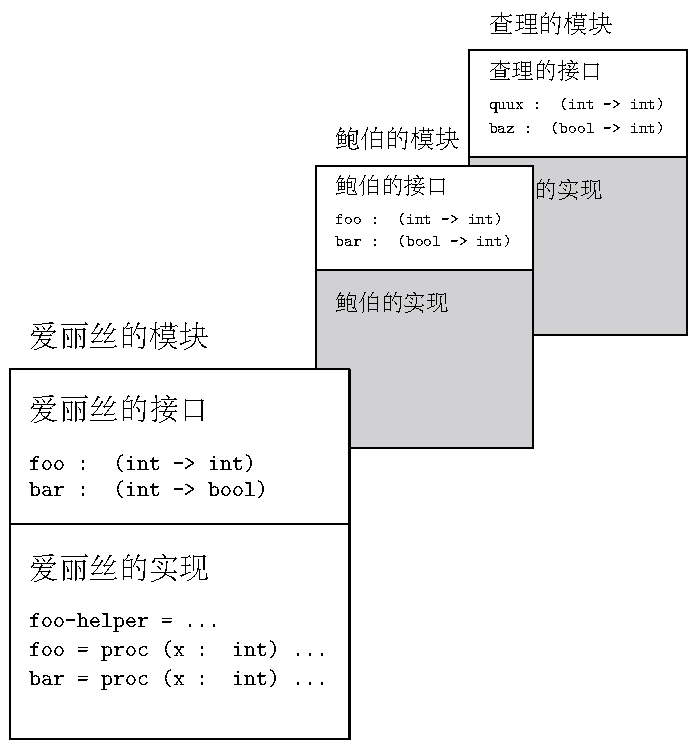
\includegraphics[scale=0.95]{alice-view.pdf}\end{SCentered}

\caption{项目中,爱丽丝所见的三个模块\label{t:x28elem_x22figx2d8x2e1x22x29}}\end{EoplFigure}

\index{zzhu3ti3@主体!mzo2kuai4@模块|idxdecorator{}{}}
\index{szhi2xian4@实现!mzo2kuai4jie1kou3@模块接口|idxdecorator{}{}}
\index{jzie1kou3@接口!mzo2kuai4@模块|idxdecorator{}{}}
这个程序从名为 \Scribtexttt{m1} 的模块定义开始。像任何模块一样,它有\emph{接口}和\Scribtexttt{主体}。
主体\emph{实现}接口。接口\emph{声明}变量 \Scribtexttt{a}、\Scribtexttt{b} 和 \Scribtexttt{c}。主体\emph{定
义}了 \Scribtexttt{a}、\Scribtexttt{x}、\Scribtexttt{b} 和 \Scribtexttt{c} 的绑定。
\index{bzang3ding4Binding@绑定 (Binding)!mzo2kuai4zhong1de@模块中的|idxdecorator{}{}}

当我们求程序的值时,也会求出 \Scribtexttt{m1} 主体中表达式的值。变量 \Scribtexttt{from m1 take a}、
\Scribtexttt{from m1 take b} 和 \Scribtexttt{from m1 take c} 绑定到适当的值,它们的作用域为模块定
义之后。由于 \Scribtexttt{from m1 take x} 未在接口中声明,所以它的作用域不包含模块定义之
后。

\index{szhou4xian4bian4liang4@受限变量|idxdecorator{}{}}
\index{bzian4liang4@变量!szhou4xian4@受限|idxdecorator{}{}}
为了同\emph{简单变量} (\emph{simple variables}) 区别,我们称这些新变量
为\emph{受限变量} (\emph{qualified variables})。在一般的语言中,受限变量可能写作
\Scribtexttt{m1{\hbox{\texttt{.}}}a}、\Scribtexttt{m1{\hbox{\texttt{:}}}a} 或 \Scribtexttt{m1{\hbox{\texttt{:}}}{\hbox{\texttt{:}}}a}。在\ChapRefLocal{t:x28part_x22oacx22x29}{9}{对象和类}探讨的面向对象语言中,
\Scribtexttt{m1{\hbox{\texttt{.}}}a} 通常另有含义。

我们说接口\emph{提出} (\emph{offer})(或称\emph{公布} (\emph{advertise}),
或称\emph{承诺} (\emph{promise}))三个整型值,主体\emph{提
供} (\emph{supply}, \emph{provide})(或称\emph{输出} (\emph{export}))这些值。当模块主体提供的值类型与接口命名变量时公
布的类型相符时,主体\emph{满足}其接口。

\index{letstarzzuo4yong4yu4@\Scribtexttt{let*} 式作用域|idxdecorator{}{}}
在主体中,定义具有 \Scribtexttt{let*} 那样的作用域,所以 \Scribtexttt{x}、\Scribtexttt{b} 和 \Scribtexttt{c} 的定义
在 \Scribtexttt{a} 的作用域内。一些作用域如 所示。

\index{zzhu3ti3@主体!mzo2kuai4cheng2xu4@模块程序|idxdecorator{}{}}
本例中,以 \Scribtexttt{let a = 10} 开头的表达式是\emph{程序主体} (\emph{program body})。它的值
即程序的值。

\index{czhou1xiang4bian1jie4@抽象边界|idxdecorator{}{}}每个模块都在模块主体和程序其余部分之间建立了抽
象边界。模块主体中的表达式在抽象边界\emph{之内},其他部分在抽象边界\emph{之外}。
模块主体也可以提供不在接口中的名字绑定,但那些绑定在程序主体和其他模块中不可见,
正如 所示。在我们的例子中,程序主体不在 \Scribtexttt{from m1 take x}
的作用域内。如果我们写 \Scribtexttt{{-}(from m1 take a, from m1 take x)},程序就会类型异常。

\begin{EoplExample}\label{t:x28elem_x22egx2d8x2e2x22x29}程序

\begin{Subflow}\begin{EoplCodeInset}\begin{SVerbatim}\begin{SingleColumn}\Scribtexttt{module m1}

\Scribtexttt{}\mbox{\hphantom{\Scribtexttt{x}}}\Scribtexttt{interface}

\Scribtexttt{}\mbox{\hphantom{\Scribtexttt{xx}}}\Scribtexttt{[u {\hbox{\texttt{:}}} bool]}

\Scribtexttt{}\mbox{\hphantom{\Scribtexttt{x}}}\Scribtexttt{body}

\Scribtexttt{}\mbox{\hphantom{\Scribtexttt{xx}}}\Scribtexttt{[u = 33]}

\Scribtexttt{}\mbox{\hphantom{\Scribtexttt{x}}}

\Scribtexttt{44}\end{SingleColumn}\end{SVerbatim}\end{EoplCodeInset}

类型异常。即使程序的其他部分不使用那些值,模块主体也要将接口中的名字与适当类型的
值关联起来。\end{Subflow}\end{EoplExample}

\begin{EoplFigure}[!ht]

\noindent \begin{SCentered}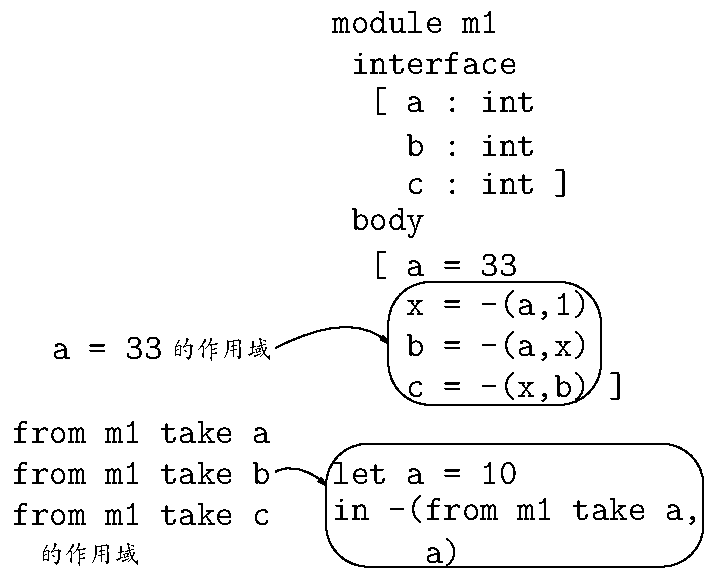
\includegraphics[scale=1.0]{module-contour.pdf}\end{SCentered}

\caption{简单模块中的一些作用域\label{t:x28elem_x22figx2d8x2e2x22x29}}\end{EoplFigure}

\begin{EoplExample}\label{t:x28elem_x22egx2d8x2e3x22x29}模块主体必须提供接口中声明的所有绑定。例如,

\begin{Subflow}\begin{EoplCodeInset}\begin{SVerbatim}\begin{SingleColumn}\Scribtexttt{module m1}

\Scribtexttt{}\mbox{\hphantom{\Scribtexttt{x}}}\Scribtexttt{interface}

\Scribtexttt{}\mbox{\hphantom{\Scribtexttt{xx}}}\Scribtexttt{[u {\hbox{\texttt{:}}} int}

\Scribtexttt{}\mbox{\hphantom{\Scribtexttt{xxx}}}\Scribtexttt{v {\hbox{\texttt{:}}} int]}

\Scribtexttt{}\mbox{\hphantom{\Scribtexttt{x}}}\Scribtexttt{body}

\Scribtexttt{}\mbox{\hphantom{\Scribtexttt{xx}}}\Scribtexttt{[u = 33]}

\Scribtexttt{}\mbox{\hphantom{\Scribtexttt{x}}}

\Scribtexttt{44}\end{SingleColumn}\end{SVerbatim}\end{EoplCodeInset}

类型异常,因为 \Scribtexttt{m1} 的主体没有提供接口中公布的所有值。\end{Subflow}\end{EoplExample}

\begin{EoplExample}\label{t:x28elem_x22egx2d8x2e4x22x29}为了让实现简单一点,我们的语言要求模块主体按照接口声明的顺序给出各值。因此

\begin{Subflow}\begin{EoplCodeInset}\begin{SVerbatim}\begin{SingleColumn}\Scribtexttt{module m1}

\Scribtexttt{}\mbox{\hphantom{\Scribtexttt{x}}}\Scribtexttt{interface}

\Scribtexttt{}\mbox{\hphantom{\Scribtexttt{xx}}}\Scribtexttt{[u {\hbox{\texttt{:}}} int}

\Scribtexttt{}\mbox{\hphantom{\Scribtexttt{xxx}}}\Scribtexttt{v {\hbox{\texttt{:}}} int]}

\Scribtexttt{}\mbox{\hphantom{\Scribtexttt{x}}}\Scribtexttt{body}

\Scribtexttt{}\mbox{\hphantom{\Scribtexttt{xx}}}\Scribtexttt{[v = 33}

\Scribtexttt{}\mbox{\hphantom{\Scribtexttt{xxx}}}\Scribtexttt{u = 44]}

\Scribtexttt{}\mbox{\hphantom{\Scribtexttt{x}}}

\Scribtexttt{from m1 take u}\end{SingleColumn}\end{SVerbatim}\end{EoplCodeInset}

类型异常。可以免除这一限制(ex8.8、ex8.17)。\end{Subflow}\end{EoplExample}

\begin{EoplExample}\label{t:x28elem_x22egx2d8x2e5x22x29}\index{letstarzzuo4yong4yu4@\Scribtexttt{let*} 式作用域|idxdecorator{}{}}
在我们的语言中,模块具有 \Scribtexttt{let*} 式的作用域(ex3.17)。例如,

\begin{Subflow}\begin{EoplCodeInset}\begin{SVerbatim}\begin{SingleColumn}\Scribtexttt{module m1}

\Scribtexttt{}\mbox{\hphantom{\Scribtexttt{x}}}\Scribtexttt{interface}

\Scribtexttt{}\mbox{\hphantom{\Scribtexttt{xx}}}\Scribtexttt{[u {\hbox{\texttt{:}}} int]}

\Scribtexttt{}\mbox{\hphantom{\Scribtexttt{x}}}\Scribtexttt{body}

\Scribtexttt{}\mbox{\hphantom{\Scribtexttt{xx}}}\Scribtexttt{[u = 44]}

\Scribtexttt{}\mbox{\hphantom{\Scribtexttt{x}}}

\Scribtexttt{module m2}

\Scribtexttt{}\mbox{\hphantom{\Scribtexttt{x}}}\Scribtexttt{interface}

\Scribtexttt{}\mbox{\hphantom{\Scribtexttt{xx}}}\Scribtexttt{[v {\hbox{\texttt{:}}} int]}

\Scribtexttt{}\mbox{\hphantom{\Scribtexttt{x}}}\Scribtexttt{body}

\Scribtexttt{}\mbox{\hphantom{\Scribtexttt{xx}}}\Scribtexttt{[v = {-}(from m1 take u,11)]}

\Scribtexttt{}\mbox{\hphantom{\Scribtexttt{x}}}

\Scribtexttt{{-}(from m1 take u, from m2 take v)}\end{SingleColumn}\end{SVerbatim}\end{EoplCodeInset}

类型为 \Scribtexttt{int}。但如果我们交换定义的顺序,

\begin{EoplCodeInset}\begin{SVerbatim}\begin{SingleColumn}\Scribtexttt{module m2}

\Scribtexttt{}\mbox{\hphantom{\Scribtexttt{x}}}\Scribtexttt{interface}

\Scribtexttt{}\mbox{\hphantom{\Scribtexttt{xx}}}\Scribtexttt{[v {\hbox{\texttt{:}}} int]}

\Scribtexttt{}\mbox{\hphantom{\Scribtexttt{x}}}\Scribtexttt{body}

\Scribtexttt{}\mbox{\hphantom{\Scribtexttt{xx}}}\Scribtexttt{[v = {-}(from m1 take u,11)]}

\Scribtexttt{}\mbox{\hphantom{\Scribtexttt{x}}}

\Scribtexttt{module m1}

\Scribtexttt{}\mbox{\hphantom{\Scribtexttt{x}}}\Scribtexttt{interface}

\Scribtexttt{}\mbox{\hphantom{\Scribtexttt{xx}}}\Scribtexttt{[u {\hbox{\texttt{:}}} int]}

\Scribtexttt{}\mbox{\hphantom{\Scribtexttt{x}}}\Scribtexttt{body}

\Scribtexttt{}\mbox{\hphantom{\Scribtexttt{xx}}}\Scribtexttt{[u = 44]}

\Scribtexttt{}\mbox{\hphantom{\Scribtexttt{x}}}

\Scribtexttt{{-}(from m1 take u, from m2 take v)}\end{SingleColumn}\end{SVerbatim}\end{EoplCodeInset}

则类型异常,因为 \Scribtexttt{m2} 主体中使用 \Scribtexttt{from m1 take u} 的地方不在后者的作用域
内。\end{Subflow}\end{EoplExample}

\Ssubsubsection{实现简单模块系统}{实现简单模块系统}\label{t:x28part_x22s8x2e1x2e2x22x29}



\Ssubsubsubsectionstarx{语法}{语法}\label{t:x28part_x22s8x2e1x2dsyntaxx22x29}

SIMPLE{-}MODULES 的程序包含一串模块定义,然后是一个表达式。

\begin{Small}\Iidentity{\begin{align*} \mathit{Program} &::= \{\mathit{ModuleDefn}\}^{*} \mathit{Expression} \\[-3pt]
&\mathrel{\phantom{::=}} \fbox{\Scribtexttt{a{-}program (m{-}defs body)}}\end{align*}}\end{Small}

模块定义包含名字、接口和主体。

\begin{Small}\Iidentity{\begin{align*}\mathit{ModuleDefn} &::= \Scribtexttt{module} \ \mathit{Identifier} \ \Scribtexttt{interface} \ \mathit{Iface} \ \Scribtexttt{body} \ \mathit{ModuleBody} \\[-3pt]
 &\mathrel{\phantom{::=}} \fbox{\Scribtexttt{a{-}module{-}definition (m{-}name expected{-}iface m{-}body)}}\end{align*}}\end{Small}

简单模块的接口包含任意数量的声明。每个声明指定程序中一个变量的类型。
我们称之为\emph{值声明} (\emph{value declaration}),因为要声明的变量表示一个值。在后面
几节中,我们介绍其他类别的接口和声明。

\begin{Small}\Iidentity{\begin{align*}   \mathit{Iface} &::= \Scribtexttt{[} \{\mathit{Decl}\}^{*} \Scribtexttt{]} \\[-3pt]
&\mathrel{\phantom{::=}} \fbox{\Scribtexttt{simple{-}iface (decls)}} \\[-5pt]
    \mathit{Decl} &::= \mathit{Identifier} \Scribtexttt{{\hbox{\texttt{:}}}} \mathit{Type} \\[-3pt]
&\mathrel{\phantom{::=}} \fbox{\Scribtexttt{val{-}decl (var{-}name ty)}}\end{align*}}\end{Small}

模块主体包含任意数量的定义。每个定义将变量和某个表达式的值关联起来。

\begin{Small}\Iidentity{\begin{align*}\mathit{ModuleBody} &::= \Scribtexttt{[} \{\mathit{Defn}\}^{*} \Scribtexttt{]} \\[-3pt]
  &\mathrel{\phantom{::=}} \fbox{\Scribtexttt{defns{-}module{-}body (defns)}} \\[-5pt]
      \mathit{Defn} &::= \mathit{Identifier} \Scribtexttt{=} \mathit{Expression} \\[-3pt]
  &\mathrel{\phantom{::=}} \fbox{\Scribtexttt{val{-}defn (var{-}name exp)}}\end{align*}}\end{Small}

我们的表达式与 CHECKED(\SecRefLocal{t:x28part_x22s7x2e3x22x29}{7.3}{CHECKED:带有类型检查的语言})相同,但我们要修改语法,新增一种表达式,
以便使用受限变量。

\begin{Small}\Iidentity{\begin{align*}\mathit{Expression} &::= \Scribtexttt{from} \mathit{Identifier} \Scribtexttt{take} \mathit{Identifier} \\[-3pt]
  &\mathrel{\phantom{::=}} \fbox{\Scribtexttt{qualified{-}var{-}exp (m{-}name var{-}name)}}\end{align*}}\end{Small}

\Ssubsubsubsectionstarx{解释器}{解释器}\label{t:x28part_x22s8x2e1x2dthex2dinterpreterx22x29}

\index{valueof@\textbf{\Scribtexttt{value{-}of}}!SIMPLEMODULES@SIMPLE{-}MODULES|(idxdecorator{}{}}
求模块主体的值会得到一个\emph{模块}。在我们的简单模块语言中,模块是一个环境,包
含模块输出的所有绑定。我们用数据类型 \Scribtexttt{typed{-}module} 表示这些。

\begin{EoplCodeInset}\begin{SCodeFlow}\begin{RktBlk}\begin{SingleColumn}\RktPn{(}\RktSym{define{-}datatype}\mbox{\hphantom{\Scribtexttt{x}}}\RktSym{typed{-}module}\mbox{\hphantom{\Scribtexttt{x}}}\RktSym{typed{-}module{\hbox{\texttt{?}}}}

\mbox{\hphantom{\Scribtexttt{xx}}}\RktPn{(}\RktSym{simple{-}module}

\mbox{\hphantom{\Scribtexttt{xxxx}}}\RktPn{(}\RktSym{bindings}\mbox{\hphantom{\Scribtexttt{x}}}\RktSym{environment{\hbox{\texttt{?}}}}\RktPn{)}\RktPn{)}\RktPn{)}\end{SingleColumn}\end{RktBlk}\end{SCodeFlow}\end{EoplCodeInset}

我们用一种新的绑定在环境中绑定模块名:

\begin{EoplCodeInset}\begin{SCodeFlow}\begin{RktBlk}\begin{SingleColumn}\RktPn{(}\RktSym{define{-}datatype}\mbox{\hphantom{\Scribtexttt{x}}}\RktSym{environment}\mbox{\hphantom{\Scribtexttt{x}}}\RktSym{environment{\hbox{\texttt{?}}}}

\mbox{\hphantom{\Scribtexttt{xx}}}\RktPn{(}\RktSym{empty{-}env}\RktPn{)}

\mbox{\hphantom{\Scribtexttt{xx}}}\RktPn{(}\RktSym{extend{-}env}\mbox{\hphantom{\Scribtexttt{x}}}\RktSym{{\hbox{\texttt{.}}}{\hbox{\texttt{.}}}{\hbox{\texttt{.}}}as}\mbox{\hphantom{\Scribtexttt{x}}}\RktSym{before{\hbox{\texttt{.}}}{\hbox{\texttt{.}}}{\hbox{\texttt{.}}}}\RktPn{)}

\mbox{\hphantom{\Scribtexttt{xx}}}\RktPn{(}\RktSym{extend{-}env{-}rec}\mbox{\hphantom{\Scribtexttt{x}}}\RktSym{{\hbox{\texttt{.}}}{\hbox{\texttt{.}}}{\hbox{\texttt{.}}}as}\mbox{\hphantom{\Scribtexttt{x}}}\RktSym{before{\hbox{\texttt{.}}}{\hbox{\texttt{.}}}{\hbox{\texttt{.}}}}\RktPn{)}

\mbox{\hphantom{\Scribtexttt{xx}}}\RktPn{(}\RktSym{extend{-}env{-}with{-}module}

\mbox{\hphantom{\Scribtexttt{xxxx}}}\RktPn{(}\RktSym{m{-}name}\mbox{\hphantom{\Scribtexttt{x}}}\RktSym{symbol{\hbox{\texttt{?}}}}\RktPn{)}

\mbox{\hphantom{\Scribtexttt{xxxx}}}\RktPn{(}\RktSym{m{-}val}\mbox{\hphantom{\Scribtexttt{x}}}\RktSym{typed{-}module{\hbox{\texttt{?}}}}\RktPn{)}

\mbox{\hphantom{\Scribtexttt{xxxx}}}\RktPn{(}\RktSym{saved{-}env}\mbox{\hphantom{\Scribtexttt{x}}}\RktSym{environment{\hbox{\texttt{?}}}}\RktPn{)}\RktPn{)}\RktPn{)}\end{SingleColumn}\end{RktBlk}\end{SCodeFlow}\end{EoplCodeInset}

例如,如果我们的程序是

\begin{Subflow}\begin{EoplCodeInset}\begin{SVerbatim}\begin{SingleColumn}\Scribtexttt{module m1}

\Scribtexttt{}\mbox{\hphantom{\Scribtexttt{x}}}\Scribtexttt{interface}

\Scribtexttt{}\mbox{\hphantom{\Scribtexttt{xx}}}\Scribtexttt{[a {\hbox{\texttt{:}}} int}

\Scribtexttt{}\mbox{\hphantom{\Scribtexttt{xxx}}}\Scribtexttt{b {\hbox{\texttt{:}}} int}

\Scribtexttt{}\mbox{\hphantom{\Scribtexttt{xxx}}}\Scribtexttt{c {\hbox{\texttt{:}}} int]}

\Scribtexttt{}\mbox{\hphantom{\Scribtexttt{x}}}\Scribtexttt{body}

\Scribtexttt{}\mbox{\hphantom{\Scribtexttt{xx}}}\Scribtexttt{[a = 33}

\Scribtexttt{}\mbox{\hphantom{\Scribtexttt{xxx}}}\Scribtexttt{b = 44}

\Scribtexttt{}\mbox{\hphantom{\Scribtexttt{xxx}}}\Scribtexttt{c = 55]}

\Scribtexttt{module m2}

\Scribtexttt{}\mbox{\hphantom{\Scribtexttt{x}}}\Scribtexttt{interface}

\Scribtexttt{}\mbox{\hphantom{\Scribtexttt{xx}}}\Scribtexttt{[a {\hbox{\texttt{:}}} int}

\Scribtexttt{}\mbox{\hphantom{\Scribtexttt{xx}}}\Scribtexttt{b {\hbox{\texttt{:}}} int]}

\Scribtexttt{}\mbox{\hphantom{\Scribtexttt{x}}}\Scribtexttt{body}

\Scribtexttt{}\mbox{\hphantom{\Scribtexttt{xx}}}\Scribtexttt{[a = 66}

\Scribtexttt{}\mbox{\hphantom{\Scribtexttt{xxx}}}\Scribtexttt{b = 77]}

\Scribtexttt{let z = 99}

\Scribtexttt{in {-}(z, {-}(from m1 take a, from m2 take a))}\end{SingleColumn}\end{SVerbatim}\end{EoplCodeInset}

那么声明 \texMathInline{z} 之后的环境是

\begin{EoplCodeInset}\begin{SCodeFlow}\begin{RktBlk}\begin{SingleColumn}\RktVal{\#}\RktVal{(}\RktVal{struct{\hbox{\texttt{:}}}extend{-}env}

\mbox{\hphantom{\Scribtexttt{xxx}}}\RktVal{z}\mbox{\hphantom{\Scribtexttt{x}}}\RktVal{\#}\RktVal{(}\RktVal{struct{\hbox{\texttt{:}}}num{-}val}\mbox{\hphantom{\Scribtexttt{x}}}\RktVal{99}\RktVal{)}

\mbox{\hphantom{\Scribtexttt{xxx}}}\RktVal{\#}\RktVal{(}\RktVal{struct{\hbox{\texttt{:}}}extend{-}env{-}with{-}module}

\mbox{\hphantom{\Scribtexttt{xxxxxx}}}\RktVal{m2}\mbox{\hphantom{\Scribtexttt{x}}}\RktVal{\#}\RktVal{(}\RktVal{struct{\hbox{\texttt{:}}}simple{-}module}

\mbox{\hphantom{\Scribtexttt{xxxxxxxxxxxx}}}\RktVal{\#}\RktVal{(}\RktVal{struct{\hbox{\texttt{:}}}extend{-}env}

\mbox{\hphantom{\Scribtexttt{xxxxxxxxxxxxxxx}}}\RktVal{a}\mbox{\hphantom{\Scribtexttt{x}}}\RktVal{\#}\RktVal{(}\RktVal{struct{\hbox{\texttt{:}}}num{-}val}\mbox{\hphantom{\Scribtexttt{x}}}\RktVal{66}\RktVal{)}

\mbox{\hphantom{\Scribtexttt{xxxxxxxxxxxxxxx}}}\RktVal{\#}\RktVal{(}\RktVal{struct{\hbox{\texttt{:}}}extend{-}env}

\mbox{\hphantom{\Scribtexttt{xxxxxxxxxxxxxxxxxx}}}\RktVal{b}\mbox{\hphantom{\Scribtexttt{x}}}\RktVal{\#}\RktVal{(}\RktVal{struct{\hbox{\texttt{:}}}num{-}val}\mbox{\hphantom{\Scribtexttt{x}}}\RktVal{77}\RktVal{)}

\mbox{\hphantom{\Scribtexttt{xxxxxxxxxxxxxxxxxx}}}\RktVal{\#}\RktVal{(}\RktVal{struct{\hbox{\texttt{:}}}empty{-}env}\RktVal{)}\RktVal{)}\RktVal{)}\RktVal{)}

\mbox{\hphantom{\Scribtexttt{xxxxxx}}}\RktVal{\#}\RktVal{(}\RktVal{struct{\hbox{\texttt{:}}}extend{-}env{-}with{-}module}

\mbox{\hphantom{\Scribtexttt{xxxxxxxxx}}}\RktVal{m1}\mbox{\hphantom{\Scribtexttt{x}}}\RktVal{\#}\RktVal{(}\RktVal{struct{\hbox{\texttt{:}}}simple{-}module}

\mbox{\hphantom{\Scribtexttt{xxxxxxxxxxxxxxx}}}\RktVal{\#}\RktVal{(}\RktVal{struct{\hbox{\texttt{:}}}extend{-}env}

\mbox{\hphantom{\Scribtexttt{xxxxxxxxxxxxxxxxxx}}}\RktVal{a}\mbox{\hphantom{\Scribtexttt{x}}}\RktVal{\#}\RktVal{(}\RktVal{struct{\hbox{\texttt{:}}}num{-}val}\mbox{\hphantom{\Scribtexttt{x}}}\RktVal{33}\RktVal{)}

\mbox{\hphantom{\Scribtexttt{xxxxxxxxxxxxxxxxxx}}}\RktVal{\#}\RktVal{(}\RktVal{struct{\hbox{\texttt{:}}}extend{-}env}

\mbox{\hphantom{\Scribtexttt{xxxxxxxxxxxxxxxxxxxxx}}}\RktVal{b}\mbox{\hphantom{\Scribtexttt{x}}}\RktVal{\#}\RktVal{(}\RktVal{struct{\hbox{\texttt{:}}}num{-}val}\mbox{\hphantom{\Scribtexttt{x}}}\RktVal{44}\RktVal{)}

\mbox{\hphantom{\Scribtexttt{xxxxxxxxxxxxxxxxxxxxx}}}\RktVal{\#}\RktVal{(}\RktVal{struct{\hbox{\texttt{:}}}extend{-}env}

\mbox{\hphantom{\Scribtexttt{xxxxxxxxxxxxxxxxxxxxxxxx}}}\RktVal{c}\mbox{\hphantom{\Scribtexttt{x}}}\RktVal{\#}\RktVal{(}\RktVal{struct{\hbox{\texttt{:}}}num{-}val}\mbox{\hphantom{\Scribtexttt{x}}}\RktVal{55}\RktVal{)}

\mbox{\hphantom{\Scribtexttt{xxxxxxxxxxxxxxxxxxxxxxxx}}}\RktVal{\#}\RktVal{(}\RktVal{struct{\hbox{\texttt{:}}}empty{-}env}\RktVal{)}\RktVal{)}\RktVal{)}\RktVal{)}\RktVal{)}

\mbox{\hphantom{\Scribtexttt{xxxxxxxxx}}}\RktVal{\#}\RktVal{(}\RktVal{struct{\hbox{\texttt{:}}}empty{-}env}\RktVal{)}\RktVal{)}\RktVal{)}\RktVal{)}\end{SingleColumn}\end{RktBlk}\end{SCodeFlow}\end{EoplCodeInset}

在这个环境中,\Scribtexttt{m1} 和 \Scribtexttt{m2} 各绑定到一个简单模块,二者分别包含一个小环境。\end{Subflow}

\index{szhou4xian4bian4liang4@受限变量|idxdecorator{}{}}
我们用 \Scribtexttt{lookup{-}qualified{-}var{-}in{-}env} 求受限变量 \Scribtexttt{from }\texMathInline{m}\Scribtexttt{ take }\texMathInline{var}
引用的值。它在当前环境中查找模块 \texMathInline{m},然后在得到的环境中查找 \texMathInline{var}。

\begin{EoplCodeInset}\begin{SCodeFlow}\begin{RktBlk}\begin{SingleColumn}\textbf{\Scribtexttt{lookup{-}qualified{-}var{-}in{-}env{\hbox{\texttt{!}}}}} : \texMathInline{\mathit{Sym} \times \mathit{Sym} \times \mathit{Env} \to \mathit{ExpVal}}

\RktPn{(}\RktSym{define}\mbox{\hphantom{\Scribtexttt{x}}}\RktSym{lookup{-}qualified{-}var{-}in{-}env}

\mbox{\hphantom{\Scribtexttt{xx}}}\RktPn{(}\RktSym{lambda}\mbox{\hphantom{\Scribtexttt{x}}}\RktPn{(}\RktSym{m{-}name}\mbox{\hphantom{\Scribtexttt{x}}}\RktSym{var{-}name}\mbox{\hphantom{\Scribtexttt{x}}}\RktSym{env}\RktPn{)}

\mbox{\hphantom{\Scribtexttt{xxxx}}}\RktPn{(}\RktSym{let}\mbox{\hphantom{\Scribtexttt{x}}}\RktPn{(}\RktPn{(}\RktSym{m{-}val}\mbox{\hphantom{\Scribtexttt{x}}}\RktPn{(}\RktSym{lookup{-}module{-}name{-}in{-}env}\mbox{\hphantom{\Scribtexttt{x}}}\RktSym{m{-}name}\mbox{\hphantom{\Scribtexttt{x}}}\RktSym{env}\RktPn{)}\RktPn{)}\RktPn{)}

\mbox{\hphantom{\Scribtexttt{xxxxxx}}}\RktPn{(}\RktSym{cases}\mbox{\hphantom{\Scribtexttt{x}}}\RktSym{typed{-}module}\mbox{\hphantom{\Scribtexttt{x}}}\RktSym{m{-}val}

\mbox{\hphantom{\Scribtexttt{xxxxxxxx}}}\RktPn{(}\RktSym{simple{-}module}\mbox{\hphantom{\Scribtexttt{x}}}\RktPn{(}\RktSym{bindings}\RktPn{)}

\mbox{\hphantom{\Scribtexttt{xxxxxxxxxx}}}\RktPn{(}\RktSym{apply{-}env}\mbox{\hphantom{\Scribtexttt{x}}}\RktSym{bindings}\mbox{\hphantom{\Scribtexttt{x}}}\RktSym{var{-}name}\RktPn{)}\RktPn{)}\RktPn{)}\RktPn{)}\RktPn{)}\RktPn{)}\end{SingleColumn}\end{RktBlk}\end{SCodeFlow}\end{EoplCodeInset}

要求程序的值,我们把所有模块定义加入当前环境中,得到初始环境,然后求程序主体的值。
过程 \Scribtexttt{add{-}module{-}defns{-}to{-}env} 遍历模块定义,求每个模块定义主体的值,并将得到
的模块加入当前环境中,如 所示。

\index{zzhu3ti3@主体!mzo2kuai4@模块|idxdecorator{}{}}
\index{letstarzzuo4yong4yu4@\Scribtexttt{let*} 式作用域|idxdecorator{}{}}
最后,要求模块主体的值,我们按照 \Scribtexttt{let*} 式定界,在适当的环境内求每个表达式的
值,得出一环境。过程 \Scribtexttt{defns{-}to{-}env} 生成的环境只包含定义 \Scribtexttt{defns} 产生的绑
定()。
\index{valueof@\textbf{\Scribtexttt{value{-}of}}!SIMPLEMODULES@SIMPLE{-}MODULES|)idxdecorator{}{}}

\begin{EoplFigure}[!t]

\begin{SCodeFlow}\begin{RktBlk}\begin{SingleColumn}\textbf{\Scribtexttt{value{-}of{-}program}} : \texMathInline{\mathit{Program} \to \mathit{ExpVal}}

\RktPn{(}\RktSym{define}\mbox{\hphantom{\Scribtexttt{x}}}\RktSym{value{-}of{-}program}

\mbox{\hphantom{\Scribtexttt{xx}}}\RktPn{(}\RktSym{lambda}\mbox{\hphantom{\Scribtexttt{x}}}\RktPn{(}\RktSym{pgm}\RktPn{)}

\mbox{\hphantom{\Scribtexttt{xxxx}}}\RktPn{(}\RktSym{cases}\mbox{\hphantom{\Scribtexttt{x}}}\RktSym{program}\mbox{\hphantom{\Scribtexttt{x}}}\RktSym{pgm}

\mbox{\hphantom{\Scribtexttt{xxxxxx}}}\RktPn{(}\RktSym{a{-}program}\mbox{\hphantom{\Scribtexttt{x}}}\RktPn{(}\RktSym{m{-}defns}\mbox{\hphantom{\Scribtexttt{x}}}\RktSym{body}\RktPn{)}

\mbox{\hphantom{\Scribtexttt{xxxxxxxx}}}\RktPn{(}\RktSym{value{-}of}\mbox{\hphantom{\Scribtexttt{x}}}\RktSym{body}

\mbox{\hphantom{\Scribtexttt{xxxxxxxxxx}}}\RktPn{(}\RktSym{add{-}module{-}defns{-}to{-}env}\mbox{\hphantom{\Scribtexttt{x}}}\RktSym{m{-}defns}\mbox{\hphantom{\Scribtexttt{x}}}\RktPn{(}\RktSym{empty{-}env}\RktPn{)}\RktPn{)}\RktPn{)}\RktPn{)}\RktPn{)}\RktPn{)}\RktPn{)}

\mbox{\hphantom{\Scribtexttt{x}}}

\textbf{\Scribtexttt{add{-}module{-}defns{-}to{-}env}} : \texMathInline{\mathit{Listof(Defn)} \times \mathit{Env} \to \mathit{Env}}

\RktPn{(}\RktSym{define}\mbox{\hphantom{\Scribtexttt{x}}}\RktSym{add{-}module{-}defns{-}to{-}env}

\mbox{\hphantom{\Scribtexttt{xx}}}\RktPn{(}\RktSym{lambda}\mbox{\hphantom{\Scribtexttt{x}}}\RktPn{(}\RktSym{defns}\mbox{\hphantom{\Scribtexttt{x}}}\RktSym{env}\RktPn{)}

\mbox{\hphantom{\Scribtexttt{xxxx}}}\RktPn{(}\RktSym{if}\mbox{\hphantom{\Scribtexttt{x}}}\RktPn{(}\RktSym{null{\hbox{\texttt{?}}}}\mbox{\hphantom{\Scribtexttt{x}}}\RktSym{defns}\RktPn{)}

\mbox{\hphantom{\Scribtexttt{xxxxxx}}}\RktSym{env}

\mbox{\hphantom{\Scribtexttt{xxxxxx}}}\RktPn{(}\RktSym{cases}\mbox{\hphantom{\Scribtexttt{x}}}\RktSym{module{-}definition}\mbox{\hphantom{\Scribtexttt{x}}}\RktPn{(}\RktSym{car}\mbox{\hphantom{\Scribtexttt{x}}}\RktSym{defns}\RktPn{)}

\mbox{\hphantom{\Scribtexttt{xxxxxxxx}}}\RktPn{(}\RktSym{a{-}module{-}definition}\mbox{\hphantom{\Scribtexttt{x}}}\RktPn{(}\RktSym{m{-}name}\mbox{\hphantom{\Scribtexttt{x}}}\RktSym{iface}\mbox{\hphantom{\Scribtexttt{x}}}\RktSym{m{-}body}\RktPn{)}

\mbox{\hphantom{\Scribtexttt{xxxxxxxxxx}}}\RktPn{(}\RktSym{add{-}module{-}defns{-}to{-}env}

\mbox{\hphantom{\Scribtexttt{xxxxxxxxxxxx}}}\RktPn{(}\RktSym{cdr}\mbox{\hphantom{\Scribtexttt{x}}}\RktSym{defns}\RktPn{)}

\mbox{\hphantom{\Scribtexttt{xxxxxxxxxxxx}}}\RktPn{(}\RktSym{extend{-}env{-}with{-}module}

\mbox{\hphantom{\Scribtexttt{xxxxxxxxxxxxxx}}}\RktSym{m{-}name}

\mbox{\hphantom{\Scribtexttt{xxxxxxxxxxxxxx}}}\RktPn{(}\RktSym{value{-}of{-}module{-}body}\mbox{\hphantom{\Scribtexttt{x}}}\RktSym{m{-}body}\mbox{\hphantom{\Scribtexttt{x}}}\RktSym{env}\RktPn{)}

\mbox{\hphantom{\Scribtexttt{xxxxxxxxxxxxxx}}}\RktSym{env}\RktPn{)}\RktPn{)}\RktPn{)}\RktPn{)}\RktPn{)}\RktPn{)}\RktPn{)}\end{SingleColumn}\end{RktBlk}\end{SCodeFlow}

\caption{SIMPLE{-}MODULES 的解释器,第 1 部分\label{t:x28elem_x22figx2d8x2e3x22x29}}

\noindent \index{valueof@\textbf{\Scribtexttt{value{-}of}}!SIMPLEMODULES@SIMPLE{-}MODULES|idxdecorator{}{}}\end{EoplFigure}

\begin{EoplFigure}[!ht]

\begin{SCodeFlow}\begin{RktBlk}\begin{SingleColumn}\textbf{\Scribtexttt{value{-}of{-}module{-}body}} : \texMathInline{\mathit{ModuleBody} \times \mathit{Env} \to \mathit{TypedModule}}

\RktPn{(}\RktSym{define}\mbox{\hphantom{\Scribtexttt{x}}}\RktSym{value{-}of{-}module{-}body}

\mbox{\hphantom{\Scribtexttt{xx}}}\RktPn{(}\RktSym{lambda}\mbox{\hphantom{\Scribtexttt{x}}}\RktPn{(}\RktSym{m{-}body}\mbox{\hphantom{\Scribtexttt{x}}}\RktSym{env}\RktPn{)}

\mbox{\hphantom{\Scribtexttt{xxxx}}}\RktPn{(}\RktSym{cases}\mbox{\hphantom{\Scribtexttt{x}}}\RktSym{module{-}body}\mbox{\hphantom{\Scribtexttt{x}}}\RktSym{m{-}body}

\mbox{\hphantom{\Scribtexttt{xxxxxx}}}\RktPn{(}\RktSym{defns{-}module{-}body}\mbox{\hphantom{\Scribtexttt{x}}}\RktPn{(}\RktSym{defns}\RktPn{)}

\mbox{\hphantom{\Scribtexttt{xxxxxxxx}}}\RktPn{(}\RktSym{simple{-}module}

\mbox{\hphantom{\Scribtexttt{xxxxxxxxxx}}}\RktPn{(}\RktSym{defns{-}to{-}env}\mbox{\hphantom{\Scribtexttt{x}}}\RktSym{defns}\mbox{\hphantom{\Scribtexttt{x}}}\RktSym{env}\RktPn{)}\RktPn{)}\RktPn{)}\RktPn{)}\RktPn{)}\RktPn{)}

\mbox{\hphantom{\Scribtexttt{x}}}

\textbf{\Scribtexttt{defns{-}to{-}env}} : \texMathInline{\mathit{Listof(Defn)} \times \mathit{Env} \to \mathit{Env}}

\RktPn{(}\RktSym{define}\mbox{\hphantom{\Scribtexttt{x}}}\RktSym{defns{-}to{-}env}

\mbox{\hphantom{\Scribtexttt{xx}}}\RktPn{(}\RktSym{lambda}\mbox{\hphantom{\Scribtexttt{x}}}\RktPn{(}\RktSym{defns}\mbox{\hphantom{\Scribtexttt{x}}}\RktSym{env}\RktPn{)}

\mbox{\hphantom{\Scribtexttt{xxxx}}}\RktPn{(}\RktSym{if}\mbox{\hphantom{\Scribtexttt{x}}}\RktPn{(}\RktSym{null{\hbox{\texttt{?}}}}\mbox{\hphantom{\Scribtexttt{x}}}\RktSym{defns}\RktPn{)}

\mbox{\hphantom{\Scribtexttt{xxxxxx}}}\RktPn{(}\RktSym{empty{-}env}\RktPn{)}

\mbox{\hphantom{\Scribtexttt{xxxxxx}}}\RktPn{(}\RktSym{cases}\mbox{\hphantom{\Scribtexttt{x}}}\RktSym{definition}\mbox{\hphantom{\Scribtexttt{x}}}\RktPn{(}\RktSym{car}\mbox{\hphantom{\Scribtexttt{x}}}\RktSym{defns}\RktPn{)}

\mbox{\hphantom{\Scribtexttt{xxxxxxxx}}}\RktPn{(}\RktSym{val{-}defn}\mbox{\hphantom{\Scribtexttt{x}}}\RktPn{(}\RktSym{var}\mbox{\hphantom{\Scribtexttt{x}}}\RktSym{exp}\RktPn{)}

\mbox{\hphantom{\Scribtexttt{xxxxxxxxxx}}}\RktPn{(}\RktSym{let}\mbox{\hphantom{\Scribtexttt{x}}}\RktPn{(}\RktPn{(}\RktSym{val}\mbox{\hphantom{\Scribtexttt{x}}}\RktPn{(}\RktSym{value{-}of}\mbox{\hphantom{\Scribtexttt{x}}}\RktSym{exp}\mbox{\hphantom{\Scribtexttt{x}}}\RktSym{env}\RktPn{)}\RktPn{)}\RktPn{)}

\mbox{\hphantom{\Scribtexttt{xxxxxxxxxxxx}}}\RktPn{(}\RktSym{let}\mbox{\hphantom{\Scribtexttt{x}}}\RktPn{(}\RktPn{(}\RktSym{new{-}env}\mbox{\hphantom{\Scribtexttt{x}}}\RktPn{(}\RktSym{extend{-}env}\mbox{\hphantom{\Scribtexttt{x}}}\RktSym{var}\mbox{\hphantom{\Scribtexttt{x}}}\RktSym{val}\mbox{\hphantom{\Scribtexttt{x}}}\RktSym{env}\RktPn{)}\RktPn{)}\RktPn{)}

\mbox{\hphantom{\Scribtexttt{xxxxxxxxxxxxxx}}}\RktPn{(}\RktSym{extend{-}env}\mbox{\hphantom{\Scribtexttt{x}}}\RktSym{var}\mbox{\hphantom{\Scribtexttt{x}}}\RktSym{val}

\mbox{\hphantom{\Scribtexttt{xxxxxxxxxxxxxxxx}}}\RktPn{(}\RktSym{defns{-}to{-}env}

\mbox{\hphantom{\Scribtexttt{xxxxxxxxxxxxxxxxxx}}}\RktPn{(}\RktSym{cdr}\mbox{\hphantom{\Scribtexttt{x}}}\RktSym{defns}\RktPn{)}\mbox{\hphantom{\Scribtexttt{x}}}\RktSym{new{-}env}\RktPn{)}\RktPn{)}\RktPn{)}\RktPn{)}\RktPn{)}\RktPn{)}\RktPn{)}\RktPn{)}\RktPn{)}\end{SingleColumn}\end{RktBlk}\end{SCodeFlow}

\caption{SIMPLE{-}MODULES 的解释器,第 2 部分\label{t:x28elem_x22figx2d8x2e4x22x29}}

\noindent \index{valueof@\textbf{\Scribtexttt{value{-}of}}!SIMPLEMODULES@SIMPLE{-}MODULES|idxdecorator{}{}}\end{EoplFigure}

\Ssubsubsubsectionstarx{检查器}{检查器}\label{t:x28part_x22s8x2e1x2dcheckerx22x29}

\index{lzei4xing2jian3cha2@类型检查!mzo2kuai4@模块|(idxdecorator{}{}}
检查器的工作是确保所有模块主体满足其接口,且所有变量的使用符合其类型。

\index{letstarzzuo4yong4yu4@\Scribtexttt{let*} 式作用域|idxdecorator{}{}}
我们语言的定界规则很简单:模块遵循 \Scribtexttt{let*} 式定界,依次进入模块输出绑定中的受
限变量的作用域。接口告诉我们每个受限变量的类型。声明和定义也都遵循 \Scribtexttt{let*} 式
定界(如)。

就像\ChapRefLocal{t:x28part_x22typesx22x29}{7}{类型}中的检查器那样,我们用类型环境记录与当前作用域内各名字的相关信
息。因为我们现在有了模块名,我们要在类型环境中绑定模块名。每个模块名绑定到模块的
接口,作为其类型。

\begin{EoplCodeInset}\begin{SCodeFlow}\begin{RktBlk}\begin{SingleColumn}\RktPn{(}\RktSym{define{-}datatype}\mbox{\hphantom{\Scribtexttt{x}}}\RktSym{type{-}environment}\mbox{\hphantom{\Scribtexttt{x}}}\RktSym{type{-}environment{\hbox{\texttt{?}}}}

\mbox{\hphantom{\Scribtexttt{xx}}}\RktPn{(}\RktSym{empty{-}tenv}\RktPn{)}

\mbox{\hphantom{\Scribtexttt{xx}}}\RktPn{(}\RktSym{extend{-}tenv}\mbox{\hphantom{\Scribtexttt{x}}}\emph{...同前...}\RktPn{)}

\mbox{\hphantom{\Scribtexttt{xx}}}\RktPn{(}\RktSym{extend{-}tenv{-}with{-}module}

\mbox{\hphantom{\Scribtexttt{xxxx}}}\RktPn{(}\RktSym{name}\mbox{\hphantom{\Scribtexttt{x}}}\RktSym{symbol{\hbox{\texttt{?}}}}\RktPn{)}

\mbox{\hphantom{\Scribtexttt{xxxx}}}\RktPn{(}\RktSym{interface}\mbox{\hphantom{\Scribtexttt{x}}}\RktSym{interface{\hbox{\texttt{?}}}}\RktPn{)}

\mbox{\hphantom{\Scribtexttt{xxxx}}}\RktPn{(}\RktSym{saved{-}tenv}\mbox{\hphantom{\Scribtexttt{x}}}\RktSym{type{-}environment{\hbox{\texttt{?}}}}\RktPn{)}\RktPn{)}\RktPn{)}\end{SingleColumn}\end{RktBlk}\end{SCodeFlow}\end{EoplCodeInset}

要找出受限变量 \Scribtexttt{from }\texMathInline{m}\Scribtexttt{ take }\texMathInline{var} 的类型,我们首先在类型环境中找出
\texMathInline{m},然后在得到的接口中查找 \texMathInline{var} 的类型。

\begin{EoplCodeInset}\begin{SCodeFlow}\begin{RktBlk}\begin{SingleColumn}\textbf{\Scribtexttt{lookup{-}qualified{-}var{-}in{-}tenv}} : \texMathInline{\mathit{Sym} \times \mathit{Sym} \times \mathit{Tenv} \to \mathit{Type}}

\RktPn{(}\RktSym{define}\mbox{\hphantom{\Scribtexttt{x}}}\RktSym{lookup{-}qualified{-}var{-}in{-}tenv}

\mbox{\hphantom{\Scribtexttt{xx}}}\RktPn{(}\RktSym{lambda}\mbox{\hphantom{\Scribtexttt{x}}}\RktPn{(}\RktSym{m{-}name}\mbox{\hphantom{\Scribtexttt{x}}}\RktSym{var{-}name}\mbox{\hphantom{\Scribtexttt{x}}}\RktSym{tenv}\RktPn{)}

\mbox{\hphantom{\Scribtexttt{xxxx}}}\RktPn{(}\RktSym{let}\mbox{\hphantom{\Scribtexttt{x}}}\RktPn{(}\RktPn{(}\RktSym{iface}\mbox{\hphantom{\Scribtexttt{x}}}\RktPn{(}\RktSym{lookup{-}module{-}name{-}in{-}tenv}\mbox{\hphantom{\Scribtexttt{x}}}\RktSym{tenv}\mbox{\hphantom{\Scribtexttt{x}}}\RktSym{m{-}name}\RktPn{)}\RktPn{)}\RktPn{)}

\mbox{\hphantom{\Scribtexttt{xxxxxx}}}\RktPn{(}\RktSym{cases}\mbox{\hphantom{\Scribtexttt{x}}}\RktSym{interface}\mbox{\hphantom{\Scribtexttt{x}}}\RktSym{iface}

\mbox{\hphantom{\Scribtexttt{xxxxxxxx}}}\RktPn{(}\RktSym{simple{-}iface}\mbox{\hphantom{\Scribtexttt{x}}}\RktPn{(}\RktSym{decls}\RktPn{)}

\mbox{\hphantom{\Scribtexttt{xxxxxxxxxx}}}\RktPn{(}\RktSym{lookup{-}variable{-}name{-}in{-}decls}\mbox{\hphantom{\Scribtexttt{x}}}\RktSym{var{-}name}\mbox{\hphantom{\Scribtexttt{x}}}\RktSym{decls}\RktPn{)}\RktPn{)}\RktPn{)}\RktPn{)}\RktPn{)}\RktPn{)}\end{SingleColumn}\end{RktBlk}\end{SCodeFlow}\end{EoplCodeInset}

\begin{EoplFigure}[!t]

\begin{SCodeFlow}\begin{RktBlk}\begin{SingleColumn}\textbf{\Scribtexttt{type{-}of{-}program}} : \texMathInline{\mathit{Program} \to \mathit{Type}}

\RktPn{(}\RktSym{define}\mbox{\hphantom{\Scribtexttt{x}}}\RktSym{type{-}of{-}program}

\mbox{\hphantom{\Scribtexttt{xx}}}\RktPn{(}\RktSym{lambda}\mbox{\hphantom{\Scribtexttt{x}}}\RktPn{(}\RktSym{pgm}\RktPn{)}

\mbox{\hphantom{\Scribtexttt{xxxx}}}\RktPn{(}\RktSym{cases}\mbox{\hphantom{\Scribtexttt{x}}}\RktSym{program}\mbox{\hphantom{\Scribtexttt{x}}}\RktSym{pgm}

\mbox{\hphantom{\Scribtexttt{xxxxxx}}}\RktPn{(}\RktSym{a{-}program}\mbox{\hphantom{\Scribtexttt{x}}}\RktPn{(}\RktSym{module{-}defns}\mbox{\hphantom{\Scribtexttt{x}}}\RktSym{body}\RktPn{)}

\mbox{\hphantom{\Scribtexttt{xxxxxxxx}}}\RktPn{(}\RktSym{type{-}of}\mbox{\hphantom{\Scribtexttt{x}}}\RktSym{body}

\mbox{\hphantom{\Scribtexttt{xxxxxxxxxx}}}\RktPn{(}\RktSym{add{-}module{-}defns{-}to{-}tenv}\mbox{\hphantom{\Scribtexttt{x}}}\RktSym{module{-}defns}

\mbox{\hphantom{\Scribtexttt{xxxxxxxxxxxx}}}\RktPn{(}\RktSym{empty{-}tenv}\RktPn{)}\RktPn{)}\RktPn{)}\RktPn{)}\RktPn{)}\RktPn{)}\RktPn{)}

\mbox{\hphantom{\Scribtexttt{x}}}

\textbf{\Scribtexttt{add{-}module{-}defns{-}to{-}tenv}} : \texMathInline{\mathit{Listof(ModuleDefn)} \times \mathit{Tenv} \to \mathit{Tenv}}

\RktPn{(}\RktSym{define}\mbox{\hphantom{\Scribtexttt{x}}}\RktSym{add{-}module{-}defns{-}to{-}tenv}

\mbox{\hphantom{\Scribtexttt{xx}}}\RktPn{(}\RktSym{lambda}\mbox{\hphantom{\Scribtexttt{x}}}\RktPn{(}\RktSym{defns}\mbox{\hphantom{\Scribtexttt{x}}}\RktSym{tenv}\RktPn{)}

\mbox{\hphantom{\Scribtexttt{xxxx}}}\RktPn{(}\RktSym{if}\mbox{\hphantom{\Scribtexttt{x}}}\RktPn{(}\RktSym{null{\hbox{\texttt{?}}}}\mbox{\hphantom{\Scribtexttt{x}}}\RktSym{defns}\RktPn{)}

\mbox{\hphantom{\Scribtexttt{xxxxxx}}}\RktSym{tenv}

\mbox{\hphantom{\Scribtexttt{xxxxxx}}}\RktPn{(}\RktSym{cases}\mbox{\hphantom{\Scribtexttt{x}}}\RktSym{module{-}definition}\mbox{\hphantom{\Scribtexttt{x}}}\RktPn{(}\RktSym{car}\mbox{\hphantom{\Scribtexttt{x}}}\RktSym{defns}\RktPn{)}

\mbox{\hphantom{\Scribtexttt{xxxxxxxx}}}\RktPn{(}\RktSym{a{-}module{-}definition}\mbox{\hphantom{\Scribtexttt{x}}}\RktPn{(}\RktSym{m{-}name}\mbox{\hphantom{\Scribtexttt{x}}}\RktSym{expected{-}iface}\mbox{\hphantom{\Scribtexttt{x}}}\RktSym{m{-}body}\RktPn{)}

\mbox{\hphantom{\Scribtexttt{xxxxxxxxxx}}}\RktPn{(}\RktSym{let}\mbox{\hphantom{\Scribtexttt{x}}}\RktPn{(}\RktPn{(}\RktSym{actual{-}iface}\mbox{\hphantom{\Scribtexttt{x}}}\RktPn{(}\RktSym{interface{-}of}\mbox{\hphantom{\Scribtexttt{x}}}\RktSym{m{-}body}\mbox{\hphantom{\Scribtexttt{x}}}\RktSym{tenv}\RktPn{)}\RktPn{)}\RktPn{)}

\mbox{\hphantom{\Scribtexttt{xxxxxxxxxxxx}}}\RktPn{(}\RktSym{if}\mbox{\hphantom{\Scribtexttt{x}}}\RktPn{(}\RktSym{{\Stttextless}{\hbox{\texttt{:}}}{-}iface}\mbox{\hphantom{\Scribtexttt{x}}}\RktSym{actual{-}iface}\mbox{\hphantom{\Scribtexttt{x}}}\RktSym{expected{-}iface}\mbox{\hphantom{\Scribtexttt{x}}}\RktSym{tenv}\RktPn{)}

\mbox{\hphantom{\Scribtexttt{xxxxxxxxxxxxxx}}}\RktPn{(}\RktSym{let}\mbox{\hphantom{\Scribtexttt{x}}}\RktPn{(}\RktPn{(}\RktSym{new{-}tenv}

\mbox{\hphantom{\Scribtexttt{xxxxxxxxxxxxxxxxxxxxxx}}}\RktPn{(}\RktSym{extend{-}tenv{-}with{-}module}

\mbox{\hphantom{\Scribtexttt{xxxxxxxxxxxxxxxxxxxxxxxx}}}\RktSym{m{-}name}

\mbox{\hphantom{\Scribtexttt{xxxxxxxxxxxxxxxxxxxxxxxx}}}\RktSym{expected{-}iface}

\mbox{\hphantom{\Scribtexttt{xxxxxxxxxxxxxxxxxxxxxxxx}}}\RktSym{tenv}\RktPn{)}\RktPn{)}\RktPn{)}

\mbox{\hphantom{\Scribtexttt{xxxxxxxxxxxxxxxx}}}\RktPn{(}\RktSym{add{-}module{-}defns{-}to{-}tenv}

\mbox{\hphantom{\Scribtexttt{xxxxxxxxxxxxxxxxxx}}}\RktPn{(}\RktSym{cdr}\mbox{\hphantom{\Scribtexttt{x}}}\RktSym{defns}\RktPn{)}\mbox{\hphantom{\Scribtexttt{x}}}\RktSym{new{-}tenv}\RktPn{)}\RktPn{)}

\mbox{\hphantom{\Scribtexttt{xxxxxxxxxxxxxx}}}\RktPn{(}\RktSym{report{-}module{-}doesnt{-}satisfy{-}iface}

\mbox{\hphantom{\Scribtexttt{xxxxxxxxxxxxxxxx}}}\RktSym{m{-}name}\mbox{\hphantom{\Scribtexttt{x}}}\RktSym{expected{-}iface}\mbox{\hphantom{\Scribtexttt{x}}}\RktSym{actual{-}iface}\RktPn{)}\RktPn{)}\RktPn{)}\RktPn{)}\RktPn{)}\RktPn{)}\RktPn{)}\RktPn{)}\end{SingleColumn}\end{RktBlk}\end{SCodeFlow}

\caption{SIMPLE{-}MODULES 的检查器,第 1 部分\label{t:x28elem_x22figx2d8x2e5x22x29}}\end{EoplFigure}

就像\ChapRefLocal{t:x28part_x22typesx22x29}{7}{类型}那样,对程序做类型检查的过程类模仿程序的求值,但我们记录的不是
值,而是类型。我们用 \Scribtexttt{type{-}of{-}program} 代替 \Scribtexttt{value{-}of{-}program},用
\Scribtexttt{add{-}module{-}defns{-}to{-}tenv} 代替 \Scribtexttt{add{-}module{-}defns{-}to{-}env}。过程
\Scribtexttt{add{-}module{-}defns{-}to{-}tenv} 用 \Scribtexttt{{\Stttextless}{\hbox{\texttt{:}}}{-}iface} 检查各模块主体产生的接口与提出的
接口是否相符;如果相符,就将模块加入到类型环境中;否则报错。

\index{lzei4xing2jie2gou4@类型结构!mzo2kuai4jie1kou3@模块接口|(idxdecorator{}{}}
模块主体的接口将主体中定义的各个变量与定义中的类型关联起来。例如,如果我们查看第
一个例子的主体,

\begin{Subflow}\begin{EoplCodeInset}\begin{SVerbatim}\begin{SingleColumn}\Scribtexttt{[a = 33}

\Scribtexttt{}\mbox{\hphantom{\Scribtexttt{x}}}\Scribtexttt{x = {-}(a,1)}

\Scribtexttt{}\mbox{\hphantom{\Scribtexttt{x}}}\Scribtexttt{b = {-}(a,x)}

\Scribtexttt{}\mbox{\hphantom{\Scribtexttt{x}}}\Scribtexttt{c = {-}(x,b)]}\end{SingleColumn}\end{SVerbatim}\end{EoplCodeInset}

可得

\begin{EoplCodeInset}\begin{SVerbatim}\begin{SingleColumn}\Scribtexttt{[a {\hbox{\texttt{:}}} int}

\Scribtexttt{}\mbox{\hphantom{\Scribtexttt{x}}}\Scribtexttt{x {\hbox{\texttt{:}}} int}

\Scribtexttt{}\mbox{\hphantom{\Scribtexttt{x}}}\Scribtexttt{b {\hbox{\texttt{:}}} int}

\Scribtexttt{}\mbox{\hphantom{\Scribtexttt{x}}}\Scribtexttt{c {\hbox{\texttt{:}}} int]}\end{SingleColumn}\end{SVerbatim}\end{EoplCodeInset}\end{Subflow}

一旦我们建立了一套接口来描述模块主体输出的所有绑定,我们就能将其与模块公布的接口
比较。

回忆一下,简单接口包含一个声明列表。过程 \Scribtexttt{defns{-}to{-}decls} 创建这样的列表,调
用 \Scribtexttt{type{-}of} 找出每个定义的类型。在每一步,它还按 \Scribtexttt{let*} 定界,扩展局部类
型环境(见)。

剩下的只是用 \Scribtexttt{{\Stttextless}{\hbox{\texttt{:}}}{-}iface} 比较每个模块的期望类型与实际类型。我们将 \Scribtexttt{{\Stttextless}{\hbox{\texttt{:}}}} 定义
为:若 \texMathInline{i_1 \Scribtexttt{{\Stttextless}{\hbox{\texttt{:}}}} i_2},则满足接口 \texMathInline{i_1} 的任何模块也满足接口 \texMathInline{i_2}。例如

\begin{Subflow}\begin{EoplCodeInset}\begin{SVerbatim}\begin{SingleColumn}\Scribtexttt{[u {\hbox{\texttt{:}}} int}\mbox{\hphantom{\Scribtexttt{xxxxxxxxx}}}\Scribtexttt{[u {\hbox{\texttt{:}}} int}

\Scribtexttt{}\mbox{\hphantom{\Scribtexttt{x}}}\Scribtexttt{v {\hbox{\texttt{:}}} int}\mbox{\hphantom{\Scribtexttt{xxxx}}}\Scribtexttt{{\Stttextless}{\hbox{\texttt{:}}}}\mbox{\hphantom{\Scribtexttt{xxxx}}}\Scribtexttt{z {\hbox{\texttt{:}}} int]}

\Scribtexttt{}\mbox{\hphantom{\Scribtexttt{x}}}\Scribtexttt{z {\hbox{\texttt{:}}} int]}\end{SingleColumn}\end{SVerbatim}\end{EoplCodeInset}

因为满足接口 \Scribtexttt{[u {\hbox{\texttt{:}}} int v {\hbox{\texttt{:}}} bool z {\hbox{\texttt{:}}} int]} 的任何模块都提供了接口 \Scribtexttt{[u {\hbox{\texttt{:}}} int
z {\hbox{\texttt{:}}} int]} 公布的所有值。\end{Subflow}

对我们的简单模块语言,\Scribtexttt{{\Stttextless}{\hbox{\texttt{:}}}{-}iface} 只需调用 \Scribtexttt{{\Stttextless}{\hbox{\texttt{:}}}{-}decls} 比较声明。这些过程取
一 \Scribtexttt{tenv} 参数,简单模块系统不使用它,但\SecRefLocal{t:x28part_x22s8x2e2x22x29}{8.2}{声明类型的模块}需要。
见。

过程 \Scribtexttt{{\Stttextless}{-}decls} 执行主要工作,比较两个声明集合。如果 \texMathInline{decls_1} 和
\texMathInline{decls_2} 是两个声明集合,当且仅当任何能提供 \texMathInline{decls_1} 中声明绑定的模块,也
能提供 \texMathInline{decls_2} 中声明的绑定时,我们说 \texMathInline{decls_1 <: decls_2}。如果
\texMathInline{decls_2} 中的所有声明,在 \texMathInline{decls_1} 中都有与之匹配的声明,就能保证这一点,
就像上面的例子那样。

\begin{EoplFigure}[!t]

\begin{SCodeFlow}\begin{RktBlk}\begin{SingleColumn}\textbf{\Scribtexttt{interface{-}of}} : \texMathInline{\mathit{ModuleBody} \times \mathit{Tenv} \to \mathit{Iface}}

\RktPn{(}\RktSym{define}\mbox{\hphantom{\Scribtexttt{x}}}\RktSym{interface{-}of}

\mbox{\hphantom{\Scribtexttt{xx}}}\RktPn{(}\RktSym{lambda}\mbox{\hphantom{\Scribtexttt{x}}}\RktPn{(}\RktSym{m{-}body}\mbox{\hphantom{\Scribtexttt{x}}}\RktSym{tenv}\RktPn{)}

\mbox{\hphantom{\Scribtexttt{xxxx}}}\RktPn{(}\RktSym{cases}\mbox{\hphantom{\Scribtexttt{x}}}\RktSym{module{-}body}\mbox{\hphantom{\Scribtexttt{x}}}\RktSym{m{-}body}

\mbox{\hphantom{\Scribtexttt{xxxxxx}}}\RktPn{(}\RktSym{defns{-}module{-}body}\mbox{\hphantom{\Scribtexttt{x}}}\RktPn{(}\RktSym{defns}\RktPn{)}

\mbox{\hphantom{\Scribtexttt{xxxxxxxx}}}\RktPn{(}\RktSym{simple{-}iface}

\mbox{\hphantom{\Scribtexttt{xxxxxxxxxx}}}\RktPn{(}\RktSym{defns{-}to{-}decls}\mbox{\hphantom{\Scribtexttt{x}}}\RktSym{defns}\mbox{\hphantom{\Scribtexttt{x}}}\RktSym{tenv}\RktPn{)}\RktPn{)}\RktPn{)}\RktPn{)}\RktPn{)}\RktPn{)}

\mbox{\hphantom{\Scribtexttt{x}}}

\textbf{\Scribtexttt{defns{-}to{-}decls}} : \texMathInline{\mathit{Listof(Defn)} \times \mathit{Tenv} \to \mathit{Decl}}

\RktPn{(}\RktSym{define}\mbox{\hphantom{\Scribtexttt{x}}}\RktSym{defns{-}to{-}decls}

\mbox{\hphantom{\Scribtexttt{xx}}}\RktPn{(}\RktSym{lambda}\mbox{\hphantom{\Scribtexttt{x}}}\RktPn{(}\RktSym{defns}\mbox{\hphantom{\Scribtexttt{x}}}\RktSym{tenv}\RktPn{)}

\mbox{\hphantom{\Scribtexttt{xxxx}}}\RktPn{(}\RktSym{if}\mbox{\hphantom{\Scribtexttt{x}}}\RktPn{(}\RktSym{null{\hbox{\texttt{?}}}}\mbox{\hphantom{\Scribtexttt{x}}}\RktSym{defns}\RktPn{)}

\mbox{\hphantom{\Scribtexttt{xxxxxx}}}\RktVal{{\textquotesingle}}\RktVal{(}\RktVal{)}

\mbox{\hphantom{\Scribtexttt{xxxxxx}}}\RktPn{(}\RktSym{cases}\mbox{\hphantom{\Scribtexttt{x}}}\RktSym{definition}\mbox{\hphantom{\Scribtexttt{x}}}\RktPn{(}\RktSym{car}\mbox{\hphantom{\Scribtexttt{x}}}\RktSym{defns}\RktPn{)}

\mbox{\hphantom{\Scribtexttt{xxxxxxxx}}}\RktPn{(}\RktSym{val{-}defn}\mbox{\hphantom{\Scribtexttt{x}}}\RktPn{(}\RktSym{var{-}name}\mbox{\hphantom{\Scribtexttt{x}}}\RktSym{exp}\RktPn{)}

\mbox{\hphantom{\Scribtexttt{xxxxxxxxxx}}}\RktPn{(}\RktSym{let}\mbox{\hphantom{\Scribtexttt{x}}}\RktPn{(}\RktPn{(}\RktSym{ty}\mbox{\hphantom{\Scribtexttt{x}}}\RktPn{(}\RktSym{type{-}of}\mbox{\hphantom{\Scribtexttt{x}}}\RktSym{exp}\mbox{\hphantom{\Scribtexttt{x}}}\RktSym{tenv}\RktPn{)}\RktPn{)}\RktPn{)}

\mbox{\hphantom{\Scribtexttt{xxxxxxxxxxxx}}}\RktPn{(}\RktSym{cons}

\mbox{\hphantom{\Scribtexttt{xxxxxxxxxxxxxx}}}\RktPn{(}\RktSym{val{-}decl}\mbox{\hphantom{\Scribtexttt{x}}}\RktSym{var{-}name}\mbox{\hphantom{\Scribtexttt{x}}}\RktSym{ty}\RktPn{)}

\mbox{\hphantom{\Scribtexttt{xxxxxxxxxxxxxx}}}\RktPn{(}\RktSym{defns{-}to{-}decls}

\mbox{\hphantom{\Scribtexttt{xxxxxxxxxxxxxxxx}}}\RktPn{(}\RktSym{cdr}\mbox{\hphantom{\Scribtexttt{x}}}\RktSym{defns}\RktPn{)}

\mbox{\hphantom{\Scribtexttt{xxxxxxxxxxxxxxxx}}}\RktPn{(}\RktSym{extend{-}tenv}\mbox{\hphantom{\Scribtexttt{x}}}\RktSym{var{-}name}\mbox{\hphantom{\Scribtexttt{x}}}\RktSym{ty}\mbox{\hphantom{\Scribtexttt{x}}}\RktSym{tenv}\RktPn{)}\RktPn{)}\RktPn{)}\RktPn{)}\RktPn{)}\RktPn{)}\RktPn{)}\RktPn{)}\RktPn{)}\end{SingleColumn}\end{RktBlk}\end{SCodeFlow}

\caption{SIMPLE{-}MODULES 的检查器,第 2 部分\label{t:x28elem_x22figx2d8x2e6x22x29}}\end{EoplFigure}

过程 \Scribtexttt{{\Stttextless}{\hbox{\texttt{:}}}{-}decls} 首先检查 \Scribtexttt{decls1} 和 \Scribtexttt{decls2}。若 \Scribtexttt{decls2} 为空,那
么它对 \Scribtexttt{decls1} 无所要求,所以结果为 \Scribtexttt{\#t}。若 \Scribtexttt{decls2} 非空,但
\Scribtexttt{decls1} 为空,那么 \Scribtexttt{decls2} 有所要求,但 \Scribtexttt{decls1} 无可提供,所以结果为
\Scribtexttt{\#f}。否则,我们比较 \Scribtexttt{decls1} 和 \Scribtexttt{decls2} 声明的第一对变量的名字;若二
者相同,那么它们的类型必须匹配,然后我们递归处理两个声明列表余下的部分;若他们不
同,那么我们递归处理 \Scribtexttt{decls1} 的 \Scribtexttt{cdr},找出匹配 \Scribtexttt{decls2} 中第一个声明
的内容。

这样,简单模块系统就完成了。
\index{mzo2kuai4@模块!jzian3dan1@简单|)idxdecorator{}{}}
\index{SIMPLEMODULES@SIMPLE{-}MODULES|)idxdecorator{}{}}
\index{lzei4xing2jian3cha2@类型检查!mzo2kuai4@模块|)idxdecorator{}{}}
\index{lzei4xing2jie2gou4@类型结构!mzo2kuai4jie1kou3@模块接口|)idxdecorator{}{}}

\begin{EoplFigure}[!ht]

\begin{SCodeFlow}\begin{RktBlk}\begin{SingleColumn}\textbf{\Scribtexttt{{\Stttextless}{\hbox{\texttt{:}}}{-}iface}} : \texMathInline{\mathit{Iface} \times \mathit{Iface} \times \mathit{Tenv} \to \mathit{Bool}}

\RktPn{(}\RktSym{define}\mbox{\hphantom{\Scribtexttt{x}}}\RktSym{{\Stttextless}{\hbox{\texttt{:}}}{-}iface}

\mbox{\hphantom{\Scribtexttt{xx}}}\RktPn{(}\RktSym{lambda}\mbox{\hphantom{\Scribtexttt{x}}}\RktPn{(}\RktSym{iface1}\mbox{\hphantom{\Scribtexttt{x}}}\RktSym{iface2}\mbox{\hphantom{\Scribtexttt{x}}}\RktSym{tenv}\RktPn{)}

\mbox{\hphantom{\Scribtexttt{xxxx}}}\RktPn{(}\RktSym{cases}\mbox{\hphantom{\Scribtexttt{x}}}\RktSym{interface}\mbox{\hphantom{\Scribtexttt{x}}}\RktSym{iface1}

\mbox{\hphantom{\Scribtexttt{xxxxxx}}}\RktPn{(}\RktSym{simple{-}iface}\mbox{\hphantom{\Scribtexttt{x}}}\RktPn{(}\RktSym{decls1}\RktPn{)}

\mbox{\hphantom{\Scribtexttt{xxxxxxxx}}}\RktPn{(}\RktSym{cases}\mbox{\hphantom{\Scribtexttt{x}}}\RktSym{interface}\mbox{\hphantom{\Scribtexttt{x}}}\RktSym{iface2}

\mbox{\hphantom{\Scribtexttt{xxxxxxxxxx}}}\RktPn{(}\RktSym{simple{-}iface}\mbox{\hphantom{\Scribtexttt{x}}}\RktPn{(}\RktSym{decls2}\RktPn{)}

\mbox{\hphantom{\Scribtexttt{xxxxxxxxxxxx}}}\RktPn{(}\RktSym{{\Stttextless}{\hbox{\texttt{:}}}{-}decls}\mbox{\hphantom{\Scribtexttt{x}}}\RktSym{decls1}\mbox{\hphantom{\Scribtexttt{x}}}\RktSym{decls2}\mbox{\hphantom{\Scribtexttt{x}}}\RktSym{tenv}\RktPn{)}\RktPn{)}\RktPn{)}\RktPn{)}\RktPn{)}\RktPn{)}\RktPn{)}

\mbox{\hphantom{\Scribtexttt{x}}}

\textbf{\Scribtexttt{{\Stttextless}{\hbox{\texttt{:}}}{-}decls}} : \texMathInline{\mathit{Listof(Decl)} \times \mathit{Listof(Decl)} \times \mathit{Tenv} \to \mathit{Bool}}

\RktPn{(}\RktSym{define}\mbox{\hphantom{\Scribtexttt{x}}}\RktSym{{\Stttextless}{\hbox{\texttt{:}}}{-}decls}

\mbox{\hphantom{\Scribtexttt{xx}}}\RktPn{(}\RktSym{lambda}\mbox{\hphantom{\Scribtexttt{x}}}\RktPn{(}\RktSym{decls1}\mbox{\hphantom{\Scribtexttt{x}}}\RktSym{decls2}\mbox{\hphantom{\Scribtexttt{x}}}\RktSym{tenv}\RktPn{)}

\mbox{\hphantom{\Scribtexttt{xxxx}}}\RktPn{(}\RktSym{cond}

\mbox{\hphantom{\Scribtexttt{xxxxxx}}}\RktPn{(}\RktPn{(}\RktSym{null{\hbox{\texttt{?}}}}\mbox{\hphantom{\Scribtexttt{x}}}\RktSym{decls2}\RktPn{)}\mbox{\hphantom{\Scribtexttt{x}}}\RktVal{\#t}\RktPn{)}

\mbox{\hphantom{\Scribtexttt{xxxxxx}}}\RktPn{(}\RktPn{(}\RktSym{null{\hbox{\texttt{?}}}}\mbox{\hphantom{\Scribtexttt{x}}}\RktSym{decls1}\RktPn{)}\mbox{\hphantom{\Scribtexttt{x}}}\RktVal{\#f}\RktPn{)}

\mbox{\hphantom{\Scribtexttt{xxxxxx}}}\RktPn{(}\RktSym{else}

\mbox{\hphantom{\Scribtexttt{xxxxxxxx}}}\RktPn{(}\RktSym{let}\mbox{\hphantom{\Scribtexttt{x}}}\RktPn{(}\RktPn{(}\RktSym{name1}\mbox{\hphantom{\Scribtexttt{x}}}\RktPn{(}\RktSym{decl{-}{\Stttextmore}name}\mbox{\hphantom{\Scribtexttt{x}}}\RktPn{(}\RktSym{car}\mbox{\hphantom{\Scribtexttt{x}}}\RktSym{decls1}\RktPn{)}\RktPn{)}\RktPn{)}

\mbox{\hphantom{\Scribtexttt{xxxxxxxxxxxxxx}}}\RktPn{(}\RktSym{name2}\mbox{\hphantom{\Scribtexttt{x}}}\RktPn{(}\RktSym{decl{-}{\Stttextmore}name}\mbox{\hphantom{\Scribtexttt{x}}}\RktPn{(}\RktSym{car}\mbox{\hphantom{\Scribtexttt{x}}}\RktSym{decls2}\RktPn{)}\RktPn{)}\RktPn{)}\RktPn{)}

\mbox{\hphantom{\Scribtexttt{xxxxxxxxxx}}}\RktPn{(}\RktSym{if}\mbox{\hphantom{\Scribtexttt{x}}}\RktPn{(}\RktSym{eqv{\hbox{\texttt{?}}}}\mbox{\hphantom{\Scribtexttt{x}}}\RktSym{name1}\mbox{\hphantom{\Scribtexttt{x}}}\RktSym{name2}\RktPn{)}

\mbox{\hphantom{\Scribtexttt{xxxxxxxxxxxx}}}\RktPn{(}\RktSym{and}

\mbox{\hphantom{\Scribtexttt{xxxxxxxxxxxxxx}}}\RktPn{(}\RktSym{equal{\hbox{\texttt{?}}}}

\mbox{\hphantom{\Scribtexttt{xxxxxxxxxxxxxxxx}}}\RktPn{(}\RktSym{decl{-}{\Stttextmore}type}\mbox{\hphantom{\Scribtexttt{x}}}\RktPn{(}\RktSym{car}\mbox{\hphantom{\Scribtexttt{x}}}\RktSym{decls1}\RktPn{)}\RktPn{)}

\mbox{\hphantom{\Scribtexttt{xxxxxxxxxxxxxxxx}}}\RktPn{(}\RktSym{decl{-}{\Stttextmore}type}\mbox{\hphantom{\Scribtexttt{x}}}\RktPn{(}\RktSym{car}\mbox{\hphantom{\Scribtexttt{x}}}\RktSym{decls2}\RktPn{)}\RktPn{)}\RktPn{)}

\mbox{\hphantom{\Scribtexttt{xxxxxxxxxxxxxx}}}\RktPn{(}\RktSym{{\Stttextless}{\hbox{\texttt{:}}}{-}decls}\mbox{\hphantom{\Scribtexttt{x}}}\RktPn{(}\RktSym{cdr}\mbox{\hphantom{\Scribtexttt{x}}}\RktSym{decls1}\RktPn{)}\mbox{\hphantom{\Scribtexttt{x}}}\RktPn{(}\RktSym{cdr}\mbox{\hphantom{\Scribtexttt{x}}}\RktSym{decls2}\RktPn{)}\mbox{\hphantom{\Scribtexttt{x}}}\RktSym{tenv}\RktPn{)}\RktPn{)}

\mbox{\hphantom{\Scribtexttt{xxxxxxxxxxxx}}}\RktPn{(}\RktSym{{\Stttextless}{\hbox{\texttt{:}}}{-}decls}\mbox{\hphantom{\Scribtexttt{x}}}\RktPn{(}\RktSym{cdr}\mbox{\hphantom{\Scribtexttt{x}}}\RktSym{decls1}\RktPn{)}\mbox{\hphantom{\Scribtexttt{x}}}\RktSym{decls2}\mbox{\hphantom{\Scribtexttt{x}}}\RktSym{tenv}\RktPn{)}\RktPn{)}\RktPn{)}\RktPn{)}\RktPn{)}\RktPn{)}\RktPn{)}\end{SingleColumn}\end{RktBlk}\end{SCodeFlow}

\caption{SIMPLE{-}MODULES 的接口比较\label{t:x28elem_x22figx2d8x2e7x22x29}}\end{EoplFigure}

\begin{EoplExercise}\label{t:x28elem_x22ex8x2e1x22x29}\texMathInline{\textnormal{[}{\star}\textnormal{]}}\mbox{\hphantom{\Scribtexttt{x}}}修改检查器,检测并拒绝任何定义两个同名模块的程序。\end{EoplExercise}

\begin{EoplExercise}\label{t:x28elem_x22ex8x2e2x22x29}\texMathInline{\textnormal{[}{\star}\textnormal{]}}\mbox{\hphantom{\Scribtexttt{x}}}过程 \Scribtexttt{add{-}module{-}defns{-}to{-}env} 不完全正确,因为它加入了模块定义的所有值,而不
只是接口中的值。修改 \Scribtexttt{add{-}module{-}defns{-}to{-}env},只加入接口中声明的值。
\Scribtexttt{add{-}module{-}defns{-}to{-}tenv} 也有此问题吗?\end{EoplExercise}

\begin{EoplExercise}\label{t:x28elem_x22ex8x2e3x22x29}\texMathInline{\textnormal{[}{\star}\textnormal{]}}\mbox{\hphantom{\Scribtexttt{x}}}修改语言的语法,以 \Scribtexttt{m{\hbox{\texttt{.}}}v} 代替 \Scribtexttt{from m take v} 使用受限变量。\end{EoplExercise}

\begin{EoplExercise}\label{t:x28elem_x22ex8x2e4x22x29}\texMathInline{\textnormal{[}{\star}\textnormal{]}}\mbox{\hphantom{\Scribtexttt{x}}}\index{dzuo1can1shu4guo4cheng2@多参数过程|(idxdecorator{}{}}
\index{dzuo1guo4cheng2sheng1ming2@多过程声明|(idxdecorator{}{}}
\index{dzuo1bian4liang4sheng1ming2@多变量声明|(idxdecorator{}{}}
修改语言的表达式,像ex7.24 那样,加入多声明 \Scribtexttt{let}、多参数过程
和多声明 \Scribtexttt{letrec}。
\index{dzuo1can1shu4guo4cheng2@多参数过程|)idxdecorator{}{}}
\index{dzuo1guo4cheng2sheng1ming2@多过程声明|)idxdecorator{}{}}
\index{dzuo1bian4liang4sheng1ming2@多变量声明|)idxdecorator{}{}}\end{EoplExercise}

\begin{EoplExercise}\label{t:x28elem_x22ex8x2e5x22x29}\texMathInline{\textnormal{[}{\star}\textnormal{]}}\mbox{\hphantom{\Scribtexttt{x}}}允许在模块主体中使用 \Scribtexttt{let} 和 \Scribtexttt{letrec} 声明。例如,可以写

\begin{EoplCodeInset}\begin{SVerbatim}\begin{SingleColumn}\Scribtexttt{module even{-}odd}

\Scribtexttt{}\mbox{\hphantom{\Scribtexttt{x}}}\Scribtexttt{interface}

\Scribtexttt{}\mbox{\hphantom{\Scribtexttt{xx}}}\Scribtexttt{[even {\hbox{\texttt{:}}} (int {-}{\Stttextmore} bool)}

\Scribtexttt{}\mbox{\hphantom{\Scribtexttt{xxx}}}\Scribtexttt{odd}\mbox{\hphantom{\Scribtexttt{xx}}}\Scribtexttt{{\hbox{\texttt{:}}} (int {-}{\Stttextmore} bool)]}

\Scribtexttt{}\mbox{\hphantom{\Scribtexttt{x}}}\Scribtexttt{body}

\Scribtexttt{}\mbox{\hphantom{\Scribtexttt{xx}}}\Scribtexttt{letrec}

\Scribtexttt{}\mbox{\hphantom{\Scribtexttt{xxx}}}\Scribtexttt{bool local{-}odd (x {\hbox{\texttt{:}}} int)}\mbox{\hphantom{\Scribtexttt{xx}}}\Scribtexttt{= {\hbox{\texttt{.}}}{\hbox{\texttt{.}}}{\hbox{\texttt{.}}} (local{-}even {-}(x,1)) {\hbox{\texttt{.}}}{\hbox{\texttt{.}}}{\hbox{\texttt{.}}}}

\Scribtexttt{}\mbox{\hphantom{\Scribtexttt{xxx}}}\Scribtexttt{bool local{-}even (x {\hbox{\texttt{:}}} int) = {\hbox{\texttt{.}}}{\hbox{\texttt{.}}}{\hbox{\texttt{.}}} (local{-}odd {-}(x,1)) {\hbox{\texttt{.}}}{\hbox{\texttt{.}}}{\hbox{\texttt{.}}}}

\Scribtexttt{}\mbox{\hphantom{\Scribtexttt{xx}}}\Scribtexttt{in [even = local{-}even}

\Scribtexttt{}\mbox{\hphantom{\Scribtexttt{xxxxxx}}}\Scribtexttt{odd = local{-}odd]}\end{SingleColumn}\end{SVerbatim}\end{EoplCodeInset}\end{EoplExercise}

\begin{EoplExercise}\label{t:x28elem_x22ex8x2e6x22x29}\texMathInline{\textnormal{[}{\star}{\star}\textnormal{]}}\mbox{\hphantom{\Scribtexttt{x}}}允许在模块主体中定义局部模块。例如,可以写

\begin{EoplCodeInset}\begin{SVerbatim}\begin{SingleColumn}\Scribtexttt{module m1}

\Scribtexttt{}\mbox{\hphantom{\Scribtexttt{x}}}\Scribtexttt{interface}

\Scribtexttt{}\mbox{\hphantom{\Scribtexttt{xx}}}\Scribtexttt{[u {\hbox{\texttt{:}}} int}

\Scribtexttt{}\mbox{\hphantom{\Scribtexttt{xxx}}}\Scribtexttt{v {\hbox{\texttt{:}}} int]}

\Scribtexttt{}\mbox{\hphantom{\Scribtexttt{x}}}\Scribtexttt{body}

\Scribtexttt{}\mbox{\hphantom{\Scribtexttt{xx}}}\Scribtexttt{module m2}

\Scribtexttt{}\mbox{\hphantom{\Scribtexttt{xxx}}}\Scribtexttt{interface [v {\hbox{\texttt{:}}} int]}

\Scribtexttt{}\mbox{\hphantom{\Scribtexttt{xxx}}}\Scribtexttt{body [v = 33]}

\Scribtexttt{}\mbox{\hphantom{\Scribtexttt{xx}}}\Scribtexttt{[u = 44}

\Scribtexttt{}\mbox{\hphantom{\Scribtexttt{xxx}}}\Scribtexttt{v = {-}(from m2 take v, 1)]}\end{SingleColumn}\end{SVerbatim}\end{EoplCodeInset}\end{EoplExercise}

\begin{EoplExercise}\label{t:x28elem_x22ex8x2e7x22x29}\texMathInline{\textnormal{[}{\star}{\star}\textnormal{]}}\mbox{\hphantom{\Scribtexttt{x}}}扩展前一题的解答,允许模块将其他模块作为输出的一部分。例如,可以写

\begin{EoplCodeInset}\begin{SVerbatim}\begin{SingleColumn}\Scribtexttt{module m1}

\Scribtexttt{}\mbox{\hphantom{\Scribtexttt{x}}}\Scribtexttt{interface}

\Scribtexttt{}\mbox{\hphantom{\Scribtexttt{xx}}}\Scribtexttt{[u {\hbox{\texttt{:}}} int}

\Scribtexttt{}\mbox{\hphantom{\Scribtexttt{xxx}}}\Scribtexttt{n {\hbox{\texttt{:}}} [v {\hbox{\texttt{:}}} int]]}

\Scribtexttt{}\mbox{\hphantom{\Scribtexttt{x}}}\Scribtexttt{body}

\Scribtexttt{}\mbox{\hphantom{\Scribtexttt{xx}}}\Scribtexttt{module m2}

\Scribtexttt{}\mbox{\hphantom{\Scribtexttt{xxx}}}\Scribtexttt{interface [v {\hbox{\texttt{:}}} int]}

\Scribtexttt{}\mbox{\hphantom{\Scribtexttt{xxx}}}\Scribtexttt{body [v = 33]}

\Scribtexttt{}\mbox{\hphantom{\Scribtexttt{xx}}}\Scribtexttt{[u = 44}

\Scribtexttt{}\mbox{\hphantom{\Scribtexttt{xxx}}}\Scribtexttt{n = m2]}

\Scribtexttt{}\mbox{\hphantom{\Scribtexttt{x}}}

\Scribtexttt{from m1 take n take v}\end{SingleColumn}\end{SVerbatim}\end{EoplCodeInset}\end{EoplExercise}

\begin{EoplExercise}\label{t:x28elem_x22ex8x2e8x22x29}\texMathInline{\textnormal{[}{\star}{\star}\textnormal{]}}\mbox{\hphantom{\Scribtexttt{x}}}在我们的语言中,模块必须按照接口中的顺序产生值,可以取消这种限制。取消它。\end{EoplExercise}

\begin{EoplExercise}\label{t:x28elem_x22ex8x2e9x22x29}\texMathInline{\textnormal{[}{\star}{\star}\textnormal{]}}\mbox{\hphantom{\Scribtexttt{x}}}我们说我们的模块系统应当能解释模块之间的依赖关系。给 SIMPLE{-}MODULES 添加这种能力,
在模块主体和程序主体中添加一条 \Scribtexttt{depends{-}on} 语句。那么,模块 \Scribtexttt{m} 不是在之
前声明的所有模块的作用域中,而是在自身 \Scribtexttt{depends{-}on} 语句中列出模块的作用域中。
例如,考虑程序

\begin{EoplCodeInset}\begin{SVerbatim}\begin{SingleColumn}\Scribtexttt{module m1 {\hbox{\texttt{.}}}{\hbox{\texttt{.}}}{\hbox{\texttt{.}}}}

\Scribtexttt{module m2 {\hbox{\texttt{.}}}{\hbox{\texttt{.}}}{\hbox{\texttt{.}}}}

\Scribtexttt{module m3 {\hbox{\texttt{.}}}{\hbox{\texttt{.}}}{\hbox{\texttt{.}}}}

\Scribtexttt{module m4 {\hbox{\texttt{.}}}{\hbox{\texttt{.}}}{\hbox{\texttt{.}}}}

\Scribtexttt{module m5}

\Scribtexttt{}\mbox{\hphantom{\Scribtexttt{x}}}\Scribtexttt{interface [{\hbox{\texttt{.}}}{\hbox{\texttt{.}}}{\hbox{\texttt{.}}}]}

\Scribtexttt{}\mbox{\hphantom{\Scribtexttt{x}}}\Scribtexttt{body}

\Scribtexttt{}\mbox{\hphantom{\Scribtexttt{xx}}}\Scribtexttt{depends{-}on m1, m3}

\Scribtexttt{}\mbox{\hphantom{\Scribtexttt{xx}}}\Scribtexttt{[{\hbox{\texttt{.}}}{\hbox{\texttt{.}}}{\hbox{\texttt{.}}}]}\end{SingleColumn}\end{SVerbatim}\end{EoplCodeInset}

\Scribtexttt{m5} 的主体仅在来自 \Scribtexttt{m1} 或 \Scribtexttt{m3} 的受限变量的作用域中。即使 \Scribtexttt{m4} 输
出了 \Scribtexttt{x} 的值,使用 \Scribtexttt{from m4 take x} 也将造成类型异常。\end{EoplExercise}

\begin{EoplExercise}\label{t:x28elem_x22ex8x2e10x22x29}\texMathInline{\textnormal{[}{\star}{\star}{\star}\textnormal{]}}\mbox{\hphantom{\Scribtexttt{x}}}我们还可以用 \Scribtexttt{depends{-}on} 这样的特性控制模块主体求值的时机。给 SIMPLE{-}MODULES
增加这种能力,在各模块主体和程序主体添加一条 \Scribtexttt{imports} 语句。\Scribtexttt{imports} 就
像 \Scribtexttt{depends{-}on},不同之处是,仅当(用 \Scribtexttt{imports} 语句)将模块输入到其他模块
时,才求其主体的值。

这样,如果我们的语言有打印表达式,程序

\begin{EoplCodeInset}\begin{SVerbatim}\begin{SingleColumn}\Scribtexttt{module m1}

\Scribtexttt{}\mbox{\hphantom{\Scribtexttt{x}}}\Scribtexttt{interface [] body [x = print(1)]}

\Scribtexttt{module m2}

\Scribtexttt{}\mbox{\hphantom{\Scribtexttt{x}}}\Scribtexttt{interface [] body [x = print(2)]}

\Scribtexttt{module m3}

\Scribtexttt{}\mbox{\hphantom{\Scribtexttt{x}}}\Scribtexttt{interface []}

\Scribtexttt{}\mbox{\hphantom{\Scribtexttt{x}}}\Scribtexttt{body}

\Scribtexttt{}\mbox{\hphantom{\Scribtexttt{xx}}}\Scribtexttt{import m2}

\Scribtexttt{}\mbox{\hphantom{\Scribtexttt{xx}}}\Scribtexttt{[x = print(3)]}

\Scribtexttt{import m3, m1}

\Scribtexttt{33}\end{SingleColumn}\end{SVerbatim}\end{EoplCodeInset}

在返回 33 之前,将打印 2、3 和 1。这里的模块接口为空,因为我们只关心它们主体求值
的顺序。\end{EoplExercise}

\begin{EoplExercise}\label{t:x28elem_x22ex8x2e11x22x29}\texMathInline{\textnormal{[}{\star}{\star}{\star}\textnormal{]}}\mbox{\hphantom{\Scribtexttt{x}}}\index{lzei4xing2tui1dao3@类型推导!mzo2kuai4@模块|(idxdecorator{}{}}
修改检查器,用 INFERRED 作为语言的表达式。这道练习中,你需要修改 \Scribtexttt{{\Stttextless}{\hbox{\texttt{:}}}{-}decls},
不能用 \Scribtexttt{equal{\hbox{\texttt{?}}}} 比较类型。例如,在

\begin{EoplCodeInset}\begin{SVerbatim}\begin{SingleColumn}\Scribtexttt{module m}

\Scribtexttt{}\mbox{\hphantom{\Scribtexttt{x}}}\Scribtexttt{interface [f {\hbox{\texttt{:}}} (int {-}{\Stttextmore} int)]}

\Scribtexttt{}\mbox{\hphantom{\Scribtexttt{x}}}\Scribtexttt{body [f = proc (x {\hbox{\texttt{:}}} {\hbox{\texttt{?}}}) x]}\end{SingleColumn}\end{SVerbatim}\end{EoplCodeInset}

中,类型推导器报告的 \Scribtexttt{f} 实际类型可能是 \Scribtexttt{(tvar07 {-}{\Stttextmore} tvar07)},这应当接受。
但是,我们应拒绝模块

\begin{EoplCodeInset}\begin{SVerbatim}\begin{SingleColumn}\Scribtexttt{module m}

\Scribtexttt{}\mbox{\hphantom{\Scribtexttt{x}}}\Scribtexttt{interface [f {\hbox{\texttt{:}}} (int {-}{\Stttextmore} bool)]}

\Scribtexttt{}\mbox{\hphantom{\Scribtexttt{x}}}\Scribtexttt{body [f = proc (x {\hbox{\texttt{:}}} {\hbox{\texttt{?}}}) x]}\end{SingleColumn}\end{SVerbatim}\end{EoplCodeInset}

即使类型推导器报告的类型仍为 \Scribtexttt{(tvar07 {-}{\Stttextmore} tvar07)}。
\index{lzei4xing2tui1dao3@类型推导!mzo2kuai4@模块|)idxdecorator{}{}}\end{EoplExercise}

\Ssubsection{声明类型的模块}{声明类型的模块}\label{t:x28part_x22s8x2e2x22x29}

\index{OPAQUETYPES@OPAQUE{-}TYPES|(idxdecorator{}{}}
\index{czhou1xiang4lei4xing2@抽象类型|idxdecorator{}{}}至今为止,我们的接口只声明了普通变量及其类型。在下面这
种模块语言 OPAQUE{-}TYPES 中,我们还允许接口声明类型。例如,在定义

\begin{Subflow}\begin{EoplCodeInset}\begin{SVerbatim}\begin{SingleColumn}\Scribtexttt{module m1}

\Scribtexttt{}\mbox{\hphantom{\Scribtexttt{x}}}\Scribtexttt{interface}

\Scribtexttt{}\mbox{\hphantom{\Scribtexttt{xx}}}\Scribtexttt{[opaque t}

\Scribtexttt{}\mbox{\hphantom{\Scribtexttt{xxx}}}\Scribtexttt{zero {\hbox{\texttt{:}}} t}

\Scribtexttt{}\mbox{\hphantom{\Scribtexttt{xxx}}}\Scribtexttt{succ {\hbox{\texttt{:}}} (t {-}{\Stttextmore} t)}

\Scribtexttt{}\mbox{\hphantom{\Scribtexttt{xxx}}}\Scribtexttt{pred {\hbox{\texttt{:}}} (t {-}{\Stttextmore} t)}

\Scribtexttt{}\mbox{\hphantom{\Scribtexttt{xxx}}}\Scribtexttt{is{-}zero {\hbox{\texttt{:}}} (t {-}{\Stttextmore} bool)]}

\Scribtexttt{body}

\Scribtexttt{}\mbox{\hphantom{\Scribtexttt{x}}}\Scribtexttt{{\hbox{\texttt{.}}}{\hbox{\texttt{.}}}{\hbox{\texttt{.}}}}\end{SingleColumn}\end{SVerbatim}\end{EoplCodeInset}

\index{mzo2hu2lei4xing2@模糊类型|idxdecorator{}{}}
中,接口声明了类型 \Scribtexttt{t},以及该类型值的操作 \Scribtexttt{zero}、\Scribtexttt{succ}、\Scribtexttt{pred} 和
\Scribtexttt{is{-}zero}。如同\SecRefLocal{t:x28part_x22s2x2e1x22x29}{2.1}{用接口定义数据},这套接口可能与算术操作的实现相关。这里的声明
\Scribtexttt{t} 为\emph{模糊类型} (\emph{opaque type}),意为,模块之外的代码不知道这种类型的值
如何表示。所有的外部代码都知道可以用 \Scribtexttt{from m1 take zero} 和 \Scribtexttt{from m1 take
succ} 等过程处理 \Scribtexttt{from m1 take t} 类型的值。这样,\Scribtexttt{from m1 take t} 的表现
就像 \Scribtexttt{int} 和 \Scribtexttt{bool} 之类的原生类型一样。\end{Subflow}

\index{jzu4ti3lei4xing2@具体类型|idxdecorator{}{}}
\index{tzou4ming2lei4xing2@透明类型|idxdecorator{}{}}
\index{lzei4xing2suo1xie3@类型缩写|idxdecorator{}{}}
我们将介绍两种类型声明:\emph{透明} (\emph{transparent}) 类型和\emph{模糊} (\emph{opaque})
类型。好的模块系统中,二者缺一不可。

\Ssubsubsection{例子}{例子}\label{t:x28part_x22s8x2e2x2e1x22x29}

欲知其用途,再想想我们的几位开发者。爱丽丝一直用包含整数对的数据结构表示点的横纵
坐标。她使用的语言具有ex7.8 那样的类型,所以她的模块
\Scribtexttt{Alices{-}points} 接口具有如下声明:

\begin{EoplCodeInset}\begin{SVerbatim}\begin{SingleColumn}\Scribtexttt{initial{-}point {\hbox{\texttt{:}}} (int {-}{\Stttextmore} pairof int * int)}

\Scribtexttt{increment{-}x {\hbox{\texttt{:}}} (pairof int * int {-}{\Stttextmore} pairof int * int)}\end{SingleColumn}\end{SVerbatim}\end{EoplCodeInset}

鲍伯和查理对此直发牢骚。他们不想一遍又一遍地写 \Scribtexttt{pairof int * int}。因此,爱丽
丝用透明类型声明重写她的接口。这样,她可以写

\begin{EoplCodeInset}\begin{SVerbatim}\begin{SingleColumn}\Scribtexttt{module Alices{-}points}

\Scribtexttt{}\mbox{\hphantom{\Scribtexttt{x}}}\Scribtexttt{interface}

\Scribtexttt{}\mbox{\hphantom{\Scribtexttt{xx}}}\Scribtexttt{[transparent point = pairof int * int}

\Scribtexttt{}\mbox{\hphantom{\Scribtexttt{xxx}}}\Scribtexttt{initial{-}point {\hbox{\texttt{:}}} (int {-}{\Stttextmore} point)}

\Scribtexttt{}\mbox{\hphantom{\Scribtexttt{xxx}}}\Scribtexttt{increment{-}x {\hbox{\texttt{:}}} (point {-}{\Stttextmore} point)}

\Scribtexttt{}\mbox{\hphantom{\Scribtexttt{xxx}}}\Scribtexttt{get{-}x {\hbox{\texttt{:}}} (point {-}{\Stttextmore} int)}

\Scribtexttt{}\mbox{\hphantom{\Scribtexttt{xxx}}}\Scribtexttt{{\hbox{\texttt{.}}}{\hbox{\texttt{.}}}{\hbox{\texttt{.}}}]}\end{SingleColumn}\end{SVerbatim}\end{EoplCodeInset}

这减轻了她的工作,因为她写得更少;这也减轻了她合作者的工作,因为他们在实现中可以
写这样的定义:

\begin{EoplCodeInset}\begin{SVerbatim}\begin{SingleColumn}\Scribtexttt{[transparent point = from Alices{-}points take point}

\Scribtexttt{}\mbox{\hphantom{\Scribtexttt{x}}}\Scribtexttt{foo = proc (p1 {\hbox{\texttt{:}}} point)}

\Scribtexttt{}\mbox{\hphantom{\Scribtexttt{xxxxxxxx}}}\Scribtexttt{proc (p2 {\hbox{\texttt{:}}} point) {\hbox{\texttt{.}}}{\hbox{\texttt{.}}}{\hbox{\texttt{.}}}}

\Scribtexttt{}\mbox{\hphantom{\Scribtexttt{x}}}\Scribtexttt{{\hbox{\texttt{.}}}{\hbox{\texttt{.}}}{\hbox{\texttt{.}}}]}\end{SingleColumn}\end{SVerbatim}\end{EoplCodeInset}

对某些项目中,这很不错。不过,爱丽丝的项目正好要表示固定形状金属导轨上的点,所以
横纵坐标不是相互独立的。\NoteBox{\NoteContent{不妨将金属导轨视为有长度无宽度的圆形轨迹,以圆心为
坐标原点。要保证横坐标变化时,得到的点仍在圆上,则纵坐标也要相应改变。反之亦
然。{---}{---}\emph{译注}}}爱丽丝实现 \Scribtexttt{increment{-}x} 时,要小心翼翼地更新纵坐标,以匹配
横坐标的改变。但是鲍伯不知道这点,所以他的过程写作

\begin{Subflow}\begin{EoplCodeInset}\begin{SVerbatim}\begin{SingleColumn}\Scribtexttt{increment{-}y = proc (p {\hbox{\texttt{:}}} point)}

\Scribtexttt{}\mbox{\hphantom{\Scribtexttt{xxxxxxxxxxxxxxx}}}\Scribtexttt{unpair x y = p}

\Scribtexttt{}\mbox{\hphantom{\Scribtexttt{xxxxxxxxxxxxxxx}}}\Scribtexttt{in newpair(x, {-}(y,{-}1))}\end{SingleColumn}\end{SVerbatim}\end{EoplCodeInset}

由于鲍伯的代码修改纵坐标时不随之修改横坐标,爱丽丝的代码就没法正常工作了。\end{Subflow}

更糟糕的是,如果爱丽丝打算修改点的表示,把纵坐标作为第一部分呢?她可以按照新的表
示修改她的代码。但是鲍伯的代码就坏掉了,因为过程 \Scribtexttt{increment{-}y} 修改了序对中的
错误部分。

爱丽丝可以把 \Scribtexttt{point} 声明为\emph{模糊}数据类型来解决她的问题。她把接口重写为

\begin{EoplCodeInset}\begin{SVerbatim}\begin{SingleColumn}\Scribtexttt{opaque point}

\Scribtexttt{initial{-}point {\hbox{\texttt{:}}} (int {-}{\Stttextmore} point)}

\Scribtexttt{increment{-}x {\hbox{\texttt{:}}} (point {-}{\Stttextmore} point)}

\Scribtexttt{get{-}x {\hbox{\texttt{:}}} (point {-}{\Stttextmore} int)}\end{SingleColumn}\end{SVerbatim}\end{EoplCodeInset}

现在鲍伯用过程 \Scribtexttt{initial{-}point} 创建新的点,而且他可以用 \Scribtexttt{from
Alices{-}points take get{-}x} 和 \Scribtexttt{from Alices{-}points take increment{-}x} 处理点,但
是除了爱丽丝接口中的过程外,他无法用其他过程处理点。尤其是,他写不出过程
\Scribtexttt{increment{-}y},因为它用了爱丽丝接口之外的过程处理点。

在本节的剩余部分中,我们探究这些组件的更多例子。

\Ssubsubsubsectionstarx{透明类型}{透明类型}\label{t:x28part_x22s8x2e2x2dtransparentx2dtypesx22x29}

\index{jzu4ti3lei4xing2@具体类型|(idxdecorator{}{}}
\index{tzou4ming2lei4xing2@透明类型|(idxdecorator{}{}}
\index{lzei4xing2suo1xie3@类型缩写|(idxdecorator{}{}}
我们首先讨论透明类型声明。有时这些又称作\emph{具体} (\emph{concrete}) 类型
或\emph{类型缩写} (\emph{type abbreviation})。

\begin{EoplExample}\label{t:x28elem_x22egx2d8x2e6x22x29}程序

\begin{Subflow}\begin{EoplCodeInset}\begin{SVerbatim}\begin{SingleColumn}\Scribtexttt{module m1}

\Scribtexttt{}\mbox{\hphantom{\Scribtexttt{x}}}\Scribtexttt{interface}

\Scribtexttt{}\mbox{\hphantom{\Scribtexttt{xx}}}\Scribtexttt{[transparent t = int}

\Scribtexttt{}\mbox{\hphantom{\Scribtexttt{xxx}}}\Scribtexttt{z {\hbox{\texttt{:}}} t}

\Scribtexttt{}\mbox{\hphantom{\Scribtexttt{xxx}}}\Scribtexttt{s {\hbox{\texttt{:}}} (t {-}{\Stttextmore} t)}

\Scribtexttt{}\mbox{\hphantom{\Scribtexttt{xxx}}}\Scribtexttt{is{-}z{\hbox{\texttt{?}}} {\hbox{\texttt{:}}} (t {-}{\Stttextmore} bool)]}

\Scribtexttt{}\mbox{\hphantom{\Scribtexttt{x}}}\Scribtexttt{body}

\Scribtexttt{}\mbox{\hphantom{\Scribtexttt{xx}}}\Scribtexttt{[type t = int}

\Scribtexttt{}\mbox{\hphantom{\Scribtexttt{xxx}}}\Scribtexttt{z = 33}

\Scribtexttt{}\mbox{\hphantom{\Scribtexttt{xxx}}}\Scribtexttt{s = proc (x {\hbox{\texttt{:}}} t) {-}(x,{-}1)}

\Scribtexttt{}\mbox{\hphantom{\Scribtexttt{xxx}}}\Scribtexttt{is{-}z{\hbox{\texttt{?}}} = proc (x {\hbox{\texttt{:}}} t) zero{\hbox{\texttt{?}}}({-}(x,z))]}

\Scribtexttt{}\mbox{\hphantom{\Scribtexttt{x}}}

\Scribtexttt{}\mbox{\hphantom{\Scribtexttt{x}}}\Scribtexttt{proc (x {\hbox{\texttt{:}}} from m1 take t)}

\Scribtexttt{}\mbox{\hphantom{\Scribtexttt{xx}}}\Scribtexttt{(from m1 take is{-}z{\hbox{\texttt{?}}} {-}(x,0))}\end{SingleColumn}\end{SVerbatim}\end{EoplCodeInset}

类型为 \Scribtexttt{(int {-}{\Stttextmore} bool)}。\end{Subflow}\end{EoplExample}

\begin{EoplFigure}[!ht]

\noindent \begin{SCentered}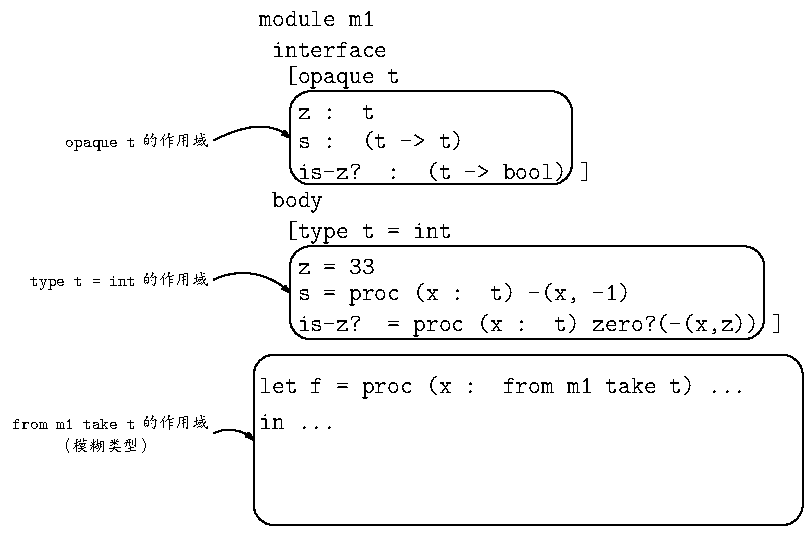
\includegraphics[scale=1.0]{module-type.pdf}\end{SCentered}

\caption{模块类型声明的作用域\label{t:x28elem_x22figx2d8x2e8x22x29}}\end{EoplFigure}

在接口的剩余部分中,声明 \Scribtexttt{transparent t = int} 将 \Scribtexttt{t} 绑定到类型 \Scribtexttt{int},
所以我们可以写 \Scribtexttt{z {\hbox{\texttt{:}}} t}。更重要的是,在程序的剩余部分中,声明也将 \Scribtexttt{from m1
take t} 绑定到 \Scribtexttt{int}。我们称之为\emph{受限类型} (\emph{qualified type})。
\index{szhou4xian4lei4xing2@受限类型|idxdecorator{}{}}
这里,我们用它声明了绑定到变量 \Scribtexttt{z} 的类型。声明的作用域是接口的剩余部分,以及
模块定义之后程序的剩余部分。

模块主体中的定义 \Scribtexttt{type t = int} 在主体的剩余部分中,将 \Scribtexttt{t} 绑定到 \Scribtexttt{int},
所以我们可以写 \Scribtexttt{s = proc (x {\hbox{\texttt{:}}} t) {\hbox{\texttt{.}}}{\hbox{\texttt{.}}}{\hbox{\texttt{.}}}}。像之前那样,定义的作用域是主体的剩余部
分(见)。

当然,我们可以给类型起任意名字,也可以声明多个类型。类型声明可以出现在接口中任意
位置,只要每个声明都先于使用。

\index{jzu4ti3lei4xing2@具体类型|)idxdecorator{}{}}
\index{tzou4ming2lei4xing2@透明类型|)idxdecorator{}{}}
\index{lzei4xing2suo1xie3@类型缩写|)idxdecorator{}{}}

\Ssubsubsubsectionstarx{模糊类型}{模糊类型}\label{t:x28part_x22s8x2e2x2dopaquex2dtypesx22x29}

\index{czhou1xiang4lei4xing2@抽象类型|(idxdecorator{}{}}
\index{mzo2hu2lei4xing2@模糊类型|(idxdecorator{}{}}
模块还可以用 \Scribtexttt{opaque{-}type} 声明输出\emph{模糊}类型。模糊类型有时又
称作\emph{抽象类型} (\emph{abstract type})。

\begin{EoplExample}\label{t:x28elem_x22egx2d8x2e7x22x29}我们把 程序中的透明类型替换为模糊
类型。得出的程序是

\begin{Subflow}\begin{EoplCodeInset}\begin{SVerbatim}\begin{SingleColumn}\Scribtexttt{module m1}

\Scribtexttt{}\mbox{\hphantom{\Scribtexttt{x}}}\Scribtexttt{interface}

\Scribtexttt{}\mbox{\hphantom{\Scribtexttt{xx}}}\Scribtexttt{[opaque t}

\Scribtexttt{}\mbox{\hphantom{\Scribtexttt{xxx}}}\Scribtexttt{z {\hbox{\texttt{:}}} t}

\Scribtexttt{}\mbox{\hphantom{\Scribtexttt{xxx}}}\Scribtexttt{s {\hbox{\texttt{:}}} (t {-}{\Stttextmore} t)}

\Scribtexttt{}\mbox{\hphantom{\Scribtexttt{xxx}}}\Scribtexttt{is{-}z{\hbox{\texttt{?}}} {\hbox{\texttt{:}}} (t {-}{\Stttextmore} bool)]}

\Scribtexttt{}\mbox{\hphantom{\Scribtexttt{x}}}\Scribtexttt{body}

\Scribtexttt{}\mbox{\hphantom{\Scribtexttt{xx}}}\Scribtexttt{[type t = int}

\Scribtexttt{}\mbox{\hphantom{\Scribtexttt{xxx}}}\Scribtexttt{z = 33}

\Scribtexttt{}\mbox{\hphantom{\Scribtexttt{xxx}}}\Scribtexttt{s = proc (x {\hbox{\texttt{:}}} t) {-}(x,{-}1)}

\Scribtexttt{}\mbox{\hphantom{\Scribtexttt{xxx}}}\Scribtexttt{is{-}z{\hbox{\texttt{?}}} = proc (x {\hbox{\texttt{:}}} t) zero{\hbox{\texttt{?}}}({-}(x,z))]}

\Scribtexttt{}\mbox{\hphantom{\Scribtexttt{x}}}

\Scribtexttt{}\mbox{\hphantom{\Scribtexttt{x}}}\Scribtexttt{proc (x {\hbox{\texttt{:}}} from m1 take t)}

\Scribtexttt{}\mbox{\hphantom{\Scribtexttt{xx}}}\Scribtexttt{(from m1 take is{-}z{\hbox{\texttt{?}}} {-}(x,0))}\end{SingleColumn}\end{SVerbatim}\end{EoplCodeInset}\end{Subflow}\end{EoplExample}

接口中的声明 \Scribtexttt{opaque t} 把 \Scribtexttt{t} 作为一种新的模糊类型名字。模糊类型的行为就
像 \Scribtexttt{int} 或 \Scribtexttt{bool} 之类的原生类型。名为 \Scribtexttt{t} 的类型在接口的剩余部分中绑
定到这种模糊类型,而受限类型 \Scribtexttt{from m1 take t} 在程序的剩余部分中绑定到同一模
糊类型。程序的剩余部分都知道 \Scribtexttt{from m1 take z} 绑定到一个值,其类型为 \Scribtexttt{from
m1 take t};\Scribtexttt{from m1 take s} 和 \Scribtexttt{from m1 take is{-}z{\hbox{\texttt{?}}}} 绑定到过程,用来处理
这种类型的值。\index{czhou1xiang4bian1jie4@抽象边界|idxdecorator{}{}}这就是抽象边界。类型检查器确保表
达式的类型为 \Scribtexttt{from m1 take t}时,求值是安全的,所以表达式的值只能通过这些操作
符生成,如suitable{-}env所述。

与之对应,定义 \Scribtexttt{type t = int} 在模块主体内部将 \Scribtexttt{t} 作为 \Scribtexttt{int} 的名字,
但是,由于程序的剩余部分从模块接口获得绑定,所以对此一无所知。

所以 \Scribtexttt{{-}(x,0)} 类型异常,因为主程序不知道类型 \Scribtexttt{from m1 take t} 为的值就是类
型为 \Scribtexttt{int} 的值。

我们改变程序,删掉算术操作,得

\begin{Subflow}\begin{EoplCodeInset}\begin{SVerbatim}\begin{SingleColumn}\Scribtexttt{module m1}

\Scribtexttt{}\mbox{\hphantom{\Scribtexttt{x}}}\Scribtexttt{interface}

\Scribtexttt{}\mbox{\hphantom{\Scribtexttt{xx}}}\Scribtexttt{[opaque t}

\Scribtexttt{}\mbox{\hphantom{\Scribtexttt{xxx}}}\Scribtexttt{z {\hbox{\texttt{:}}} t}

\Scribtexttt{}\mbox{\hphantom{\Scribtexttt{xxx}}}\Scribtexttt{s {\hbox{\texttt{:}}} (t {-}{\Stttextmore} t)}

\Scribtexttt{}\mbox{\hphantom{\Scribtexttt{xxx}}}\Scribtexttt{is{-}z{\hbox{\texttt{?}}} {\hbox{\texttt{:}}} (t {-}{\Stttextmore} bool)]}

\Scribtexttt{}\mbox{\hphantom{\Scribtexttt{x}}}\Scribtexttt{body}

\Scribtexttt{}\mbox{\hphantom{\Scribtexttt{xx}}}\Scribtexttt{[type t = int}

\Scribtexttt{}\mbox{\hphantom{\Scribtexttt{xxx}}}\Scribtexttt{z = 33}

\Scribtexttt{}\mbox{\hphantom{\Scribtexttt{xxx}}}\Scribtexttt{s = proc (x {\hbox{\texttt{:}}} t) {-}(x,{-}1)}

\Scribtexttt{}\mbox{\hphantom{\Scribtexttt{xxx}}}\Scribtexttt{is{-}z{\hbox{\texttt{?}}} = proc (x {\hbox{\texttt{:}}} t) zero{\hbox{\texttt{?}}}({-}(x,z))]}

\Scribtexttt{}\mbox{\hphantom{\Scribtexttt{x}}}

\Scribtexttt{}\mbox{\hphantom{\Scribtexttt{x}}}\Scribtexttt{proc (x {\hbox{\texttt{:}}} from m1 take t)}

\Scribtexttt{}\mbox{\hphantom{\Scribtexttt{xx}}}\Scribtexttt{(from m1 take is{-}z{\hbox{\texttt{?}}} x)}\end{SingleColumn}\end{SVerbatim}\end{EoplCodeInset}

现在,我们的程序类型正常,类型为 \Scribtexttt{(from m1 take t {-}{\Stttextmore} bool)}。\end{Subflow}

通过强化抽象边界,类型检查器确保程序只能通过接口提供的过程处理接口提供的值。
如\ChapRefLocal{t:x28part_x22dax22x29}{2}{数据抽象}所述,这给我们提供了机制来分离数据类型的用户和实现。接下来,我们给
出这一技术的几个例子。

\begin{EoplExample}\label{t:x28elem_x22egx2d8x2e8x22x29}如果程序使用了模块定义

\begin{Subflow}\begin{EoplCodeInset}\begin{SVerbatim}\begin{SingleColumn}\Scribtexttt{module colors}

\Scribtexttt{}\mbox{\hphantom{\Scribtexttt{x}}}\Scribtexttt{interface}

\Scribtexttt{}\mbox{\hphantom{\Scribtexttt{xx}}}\Scribtexttt{[opaque color}

\Scribtexttt{}\mbox{\hphantom{\Scribtexttt{xxx}}}\Scribtexttt{red {\hbox{\texttt{:}}} color}

\Scribtexttt{}\mbox{\hphantom{\Scribtexttt{xxx}}}\Scribtexttt{green {\hbox{\texttt{:}}} color}

\Scribtexttt{}\mbox{\hphantom{\Scribtexttt{xxx}}}\Scribtexttt{is{-}red{\hbox{\texttt{?}}} {\hbox{\texttt{:}}} (color {-}{\Stttextmore} bool)]}

\Scribtexttt{}\mbox{\hphantom{\Scribtexttt{x}}}\Scribtexttt{body}

\Scribtexttt{}\mbox{\hphantom{\Scribtexttt{xx}}}\Scribtexttt{[type color = int}

\Scribtexttt{}\mbox{\hphantom{\Scribtexttt{xxx}}}\Scribtexttt{red = 0}

\Scribtexttt{}\mbox{\hphantom{\Scribtexttt{xxx}}}\Scribtexttt{green = 1}

\Scribtexttt{}\mbox{\hphantom{\Scribtexttt{xxx}}}\Scribtexttt{is{-}red{\hbox{\texttt{?}}} = proc (c {\hbox{\texttt{:}}} color) zero{\hbox{\texttt{?}}}(c)]}\end{SingleColumn}\end{SVerbatim}\end{EoplCodeInset}

程序没法知道 \Scribtexttt{from colors take color} 实际为 \Scribtexttt{int},也不知道 \Scribtexttt{from
colors take green} 实际为 1(也许有一个例外:返回颜色作为最终答案,然后打印出
来)。\end{Subflow}\end{EoplExample}

\begin{EoplExample}\label{t:x28elem_x22egx2d8x2e9x22x29}程序

\begin{Subflow}\begin{EoplCodeInset}\begin{SVerbatim}\begin{SingleColumn}\Scribtexttt{module ints1}

\Scribtexttt{}\mbox{\hphantom{\Scribtexttt{x}}}\Scribtexttt{interface}

\Scribtexttt{}\mbox{\hphantom{\Scribtexttt{xx}}}\Scribtexttt{[opaque t}

\Scribtexttt{}\mbox{\hphantom{\Scribtexttt{xxx}}}\Scribtexttt{zero {\hbox{\texttt{:}}} t}

\Scribtexttt{}\mbox{\hphantom{\Scribtexttt{xxx}}}\Scribtexttt{succ {\hbox{\texttt{:}}} (t {-}{\Stttextmore} t)}

\Scribtexttt{}\mbox{\hphantom{\Scribtexttt{xxx}}}\Scribtexttt{pred {\hbox{\texttt{:}}} (t {-}{\Stttextmore} t)}

\Scribtexttt{}\mbox{\hphantom{\Scribtexttt{xxx}}}\Scribtexttt{is{-}zero {\hbox{\texttt{:}}} (t {-}{\Stttextmore} bool)]}

\Scribtexttt{}\mbox{\hphantom{\Scribtexttt{x}}}\Scribtexttt{body}

\Scribtexttt{}\mbox{\hphantom{\Scribtexttt{xx}}}\Scribtexttt{[type t = int}

\Scribtexttt{}\mbox{\hphantom{\Scribtexttt{xxx}}}\Scribtexttt{zero = 0}

\Scribtexttt{}\mbox{\hphantom{\Scribtexttt{xxx}}}\Scribtexttt{succ = proc(x {\hbox{\texttt{:}}} t) {-}(x,{-}5)}

\Scribtexttt{}\mbox{\hphantom{\Scribtexttt{xxx}}}\Scribtexttt{pred = proc(x {\hbox{\texttt{:}}} t) {-}(x,5)}

\Scribtexttt{}\mbox{\hphantom{\Scribtexttt{xxx}}}\Scribtexttt{is{-}zero = proc (x {\hbox{\texttt{:}}} t) zero{\hbox{\texttt{?}}}(x)]}

\Scribtexttt{}\mbox{\hphantom{\Scribtexttt{x}}}

\Scribtexttt{let z = from ints1 take zero}

\Scribtexttt{in let s = from ints1 take succ}

\Scribtexttt{}\mbox{\hphantom{\Scribtexttt{xxx}}}\Scribtexttt{in (s (s z))}\end{SingleColumn}\end{SVerbatim}\end{EoplCodeInset}

类型为 \Scribtexttt{from ints1 take t},值为 10。但我们只能通过 \Scribtexttt{ints1} 输出的过程处理
这个值。这个模块用表达值 \texMathInline{5*k} 表示整数 \texMathInline{k}。用\SecRefLocal{t:x28part_x22s2x2e1x22x29}{2.1}{用接口定义数据}的表示法,写作
\texMathInline{\lceil k \rceil = 5 * k}。\end{Subflow}\end{EoplExample}

\begin{EoplExample}\label{t:x28elem_x22egx2d8x2e10x22x29}在这个模块中,\texMathInline{\lceil k \rceil = -3 * k}。

\begin{Subflow}\begin{EoplCodeInset}\begin{SVerbatim}\begin{SingleColumn}\Scribtexttt{module ints2}

\Scribtexttt{}\mbox{\hphantom{\Scribtexttt{x}}}\Scribtexttt{interface}

\Scribtexttt{}\mbox{\hphantom{\Scribtexttt{xx}}}\Scribtexttt{[opaque t}

\Scribtexttt{}\mbox{\hphantom{\Scribtexttt{xxx}}}\Scribtexttt{zero {\hbox{\texttt{:}}} t}

\Scribtexttt{}\mbox{\hphantom{\Scribtexttt{xxx}}}\Scribtexttt{succ {\hbox{\texttt{:}}} (t {-}{\Stttextmore} t)}

\Scribtexttt{}\mbox{\hphantom{\Scribtexttt{xxx}}}\Scribtexttt{pred {\hbox{\texttt{:}}} (t {-}{\Stttextmore} t)}

\Scribtexttt{}\mbox{\hphantom{\Scribtexttt{xxx}}}\Scribtexttt{is{-}zero {\hbox{\texttt{:}}} (t {-}{\Stttextmore} bool)]}

\Scribtexttt{}\mbox{\hphantom{\Scribtexttt{x}}}\Scribtexttt{body}

\Scribtexttt{}\mbox{\hphantom{\Scribtexttt{xx}}}\Scribtexttt{[type t = int}

\Scribtexttt{}\mbox{\hphantom{\Scribtexttt{xxx}}}\Scribtexttt{zero = 0}

\Scribtexttt{}\mbox{\hphantom{\Scribtexttt{xxx}}}\Scribtexttt{succ = proc(x {\hbox{\texttt{:}}} t) {-}(x,3)}

\Scribtexttt{}\mbox{\hphantom{\Scribtexttt{xxx}}}\Scribtexttt{pred = proc(x {\hbox{\texttt{:}}} t) {-}(x,{-}3)}

\Scribtexttt{}\mbox{\hphantom{\Scribtexttt{xxx}}}\Scribtexttt{is{-}zero = proc (x {\hbox{\texttt{:}}} t) zero{\hbox{\texttt{?}}}(x)]}

\Scribtexttt{}\mbox{\hphantom{\Scribtexttt{x}}}

\Scribtexttt{let z = from ints2 take zero}

\Scribtexttt{in let s = from ints2 take succ}

\Scribtexttt{}\mbox{\hphantom{\Scribtexttt{xxx}}}\Scribtexttt{in (s (s z))}\end{SingleColumn}\end{SVerbatim}\end{EoplCodeInset}

类型为 \Scribtexttt{from ints2 take t},值为 {-}6。\end{Subflow}\end{EoplExample}

\begin{EoplExample}\label{t:x28elem_x22egx2d8x2e11x22x29}在前面的例子中,我们不能直接处理值,但我们能用模块输出
的过程处理它们。像\ChapRefLocal{t:x28part_x22dax22x29}{2}{数据抽象}那样,我们可以结合这些过程做有用的工作。这里,我们
将它们结合起来,写出过程 \Scribtexttt{to{-}int},把模块中的值转回 \Scribtexttt{int} 类型。

\begin{Subflow}\begin{EoplCodeInset}\begin{SVerbatim}\begin{SingleColumn}\Scribtexttt{module ints1 }\emph{...同前...}\Scribtexttt{}

\Scribtexttt{}\mbox{\hphantom{\Scribtexttt{x}}}

\Scribtexttt{let z = from ints1 take zero}

\Scribtexttt{in let s = from ints1 take succ}

\Scribtexttt{in let p = from ints1 take pred}

\Scribtexttt{in let z{\hbox{\texttt{?}}} = from ints1 take is{-}zero}

\Scribtexttt{in letrec int to{-}int (x {\hbox{\texttt{:}}} from ints1 take t) =}

\Scribtexttt{}\mbox{\hphantom{\Scribtexttt{xxxxxxxxxxxxxx}}}\Scribtexttt{if (z{\hbox{\texttt{?}}} x)}

\Scribtexttt{}\mbox{\hphantom{\Scribtexttt{xxxxxxxxxxxxxx}}}\Scribtexttt{then 0}

\Scribtexttt{}\mbox{\hphantom{\Scribtexttt{xxxxxxxxxxxxxx}}}\Scribtexttt{else {-}((to{-}int (p x)), {-}1)}

\Scribtexttt{in (to{-}int (s (s z)))}\end{SingleColumn}\end{SVerbatim}\end{EoplCodeInset}

类型为 \Scribtexttt{int},值为 2。\end{Subflow}\end{EoplExample}

\begin{EoplExample}\label{t:x28elem_x22egx2d8x2e12x22x29}这里用到的技术与 \Scribtexttt{ints2} 中算术操作的实现相同。

\begin{Subflow}\begin{EoplCodeInset}\begin{SVerbatim}\begin{SingleColumn}\Scribtexttt{module ints2 }\emph{...同前...}\Scribtexttt{}

\Scribtexttt{}\mbox{\hphantom{\Scribtexttt{x}}}

\Scribtexttt{let z = from ints2 take zero}

\Scribtexttt{in let s = from ints2 take succ}

\Scribtexttt{in let p = from ints2 take pred}

\Scribtexttt{in let z{\hbox{\texttt{?}}} = from ints2 take is{-}zero}

\Scribtexttt{in letrec int to{-}int (x {\hbox{\texttt{:}}} from ints2 take t) =}

\Scribtexttt{}\mbox{\hphantom{\Scribtexttt{xxxxxxxxxxxxxx}}}\Scribtexttt{if (z{\hbox{\texttt{?}}} x)}

\Scribtexttt{}\mbox{\hphantom{\Scribtexttt{xxxxxxxxxxxxxx}}}\Scribtexttt{then 0}

\Scribtexttt{}\mbox{\hphantom{\Scribtexttt{xxxxxxxxxxxxxx}}}\Scribtexttt{else {-}((to{-}int (p x)), {-}1)}

\Scribtexttt{in (to{-}int (s (s z)))}\end{SingleColumn}\end{SVerbatim}\end{EoplCodeInset}

类型同样为 \Scribtexttt{int},值为 2。\end{Subflow}\end{EoplExample}

在\SecRefLocal{t:x28part_x22s8x2e3x22x29}{8.3}{模块过程}中,我们展示如何将两个抽象出来。

\begin{EoplExample}\label{t:x28elem_x22egx2d8x2e13x22x29}在下面的程序中,我们设计一个模块来封装布尔类型。布尔值用整数值表示,
但是像 那样,程序的剩余部分对此一无所知。

\begin{Subflow}\begin{EoplCodeInset}\begin{SVerbatim}\begin{SingleColumn}\Scribtexttt{module mybool}

\Scribtexttt{}\mbox{\hphantom{\Scribtexttt{x}}}\Scribtexttt{interface}

\Scribtexttt{}\mbox{\hphantom{\Scribtexttt{xx}}}\Scribtexttt{[opaque t}

\Scribtexttt{}\mbox{\hphantom{\Scribtexttt{xxx}}}\Scribtexttt{true {\hbox{\texttt{:}}} t}

\Scribtexttt{}\mbox{\hphantom{\Scribtexttt{xxx}}}\Scribtexttt{false {\hbox{\texttt{:}}} t}

\Scribtexttt{}\mbox{\hphantom{\Scribtexttt{xxx}}}\Scribtexttt{and {\hbox{\texttt{:}}} (t {-}{\Stttextmore} (t {-}{\Stttextmore} t))}

\Scribtexttt{}\mbox{\hphantom{\Scribtexttt{xxx}}}\Scribtexttt{not {\hbox{\texttt{:}}} (t {-}{\Stttextmore} t)}

\Scribtexttt{}\mbox{\hphantom{\Scribtexttt{xxx}}}\Scribtexttt{to{-}bool {\hbox{\texttt{:}}} (t {-}{\Stttextmore} bool)]}

\Scribtexttt{}\mbox{\hphantom{\Scribtexttt{x}}}\Scribtexttt{body}

\Scribtexttt{}\mbox{\hphantom{\Scribtexttt{xx}}}\Scribtexttt{[type t = int}

\Scribtexttt{}\mbox{\hphantom{\Scribtexttt{xxx}}}\Scribtexttt{true = 0}

\Scribtexttt{}\mbox{\hphantom{\Scribtexttt{xxx}}}\Scribtexttt{false = 13}

\Scribtexttt{}\mbox{\hphantom{\Scribtexttt{xxx}}}\Scribtexttt{and = proc (x {\hbox{\texttt{:}}} t)}

\Scribtexttt{}\mbox{\hphantom{\Scribtexttt{xxxxxxxxxx}}}\Scribtexttt{proc (y {\hbox{\texttt{:}}} t)}

\Scribtexttt{}\mbox{\hphantom{\Scribtexttt{xxxxxxxxxxx}}}\Scribtexttt{if zero{\hbox{\texttt{?}}}(x) then y else false}

\Scribtexttt{}\mbox{\hphantom{\Scribtexttt{xxx}}}\Scribtexttt{not = proc (x {\hbox{\texttt{:}}} t)}

\Scribtexttt{}\mbox{\hphantom{\Scribtexttt{xxxxxxxxxxx}}}\Scribtexttt{if zero{\hbox{\texttt{?}}}(x) then false else true}

\Scribtexttt{}\mbox{\hphantom{\Scribtexttt{xxx}}}\Scribtexttt{to{-}bool = proc (x {\hbox{\texttt{:}}} t) zero{\hbox{\texttt{?}}}(x)]}

\Scribtexttt{}\mbox{\hphantom{\Scribtexttt{x}}}

\Scribtexttt{let true = from mybool take true}

\Scribtexttt{in let false = from mybool take false}

\Scribtexttt{}\mbox{\hphantom{\Scribtexttt{xxx}}}\Scribtexttt{in let and = from mybool take and}

\Scribtexttt{}\mbox{\hphantom{\Scribtexttt{xxxxxx}}}\Scribtexttt{in ((and true) false)}\end{SingleColumn}\end{SVerbatim}\end{EoplCodeInset}

类型为 \Scribtexttt{from mybool take t},值为 13。\end{Subflow}\end{EoplExample}

\index{czhou1xiang4lei4xing2@抽象类型|)idxdecorator{}{}}
\index{mzo2hu2lei4xing2@模糊类型|)idxdecorator{}{}}

\begin{EoplExercise}\label{t:x28elem_x22ex8x2e12x22x29}\texMathInline{\textnormal{[}{\star}\textnormal{]}}\mbox{\hphantom{\Scribtexttt{x}}}在 中,\Scribtexttt{and} 和 \Scribtexttt{not} 的定义可以从模块内部移到外面
吗?\Scribtexttt{to{-}bool} 呢?\end{EoplExercise}

\begin{EoplExercise}\label{t:x28elem_x22ex8x2e13x22x29}\texMathInline{\textnormal{[}{\star}\textnormal{]}}\mbox{\hphantom{\Scribtexttt{x}}}写一个模块,用 \texMathInline{5*k+3} 表示整数 \texMathInline{k},实现算术操作。\end{EoplExercise}

\begin{EoplExercise}\label{t:x28elem_x22ex8x2e14x22x29}\texMathInline{\textnormal{[}{\star}\textnormal{]}}\mbox{\hphantom{\Scribtexttt{x}}}下面是 \Scribtexttt{mybool}()的另一种定义:

\begin{EoplCodeInset}\begin{SVerbatim}\begin{SingleColumn}\Scribtexttt{module mybool}

\Scribtexttt{}\mbox{\hphantom{\Scribtexttt{x}}}\Scribtexttt{interface}

\Scribtexttt{}\mbox{\hphantom{\Scribtexttt{xx}}}\Scribtexttt{[opaque t}

\Scribtexttt{}\mbox{\hphantom{\Scribtexttt{xxx}}}\Scribtexttt{true {\hbox{\texttt{:}}} t}

\Scribtexttt{}\mbox{\hphantom{\Scribtexttt{xxx}}}\Scribtexttt{false {\hbox{\texttt{:}}} t}

\Scribtexttt{}\mbox{\hphantom{\Scribtexttt{xxx}}}\Scribtexttt{and {\hbox{\texttt{:}}} (t {-}{\Stttextmore} (t {-}{\Stttextmore} t))}

\Scribtexttt{}\mbox{\hphantom{\Scribtexttt{xxx}}}\Scribtexttt{not {\hbox{\texttt{:}}} (t {-}{\Stttextmore} t)}

\Scribtexttt{}\mbox{\hphantom{\Scribtexttt{xxx}}}\Scribtexttt{to{-}bool {\hbox{\texttt{:}}} (t {-}{\Stttextmore} bool)]}

\Scribtexttt{}\mbox{\hphantom{\Scribtexttt{x}}}\Scribtexttt{body}

\Scribtexttt{}\mbox{\hphantom{\Scribtexttt{xx}}}\Scribtexttt{[type t = int}

\Scribtexttt{}\mbox{\hphantom{\Scribtexttt{xxx}}}\Scribtexttt{true = 1}

\Scribtexttt{}\mbox{\hphantom{\Scribtexttt{xxx}}}\Scribtexttt{false = 0}

\Scribtexttt{}\mbox{\hphantom{\Scribtexttt{xxx}}}\Scribtexttt{and = proc (x {\hbox{\texttt{:}}} t)}

\Scribtexttt{}\mbox{\hphantom{\Scribtexttt{xxxxxxxxxx}}}\Scribtexttt{proc (y {\hbox{\texttt{:}}} t)}

\Scribtexttt{}\mbox{\hphantom{\Scribtexttt{xxxxxxxxxxx}}}\Scribtexttt{if zero{\hbox{\texttt{?}}}(x) then false else y}

\Scribtexttt{}\mbox{\hphantom{\Scribtexttt{xxx}}}\Scribtexttt{not = proc (x {\hbox{\texttt{:}}} t)}

\Scribtexttt{}\mbox{\hphantom{\Scribtexttt{xxxxxxxxxx}}}\Scribtexttt{if zero{\hbox{\texttt{?}}}(x) then true else false}

\Scribtexttt{}\mbox{\hphantom{\Scribtexttt{xxx}}}\Scribtexttt{to{-}bool = proc (x {\hbox{\texttt{:}}} t)}

\Scribtexttt{}\mbox{\hphantom{\Scribtexttt{xxxxxxxxxxxxxx}}}\Scribtexttt{if zero{\hbox{\texttt{?}}}(x) then zero{\hbox{\texttt{?}}}(1) else zero{\hbox{\texttt{?}}}(0)]}\end{SingleColumn}\end{SVerbatim}\end{EoplCodeInset}

有没有程序类型为 \Scribtexttt{int},用 \Scribtexttt{mybool} 原来的定义返回一个值,用新的定义返回另
一个值?\end{EoplExercise}

\begin{EoplExercise}\label{t:x28elem_x22ex8x2e15x22x29}\texMathInline{\textnormal{[}{\star}{\star}\textnormal{]}}\mbox{\hphantom{\Scribtexttt{x}}}\index{kze1li3hua4@柯里化|(idxdecorator{}{}}
\index{bziao3@表|(idxdecorator{}{}}
写一个模块,实现抽象表。你实现的表应类似环境,但不是把符号绑定到 Scheme 值,而是
把整数值绑定到整数值。接口提供一个值,表示空表;两个过程 \Scribtexttt{add{-}to{-}table} 和
\Scribtexttt{lookup{-}in{-}table} 类似 \Scribtexttt{extend{-}env} 和 \Scribtexttt{apply{-}env}。由于我们的语言只有
单参数过程,我们用咖喱化(ex3.20)实现等效的多参数过程。你可以用
查询任何值都返回 0 的表模拟空表。这是该模块的一个例子:

\begin{EoplCodeInset}\begin{SVerbatim}\begin{SingleColumn}\Scribtexttt{module tables}

\Scribtexttt{}\mbox{\hphantom{\Scribtexttt{x}}}\Scribtexttt{interface}

\Scribtexttt{}\mbox{\hphantom{\Scribtexttt{xx}}}\Scribtexttt{[opaque table}

\Scribtexttt{}\mbox{\hphantom{\Scribtexttt{xxx}}}\Scribtexttt{empty {\hbox{\texttt{:}}} table}

\Scribtexttt{}\mbox{\hphantom{\Scribtexttt{xxx}}}\Scribtexttt{add{-}to{-}table {\hbox{\texttt{:}}} (int {-}{\Stttextmore} (int {-}{\Stttextmore} (table {-}{\Stttextmore} table)))}

\Scribtexttt{}\mbox{\hphantom{\Scribtexttt{xxx}}}\Scribtexttt{lookup{-}in{-}table {\hbox{\texttt{:}}} (int {-}{\Stttextmore} (table {-}{\Stttextmore} int))]}

\Scribtexttt{}\mbox{\hphantom{\Scribtexttt{x}}}\Scribtexttt{body}

\Scribtexttt{}\mbox{\hphantom{\Scribtexttt{xx}}}\Scribtexttt{[type table = (int {-}{\Stttextmore} int)}

\Scribtexttt{}\mbox{\hphantom{\Scribtexttt{xxx}}}\Scribtexttt{{\hbox{\texttt{.}}}{\hbox{\texttt{.}}}{\hbox{\texttt{.}}}]}

\Scribtexttt{}\mbox{\hphantom{\Scribtexttt{x}}}

\Scribtexttt{let empty = from tables take empty}

\Scribtexttt{in let add{-}binding = from tables take add{-}to{-}table}

\Scribtexttt{}\mbox{\hphantom{\Scribtexttt{xxx}}}\Scribtexttt{in let lookup = from tables take lookup{-}in{-}table}

\Scribtexttt{}\mbox{\hphantom{\Scribtexttt{xxxxxx}}}\Scribtexttt{in let table1 = (((add{-}binding 3) 300)}

\Scribtexttt{}\mbox{\hphantom{\Scribtexttt{xxxxxxxxxxxxxxxxxxxxxxx}}}\Scribtexttt{(((add{-}binding 4) 400)}

\Scribtexttt{}\mbox{\hphantom{\Scribtexttt{xxxxxxxxxxxxxxxxxxxxxxxx}}}\Scribtexttt{(((add{-}binding 3) 600)}

\Scribtexttt{}\mbox{\hphantom{\Scribtexttt{xxxxxxxxxxxxxxxxxxxxxxxxx}}}\Scribtexttt{empty)))}

\Scribtexttt{}\mbox{\hphantom{\Scribtexttt{xxxxxxxxx}}}\Scribtexttt{in {-}(((lookup 4) table1),}

\Scribtexttt{}\mbox{\hphantom{\Scribtexttt{xxxxxxxxxxxxxx}}}\Scribtexttt{((lookup 3) table1))}\end{SingleColumn}\end{SVerbatim}\end{EoplCodeInset}

这个程序类型应为 \Scribtexttt{int}。表 \Scribtexttt{table1} 把 4 绑定到 400,把 3 绑定到 300,所以
程序的值应为 100。
\index{kze1li3hua4@柯里化|)idxdecorator{}{}}
\index{bziao3@表|)idxdecorator{}{}}\end{EoplExercise}

\Ssubsubsection{实现}{实现}\label{t:x28part_x22s8x2e2x2e2x22x29}

现在我们来扩展系统,实现透明类型和模糊类型声明,及受限类型的引用。

\Ssubsubsubsectionstarx{语法和解释器}{语法和解释器}\label{t:x28part_x22syntaxx2dandx2dthex2dinterpreterx22x29}

\index{szhou4xian4lei4xing2@受限类型|idxdecorator{}{}}
\index{valueof@\textbf{\Scribtexttt{value{-}of}}!OPAQUETYPES@OPAQUE{-}TYPES|(idxdecorator{}{}}
我们给两种新类型添加语法:有名类型(如 \Scribtexttt{t})和受限类型(如 \Scribtexttt{from m1 take
t})。

\begin{Small}\Iidentity{\begin{align*}\mathit{Type} &::= \mathit{Identifier} \\[-3pt]
&\mathrel{\phantom{::=}} \fbox{\Scribtexttt{named{-}type (name)}} \\[5pt]
    \mathit{Type} &::= \Scribtexttt{from }\Iidentity{\mathit{Identifier}}\Scribtexttt{ take }\Iidentity{\mathit{Identifier}} \\[-3pt]
&\mathrel{\phantom{::=}} \fbox{\Scribtexttt{qualified{-}type (m{-}name t{-}name)}}\end{align*}}\end{Small}

我们为模糊类型和透明类型新增两种声明。

\begin{Small}\Iidentity{\begin{align*}\mathit{Decl} &::= \Scribtexttt{opaque }\Iidentity{\mathit{Identifier}} \\[-3pt]
&\mathrel{\phantom{::=}} \fbox{\Scribtexttt{opaque{-}type{-}decl (t{-}name)}} \\[5pt]
    \mathit{Decl} &::= \Scribtexttt{transparent }\Iidentity{\mathit{Identifier}}\Scribtexttt{ = }\Iidentity{\mathit{Type}} \\[-3pt]
&\mathrel{\phantom{::=}} \fbox{\Scribtexttt{transparent{-}type{-}decl (t{-}name ty)}}\end{align*}}\end{Small}

\index{lzei4xing2ding4yi4@类型定义|idxdecorator{}{}}
我们还要新增一种定义:类型定义,用来定义模糊类型和透明类型。

\begin{Small}\Iidentity{\begin{align*}\mathit{Defn} &::= \Scribtexttt{type }\Iidentity{\mathit{Identifier}}\Scribtexttt{ = }\Iidentity{\mathit{Type}} \\[-3pt]
&\mathrel{\phantom{::=}} \fbox{\Scribtexttt{type{-}defn (name ty)}}\end{align*}}\end{Small}

解释器不需要查看类型和声明,所以解释器的唯一改动是忽略类型定义。

\begin{EoplCodeInset}\begin{SCodeFlow}\begin{RktBlk}\begin{SingleColumn}\textbf{\Scribtexttt{defns{-}to{-}env}} : \texMathInline{\mathit{Listof(Defn)} \times \mathit{Env} \to \mathit{Env}}

\RktPn{(}\RktSym{define}\mbox{\hphantom{\Scribtexttt{x}}}\RktSym{defns{-}to{-}env}

\mbox{\hphantom{\Scribtexttt{xx}}}\RktPn{(}\RktSym{lambda}\mbox{\hphantom{\Scribtexttt{x}}}\RktPn{(}\RktSym{defns}\mbox{\hphantom{\Scribtexttt{x}}}\RktSym{env}\RktPn{)}

\mbox{\hphantom{\Scribtexttt{xxxx}}}\RktPn{(}\RktSym{if}\mbox{\hphantom{\Scribtexttt{x}}}\RktPn{(}\RktSym{null{\hbox{\texttt{?}}}}\mbox{\hphantom{\Scribtexttt{x}}}\RktSym{defns}\RktPn{)}

\mbox{\hphantom{\Scribtexttt{xxxxxx}}}\RktPn{(}\RktSym{empty{-}env}\RktPn{)}

\mbox{\hphantom{\Scribtexttt{xxxxxx}}}\RktPn{(}\RktSym{cases}\mbox{\hphantom{\Scribtexttt{x}}}\RktSym{definition}\mbox{\hphantom{\Scribtexttt{x}}}\RktPn{(}\RktSym{car}\mbox{\hphantom{\Scribtexttt{x}}}\RktSym{defns}\RktPn{)}

\mbox{\hphantom{\Scribtexttt{xxxxxxxx}}}\RktPn{(}\RktSym{val{-}defn}\mbox{\hphantom{\Scribtexttt{x}}}\RktPn{(}\RktSym{var}\mbox{\hphantom{\Scribtexttt{x}}}\RktSym{exp}\RktPn{)}\mbox{\hphantom{\Scribtexttt{x}}}\RktSym{{\hbox{\texttt{.}}}{\hbox{\texttt{.}}}{\hbox{\texttt{.}}}as}\mbox{\hphantom{\Scribtexttt{x}}}\RktSym{before{\hbox{\texttt{.}}}{\hbox{\texttt{.}}}{\hbox{\texttt{.}}}}\RktPn{)}

\mbox{\hphantom{\Scribtexttt{xxxxxxxx}}}\RktPn{(}\RktSym{type{-}defn}\mbox{\hphantom{\Scribtexttt{x}}}\RktPn{(}\RktSym{type{-}name}\mbox{\hphantom{\Scribtexttt{x}}}\RktSym{type}\RktPn{)}

\mbox{\hphantom{\Scribtexttt{xxxxxxxxxx}}}\RktPn{(}\RktSym{defns{-}to{-}env}\mbox{\hphantom{\Scribtexttt{x}}}\RktPn{(}\RktSym{cdr}\mbox{\hphantom{\Scribtexttt{x}}}\RktSym{defns}\RktPn{)}\mbox{\hphantom{\Scribtexttt{x}}}\RktSym{env}\RktPn{)}\RktPn{)}\RktPn{)}\RktPn{)}\RktPn{)}\RktPn{)}\end{SingleColumn}\end{RktBlk}\end{SCodeFlow}

\noindent \index{valueof@\textbf{\Scribtexttt{value{-}of}}!OPAQUETYPES@OPAQUE{-}TYPES|)idxdecorator{}{}}\end{EoplCodeInset}

\Ssubsubsubsectionstarx{检查器}{检查器}\label{t:x28part_x22thex2dcheckerx22x29}

\index{lzei4xing2jian3cha2@类型检查!mzo2kuai4@模块|(idxdecorator{}{}}
\index{lzei4xing2jie2gou4@类型结构!mzo2hu2he2tou4ming2lei4xing2@模糊和透明类型|(idxdecorator{}{}}
检查器的改动就多多了,因为所有关于类型的操作都要扩展,以便处理新的类型。

首先,我们介绍一种系统性的方法来处理模糊类型和透明类型。模糊类型就像 \Scribtexttt{int} 或
\Scribtexttt{bool} 之类的原生类型一样。而透明类型名副其实,是透明的:它们的行为与定义相同。
所以每个类型都等价于下列语法描述的:

\begin{Subflow}\begin{Small}\texMathDisplay{\mathit{Type} ::= \Scribtexttt{int}\ |\ \Scribtexttt{bool}\ |\ \Scribtexttt{from }\texMathInline{m}\Scribtexttt{ take }\texMathInline{t}\ |\ \Scribtexttt{(}\texMathInline{\mathit{Type}}\Scribtexttt{ {-}{\Stttextmore} }\texMathInline{\mathit{Type}}\Scribtexttt{)}}\end{Small}

其中,\texMathInline{t} 为 \texMathInline{m} 中的模糊类型声明。我们称这种形式的类型为\emph{展开类型} (\emph{expanded
type})。\end{Subflow}

接下来我们扩展类型环境,处理新类型。我们的类型环境将每个有名类型或受限类型绑定到
一个展开类型。新的类型环境定义为

\begin{Subflow}\begin{EoplCodeInset}\begin{SCodeFlow}\begin{RktBlk}\begin{SingleColumn}\RktPn{(}\RktSym{define{-}datatype}\mbox{\hphantom{\Scribtexttt{x}}}\RktSym{type{-}environment}\mbox{\hphantom{\Scribtexttt{x}}}\RktSym{type{-}environment{\hbox{\texttt{?}}}}

\mbox{\hphantom{\Scribtexttt{xx}}}\RktPn{(}\RktSym{empty{-}tenv}\RktPn{)}

\mbox{\hphantom{\Scribtexttt{xx}}}\RktPn{(}\RktSym{extend{-}tenv}\mbox{\hphantom{\Scribtexttt{x}}}\emph{...同前...}\RktPn{)}

\mbox{\hphantom{\Scribtexttt{xx}}}\RktPn{(}\RktSym{extend{-}tenv{-}with{-}module}\mbox{\hphantom{\Scribtexttt{x}}}\emph{...同前...}\RktPn{)}

\mbox{\hphantom{\Scribtexttt{xx}}}\RktPn{(}\RktSym{extend{-}tenv{-}with{-}type}

\mbox{\hphantom{\Scribtexttt{xxxx}}}\RktPn{(}\RktSym{t{-}name}\mbox{\hphantom{\Scribtexttt{x}}}\RktSym{symbol{\hbox{\texttt{?}}}}\RktPn{)}

\mbox{\hphantom{\Scribtexttt{xxxx}}}\RktPn{(}\RktSym{type}\mbox{\hphantom{\Scribtexttt{x}}}\RktSym{type{\hbox{\texttt{?}}}}\RktPn{)}

\mbox{\hphantom{\Scribtexttt{xxxx}}}\RktPn{(}\RktSym{saved{-}tenv}\mbox{\hphantom{\Scribtexttt{x}}}\RktSym{type{-}environment{\hbox{\texttt{?}}}}\RktPn{)}\RktPn{)}\RktPn{)}\end{SingleColumn}\end{RktBlk}\end{SCodeFlow}\end{EoplCodeInset}

它满足条件:\Scribtexttt{type} 总是一个展开类型。像invariant讨论的,这个条件是
一\emph{不变式}。\end{Subflow}

\index{zzhan3kai1lei4xing2@展开类型|(idxdecorator{}{}}
接着我们写出函数 \Scribtexttt{expand{-}type},它取一个类型和一个类型环境,用后者中的绑定展
开前者。根据不变式“结果类型已展开”,它在类型环境中查
询有名类型和受限类型,对\Scribtexttt{proc} 类型,它递归处理参数和结果类型。

\begin{EoplCodeInset}\begin{SCodeFlow}\begin{RktBlk}\begin{SingleColumn}\textbf{\Scribtexttt{expand{-}type}} : \texMathInline{\mathit{Type} \times \mathit{Tenv} \to \mathit{ExpandedType}}

\RktPn{(}\RktSym{define}\mbox{\hphantom{\Scribtexttt{x}}}\RktSym{expand{-}type}

\mbox{\hphantom{\Scribtexttt{xx}}}\RktPn{(}\RktSym{lambda}\mbox{\hphantom{\Scribtexttt{x}}}\RktPn{(}\RktSym{ty}\mbox{\hphantom{\Scribtexttt{x}}}\RktSym{tenv}\RktPn{)}

\mbox{\hphantom{\Scribtexttt{xxxx}}}\RktPn{(}\RktSym{cases}\mbox{\hphantom{\Scribtexttt{x}}}\RktSym{type}\mbox{\hphantom{\Scribtexttt{x}}}\RktSym{ty}

\mbox{\hphantom{\Scribtexttt{xxxxxx}}}\RktPn{(}\RktSym{int{-}type}\mbox{\hphantom{\Scribtexttt{x}}}\RktPn{(}\RktPn{)}\mbox{\hphantom{\Scribtexttt{x}}}\RktPn{(}\RktSym{int{-}type}\RktPn{)}\RktPn{)}

\mbox{\hphantom{\Scribtexttt{xxxxxx}}}\RktPn{(}\RktSym{bool{-}type}\mbox{\hphantom{\Scribtexttt{x}}}\RktPn{(}\RktPn{)}\mbox{\hphantom{\Scribtexttt{x}}}\RktPn{(}\RktSym{bool{-}type}\RktPn{)}\RktPn{)}

\mbox{\hphantom{\Scribtexttt{xxxxxx}}}\RktPn{(}\RktSym{proc{-}type}\mbox{\hphantom{\Scribtexttt{x}}}\RktPn{(}\RktSym{arg{-}type}\mbox{\hphantom{\Scribtexttt{x}}}\RktSym{result{-}type}\RktPn{)}

\mbox{\hphantom{\Scribtexttt{xxxxxxxx}}}\RktPn{(}\RktSym{proc{-}type}

\mbox{\hphantom{\Scribtexttt{xxxxxxxxxx}}}\RktPn{(}\RktSym{expand{-}type}\mbox{\hphantom{\Scribtexttt{x}}}\RktSym{arg{-}type}\mbox{\hphantom{\Scribtexttt{x}}}\RktSym{tenv}\RktPn{)}

\mbox{\hphantom{\Scribtexttt{xxxxxxxxxx}}}\RktPn{(}\RktSym{expand{-}type}\mbox{\hphantom{\Scribtexttt{x}}}\RktSym{result{-}type}\mbox{\hphantom{\Scribtexttt{x}}}\RktSym{tenv}\RktPn{)}\RktPn{)}\RktPn{)}

\mbox{\hphantom{\Scribtexttt{xxxxxx}}}\RktPn{(}\RktSym{named{-}type}\mbox{\hphantom{\Scribtexttt{x}}}\RktPn{(}\RktSym{name}\RktPn{)}

\mbox{\hphantom{\Scribtexttt{xxxxxxxx}}}\RktPn{(}\RktSym{lookup{-}type{-}name{-}in{-}tenv}\mbox{\hphantom{\Scribtexttt{x}}}\RktSym{tenv}\mbox{\hphantom{\Scribtexttt{x}}}\RktSym{name}\RktPn{)}\RktPn{)}

\mbox{\hphantom{\Scribtexttt{xxxxxx}}}\RktPn{(}\RktSym{qualified{-}type}\mbox{\hphantom{\Scribtexttt{x}}}\RktPn{(}\RktSym{m{-}name}\mbox{\hphantom{\Scribtexttt{x}}}\RktSym{t{-}name}\RktPn{)}

\mbox{\hphantom{\Scribtexttt{xxxxxxxx}}}\RktPn{(}\RktSym{lookup{-}qualified{-}type{-}in{-}tenv}\mbox{\hphantom{\Scribtexttt{x}}}\RktSym{m{-}name}\mbox{\hphantom{\Scribtexttt{x}}}\RktSym{t{-}name}\mbox{\hphantom{\Scribtexttt{x}}}\RktSym{tenv}\RktPn{)}\RktPn{)}\RktPn{)}\RktPn{)}\RktPn{)}\end{SingleColumn}\end{RktBlk}\end{SCodeFlow}\end{EoplCodeInset}

为了维持这一不变式,我们必须保证不论何时扩展类型环境,都要调用 \Scribtexttt{expand{-}type}。
这种地方有三处:

\begin{itemize}\atItemizeStart

\item 在检查器中的 \Scribtexttt{type{-}of} 内;

\item 用 \Scribtexttt{defns{-}to{-}decls} 处理类型定义列表之处;

\item 在 \Scribtexttt{add{-}module{-}defns{-}to{-}tenv} 中,向类型环境添加模块之处。\end{itemize}

在检查器中,我们把形如

\begin{Subflow}\begin{EoplCodeInset}\begin{SCodeFlow}\RktPn{(}\RktSym{extend{-}tenv}\mbox{\hphantom{\Scribtexttt{x}}}\RktSym{sym}\mbox{\hphantom{\Scribtexttt{x}}}\RktSym{ty}\mbox{\hphantom{\Scribtexttt{x}}}\RktSym{tenv}\RktPn{)}\end{SCodeFlow}\end{EoplCodeInset}

的调用替换为

\begin{EoplCodeInset}\begin{SCodeFlow}\RktPn{(}\RktSym{extend{-}tenv}\mbox{\hphantom{\Scribtexttt{x}}}\RktSym{var}\mbox{\hphantom{\Scribtexttt{x}}}\RktPn{(}\RktSym{expand{-}type}\mbox{\hphantom{\Scribtexttt{x}}}\RktSym{ty}\mbox{\hphantom{\Scribtexttt{x}}}\RktSym{tenv}\RktPn{)}\mbox{\hphantom{\Scribtexttt{x}}}\RktSym{tenv}\RktPn{)}\end{SCodeFlow}\end{EoplCodeInset}\end{Subflow}

在 \Scribtexttt{defns{-}to{-}decls} 中,当我们遇到类型定义时,我们展开右边的定义,然后将其加
入类型环境中。\Scribtexttt{type{-}of} 返回的类型一定是展开的,所以我们不需要再次展开它。由
于在模块主体中,所有类型绑定都是透明的,所以我们把类型定义转换为透明类型声明。在
\Scribtexttt{add{-}module{-}defns{-}to{-}tenv} 中,我们调用 \Scribtexttt{extend{-}tenv{-}with{-}module},将接口
添加到类型环境中。这里,我们需要展开接口,以确保它包含的所有类型都已展开。要完成
这一点,我们修改 \Scribtexttt{add{-}module{-}defns{-}to{-}tenv},调用 \Scribtexttt{expand{-}iface}。
见。

过程 \Scribtexttt{expand{-}iface}()调用 \Scribtexttt{expand{-}decls}。我们提取
出这些过程,为\SecRefLocal{t:x28part_x22s8x2e3x22x29}{8.3}{模块过程}做准备。

\begin{EoplFigure}\begin{SCodeFlow}\begin{RktBlk}\begin{SingleColumn}\textbf{\Scribtexttt{defns{-}to{-}decls}} : \texMathInline{\mathit{Listof(Defn)} \times \mathit{Tenv} \to \mathit{Decl}}

\RktPn{(}\RktSym{define}\mbox{\hphantom{\Scribtexttt{x}}}\RktSym{defns{-}to{-}decls}

\mbox{\hphantom{\Scribtexttt{xx}}}\RktPn{(}\RktSym{lambda}\mbox{\hphantom{\Scribtexttt{x}}}\RktPn{(}\RktSym{defns}\mbox{\hphantom{\Scribtexttt{x}}}\RktSym{tenv}\RktPn{)}

\mbox{\hphantom{\Scribtexttt{xxxx}}}\RktPn{(}\RktSym{if}\mbox{\hphantom{\Scribtexttt{x}}}\RktPn{(}\RktSym{null{\hbox{\texttt{?}}}}\mbox{\hphantom{\Scribtexttt{x}}}\RktSym{defns}\RktPn{)}

\mbox{\hphantom{\Scribtexttt{xxxxxx}}}\RktVal{{\textquotesingle}}\RktVal{(}\RktVal{)}

\mbox{\hphantom{\Scribtexttt{xxxxxx}}}\RktPn{(}\RktSym{cases}\mbox{\hphantom{\Scribtexttt{x}}}\RktSym{definition}\mbox{\hphantom{\Scribtexttt{x}}}\RktPn{(}\RktSym{car}\mbox{\hphantom{\Scribtexttt{x}}}\RktSym{defns}\RktPn{)}

\mbox{\hphantom{\Scribtexttt{xxxxxxxx}}}\RktPn{(}\RktSym{val{-}defn}\mbox{\hphantom{\Scribtexttt{x}}}\RktPn{(}\RktSym{var{-}name}\mbox{\hphantom{\Scribtexttt{x}}}\RktSym{exp}\RktPn{)}

\mbox{\hphantom{\Scribtexttt{xxxxxxxxxx}}}\RktPn{(}\RktSym{let}\mbox{\hphantom{\Scribtexttt{x}}}\RktPn{(}\RktPn{(}\RktSym{ty}\mbox{\hphantom{\Scribtexttt{x}}}\RktPn{(}\RktSym{type{-}of}\mbox{\hphantom{\Scribtexttt{x}}}\RktSym{exp}\mbox{\hphantom{\Scribtexttt{x}}}\RktSym{tenv}\RktPn{)}\RktPn{)}\RktPn{)}

\mbox{\hphantom{\Scribtexttt{xxxxxxxxxxxx}}}\RktPn{(}\RktSym{let}\mbox{\hphantom{\Scribtexttt{x}}}\RktPn{(}\RktPn{(}\RktSym{new{-}env}\mbox{\hphantom{\Scribtexttt{x}}}\RktPn{(}\RktSym{extend{-}tenv}\mbox{\hphantom{\Scribtexttt{x}}}\RktSym{var{-}name}\mbox{\hphantom{\Scribtexttt{x}}}\RktSym{ty}\mbox{\hphantom{\Scribtexttt{x}}}\RktSym{tenv}\RktPn{)}\RktPn{)}\RktPn{)}

\mbox{\hphantom{\Scribtexttt{xxxxxxxxxxxxxx}}}\RktPn{(}\RktSym{cons}

\mbox{\hphantom{\Scribtexttt{xxxxxxxxxxxxxxxx}}}\RktPn{(}\RktSym{val{-}decl}\mbox{\hphantom{\Scribtexttt{x}}}\RktSym{var{-}name}\mbox{\hphantom{\Scribtexttt{x}}}\RktSym{ty}\RktPn{)}

\mbox{\hphantom{\Scribtexttt{xxxxxxxxxxxxxxxx}}}\RktPn{(}\RktSym{defns{-}to{-}decls}\mbox{\hphantom{\Scribtexttt{x}}}\RktPn{(}\RktSym{cdr}\mbox{\hphantom{\Scribtexttt{x}}}\RktSym{defns}\RktPn{)}\mbox{\hphantom{\Scribtexttt{x}}}\RktSym{new{-}env}\RktPn{)}\RktPn{)}\RktPn{)}\RktPn{)}\RktPn{)}

\mbox{\hphantom{\Scribtexttt{xxxxxxxx}}}\RktPn{(}\RktSym{type{-}defn}\mbox{\hphantom{\Scribtexttt{x}}}\RktPn{(}\RktSym{name}\mbox{\hphantom{\Scribtexttt{x}}}\RktSym{ty}\RktPn{)}

\mbox{\hphantom{\Scribtexttt{xxxxxxxxxx}}}\RktPn{(}\RktSym{let}\mbox{\hphantom{\Scribtexttt{x}}}\RktPn{(}\RktPn{(}\RktSym{new{-}env}

\mbox{\hphantom{\Scribtexttt{xxxxxxxxxxxxxxxxxx}}}\RktPn{(}\RktSym{extend{-}tenv{-}with{-}type}

\mbox{\hphantom{\Scribtexttt{xxxxxxxxxxxxxxxxxxxx}}}\RktSym{name}\mbox{\hphantom{\Scribtexttt{x}}}\RktPn{(}\RktSym{expand{-}type}\mbox{\hphantom{\Scribtexttt{x}}}\RktSym{ty}\mbox{\hphantom{\Scribtexttt{x}}}\RktSym{tenv}\RktPn{)}\mbox{\hphantom{\Scribtexttt{x}}}\RktSym{tenv}\RktPn{)}\RktPn{)}\RktPn{)}

\mbox{\hphantom{\Scribtexttt{xxxxxxxxxxxx}}}\RktPn{(}\RktSym{cons}

\mbox{\hphantom{\Scribtexttt{xxxxxxxxxxxxxx}}}\RktPn{(}\RktSym{transparent{-}type{-}decl}\mbox{\hphantom{\Scribtexttt{x}}}\RktSym{name}\mbox{\hphantom{\Scribtexttt{x}}}\RktSym{ty}\RktPn{)}

\mbox{\hphantom{\Scribtexttt{xxxxxxxxxxxxxx}}}\RktPn{(}\RktSym{defns{-}to{-}decls}\mbox{\hphantom{\Scribtexttt{x}}}\RktPn{(}\RktSym{cdr}\mbox{\hphantom{\Scribtexttt{x}}}\RktSym{defns}\RktPn{)}\mbox{\hphantom{\Scribtexttt{x}}}\RktSym{new{-}env}\RktPn{)}\RktPn{)}\RktPn{)}\RktPn{)}\RktPn{)}\RktPn{)}\RktPn{)}\RktPn{)}

\mbox{\hphantom{\Scribtexttt{x}}}

\textbf{\Scribtexttt{add{-}module{-}defns{-}to{-}tenv}} : \texMathInline{\mathit{Listof(ModuleDefn)} \times \mathit{Tenv} \to \mathit{Tenv}}

\RktPn{(}\RktSym{define}\mbox{\hphantom{\Scribtexttt{x}}}\RktSym{add{-}module{-}defns{-}to{-}tenv}

\mbox{\hphantom{\Scribtexttt{xx}}}\RktPn{(}\RktSym{lambda}\mbox{\hphantom{\Scribtexttt{x}}}\RktPn{(}\RktSym{defns}\mbox{\hphantom{\Scribtexttt{x}}}\RktSym{tenv}\RktPn{)}

\mbox{\hphantom{\Scribtexttt{xxxx}}}\RktPn{(}\RktSym{if}\mbox{\hphantom{\Scribtexttt{x}}}\RktPn{(}\RktSym{null{\hbox{\texttt{?}}}}\mbox{\hphantom{\Scribtexttt{x}}}\RktSym{defns}\RktPn{)}

\mbox{\hphantom{\Scribtexttt{xxxxxx}}}\RktSym{tenv}

\mbox{\hphantom{\Scribtexttt{xxxxxx}}}\RktPn{(}\RktSym{cases}\mbox{\hphantom{\Scribtexttt{x}}}\RktSym{module{-}definition}\mbox{\hphantom{\Scribtexttt{x}}}\RktPn{(}\RktSym{car}\mbox{\hphantom{\Scribtexttt{x}}}\RktSym{defns}\RktPn{)}

\mbox{\hphantom{\Scribtexttt{xxxxxxxx}}}\RktPn{(}\RktSym{a{-}module{-}definition}\mbox{\hphantom{\Scribtexttt{x}}}\RktPn{(}\RktSym{m{-}name}\mbox{\hphantom{\Scribtexttt{x}}}\RktSym{expected{-}iface}\mbox{\hphantom{\Scribtexttt{x}}}\RktSym{m{-}body}\RktPn{)}

\mbox{\hphantom{\Scribtexttt{xxxxxxxxxx}}}\RktPn{(}\RktSym{let}\mbox{\hphantom{\Scribtexttt{x}}}\RktPn{(}\RktPn{(}\RktSym{actual{-}iface}\mbox{\hphantom{\Scribtexttt{x}}}\RktPn{(}\RktSym{interface{-}of}\mbox{\hphantom{\Scribtexttt{x}}}\RktSym{m{-}body}\mbox{\hphantom{\Scribtexttt{x}}}\RktSym{tenv}\RktPn{)}\RktPn{)}\RktPn{)}

\mbox{\hphantom{\Scribtexttt{xxxxxxxxxxxx}}}\RktPn{(}\RktSym{if}\mbox{\hphantom{\Scribtexttt{x}}}\RktPn{(}\RktSym{{\Stttextless}{\hbox{\texttt{:}}}{-}iface}\mbox{\hphantom{\Scribtexttt{x}}}\RktSym{actual{-}iface}\mbox{\hphantom{\Scribtexttt{x}}}\RktSym{expected{-}iface}\mbox{\hphantom{\Scribtexttt{x}}}\RktSym{tenv}\RktPn{)}

\mbox{\hphantom{\Scribtexttt{xxxxxxxxxxxxxx}}}\RktPn{(}\RktSym{let}\mbox{\hphantom{\Scribtexttt{x}}}\RktPn{(}\RktPn{(}\RktSym{new{-}env}

\mbox{\hphantom{\Scribtexttt{xxxxxxxxxxxxxxxxxxxxxx}}}\RktPn{(}\RktSym{extend{-}tenv{-}with{-}module}\mbox{\hphantom{\Scribtexttt{x}}}\RktSym{m{-}name}

\mbox{\hphantom{\Scribtexttt{xxxxxxxxxxxxxxxxxxxxxxxx}}}\RktPn{(}\RktSym{expand{-}iface}

\mbox{\hphantom{\Scribtexttt{xxxxxxxxxxxxxxxxxxxxxxxxxx}}}\RktSym{m{-}name}\mbox{\hphantom{\Scribtexttt{x}}}\RktSym{expected{-}iface}\mbox{\hphantom{\Scribtexttt{x}}}\RktSym{tenv}\RktPn{)}

\mbox{\hphantom{\Scribtexttt{xxxxxxxxxxxxxxxxxxxxxxxx}}}\RktSym{tenv}\RktPn{)}\RktPn{)}\RktPn{)}

\mbox{\hphantom{\Scribtexttt{xxxxxxxxxxxxxxxx}}}\RktPn{(}\RktSym{add{-}module{-}defns{-}to{-}tenv}

\mbox{\hphantom{\Scribtexttt{xxxxxxxxxxxxxxxxxx}}}\RktPn{(}\RktSym{cdr}\mbox{\hphantom{\Scribtexttt{x}}}\RktSym{defns}\RktPn{)}\mbox{\hphantom{\Scribtexttt{x}}}\RktSym{new{-}env}\RktPn{)}\RktPn{)}

\mbox{\hphantom{\Scribtexttt{xxxxxxxxxxxxxx}}}\RktPn{(}\RktSym{report{-}module{-}doesnt{-}satisfy{-}iface}

\mbox{\hphantom{\Scribtexttt{xxxxxxxxxxxxxxxx}}}\RktSym{m{-}name}\mbox{\hphantom{\Scribtexttt{x}}}\RktSym{expected{-}iface}\mbox{\hphantom{\Scribtexttt{x}}}\RktSym{actual{-}iface}\RktPn{)}\RktPn{)}\RktPn{)}\RktPn{)}\RktPn{)}\RktPn{)}\RktPn{)}\RktPn{)}\end{SingleColumn}\end{RktBlk}\end{SCodeFlow}

\caption{OPAQUE{-}TYPES 的检查器,第 1 部分\label{t:x28elem_x22figx2d8x2e9x22x29}}\end{EoplFigure}

\begin{EoplFigure}\begin{SCodeFlow}\begin{RktBlk}\begin{SingleColumn}\textbf{\Scribtexttt{expand{-}iface}} : \texMathInline{\mathit{Sym} \times \mathit{Iface} \times \mathit{Tenv} \to \mathit{Iface}}

\RktPn{(}\RktSym{define}\mbox{\hphantom{\Scribtexttt{x}}}\RktSym{expand{-}iface}

\mbox{\hphantom{\Scribtexttt{xx}}}\RktPn{(}\RktSym{lambda}\mbox{\hphantom{\Scribtexttt{x}}}\RktPn{(}\RktSym{m{-}name}\mbox{\hphantom{\Scribtexttt{x}}}\RktSym{iface}\mbox{\hphantom{\Scribtexttt{x}}}\RktSym{tenv}\RktPn{)}

\mbox{\hphantom{\Scribtexttt{xxxx}}}\RktPn{(}\RktSym{cases}\mbox{\hphantom{\Scribtexttt{x}}}\RktSym{interface}\mbox{\hphantom{\Scribtexttt{x}}}\RktSym{iface}

\mbox{\hphantom{\Scribtexttt{xxxxxx}}}\RktPn{(}\RktSym{simple{-}iface}\mbox{\hphantom{\Scribtexttt{x}}}\RktPn{(}\RktSym{decls}\RktPn{)}

\mbox{\hphantom{\Scribtexttt{xxxxxxxx}}}\RktPn{(}\RktSym{simple{-}iface}

\mbox{\hphantom{\Scribtexttt{xxxxxxxxxx}}}\RktPn{(}\RktSym{expand{-}decls}\mbox{\hphantom{\Scribtexttt{x}}}\RktSym{m{-}name}\mbox{\hphantom{\Scribtexttt{x}}}\RktSym{decls}\mbox{\hphantom{\Scribtexttt{x}}}\RktSym{tenv}\RktPn{)}\RktPn{)}\RktPn{)}\RktPn{)}\RktPn{)}\RktPn{)}

\mbox{\hphantom{\Scribtexttt{x}}}

\textbf{\Scribtexttt{expand{-}decls}} : \texMathInline{\mathit{Sym} \times \mathit{Listof(Decl)} \times \mathit{Tenv} \to \mathit{Listof(Decl)}}

\RktPn{(}\RktSym{define}\mbox{\hphantom{\Scribtexttt{x}}}\RktSym{expand{-}decls}

\mbox{\hphantom{\Scribtexttt{xx}}}\RktPn{(}\RktSym{lambda}\mbox{\hphantom{\Scribtexttt{x}}}\RktPn{(}\RktSym{m{-}name}\mbox{\hphantom{\Scribtexttt{x}}}\RktSym{decls}\mbox{\hphantom{\Scribtexttt{x}}}\RktSym{internal{-}tenv}\RktPn{)}

\mbox{\hphantom{\Scribtexttt{xxxx}}}\RktPn{(}\RktSym{if}\mbox{\hphantom{\Scribtexttt{x}}}\RktPn{(}\RktSym{null{\hbox{\texttt{?}}}}\mbox{\hphantom{\Scribtexttt{x}}}\RktSym{decls}\RktPn{)}\mbox{\hphantom{\Scribtexttt{x}}}\RktPn{(}\RktPn{)}

\mbox{\hphantom{\Scribtexttt{xxxxxx}}}\RktPn{(}\RktSym{cases}\mbox{\hphantom{\Scribtexttt{x}}}\RktSym{declaration}\mbox{\hphantom{\Scribtexttt{x}}}\RktPn{(}\RktSym{car}\mbox{\hphantom{\Scribtexttt{x}}}\RktSym{decls}\RktPn{)}

\mbox{\hphantom{\Scribtexttt{xxxxxxxx}}}\RktPn{(}\RktSym{opaque{-}type{-}decl}\mbox{\hphantom{\Scribtexttt{x}}}\RktPn{(}\RktSym{t{-}name}\RktPn{)}

\mbox{\hphantom{\Scribtexttt{xxxxxxxxxx}}}\RktPn{(}\RktSym{let}\mbox{\hphantom{\Scribtexttt{x}}}\RktPn{(}\RktPn{(}\RktSym{expanded{-}type}

\mbox{\hphantom{\Scribtexttt{xxxxxxxxxxxxxxxxxx}}}\RktPn{(}\RktSym{qualified{-}type}\mbox{\hphantom{\Scribtexttt{x}}}\RktSym{m{-}name}\mbox{\hphantom{\Scribtexttt{x}}}\RktSym{t{-}name}\RktPn{)}\RktPn{)}\RktPn{)}

\mbox{\hphantom{\Scribtexttt{xxxxxxxxxxxx}}}\RktPn{(}\RktSym{let}\mbox{\hphantom{\Scribtexttt{x}}}\RktPn{(}\RktPn{(}\RktSym{new{-}env}

\mbox{\hphantom{\Scribtexttt{xxxxxxxxxxxxxxxxxxxx}}}\RktPn{(}\RktSym{extend{-}tenv{-}with{-}type}

\mbox{\hphantom{\Scribtexttt{xxxxxxxxxxxxxxxxxxxxxx}}}\RktSym{t{-}name}\mbox{\hphantom{\Scribtexttt{x}}}\RktSym{expanded{-}type}\mbox{\hphantom{\Scribtexttt{x}}}\RktSym{internal{-}tenv}\RktPn{)}\RktPn{)}\RktPn{)}

\mbox{\hphantom{\Scribtexttt{xxxxxxxxxxxxxx}}}\RktPn{(}\RktSym{cons}

\mbox{\hphantom{\Scribtexttt{xxxxxxxxxxxxxxxx}}}\RktPn{(}\RktSym{transparent{-}type{-}decl}\mbox{\hphantom{\Scribtexttt{x}}}\RktSym{t{-}name}\mbox{\hphantom{\Scribtexttt{x}}}\RktSym{expanded{-}type}\RktPn{)}

\mbox{\hphantom{\Scribtexttt{xxxxxxxxxxxxxxxx}}}\RktPn{(}\RktSym{expand{-}decls}

\mbox{\hphantom{\Scribtexttt{xxxxxxxxxxxxxxxxxx}}}\RktSym{m{-}name}\mbox{\hphantom{\Scribtexttt{x}}}\RktPn{(}\RktSym{cdr}\mbox{\hphantom{\Scribtexttt{x}}}\RktSym{decls}\RktPn{)}\mbox{\hphantom{\Scribtexttt{x}}}\RktSym{new{-}env}\RktPn{)}\RktPn{)}\RktPn{)}\RktPn{)}\RktPn{)}

\mbox{\hphantom{\Scribtexttt{xxxxxxxx}}}\RktPn{(}\RktSym{transparent{-}type{-}decl}\mbox{\hphantom{\Scribtexttt{x}}}\RktPn{(}\RktSym{t{-}name}\mbox{\hphantom{\Scribtexttt{x}}}\RktSym{ty}\RktPn{)}

\mbox{\hphantom{\Scribtexttt{xxxxxxxxxx}}}\RktPn{(}\RktSym{let}\mbox{\hphantom{\Scribtexttt{x}}}\RktPn{(}\RktPn{(}\RktSym{expanded{-}type}

\mbox{\hphantom{\Scribtexttt{xxxxxxxxxxxxxxxxxx}}}\RktPn{(}\RktSym{expand{-}type}\mbox{\hphantom{\Scribtexttt{x}}}\RktSym{ty}\mbox{\hphantom{\Scribtexttt{x}}}\RktSym{internal{-}tenv}\RktPn{)}\RktPn{)}\RktPn{)}

\mbox{\hphantom{\Scribtexttt{xxxxxxxxxxxx}}}\RktPn{(}\RktSym{let}\mbox{\hphantom{\Scribtexttt{x}}}\RktPn{(}\RktPn{(}\RktSym{new{-}env}

\mbox{\hphantom{\Scribtexttt{xxxxxxxxxxxxxxxxxxxx}}}\RktPn{(}\RktSym{extend{-}tenv{-}with{-}type}

\mbox{\hphantom{\Scribtexttt{xxxxxxxxxxxxxxxxxxxxxx}}}\RktSym{t{-}name}\mbox{\hphantom{\Scribtexttt{x}}}\RktSym{expanded{-}type}\mbox{\hphantom{\Scribtexttt{x}}}\RktSym{internal{-}tenv}\RktPn{)}\RktPn{)}\RktPn{)}

\mbox{\hphantom{\Scribtexttt{xxxxxxxxxxxxxx}}}\RktPn{(}\RktSym{cons}

\mbox{\hphantom{\Scribtexttt{xxxxxxxxxxxxxxxx}}}\RktPn{(}\RktSym{transparent{-}type{-}decl}\mbox{\hphantom{\Scribtexttt{x}}}\RktSym{t{-}name}\mbox{\hphantom{\Scribtexttt{x}}}\RktSym{expanded{-}type}\RktPn{)}

\mbox{\hphantom{\Scribtexttt{xxxxxxxxxxxxxxxx}}}\RktPn{(}\RktSym{expand{-}decls}

\mbox{\hphantom{\Scribtexttt{xxxxxxxxxxxxxxxxxx}}}\RktSym{m{-}name}\mbox{\hphantom{\Scribtexttt{x}}}\RktPn{(}\RktSym{cdr}\mbox{\hphantom{\Scribtexttt{x}}}\RktSym{decls}\RktPn{)}\mbox{\hphantom{\Scribtexttt{x}}}\RktSym{new{-}env}\RktPn{)}\RktPn{)}\RktPn{)}\RktPn{)}\RktPn{)}

\mbox{\hphantom{\Scribtexttt{xxxxxxxx}}}\RktPn{(}\RktSym{val{-}decl}\mbox{\hphantom{\Scribtexttt{x}}}\RktPn{(}\RktSym{var{-}name}\mbox{\hphantom{\Scribtexttt{x}}}\RktSym{ty}\RktPn{)}

\mbox{\hphantom{\Scribtexttt{xxxxxxxxxx}}}\RktPn{(}\RktSym{let}\mbox{\hphantom{\Scribtexttt{x}}}\RktPn{(}\RktPn{(}\RktSym{expanded{-}type}

\mbox{\hphantom{\Scribtexttt{xxxxxxxxxxxxxxxxxx}}}\RktPn{(}\RktSym{expand{-}type}\mbox{\hphantom{\Scribtexttt{x}}}\RktSym{ty}\mbox{\hphantom{\Scribtexttt{x}}}\RktSym{internal{-}tenv}\RktPn{)}\RktPn{)}\RktPn{)}

\mbox{\hphantom{\Scribtexttt{xxxxxxxxxxxx}}}\RktPn{(}\RktSym{cons}

\mbox{\hphantom{\Scribtexttt{xxxxxxxxxxxxxx}}}\RktPn{(}\RktSym{val{-}decl}\mbox{\hphantom{\Scribtexttt{x}}}\RktSym{var{-}name}\mbox{\hphantom{\Scribtexttt{x}}}\RktSym{expanded{-}type}\RktPn{)}

\mbox{\hphantom{\Scribtexttt{xxxxxxxxxxxxxx}}}\RktPn{(}\RktSym{expand{-}decls}

\mbox{\hphantom{\Scribtexttt{xxxxxxxxxxxxxxxx}}}\RktSym{m{-}name}\mbox{\hphantom{\Scribtexttt{x}}}\RktPn{(}\RktSym{cdr}\mbox{\hphantom{\Scribtexttt{x}}}\RktSym{decls}\RktPn{)}\mbox{\hphantom{\Scribtexttt{x}}}\RktSym{internal{-}tenv}\RktPn{)}\RktPn{)}\RktPn{)}\RktPn{)}\RktPn{)}\RktPn{)}\RktPn{)}\RktPn{)}\end{SingleColumn}\end{RktBlk}\end{SCodeFlow}

\caption{OPAQUE{-}TYPES 的检查器,第 2 部分
\index{zzhan3kai1lei4xing2@展开类型|)idxdecorator{}{}}\label{t:x28elem_x22figx2d8x2e10x22x29}}\end{EoplFigure}

过程 \Scribtexttt{expand{-}decls} 遍历声明集合,创建新的类型环境,其中的每个类型和变量名都
绑定到一个展开类型。麻烦之处是声明遵循 \Scribtexttt{let*} 式作用域:集合中的每个声明的作
用域包含它之后的所有声明。
\index{letstarzzuo4yong4yu4@\Scribtexttt{let*} 式作用域|idxdecorator{}{}}

要明白这意味着什么,考虑模块定义

\begin{EoplCodeInset}\begin{SVerbatim}\begin{SingleColumn}\Scribtexttt{module m1}

\Scribtexttt{}\mbox{\hphantom{\Scribtexttt{x}}}\Scribtexttt{interface}

\Scribtexttt{}\mbox{\hphantom{\Scribtexttt{xx}}}\Scribtexttt{[opaque t}

\Scribtexttt{}\mbox{\hphantom{\Scribtexttt{xxx}}}\Scribtexttt{transparent u = int}

\Scribtexttt{}\mbox{\hphantom{\Scribtexttt{xxx}}}\Scribtexttt{transparent uu = (t {-}{\Stttextmore} u)}

\Scribtexttt{}\mbox{\hphantom{\Scribtexttt{xxx}}}\Scribtexttt{\% A 处}

\Scribtexttt{}\mbox{\hphantom{\Scribtexttt{xxx}}}\Scribtexttt{f {\hbox{\texttt{:}}} uu}

\Scribtexttt{}\mbox{\hphantom{\Scribtexttt{xxx}}}\Scribtexttt{{\hbox{\texttt{.}}}{\hbox{\texttt{.}}}{\hbox{\texttt{.}}}]}

\Scribtexttt{}\mbox{\hphantom{\Scribtexttt{x}}}\Scribtexttt{body}

\Scribtexttt{}\mbox{\hphantom{\Scribtexttt{xx}}}\Scribtexttt{[{\hbox{\texttt{.}}}{\hbox{\texttt{.}}}{\hbox{\texttt{.}}}]}\end{SingleColumn}\end{SVerbatim}\end{EoplCodeInset}

要满足不变式,类型环境中的 \Scribtexttt{m1} 应绑定到包含如下声明的接口

\begin{EoplCodeInset}\begin{SVerbatim}\begin{SingleColumn}\Scribtexttt{[transparent t = from m1 take t}

\Scribtexttt{}\mbox{\hphantom{\Scribtexttt{x}}}\Scribtexttt{transparent u = int}

\Scribtexttt{}\mbox{\hphantom{\Scribtexttt{x}}}\Scribtexttt{transparent uu = (from m1 take t {-}{\Stttextmore} int)}

\Scribtexttt{}\mbox{\hphantom{\Scribtexttt{x}}}\Scribtexttt{f {\hbox{\texttt{:}}} (from m1 take t {-}{\Stttextmore} int)}

\Scribtexttt{}\mbox{\hphantom{\Scribtexttt{x}}}\Scribtexttt{{\hbox{\texttt{.}}}{\hbox{\texttt{.}}}{\hbox{\texttt{.}}}]}\end{SingleColumn}\end{SVerbatim}\end{EoplCodeInset}

只要我们这样做,不论何时我们从类型环境中查询类型时,得到的都是期望的展开类型。

在 A 处,紧随声明 \Scribtexttt{f} 之后,类型环境应绑定到

\begin{EoplCodeInset}\begin{bigtabular}{@{\bigtableleftpad}l@{}l@{}l@{}l@{}l@{}}
\hbox{\Scribtexttt{t}} &
\hbox{\mbox{\hphantom{\Scribtexttt{x}}}} &
\hbox{绑定到} &
\hbox{\mbox{\hphantom{\Scribtexttt{x}}}} &
\hbox{\Scribtexttt{from m1 take t}} \\
\hbox{\Scribtexttt{u}} &
\hbox{\mbox{\hphantom{\Scribtexttt{x}}}} &
\hbox{绑定到} &
\hbox{\mbox{\hphantom{\Scribtexttt{x}}}} &
\hbox{\Scribtexttt{int}} \\
\hbox{\Scribtexttt{uu}} &
\hbox{\mbox{\hphantom{\Scribtexttt{x}}}} &
\hbox{绑定到} &
\hbox{\mbox{\hphantom{\Scribtexttt{x}}}} &
\hbox{\Scribtexttt{(from m1 take t {-}{\Stttextmore} int)}}\end{bigtabular}\end{EoplCodeInset}

我们把类似上面 A 处的类型环境称为\emph{内部}类型环境。它作为参数传给
\Scribtexttt{expand{-}decls}。

现在我们可以写出 \Scribtexttt{expand{-}decls}。像 \Scribtexttt{defns{-}to{-}decls},这个过程只创建透明声
明,因为它的用途就是创建查询受限类型所用的数据结构。

最后,我们修改 \Scribtexttt{{\Stttextless}{\hbox{\texttt{:}}}{-}decls},处理两种新声明。我们必须处理声明集合内部的作用域关
系。例如,如果我们比较

\begin{Subflow}\begin{EoplCodeInset}\begin{SVerbatim}\begin{SingleColumn}\Scribtexttt{[transparent t = int}

\Scribtexttt{x {\hbox{\texttt{:}}} bool}\mbox{\hphantom{\Scribtexttt{xxxxxxxxxxxxxxxx}}}\Scribtexttt{{\Stttextless}{\hbox{\texttt{:}}}}\mbox{\hphantom{\Scribtexttt{xxxx}}}\Scribtexttt{[y {\hbox{\texttt{:}}} int]}

\Scribtexttt{y {\hbox{\texttt{:}}} t]}\end{SingleColumn}\end{SVerbatim}\end{EoplCodeInset}

处理声明 \Scribtexttt{y} 时,我们需要知道 \Scribtexttt{t} 指代 \Scribtexttt{int} 类型。所以,当我们递归向下
处理声明列表时,我们需要随之扩展类型环境,就像在 \Scribtexttt{expand{-}decls} 中生成
\Scribtexttt{internal{-}tenv} 一样。我们调用 \Scribtexttt{extend{-}tenv{-}with{-}decl} 处理这些,它取一声
明,根据类型环境将其展开为适当的类型()。\end{Subflow}

\begin{EoplFigure}\begin{SCodeFlow}\begin{RktBlk}\begin{SingleColumn}\textbf{\Scribtexttt{{\Stttextless}{\hbox{\texttt{:}}}{-}decls}} : \texMathInline{\mathit{Listof(Decl)} \times \mathit{Listof(Decl)} \times \mathit{Tenv} \to \mathit{Bool}}

\RktPn{(}\RktSym{define}\mbox{\hphantom{\Scribtexttt{x}}}\RktSym{{\Stttextless}{\hbox{\texttt{:}}}{-}decls}

\mbox{\hphantom{\Scribtexttt{xx}}}\RktPn{(}\RktSym{lambda}\mbox{\hphantom{\Scribtexttt{x}}}\RktPn{(}\RktSym{decls1}\mbox{\hphantom{\Scribtexttt{x}}}\RktSym{decls2}\mbox{\hphantom{\Scribtexttt{x}}}\RktSym{tenv}\RktPn{)}

\mbox{\hphantom{\Scribtexttt{xxxx}}}\RktPn{(}\RktSym{cond}

\mbox{\hphantom{\Scribtexttt{xxxxxx}}}\RktPn{(}\RktPn{(}\RktSym{null{\hbox{\texttt{?}}}}\mbox{\hphantom{\Scribtexttt{x}}}\RktSym{decls2}\RktPn{)}\mbox{\hphantom{\Scribtexttt{x}}}\RktVal{\#t}\RktPn{)}

\mbox{\hphantom{\Scribtexttt{xxxxxx}}}\RktPn{(}\RktPn{(}\RktSym{null{\hbox{\texttt{?}}}}\mbox{\hphantom{\Scribtexttt{x}}}\RktSym{decls1}\RktPn{)}\mbox{\hphantom{\Scribtexttt{x}}}\RktVal{\#f}\RktPn{)}

\mbox{\hphantom{\Scribtexttt{xxxxxx}}}\RktPn{(}\RktSym{else}

\mbox{\hphantom{\Scribtexttt{xxxxxxxx}}}\RktPn{(}\RktSym{let}\mbox{\hphantom{\Scribtexttt{x}}}\RktPn{(}\RktPn{(}\RktSym{name1}\mbox{\hphantom{\Scribtexttt{x}}}\RktPn{(}\RktSym{decl{-}{\Stttextmore}name}\mbox{\hphantom{\Scribtexttt{x}}}\RktPn{(}\RktSym{car}\mbox{\hphantom{\Scribtexttt{x}}}\RktSym{decls1}\RktPn{)}\RktPn{)}\RktPn{)}

\mbox{\hphantom{\Scribtexttt{xxxxxxxxxxxxxx}}}\RktPn{(}\RktSym{name2}\mbox{\hphantom{\Scribtexttt{x}}}\RktPn{(}\RktSym{decl{-}{\Stttextmore}name}\mbox{\hphantom{\Scribtexttt{x}}}\RktPn{(}\RktSym{car}\mbox{\hphantom{\Scribtexttt{x}}}\RktSym{decls2}\RktPn{)}\RktPn{)}\RktPn{)}\RktPn{)}

\mbox{\hphantom{\Scribtexttt{xxxxxxxxxx}}}\RktPn{(}\RktSym{if}\mbox{\hphantom{\Scribtexttt{x}}}\RktPn{(}\RktSym{eqv{\hbox{\texttt{?}}}}\mbox{\hphantom{\Scribtexttt{x}}}\RktSym{name1}\mbox{\hphantom{\Scribtexttt{x}}}\RktSym{name2}\RktPn{)}

\mbox{\hphantom{\Scribtexttt{xxxxxxxxxxxx}}}\RktPn{(}\RktSym{and}

\mbox{\hphantom{\Scribtexttt{xxxxxxxxxxxxxx}}}\RktPn{(}\RktSym{{\Stttextless}{\hbox{\texttt{:}}}{-}decl}

\mbox{\hphantom{\Scribtexttt{xxxxxxxxxxxxxxxx}}}\RktPn{(}\RktSym{car}\mbox{\hphantom{\Scribtexttt{x}}}\RktSym{decls1}\RktPn{)}\mbox{\hphantom{\Scribtexttt{x}}}\RktPn{(}\RktSym{car}\mbox{\hphantom{\Scribtexttt{x}}}\RktSym{decls2}\RktPn{)}\mbox{\hphantom{\Scribtexttt{x}}}\RktSym{tenv}\RktPn{)}

\mbox{\hphantom{\Scribtexttt{xxxxxxxxxxxxxx}}}\RktPn{(}\RktSym{{\Stttextless}{\hbox{\texttt{:}}}{-}decls}

\mbox{\hphantom{\Scribtexttt{xxxxxxxxxxxxxxxx}}}\RktPn{(}\RktSym{cdr}\mbox{\hphantom{\Scribtexttt{x}}}\RktSym{decls1}\RktPn{)}\mbox{\hphantom{\Scribtexttt{x}}}\RktPn{(}\RktSym{cdr}\mbox{\hphantom{\Scribtexttt{x}}}\RktSym{decls2}\RktPn{)}

\mbox{\hphantom{\Scribtexttt{xxxxxxxxxxxxxxxx}}}\RktPn{(}\RktSym{extend{-}tenv{-}with{-}decl}

\mbox{\hphantom{\Scribtexttt{xxxxxxxxxxxxxxxxxx}}}\RktPn{(}\RktSym{car}\mbox{\hphantom{\Scribtexttt{x}}}\RktSym{decls1}\RktPn{)}\mbox{\hphantom{\Scribtexttt{x}}}\RktSym{tenv}\RktPn{)}\RktPn{)}\RktPn{)}

\mbox{\hphantom{\Scribtexttt{xxxxxxxxxxxx}}}\RktPn{(}\RktSym{{\Stttextless}{\hbox{\texttt{:}}}{-}decls}

\mbox{\hphantom{\Scribtexttt{xxxxxxxxxxxxxx}}}\RktPn{(}\RktSym{cdr}\mbox{\hphantom{\Scribtexttt{x}}}\RktSym{decls1}\RktPn{)}\mbox{\hphantom{\Scribtexttt{x}}}\RktSym{decls2}

\mbox{\hphantom{\Scribtexttt{xxxxxxxxxxxxxx}}}\RktPn{(}\RktSym{extend{-}tenv{-}with{-}decl}

\mbox{\hphantom{\Scribtexttt{xxxxxxxxxxxxxxxx}}}\RktPn{(}\RktSym{car}\mbox{\hphantom{\Scribtexttt{x}}}\RktSym{decls1}\RktPn{)}\mbox{\hphantom{\Scribtexttt{x}}}\RktSym{tenv}\RktPn{)}\RktPn{)}\RktPn{)}\RktPn{)}\RktPn{)}\RktPn{)}\RktPn{)}\RktPn{)}

\mbox{\hphantom{\Scribtexttt{x}}}

\textbf{\Scribtexttt{extend{-}tenv{-}with{-}decl}} : \texMathInline{\mathit{Decl} \times \mathit{Tenv} \to \mathit{Tenv}}

\RktPn{(}\RktSym{define}\mbox{\hphantom{\Scribtexttt{x}}}\RktSym{extend{-}tenv{-}with{-}decl}

\mbox{\hphantom{\Scribtexttt{xx}}}\RktPn{(}\RktSym{lambda}\mbox{\hphantom{\Scribtexttt{x}}}\RktPn{(}\RktSym{decl}\mbox{\hphantom{\Scribtexttt{x}}}\RktSym{tenv}\RktPn{)}

\mbox{\hphantom{\Scribtexttt{xxxx}}}\RktPn{(}\RktSym{cases}\mbox{\hphantom{\Scribtexttt{x}}}\RktSym{declaration}\mbox{\hphantom{\Scribtexttt{x}}}\RktSym{decl}

\mbox{\hphantom{\Scribtexttt{xxxxxx}}}\RktPn{(}\RktSym{val{-}decl}\mbox{\hphantom{\Scribtexttt{x}}}\RktPn{(}\RktSym{name}\mbox{\hphantom{\Scribtexttt{x}}}\RktSym{ty}\RktPn{)}\mbox{\hphantom{\Scribtexttt{x}}}\RktSym{tenv}\RktPn{)}

\mbox{\hphantom{\Scribtexttt{xxxxxx}}}\RktPn{(}\RktSym{transparent{-}type{-}decl}\mbox{\hphantom{\Scribtexttt{x}}}\RktPn{(}\RktSym{name}\mbox{\hphantom{\Scribtexttt{x}}}\RktSym{ty}\RktPn{)}

\mbox{\hphantom{\Scribtexttt{xxxxxxxx}}}\RktPn{(}\RktSym{extend{-}tenv{-}with{-}type}

\mbox{\hphantom{\Scribtexttt{xxxxxxxxxx}}}\RktSym{name}

\mbox{\hphantom{\Scribtexttt{xxxxxxxxxx}}}\RktPn{(}\RktSym{expand{-}type}\mbox{\hphantom{\Scribtexttt{x}}}\RktSym{ty}\mbox{\hphantom{\Scribtexttt{x}}}\RktSym{tenv}\RktPn{)}

\mbox{\hphantom{\Scribtexttt{xxxxxxxxxx}}}\RktSym{tenv}\RktPn{)}\RktPn{)}

\mbox{\hphantom{\Scribtexttt{xxxxxx}}}\RktPn{(}\RktSym{opaque{-}type{-}decl}\mbox{\hphantom{\Scribtexttt{x}}}\RktPn{(}\RktSym{name}\RktPn{)}

\mbox{\hphantom{\Scribtexttt{xxxxxxxx}}}\RktPn{(}\RktSym{extend{-}tenv{-}with{-}type}

\mbox{\hphantom{\Scribtexttt{xxxxxxxxxx}}}\RktSym{name}

\mbox{\hphantom{\Scribtexttt{xxxxxxxxxx}}}\RktPn{(}\RktSym{qualified{-}type}\mbox{\hphantom{\Scribtexttt{x}}}\RktPn{(}\RktSym{fresh{-}module{-}name}\mbox{\hphantom{\Scribtexttt{x}}}\RktVal{{\textquotesingle}}\RktVal{\%unknown}\RktPn{)}\mbox{\hphantom{\Scribtexttt{x}}}\RktSym{name}\RktPn{)}

\mbox{\hphantom{\Scribtexttt{xxxxxxxxxx}}}\RktSym{tenv}\RktPn{)}\RktPn{)}\RktPn{)}\RktPn{)}\RktPn{)}\end{SingleColumn}\end{RktBlk}\end{SCodeFlow}

\caption{OPAQUE{-}TYPES 的检查器,第 3 部分
\index{OPAQUETYPES@OPAQUE{-}TYPES|idxdecorator{}{}}\label{t:x28elem_x22figx2d8x2e11x22x29}}\end{EoplFigure}

在展开过程中,我们总是用 \Scribtexttt{decls1}。欲知其原因,考虑比较

\begin{EoplCodeInset}\begin{SVerbatim}\begin{SingleColumn}\Scribtexttt{[transparent t = int}\mbox{\hphantom{\Scribtexttt{xxxxxxxxxxx}}}\Scribtexttt{[opaque t}

\Scribtexttt{transparent u = (t {-}{\Stttextmore} t)}\mbox{\hphantom{\Scribtexttt{xx}}}\Scribtexttt{{\Stttextless}{\hbox{\texttt{:}}}}\mbox{\hphantom{\Scribtexttt{xxxx}}}\Scribtexttt{transparent u = (t {-}{\Stttextmore} int)}

\Scribtexttt{f {\hbox{\texttt{:}}} (t {-}{\Stttextmore} u)]}\mbox{\hphantom{\Scribtexttt{xxxxxxxxxxxxxxxxxxx}}}\Scribtexttt{f {\hbox{\texttt{:}}} (t {-}{\Stttextmore} (int {-}{\Stttextmore} int))]}\end{SingleColumn}\end{SVerbatim}\end{EoplCodeInset}

这一比较应该通过,因为当模块主体提供左侧的绑定时,也是右侧接口的正确实现。

比较类型 \Scribtexttt{u} 的两个定义时,我们得知道类型 \Scribtexttt{t} 实际上是 \Scribtexttt{int}。即使左边
的声明没有出现在右边,同样的技巧也适用,就像上面第一个例子中的声明 \Scribtexttt{t} 所展示
的。我们调用 \Scribtexttt{expand{-}type} 来维持不变式“类型环境中的所有类型均
已展开”。\Scribtexttt{extend{-}tenv{-}with{-}decl} 最后一句中选什么模块名无关紧要,
因为受限类型支持的唯一操作是 \Scribtexttt{equal{\hbox{\texttt{?}}}}。所以用 \Scribtexttt{fresh{-}module{-}name} 足以保证
这一受限类型是新生成的。

现在来处理关键问题:如何比较声明?仅当二者使用相同的名字(变量或类型)时,声明才
能匹配。如果一对声明同名,有四种匹配方式:

\begin{itemize}\atItemizeStart

\item 二者均为值声明,且类型匹配。

\item 二者均为模糊类型声明。

\item 二者均为透明类型声明,且定义匹配。

\item \Scribtexttt{decl1} 为透明类型声明,\Scribtexttt{decl2} 为模糊类型声明。例如,假设有个模块
的接口声明了 \Scribtexttt{opaque t},主体中的定义为 \Scribtexttt{type t = int},应当接受这种做法。
过程 \Scribtexttt{defns{-}to{-}decls} 将定义 \Scribtexttt{type t = int} 转换为透明类型声明,所以
\Scribtexttt{add{-}module{-}defns{-}to{-}tenv} 中的条件

\begin{EoplCodeInset}\begin{SVerbatim}\begin{SingleColumn}\Scribtexttt{actual{-}iface {\Stttextless}{\hbox{\texttt{:}}} expected{-}iface}\end{SingleColumn}\end{SVerbatim}\end{EoplCodeInset}

需要检查
\texMathDisplay{\Scribtexttt{(transparent }\texMathInline{t}\Scribtexttt{ = int)} <: \Scribtexttt{(opaque }\texMathInline{t}\Scribtexttt{)}}
是否成立。

由于这一模块应被接受,该项测试应返回真。

这告诉我们,类型已知的对象总能作为类型未知的对象。反之则不然。例如,
\texMathDisplay{\Scribtexttt{(opaque }\texMathInline{t}\Scribtexttt{)} <: \Scribtexttt{(transparent }\texMathInline{t}\Scribtexttt{ = int)}}
应为假,因为模糊类型值的实际类型可能不是 \Scribtexttt{int},而且满足 \Scribtexttt{opaque t} 的模
块可能无法满足 \Scribtexttt{transparent t = int}。\end{itemize}

这样,我们就得出 中的代码。\Scribtexttt{equiv{-}type{\hbox{\texttt{?}}}} 的定义扩展其类
型,所以,在上面的例子


\noindent \begin{Small}\begin{SCentered}\Scribtexttt{[transparent t = int x {\hbox{\texttt{:}}} bool y {\hbox{\texttt{:}}} t] {\Stttextless}{\hbox{\texttt{:}}} [y {\hbox{\texttt{:}}} int]}\end{SCentered}\end{Small}

\noindent \begin{Subflow}中,左边的 \Scribtexttt{t} 展开为 \Scribtexttt{int},匹配成功。
\index{lzei4xing2jian3cha2@类型检查!mzo2kuai4@模块|)idxdecorator{}{}}
\index{lzei4xing2jie2gou4@类型结构!mzo2hu2he2tou4ming2lei4xing2@模糊和透明类型|)idxdecorator{}{}}\end{Subflow}

\begin{EoplExercise}\label{t:x28elem_x22ex8x2e16x22x29}\texMathInline{\textnormal{[}{\star}\textnormal{]}}\mbox{\hphantom{\Scribtexttt{x}}}\index{dzuo1can1shu4guo4cheng2@多参数过程|(idxdecorator{}{}}
\index{dzuo1guo4cheng2sheng1ming2@多过程声明|(idxdecorator{}{}}
\index{dzuo1bian4liang4sheng1ming2@多变量声明|(idxdecorator{}{}}
用ex7.24 中的语言扩展本节的系统,然后重写ex8.15,
用多参数过程代替返回过程的过程。
\index{dzuo1can1shu4guo4cheng2@多参数过程|)idxdecorator{}{}}
\index{dzuo1guo4cheng2sheng1ming2@多过程声明|)idxdecorator{}{}}
\index{dzuo1bian4liang4sheng1ming2@多变量声明|)idxdecorator{}{}}\end{EoplExercise}

\begin{EoplExercise}\label{t:x28elem_x22ex8x2e17x22x29}\texMathInline{\textnormal{[}{\star}{\star}\textnormal{]}}\mbox{\hphantom{\Scribtexttt{x}}}仿照ex8.8,允许模块以不同于接口声明的顺序产生值。但是记住,定义{---}{---}
尤其是类型的定义{---}{---}必须遵守定界规则。\end{EoplExercise}

\begin{EoplExercise}\label{t:x28elem_x22ex8x2e18x22x29}\texMathInline{\textnormal{[}{\star}{\star}\textnormal{]}}\mbox{\hphantom{\Scribtexttt{x}}}我们代码依赖的不变式是:类型环境中的所有类型均已展开。我们在代码中多次调用
\Scribtexttt{expand{-}type} 来维持这一不变式。这就很容易因忘记调用 \Scribtexttt{expand{-}type} 而破坏
系统。重构代码,减少 \Scribtexttt{expand{-}type} 的调用,以便更稳定地维持不变式。
\index{OPAQUETYPES@OPAQUE{-}TYPES|)idxdecorator{}{}}\end{EoplExercise}

\begin{EoplFigure}[!ht]

\begin{SCodeFlow}\begin{RktBlk}\begin{SingleColumn}\textbf{\Scribtexttt{{\Stttextless}{\hbox{\texttt{:}}}{-}decl}} : \texMathInline{\mathit{Decl} \times \mathit{Decl} \times \mathit{Tenv} \to \mathit{Bool}}

\RktPn{(}\RktSym{define}\mbox{\hphantom{\Scribtexttt{x}}}\RktSym{{\Stttextless}{\hbox{\texttt{:}}}{-}decl}

\mbox{\hphantom{\Scribtexttt{xx}}}\RktPn{(}\RktSym{lambda}\mbox{\hphantom{\Scribtexttt{x}}}\RktPn{(}\RktSym{decl1}\mbox{\hphantom{\Scribtexttt{x}}}\RktSym{decl2}\mbox{\hphantom{\Scribtexttt{x}}}\RktSym{tenv}\RktPn{)}

\mbox{\hphantom{\Scribtexttt{xxxx}}}\RktPn{(}\RktSym{or}

\mbox{\hphantom{\Scribtexttt{xxxxxx}}}\RktPn{(}\RktSym{and}

\mbox{\hphantom{\Scribtexttt{xxxxxxxx}}}\RktPn{(}\RktSym{val{-}decl{\hbox{\texttt{?}}}}\mbox{\hphantom{\Scribtexttt{x}}}\RktSym{decl1}\RktPn{)}

\mbox{\hphantom{\Scribtexttt{xxxxxxxx}}}\RktPn{(}\RktSym{val{-}decl{\hbox{\texttt{?}}}}\mbox{\hphantom{\Scribtexttt{x}}}\RktSym{decl2}\RktPn{)}

\mbox{\hphantom{\Scribtexttt{xxxxxxxx}}}\RktPn{(}\RktSym{equiv{-}type{\hbox{\texttt{?}}}}

\mbox{\hphantom{\Scribtexttt{xxxxxxxxxx}}}\RktPn{(}\RktSym{decl{-}{\Stttextmore}type}\mbox{\hphantom{\Scribtexttt{x}}}\RktSym{decl1}\RktPn{)}

\mbox{\hphantom{\Scribtexttt{xxxxxxxxxx}}}\RktPn{(}\RktSym{decl{-}{\Stttextmore}type}\mbox{\hphantom{\Scribtexttt{x}}}\RktSym{decl2}\RktPn{)}\mbox{\hphantom{\Scribtexttt{x}}}\RktSym{tenv}\RktPn{)}\RktPn{)}

\mbox{\hphantom{\Scribtexttt{xxxxxx}}}\RktPn{(}\RktSym{and}

\mbox{\hphantom{\Scribtexttt{xxxxxxxx}}}\RktPn{(}\RktSym{transparent{-}type{-}decl{\hbox{\texttt{?}}}}\mbox{\hphantom{\Scribtexttt{x}}}\RktSym{decl1}\RktPn{)}

\mbox{\hphantom{\Scribtexttt{xxxxxxxx}}}\RktPn{(}\RktSym{transparent{-}type{-}decl{\hbox{\texttt{?}}}}\mbox{\hphantom{\Scribtexttt{x}}}\RktSym{decl2}\RktPn{)}

\mbox{\hphantom{\Scribtexttt{xxxxxxxx}}}\RktPn{(}\RktSym{equiv{-}type{\hbox{\texttt{?}}}}

\mbox{\hphantom{\Scribtexttt{xxxxxxxxxx}}}\RktPn{(}\RktSym{decl{-}{\Stttextmore}type}\mbox{\hphantom{\Scribtexttt{x}}}\RktSym{decl1}\RktPn{)}

\mbox{\hphantom{\Scribtexttt{xxxxxxxxxx}}}\RktPn{(}\RktSym{decl{-}{\Stttextmore}type}\mbox{\hphantom{\Scribtexttt{x}}}\RktSym{decl2}\RktPn{)}\mbox{\hphantom{\Scribtexttt{x}}}\RktSym{tenv}\RktPn{)}\RktPn{)}

\mbox{\hphantom{\Scribtexttt{xxxxxx}}}\RktPn{(}\RktSym{and}

\mbox{\hphantom{\Scribtexttt{xxxxxxxx}}}\RktPn{(}\RktSym{transparent{-}type{-}decl{\hbox{\texttt{?}}}}\mbox{\hphantom{\Scribtexttt{x}}}\RktSym{decl1}\RktPn{)}

\mbox{\hphantom{\Scribtexttt{xxxxxxxx}}}\RktPn{(}\RktSym{opaque{-}type{-}decl{\hbox{\texttt{?}}}}\mbox{\hphantom{\Scribtexttt{x}}}\RktSym{decl2}\RktPn{)}\RktPn{)}

\mbox{\hphantom{\Scribtexttt{xxxxxx}}}\RktPn{(}\RktSym{and}

\mbox{\hphantom{\Scribtexttt{xxxxxxxx}}}\RktPn{(}\RktSym{opaque{-}type{-}decl{\hbox{\texttt{?}}}}\mbox{\hphantom{\Scribtexttt{x}}}\RktSym{decl1}\RktPn{)}

\mbox{\hphantom{\Scribtexttt{xxxxxxxx}}}\RktPn{(}\RktSym{opaque{-}type{-}decl{\hbox{\texttt{?}}}}\mbox{\hphantom{\Scribtexttt{x}}}\RktSym{decl2}\RktPn{)}\RktPn{)}\RktPn{)}\RktPn{)}\RktPn{)}

\mbox{\hphantom{\Scribtexttt{x}}}

\textbf{\Scribtexttt{equiv{-}type{\hbox{\texttt{?}}}}} : \texMathInline{\mathit{Type} \times \mathit{Type} \times \mathit{Tenv} \to \mathit{Bool}}

\RktPn{(}\RktSym{define}\mbox{\hphantom{\Scribtexttt{x}}}\RktSym{equiv{-}type{\hbox{\texttt{?}}}}

\mbox{\hphantom{\Scribtexttt{xx}}}\RktPn{(}\RktSym{lambda}\mbox{\hphantom{\Scribtexttt{x}}}\RktPn{(}\RktSym{ty1}\mbox{\hphantom{\Scribtexttt{x}}}\RktSym{ty2}\mbox{\hphantom{\Scribtexttt{x}}}\RktSym{tenv}\RktPn{)}

\mbox{\hphantom{\Scribtexttt{xxxx}}}\RktPn{(}\RktSym{equal{\hbox{\texttt{?}}}}

\mbox{\hphantom{\Scribtexttt{xxxxxx}}}\RktPn{(}\RktSym{expand{-}type}\mbox{\hphantom{\Scribtexttt{x}}}\RktSym{ty1}\mbox{\hphantom{\Scribtexttt{x}}}\RktSym{tenv}\RktPn{)}

\mbox{\hphantom{\Scribtexttt{xxxxxx}}}\RktPn{(}\RktSym{expand{-}type}\mbox{\hphantom{\Scribtexttt{x}}}\RktSym{ty2}\mbox{\hphantom{\Scribtexttt{x}}}\RktSym{tenv}\RktPn{)}\RktPn{)}\RktPn{)}\RktPn{)}\end{SingleColumn}\end{RktBlk}\end{SCodeFlow}

\caption{OPAQUE{-}TYPES 的检查器,第 4 部分
\index{OPAQUETYPES@OPAQUE{-}TYPES|idxdecorator{}{}}
\index{lzei4xing2jian3cha2@类型检查!mzo2kuai4@模块|idxdecorator{}{}}
\index{lzei4xing2jie2gou4@类型结构!mzo2hu2he2tou4ming2lei4xing2@模糊和透明类型|idxdecorator{}{}}\label{t:x28elem_x22figx2d8x2e12x22x29}}\end{EoplFigure}

\Ssubsection{模块过程}{模块过程}\label{t:x28part_x22s8x2e3x22x29}

\index{mzo2kuai4guo4cheng2@模块过程|(idxdecorator{}{}}
\index{mzo2kuai4@模块!czan1shu4hua4@参数化|(idxdecorator{}{}}
\index{czan1shu4hua4mo2kuai4@参数化模块|(idxdecorator{}{}}
\index{PROCMODULES@PROC{-}MODULES|(idxdecorator{}{}}
OPAQUE{-}TYPES 中的程序有固定的依赖关系。模块 \Scribtexttt{m4} 可能依赖 \Scribtexttt{m3} 和 \Scribtexttt{m2},
\Scribtexttt{m2} 依赖 \Scribtexttt{m1}。有时,我们说依赖关系是\emph{硬编码} (\emph{hard{-}coded}) 的。通常,
这种硬编码的依赖关系会导致糟糕的程序设计,因为这使模块难以复用。本节,我们给系统
添加名为\emph{模块过程} (\emph{module procedure})(有时又称\emph{参数化模块} (\emph{parameterized
module}))的组件,以便复用模块。我们称这种新语言为PROC{-}MODULES。

\Ssubsubsection{例子}{例子}\label{t:x28part_x22s8x2e3x2e1x22x29}

再来看我们的三位开发者。查理想用爱丽丝模块的某些组件。但爱丽丝的模块使用了鲍伯模
块提供的数据库,而查理想用另一数据库,由其他模块提供(戴安娜所写)。

要实现这些,爱丽丝用模块过程重写她的代码。模块过程就像过程,但它处理的是模块,而
非表达值。在模块层面上,接口就像类型。就像 CHECKED 中的过程类型指定参数和结果类
型,模块过程的接口指定参数的接口和结果的接口。

爱丽丝写出新的模块 \Scribtexttt{Alices{-}point{-}builder},开头为

\begin{EoplCodeInset}\begin{SVerbatim}\begin{SingleColumn}\Scribtexttt{module Alices{-}point{-}builder}

\Scribtexttt{}\mbox{\hphantom{\Scribtexttt{x}}}\Scribtexttt{interface}

\Scribtexttt{}\mbox{\hphantom{\Scribtexttt{xx}}}\Scribtexttt{((database {\hbox{\texttt{:}}} [opaque db{-}type}

\Scribtexttt{}\mbox{\hphantom{\Scribtexttt{xxxxxxxxxxxxxxxx}}}\Scribtexttt{opaque node{-}type}

\Scribtexttt{}\mbox{\hphantom{\Scribtexttt{xxxxxxxxxxxxxxxx}}}\Scribtexttt{insert{-}node {\hbox{\texttt{:}}} (node{-}type {-}{\Stttextmore}}

\Scribtexttt{}\mbox{\hphantom{\Scribtexttt{xxxxxxxxxxxxxxxxxxxxxxxxxxxxxxx}}}\Scribtexttt{(db{-}type {-}{\Stttextmore} db{-}type))}

\Scribtexttt{}\mbox{\hphantom{\Scribtexttt{xxxxxxxxxxxxxxxx}}}\Scribtexttt{{\hbox{\texttt{.}}}{\hbox{\texttt{.}}}{\hbox{\texttt{.}}}])}

\Scribtexttt{}\mbox{\hphantom{\Scribtexttt{xxx}}}\Scribtexttt{={\Stttextmore} [opaque point}

\Scribtexttt{}\mbox{\hphantom{\Scribtexttt{xxxxxxx}}}\Scribtexttt{initial{-}point {\hbox{\texttt{:}}} (int {-}{\Stttextmore} point)}

\Scribtexttt{}\mbox{\hphantom{\Scribtexttt{xxxxxxx}}}\Scribtexttt{{\hbox{\texttt{.}}}{\hbox{\texttt{.}}}{\hbox{\texttt{.}}}])}\end{SingleColumn}\end{SVerbatim}\end{EoplCodeInset}

这套接口说的是,\Scribtexttt{Alices{-}point{-}builder} 是一模块过程。它期望的参数是一个模块,
该模块输出两个类型,\Scribtexttt{db{-}type} 和 \Scribtexttt{node{-}type},一个过程,\Scribtexttt{insert{-}node},
可能还有其他一些值。给定这个模块,\Scribtexttt{Alices{-}point{-}builder} 应生成一个模块,生成
的模块输出模糊类型 \Scribtexttt{point},过程 \Scribtexttt{initial{-}point},还可能有其他一些值。
\Scribtexttt{Alices{-}point{-}builder} 的接口还指定了参数的局部名称;稍后我们将看到为何需要它。

爱丽丝的新模块主体开头为

\begin{EoplCodeInset}\begin{SVerbatim}\begin{SingleColumn}\Scribtexttt{body}

\Scribtexttt{}\mbox{\hphantom{\Scribtexttt{x}}}\Scribtexttt{module{-}proc (m {\hbox{\texttt{:}}} [opaque db{-}type}

\Scribtexttt{}\mbox{\hphantom{\Scribtexttt{xxxxxxxxxxxxxxxxxxx}}}\Scribtexttt{opaque node{-}type}

\Scribtexttt{}\mbox{\hphantom{\Scribtexttt{xxxxxxxxxxxxxxxxxxx}}}\Scribtexttt{insert{-}node {\hbox{\texttt{:}}} (node{-}type {-}{\Stttextmore}}

\Scribtexttt{}\mbox{\hphantom{\Scribtexttt{xxxxxxxxxxxxxxxxxxxxxxxxxxxxxxxxxx}}}\Scribtexttt{(db{-}type {-}{\Stttextmore} db{-}type))}

\Scribtexttt{}\mbox{\hphantom{\Scribtexttt{xxxxxxxxxxxxxxxxxxx}}}\Scribtexttt{{\hbox{\texttt{.}}}{\hbox{\texttt{.}}}{\hbox{\texttt{.}}}])}

\Scribtexttt{}\mbox{\hphantom{\Scribtexttt{xx}}}\Scribtexttt{[type point = {\hbox{\texttt{.}}}{\hbox{\texttt{.}}}{\hbox{\texttt{.}}}}

\Scribtexttt{}\mbox{\hphantom{\Scribtexttt{xxx}}}\Scribtexttt{initial{-}point = {\hbox{\texttt{.}}}{\hbox{\texttt{.}}}{\hbox{\texttt{.}}} from m take insert{-}node {\hbox{\texttt{.}}}{\hbox{\texttt{.}}}{\hbox{\texttt{.}}}}

\Scribtexttt{}\mbox{\hphantom{\Scribtexttt{xxx}}}\Scribtexttt{{\hbox{\texttt{.}}}{\hbox{\texttt{.}}}{\hbox{\texttt{.}}}]}\end{SingleColumn}\end{SVerbatim}\end{EoplCodeInset}

就像一般的过程表达式形如

\begin{Subflow}\begin{EoplCodeInset}\begin{SVerbatim}\begin{SingleColumn}\Scribtexttt{proc (}\texMathInline{var}\Scribtexttt{}\mbox{\hphantom{\Scribtexttt{x}}}\Scribtexttt{{\hbox{\texttt{:}}} }\texMathInline{t}\Scribtexttt{) }\texMathInline{e}\end{SingleColumn}\end{SVerbatim}\end{EoplCodeInset}

模块过程形如

\begin{EoplCodeInset}\begin{SVerbatim}\begin{SingleColumn}\Scribtexttt{module{-}proc (}\texMathInline{m}\Scribtexttt{}\mbox{\hphantom{\Scribtexttt{x}}}\Scribtexttt{{\hbox{\texttt{:}}} [{\hbox{\texttt{.}}}{\hbox{\texttt{.}}}{\hbox{\texttt{.}}}]) [{\hbox{\texttt{.}}}{\hbox{\texttt{.}}}{\hbox{\texttt{.}}}]}\end{SingleColumn}\end{SVerbatim}\end{EoplCodeInset}\end{Subflow}

本例中,爱丽丝选择 \Scribtexttt{m} 作为模块过程中绑定变量的名字;它不必和接口中的局部名字
相同。我们需要再写一遍参数的接口,因为模块接口的作用域不包含模块主体。可以免除这
一限制(见ex8.27)。

现在,爱丽丝把她的模块重写为

\begin{Subflow}\begin{EoplCodeInset}\begin{SVerbatim}\begin{SingleColumn}\Scribtexttt{module Alices{-}points}

\Scribtexttt{}\mbox{\hphantom{\Scribtexttt{x}}}\Scribtexttt{interface}

\Scribtexttt{}\mbox{\hphantom{\Scribtexttt{xx}}}\Scribtexttt{[opaque point}

\Scribtexttt{}\mbox{\hphantom{\Scribtexttt{xx}}}\Scribtexttt{initial{-}point {\hbox{\texttt{:}}} (int {-}{\Stttextmore} point)}

\Scribtexttt{}\mbox{\hphantom{\Scribtexttt{xx}}}\Scribtexttt{{\hbox{\texttt{.}}}{\hbox{\texttt{.}}}{\hbox{\texttt{.}}}]}

\Scribtexttt{}\mbox{\hphantom{\Scribtexttt{x}}}\Scribtexttt{body}

\Scribtexttt{}\mbox{\hphantom{\Scribtexttt{xx}}}\Scribtexttt{(Alices{-}point{-}builder Bobs{-}db{-}module)}\end{SingleColumn}\end{SVerbatim}\end{EoplCodeInset}

查理的模块写成

\begin{EoplCodeInset}\begin{SVerbatim}\begin{SingleColumn}\Scribtexttt{module Charlies{-}points}

\Scribtexttt{}\mbox{\hphantom{\Scribtexttt{x}}}\Scribtexttt{interface}

\Scribtexttt{}\mbox{\hphantom{\Scribtexttt{xx}}}\Scribtexttt{[opaque point}

\Scribtexttt{}\mbox{\hphantom{\Scribtexttt{xxx}}}\Scribtexttt{initial{-}point {\hbox{\texttt{:}}} (int {-}{\Stttextmore} point)}

\Scribtexttt{}\mbox{\hphantom{\Scribtexttt{xxx}}}\Scribtexttt{{\hbox{\texttt{.}}}{\hbox{\texttt{.}}}{\hbox{\texttt{.}}}]}

\Scribtexttt{}\mbox{\hphantom{\Scribtexttt{x}}}\Scribtexttt{body}

\Scribtexttt{}\mbox{\hphantom{\Scribtexttt{xx}}}\Scribtexttt{(Alices{-}point{-}builder Dianas{-}db{-}module)}\end{SingleColumn}\end{SVerbatim}\end{EoplCodeInset}\end{Subflow}

模块 \Scribtexttt{Alices{-}points} 使用 \Scribtexttt{Bobs{-}db{-}module} 处理数据库。模块
\Scribtexttt{Charlies{-}points} 使用 \Scribtexttt{Dianas{-}db{-}module} 处理数据库。这样组织可以复用
\Scribtexttt{Alices{-}point{-}builder} 中的代码。这不仅避免了写两次同样的代码,而且,在代码需
要变动时,可以只改一处,自动传播到 \Scribtexttt{Alices{-}point} 和 \Scribtexttt{Charlies{-}points} 中。

另一个例子,考虑 和。在这两个例子中,
我们用基本相同的代码写 \Scribtexttt{to{-}int}。在 中它是

\begin{Subflow}\begin{EoplCodeInset}\begin{SVerbatim}\begin{SingleColumn}\Scribtexttt{letrec int to{-}int (x {\hbox{\texttt{:}}} from ints1 take t)}

\Scribtexttt{}\mbox{\hphantom{\Scribtexttt{xxxxxxxxxxxx}}}\Scribtexttt{= if (z{\hbox{\texttt{?}}} x)}

\Scribtexttt{}\mbox{\hphantom{\Scribtexttt{xxxxxxxxxxxxxx}}}\Scribtexttt{then 0}

\Scribtexttt{}\mbox{\hphantom{\Scribtexttt{xxxxxxxxxxxxxx}}}\Scribtexttt{else {-}((to{-}int (p x)), {-}1)}\end{SingleColumn}\end{SVerbatim}\end{EoplCodeInset}

在 中,\Scribtexttt{x} 的类型是 \Scribtexttt{from ints2 take t}。所以我们重写
为参数化的模块,参数模块产生所需的整数。\end{Subflow}

\begin{EoplExample}\label{t:x28elem_x22egx2d8x2e14x22x29}声明

\begin{Subflow}\begin{EoplCodeInset}\begin{SVerbatim}\begin{SingleColumn}\Scribtexttt{module to{-}int{-}maker}

\Scribtexttt{}\mbox{\hphantom{\Scribtexttt{x}}}\Scribtexttt{interface}

\Scribtexttt{}\mbox{\hphantom{\Scribtexttt{xx}}}\Scribtexttt{((ints {\hbox{\texttt{:}}} [opaque t}

\Scribtexttt{}\mbox{\hphantom{\Scribtexttt{xxxxxxxxxxxx}}}\Scribtexttt{zero {\hbox{\texttt{:}}} t}

\Scribtexttt{}\mbox{\hphantom{\Scribtexttt{xxxxxxxxxxxx}}}\Scribtexttt{succ {\hbox{\texttt{:}}} (t {-}{\Stttextmore} t)}

\Scribtexttt{}\mbox{\hphantom{\Scribtexttt{xxxxxxxxxxxx}}}\Scribtexttt{pred {\hbox{\texttt{:}}} (t {-}{\Stttextmore} t)}

\Scribtexttt{}\mbox{\hphantom{\Scribtexttt{xxxxxxxxxxxx}}}\Scribtexttt{is{-}zero {\hbox{\texttt{:}}} (t {-}{\Stttextmore} bool)])}

\Scribtexttt{}\mbox{\hphantom{\Scribtexttt{xxxx}}}\Scribtexttt{={\Stttextmore} [to{-}int {\hbox{\texttt{:}}} (from ints take t {-}{\Stttextmore} int)])}

\Scribtexttt{}\mbox{\hphantom{\Scribtexttt{x}}}\Scribtexttt{body}

\Scribtexttt{}\mbox{\hphantom{\Scribtexttt{xx}}}\Scribtexttt{module{-}proc (ints {\hbox{\texttt{:}}} [opaque t}

\Scribtexttt{}\mbox{\hphantom{\Scribtexttt{xxxxxxxxxxxxxxx}}}\Scribtexttt{zero {\hbox{\texttt{:}}} t}

\Scribtexttt{}\mbox{\hphantom{\Scribtexttt{xxxxxxxxxxxxxxx}}}\Scribtexttt{succ {\hbox{\texttt{:}}} (t {-}{\Stttextmore} t)}

\Scribtexttt{}\mbox{\hphantom{\Scribtexttt{xxxxxxxxxxxxxxx}}}\Scribtexttt{pred {\hbox{\texttt{:}}} (t {-}{\Stttextmore} t)}

\Scribtexttt{}\mbox{\hphantom{\Scribtexttt{xxxxxxxxxxxxxxx}}}\Scribtexttt{is{-}zero {\hbox{\texttt{:}}} (t {-}{\Stttextmore} bool)])}

\Scribtexttt{}\mbox{\hphantom{\Scribtexttt{xxx}}}\Scribtexttt{[to{-}int}

\Scribtexttt{}\mbox{\hphantom{\Scribtexttt{xxxxx}}}\Scribtexttt{= let z{\hbox{\texttt{?}}} = from ints take is{-}zero}

\Scribtexttt{}\mbox{\hphantom{\Scribtexttt{xxxxxxx}}}\Scribtexttt{in let p = from ints take pred}

\Scribtexttt{}\mbox{\hphantom{\Scribtexttt{xxxxxxx}}}\Scribtexttt{in letrec int to{-}int (x {\hbox{\texttt{:}}} from ints take t)}

\Scribtexttt{}\mbox{\hphantom{\Scribtexttt{xxxxxxxxxxxxxxxxxxxxxx}}}\Scribtexttt{= if (z{\hbox{\texttt{?}}} x)}

\Scribtexttt{}\mbox{\hphantom{\Scribtexttt{xxxxxxxxxxxxxxxxxxxxxxxx}}}\Scribtexttt{then 0}

\Scribtexttt{}\mbox{\hphantom{\Scribtexttt{xxxxxxxxxxxxxxxxxxxxxxxx}}}\Scribtexttt{else {-}((to{-}int (p x)), {-}1)}

\Scribtexttt{}\mbox{\hphantom{\Scribtexttt{xxxxxxx}}}\Scribtexttt{in to{-}int]}\end{SingleColumn}\end{SVerbatim}\end{EoplCodeInset}

定义了一个模块过程。这套接口说的是,该模块取模块 \Scribtexttt{ints},生成另一模块;
\Scribtexttt{ints} 实现算术操作的接口,生成的模块输出过程 \Scribtexttt{to{-}int},将 \Scribtexttt{ints} 中的
类型 \Scribtexttt{t} 转换为整数。得出的过程 \Scribtexttt{to{-}int} 不能依赖算术操作的实现,因为我们
根本不知道实现是什么!这段代码中,\Scribtexttt{ints} 声明了两次:一次在接口中,一次在主体
中。像我们之前说的,这是因为接口声明的作用域只限于接口,不包含模块主体。\end{Subflow}\end{EoplExample}

我们再来看使用 \Scribtexttt{to{-}int} 的一些例子:

\begin{EoplExample}\label{t:x28elem_x22egx2d8x2e15x22x29}


\noindent \begin{Subflow}\begin{EoplCodeInset}\begin{SVerbatim}\begin{SingleColumn}\Scribtexttt{module to{-}int{-}maker }\emph{...同前...}\Scribtexttt{}

\Scribtexttt{}\mbox{\hphantom{\Scribtexttt{x}}}

\Scribtexttt{module ints1 }\emph{...同前...}\Scribtexttt{}

\Scribtexttt{}\mbox{\hphantom{\Scribtexttt{x}}}

\Scribtexttt{module ints1{-}to{-}int}

\Scribtexttt{}\mbox{\hphantom{\Scribtexttt{x}}}\Scribtexttt{interface [to{-}int {\hbox{\texttt{:}}} (from ints1 take t {-}{\Stttextmore} int)]}

\Scribtexttt{}\mbox{\hphantom{\Scribtexttt{x}}}\Scribtexttt{body}

\Scribtexttt{}\mbox{\hphantom{\Scribtexttt{xx}}}\Scribtexttt{(to{-}int{-}maker ints1)}

\Scribtexttt{}\mbox{\hphantom{\Scribtexttt{x}}}

\Scribtexttt{let two1 = (from ints1 take succ}

\Scribtexttt{}\mbox{\hphantom{\Scribtexttt{xxxxxxxxxxxx}}}\Scribtexttt{(from ints1 take succ}

\Scribtexttt{}\mbox{\hphantom{\Scribtexttt{xxxxxxxxxxxxx}}}\Scribtexttt{from ints1 take zero))}

\Scribtexttt{in (from ints1{-}to{-}int take to{-}int}

\Scribtexttt{}\mbox{\hphantom{\Scribtexttt{xxxx}}}\Scribtexttt{two1)}\end{SingleColumn}\end{SVerbatim}\end{EoplCodeInset}

类型为 \Scribtexttt{int},值为 2。因为我们首先定义了模块 \Scribtexttt{to{-}int{-}maker} 和 \Scribtexttt{ints1}。
然后我们用 \Scribtexttt{ints1} 调用 \Scribtexttt{to{-}int{-}maker},得到模块 \Scribtexttt{ints1{-}to{-}int},它输出
绑定 \Scribtexttt{from ints1{-}to{-}int take to{-}int}。\end{Subflow}\end{EoplExample}

下面这个例子两次使用 \Scribtexttt{to{-}int{-}maker},处理两种不同的算术操作实现。

\begin{EoplExample}\label{t:x28elem_x22egx2d8x2e16x22x29}


\noindent \begin{Subflow}\begin{EoplCodeInset}\begin{SVerbatim}\begin{SingleColumn}\Scribtexttt{module to{-}int{-}maker }\emph{...同前...}\Scribtexttt{}

\Scribtexttt{}\mbox{\hphantom{\Scribtexttt{x}}}

\Scribtexttt{module ints1 }\emph{...同前...}\Scribtexttt{}

\Scribtexttt{}\mbox{\hphantom{\Scribtexttt{x}}}

\Scribtexttt{module ints2 }\emph{...同前...}\Scribtexttt{}

\Scribtexttt{}\mbox{\hphantom{\Scribtexttt{x}}}

\Scribtexttt{module ints1{-}to{-}int}

\Scribtexttt{interface [to{-}int {\hbox{\texttt{:}}} (from ints1 take t {-}{\Stttextmore} int)]}

\Scribtexttt{body (to{-}int{-}maker ints1)}

\Scribtexttt{}\mbox{\hphantom{\Scribtexttt{x}}}

\Scribtexttt{module ints2{-}to{-}int}

\Scribtexttt{interface [to{-}int {\hbox{\texttt{:}}} (from ints2 take t {-}{\Stttextmore} int)]}

\Scribtexttt{body (to{-}int{-}maker ints2)}

\Scribtexttt{}\mbox{\hphantom{\Scribtexttt{x}}}

\Scribtexttt{let s1 = from ints1 take succ}

\Scribtexttt{in let z1 = from ints1 take zero}

\Scribtexttt{in let to{-}ints1 = from ints1{-}to{-}int take to{-}int}

\Scribtexttt{}\mbox{\hphantom{\Scribtexttt{x}}}

\Scribtexttt{in let s2 = from ints2 take succ}

\Scribtexttt{in let z2 = from ints2 take zero}

\Scribtexttt{in let to{-}ints2 = from ints2{-}to{-}int take to{-}int}

\Scribtexttt{}\mbox{\hphantom{\Scribtexttt{x}}}

\Scribtexttt{in let two1 = (s1 (s1 z1))}

\Scribtexttt{in let two2 = (s2 (s2 z2))}

\Scribtexttt{in {-}((to{-}ints1 two1), (to{-}ints2 two2))}\end{SingleColumn}\end{SVerbatim}\end{EoplCodeInset}

类型为 \Scribtexttt{int},值为 0。如果我们将 \Scribtexttt{(to{-}ints2 two2)} 替换为 \Scribtexttt{(to{-}ints2
two1)},则程序类型异常,因为 \Scribtexttt{to{-}ints2} 期望的参数类型是 \Scribtexttt{int2} 表示的算术
操作,但值 \Scribtexttt{two1} 的类型是 \Scribtexttt{int1} 表示的算术操作。\end{Subflow}\end{EoplExample}

\begin{EoplExercise}\label{t:x28elem_x22ex8x2e19x22x29}\texMathInline{\textnormal{[}{\star}\textnormal{]}}\mbox{\hphantom{\Scribtexttt{x}}} 中,创建 \Scribtexttt{two1} 和 \Scribtexttt{two2} 的代码重复,因此可以抽象出
来。完成模块定义

\begin{EoplCodeInset}\begin{SVerbatim}\begin{SingleColumn}\Scribtexttt{module from{-}int{-}maker}

\Scribtexttt{}\mbox{\hphantom{\Scribtexttt{x}}}\Scribtexttt{interface}

\Scribtexttt{}\mbox{\hphantom{\Scribtexttt{xx}}}\Scribtexttt{((ints {\hbox{\texttt{:}}} [opaque t}

\Scribtexttt{}\mbox{\hphantom{\Scribtexttt{xxxxxxxxxxxx}}}\Scribtexttt{zero {\hbox{\texttt{:}}} t}

\Scribtexttt{}\mbox{\hphantom{\Scribtexttt{xxxxxxxxxxxx}}}\Scribtexttt{succ {\hbox{\texttt{:}}} (t {-}{\Stttextmore} t)}

\Scribtexttt{}\mbox{\hphantom{\Scribtexttt{xxxxxxxxxxxx}}}\Scribtexttt{pred {\hbox{\texttt{:}}} (t {-}{\Stttextmore} t)}

\Scribtexttt{}\mbox{\hphantom{\Scribtexttt{xxxxxxxxxxxx}}}\Scribtexttt{is{-}zero {\hbox{\texttt{:}}} (t {-}{\Stttextmore} bool)])}

\Scribtexttt{}\mbox{\hphantom{\Scribtexttt{xxxx}}}\Scribtexttt{={\Stttextmore} [from{-}int {\hbox{\texttt{:}}} (int {-}{\Stttextmore} from ints take t)])}

\Scribtexttt{}\mbox{\hphantom{\Scribtexttt{x}}}\Scribtexttt{body}

\Scribtexttt{}\mbox{\hphantom{\Scribtexttt{xx}}}\Scribtexttt{{\hbox{\texttt{.}}}{\hbox{\texttt{.}}}{\hbox{\texttt{.}}}}\end{SingleColumn}\end{SVerbatim}\end{EoplCodeInset}

用模块 \Scribtexttt{ints}表示整数表达值。用你的模块重做 中的计算。用
大于 2 的参数测试。\end{EoplExercise}

\begin{EoplExercise}\label{t:x28elem_x22ex8x2e20x22x29}\texMathInline{\textnormal{[}{\star}\textnormal{]}}\mbox{\hphantom{\Scribtexttt{x}}}\index{zzi4ran2shu4ADT@自然数 ADT!mzo2kuai4shi2xian4@模块实现|(idxdecorator{}{}}
完成模块定义

\begin{EoplCodeInset}\begin{SVerbatim}\begin{SingleColumn}\Scribtexttt{module sum{-}prod{-}maker}

\Scribtexttt{}\mbox{\hphantom{\Scribtexttt{x}}}\Scribtexttt{interface}

\Scribtexttt{}\mbox{\hphantom{\Scribtexttt{xx}}}\Scribtexttt{((ints {\hbox{\texttt{:}}} [opaque t}

\Scribtexttt{}\mbox{\hphantom{\Scribtexttt{xxxxxxxxxxxx}}}\Scribtexttt{zero {\hbox{\texttt{:}}} t}

\Scribtexttt{}\mbox{\hphantom{\Scribtexttt{xxxxxxxxxxxx}}}\Scribtexttt{succ {\hbox{\texttt{:}}} (t {-}{\Stttextmore} t)}

\Scribtexttt{}\mbox{\hphantom{\Scribtexttt{xxxxxxxxxxxx}}}\Scribtexttt{pred {\hbox{\texttt{:}}} (t {-}{\Stttextmore} t)}

\Scribtexttt{}\mbox{\hphantom{\Scribtexttt{xxxxxxxxxxxx}}}\Scribtexttt{is{-}zero {\hbox{\texttt{:}}} (t {-}{\Stttextmore} bool)])}

\Scribtexttt{}\mbox{\hphantom{\Scribtexttt{xxxx}}}\Scribtexttt{={\Stttextmore} [plus {\hbox{\texttt{:}}} (from ints take t}

\Scribtexttt{}\mbox{\hphantom{\Scribtexttt{xxxxxxxxxxxxxxxx}}}\Scribtexttt{{-}{\Stttextmore} (from ints take t}

\Scribtexttt{}\mbox{\hphantom{\Scribtexttt{xxxxxxxxxxxxxxxxxxxx}}}\Scribtexttt{{-}{\Stttextmore} from ints take t))}

\Scribtexttt{}\mbox{\hphantom{\Scribtexttt{xxxxxxxx}}}\Scribtexttt{times {\hbox{\texttt{:}}} (from ints take t}

\Scribtexttt{}\mbox{\hphantom{\Scribtexttt{xxxxxxxxxxxxxxxxx}}}\Scribtexttt{{-}{\Stttextmore} (from ints take t}

\Scribtexttt{}\mbox{\hphantom{\Scribtexttt{xxxxxxxxxxxxxxxxxxxxx}}}\Scribtexttt{{-}{\Stttextmore} from ints take t))])}

\Scribtexttt{}\mbox{\hphantom{\Scribtexttt{x}}}\Scribtexttt{body}

\Scribtexttt{}\mbox{\hphantom{\Scribtexttt{xx}}}\Scribtexttt{[plus = {\hbox{\texttt{.}}}{\hbox{\texttt{.}}}{\hbox{\texttt{.}}}}

\Scribtexttt{}\mbox{\hphantom{\Scribtexttt{xxx}}}\Scribtexttt{times = {\hbox{\texttt{.}}}{\hbox{\texttt{.}}}{\hbox{\texttt{.}}}]}\end{SingleColumn}\end{SVerbatim}\end{EoplCodeInset}

定义一个模块过程,它取一算术操作的实现,生成用这种实现的求和和求积的过程。用
plus中的 \Scribtexttt{plus} 定义,以及类似的 \Scribtexttt{times} 定义。\end{EoplExercise}

\begin{EoplExercise}\label{t:x28elem_x22ex8x2e21x22x29}\texMathInline{\textnormal{[}{\star}\textnormal{]}}\mbox{\hphantom{\Scribtexttt{x}}}写一个模块过程,取算术操作的实现 \Scribtexttt{ints},返回算术操作的另一种实现,其中,整数
\texMathInline{k} 以 \Scribtexttt{ints} 中的 \texMathInline{2*k} 表示。\end{EoplExercise}

\begin{EoplExercise}\label{t:x28elem_x22ex8x2e22x22x29}\texMathInline{\textnormal{[}{\star}\textnormal{]}}\mbox{\hphantom{\Scribtexttt{x}}}完成模块定义

\begin{EoplCodeInset}\begin{SVerbatim}\begin{SingleColumn}\Scribtexttt{module equality{-}maker}

\Scribtexttt{}\mbox{\hphantom{\Scribtexttt{x}}}\Scribtexttt{interface}

\Scribtexttt{}\mbox{\hphantom{\Scribtexttt{xx}}}\Scribtexttt{((ints {\hbox{\texttt{:}}} [opaque t}

\Scribtexttt{}\mbox{\hphantom{\Scribtexttt{xxxxxxxxxxxx}}}\Scribtexttt{zero {\hbox{\texttt{:}}} t}

\Scribtexttt{}\mbox{\hphantom{\Scribtexttt{xxxxxxxxxxxx}}}\Scribtexttt{succ {\hbox{\texttt{:}}} (t {-}{\Stttextmore} t)}

\Scribtexttt{}\mbox{\hphantom{\Scribtexttt{xxxxxxxxxxxx}}}\Scribtexttt{pred {\hbox{\texttt{:}}} (t {-}{\Stttextmore} t)}

\Scribtexttt{}\mbox{\hphantom{\Scribtexttt{xxxxxxxxxxxx}}}\Scribtexttt{is{-}zero {\hbox{\texttt{:}}} (t {-}{\Stttextmore} bool)])}

\Scribtexttt{}\mbox{\hphantom{\Scribtexttt{xxxx}}}\Scribtexttt{={\Stttextmore} [equal {\hbox{\texttt{:}}} (from ints take t}

\Scribtexttt{}\mbox{\hphantom{\Scribtexttt{xxxxxxxxxxxxxxxxx}}}\Scribtexttt{{-}{\Stttextmore} (from ints take t}

\Scribtexttt{}\mbox{\hphantom{\Scribtexttt{xxxxxxxxxxxxxxxxxxxxx}}}\Scribtexttt{{-}{\Stttextmore} bool))])}

\Scribtexttt{body}

\Scribtexttt{}\mbox{\hphantom{\Scribtexttt{x}}}\Scribtexttt{{\hbox{\texttt{.}}}{\hbox{\texttt{.}}}{\hbox{\texttt{.}}}}\end{SingleColumn}\end{SVerbatim}\end{EoplCodeInset}

定义一个模块过程,它取一算术操作的实现,生成一过程,用这种实现做相等比较。
\index{zzi4ran2shu4ADT@自然数 ADT!mzo2kuai4shi2xian4@模块实现|)idxdecorator{}{}}\end{EoplExercise}

\begin{EoplExercise}\label{t:x28elem_x22ex8x2e23x22x29}\texMathInline{\textnormal{[}{\star}\textnormal{]}}\mbox{\hphantom{\Scribtexttt{x}}}\index{bziao3@表|(idxdecorator{}{}}
写出模块 \Scribtexttt{table{-}of},它与ex8.15 中的 \Scribtexttt{table} 模块类似,只是
将表的内容参数化,这样就能用

\begin{EoplCodeInset}\begin{SVerbatim}\begin{SingleColumn}\Scribtexttt{module mybool{-}tables}

\Scribtexttt{}\mbox{\hphantom{\Scribtexttt{x}}}\Scribtexttt{interface}

\Scribtexttt{}\mbox{\hphantom{\Scribtexttt{xx}}}\Scribtexttt{[opaque table}

\Scribtexttt{}\mbox{\hphantom{\Scribtexttt{xxx}}}\Scribtexttt{empty {\hbox{\texttt{:}}} table}

\Scribtexttt{}\mbox{\hphantom{\Scribtexttt{xxx}}}\Scribtexttt{add{-}to{-}table {\hbox{\texttt{:}}} (int {-}{\Stttextmore}}

\Scribtexttt{}\mbox{\hphantom{\Scribtexttt{xxxxxxxxxxxxxxxxxxx}}}\Scribtexttt{(from mybool take t {-}{\Stttextmore}}

\Scribtexttt{}\mbox{\hphantom{\Scribtexttt{xxxxxxxxxxxxxxxxxxxx}}}\Scribtexttt{(table {-}{\Stttextmore} table)))}

\Scribtexttt{}\mbox{\hphantom{\Scribtexttt{xxx}}}\Scribtexttt{lookup{-}in{-}table {\hbox{\texttt{:}}} (int {-}{\Stttextmore}}

\Scribtexttt{}\mbox{\hphantom{\Scribtexttt{xxxxxxxxxxxxxxxxxxxxxx}}}\Scribtexttt{(table {-}{\Stttextmore}}

\Scribtexttt{}\mbox{\hphantom{\Scribtexttt{xxxxxxxxxxxxxxxxxxxxxxx}}}\Scribtexttt{from mybool take t))]}

\Scribtexttt{}\mbox{\hphantom{\Scribtexttt{x}}}\Scribtexttt{body}

\Scribtexttt{}\mbox{\hphantom{\Scribtexttt{xx}}}\Scribtexttt{(table{-}of mybool)}\end{SingleColumn}\end{SVerbatim}\end{EoplCodeInset}

定义包含 \Scribtexttt{from mybool take t} 类型值的表。
\index{bziao3@表|)idxdecorator{}{}}\end{EoplExercise}

\Ssubsubsection{实现}{实现}\label{t:x28part_x22s8x2e3x2e2x22x29}



\Ssubsubsubsectionstarx{语法}{语法}\label{t:x28part_x22s8x2e3x2dsyntaxx22x29}

\index{gzuo4cheng2lei4xing2@过程类型!mzo2kuai4guo4cheng2@模块过程|(idxdecorator{}{}}
给我们的语言添加模块过程就像添加过程一样。模块过程的接口很像 \Scribtexttt{proc} 的类型。

\begin{Small}\Iidentity{\begin{align*}   \mathit{Iface} &::= \Scribtexttt{((}\Iidentity{\mathit{Identifier}}\Scribtexttt{ {\hbox{\texttt{:}}} }\Iidentity{\mathit{Iface}}\Scribtexttt{)) ={\Stttextmore} }\Iidentity{\mathit{Iface}} \\[-3pt]
&\mathrel{\phantom{::=}} \fbox{\Scribtexttt{proc{-}iface (param{-}name param{-}iface result{-}iface)}}\end{align*}}\end{Small}

虽然这套接口看起来像是普通的过程类型,它还是有两处区别。首先,它描述了模块值到模
块值的函数,而非表达值到表达值的函数。其次,不像过程类型,它要给函数的输入命名。
这是必须的,因为输出的接口可能依赖输入的值,就像 \Scribtexttt{to{-}int{-}maker} 的类型那样:

\begin{Subflow}\begin{EoplCodeInset}\begin{SVerbatim}\begin{SingleColumn}\Scribtexttt{((ints {\hbox{\texttt{:}}} [opaque t}

\Scribtexttt{}\mbox{\hphantom{\Scribtexttt{xxxxxxxxxx}}}\Scribtexttt{zero {\hbox{\texttt{:}}} t}

\Scribtexttt{}\mbox{\hphantom{\Scribtexttt{xxxxxxxxxx}}}\Scribtexttt{succ {\hbox{\texttt{:}}} (t {-}{\Stttextmore} t)}

\Scribtexttt{}\mbox{\hphantom{\Scribtexttt{xxxxxxxxxx}}}\Scribtexttt{pred {\hbox{\texttt{:}}} (t {-}{\Stttextmore} t)}

\Scribtexttt{}\mbox{\hphantom{\Scribtexttt{xxxxxxxxxx}}}\Scribtexttt{is{-}zero {\hbox{\texttt{:}}} (t {-}{\Stttextmore} bool)])}

\Scribtexttt{}\mbox{\hphantom{\Scribtexttt{xx}}}\Scribtexttt{={\Stttextmore} [to{-}int {\hbox{\texttt{:}}} (from ints take t {-}{\Stttextmore} int)])}\end{SingleColumn}\end{SVerbatim}\end{EoplCodeInset}

\Scribtexttt{to{-}int{-}maker} 取一模块 \Scribtexttt{ints},生成一模块,其类型不仅依赖 \Scribtexttt{ints} 中的
固定类型,也依赖 \Scribtexttt{ints} 本身。\label{t:x28elem_x22modulex2dprocx2degx22x29}当我们
像 那样用 \Scribtexttt{ints1} 调用 \Scribtexttt{to{-}int{-}maker} 时,得到的模块
接口是

\begin{EoplCodeInset}\begin{SVerbatim}\begin{SingleColumn}\Scribtexttt{[to{-}int {\hbox{\texttt{:}}} (from ints1 take t {-}{\Stttextmore} int)]}\end{SingleColumn}\end{SVerbatim}\end{EoplCodeInset}

而当我们用 \Scribtexttt{ints2} 调用时,得到的是另一个接口

\begin{EoplCodeInset}\begin{SVerbatim}\begin{SingleColumn}\Scribtexttt{[to{-}int {\hbox{\texttt{:}}} (from ints2 take t {-}{\Stttextmore} int)]}\end{SingleColumn}\end{SVerbatim}\end{EoplCodeInset}

\noindent \index{gzuo4cheng2lei4xing2@过程类型!mzo2kuai4guo4cheng2@模块过程|)idxdecorator{}{}}\end{Subflow}

我们扩展 \Scribtexttt{expand{-}iface} 来处理这些新接口,并按已展开处理。这样行得通是因为参
数接口和结果接口在需要时自会展开。

\begin{EoplCodeInset}\begin{SCodeFlow}\begin{RktBlk}\begin{SingleColumn}\textbf{\Scribtexttt{expand{-}iface}} : \texMathInline{\mathit{Sym} \times \mathit{Iface} \times \mathit{Tenv} \to \mathit{Iface}}

\RktPn{(}\RktSym{define}\mbox{\hphantom{\Scribtexttt{x}}}\RktSym{expand{-}iface}

\mbox{\hphantom{\Scribtexttt{xx}}}\RktPn{(}\RktSym{lambda}\mbox{\hphantom{\Scribtexttt{x}}}\RktPn{(}\RktSym{m{-}name}\mbox{\hphantom{\Scribtexttt{x}}}\RktSym{iface}\mbox{\hphantom{\Scribtexttt{x}}}\RktSym{tenv}\RktPn{)}

\mbox{\hphantom{\Scribtexttt{xxxx}}}\RktPn{(}\RktSym{cases}\mbox{\hphantom{\Scribtexttt{x}}}\RktSym{interface}\mbox{\hphantom{\Scribtexttt{x}}}\RktSym{iface}

\mbox{\hphantom{\Scribtexttt{xxxxxx}}}\RktPn{(}\RktSym{simple{-}iface}\mbox{\hphantom{\Scribtexttt{x}}}\RktPn{(}\RktSym{decls}\RktPn{)}\mbox{\hphantom{\Scribtexttt{x}}}\emph{...同前...}\RktPn{)}

\mbox{\hphantom{\Scribtexttt{xxxxxx}}}\RktPn{(}\RktSym{proc{-}iface}\mbox{\hphantom{\Scribtexttt{x}}}\RktPn{(}\RktSym{param{-}name}\mbox{\hphantom{\Scribtexttt{x}}}\RktSym{param{-}iface}\mbox{\hphantom{\Scribtexttt{x}}}\RktSym{result{-}iface}\RktPn{)}

\mbox{\hphantom{\Scribtexttt{xxxxxxxx}}}\RktSym{iface}\RktPn{)}\RktPn{)}\RktPn{)}\RktPn{)}\end{SingleColumn}\end{RktBlk}\end{SCodeFlow}\end{EoplCodeInset}

\index{zzhu3ti3@主体!mzo2kuai4@模块|idxdecorator{}{}}
\index{gzuo4cheng2lei4xing2@过程类型!mzo2kuai4guo4cheng2@模块过程|(idxdecorator{}{}}
我们需要新的模块主体来创建模块过程,引用模块过程的绑定变量,以及调用模块过程。

\begin{Small}\Iidentity{\begin{align*}\mathit{ModuleBody} &::= \Scribtexttt{module{-}proc (}\Iidentity{\mathit{Identifier}}\Scribtexttt{ {\hbox{\texttt{:}}} }\Iidentity{\mathit{Iface}}\Scribtexttt{) }\Iidentity{\mathit{ModuleBody}} \\[-3pt]
  &\mathrel{\phantom{::=}} \fbox{\Scribtexttt{proc{-}module{-}body (m{-}name m{-}type m{-}body)}} \\[-5pt]
\mathit{ModuleBody} &::= \mathit{Identifier} \\[-3pt]
  &\mathrel{\phantom{::=}} \fbox{\Scribtexttt{var{-}module{-}body (m{-}name)}} \\[-5pt]
\mathit{ModuleBody} &::= \Scribtexttt{(}\Iidentity{\mathit{Identifier}}\Scribtexttt{ }\Iidentity{\mathit{Identifier}}\Scribtexttt{)} \\[-3pt]
  &\mathrel{\phantom{::=}} \fbox{\Scribtexttt{app{-}module{-}body (rator rand)}}\end{align*}}\end{Small}

\Ssubsubsubsectionstarx{解释器}{解释器}\label{t:x28part_x22s8x2e3x2dinterpreterx22x29}

\index{valueof@\textbf{\Scribtexttt{value{-}of}}!PROCMODULES@PROC{-}MODULES|(idxdecorator{}{}}
首先,类似过程,我们新增一种模块。

\begin{EoplCodeInset}\begin{SCodeFlow}\begin{RktBlk}\begin{SingleColumn}\RktPn{(}\RktSym{define{-}datatype}\mbox{\hphantom{\Scribtexttt{x}}}\RktSym{typed{-}module}\mbox{\hphantom{\Scribtexttt{x}}}\RktSym{typed{-}module{\hbox{\texttt{?}}}}

\mbox{\hphantom{\Scribtexttt{xx}}}\RktPn{(}\RktSym{simple{-}module}

\mbox{\hphantom{\Scribtexttt{xxxx}}}\RktPn{(}\RktSym{bindings}\mbox{\hphantom{\Scribtexttt{x}}}\RktSym{environment{\hbox{\texttt{?}}}}\RktPn{)}\RktPn{)}

\mbox{\hphantom{\Scribtexttt{xx}}}\RktPn{(}\RktSym{proc{-}module}

\mbox{\hphantom{\Scribtexttt{xxxx}}}\RktPn{(}\RktSym{b{-}var}\mbox{\hphantom{\Scribtexttt{x}}}\RktSym{symbol{\hbox{\texttt{?}}}}\RktPn{)}

\mbox{\hphantom{\Scribtexttt{xxxx}}}\RktPn{(}\RktSym{body}\mbox{\hphantom{\Scribtexttt{x}}}\RktSym{module{-}body{\hbox{\texttt{?}}}}\RktPn{)}

\mbox{\hphantom{\Scribtexttt{xxxx}}}\RktPn{(}\RktSym{saved{-}env}\mbox{\hphantom{\Scribtexttt{x}}}\RktSym{environment{\hbox{\texttt{?}}}}\RktPn{)}\RktPn{)}\RktPn{)}\end{SingleColumn}\end{RktBlk}\end{SCodeFlow}\end{EoplCodeInset}

我们扩展 \Scribtexttt{value{-}of{-}module{-}body} 处理新的模块主体。代码与表达式中的变量引用和
过程调用十分类似()。
\index{valueof@\textbf{\Scribtexttt{value{-}of}}!PROCMODULES@PROC{-}MODULES|(idxdecorator{}{}}

\begin{EoplFigure}[!t]

\begin{SCodeFlow}\begin{RktBlk}\begin{SingleColumn}\textbf{\Scribtexttt{value{-}of{-}module{-}body}} : \texMathInline{\mathit{ModuleBody} \times \mathit{Env} \to \mathit{TypedModule}}

\RktPn{(}\RktSym{define}\mbox{\hphantom{\Scribtexttt{x}}}\RktSym{value{-}of{-}module{-}body}

\mbox{\hphantom{\Scribtexttt{xx}}}\RktPn{(}\RktSym{lambda}\mbox{\hphantom{\Scribtexttt{x}}}\RktPn{(}\RktSym{m{-}body}\mbox{\hphantom{\Scribtexttt{x}}}\RktSym{env}\RktPn{)}

\mbox{\hphantom{\Scribtexttt{xxxx}}}\RktPn{(}\RktSym{cases}\mbox{\hphantom{\Scribtexttt{x}}}\RktSym{module{-}body}\mbox{\hphantom{\Scribtexttt{x}}}\RktSym{m{-}body}

\mbox{\hphantom{\Scribtexttt{xxxxxx}}}\RktPn{(}\RktSym{defns{-}module{-}body}\mbox{\hphantom{\Scribtexttt{x}}}\RktPn{(}\RktSym{defns}\RktPn{)}\mbox{\hphantom{\Scribtexttt{x}}}\RktSym{{\hbox{\texttt{.}}}{\hbox{\texttt{.}}}{\hbox{\texttt{.}}}as}\mbox{\hphantom{\Scribtexttt{x}}}\RktSym{before{\hbox{\texttt{.}}}{\hbox{\texttt{.}}}{\hbox{\texttt{.}}}}\RktPn{)}

\mbox{\hphantom{\Scribtexttt{xxxxxx}}}\RktPn{(}\RktSym{var{-}module{-}body}\mbox{\hphantom{\Scribtexttt{x}}}\RktPn{(}\RktSym{m{-}name}\RktPn{)}

\mbox{\hphantom{\Scribtexttt{xxxxxxxx}}}\RktPn{(}\RktSym{lookup{-}module{-}name{-}in{-}env}\mbox{\hphantom{\Scribtexttt{x}}}\RktSym{m{-}name}\mbox{\hphantom{\Scribtexttt{x}}}\RktSym{env}\RktPn{)}\RktPn{)}

\mbox{\hphantom{\Scribtexttt{xxxxxx}}}\RktPn{(}\RktSym{proc{-}module{-}body}\mbox{\hphantom{\Scribtexttt{x}}}\RktPn{(}\RktSym{m{-}name}\mbox{\hphantom{\Scribtexttt{x}}}\RktSym{m{-}type}\mbox{\hphantom{\Scribtexttt{x}}}\RktSym{m{-}body}\RktPn{)}

\mbox{\hphantom{\Scribtexttt{xxxxxxxx}}}\RktPn{(}\RktSym{proc{-}module}\mbox{\hphantom{\Scribtexttt{x}}}\RktSym{m{-}name}\mbox{\hphantom{\Scribtexttt{x}}}\RktSym{m{-}body}\mbox{\hphantom{\Scribtexttt{x}}}\RktSym{env}\RktPn{)}\RktPn{)}

\mbox{\hphantom{\Scribtexttt{xxxxxx}}}\RktPn{(}\RktSym{app{-}module{-}body}\mbox{\hphantom{\Scribtexttt{x}}}\RktPn{(}\RktSym{rator}\mbox{\hphantom{\Scribtexttt{x}}}\RktSym{rand}\RktPn{)}

\mbox{\hphantom{\Scribtexttt{xxxxxxxx}}}\RktPn{(}\RktSym{let}\mbox{\hphantom{\Scribtexttt{x}}}\RktPn{(}\RktPn{(}\RktSym{rator{-}val}

\mbox{\hphantom{\Scribtexttt{xxxxxxxxxxxxxxxx}}}\RktPn{(}\RktSym{lookup{-}module{-}name{-}in{-}env}\mbox{\hphantom{\Scribtexttt{x}}}\RktSym{rator}\mbox{\hphantom{\Scribtexttt{x}}}\RktSym{env}\RktPn{)}\RktPn{)}

\mbox{\hphantom{\Scribtexttt{xxxxxxxxxxxxxxx}}}\RktPn{(}\RktSym{rand{-}val}

\mbox{\hphantom{\Scribtexttt{xxxxxxxxxxxxxxxxx}}}\RktPn{(}\RktSym{lookup{-}module{-}name{-}in{-}env}\mbox{\hphantom{\Scribtexttt{x}}}\RktSym{rand}\mbox{\hphantom{\Scribtexttt{x}}}\RktSym{env}\RktPn{)}\RktPn{)}\RktPn{)}

\mbox{\hphantom{\Scribtexttt{xxxxxxxxxx}}}\RktPn{(}\RktSym{cases}\mbox{\hphantom{\Scribtexttt{x}}}\RktSym{typed{-}module}\mbox{\hphantom{\Scribtexttt{x}}}\RktSym{rator{-}val}

\mbox{\hphantom{\Scribtexttt{xxxxxxxxxxxx}}}\RktPn{(}\RktSym{proc{-}module}\mbox{\hphantom{\Scribtexttt{x}}}\RktPn{(}\RktSym{m{-}name}\mbox{\hphantom{\Scribtexttt{x}}}\RktSym{m{-}body}\mbox{\hphantom{\Scribtexttt{x}}}\RktSym{env}\RktPn{)}

\mbox{\hphantom{\Scribtexttt{xxxxxxxxxxxxxx}}}\RktPn{(}\RktSym{value{-}of{-}module{-}body}\mbox{\hphantom{\Scribtexttt{x}}}\RktSym{m{-}body}

\mbox{\hphantom{\Scribtexttt{xxxxxxxxxxxxxxxx}}}\RktPn{(}\RktSym{extend{-}env{-}with{-}module}

\mbox{\hphantom{\Scribtexttt{xxxxxxxxxxxxxxxxxx}}}\RktSym{m{-}name}\mbox{\hphantom{\Scribtexttt{x}}}\RktSym{rand{-}val}\mbox{\hphantom{\Scribtexttt{x}}}\RktSym{env}\RktPn{)}\RktPn{)}\RktPn{)}

\mbox{\hphantom{\Scribtexttt{xxxxxxxxxxxx}}}\RktPn{(}\RktSym{else}

\mbox{\hphantom{\Scribtexttt{xxxxxxxxxxxxxx}}}\RktPn{(}\RktSym{report{-}bad{-}module{-}app}\mbox{\hphantom{\Scribtexttt{x}}}\RktSym{rator{-}val}\RktPn{)}\RktPn{)}\RktPn{)}\RktPn{)}\RktPn{)}\RktPn{)}\RktPn{)}\RktPn{)}\end{SingleColumn}\end{RktBlk}\end{SCodeFlow}

\caption{\Scribtexttt{value{-}of{-}module{-}body}\label{t:x28elem_x22figx2d8x2e13x22x29}}

\noindent \index{valueof@\textbf{\Scribtexttt{value{-}of}}!PROCMODULES@PROC{-}MODULES|idxdecorator{}{}}\end{EoplFigure}

\Ssubsubsubsectionstarx{检查器}{检查器}\label{t:x28part_x22s8x2e3x2dcheckerx22x29}

\index{lzei4xing2jian3cha2@类型检查!mzo2kuai4guo4cheng2@模块过程|(idxdecorator{}{}}
\index{lzei4xing2jie2gou4@类型结构!mzo2kuai4guo4cheng2@模块过程|(idxdecorator{}{}}


\noindent \begin{EoplFigure}[!ht]\texMathDisplay{\begin{array}{l}
 \small{\textrm{IFACE-M-VAR}} \\
 \Scribtexttt{(}\texMathInline{\rhd}\Scribtexttt{ }\texMathInline{m}\Scribtexttt{ }\texMathInline{tenv}\Scribtexttt{)} = tenv\Scribtexttt{(}\texMathInline{m}\Scribtexttt{)}
\end{array}}

\texMathDisplay{\begin{array}{l}
 \small{\textrm{IFACE-M-PROC}} \\
 \infer{\Scribtexttt{(}\texMathInline{\rhd}\Scribtexttt{ (m{-}proc (}\texMathInline{m}\Scribtexttt{{\hbox{\texttt{:}}}}\texMathInline{i_1}\Scribtexttt{) }\texMathInline{body}\Scribtexttt{))} = \Scribtexttt{((}\texMathInline{m}\Scribtexttt{{\hbox{\texttt{:}}}}\texMathInline{i_1}\Scribtexttt{) ={\Stttextmore} }\texMathInline{i^{\prime}_{1}}\Scribtexttt{)}}
       {\Scribtexttt{(}\texMathInline{\rhd}\Scribtexttt{ body [}\texMathInline{m}\Scribtexttt{=}\texMathInline{i_1}\Scribtexttt{]tenv)} = i^{\prime}}
\end{array}}

\texMathDisplay{\begin{array}{l}
 \small{\textrm{IFACE-M-APP}} \\
 \infer{\Scribtexttt{(}\texMathInline{\rhd}\Scribtexttt{ (}\texMathInline{m_1}\Scribtexttt{ }\texMathInline{m_2}\Scribtexttt{) tenv)} = \Scribtexttt{i((}\texMathInline{m}\Scribtexttt{{\hbox{\texttt{:}}}}\texMathInline{i_1}\Scribtexttt{) ={\Stttextmore} }\texMathInline{i^{\prime}_{1}}\Scribtexttt{)}}
       {\begin{array}{c}
         tenv(m_1) = \Scribtexttt{((}\texMathInline{m}\Scribtexttt{{\hbox{\texttt{:}}}}\texMathInline{i_1}\Scribtexttt{) ={\Stttextmore} }\texMathInline{i^{\prime}_{1}}\Scribtexttt{)} \quad tenv(\texMathInline{m_2}) = \texMathInline{i_2} \\
         i_2 <: i_1
        \end{array}}
\end{array}}

\caption{新模块主体的判类规则\label{t:x28elem_x22figx2d8x2e14x22x29}}\end{EoplFigure}

我们可以给新的模块主体写出\SecRefLocal{t:x28part_x22s7x2e2x22x29}{7.2}{赋予表达值类型}那样的规则。这些规则
如 所示。为了能在一页纸内写下规则,我们用 \Scribtexttt{(}\texMathInline{\rhd}\Scribtexttt{
}\texMathInline{body}\Scribtexttt{ }\texMathInline{tenv}\Scribtexttt{) = }\texMathInline{i} 代替 \Scribtexttt{(interface{-}of }\texMathInline{body}\Scribtexttt{ }\texMathInline{tenv}\Scribtexttt{) = }\texMathInline{i}。

正如预想的那样,模块变量的类型从类型环境中取得。就像 CHECKED 中的过程那样,
\Scribtexttt{module{-}proc} 的类型根据参数类型和主体类型得到。

模块过程的调用很像 CHECKED 中的过程调用,但有两个重要区别。

首先,操作数的类型(规则 IFACE{-}M{-}APP 中的 \texMathInline{i_2})不必与参数类型 (\texMathInline{i_1}) 相同。
我们只要求 \texMathInline{i_2 <: i_1}。这就够了,因为 \texMathInline{i_2 <: i_1} 意味着满足接口 \texMathInline{i_2}
的任意模块都满足接口 \texMathInline{i_1},也就能作为模块过程的参数。

其次,在结果类型 \texMathInline{t^{\prime}_{1}} 中,我们把 \texMathInline{m} 代换为操作数 \texMathInline{m_2}。考虑
module{-}proc{-}eg的例子。其中,我们用 \Scribtexttt{ints1} 和 \Scribtexttt{ints2} 调用模块过
程 \Scribtexttt{to{-}int{-}maker},其接口为

\begin{Subflow}\begin{EoplCodeInset}\begin{SVerbatim}\begin{SingleColumn}\Scribtexttt{((ints {\hbox{\texttt{:}}} [opaque t}

\Scribtexttt{}\mbox{\hphantom{\Scribtexttt{xxxxxxxxxx}}}\Scribtexttt{zero {\hbox{\texttt{:}}} t}

\Scribtexttt{}\mbox{\hphantom{\Scribtexttt{xxxxxxxxxx}}}\Scribtexttt{succ {\hbox{\texttt{:}}} (t {-}{\Stttextmore} t)}

\Scribtexttt{}\mbox{\hphantom{\Scribtexttt{xxxxxxxxxx}}}\Scribtexttt{pred {\hbox{\texttt{:}}} (t {-}{\Stttextmore} t)}

\Scribtexttt{}\mbox{\hphantom{\Scribtexttt{xxxxxxxxxx}}}\Scribtexttt{is{-}zero {\hbox{\texttt{:}}} (t {-}{\Stttextmore} bool)])}

\Scribtexttt{}\mbox{\hphantom{\Scribtexttt{xx}}}\Scribtexttt{={\Stttextmore} [to{-}int {\hbox{\texttt{:}}} (from ints take t {-}{\Stttextmore} int)])}\end{SingleColumn}\end{SVerbatim}\end{EoplCodeInset}

当我们用 \Scribtexttt{ints1} 调用 \Scribtexttt{to{-}int{-}maker},代换而得的接口为

\begin{EoplCodeInset}\begin{SVerbatim}\begin{SingleColumn}\Scribtexttt{[to{-}int {\hbox{\texttt{:}}} (from ints1 take t {-}{\Stttextmore} int)]}\end{SingleColumn}\end{SVerbatim}\end{EoplCodeInset}

当我们用 \Scribtexttt{ints2} 调用 \Scribtexttt{to{-}int{-}maker},代换而得的接口为

\begin{EoplCodeInset}\begin{SVerbatim}\begin{SingleColumn}\Scribtexttt{[to{-}int {\hbox{\texttt{:}}} (from ints2 take t {-}{\Stttextmore} int)]}\end{SingleColumn}\end{SVerbatim}\end{EoplCodeInset}

正合期望。\end{Subflow}

\begin{EoplFigure}[!ht]

\begin{SCodeFlow}\begin{RktBlk}\begin{SingleColumn}\textbf{\Scribtexttt{interface{-}of}} : \texMathInline{\mathit{ModuleBody} \times \mathit{Tenv} \to \mathit{Iface}}

\RktPn{(}\RktSym{define}\mbox{\hphantom{\Scribtexttt{x}}}\RktSym{interface{-}of}

\mbox{\hphantom{\Scribtexttt{xx}}}\RktPn{(}\RktSym{lambda}\mbox{\hphantom{\Scribtexttt{x}}}\RktPn{(}\RktSym{m{-}body}\mbox{\hphantom{\Scribtexttt{x}}}\RktSym{tenv}\RktPn{)}

\mbox{\hphantom{\Scribtexttt{xxxx}}}\RktPn{(}\RktSym{cases}\mbox{\hphantom{\Scribtexttt{x}}}\RktSym{module{-}body}\mbox{\hphantom{\Scribtexttt{x}}}\RktSym{m{-}body}

\mbox{\hphantom{\Scribtexttt{xxxxxx}}}\RktPn{(}\RktSym{var{-}module{-}body}\mbox{\hphantom{\Scribtexttt{x}}}\RktPn{(}\RktSym{m{-}name}\RktPn{)}

\mbox{\hphantom{\Scribtexttt{xxxxxxxx}}}\RktPn{(}\RktSym{lookup{-}module{-}name{-}in{-}tenv}\mbox{\hphantom{\Scribtexttt{x}}}\RktSym{tenv}\mbox{\hphantom{\Scribtexttt{x}}}\RktSym{m{-}name}\RktPn{)}\RktPn{)}

\mbox{\hphantom{\Scribtexttt{xxxxxx}}}\RktPn{(}\RktSym{defns{-}module{-}body}\mbox{\hphantom{\Scribtexttt{x}}}\RktPn{(}\RktSym{defns}\RktPn{)}

\mbox{\hphantom{\Scribtexttt{xxxxxxxx}}}\RktPn{(}\RktSym{simple{-}iface}

\mbox{\hphantom{\Scribtexttt{xxxxxxxxxx}}}\RktPn{(}\RktSym{defns{-}to{-}decls}\mbox{\hphantom{\Scribtexttt{x}}}\RktSym{defns}\mbox{\hphantom{\Scribtexttt{x}}}\RktSym{tenv}\RktPn{)}\RktPn{)}\RktPn{)}

\mbox{\hphantom{\Scribtexttt{xxxxxx}}}\RktPn{(}\RktSym{app{-}module{-}body}\mbox{\hphantom{\Scribtexttt{x}}}\RktPn{(}\RktSym{rator{-}id}\mbox{\hphantom{\Scribtexttt{x}}}\RktSym{rand{-}id}\RktPn{)}

\mbox{\hphantom{\Scribtexttt{xxxxxxxx}}}\RktPn{(}\RktSym{let}\mbox{\hphantom{\Scribtexttt{x}}}\RktPn{(}\RktPn{(}\RktSym{rator{-}iface}

\mbox{\hphantom{\Scribtexttt{xxxxxxxxxxxxxxxx}}}\RktPn{(}\RktSym{lookup{-}module{-}name{-}in{-}tenv}\mbox{\hphantom{\Scribtexttt{x}}}\RktSym{tenv}\mbox{\hphantom{\Scribtexttt{x}}}\RktSym{rator{-}id}\RktPn{)}\RktPn{)}

\mbox{\hphantom{\Scribtexttt{xxxxxxxxxxxxxxx}}}\RktPn{(}\RktSym{rand{-}iface}

\mbox{\hphantom{\Scribtexttt{xxxxxxxxxxxxxxxxx}}}\RktPn{(}\RktSym{lookup{-}module{-}name{-}in{-}tenv}\mbox{\hphantom{\Scribtexttt{x}}}\RktSym{tenv}\mbox{\hphantom{\Scribtexttt{x}}}\RktSym{rand{-}id}\RktPn{)}\RktPn{)}\RktPn{)}

\mbox{\hphantom{\Scribtexttt{xxxxxxxxxx}}}\RktPn{(}\RktSym{cases}\mbox{\hphantom{\Scribtexttt{x}}}\RktSym{interface}\mbox{\hphantom{\Scribtexttt{x}}}\RktSym{rator{-}iface}

\mbox{\hphantom{\Scribtexttt{xxxxxxxxxxxx}}}\RktPn{(}\RktSym{simple{-}iface}\mbox{\hphantom{\Scribtexttt{x}}}\RktPn{(}\RktSym{decls}\RktPn{)}

\mbox{\hphantom{\Scribtexttt{xxxxxxxxxxxxxx}}}\RktPn{(}\RktSym{report{-}attempt{-}to{-}apply{-}simple{-}module}\mbox{\hphantom{\Scribtexttt{x}}}\RktSym{rator{-}id}\RktPn{)}\RktPn{)}

\mbox{\hphantom{\Scribtexttt{xxxxxxxxxxxx}}}\RktPn{(}\RktSym{proc{-}iface}\mbox{\hphantom{\Scribtexttt{x}}}\RktPn{(}\RktSym{param{-}name}\mbox{\hphantom{\Scribtexttt{x}}}\RktSym{param{-}iface}\mbox{\hphantom{\Scribtexttt{x}}}\RktSym{result{-}iface}\RktPn{)}

\mbox{\hphantom{\Scribtexttt{xxxxxxxxxxxxxx}}}\RktPn{(}\RktSym{if}\mbox{\hphantom{\Scribtexttt{x}}}\RktPn{(}\RktSym{{\Stttextless}{\hbox{\texttt{:}}}{-}iface}\mbox{\hphantom{\Scribtexttt{x}}}\RktSym{rand{-}iface}\mbox{\hphantom{\Scribtexttt{x}}}\RktSym{param{-}iface}\mbox{\hphantom{\Scribtexttt{x}}}\RktSym{tenv}\RktPn{)}

\mbox{\hphantom{\Scribtexttt{xxxxxxxxxxxxxxxx}}}\RktPn{(}\RktSym{rename{-}in{-}iface}

\mbox{\hphantom{\Scribtexttt{xxxxxxxxxxxxxxxxxx}}}\RktSym{result{-}iface}\mbox{\hphantom{\Scribtexttt{x}}}\RktSym{param{-}name}\mbox{\hphantom{\Scribtexttt{x}}}\RktSym{rand{-}id}\RktPn{)}

\mbox{\hphantom{\Scribtexttt{xxxxxxxxxxxxxxxx}}}\RktPn{(}\RktSym{report{-}bad{-}module{-}application{-}error}

\mbox{\hphantom{\Scribtexttt{xxxxxxxxxxxxxxxxxx}}}\RktSym{param{-}iface}\mbox{\hphantom{\Scribtexttt{x}}}\RktSym{rand{-}iface}\mbox{\hphantom{\Scribtexttt{x}}}\RktSym{m{-}body}\RktPn{)}\RktPn{)}\RktPn{)}\RktPn{)}\RktPn{)}\RktPn{)}

\mbox{\hphantom{\Scribtexttt{xxxxxx}}}\RktPn{(}\RktSym{proc{-}module{-}body}\mbox{\hphantom{\Scribtexttt{x}}}\RktPn{(}\RktSym{rand{-}name}\mbox{\hphantom{\Scribtexttt{x}}}\RktSym{rand{-}iface}\mbox{\hphantom{\Scribtexttt{x}}}\RktSym{m{-}body}\RktPn{)}

\mbox{\hphantom{\Scribtexttt{xxxxxxxx}}}\RktPn{(}\RktSym{let}\mbox{\hphantom{\Scribtexttt{x}}}\RktPn{(}\RktPn{(}\RktSym{body{-}iface}

\mbox{\hphantom{\Scribtexttt{xxxxxxxxxxxxxxxx}}}\RktPn{(}\RktSym{interface{-}of}\mbox{\hphantom{\Scribtexttt{x}}}\RktSym{m{-}body}

\mbox{\hphantom{\Scribtexttt{xxxxxxxxxxxxxxxxxx}}}\RktPn{(}\RktSym{extend{-}tenv{-}with{-}module}\mbox{\hphantom{\Scribtexttt{x}}}\RktSym{rand{-}name}

\mbox{\hphantom{\Scribtexttt{xxxxxxxxxxxxxxxxxxxx}}}\RktPn{(}\RktSym{expand{-}iface}\mbox{\hphantom{\Scribtexttt{x}}}\RktSym{rand{-}name}\mbox{\hphantom{\Scribtexttt{x}}}\RktSym{rand{-}iface}\mbox{\hphantom{\Scribtexttt{x}}}\RktSym{tenv}\RktPn{)}

\mbox{\hphantom{\Scribtexttt{xxxxxxxxxxxxxxxxxxxx}}}\RktSym{tenv}\RktPn{)}\RktPn{)}\RktPn{)}\RktPn{)}

\mbox{\hphantom{\Scribtexttt{xxxxxxxxxx}}}\RktPn{(}\RktSym{proc{-}iface}\mbox{\hphantom{\Scribtexttt{x}}}\RktSym{rand{-}name}\mbox{\hphantom{\Scribtexttt{x}}}\RktSym{rand{-}iface}\mbox{\hphantom{\Scribtexttt{x}}}\RktSym{body{-}iface}\RktPn{)}\RktPn{)}\RktPn{)}\RktPn{)}\RktPn{)}\RktPn{)}\end{SingleColumn}\end{RktBlk}\end{SCodeFlow}

\caption{PROC{-}MODULES的检查器,第1部分
\index{mzo2kuai4guo4cheng2@模块过程|idxdecorator{}{}}
\index{mzo2kuai4@模块!czan1shu4hua4@参数化|idxdecorator{}{}}
\index{czan1shu4hua4mo2kuai4@参数化模块|idxdecorator{}{}}\label{t:x28elem_x22figx2d8x2e15x22x29}}\end{EoplFigure}

用这些规则,很容易写出 \Scribtexttt{interface{-}of} 的代码()。当我们
检查 \Scribtexttt{module{-}proc} 的主体时,我们把参数添加到类型环境中,就好像它是位于顶层的
模块。这段代码用过程 \Scribtexttt{rename{-}in{-}iface} 对得到的接口进行代换。

最后,我们扩展 \Scribtexttt{{\Stttextless}{\hbox{\texttt{:}}}{-}iface},处理新的类型。用来比较 \Scribtexttt{proc{-}iface} 的规则为

\begin{Small}\texMathDisplay{\infer{\Scribtexttt{((}\texMathInline{m_1}\Scribtexttt{ {\hbox{\texttt{:}}} }\texMathInline{i_1}\Scribtexttt{) ={\Stttextmore} }\texMathInline{i^{\prime}_{1}}\Scribtexttt{)} <: \Scribtexttt{((}\texMathInline{m_2}\Scribtexttt{ {\hbox{\texttt{:}}} }\texMathInline{i_2}\Scribtexttt{) ={\Stttextmore} }\texMathInline{i^{\prime}_{2}}\Scribtexttt{)}}
      {i_2 <: i_1 &
       i^{\prime}_{1}\Scribtexttt{[}\texMathInline{m^{\prime}/m_{1}}\Scribtexttt{]} <: i^{\prime}_{2}\Scribtexttt{[}\texMathInline{m^{\prime}/m_{2}}\Scribtexttt{]} &
       m^{\prime} 不在 i^{\prime}_{1} 或 i^{\prime}_{2} 中}}\end{Small}

要使 \Scribtexttt{((}\texMathInline{m_1}\Scribtexttt{ {\hbox{\texttt{:}}} }\texMathInline{i_1}\Scribtexttt{) ={\Stttextmore} }\texMathInline{i^{\prime}_{1}}\Scribtexttt{)},满足第一个接口的模块
\texMathInline{m_0} 也必须满足第二个接口。这就是说,接口为 \texMathInline{i_2} 的任何模块都能作为参数,
传给 \texMathInline{m_0},\texMathInline{m_0} 产生的任何模块都满足 \texMathInline{i^{\prime}_{2}}。

为满足第一个要求,我们要求 \texMathInline{i_2 <: i_1}。这保证了满足 \texMathInline{i_2} 的任何模块都能作
为参数传给 \texMathInline{m_0}。注意逆序:我们说参数类型的\emph{子类型判定} (\emph{subtyping})
是\emph{逆变的} (\emph{contravariant})。
\index{zzilei4xing2pan4ding4deni4bian4@子类型判定的逆变|idxdecorator{}{}}

结果的类型呢?我们可以要求 \texMathInline{i^{\prime}_{1} <: i^{\prime}_{2}}。不幸的是,这行
不通。\texMathInline{i^{\prime}_{1}} 中,可能出现模块变量 \texMathInline{m_1},\texMathInline{i^{\prime}_{2}} 中,可
能出现模块变量 \texMathInline{m_2} 的实例。所以,要比较它们,我们得将 \texMathInline{m_1} 和 \texMathInline{m_2} 重
命名为新的模块变量 \texMathInline{m^{\prime}}。一旦完成这一步,我们就能照常比较它们了。这就
得出条件 \texMathInline{i^{\prime}_{1}\Scribtexttt{[}\texMathInline{m^{\prime}/m_{1}}\Scribtexttt{]} <:
i^{\prime}_{2}\Scribtexttt{[}\texMathInline{m^{\prime}/m_{2}}\Scribtexttt{]}}。

判断这种关系的代码较为直白()。判断
\texMathInline{i^{\prime}_{1}\Scribtexttt{[}\texMathInline{m^{\prime}/m_{1}}\Scribtexttt{]} <:
i^{\prime}_{2}\Scribtexttt{[}\texMathInline{m^{\prime}/m_{2}}\Scribtexttt{]}} 时,我们扩展类型环境,给
\texMathInline{m^{\prime}} 添加绑定。由于 \texMathInline{i_1} 的比 \texMathInline{i_2} 小,我们将 \texMathInline{m^{\prime}} 与
它关联起来。我们调用 \Scribtexttt{extend{-}tenv{-}with{-}module} 比较结果的类型时,还要调用
\Scribtexttt{expand{-}iface} 维持不变式。

\index{bzing1qi2lin2sheng4dai4@冰淇淋圣代|idxdecorator{}{}}
现在,完成了。吃杯圣代吧,放些奶油\emph{口}味、热浇汁\emph{口}味、还有
坚果\emph{口}味的佐料。怎么组合不要紧,好吃就行!
\index{mzo2kuai4guo4cheng2@模块过程|)idxdecorator{}{}}
\index{mzo2kuai4@模块!czan1shu4hua4@参数化|)idxdecorator{}{}}
\index{czan1shu4hua4mo2kuai4@参数化模块|)idxdecorator{}{}}
\index{gzuo4cheng2lei4xing2@过程类型!mzo2kuai4guo4cheng2@模块过程|)idxdecorator{}{}}
\index{PROCMODULES@PROC{-}MODULES|)idxdecorator{}{}}
\index{lzei4xing2jian3cha2@类型检查!mzo2kuai4guo4cheng2@模块过程|)idxdecorator{}{}}
\index{lzei4xing2jie2gou4@类型结构!mzo2kuai4guo4cheng2@模块过程|)idxdecorator{}{}}

\begin{EoplFigure}[!ht]

\begin{SCodeFlow}\begin{RktBlk}\begin{SingleColumn}\textbf{\Scribtexttt{{\Stttextless}{\hbox{\texttt{:}}}{-}iface}} : \texMathInline{\mathit{Iface} \times \mathit{Iface} \times \mathit{Tenv} \to \mathit{Bool}}

\RktPn{(}\RktSym{define}\mbox{\hphantom{\Scribtexttt{x}}}\RktSym{{\Stttextless}{\hbox{\texttt{:}}}{-}iface}

\mbox{\hphantom{\Scribtexttt{xx}}}\RktPn{(}\RktSym{lambda}\mbox{\hphantom{\Scribtexttt{x}}}\RktPn{(}\RktSym{iface1}\mbox{\hphantom{\Scribtexttt{x}}}\RktSym{iface2}\mbox{\hphantom{\Scribtexttt{x}}}\RktSym{tenv}\RktPn{)}

\mbox{\hphantom{\Scribtexttt{xxxx}}}\RktPn{(}\RktSym{cases}\mbox{\hphantom{\Scribtexttt{x}}}\RktSym{interface}\mbox{\hphantom{\Scribtexttt{x}}}\RktSym{iface1}

\mbox{\hphantom{\Scribtexttt{xxxxxx}}}\RktPn{(}\RktSym{simple{-}iface}\mbox{\hphantom{\Scribtexttt{x}}}\RktPn{(}\RktSym{decls1}\RktPn{)}

\mbox{\hphantom{\Scribtexttt{xxxxxxxx}}}\RktPn{(}\RktSym{cases}\mbox{\hphantom{\Scribtexttt{x}}}\RktSym{interface}\mbox{\hphantom{\Scribtexttt{x}}}\RktSym{iface2}

\mbox{\hphantom{\Scribtexttt{xxxxxxxxxx}}}\RktPn{(}\RktSym{simple{-}iface}\mbox{\hphantom{\Scribtexttt{x}}}\RktPn{(}\RktSym{decls2}\RktPn{)}

\mbox{\hphantom{\Scribtexttt{xxxxxxxxxxxx}}}\RktPn{(}\RktSym{{\Stttextless}{\hbox{\texttt{:}}}{-}decls}\mbox{\hphantom{\Scribtexttt{x}}}\RktSym{decls1}\mbox{\hphantom{\Scribtexttt{x}}}\RktSym{decls2}\mbox{\hphantom{\Scribtexttt{x}}}\RktSym{tenv}\RktPn{)}\RktPn{)}

\mbox{\hphantom{\Scribtexttt{xxxxxxxxxx}}}\RktPn{(}\RktSym{proc{-}iface}\mbox{\hphantom{\Scribtexttt{x}}}\RktPn{(}\RktSym{param{-}name2}\mbox{\hphantom{\Scribtexttt{x}}}\RktSym{param{-}iface2}\mbox{\hphantom{\Scribtexttt{x}}}\RktSym{result{-}iface2}\RktPn{)}

\mbox{\hphantom{\Scribtexttt{xxxxxxxxxxxx}}}\RktVal{\#f}\RktPn{)}\RktPn{)}\RktPn{)}

\mbox{\hphantom{\Scribtexttt{xxxxxx}}}\RktPn{(}\RktSym{proc{-}iface}\mbox{\hphantom{\Scribtexttt{x}}}\RktPn{(}\RktSym{param{-}name1}\mbox{\hphantom{\Scribtexttt{x}}}\RktSym{param{-}iface1}\mbox{\hphantom{\Scribtexttt{x}}}\RktSym{result{-}iface1}\RktPn{)}

\mbox{\hphantom{\Scribtexttt{xxxxxxxx}}}\RktPn{(}\RktSym{cases}\mbox{\hphantom{\Scribtexttt{x}}}\RktSym{interface}\mbox{\hphantom{\Scribtexttt{x}}}\RktSym{iface2}

\mbox{\hphantom{\Scribtexttt{xxxxxxxxxx}}}\RktPn{(}\RktSym{simple{-}iface}\mbox{\hphantom{\Scribtexttt{x}}}\RktPn{(}\RktSym{decls2}\RktPn{)}\mbox{\hphantom{\Scribtexttt{x}}}\RktVal{\#f}\RktPn{)}

\mbox{\hphantom{\Scribtexttt{xxxxxxxxxx}}}\RktPn{(}\RktSym{proc{-}iface}\mbox{\hphantom{\Scribtexttt{x}}}\RktPn{(}\RktSym{param{-}name2}\mbox{\hphantom{\Scribtexttt{x}}}\RktSym{param{-}iface2}\mbox{\hphantom{\Scribtexttt{x}}}\RktSym{result{-}iface2}\RktPn{)}

\mbox{\hphantom{\Scribtexttt{xxxxxxxxxxxx}}}\RktPn{(}\RktSym{let}\mbox{\hphantom{\Scribtexttt{x}}}\RktPn{(}\RktPn{(}\RktSym{new{-}name}\mbox{\hphantom{\Scribtexttt{x}}}\RktPn{(}\RktSym{fresh{-}module{-}name}\mbox{\hphantom{\Scribtexttt{x}}}\RktSym{param{-}name1}\RktPn{)}\RktPn{)}\RktPn{)}

\mbox{\hphantom{\Scribtexttt{xxxxxxxxxxxxxx}}}\RktPn{(}\RktSym{let}\mbox{\hphantom{\Scribtexttt{x}}}\RktPn{(}\RktPn{(}\RktSym{result{-}iface1}

\mbox{\hphantom{\Scribtexttt{xxxxxxxxxxxxxxxxxxxxxx}}}\RktPn{(}\RktSym{rename{-}in{-}iface}

\mbox{\hphantom{\Scribtexttt{xxxxxxxxxxxxxxxxxxxxxxxx}}}\RktSym{result{-}iface1}\mbox{\hphantom{\Scribtexttt{x}}}\RktSym{param{-}name1}\mbox{\hphantom{\Scribtexttt{x}}}\RktSym{new{-}name}\RktPn{)}\RktPn{)}

\mbox{\hphantom{\Scribtexttt{xxxxxxxxxxxxxxxxxxxxx}}}\RktPn{(}\RktSym{result{-}iface2}

\mbox{\hphantom{\Scribtexttt{xxxxxxxxxxxxxxxxxxxxxxx}}}\RktPn{(}\RktSym{rename{-}in{-}iface}

\mbox{\hphantom{\Scribtexttt{xxxxxxxxxxxxxxxxxxxxxxxxx}}}\RktSym{result{-}iface2}\mbox{\hphantom{\Scribtexttt{x}}}\RktSym{param{-}name2}\mbox{\hphantom{\Scribtexttt{x}}}\RktSym{new{-}name}\RktPn{)}\RktPn{)}\RktPn{)}

\mbox{\hphantom{\Scribtexttt{xxxxxxxxxxxxxxxx}}}\RktPn{(}\RktSym{and}

\mbox{\hphantom{\Scribtexttt{xxxxxxxxxxxxxxxxxx}}}\RktPn{(}\RktSym{{\Stttextless}{\hbox{\texttt{:}}}{-}iface}\mbox{\hphantom{\Scribtexttt{x}}}\RktSym{param{-}iface2}\mbox{\hphantom{\Scribtexttt{x}}}\RktSym{param{-}iface1}\mbox{\hphantom{\Scribtexttt{x}}}\RktSym{tenv}\RktPn{)}

\mbox{\hphantom{\Scribtexttt{xxxxxxxxxxxxxxxxxx}}}\RktPn{(}\RktSym{{\Stttextless}{\hbox{\texttt{:}}}{-}iface}\mbox{\hphantom{\Scribtexttt{x}}}\RktSym{result{-}iface1}\mbox{\hphantom{\Scribtexttt{x}}}\RktSym{result{-}iface2}

\mbox{\hphantom{\Scribtexttt{xxxxxxxxxxxxxxxxxxxx}}}\RktPn{(}\RktSym{extend{-}tenv{-}with{-}module}

\mbox{\hphantom{\Scribtexttt{xxxxxxxxxxxxxxxxxxxxxx}}}\RktSym{new{-}name}

\mbox{\hphantom{\Scribtexttt{xxxxxxxxxxxxxxxxxxxxxx}}}\RktPn{(}\RktSym{expand{-}iface}\mbox{\hphantom{\Scribtexttt{x}}}\RktSym{new{-}name}\mbox{\hphantom{\Scribtexttt{x}}}\RktSym{param{-}iface1}\mbox{\hphantom{\Scribtexttt{x}}}\RktSym{tenv}\RktPn{)}

\mbox{\hphantom{\Scribtexttt{xxxxxxxxxxxxxxxxxxxxxx}}}\RktSym{tenv}\RktPn{)}\RktPn{)}\RktPn{)}\RktPn{)}\RktPn{)}\RktPn{)}\RktPn{)}\RktPn{)}\RktPn{)}\RktPn{)}\RktPn{)}\end{SingleColumn}\end{RktBlk}\end{SCodeFlow}

\caption{PROC{-}MODULES 的检查器,第 2 部分
\index{mzo2kuai4guo4cheng2@模块过程|idxdecorator{}{}}
\index{mzo2kuai4@模块!czan1shu4hua4@参数化|idxdecorator{}{}}
\index{czan1shu4hua4mo2kuai4@参数化模块|idxdecorator{}{}}
\index{gzuo4cheng2lei4xing2@过程类型!mzo2kuai4guo4cheng2@模块过程|idxdecorator{}{}}
\index{PROCMODULES@PROC{-}MODULES|idxdecorator{}{}}
\index{lzei4xing2jian3cha2@类型检查!mzo2kuai4guo4cheng2@模块过程|idxdecorator{}{}}
\index{lzei4xing2jie2gou4@类型结构!mzo2kuai4guo4cheng2@模块过程|idxdecorator{}{}}\label{t:x28elem_x22figx2d8x2e16x22x29}}\end{EoplFigure}

\begin{EoplExercise}\label{t:x28elem_x22ex8x2e24x22x29}\texMathInline{\textnormal{[}{\star}\textnormal{]}}\mbox{\hphantom{\Scribtexttt{x}}}目前,调用模块只能通过标识符。要是我们想检查调用 \Scribtexttt{(m1 (m2 m3))},类型规则有什
么问题?\end{EoplExercise}

\begin{EoplExercise}\label{t:x28elem_x22ex8x2e25x22x29}\texMathInline{\textnormal{[}{\star}\textnormal{]}}\mbox{\hphantom{\Scribtexttt{x}}}\index{dzuo1can1shu4guo4cheng2@多参数过程|(idxdecorator{}{}}
扩展 PROC{-}MODULES,像ex3.21 那样,允许模块取多个参数。
\index{dzuo1can1shu4guo4cheng2@多参数过程|)idxdecorator{}{}}\end{EoplExercise}

\begin{EoplExercise}\label{t:x28elem_x22ex8x2e26x22x29}\texMathInline{\textnormal{[}{\star}{\star}\textnormal{]}}\mbox{\hphantom{\Scribtexttt{x}}}扩展语言的模块主体,将模块调用的生成式改为

\Iidentity{\begin{align*}\mathit{ModuleBody} &::= \Scribtexttt{(}\Iidentity{\mathit{ModuleBody}}\Scribtexttt{ }\Iidentity{\mathit{ModuleBody}}\Scribtexttt{)} \\[-3pt]
  &\mathrel{\phantom{::=}} \fbox{\Scribtexttt{app{-}module{-}body (rator rand)}}\end{align*}}\end{EoplExercise}

\begin{EoplExercise}\label{t:x28elem_x22ex8x2e27x22x29}\texMathInline{\textnormal{[}{\star}{\star}{\star}\textnormal{]}}\mbox{\hphantom{\Scribtexttt{x}}}在 PROC{-}MODULES 中,我们总要一遍又一遍写这种接口

\begin{EoplCodeInset}\begin{SVerbatim}\begin{SingleColumn}\Scribtexttt{[opaque t}

\Scribtexttt{}\mbox{\hphantom{\Scribtexttt{x}}}\Scribtexttt{zero {\hbox{\texttt{:}}} t}

\Scribtexttt{}\mbox{\hphantom{\Scribtexttt{x}}}\Scribtexttt{succ {\hbox{\texttt{:}}} (t {-}{\Stttextmore} t)}

\Scribtexttt{}\mbox{\hphantom{\Scribtexttt{x}}}\Scribtexttt{pred {\hbox{\texttt{:}}} (t {-}{\Stttextmore} t)}

\Scribtexttt{}\mbox{\hphantom{\Scribtexttt{x}}}\Scribtexttt{is{-}zero {\hbox{\texttt{:}}} (t {-}{\Stttextmore} bool)]}\end{SingleColumn}\end{SVerbatim}\end{EoplCodeInset}

给程序添加语法,支持命名接口,这样我们就能写

\begin{EoplCodeInset}\begin{SVerbatim}\begin{SingleColumn}\Scribtexttt{interface int{-}interface = [opaque t}

\Scribtexttt{}\mbox{\hphantom{\Scribtexttt{xxxxxxxxxxxxxxxxxxxxxxxxxxx}}}\Scribtexttt{zero {\hbox{\texttt{:}}} t}

\Scribtexttt{}\mbox{\hphantom{\Scribtexttt{xxxxxxxxxxxxxxxxxxxxxxxxxxx}}}\Scribtexttt{succ {\hbox{\texttt{:}}} (t {-}{\Stttextmore} t)}

\Scribtexttt{}\mbox{\hphantom{\Scribtexttt{xxxxxxxxxxxxxxxxxxxxxxxxxxx}}}\Scribtexttt{pred {\hbox{\texttt{:}}} (t {-}{\Stttextmore} t)}

\Scribtexttt{}\mbox{\hphantom{\Scribtexttt{xxxxxxxxxxxxxxxxxxxxxxxxxxx}}}\Scribtexttt{is{-}zero {\hbox{\texttt{:}}} (t {-}{\Stttextmore} bool)]}

\Scribtexttt{module make{-}to{-}int}

\Scribtexttt{}\mbox{\hphantom{\Scribtexttt{x}}}\Scribtexttt{interface}

\Scribtexttt{}\mbox{\hphantom{\Scribtexttt{xx}}}\Scribtexttt{((ints {\hbox{\texttt{:}}} int{-}interface)}

\Scribtexttt{}\mbox{\hphantom{\Scribtexttt{xxxx}}}\Scribtexttt{={\Stttextmore} [to{-}int {\hbox{\texttt{:}}} from ints take t {-}{\Stttextmore} int])}

\Scribtexttt{}\mbox{\hphantom{\Scribtexttt{x}}}\Scribtexttt{body}

\Scribtexttt{}\mbox{\hphantom{\Scribtexttt{xx}}}\Scribtexttt{{\hbox{\texttt{.}}}{\hbox{\texttt{.}}}{\hbox{\texttt{.}}}}\end{SingleColumn}\end{SVerbatim}\end{EoplCodeInset}\end{EoplExercise}

\sectionNewpage

\Ssection{对象和类}{对象和类}\label{t:x28part_x22oacx22x29}

\index{szhi2li4bian4liang4@实例变量|idxdecorator{}{}}
在许多编程工作中,程序都要用接口管理某些状态。例如,文件系统内部状态的访问和修改
只能通过系统的接口。状态常常涉及多个变量,为了维护状态的一致性,必须协同修改那些
变量。因此,我们需要某种技术,确保组成状态的多个变量能协同更新。
\emph{面向对象编程} (\emph{Object{-}oriented programming}) 技术正是为了完成这一任务。

\index{dzui4xiang4zi4duan4@对象字段|idxdecorator{}{}}
\index{dzui4xiang4cheng2yuan2@对象成员|idxdecorator{}{}}
\index{dzui4xiang4fang1fa3@对象方法|idxdecorator{}{}}
\index{dzui4xiang4@对象|idxdecorator{}{}}
在面向对象编程中,每个受管理的状态称为一个\emph{对象} (\emph{object})。一个对象中存有
多个量,称为\emph{字段} (\emph{field});有多个相关过程,称为\emph{方法} (\emph{method}),方
法能够访问字段。调用方法常被视为将方法名和参数当作消息传给对象;有时,又说这是
从\emph{消息传递} (\emph{message{-}psasing}) 的视角看待面向对象编程。
\index{mzian4xiang4dui4xiang4dexiao1xi1chuan2di4fang1fa3diao4yong4@面向对象的消息传递(方法调用)|idxdecorator{}{}}

在\ChapRefLocal{t:x28part_x22statex22x29}{4}{状态}那样的有状态语言中,过程也能体现用对象编程的优势。过程是一种对象,
其状态包含于自由变量之中。闭包只有一种行为:拿参数调用它。例如,
g{-}counter的 \Scribtexttt{g} 控制计数器的状态,此状态的唯一操作就是递增。但更常
见的是,一个对象具有多种行为。面向对象的编程语言具有这种能力。

一个方法通常需要管理多重状态,例如多个文件系统或程序中的多个队列。为便于方法共享,
面向对象编程系统通常提供名为\emph{类} (\emph{class}) 的结构,用来指定某种对象的字段及
方法。每个对象都创建为类的\emph{实例} (\emph{instance})。
\index{lzei4deshi2li4@类的实例|idxdecorator{}{}}

\index{jzi4cheng2@继承|idxdecorator{}{}}
类似地,多个类可能有相似而不相同的字段和方法。为便于共享实现,面向对象编程语言通
常支持\emph{继承} (\emph{inheritance}),允许程序员增改某些方法的行为,添加字段,对现有
类小做修改,就能定义新类。这时,由于新类的其他行为从原类继承而得,我们说
新类\emph{继承于} (\emph{inherit from}) 或\emph{扩展} (\emph{extend}) 旧类。

不论是用代码建模真实世界中的对象还是人工层面的系统状态,一旦程序能由结合行为和状
态的对象组成,其结构通常都清晰明了。将行为类似的对象与同一个类关联起来,也是自然
而然的。

真实世界中的对象通常兼具\emph{状态}和\emph{行为},后者要么控制前者,要么受前者控
制。例如,猫能吃,打呼噜,跳,躺下,这些活动都由猫当前的状态控制,包括有多饿,有
多累。

\index{mzo2hu2lei4xing2@模糊类型|idxdecorator{}{}}
对象和模块既相似,又不同。模块和类都提供了定义模糊类型的机制,但对象是一种具有行
为的数据结构,模块只是一组绑定。同一个类可以有很多个对象;大多数模块系统没有提供
相仿的能力。但 PROC{-}MODULES 这样的模块系统提供了更为灵活的方式来控制名字的可见性。
模块和类能够相得益彰。
\index{mzo2kuai4@模块|idxdecorator{}{}}
\index{czhou1xiang4lei4xing2@抽象类型|idxdecorator{}{}}

\Ssubsection{面向对象编程}{面向对象编程}\label{t:x28part_x22s9x2e1x22x29}

本章,我们研究一种简单的面向对象语言,名为 CLASSES。CLASSES 程序包含一些类声明,
然后是一个可能用到那些类的表达式。
\index{lzei4@类!szheng1ming2@声明|idxdecorator{}{}}
\index{szheng1ming2@声明!lzei4@类|idxdecorator{}{}}

\index{dzui4xiang4fang1fa3@对象方法|(idxdecorator{}{}}
 展示了用这种语言写成的简单程序。它定义了继承于 \Scribtexttt{object}
的类 \Scribtexttt{c1}。类 \Scribtexttt{c1} 的每个对象都包含两个字段,名为 \Scribtexttt{i} 和 \Scribtexttt{j}。
\index{dzui4xiang4zi4duan4@对象字段|idxdecorator{}{}}
\index{szhi2li4bian4liang4@实例变量|idxdecorator{}{}}
\index{dzui4xiang4cheng2yuan2@对象成员|idxdecorator{}{}}
字段叫做\emph{成员} (\emph{member}) 或\emph{实例变量} (\emph{instance variable})。类 \Scribtexttt{c1}
支持三个\emph{方法}或\emph{成员函数} (\emph{member function}),名为 \Scribtexttt{initialize}、
\Scribtexttt{countup} 和 \Scribtexttt{getstate}。每个方法包含\emph{方法名} (\emph{method name}),
若干\emph{方法变量} (\emph{method var})(又称\emph{方法参数} (\emph{method parameters})),
以及\emph{方法主体} (\emph{method body})。\index{zzhu3ti3@主体!fzang1fa3@方法|idxdecorator{}{}}方法名对应 \Scribtexttt{c1} 实例能够响应的\emph{消息}种类。有时,我们称之为
“\Scribtexttt{c1} 的方法 \Scribtexttt{countup}”。
\index{mzian4xiang4dui4xiang4dexiao1xi1chuan2di4fang1fa3diao4yong4@面向对象的消息传递(方法调用)|idxdecorator{}{}}
\index{dzui4xiang4fang1fa3@对象方法|)idxdecorator{}{}}

\begin{EoplFigure}[!ht]

\noindent \begin{EoplCodeInset}\begin{SVerbatim}\begin{SingleColumn}\Scribtexttt{class c1 extends object}

\Scribtexttt{}\mbox{\hphantom{\Scribtexttt{x}}}\Scribtexttt{field i}

\Scribtexttt{}\mbox{\hphantom{\Scribtexttt{x}}}\Scribtexttt{field j}

\Scribtexttt{}\mbox{\hphantom{\Scribtexttt{x}}}\Scribtexttt{method initialize (x)}

\Scribtexttt{}\mbox{\hphantom{\Scribtexttt{xx}}}\Scribtexttt{begin}

\Scribtexttt{}\mbox{\hphantom{\Scribtexttt{xxx}}}\Scribtexttt{set i = x;}

\Scribtexttt{}\mbox{\hphantom{\Scribtexttt{xxx}}}\Scribtexttt{set j = {-}(0,x)}

\Scribtexttt{}\mbox{\hphantom{\Scribtexttt{xx}}}\Scribtexttt{end}

\Scribtexttt{}\mbox{\hphantom{\Scribtexttt{x}}}\Scribtexttt{method countup (d)}

\Scribtexttt{}\mbox{\hphantom{\Scribtexttt{xx}}}\Scribtexttt{begin}

\Scribtexttt{}\mbox{\hphantom{\Scribtexttt{xxx}}}\Scribtexttt{set i = +(i,d);}

\Scribtexttt{}\mbox{\hphantom{\Scribtexttt{xxx}}}\Scribtexttt{set j = {-}(j,d)}

\Scribtexttt{}\mbox{\hphantom{\Scribtexttt{xx}}}\Scribtexttt{end}

\Scribtexttt{}\mbox{\hphantom{\Scribtexttt{x}}}\Scribtexttt{method getstate () list(i,j)}

\Scribtexttt{let t1 = 0}

\Scribtexttt{}\mbox{\hphantom{\Scribtexttt{xxxx}}}\Scribtexttt{t2 = 0}

\Scribtexttt{}\mbox{\hphantom{\Scribtexttt{xxxx}}}\Scribtexttt{o1 = new c1(3)}

\Scribtexttt{in begin}

\Scribtexttt{}\mbox{\hphantom{\Scribtexttt{xxxx}}}\Scribtexttt{set t1 = send o1 getstate();}

\Scribtexttt{}\mbox{\hphantom{\Scribtexttt{xxxx}}}\Scribtexttt{send o1 countup(2);}

\Scribtexttt{}\mbox{\hphantom{\Scribtexttt{xxxx}}}\Scribtexttt{set t2 = send o1 getstate();}

\Scribtexttt{}\mbox{\hphantom{\Scribtexttt{xxxx}}}\Scribtexttt{list(t1,t2)}

\Scribtexttt{}\mbox{\hphantom{\Scribtexttt{xxx}}}\Scribtexttt{end}\end{SingleColumn}\end{SVerbatim}\end{EoplCodeInset}

\caption{简单的面向对象程序\label{t:x28elem_x22figx2d9x2e1x22x29}}\end{EoplFigure}

\index{szhang4xia4wen2min3gan3xian4zhi4@上下文敏感限制|idxdecorator{}{}}
\index{bzu4bian4shi4@不变式|idxdecorator{}{}}
本例中,类的每个方法都维护完整性约束或\emph{不变式} \texMathInline{i = -j}。当然,真实程序的
完整性约束可能复杂得多。

 中的程序首先初始化三个变量。\Scribtexttt{t1} 和 \Scribtexttt{t2} 初始化为 0。
\Scribtexttt{o1} 初始化为类 \Scribtexttt{c1} 的一个对象。我们说这个对象是类 \Scribtexttt{c1} 的一个\emph{实
例}。对象通过 \Scribtexttt{new} 操作创建。它会触发调用类的方法 \Scribtexttt{initialize},在本例中,
是将对象的字段 \Scribtexttt{i} 设置为 3,字段 \Scribtexttt{j} 设置为 {-}3。然后,程序调用 \Scribtexttt{o1} 的
方法 \Scribtexttt{getstate},返回列表 \Scribtexttt{(3 {-}3)}。接着,它调用 \Scribtexttt{o1} 的方法
\Scribtexttt{countup},将两个字段的值改为 5 和 {-}5,然后再次调用 \Scribtexttt{getstate},返回
\Scribtexttt{(5 {-}5)}。最后,值 \Scribtexttt{list(t1,t2)},即 \Scribtexttt{((3 {-}3) (5 {-}5))},成为整段程序的
返回值。

\begin{EoplFigure}[!ht]

\noindent \begin{EoplCodeInset}\begin{SVerbatim}\begin{SingleColumn}\Scribtexttt{class interior{-}node extends object}

\Scribtexttt{}\mbox{\hphantom{\Scribtexttt{x}}}\Scribtexttt{field left}

\Scribtexttt{}\mbox{\hphantom{\Scribtexttt{x}}}\Scribtexttt{field right}

\Scribtexttt{}\mbox{\hphantom{\Scribtexttt{x}}}\Scribtexttt{method initialize (l, r)}

\Scribtexttt{}\mbox{\hphantom{\Scribtexttt{xx}}}\Scribtexttt{begin}

\Scribtexttt{}\mbox{\hphantom{\Scribtexttt{xxx}}}\Scribtexttt{set left = l;}

\Scribtexttt{}\mbox{\hphantom{\Scribtexttt{xxx}}}\Scribtexttt{set right = r}

\Scribtexttt{}\mbox{\hphantom{\Scribtexttt{xx}}}\Scribtexttt{end}

\Scribtexttt{}\mbox{\hphantom{\Scribtexttt{x}}}\Scribtexttt{method sum () +(send left sum(),send right sum())}

\Scribtexttt{class leaf{-}node extends object}

\Scribtexttt{}\mbox{\hphantom{\Scribtexttt{x}}}\Scribtexttt{field value}

\Scribtexttt{}\mbox{\hphantom{\Scribtexttt{x}}}\Scribtexttt{method initialize (v) set value = v}

\Scribtexttt{}\mbox{\hphantom{\Scribtexttt{x}}}\Scribtexttt{method sum () value}

\Scribtexttt{let o1 = new interior{-}node(}

\Scribtexttt{}\mbox{\hphantom{\Scribtexttt{xxxxxxxxxx}}}\Scribtexttt{new interior{-}node(}

\Scribtexttt{}\mbox{\hphantom{\Scribtexttt{xxxxxxxxxxx}}}\Scribtexttt{new leaf{-}node(3),}

\Scribtexttt{}\mbox{\hphantom{\Scribtexttt{xxxxxxxxxxx}}}\Scribtexttt{new leaf{-}node(4)),}

\Scribtexttt{}\mbox{\hphantom{\Scribtexttt{xxxxxxxxxx}}}\Scribtexttt{new leaf{-}node(5))}

\Scribtexttt{in send o1 sum()}\end{SingleColumn}\end{SVerbatim}\end{EoplCodeInset}

\caption{求树叶之和的面向对象程序\label{t:x28elem_x22figx2d9x2e2x22x29}}\end{EoplFigure}

 解释了面向对象编程中的关键思想:\emph{动态分发} (\emph{dynamic
dispatch})。在这段程序中,树有两种节点,\Scribtexttt{interior{-}node} 和
\Scribtexttt{leaf{-}node}。通常,我们不知道是在给哪种节点发送消息。相反,每个节点接收
\Scribtexttt{sum} 消息,并用自身的 \Scribtexttt{sum} 方法做适当操作。这叫做\emph{动态分发}。这里,
表达式生成一棵树,有两个内部节点,三个叶节点。它将 \Scribtexttt{sum} 消息发给节点 \Scribtexttt{o1};
\Scribtexttt{o1} 将 \Scribtexttt{sum} 消息发给子树,依此类推,最终返回 12。这段程序也表明:所有方
法都是互递归的。

\index{self@\Scribtexttt{self}|(idxdecorator{}{}}
方法主体可通过标识符 \Scribtexttt{self}(有时叫做 \Scribtexttt{this})调用同一对象的其他方法,
\Scribtexttt{self} 总是绑定于方法调用时的对象。例如,在

\begin{Subflow}\begin{EoplCodeInset}\begin{SVerbatim}\begin{SingleColumn}\Scribtexttt{class oddeven extends object}

\Scribtexttt{}\mbox{\hphantom{\Scribtexttt{x}}}\Scribtexttt{method initialize () 1}

\Scribtexttt{}\mbox{\hphantom{\Scribtexttt{x}}}\Scribtexttt{method even (n)}

\Scribtexttt{}\mbox{\hphantom{\Scribtexttt{xx}}}\Scribtexttt{if zero{\hbox{\texttt{?}}}(n) then 1 else send self odd({-}(n,1))}

\Scribtexttt{}\mbox{\hphantom{\Scribtexttt{x}}}\Scribtexttt{method odd (n)}

\Scribtexttt{}\mbox{\hphantom{\Scribtexttt{xx}}}\Scribtexttt{if zero{\hbox{\texttt{?}}}(n) then 0 else send self even({-}(n,1))}

\Scribtexttt{let o1 = new oddeven()}

\Scribtexttt{in send o1 odd(13)}\end{SingleColumn}\end{SVerbatim}\end{EoplCodeInset}

中,方法 \Scribtexttt{even} 和 \Scribtexttt{odd} 递归调用彼此,因为它们执行时,\Scribtexttt{self} 绑定到包
含二者的对象。这就像ex3.37 中,用动态绑定实现递归。
\index{self@\Scribtexttt{self}|)idxdecorator{}{}}\end{Subflow}

\Ssubsection{继承}{继承}\label{t:x28part_x22s9x2e2x22x29}

\index{jzi4cheng2@继承|(idxdecorator{}{}}
通过继承,程序员能够渐进地修改旧类,得到新类。在实践中,这十分有用。
例如 中的经典例子:有色点与点类似,但多了处理颜色的方法。

\begin{EoplFigure}[!ht]

\noindent \begin{EoplCodeInset}\begin{SVerbatim}\begin{SingleColumn}\Scribtexttt{class point extends object}

\Scribtexttt{}\mbox{\hphantom{\Scribtexttt{x}}}\Scribtexttt{field x}

\Scribtexttt{}\mbox{\hphantom{\Scribtexttt{x}}}\Scribtexttt{field y}

\Scribtexttt{}\mbox{\hphantom{\Scribtexttt{x}}}\Scribtexttt{method initialize (initx, inity)}

\Scribtexttt{}\mbox{\hphantom{\Scribtexttt{xx}}}\Scribtexttt{begin}

\Scribtexttt{}\mbox{\hphantom{\Scribtexttt{xxx}}}\Scribtexttt{set x = initx;}

\Scribtexttt{}\mbox{\hphantom{\Scribtexttt{xxx}}}\Scribtexttt{set y = inity}

\Scribtexttt{}\mbox{\hphantom{\Scribtexttt{xx}}}\Scribtexttt{end}

\Scribtexttt{}\mbox{\hphantom{\Scribtexttt{x}}}\Scribtexttt{method move (dx, dy)}

\Scribtexttt{}\mbox{\hphantom{\Scribtexttt{xx}}}\Scribtexttt{begin}

\Scribtexttt{}\mbox{\hphantom{\Scribtexttt{xxx}}}\Scribtexttt{set x = +(x,dx);}

\Scribtexttt{}\mbox{\hphantom{\Scribtexttt{xxx}}}\Scribtexttt{set y = +(y,dy)}

\Scribtexttt{}\mbox{\hphantom{\Scribtexttt{xx}}}\Scribtexttt{end}

\Scribtexttt{}\mbox{\hphantom{\Scribtexttt{x}}}\Scribtexttt{method get{-}location () list(x,y)}

\Scribtexttt{class colorpoint extends point}

\Scribtexttt{}\mbox{\hphantom{\Scribtexttt{x}}}\Scribtexttt{field color}

\Scribtexttt{}\mbox{\hphantom{\Scribtexttt{x}}}\Scribtexttt{method set{-}color (c) set color = c}

\Scribtexttt{}\mbox{\hphantom{\Scribtexttt{x}}}\Scribtexttt{method get{-}color () color}

\Scribtexttt{let p = new point(3,4)}

\Scribtexttt{}\mbox{\hphantom{\Scribtexttt{xxxx}}}\Scribtexttt{cp = new colorpoint(10, 20)}

\Scribtexttt{in begin}

\Scribtexttt{}\mbox{\hphantom{\Scribtexttt{xxxx}}}\Scribtexttt{send p move(3,4);}

\Scribtexttt{}\mbox{\hphantom{\Scribtexttt{xxxx}}}\Scribtexttt{send cp set{-}color(87);}

\Scribtexttt{}\mbox{\hphantom{\Scribtexttt{xxxx}}}\Scribtexttt{send cp move(10,20);}

\Scribtexttt{}\mbox{\hphantom{\Scribtexttt{xxxx}}}\Scribtexttt{list(send p get{-}location(),}\mbox{\hphantom{\Scribtexttt{xxx}}}\Scribtexttt{\% }\emph{返回}\Scribtexttt{}\mbox{\hphantom{\Scribtexttt{x}}}\Scribtexttt{(6 8)}

\Scribtexttt{}\mbox{\hphantom{\Scribtexttt{xxxxxxxxx}}}\Scribtexttt{send cp get{-}location(),}\mbox{\hphantom{\Scribtexttt{xx}}}\Scribtexttt{\% }\emph{返回}\Scribtexttt{}\mbox{\hphantom{\Scribtexttt{x}}}\Scribtexttt{(20 40)}

\Scribtexttt{}\mbox{\hphantom{\Scribtexttt{xxxxxxxxx}}}\Scribtexttt{send cp get{-}color())}\mbox{\hphantom{\Scribtexttt{xxxxx}}}\Scribtexttt{\% }\emph{返回}\Scribtexttt{}\mbox{\hphantom{\Scribtexttt{x}}}\Scribtexttt{87}

\Scribtexttt{}\mbox{\hphantom{\Scribtexttt{xxx}}}\Scribtexttt{end}\end{SingleColumn}\end{SVerbatim}\end{EoplCodeInset}

\caption{继承的经典例子:\Scribtexttt{colorpoint}\label{t:x28elem_x22figx2d9x2e3x22x29}}\end{EoplFigure}

\index{zzilei4@子类|idxdecorator{}{}}
\index{lzei4@类!fzu4lei4@父类|idxdecorator{}{}}
\index{fzu4lei4@父类|idxdecorator{}{}}
如果类 \texMathInline{c_2} 扩展类 \texMathInline{c_1},我们说 \texMathInline{c_1} 是 \texMathInline{c_2} 的\emph{父类} (\emph{parent})
\index{lzei4@类!czhao1lei4@超类|idxdecorator{}{}}
\index{czhao1lei4@超类|idxdecorator{}{}}
或\emph{超类} (\emph{superclass}),\texMathInline{c_2} 是 \texMathInline{c_1} 的\emph{子类} (\emph{child})。在继承中,
由于 \texMathInline{c_2} 定义为 \texMathInline{c_1} 的扩展,所以 \texMathInline{c_1} 必须在 \texMathInline{c_2} 之前定义。作为起始,
语言还包含一个预先定义的类,名为 \Scribtexttt{object},它没有任何方法或字段。由于类
\Scribtexttt{object} 没有 \Scribtexttt{initialize} 方法,因此无法用它创建对象。除 \Scribtexttt{object} 之外
的所有类都有唯一父类,但可以有多个子类。因此,由 \Scribtexttt{extends} 得出的关系在类与类
之间产生了树状结构,根为 \Scribtexttt{object}。因为每个类至多只有一个直接超类,这是一种
\emph{单继承} (\emph{single{-}inheritance}) 语言。有些语言允许类继承自多个
超类。\emph{多继承} (\emph{multiple inheritance}) 虽然强大,却不无问题。在练习中,我们
会看到一些不便之处。
\index{dzan1ji4cheng2@单继承|idxdecorator{}{}}
\index{dzuo1ji4cheng2@多继承|idxdecorator{}{}}

\begin{EoplFigure}[!t]

\noindent \begin{EoplCodeInset}\begin{SVerbatim}\begin{SingleColumn}\label{t:x28elem_x22fieldx2dshadowingx22x29}\Scribtexttt{class c1 extends object}

\Scribtexttt{}\mbox{\hphantom{\Scribtexttt{x}}}\Scribtexttt{field x}

\Scribtexttt{}\mbox{\hphantom{\Scribtexttt{x}}}\Scribtexttt{field y}

\Scribtexttt{}\mbox{\hphantom{\Scribtexttt{x}}}\Scribtexttt{method initialize () 1}

\Scribtexttt{}\mbox{\hphantom{\Scribtexttt{x}}}\Scribtexttt{method setx1 (v) set x = v}

\Scribtexttt{}\mbox{\hphantom{\Scribtexttt{x}}}\Scribtexttt{method sety1 (v) set y = v}

\Scribtexttt{}\mbox{\hphantom{\Scribtexttt{x}}}\Scribtexttt{method getx1 () x}

\Scribtexttt{}\mbox{\hphantom{\Scribtexttt{x}}}\Scribtexttt{method gety1 () y}

\Scribtexttt{class c2 extends c1}

\Scribtexttt{}\mbox{\hphantom{\Scribtexttt{x}}}\Scribtexttt{field y}

\Scribtexttt{}\mbox{\hphantom{\Scribtexttt{x}}}\Scribtexttt{method sety2 (v) set y = v}

\Scribtexttt{}\mbox{\hphantom{\Scribtexttt{x}}}\Scribtexttt{method getx2 () x}

\Scribtexttt{}\mbox{\hphantom{\Scribtexttt{x}}}\Scribtexttt{method gety2 () y}

\Scribtexttt{let o2 = new c2()}

\Scribtexttt{in begin}

\Scribtexttt{}\mbox{\hphantom{\Scribtexttt{xxxx}}}\Scribtexttt{send o2 setx1(101);}

\Scribtexttt{}\mbox{\hphantom{\Scribtexttt{xxxx}}}\Scribtexttt{send o2 sety1(102);}

\Scribtexttt{}\mbox{\hphantom{\Scribtexttt{xxxx}}}\Scribtexttt{send o2 sety2(999);}

\Scribtexttt{}\mbox{\hphantom{\Scribtexttt{xxxx}}}\Scribtexttt{list(send o2 getx1(),}\mbox{\hphantom{\Scribtexttt{xx}}}\Scribtexttt{\% }\emph{返回}\Scribtexttt{}\mbox{\hphantom{\Scribtexttt{x}}}\Scribtexttt{101}

\Scribtexttt{}\mbox{\hphantom{\Scribtexttt{xxxxxxxxx}}}\Scribtexttt{send o2 gety1(),}\mbox{\hphantom{\Scribtexttt{xx}}}\Scribtexttt{\% }\emph{返回}\Scribtexttt{}\mbox{\hphantom{\Scribtexttt{x}}}\Scribtexttt{102}

\Scribtexttt{}\mbox{\hphantom{\Scribtexttt{xxxxxxxxx}}}\Scribtexttt{send o2 getx2(),}\mbox{\hphantom{\Scribtexttt{xx}}}\Scribtexttt{\% }\emph{返回}\Scribtexttt{}\mbox{\hphantom{\Scribtexttt{x}}}\Scribtexttt{101}

\Scribtexttt{}\mbox{\hphantom{\Scribtexttt{xxxxxxxxx}}}\Scribtexttt{send o2 gety2())}\mbox{\hphantom{\Scribtexttt{xx}}}\Scribtexttt{\% }\emph{返回}\Scribtexttt{}\mbox{\hphantom{\Scribtexttt{x}}}\Scribtexttt{999}

\Scribtexttt{}\mbox{\hphantom{\Scribtexttt{xxx}}}\Scribtexttt{end}\end{SingleColumn}\end{SVerbatim}\end{EoplCodeInset}

\caption{字段遮蔽的例子\label{t:x28elem_x22figx2d9x2e4x22x29}}\end{EoplFigure}

术语\emph{继承}源于宗谱的类比。我们常常引申这一类比,说类的\emph{祖
先} (\emph{ancestor})\index{zzu3xian1lei4@祖先类|idxdecorator{}{}}(从类的父类到根类 \Scribtexttt{object})
\index{hzou4dai4lei4@后代类|idxdecorator{}{}}
和\emph{后代} (\emph{descendant})。如果 \texMathInline{c_2} 是 \texMathInline{c_1} 的后代,可以说 \texMathInline{c_2} 是
\texMathInline{c_1} 的\emph{子类} (\emph{subclass}),写作 \texMathInline{c_2 < c_1}。
\index{lzei4@类!fzu4lei4@父类|idxdecorator{}{}}
\index{zzilei4@子类|idxdecorator{}{}}

如果类 \texMathInline{c_2} 继承自 \texMathInline{c_1},除非在 \texMathInline{c_2} 中重新声明,\texMathInline{c_1} 的所有字段和方
法都对 \texMathInline{c_2} 的方法可见。由于一个类继承了父类的所有方法和字段,任何能够使用父
类实例的地方都可以使用子类实例。类似地,任何能够使用类实例的地方都可以使用其后代
的实例。有时,这叫做\emph{子类多态} (\emph{subclass polymorphism})。我们的语言选择这种
设计,其他面向对象语言可能选择不同的可见性规则。\index{Polymorphic|idxdecorator{}{}}
\index{zzilei4duo1tai4@子类多态|idxdecorator{}{}}

接下来,我们考虑重新声明类的字段或方法时会发生什么。如果 \texMathInline{c_1} 的某个字段在某
个子类 \texMathInline{c_2} 中重新声明,新的声明\emph{遮蔽} (\emph{shadow}) 旧的,就像词法定界一样。
\index{zzhe1bi4@遮蔽|idxdecorator{}{}}
例如。类 \Scribtexttt{c2} 的对象有两个名为 \Scribtexttt{y} 的字段:\Scribtexttt{c1} 中
声明的和 \Scribtexttt{c2} 中声明的。\Scribtexttt{c1} 中声明的方法能看到 \Scribtexttt{c1} 的字段 \Scribtexttt{x} 和
\Scribtexttt{y}。在 \Scribtexttt{c2} 中,\Scribtexttt{getx2} 中的 \Scribtexttt{x} 指代 \Scribtexttt{c1} 的字段 \Scribtexttt{x},但
\Scribtexttt{gety2} 中的 \Scribtexttt{y} 指代 \Scribtexttt{c2} 的字段 \Scribtexttt{y}。

如果类 \texMathInline{c_1} 的方法 \texMathInline{m} 在某个子类 \texMathInline{c_2} 中重新声明,我们说新的
方法\emph{覆盖} (\emph{override}) 旧的方法。我们将方法声明所在的类称为方法
的\emph{持有类} (\emph{host class})。
\index{czhong2zai3fang1fa3@重载方法|idxdecorator{}{}}
\index{lzei4@类!czhi2you3lei4@持有类|idxdecorator{}{}}
\index{czhi2you3lei4@持有类|idxdecorator{}{}}
类似地,我们将表达式的持有类定义为表达式所在方法(如果有的话)的持有类。我们还将
方法或表达式的超类定义为持有类的父类。
\index{lzei4@类!czhao1lei4@超类|idxdecorator{}{}}
\index{czhao1lei4@超类|idxdecorator{}{}}

如果给类 \texMathInline{c_2} 的对象发送消息 \texMathInline{m},应使用新的方法。这条规则很简单,结果却不
简单。考虑下面的例子:

\begin{Subflow}\begin{EoplCodeInset}\begin{SVerbatim}\begin{SingleColumn}\Scribtexttt{class c1 extends object}

\Scribtexttt{}\mbox{\hphantom{\Scribtexttt{x}}}\Scribtexttt{method initialize () 1}

\Scribtexttt{}\mbox{\hphantom{\Scribtexttt{x}}}\Scribtexttt{method m1 () 11}

\Scribtexttt{}\mbox{\hphantom{\Scribtexttt{x}}}\Scribtexttt{method m2 () send self m1()}

\Scribtexttt{class c2 extends c1}

\Scribtexttt{}\mbox{\hphantom{\Scribtexttt{x}}}\Scribtexttt{method m1 () 22}

\Scribtexttt{let o1 = new c1() o2 = new c2()}

\Scribtexttt{in list(send o1 m1(), send o2 m1(), send o2 m2())}\end{SingleColumn}\end{SVerbatim}\end{EoplCodeInset}

我们希望 \Scribtexttt{send o1 m1()} 返回 11,因为 \Scribtexttt{o1} 是 \Scribtexttt{c1} 的实例。同样地,我们
希望 \Scribtexttt{send o2 m1()} 返回 22,因为 \Scribtexttt{o2} 是 \Scribtexttt{c2} 的实例。那么 \Scribtexttt{send o2
m2()} 呢?方法 \Scribtexttt{m2} 直接调用方法 \Scribtexttt{m1},但它调用的是哪个 \Scribtexttt{m1}?\end{Subflow}

\index{dzong4tai4fen1fa1@动态分发|idxdecorator{}{}}
动态分发告诉我们,应查看绑定到 \Scribtexttt{self} 的对象属于哪个类。\Scribtexttt{self} 的值是
\Scribtexttt{o2},属于类 \Scribtexttt{c2}。因此,调用 \Scribtexttt{send self m1()} 应返回 22。

\begin{EoplFigure}[!t]

\noindent \begin{EoplCodeInset}\begin{SVerbatim}\begin{SingleColumn}\Scribtexttt{class point extends object}

\Scribtexttt{}\mbox{\hphantom{\Scribtexttt{x}}}\Scribtexttt{field x}

\Scribtexttt{}\mbox{\hphantom{\Scribtexttt{x}}}\Scribtexttt{field y}

\Scribtexttt{}\mbox{\hphantom{\Scribtexttt{x}}}\Scribtexttt{method initialize (initx, inity)}

\Scribtexttt{}\mbox{\hphantom{\Scribtexttt{xx}}}\Scribtexttt{begin}

\Scribtexttt{}\mbox{\hphantom{\Scribtexttt{xxx}}}\Scribtexttt{set x = initx;}

\Scribtexttt{}\mbox{\hphantom{\Scribtexttt{xxx}}}\Scribtexttt{set y = inity}

\Scribtexttt{}\mbox{\hphantom{\Scribtexttt{x}}}\Scribtexttt{end}

\Scribtexttt{}\mbox{\hphantom{\Scribtexttt{x}}}\Scribtexttt{method move (dx, dy)}

\Scribtexttt{}\mbox{\hphantom{\Scribtexttt{xx}}}\Scribtexttt{begin}

\Scribtexttt{}\mbox{\hphantom{\Scribtexttt{xxx}}}\Scribtexttt{set x = +(x,dx);}

\Scribtexttt{}\mbox{\hphantom{\Scribtexttt{xxx}}}\Scribtexttt{set y = +(y,dy)}

\Scribtexttt{}\mbox{\hphantom{\Scribtexttt{xx}}}\Scribtexttt{end}

\Scribtexttt{}\mbox{\hphantom{\Scribtexttt{x}}}\Scribtexttt{method get{-}location () list(x,y)}

\Scribtexttt{class colorpoint extends point}

\Scribtexttt{}\mbox{\hphantom{\Scribtexttt{x}}}\Scribtexttt{field color}

\Scribtexttt{}\mbox{\hphantom{\Scribtexttt{x}}}\Scribtexttt{method initialize (initx, inity, initcolor)}

\Scribtexttt{}\mbox{\hphantom{\Scribtexttt{xx}}}\Scribtexttt{begin}

\Scribtexttt{}\mbox{\hphantom{\Scribtexttt{xxx}}}\Scribtexttt{set x = initx;}

\Scribtexttt{}\mbox{\hphantom{\Scribtexttt{xxx}}}\Scribtexttt{set y = inity;}

\Scribtexttt{}\mbox{\hphantom{\Scribtexttt{xxx}}}\Scribtexttt{set color = initcolor}

\Scribtexttt{}\mbox{\hphantom{\Scribtexttt{xx}}}\Scribtexttt{end}

\Scribtexttt{}\mbox{\hphantom{\Scribtexttt{x}}}\Scribtexttt{method set{-}color (c) set color = c}

\Scribtexttt{}\mbox{\hphantom{\Scribtexttt{x}}}\Scribtexttt{method get{-}color () color}

\Scribtexttt{let o1 = new colorpoint(3,4,172)}

\Scribtexttt{in send o1 get{-}color()}\end{SingleColumn}\end{SVerbatim}\end{EoplCodeInset}

\caption{演示 \Scribtexttt{super} 必要性的例子
\index{jzi4cheng2@继承|idxdecorator{}{}}\label{t:x28elem_x22figx2d9x2e5x22x29}}\end{EoplFigure}

\index{czhao1lei4diao4yong4@超类调用|(idxdecorator{}{}}
我们的语言还有一个重要特性:\emph{超类调用} (\emph{super call})。
考虑 中的程序。我们在类 \Scribtexttt{colorpoint} 中重写了
\Scribtexttt{initialize} 方法,同时设置字段 \Scribtexttt{x}、\Scribtexttt{y} 和 \Scribtexttt{color}。但是,新方法的
主体复制了原方法的代码。在我们的小例子中,这尚可接受,但在大型例子中,这显然是一
种坏的做法(为什么?)。而且,如果 \Scribtexttt{colorpoint} 声明了字段 \Scribtexttt{x},就没法初始
化 \Scribtexttt{point} 的字段 \Scribtexttt{x},正如field{-}shadowing的例子中,没法初始化第
一个 \Scribtexttt{y} 一样。

解决方案是,把 \Scribtexttt{colorpoint} 的 \Scribtexttt{initialize} 方法主体中的重复代码替换
为\emph{超类调用},形如 \Scribtexttt{super initialize()}。那么 \Scribtexttt{colorpoint} 中的
\Scribtexttt{initialize} 方法写作:

\begin{EoplCodeInset}\begin{SVerbatim}\begin{SingleColumn}\Scribtexttt{method initialize (initx, inity, initcolor)}

\Scribtexttt{}\mbox{\hphantom{\Scribtexttt{x}}}\Scribtexttt{begin}

\Scribtexttt{}\mbox{\hphantom{\Scribtexttt{xx}}}\Scribtexttt{super initialize(initx, inity);}

\Scribtexttt{}\mbox{\hphantom{\Scribtexttt{xx}}}\Scribtexttt{set color = initcolor}

\Scribtexttt{}\mbox{\hphantom{\Scribtexttt{x}}}\Scribtexttt{end}\end{SingleColumn}\end{SVerbatim}\end{EoplCodeInset}

方法 \texMathInline{m} 主体中的超类调用 \Scribtexttt{super }\texMathInline{n}\Scribtexttt{({\hbox{\texttt{.}}}{\hbox{\texttt{.}}}{\hbox{\texttt{.}}})} 使用的是 \texMathInline{m} 持有类父类的方
法 \texMathInline{n}。这不一定是 \Scribtexttt{self} 所指类的父类。\Scribtexttt{self} 所指类总是 \texMathInline{m} 持有类的
子类,但不一定是同一个,\NoteBox{\NoteContent{任何类都是自身的子类,故有此说。{---}{---}\emph{译注}}}因为
\texMathInline{m} 可能在目标对象的某个祖先中声明。

要解释这种区别,考虑。给类 \Scribtexttt{c3} 的对象 \Scribtexttt{o3} 发送消息
\Scribtexttt{m3},找到的是 \Scribtexttt{c2} 的方法 \Scribtexttt{m3},它执行 \Scribtexttt{super m1()}。\Scribtexttt{o3} 的类是
\Scribtexttt{c3},其父类是 \Scribtexttt{c2},但方法的持有类是 \Scribtexttt{c2},\Scribtexttt{c2} 的超类是 \Scribtexttt{c1}。
所以,执行的是 \Scribtexttt{c1} 的方法 \Scribtexttt{m1}。这是\emph{静态
方法分发} (\emph{static method dispatch}) \index{jzing4tai4fang1fa3fen1fa1@静态方法分发|idxdecorator{}{}}的例子。虽然进行超类方法调用的对
象是 \Scribtexttt{self},方法分发却是静态的,因为要调用的方法可以从程序文本中推断出来,与
\Scribtexttt{self} 所指类无关。

本例中,\Scribtexttt{c1} 的方法 \Scribtexttt{m1} 调用 \Scribtexttt{o3} 的方法 \Scribtexttt{m2}。这是普通方法调用,所
以使用动态分发,找出的是 \Scribtexttt{c3} 的方法 \Scribtexttt{m2},返回 33。
\index{jzi4cheng2@继承|)idxdecorator{}{}}
\index{czhao1lei4diao4yong4@超类调用|)idxdecorator{}{}}

\begin{EoplFigure}[!t]

\noindent \begin{EoplCodeInset}\begin{SVerbatim}\begin{SingleColumn}\Scribtexttt{class c1 extends object}

\Scribtexttt{}\mbox{\hphantom{\Scribtexttt{x}}}\Scribtexttt{method initialize () 1}

\Scribtexttt{}\mbox{\hphantom{\Scribtexttt{x}}}\Scribtexttt{method m1 () send self m2()}

\Scribtexttt{}\mbox{\hphantom{\Scribtexttt{x}}}\Scribtexttt{method m2 () 13}

\Scribtexttt{class c2 extends c1}

\Scribtexttt{}\mbox{\hphantom{\Scribtexttt{x}}}\Scribtexttt{method m1 () 22}

\Scribtexttt{}\mbox{\hphantom{\Scribtexttt{x}}}\Scribtexttt{method m2 () 23}

\Scribtexttt{}\mbox{\hphantom{\Scribtexttt{x}}}\Scribtexttt{method m3 () super m1()}

\Scribtexttt{class c3 extends c2}

\Scribtexttt{}\mbox{\hphantom{\Scribtexttt{x}}}\Scribtexttt{method m1 () 32}

\Scribtexttt{}\mbox{\hphantom{\Scribtexttt{x}}}\Scribtexttt{method m2 () 33}

\Scribtexttt{let o3 = new c3()}

\Scribtexttt{in send o3 m3()}\end{SingleColumn}\end{SVerbatim}\end{EoplCodeInset}

\caption{解释 \Scribtexttt{super} 调用与 \Scribtexttt{self} 相互作用的例子
\index{jzi4cheng2@继承|idxdecorator{}{}}
\index{czhao1lei4diao4yong4@超类调用|idxdecorator{}{}}\label{t:x28elem_x22figx2d9x2e6x22x29}}\end{EoplFigure}

\Ssubsection{语言}{语言}\label{t:x28part_x22s9x2e3x22x29}

我们的语言 CLASSES 由 IMPLICIT{-}REFS 扩展而得,新增生成式如
所示。
\index{lzei4@类!szheng1ming2@声明|idxdecorator{}{}}
\index{szheng1ming2@声明!lzei4@类|idxdecorator{}{}}
程序开头是一些类声明,然后是一个待执行的表达式。类声明有名字,最相近的超类名,0
或多个字段声明,以及 0 或多个方法声明。方法声明类似 \Scribtexttt{letrec} 中的过程声明,
\index{szheng1ming2@声明!fzang1fa3@方法|idxdecorator{}{}}
\index{dzui4xiang4fang1fa3@对象方法!szheng1ming2@声明|idxdecorator{}{}}
\index{dzuo1can1shu4guo4cheng2@多参数过程|idxdecorator{}{}}
\index{dzuo1guo4cheng2sheng1ming2@多过程声明|idxdecorator{}{}}
\index{dzuo1bian4liang4sheng1ming2@多变量声明|idxdecorator{}{}}
有名字、形参列表以及主体。同时我们扩展语言,支持多参数过程、多声明 \Scribtexttt{let} 和多
声明 \Scribtexttt{letrec} 表达式,还有些其他操作,如加法和 \Scribtexttt{list}。
\index{lzie4biao3cao1zuo4@列表操作|idxdecorator{}{}}
列表操作同ex3.9。最后,我们增加 \Scribtexttt{begin} 表达式,
\index{beginbziao3da2shi4@\Scribtexttt{begin} 表达式|idxdecorator{}{}}
同ex4.4,它从左到右求出子表达式的值,返回最后一个表达式的值。

我们新增对象和列表表达值,于是有


\noindent \begin{Small}\Iidentity{\begin{align*}\mathit{ExpVal} &= \mathit{Int} + \mathit{Bool} + \mathit{Proc} + \mathit{Listof(ExpVal)} + \mathit{Obj}\\
\mathit{DenVal} &= \mathit{Ref(ExpVal)}\end{align*}}\end{Small}

\noindent \begin{Subflow}我们写 \texMathInline{\mathit{Listof(ExpVal)}},表示列表可以包含任何表达值。\end{Subflow}

我们将在\SecRefLocal{t:x28part_x22s9x2e4x2e1x22x29}{9.4.1}{对象}考察 \texMathInline{\mathit{Obj}}。在我们的语言中,类既不是指代值,也
不是表达值:它们能作为对象的一部分,但不能绑定到变量或是成为表达式的值(但要
看看ex9.29)。

\begin{EoplFigure}[!ht]
\Iidentity{\begin{align*}   \mathit{Program} &::= \{\mathit{ClassDecl}\}^{*} \phantom{x} \mathit{Expression} \\[-3pt]
  &\mathrel{\phantom{::=}} \fbox{\Scribtexttt{a{-}program (class{-}decls body)}} \\[5pt]
 \mathit{ClassDecl} &::= \Scribtexttt{class }\Iidentity{\mathit{Identifier}}\Scribtexttt{ extends }\Iidentity{\mathit{Identifier}} \\[-3pt]
  &\mathrel{\phantom{::=}} \phantom{x}\{\Scribtexttt{field }\Iidentity{\mathit{Identifier}}\}^{*}\phantom{x}\{\mathit{MethodDecl}\}^{*} \\[-3pt]
  &\mathrel{\phantom{::=}} \fbox{\begin{math}\begin{alignedat}{-1}
                                  &\Scribtexttt{a{-}class{-}decl} \\
                                  &\phantom{x}\Scribtexttt{(}\Scribtexttt{class{-}name super{-}name} \\
                                  &\phantom{xx}\Scribtexttt{field{-}names method{-}decls}\Scribtexttt{)}
                                 \end{alignedat}\end{math}} \\[5pt]
\mathit{MethodDecl} &::= \Scribtexttt{method }\Iidentity{\mathit{Identifier}}\Scribtexttt{ (}\Iidentity{\{\mathit{Identifier}\}^{*(,)}}\Scribtexttt{) }\Iidentity{\mathit{Expression}} \\[-3pt]
  &\mathrel{\phantom{::=}} \fbox{\Scribtexttt{a{-}method{-}decl (method{-}name vars body)}} \\[5pt]
\mathit{Expression} &::= \Scribtexttt{new }\Iidentity{\mathit{Identifier}}\Scribtexttt{ (}\Iidentity{\{\mathit{Expression}\}^{*(,)}}\Scribtexttt{)} \\[-3pt]
  &\mathrel{\phantom{::=}} \fbox{\Scribtexttt{new{-}object{-}exp (class{-}name rands)}} \\[5pt]
\mathit{Expression} &::= \Scribtexttt{send }\Iidentity{\mathit{Expression}}\Scribtexttt{ }\Iidentity{\mathit{Identifier}}\Scribtexttt{ (}\Iidentity{\{\mathit{Expression}\}^{*(,)}}\Scribtexttt{)} \\[-3pt]
  &\mathrel{\phantom{::=}} \fbox{\Scribtexttt{method{-}call{-}exp (obj{-}exp method{-}name rands)}} \\[5pt]
\mathit{Expression} &::= \Scribtexttt{super }\Iidentity{\mathit{Identifier}}\Scribtexttt{ (}\Iidentity{\{\mathit{Expression}\}^{*(,)}}\Scribtexttt{)} \\[-3pt]
  &\mathrel{\phantom{::=}} \fbox{\Scribtexttt{super{-}call{-}exp (method{-}name rands)}} \\[5pt]
\mathit{Expression} &::= \Scribtexttt{self} \\[-3pt]
  &\mathrel{\phantom{::=}} \fbox{\Scribtexttt{self{-}exp}}\end{align*}}

\caption{简单面向对象语言中的新增生成式\label{t:x28elem_x22figx2d9x2e7x22x29}}\end{EoplFigure}

\index{fzen1pei4@分配!dzui4xiang4@对象|idxdecorator{}{}}
我们新增了四种表达式。\Scribtexttt{new} 表达式创建指定类的对象,然后调用 \Scribtexttt{initialize}
方法初始化对象的字段。\Scribtexttt{rands} 求值后,传给 \Scribtexttt{initialize} 方法。这个方法调用
的返回值被直接抛弃,新对象则作为 \Scribtexttt{new} 表达式的值返回。

\index{self@\Scribtexttt{self}|idxdecorator{}{}}
\Scribtexttt{self} 表达式返回当前方法操作的对象。

\index{mzian4xiang4dui4xiang4dexiao1xi1chuan2di4fang1fa3diao4yong4@面向对象的消息传递(方法调用)|(idxdecorator{}{}}
\index{czan1shu4chuan2di4@参数传递|(idxdecorator{}{}}
\Scribtexttt{send} 表达式包含一个值为对象的表达式,一个方法名,以及 0 或多个操作数。它从
对象的类中找出指定的方法,然后求操作数的值,将得到的实参传给该方法。就像
IMPLICIT{-}REFS 那样,它要为每个实参分配一个新位置,然后将方法的形参与对应位置的引
用绑定起来,并在这个词法绑定作用域内求方法主体的值。
\index{mzian4xiang4dui4xiang4dexiao1xi1chuan2di4fang1fa3diao4yong4@面向对象的消息传递(方法调用)|)idxdecorator{}{}}

\index{czhao1lei4diao4yong4@超类调用|idxdecorator{}{}}
\Scribtexttt{super{-}call} 表达式包含一个方法名和 0 或多个参数。它从表达式持有类的超类开始,
找出指定的方法,然后以当前对象为 \Scribtexttt{self},求出方法主体的值。
\index{czan1shu4chuan2di4@参数传递|)idxdecorator{}{}}

\Ssubsection{解释器}{解释器}\label{t:x28part_x22s9x2e4x22x29}

\index{lzei4huan2jing4@类环境|idxdecorator{}{}}
\index{hzuan2jing4@环境!lzei4huan2jing4@类环境|idxdecorator{}{}}
\index{valueof@\textbf{\Scribtexttt{value{-}of}}!CLASSES@CLASSES|(idxdecorator{}{}}
我们求程序的值时,首先用 \Scribtexttt{initialize{-}class{-}env{\hbox{\texttt{!}}}} 处理所有类声明,然后求表达式
的值。过程 \Scribtexttt{initialize{-}class{-}env{\hbox{\texttt{!}}}} 创建一个全局\emph{类
环境} (\emph{class environment}),将各个类名映射到类的方法。因为这个环境是全局的,我们用一个 Scheme 变量表示
它。在\SecRefLocal{t:x28part_x22s9x2e4x2e3x22x29}{9.4.3}{类和类环境}我们再详细讨论类环境。

\begin{EoplCodeInset}\begin{SCodeFlow}\begin{RktBlk}\begin{SingleColumn}\textbf{\Scribtexttt{value{-}of{-}program}} : \texMathInline{\mathit{Program} \to \mathit{ExpVal}}

\RktPn{(}\RktSym{define}\mbox{\hphantom{\Scribtexttt{x}}}\RktSym{value{-}of{-}program}

\mbox{\hphantom{\Scribtexttt{xx}}}\RktPn{(}\RktSym{lambda}\mbox{\hphantom{\Scribtexttt{x}}}\RktPn{(}\RktSym{pgm}\RktPn{)}

\mbox{\hphantom{\Scribtexttt{xxxx}}}\RktPn{(}\RktSym{initialize{-}store{\hbox{\texttt{!}}}}\RktPn{)}

\mbox{\hphantom{\Scribtexttt{xxxx}}}\RktPn{(}\RktSym{cases}\mbox{\hphantom{\Scribtexttt{x}}}\RktSym{program}\mbox{\hphantom{\Scribtexttt{x}}}\RktSym{pgm}

\mbox{\hphantom{\Scribtexttt{xxxxxx}}}\RktPn{(}\RktSym{a{-}program}\mbox{\hphantom{\Scribtexttt{x}}}\RktPn{(}\RktSym{class{-}decls}\mbox{\hphantom{\Scribtexttt{x}}}\RktSym{body}\RktPn{)}

\mbox{\hphantom{\Scribtexttt{xxxxxxxx}}}\RktPn{(}\RktSym{initialize{-}class{-}env{\hbox{\texttt{!}}}}\mbox{\hphantom{\Scribtexttt{x}}}\RktSym{class{-}decls}\RktPn{)}

\mbox{\hphantom{\Scribtexttt{xxxxxxxx}}}\RktPn{(}\RktSym{value{-}of}\mbox{\hphantom{\Scribtexttt{x}}}\RktSym{body}\mbox{\hphantom{\Scribtexttt{x}}}\RktPn{(}\RktSym{init{-}env}\RktPn{)}\RktPn{)}\RktPn{)}\RktPn{)}\RktPn{)}\RktPn{)}\end{SingleColumn}\end{RktBlk}\end{SCodeFlow}\end{EoplCodeInset}

像之前那样,语言中的各种表达式{---}{---}包括四种新生成式{---}{---}在过程 \Scribtexttt{value{-}of} 里都有对
应的语句。

我们依次考虑各个新增的表达式。

\index{wzei3bian4liang4@伪变量|idxdecorator{}{}}
\index{bzang3ding4Binding@绑定 (Binding)!wzei3bian4liang4@伪变量|idxdecorator{}{}}
表达式需要求值,通常是因为它是操作某个对象的方法的一部分。在当前环境中,这个对象
绑定到伪变量 \Scribtexttt{\%self}。我们称之为\emph{伪变量} (\emph{pseudo{-}variable}) 是因为它虽然
像普通变量那样遵循词法绑定,但却像下面将要探讨的那样,具有一些独特性质。类似地,
当前方法持有类的超类名字绑定到伪变量 \Scribtexttt{\%super}。

\index{self@\Scribtexttt{self}|(idxdecorator{}{}}
求 \Scribtexttt{self} 表达式的值时,返回的是 \Scribtexttt{\%self} 的值。这对应 \Scribtexttt{value{-}of} 中的语
句

\begin{EoplCodeInset}\begin{SCodeFlow}\begin{RktBlk}\begin{SingleColumn}\mbox{\hphantom{\Scribtexttt{xxxx}}}\RktPn{(}\RktSym{self{-}exp}\RktMeta{}\mbox{\hphantom{\Scribtexttt{x}}}\RktMeta{}\RktPn{(}\RktPn{)}\RktMeta{}

\mbox{\hphantom{\Scribtexttt{xxxx}}}\RktMeta{}\mbox{\hphantom{\Scribtexttt{xx}}}\RktMeta{}\RktPn{(}\RktSym{apply{-}env}\RktMeta{}\mbox{\hphantom{\Scribtexttt{x}}}\RktMeta{}\RktSym{env}\RktMeta{}\mbox{\hphantom{\Scribtexttt{x}}}\RktMeta{}\RktSym{{\textquotesingle}}\RktSym{\%self}\RktPn{)}\RktPn{)}\RktMeta{}\end{SingleColumn}\end{RktBlk}\end{SCodeFlow}

\noindent \index{self@\Scribtexttt{self}|)idxdecorator{}{}}\end{EoplCodeInset}

\index{mzian4xiang4dui4xiang4dexiao1xi1chuan2di4fang1fa3diao4yong4@面向对象的消息传递(方法调用)|(idxdecorator{}{}}
求 \Scribtexttt{send} 表达式的值时,操作数和对象表达式都需要求值。我们从对象中找出它的类
名,然后用 \Scribtexttt{find{-}method} 找出方法。\Scribtexttt{find{-}method} 取一个类名和一个方法名,
返回一个方法。接着,我们用当前对象和方法的参数调用这个方法。

\begin{EoplCodeInset}\begin{SCodeFlow}\begin{RktBlk}\begin{SingleColumn}\mbox{\hphantom{\Scribtexttt{xxxx}}}\RktPn{(}\RktSym{method{-}call{-}exp}\RktMeta{}\mbox{\hphantom{\Scribtexttt{x}}}\RktMeta{}\RktPn{(}\RktSym{obj{-}exp}\RktMeta{}\mbox{\hphantom{\Scribtexttt{x}}}\RktMeta{}\RktSym{method{-}name}\RktMeta{}\mbox{\hphantom{\Scribtexttt{x}}}\RktMeta{}\RktSym{rands}\RktPn{)}\RktMeta{}

\mbox{\hphantom{\Scribtexttt{xxxx}}}\RktMeta{}\mbox{\hphantom{\Scribtexttt{xx}}}\RktMeta{}\RktPn{(}\RktSym{let}\RktMeta{}\mbox{\hphantom{\Scribtexttt{x}}}\RktMeta{}\RktPn{(}\RktPn{(}\RktSym{args}\RktMeta{}\mbox{\hphantom{\Scribtexttt{x}}}\RktMeta{}\RktPn{(}\RktSym{values{-}of{-}exps}\RktMeta{}\mbox{\hphantom{\Scribtexttt{x}}}\RktMeta{}\RktSym{rands}\RktMeta{}\mbox{\hphantom{\Scribtexttt{x}}}\RktMeta{}\RktSym{env}\RktPn{)}\RktPn{)}\RktMeta{}

\mbox{\hphantom{\Scribtexttt{xxxx}}}\RktMeta{}\mbox{\hphantom{\Scribtexttt{xxxxxxxx}}}\RktMeta{}\RktPn{(}\RktSym{obj}\RktMeta{}\mbox{\hphantom{\Scribtexttt{x}}}\RktMeta{}\RktPn{(}\RktSym{value{-}of}\RktMeta{}\mbox{\hphantom{\Scribtexttt{x}}}\RktMeta{}\RktSym{obj{-}exp}\RktMeta{}\mbox{\hphantom{\Scribtexttt{x}}}\RktMeta{}\RktSym{env}\RktPn{)}\RktPn{)}\RktPn{)}\RktMeta{}

\mbox{\hphantom{\Scribtexttt{xxxx}}}\RktMeta{}\mbox{\hphantom{\Scribtexttt{xxxx}}}\RktMeta{}\RktPn{(}\RktSym{apply{-}method}\RktMeta{}

\mbox{\hphantom{\Scribtexttt{xxxx}}}\RktMeta{}\mbox{\hphantom{\Scribtexttt{xxxxxx}}}\RktMeta{}\RktPn{(}\RktSym{find{-}method}\RktMeta{}

\mbox{\hphantom{\Scribtexttt{xxxx}}}\RktMeta{}\mbox{\hphantom{\Scribtexttt{xxxxxxxx}}}\RktMeta{}\RktPn{(}\RktSym{object{-}{\Stttextmore}class{-}name}\RktMeta{}\mbox{\hphantom{\Scribtexttt{x}}}\RktMeta{}\RktSym{obj}\RktPn{)}\RktMeta{}

\mbox{\hphantom{\Scribtexttt{xxxx}}}\RktMeta{}\mbox{\hphantom{\Scribtexttt{xxxxxxxx}}}\RktMeta{}\RktSym{method{-}name}\RktPn{)}\RktMeta{}

\mbox{\hphantom{\Scribtexttt{xxxx}}}\RktMeta{}\mbox{\hphantom{\Scribtexttt{xxxxxx}}}\RktMeta{}\RktSym{obj}\RktMeta{}

\mbox{\hphantom{\Scribtexttt{xxxx}}}\RktMeta{}\mbox{\hphantom{\Scribtexttt{xxxxxx}}}\RktMeta{}\RktSym{args}\RktPn{)}\RktPn{)}\RktPn{)}\RktMeta{}\end{SingleColumn}\end{RktBlk}\end{SCodeFlow}

\noindent \index{mzian4xiang4dui4xiang4dexiao1xi1chuan2di4fang1fa3diao4yong4@面向对象的消息传递(方法调用)|)idxdecorator{}{}}\end{EoplCodeInset}

\index{czhao1lei4diao4yong4@超类调用|(idxdecorator{}{}}
超类调用与普通方法调用类似,不同之处是,要在表达式持有类的超类中查找方法。
它在 \Scribtexttt{value{-}of} 中的对应语句是:

\begin{EoplCodeInset}\begin{SCodeFlow}\begin{RktBlk}\begin{SingleColumn}\mbox{\hphantom{\Scribtexttt{xxxx}}}\RktPn{(}\RktSym{super{-}call{-}exp}\RktMeta{}\mbox{\hphantom{\Scribtexttt{x}}}\RktMeta{}\RktPn{(}\RktSym{method{-}name}\RktMeta{}\mbox{\hphantom{\Scribtexttt{x}}}\RktMeta{}\RktSym{rands}\RktPn{)}\RktMeta{}

\mbox{\hphantom{\Scribtexttt{xxxx}}}\RktMeta{}\mbox{\hphantom{\Scribtexttt{xx}}}\RktMeta{}\RktPn{(}\RktSym{let}\RktMeta{}\mbox{\hphantom{\Scribtexttt{x}}}\RktMeta{}\RktPn{(}\RktPn{(}\RktSym{args}\RktMeta{}\mbox{\hphantom{\Scribtexttt{x}}}\RktMeta{}\RktPn{(}\RktSym{values{-}of{-}exps}\RktMeta{}\mbox{\hphantom{\Scribtexttt{x}}}\RktMeta{}\RktSym{rands}\RktMeta{}\mbox{\hphantom{\Scribtexttt{x}}}\RktMeta{}\RktSym{env}\RktPn{)}\RktPn{)}\RktMeta{}

\mbox{\hphantom{\Scribtexttt{xxxx}}}\RktMeta{}\mbox{\hphantom{\Scribtexttt{xxxxxxxx}}}\RktMeta{}\RktPn{(}\RktSym{obj}\RktMeta{}\mbox{\hphantom{\Scribtexttt{x}}}\RktMeta{}\RktPn{(}\RktSym{apply{-}env}\RktMeta{}\mbox{\hphantom{\Scribtexttt{x}}}\RktMeta{}\RktSym{env}\RktMeta{}\mbox{\hphantom{\Scribtexttt{x}}}\RktMeta{}\RktSym{{\textquotesingle}}\RktSym{\%self}\RktPn{)}\RktPn{)}\RktPn{)}\RktMeta{}

\mbox{\hphantom{\Scribtexttt{xxxx}}}\RktMeta{}\mbox{\hphantom{\Scribtexttt{xxxx}}}\RktMeta{}\RktPn{(}\RktSym{apply{-}method}\RktMeta{}

\mbox{\hphantom{\Scribtexttt{xxxx}}}\RktMeta{}\mbox{\hphantom{\Scribtexttt{xxxxxx}}}\RktMeta{}\RktPn{(}\RktSym{find{-}method}\RktMeta{}\mbox{\hphantom{\Scribtexttt{x}}}\RktMeta{}\RktPn{(}\RktSym{apply{-}env}\RktMeta{}\mbox{\hphantom{\Scribtexttt{x}}}\RktMeta{}\RktSym{env}\RktMeta{}\mbox{\hphantom{\Scribtexttt{x}}}\RktMeta{}\RktSym{{\textquotesingle}}\RktSym{\%super}\RktPn{)}\RktMeta{}\mbox{\hphantom{\Scribtexttt{x}}}\RktMeta{}\RktSym{method{-}name}\RktPn{)}\RktMeta{}

\mbox{\hphantom{\Scribtexttt{xxxx}}}\RktMeta{}\mbox{\hphantom{\Scribtexttt{xxxxxx}}}\RktMeta{}\RktSym{obj}\RktMeta{}

\mbox{\hphantom{\Scribtexttt{xxxx}}}\RktMeta{}\mbox{\hphantom{\Scribtexttt{xxxxxx}}}\RktMeta{}\RktSym{args}\RktPn{)}\RktPn{)}\RktPn{)}\RktMeta{}\end{SingleColumn}\end{RktBlk}\end{SCodeFlow}

\noindent \index{czhao1lei4diao4yong4@超类调用|)idxdecorator{}{}}\end{EoplCodeInset}

最后一项工作是创建对象。求 \Scribtexttt{new} 表达式的值时,我们需要求操作数的值,并根据类
名创建一个新对象。然后我们调用对象的初始化函数,但忽略这个函数的值。最后,返回
该对象。

\begin{Small}\index{fzen1pei4@分配!dzui4xiang4@对象|idxdecorator{}{}}


\begin{SCodeFlow}\begin{RktBlk}\begin{SingleColumn}\mbox{\hphantom{\Scribtexttt{xxxx}}}\RktPn{(}\RktSym{new{-}object{-}exp}\RktMeta{}\mbox{\hphantom{\Scribtexttt{x}}}\RktMeta{}\RktPn{(}\RktSym{class{-}name}\RktMeta{}\mbox{\hphantom{\Scribtexttt{x}}}\RktMeta{}\RktSym{rands}\RktPn{)}\RktMeta{}

\mbox{\hphantom{\Scribtexttt{xxxx}}}\RktMeta{}\mbox{\hphantom{\Scribtexttt{xx}}}\RktMeta{}\RktPn{(}\RktSym{let}\RktMeta{}\mbox{\hphantom{\Scribtexttt{x}}}\RktMeta{}\RktPn{(}\RktPn{(}\RktSym{args}\RktMeta{}\mbox{\hphantom{\Scribtexttt{x}}}\RktMeta{}\RktPn{(}\RktSym{values{-}of{-}exps}\RktMeta{}\mbox{\hphantom{\Scribtexttt{x}}}\RktMeta{}\RktSym{rands}\RktMeta{}\mbox{\hphantom{\Scribtexttt{x}}}\RktMeta{}\RktSym{env}\RktPn{)}\RktPn{)}\RktMeta{}

\mbox{\hphantom{\Scribtexttt{xxxx}}}\RktMeta{}\mbox{\hphantom{\Scribtexttt{xxxxxxxx}}}\RktMeta{}\RktPn{(}\RktSym{obj}\RktMeta{}\mbox{\hphantom{\Scribtexttt{x}}}\RktMeta{}\RktPn{(}\RktSym{new{-}object}\RktMeta{}\mbox{\hphantom{\Scribtexttt{x}}}\RktMeta{}\RktSym{class{-}name}\RktPn{)}\RktPn{)}\RktPn{)}\RktMeta{}

\mbox{\hphantom{\Scribtexttt{xxxx}}}\RktMeta{}\mbox{\hphantom{\Scribtexttt{xxxx}}}\RktMeta{}\RktPn{(}\RktSym{apply{-}method}\RktMeta{}

\mbox{\hphantom{\Scribtexttt{xxxx}}}\RktMeta{}\mbox{\hphantom{\Scribtexttt{xxxxxx}}}\RktMeta{}\RktPn{(}\RktSym{find{-}method}\RktMeta{}\mbox{\hphantom{\Scribtexttt{x}}}\RktMeta{}\RktSym{class{-}name}\RktMeta{}\mbox{\hphantom{\Scribtexttt{x}}}\RktMeta{}\RktSym{{\textquotesingle}}\RktSym{initialize}\RktPn{)}\RktMeta{}

\mbox{\hphantom{\Scribtexttt{xxxx}}}\RktMeta{}\mbox{\hphantom{\Scribtexttt{xxxxxx}}}\RktMeta{}\RktSym{obj}\RktMeta{}

\mbox{\hphantom{\Scribtexttt{xxxx}}}\RktMeta{}\mbox{\hphantom{\Scribtexttt{xxxxxx}}}\RktMeta{}\RktSym{args}\RktPn{)}\RktMeta{}

\mbox{\hphantom{\Scribtexttt{xxxx}}}\RktMeta{}\mbox{\hphantom{\Scribtexttt{xxxx}}}\RktMeta{}\RktSym{obj}\RktPn{)}\RktPn{)}\RktMeta{}\end{SingleColumn}\end{RktBlk}\end{SCodeFlow}\end{Small}

接下来,我们确定如何表示对象、方法和类。我们通过一个示例解释这种表示,
如 所示。

\begin{EoplFigure}\begin{EoplCodeInset}\begin{SVerbatim}\begin{SingleColumn}\Scribtexttt{class c1 extends object}

\Scribtexttt{}\mbox{\hphantom{\Scribtexttt{x}}}\Scribtexttt{field x}

\Scribtexttt{}\mbox{\hphantom{\Scribtexttt{x}}}\Scribtexttt{field y}

\Scribtexttt{}\mbox{\hphantom{\Scribtexttt{x}}}\Scribtexttt{method initialize ()}

\Scribtexttt{}\mbox{\hphantom{\Scribtexttt{xx}}}\Scribtexttt{begin}

\Scribtexttt{}\mbox{\hphantom{\Scribtexttt{xxx}}}\Scribtexttt{set x = 11;}

\Scribtexttt{}\mbox{\hphantom{\Scribtexttt{xxx}}}\Scribtexttt{set y = 12}

\Scribtexttt{}\mbox{\hphantom{\Scribtexttt{xx}}}\Scribtexttt{end}

\Scribtexttt{}\mbox{\hphantom{\Scribtexttt{x}}}\Scribtexttt{method m1 () {\hbox{\texttt{.}}}{\hbox{\texttt{.}}}{\hbox{\texttt{.}}} x {\hbox{\texttt{.}}}{\hbox{\texttt{.}}}{\hbox{\texttt{.}}} y {\hbox{\texttt{.}}}{\hbox{\texttt{.}}}{\hbox{\texttt{.}}}}

\Scribtexttt{}\mbox{\hphantom{\Scribtexttt{x}}}\Scribtexttt{method m2 () {\hbox{\texttt{.}}}{\hbox{\texttt{.}}}{\hbox{\texttt{.}}} send self m3() {\hbox{\texttt{.}}}{\hbox{\texttt{.}}}{\hbox{\texttt{.}}}}

\Scribtexttt{class c2 extends c1}

\Scribtexttt{}\mbox{\hphantom{\Scribtexttt{x}}}\Scribtexttt{field y}

\Scribtexttt{}\mbox{\hphantom{\Scribtexttt{x}}}\Scribtexttt{method initialize ()}

\Scribtexttt{}\mbox{\hphantom{\Scribtexttt{xx}}}\Scribtexttt{begin}

\Scribtexttt{}\mbox{\hphantom{\Scribtexttt{xxx}}}\Scribtexttt{super initialize();}

\Scribtexttt{}\mbox{\hphantom{\Scribtexttt{xxx}}}\Scribtexttt{set y = 22}

\Scribtexttt{}\mbox{\hphantom{\Scribtexttt{xx}}}\Scribtexttt{end}

\Scribtexttt{}\mbox{\hphantom{\Scribtexttt{x}}}\Scribtexttt{method m1 (u,v) {\hbox{\texttt{.}}}{\hbox{\texttt{.}}}{\hbox{\texttt{.}}} x {\hbox{\texttt{.}}}{\hbox{\texttt{.}}}{\hbox{\texttt{.}}} y {\hbox{\texttt{.}}}{\hbox{\texttt{.}}}{\hbox{\texttt{.}}}}

\Scribtexttt{}\mbox{\hphantom{\Scribtexttt{x}}}\Scribtexttt{method m3 () {\hbox{\texttt{.}}}{\hbox{\texttt{.}}}{\hbox{\texttt{.}}}}

\Scribtexttt{class c3 extends c2}

\Scribtexttt{}\mbox{\hphantom{\Scribtexttt{x}}}\Scribtexttt{field x}

\Scribtexttt{}\mbox{\hphantom{\Scribtexttt{x}}}\Scribtexttt{field z}

\Scribtexttt{}\mbox{\hphantom{\Scribtexttt{x}}}\Scribtexttt{method initialize ()}

\Scribtexttt{}\mbox{\hphantom{\Scribtexttt{xx}}}\Scribtexttt{begin}

\Scribtexttt{}\mbox{\hphantom{\Scribtexttt{xxx}}}\Scribtexttt{super initialize();}

\Scribtexttt{}\mbox{\hphantom{\Scribtexttt{xxx}}}\Scribtexttt{set x = 31;}

\Scribtexttt{}\mbox{\hphantom{\Scribtexttt{xxx}}}\Scribtexttt{set z = 32}

\Scribtexttt{}\mbox{\hphantom{\Scribtexttt{xx}}}\Scribtexttt{end}

\Scribtexttt{}\mbox{\hphantom{\Scribtexttt{x}}}\Scribtexttt{method m3 () {\hbox{\texttt{.}}}{\hbox{\texttt{.}}}{\hbox{\texttt{.}}} x {\hbox{\texttt{.}}}{\hbox{\texttt{.}}}{\hbox{\texttt{.}}} y {\hbox{\texttt{.}}}{\hbox{\texttt{.}}}{\hbox{\texttt{.}}} z {\hbox{\texttt{.}}}{\hbox{\texttt{.}}}{\hbox{\texttt{.}}}}

\Scribtexttt{let o3 = new c3()}

\Scribtexttt{in send o3 m1(7,8)}\end{SingleColumn}\end{SVerbatim}\end{EoplCodeInset}

\caption{OOP 实现的示例程序\label{t:x28elem_x22figx2d9x2e8x22x29}}\end{EoplFigure}

\begin{EoplFigure}\begin{SCentered}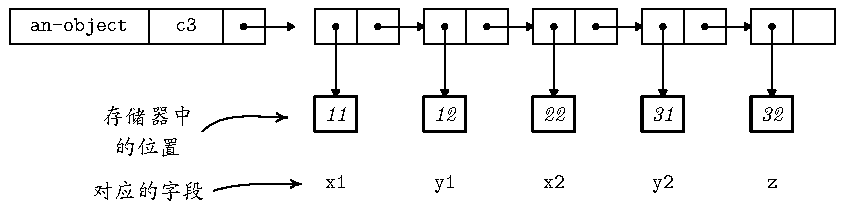
\includegraphics[scale=1.0]{simple-object.pdf}\end{SCentered}

\caption{简单对象\label{t:x28elem_x22figx2d9x2e9x22x29}}\end{EoplFigure}

\Ssubsubsection{对象}{对象}\label{t:x28part_x22s9x2e4x2e1x22x29}

\index{dzui4xiang4@对象|idxdecorator{}{}}
我们用包含类名和字段引用列表的数据类型表示对象。

\begin{EoplCodeInset}\begin{SCodeFlow}\begin{RktBlk}\begin{SingleColumn}\RktPn{(}\RktSym{define{-}datatype}\mbox{\hphantom{\Scribtexttt{x}}}\RktSym{object}\mbox{\hphantom{\Scribtexttt{x}}}\RktSym{object{\hbox{\texttt{?}}}}

\mbox{\hphantom{\Scribtexttt{xx}}}\RktPn{(}\RktSym{an{-}object}

\mbox{\hphantom{\Scribtexttt{xxxx}}}\RktPn{(}\RktSym{class{-}name}\mbox{\hphantom{\Scribtexttt{x}}}\RktSym{identifier{\hbox{\texttt{?}}}}\RktPn{)}

\mbox{\hphantom{\Scribtexttt{xxxx}}}\RktPn{(}\RktSym{fields}\mbox{\hphantom{\Scribtexttt{x}}}\RktPn{(}\RktSym{list{-}of}\mbox{\hphantom{\Scribtexttt{x}}}\RktSym{reference{\hbox{\texttt{?}}}}\RktPn{)}\RktPn{)}\RktPn{)}\RktPn{)}\end{SingleColumn}\end{RktBlk}\end{SCodeFlow}\end{EoplCodeInset}

在列表中,我们把“最年长”类的字段排在前面。这样,
在 中,类 \Scribtexttt{c1} 对象的字段排列为 \Scribtexttt{(x y)};类 \Scribtexttt{c2} 对
象的字段排列为 \Scribtexttt{(x y y)},其中,第二个 \Scribtexttt{y} 是 \Scribtexttt{c2} 中的;类 \Scribtexttt{c3} 对
象的字段排列为 \Scribtexttt{(x y y x z)}。 中对象 \Scribtexttt{o3} 的表示
如 所示。当然,我们想让类 \Scribtexttt{c3} 中的方法使用 \Scribtexttt{c3} 中声
明的字段 \Scribtexttt{x},而不是 \Scribtexttt{c1} 中声明的。在建立方法主体的求值环境时,我们要处理
这一点。

这种方法有个好处:对 \Scribtexttt{c3} 的任何子类,列表中的相同位置具有相同字段,因为后添
加的任何字段都会出现在这些字段的右边。在 \Scribtexttt{c3} 任一子类定义的某个方法中,
\Scribtexttt{x} 在什么位置呢?我们知道,如果没有重定义,\Scribtexttt{x} 在所有这些方法中的位置一定
是 3。这样,在声明字段变量时,变量对应值的位置保持不变。这一特点使字段引用的位置
能够静态地确定,就像我们在\SecRefLocal{t:x28part_x22s3x2e6x22x29}{3.6}{消除变量名}中处理变量那样。

\index{fzen1pei4@分配!dzui4xiang4@对象|idxdecorator{}{}}
创建新对象很容易。我们只需创建 \Scribtexttt{an{-}object},它有一个新引用列表,列表长度与对
象的字段数目相等。要确定其数目,我们从对象所属类中取出字段变量列表。我们用不合法
的值初始化所有位置,以便探知程序是否使用了未初始化的位置。

\begin{EoplCodeInset}\begin{SCodeFlow}\begin{RktBlk}\begin{SingleColumn}\texMathInline{\mathit{ClassName} = \mathit{Sym}}

\mbox{\hphantom{\Scribtexttt{x}}}

\textbf{\Scribtexttt{new{-}object}} : \texMathInline{\mathit{ClassName} \to \mathit{Obj}}

\RktPn{(}\RktSym{define}\mbox{\hphantom{\Scribtexttt{x}}}\RktSym{new{-}object}

\mbox{\hphantom{\Scribtexttt{xx}}}\RktPn{(}\RktSym{lambda}\mbox{\hphantom{\Scribtexttt{x}}}\RktPn{(}\RktSym{class{-}name}\RktPn{)}

\mbox{\hphantom{\Scribtexttt{xxxx}}}\RktPn{(}\RktSym{an{-}object}

\mbox{\hphantom{\Scribtexttt{xxxxxx}}}\RktSym{class{-}name}

\mbox{\hphantom{\Scribtexttt{xxxxxx}}}\RktPn{(}\RktSym{map}

\mbox{\hphantom{\Scribtexttt{xxxxxxxx}}}\RktPn{(}\RktSym{lambda}\mbox{\hphantom{\Scribtexttt{x}}}\RktPn{(}\RktSym{field{-}name}\RktPn{)}

\mbox{\hphantom{\Scribtexttt{xxxxxxxxxx}}}\RktPn{(}\RktSym{newref}\mbox{\hphantom{\Scribtexttt{x}}}\RktPn{(}\RktSym{list}\mbox{\hphantom{\Scribtexttt{x}}}\RktVal{{\textquotesingle}}\RktVal{uninitialized{-}field}\mbox{\hphantom{\Scribtexttt{x}}}\RktSym{field{-}name}\RktPn{)}\RktPn{)}\RktPn{)}

\mbox{\hphantom{\Scribtexttt{xxxxxxxx}}}\RktPn{(}\RktSym{class{-}{\Stttextmore}field{-}names}\mbox{\hphantom{\Scribtexttt{x}}}\RktPn{(}\RktSym{lookup{-}class}\mbox{\hphantom{\Scribtexttt{x}}}\RktSym{class{-}name}\RktPn{)}\RktPn{)}\RktPn{)}\RktPn{)}\RktPn{)}\RktPn{)}\end{SingleColumn}\end{RktBlk}\end{SCodeFlow}\end{EoplCodeInset}

\Ssubsubsection{方法}{方法}\label{t:x28part_x22s9x2e4x2e2x22x29}

\index{hzuan2jing4@环境!fzang1fa3diao4yong4@方法调用|(idxdecorator{}{}}
\index{dzui4xiang4zi4duan4@对象字段|(idxdecorator{}{}}
\index{dzui4xiang4cheng2yuan2@对象成员|(idxdecorator{}{}}
\index{mzian4xiang4dui4xiang4dexiao1xi1chuan2di4fang1fa3diao4yong4@面向对象的消息传递(方法调用)|(idxdecorator{}{}}
接下来我们处理方法。方法就像过程,但是它们不保存环境,而是记录所引用的字段名。方
法调用在如下环境中执行其主体:

\begin{itemize}\atItemizeStart

\item 方法的形参绑定到新引用,引用初始化为实参的值。这与 IMPLICIT{-}REFS 中的
\Scribtexttt{apply{-}procedure} 行为类似。

\item 伪变量 \Scribtexttt{\%self} 绑定到当前对象,\Scribtexttt{\%super} 绑定到当前方法的超类。
\index{wzei3bian4liang4@伪变量|idxdecorator{}{}}

\item 可见字段名绑定到当前对象的字段。要实现这点,我们定义

\begin{EoplCodeInset}\begin{SCodeFlow}\begin{RktBlk}\begin{SingleColumn}\RktPn{(}\RktSym{define{-}datatype}\mbox{\hphantom{\Scribtexttt{x}}}\RktSym{method}\mbox{\hphantom{\Scribtexttt{x}}}\RktSym{method{\hbox{\texttt{?}}}}

\mbox{\hphantom{\Scribtexttt{xx}}}\RktPn{(}\RktSym{a{-}method}

\mbox{\hphantom{\Scribtexttt{xxxx}}}\RktPn{(}\RktSym{vars}\mbox{\hphantom{\Scribtexttt{x}}}\RktPn{(}\RktSym{list{-}of}\mbox{\hphantom{\Scribtexttt{x}}}\RktSym{identifier{\hbox{\texttt{?}}}}\RktPn{)}\RktPn{)}

\mbox{\hphantom{\Scribtexttt{xxxx}}}\RktPn{(}\RktSym{body}\mbox{\hphantom{\Scribtexttt{x}}}\RktSym{expression{\hbox{\texttt{?}}}}\RktPn{)}

\mbox{\hphantom{\Scribtexttt{xxxx}}}\RktPn{(}\RktSym{super{-}name}\mbox{\hphantom{\Scribtexttt{x}}}\RktSym{identifier{\hbox{\texttt{?}}}}\RktPn{)}

\mbox{\hphantom{\Scribtexttt{xxxx}}}\RktPn{(}\RktSym{field{-}names}\mbox{\hphantom{\Scribtexttt{x}}}\RktPn{(}\RktSym{list{-}of}\mbox{\hphantom{\Scribtexttt{x}}}\RktSym{identifier{\hbox{\texttt{?}}}}\RktPn{)}\RktPn{)}\RktPn{)}\RktPn{)}

\mbox{\hphantom{\Scribtexttt{x}}}

\textbf{\Scribtexttt{apply{-}method}} : \texMathInline{\mathit{Method} \times \mathit{Obj} \times \mathit{Listof(ExpVal)} \to \mathit{ExpVal}}

\RktPn{(}\RktSym{define}\mbox{\hphantom{\Scribtexttt{x}}}\RktSym{apply{-}method}

\mbox{\hphantom{\Scribtexttt{xx}}}\RktPn{(}\RktSym{lambda}\mbox{\hphantom{\Scribtexttt{x}}}\RktPn{(}\RktSym{m}\mbox{\hphantom{\Scribtexttt{x}}}\RktSym{self}\mbox{\hphantom{\Scribtexttt{x}}}\RktSym{args}\RktPn{)}

\mbox{\hphantom{\Scribtexttt{xxxx}}}\RktPn{(}\RktSym{cases}\mbox{\hphantom{\Scribtexttt{x}}}\RktSym{method}\mbox{\hphantom{\Scribtexttt{x}}}\RktSym{m}

\mbox{\hphantom{\Scribtexttt{xxxxxx}}}\RktPn{(}\RktSym{a{-}method}\mbox{\hphantom{\Scribtexttt{x}}}\RktPn{(}\RktSym{vars}\mbox{\hphantom{\Scribtexttt{x}}}\RktSym{body}\mbox{\hphantom{\Scribtexttt{x}}}\RktSym{super{-}name}\mbox{\hphantom{\Scribtexttt{x}}}\RktSym{field{-}names}\RktPn{)}

\mbox{\hphantom{\Scribtexttt{xxxxxxxx}}}\RktPn{(}\RktSym{value{-}of}\mbox{\hphantom{\Scribtexttt{x}}}\RktSym{body}

\mbox{\hphantom{\Scribtexttt{xxxxxxxxxx}}}\RktPn{(}\RktSym{extend{-}env*}\mbox{\hphantom{\Scribtexttt{x}}}\RktSym{vars}\mbox{\hphantom{\Scribtexttt{x}}}\RktPn{(}\RktSym{map}\mbox{\hphantom{\Scribtexttt{x}}}\RktSym{newref}\mbox{\hphantom{\Scribtexttt{x}}}\RktSym{args}\RktPn{)}

\mbox{\hphantom{\Scribtexttt{xxxxxxxxxxxx}}}\RktPn{(}\RktSym{extend{-}env{-}with{-}self{-}and{-}super}

\mbox{\hphantom{\Scribtexttt{xxxxxxxxxxxxxx}}}\RktSym{self}\mbox{\hphantom{\Scribtexttt{x}}}\RktSym{super{-}name}

\mbox{\hphantom{\Scribtexttt{xxxxxxxxxxxxxx}}}\RktPn{(}\RktSym{extend{-}env*}\mbox{\hphantom{\Scribtexttt{x}}}\RktSym{field{-}names}\mbox{\hphantom{\Scribtexttt{x}}}\RktPn{(}\RktSym{object{-}{\Stttextmore}fields}\mbox{\hphantom{\Scribtexttt{x}}}\RktSym{self}\RktPn{)}

\mbox{\hphantom{\Scribtexttt{xxxxxxxxxxxxxxxx}}}\RktPn{(}\RktSym{empty{-}env}\RktPn{)}\RktPn{)}\RktPn{)}\RktPn{)}\RktPn{)}\RktPn{)}\RktPn{)}\RktPn{)}\RktPn{)}\end{SingleColumn}\end{RktBlk}\end{SCodeFlow}\end{EoplCodeInset}\end{itemize}

这里,我们使用ex2.10 中的 \Scribtexttt{extend{-}env*}。它在扩展环境时,把变
量列表绑定到指代值的列表。我们还给环境接口新增过程
\Scribtexttt{extend{-}env{-}with{-}self{-}and{-}super},分别将 \Scribtexttt{\%self} 和 \Scribtexttt{\%super} 绑定到对象
和类名。

要确保各方法看到正确的字段,我们在构建 \Scribtexttt{field{-}names} 列表时需要小心。各方法只
应见到最后一个声明的同名字段,其他同名字段应被遮蔽。所以,我们构建
\Scribtexttt{field{-}names} 列表时,把最右边之外的出现的每个重复名字替换为新名。
 中的程序对应的 \Scribtexttt{field{-}names} 如下

\begin{Subflow}\label{t:x28elem_x22fieldx2drenamingx22x29}

\noindent \begin{bigtabular}{@{\bigtableleftpad}l@{}l@{}l@{}l@{}l@{}l@{}l@{}}
\hbox{\textbf{类}} &
\hbox{\mbox{\hphantom{\Scribtexttt{xxxx}}}} &
\hbox{\textbf{定义的字段}} &
\hbox{\mbox{\hphantom{\Scribtexttt{xxxx}}}} &
\hbox{\textbf{字段}} &
\hbox{\mbox{\hphantom{\Scribtexttt{xxxx}}}} &
\hbox{\textbf{\Scribtexttt{field{-}names}}} \\
\hbox{\Scribtexttt{c1}} &
\hbox{\mbox{\hphantom{\Scribtexttt{xxxx}}}} &
\hbox{\Scribtexttt{x, y}} &
\hbox{\mbox{\hphantom{\Scribtexttt{xxxx}}}} &
\hbox{\Scribtexttt{(x y)}} &
\hbox{\mbox{\hphantom{\Scribtexttt{xxxx}}}} &
\hbox{\Scribtexttt{(x}\texMathInline{\phantom{xxx}}\Scribtexttt{y)}} \\
\hbox{\Scribtexttt{c2}} &
\hbox{\mbox{\hphantom{\Scribtexttt{xxxx}}}} &
\hbox{\Scribtexttt{y}} &
\hbox{\mbox{\hphantom{\Scribtexttt{xxxx}}}} &
\hbox{\Scribtexttt{(x y y)}} &
\hbox{\mbox{\hphantom{\Scribtexttt{xxxx}}}} &
\hbox{\Scribtexttt{(x}\texMathInline{\phantom{xxx}}\Scribtexttt{y\%1 y)}} \\
\hbox{\Scribtexttt{c3}} &
\hbox{\mbox{\hphantom{\Scribtexttt{xxxx}}}} &
\hbox{\Scribtexttt{x, z}} &
\hbox{\mbox{\hphantom{\Scribtexttt{xxxx}}}} &
\hbox{\Scribtexttt{(x y y x z)}} &
\hbox{\mbox{\hphantom{\Scribtexttt{xxxx}}}} &
\hbox{\Scribtexttt{(x\%1}\texMathInline{\phantom{x}}\Scribtexttt{y\%1 y x z)}}\end{bigtabular}

由于方法主体无从得知 \Scribtexttt{x\%1} 和 \Scribtexttt{y\%1},所以它们只能见到各字段变量在最右边的
声明,正合期望。\end{Subflow}

 展示的环境,是求 中 \Scribtexttt{send o3 m1(7,8)} 内方
法主体的值时创建的。这张图表明,引用列表可能比变量列表长:变量列表只是
\Scribtexttt{(x y\%1 y)},因为 \Scribtexttt{c2} 的方法 \Scribtexttt{m1} 只能见到这些字段变量,但
\Scribtexttt{(object{-}{\Stttextmore}fields self)} 的值是对象中所有字段的列表。不过,由于三个可见字段变
量的值是列表中的头三个元素,而且我们把第一个 \Scribtexttt{y} 重命名为 \Scribtexttt{y\%1}(该方法对
此一无所知),方法 \Scribtexttt{m1} 将把变量 \Scribtexttt{y} 与 \Scribtexttt{c2} 中声明的 \Scribtexttt{y} 关联起来,
正合期望。

\begin{EoplFigure}[!t]

\noindent \begin{SCentered}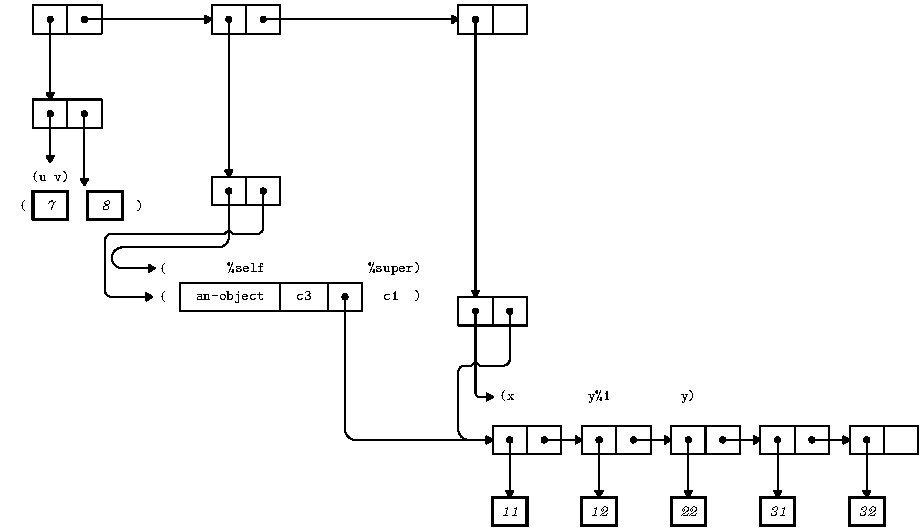
\includegraphics[scale=1.0]{env-for-method.pdf}\end{SCentered}

\index{extendenvasterisk@\textbf{\Scribtexttt{extend{-}env*}}|idxdecorator{}{}}


\noindent \caption{方法调用时的环境\label{t:x28elem_x22figx2d9x2e10x22x29}}\end{EoplFigure}

\index{self@\Scribtexttt{self}|idxdecorator{}{}}
当 \Scribtexttt{self} 的持有类和所属类相同时,变量列表的长度通常与字段引用列表相同。如果
持有类位于类链的上端,那么位置数可能多于字段变量数目,但对应于字段变量的值位于列
表开头,其余值则不可见。\index{czhi2you3lei4@持有类|idxdecorator{}{}}
\index{hzuan2jing4@环境!fzang1fa3diao4yong4@方法调用|)idxdecorator{}{}}
\index{dzui4xiang4zi4duan4@对象字段|)idxdecorator{}{}}
\index{dzui4xiang4cheng2yuan2@对象成员|)idxdecorator{}{}}
\index{mzian4xiang4dui4xiang4dexiao1xi1chuan2di4fang1fa3diao4yong4@面向对象的消息传递(方法调用)|)idxdecorator{}{}}

\Ssubsubsection{类和类环境}{类和类环境}\label{t:x28part_x22s9x2e4x2e3x22x29}

\index{lzei4huan2jing4@类环境|(idxdecorator{}{}}
\index{lzei4@类|(idxdecorator{}{}}
\index{lzei4@类!czhi2you3lei4@持有类|idxdecorator{}{}}
\index{hzuan2jing4@环境!lzei4huan2jing4@类环境|(idxdecorator{}{}}
迄今为止,我们的实现都依赖从类名获取与类相关的信息。所以,我们需要
一个\emph{类环境} (\emph{class environment}) 完成这一工作。类环境将每个类名与描述类的
数据结构关联起来。

类环境是全局的:在我们的语言中,类声明聚集于程序开头,且对整个程序生效。所以,我
们用名为 \Scribtexttt{the{-}class{-}env} 的全局变量表示类环境,它包含列表 \Scribtexttt{(类名,类)} 的列
表,但我们用过程 \Scribtexttt{add{-}to{-}class{-}env{\hbox{\texttt{!}}}} 和 \Scribtexttt{lookup{-}class} 隐藏这一表示。

\begin{EoplCodeInset}\begin{SCodeFlow}\begin{RktBlk}\begin{SingleColumn}\texMathInline{\mathit{ClassEnv} = \mathit{Listof(List(ClassName, Class))}}

\mbox{\hphantom{\Scribtexttt{x}}}

\textbf{\Scribtexttt{the{-}class{-}env}} : \texMathInline{\mathit{ClassEnv}}

\RktPn{(}\RktSym{define}\mbox{\hphantom{\Scribtexttt{x}}}\RktSym{the{-}class{-}env}\mbox{\hphantom{\Scribtexttt{x}}}\RktVal{{\textquotesingle}}\RktVal{(}\RktVal{)}\RktPn{)}

\mbox{\hphantom{\Scribtexttt{x}}}

\textbf{\Scribtexttt{add{-}to{-}class{-}env{\hbox{\texttt{!}}}}} : \texMathInline{\mathit{ClassName} \times \mathit{Class} \to \mathit{Unspecified}}

\RktPn{(}\RktSym{define}\mbox{\hphantom{\Scribtexttt{x}}}\RktSym{add{-}to{-}class{-}env{\hbox{\texttt{!}}}}

\mbox{\hphantom{\Scribtexttt{xx}}}\RktPn{(}\RktSym{lambda}\mbox{\hphantom{\Scribtexttt{x}}}\RktPn{(}\RktSym{class{-}name}\mbox{\hphantom{\Scribtexttt{x}}}\RktSym{class}\RktPn{)}

\mbox{\hphantom{\Scribtexttt{xxxx}}}\RktPn{(}\RktSym{set{\hbox{\texttt{!}}}}\mbox{\hphantom{\Scribtexttt{x}}}\RktSym{the{-}class{-}env}

\mbox{\hphantom{\Scribtexttt{xxxxxx}}}\RktPn{(}\RktSym{cons}

\mbox{\hphantom{\Scribtexttt{xxxxxxxx}}}\RktPn{(}\RktSym{list}\mbox{\hphantom{\Scribtexttt{x}}}\RktSym{class{-}name}\mbox{\hphantom{\Scribtexttt{x}}}\RktSym{class}\RktPn{)}

\mbox{\hphantom{\Scribtexttt{xxxxxxxx}}}\RktSym{the{-}class{-}env}\RktPn{)}\RktPn{)}\RktPn{)}\RktPn{)}

\mbox{\hphantom{\Scribtexttt{x}}}

\textbf{\Scribtexttt{lookup{-}class}} : \texMathInline{\mathit{ClassName} \to \mathit{Class}}

\RktPn{(}\RktSym{define}\mbox{\hphantom{\Scribtexttt{x}}}\RktSym{lookup{-}class}

\mbox{\hphantom{\Scribtexttt{xx}}}\RktPn{(}\RktSym{lambda}\mbox{\hphantom{\Scribtexttt{x}}}\RktPn{(}\RktSym{name}\RktPn{)}

\mbox{\hphantom{\Scribtexttt{xxxx}}}\RktPn{(}\RktSym{let}\mbox{\hphantom{\Scribtexttt{x}}}\RktPn{(}\RktPn{(}\RktSym{maybe{-}pair}\mbox{\hphantom{\Scribtexttt{x}}}\RktPn{(}\RktSym{assq}\mbox{\hphantom{\Scribtexttt{x}}}\RktSym{name}\mbox{\hphantom{\Scribtexttt{x}}}\RktSym{the{-}class{-}env}\RktPn{)}\RktPn{)}\RktPn{)}

\mbox{\hphantom{\Scribtexttt{xxxxxx}}}\RktPn{(}\RktSym{if}\mbox{\hphantom{\Scribtexttt{x}}}\RktSym{maybe{-}pair}\mbox{\hphantom{\Scribtexttt{x}}}\RktPn{(}\RktSym{cadr}\mbox{\hphantom{\Scribtexttt{x}}}\RktSym{maybe{-}pair}\RktPn{)}

\mbox{\hphantom{\Scribtexttt{xxxxxxxx}}}\RktPn{(}\RktSym{report{-}unknown{-}class}\mbox{\hphantom{\Scribtexttt{x}}}\RktSym{name}\RktPn{)}\RktPn{)}\RktPn{)}\RktPn{)}\RktPn{)}\end{SingleColumn}\end{RktBlk}\end{SCodeFlow}\end{EoplCodeInset}

对每个类,我们记录三样东西:超类的名字,字段变量的列表,以及将方法名映射到方法的
环境。

\begin{Subflow}\begin{EoplCodeInset}\begin{SCodeFlow}\begin{RktBlk}\begin{SingleColumn}\RktPn{(}\RktSym{define{-}datatype}\mbox{\hphantom{\Scribtexttt{x}}}\RktSym{class}\mbox{\hphantom{\Scribtexttt{x}}}\RktSym{class{\hbox{\texttt{?}}}}

\mbox{\hphantom{\Scribtexttt{xx}}}\RktPn{(}\RktSym{a{-}class}

\mbox{\hphantom{\Scribtexttt{xxxx}}}\RktPn{(}\RktSym{super{-}name}\mbox{\hphantom{\Scribtexttt{x}}}\RktPn{(}\RktSym{maybe}\mbox{\hphantom{\Scribtexttt{x}}}\RktSym{identifier{\hbox{\texttt{?}}}}\RktPn{)}\RktPn{)}

\mbox{\hphantom{\Scribtexttt{xxxx}}}\RktPn{(}\RktSym{field{-}names}\mbox{\hphantom{\Scribtexttt{x}}}\RktPn{(}\RktSym{list{-}of}\mbox{\hphantom{\Scribtexttt{x}}}\RktSym{identifier{\hbox{\texttt{?}}}}\RktPn{)}\RktPn{)}

\mbox{\hphantom{\Scribtexttt{xxxx}}}\RktPn{(}\RktSym{method{-}env}\mbox{\hphantom{\Scribtexttt{x}}}\RktSym{method{-}environment{\hbox{\texttt{?}}}}\RktPn{)}\RktPn{)}\RktPn{)}\end{SingleColumn}\end{RktBlk}\end{SCodeFlow}\end{EoplCodeInset}

这里,我们用谓词 \Scribtexttt{(maybe identifier{\hbox{\texttt{?}}})} 判断值是否为符号或 \Scribtexttt{\#f}。后一种情况
对是必须的,因为类 \Scribtexttt{object} 没有超类。\Scribtexttt{filed{-}names} 是类的方法能见到的字段,
\Scribtexttt{method{-}env} 是一环境,给出了类中每个方法名的定义。\end{Subflow}

我们初始化类环境时,为类 \Scribtexttt{object} 添加一个绑定。对每个声明,我们向类环境添加
一个新绑定,将类名绑定到一个 \Scribtexttt{class},它包含超类名、类中方法的
\Scribtexttt{field{-}names} 以及类中方法的环境。

\begin{EoplCodeInset}\begin{SCodeFlow}\begin{RktBlk}\begin{SingleColumn}\label{t:x28elem_x22initializex2dclassx2denvx21x22x29}\textbf{\Scribtexttt{initialize{-}class{-}env{\hbox{\texttt{!}}}}} : \texMathInline{\mathit{Listof(ClassDecl)} \to \mathit{Unspecified}}

\RktPn{(}\RktSym{define}\mbox{\hphantom{\Scribtexttt{x}}}\RktSym{initialize{-}class{-}env{\hbox{\texttt{!}}}}

\mbox{\hphantom{\Scribtexttt{xx}}}\RktPn{(}\RktSym{lambda}\mbox{\hphantom{\Scribtexttt{x}}}\RktPn{(}\RktSym{c{-}decls}\RktPn{)}

\mbox{\hphantom{\Scribtexttt{xxxx}}}\RktPn{(}\RktSym{set{\hbox{\texttt{!}}}}\mbox{\hphantom{\Scribtexttt{x}}}\RktSym{the{-}class{-}env}

\mbox{\hphantom{\Scribtexttt{xxxxxx}}}\RktPn{(}\RktSym{list}

\mbox{\hphantom{\Scribtexttt{xxxxxxxx}}}\RktPn{(}\RktSym{list}\mbox{\hphantom{\Scribtexttt{x}}}\RktVal{{\textquotesingle}}\RktVal{object}\mbox{\hphantom{\Scribtexttt{x}}}\RktPn{(}\RktSym{a{-}class}\mbox{\hphantom{\Scribtexttt{x}}}\RktVal{\#f}\mbox{\hphantom{\Scribtexttt{x}}}\RktVal{{\textquotesingle}}\RktVal{(}\RktVal{)}\mbox{\hphantom{\Scribtexttt{x}}}\RktVal{{\textquotesingle}}\RktVal{(}\RktVal{)}\RktPn{)}\RktPn{)}\RktPn{)}\RktPn{)}

\mbox{\hphantom{\Scribtexttt{xxxx}}}\RktPn{(}\RktSym{for{-}each}\mbox{\hphantom{\Scribtexttt{x}}}\RktSym{initialize{-}class{-}decl{\hbox{\texttt{!}}}}\mbox{\hphantom{\Scribtexttt{x}}}\RktSym{c{-}decls}\RktPn{)}\RktPn{)}\RktPn{)}

\mbox{\hphantom{\Scribtexttt{x}}}

\textbf{\Scribtexttt{initialize{-}class{-}decl{\hbox{\texttt{!}}}}} : \texMathInline{\mathit{ClassDecl} \to \mathit{Unspecified}}

\RktPn{(}\RktSym{define}\mbox{\hphantom{\Scribtexttt{x}}}\RktSym{initialize{-}class{-}decl{\hbox{\texttt{!}}}}

\mbox{\hphantom{\Scribtexttt{xx}}}\RktPn{(}\RktSym{lambda}\mbox{\hphantom{\Scribtexttt{x}}}\RktPn{(}\RktSym{c{-}decl}\RktPn{)}

\mbox{\hphantom{\Scribtexttt{xxxx}}}\RktPn{(}\RktSym{cases}\mbox{\hphantom{\Scribtexttt{x}}}\RktSym{class{-}decl}\mbox{\hphantom{\Scribtexttt{x}}}\RktSym{c{-}decl}

\mbox{\hphantom{\Scribtexttt{xxxxxx}}}\RktPn{(}\RktSym{a{-}class{-}decl}\mbox{\hphantom{\Scribtexttt{x}}}\RktPn{(}\RktSym{c{-}name}\mbox{\hphantom{\Scribtexttt{x}}}\RktSym{s{-}name}\mbox{\hphantom{\Scribtexttt{x}}}\RktSym{f{-}names}\mbox{\hphantom{\Scribtexttt{x}}}\RktSym{m{-}decls}\RktPn{)}

\mbox{\hphantom{\Scribtexttt{xxxxxxxx}}}\RktPn{(}\RktSym{let}\mbox{\hphantom{\Scribtexttt{x}}}\RktPn{(}\RktPn{(}\RktSym{f{-}names}

\mbox{\hphantom{\Scribtexttt{xxxxxxxxxxxxxxxx}}}\RktPn{(}\RktSym{append{-}field{-}names}

\mbox{\hphantom{\Scribtexttt{xxxxxxxxxxxxxxxxxx}}}\RktPn{(}\RktSym{class{-}{\Stttextmore}field{-}names}\mbox{\hphantom{\Scribtexttt{x}}}\RktPn{(}\RktSym{lookup{-}class}\mbox{\hphantom{\Scribtexttt{x}}}\RktSym{s{-}name}\RktPn{)}\RktPn{)}

\mbox{\hphantom{\Scribtexttt{xxxxxxxxxxxxxxxxxx}}}\RktSym{f{-}names}\RktPn{)}\RktPn{)}\RktPn{)}

\mbox{\hphantom{\Scribtexttt{xxxxxxxxxx}}}\RktPn{(}\RktSym{add{-}to{-}class{-}env{\hbox{\texttt{!}}}}

\mbox{\hphantom{\Scribtexttt{xxxxxxxxxxxx}}}\RktSym{c{-}name}

\mbox{\hphantom{\Scribtexttt{xxxxxxxxxxxx}}}\RktPn{(}\RktSym{a{-}class}\mbox{\hphantom{\Scribtexttt{x}}}\RktSym{s{-}name}\mbox{\hphantom{\Scribtexttt{x}}}\RktSym{f{-}names}

\mbox{\hphantom{\Scribtexttt{xxxxxxxxxxxxxx}}}\RktPn{(}\RktSym{merge{-}method{-}envs}

\mbox{\hphantom{\Scribtexttt{xxxxxxxxxxxxxxxx}}}\RktPn{(}\RktSym{class{-}{\Stttextmore}method{-}env}\mbox{\hphantom{\Scribtexttt{x}}}\RktPn{(}\RktSym{lookup{-}class}\mbox{\hphantom{\Scribtexttt{x}}}\RktSym{s{-}name}\RktPn{)}\RktPn{)}

\mbox{\hphantom{\Scribtexttt{xxxxxxxxxxxxxxxx}}}\RktPn{(}\RktSym{method{-}decls{-}{\Stttextmore}method{-}env}

\mbox{\hphantom{\Scribtexttt{xxxxxxxxxxxxxxxxxx}}}\RktSym{m{-}decls}\mbox{\hphantom{\Scribtexttt{x}}}\RktSym{s{-}name}\mbox{\hphantom{\Scribtexttt{x}}}\RktSym{f{-}names}\RktPn{)}\RktPn{)}\RktPn{)}\RktPn{)}\RktPn{)}\RktPn{)}\RktPn{)}\RktPn{)}\RktPn{)}\end{SingleColumn}\end{RktBlk}\end{SCodeFlow}\end{EoplCodeInset}

过程 \Scribtexttt{append{-}field{-}names} 用来给当前类创建 \Scribtexttt{field{-}names}。它将新类声明的字
段添加到超类字段之后,同时将超类中被新字段遮蔽的字段替换为新名字,
就像field{-}renaming的示例那样。

\begin{EoplCodeInset}\begin{SCodeFlow}\begin{RktBlk}\begin{SingleColumn}\textbf{\Scribtexttt{append{-}field{-}names}} : \hspace*{\fill}\\\texMathInline{\phantom{xx}}\texMathInline{\mathit{Listof(FieldName)} \times \mathit{Listof(FieldName)} \to \mathit{Listof(FieldName)}}

\RktPn{(}\RktSym{define}\mbox{\hphantom{\Scribtexttt{x}}}\RktSym{append{-}field{-}names}

\mbox{\hphantom{\Scribtexttt{xx}}}\RktPn{(}\RktSym{lambda}\mbox{\hphantom{\Scribtexttt{x}}}\RktPn{(}\RktSym{super{-}fields}\mbox{\hphantom{\Scribtexttt{x}}}\RktSym{new{-}fields}\RktPn{)}

\mbox{\hphantom{\Scribtexttt{xxxx}}}\RktPn{(}\RktSym{cond}

\mbox{\hphantom{\Scribtexttt{xxxxxx}}}\RktPn{(}\RktPn{(}\RktSym{null{\hbox{\texttt{?}}}}\mbox{\hphantom{\Scribtexttt{x}}}\RktSym{super{-}fields}\RktPn{)}\mbox{\hphantom{\Scribtexttt{x}}}\RktSym{new{-}fields}\RktPn{)}

\mbox{\hphantom{\Scribtexttt{xxxxxx}}}\RktPn{(}\RktSym{else}

\mbox{\hphantom{\Scribtexttt{xxxxxxxx}}}\RktPn{(}\RktSym{cons}

\mbox{\hphantom{\Scribtexttt{xxxxxxxxxx}}}\RktPn{(}\RktSym{if}\mbox{\hphantom{\Scribtexttt{x}}}\RktPn{(}\RktSym{memq}\mbox{\hphantom{\Scribtexttt{x}}}\RktPn{(}\RktSym{car}\mbox{\hphantom{\Scribtexttt{x}}}\RktSym{super{-}fields}\RktPn{)}\mbox{\hphantom{\Scribtexttt{x}}}\RktSym{new{-}fields}\RktPn{)}

\mbox{\hphantom{\Scribtexttt{xxxxxxxxxxxx}}}\RktPn{(}\RktSym{fresh{-}identifier}\mbox{\hphantom{\Scribtexttt{x}}}\RktPn{(}\RktSym{car}\mbox{\hphantom{\Scribtexttt{x}}}\RktSym{super{-}fields}\RktPn{)}\RktPn{)}

\mbox{\hphantom{\Scribtexttt{xxxxxxxxxxxx}}}\RktPn{(}\RktSym{car}\mbox{\hphantom{\Scribtexttt{x}}}\RktSym{super{-}fields}\RktPn{)}\RktPn{)}

\mbox{\hphantom{\Scribtexttt{xxxxxxxxxx}}}\RktPn{(}\RktSym{append{-}field{-}names}

\mbox{\hphantom{\Scribtexttt{xxxxxxxxxxxx}}}\RktPn{(}\RktSym{cdr}\mbox{\hphantom{\Scribtexttt{x}}}\RktSym{super{-}fields}\RktPn{)}\mbox{\hphantom{\Scribtexttt{x}}}\RktSym{new{-}fields}\RktPn{)}\RktPn{)}\RktPn{)}\RktPn{)}\RktPn{)}\RktPn{)}\end{SingleColumn}\end{RktBlk}\end{SCodeFlow}\end{EoplCodeInset}

\noindent \index{lzei4huan2jing4@类环境|)idxdecorator{}{}}
\index{lzei4@类|)idxdecorator{}{}}
\index{hzuan2jing4@环境!lzei4huan2jing4@类环境|)idxdecorator{}{}}

\Ssubsubsection{方法环境}{方法环境}\label{t:x28part_x22s9x2e4x2e4x22x29}

\index{hzuan2jing4@环境!fzang1fa3huan2jing4@方法环境|(idxdecorator{}{}}
\index{fzang1fa3huan2jing4@方法环境|(idxdecorator{}{}}
剩下的只有 \Scribtexttt{find{-}method} 和 \Scribtexttt{merge{-}method{-}envs} 了。

像处理类那样,我们用列表 \Scribtexttt{(方法名,方法)} 的列表表示方法环境,用
\Scribtexttt{find{-}method} 查找方法。

\begin{EoplCodeInset}\begin{SCodeFlow}\begin{RktBlk}\begin{SingleColumn}\texMathInline{\mathit{MethodEnv} = \mathit{Listof(List(MethodName, Method))}}

\mbox{\hphantom{\Scribtexttt{x}}}

\textbf{\Scribtexttt{find{-}method}} : \texMathInline{\mathit{Sym} \times \mathit{Sym} \to \mathit{Method}}

\RktPn{(}\RktSym{define}\mbox{\hphantom{\Scribtexttt{x}}}\RktSym{find{-}method}

\mbox{\hphantom{\Scribtexttt{xx}}}\RktPn{(}\RktSym{lambda}\mbox{\hphantom{\Scribtexttt{x}}}\RktPn{(}\RktSym{c{-}name}\mbox{\hphantom{\Scribtexttt{x}}}\RktSym{name}\RktPn{)}

\mbox{\hphantom{\Scribtexttt{xxxx}}}\RktPn{(}\RktSym{let}\mbox{\hphantom{\Scribtexttt{x}}}\RktPn{(}\RktPn{(}\RktSym{m{-}env}\mbox{\hphantom{\Scribtexttt{x}}}\RktPn{(}\RktSym{class{-}{\Stttextmore}method{-}env}\mbox{\hphantom{\Scribtexttt{x}}}\RktPn{(}\RktSym{lookup{-}class}\mbox{\hphantom{\Scribtexttt{x}}}\RktSym{c{-}name}\RktPn{)}\RktPn{)}\RktPn{)}\RktPn{)}

\mbox{\hphantom{\Scribtexttt{xxxxxx}}}\RktPn{(}\RktSym{let}\mbox{\hphantom{\Scribtexttt{x}}}\RktPn{(}\RktPn{(}\RktSym{maybe{-}pair}\mbox{\hphantom{\Scribtexttt{x}}}\RktPn{(}\RktSym{assq}\mbox{\hphantom{\Scribtexttt{x}}}\RktSym{name}\mbox{\hphantom{\Scribtexttt{x}}}\RktSym{m{-}env}\RktPn{)}\RktPn{)}\RktPn{)}

\mbox{\hphantom{\Scribtexttt{xxxxxxxx}}}\RktPn{(}\RktSym{if}\mbox{\hphantom{\Scribtexttt{x}}}\RktPn{(}\RktSym{pair{\hbox{\texttt{?}}}}\mbox{\hphantom{\Scribtexttt{x}}}\RktSym{maybe{-}pair}\RktPn{)}\mbox{\hphantom{\Scribtexttt{x}}}\RktPn{(}\RktSym{cadr}\mbox{\hphantom{\Scribtexttt{x}}}\RktSym{maybe{-}pair}\RktPn{)}

\mbox{\hphantom{\Scribtexttt{xxxxxxxxxx}}}\RktPn{(}\RktSym{report{-}method{-}not{-}found}\mbox{\hphantom{\Scribtexttt{x}}}\RktSym{name}\RktPn{)}\RktPn{)}\RktPn{)}\RktPn{)}\RktPn{)}\RktPn{)}\end{SingleColumn}\end{RktBlk}\end{SCodeFlow}\end{EoplCodeInset}

用这一信息,我们可以写出 \Scribtexttt{method{-}decls{-}{\Stttextmore}method{-}env}。它取一个类的方法声明,创
建一个方法环境,记录每个方法的绑定变量、主体、持有类的超类名,以及持有类的
\Scribtexttt{field{-}names}。

\begin{EoplCodeInset}\begin{SCodeFlow}\begin{RktBlk}\begin{SingleColumn}\textbf{\Scribtexttt{method{-}decls{-}{\Stttextmore}method{-}env}} : \hspace*{\fill}\\\texMathInline{\phantom{xx}}\texMathInline{\mathit{Listof(MethodDecl)} \times \mathit{ClassName} \times \mathit{Listof(FieldName)} \to \mathit{MethodEnv}}

\RktPn{(}\RktSym{define}\mbox{\hphantom{\Scribtexttt{x}}}\RktSym{method{-}decls{-}{\Stttextmore}method{-}env}

\mbox{\hphantom{\Scribtexttt{xx}}}\RktPn{(}\RktSym{lambda}\mbox{\hphantom{\Scribtexttt{x}}}\RktPn{(}\RktSym{m{-}decls}\mbox{\hphantom{\Scribtexttt{x}}}\RktSym{super{-}name}\mbox{\hphantom{\Scribtexttt{x}}}\RktSym{field{-}names}\RktPn{)}

\mbox{\hphantom{\Scribtexttt{xxxx}}}\RktPn{(}\RktSym{map}

\mbox{\hphantom{\Scribtexttt{xxxxxx}}}\RktPn{(}\RktSym{lambda}\mbox{\hphantom{\Scribtexttt{x}}}\RktPn{(}\RktSym{m{-}decl}\RktPn{)}

\mbox{\hphantom{\Scribtexttt{xxxxxxxx}}}\RktPn{(}\RktSym{cases}\mbox{\hphantom{\Scribtexttt{x}}}\RktSym{method{-}decl}\mbox{\hphantom{\Scribtexttt{x}}}\RktSym{m{-}decl}

\mbox{\hphantom{\Scribtexttt{xxxxxxxxxx}}}\RktPn{(}\RktSym{a{-}method{-}decl}\mbox{\hphantom{\Scribtexttt{x}}}\RktPn{(}\RktSym{method{-}name}\mbox{\hphantom{\Scribtexttt{x}}}\RktSym{vars}\mbox{\hphantom{\Scribtexttt{x}}}\RktSym{body}\RktPn{)}

\mbox{\hphantom{\Scribtexttt{xxxxxxxxxxxx}}}\RktPn{(}\RktSym{list}\mbox{\hphantom{\Scribtexttt{x}}}\RktSym{method{-}name}

\mbox{\hphantom{\Scribtexttt{xxxxxxxxxxxxxx}}}\RktPn{(}\RktSym{a{-}method}\mbox{\hphantom{\Scribtexttt{x}}}\RktSym{vars}\mbox{\hphantom{\Scribtexttt{x}}}\RktSym{body}\mbox{\hphantom{\Scribtexttt{x}}}\RktSym{super{-}name}\mbox{\hphantom{\Scribtexttt{x}}}\RktSym{field{-}names}\RktPn{)}\RktPn{)}\RktPn{)}\RktPn{)}\RktPn{)}

\mbox{\hphantom{\Scribtexttt{xxxxxx}}}\RktSym{m{-}decls}\RktPn{)}\RktPn{)}\RktPn{)}\end{SingleColumn}\end{RktBlk}\end{SCodeFlow}\end{EoplCodeInset}

最后,我们写出 \Scribtexttt{merge{-}method{-}envs}。由于新类中的方法覆盖了旧类的同名方法,我
们可以直接扩展环境,将新方法添加到前面。

\begin{Subflow}\begin{EoplCodeInset}\begin{SCodeFlow}\begin{RktBlk}\begin{SingleColumn}\textbf{\Scribtexttt{merge{-}method{-}envs}} : \texMathInline{\mathit{MethodEnv} \times \mathit{MethodEnv} \to \mathit{MethodEnv}}

\RktPn{(}\RktSym{define}\mbox{\hphantom{\Scribtexttt{x}}}\RktSym{merge{-}method{-}envs}

\mbox{\hphantom{\Scribtexttt{xx}}}\RktPn{(}\RktSym{lambda}\mbox{\hphantom{\Scribtexttt{x}}}\RktPn{(}\RktSym{super{-}m{-}env}\mbox{\hphantom{\Scribtexttt{x}}}\RktSym{new{-}m{-}env}\RktPn{)}

\mbox{\hphantom{\Scribtexttt{xxxx}}}\RktPn{(}\RktSym{append}\mbox{\hphantom{\Scribtexttt{x}}}\RktSym{new{-}m{-}env}\mbox{\hphantom{\Scribtexttt{x}}}\RktSym{super{-}m{-}env}\RktPn{)}\RktPn{)}\RktPn{)}\end{SingleColumn}\end{RktBlk}\end{SCodeFlow}\end{EoplCodeInset}

构建方法环境还有其他一些方式,它们在方法查询时更高效(ex9.18)。\end{Subflow}

\noindent \index{hzuan2jing4@环境!fzang1fa3huan2jing4@方法环境|)idxdecorator{}{}}
\index{fzang1fa3huan2jing4@方法环境|)idxdecorator{}{}}
\index{valueof@\textbf{\Scribtexttt{value{-}of}}!CLASSES@CLASSES|)idxdecorator{}{}}

\begin{EoplFigure}\begin{SCodeFlow}\begin{RktBlk}\begin{SingleColumn}\RktPn{(}\RktPn{(}\RktSym{c3}

\mbox{\hphantom{\Scribtexttt{xxx}}}\RktVal{\#}\RktVal{(}\RktVal{struct{\hbox{\texttt{:}}}a{-}class}\mbox{\hphantom{\Scribtexttt{x}}}\RktVal{c2}\mbox{\hphantom{\Scribtexttt{x}}}\RktVal{(}\RktVal{x\%2}\mbox{\hphantom{\Scribtexttt{x}}}\RktVal{y\%1}\mbox{\hphantom{\Scribtexttt{x}}}\RktVal{y}\mbox{\hphantom{\Scribtexttt{x}}}\RktVal{x}\mbox{\hphantom{\Scribtexttt{x}}}\RktVal{z}\RktVal{)}

\mbox{\hphantom{\Scribtexttt{xxxxxx}}}\RktVal{(}\RktVal{(}\RktVal{initialize}\mbox{\hphantom{\Scribtexttt{x}}}\RktVal{\#}\RktVal{(}\RktVal{struct{\hbox{\texttt{:}}}a{-}method}\mbox{\hphantom{\Scribtexttt{x}}}\RktVal{(}\RktVal{)}

\mbox{\hphantom{\Scribtexttt{xxxxxxxxxxxxxxxxxxxxxx}}}\RktVal{\#}\RktVal{(}\RktVal{struct{\hbox{\texttt{:}}}begin{-}exp}\mbox{\hphantom{\Scribtexttt{x}}}\RktVal{{\hbox{\texttt{.}}}{\hbox{\texttt{.}}}{\hbox{\texttt{.}}}}\RktVal{)}\mbox{\hphantom{\Scribtexttt{x}}}\RktVal{c2}\mbox{\hphantom{\Scribtexttt{x}}}\RktVal{(}\RktVal{x\%2}\mbox{\hphantom{\Scribtexttt{x}}}\RktVal{y\%1}\mbox{\hphantom{\Scribtexttt{x}}}\RktVal{y}\mbox{\hphantom{\Scribtexttt{x}}}\RktVal{x}\mbox{\hphantom{\Scribtexttt{x}}}\RktVal{z}\RktVal{)}\RktVal{)}\RktVal{)}

\mbox{\hphantom{\Scribtexttt{xxxxxxxx}}}\RktVal{(}\RktVal{m3}\mbox{\hphantom{\Scribtexttt{x}}}\RktVal{\#}\RktVal{(}\RktVal{struct{\hbox{\texttt{:}}}a{-}method}\mbox{\hphantom{\Scribtexttt{x}}}\RktVal{(}\RktVal{)}

\mbox{\hphantom{\Scribtexttt{xxxxxxxxxxxxxxx}}}\RktVal{\#}\RktVal{(}\RktVal{struct{\hbox{\texttt{:}}}diff{-}exp}\mbox{\hphantom{\Scribtexttt{x}}}\RktVal{{\hbox{\texttt{.}}}{\hbox{\texttt{.}}}{\hbox{\texttt{.}}}}\RktVal{)}\RktVal{)}\mbox{\hphantom{\Scribtexttt{x}}}\RktVal{c2}\mbox{\hphantom{\Scribtexttt{x}}}\RktVal{(}\RktVal{x\%2}\mbox{\hphantom{\Scribtexttt{x}}}\RktVal{y\%1}\mbox{\hphantom{\Scribtexttt{x}}}\RktVal{y}\mbox{\hphantom{\Scribtexttt{x}}}\RktVal{x}\mbox{\hphantom{\Scribtexttt{x}}}\RktVal{z}\RktVal{)}\RktVal{)}

\mbox{\hphantom{\Scribtexttt{xxxxxxxx}}}\RktVal{(}\RktVal{initialize}\mbox{\hphantom{\Scribtexttt{x}}}\RktVal{\#}\RktVal{(}\RktVal{struct{\hbox{\texttt{:}}}a{-}method}\mbox{\hphantom{\Scribtexttt{x}}}\RktVal{{\hbox{\texttt{.}}}{\hbox{\texttt{.}}}{\hbox{\texttt{.}}}}\RktVal{)}\RktVal{)}

\mbox{\hphantom{\Scribtexttt{xxxxxxxx}}}\RktVal{(}\RktVal{m1}\mbox{\hphantom{\Scribtexttt{x}}}\RktVal{\#}\RktVal{(}\RktVal{struct{\hbox{\texttt{:}}}a{-}method}\mbox{\hphantom{\Scribtexttt{x}}}\RktVal{(}\RktVal{u}\mbox{\hphantom{\Scribtexttt{x}}}\RktVal{v}\RktVal{)}

\mbox{\hphantom{\Scribtexttt{xxxxxxxxxxxxxxx}}}\RktVal{\#}\RktVal{(}\RktVal{struct{\hbox{\texttt{:}}}diff{-}exp}\mbox{\hphantom{\Scribtexttt{x}}}\RktVal{{\hbox{\texttt{.}}}{\hbox{\texttt{.}}}{\hbox{\texttt{.}}}}\RktVal{)}\mbox{\hphantom{\Scribtexttt{x}}}\RktVal{c1}\mbox{\hphantom{\Scribtexttt{x}}}\RktVal{(}\RktVal{x}\mbox{\hphantom{\Scribtexttt{x}}}\RktVal{y\%1}\mbox{\hphantom{\Scribtexttt{x}}}\RktVal{y}\RktVal{)}\RktVal{)}\RktVal{)}

\mbox{\hphantom{\Scribtexttt{xxxxxxxx}}}\RktVal{(}\RktVal{m3}\mbox{\hphantom{\Scribtexttt{x}}}\RktVal{\#}\RktVal{(}\RktVal{struct{\hbox{\texttt{:}}}a{-}method}\mbox{\hphantom{\Scribtexttt{x}}}\RktVal{{\hbox{\texttt{.}}}{\hbox{\texttt{.}}}{\hbox{\texttt{.}}}}\RktVal{)}\RktVal{)}

\mbox{\hphantom{\Scribtexttt{xxxxxxxx}}}\RktVal{(}\RktVal{initialize}\mbox{\hphantom{\Scribtexttt{x}}}\RktVal{\#}\RktVal{(}\RktVal{struct{\hbox{\texttt{:}}}a{-}method}\mbox{\hphantom{\Scribtexttt{x}}}\RktVal{{\hbox{\texttt{.}}}{\hbox{\texttt{.}}}{\hbox{\texttt{.}}}}\RktVal{)}\RktVal{)}

\mbox{\hphantom{\Scribtexttt{xxxxxxxx}}}\RktVal{(}\RktVal{m1}\mbox{\hphantom{\Scribtexttt{x}}}\RktVal{\#}\RktVal{(}\RktVal{struct{\hbox{\texttt{:}}}a{-}method}\mbox{\hphantom{\Scribtexttt{x}}}\RktVal{{\hbox{\texttt{.}}}{\hbox{\texttt{.}}}{\hbox{\texttt{.}}}}\RktVal{)}\RktVal{)}

\mbox{\hphantom{\Scribtexttt{xxxxxxxx}}}\RktVal{(}\RktVal{m2}\mbox{\hphantom{\Scribtexttt{x}}}\RktVal{\#}\RktVal{(}\RktVal{struct{\hbox{\texttt{:}}}a{-}method}\mbox{\hphantom{\Scribtexttt{x}}}\RktVal{(}\RktVal{)}

\mbox{\hphantom{\Scribtexttt{xxxxxxxxxxxxxxx}}}\RktVal{\#}\RktVal{(}\RktVal{struct{\hbox{\texttt{:}}}method{-}call{-}exp}\mbox{\hphantom{\Scribtexttt{x}}}\RktVal{\#}\RktVal{(}\RktVal{struct{\hbox{\texttt{:}}}self{-}exp}\RktVal{)}\mbox{\hphantom{\Scribtexttt{x}}}\RktVal{m3}\mbox{\hphantom{\Scribtexttt{x}}}\RktVal{(}\RktVal{)}\RktVal{)}

\mbox{\hphantom{\Scribtexttt{xxxxxxxxxxxxxxx}}}\RktVal{object}\mbox{\hphantom{\Scribtexttt{x}}}\RktVal{(}\RktVal{x}\mbox{\hphantom{\Scribtexttt{x}}}\RktVal{y}\RktVal{)}\RktVal{)}\RktVal{)}\RktVal{)}\RktVal{)}\RktPn{)}

\mbox{\hphantom{\Scribtexttt{xx}}}\RktPn{(}\RktSym{c2}

\mbox{\hphantom{\Scribtexttt{xxxx}}}\RktVal{\#}\RktVal{(}\RktVal{struct{\hbox{\texttt{:}}}a{-}class}\mbox{\hphantom{\Scribtexttt{x}}}\RktVal{c1}\mbox{\hphantom{\Scribtexttt{x}}}\RktVal{(}\RktVal{x}\mbox{\hphantom{\Scribtexttt{x}}}\RktVal{y\%1}\mbox{\hphantom{\Scribtexttt{x}}}\RktVal{y}\RktVal{)}

\mbox{\hphantom{\Scribtexttt{xxxxxxx}}}\RktVal{(}\RktVal{(}\RktVal{initialize}\mbox{\hphantom{\Scribtexttt{x}}}\RktVal{\#}\RktVal{(}\RktVal{struct{\hbox{\texttt{:}}}a{-}method}\mbox{\hphantom{\Scribtexttt{x}}}\RktVal{(}\RktVal{)}

\mbox{\hphantom{\Scribtexttt{xxxxxxxxxxxxxxxxxxxxxxx}}}\RktVal{\#}\RktVal{(}\RktVal{struct{\hbox{\texttt{:}}}begin{-}exp}\mbox{\hphantom{\Scribtexttt{x}}}\RktVal{{\hbox{\texttt{.}}}{\hbox{\texttt{.}}}{\hbox{\texttt{.}}}}\RktVal{)}\mbox{\hphantom{\Scribtexttt{x}}}\RktVal{c1}\mbox{\hphantom{\Scribtexttt{x}}}\RktVal{(}\RktVal{x}\mbox{\hphantom{\Scribtexttt{x}}}\RktVal{y\%1}\mbox{\hphantom{\Scribtexttt{x}}}\RktVal{y}\RktVal{)}\RktVal{)}\RktVal{)}

\mbox{\hphantom{\Scribtexttt{xxxxxxxxx}}}\RktVal{(}\RktVal{m1}\mbox{\hphantom{\Scribtexttt{x}}}\RktVal{\#}\RktVal{(}\RktVal{struct{\hbox{\texttt{:}}}a{-}method}\mbox{\hphantom{\Scribtexttt{x}}}\RktVal{(}\RktVal{u}\mbox{\hphantom{\Scribtexttt{x}}}\RktVal{v}\RktVal{)}

\mbox{\hphantom{\Scribtexttt{xxxxxxxxxxxxxxxx}}}\RktVal{\#}\RktVal{(}\RktVal{struct{\hbox{\texttt{:}}}diff{-}exp}\mbox{\hphantom{\Scribtexttt{x}}}\RktVal{{\hbox{\texttt{.}}}{\hbox{\texttt{.}}}{\hbox{\texttt{.}}}}\RktVal{)}\mbox{\hphantom{\Scribtexttt{x}}}\RktVal{c1}\mbox{\hphantom{\Scribtexttt{x}}}\RktVal{(}\RktVal{x}\mbox{\hphantom{\Scribtexttt{x}}}\RktVal{y\%1}\mbox{\hphantom{\Scribtexttt{x}}}\RktVal{y}\RktVal{)}\RktVal{)}\RktVal{)}

\mbox{\hphantom{\Scribtexttt{xxxxxxxxx}}}\RktVal{(}\RktVal{m3}\mbox{\hphantom{\Scribtexttt{x}}}\RktVal{\#}\RktVal{(}\RktVal{struct{\hbox{\texttt{:}}}a{-}method}\mbox{\hphantom{\Scribtexttt{x}}}\RktVal{(}\RktVal{)}

\mbox{\hphantom{\Scribtexttt{xxxxxxxxxxxxxxxx}}}\RktVal{\#}\RktVal{(}\RktVal{struct{\hbox{\texttt{:}}}const{-}exp}\mbox{\hphantom{\Scribtexttt{x}}}\RktVal{23}\RktVal{)}\mbox{\hphantom{\Scribtexttt{x}}}\RktVal{c1}\mbox{\hphantom{\Scribtexttt{x}}}\RktVal{(}\RktVal{x}\mbox{\hphantom{\Scribtexttt{x}}}\RktVal{y\%1}\mbox{\hphantom{\Scribtexttt{x}}}\RktVal{y}\RktVal{)}\RktVal{)}\RktVal{)}

\mbox{\hphantom{\Scribtexttt{xxxxxxxxx}}}\RktVal{(}\RktVal{initialize}\mbox{\hphantom{\Scribtexttt{x}}}\RktVal{\#}\RktVal{(}\RktVal{struct{\hbox{\texttt{:}}}a{-}method}\mbox{\hphantom{\Scribtexttt{x}}}\RktVal{{\hbox{\texttt{.}}}{\hbox{\texttt{.}}}{\hbox{\texttt{.}}}}\RktVal{)}\RktVal{)}

\mbox{\hphantom{\Scribtexttt{xxxxxxxxx}}}\RktVal{(}\RktVal{m1}\mbox{\hphantom{\Scribtexttt{x}}}\RktVal{\#}\RktVal{(}\RktVal{struct{\hbox{\texttt{:}}}a{-}method}\mbox{\hphantom{\Scribtexttt{x}}}\RktVal{{\hbox{\texttt{.}}}{\hbox{\texttt{.}}}{\hbox{\texttt{.}}}}\RktVal{)}\RktVal{)}

\mbox{\hphantom{\Scribtexttt{xxxxxxxxx}}}\RktVal{(}\RktVal{m2}\mbox{\hphantom{\Scribtexttt{x}}}\RktVal{\#}\RktVal{(}\RktVal{struct{\hbox{\texttt{:}}}a{-}method}\mbox{\hphantom{\Scribtexttt{x}}}\RktVal{(}\RktVal{)}

\mbox{\hphantom{\Scribtexttt{xxxxxxxxxxxxxxxx}}}\RktVal{\#}\RktVal{(}\RktVal{struct{\hbox{\texttt{:}}}method{-}call{-}exp}\mbox{\hphantom{\Scribtexttt{x}}}\RktVal{\#}\RktVal{(}\RktVal{struct{\hbox{\texttt{:}}}self{-}exp}\RktVal{)}\mbox{\hphantom{\Scribtexttt{x}}}\RktVal{m3}\mbox{\hphantom{\Scribtexttt{x}}}\RktVal{(}\RktVal{)}\RktVal{)}

\mbox{\hphantom{\Scribtexttt{xxxxxxxxxxxxxxxx}}}\RktVal{object}\mbox{\hphantom{\Scribtexttt{x}}}\RktVal{(}\RktVal{x}\mbox{\hphantom{\Scribtexttt{x}}}\RktVal{y}\RktVal{)}\RktVal{)}\RktVal{)}\RktVal{)}\RktVal{)}\RktPn{)}

\mbox{\hphantom{\Scribtexttt{xx}}}\RktPn{(}\RktSym{c1}

\mbox{\hphantom{\Scribtexttt{xxxx}}}\RktVal{\#}\RktVal{(}\RktVal{struct{\hbox{\texttt{:}}}a{-}class}\mbox{\hphantom{\Scribtexttt{x}}}\RktVal{object}\mbox{\hphantom{\Scribtexttt{x}}}\RktVal{(}\RktVal{x}\mbox{\hphantom{\Scribtexttt{x}}}\RktVal{y}\RktVal{)}

\mbox{\hphantom{\Scribtexttt{xxxxxxx}}}\RktVal{(}\RktVal{(}\RktVal{initialize}\mbox{\hphantom{\Scribtexttt{x}}}\RktVal{\#}\RktVal{(}\RktVal{struct{\hbox{\texttt{:}}}a{-}method}\mbox{\hphantom{\Scribtexttt{x}}}\RktVal{(}\RktVal{)}

\mbox{\hphantom{\Scribtexttt{xxxxxxxxxxxxxxxxxxxxxxx}}}\RktVal{\#}\RktVal{(}\RktVal{struct{\hbox{\texttt{:}}}begin{-}exp}\mbox{\hphantom{\Scribtexttt{x}}}\RktVal{{\hbox{\texttt{.}}}{\hbox{\texttt{.}}}{\hbox{\texttt{.}}}}\RktVal{)}\mbox{\hphantom{\Scribtexttt{x}}}\RktVal{object}\mbox{\hphantom{\Scribtexttt{x}}}\RktVal{(}\RktVal{x}\mbox{\hphantom{\Scribtexttt{x}}}\RktVal{y}\RktVal{)}\RktVal{)}\RktVal{)}

\mbox{\hphantom{\Scribtexttt{xxxxxxxxx}}}\RktVal{(}\RktVal{m1}\mbox{\hphantom{\Scribtexttt{x}}}\RktVal{\#}\RktVal{(}\RktVal{struct{\hbox{\texttt{:}}}a{-}method}\mbox{\hphantom{\Scribtexttt{x}}}\RktVal{(}\RktVal{)}

\mbox{\hphantom{\Scribtexttt{xxxxxxxxxxxxxxxx}}}\RktVal{\#}\RktVal{(}\RktVal{struct{\hbox{\texttt{:}}}diff{-}exp}\mbox{\hphantom{\Scribtexttt{x}}}\RktVal{{\hbox{\texttt{.}}}{\hbox{\texttt{.}}}{\hbox{\texttt{.}}}}\RktVal{)}\mbox{\hphantom{\Scribtexttt{x}}}\RktVal{object}\mbox{\hphantom{\Scribtexttt{x}}}\RktVal{(}\RktVal{x}\mbox{\hphantom{\Scribtexttt{x}}}\RktVal{y}\RktVal{)}\RktVal{)}\RktVal{)}

\mbox{\hphantom{\Scribtexttt{xxxxxxxxx}}}\RktVal{(}\RktVal{m2}\mbox{\hphantom{\Scribtexttt{x}}}\RktVal{\#}\RktVal{(}\RktVal{struct{\hbox{\texttt{:}}}a{-}method}\mbox{\hphantom{\Scribtexttt{x}}}\RktVal{(}\RktVal{)}

\mbox{\hphantom{\Scribtexttt{xxxxxxxxxxxxxxxx}}}\RktVal{\#}\RktVal{(}\RktVal{struct{\hbox{\texttt{:}}}method{-}call{-}exp}\mbox{\hphantom{\Scribtexttt{x}}}\RktVal{\#}\RktVal{(}\RktVal{struct{\hbox{\texttt{:}}}self{-}exp}\RktVal{)}\mbox{\hphantom{\Scribtexttt{x}}}\RktVal{m3}\mbox{\hphantom{\Scribtexttt{x}}}\RktVal{(}\RktVal{)}\RktVal{)}

\mbox{\hphantom{\Scribtexttt{xxxxxxxxxxxxxxxx}}}\RktVal{object}\mbox{\hphantom{\Scribtexttt{x}}}\RktVal{(}\RktVal{x}\mbox{\hphantom{\Scribtexttt{x}}}\RktVal{y}\RktVal{)}\RktVal{)}\RktVal{)}\RktVal{)}\RktVal{)}\RktPn{)}

\mbox{\hphantom{\Scribtexttt{xx}}}\RktPn{(}\RktSym{object}

\mbox{\hphantom{\Scribtexttt{xxxx}}}\RktVal{\#}\RktVal{(}\RktVal{struct{\hbox{\texttt{:}}}a{-}class}\mbox{\hphantom{\Scribtexttt{x}}}\RktVal{\#f}\mbox{\hphantom{\Scribtexttt{x}}}\RktVal{(}\RktVal{)}\mbox{\hphantom{\Scribtexttt{x}}}\RktVal{(}\RktVal{)}\RktVal{)}\RktPn{)}\RktPn{)}\end{SingleColumn}\end{RktBlk}\end{SCodeFlow}

\caption{ 中的类环境
\index{lzei4huan2jing4@类环境|idxdecorator{}{}}
\index{lzei4@类|idxdecorator{}{}}
\index{hzuan2jing4@环境!lzei4huan2jing4@类环境|idxdecorator{}{}}\label{t:x28elem_x22figx2d9x2e11x22x29}}\end{EoplFigure}

\Ssubsubsection{练习}{练习}\label{t:x28part_x22s9x2e4x2e5x22x29}

\begin{EoplExercise}\label{t:x28elem_x22ex9x2e1x22x29}\texMathInline{\textnormal{[}{\star}\textnormal{]}}\mbox{\hphantom{\Scribtexttt{x}}}用本节的语言实现以下各项:

\begin{enumerate}\atItemizeStart

\item 队列类 (queue),包含方法 \Scribtexttt{empty{\hbox{\texttt{?}}}}、\Scribtexttt{enqueue} 和 \Scribtexttt{dequeue}。

\item 扩展队列类,添加计数器,记录当前队列已进行的操作数。

\item 扩展队列类,添加计数器,记录本类所有队列已进行的操作总数。提示:你可以在
对象初始化时传递共享计数器。\end{enumerate}\end{EoplExercise}

\begin{EoplExercise}\label{t:x28elem_x22ex9x2e2x22x29}\texMathInline{\textnormal{[}{\star}\textnormal{]}}\mbox{\hphantom{\Scribtexttt{x}}}继承可能很危险,因为子类可以覆盖任意方法,改变其行为。定义继承自 \Scribtexttt{oddeven} 的
类 \Scribtexttt{bogus{-}oddeven},覆盖方法 \Scribtexttt{even},从而导致 \Scribtexttt{let o1 = new
bogus{-}oddeven() in send o1 odd (13)} 给出错误的答案。\end{EoplExercise}

\begin{EoplExercise}\label{t:x28elem_x22ex9x2e3x22x29}\texMathInline{\textnormal{[}{\star}{\star}\textnormal{]}}\mbox{\hphantom{\Scribtexttt{x}}}在 中,哪里是共享的方法环境?哪里是共享的 \Scribtexttt{field{-}names}
列表?\end{EoplExercise}

\begin{EoplExercise}\label{t:x28elem_x22ex9x2e4x22x29}\texMathInline{\textnormal{[}{\star}\textnormal{]}}\mbox{\hphantom{\Scribtexttt{x}}}修改对象的表示,让 \texMathInline{\mathit{Obj}} 包含对象所属的类,而非其名字。跟文中的方式相
比,这种表示有何优劣?\end{EoplExercise}

\begin{EoplExercise}\label{t:x28elem_x22ex9x2e5x22x29}\texMathInline{\textnormal{[}{\star}\textnormal{]}}\mbox{\hphantom{\Scribtexttt{x}}}\SecRefLocal{t:x28part_x22s9x2e4x22x29}{9.4}{解释器}中的解释器在词法环境中存储方法持有类的超类名。修改实现,让方法存储
持有类的名字,然后用持有类的名字查找超类名。\end{EoplExercise}

\begin{EoplExercise}\label{t:x28elem_x22ex9x2e6x22x29}\texMathInline{\textnormal{[}{\star}\textnormal{]}}\mbox{\hphantom{\Scribtexttt{x}}}给我们的语言添加表达式 \Scribtexttt{instanceof }\texMathInline{exp}\Scribtexttt{ }\texMathInline{class\mbox{-}name}。当且仅当表
达式 \texMathInline{exp} 的值为对象,且为 \texMathInline{class\mbox{-}name} 或其子类的实例时,这一表达式
的值为真。\end{EoplExercise}

\begin{EoplExercise}\label{t:x28elem_x22ex9x2e7x22x29}\texMathInline{\textnormal{[}{\star}\textnormal{]}}\mbox{\hphantom{\Scribtexttt{x}}}在我们的语言中,方法环境包含持有类\emph{和}超类声明的字段变量的绑定。将其限制为
持有类的字段变量绑定。\end{EoplExercise}

\begin{EoplExercise}\label{t:x28elem_x22ex9x2e8x22x29}\texMathInline{\textnormal{[}{\star}\textnormal{]}}\mbox{\hphantom{\Scribtexttt{x}}}给我们的语言添加新表达式:

\begin{SCentered}\Scribtexttt{fieldref }\texMathInline{obj}\Scribtexttt{ }\texMathInline{field\mbox{-}name}\end{SCentered}

取出指定对象指定字段的内容。再添加:

\begin{SCentered}\Scribtexttt{fieldset }\texMathInline{obj}\Scribtexttt{ }\texMathInline{field\mbox{-}name}\Scribtexttt{ = }\texMathInline{exp}\end{SCentered}

将指定字段设置为 \texMathInline{exp} 的值。\end{EoplExercise}

\begin{EoplExercise}\label{t:x28elem_x22ex9x2e9x22x29}\texMathInline{\textnormal{[}{\star}\textnormal{]}}\mbox{\hphantom{\Scribtexttt{x}}}添加 \Scribtexttt{superfieldref} \texMathInline{field\mbox{-}name} 和 \Scribtexttt{superfieldset}
\texMathInline{field\mbox{-}name} \Scribtexttt{=} \texMathInline{exp} 表达式,处理 \Scribtexttt{self} 中原本被遮蔽的字段。
记住:\Scribtexttt{super} 是静态的,总是指持有类的超类。\end{EoplExercise}

\begin{EoplExercise}\label{t:x28elem_x22ex9x2e10x22x29}\texMathInline{\textnormal{[}{\star}{\star}\textnormal{]}}\mbox{\hphantom{\Scribtexttt{x}}}有些面向对象编程语言支持指定类名的方法调用和字段引用。在指定类名的方法调用中,可
以写 \Scribtexttt{named{-}send c1 o m1()}。只要 \Scribtexttt{o} 是 \Scribtexttt{c1} 或其子类的实例,即使
\Scribtexttt{o} 所属类覆盖了 \Scribtexttt{m1},这也会对 \Scribtexttt{o} 调用 \Scribtexttt{c1} 的方法 \Scribtexttt{m1}。这是一
种静态方法分发。指定类名的字段与之类似。给本节的语言添加指定类名的方法调用、字段
引用和字段赋值。\end{EoplExercise}

\begin{EoplExercise}\label{t:x28elem_x22ex9x2e11x22x29}\texMathInline{\textnormal{[}{\star}{\star}\textnormal{]}}\mbox{\hphantom{\Scribtexttt{x}}}\index{mzian4xiang4dui4xiang4bian1cheng2zhong1debao3hu4@面向对象编程中的保护|(idxdecorator{}{}}
允许 CLASSES 指定每个方法是\emph{私有的} (\emph{private}),只能在持有类内访问;
或\emph{受保护的} (\emph{protected}),只能在持有类及其后代中访问;或\emph{公
有的} (\emph{public}),在所有位置都能访问。许多面向对象编程语言都包含了这一特性的某种版本。\end{EoplExercise}

\begin{EoplExercise}\label{t:x28elem_x22ex9x2e12x22x29}\texMathInline{\textnormal{[}{\star}{\star}\textnormal{]}}\mbox{\hphantom{\Scribtexttt{x}}}像ex9.11 那样,允许 CLASSES 指定每个字段是私有的、受保护的、或
公有的。\end{EoplExercise}

\begin{EoplExercise}\label{t:x28elem_x22ex9x2e13x22x29}\texMathInline{\textnormal{[}{\star}{\star}\textnormal{]}}\mbox{\hphantom{\Scribtexttt{x}}}为了防止ex9.2 那样的恶意子类,许多面向对象编程语言都能指定无法覆
盖的 \emph{final} 方法。给 CLASSES 添加这样的组件,那么我们就能写:

\begin{EoplCodeInset}\begin{SVerbatim}\begin{SingleColumn}\Scribtexttt{class oddeven extends object}

\Scribtexttt{}\mbox{\hphantom{\Scribtexttt{x}}}\Scribtexttt{method initialize () 1}

\Scribtexttt{}\mbox{\hphantom{\Scribtexttt{x}}}\Scribtexttt{final method even (n)}

\Scribtexttt{}\mbox{\hphantom{\Scribtexttt{xx}}}\Scribtexttt{if zero{\hbox{\texttt{?}}}(n) then 1 else send self odd({-}(n,1))}

\Scribtexttt{}\mbox{\hphantom{\Scribtexttt{x}}}\Scribtexttt{final method odd (n)}

\Scribtexttt{}\mbox{\hphantom{\Scribtexttt{xx}}}\Scribtexttt{if zero{\hbox{\texttt{?}}}(n) then 0 else send self even({-}(n,1))}\end{SingleColumn}\end{SVerbatim}

\noindent \index{mzian4xiang4dui4xiang4bian1cheng2zhong1debao3hu4@面向对象编程中的保护|)idxdecorator{}{}}\end{EoplCodeInset}\end{EoplExercise}

\begin{EoplExercise}\label{t:x28elem_x22ex9x2e14x22x29}\texMathInline{\textnormal{[}{\star}{\star}\textnormal{]}}\mbox{\hphantom{\Scribtexttt{x}}}另一种防止恶意子类的方法是使用某种形式的\emph{静态分发}。修改 CLASSES,使通过
\Scribtexttt{self} 调用的总是持有类的方法,而不是目标对象所属类的方法。\end{EoplExercise}

\begin{EoplExercise}\label{t:x28elem_x22ex9x2e15x22x29}\texMathInline{\textnormal{[}{\star}{\star}\textnormal{]}}\mbox{\hphantom{\Scribtexttt{x}}}\index{lzei4bian4liang4@类变量|(idxdecorator{}{}}
\index{jzing4tai4bian4liang4@静态变量|(idxdecorator{}{}}
\index{bzian4liang4@变量!lzei4@类|(idxdecorator{}{}}
\index{bzian4liang4@变量!jzing4tai4@静态|(idxdecorator{}{}}
很多面向对象编程语言都提供\emph{静态}变量或者\emph{类}变量。静态变量与类的某些状
态相关联;类的所有实例共享这一状态。例如,我们可以写:

\begin{EoplCodeInset}\begin{SVerbatim}\begin{SingleColumn}\Scribtexttt{class c1 extends object}

\Scribtexttt{}\mbox{\hphantom{\Scribtexttt{x}}}\Scribtexttt{static next{-}serial{-}number = 1}

\Scribtexttt{}\mbox{\hphantom{\Scribtexttt{x}}}\Scribtexttt{field my{-}serial{-}number}

\Scribtexttt{}\mbox{\hphantom{\Scribtexttt{x}}}\Scribtexttt{method get{-}serial{-}number () my{-}serial{-}number}

\Scribtexttt{}\mbox{\hphantom{\Scribtexttt{x}}}\Scribtexttt{method initialize ()}

\Scribtexttt{}\mbox{\hphantom{\Scribtexttt{xx}}}\Scribtexttt{begin}

\Scribtexttt{}\mbox{\hphantom{\Scribtexttt{xxx}}}\Scribtexttt{set my{-}serial{-}number = next{-}serial{-}number;}

\Scribtexttt{}\mbox{\hphantom{\Scribtexttt{xxx}}}\Scribtexttt{set next{-}serial{-}number = +(next{-}serial{-}number,1)}

\Scribtexttt{}\mbox{\hphantom{\Scribtexttt{xx}}}\Scribtexttt{end}

\Scribtexttt{let o1 = new c1()}

\Scribtexttt{}\mbox{\hphantom{\Scribtexttt{xxxx}}}\Scribtexttt{o2 = new c1()}

\Scribtexttt{in list(send o1 get{-}serial{-}number(),}

\Scribtexttt{}\mbox{\hphantom{\Scribtexttt{xxxxxxxx}}}\Scribtexttt{send o2 get{-}serial{-}number())}\end{SingleColumn}\end{SVerbatim}\end{EoplCodeInset}

类 \Scribtexttt{c1} 的每个新对象具有连续的序列号。

给我们的语言添加静态变量。由于静态变量可以在方法主体中出现,\Scribtexttt{apply{-}method} 必
须在它构建的环境中添加额外的绑定。求静态变量初始化表达式(上例中的 \Scribtexttt{1})的值
时,应使用什么环境?
\index{lzei4bian4liang4@类变量|)idxdecorator{}{}}
\index{jzing4tai4bian4liang4@静态变量|)idxdecorator{}{}}
\index{bzian4liang4@变量!lzei4@类|)idxdecorator{}{}}
\index{bzian4liang4@变量!jzing4tai4@静态|)idxdecorator{}{}}\end{EoplExercise}

\begin{EoplExercise}\label{t:x28elem_x22ex9x2e16x22x29}\texMathInline{\textnormal{[}{\star}{\star}\textnormal{]}}\mbox{\hphantom{\Scribtexttt{x}}}\index{dzui4xiang4fang1fa3@对象方法!czhong2zai3@重载|(idxdecorator{}{}}
\index{fzang1fa3dechong2zai3@方法的重载|(idxdecorator{}{}}
面向对象编程语言常允许\emph{重载} (\emph{overloading}) 方法。这一特性允许类有多个同名
方法,只要它们有不同的\emph{签名} (\emph{signature})。方法签名通常是方法名加上参数类型。
由于 CLASSES 中没有类型,我们只能依靠方法名和参数个数重载方法。例如,某个类可能
有两个 \Scribtexttt{initialize} 方法,一个没有参数,用它来初始化时,需要给字段默认值;另
一个有一个参数,用它来初始化时,需要给字段特定值。扩展我们的解释器,允许通过方法
的参数个数重载方法。
\index{dzui4xiang4fang1fa3@对象方法!czhong2zai3@重载|)idxdecorator{}{}}
\index{fzang1fa3dechong2zai3@方法的重载|)idxdecorator{}{}}\end{EoplExercise}

\begin{EoplExercise}\label{t:x28elem_x22ex9x2e17x22x29}\texMathInline{\textnormal{[}{\star}{\star}\textnormal{]}}\mbox{\hphantom{\Scribtexttt{x}}}显而易见,我们语言中的类定义是全局的。给 CALSSES 添加局部类,可写成 \Scribtexttt{letclass}\Scribtexttt{
}\texMathInline{c}\Scribtexttt{ = {\hbox{\texttt{.}}}{\hbox{\texttt{.}}}{\hbox{\texttt{.}}} in }\texMathInline{e}。提示:考虑给解释器添加一个类环境参数。\end{EoplExercise}

\begin{EoplExercise}\label{t:x28elem_x22ex9x2e18x22x29}\texMathInline{\textnormal{[}{\star}{\star}\textnormal{]}}\mbox{\hphantom{\Scribtexttt{x}}}\Scribtexttt{merge{-}method{-}envs} 产生的方法环境可能很长。再写出一版 \Scribtexttt{merge{-}
method{-}envs},保证每个方法名只出现一次,而且总是出现在最先声明的位置。例如,在
 中,在 \Scribtexttt{c1}、\Scribtexttt{c2}、\Scribtexttt{c3},以及 \Scribtexttt{c3} 任意后代的方
法环境中,方法 \Scribtexttt{m2} 应出现在同样的位置。\end{EoplExercise}

\begin{EoplExercise}\label{t:x28elem_x22ex9x2e19x22x29}\texMathInline{\textnormal{[}{\star}{\star}\textnormal{]}}\mbox{\hphantom{\Scribtexttt{x}}}\index{dze2bu4lu3jin1suo3yin3@德布鲁金索引|(idxdecorator{}{}}
\index{qzu4ming2@去名!CLASSES@CLASSES|(idxdecorator{}{}}
为 CLASSES 实现词法寻址。首先,为本节语言写出类似\SecRefLocal{t:x28part_x22s3x2e7x22x29}{3.7}{实现词法地址}的词法地址计算器。
然后修改环境的实现,去掉其中的名字。接着修改 \Scribtexttt{value{-}of} 和 \Scribtexttt{apply{-}env},不
再取符号,而是像\SecRefLocal{t:x28part_x22s3x2e7x2e2x22x29}{3.7.2}{无名解释器}那样取一词法地址。\end{EoplExercise}

\begin{EoplExercise}\label{t:x28elem_x22ex9x2e20x22x29}\texMathInline{\textnormal{[}{\star}{\star}{\star}\textnormal{]}}\mbox{\hphantom{\Scribtexttt{x}}}方法调用也能够用类似ex9.19 那样的方式优化吗?讨论为什么能,或为什
么不能。
\index{dze2bu4lu3jin1suo3yin3@德布鲁金索引|)idxdecorator{}{}}
\index{qzu4ming2@去名!CLASSES@CLASSES|)idxdecorator{}{}}\end{EoplExercise}

\begin{EoplExercise}\label{t:x28elem_x22ex9x2e21x22x29}\texMathInline{\textnormal{[}{\star}{\star}\textnormal{]}}\mbox{\hphantom{\Scribtexttt{x}}}如果类中有很多方法,从头线性搜索方法列表会很耗时。将其修改为更快的实现。你的实现
能改进多少?不论优劣,解释你的结果。\end{EoplExercise}

\begin{EoplExercise}\label{t:x28elem_x22ex9x2e22x22x29}\texMathInline{\textnormal{[}{\star}{\star}\textnormal{]}}\mbox{\hphantom{\Scribtexttt{x}}}\index{dzui4xiang4fang1fa3@对象方法!czhong2zai3@重载|(idxdecorator{}{}}
\index{wzu2ming2huan2jing4@无名环境|(idxdecorator{}{}}
\index{fzang1fa3dechong2zai3@方法的重载|(idxdecorator{}{}}
在ex9.16 中,我们扩展解释器,给语言添加了重载。另一种支持重载的方
式不需修改解释器,而是用语法预处理器。写一个预处理器,将每个方法 \texMathInline{m} 重命名为
\texMathInline{m:@n} 的形式,其中,\texMathInline{n} 是方法声明中参数的数量。同时,它还必须根据操作数
的数量改变每个方法调用的名字。我们假定程序员在方法名中不使用 \texMathInline{:@},但解释器
接受使用 \texMathInline{:@} 的方法名。编译器经常使用这种技术实现方法重载。这是一种通用技巧
的例子,名为\emph{名称混淆} (\emph{name mangling})。
\index{dzui4xiang4fang1fa3@对象方法!czhong2zai3@重载|)idxdecorator{}{}}
\index{wzu2ming2huan2jing4@无名环境|)idxdecorator{}{}}
\index{fzang1fa3dechong2zai3@方法的重载|)idxdecorator{}{}}\end{EoplExercise}

\begin{EoplExercise}\label{t:x28elem_x22ex9x2e23x22x29}\texMathInline{\textnormal{[}{\star}{\star}{\star}\textnormal{]}}\mbox{\hphantom{\Scribtexttt{x}}}\index{jzing4tai4fang1fa3fen1fa1@静态方法分发|(idxdecorator{}{}}
我们以词法绑定的方式看待超类调用。但我们还可以做得更好:我们可以\emph{静态地}确
定 \Scribtexttt{super} 调用。由于超类调用指向类的父类的方法,且父类与其方法在执行之前已知,
我们可以在进行词法寻址和其他分析的同时确定超类调用究竟指的是哪个方法。写一个翻译
器,将每个超类调用替换为一个抽象语法树节点,节点中包含实际要调用的方法。
\index{jzing4tai4fang1fa3fen1fa1@静态方法分发|)idxdecorator{}{}}\end{EoplExercise}

\begin{EoplExercise}\label{t:x28elem_x22ex9x2e24x22x29}\texMathInline{\textnormal{[}{\star}{\star}{\star}\textnormal{]}}\mbox{\hphantom{\Scribtexttt{x}}}写一个翻译器,把ex9.10 中指定类调用的方法名替换为数字,该数字表示
运行期间,指定方法在指定类的方法表中的偏移。为翻译后的代码实现一个解释器,在常数
时间内访问指定的方法。\end{EoplExercise}

\begin{EoplExercise}\label{t:x28elem_x22ex9x2e25x22x29}\texMathInline{\textnormal{[}{\star}{\star}{\star}\textnormal{]}}\mbox{\hphantom{\Scribtexttt{x}}}\index{ezr4yuan2fang1fa3wen4ti2@二元方法问题|(idxdecorator{}{}}
我们给 第一个继承例子中的类 \Scribtexttt{point} 添加一个方法,判断两
个点是否具有相同的横纵坐标。我们照下面这样给类 \Scribtexttt{point} 添加方法
\Scribtexttt{similarpoints}:

\begin{EoplCodeInset}\begin{SVerbatim}\begin{SingleColumn}\Scribtexttt{method similarpoints (pt)}

\Scribtexttt{}\mbox{\hphantom{\Scribtexttt{x}}}\Scribtexttt{if equal{\hbox{\texttt{?}}}(send pt getx(), x)}

\Scribtexttt{}\mbox{\hphantom{\Scribtexttt{x}}}\Scribtexttt{then equal{\hbox{\texttt{?}}}(send pt gety(), y)}

\Scribtexttt{}\mbox{\hphantom{\Scribtexttt{x}}}\Scribtexttt{else zero{\hbox{\texttt{?}}}(1)}\end{SingleColumn}\end{SVerbatim}\end{EoplCodeInset}

这对所有类型的点都有效。因为 \Scribtexttt{getx}、\Scribtexttt{gety} 和 \Scribtexttt{similarpoints} 都在类
\Scribtexttt{point} 中定义,通过继承,它们在 \Scribtexttt{colorpoint} 中也有定义。测试
\Scribtexttt{similarpoints},比较点和点、点和有色点、有色点和点,以及有色点和有色点。

接下来考虑一个小扩展。我们给类 \Scribtexttt{colorpoint} 添加新方法 \Scribtexttt{similarpoints}。我
们希望两个点横纵坐标相同、都是有色点且颜色相同时,它返回真;否则返回假。这里是一
种错误做法。

\begin{EoplCodeInset}\begin{SVerbatim}\begin{SingleColumn}\Scribtexttt{method similarpoints (pt)}

\Scribtexttt{}\mbox{\hphantom{\Scribtexttt{x}}}\Scribtexttt{if super similarpoints(pt)}

\Scribtexttt{}\mbox{\hphantom{\Scribtexttt{x}}}\Scribtexttt{then equal{\hbox{\texttt{?}}}(send pt getcolor(),color)}

\Scribtexttt{}\mbox{\hphantom{\Scribtexttt{x}}}\Scribtexttt{else zero{\hbox{\texttt{?}}}(1)}\end{SingleColumn}\end{SVerbatim}\end{EoplCodeInset}

测试这一扩展。说明它为何不适用于任意情况。修复它,让所有测试都返回正确的值。

过程依赖多个对象造成的困难称为\emph{二元方法问题} (\emph{binary method problem})。它表
明,本章探讨的以类为中心的面向对象编程模型在处理多个对象时有其不足。这叫做
\emph{二元}方法问题,因为两个对象就能引起这一问题,但当对象数目增加时,它会愈发
严重。
\index{ezr4yuan2fang1fa3wen4ti2@二元方法问题|)idxdecorator{}{}}\end{EoplExercise}

\begin{EoplExercise}\label{t:x28elem_x22ex9x2e26x22x29}\texMathInline{\textnormal{[}{\star}{\star}{\star}\textnormal{]}}\mbox{\hphantom{\Scribtexttt{x}}}多继承允许一个类有多个父类,这虽然有用,但可能带来过度的复杂性。如果两个被继承的
类具有同名方法呢?可以禁止这种情况;也可以按照某种规则遍历方法,比如深度优先或从
左到右;还可以要求在调用时消除这种歧义。字段的情况就更糟了。考虑下面的情形,类
\Scribtexttt{c4} 继承自 \Scribtexttt{c2} 和 \Scribtexttt{c3},二者均继承自 \Scribtexttt{c1}:

\begin{EoplCodeInset}\begin{SVerbatim}\begin{SingleColumn}\Scribtexttt{class c1 extends object}

\Scribtexttt{}\mbox{\hphantom{\Scribtexttt{x}}}\Scribtexttt{field x}

\Scribtexttt{class c2 extends c1}

\Scribtexttt{class c3 extends c1}

\Scribtexttt{class c4 extends c2, c3}\end{SingleColumn}\end{SVerbatim}\end{EoplCodeInset}

\Scribtexttt{c4} 的实例中,是有一个由 \Scribtexttt{c2} 和 \Scribtexttt{c3} 共享的字段 \Scribtexttt{x} 实例呢,还是有
两个分别继承自 \Scribtexttt{c2} 和 \Scribtexttt{c3} 的字段 \Scribtexttt{x} 呢?有些语言选择共享,有些不,还
有一些(至少在某些条件下)任选。这问题的复杂性致使人们在设计时,更偏爱类的单继承,
而多继承只用于接口(\SecRefLocal{t:x28part_x22s9x2e5x22x29}{9.5}{带有类型的语言}),以尽量避免这些困难。

给 CLASSES 添加多继承。对语法做必要扩展。指出解决方法名和字段名冲突时面临什么问
题。描述共性问题及其解决方法。\end{EoplExercise}

\begin{EoplExercise}\label{t:x28elem_x22ex9x2e27x22x29}\texMathInline{\textnormal{[}{\star}{\star}{\star}\textnormal{]}}\mbox{\hphantom{\Scribtexttt{x}}}实现下面设计的无类有对象语言。对象是一组闭包,各闭包共享一个环境(亦即某种状态),
环境以方法名为索引。类则由返回对象的过程替代。所以,我们不用写 \Scribtexttt{send o1
m1(11,22,33)},而是写普通的过程调用 \Scribtexttt{(getmethod(o1,m2) 11 22 33)};不用写

\begin{EoplCodeInset}\begin{SVerbatim}\begin{SingleColumn}\Scribtexttt{class oddeven extends object}

\Scribtexttt{}\mbox{\hphantom{\Scribtexttt{x}}}\Scribtexttt{method initialize () 1}

\Scribtexttt{}\mbox{\hphantom{\Scribtexttt{x}}}\Scribtexttt{method even (n)}

\Scribtexttt{}\mbox{\hphantom{\Scribtexttt{xx}}}\Scribtexttt{if zero{\hbox{\texttt{?}}}(n) then 1 else send self odd({-}(n,1))}

\Scribtexttt{}\mbox{\hphantom{\Scribtexttt{x}}}\Scribtexttt{method odd (n)}

\Scribtexttt{}\mbox{\hphantom{\Scribtexttt{xx}}}\Scribtexttt{if zero{\hbox{\texttt{?}}}(n) then 0 else send self even({-}(n,1))}

\Scribtexttt{let o1 = new oddeven()}

\Scribtexttt{in send o1 odd(13)}\end{SingleColumn}\end{SVerbatim}\end{EoplCodeInset}

而是写

\begin{EoplCodeInset}\begin{SVerbatim}\begin{SingleColumn}\Scribtexttt{let make{-}oddeven}

\Scribtexttt{}\mbox{\hphantom{\Scribtexttt{x}}}\Scribtexttt{= proc ()}

\Scribtexttt{}\mbox{\hphantom{\Scribtexttt{xxxx}}}\Scribtexttt{newobject}

\Scribtexttt{}\mbox{\hphantom{\Scribtexttt{xxxxx}}}\Scribtexttt{even = proc (n) if zero{\hbox{\texttt{?}}}(n) then 1}

\Scribtexttt{}\mbox{\hphantom{\Scribtexttt{xxxxxxxxxxxxxxxxxxxxx}}}\Scribtexttt{else (getmethod(self,odd) {-}(n,1))}

\Scribtexttt{}\mbox{\hphantom{\Scribtexttt{xxxxx}}}\Scribtexttt{odd = proc (n) if zero{\hbox{\texttt{?}}}(n) then 0}

\Scribtexttt{}\mbox{\hphantom{\Scribtexttt{xxxxxxxxxxxxxxxxxxxx}}}\Scribtexttt{else (getmethod(self,even) {-}(n,1))}

\Scribtexttt{}\mbox{\hphantom{\Scribtexttt{xxxx}}}\Scribtexttt{endnewobject}

\Scribtexttt{in let o1 = (make{-}oddeven) in (getmethod(o1,odd) 13)}\end{SingleColumn}\end{SVerbatim}\end{EoplCodeInset}\end{EoplExercise}

\begin{EoplExercise}\label{t:x28elem_x22ex9x2e28x22x29}\texMathInline{\textnormal{[}{\star}{\star}{\star}\textnormal{]}}\mbox{\hphantom{\Scribtexttt{x}}}给ex9.27 的语言添加继承。\end{EoplExercise}

\begin{EoplExercise}\label{t:x28elem_x22ex9x2e29x22x29}\texMathInline{\textnormal{[}{\star}{\star}{\star}\textnormal{]}}\mbox{\hphantom{\Scribtexttt{x}}}\index{yzuan2xing2dui4xiang4@原型对象|(idxdecorator{}{}}
设计和实现不需写明类的面向对象语言,让每个对象包含自身的方法环境。这种对象
叫做\emph{原型} (\emph{prototype})。把类 \Scribtexttt{object} 替换为没有方法和字段的原型对象。
扩展类时,给其原型添加方法和字段,得到新的原型。这样,我们就能用 \Scribtexttt{let c2 =
extend c1 {\hbox{\texttt{.}}}{\hbox{\texttt{.}}}{\hbox{\texttt{.}}}} 替代 \Scribtexttt{class c2 extends c1 {\hbox{\texttt{.}}}{\hbox{\texttt{.}}}{\hbox{\texttt{.}}}}。把操作 \Scribtexttt{new} 替换为
\Scribtexttt{clone},它取一对象,直接复制对象的方法和字段。这种语言中的方法出现于一个词法
作用域中,所以应该能像通常那样访问词法上可见的变量以及字段变量。
当\emph{超型} (\emph{superprototype}) 的字段变量与当前所在词法作用域的变量同名时,遮蔽
关系是怎样的?
\index{yzuan2xing2dui4xiang4@原型对象|)idxdecorator{}{}}\end{EoplExercise}

\Ssubsection{带有类型的语言}{带有类型的语言}\label{t:x28part_x22s9x2e5x22x29}

\index{lzei4xing2jian3cha2@类型检查!mzian4xiang4dui4xiang4@面向对象|(idxdecorator{}{}}
\index{TYPEDOO@TYPED{-}OO|(idxdecorator{}{}}
在\ChapRefLocal{t:x28part_x22typesx22x29}{7}{类型},我们展示了如何用类型系统检查程序,保证程序执行时不会进行不当操
作。通过检查器的程序不会调用非过程处理实参,调用过程或其他操作符时,也不会使用错
误数量或类型的实参。

本节,我们将这种技术应用于名为 TYPED{-}OO 的面向对象语言。这种语言具有上述所有安全
性质,此外,通过我们检查器的程序不会给没有对应方法的对象发送消息,也不会给对象发
送实参数量或类型错误的消息。

TYPED{-}OO 的示例程序如 所示。这段程序定义了一个类 \Scribtexttt{tree},
其方法 \Scribtexttt{sum} 像 那样求出树叶之和,方法 \Scribtexttt{equal} 取另一
棵树,递归向下处理树,判断二者是否相等。

这种语言的主要新特性有:

\begin{itemize}\atItemizeStart

\item 字段和方法需要用和\ChapRefLocal{t:x28part_x22typesx22x29}{7}{类型}类似的语法指定类型。

\item 在面向对象设值中,引入\emph{接口} (\emph{interface}) 的概念。

\item 语言中引入了\emph{子类型多态} (\emph{subtype polymorphism}) 的概念。

\item 语言中引入了\emph{强制转换} (\emph{casting}) 的概念,同时也
包含ex9.6 中的 \Scribtexttt{instanceof} 判断。\end{itemize}

我们依次考虑这些特性。

TYPED{-}OO 中的新生成式如 所示。我们添加一种类型 \Scribtexttt{void},
作为 \Scribtexttt{set} 操作的类型,然后添加ex7.9 中的列表类型;
像ex7.9 那样,我们要求调用 \Scribtexttt{list} 时至少给出一个实参。我们给类
型表达式的集合添加标识符,但在本章,用作类型的标识符与同名的类或接口相关联。稍后
我们仔细考虑这种对应关系。方法需要指明结果类型和参数类型,其语法
与\ChapRefLocal{t:x28part_x22typesx22x29}{7}{类型}中的 \Scribtexttt{letrec} 类似。最后是两种新增的表达式 \Scribtexttt{cast} 和
\Scribtexttt{instanceof}。

要理解这种语言的新特性,我们必须像 那样,定义语言的类型。

\begin{EoplDefinition}\label{t:x28elem_x22d9x2e5x2e1x22x29}\mbox{\hphantom{\Scribtexttt{x}}}定义类型为 \texMathInline{t} 的表达值 \texMathInline{v} 具有如下
性质:
\index{lzei4xing2jie2gou4@类型结构!dzui4xiang4he2lei4@对象和类|(idxdecorator{}{}}

\begin{itemize}\atItemizeStart

\item 若 \texMathInline{c} 为类,当且仅当值是一个对象,且是类 \texMathInline{c} 或其后代的实例时,其类
型为 \texMathInline{c}。

\item 若 \texMathInline{I} 为接口,当且仅当值是一个对象,且所属类实现了 \texMathInline{I} 时,值类型为
\texMathInline{I}。当且仅当类具有 \Scribtexttt{implements }\texMathInline{I} 声明,或其祖先实现了 \texMathInline{I} 时,类
实现了 \texMathInline{I}。

\item 若 \texMathInline{t} 为其他类型,则用 中的规则。
\index{lzei4xing2jie2gou4@类型结构!dzui4xiang4he2lei4@对象和类|)idxdecorator{}{}}\end{itemize}\end{EoplDefinition}

对象只能是一个类的实例,但可以有很多类型。

\begin{itemize}\atItemizeStart

\item 创建对象时的类是其类型。

\item 该类的超类以及继承关系上方的所有类是其类型。特别地,每个对象都是
\Scribtexttt{object} 类型。

\item 对象所属类实现的任意接口均是其类型。\end{itemize}

第二条性质叫做\emph{子类多态} (\emph{subclass polymorphism})。第三条性质
叫做\emph{接口多态} (\emph{interface polymorphism})。
\index{Polymorphic|idxdecorator{}{}}
\index{zzilei4duo1tai4@子类多态|idxdecorator{}{}}
\index{jzie1kou3duo1tai4@接口多态|idxdecorator{}{}}

\index{szhi2xian4@实现!mzian4xiang4dui4xiang4jie1kou3@面向对象接口|idxdecorator{}{}}
\index{jzie1kou3@接口!lzei4@类|idxdecorator{}{}}
接口表示实现某些方法的所有对象集合,而不论这些对象如何生成。仅当类 \texMathInline{c} 按照约
定的类型实现了接口 \texMathInline{I} 要求的所有方法时,我们的判类系统才允许 \texMathInline{c} 声称实现了
\texMathInline{I}。虽然我们的例子中只用了一个接口,但一个类可以实现多个不同接口。

\begin{EoplFigure}\begin{EoplCodeInset}\begin{SVerbatim}\begin{SingleColumn}\Scribtexttt{interface tree}

\Scribtexttt{}\mbox{\hphantom{\Scribtexttt{x}}}\Scribtexttt{method int sum ()}

\Scribtexttt{}\mbox{\hphantom{\Scribtexttt{x}}}\Scribtexttt{method bool equal (t {\hbox{\texttt{:}}} tree)}

\Scribtexttt{}\mbox{\hphantom{\Scribtexttt{x}}}

\Scribtexttt{class interior{-}node extends object implements tree}

\Scribtexttt{}\mbox{\hphantom{\Scribtexttt{x}}}\Scribtexttt{field tree left}

\Scribtexttt{}\mbox{\hphantom{\Scribtexttt{x}}}\Scribtexttt{field tree right}

\Scribtexttt{}\mbox{\hphantom{\Scribtexttt{x}}}\Scribtexttt{method void initialize(l {\hbox{\texttt{:}}} tree, r {\hbox{\texttt{:}}} tree)}

\Scribtexttt{}\mbox{\hphantom{\Scribtexttt{xx}}}\Scribtexttt{begin}

\Scribtexttt{}\mbox{\hphantom{\Scribtexttt{xxx}}}\Scribtexttt{set left = l; set right = r}

\Scribtexttt{}\mbox{\hphantom{\Scribtexttt{xx}}}\Scribtexttt{end}

\Scribtexttt{}\mbox{\hphantom{\Scribtexttt{x}}}\Scribtexttt{method tree getleft () left}

\Scribtexttt{}\mbox{\hphantom{\Scribtexttt{x}}}\Scribtexttt{method tree getright () right}

\Scribtexttt{}\mbox{\hphantom{\Scribtexttt{x}}}\Scribtexttt{method int sum () +(send left sum(), send right sum())}

\Scribtexttt{}\mbox{\hphantom{\Scribtexttt{x}}}\Scribtexttt{method bool equal (t {\hbox{\texttt{:}}} tree)}

\Scribtexttt{}\mbox{\hphantom{\Scribtexttt{xx}}}\Scribtexttt{if instanceof t interior{-}node}

\Scribtexttt{}\mbox{\hphantom{\Scribtexttt{xx}}}\Scribtexttt{then if send left equal(send}

\Scribtexttt{}\mbox{\hphantom{\Scribtexttt{xxxxxxxxxxxxxxxxxxxxxxxxxxx}}}\Scribtexttt{cast t interior{-}node}

\Scribtexttt{}\mbox{\hphantom{\Scribtexttt{xxxxxxxxxxxxxxxxxxxxxxxxxxx}}}\Scribtexttt{getleft())}

\Scribtexttt{}\mbox{\hphantom{\Scribtexttt{xxxxxxx}}}\Scribtexttt{then send right equal(send}

\Scribtexttt{}\mbox{\hphantom{\Scribtexttt{xxxxxxxxxxxxxxxxxxxxxxxxxxxxxx}}}\Scribtexttt{cast t interior{-}node}

\Scribtexttt{}\mbox{\hphantom{\Scribtexttt{xxxxxxxxxxxxxxxxxxxxxxxxxxxxxx}}}\Scribtexttt{getright())}

\Scribtexttt{}\mbox{\hphantom{\Scribtexttt{xxxxxxx}}}\Scribtexttt{else zero{\hbox{\texttt{?}}}(1)}

\Scribtexttt{}\mbox{\hphantom{\Scribtexttt{xx}}}\Scribtexttt{else zero{\hbox{\texttt{?}}}(1)}

\Scribtexttt{}\mbox{\hphantom{\Scribtexttt{x}}}

\Scribtexttt{class leaf{-}node extends object implements tree}

\Scribtexttt{}\mbox{\hphantom{\Scribtexttt{x}}}\Scribtexttt{field int value}

\Scribtexttt{}\mbox{\hphantom{\Scribtexttt{x}}}\Scribtexttt{method void initialize (v {\hbox{\texttt{:}}} int) set value = v}

\Scribtexttt{}\mbox{\hphantom{\Scribtexttt{x}}}\Scribtexttt{method int sum () value}

\Scribtexttt{}\mbox{\hphantom{\Scribtexttt{x}}}\Scribtexttt{method int getvalue () value}

\Scribtexttt{}\mbox{\hphantom{\Scribtexttt{x}}}\Scribtexttt{method bool equal (t {\hbox{\texttt{:}}} tree)}

\Scribtexttt{}\mbox{\hphantom{\Scribtexttt{xx}}}\Scribtexttt{if instanceof t leaf{-}node}

\Scribtexttt{}\mbox{\hphantom{\Scribtexttt{xx}}}\Scribtexttt{then zero{\hbox{\texttt{?}}}({-}(value, send cast t leaf{-}node getvalue()))}

\Scribtexttt{}\mbox{\hphantom{\Scribtexttt{xx}}}\Scribtexttt{else zero{\hbox{\texttt{?}}}(1)}

\Scribtexttt{}\mbox{\hphantom{\Scribtexttt{x}}}

\Scribtexttt{let o1 = new interior{-}node (}

\Scribtexttt{}\mbox{\hphantom{\Scribtexttt{xxxxxxxxxx}}}\Scribtexttt{new interior{-}node (}

\Scribtexttt{}\mbox{\hphantom{\Scribtexttt{xxxxxxxxxxx}}}\Scribtexttt{new leaf{-}node(3),}

\Scribtexttt{}\mbox{\hphantom{\Scribtexttt{xxxxxxxxxxx}}}\Scribtexttt{new leaf{-}node(4)),}

\Scribtexttt{}\mbox{\hphantom{\Scribtexttt{xxxxxxxxxx}}}\Scribtexttt{new leaf{-}node(5))}

\Scribtexttt{in list(send o1 sum(),}

\Scribtexttt{}\mbox{\hphantom{\Scribtexttt{xxxxxxxx}}}\Scribtexttt{if send o1 equal(o1) then 100 else 200)}\end{SingleColumn}\end{SVerbatim}\end{EoplCodeInset}

\caption{TYPED{-}OO 的程序示例\label{t:x28elem_x22figx2d9x2e12x22x29}}\end{EoplFigure}

\begin{EoplFigure}\Iidentity{\begin{align*}         \mathit{ClassDecl} &::= \Scribtexttt{class }\Iidentity{\mathit{Identifier}}\Scribtexttt{ extends }\Iidentity{\mathit{Identifier}} \\
          &\mathrel{\phantom{::=}} \phantom{x}\{\Scribtexttt{implements }\Iidentity{\mathit{Identifier}}\}^{*} \\
          &\mathrel{\phantom{::=}} \phantom{x}\{\Scribtexttt{field }\Iidentity{\mathit{Type}}\Scribtexttt{ }\Iidentity{\mathit{Identifier}}\}^{*} \\
          &\mathrel{\phantom{::=}} \phantom{x}\{\Iidentity{\mathit{MethodDecl}}\}^{*} \\[-3pt]
          &\mathrel{\phantom{::=}} \fbox{\begin{math}\begin{alignedat}{-1}
                                          &\Scribtexttt{a{-}class{-}decl}\Scribtexttt{(}\Scribtexttt{c{-}name s{-}name i{-}names} \\
                                          &\phantom{xxxxxxxxxxxx}\Scribtexttt{f{-}types f{-}names m{-}decls}\Scribtexttt{)}
                                         \end{alignedat}\end{math}} \\[5pt]
         \mathit{ClassDecl} &::= \Scribtexttt{interface }\Iidentity{\mathit{Identifier}}\Scribtexttt{ }\Iidentity{\{\mathit{AbstractMethodDecl}\}^{*}} \\[-3pt]
          &\mathrel{\phantom{::=}} \fbox{\Scribtexttt{an{-}interface{-}decl (i{-}name abs{-}m{-}decls)}} \\[5pt]
        \mathit{MethodDecl} &::= \Scribtexttt{method }\Iidentity{\mathit{Type}}\Scribtexttt{ }\Iidentity{\mathit{Identifier}}\Scribtexttt{ (}\Iidentity{\{\mathit{Identifier} \ : \mathit{Type}\}^{*(,)}}\Scribtexttt{) }\Iidentity{\mathit{Expression}} \\[-3pt]
          &\mathrel{\phantom{::=}} \fbox{{\begin{math}\begin{alignedat}{-1}
                                          &\Scribtexttt{a{-}method{-}decl} \\
                                          &\phantom{x}\Scribtexttt{(res{-}type m{-}name vars var{-}types body)}
                                         \end{alignedat}\end{math}}} \\[5pt]
\mathit{AbstractMethodDecl} &::= \Scribtexttt{method }\Iidentity{\mathit{Type}}\Scribtexttt{ }\Iidentity{\mathit{Identifier}}\Scribtexttt{ (}\Iidentity{\{\mathit{Identifier} \ : \mathit{Type}\}^{*(,)}}\Scribtexttt{)} \\[-3pt]
          &\mathrel{\phantom{::=}} \fbox{{\begin{math}\begin{alignedat}{-1}
                                          &\Scribtexttt{a{-}method{-}decl} \\
                                          &\phantom{x}\Scribtexttt{(res{-}type m{-}name m{-}vars m{-}var{-}types)}
                                         \end{alignedat}\end{math}}} \\[5pt]
        \mathit{Expression} &::= \Scribtexttt{cast }\Iidentity{\mathit{Expression}}\Scribtexttt{ }\Iidentity{\mathit{Identifier}} \\[-3pt]
          &\mathrel{\phantom{::=}} \fbox{\Scribtexttt{cast{-}exp (exp c{-}name)}} \\[5pt]
        \mathit{Expression} &::= \Scribtexttt{instanceof }\Iidentity{\mathit{Expression}}\Scribtexttt{ }\Iidentity{\mathit{Identifier}} \\[-3pt]
          &\mathrel{\phantom{::=}} \fbox{\Scribtexttt{instanceof{-}exp (exp name)}} \\[5pt]
              \mathit{Type} &::= \Scribtexttt{void} \\[-3pt]
          &\mathrel{\phantom{::=}} \fbox{\Scribtexttt{void{-}type ()}} \\[5pt]
              \mathit{Type} &::= \mathit{Identifier} \\[-3pt]
          &\mathrel{\phantom{::=}} \fbox{\Scribtexttt{class{-}type (class{-}name)}} \\[5pt]
              \mathit{Type} &::= \Scribtexttt{listof }\Iidentity{\mathit{Type}} \\[-3pt]
          &\mathrel{\phantom{::=}} \fbox{\Scribtexttt{list{-}type (type1)}}\end{align*}}

\caption{TYPED{-}OO 中的新生成式\label{t:x28elem_x22figx2d9x2e13x22x29}}\end{EoplFigure}

在 中,类 \Scribtexttt{interior{-}node} 和 \Scribtexttt{leaf{-}node} 都实现了接口
\Scribtexttt{tree}。类型检查器允许这样,因为它们都实现了 \Scribtexttt{tree} 所要求的 \Scribtexttt{sum} 和
\Scribtexttt{equal} 方法。

\index{qziang2zhi4zhuan3huan4@强制转换|idxdecorator{}{}}
当 \texMathInline{e} 的值是一个对象,且是类 \texMathInline{c} 或其后代的实例时,表达式 \Scribtexttt{instanceof}\Scribtexttt{
}\texMathInline{e}\Scribtexttt{ }\texMathInline{c} 返回真。强制转换是 \Scribtexttt{instanceof} 的补充。当 \texMathInline{e} 的值是一对象,
且是类 \texMathInline{c} 或其后代的实例时,\Scribtexttt{cast} 表达式 \Scribtexttt{cast }\texMathInline{e}\Scribtexttt{ }\texMathInline{c} 的值与
\texMathInline{e} 的值相同;否则 \Scribtexttt{cast} 表达式报错。\Scribtexttt{cast }\texMathInline{e}\Scribtexttt{ }\texMathInline{c} 的类型总是\texMathInline{c},
因为只要返回值,它的类型就一定是 \texMathInline{c}。

例如,我们的示例程序包含如下方法

\begin{Subflow}\begin{EoplCodeInset}\begin{SVerbatim}\begin{SingleColumn}\Scribtexttt{method bool equal(t {\hbox{\texttt{:}}} tree)}

\Scribtexttt{}\mbox{\hphantom{\Scribtexttt{x}}}\Scribtexttt{if instanceof t interior{-}node}

\Scribtexttt{}\mbox{\hphantom{\Scribtexttt{x}}}\Scribtexttt{then if send left}

\Scribtexttt{}\mbox{\hphantom{\Scribtexttt{xxxxxxxxxx}}}\Scribtexttt{equal(send cast t interior{-}node getleft())}

\Scribtexttt{}\mbox{\hphantom{\Scribtexttt{xxxxxx}}}\Scribtexttt{then send right}

\Scribtexttt{}\mbox{\hphantom{\Scribtexttt{xxxxxxxxxx}}}\Scribtexttt{equal(send cast t interior{-}node getright())}

\Scribtexttt{}\mbox{\hphantom{\Scribtexttt{xxxxxx}}}\Scribtexttt{else false}

\Scribtexttt{}\mbox{\hphantom{\Scribtexttt{x}}}\Scribtexttt{else false}\end{SingleColumn}\end{SVerbatim}\end{EoplCodeInset}

表达式 \Scribtexttt{cast t interior{-}node} 检查 \Scribtexttt{t} 的值是否为 \Scribtexttt{interior{-}node}(或其
后代,如果有的话)的实例。如果是,则返回 \Scribtexttt{t} 的值;否则报错。当且仅当对应的
\Scribtexttt{cast} 成功时,\Scribtexttt{instanceof} 表达式返回真值。因此,本例中的 \Scribtexttt{instanceof}
确保强制转换一定成功。而强制转换又确保 \Scribtexttt{send {\hbox{\texttt{.}}}{\hbox{\texttt{.}}}{\hbox{\texttt{.}}} getleft()} 能够使用。强制转
换表达式返回值的类型一定为类 \Scribtexttt{interior{-}node},因此,给这个值发送消息
\Scribtexttt{getleft} 是安全的。\end{Subflow}

\index{szhi2xian4@实现!mzian4xiang4dui4xiang4jie1kou3@面向对象接口|idxdecorator{}{}}
\index{valueof@\textbf{\Scribtexttt{value{-}of}}!TYPEDOO@TYPED{-}OO|(idxdecorator{}{}}
我们的实现从\SecRefLocal{t:x28part_x22s9x2e4x2e1x22x29}{9.4.1}{对象}中的解释器开始。我们给 \Scribtexttt{value{-}of} 添加两条语句,求
\Scribtexttt{instanceof} 和 \Scribtexttt{cast} 表达式的值:

\begin{EoplCodeInset}\begin{SCodeFlow}\begin{RktBlk}\begin{SingleColumn}\mbox{\hphantom{\Scribtexttt{xxxx}}}\RktPn{(}\RktSym{cast{-}exp}\RktMeta{}\mbox{\hphantom{\Scribtexttt{x}}}\RktMeta{}\RktPn{(}\RktSym{exp}\RktMeta{}\mbox{\hphantom{\Scribtexttt{x}}}\RktMeta{}\RktSym{c{-}name}\RktPn{)}\RktMeta{}

\mbox{\hphantom{\Scribtexttt{xxxx}}}\RktMeta{}\mbox{\hphantom{\Scribtexttt{xx}}}\RktMeta{}\RktPn{(}\RktSym{let}\RktMeta{}\mbox{\hphantom{\Scribtexttt{x}}}\RktMeta{}\RktPn{(}\RktPn{(}\RktSym{obj}\RktMeta{}\mbox{\hphantom{\Scribtexttt{x}}}\RktMeta{}\RktPn{(}\RktSym{value{-}of}\RktMeta{}\mbox{\hphantom{\Scribtexttt{x}}}\RktMeta{}\RktSym{exp}\RktMeta{}\mbox{\hphantom{\Scribtexttt{x}}}\RktMeta{}\RktSym{env}\RktPn{)}\RktPn{)}\RktPn{)}\RktMeta{}

\mbox{\hphantom{\Scribtexttt{xxxx}}}\RktMeta{}\mbox{\hphantom{\Scribtexttt{xxxx}}}\RktMeta{}\RktPn{(}\RktSym{if}\RktMeta{}\mbox{\hphantom{\Scribtexttt{x}}}\RktMeta{}\RktPn{(}\RktSym{is{-}subclass{\hbox{\texttt{?}}}}\RktMeta{}\mbox{\hphantom{\Scribtexttt{x}}}\RktMeta{}\RktPn{(}\RktSym{object{-}{\Stttextmore}class{-}name}\RktMeta{}\mbox{\hphantom{\Scribtexttt{x}}}\RktMeta{}\RktSym{obj}\RktPn{)}\RktMeta{}\mbox{\hphantom{\Scribtexttt{x}}}\RktMeta{}\RktSym{c{-}name}\RktPn{)}\RktMeta{}

\mbox{\hphantom{\Scribtexttt{xxxx}}}\RktMeta{}\mbox{\hphantom{\Scribtexttt{xxxxxx}}}\RktMeta{}\RktSym{obj}\RktMeta{}

\mbox{\hphantom{\Scribtexttt{xxxx}}}\RktMeta{}\mbox{\hphantom{\Scribtexttt{xxxxxx}}}\RktMeta{}\RktPn{(}\RktSym{report{-}cast{-}error}\RktMeta{}\mbox{\hphantom{\Scribtexttt{x}}}\RktMeta{}\RktSym{c{-}name}\RktMeta{}\mbox{\hphantom{\Scribtexttt{x}}}\RktMeta{}\RktSym{obj}\RktPn{)}\RktPn{)}\RktPn{)}\RktPn{)}\RktMeta{}

\mbox{\hphantom{\Scribtexttt{xxxx}}}\RktMeta{~}

\mbox{\hphantom{\Scribtexttt{xxxx}}}\RktMeta{}\RktPn{(}\RktSym{instanceof{-}exp}\RktMeta{}\mbox{\hphantom{\Scribtexttt{x}}}\RktMeta{}\RktPn{(}\RktSym{exp}\RktMeta{}\mbox{\hphantom{\Scribtexttt{x}}}\RktMeta{}\RktSym{c{-}name}\RktPn{)}\RktMeta{}

\mbox{\hphantom{\Scribtexttt{xxxx}}}\RktMeta{}\mbox{\hphantom{\Scribtexttt{xx}}}\RktMeta{}\RktPn{(}\RktSym{let}\RktMeta{}\mbox{\hphantom{\Scribtexttt{x}}}\RktMeta{}\RktPn{(}\RktPn{(}\RktSym{obj}\RktMeta{}\mbox{\hphantom{\Scribtexttt{x}}}\RktMeta{}\RktPn{(}\RktSym{value{-}of}\RktMeta{}\mbox{\hphantom{\Scribtexttt{x}}}\RktMeta{}\RktSym{exp}\RktMeta{}\mbox{\hphantom{\Scribtexttt{x}}}\RktMeta{}\RktSym{env}\RktPn{)}\RktPn{)}\RktPn{)}\RktMeta{}

\mbox{\hphantom{\Scribtexttt{xxxx}}}\RktMeta{}\mbox{\hphantom{\Scribtexttt{xxxx}}}\RktMeta{}\RktPn{(}\RktSym{if}\RktMeta{}\mbox{\hphantom{\Scribtexttt{x}}}\RktMeta{}\RktPn{(}\RktSym{is{-}subclass{\hbox{\texttt{?}}}}\RktMeta{}\mbox{\hphantom{\Scribtexttt{x}}}\RktMeta{}\RktPn{(}\RktSym{object{-}{\Stttextmore}class{-}name}\RktMeta{}\mbox{\hphantom{\Scribtexttt{x}}}\RktMeta{}\RktSym{obj}\RktPn{)}\RktMeta{}\mbox{\hphantom{\Scribtexttt{x}}}\RktMeta{}\RktSym{c{-}name}\RktPn{)}\RktMeta{}

\mbox{\hphantom{\Scribtexttt{xxxx}}}\RktMeta{}\mbox{\hphantom{\Scribtexttt{xxxxxx}}}\RktMeta{}\RktPn{(}\RktSym{bool{-}val}\RktMeta{}\mbox{\hphantom{\Scribtexttt{x}}}\RktMeta{}\RktVal{\#t}\RktPn{)}\RktMeta{}

\mbox{\hphantom{\Scribtexttt{xxxx}}}\RktMeta{}\mbox{\hphantom{\Scribtexttt{xxxxxx}}}\RktMeta{}\RktPn{(}\RktSym{bool{-}val}\RktMeta{}\mbox{\hphantom{\Scribtexttt{x}}}\RktMeta{}\RktVal{\#f}\RktPn{)}\RktPn{)}\RktPn{)}\RktPn{)}\RktMeta{}\end{SingleColumn}\end{RktBlk}\end{SCodeFlow}\end{EoplCodeInset}

过程 \Scribtexttt{is{-}subclass{\hbox{\texttt{?}}}} 沿着第一个类结构的父系而上,直到找出第二个类,或在父系为
\Scribtexttt{\#f} 时停止。由于接口只用作类型,这个过程忽略它们。

\begin{EoplCodeInset}\begin{SCodeFlow}\begin{RktBlk}\begin{SingleColumn}\textbf{\Scribtexttt{is{-}subclass{\hbox{\texttt{?}}}}} : \texMathInline{\mathit{ClassName} \times \mathit{ClassName} \to \mathit{Bool}}

\RktPn{(}\RktSym{define}\mbox{\hphantom{\Scribtexttt{x}}}\RktSym{is{-}subclass{\hbox{\texttt{?}}}}

\mbox{\hphantom{\Scribtexttt{xx}}}\RktPn{(}\RktSym{lambda}\mbox{\hphantom{\Scribtexttt{x}}}\RktPn{(}\RktSym{c{-}name1}\mbox{\hphantom{\Scribtexttt{x}}}\RktSym{c{-}name2}\RktPn{)}

\mbox{\hphantom{\Scribtexttt{xxxx}}}\RktPn{(}\RktSym{cond}

\mbox{\hphantom{\Scribtexttt{xxxxxx}}}\RktPn{(}\RktPn{(}\RktSym{eqv{\hbox{\texttt{?}}}}\mbox{\hphantom{\Scribtexttt{x}}}\RktSym{c{-}name1}\mbox{\hphantom{\Scribtexttt{x}}}\RktSym{c{-}name2}\RktPn{)}\mbox{\hphantom{\Scribtexttt{x}}}\RktVal{\#t}\RktPn{)}

\mbox{\hphantom{\Scribtexttt{xxxxxx}}}\RktPn{(}\RktSym{else}

\mbox{\hphantom{\Scribtexttt{xxxxxxxx}}}\RktPn{(}\RktSym{let}\mbox{\hphantom{\Scribtexttt{x}}}\RktPn{(}\RktPn{(}\RktSym{s{-}name}\mbox{\hphantom{\Scribtexttt{x}}}\RktPn{(}\RktSym{class{-}{\Stttextmore}super{-}name}

\mbox{\hphantom{\Scribtexttt{xxxxxxxxxxxxxxxxxxxxxxxx}}}\RktPn{(}\RktSym{lookup{-}class}\mbox{\hphantom{\Scribtexttt{x}}}\RktSym{c{-}name1}\RktPn{)}\RktPn{)}\RktPn{)}\RktPn{)}

\mbox{\hphantom{\Scribtexttt{xxxxxxxxxx}}}\RktPn{(}\RktSym{if}\mbox{\hphantom{\Scribtexttt{x}}}\RktSym{s{-}name}\mbox{\hphantom{\Scribtexttt{x}}}\RktPn{(}\RktSym{is{-}subclass{\hbox{\texttt{?}}}}\mbox{\hphantom{\Scribtexttt{x}}}\RktSym{s{-}name}\mbox{\hphantom{\Scribtexttt{x}}}\RktSym{c{-}name2}\RktPn{)}\mbox{\hphantom{\Scribtexttt{x}}}\RktVal{\#f}\RktPn{)}\RktPn{)}\RktPn{)}\RktPn{)}\RktPn{)}\RktPn{)}\end{SingleColumn}\end{RktBlk}\end{SCodeFlow}\end{EoplCodeInset}

这样,本节语言的解释器就修改完成了。
\index{TYPEDOO@TYPED{-}OO|)idxdecorator{}{}}
\index{valueof@\textbf{\Scribtexttt{value{-}of}}!TYPEDOO@TYPED{-}OO|)idxdecorator{}{}}

\begin{EoplExercise}\label{t:x28elem_x22ex9x2e30x22x29}\texMathInline{\textnormal{[}{\star}\textnormal{]}}\mbox{\hphantom{\Scribtexttt{x}}}创建接口 \Scribtexttt{summable}:

\begin{EoplCodeInset}\begin{SVerbatim}\begin{SingleColumn}\Scribtexttt{interface summable}

\Scribtexttt{}\mbox{\hphantom{\Scribtexttt{x}}}\Scribtexttt{method int sum ()}\end{SingleColumn}\end{SVerbatim}\end{EoplCodeInset}

为可求和列表、可求和二叉树(如)和可求和的广义树(每个节点
包含一个可求和的子节点列表)定义类。

然后为接口

\begin{EoplCodeInset}\begin{SVerbatim}\begin{SingleColumn}\Scribtexttt{interface stringable}

\Scribtexttt{}\mbox{\hphantom{\Scribtexttt{x}}}\Scribtexttt{method string to{-}string ()}\end{SingleColumn}\end{SVerbatim}\end{EoplCodeInset}

做同样的操作。\end{EoplExercise}

\begin{EoplExercise}\label{t:x28elem_x22ex9x2e31x22x29}\texMathInline{\textnormal{[}{\star}\textnormal{]}}\mbox{\hphantom{\Scribtexttt{x}}}在 中,把 \Scribtexttt{tree} 定义为类,然后让两个节点类继承
\Scribtexttt{tree} 可行吗?在什么情况下这种方法比使用 \Scribtexttt{summable} 之类的接口更好?在什
么情况下更糟?\end{EoplExercise}

\begin{EoplExercise}\label{t:x28elem_x22ex9x2e32x22x29}\texMathInline{\textnormal{[}{\star}{\star}\textnormal{]}}\mbox{\hphantom{\Scribtexttt{x}}}\index{szhuang1pai4fa1@双派发|idxdecorator{}{}}
不使用 \Scribtexttt{instanceof} 和 \Scribtexttt{cast},给类 \Scribtexttt{tree} 写一个等值判断谓词。这里需要
用\emph{双派发} (\emph{double dispatch}) 替代通常方法使用的单派发。可做如下模拟:不用
\Scribtexttt{instanceof} 找出实参 \Scribtexttt{t} 的类,而是让当前的树给 \Scribtexttt{t} 返回一条消息,这条
消息编码了当前树的所属类,其参数则包含适当字段的值。\end{EoplExercise}

\Ssubsection{类型检查器}{类型检查器}\label{t:x28part_x22s9x2e6x22x29}

\index{azn1quan2qiu2zhi2@安全求值!lzei4xing2an1quan2@类型安全|(idxdecorator{}{}}
现在我们来看这种语言的检查器。检查器的目标是确保一些安全性质。对我们的语言来说,
这些性质包括原有过程式语言的那部分和之后面向对象语言增加的那部分:通过我们类型检
查器的程序不会

\begin{itemize}\atItemizeStart

\item 给非对象发送消息,

\item 给没有对应方法的对象发送消息,

\item 给对象发送参数数量或类型错误的消息。
\index{azn1quan2qiu2zhi2@安全求值!lzei4xing2an1quan2@类型安全|)idxdecorator{}{}}\end{itemize}

我们无意验证 \Scribtexttt{initialize} 方法确实初始化了所有字段,所以程序仍可能引用未初始
化的字段。同样地,由于 \Scribtexttt{initialize} 方法的类型通常难以预测,我们的检查器未防
止以错误数量或类型的参数显式调用 \Scribtexttt{initialize} 方法,但通过 \Scribtexttt{new} 间接调用
\Scribtexttt{initialize} 方法一定是正确的。

检查器首先实现 \Scribtexttt{type{-}of{-}program}。由于所有类的所有方法都是互递归的,我们的处
理方式类似 \Scribtexttt{letrec}。对 \Scribtexttt{letrec},我们首先收集过程声明的类型,生成
\Scribtexttt{tenv{-}for{-}letrec{-}body}()。然后,我们根据声明类型检查每
个过程主体。最后,我们在 \Scribtexttt{tenv{-}for{-}letrec{-}body} 中检查 \Scribtexttt{letrec} 的主体。

\index{lzei4huan2jing4@类环境|(idxdecorator{}{}}
\index{hzuan2jing4@环境!lzei4huan2jing4@类环境|(idxdecorator{}{}}
这里,我们首先调用 \Scribtexttt{initialize{-}static{-}class{-}env{\hbox{\texttt{!}}}},遍历类声明,将所有类型收集
到一个静态类环境中。由于这个环境是全局的,且不会改变,我们不是将其作参数传递,而
是把它存储在一个 Scheme 变量中。然后,我们用 \Scribtexttt{check{-}class{-}decl{\hbox{\texttt{!}}}} 检查每个类声
明。最后,我们找出程序主体的类型。

\begin{EoplCodeInset}\begin{SCodeFlow}\begin{RktBlk}\begin{SingleColumn}\textbf{\Scribtexttt{type{-}of{-}program}} : \texMathInline{\mathit{Program} \to \mathit{Type}}

\RktPn{(}\RktSym{define}\mbox{\hphantom{\Scribtexttt{x}}}\RktSym{type{-}of{-}program}

\mbox{\hphantom{\Scribtexttt{xx}}}\RktPn{(}\RktSym{lambda}\mbox{\hphantom{\Scribtexttt{x}}}\RktPn{(}\RktSym{pgm}\RktPn{)}

\mbox{\hphantom{\Scribtexttt{xxxx}}}\RktPn{(}\RktSym{cases}\mbox{\hphantom{\Scribtexttt{x}}}\RktSym{program}\mbox{\hphantom{\Scribtexttt{x}}}\RktSym{pgm}

\mbox{\hphantom{\Scribtexttt{xxxxxx}}}\RktPn{(}\RktSym{a{-}program}\mbox{\hphantom{\Scribtexttt{x}}}\RktPn{(}\RktSym{class{-}decls}\mbox{\hphantom{\Scribtexttt{x}}}\RktSym{exp1}\RktPn{)}

\mbox{\hphantom{\Scribtexttt{xxxxxxxx}}}\RktPn{(}\RktSym{initialize{-}static{-}class{-}env{\hbox{\texttt{!}}}}\mbox{\hphantom{\Scribtexttt{x}}}\RktSym{class{-}decls}\RktPn{)}

\mbox{\hphantom{\Scribtexttt{xxxxxxxx}}}\RktPn{(}\RktSym{for{-}each}\mbox{\hphantom{\Scribtexttt{x}}}\RktSym{check{-}class{-}decl{\hbox{\texttt{!}}}}\mbox{\hphantom{\Scribtexttt{x}}}\RktSym{class{-}decls}\RktPn{)}

\mbox{\hphantom{\Scribtexttt{xxxxxxxx}}}\RktPn{(}\RktSym{type{-}of}\mbox{\hphantom{\Scribtexttt{x}}}\RktSym{exp1}\mbox{\hphantom{\Scribtexttt{x}}}\RktPn{(}\RktSym{init{-}tenv}\RktPn{)}\RktPn{)}\RktPn{)}\RktPn{)}\RktPn{)}\RktPn{)}\end{SingleColumn}\end{RktBlk}\end{SCodeFlow}\end{EoplCodeInset}

静态类环境将每个类名映射到一个静态类,这个类包含父类的名字、字段的名字和类型,以
及方法的名字和类型。在我们的语言中,接口既没有父类,也没有字段,所以我们用只含所
需方法名字和类型的数据结构表示它们(但是,看看ex9.36)。

\begin{EoplCodeInset}\begin{SCodeFlow}\begin{RktBlk}\begin{SingleColumn}\RktPn{(}\RktSym{define{-}datatype}\mbox{\hphantom{\Scribtexttt{x}}}\RktSym{static{-}class}\mbox{\hphantom{\Scribtexttt{x}}}\RktSym{static{-}class{\hbox{\texttt{?}}}}

\mbox{\hphantom{\Scribtexttt{xx}}}\RktPn{(}\RktSym{a{-}static{-}class}

\mbox{\hphantom{\Scribtexttt{xxxx}}}\RktPn{(}\RktSym{super{-}name}\mbox{\hphantom{\Scribtexttt{x}}}\RktPn{(}\RktSym{maybe}\mbox{\hphantom{\Scribtexttt{x}}}\RktSym{identifier{\hbox{\texttt{?}}}}\RktPn{)}\RktPn{)}

\mbox{\hphantom{\Scribtexttt{xxxx}}}\RktPn{(}\RktSym{interface{-}names}\mbox{\hphantom{\Scribtexttt{x}}}\RktPn{(}\RktSym{list{-}of}\mbox{\hphantom{\Scribtexttt{x}}}\RktSym{identifier{\hbox{\texttt{?}}}}\RktPn{)}\RktPn{)}

\mbox{\hphantom{\Scribtexttt{xxxx}}}\RktPn{(}\RktSym{field{-}names}\mbox{\hphantom{\Scribtexttt{x}}}\RktPn{(}\RktSym{list{-}of}\mbox{\hphantom{\Scribtexttt{x}}}\RktSym{identifier{\hbox{\texttt{?}}}}\RktPn{)}\RktPn{)}

\mbox{\hphantom{\Scribtexttt{xxxx}}}\RktPn{(}\RktSym{field{-}types}\mbox{\hphantom{\Scribtexttt{x}}}\RktPn{(}\RktSym{list{-}of}\mbox{\hphantom{\Scribtexttt{x}}}\RktSym{type{\hbox{\texttt{?}}}}\RktPn{)}\RktPn{)}

\mbox{\hphantom{\Scribtexttt{xxxx}}}\RktPn{(}\RktSym{method{-}tenv}\mbox{\hphantom{\Scribtexttt{x}}}\RktSym{method{-}tenv{\hbox{\texttt{?}}}}\RktPn{)}\RktPn{)}

\mbox{\hphantom{\Scribtexttt{xx}}}\RktPn{(}\RktSym{an{-}interface}

\mbox{\hphantom{\Scribtexttt{xxxx}}}\RktPn{(}\RktSym{method{-}tenv}\mbox{\hphantom{\Scribtexttt{x}}}\RktSym{method{-}tenv{\hbox{\texttt{?}}}}\RktPn{)}\RktPn{)}\RktPn{)}\end{SingleColumn}\end{RktBlk}\end{SCodeFlow}\end{EoplCodeInset}

在思考如何生成静态环境之前,我们先思考如何扩展 \Scribtexttt{type{-}of},检查六种面向对象表
达式的类型:\Scribtexttt{self}、\Scribtexttt{instanceof}、\Scribtexttt{cast}、方法调用、超类调用,以及
\Scribtexttt{new}。

\index{self@\Scribtexttt{self}|idxdecorator{}{}}
对 \Scribtexttt{self} 表达式,我们用伪变量 \Scribtexttt{\%self} 查询其类型。就像在解释器中,
\Scribtexttt{\%self} 绑定到当前持有对象一样,在检查器中,该变量一定绑定到当前持有类的类型。

\Scribtexttt{instanceof} 表达式如果返回,一定返回 \Scribtexttt{bool} 值。若 \texMathInline{e} 的值是一个对象,
且是 \texMathInline{c} 或它的某个后代的实例,则表达式 \Scribtexttt{cast }\texMathInline{e}\Scribtexttt{ }\texMathInline{c} 返回 \texMathInline{e} 的值。
因此,\Scribtexttt{cast }\texMathInline{e}\Scribtexttt{ }\texMathInline{c} 如果返回值,值的类型是 \texMathInline{c}。所以我们总能将
\Scribtexttt{cast }\texMathInline{e}\Scribtexttt{ }\texMathInline{c} 的类型视为 \texMathInline{c}。对 \Scribtexttt{instanceof} 和 \Scribtexttt{cast} 表达式,
解释器求出参数的值,并用它执行 \Scribtexttt{object{-}{\Stttextmore}class{-}name},所以我们也必须确保操作数
类型正常,且返回值是一个对象。这三种情况的代码如 所示。
\index{lzei4huan2jing4@类环境|)idxdecorator{}{}}
\index{hzuan2jing4@环境!lzei4huan2jing4@类环境|)idxdecorator{}{}}

\begin{EoplFigure}[!t]

\begin{SCodeFlow}\begin{RktBlk}\begin{SingleColumn}\mbox{\hphantom{\Scribtexttt{xxxx}}}\RktPn{(}\RktSym{self{-}exp}\RktMeta{}\mbox{\hphantom{\Scribtexttt{x}}}\RktMeta{}\RktPn{(}\RktPn{)}\RktMeta{}

\mbox{\hphantom{\Scribtexttt{xxxx}}}\RktMeta{}\mbox{\hphantom{\Scribtexttt{xx}}}\RktMeta{}\RktPn{(}\RktSym{apply{-}tenv}\RktMeta{}\mbox{\hphantom{\Scribtexttt{x}}}\RktMeta{}\RktSym{tenv}\RktMeta{}\mbox{\hphantom{\Scribtexttt{x}}}\RktMeta{}\RktSym{{\textquotesingle}}\RktSym{\%self}\RktPn{)}\RktPn{)}\RktMeta{}

\mbox{\hphantom{\Scribtexttt{xxxx}}}\RktMeta{~}

\mbox{\hphantom{\Scribtexttt{xxxx}}}\RktMeta{}\RktPn{(}\RktSym{instanceof{-}exp}\RktMeta{}\mbox{\hphantom{\Scribtexttt{x}}}\RktMeta{}\RktPn{(}\RktSym{exp}\RktMeta{}\mbox{\hphantom{\Scribtexttt{x}}}\RktMeta{}\RktSym{class{-}name}\RktPn{)}\RktMeta{}

\mbox{\hphantom{\Scribtexttt{xxxx}}}\RktMeta{}\mbox{\hphantom{\Scribtexttt{xx}}}\RktMeta{}\RktPn{(}\RktSym{let}\RktMeta{}\mbox{\hphantom{\Scribtexttt{x}}}\RktMeta{}\RktPn{(}\RktPn{(}\RktSym{obj{-}type}\RktMeta{}\mbox{\hphantom{\Scribtexttt{x}}}\RktMeta{}\RktPn{(}\RktSym{type{-}of}\RktMeta{}\mbox{\hphantom{\Scribtexttt{x}}}\RktMeta{}\RktSym{exp}\RktMeta{}\mbox{\hphantom{\Scribtexttt{x}}}\RktMeta{}\RktSym{tenv}\RktPn{)}\RktPn{)}\RktPn{)}\RktMeta{}

\mbox{\hphantom{\Scribtexttt{xxxx}}}\RktMeta{}\mbox{\hphantom{\Scribtexttt{xxxx}}}\RktMeta{}\RktPn{(}\RktSym{if}\RktMeta{}\mbox{\hphantom{\Scribtexttt{x}}}\RktMeta{}\RktPn{(}\RktSym{class{-}type{\hbox{\texttt{?}}}}\RktMeta{}\mbox{\hphantom{\Scribtexttt{x}}}\RktMeta{}\RktSym{obj{-}type}\RktPn{)}\RktMeta{}

\mbox{\hphantom{\Scribtexttt{xxxx}}}\RktMeta{}\mbox{\hphantom{\Scribtexttt{xxxxxx}}}\RktMeta{}\RktPn{(}\RktSym{bool{-}type}\RktPn{)}\RktMeta{}

\mbox{\hphantom{\Scribtexttt{xxxx}}}\RktMeta{}\mbox{\hphantom{\Scribtexttt{xxxxxx}}}\RktMeta{}\RktPn{(}\RktSym{report{-}bad{-}type{-}to{-}instanceof}\RktMeta{}\mbox{\hphantom{\Scribtexttt{x}}}\RktMeta{}\RktSym{obj{-}type}\RktMeta{}\mbox{\hphantom{\Scribtexttt{x}}}\RktMeta{}\RktSym{exp}\RktPn{)}\RktPn{)}\RktPn{)}\RktPn{)}\RktMeta{}

\mbox{\hphantom{\Scribtexttt{xxxx}}}\RktMeta{~}

\mbox{\hphantom{\Scribtexttt{xxxx}}}\RktMeta{}\RktPn{(}\RktSym{cast{-}exp}\RktMeta{}\mbox{\hphantom{\Scribtexttt{x}}}\RktMeta{}\RktPn{(}\RktSym{exp}\RktMeta{}\mbox{\hphantom{\Scribtexttt{x}}}\RktMeta{}\RktSym{class{-}name}\RktPn{)}\RktMeta{}

\mbox{\hphantom{\Scribtexttt{xxxx}}}\RktMeta{}\mbox{\hphantom{\Scribtexttt{xx}}}\RktMeta{}\RktPn{(}\RktSym{let}\RktMeta{}\mbox{\hphantom{\Scribtexttt{x}}}\RktMeta{}\RktPn{(}\RktPn{(}\RktSym{obj{-}type}\RktMeta{}\mbox{\hphantom{\Scribtexttt{x}}}\RktMeta{}\RktPn{(}\RktSym{type{-}of}\RktMeta{}\mbox{\hphantom{\Scribtexttt{x}}}\RktMeta{}\RktSym{exp}\RktMeta{}\mbox{\hphantom{\Scribtexttt{x}}}\RktMeta{}\RktSym{tenv}\RktPn{)}\RktPn{)}\RktPn{)}\RktMeta{}

\mbox{\hphantom{\Scribtexttt{xxxx}}}\RktMeta{}\mbox{\hphantom{\Scribtexttt{xxxx}}}\RktMeta{}\RktPn{(}\RktSym{if}\RktMeta{}\mbox{\hphantom{\Scribtexttt{x}}}\RktMeta{}\RktPn{(}\RktSym{class{-}type{\hbox{\texttt{?}}}}\RktMeta{}\mbox{\hphantom{\Scribtexttt{x}}}\RktMeta{}\RktSym{obj{-}type}\RktPn{)}\RktMeta{}

\mbox{\hphantom{\Scribtexttt{xxxx}}}\RktMeta{}\mbox{\hphantom{\Scribtexttt{xxxxxx}}}\RktMeta{}\RktPn{(}\RktSym{class{-}type}\RktMeta{}\mbox{\hphantom{\Scribtexttt{x}}}\RktMeta{}\RktSym{class{-}name}\RktPn{)}\RktMeta{}

\mbox{\hphantom{\Scribtexttt{xxxx}}}\RktMeta{}\mbox{\hphantom{\Scribtexttt{xxxxxx}}}\RktMeta{}\RktPn{(}\RktSym{report{-}bad{-}type{-}to{-}cast}\RktMeta{}\mbox{\hphantom{\Scribtexttt{x}}}\RktMeta{}\RktSym{obj{-}type}\RktMeta{}\mbox{\hphantom{\Scribtexttt{x}}}\RktMeta{}\RktSym{exp}\RktPn{)}\RktPn{)}\RktPn{)}\RktPn{)}\RktMeta{}\end{SingleColumn}\end{RktBlk}\end{SCodeFlow}

\caption{面向对象表达式在 \Scribtexttt{type{-}of} 中的对应语句,第 1 部分\label{t:x28elem_x22figx2d9x2e14x22x29}}\end{EoplFigure}

\index{mzian4xiang4dui4xiang4dexiao1xi1chuan2di4fang1fa3diao4yong4@面向对象的消息传递(方法调用)|(idxdecorator{}{}}
接下来我们考虑方法调用。现在,我们的语言中有三种调用:过程调用、方法调用和超类调
用。我们抽象出一个过程来检查它们。

\begin{EoplCodeInset}\begin{SCodeFlow}\begin{RktBlk}\begin{SingleColumn}\textbf{\Scribtexttt{type{-}of{-}call}} : \texMathInline{\mathit{Type} \times \mathit{Listof(Type)} \times \mathit{Listof(Exp)} \times \mathit{Exp} \to \mathit{Type}}

\RktPn{(}\RktSym{define}\mbox{\hphantom{\Scribtexttt{x}}}\RktSym{type{-}of{-}call}

\mbox{\hphantom{\Scribtexttt{xx}}}\RktPn{(}\RktSym{lambda}\mbox{\hphantom{\Scribtexttt{x}}}\RktPn{(}\RktSym{rator{-}type}\mbox{\hphantom{\Scribtexttt{x}}}\RktSym{rand{-}types}\mbox{\hphantom{\Scribtexttt{x}}}\RktSym{rands}\mbox{\hphantom{\Scribtexttt{x}}}\RktSym{exp}\RktPn{)}

\mbox{\hphantom{\Scribtexttt{xxxx}}}\RktPn{(}\RktSym{cases}\mbox{\hphantom{\Scribtexttt{x}}}\RktSym{type}\mbox{\hphantom{\Scribtexttt{x}}}\RktSym{rator{-}type}

\mbox{\hphantom{\Scribtexttt{xxxxxx}}}\RktPn{(}\RktSym{proc{-}type}\mbox{\hphantom{\Scribtexttt{x}}}\RktPn{(}\RktSym{arg{-}types}\mbox{\hphantom{\Scribtexttt{x}}}\RktSym{result{-}type}\RktPn{)}

\mbox{\hphantom{\Scribtexttt{xxxxxxxx}}}\RktPn{(}\RktSym{if}\mbox{\hphantom{\Scribtexttt{x}}}\RktPn{(}\RktSym{not}\mbox{\hphantom{\Scribtexttt{x}}}\RktPn{(}\RktSym{=}\mbox{\hphantom{\Scribtexttt{x}}}\RktPn{(}\RktSym{length}\mbox{\hphantom{\Scribtexttt{x}}}\RktSym{arg{-}types}\RktPn{)}\mbox{\hphantom{\Scribtexttt{x}}}\RktPn{(}\RktSym{length}\mbox{\hphantom{\Scribtexttt{x}}}\RktSym{rand{-}types}\RktPn{)}\RktPn{)}\RktPn{)}

\mbox{\hphantom{\Scribtexttt{xxxxxxxxxx}}}\RktPn{(}\RktSym{report{-}wrong{-}number{-}of{-}arguments}

\mbox{\hphantom{\Scribtexttt{xxxxxxxxxxxx}}}\RktPn{(}\RktSym{map}\mbox{\hphantom{\Scribtexttt{x}}}\RktSym{type{-}to{-}external{-}form}\mbox{\hphantom{\Scribtexttt{x}}}\RktSym{arg{-}types}\RktPn{)}

\mbox{\hphantom{\Scribtexttt{xxxxxxxxxxxx}}}\RktPn{(}\RktSym{map}\mbox{\hphantom{\Scribtexttt{x}}}\RktSym{type{-}to{-}external{-}form}\mbox{\hphantom{\Scribtexttt{x}}}\RktSym{rand{-}types}\RktPn{)}

\mbox{\hphantom{\Scribtexttt{xxxxxxxxxxxx}}}\RktSym{exp}\RktPn{)}\RktPn{)}

\mbox{\hphantom{\Scribtexttt{xxxxxxxx}}}\RktPn{(}\RktSym{for{-}each}\mbox{\hphantom{\Scribtexttt{x}}}\RktSym{check{-}is{-}subtype{\hbox{\texttt{!}}}}\mbox{\hphantom{\Scribtexttt{x}}}\RktSym{rand{-}types}\mbox{\hphantom{\Scribtexttt{x}}}\RktSym{arg{-}types}\mbox{\hphantom{\Scribtexttt{x}}}\RktSym{rands}\RktPn{)}

\mbox{\hphantom{\Scribtexttt{xxxxxxxx}}}\RktSym{result{-}type}\RktPn{)}

\mbox{\hphantom{\Scribtexttt{xxxxxx}}}\RktPn{(}\RktSym{else}

\mbox{\hphantom{\Scribtexttt{xxxxxxxx}}}\RktPn{(}\RktSym{report{-}rator{-}not{-}of{-}proc{-}type}

\mbox{\hphantom{\Scribtexttt{xxxxxxxxxx}}}\RktPn{(}\RktSym{type{-}to{-}external{-}form}\mbox{\hphantom{\Scribtexttt{x}}}\RktSym{rator{-}type}\RktPn{)}

\mbox{\hphantom{\Scribtexttt{xxxxxxxxxx}}}\RktSym{exp}\RktPn{)}\RktPn{)}\RktPn{)}\RktPn{)}\RktPn{)}\end{SingleColumn}\end{RktBlk}\end{SCodeFlow}\end{EoplCodeInset}

这个过程等价于 CHECKED 中 \Scribtexttt{call{-}exp} 对应的那一行(),但
多了两处明显区别。首先,由于我们的过程现在取多个参数,我们要确保调用时的实参数目
正确。在 \Scribtexttt{for{-}each} 这行,我们逐一对照每个操作数的类型和过程类型中相应参数的
类型。更有意思的是第二点,我们把 中的 \Scribtexttt{check{-}equal{-}type{\hbox{\texttt{!}}}}
换成了 \Scribtexttt{check{-}is{-}subtype{\hbox{\texttt{!}}}}。

为什么必须这样?子类多态原则是说,如果类 \texMathInline{c_2} 扩展了 \texMathInline{c_1},那么类 \texMathInline{c_2}
\index{zzilei4duo1tai4@子类多态|idxdecorator{}{}}
的对象可在类 \texMathInline{c_1} 对象能够出现的任何地方使用。如果我们写出了过程 \Scribtexttt{proc (o}\Scribtexttt{
}\Scribtexttt{{\hbox{\texttt{:}}} }\texMathInline{c_1}\Scribtexttt{) {\hbox{\texttt{.}}}{\hbox{\texttt{.}}}{\hbox{\texttt{.}}}},那么该过程应该能取类型为 \texMathInline{c_2} 的实参。

子类多态的概念可以大体上推广到\emph{子类型多态},就像\ChapRefLocal{t:x28part_x22modulesx22x29}{8}{模块}中的
\Scribtexttt{{\Stttextless}{\hbox{\texttt{:}}}} 那样。我们说 \texMathInline{t_1} 是 \texMathInline{t_2} 的子类型,当且仅当:
\index{zzilei4xing2duo1tai4@子类型多态|idxdecorator{}{}}

\begin{itemize}\atItemizeStart

\item \texMathInline{t_1} 和 \texMathInline{t_2} 是类,且 \texMathInline{t_1} 是 \texMathInline{t_2} 的子类,或

\item \texMathInline{t_1} 是类,\texMathInline{t_2} 是接口,且 \texMathInline{t_1} 或其某个超类实现了 \texMathInline{t_2},或

\item \texMathInline{t_1} 和 \texMathInline{t_2} 是过程类型,且 \texMathInline{t_2} 参数类型是 \texMathInline{t_1} 参数类型的子
类型,\texMathInline{t_1} 结果类型是 \texMathInline{t_2} 结果类型的子类型。\end{itemize}

\begin{EoplFigure}[!th]

\noindent \begin{SCentered}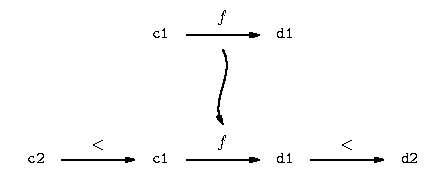
\includegraphics[scale=1.5]{subtyping-proc-type.pdf}\end{SCentered}

\caption{过程类型的子类型判定\label{t:x28elem_x22figx2d9x2e15x22x29}}\end{EoplFigure}

要理解最后一条规则,令 \texMathInline{t_1} 为 \Scribtexttt{(c1 {-}{\Stttextmore} d1)},\texMathInline{t_2} 为 \Scribtexttt{(c2 {-}{\Stttextmore} d2)},
且 \Scribtexttt{c2 {\Stttextless} c1},\Scribtexttt{d1 {\Stttextless} d2}。令 \Scribtexttt{f} 为一过程,类型为 \texMathInline{t_1}。我们说 \Scribtexttt{f}
类型也为 \texMathInline{t_2}。为什么?假设我们给 \Scribtexttt{f} 传递了类型为 \Scribtexttt{c2} 的参数。由于
\Scribtexttt{c2 {\Stttextless} c1},参数类型也是 \Scribtexttt{c1},所以 \Scribtexttt{f} 可以接受这个参数。然后,\Scribtexttt{f}返
回值类型为 \Scribtexttt{d1}。但由于 \Scribtexttt{d1 {\Stttextless} d2},这个结果类型也是 \Scribtexttt{d2}。所以,如果给
\Scribtexttt{f} 一个类型为 \Scribtexttt{c2} 的参数,其返回值类型为 \Scribtexttt{d2}。因此,\Scribtexttt{f} 类型为
\Scribtexttt{(c2 {-}{\Stttextmore} d2)}。我们说结果类型的子类型判定是\emph{协变的} (\emph{covariant}),参数类
型的子类型判定是\emph{逆变的} (\emph{contravariant})。见。这与
\SecRefLocal{t:x28part_x22s8x2e3x2e2x22x29}{8.3.2}{实现}中 \Scribtexttt{{\Stttextless}{\hbox{\texttt{:}}}{-}iface} 的定义类似。
\index{zzilei4xing2pan4ding4deni4bian4@子类型判定的逆变|(idxdecorator{}{}}
\index{zzilei4xing2pan4ding4dexie2bian4@子类型判定的协变|(idxdecorator{}{}}

这部分代码如 所示。代码使用\Scribtexttt{every2{\hbox{\texttt{?}}}},
它扩展ex1.24 中的过程 \Scribtexttt{every{\hbox{\texttt{?}}}},取一个双参数谓词和两个列表,当
列表长度相同且对应元素满足谓词时,返回 \Scribtexttt{\#t},否则返回 \Scribtexttt{\#f}。
\index{zzilei4xing2pan4ding4deni4bian4@子类型判定的逆变|)idxdecorator{}{}}
\index{zzilei4xing2pan4ding4dexie2bian4@子类型判定的协变|)idxdecorator{}{}}
\index{mzian4xiang4dui4xiang4dexiao1xi1chuan2di4fang1fa3diao4yong4@面向对象的消息传递(方法调用)|)idxdecorator{}{}}

\begin{EoplFigure}\begin{SCodeFlow}\begin{RktBlk}\begin{SingleColumn}\textbf{\Scribtexttt{check{-}is{-}subtype{\hbox{\texttt{!}}}}} : \texMathInline{\mathit{Type} \times \mathit{Type} \times \mathit{Exp} \to \mathit{Unspecified}}

\RktPn{(}\RktSym{define}\mbox{\hphantom{\Scribtexttt{x}}}\RktSym{check{-}is{-}subtype{\hbox{\texttt{!}}}}

\mbox{\hphantom{\Scribtexttt{xx}}}\RktPn{(}\RktSym{lambda}\mbox{\hphantom{\Scribtexttt{x}}}\RktPn{(}\RktSym{ty1}\mbox{\hphantom{\Scribtexttt{x}}}\RktSym{ty2}\mbox{\hphantom{\Scribtexttt{x}}}\RktSym{exp}\RktPn{)}

\mbox{\hphantom{\Scribtexttt{xxxx}}}\RktPn{(}\RktSym{if}\mbox{\hphantom{\Scribtexttt{x}}}\RktPn{(}\RktSym{is{-}subtype{\hbox{\texttt{?}}}}\mbox{\hphantom{\Scribtexttt{x}}}\RktSym{ty1}\mbox{\hphantom{\Scribtexttt{x}}}\RktSym{ty2}\RktPn{)}

\mbox{\hphantom{\Scribtexttt{xxxxxx}}}\RktVal{\#t}

\mbox{\hphantom{\Scribtexttt{xxxxxx}}}\RktPn{(}\RktSym{report{-}subtype{-}failure}

\mbox{\hphantom{\Scribtexttt{xxxxxxxx}}}\RktPn{(}\RktSym{type{-}to{-}external{-}form}\mbox{\hphantom{\Scribtexttt{x}}}\RktSym{ty1}\RktPn{)}

\mbox{\hphantom{\Scribtexttt{xxxxxxxx}}}\RktPn{(}\RktSym{type{-}to{-}external{-}form}\mbox{\hphantom{\Scribtexttt{x}}}\RktSym{ty2}\RktPn{)}

\mbox{\hphantom{\Scribtexttt{xxxxxxxx}}}\RktSym{exp}\RktPn{)}\RktPn{)}\RktPn{)}\RktPn{)}

\mbox{\hphantom{\Scribtexttt{x}}}

\textbf{\Scribtexttt{is{-}subtype{\hbox{\texttt{?}}}}} : \texMathInline{\mathit{Type} \times \mathit{Type} \to \mathit{Bool}}

\RktPn{(}\RktSym{define}\mbox{\hphantom{\Scribtexttt{x}}}\RktSym{is{-}subtype{\hbox{\texttt{?}}}}

\mbox{\hphantom{\Scribtexttt{xx}}}\RktPn{(}\RktSym{lambda}\mbox{\hphantom{\Scribtexttt{x}}}\RktPn{(}\RktSym{ty1}\mbox{\hphantom{\Scribtexttt{x}}}\RktSym{ty2}\RktPn{)}

\mbox{\hphantom{\Scribtexttt{xxxx}}}\RktPn{(}\RktSym{cases}\mbox{\hphantom{\Scribtexttt{x}}}\RktSym{type}\mbox{\hphantom{\Scribtexttt{x}}}\RktSym{ty1}

\mbox{\hphantom{\Scribtexttt{xxxxxx}}}\RktPn{(}\RktSym{class{-}type}\mbox{\hphantom{\Scribtexttt{x}}}\RktPn{(}\RktSym{name1}\RktPn{)}

\mbox{\hphantom{\Scribtexttt{xxxxxxxx}}}\RktPn{(}\RktSym{cases}\mbox{\hphantom{\Scribtexttt{x}}}\RktSym{type}\mbox{\hphantom{\Scribtexttt{x}}}\RktSym{ty2}

\mbox{\hphantom{\Scribtexttt{xxxxxxxxxx}}}\RktPn{(}\RktSym{class{-}type}\mbox{\hphantom{\Scribtexttt{x}}}\RktPn{(}\RktSym{name2}\RktPn{)}

\mbox{\hphantom{\Scribtexttt{xxxxxxxxxxxx}}}\RktPn{(}\RktSym{statically{-}is{-}subclass{\hbox{\texttt{?}}}}\mbox{\hphantom{\Scribtexttt{x}}}\RktSym{name1}\mbox{\hphantom{\Scribtexttt{x}}}\RktSym{name2}\RktPn{)}\RktPn{)}

\mbox{\hphantom{\Scribtexttt{xxxxxxxxxx}}}\RktPn{(}\RktSym{else}\mbox{\hphantom{\Scribtexttt{x}}}\RktVal{\#f}\RktPn{)}\RktPn{)}\RktPn{)}

\mbox{\hphantom{\Scribtexttt{xxxxxx}}}\RktPn{(}\RktSym{proc{-}type}\mbox{\hphantom{\Scribtexttt{x}}}\RktPn{(}\RktSym{args1}\mbox{\hphantom{\Scribtexttt{x}}}\RktSym{res1}\RktPn{)}

\mbox{\hphantom{\Scribtexttt{xxxxxxxx}}}\RktPn{(}\RktSym{cases}\mbox{\hphantom{\Scribtexttt{x}}}\RktSym{type}\mbox{\hphantom{\Scribtexttt{x}}}\RktSym{ty2}

\mbox{\hphantom{\Scribtexttt{xxxxxxxxxx}}}\RktPn{(}\RktSym{proc{-}type}\mbox{\hphantom{\Scribtexttt{x}}}\RktPn{(}\RktSym{args2}\mbox{\hphantom{\Scribtexttt{x}}}\RktSym{res2}\RktPn{)}

\mbox{\hphantom{\Scribtexttt{xxxxxxxxxxxx}}}\RktPn{(}\RktSym{and}

\mbox{\hphantom{\Scribtexttt{xxxxxxxxxxxxxx}}}\RktPn{(}\RktSym{every2{\hbox{\texttt{?}}}}\mbox{\hphantom{\Scribtexttt{x}}}\RktSym{is{-}subtype{\hbox{\texttt{?}}}}\mbox{\hphantom{\Scribtexttt{x}}}\RktSym{args2}\mbox{\hphantom{\Scribtexttt{x}}}\RktSym{args1}\RktPn{)}

\mbox{\hphantom{\Scribtexttt{xxxxxxxxxxxxxx}}}\RktPn{(}\RktSym{is{-}subtype{\hbox{\texttt{?}}}}\mbox{\hphantom{\Scribtexttt{x}}}\RktSym{res1}\mbox{\hphantom{\Scribtexttt{x}}}\RktSym{res2}\RktPn{)}\RktPn{)}\RktPn{)}

\mbox{\hphantom{\Scribtexttt{xxxxxxxxxx}}}\RktPn{(}\RktSym{else}\mbox{\hphantom{\Scribtexttt{x}}}\RktVal{\#f}\RktPn{)}\RktPn{)}\RktPn{)}

\mbox{\hphantom{\Scribtexttt{xxxxxx}}}\RktPn{(}\RktSym{else}\mbox{\hphantom{\Scribtexttt{x}}}\RktPn{(}\RktSym{equal{\hbox{\texttt{?}}}}\mbox{\hphantom{\Scribtexttt{x}}}\RktSym{ty1}\mbox{\hphantom{\Scribtexttt{x}}}\RktSym{ty2}\RktPn{)}\RktPn{)}\RktPn{)}\RktPn{)}\RktPn{)}

\mbox{\hphantom{\Scribtexttt{x}}}

\textbf{\Scribtexttt{statically{-}is{-}subclass{\hbox{\texttt{?}}}}} : \texMathInline{\mathit{ClassName} \times \mathit{ClassName} \to \mathit{Bool}}

\RktPn{(}\RktSym{define}\mbox{\hphantom{\Scribtexttt{x}}}\RktSym{statically{-}is{-}subclass{\hbox{\texttt{?}}}}

\mbox{\hphantom{\Scribtexttt{xx}}}\RktPn{(}\RktSym{lambda}\mbox{\hphantom{\Scribtexttt{x}}}\RktPn{(}\RktSym{name1}\mbox{\hphantom{\Scribtexttt{x}}}\RktSym{name2}\RktPn{)}

\mbox{\hphantom{\Scribtexttt{xxxx}}}\RktPn{(}\RktSym{or}

\mbox{\hphantom{\Scribtexttt{xxxxxx}}}\RktPn{(}\RktSym{eqv{\hbox{\texttt{?}}}}\mbox{\hphantom{\Scribtexttt{x}}}\RktSym{name1}\mbox{\hphantom{\Scribtexttt{x}}}\RktSym{name2}\RktPn{)}

\mbox{\hphantom{\Scribtexttt{xxxxxx}}}\RktPn{(}\RktSym{let}\mbox{\hphantom{\Scribtexttt{x}}}\RktPn{(}\RktPn{(}\RktSym{super{-}name}

\mbox{\hphantom{\Scribtexttt{xxxxxxxxxxxxxx}}}\RktPn{(}\RktSym{static{-}class{-}{\Stttextmore}super{-}name}

\mbox{\hphantom{\Scribtexttt{xxxxxxxxxxxxxxxx}}}\RktPn{(}\RktSym{lookup{-}static{-}class}\mbox{\hphantom{\Scribtexttt{x}}}\RktSym{name1}\RktPn{)}\RktPn{)}\RktPn{)}\RktPn{)}

\mbox{\hphantom{\Scribtexttt{xxxxxxxx}}}\RktPn{(}\RktSym{if}\mbox{\hphantom{\Scribtexttt{x}}}\RktSym{super{-}name}

\mbox{\hphantom{\Scribtexttt{xxxxxxxxxx}}}\RktPn{(}\RktSym{statically{-}is{-}subclass{\hbox{\texttt{?}}}}\mbox{\hphantom{\Scribtexttt{x}}}\RktSym{super{-}name}\mbox{\hphantom{\Scribtexttt{x}}}\RktSym{name2}\RktPn{)}

\mbox{\hphantom{\Scribtexttt{xxxxxxxxxx}}}\RktVal{\#f}\RktPn{)}\RktPn{)}

\mbox{\hphantom{\Scribtexttt{xxxxxx}}}\RktPn{(}\RktSym{let}\mbox{\hphantom{\Scribtexttt{x}}}\RktPn{(}\RktPn{(}\RktSym{interface{-}names}

\mbox{\hphantom{\Scribtexttt{xxxxxxxxxxxxxx}}}\RktPn{(}\RktSym{static{-}class{-}{\Stttextmore}interface{-}names}

\mbox{\hphantom{\Scribtexttt{xxxxxxxxxxxxxxxx}}}\RktPn{(}\RktSym{lookup{-}static{-}class}\mbox{\hphantom{\Scribtexttt{x}}}\RktSym{name1}\RktPn{)}\RktPn{)}\RktPn{)}\RktPn{)}

\mbox{\hphantom{\Scribtexttt{xxxxxxxx}}}\RktPn{(}\RktSym{memv}\mbox{\hphantom{\Scribtexttt{x}}}\RktSym{name2}\mbox{\hphantom{\Scribtexttt{x}}}\RktSym{interface{-}names}\RktPn{)}\RktPn{)}\RktPn{)}\RktPn{)}\RktPn{)}\end{SingleColumn}\end{RktBlk}\end{SCodeFlow}

\caption{TYPED{-}OO 的子类型判定
\index{zzilei4xing2pan4ding4deni4bian4@子类型判定的逆变|idxdecorator{}{}}
\index{zzilei4xing2pan4ding4dexie2bian4@子类型判定的协变|idxdecorator{}{}}\label{t:x28elem_x22figx2d9x2e16x22x29}}\end{EoplFigure}

现在可以逐一考虑三种调用()。对方法调用,我们首先像通常那
样,找出目标对象和操作数的类型。我们用类似 \Scribtexttt{find{-}method} 的
\Scribtexttt{find{-}method{-}type} 找出方法的类型。如果目标类型不是类或接口,那么
\Scribtexttt{type{-}{\Stttextmore}class{-}name} 报错。如果没有对应方法,那么 \Scribtexttt{find{-}method{-}type} 报错。
然后,我们调用 \Scribtexttt{type{-}of{-}call} 验证操作数的类型与方法的期望是否相符,并返回结
果的类型。

\begin{EoplFigure}\begin{SCodeFlow}\begin{RktBlk}\begin{SingleColumn}\mbox{\hphantom{\Scribtexttt{xxxx}}}\RktPn{(}\RktSym{method{-}call{-}exp}\RktMeta{}\mbox{\hphantom{\Scribtexttt{x}}}\RktMeta{}\RktPn{(}\RktSym{obj{-}exp}\RktMeta{}\mbox{\hphantom{\Scribtexttt{x}}}\RktMeta{}\RktSym{method{-}name}\RktMeta{}\mbox{\hphantom{\Scribtexttt{x}}}\RktMeta{}\RktSym{rands}\RktPn{)}\RktMeta{}

\mbox{\hphantom{\Scribtexttt{xxxx}}}\RktMeta{}\mbox{\hphantom{\Scribtexttt{xx}}}\RktMeta{}\RktPn{(}\RktSym{let}\RktMeta{}\mbox{\hphantom{\Scribtexttt{x}}}\RktMeta{}\RktPn{(}\RktPn{(}\RktSym{arg{-}types}\RktMeta{}\mbox{\hphantom{\Scribtexttt{x}}}\RktMeta{}\RktPn{(}\RktSym{types{-}of{-}exps}\RktMeta{}\mbox{\hphantom{\Scribtexttt{x}}}\RktMeta{}\RktSym{rands}\RktMeta{}\mbox{\hphantom{\Scribtexttt{x}}}\RktMeta{}\RktSym{tenv}\RktPn{)}\RktPn{)}\RktMeta{}

\mbox{\hphantom{\Scribtexttt{xxxx}}}\RktMeta{}\mbox{\hphantom{\Scribtexttt{xxxxxxxxx}}}\RktMeta{}\RktPn{(}\RktSym{obj{-}type}\RktMeta{}\mbox{\hphantom{\Scribtexttt{x}}}\RktMeta{}\RktPn{(}\RktSym{type{-}of}\RktMeta{}\mbox{\hphantom{\Scribtexttt{x}}}\RktMeta{}\RktSym{obj{-}exp}\RktMeta{}\mbox{\hphantom{\Scribtexttt{x}}}\RktMeta{}\RktSym{tenv}\RktPn{)}\RktPn{)}\RktPn{)}\RktMeta{}

\mbox{\hphantom{\Scribtexttt{xxxx}}}\RktMeta{}\mbox{\hphantom{\Scribtexttt{xxxx}}}\RktMeta{}\RktPn{(}\RktSym{type{-}of{-}call}\RktMeta{}

\mbox{\hphantom{\Scribtexttt{xxxx}}}\RktMeta{}\mbox{\hphantom{\Scribtexttt{xxxxxx}}}\RktMeta{}\RktPn{(}\RktSym{find{-}method{-}type}\RktMeta{}

\mbox{\hphantom{\Scribtexttt{xxxx}}}\RktMeta{}\mbox{\hphantom{\Scribtexttt{xxxxxxxx}}}\RktMeta{}\RktPn{(}\RktSym{type{-}{\Stttextmore}class{-}name}\RktMeta{}\mbox{\hphantom{\Scribtexttt{x}}}\RktMeta{}\RktSym{obj{-}type}\RktPn{)}\RktMeta{}

\mbox{\hphantom{\Scribtexttt{xxxx}}}\RktMeta{}\mbox{\hphantom{\Scribtexttt{xxxxxxxx}}}\RktMeta{}\RktSym{method{-}name}\RktPn{)}\RktMeta{}

\mbox{\hphantom{\Scribtexttt{xxxx}}}\RktMeta{}\mbox{\hphantom{\Scribtexttt{xxxxxx}}}\RktMeta{}\RktSym{arg{-}types}\RktMeta{}

\mbox{\hphantom{\Scribtexttt{xxxx}}}\RktMeta{}\mbox{\hphantom{\Scribtexttt{xxxxxx}}}\RktMeta{}\RktSym{rands}\RktMeta{}

\mbox{\hphantom{\Scribtexttt{xxxx}}}\RktMeta{}\mbox{\hphantom{\Scribtexttt{xxxxxx}}}\RktMeta{}\RktSym{exp}\RktPn{)}\RktPn{)}\RktPn{)}\RktMeta{}

\mbox{\hphantom{\Scribtexttt{xxxx}}}\RktMeta{~}

\mbox{\hphantom{\Scribtexttt{xxxx}}}\RktMeta{}\RktPn{(}\RktSym{super{-}call{-}exp}\RktMeta{}\mbox{\hphantom{\Scribtexttt{x}}}\RktMeta{}\RktPn{(}\RktSym{method{-}name}\RktMeta{}\mbox{\hphantom{\Scribtexttt{x}}}\RktMeta{}\RktSym{rands}\RktPn{)}\RktMeta{}

\mbox{\hphantom{\Scribtexttt{xxxx}}}\RktMeta{}\mbox{\hphantom{\Scribtexttt{xx}}}\RktMeta{}\RktPn{(}\RktSym{let}\RktMeta{}\mbox{\hphantom{\Scribtexttt{x}}}\RktMeta{}\RktPn{(}\RktPn{(}\RktSym{arg{-}types}\RktMeta{}\mbox{\hphantom{\Scribtexttt{x}}}\RktMeta{}\RktPn{(}\RktSym{types{-}of{-}exps}\RktMeta{}\mbox{\hphantom{\Scribtexttt{x}}}\RktMeta{}\RktSym{rands}\RktMeta{}\mbox{\hphantom{\Scribtexttt{x}}}\RktMeta{}\RktSym{tenv}\RktPn{)}\RktPn{)}\RktMeta{}

\mbox{\hphantom{\Scribtexttt{xxxx}}}\RktMeta{}\mbox{\hphantom{\Scribtexttt{xxxxxxxxx}}}\RktMeta{}\RktPn{(}\RktSym{obj{-}type}\RktMeta{}\mbox{\hphantom{\Scribtexttt{x}}}\RktMeta{}\RktPn{(}\RktSym{apply{-}tenv}\RktMeta{}\mbox{\hphantom{\Scribtexttt{x}}}\RktMeta{}\RktSym{tenv}\RktMeta{}\mbox{\hphantom{\Scribtexttt{x}}}\RktMeta{}\RktSym{{\textquotesingle}}\RktSym{\%self}\RktPn{)}\RktPn{)}\RktPn{)}\RktMeta{}

\mbox{\hphantom{\Scribtexttt{xxxx}}}\RktMeta{}\mbox{\hphantom{\Scribtexttt{xxxx}}}\RktMeta{}\RktPn{(}\RktSym{type{-}of{-}call}\RktMeta{}

\mbox{\hphantom{\Scribtexttt{xxxx}}}\RktMeta{}\mbox{\hphantom{\Scribtexttt{xxxxxx}}}\RktMeta{}\RktPn{(}\RktSym{find{-}method{-}type}\RktMeta{}

\mbox{\hphantom{\Scribtexttt{xxxx}}}\RktMeta{}\mbox{\hphantom{\Scribtexttt{xxxxxxxx}}}\RktMeta{}\RktPn{(}\RktSym{apply{-}tenv}\RktMeta{}\mbox{\hphantom{\Scribtexttt{x}}}\RktMeta{}\RktSym{tenv}\RktMeta{}\mbox{\hphantom{\Scribtexttt{x}}}\RktMeta{}\RktSym{{\textquotesingle}}\RktSym{\%super}\RktPn{)}\RktMeta{}

\mbox{\hphantom{\Scribtexttt{xxxx}}}\RktMeta{}\mbox{\hphantom{\Scribtexttt{xxxxxxxx}}}\RktMeta{}\RktSym{method{-}name}\RktPn{)}\RktMeta{}

\mbox{\hphantom{\Scribtexttt{xxxx}}}\RktMeta{}\mbox{\hphantom{\Scribtexttt{xxxxxx}}}\RktMeta{}\RktSym{arg{-}types}\RktMeta{}

\mbox{\hphantom{\Scribtexttt{xxxx}}}\RktMeta{}\mbox{\hphantom{\Scribtexttt{xxxxxx}}}\RktMeta{}\RktSym{rands}\RktMeta{}

\mbox{\hphantom{\Scribtexttt{xxxx}}}\RktMeta{}\mbox{\hphantom{\Scribtexttt{xxxxxx}}}\RktMeta{}\RktSym{exp}\RktPn{)}\RktPn{)}\RktPn{)}\RktMeta{}

\mbox{\hphantom{\Scribtexttt{xxxx}}}\RktMeta{~}

\mbox{\hphantom{\Scribtexttt{xxxx}}}\RktMeta{}\RktPn{(}\RktSym{new{-}object{-}exp}\RktMeta{}\mbox{\hphantom{\Scribtexttt{x}}}\RktMeta{}\RktPn{(}\RktSym{class{-}name}\RktMeta{}\mbox{\hphantom{\Scribtexttt{x}}}\RktMeta{}\RktSym{rands}\RktPn{)}\RktMeta{}

\mbox{\hphantom{\Scribtexttt{xxxx}}}\RktMeta{}\mbox{\hphantom{\Scribtexttt{xx}}}\RktMeta{}\RktPn{(}\RktSym{let}\RktMeta{}\mbox{\hphantom{\Scribtexttt{x}}}\RktMeta{}\RktPn{(}\RktPn{(}\RktSym{arg{-}types}\RktMeta{}\mbox{\hphantom{\Scribtexttt{x}}}\RktMeta{}\RktPn{(}\RktSym{types{-}of{-}exps}\RktMeta{}\mbox{\hphantom{\Scribtexttt{x}}}\RktMeta{}\RktSym{rands}\RktMeta{}\mbox{\hphantom{\Scribtexttt{x}}}\RktMeta{}\RktSym{tenv}\RktPn{)}\RktPn{)}\RktMeta{}

\mbox{\hphantom{\Scribtexttt{xxxx}}}\RktMeta{}\mbox{\hphantom{\Scribtexttt{xxxxxxxxx}}}\RktMeta{}\RktPn{(}\RktSym{c}\RktMeta{}\mbox{\hphantom{\Scribtexttt{x}}}\RktMeta{}\RktPn{(}\RktSym{lookup{-}static{-}class}\RktMeta{}\mbox{\hphantom{\Scribtexttt{x}}}\RktMeta{}\RktSym{class{-}name}\RktPn{)}\RktPn{)}\RktPn{)}\RktMeta{}

\mbox{\hphantom{\Scribtexttt{xxxx}}}\RktMeta{}\mbox{\hphantom{\Scribtexttt{xxxx}}}\RktMeta{}\RktPn{(}\RktSym{cases}\RktMeta{}\mbox{\hphantom{\Scribtexttt{x}}}\RktMeta{}\RktSym{static{-}class}\RktMeta{}\mbox{\hphantom{\Scribtexttt{x}}}\RktMeta{}\RktSym{c}\RktMeta{}

\mbox{\hphantom{\Scribtexttt{xxxx}}}\RktMeta{}\mbox{\hphantom{\Scribtexttt{xxxxxx}}}\RktMeta{}\RktPn{(}\RktSym{an{-}interface}\RktMeta{}\mbox{\hphantom{\Scribtexttt{x}}}\RktMeta{}\RktPn{(}\RktSym{method{-}tenv}\RktPn{)}\RktMeta{}

\mbox{\hphantom{\Scribtexttt{xxxx}}}\RktMeta{}\mbox{\hphantom{\Scribtexttt{xxxxxxxx}}}\RktMeta{}\RktPn{(}\RktSym{report{-}cant{-}instantiate{-}interface}\RktMeta{}\mbox{\hphantom{\Scribtexttt{x}}}\RktMeta{}\RktSym{class{-}name}\RktPn{)}\RktPn{)}\RktMeta{}

\mbox{\hphantom{\Scribtexttt{xxxx}}}\RktMeta{}\mbox{\hphantom{\Scribtexttt{xxxxxx}}}\RktMeta{}\RktPn{(}\RktSym{a{-}static{-}class}\RktMeta{}\mbox{\hphantom{\Scribtexttt{x}}}\RktMeta{}\RktPn{(}\RktSym{super{-}name}\RktMeta{}\mbox{\hphantom{\Scribtexttt{x}}}\RktMeta{}\RktSym{i{-}names}\RktMeta{}

\mbox{\hphantom{\Scribtexttt{xxxx}}}\RktMeta{}\mbox{\hphantom{\Scribtexttt{xxxxxxxxxxxxxxxxxxxxxxxx}}}\RktMeta{}\RktSym{field{-}names}\RktMeta{}\mbox{\hphantom{\Scribtexttt{x}}}\RktMeta{}\RktSym{field{-}types}\RktMeta{}

\mbox{\hphantom{\Scribtexttt{xxxx}}}\RktMeta{}\mbox{\hphantom{\Scribtexttt{xxxxxxxxxxxxxxxxxxxxxxxx}}}\RktMeta{}\RktSym{method{-}tenv}\RktPn{)}\RktMeta{}

\mbox{\hphantom{\Scribtexttt{xxxx}}}\RktMeta{}\mbox{\hphantom{\Scribtexttt{xxxxxxxx}}}\RktMeta{}\RktPn{(}\RktSym{type{-}of{-}call}\RktMeta{}

\mbox{\hphantom{\Scribtexttt{xxxx}}}\RktMeta{}\mbox{\hphantom{\Scribtexttt{xxxxxxxxxx}}}\RktMeta{}\RktPn{(}\RktSym{find{-}method{-}type}\RktMeta{}

\mbox{\hphantom{\Scribtexttt{xxxx}}}\RktMeta{}\mbox{\hphantom{\Scribtexttt{xxxxxxxxxxxx}}}\RktMeta{}\RktSym{class{-}name}\RktMeta{}

\mbox{\hphantom{\Scribtexttt{xxxx}}}\RktMeta{}\mbox{\hphantom{\Scribtexttt{xxxxxxxxxxxx}}}\RktMeta{}\RktSym{{\textquotesingle}}\RktSym{initialize}\RktPn{)}\RktMeta{}

\mbox{\hphantom{\Scribtexttt{xxxx}}}\RktMeta{}\mbox{\hphantom{\Scribtexttt{xxxxxxxxxx}}}\RktMeta{}\RktSym{arg{-}types}\RktMeta{}

\mbox{\hphantom{\Scribtexttt{xxxx}}}\RktMeta{}\mbox{\hphantom{\Scribtexttt{xxxxxxxxxx}}}\RktMeta{}\RktSym{rands}\RktMeta{}

\mbox{\hphantom{\Scribtexttt{xxxx}}}\RktMeta{}\mbox{\hphantom{\Scribtexttt{xxxxxxxxxx}}}\RktMeta{}\RktSym{exp}\RktPn{)}\RktMeta{}

\mbox{\hphantom{\Scribtexttt{xxxx}}}\RktMeta{}\mbox{\hphantom{\Scribtexttt{xxxxxxxx}}}\RktMeta{}\RktPn{(}\RktSym{class{-}type}\RktMeta{}\mbox{\hphantom{\Scribtexttt{x}}}\RktMeta{}\RktSym{class{-}name}\RktPn{)}\RktPn{)}\RktPn{)}\RktPn{)}\RktPn{)}\RktMeta{}\end{SingleColumn}\end{RktBlk}\end{SCodeFlow}

\caption{面向对象表达式在 \Scribtexttt{type{-}of} 中的对应语句,第 2 部分\label{t:x28elem_x22figx2d9x2e17x22x29}}\end{EoplFigure}

\index{fzen1pei4@分配!dzui4xiang4@对象|idxdecorator{}{}}
对 \Scribtexttt{new} 表达式,我们首先取出类名对应的类信息。如果没有类与名字相关联,那就报
错。之后,用操作数的类型调用 \Scribtexttt{type{-}of{-}call},检查调用 \Scribtexttt{initialize} 是否安
全。如果检查通过,那么执行表达式就是安全的。由于 \Scribtexttt{new} 表达式返回指定类的新对
象,结果类型就是对应类的类型。

TYPED{-}OO 中表达式的检查讨论完了,我们接着来构建静态类环境。

\index{lzei4huan2jing4@类环境|idxdecorator{}{}}
\index{hzuan2jing4@环境!lzei4huan2jing4@类环境|idxdecorator{}{}}
要构建静态类环境,\Scribtexttt{initialize{-}static{-}class{-}env{\hbox{\texttt{!}}}} 首先将其设置为空,然后为类
\Scribtexttt{object} 添加绑定。接着,它遍历各个类和接口声明,给静态类环境添加适当的内容。

\begin{EoplCodeInset}\begin{SCodeFlow}\begin{RktBlk}\begin{SingleColumn}\textbf{\Scribtexttt{initialize{-}static{-}class{-}env{\hbox{\texttt{!}}}}} : \texMathInline{\mathit{Listof(ClassDecl)} \to \mathit{Unspecified}}

\RktPn{(}\RktSym{define}\mbox{\hphantom{\Scribtexttt{x}}}\RktSym{initialize{-}static{-}class{-}env{\hbox{\texttt{!}}}}

\mbox{\hphantom{\Scribtexttt{xx}}}\RktPn{(}\RktSym{lambda}\mbox{\hphantom{\Scribtexttt{x}}}\RktPn{(}\RktSym{c{-}decls}\RktPn{)}

\mbox{\hphantom{\Scribtexttt{xxxx}}}\RktPn{(}\RktSym{empty{-}the{-}static{-}class{-}env{\hbox{\texttt{!}}}}\RktPn{)}

\mbox{\hphantom{\Scribtexttt{xxxx}}}\RktPn{(}\RktSym{add{-}static{-}class{-}binding{\hbox{\texttt{!}}}}

\mbox{\hphantom{\Scribtexttt{xxxxxx}}}\RktVal{{\textquotesingle}}\RktVal{object}\mbox{\hphantom{\Scribtexttt{x}}}\RktPn{(}\RktSym{a{-}static{-}class}\mbox{\hphantom{\Scribtexttt{x}}}\RktVal{\#f}\mbox{\hphantom{\Scribtexttt{x}}}\RktVal{{\textquotesingle}}\RktVal{(}\RktVal{)}\mbox{\hphantom{\Scribtexttt{x}}}\RktVal{{\textquotesingle}}\RktVal{(}\RktVal{)}\mbox{\hphantom{\Scribtexttt{x}}}\RktVal{{\textquotesingle}}\RktVal{(}\RktVal{)}\mbox{\hphantom{\Scribtexttt{x}}}\RktVal{{\textquotesingle}}\RktVal{(}\RktVal{)}\RktPn{)}\RktPn{)}

\mbox{\hphantom{\Scribtexttt{xxxx}}}\RktPn{(}\RktSym{for{-}each}\mbox{\hphantom{\Scribtexttt{x}}}\RktSym{add{-}class{-}decl{-}to{-}static{-}class{-}env{\hbox{\texttt{!}}}}\mbox{\hphantom{\Scribtexttt{x}}}\RktSym{c{-}decls}\RktPn{)}\RktPn{)}\RktPn{)}\end{SingleColumn}\end{RktBlk}\end{SCodeFlow}\end{EoplCodeInset}

\begin{EoplFigure}\begin{SCodeFlow}\begin{RktBlk}\begin{SingleColumn}\textbf{\Scribtexttt{add{-}class{-}decl{-}to{-}static{-}class{-}env{\hbox{\texttt{!}}}}} : \texMathInline{\mathit{ClassDecl} \to \mathit{Unspecified}}

\RktPn{(}\RktSym{define}\mbox{\hphantom{\Scribtexttt{x}}}\RktSym{add{-}class{-}decl{-}to{-}static{-}class{-}env{\hbox{\texttt{!}}}}

\mbox{\hphantom{\Scribtexttt{xx}}}\RktPn{(}\RktSym{lambda}\mbox{\hphantom{\Scribtexttt{x}}}\RktPn{(}\RktSym{c{-}decl}\RktPn{)}

\mbox{\hphantom{\Scribtexttt{xxxx}}}\RktPn{(}\RktSym{cases}\mbox{\hphantom{\Scribtexttt{x}}}\RktSym{class{-}decl}\mbox{\hphantom{\Scribtexttt{x}}}\RktSym{c{-}decl}

\mbox{\hphantom{\Scribtexttt{xxxxxx}}}\RktPn{(}\RktSym{an{-}interface{-}decl}\mbox{\hphantom{\Scribtexttt{x}}}\RktPn{(}\RktSym{i{-}name}\mbox{\hphantom{\Scribtexttt{x}}}\RktSym{abs{-}m{-}decls}\RktPn{)}

\mbox{\hphantom{\Scribtexttt{xxxxxxxx}}}\RktPn{(}\RktSym{let}\mbox{\hphantom{\Scribtexttt{x}}}\RktPn{(}\RktPn{(}\RktSym{m{-}tenv}

\mbox{\hphantom{\Scribtexttt{xxxxxxxxxxxxxxxx}}}\RktPn{(}\RktSym{abs{-}method{-}decls{-}{\Stttextmore}method{-}tenv}\mbox{\hphantom{\Scribtexttt{x}}}\RktSym{abs{-}m{-}decls}\RktPn{)}\RktPn{)}\RktPn{)}

\mbox{\hphantom{\Scribtexttt{xxxxxxxxxx}}}\RktPn{(}\RktSym{check{-}no{-}dups{\hbox{\texttt{!}}}}\mbox{\hphantom{\Scribtexttt{x}}}\RktPn{(}\RktSym{map}\mbox{\hphantom{\Scribtexttt{x}}}\RktSym{car}\mbox{\hphantom{\Scribtexttt{x}}}\RktSym{m{-}tenv}\RktPn{)}\mbox{\hphantom{\Scribtexttt{x}}}\RktSym{i{-}name}\RktPn{)}

\mbox{\hphantom{\Scribtexttt{xxxxxxxxxx}}}\RktPn{(}\RktSym{add{-}static{-}class{-}binding{\hbox{\texttt{!}}}}

\mbox{\hphantom{\Scribtexttt{xxxxxxxxxxxx}}}\RktSym{i{-}name}\mbox{\hphantom{\Scribtexttt{x}}}\RktPn{(}\RktSym{an{-}interface}\mbox{\hphantom{\Scribtexttt{x}}}\RktSym{m{-}tenv}\RktPn{)}\RktPn{)}\RktPn{)}\RktPn{)}

\mbox{\hphantom{\Scribtexttt{xxxxxx}}}\RktPn{(}\RktSym{a{-}class{-}decl}\mbox{\hphantom{\Scribtexttt{x}}}\RktPn{(}\RktSym{c{-}name}\mbox{\hphantom{\Scribtexttt{x}}}\RktSym{s{-}name}\mbox{\hphantom{\Scribtexttt{x}}}\RktSym{i{-}names}

\mbox{\hphantom{\Scribtexttt{xxxxxxxxxxxxxxxxxxxxxx}}}\RktSym{f{-}types}\mbox{\hphantom{\Scribtexttt{x}}}\RktSym{f{-}names}\mbox{\hphantom{\Scribtexttt{x}}}\RktSym{m{-}decls}\RktPn{)}

\mbox{\hphantom{\Scribtexttt{xxxxxxxx}}}\RktPn{(}\RktSym{let}\mbox{\hphantom{\Scribtexttt{x}}}\RktPn{(}\RktPn{(}\RktSym{i{-}names}

\mbox{\hphantom{\Scribtexttt{xxxxxxxxxxxxxxxx}}}\RktPn{(}\RktSym{append}

\mbox{\hphantom{\Scribtexttt{xxxxxxxxxxxxxxxxxx}}}\RktPn{(}\RktSym{static{-}class{-}{\Stttextmore}interface{-}names}

\mbox{\hphantom{\Scribtexttt{xxxxxxxxxxxxxxxxxxxx}}}\RktPn{(}\RktSym{lookup{-}static{-}class}\mbox{\hphantom{\Scribtexttt{x}}}\RktSym{s{-}name}\RktPn{)}\RktPn{)}

\mbox{\hphantom{\Scribtexttt{xxxxxxxxxxxxxxxxxx}}}\RktSym{i{-}names}\RktPn{)}\RktPn{)}

\mbox{\hphantom{\Scribtexttt{xxxxxxxxxxxxxxx}}}\RktPn{(}\RktSym{f{-}names}

\mbox{\hphantom{\Scribtexttt{xxxxxxxxxxxxxxxxx}}}\RktPn{(}\RktSym{append{-}field{-}names}

\mbox{\hphantom{\Scribtexttt{xxxxxxxxxxxxxxxxxxx}}}\RktPn{(}\RktSym{static{-}class{-}{\Stttextmore}field{-}names}

\mbox{\hphantom{\Scribtexttt{xxxxxxxxxxxxxxxxxxxxx}}}\RktPn{(}\RktSym{lookup{-}static{-}class}\mbox{\hphantom{\Scribtexttt{x}}}\RktSym{s{-}name}\RktPn{)}\RktPn{)}

\mbox{\hphantom{\Scribtexttt{xxxxxxxxxxxxxxxxxxx}}}\RktSym{f{-}names}\RktPn{)}\RktPn{)}

\mbox{\hphantom{\Scribtexttt{xxxxxxxxxxxxxxx}}}\RktPn{(}\RktSym{f{-}types}

\mbox{\hphantom{\Scribtexttt{xxxxxxxxxxxxxxxxx}}}\RktPn{(}\RktSym{append}

\mbox{\hphantom{\Scribtexttt{xxxxxxxxxxxxxxxxxxx}}}\RktPn{(}\RktSym{static{-}class{-}{\Stttextmore}field{-}types}

\mbox{\hphantom{\Scribtexttt{xxxxxxxxxxxxxxxxxxxxx}}}\RktPn{(}\RktSym{lookup{-}static{-}class}\mbox{\hphantom{\Scribtexttt{x}}}\RktSym{s{-}name}\RktPn{)}\RktPn{)}

\mbox{\hphantom{\Scribtexttt{xxxxxxxxxxxxxxxxxxx}}}\RktSym{f{-}types}\RktPn{)}\RktPn{)}

\mbox{\hphantom{\Scribtexttt{xxxxxxxxxxxxxxx}}}\RktPn{(}\RktSym{method{-}tenv}

\mbox{\hphantom{\Scribtexttt{xxxxxxxxxxxxxxxxx}}}\RktPn{(}\RktSym{let}\mbox{\hphantom{\Scribtexttt{x}}}\RktPn{(}\RktPn{(}\RktSym{local{-}method{-}tenv}

\mbox{\hphantom{\Scribtexttt{xxxxxxxxxxxxxxxxxxxxxxxxx}}}\RktPn{(}\RktSym{method{-}decls{-}{\Stttextmore}method{-}tenv}\mbox{\hphantom{\Scribtexttt{x}}}\RktSym{m{-}decls}\RktPn{)}\RktPn{)}\RktPn{)}

\mbox{\hphantom{\Scribtexttt{xxxxxxxxxxxxxxxxxxx}}}\RktPn{(}\RktSym{check{-}no{-}dups{\hbox{\texttt{!}}}}

\mbox{\hphantom{\Scribtexttt{xxxxxxxxxxxxxxxxxxxxx}}}\RktPn{(}\RktSym{map}\mbox{\hphantom{\Scribtexttt{x}}}\RktSym{car}\mbox{\hphantom{\Scribtexttt{x}}}\RktSym{local{-}method{-}tenv}\RktPn{)}\mbox{\hphantom{\Scribtexttt{x}}}\RktSym{c{-}name}\RktPn{)}

\mbox{\hphantom{\Scribtexttt{xxxxxxxxxxxxxxxxxxx}}}\RktPn{(}\RktSym{merge{-}method{-}tenvs}

\mbox{\hphantom{\Scribtexttt{xxxxxxxxxxxxxxxxxxxxx}}}\RktPn{(}\RktSym{static{-}class{-}{\Stttextmore}method{-}tenv}

\mbox{\hphantom{\Scribtexttt{xxxxxxxxxxxxxxxxxxxxxxx}}}\RktPn{(}\RktSym{lookup{-}static{-}class}\mbox{\hphantom{\Scribtexttt{x}}}\RktSym{s{-}name}\RktPn{)}\RktPn{)}

\mbox{\hphantom{\Scribtexttt{xxxxxxxxxxxxxxxxxxxxx}}}\RktSym{local{-}method{-}tenv}\RktPn{)}\RktPn{)}\RktPn{)}\RktPn{)}

\mbox{\hphantom{\Scribtexttt{xxxxxxxxxx}}}\RktPn{(}\RktSym{check{-}no{-}dups{\hbox{\texttt{!}}}}\mbox{\hphantom{\Scribtexttt{x}}}\RktSym{i{-}names}\mbox{\hphantom{\Scribtexttt{x}}}\RktSym{c{-}name}\RktPn{)}

\mbox{\hphantom{\Scribtexttt{xxxxxxxxxx}}}\RktPn{(}\RktSym{check{-}no{-}dups{\hbox{\texttt{!}}}}\mbox{\hphantom{\Scribtexttt{x}}}\RktSym{f{-}names}\mbox{\hphantom{\Scribtexttt{x}}}\RktSym{c{-}name}\RktPn{)}

\mbox{\hphantom{\Scribtexttt{xxxxxxxxxx}}}\RktPn{(}\RktSym{check{-}for{-}initialize{\hbox{\texttt{!}}}}\mbox{\hphantom{\Scribtexttt{x}}}\RktSym{method{-}tenv}\mbox{\hphantom{\Scribtexttt{x}}}\RktSym{c{-}name}\RktPn{)}

\mbox{\hphantom{\Scribtexttt{xxxxxxxxxx}}}\RktPn{(}\RktSym{add{-}static{-}class{-}binding{\hbox{\texttt{!}}}}\mbox{\hphantom{\Scribtexttt{x}}}\RktSym{c{-}name}

\mbox{\hphantom{\Scribtexttt{xxxxxxxxxxxx}}}\RktPn{(}\RktSym{a{-}static{-}class}

\mbox{\hphantom{\Scribtexttt{xxxxxxxxxxxxxx}}}\RktSym{s{-}name}\mbox{\hphantom{\Scribtexttt{x}}}\RktSym{i{-}names}\mbox{\hphantom{\Scribtexttt{x}}}\RktSym{f{-}names}\mbox{\hphantom{\Scribtexttt{x}}}\RktSym{f{-}types}\mbox{\hphantom{\Scribtexttt{x}}}\RktSym{method{-}tenv}\RktPn{)}\RktPn{)}\RktPn{)}\RktPn{)}\RktPn{)}\RktPn{)}\RktPn{)}\end{SingleColumn}\end{RktBlk}\end{SCodeFlow}

\caption{\Scribtexttt{add{-}class{-}decl{-}to{-}static{-}class{-}env{\hbox{\texttt{!}}}}\label{t:x28elem_x22figx2d9x2e18x22x29}}\end{EoplFigure}

过程 \Scribtexttt{add{-}class{-}decl{-}to{-}static{-}class{-}env{\hbox{\texttt{!}}}}()承担创建静
态类的艰巨工作。对每个类,我们必须收集其接口、字段和方法:

\begin{itemize}\atItemizeStart

\item 类实现父类实现的任何接口,以及自身声称实现的接口。

\item 类具有父类的所有字段,以及自身的字段,但是父类字段被当前声明的字段遮蔽。
所以,\Scribtexttt{field{-}names} 由 \Scribtexttt{append{-}field{-}names} 计算而得,就像
\Scribtexttt{initialize{-}class{-}env{\hbox{\texttt{!}}}} 那样(initialize{-}class{-}env)。

\item 类字段的类型包括父类字段的类型,以及自身声明字段的类型。

\item 类的方法包括父类的和自身的,方法带有声明类型。我们用 \Scribtexttt{proc{-}type}
\index{czhong2zai3fang1fa3@重载方法|idxdecorator{}{}} 记录方法的类型。我们把当前声明的方法放在前面,
因为它们覆盖父类的方法。

\item 我们确保当前类中声明的方法名、接口名和字段名不重复。我们还确保类中一定有
\Scribtexttt{initialize} 方法。\end{itemize}

\index{jzie1kou3@接口!lzei4@类|idxdecorator{}{}}
对接口声明,我们只需处理方法名和类型。

\index{lzei4huan2jing4@类环境|(idxdecorator{}{}}
\index{lzei4@类!szheng1ming2@声明|idxdecorator{}{}}
\index{szheng1ming2@声明!lzei4@类|idxdecorator{}{}}
\index{hzuan2jing4@环境!lzei4huan2jing4@类环境|(idxdecorator{}{}}
一旦建立了静态类环境,我们可以检查每个类声明。这由
\Scribtexttt{check{-}class{-}decl{\hbox{\texttt{!}}}}()完成。对接口,什么都不必检查。对
类声明,我们传递从静态类环境收集到的信息,检查每个方法。最后,我们检查类是否实现
了它声称实现的每个接口。

\begin{EoplFigure}[!t]

\begin{SCodeFlow}\begin{RktBlk}\begin{SingleColumn}\textbf{\Scribtexttt{check{-}class{-}decl{\hbox{\texttt{!}}}}} : \texMathInline{\mathit{ClassDecl} \to \mathit{Unspecified}}

\RktPn{(}\RktSym{define}\mbox{\hphantom{\Scribtexttt{x}}}\RktSym{check{-}class{-}decl{\hbox{\texttt{!}}}}

\mbox{\hphantom{\Scribtexttt{xx}}}\RktPn{(}\RktSym{lambda}\mbox{\hphantom{\Scribtexttt{x}}}\RktPn{(}\RktSym{c{-}decl}\RktPn{)}

\mbox{\hphantom{\Scribtexttt{xxxx}}}\RktPn{(}\RktSym{cases}\mbox{\hphantom{\Scribtexttt{x}}}\RktSym{class{-}decl}\mbox{\hphantom{\Scribtexttt{x}}}\RktSym{c{-}decl}

\mbox{\hphantom{\Scribtexttt{xxxxxx}}}\RktPn{(}\RktSym{an{-}interface{-}decl}\mbox{\hphantom{\Scribtexttt{x}}}\RktPn{(}\RktSym{i{-}name}\mbox{\hphantom{\Scribtexttt{x}}}\RktSym{abs{-}method{-}decls}\RktPn{)}

\mbox{\hphantom{\Scribtexttt{xxxxxxxx}}}\RktVal{\#t}\RktPn{)}

\mbox{\hphantom{\Scribtexttt{xxxxxx}}}\RktPn{(}\RktSym{a{-}class{-}decl}\mbox{\hphantom{\Scribtexttt{x}}}\RktPn{(}\RktSym{class{-}name}\mbox{\hphantom{\Scribtexttt{x}}}\RktSym{super{-}name}\mbox{\hphantom{\Scribtexttt{x}}}\RktSym{i{-}names}

\mbox{\hphantom{\Scribtexttt{xxxxxxxxxxxxxxxxxxxxxx}}}\RktSym{field{-}types}\mbox{\hphantom{\Scribtexttt{x}}}\RktSym{field{-}names}\mbox{\hphantom{\Scribtexttt{x}}}\RktSym{method{-}decls}\RktPn{)}

\mbox{\hphantom{\Scribtexttt{xxxxxxxx}}}\RktPn{(}\RktSym{let}\mbox{\hphantom{\Scribtexttt{x}}}\RktPn{(}\RktPn{(}\RktSym{sc}\mbox{\hphantom{\Scribtexttt{x}}}\RktPn{(}\RktSym{lookup{-}static{-}class}\mbox{\hphantom{\Scribtexttt{x}}}\RktSym{class{-}name}\RktPn{)}\RktPn{)}\RktPn{)}

\mbox{\hphantom{\Scribtexttt{xxxxxxxxxx}}}\RktPn{(}\RktSym{for{-}each}

\mbox{\hphantom{\Scribtexttt{xxxxxxxxxxxx}}}\RktPn{(}\RktSym{lambda}\mbox{\hphantom{\Scribtexttt{x}}}\RktPn{(}\RktSym{method{-}decl}\RktPn{)}

\mbox{\hphantom{\Scribtexttt{xxxxxxxxxxxxxx}}}\RktPn{(}\RktSym{check{-}method{-}decl{\hbox{\texttt{!}}}}\mbox{\hphantom{\Scribtexttt{x}}}\RktSym{method{-}decl}

\mbox{\hphantom{\Scribtexttt{xxxxxxxxxxxxxxxx}}}\RktSym{class{-}name}\mbox{\hphantom{\Scribtexttt{x}}}\RktSym{super{-}name}

\mbox{\hphantom{\Scribtexttt{xxxxxxxxxxxxxxxx}}}\RktPn{(}\RktSym{static{-}class{-}{\Stttextmore}field{-}names}\mbox{\hphantom{\Scribtexttt{x}}}\RktSym{sc}\RktPn{)}

\mbox{\hphantom{\Scribtexttt{xxxxxxxxxxxxxxxx}}}\RktPn{(}\RktSym{static{-}class{-}{\Stttextmore}field{-}types}\mbox{\hphantom{\Scribtexttt{x}}}\RktSym{sc}\RktPn{)}\RktPn{)}\RktPn{)}

\mbox{\hphantom{\Scribtexttt{xxxxxxxxxxxx}}}\RktSym{method{-}decls}\RktPn{)}\RktPn{)}

\mbox{\hphantom{\Scribtexttt{xxxxxxxx}}}\RktPn{(}\RktSym{for{-}each}

\mbox{\hphantom{\Scribtexttt{xxxxxxxxxx}}}\RktPn{(}\RktSym{lambda}\mbox{\hphantom{\Scribtexttt{x}}}\RktPn{(}\RktSym{i{-}name}\RktPn{)}

\mbox{\hphantom{\Scribtexttt{xxxxxxxxxxxx}}}\RktPn{(}\RktSym{check{-}if{-}implements{\hbox{\texttt{!}}}}\mbox{\hphantom{\Scribtexttt{x}}}\RktSym{class{-}name}\mbox{\hphantom{\Scribtexttt{x}}}\RktSym{i{-}name}\RktPn{)}\RktPn{)}

\mbox{\hphantom{\Scribtexttt{xxxxxxxxxx}}}\RktSym{i{-}names}\RktPn{)}\RktPn{)}\RktPn{)}\RktPn{)}\RktPn{)}\end{SingleColumn}\end{RktBlk}\end{SCodeFlow}

\caption{\Scribtexttt{check{-}class{-}decl{\hbox{\texttt{!}}}}
\index{lzei4huan2jing4@类环境|idxdecorator{}{}}
\index{lzei4@类!szheng1ming2@声明|idxdecorator{}{}}
\index{szheng1ming2@声明!lzei4@类|idxdecorator{}{}}\label{t:x28elem_x22figx2d9x2e19x22x29}}\end{EoplFigure}

\index{szheng1ming2@声明!fzang1fa3@方法|idxdecorator{}{}}
\index{dzui4xiang4fang1fa3@对象方法!szheng1ming2@声明|idxdecorator{}{}}
要检查方法声明,我们首先检查其主体是否符合声明类型。要这样做,我们建立一个类型环
境,该环境与主体求值时的环境相符。然后我们检查主体的结果类型是否为声明中结果类型
的子类型。

\begin{EoplFigure}[!ht]

\begin{SCodeFlow}\begin{RktBlk}\begin{SingleColumn}\textbf{\Scribtexttt{check{-}method{-}decl{\hbox{\texttt{!}}}}} : \hspace*{\fill}\\ \texMathInline{\phantom{x}\mathit{MethodDecl} \times \mathit{ClassName} \times \mathit{ClassName} \times \mathit{Listof(FieldName)} \times \mathit{Listof(Type)} \\ \phantom{xxxx}\to \mathit{Unspecified}}

\RktPn{(}\RktSym{define}\mbox{\hphantom{\Scribtexttt{x}}}\RktSym{check{-}method{-}decl{\hbox{\texttt{!}}}}

\mbox{\hphantom{\Scribtexttt{xx}}}\RktPn{(}\RktSym{lambda}\mbox{\hphantom{\Scribtexttt{x}}}\RktPn{(}\RktSym{m{-}decl}\mbox{\hphantom{\Scribtexttt{x}}}\RktSym{self{-}name}\mbox{\hphantom{\Scribtexttt{x}}}\RktSym{s{-}name}\mbox{\hphantom{\Scribtexttt{x}}}\RktSym{f{-}names}\mbox{\hphantom{\Scribtexttt{x}}}\RktSym{f{-}types}\RktPn{)}

\mbox{\hphantom{\Scribtexttt{xxxx}}}\RktPn{(}\RktSym{cases}\mbox{\hphantom{\Scribtexttt{x}}}\RktSym{method{-}decl}\mbox{\hphantom{\Scribtexttt{x}}}\RktSym{m{-}decl}

\mbox{\hphantom{\Scribtexttt{xxxxxx}}}\RktPn{(}\RktSym{a{-}method{-}decl}\mbox{\hphantom{\Scribtexttt{x}}}\RktPn{(}\RktSym{res{-}type}\mbox{\hphantom{\Scribtexttt{x}}}\RktSym{m{-}name}\mbox{\hphantom{\Scribtexttt{x}}}\RktSym{vars}\mbox{\hphantom{\Scribtexttt{x}}}\RktSym{var{-}types}\mbox{\hphantom{\Scribtexttt{x}}}\RktSym{body}\RktPn{)}

\mbox{\hphantom{\Scribtexttt{xxxxxxxx}}}\RktPn{(}\RktSym{let}\mbox{\hphantom{\Scribtexttt{x}}}\RktPn{(}\RktPn{(}\RktSym{tenv}

\mbox{\hphantom{\Scribtexttt{xxxxxxxxxxxxxxxx}}}\RktPn{(}\RktSym{extend{-}tenv}

\mbox{\hphantom{\Scribtexttt{xxxxxxxxxxxxxxxxxx}}}\RktSym{vars}\mbox{\hphantom{\Scribtexttt{x}}}\RktSym{var{-}types}

\mbox{\hphantom{\Scribtexttt{xxxxxxxxxxxxxxxxxx}}}\RktPn{(}\RktSym{extend{-}tenv{-}with{-}self{-}and{-}super}

\mbox{\hphantom{\Scribtexttt{xxxxxxxxxxxxxxxxxxxx}}}\RktPn{(}\RktSym{class{-}type}\mbox{\hphantom{\Scribtexttt{x}}}\RktSym{self{-}name}\RktPn{)}

\mbox{\hphantom{\Scribtexttt{xxxxxxxxxxxxxxxxxxxx}}}\RktSym{s{-}name}

\mbox{\hphantom{\Scribtexttt{xxxxxxxxxxxxxxxxxxxx}}}\RktPn{(}\RktSym{extend{-}tenv}\mbox{\hphantom{\Scribtexttt{x}}}\RktSym{f{-}names}\mbox{\hphantom{\Scribtexttt{x}}}\RktSym{f{-}types}

\mbox{\hphantom{\Scribtexttt{xxxxxxxxxxxxxxxxxxxxxx}}}\RktPn{(}\RktSym{init{-}tenv}\RktPn{)}\RktPn{)}\RktPn{)}\RktPn{)}\RktPn{)}\RktPn{)}

\mbox{\hphantom{\Scribtexttt{xxxxxxxxxx}}}\RktPn{(}\RktSym{let}\mbox{\hphantom{\Scribtexttt{x}}}\RktPn{(}\RktPn{(}\RktSym{body{-}type}\mbox{\hphantom{\Scribtexttt{x}}}\RktPn{(}\RktSym{type{-}of}\mbox{\hphantom{\Scribtexttt{x}}}\RktSym{body}\mbox{\hphantom{\Scribtexttt{x}}}\RktSym{tenv}\RktPn{)}\RktPn{)}\RktPn{)}

\mbox{\hphantom{\Scribtexttt{xxxxxxxxxxxx}}}\RktPn{(}\RktSym{check{-}is{-}subtype{\hbox{\texttt{!}}}}\mbox{\hphantom{\Scribtexttt{x}}}\RktSym{body{-}type}\mbox{\hphantom{\Scribtexttt{x}}}\RktSym{res{-}type}\mbox{\hphantom{\Scribtexttt{x}}}\RktSym{m{-}decl}\RktPn{)}

\mbox{\hphantom{\Scribtexttt{xxxxxxxxxxxx}}}\RktPn{(}\RktSym{if}\mbox{\hphantom{\Scribtexttt{x}}}\RktPn{(}\RktSym{eqv{\hbox{\texttt{?}}}}\mbox{\hphantom{\Scribtexttt{x}}}\RktSym{m{-}name}\mbox{\hphantom{\Scribtexttt{x}}}\RktVal{{\textquotesingle}}\RktVal{initialize}\RktPn{)}\mbox{\hphantom{\Scribtexttt{x}}}\RktVal{\#t}

\mbox{\hphantom{\Scribtexttt{xxxxxxxxxxxxxx}}}\RktPn{(}\RktSym{let}\mbox{\hphantom{\Scribtexttt{x}}}\RktPn{(}\RktPn{(}\RktSym{maybe{-}super{-}type}

\mbox{\hphantom{\Scribtexttt{xxxxxxxxxxxxxxxxxxxxxx}}}\RktPn{(}\RktSym{maybe{-}find{-}method{-}type}

\mbox{\hphantom{\Scribtexttt{xxxxxxxxxxxxxxxxxxxxxxxx}}}\RktPn{(}\RktSym{static{-}class{-}{\Stttextmore}method{-}tenv}

\mbox{\hphantom{\Scribtexttt{xxxxxxxxxxxxxxxxxxxxxxxxxx}}}\RktPn{(}\RktSym{lookup{-}static{-}class}\mbox{\hphantom{\Scribtexttt{x}}}\RktSym{s{-}name}\RktPn{)}\RktPn{)}

\mbox{\hphantom{\Scribtexttt{xxxxxxxxxxxxxxxxxxxxxxxx}}}\RktSym{m{-}name}\RktPn{)}\RktPn{)}\RktPn{)}

\mbox{\hphantom{\Scribtexttt{xxxxxxxxxxxxxxxx}}}\RktPn{(}\RktSym{if}\mbox{\hphantom{\Scribtexttt{x}}}\RktSym{maybe{-}super{-}type}

\mbox{\hphantom{\Scribtexttt{xxxxxxxxxxxxxxxxxx}}}\RktPn{(}\RktSym{check{-}is{-}subtype{\hbox{\texttt{!}}}}

\mbox{\hphantom{\Scribtexttt{xxxxxxxxxxxxxxxxxxxx}}}\RktPn{(}\RktSym{proc{-}type}\mbox{\hphantom{\Scribtexttt{x}}}\RktSym{var{-}types}\mbox{\hphantom{\Scribtexttt{x}}}\RktSym{res{-}type}\RktPn{)}

\mbox{\hphantom{\Scribtexttt{xxxxxxxxxxxxxxxxxxxx}}}\RktSym{maybe{-}super{-}type}\mbox{\hphantom{\Scribtexttt{x}}}\RktSym{body}\RktPn{)}

\mbox{\hphantom{\Scribtexttt{xxxxxxxxxxxxxxxxxx}}}\RktVal{\#t}\RktPn{)}\RktPn{)}\RktPn{)}\RktPn{)}\RktPn{)}\RktPn{)}\RktPn{)}\RktPn{)}\RktPn{)}\end{SingleColumn}\end{RktBlk}\end{SCodeFlow}

\caption{\Scribtexttt{check{-}method{-}decl{\hbox{\texttt{!}}}}
\index{szheng1ming2@声明!fzang1fa3@方法|idxdecorator{}{}}
\index{dzui4xiang4fang1fa3@对象方法!szheng1ming2@声明|idxdecorator{}{}}
\index{lzei4xing2jian3cha2@类型检查!mzian4xiang4dui4xiang4@面向对象|idxdecorator{}{}}\label{t:x28elem_x22figx2d9x2e20x22x29}}\end{EoplFigure}

但还没完:如果这个方法覆盖了超类中的某个方法,我们要确保它的类型兼容超类中的方法
类型。之所以如此,是因为这个方法可能由另一方法调用,而另一方法只知道超类方法的类
型。这条规则的唯一例外是 \Scribtexttt{initialize},它只在当前类中调用,且随继承改变类型
(见)。要这样做,它调用 \Scribtexttt{maybe{-}find{-}method{-}type},后者
返回已绑定方法的类型,或者 \Scribtexttt{\#f}。见。

如,过程 \Scribtexttt{check{-}if{-}implements{\hbox{\texttt{?}}}} 取两个符号,分别为类名和
接口名。它首先检查两个符号确实为类名和接口名。然后,它遍历接口中的每个方法,检查
类是否提供了同名且类型兼容的方法。

为 中示例程序生成的静态类环境如 所示。
静态类是逆序的,这反映了生成类环境的顺序。三个类中的方法顺序相同,且类型相同,符
合期望。

这样,检查器就完成了。
\index{lzei4huan2jing4@类环境|)idxdecorator{}{}}
\index{lzei4xing2jian3cha2@类型检查!mzian4xiang4dui4xiang4@面向对象|)idxdecorator{}{}}

\begin{EoplFigure}[!t]

\begin{SCodeFlow}\begin{RktBlk}\begin{SingleColumn}\textbf{\Scribtexttt{check{-}if{-}implements{\hbox{\texttt{!}}}}} : \texMathInline{\mathit{ClassName} \times \mathit{InterfaceName} \to \mathit{Bool}}

\RktPn{(}\RktSym{define}\mbox{\hphantom{\Scribtexttt{x}}}\RktSym{check{-}if{-}implements{\hbox{\texttt{!}}}}

\mbox{\hphantom{\Scribtexttt{xx}}}\RktPn{(}\RktSym{lambda}\mbox{\hphantom{\Scribtexttt{x}}}\RktPn{(}\RktSym{c{-}name}\mbox{\hphantom{\Scribtexttt{x}}}\RktSym{i{-}name}\RktPn{)}

\mbox{\hphantom{\Scribtexttt{xxxx}}}\RktPn{(}\RktSym{cases}\mbox{\hphantom{\Scribtexttt{x}}}\RktSym{static{-}class}\mbox{\hphantom{\Scribtexttt{x}}}\RktPn{(}\RktSym{lookup{-}static{-}class}\mbox{\hphantom{\Scribtexttt{x}}}\RktSym{i{-}name}\RktPn{)}

\mbox{\hphantom{\Scribtexttt{xxxxxx}}}\RktPn{(}\RktSym{a{-}static{-}class}\mbox{\hphantom{\Scribtexttt{x}}}\RktPn{(}\RktSym{s{-}name}\mbox{\hphantom{\Scribtexttt{x}}}\RktSym{i{-}names}\mbox{\hphantom{\Scribtexttt{x}}}\RktSym{f{-}names}\mbox{\hphantom{\Scribtexttt{x}}}\RktSym{f{-}types}

\mbox{\hphantom{\Scribtexttt{xxxxxxxxxxxxxxxxxxxxxxxx}}}\RktSym{m{-}tenv}\RktPn{)}

\mbox{\hphantom{\Scribtexttt{xxxxxxxx}}}\RktPn{(}\RktSym{report{-}cant{-}implement{-}non{-}interface}

\mbox{\hphantom{\Scribtexttt{xxxxxxxxxx}}}\RktSym{c{-}name}\mbox{\hphantom{\Scribtexttt{x}}}\RktSym{i{-}name}\RktPn{)}\RktPn{)}

\mbox{\hphantom{\Scribtexttt{xxxxxx}}}\RktPn{(}\RktSym{an{-}interface}\mbox{\hphantom{\Scribtexttt{x}}}\RktPn{(}\RktSym{method{-}tenv}\RktPn{)}

\mbox{\hphantom{\Scribtexttt{xxxxxxxx}}}\RktPn{(}\RktSym{let}\mbox{\hphantom{\Scribtexttt{x}}}\RktPn{(}\RktPn{(}\RktSym{class{-}method{-}tenv}

\mbox{\hphantom{\Scribtexttt{xxxxxxxxxxxxxxxx}}}\RktPn{(}\RktSym{static{-}class{-}{\Stttextmore}method{-}tenv}

\mbox{\hphantom{\Scribtexttt{xxxxxxxxxxxxxxxxxx}}}\RktPn{(}\RktSym{lookup{-}static{-}class}\mbox{\hphantom{\Scribtexttt{x}}}\RktSym{c{-}name}\RktPn{)}\RktPn{)}\RktPn{)}\RktPn{)}

\mbox{\hphantom{\Scribtexttt{xxxxxxxxxx}}}\RktPn{(}\RktSym{for{-}each}

\mbox{\hphantom{\Scribtexttt{xxxxxxxxxxxx}}}\RktPn{(}\RktSym{lambda}\mbox{\hphantom{\Scribtexttt{x}}}\RktPn{(}\RktSym{method{-}binding}\RktPn{)}

\mbox{\hphantom{\Scribtexttt{xxxxxxxxxxxxxx}}}\RktPn{(}\RktSym{let}\mbox{\hphantom{\Scribtexttt{x}}}\RktPn{(}\RktPn{(}\RktSym{m{-}name}\mbox{\hphantom{\Scribtexttt{x}}}\RktPn{(}\RktSym{car}\mbox{\hphantom{\Scribtexttt{x}}}\RktSym{method{-}binding}\RktPn{)}\RktPn{)}

\mbox{\hphantom{\Scribtexttt{xxxxxxxxxxxxxxxxxxxxx}}}\RktPn{(}\RktSym{m{-}type}\mbox{\hphantom{\Scribtexttt{x}}}\RktPn{(}\RktSym{cadr}\mbox{\hphantom{\Scribtexttt{x}}}\RktSym{method{-}binding}\RktPn{)}\RktPn{)}\RktPn{)}

\mbox{\hphantom{\Scribtexttt{xxxxxxxxxxxxxxxx}}}\RktPn{(}\RktSym{let}\mbox{\hphantom{\Scribtexttt{x}}}\RktPn{(}\RktPn{(}\RktSym{c{-}method{-}type}

\mbox{\hphantom{\Scribtexttt{xxxxxxxxxxxxxxxxxxxxxxxx}}}\RktPn{(}\RktSym{maybe{-}find{-}method{-}type}

\mbox{\hphantom{\Scribtexttt{xxxxxxxxxxxxxxxxxxxxxxxxxx}}}\RktSym{class{-}method{-}tenv}

\mbox{\hphantom{\Scribtexttt{xxxxxxxxxxxxxxxxxxxxxxxxxx}}}\RktSym{m{-}name}\RktPn{)}\RktPn{)}\RktPn{)}

\mbox{\hphantom{\Scribtexttt{xxxxxxxxxxxxxxxxxx}}}\RktPn{(}\RktSym{if}\mbox{\hphantom{\Scribtexttt{x}}}\RktSym{c{-}method{-}type}

\mbox{\hphantom{\Scribtexttt{xxxxxxxxxxxxxxxxxxxx}}}\RktPn{(}\RktSym{check{-}is{-}subtype{\hbox{\texttt{!}}}}

\mbox{\hphantom{\Scribtexttt{xxxxxxxxxxxxxxxxxxxxxx}}}\RktSym{c{-}method{-}type}\mbox{\hphantom{\Scribtexttt{x}}}\RktSym{m{-}type}\mbox{\hphantom{\Scribtexttt{x}}}\RktSym{c{-}name}\RktPn{)}

\mbox{\hphantom{\Scribtexttt{xxxxxxxxxxxxxxxxxxxx}}}\RktPn{(}\RktSym{report{-}missing{-}method}

\mbox{\hphantom{\Scribtexttt{xxxxxxxxxxxxxxxxxxxxxx}}}\RktSym{c{-}name}\mbox{\hphantom{\Scribtexttt{x}}}\RktSym{i{-}name}\mbox{\hphantom{\Scribtexttt{x}}}\RktSym{m{-}name}\RktPn{)}\RktPn{)}\RktPn{)}\RktPn{)}\RktPn{)}

\mbox{\hphantom{\Scribtexttt{xxxxxxxxxxxx}}}\RktSym{method{-}tenv}\RktPn{)}\RktPn{)}\RktPn{)}\RktPn{)}\RktPn{)}\RktPn{)}\end{SingleColumn}\end{RktBlk}\end{SCodeFlow}

\caption{\Scribtexttt{check{-}if{-}implements{\hbox{\texttt{!}}}}
\index{jzie1kou3@接口!lzei4@类|idxdecorator{}{}}
\index{lzei4xing2jian3cha2@类型检查!mzian4xiang4dui4xiang4@面向对象|idxdecorator{}{}}\label{t:x28elem_x22figx2d9x2e21x22x29}}\end{EoplFigure}

\begin{EoplFigure}\begin{SCodeFlow}\begin{RktBlk}\begin{SingleColumn}\RktPn{(}\RktPn{(}\RktSym{leaf{-}node}

\mbox{\hphantom{\Scribtexttt{xxx}}}\RktVal{\#}\RktVal{(}\RktVal{struct{\hbox{\texttt{:}}}a{-}static{-}class}

\mbox{\hphantom{\Scribtexttt{xxxxxx}}}\RktVal{object}

\mbox{\hphantom{\Scribtexttt{xxxxxx}}}\RktVal{(}\RktVal{tree}\RktVal{)}

\mbox{\hphantom{\Scribtexttt{xxxxxx}}}\RktVal{(}\RktVal{value}\RktVal{)}

\mbox{\hphantom{\Scribtexttt{xxxxxx}}}\RktVal{(}\RktVal{\#}\RktVal{(}\RktVal{struct{\hbox{\texttt{:}}}int{-}type}\RktVal{)}\RktVal{)}

\mbox{\hphantom{\Scribtexttt{xxxxxx}}}\RktVal{(}\RktVal{(}\RktVal{initialize}\mbox{\hphantom{\Scribtexttt{x}}}\RktVal{\#}\RktVal{(}\RktVal{struct{\hbox{\texttt{:}}}proc{-}type}

\mbox{\hphantom{\Scribtexttt{xxxxxxxxxxxxxxxxxxxxxx}}}\RktVal{(}\RktVal{\#}\RktVal{(}\RktVal{struct{\hbox{\texttt{:}}}int{-}type}\RktVal{)}\RktVal{)}

\mbox{\hphantom{\Scribtexttt{xxxxxxxxxxxxxxxxxxxxxx}}}\RktVal{\#}\RktVal{(}\RktVal{struct{\hbox{\texttt{:}}}void{-}type}\RktVal{)}\RktVal{)}\RktVal{)}

\mbox{\hphantom{\Scribtexttt{xxxxxxxx}}}\RktVal{(}\RktVal{sum}\mbox{\hphantom{\Scribtexttt{x}}}\RktVal{\#}\RktVal{(}\RktVal{struct{\hbox{\texttt{:}}}proc{-}type}\mbox{\hphantom{\Scribtexttt{x}}}\RktVal{(}\RktVal{)}\mbox{\hphantom{\Scribtexttt{x}}}\RktVal{\#}\RktVal{(}\RktVal{struct{\hbox{\texttt{:}}}int{-}type}\RktVal{)}\RktVal{)}\RktVal{)}

\mbox{\hphantom{\Scribtexttt{xxxxxxxx}}}\RktVal{(}\RktVal{getvalue}\mbox{\hphantom{\Scribtexttt{x}}}\RktVal{\#}\RktVal{(}\RktVal{struct{\hbox{\texttt{:}}}proc{-}type}\mbox{\hphantom{\Scribtexttt{x}}}\RktVal{(}\RktVal{)}\mbox{\hphantom{\Scribtexttt{x}}}\RktVal{\#}\RktVal{(}\RktVal{struct{\hbox{\texttt{:}}}int{-}type}\RktVal{)}\RktVal{)}\RktVal{)}

\mbox{\hphantom{\Scribtexttt{xxxxxxxx}}}\RktVal{(}\RktVal{equal}\mbox{\hphantom{\Scribtexttt{x}}}\RktVal{\#}\RktVal{(}\RktVal{struct{\hbox{\texttt{:}}}proc{-}type}

\mbox{\hphantom{\Scribtexttt{xxxxxxxxxxxxxxxxxx}}}\RktVal{(}\RktVal{\#}\RktVal{(}\RktVal{struct{\hbox{\texttt{:}}}class{-}type}\mbox{\hphantom{\Scribtexttt{x}}}\RktVal{tree}\RktVal{)}\RktVal{)}

\mbox{\hphantom{\Scribtexttt{xxxxxxxxxxxxxxxxxx}}}\RktVal{\#}\RktVal{(}\RktVal{struct{\hbox{\texttt{:}}}bool{-}type}\RktVal{)}\RktVal{)}\RktVal{)}\RktVal{)}\RktVal{)}\RktPn{)}

\mbox{\hphantom{\Scribtexttt{xx}}}\RktPn{(}\RktSym{interior{-}node}

\mbox{\hphantom{\Scribtexttt{xxxx}}}\RktVal{\#}\RktVal{(}\RktVal{struct{\hbox{\texttt{:}}}a{-}static{-}class}

\mbox{\hphantom{\Scribtexttt{xxxxxxx}}}\RktVal{object}

\mbox{\hphantom{\Scribtexttt{xxxxxxx}}}\RktVal{(}\RktVal{tree}\RktVal{)}

\mbox{\hphantom{\Scribtexttt{xxxxxxx}}}\RktVal{(}\RktVal{left}\mbox{\hphantom{\Scribtexttt{x}}}\RktVal{right}\RktVal{)}

\mbox{\hphantom{\Scribtexttt{xxxxxxx}}}\RktVal{(}\RktVal{\#}\RktVal{(}\RktVal{struct{\hbox{\texttt{:}}}class{-}type}\mbox{\hphantom{\Scribtexttt{x}}}\RktVal{tree}\RktVal{)}\mbox{\hphantom{\Scribtexttt{x}}}\RktVal{\#}\RktVal{(}\RktVal{struct{\hbox{\texttt{:}}}class{-}type}\mbox{\hphantom{\Scribtexttt{x}}}\RktVal{tree}\RktVal{)}\RktVal{)}

\mbox{\hphantom{\Scribtexttt{xxxxxxx}}}\RktVal{(}\RktVal{(}\RktVal{initialize}\mbox{\hphantom{\Scribtexttt{x}}}\RktVal{\#}\RktVal{(}\RktVal{struct{\hbox{\texttt{:}}}proc{-}type}

\mbox{\hphantom{\Scribtexttt{xxxxxxxxxxxxxxxxxxxxxxx}}}\RktVal{(}\RktVal{\#}\RktVal{(}\RktVal{struct{\hbox{\texttt{:}}}class{-}type}\mbox{\hphantom{\Scribtexttt{x}}}\RktVal{tree}\RktVal{)}

\mbox{\hphantom{\Scribtexttt{xxxxxxxxxxxxxxxxxxxxxxxxx}}}\RktVal{\#}\RktVal{(}\RktVal{struct{\hbox{\texttt{:}}}class{-}type}\mbox{\hphantom{\Scribtexttt{x}}}\RktVal{tree}\RktVal{)}\RktVal{)}

\mbox{\hphantom{\Scribtexttt{xxxxxxxxxxxxxxxxxxxxxxx}}}\RktVal{\#}\RktVal{(}\RktVal{struct{\hbox{\texttt{:}}}void{-}type}\RktVal{)}\RktVal{)}\RktVal{)}

\mbox{\hphantom{\Scribtexttt{xxxxxxxxx}}}\RktVal{(}\RktVal{getleft}\mbox{\hphantom{\Scribtexttt{x}}}\RktVal{\#}\RktVal{(}\RktVal{struct{\hbox{\texttt{:}}}proc{-}type}\mbox{\hphantom{\Scribtexttt{x}}}\RktVal{(}\RktVal{)}

\mbox{\hphantom{\Scribtexttt{xxxxxxxxxxxxxxxxxxxxx}}}\RktVal{\#}\RktVal{(}\RktVal{struct{\hbox{\texttt{:}}}class{-}type}\mbox{\hphantom{\Scribtexttt{x}}}\RktVal{tree}\RktVal{)}\RktVal{)}\RktVal{)}

\mbox{\hphantom{\Scribtexttt{xxxxxxxxx}}}\RktVal{(}\RktVal{getright}\mbox{\hphantom{\Scribtexttt{x}}}\RktVal{\#}\RktVal{(}\RktVal{struct{\hbox{\texttt{:}}}proc{-}type}\mbox{\hphantom{\Scribtexttt{x}}}\RktVal{(}\RktVal{)}

\mbox{\hphantom{\Scribtexttt{xxxxxxxxxxxxxxxxxxxxxx}}}\RktVal{\#}\RktVal{(}\RktVal{struct{\hbox{\texttt{:}}}class{-}type}\mbox{\hphantom{\Scribtexttt{x}}}\RktVal{tree}\RktVal{)}\RktVal{)}\RktVal{)}

\mbox{\hphantom{\Scribtexttt{xxxxxxxxx}}}\RktVal{(}\RktVal{sum}\mbox{\hphantom{\Scribtexttt{x}}}\RktVal{\#}\RktVal{(}\RktVal{struct{\hbox{\texttt{:}}}proc{-}type}\mbox{\hphantom{\Scribtexttt{x}}}\RktVal{(}\RktVal{)}\mbox{\hphantom{\Scribtexttt{x}}}\RktVal{\#}\RktVal{(}\RktVal{struct{\hbox{\texttt{:}}}int{-}type}\RktVal{)}\RktVal{)}\RktVal{)}

\mbox{\hphantom{\Scribtexttt{xxxxxxxxx}}}\RktVal{(}\RktVal{equal}\mbox{\hphantom{\Scribtexttt{x}}}\RktVal{\#}\RktVal{(}\RktVal{struct{\hbox{\texttt{:}}}proc{-}type}

\mbox{\hphantom{\Scribtexttt{xxxxxxxxxxxxxxxxxxx}}}\RktVal{(}\RktVal{\#}\RktVal{(}\RktVal{struct{\hbox{\texttt{:}}}class{-}type}\mbox{\hphantom{\Scribtexttt{x}}}\RktVal{tree}\RktVal{)}\RktVal{)}

\mbox{\hphantom{\Scribtexttt{xxxxxxxxxxxxxxxxxxx}}}\RktVal{\#}\RktVal{(}\RktVal{struct{\hbox{\texttt{:}}}bool{-}type}\RktVal{)}\RktVal{)}\RktVal{)}\RktVal{)}\RktVal{)}\RktPn{)}

\mbox{\hphantom{\Scribtexttt{xx}}}\RktPn{(}\RktSym{tree}

\mbox{\hphantom{\Scribtexttt{xxxx}}}\RktVal{\#}\RktVal{(}\RktVal{struct{\hbox{\texttt{:}}}an{-}interface}

\mbox{\hphantom{\Scribtexttt{xxxxxxx}}}\RktVal{(}\RktVal{(}\RktVal{sum}\mbox{\hphantom{\Scribtexttt{x}}}\RktVal{\#}\RktVal{(}\RktVal{struct{\hbox{\texttt{:}}}proc{-}type}\mbox{\hphantom{\Scribtexttt{x}}}\RktVal{(}\RktVal{)}\mbox{\hphantom{\Scribtexttt{x}}}\RktVal{\#}\RktVal{(}\RktVal{struct{\hbox{\texttt{:}}}int{-}type}\RktVal{)}\RktVal{)}\RktVal{)}

\mbox{\hphantom{\Scribtexttt{xxxxxxxxx}}}\RktVal{(}\RktVal{equal}\mbox{\hphantom{\Scribtexttt{x}}}\RktVal{\#}\RktVal{(}\RktVal{struct{\hbox{\texttt{:}}}proc{-}type}

\mbox{\hphantom{\Scribtexttt{xxxxxxxxxxxxxxxxxxx}}}\RktVal{(}\RktVal{\#}\RktVal{(}\RktVal{struct{\hbox{\texttt{:}}}class{-}type}\mbox{\hphantom{\Scribtexttt{x}}}\RktVal{tree}\RktVal{)}\RktVal{)}

\mbox{\hphantom{\Scribtexttt{xxxxxxxxxxxxxxxxxxx}}}\RktVal{\#}\RktVal{(}\RktVal{struct{\hbox{\texttt{:}}}bool{-}type}\RktVal{)}\RktVal{)}\RktVal{)}\RktVal{)}\RktVal{)}\RktPn{)}

\mbox{\hphantom{\Scribtexttt{xx}}}\RktPn{(}\RktSym{object}

\mbox{\hphantom{\Scribtexttt{xxxx}}}\RktVal{\#}\RktVal{(}\RktVal{struct{\hbox{\texttt{:}}}a{-}static{-}class}\mbox{\hphantom{\Scribtexttt{x}}}\RktVal{\#f}\mbox{\hphantom{\Scribtexttt{x}}}\RktVal{(}\RktVal{)}\mbox{\hphantom{\Scribtexttt{x}}}\RktVal{(}\RktVal{)}\mbox{\hphantom{\Scribtexttt{x}}}\RktVal{(}\RktVal{)}\mbox{\hphantom{\Scribtexttt{x}}}\RktVal{(}\RktVal{)}\RktVal{)}\RktPn{)}\RktPn{)}\end{SingleColumn}\end{RktBlk}\end{SCodeFlow}

\caption{为示例程序生成的静态类环境
\index{lzei4huan2jing4@类环境|idxdecorator{}{}}
\index{hzuan2jing4@环境!lzei4huan2jing4@类环境|idxdecorator{}{}}
\index{lzei4xing2jian3cha2@类型检查!mzian4xiang4dui4xiang4@面向对象|idxdecorator{}{}}\label{t:x28elem_x22figx2d9x2e22x22x29}}\end{EoplFigure}

\begin{EoplExercise}\label{t:x28elem_x22ex9x2e33x22x29}\texMathInline{\textnormal{[}{\star}\textnormal{]}}\mbox{\hphantom{\Scribtexttt{x}}}扩展类型检查器,确保安全性质:\Scribtexttt{instanceof} 和 \Scribtexttt{cast} 不会处理非对象值或非
类类型。\end{EoplExercise}

\begin{EoplExercise}\label{t:x28elem_x22ex9x2e34x22x29}\texMathInline{\textnormal{[}{\star}\textnormal{]}}\mbox{\hphantom{\Scribtexttt{x}}}若 \texMathInline{e} 的类型不是 \texMathInline{c} 的后代或者祖先,则表达式 \Scribtexttt{cast }\texMathInline{e}\Scribtexttt{ }\texMathInline{c} 不会成
功(为什么?)。扩展类型检查器,确保程序只对满足这条性质的 \Scribtexttt{cast} 表达式求值。
再对 \Scribtexttt{instanceof} 的检查做相应扩展。\end{EoplExercise}

\begin{EoplExercise}\label{t:x28elem_x22ex9x2e35x22x29}\texMathInline{\textnormal{[}{\star}\textnormal{]}}\mbox{\hphantom{\Scribtexttt{x}}}扩展类型检查器,确保 \Scribtexttt{initialize} 方法只从 \Scribtexttt{new{-}object{-}exp} 内部调用,从而
加强安全性。\end{EoplExercise}

\begin{EoplExercise}\label{t:x28elem_x22ex9x2e36x22x29}\texMathInline{\textnormal{[}{\star}\textnormal{]}}\mbox{\hphantom{\Scribtexttt{x}}}扩展语言,允许接口继承自其他接口。接口应要求实现父类要求实现的所有方法。\end{EoplExercise}

\begin{EoplExercise}\label{t:x28elem_x22ex9x2e37x22x29}\texMathInline{\textnormal{[}{\star}{\star}\textnormal{]}}\mbox{\hphantom{\Scribtexttt{x}}}\index{jzing4tai4fang1fa3fen1fa1@静态方法分发|(idxdecorator{}{}}
我们的 TYPED{-}OO 语言使用动态分发。另一种方式是\emph{静态分发}。在静态分发中,方
法的选择依赖于对象的类型,而不是所属类。考虑例子

\begin{EoplCodeInset}\begin{SVerbatim}\begin{SingleColumn}\Scribtexttt{class c1 extends object}

\Scribtexttt{}\mbox{\hphantom{\Scribtexttt{x}}}\Scribtexttt{method int initialize () 1}

\Scribtexttt{}\mbox{\hphantom{\Scribtexttt{x}}}\Scribtexttt{method int m1 () 11}

\Scribtexttt{}\mbox{\hphantom{\Scribtexttt{x}}}\Scribtexttt{staticmethod int m2 () 21}

\Scribtexttt{class c2 extends c1}

\Scribtexttt{}\mbox{\hphantom{\Scribtexttt{x}}}\Scribtexttt{method void m1 () 12}

\Scribtexttt{}\mbox{\hphantom{\Scribtexttt{x}}}\Scribtexttt{staticmethod int m2 () 22}

\Scribtexttt{let f = proc (x {\hbox{\texttt{:}}} c1) send x m1()}

\Scribtexttt{}\mbox{\hphantom{\Scribtexttt{xxxx}}}\Scribtexttt{g = proc (x {\hbox{\texttt{:}}} c1) send x m2()}

\Scribtexttt{}\mbox{\hphantom{\Scribtexttt{xxxx}}}\Scribtexttt{o = new c2()}

\Scribtexttt{in list((f o), (g o))}\end{SingleColumn}\end{SVerbatim}\end{EoplCodeInset}

调用 \Scribtexttt{f} 和 \Scribtexttt{g} 时,\Scribtexttt{x} 类型为 \Scribtexttt{c1},但绑定到类 \Scribtexttt{c2} 的对象。方法
\Scribtexttt{m1} 使用动态分发,所以调用的是 \Scribtexttt{c2} 的方法 \Scribtexttt{m1},返回 12。方法 \Scribtexttt{m2}
使用静态分发,所以给 \Scribtexttt{x} 发送消息 \Scribtexttt{m2} 时,调用的是与 \Scribtexttt{x} 类型(即本例
中的 \Scribtexttt{c1})对应的方法,所以返回 21。

修改\SecRefLocal{t:x28part_x22s9x2e5x22x29}{9.5}{带有类型的语言}中的解释器,处理静态分发。提示:考虑在环境中记录类型信息,那么
解释器就能在 \Scribtexttt{send} 中找出目标表达式的类型。
\index{jzing4tai4fang1fa3fen1fa1@静态方法分发|)idxdecorator{}{}}\end{EoplExercise}

\begin{EoplExercise}\label{t:x28elem_x22ex9x2e38x22x29}\texMathInline{\textnormal{[}{\star}{\star}\textnormal{]}}\mbox{\hphantom{\Scribtexttt{x}}}为什么类的信息必须在检查方法之前加入到静态类环境中?提示:思考一下,某个方法主体
通过 \Scribtexttt{self} 调用方法时会发生什么?\end{EoplExercise}

\begin{EoplExercise}\label{t:x28elem_x22ex9x2e39x22x29}\texMathInline{\textnormal{[}{\star}{\star}\textnormal{]}}\mbox{\hphantom{\Scribtexttt{x}}}除了在 \Scribtexttt{new} 内隐式调用 \Scribtexttt{initialize} 之外,让类型检查器禁止调用
\Scribtexttt{initialize}。\end{EoplExercise}

\begin{EoplExercise}\label{t:x28elem_x22ex9x2e40x22x29}\texMathInline{\textnormal{[}{\star}\textnormal{]}}\mbox{\hphantom{\Scribtexttt{x}}}修改语言的设计,让每个字段声明包含一个用于初始化字段的表达式。这种设计的优势是,
通过检查的程序不会使用未初始化的值。\end{EoplExercise}

\begin{EoplExercise}\label{t:x28elem_x22ex9x2e41x22x29}\texMathInline{\textnormal{[}{\star}{\star}\textnormal{]}}\mbox{\hphantom{\Scribtexttt{x}}}扩展类型检查器,像ex9.8 那样,处理 \Scribtexttt{fieldref} 和 \Scribtexttt{fieldset}。\end{EoplExercise}

\begin{EoplExercise}\label{t:x28elem_x22ex9x2e42x22x29}\texMathInline{\textnormal{[}{\star}{\star}\textnormal{]}}\mbox{\hphantom{\Scribtexttt{x}}}\index{jzing4tai4fang1fa3fen1fa1@静态方法分发|(idxdecorator{}{}}
在类型检查器中,静态方法与普通方法处理方式相同,只是静态方法不能覆盖动态方法,反
之亦然。扩展检查器,处理静态方法。
\index{jzing4tai4fang1fa3fen1fa1@静态方法分发|)idxdecorator{}{}}\end{EoplExercise}

\appendix{}

\sectionNewpage

\Ssection{扩展阅读}{扩展阅读}\label{t:x28part_x22furtherx2dreadingx22x29}



\label{t:x28elem_x22readingsx22x29}

这里的一些阅读材料教会,影响,或者启发了我们创作本书。希望你能像我们一样,至少喜
欢其中的一部分。

不熟悉递归编程和符号计算的读者可以看看 \emph{The Little Schemer}
(\index{Friedman, Daniel|idxdecorator{}{}}Friedman \& \index{Felleisen, Matthias|idxdecorator{}{}}Felleisen, 1996),或 \emph{The Little
MLer} (\index{Felleisen, Matthias|idxdecorator{}{}}Felleisen \& \index{Friedman, Daniel|idxdecorator{}{}}Friedman, 1996),或者有考据癖,看看
\emph{The Little LISPer} (\index{Friedman, Daniel|idxdecorator{}{}}Friedman, 1974)。作为计算第一课,
\emph{How to Design Programs} (\index{Felleisen, Matthias|idxdecorator{}{}}Felleisen et al., 2001) 深入探讨了如
何递归编程。

\index{zzi4di3xiang4shang4ding4yi4@自底向上定义|idxdecorator{}{}}
\index{gzui1na4shi4zheng4ming2@归纳式证明|idxdecorator{}{}}
\index{gzui1na4shi4ding4yi4@归纳式定义|idxdecorator{}{}}
\index{tzui1li3gui1ze2ding4yi4@推理规则定义|idxdecorator{}{}}
用归纳法定义集合和关系,是数理逻辑中久已存在的技术。我们的自底向上和推理规则式归
纳大致效仿 \index{Plotkin, Gordon|idxdecorator{}{}}Plotkin (1975, 1981) 的工作。我们的“自顶向下
”式归纳效仿另一种技术,名为\emph{余归纳} (\emph{coinduction})
\index{yzu2gui1na4@余归纳|idxdecorator{}{}}
\index{zzi4ding3xiang4xia4ding4yi4@自顶向下定义|idxdecorator{}{}}
(参见\index{Gordon, Andrew|idxdecorator{}{}}Gordon, 1995; \index{Jacobs, Bart|idxdecorator{}{}}Jacobs \& \index{Rutten, Jan|idxdecorator{}{}}Rutten,
1997),\index{Felleisen, Matthias|idxdecorator{}{}}Felleisen et al. (2001) 也使用了这种技术。

\index{szhang4xia4wen2wu2guan1yu3fa3@上下文无关语法|idxdecorator{}{}}
\index{yzu3fa3@语法|idxdecorator{}{}}
上下文无关语法是语言学和计算机科学的标准工具。大多数编译器书籍,比如
\index{Aho, Alfred|idxdecorator{}{}}Aho et al. (2006),都对语法和解析算法进行了大篇幅的讨论。
\index{czhou1xiang4yu3fa3@抽象语法|idxdecorator{}{}}
\index{jzu4ti3yu3fa3@具体语法|idxdecorator{}{}}
\index{jzie3xi1@解析|idxdecorator{}{}}
将具体语法和抽象语法分开的思想通常归功于\index{McCarthy, John|idxdecorator{}{}}McCarthy (1962)。他强调用接
口抽象语法树。

\index{zzun1xun2yu3fa3@遵循语法|idxdecorator{}{}}
\index{dzi4gui1cheng2xu4@递归程序!szhe4ji4he2shi2xian4@设计和实现|idxdecorator{}{}}
我们的口号\emph{遵循语法}基于\emph{结构化归纳法},由 \index{Burstall, Rod|idxdecorator{}{}}Burstall
(1969) 提出。即使过程没有\textbf{遵循语法},\emph{子目标归纳} (\emph{subgoal induction})
(\index{Morris, Jr., James|idxdecorator{}{}}Morris \& \index{Wegbreit, Ben|idxdecorator{}{}}Wegbreit, 1977) 仍是证明递归过程正确性的有效
方法。过程的可能输入受不变式约束时,子目标归纳也有效。
\index{szhang4xia4wen2min3gan3xian4zhi4@上下文敏感限制|idxdecorator{}{}}
\index{bzu4bian4shi4@不变式|idxdecorator{}{}}

\index{fzan4hua4@泛化|idxdecorator{}{}}
\emph{泛化} (\emph{generalization}) 是源自数学的标准技术,常用来证明某个特定陈述是某个
更通用陈述的特例。我们把额外参数描述为上下文的抽象,是受到属性语法
(\index{Knuth, Donald|idxdecorator{}{}}Knuth, 1968)中的\emph{继承属性} 启发。\index{jzi4cheng2shu3xing4@继承属性|idxdecorator{}{}}

\index{Casesxzing2shi4@\Scribtexttt{cases} 形式|idxdecorator{}{}}
\index{definedatatypexzing2shi4@\Scribtexttt{define{-}datatype} 形式|idxdecorator{}{}}
我们的构造器 \Scribtexttt{define{-}datatype} 和 \Scribtexttt{cases} 是受 ML 的 \Scribtexttt{datatype} 和模式
匹配工具启发,详见 \index{Milner, Robin|idxdecorator{}{}}Milner et al. (1989) 及其修订版
\index{Milner, Robin|idxdecorator{}{}}Milner et al. (1997)。

\index{Lambdayzan3suan4@Lambda 演算|idxdecorator{}{}}
Lambda 演算由邱奇发明 (\index{Church, Alonzo|idxdecorator{}{}}Church, 1941),用于研究数理逻辑,但已成为诸
多现代编程语言理论的灵感来源。Lambda 演算的介绍参见 \index{Hankin, Chris|idxdecorator{}{}}Hankin (1994)、
\index{Peyton Jones, Simon|idxdecorator{}{}}Peyton Jones (1987) 或 \index{Stoy, Joseph|idxdecorator{}{}}Stoy (1977)。
\index{Barendregt, Henk|idxdecorator{}{}}Barendregt (1981, 1991) 提供了百科全书式的参考。

\index{dzeng3shen1xian4@等深线|idxdecorator{}{}}
\index{czi2fa3zuo4yong4yu4gui1ze2@词法作用域规则|idxdecorator{}{}}
\index{qzu4ming2@去名|idxdecorator{}{}}
 那样的等深线用来解释词法作用域,首先由
\index{Johnston, John|idxdecorator{}{}}Johnston (1971) 提出。无名解释器和翻译器基于德布鲁金索引
(\index{Bruijn, N. G.@de Bruijn, N. G.|idxdecorator{}{}}de Bruijn, 1972)。
\index{dze2bu4lu3jin1suo3yin3@德布鲁金索引|idxdecorator{}{}}

Scheme 由 \index{Sussman, Gerald Jay|idxdecorator{}{}}Sussman \& \index{Steele, Guy|idxdecorator{}{}}Steele (1975) 发明。其开发过程记录
在 \index{Steele, Guy|idxdecorator{}{}}Steele \& \index{Sussman, Gerald Jay|idxdecorator{}{}}Sussman (1978); \index{Clinger, William|idxdecorator{}{}}Clinger et
al. (1985a); \index{Rees, Jonathan|idxdecorator{}{}}Rees et al. (1986); \index{Clinger, William|idxdecorator{}{}}Clinger et
al. (1991); \index{Kelsey, Richard|idxdecorator{}{}}Kelsey et al. (1998)。Scheme 标准由 IEEE standard
(IEEE, 1991) 和 \emph{\texMathInline{\textit{Revised}^6} Report on the Algorithmic Language
Scheme} (\index{Sperber, Michael|idxdecorator{}{}}Sperber et al., 2007) 制定。

\index{Dybvig, R. Kent|idxdecorator{}{}}Dybvig (2003) 简短介绍了 Scheme,加入了许多富有洞见的例子。

\index{jzie3shi4qi4@解释器|idxdecorator{}{}}
解释器思想至少能追溯到图灵,他定义了能够模拟任何图灵机的“通用
”机器。这种通用机器实际上是一个解释器,取一套描述图灵机的编码,模
拟解码机器 (Turing, 1936)。经典的冯诺依曼机 (\index{Neumann, John@von Neumann, John|idxdecorator{}{}}von Neumann, 1945) 同
样是硬件实现的解释器,用来解释机器语言程序。
\index{jzi1qi4yu3yan2@机器语言|idxdecorator{}{}}

\index{bzei4ding4yu3yan2@被定语言|idxdecorator{}{}}
\index{dzing4yi4yu3yan2@定义语言|idxdecorator{}{}}
\index{zzi4xun2huan2@自循环|idxdecorator{}{}}
\index{dzi4gui1cheng2xu4@递归程序!szhe4ji4he2shi2xian4@设计和实现|idxdecorator{}{}}
对解释器的现代应用可追溯到 \index{McCarthy, John|idxdecorator{}{}}McCarthy (1960),他提出了\emph{自循环解释器} (\emph{metacircular
interpreter})(用被定语言本身写就的解释器),用来解释 Lisp 的能力。
当然,这样的解释器带来一大难题:如果被定语言由自身定义,我们要理解语言的定义,就
要先理解这种语言。确实,即使解释器不是自循环的,也会面临同样的问题。读者理解被定
义的事物之前,仍需理解书写定义用的语言。

这些年来,大量技术用来解决这一难题。我们把解释器视为方程式规范的转写
\index{fzang1cheng2shi4gui1fan4@方程式规范|idxdecorator{}{}}
(\index{Goguen, Joseph|idxdecorator{}{}}Goguen et al., 1977) 或者 \index{Plotkin, Gordon|idxdecorator{}{}}Plotkin (1975, 1981) 式的大
步操作语义。这只需要非常直观的数学。

\index{zzhi3cheng1yu3yi4@指称语义|idxdecorator{}{}}
指称语义是另一种用数学定义语言的技术。这种方法将解释器替换为一个函数,该函数把每
个被定语言的程序翻译为定义其行为的数学对象。\index{Plotkin, Gordon|idxdecorator{}{}}Plotkin (1977) 对这种技
术做了无可替代的介绍,\index{Winskel, Glynn|idxdecorator{}{}}Winskel (1993) 做了更宽泛的探讨。
\index{Milne, Robert|idxdecorator{}{}}Milne \& \index{Strachey, Christopher|idxdecorator{}{}}Strachey (1976) 是本百科全书,研究了如何用这种
技术建模大量语言特性,

另一种方式是写出被定语言子集的解释器。例如,\ChapRefLocal{t:x28part_x22statex22x29}{4}{状态}的几个解释器依靠
Scheme 的存储器来解释存储器的概念,但它们只用了一个全局可变对象,而不是 Scheme
可变变量的所有能力。\index{czun2chu3qi4@存储器|idxdecorator{}{}}

\index{EXPLICITREFS@EXPLICIT{-}REFS|idxdecorator{}{}}
\index{IMPLICITREFS@IMPLICIT{-}REFS|idxdecorator{}{}}
将计算视为操作存储器的思想可追溯到现代计算(参见 \index{Neumann, John@von Neumann, John|idxdecorator{}{}}von Neumann, 1945)
的开端。EXPLICIT{-}REFS 的设计基于 ML (\index{Milner, Robin|idxdecorator{}{}}Milner et al., 1989) 的存储器
模型,而后者与 Bliss (\index{Wulf, William|idxdecorator{}{}}Wulf, 1971) 类似。IMPLICIT{-}REFS 的设计类似于
大多数具有可变局部值的标准编程语言,诸如 Pascal、Scheme 和 Java。

\index{zzuo3zhi2@左值|idxdecorator{}{}}
\index{yzou4zhi2@右值|idxdecorator{}{}}
术语“左值”和“右值”,以及
内存的环境{-}存储器模型源自 \index{Strachey, Christopher|idxdecorator{}{}}Strachey (1967)。

\index{azn4zhi3diao4yong4@按指调用|idxdecorator{}{}}
Fortran (\index{Backus, John|idxdecorator{}{}}Backus et al., 1957) 是第一种使用按指调用的语言,Algol 60
(\index{Naur, Peter|idxdecorator{}{}}Naur et al., 1963) 是第一种使用按名调用的语言。
\index{azn4ming2diao4yong4@按名调用|idxdecorator{}{}}
\index{Friedman, Daniel|idxdecorator{}{}}Friedman \& \index{Wise, David|idxdecorator{}{}}Wise (1976) 较早介绍了全面使用懒求值的威力。
\index{azn4xu1diao4yong4@按需调用|idxdecorator{}{}}
\index{lzan3qiu2zhi2@懒求值|idxdecorator{}{}}
\index{zzhi2xiang1@值箱|idxdecorator{}{}}
Haskell (\index{Hudak, Paul|idxdecorator{}{}}Hudak et al., 1990) 是第一种使用按需调用的实际语言。为了建
模按名调用,\index{Ingerman, Peter|idxdecorator{}{}}Ingerman (1961) 发明了\emph{值箱} (\emph{thunk})。我们用它们
和效果建模按需调用。这与\emph{助记法} (\emph{memoization}) (\index{Michie, Donald|idxdecorator{}{}}Michie, 1968) 类似。
\index{jzi4suan4xiao4guo3@计算效果|idxdecorator{}{}}
\index{zzhu4ji4fa3@助记法|idxdecorator{}{}}

\index{Monads|idxdecorator{}{}}
\emph{Monads} 由 \index{Moggi, Eugenio|idxdecorator{}{}}Moggi (1991) 提出,因 \index{Wadler, Philip|idxdecorator{}{}}Wadler (1992)
流行。它提供了编程语言效果的通用模型。在函数式语言 Haskell (\index{Peyton Jones, Simon|idxdecorator{}{}}Peyton
Jones, 2001) 中,monads 提供了非函数式行为的组织原则。

\index{xzu4wen2chuan2di4feng1ge2@续文传递风格!czhuan2di4@传递|idxdecorator{}{}}
\index{xzu4wen2@续文|idxdecorator{}{}}
\index{zzi4xun2huan2@自循环|idxdecorator{}{}}
续文由多人独立发现,\index{Reynolds, John|idxdecorator{}{}}Reynolds (1993) 介绍了这一迷人历史。
\index{Strachey, Christopher|idxdecorator{}{}}Strachey \& \index{Wadsworth, Christopher|idxdecorator{}{}}Wadsworth (1974) 或许是其中影响最大的。
\index{Reynolds, John|idxdecorator{}{}}Reynolds (1972) 将一个自循环解释器做了 CPS 变换,并展示了这样做如何
避免自循环的某些问题。将尾式程序翻译为命令式可追溯到 \index{McCarthy, John|idxdecorator{}{}}McCarthy
(1962),\index{Abelson, Harold|idxdecorator{}{}}Abelson \& \index{Sussman, Gerald Jay|idxdecorator{}{}}Sussman (1985, 1996) 强调了将其作为
一种编程技术的重要性。
\index{bziao3da2shi4@表达式!wzei3shi4@尾式|idxdecorator{}{}}
\index{wzei3shi4@尾式|idxdecorator{}{}}

\index{Plotkin, Gordon|idxdecorator{}{}}Plotkin (1975) 给出了相当清晰的 CPS 变换,发现了它的理论性质。
\index{Fischer, Michael|idxdecorator{}{}}Fischer (1972) 提出了非常类似的变换。\index{Wand, Mitchell|idxdecorator{}{}}Wand (1980b) 率先
探讨了续文和\index{lzei4jia1qi4@累加器|idxdecorator{}{}}累加器之间的联系,像\SecRefLocal{t:x28part_x22s6x2e1x22x29}{6.1}{写出续文传递风格的程序}结尾的例子
\Scribtexttt{fact} 那样。

在程序中直接使用续文的思想源自于 \index{Landin, Peter|idxdecorator{}{}}Landin (1965a) (另见
\index{Landin, Peter|idxdecorator{}{}}Landin 1965b),在 Lisp 和早期版本的 Scheme (\index{Steele, Guy|idxdecorator{}{}}Steele \&
\index{Sussman, Gerald Jay|idxdecorator{}{}}Sussman, 1978) 中广泛使用。我们的 \Scribtexttt{letcc} 基于 Scheme 的
\Scribtexttt{call{-}with{-}current{-}continuation},始见于 \index{Clinger, William|idxdecorator{}{}}Clinger et al. (1985b)。
\index{Callwithcurrentcontinuation@\Scribtexttt{call{-}with{-}current{-}continuation}|idxdecorator{}{}}

\index{dzuo1xian4cheng2cheng2xu4@多线程程序|(idxdecorator{}{}}
\index{xzian4cheng2@线程|(idxdecorator{}{}}
\index{Wand, Mitchell|idxdecorator{}{}}Wand (1980a) 展示了如何用续文建模轻量级进程或线程。续文用途广泛,远
超本书讨论范围,如\emph{协程} (\emph{coroutine}) (\index{Haynes, Christopher|idxdecorator{}{}}Haynes et al., 1986)。

我们对线程的讨论模拟了 POSIX 线程 (例如,参见 \index{Lewis, Bil|idxdecorator{}{}}Lewis \&
\index{Berg, Daniel|idxdecorator{}{}}Berg, 1998)。\{ex5.56\} 基于 Erlang 的消息传递并发模型
(\index{Armstrong, Joe|idxdecorator{}{}}Armstrong, 2007)。
\index{dzuo1xian4cheng2cheng2xu4@多线程程序|)idxdecorator{}{}}
\index{xzian4cheng2@线程|)idxdecorator{}{}}

\index{Steele, Guy|idxdecorator{}{}}Steele 的 RABBIT 编译器 (\index{Steele, Guy|idxdecorator{}{}}Steele, 1978) 以 CPS 变换为基
础。这一编译器首先对源程序做 CPS 变换,然后以数据结构表示续文。得出的程序像我们
的寄存程序一样,很容易编译。这条线发展出了 ORBIT 编译器 (\index{Kranz, David|idxdecorator{}{}}Kranz et
al., 1986) 和 Standard ML of New Jersey 编译器 (\index{Appel, Andrew|idxdecorator{}{}}Appel \&
\index{Jim, Trevor|idxdecorator{}{}}Jim, 1989)。

\ChapRefLocal{t:x28part_x22cpsx22x29}{6}{续文传递风格}的 CPS 算法基于 \index{Danvy, Olivier|idxdecorator{}{}}Danvy \& \index{Nielsen, Lasse|idxdecorator{}{}}Nielsen (2003) 提
出的一阶组合式算法。CPS 翻译历史悠久,包括 \index{Sabry, Amr|idxdecorator{}{}}Sabry \&
\index{Wadler, Philip|idxdecorator{}{}}Wadler (1997),他们改进了 \index{Sabry, Amr|idxdecorator{}{}}Sabry \&
\index{Felleisen, Matthias|idxdecorator{}{}}Felleisen (1993),而后者又是受本书初版第 8 章的 CPS 算法启发。
\{ex6.30\} 基于 \index{Danvy, Olivier|idxdecorator{}{}}Danvy \& \index{Filinski, Andrzej|idxdecorator{}{}}Filinski (1992) 提
出的高阶组合式 CPS 算法。CPS 之外还有\index{Anormalform@A{-}normal
form (ANF)|idxdecorator{}{}} A{-}normal form(\{ex6.34\}),由
\index{Sabry, Amr|idxdecorator{}{}}Sabry \& \index{Felleisen, Matthias|idxdecorator{}{}}Felleisen (1992); \index{Flanagan, Cormac|idxdecorator{}{}}Flanagan et
al. (1993) 提出。
\index{xzu4wen2chuan2di4feng1ge2@续文传递风格!czhuan2di4@传递|idxdecorator{}{}}

当前大多数关于有类型编程语言的工作都能追溯到 \index{Milner, Robin|idxdecorator{}{}}Milner (1978),他在 ML
中引入了类型,作为保证计算机生成证明可靠性的工具。\index{Ullman, Jeffrey|idxdecorator{}{}}Ullman (1998) 对
此做了精辟的介绍。更多讨论参见 \index{Felleisen, Matthias|idxdecorator{}{}}Felleisen \& \index{Friedman, Daniel|idxdecorator{}{}}Friedman
(1996),另见 \index{Paulson, Laurence|idxdecorator{}{}}Paulson (1996); \index{Smith, Joshua|idxdecorator{}{}}Smith (2006)。

\index{lzei4xing2tui1dao3@类型推导|(idxdecorator{}{}}
人们多次发现了类型推导。标准参考书是 \index{Hindley, Roger|idxdecorator{}{}}Hindley (1969),但
\index{Hindley, Roger|idxdecorator{}{}}Hindley 提到,\index{Curry,Haskell@Curry, Haskell|idxdecorator{}{}}Curry 在 1950 年代已经知道
了这些结论。\index{Morris, Jr., James|idxdecorator{}{}}Morris (1968) 也提出了类型推导,但在\index{Milner, Robin|idxdecorator{}{}}Milner
1978 年的论文发表之前,类型推导从未广泛应用。

\index{lzei4xing2fang1cheng2@类型方程|idxdecorator{}{}}
\index{Wand, Mitchell|idxdecorator{}{}}Wand (1987) 率先阐明了如何将类型推导分为方程构建和求解。名为
\index{Polymorphic|idxdecorator{}{}}
Hindley{-}Milner 多态的 \index{Milner, Robin|idxdecorator{}{}}Milner (1978) 系统与\{ex7.28\} 中
的系统基本相同。\index{Pierce, Benjamin|idxdecorator{}{}}Pierce (2002, 2004) 的两卷著作对类型做了百科全书式
的讨论。
\index{lzei4xing2tui1dao3@类型推导|)idxdecorator{}{}}

广为论述的数据抽象思想是 1970 年代的一大创举。这里我们仅仅提及
\index{Parnas, David|idxdecorator{}{}}Parnas (1972),他强调了以接口作为信息隐藏边界的重要性。数据类型的实
现是满足该类型定义的任意值和操作的集合。\index{Goguen, Joseph|idxdecorator{}{}}Goguen et al. (1977) 证明,
任意数据类型都能以树的集合实现,树中记录了值如何构建,且从一个树的集合到该数据类
型另一实现的集合具有唯一映射。相应地,任意数据类型都能以过程表示法实现,且从该数
据类型的任何其他实现到过程表示法都有唯一映射 (\index{Giarratana, V.|idxdecorator{}{}}Giarratana et al.,
1976; \index{Wand, Mitchell|idxdecorator{}{}}Wand, 1979; \index{Kamin, Samuel|idxdecorator{}{}}Kamin, 1980)。
\index{czhou1xiang4shu4ju4lei4xing2ADT@抽象数据类型 (ADT)|idxdecorator{}{}}
\index{czhou1xiang4bian1jie4@抽象边界|idxdecorator{}{}}
\index{szhu4ju4chou1xiang4@数据抽象|idxdecorator{}{}}
\index{szhi2xian4@实现!ADT@ADT|idxdecorator{}{}}
\index{gzuo4cheng2biao3shi4fa3@过程表示法|idxdecorator{}{}}

\index{mzo2kuai4@模块|idxdecorator{}{}}
用类型强化数据抽象始见于 \index{Reynolds, John|idxdecorator{}{}}Reynolds (1975),类型应用于 CLU
(\index{Liskov, Barbara|idxdecorator{}{}}Liskov et al., 1977)。这发展为 Standard ML (\index{Milner, Robin|idxdecorator{}{}}Milner et
al., 1989) (另见 \index{Paulson, Laurence|idxdecorator{}{}}Paulson, 1996; \index{Ullman, Jeffrey|idxdecorator{}{}}Ullman, 1998)的模块
系统。我们的模块系统基于 \index{Leroy, Xavier|idxdecorator{}{}}Leroy (1994),它应用于 CAML(参见
\index{Smith, Joshua|idxdecorator{}{}}Smith, 2006),而这是 ML 的另一变体。

通常视 Simula 67 (\index{Birtwistle, Graham|idxdecorator{}{}}Birtwistle et al., 1973) 为第一种面向对象语言。面
向对象的类比由 Smalltalk (\index{Goldberg, Adele|idxdecorator{}{}}Goldberg \& \index{Robson, David|idxdecorator{}{}}Robson, 1983) 和
Actors (\index{Hewitt, Carl|idxdecorator{}{}}Hewitt, 1977) 扩充。二者都使用人类互动以及收发消息的类比来
解释他们的思想。\index{Sussman, Gerald Jay|idxdecorator{}{}}Sussman 和 \index{Steele, Guy|idxdecorator{}{}}Steele 原打算用 Scheme 理解
Hewitt 的 actor 模型,但 Scheme 超越其原意。\index{Abelson, Harold|idxdecorator{}{}}Abelson \&
\index{Sussman, Gerald Jay|idxdecorator{}{}}Sussman (1985, 1996) 和 \index{Springer, George|idxdecorator{}{}}Springer \&
\index{Friedman, Daniel|idxdecorator{}{}}Friedman (1989) 给出了更多用 Scheme 进行面向对象编程的例子,讨论了
函数式编程和命令式编程在哪些时候最适合。\index{Steele, Guy|idxdecorator{}{}}Steele (1990) 和
\index{Kiczales, Gregor|idxdecorator{}{}}Kiczales et al. (1991) 描述了 Common Lisp 中强大的面向对象编程组件
CLOS。

\ChapRefLocal{t:x28part_x22oacx22x29}{9}{对象和类}的语言基于 Java 的对象模型。Java 的标准参考书是 \index{Arnold, Ken|idxdecorator{}{}}Arnold
\& \index{Gosling, James|idxdecorator{}{}}Gosling (1998),有意精研的读者可以阅读其规范 \index{Gosling, James|idxdecorator{}{}}Gosling
et al. (1996)。

Ruby (参见 \index{Thomas, Dave|idxdecorator{}{}}Thomas et al., 2005)、Python (\index{Rossum, Guido@van Rossum, Guido|idxdecorator{}{}}van Rossum
\& \index{Drake, Fred|idxdecorator{}{}}Drake, 2006)和 Perl(\index{Wall, Larry|idxdecorator{}{}}Wall et al., 2000;
\index{Dominus, Mark Jason|idxdecorator{}{}}Dominus, 2005)是具有对象和过程的无类型语言,大致类似我们的 CLASSES。
C\# 是一种带类型的语言,相较 Java 添加了很多特性,最著名的是与过程类似
的\emph{委托} (\emph{delegates}),它还允许程序员指定某些调用应该是尾调用。
\index{wzei3tuo1@委托|idxdecorator{}{}}

\index{Abadi, Mart\'{i}n|idxdecorator{}{}}Abadi \& \index{Cardelli, Luca|idxdecorator{}{}}Cardelli (1996) 定义了一种简单的对象演算,为面
向对象系统中的类型研究奠定了基础。\index{Flatt, Matthew|idxdecorator{}{}}Flatt et al. (1998) 形式化了 Java
的一个子集。另一有用的子集是 \emph{Featherweight Java} (Igarashi et al., 1999)。

\index{Gamma, Erich|idxdecorator{}{}}Gamma et al. (1995) 编写了一本备受关注的手册,专论编写面向对象程序
的有效组织原则。

ACM 于 1978 年 (\index{Wexelblatt, R.|idxdecorator{}{}}Wexelblatt, 1978)、1996 年 (\index{Bergin, Thomas|idxdecorator{}{}}Bergin \&
\index{Gibson, Richard|idxdecorator{}{}}Gibson, 1996) 和 2007 年(\index{Hailpern, Brent|idxdecorator{}{}}Hailpern, 2007) 三次举办会议,
专门讨论编程语言的历史。这些会议囊括了讨论各种编程语言历史的论文。IEEE Annals of
the History of Computing 囊括了介绍方方面面计算历史的学术性文章,也包括编程语言。
\index{Knuth, Donald|idxdecorator{}{}}Knuth \& \index{Pardo, L.|idxdecorator{}{}}Pardo (1977) 介绍了初期编程语言的迷人历史。

不计其数的会议在汇报编程语言的新进展。至少就本书讨论的话题来说,三个顶级会议是
\emph{ACM Symposium on Principles of Programming Languages} (POPL)、\emph{ACM
SIGPLAN International Conference on Functional Programming} (ICFP) 和 \emph{ACM
SIGPLAN Conference on Programming Language Design and Implementation} (PLDI)。编
程语言的主要学术期刊包括 \emph{ACM Transactions on Programming Languages and
Systems}、\emph{Journal of Functional Programming} 和 \emph{Higher{-}Order and
Symbolic Computation}。除此之外,还有些网站专注于编程语言的方方面面。

\sectionNewpage

\Ssection{SLLGEN解析系统}{SLLGEN解析系统}\label{t:x28part_x22sllgenx2dparsingx2dsystemx22x29}

\label{t:x28elem_x22sllgenx22x29}

程序只是字符串。要处理程序,需要将这些字符归类为有意义的单元。这种归类通常分为两
个阶段:\emph{扫描} 和\emph{解析}。

\index{czi2pai2@词牌|idxdecorator{}{}}
扫描过程将字符序列分为单词,标点等等。这些单元叫做\emph{词条}、\emph{词
素},或者最常见的\emph{词牌}。解析过程将词牌序列组织成有层次的语法结构,如表
达式、语句和块。这就像用从句组织句子。

SLLGEN 是一个 Scheme \emph{扩展包} (\emph{package}),用来生成解析器和扫描器。在本附录
中,我们首先介绍扫描和解析的基础,然后考虑如何用 SLLGEN 实现这些功能。

\Ssubsection{扫描}{扫描}\label{t:x28part_x22Bx2e1x22x29}

\index{szao3miao2@扫描|(idxdecorator{}{}}
扫描问题如 所示。我们在其中展示了一小段程序,以及应如何将其
分割为基本单元。

字符流应如何分割为词条是语言规范的一部分。语言的这部分规范有时称为\emph{词法规范} (\emph{lexical
specification})。典型的词法规范可能包括:
\index{czi2fa3gui1fan4@词法规范|idxdecorator{}{}}

\begin{itemize}\atItemizeStart

\item 任何空格和换行序列都等价于单个空格。

\item 注释以 \Scribtexttt{\%} 开头,到行尾截止。

\item 标识符是以字母开头的字母和数字序列。\end{itemize}

\begin{EoplFigure}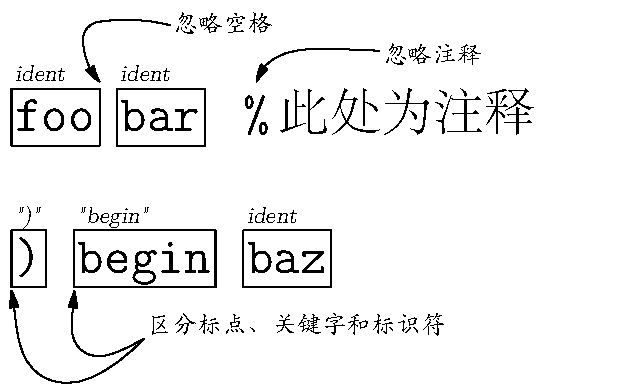
\includegraphics[scale=1.0]{task-of-scanner.pdf}

\caption{扫描器的任务\label{t:x28elem_x22figx2dBx2e1x22x29}}\end{EoplFigure}

扫描器的任务是遍历和分析输入,产生含有这些词条的数据结构。通常的语言中,扫描器可
能是一个过程,在调用时,由输入产生“下一个”词牌。

可以从头写出一个扫描器,但那又麻烦,又易错。更好的方式是写出指定语言的词法规范。
这一任务最常用的语言是\emph{正则表达式} (\emph{regular expressions})。正则表达式语言定
义如下:\index{zzheng4ze2biao3da2shi4@正则表达式|idxdecorator{}{}}
\texMathDisplay{\mathit{R} ::= \mathit{Character} \mid \mathit{RR} \mid \mathit{R} \cup \mathit{R} \mid \neg\mathit{Character}}

每个正则表达式匹配一些字符串。我们可以用归纳法定义每个正则表达式匹配的字符串集合。

\begin{itemize}\atItemizeStart

\item 匹配字符 \texMathInline{c} 的字符串只含字符 \texMathInline{c}。

\item 匹配 \texMathInline{\neg c} 的字符串只含一个 \texMathInline{c} 之外的字符。

\item 匹配 \texMathInline{\mathit{RS}} 的字符串由匹配 \texMathInline{\mathit{R}} 和匹配 \texMathInline{\mathit{S}}
的字符串相接而得。这叫做\emph{串联} (\emph{concatenation})。\index{czhuan4lian2@串联|idxdecorator{}{}}

\item 匹配 \texMathInline{\mathit{R} \cup \mathit{S}} 的字符串匹配 \texMathInline{\mathit{R}} 或
\texMathInline{\mathit{S}}。这有时写作 \texMathInline{\mathit{R} \mid \mathit{S}},
叫做\emph{并联} (\emph{alternation})。\index{bzing4lian2@并联|idxdecorator{}{}}

\item 匹配 \texMathInline{\mathit{R}^{*}} 的字符串由 \texMathInline{n} (\texMathInline{n \geq 0}) 个匹配
\texMathInline{\mathit{R}} 的字符串串联而得。这叫做 \texMathInline{\mathit{R}} 的\emph{克莱尼闭包} (\emph{Kleene
 closure})。
\index{kze4lai2ni2xing1hao4bi4bao1@克莱尼星号(闭包)|idxdecorator{}{}}\end{itemize}

看些例子更有帮助:

\begin{itemize}\atItemizeStart

\item \texMathInline{ab} 只匹配字符串 \Scribtexttt{ab}。

\item \texMathInline{ab \cup cd} 匹配字符串 \Scribtexttt{ab} 或 \Scribtexttt{cd}。

\item \texMathInline{(ab \cup cd)(ab \cup cd \cup ef)} 匹配字符串 \Scribtexttt{abab}、\Scribtexttt{abcd}、
\Scribtexttt{abef}、\Scribtexttt{cdab}、\Scribtexttt{cdcd} 和 \Scribtexttt{cdef}。

\item \texMathInline{(ab)^{*}} 匹配空字符串、\Scribtexttt{ab}、\Scribtexttt{abab}、\Scribtexttt{ababab}、\Scribtexttt{abababab}、
\Scribtexttt{{\hbox{\texttt{.}}}{\hbox{\texttt{.}}}{\hbox{\texttt{.}}}}。

\item \texMathInline{(ab \cup cd)^{*}} 匹配空字符串、\Scribtexttt{ab}、\Scribtexttt{cd}、\Scribtexttt{abab}、\Scribtexttt{abcd}、
\Scribtexttt{cdab}、\Scribtexttt{cdcd}、\Scribtexttt{ababab}、\Scribtexttt{{\hbox{\texttt{.}}}{\hbox{\texttt{.}}}{\hbox{\texttt{.}}}cdcdcd}、\Scribtexttt{{\hbox{\texttt{.}}}{\hbox{\texttt{.}}}{\hbox{\texttt{.}}}}。\end{itemize}

上面的例子解释了不同操作的优先级,所以,\texMathInline{{ab}^{*} \cup cd} 表示 \texMathInline{(a(b^{*}))
\cup (cd)}。

我们例子中的规范可用正则表达式写作

\begin{EoplCodeInset}\begin{SVerbatim}\begin{SingleColumn}\texMathInline{whitespace = (space \cup newline)(space \cup newline)^{*}}\Scribtexttt{}

\Scribtexttt{}\texMathInline{comment = \Scribtexttt{\%}(\neg newline)^{*}}\Scribtexttt{}

\Scribtexttt{}\texMathInline{identifier = letter(letter \cup digit)^{*}}\end{SingleColumn}\end{SVerbatim}\end{EoplCodeInset}

\index{czi2pai2@词牌|(idxdecorator{}{}}
扫描器用正则表达式获取词牌时,规则总是取\emph{最长}匹配。所以 \Scribtexttt{xyz} 扫描为一
个标识符,而非三个。

扫描器找到一个词牌时,它返回的数据结构至少包含下列数据:

\begin{itemize}\atItemizeStart

\item 一个\emph{类别} (\emph{class}),描述词牌的种类。类别的集合是词法规范的一部分。
SLLGEN 使用 Scheme 符号区分这些类别;其他语法分析器可能使用其他数据结构。

\item 一段数据,描述特定词牌。这段数据的性质也是词法规范的一部分。在我们的系统
中,数据如下:标识符的数据是由词牌字符串产生的 Scheme 符号;数字的数据是由数字
字面值描述的数值;字符串字面值的数据就是字符串。字符串数据用作关键字和标点。在
没有符号的实现语言中,可以改用字符串(标识符的名字),或者以标识符为索引的哈希
表(\emph{符号表} (\emph{symbol table}))条目。

\item 一段数据,描述该词牌在输入中的位置。解析器用这一信息帮助程序员定位语法错
误。\end{itemize}

通常,词牌的内部结构只与扫描器和解析器相关,所以我们不再详加介绍。
\index{szao3miao2@扫描|)idxdecorator{}{}}
\index{czi2pai2@词牌|)idxdecorator{}{}}

\Ssubsection{解析}{解析}\label{t:x28part_x22Bx2e2x22x29}

\index{jzie3xi1@解析|(idxdecorator{}{}}
解析过程将词牌序列组织成有层次的语法结构,如表达式,语句和块。这就像用从句组织句
子。语言的语法结构通常由 BNF 定义,也叫做\emph{上下文无
关语法} (\emph{context{-}free grammar})(\SecRefLocal{t:x28part_x22s1x2e1x2e2x22x29}{1.1.2}{语法定义法})。
\index{szhang4xia4wen2wu2guan1yu3fa3@上下文无关语法|idxdecorator{}{}}
\index{yzu3fa3@语法|idxdecorator{}{}}
\index{jzu4fa3lei4bie2@句法类别|idxdecorator{}{}}

\index{czhou1xiang4yu3fa3shu4@抽象语法树|idxdecorator{}{}}解析器输入为词牌序列,输出为一棵抽象语法树
(\SecRefLocal{t:x28part_x22s2x2e5x22x29}{2.5}{抽象语法及其表示})。SLLGEN 生成的抽象语法树可用 \Scribtexttt{define{-}datatype} 描述。
\index{fzei1zhong1jie2fu2@非终结符|(idxdecorator{}{}}
对给定的语法,每个非终结符都对应一个数据类型。以每个非终结符为左边内容的生成式都
对应一个变体。式子右边出现的每个非终结符、标识符和数字都对应变体中的一个字段。
\SecRefLocal{t:x28part_x22s2x2e5x22x29}{2.5}{抽象语法及其表示}有一个简单示例。当语法中有多个非终结符时,可以考虑
\{ex4.22\} 中的语法。
\index{fzei1zhong1jie2fu2@非终结符|)idxdecorator{}{}}


\noindent \begin{Small}\Iidentity{\begin{align*} \mathit{Statement} &::= \Scribtexttt{{\char`\{} }\Iidentity{\mathit{Statement}}\Scribtexttt{ ; }\Iidentity{\mathit{Statement}}\Scribtexttt{ {\char`\}}} \\[-3pt]
                    &::= \Scribtexttt{while }\Iidentity{\mathit{Expression}}\Scribtexttt{ do }\Iidentity{\mathit{Statement}} \\[-3pt]
                    &::= \Iidentity{\mathit{Identifier}}\Scribtexttt{ {\hbox{\texttt{:}}}= }\Iidentity{\mathit{Expression}} \\[-3pt]
\mathit{Expression} &::= \mathit{Identifier} \\[-3pt]
                    &::= \Scribtexttt{(}\Iidentity{\mathit{Expression}}\Scribtexttt{ {-} }\Iidentity{\mathit{Expression}}\Scribtexttt{)}\end{align*}}\end{Small}

这个语法产生的树由如下数据类型描述:

\begin{Subflow}\begin{EoplCodeInset}\begin{SCodeFlow}\begin{RktBlk}\begin{SingleColumn}\RktPn{(}\RktSym{define{-}datatype}\mbox{\hphantom{\Scribtexttt{x}}}\RktSym{statement}\mbox{\hphantom{\Scribtexttt{x}}}\RktSym{statement{\hbox{\texttt{?}}}}

\mbox{\hphantom{\Scribtexttt{xx}}}\RktPn{(}\RktSym{compound{-}statement}

\mbox{\hphantom{\Scribtexttt{xxxx}}}\RktPn{(}\RktSym{stmt1}\mbox{\hphantom{\Scribtexttt{x}}}\RktSym{statement{\hbox{\texttt{?}}}}\RktPn{)}

\mbox{\hphantom{\Scribtexttt{xxxx}}}\RktPn{(}\RktSym{stmt2}\mbox{\hphantom{\Scribtexttt{x}}}\RktSym{statement{\hbox{\texttt{?}}}}\RktPn{)}\RktPn{)}

\mbox{\hphantom{\Scribtexttt{xx}}}\RktPn{(}\RktSym{while{-}statement}

\mbox{\hphantom{\Scribtexttt{xxxx}}}\RktPn{(}\RktSym{test}\mbox{\hphantom{\Scribtexttt{x}}}\RktSym{expression{\hbox{\texttt{?}}}}\RktPn{)}

\mbox{\hphantom{\Scribtexttt{xxxx}}}\RktPn{(}\RktSym{body}\mbox{\hphantom{\Scribtexttt{x}}}\RktSym{statement{\hbox{\texttt{?}}}}\RktPn{)}\RktPn{)}

\mbox{\hphantom{\Scribtexttt{xx}}}\RktPn{(}\RktSym{assign{-}statement}

\mbox{\hphantom{\Scribtexttt{xxxx}}}\RktPn{(}\RktSym{lhs}\mbox{\hphantom{\Scribtexttt{x}}}\RktSym{symbol{\hbox{\texttt{?}}}}\RktPn{)}

\mbox{\hphantom{\Scribtexttt{xxxx}}}\RktPn{(}\RktSym{rhs}\mbox{\hphantom{\Scribtexttt{x}}}\RktSym{expression{\hbox{\texttt{?}}}}\RktPn{)}\RktPn{)}\RktPn{)}

\mbox{\hphantom{\Scribtexttt{x}}}

\RktPn{(}\RktSym{define{-}datatype}\mbox{\hphantom{\Scribtexttt{x}}}\RktSym{expression}\mbox{\hphantom{\Scribtexttt{x}}}\RktSym{expression{\hbox{\texttt{?}}}}

\mbox{\hphantom{\Scribtexttt{xx}}}\RktPn{(}\RktSym{var{-}exp}

\mbox{\hphantom{\Scribtexttt{xxxx}}}\RktPn{(}\RktSym{var}\mbox{\hphantom{\Scribtexttt{x}}}\RktSym{symbol{\hbox{\texttt{?}}}}\RktPn{)}\RktPn{)}

\mbox{\hphantom{\Scribtexttt{xx}}}\RktPn{(}\RktSym{diff{-}exp}

\mbox{\hphantom{\Scribtexttt{xxxx}}}\RktPn{(}\RktSym{exp1}\mbox{\hphantom{\Scribtexttt{x}}}\RktSym{expression{\hbox{\texttt{?}}}}\RktPn{)}

\mbox{\hphantom{\Scribtexttt{xxxx}}}\RktPn{(}\RktSym{exp2}\mbox{\hphantom{\Scribtexttt{x}}}\RktSym{expression{\hbox{\texttt{?}}}}\RktPn{)}\RktPn{)}\RktPn{)}\end{SingleColumn}\end{RktBlk}\end{SCodeFlow}\end{EoplCodeInset}

式子右边的每个非终结符对应的树作为一个字段;标识符对应的符号作为一个字段。变体名
字在用 SLLGEN 写语法时指定。字段名是自动生成的;这里,我们给字段起了一些便于记忆
的名字。例如,输入

\begin{EoplCodeInset}\begin{SVerbatim}\begin{SingleColumn}\Scribtexttt{{\char`\{}x {\hbox{\texttt{:}}}= foo; while x do x {\hbox{\texttt{:}}}= (x {-} bar){\char`\}}}\end{SingleColumn}\end{SVerbatim}\end{EoplCodeInset}

产生输出

\begin{EoplCodeInset}\begin{SCodeFlow}\begin{RktBlk}\begin{SingleColumn}\RktVal{\#}\RktVal{(}\RktVal{struct{\hbox{\texttt{:}}}compound{-}statement}

\mbox{\hphantom{\Scribtexttt{xxx}}}\RktVal{\#}\RktVal{(}\RktVal{struct{\hbox{\texttt{:}}}assign{-}statement}\mbox{\hphantom{\Scribtexttt{x}}}\RktVal{x}\mbox{\hphantom{\Scribtexttt{x}}}\RktVal{\#}\RktVal{(}\RktVal{struct{\hbox{\texttt{:}}}var{-}exp}\mbox{\hphantom{\Scribtexttt{x}}}\RktVal{foo}\RktVal{)}\RktVal{)}

\mbox{\hphantom{\Scribtexttt{xxx}}}\RktVal{\#}\RktVal{(}\RktVal{struct{\hbox{\texttt{:}}}while{-}statement}

\mbox{\hphantom{\Scribtexttt{xxxxxx}}}\RktVal{\#}\RktVal{(}\RktVal{struct{\hbox{\texttt{:}}}var{-}exp}\mbox{\hphantom{\Scribtexttt{x}}}\RktVal{x}\RktVal{)}

\mbox{\hphantom{\Scribtexttt{xxxxxx}}}\RktVal{\#}\RktVal{(}\RktVal{struct{\hbox{\texttt{:}}}assign{-}statement}\mbox{\hphantom{\Scribtexttt{x}}}\RktVal{x}

\mbox{\hphantom{\Scribtexttt{xxxxxxxxx}}}\RktVal{\#}\RktVal{(}\RktVal{struct{\hbox{\texttt{:}}}diff{-}exp}

\mbox{\hphantom{\Scribtexttt{xxxxxxxxxxxx}}}\RktVal{\#}\RktVal{(}\RktVal{struct{\hbox{\texttt{:}}}var{-}exp}\mbox{\hphantom{\Scribtexttt{x}}}\RktVal{x}\RktVal{)}

\mbox{\hphantom{\Scribtexttt{xxxxxxxxxxxx}}}\RktVal{\#}\RktVal{(}\RktVal{struct{\hbox{\texttt{:}}}var{-}exp}\mbox{\hphantom{\Scribtexttt{x}}}\RktVal{bar}\RktVal{)}\RktVal{)}\RktVal{)}\RktVal{)}\RktVal{)}\end{SingleColumn}\end{RktBlk}\end{SCodeFlow}

\noindent \index{jzie3xi1@解析|)idxdecorator{}{}}\end{EoplCodeInset}\end{Subflow}

\Ssubsection{SLLGEN 中的扫描器和解析器}{SLLGEN 中的扫描器和解析器}\label{t:x28part_x22Bx2e3x22x29}



\Ssubsubsectionstarx{定义扫描器}{定义扫描器}\label{t:x28part_x22Bx2e3x2dscannersx22x29}

\index{szao3miao2@扫描|(idxdecorator{}{}}
在 SLLGEN 中,扫描器用正则表达式定义。我们的例子用 SLLGEN,要写成下面这样:

\begin{EoplCodeInset}\begin{SCodeFlow}\begin{RktBlk}\begin{SingleColumn}\RktPn{(}\RktSym{define}\mbox{\hphantom{\Scribtexttt{x}}}\RktSym{scanner{-}spec{-}a}

\mbox{\hphantom{\Scribtexttt{xx}}}\RktVal{{\textquotesingle}}\RktVal{(}\RktVal{(}\RktVal{white{-}sp}\mbox{\hphantom{\Scribtexttt{x}}}\RktVal{(}\RktVal{whitespace}\RktVal{)}\mbox{\hphantom{\Scribtexttt{x}}}\RktVal{skip}\RktVal{)}

\mbox{\hphantom{\Scribtexttt{xxxx}}}\RktVal{(}\RktVal{comment}\mbox{\hphantom{\Scribtexttt{x}}}\RktVal{(}\RktVal{"\%"}\mbox{\hphantom{\Scribtexttt{x}}}\RktVal{(}\RktVal{arbno}\mbox{\hphantom{\Scribtexttt{x}}}\RktVal{(}\RktVal{not}\mbox{\hphantom{\Scribtexttt{x}}}\RktVal{\#{\char`\\}newline}\RktVal{)}\RktVal{)}\RktVal{)}\mbox{\hphantom{\Scribtexttt{x}}}\RktVal{skip}\RktVal{)}

\mbox{\hphantom{\Scribtexttt{xxxx}}}\RktVal{(}\RktVal{identifier}\mbox{\hphantom{\Scribtexttt{x}}}\RktVal{(}\RktVal{letter}\mbox{\hphantom{\Scribtexttt{x}}}\RktVal{(}\RktVal{arbno}\mbox{\hphantom{\Scribtexttt{x}}}\RktVal{(}\RktVal{or}\mbox{\hphantom{\Scribtexttt{x}}}\RktVal{letter}\mbox{\hphantom{\Scribtexttt{x}}}\RktVal{digit}\RktVal{)}\RktVal{)}\RktVal{)}\mbox{\hphantom{\Scribtexttt{x}}}\RktVal{symbol}\RktVal{)}

\mbox{\hphantom{\Scribtexttt{xxxx}}}\RktVal{(}\RktVal{number}\mbox{\hphantom{\Scribtexttt{x}}}\RktVal{(}\RktVal{digit}\mbox{\hphantom{\Scribtexttt{x}}}\RktVal{(}\RktVal{arbno}\mbox{\hphantom{\Scribtexttt{x}}}\RktVal{digit}\RktVal{)}\RktVal{)}\mbox{\hphantom{\Scribtexttt{x}}}\RktVal{number}\RktVal{)}\RktVal{)}\RktPn{)}\end{SingleColumn}\end{RktBlk}\end{SCodeFlow}\end{EoplCodeInset}

如果扫描器要和处理关键字或标点(如 \Scribtexttt{while} 或 \Scribtexttt{=})的解析器共用,不需要手
动将这些放入扫描器中;解析器生成器会自动添加它们。

SLLGEN 中的扫描器定义是满足如下语法的列表:

\begin{Small}\Iidentity{\begin{align*}            \mathit{Scanner\mbox{-}spec} &::= \Scribtexttt{(}\Iidentity{\{\mathit{Regexp\mbox{-}and\mbox{-}action}\}^{*}}\Scribtexttt{)} \\[-3pt]
\mathit{Regexp\mbox{-}and\mbox{-}action} &::= \Scribtexttt{(}\Iidentity{\mathit{Name}}\Scribtexttt{ (}\Iidentity{\{\mathit{Regexp}\}^{*}}\Scribtexttt{) }\Iidentity{\mathit{Action}}\Scribtexttt{)} \\[-3pt]
                           \mathit{Name} &::= \mathit{Symbol} \\[-3pt]
                         \mathit{Regexp} &::= \mathit{String} \mid \Scribtexttt{letter} \mid \Scribtexttt{digit} \mid \Scribtexttt{whitespace} \mid \Scribtexttt{any} \\[-3pt]
                                         &::= \Scribtexttt{(not }\Iidentity{\mathit{Character}}\Scribtexttt{)} \mid \Scribtexttt{(or }\Iidentity{\{\mathit{Regexp}\}^{*}}\Scribtexttt{)} \\[-3pt]
                                         &::= \Scribtexttt{(arbno }\Iidentity{\mathit{Regexp}}\Scribtexttt{)} \mid \Scribtexttt{(concat }\Iidentity{\{\mathit{Regexp}\}^{*}}\Scribtexttt{)} \\[-3pt]
                         \mathit{Action} &::= \Scribtexttt{skip} \mid \Scribtexttt{symbol} \mid \Scribtexttt{number} \mid \Scribtexttt{string}\end{align*}}\end{Small}

列表中的每一项都定义了一个正则表达式,定义包含名字、一系列正则表达式,以及匹配成
功时的动作。名字是一个 Scheme 符号,表示词牌的类别。

由于扫描器中的顶层\emph{正则表达式} (\emph{regexp}) 几乎总是串联而得,定义的第二部分是
一系列正则表达式。正则表达式可以是一个字符串;可以是预先定义的四个测试器之一:
\Scribtexttt{letter}(匹配任何字母),\Scribtexttt{digit}(匹配任何数字),\Scribtexttt{whitespace}(匹配任
何 Scheme 空白字符),以及 \Scribtexttt{any}(匹配任意字符);可以是一个去反字符;也可以
是组合而得的正则表达式,采用 Scheme 式的语法,以 \Scribtexttt{or} 表示并联,以
\Scribtexttt{concat} 表示串联,以 \Scribtexttt{arbno} 表示克莱尼星号。

扫描器工作时,把字符收集到一个缓存中。当扫描器断定找出了定义中所有正则表达式的最
长匹配时,它执行对应正则表达式的\emph{动作}。

动作为下列之一:

\begin{itemize}\atItemizeStart

\item 符号 \Scribtexttt{skip}。这表示词牌结束,但不产生任何词牌。扫描器继续处理字符串,
找出下一个词牌。这一动作用于空白字符和注释。

\item 符号 \Scribtexttt{symbol}。缓存中的字符转换为一个 Scheme 符号,并产生一个词牌,以
指定类别名为其类别,以对应符号为其数据。

\item 符号 \Scribtexttt{number}。缓存中的字符转换为一个 Scheme 数值,并产生一个词牌,以
指定类别名为其类别,以对应数值为其数据。

\item 符号 \Scribtexttt{string}。缓存中的字符转换为一个 Scheme 字符串,并产生一个词牌,
以指定类别名为其类别,以对应字符串为其数据。\end{itemize}

如果两个正则表达式同时为最长匹配,\Scribtexttt{string} 优先于 \Scribtexttt{symbol}。这条规则意味着
关键字会按关键字处理,而非标识符。
\index{szao3miao2@扫描|)idxdecorator{}{}}

\Ssubsubsectionstarx{定义语法}{定义语法}\label{t:x28part_x22Bx2e3x2dgrammarsx22x29}

\index{jzie3xi1@解析|(idxdecorator{}{}}
SLLGEN 还包含一种定义语法的语言。上面的简单语法用 SLLGEN 写作

\begin{EoplCodeInset}\begin{SCodeFlow}\begin{RktBlk}\begin{SingleColumn}\RktPn{(}\RktSym{define}\mbox{\hphantom{\Scribtexttt{x}}}\RktSym{grammar{-}a1}

\mbox{\hphantom{\Scribtexttt{xx}}}\RktVal{{\textquotesingle}}\RktVal{(}\RktVal{(}\RktVal{statement}

\mbox{\hphantom{\Scribtexttt{xxxxxx}}}\RktVal{(}\RktVal{"{\char`\{}"}\mbox{\hphantom{\Scribtexttt{x}}}\RktVal{statement}\mbox{\hphantom{\Scribtexttt{x}}}\RktVal{";"}\mbox{\hphantom{\Scribtexttt{x}}}\RktVal{statement}\mbox{\hphantom{\Scribtexttt{x}}}\RktVal{"{\char`\}}"}\RktVal{)}

\mbox{\hphantom{\Scribtexttt{xxxxxx}}}\RktVal{compound{-}statement}\RktVal{)}

\mbox{\hphantom{\Scribtexttt{xxxx}}}\RktVal{(}\RktVal{statement}

\mbox{\hphantom{\Scribtexttt{xxxxxx}}}\RktVal{(}\RktVal{"while"}\mbox{\hphantom{\Scribtexttt{x}}}\RktVal{expression}\mbox{\hphantom{\Scribtexttt{x}}}\RktVal{"do"}\mbox{\hphantom{\Scribtexttt{x}}}\RktVal{statement}\RktVal{)}

\mbox{\hphantom{\Scribtexttt{xxxxxx}}}\RktVal{while{-}statement}\RktVal{)}

\mbox{\hphantom{\Scribtexttt{xxxx}}}\RktVal{(}\RktVal{statement}

\mbox{\hphantom{\Scribtexttt{xxxxxx}}}\RktVal{(}\RktVal{identifier}\mbox{\hphantom{\Scribtexttt{x}}}\RktVal{"{\hbox{\texttt{:}}}="}\mbox{\hphantom{\Scribtexttt{x}}}\RktVal{expression}\RktVal{)}

\mbox{\hphantom{\Scribtexttt{xxxxxx}}}\RktVal{assign{-}statement}\RktVal{)}

\mbox{\hphantom{\Scribtexttt{xxxx}}}\RktVal{(}\RktVal{expression}

\mbox{\hphantom{\Scribtexttt{xxxxxx}}}\RktVal{(}\RktVal{identifier}\RktVal{)}

\mbox{\hphantom{\Scribtexttt{xxxxxx}}}\RktVal{var{-}exp}\RktVal{)}

\mbox{\hphantom{\Scribtexttt{xxxx}}}\RktVal{(}\RktVal{expression}

\mbox{\hphantom{\Scribtexttt{xxxxxx}}}\RktVal{(}\RktVal{"("}\mbox{\hphantom{\Scribtexttt{x}}}\RktVal{expression}\mbox{\hphantom{\Scribtexttt{x}}}\RktVal{"{-}"}\mbox{\hphantom{\Scribtexttt{x}}}\RktVal{expression}\mbox{\hphantom{\Scribtexttt{x}}}\RktVal{")"}\RktVal{)}

\mbox{\hphantom{\Scribtexttt{xxxxxx}}}\RktVal{diff{-}exp}\RktVal{)}\RktVal{)}\RktPn{)}\end{SingleColumn}\end{RktBlk}\end{SCodeFlow}\end{EoplCodeInset}

SLLGEN 中的语法是由下列语法描述的列表:

\begin{Small}\index{yzu3fa3sheng1cheng2shi4@语法生成式|idxdecorator{}{}}
\Iidentity{\begin{align*}          \mathit{Grammar} &::= \Scribtexttt{(}\Iidentity{\{\mathit{Production}\}^{*}}\Scribtexttt{)} \\[-3pt]
       \mathit{Production} &::= \Scribtexttt{(}\Iidentity{\mathit{Lhs}}\Scribtexttt{ (}\Iidentity{\{\mathit{Rhs\mbox{-}item}\}^{*}}\Scribtexttt{) }\Iidentity{\mathit{Prod\mbox{-}name}}\Scribtexttt{)} \\[-3pt]
             \mathit{Lhs} &::= \mathit{Symbol} \\[-3pt]
 \mathit{Rhs\mbox{-}item} &::= \mathit{Symbol} \mid \mathit{String} \\[-3pt]
                          &::= \Scribtexttt{(arbno }\Iidentity{\mathit{\{Rhs\mbox{-}item\}^{*}}}\Scribtexttt{)} \\[-3pt]
                          &::= \Scribtexttt{(separated{-}list }\Iidentity{\mathit{\{Rhs\mbox{-}item\}^{*}}}\Scribtexttt{ }\Iidentity{\mathit{String}}\Scribtexttt{)} \\[-3pt]
\mathit{Prod\mbox{-}name} &::= \mathit{Symbol}\end{align*}}\end{Small}

语法是生成式列表。第一个生成式的左边是语法的起始符号。每个生成式包含左边(一个非
终结符号)、右边(\texMathInline{rhs\mbox{-}item} 的列表),以及生成式名字。生成式的右边是符
号或者字符串列表。符号是非终结符;字符串是字符串字面值。式子右边也可以包含
\Scribtexttt{arbno} 或 \Scribtexttt{separated{-}list};这些留待下面讨论。生成式的名字是一个符号,成
为 \Scribtexttt{define{-}datatype} 中对应生成式的变体名。

在 SLLGEN 中,解析器必须在仅获知以下内容的条件下,通过语法断定生成式:(1) 正在寻
找哪一非终结符,(2) 正在解析的字符串中的首个符号(词牌)。这种形式的语法叫做
\texMathInline{LL(1)} 语法;SLLGEN 表示 Scheme \texMathInline{LL(1)} 解析器\textbf{生成}器(Scheme
\texMathInline{LL(1)} parser GENerator)。在实践中,这有些过于严格了,但足以应付本书需要。如
果输入语法不满足这一条件,SLLGEN 会给出一条警告。

\Ssubsubsectionstarx{SLLGEN的操作}{SLLGEN的操作}\label{t:x28part_x22Bx2e3x2doperationsx22x29}

SLLGEN 包含几个过程,将扫描器和语法结合起来,形成可以执行的解析器。
 展示了用 SLLGEN 定义语言扫描器和解析器的例子。

过程 \Scribtexttt{sllgen{\hbox{\texttt{:}}}make{-}define{-}datatypes} 负责为语法的每个生成式产生一个
\Scribtexttt{define{-}datatype} 表达式,供 \Scribtexttt{cases} 使用。过程
\Scribtexttt{sllgen{\hbox{\texttt{:}}}list{-}define{-}datatypes} 也生成 \Scribtexttt{define{-}datatype} 表达式,但是会以列
表形式返回,而非执行它们。由这些过程生成的字段名不够直观,因为语法中没有这些信息;
要得到更好的字段名,需要写出 \Scribtexttt{define{-}datatype}。

过程 \Scribtexttt{sllgen{\hbox{\texttt{:}}}make{-}string{-}scanner} 取一扫描器和一语法,生成一个扫描过程。得出
的过程可以处理一个字符串,得到一个词牌列表。语法用来给得到的扫描过程添加关键字。
这一过程主要用于调试。

过程 \Scribtexttt{sllgen{\hbox{\texttt{:}}}make{-}string{-}parser} 生成一个解析器。解析器是一过程,它取一字符串,
用扫描器扫描它,用语法解析它,然后返回一棵抽象语法树。像
\Scribtexttt{sllgen{\hbox{\texttt{:}}}make{-}string{-}scanner} 一样,语法中的字符串字面值包含在扫描器中。

SLLGEN 也可以用来生成读入{-}求值{-}打印循环(\SecRefLocal{t:x28part_x22s3x2e1x22x29}{3.1}{规范和实现策略})。过程
\Scribtexttt{sllgen{\hbox{\texttt{:}}}make{-}stream{-}parser} 与字符串版本类似,但是它的输入是字符流,输出是词
牌流。过程 \Scribtexttt{sllgen{\hbox{\texttt{:}}}make{-}rep{-}loop} 取一字符串,一个单参数过程,一个流式解析器,
生成一个读入{-}求值{-}打印循环,以指定字符串为标准输出中的提示符,从标准输入读入字符,
解析它们,然后以指定过程处理抽象语法树,将结果打印出来。例如:

\begin{EoplFigure}[!t]

\begin{SCodeFlow}\begin{RktBlk}\begin{SingleColumn}\RktPn{(}\RktSym{define}\mbox{\hphantom{\Scribtexttt{x}}}\RktSym{scanner{-}spec{-}1}\mbox{\hphantom{\Scribtexttt{x}}}\RktSym{{\hbox{\texttt{.}}}{\hbox{\texttt{.}}}{\hbox{\texttt{.}}}}\RktPn{)}

\mbox{\hphantom{\Scribtexttt{x}}}

\RktPn{(}\RktSym{define}\mbox{\hphantom{\Scribtexttt{x}}}\RktSym{grammar{-}1}\mbox{\hphantom{\Scribtexttt{x}}}\RktSym{{\hbox{\texttt{.}}}{\hbox{\texttt{.}}}{\hbox{\texttt{.}}}}\RktPn{)}

\mbox{\hphantom{\Scribtexttt{x}}}

\RktPn{(}\RktSym{sllgen{\hbox{\texttt{:}}}make{-}define{-}datatypes}\mbox{\hphantom{\Scribtexttt{x}}}\RktSym{scanner{-}spec{-}1}\mbox{\hphantom{\Scribtexttt{x}}}\RktSym{grammar{-}1}\RktPn{)}

\mbox{\hphantom{\Scribtexttt{x}}}

\RktPn{(}\RktSym{define}\mbox{\hphantom{\Scribtexttt{x}}}\RktSym{list{-}the{-}datatypes}

\mbox{\hphantom{\Scribtexttt{xx}}}\RktPn{(}\RktSym{lambda}\mbox{\hphantom{\Scribtexttt{x}}}\RktPn{(}\RktPn{)}

\mbox{\hphantom{\Scribtexttt{xxxx}}}\RktPn{(}\RktSym{sllgen{\hbox{\texttt{:}}}list{-}define{-}datatypes}\mbox{\hphantom{\Scribtexttt{x}}}\RktSym{scanner{-}spec{-}1}\mbox{\hphantom{\Scribtexttt{x}}}\RktSym{grammar{-}1}\RktPn{)}\RktPn{)}\RktPn{)}

\mbox{\hphantom{\Scribtexttt{x}}}

\RktPn{(}\RktSym{define}\mbox{\hphantom{\Scribtexttt{x}}}\RktSym{just{-}scan}

\mbox{\hphantom{\Scribtexttt{xx}}}\RktPn{(}\RktSym{sllgen{\hbox{\texttt{:}}}make{-}string{-}scanner}\mbox{\hphantom{\Scribtexttt{x}}}\RktSym{scanner{-}spec{-}1}\mbox{\hphantom{\Scribtexttt{x}}}\RktSym{grammar{-}1}\RktPn{)}\RktPn{)}

\mbox{\hphantom{\Scribtexttt{x}}}

\RktPn{(}\RktSym{define}\mbox{\hphantom{\Scribtexttt{x}}}\RktSym{scan\&parse}

\mbox{\hphantom{\Scribtexttt{xx}}}\RktPn{(}\RktSym{sllgen{\hbox{\texttt{:}}}make{-}string{-}parser}\mbox{\hphantom{\Scribtexttt{x}}}\RktSym{scanner{-}spec{-}1}\mbox{\hphantom{\Scribtexttt{x}}}\RktSym{grammar{-}1}\RktPn{)}\RktPn{)}

\mbox{\hphantom{\Scribtexttt{x}}}

\RktPn{(}\RktSym{define}\mbox{\hphantom{\Scribtexttt{x}}}\RktSym{read{-}eval{-}print}

\mbox{\hphantom{\Scribtexttt{xx}}}\RktPn{(}\RktSym{sllgen{\hbox{\texttt{:}}}make{-}rep{-}loop}\mbox{\hphantom{\Scribtexttt{x}}}\RktVal{"{-}{-}{\Stttextmore} "}\mbox{\hphantom{\Scribtexttt{x}}}\RktSym{value{-}of{-}{-}program}

\mbox{\hphantom{\Scribtexttt{xxxx}}}\RktPn{(}\RktSym{sllgen{\hbox{\texttt{:}}}make{-}stream{-}parser}\mbox{\hphantom{\Scribtexttt{x}}}\RktSym{scanner{-}spec{-}1}\mbox{\hphantom{\Scribtexttt{x}}}\RktSym{grammar{-}1}\RktPn{)}\RktPn{)}\RktPn{)}\end{SingleColumn}\end{RktBlk}\end{SCodeFlow}

\caption{使用 SLLGEN\label{t:x28elem_x22figx2dBx2e2x22x29}}\end{EoplFigure}

\begin{EoplCodeInset}\begin{SVerbatim}\begin{SingleColumn}\Scribtexttt{{\Stttextmore} (define read{-}eval{-}print}

\Scribtexttt{}\mbox{\hphantom{\Scribtexttt{xxxx}}}\Scribtexttt{(sllgen{\hbox{\texttt{:}}}make{-}rep{-}loop "{-}{-}{\Stttextmore} " eval{-}program}

\Scribtexttt{}\mbox{\hphantom{\Scribtexttt{xxxxxx}}}\Scribtexttt{(sllgen{\hbox{\texttt{:}}}make{-}stream{-}parser}

\Scribtexttt{}\mbox{\hphantom{\Scribtexttt{xxxxxxxx}}}\Scribtexttt{scanner{-}spec{-}3{-}1}

\Scribtexttt{}\mbox{\hphantom{\Scribtexttt{xxxxxxxx}}}\Scribtexttt{grammar{-}3{-}1)))}

\Scribtexttt{{\Stttextmore} (read{-}eval{-}print)}

\Scribtexttt{{-}{-}{\Stttextmore} 5}

\Scribtexttt{5}

\Scribtexttt{{-}{-}{\Stttextmore} add1(2)}

\Scribtexttt{3}

\Scribtexttt{{-}{-}{\Stttextmore} +(add1(2),{-}(6,4))}

\Scribtexttt{5}\end{SingleColumn}\end{SVerbatim}\end{EoplCodeInset}

控制流程从这一循环返回 Scheme 读入{-}求值{-}打印循环的方式由系统决定。

\Ssubsubsectionstarx{\Scribtexttt{arbno}
和 \Scribtexttt{separated{-}list} 模板关键字}{\Scribtexttt{arbno}
和 \Scribtexttt{separated{-}list} 模板关键字}\label{t:x28part_x22Bx2e3x2darbnox22x29}

\Scribtexttt{arbno} 关键字即语法中的克莱尼星号:它匹配重复任意次数的条目。例如,生成式


\noindent \begin{Small}\texMathDisplay{\mathit{statement} ::= \Scribtexttt{{\char`\{} }\texMathInline{\{statement \Scribtexttt{;}\}^{*}}\Scribtexttt{ {\char`\}}}}\end{Small}

\noindent \begin{Subflow}在 SLLGEN 中可写作

\begin{EoplCodeInset}\begin{SCodeFlow}\begin{RktBlk}\begin{SingleColumn}\RktPn{(}\RktSym{define}\mbox{\hphantom{\Scribtexttt{x}}}\RktSym{grammar{-}a2}

\mbox{\hphantom{\Scribtexttt{xx}}}\RktVal{{\textquotesingle}}\RktVal{(}\RktVal{(}\RktVal{statement}

\mbox{\hphantom{\Scribtexttt{xxxxxx}}}\RktVal{(}\RktVal{"{\char`\{}"}\mbox{\hphantom{\Scribtexttt{x}}}\RktVal{(}\RktVal{arbno}\mbox{\hphantom{\Scribtexttt{x}}}\RktVal{statement}\mbox{\hphantom{\Scribtexttt{x}}}\RktVal{";"}\RktVal{)}\mbox{\hphantom{\Scribtexttt{x}}}\RktVal{"{\char`\}}"}\RktVal{)}

\mbox{\hphantom{\Scribtexttt{xxxxxx}}}\RktVal{compound{-}statement}\RktVal{)}

\mbox{\hphantom{\Scribtexttt{xxxxx}}}\RktVal{{\hbox{\texttt{.}}}{\hbox{\texttt{.}}}{\hbox{\texttt{.}}}}\RktVal{)}\RktPn{)}\end{SingleColumn}\end{RktBlk}\end{SCodeFlow}\end{EoplCodeInset}

这匹配一条复合语句,由任意数量分号分隔的语句序列组成。\end{Subflow}

\Scribtexttt{arbno} 在抽象语法树中对应单个字段。该字段包含一个\emph{列表},由 \Scribtexttt{arbno}
内的非终结符数据组成。我们的例子生成如下数据类型:

\begin{EoplCodeInset}\begin{SCodeFlow}\begin{RktBlk}\begin{SingleColumn}\RktPn{(}\RktSym{define{-}datatype}\mbox{\hphantom{\Scribtexttt{x}}}\RktSym{statement}\mbox{\hphantom{\Scribtexttt{x}}}\RktSym{statement{\hbox{\texttt{?}}}}

\mbox{\hphantom{\Scribtexttt{xx}}}\RktPn{(}\RktSym{compound{-}statement}

\mbox{\hphantom{\Scribtexttt{xxxx}}}\RktPn{(}\RktSym{compound{-}statement32}\mbox{\hphantom{\Scribtexttt{x}}}\RktPn{(}\RktSym{list{-}of}\mbox{\hphantom{\Scribtexttt{x}}}\RktSym{statement{\hbox{\texttt{?}}}}\RktPn{)}\RktPn{)}\RktPn{)}

\mbox{\hphantom{\Scribtexttt{xx}}}\RktSym{{\hbox{\texttt{.}}}{\hbox{\texttt{.}}}{\hbox{\texttt{.}}}}\RktPn{)}\end{SingleColumn}\end{RktBlk}\end{SCodeFlow}\end{EoplCodeInset}

简单交互为:

\begin{EoplCodeInset}\begin{SVerbatim}\begin{SingleColumn}\Scribtexttt{{\Stttextmore} (define scan\&parse2}

\Scribtexttt{}\mbox{\hphantom{\Scribtexttt{xxxx}}}\Scribtexttt{(sllgen{\hbox{\texttt{:}}}make{-}string{-}parser scanner{-}spec{-}a grammar{-}a2))}

\Scribtexttt{}\mbox{\hphantom{\Scribtexttt{x}}}

\Scribtexttt{{\Stttextmore} (scan\&parse2 "{\char`\{}x {\hbox{\texttt{:}}}= foo; y {\hbox{\texttt{:}}}= bar; z {\hbox{\texttt{:}}}= uu;{\char`\}}")}

\Scribtexttt{(compound{-}statement}

\Scribtexttt{}\mbox{\hphantom{\Scribtexttt{xx}}}\Scribtexttt{((assign{-}statement x (var{-}exp foo))}

\Scribtexttt{}\mbox{\hphantom{\Scribtexttt{xxx}}}\Scribtexttt{(assign{-}statement y (var{-}exp bar))}

\Scribtexttt{}\mbox{\hphantom{\Scribtexttt{xxx}}}\Scribtexttt{(assign{-}statement z (var{-}exp uu))))}\end{SingleColumn}\end{SVerbatim}\end{EoplCodeInset}

我们可以把非终结符序列放入 \Scribtexttt{arbno} 中。这时,节点中会有多个字段,每个对应一个
非终结符;每个字段包含一个语法树列表。例如:

\begin{EoplCodeInset}\begin{SCodeFlow}\begin{RktBlk}\begin{SingleColumn}\RktPn{(}\RktSym{define}\mbox{\hphantom{\Scribtexttt{x}}}\RktSym{grammar{-}a3}

\mbox{\hphantom{\Scribtexttt{xx}}}\RktVal{{\textquotesingle}}\RktVal{(}\RktVal{(}\RktVal{expression}\mbox{\hphantom{\Scribtexttt{x}}}\RktVal{(}\RktVal{identifier}\RktVal{)}\mbox{\hphantom{\Scribtexttt{x}}}\RktVal{var{-}exp}\RktVal{)}

\mbox{\hphantom{\Scribtexttt{xxxx}}}\RktVal{(}\RktVal{expression}

\mbox{\hphantom{\Scribtexttt{xxxxxx}}}\RktVal{(}\RktVal{"let"}\mbox{\hphantom{\Scribtexttt{x}}}\RktVal{(}\RktVal{arbno}\mbox{\hphantom{\Scribtexttt{x}}}\RktVal{identifier}\mbox{\hphantom{\Scribtexttt{x}}}\RktVal{"="}\mbox{\hphantom{\Scribtexttt{x}}}\RktVal{expression}\RktVal{)}\mbox{\hphantom{\Scribtexttt{x}}}\RktVal{"in"}\mbox{\hphantom{\Scribtexttt{x}}}\RktVal{expression}\RktVal{)}

\mbox{\hphantom{\Scribtexttt{xxxxxx}}}\RktVal{let{-}exp}\RktVal{)}\RktVal{)}\RktPn{)}

\mbox{\hphantom{\Scribtexttt{x}}}

\RktPn{(}\RktSym{define}\mbox{\hphantom{\Scribtexttt{x}}}\RktSym{scan\&parse3}

\mbox{\hphantom{\Scribtexttt{xx}}}\RktPn{(}\RktSym{sllgen{\hbox{\texttt{:}}}make{-}string{-}parser}\mbox{\hphantom{\Scribtexttt{x}}}\RktSym{scanner{-}spec{-}a}\mbox{\hphantom{\Scribtexttt{x}}}\RktSym{grammar{-}a3}\RktPn{)}\RktPn{)}\end{SingleColumn}\end{RktBlk}\end{SCodeFlow}\end{EoplCodeInset}

生成数据类型

\begin{EoplCodeInset}\begin{SCodeFlow}\begin{RktBlk}\begin{SingleColumn}\RktPn{(}\RktSym{define{-}datatype}\mbox{\hphantom{\Scribtexttt{x}}}\RktSym{expression}\mbox{\hphantom{\Scribtexttt{x}}}\RktSym{expression{\hbox{\texttt{?}}}}

\mbox{\hphantom{\Scribtexttt{xx}}}\RktPn{(}\RktSym{var{-}exp}\mbox{\hphantom{\Scribtexttt{x}}}\RktPn{(}\RktSym{var{-}exp4}\mbox{\hphantom{\Scribtexttt{x}}}\RktSym{symbol{\hbox{\texttt{?}}}}\RktPn{)}\RktPn{)}

\mbox{\hphantom{\Scribtexttt{xx}}}\RktPn{(}\RktSym{let{-}exp}

\mbox{\hphantom{\Scribtexttt{xxxx}}}\RktPn{(}\RktSym{let{-}exp9}\mbox{\hphantom{\Scribtexttt{x}}}\RktPn{(}\RktSym{list{-}of}\mbox{\hphantom{\Scribtexttt{x}}}\RktSym{symbol{\hbox{\texttt{?}}}}\RktPn{)}\RktPn{)}

\mbox{\hphantom{\Scribtexttt{xxxx}}}\RktPn{(}\RktSym{let{-}exp7}\mbox{\hphantom{\Scribtexttt{x}}}\RktPn{(}\RktSym{list{-}of}\mbox{\hphantom{\Scribtexttt{x}}}\RktSym{expression{\hbox{\texttt{?}}}}\RktPn{)}\RktPn{)}

\mbox{\hphantom{\Scribtexttt{xxxx}}}\RktPn{(}\RktSym{let{-}exp8}\mbox{\hphantom{\Scribtexttt{x}}}\RktSym{expression{\hbox{\texttt{?}}}}\RktPn{)}\RktPn{)}\RktPn{)}\end{SingleColumn}\end{RktBlk}\end{SCodeFlow}\end{EoplCodeInset}

这里是运用该语法的例子:

\begin{Subflow}\begin{EoplCodeInset}\begin{SVerbatim}\begin{SingleColumn}\Scribtexttt{{\Stttextmore} (scan\&parse3 "let x = y u = v in z")}

\Scribtexttt{(let{-}exp}

\Scribtexttt{}\mbox{\hphantom{\Scribtexttt{xx}}}\Scribtexttt{(x u)}

\Scribtexttt{}\mbox{\hphantom{\Scribtexttt{xx}}}\Scribtexttt{((var{-}exp y) (var{-}exp v))}

\Scribtexttt{}\mbox{\hphantom{\Scribtexttt{xx}}}\Scribtexttt{(var{-}exp z))}\end{SingleColumn}\end{SVerbatim}\end{EoplCodeInset}

定义 \Scribtexttt{(arbno identifier "=" expression)} 生成两个列表:标识符列表和表达式列表。
这很方便,因为我们的解释器能直接从中取出一部分表达式。\end{Subflow}

对某些语言的语法,在列表中只用分隔符,而不用结束符会更方便。这十分常见,因此
SLLGEN 内置这种操作。我们可以写

\begin{EoplCodeInset}\begin{SCodeFlow}\begin{RktBlk}\begin{SingleColumn}\RktPn{(}\RktSym{define}\mbox{\hphantom{\Scribtexttt{x}}}\RktSym{grammar{-}a4}

\mbox{\hphantom{\Scribtexttt{xx}}}\RktVal{{\textquotesingle}}\RktVal{(}\RktVal{(}\RktVal{statement}

\mbox{\hphantom{\Scribtexttt{xxxxxx}}}\RktVal{(}\RktVal{"{\char`\{}"}\mbox{\hphantom{\Scribtexttt{x}}}\RktVal{(}\RktVal{separated{-}list}\mbox{\hphantom{\Scribtexttt{x}}}\RktVal{statement}\mbox{\hphantom{\Scribtexttt{x}}}\RktVal{";"}\RktVal{)}\mbox{\hphantom{\Scribtexttt{x}}}\RktVal{"{\char`\}}"}\RktVal{)}

\mbox{\hphantom{\Scribtexttt{xxxxxx}}}\RktVal{compound{-}statement}\RktVal{)}

\mbox{\hphantom{\Scribtexttt{xxxxx}}}\RktVal{{\hbox{\texttt{.}}}{\hbox{\texttt{.}}}{\hbox{\texttt{.}}}}\RktVal{)}\RktPn{)}\end{SingleColumn}\end{RktBlk}\end{SCodeFlow}\end{EoplCodeInset}

它生成数据类型

\begin{EoplCodeInset}\begin{SCodeFlow}\begin{RktBlk}\begin{SingleColumn}\RktPn{(}\RktSym{define{-}datatype}\mbox{\hphantom{\Scribtexttt{x}}}\RktSym{statement}\mbox{\hphantom{\Scribtexttt{x}}}\RktSym{statement{\hbox{\texttt{?}}}}

\mbox{\hphantom{\Scribtexttt{xx}}}\RktPn{(}\RktSym{compound{-}statement}

\mbox{\hphantom{\Scribtexttt{xxxx}}}\RktPn{(}\RktSym{compound{-}statement103}\mbox{\hphantom{\Scribtexttt{x}}}\RktPn{(}\RktSym{list{-}of}\mbox{\hphantom{\Scribtexttt{x}}}\RktSym{statement{\hbox{\texttt{?}}}}\RktPn{)}\RktPn{)}\RktPn{)}

\mbox{\hphantom{\Scribtexttt{xx}}}\RktSym{{\hbox{\texttt{.}}}{\hbox{\texttt{.}}}{\hbox{\texttt{.}}}}\RktPn{)}\end{SingleColumn}\end{RktBlk}\end{SCodeFlow}\end{EoplCodeInset}

这是简单交互的例子:

\begin{Subflow}\begin{EoplCodeInset}\begin{SVerbatim}\begin{SingleColumn}\Scribtexttt{{\Stttextmore} (define scan\&parse4}

\Scribtexttt{}\mbox{\hphantom{\Scribtexttt{xxxx}}}\Scribtexttt{(sllgen{\hbox{\texttt{:}}}make{-}string{-}parser scanner{-}spec{-}a grammar{-}a4))}

\Scribtexttt{{\Stttextmore} (scan\&parse4 "{\char`\{}{\char`\}}")}

\Scribtexttt{(compound{-}statement ())}

\Scribtexttt{{\Stttextmore} (scan\&parse4 "{\char`\{}x{\hbox{\texttt{:}}}= y; u {\hbox{\texttt{:}}}= v ; z {\hbox{\texttt{:}}}= t{\char`\}}")}

\Scribtexttt{(compound{-}statement}

\Scribtexttt{}\mbox{\hphantom{\Scribtexttt{xx}}}\Scribtexttt{((assign{-}statement x (var{-}exp y))}

\Scribtexttt{}\mbox{\hphantom{\Scribtexttt{xxx}}}\Scribtexttt{(assign{-}statement u (var{-}exp v))}

\Scribtexttt{}\mbox{\hphantom{\Scribtexttt{xxx}}}\Scribtexttt{(assign{-}statement z (var{-}exp t))))}

\Scribtexttt{{\Stttextmore} (scan\&parse4 "{\char`\{}x{\hbox{\texttt{:}}}= y; u {\hbox{\texttt{:}}}= v ; z {\hbox{\texttt{:}}}= t ;{\char`\}}")}

\Scribtexttt{Error in parsing{\hbox{\texttt{:}}} at line 1}

\Scribtexttt{Nonterminal {\Stttextless}seplist3{\Stttextmore} can{'}t begin with string "{\char`\}}"}\end{SingleColumn}\end{SVerbatim}\end{EoplCodeInset}

在本例中,输入字符串结尾有一个分号,与语法不符,所以报错。\end{Subflow}

类似于 \Scribtexttt{arbno},我们可以在 \Scribtexttt{separated{-}list} 关键字中放置任意非终结符序列。
这时,节点中会有多个字段,每个对应一个非终结符;每个字段包含一个语法树列表。这和
\Scribtexttt{arbno} 生成的数据完全相同;不同的只是具体语法。

我们偶尔会嵌套 \Scribtexttt{arbno} 和 \Scribtexttt{separated{-}list}。\Scribtexttt{arbno} 内的非终结符生成一
个列表,所以 \Scribtexttt{arbno} 内的 \Scribtexttt{arbno} 内的非终结符生成列表的列表。

举个例子,考虑与 \Scribtexttt{grammar{-}a4} 类似的 \Scribtexttt{compound{-}statement},但它支持多赋值:

\begin{EoplCodeInset}\begin{SCodeFlow}\begin{RktBlk}\begin{SingleColumn}\RktPn{(}\RktSym{define}\mbox{\hphantom{\Scribtexttt{x}}}\RktSym{grammar{-}a5}

\mbox{\hphantom{\Scribtexttt{xx}}}\RktVal{{\textquotesingle}}\RktVal{(}\RktVal{(}\RktVal{statement}

\mbox{\hphantom{\Scribtexttt{xxxxxx}}}\RktVal{(}\RktVal{"{\char`\{}"}

\mbox{\hphantom{\Scribtexttt{xxxxxxxx}}}\RktVal{(}\RktVal{separated{-}list}

\mbox{\hphantom{\Scribtexttt{xxxxxxxxxx}}}\RktVal{(}\RktVal{separated{-}list}\mbox{\hphantom{\Scribtexttt{x}}}\RktVal{identifier}\mbox{\hphantom{\Scribtexttt{x}}}\RktVal{","}\RktVal{)}

\mbox{\hphantom{\Scribtexttt{xxxxxxxxxx}}}\RktVal{"{\hbox{\texttt{:}}}="}

\mbox{\hphantom{\Scribtexttt{xxxxxxxxxx}}}\RktVal{(}\RktVal{separated{-}list}\mbox{\hphantom{\Scribtexttt{x}}}\RktVal{expression}\mbox{\hphantom{\Scribtexttt{x}}}\RktVal{","}\RktVal{)}

\mbox{\hphantom{\Scribtexttt{xxxxxxxxxx}}}\RktVal{";"}\RktVal{)}

\mbox{\hphantom{\Scribtexttt{xxxxxxxx}}}\RktVal{"{\char`\}}"}\RktVal{)}

\mbox{\hphantom{\Scribtexttt{xxxxxx}}}\RktVal{compound{-}statement}\RktVal{)}

\mbox{\hphantom{\Scribtexttt{xxxxx}}}\RktVal{(}\RktVal{expression}\mbox{\hphantom{\Scribtexttt{x}}}\RktVal{(}\RktVal{number}\RktVal{)}\mbox{\hphantom{\Scribtexttt{x}}}\RktVal{lit{-}exp}\RktVal{)}

\mbox{\hphantom{\Scribtexttt{xxxxx}}}\RktVal{(}\RktVal{expression}\mbox{\hphantom{\Scribtexttt{x}}}\RktVal{(}\RktVal{identifier}\RktVal{)}\mbox{\hphantom{\Scribtexttt{x}}}\RktVal{var{-}exp}\RktVal{)}\RktVal{)}\RktPn{)}\end{SingleColumn}\end{RktBlk}\end{SCodeFlow}\end{EoplCodeInset}

\begin{EoplCodeInset}\begin{SVerbatim}\begin{SingleColumn}\Scribtexttt{{\Stttextmore} (define scan\&parse5}

\Scribtexttt{}\mbox{\hphantom{\Scribtexttt{xxxx}}}\Scribtexttt{(sllgen{\hbox{\texttt{:}}}make{-}string{-}parser scanner{-}spec{-}a grammar{-}a5))}\end{SingleColumn}\end{SVerbatim}\end{EoplCodeInset}

它为 \Scribtexttt{statement} 生成如下数据类型:

\begin{EoplCodeInset}\begin{SCodeFlow}\begin{RktBlk}\begin{SingleColumn}\RktPn{(}\RktSym{define{-}datatype}\mbox{\hphantom{\Scribtexttt{x}}}\RktSym{statement}\mbox{\hphantom{\Scribtexttt{x}}}\RktSym{statement{\hbox{\texttt{?}}}}

\mbox{\hphantom{\Scribtexttt{xx}}}\RktPn{(}\RktSym{compound{-}statement}

\mbox{\hphantom{\Scribtexttt{xxxx}}}\RktPn{(}\RktSym{compound{-}statement4}\mbox{\hphantom{\Scribtexttt{x}}}\RktPn{(}\RktSym{list{-}of}\mbox{\hphantom{\Scribtexttt{x}}}\RktPn{(}\RktSym{list{-}of}\mbox{\hphantom{\Scribtexttt{x}}}\RktSym{symbol{\hbox{\texttt{?}}}}\RktPn{)}\RktPn{)}\RktPn{)}

\mbox{\hphantom{\Scribtexttt{xxxx}}}\RktPn{(}\RktSym{compound{-}statement3}\mbox{\hphantom{\Scribtexttt{x}}}\RktPn{(}\RktSym{list{-}of}\mbox{\hphantom{\Scribtexttt{x}}}\RktPn{(}\RktSym{list{-}of}\mbox{\hphantom{\Scribtexttt{x}}}\RktSym{expression{\hbox{\texttt{?}}}}\RktPn{)}\RktPn{)}\RktPn{)}\RktPn{)}\RktPn{)}\end{SingleColumn}\end{RktBlk}\end{SCodeFlow}\end{EoplCodeInset}

一般的交互如下:

\begin{EoplCodeInset}\begin{SVerbatim}\begin{SingleColumn}\Scribtexttt{{\Stttextmore} (scan\&parse5 "{\char`\{}x,y {\hbox{\texttt{:}}}= u,v ; z {\hbox{\texttt{:}}}= 4; t1, t2 {\hbox{\texttt{:}}}= 5, 6{\char`\}}")}

\Scribtexttt{(compound{-}statement}

\Scribtexttt{}\mbox{\hphantom{\Scribtexttt{xx}}}\Scribtexttt{((x y) (z) (t1 t2))}

\Scribtexttt{}\mbox{\hphantom{\Scribtexttt{xx}}}\Scribtexttt{(((var{-}exp u) (var{-}exp v))}

\Scribtexttt{}\mbox{\hphantom{\Scribtexttt{xxxx}}}\Scribtexttt{((lit{-}exp 4))}

\Scribtexttt{}\mbox{\hphantom{\Scribtexttt{xxxx}}}\Scribtexttt{((lit{-}exp 5) (lit{-}exp 6))))}\end{SingleColumn}\end{SVerbatim}\end{EoplCodeInset}

这里,\Scribtexttt{compound{-}statement} 有两个字段:标识符列表的列表,对应的表达式列表的列
表。本例中,我们用 \Scribtexttt{separated{-}list} 代替了 \Scribtexttt{arbno},但是 \Scribtexttt{arbno} 也会生
成同样的数据。
\index{jzie3xi1@解析|)idxdecorator{}{}}

\begin{EoplExercise}\label{t:x28elem_x22exBx2e1x22x29}\texMathInline{\textnormal{[}{\star}\textnormal{]}}\mbox{\hphantom{\Scribtexttt{x}}}下列语法按照通常的算术操作符优先级,定义了算术操作表达式:

\Iidentity{\begin{align*}        \mathit{Arith\mbox{-}expr} &::= \mathit{Arith\mbox{-}term} \ \{\mathit{Additive\mbox{-}op}\ \mathit{Arith\mbox{-}term}\}^{*} \\[-3pt]
       \mathit{Arith\mbox{-}term} &::= \mathit{Arith\mbox{-}factor} \ \{\mathit{Multiplicative\mbox{-}op}\ \mathit{Arith\mbox{-}factor}\}^{*} \\[-3pt]
     \mathit{Arith\mbox{-}factor} &::= \mathit{Number} \\[-3pt]
                                  &::= \Scribtexttt{( }\Iidentity{\mathit{Arith\mbox{-}expr}}\Scribtexttt{ )} \\[-3pt]
     \mathit{Additive\mbox{-}op} &::= \Scribtexttt{+} \mid \Scribtexttt{{-}} \\[-3pt]
\mathit{Multiplicative\mbox{-}op} &::= \Scribtexttt{*} \mid \Scribtexttt{/}\end{align*}}

这套语法是说,每个算术表达式都是非空项序列的和;每一项都是非空因数序列的生成式;
每个因数是一个常数或者括号表达式。

用 SLLGEN 写出词法规范和语法,根据这套语法进行扫描和解析。验证这套语法能正确处理
优先级,那么,\Scribtexttt{3+2*66{-}5} 能正确分组为 \texMathInline{3 + (2 \times 66) - 5}。\end{EoplExercise}

\begin{EoplExercise}\label{t:x28elem_x22exBx2e2x22x29}\texMathInline{\textnormal{[}{\star}{\star}\textnormal{]}}\mbox{\hphantom{\Scribtexttt{x}}}上面的语法为什么不能写成 \Scribtexttt{separated{-}list}?\end{EoplExercise}

\begin{EoplExercise}\label{t:x28elem_x22exBx2e3x22x29}\texMathInline{\textnormal{[}{\star}{\star}\textnormal{]}}\mbox{\hphantom{\Scribtexttt{x}}}定义一个解释器,取\{exB.1\} 中解析器生成的抽象语法树,将其当作算术表
达式求值。解析器处理通常的算术操作优先级;但解释器要处理关联性,即,确保同一优先
级(比如加和减)的操作从左向右进行。由于这些表达式中没有变量,解释器不需要取环境
参数。\end{EoplExercise}

\begin{EoplExercise}\label{t:x28elem_x22exBx2e4x22x29}\texMathInline{\textnormal{[}{\star}{\star}\textnormal{]}}\mbox{\hphantom{\Scribtexttt{x}}}扩展前一道练习中的语言和解释器,加入变量。这个新解释器需要环境参数。\end{EoplExercise}

\begin{EoplExercise}\label{t:x28elem_x22exBx2e5x22x29}\texMathInline{\textnormal{[}{\star}\textnormal{]}}\mbox{\hphantom{\Scribtexttt{x}}}给语言和解释器添加单参数操作取反,使之能正确处理输入 \Scribtexttt{3*{-}2}。\end{EoplExercise}

\sectionNewpage

\Ssectionstarx{参考书目}{参考书目}\label{t:x28part_x22bibx22x29}

\begin{BibPara}\index{Abadi, Mart\'{i}n|idxdecorator{}{}}Abadi, Mart\'{i}n, \& \index{Cardelli, Luca|idxdecorator{}{}}Cardelli, Luca. 1996. \emph{A Theory of Objects}. Berlin, Heidelberg,
and New York: Springer{-}Verlag.\end{BibPara}

\begin{BibPara}\index{Abelson, Harold|idxdecorator{}{}}Abelson, Harold, \& \index{Sussman, Gerald Jay|idxdecorator{}{}}Sussman, Gerald Jay. 1985. \emph{The Structure and Interpretation
of Computer Programs}. Cambridge, MA: MIT Press.\end{BibPara}

\begin{BibPara}\index{Abelson, Harold|idxdecorator{}{}}Abelson, Harold, \& \index{Sussman, Gerald Jay|idxdecorator{}{}}Sussman, Gerald Jay. 1996. \emph{Structure and Interpretation of
Computer Programs}. Second edition. Cambridge, MA: McGraw Hill.\end{BibPara}

\begin{BibPara}\index{Aho, Alfred|idxdecorator{}{}}Aho, Alfred V., \index{Lam, Monica|idxdecorator{}{}}Lam, Monica S., \index{Sethi, Ravi|idxdecorator{}{}}Sethi, Ravi, \& \index{Ullman, Jeffrey|idxdecorator{}{}}Ullman, Jeffrey
D. 2006. \emph{Compilers: Principles, Techniques, and Tools}. Second edition. Boston:
Addison{-}Wesley Longman.\end{BibPara}

\begin{BibPara}\index{Appel, Andrew|idxdecorator{}{}}Appel, Andrew W., \& \index{Jim, Trevor|idxdecorator{}{}}Jim, Trevor. 1989. \emph{Continuation{-}Passing, Closure{-}Passing
Style}. Pages 293{--}302 of: Proceedings ACM Symposium on Principles of Programming
Languages.\end{BibPara}

\begin{BibPara}\index{Arnold, Ken|idxdecorator{}{}}Arnold, Ken, \& \index{Gosling, James|idxdecorator{}{}}Gosling, James. 1998. \emph{The Java Programming Language}. Second
edition. The Java Series. Reading, MA: Addison{-}Wesley.\end{BibPara}

\begin{BibPara}\index{Armstrong, Joe|idxdecorator{}{}}Armstrong, Joe. 2007. \emph{Programming Erlang: Software for a Concurrent World}. The
Pragmatic Programmers Publishers.\end{BibPara}

\begin{BibPara}\index{Backus, John|idxdecorator{}{}}Backus, John W., \emph{et al}. 1957. \emph{The Fortran Automatic Coding System}. Pages 188{--}198
of: Western Joint Computer Conference.\end{BibPara}

\begin{BibPara}\index{Barendregt, Henk|idxdecorator{}{}}Barendregt, Henk P. 1981. \emph{The Lambda Calculus: Its Syntax and
Semantics}. Amsterdam: North{-}Holland.\end{BibPara}

\begin{BibPara}\index{Barendregt, Henk|idxdecorator{}{}}Barendregt, Henk P. 1991. \emph{The Lambda Calculus}. Revised edition. Studies in Logic
and the Foundations of Mathematics, no. 103. Amsterdam: North{-}Holland.\end{BibPara}

\begin{BibPara}\index{Bergin, Thomas|idxdecorator{}{}}Bergin, Thomas J., \& \index{Gibson, Richard|idxdecorator{}{}}Gibson, Richard G. (eds.). 1996. \emph{History of Programming
Languages}. New York: Addison{-}Wesley.\end{BibPara}

\begin{BibPara}\index{Birtwistle, Graham|idxdecorator{}{}}Birtwistle, Graham M., \index{Dahl, Ole{-}Johan|idxdecorator{}{}}Dahl, Ole{-}Johan, \& \index{Myhrhaug, Bjorn|idxdecorator{}{}}Myhrhaug, Bjorn. 1973. \emph{Simula Begin}.
Philadelphia: Auerbach.\end{BibPara}

\begin{BibPara}\index{Burstall, Rod|idxdecorator{}{}}Burstall, Rod M. 1969. \emph{Proving Properties of Programs by Structural
Induction}. Computer Journal, \textbf{12}(1), 41{--}48.\end{BibPara}

\begin{BibPara}\index{Church, Alonzo|idxdecorator{}{}}Church, Alonzo. 1941. \emph{The Calculi of Lambda Conversion}. Princeton, NJ: Princeton
University Press. Reprinted 1963 by University Microfilms, Ann Arbor, MI.\end{BibPara}

\begin{BibPara}\index{Clinger, William|idxdecorator{}{}}Clinger, William D., \emph{et al}. 1985a. The Revised Revised Report on Scheme or The
Uncommon Lisp. Technical Memo AIM{-}848. Massachusetts Institute of Technology,
Artificial Intelligence Laboratory.\end{BibPara}

\begin{BibPara}\index{Clinger, William|idxdecorator{}{}}Clinger, William D., \index{Friedman, Daniel|idxdecorator{}{}}Friedman, Daniel P., \& \index{Wand, Mitchell|idxdecorator{}{}}Wand, Mitchell. 1985b. A Scheme for
a Higher{-}Level Semantic Algebra. Pages 237{--}250 of: Reynolds, John, \& Nivat,
Maurice (eds.), \emph{Algebraic Methods in Semantics: Proceedings of the US{-}French
Seminar on the Application of Algebra to Language Definition and Compilation
(Fontainebleau, France, June, 1982)}. Cambridge: Cambridge University Press.\end{BibPara}

\begin{BibPara}\index{Clinger, William|idxdecorator{}{}}Clinger, William D., \index{Rees, Jonathan|idxdecorator{}{}}Rees, Jonathan, \emph{et al}. 1991. The Revised\textsuper{4} Report on the
Algorithmic Language Scheme. \emph{ACM Lisp Pointers}, \textbf{4}(3), 1{--}55.\end{BibPara}

\begin{BibPara}\index{Danvy, Olivier|idxdecorator{}{}}Danvy, Olivier, \& \index{Filinski, Andrzej|idxdecorator{}{}}Filinski, Andrzej. 1992. Representing Control: A Study of the
CPS Transformation. \emph{Mathematical Structures in Computer Science}, \textbf{2}(4), 361{--}391.\end{BibPara}

\begin{BibPara}\index{Danvy, Olivier|idxdecorator{}{}}Danvy, Olivier, \& \index{Nielsen, Lasse|idxdecorator{}{}}Nielsen, Lasse R. 2003. A First{-}order One{-}pass CPS
Transformation. \emph{Theoretical Computer Science}, \textbf{308}(1{-}3), 239{--}257.\end{BibPara}

\begin{BibPara}\index{Bruijn, N. G.@de Bruijn, N. G.|idxdecorator{}{}}de Bruijn, N. G. 1972. Lambda Calculus Notation with Nameless Dummies: A Tool
for Automatic FormulaManipulation, with Application to the Church{-}Rosser
Theorem. \emph{Indagationes Mathematicae}, \textbf{34}, 381{--}392.\end{BibPara}

\begin{BibPara}\index{Dominus, Mark Jason|idxdecorator{}{}}Dominus, Mark Jason. 2005. \emph{Higher{-}Order Perl: Transforming Programs with
Programs}. San Francisco: Morgan Kaufmann Publishers.\end{BibPara}

\begin{BibPara}\index{Dybvig, R. Kent|idxdecorator{}{}}Dybvig, R. Kent. 2003. \emph{The Scheme Programming Language}. Third
edition. Cambridge, MA: MIT Press.\end{BibPara}

\begin{BibPara}\index{Felleisen, Matthias|idxdecorator{}{}}Felleisen, Matthias, \& \index{Friedman, Daniel|idxdecorator{}{}}Friedman, Daniel P. 1996. \emph{The Little MLer}. Cambridge, MA:
MIT Press.\end{BibPara}

\begin{BibPara}\index{Felleisen, Matthias|idxdecorator{}{}}Felleisen, Matthias, \index{Findler, Robert Bruce|idxdecorator{}{}}Findler, Robert Bruce, \index{Flatt, Matthew|idxdecorator{}{}}Flatt, Matthew, \& \index{Krishnamurthi, Shriram|idxdecorator{}{}}Krishnamurthi,
Shriram. 2001. \emph{How to Design Programs}. Cambridge, MA: MIT Press.\end{BibPara}

\begin{BibPara}\index{Fischer, Michael|idxdecorator{}{}}Fischer, Michael J. 1972. Lambda{-}Calculus Schemata. Pages 104{--}109 of:
\emph{Proceedings ACM Conference on Proving Assertions about Programs}. Republished in
Lisp and Symbolic Computation, \textbf{6}(3/4), 259{--}288.\end{BibPara}

\begin{BibPara}\index{Flanagan, Cormac|idxdecorator{}{}}Flanagan, Cormac, \index{Sabry, Amr|idxdecorator{}{}}Sabry, Amr, \index{Duba, Bruce|idxdecorator{}{}}Duba, Bruce F., \& \index{Felleisen, Matthias|idxdecorator{}{}}Felleisen, Matthias. 1993. The
Essence of Compiling with Continuations. Pages 237{--}247 of: \emph{Proceedings ACM
SIGPLAN 1993 Conf. on Programming Language Design and Implementation, PLDI{'}93,
Albuquerque, NM, USA, 23{--}25 June 1993}, vol. \textbf{28}(6). New York: ACM Press.\end{BibPara}

\begin{BibPara}\index{Flatt, Matthew|idxdecorator{}{}}Flatt, Matthew, \index{Krishnamurthi, Shriram|idxdecorator{}{}}Krishnamurthi, Shriram, \& \index{Felleisen, Matthias|idxdecorator{}{}}Felleisen, Matthias. 1998. Classes and
Mixins. Pages 171{--}183 of: \emph{Proceedings ACMSymposium on Principles of Programming
Languages}.\end{BibPara}

\begin{BibPara}\index{Friedman, Daniel|idxdecorator{}{}}Friedman, Daniel P. 1974. \emph{The Little LISPer}. Palo Alto, CA: Science Research
Associates.\end{BibPara}

\begin{BibPara}\index{Friedman, Daniel|idxdecorator{}{}}Friedman, Daniel P., \& \index{Felleisen, Matthias|idxdecorator{}{}}Felleisen, Matthias. 1996. \emph{The Little Schemer}. Fourth
edition. Cambridge, MA: MIT Press.\end{BibPara}

\begin{BibPara}\index{Friedman, Daniel|idxdecorator{}{}}Friedman, Daniel P., \& \index{Wise, David|idxdecorator{}{}}Wise, David S. 1976. Cons should not Evaluate its
Arguments. Pages 257{--}284 of: Michaelson, S., \&
\index{Milner, Robin|idxdecorator{}{}}Milner, R. (eds.), \emph{Automata,
Languages and Programming}. Edinburgh: Edinburgh University Press.\end{BibPara}

\begin{BibPara}\index{Gamma, Erich|idxdecorator{}{}}Gamma, Erich, \index{Helm, Richard|idxdecorator{}{}}Helm, Richard, \index{Johnson, Ralph|idxdecorator{}{}}Johnson, Ralph, \& \index{Vlissides, John|idxdecorator{}{}}Vlissides, John. 1995. \emph{Design
Patterns: Bookents of Reusable Object{-}Oriented Software}. Reading, MA: Addison
Wesley.\end{BibPara}

\begin{BibPara}\index{Giarratana, V.|idxdecorator{}{}}Giarratana, V., \index{Gimona, F.|idxdecorator{}{}}Gimona, F., \&
\index{Montanari, Ugo|idxdecorator{}{}}Montanari, U. 1976. Observability Concepts in
Abstract Data Type Specifications. Pages 576{--}587 of: Mazurkiewicz, A. (ed.),
\emph{Mathematical Foundations of Computer Science 1976}. Lecture Notes in Computer
Science, vol. 45. Berlin, Heidelberg, New York: Springer{-}Verlag.\end{BibPara}

\begin{BibPara}\index{Goguen, Joseph|idxdecorator{}{}}Goguen, Joseph A., \index{Thatcher, James|idxdecorator{}{}}Thatcher, James W.,
\index{Wagner, Eric|idxdecorator{}{}}Wagner, Eric G., \& \index{Wright, Jesse|idxdecorator{}{}}Wright, Jesse B. 1977.  Initial
Algebra Semantics and Continuous Algebras. \emph{Journal of the ACM},
\textbf{24}, 68{--}95.\end{BibPara}

\begin{BibPara}\index{Goldberg, Adele|idxdecorator{}{}}Goldberg, Adele, \& \index{Robson, David|idxdecorator{}{}}Robson, David. 1983. \emph{Smalltalk{-}80: The Language and Its
Implementation}. Reading, MA: Addison{-}Wesley.\end{BibPara}

\begin{BibPara}\index{Gordon, Andrew|idxdecorator{}{}}Gordon, Andrew D. 1995. A Tutorial on Co{-}induction and Functional Programming.
Pages 78{--}95 of: \emph{Functional Programming, Glasgow 1994}. Berlin, Heidelberg, and
New York: SpringerWorkshops in Computing.\end{BibPara}

\begin{BibPara}\index{Gosling, James|idxdecorator{}{}}Gosling, James, \index{Joy, Bill|idxdecorator{}{}}Joy, Bill, \& \index{Steele, Guy|idxdecorator{}{}}Steele, Guy L. 1996. \emph{The Java Language
Specification}. The Java Series. Reading, MA: Addison{-}Wesley.\end{BibPara}

\begin{BibPara}\index{Hailpern, Brent|idxdecorator{}{}}Hailpern, Brent (ed.). 2007. \emph{HOPL III: Proceedings of the Third ACM SIGPLAN
Conference on History of Programming Languages}. New York: ACM Press.\end{BibPara}

\begin{BibPara}\index{Hankin, Chris|idxdecorator{}{}}Hankin, Chris. 1994. \emph{Lambda Calculi: A Guide for Computer Scientists}. Graduate
Texts in Computer Science, vol. 3. Oxford: Clarendon Press.\end{BibPara}

\begin{BibPara}\index{Haynes, Christopher|idxdecorator{}{}}Haynes, Christopher T., \index{Friedman, Daniel|idxdecorator{}{}}Friedman, Daniel P., \&
\index{Wand, Mitchell|idxdecorator{}{}}Wand, Mitchell. 1986. Obtaining Coroutines with
Continuations. \emph{J. of Computer Languages}, \textbf{11}(3/4), 143{--}153.\end{BibPara}

\begin{BibPara}\index{Hewitt, Carl|idxdecorator{}{}}Hewitt, Carl. 1977. Viewing Control Structures as Patterns of Passing
Messages. \emph{Artificial Intelligence}, \textbf{8}, 323{--}364.\end{BibPara}

\begin{BibPara}\index{Hindley, Roger|idxdecorator{}{}}Hindley, Roger. 1969. The Principal Type{-}Scheme of an Object in Combinatory
Logic. \emph{Transactions of the American Mathematical Society}, \textbf{146}, 29{--}60.\end{BibPara}

\begin{BibPara}\index{Hudak, Paul|idxdecorator{}{}}Hudak, Paul, \emph{et al}. 1990. Report on the Programming Language HASKELL. Technical
Report YALEU/DCS/RR{-}777. Yale University, CS Dept.\end{BibPara}

\begin{BibPara}IEEE. 1991. \emph{IEEE Standard for the Scheme Programming Language, IEEE Standard
1178{-}1990}. IEEE Computer Society, New York.\end{BibPara}

\begin{BibPara}\index{Igarashi, Atshushi|idxdecorator{}{}}Igarashi, Atshushi, \index{Pierce, Benjamin|idxdecorator{}{}}Pierce, Benjamin C., \&
\index{Wadler, Philip|idxdecorator{}{}}Wadler, Philip. 1999. Featherweight Java: AMinimal Core Calculus
for Java and GJ. Pages 132{--}146 of: Meissner, Loren (ed.), \emph{Proceedings
of the 1999 ACM SIGPLAN Conference on Object{-}Oriented Programming, Systems,
Languages \& Applications (OOPSLA {`}99)}.\end{BibPara}

\begin{BibPara}\index{Ingerman, Peter|idxdecorator{}{}}Ingerman, Peter Z. 1961. Thunks, A Way of Compiling Procedure Statements with
Some Comments on Procedure Declarations. \emph{Communications of the ACM}, \textbf{4}(1), 55{--}58.\end{BibPara}

\begin{BibPara}\index{Jacobs, Bart|idxdecorator{}{}}Jacobs, Bart, \& \index{Rutten, Jan|idxdecorator{}{}}Rutten, Jan. 1997. A Tutorial on (Co)Algebras and (Co)Induction.
\emph{Bulletin of the European Association for Theoretical Computer Science}, \textbf{62},
222{--}259.\end{BibPara}

\begin{BibPara}\index{Johnston, John|idxdecorator{}{}}Johnston, John B. 1971. The Contour Model of Block Structured Processes. \emph{SIGPLAN}
Notices, \textbf{6}(2), 55{--}82.\end{BibPara}

\begin{BibPara}\index{Kamin, Samuel|idxdecorator{}{}}Kamin, Samuel. 1980. Final Data Type Specifications: A New Data Type
Specification Method. Pages 131{--}138 of: \emph{Proceedings ACM Symposium on Principles
of Programming Languages}.\end{BibPara}

\begin{BibPara}\index{Kelsey, Richard|idxdecorator{}{}}Kelsey, Richard,
\index{Clinger, William|idxdecorator{}{}}Clinger, William D., \&
\index{Rees, Jonathan|idxdecorator{}{}}Rees, Jonathan. 1998. Revised\textsuper{5} Report on
the Algorithmic Language Scheme. \emph{Higher{-}Order and Symbolic Computation}, \textbf{11}(1),
7{--}104.\end{BibPara}

\begin{BibPara}\index{Kiczales, Gregor|idxdecorator{}{}}Kiczales, G.,
\index{Rivieres, Jim@des Rivi\`{e}res, Jim|idxdecorator{}{}}des Rivi\`{e}res, J., \&
\index{Bobrow, Daniel|idxdecorator{}{}}Bobrow, D. G.
1991. \emph{The Art of the Meta{-}Object Protocol}. Cambridge, MA: MIT Press.\end{BibPara}

\begin{BibPara}\index{Knuth, Donald|idxdecorator{}{}}Knuth, Donald E. 1968. Semantics of Context{-}Free Languages. \emph{Mathematical Systems
Theory}, \textbf{2}, 127{--}145. Correction, 5:95{--}96, 1971.\end{BibPara}

\begin{BibPara}\index{Knuth, Donald|idxdecorator{}{}}Knuth, Donald E., \&
\index{Pardo, L.|idxdecorator{}{}}Pardo, L. T.
1977. The Early Development of Programming Languages. Pages 419{--}493 of: Belzer,
J., Holzman, A. G., \& Kent, D. (eds.), \emph{Encyclopedia of Computer
Science and Technology}, vol. 6. New York: Marcel Dekker.\end{BibPara}

\begin{BibPara}\index{Kranz, David|idxdecorator{}{}}Kranz, David A.,
\index{Kelsey, Richard|idxdecorator{}{}}Kelsey, Richard, \index{Rees, Jonathan|idxdecorator{}{}}Rees, Jonathan A.,
\index{Hudak, Paul|idxdecorator{}{}}Hudak, Paul, \index{Philbin, James|idxdecorator{}{}}Philbin, James, \&
\index{Adams, Norman|idxdecorator{}{}}Adams, Norman I.
1986. Orbit: An Optimizing Compiler for Scheme. Pages
219{--}223 of: \emph{Proceedings SIGPLAN {'}86 Symposium on Compiler Construction}.\end{BibPara}

\begin{BibPara}\index{Landin, Peter|idxdecorator{}{}}Landin, Peter J. 1965a. Correspondence between ALGOL 60 and Church{'}s
Lambda{-}notation: Part I. \emph{Commun}. ACM, \textbf{8}(2), 89{--}101.\end{BibPara}

\begin{BibPara}\index{Landin, Peter|idxdecorator{}{}}Landin, Peter J. 1965b. A Generalization of Jumps and Labels. Technical Report.
UNIVAC Systems Programming Research. Reprinted with a foreword in \emph{Higher{-}Order
and Symbolic Computation}, \textbf{11}(2):125{--}143, 1998.\end{BibPara}

\begin{BibPara}\index{Leroy, Xavier|idxdecorator{}{}}Leroy, Xavier. 1994. Manifest Types, Modules, and Separate Compilation. Pages
190{--}122 of: \emph{Proceedings ACM Symposium on Principles of Programming Languages}.\end{BibPara}

\begin{BibPara}\index{Lewis, Bil|idxdecorator{}{}}Lewis, Bil, \& \index{Berg, Daniel|idxdecorator{}{}}Berg, Daniel J. 1998. \emph{Multithreaded Programming with
PThreads}. Englewood Cliffs, NJ: Prentice{-}Hall.\end{BibPara}

\begin{BibPara}\index{Liskov, Barbara|idxdecorator{}{}}Liskov, Barbara, \index{Snyder, Alan|idxdecorator{}{}}Snyder, Alan, \index{Atkinson, R.|idxdecorator{}{}}Atkinson, R., \&
\index{Schaffert, Craig|idxdecorator{}{}}Schaffert, Craig. 1977. Abstraction Mechanisms in
CLU. \emph{Communications of the ACM}, \textbf{20}, 564{--}576.\end{BibPara}

\begin{BibPara}\index{McCarthy, John|idxdecorator{}{}}McCarthy, John. 1960. Recursive Functions of Symbolic Expressions and their
Computation by Machine, Part I. \emph{Communications of the ACM}, \textbf{3}, 184{--}195.\end{BibPara}

\begin{BibPara}\index{McCarthy, John|idxdecorator{}{}}McCarthy, John. 1962. Towards aMathematical Science of Computation. Pages 21{--}28
of: Popplewell (ed.), \emph{Information Processing 62}. Amsterdam: North{-}Holland.\end{BibPara}

\begin{BibPara}\index{Michie, Donald|idxdecorator{}{}}Michie, Donald. 1968. {``}Memo{''} Functions and Machine Learning. \emph{Nature}, \textbf{218}(1{--}3),
218{--}219.\end{BibPara}

\begin{BibPara}\index{Milne, Robert|idxdecorator{}{}}Milne, Robert, \& \index{Strachey, Christopher|idxdecorator{}{}}Strachey, Christopher. 1976. \emph{A Theory of Programming Language
Semantics}. London: Chapman and Hall.\end{BibPara}

\begin{BibPara}\index{Milner, Robin|idxdecorator{}{}}Milner, Robin. 1978. A Theory of Type Polymorphism in Programming. \emph{Journal of
Computer and Systems Science}, \textbf{17}, 348{--}375.\end{BibPara}

\begin{BibPara}\index{Milner, Robin|idxdecorator{}{}}Milner, Robin, \index{Tofte, Mads|idxdecorator{}{}}Tofte, Mads, \& \index{Harper, Robert|idxdecorator{}{}}Harper, Robert. 1989. \emph{The Definition of Standard
ML}. Cambridge, MA: MIT Press.\end{BibPara}

\begin{BibPara}\index{Milner, Robin|idxdecorator{}{}}Milner, Robin, \index{Tofte, Mads|idxdecorator{}{}}Tofte, Mads,
\index{Harper, Robert|idxdecorator{}{}}Harper, Robert, \& \index{MacQueen, David|idxdecorator{}{}}MacQueen, David B.
1997. \emph{The Standard ML Programming Language (Revised)}. Cambridge,
MA: MIT Press.\end{BibPara}

\begin{BibPara}\index{Moggi, Eugenio|idxdecorator{}{}}Moggi, Eugenio. 1991. Notions of Computation and Monads. \emph{Information and
Computation}, \textbf{93}(1), 55{--}92.\end{BibPara}

\begin{BibPara}\index{Morris, Jr., James|idxdecorator{}{}}Morris, Jr., James H. 1968. Lambda Calculus Models of Programming Languages.
Ph.D. thesis, MIT, Cambridge, MA.\end{BibPara}

\begin{BibPara}\index{Morris, Jr., James|idxdecorator{}{}}Morris, Jr., James H., \& \index{Wegbreit, Ben|idxdecorator{}{}}Wegbreit, Ben. 1977. Subgoal Induction. \emph{Communications
of the ACM}, \textbf{20}, 209{--}222.\end{BibPara}

\begin{BibPara}\index{Naur, Peter|idxdecorator{}{}}Naur, Peter, \emph{et al}. 1963. Revised Report on the Algorithmic Language ALGOL 60.
\emph{Communications of the ACM}, \textbf{5}(1), 1{--}17.\end{BibPara}

\begin{BibPara}\index{Parnas, David|idxdecorator{}{}}Parnas, David L. 1972. A Technique for Module Specification with
Examples. \emph{Communications of the ACM}, \textbf{15}(5), 330{--}336.\end{BibPara}

\begin{BibPara}\index{Paulson, Laurence|idxdecorator{}{}}Paulson, Laurence C. 1996. \emph{ML for the Working Programmer}. Second edition. New
York: Cambridge University Press.\end{BibPara}

\begin{BibPara}\index{Peyton Jones, Simon|idxdecorator{}{}}Peyton Jones, Simon L. 1987. \emph{The Implementation of Functional Programming
Languages}. Englewood Cliffs, NJ: Prentice{-}Hall International.\end{BibPara}

\begin{BibPara}\index{Peyton Jones, Simon|idxdecorator{}{}}Peyton Jones, Simon L. 2001.Tackling the Awkward Squad: Monadic Input/Output,
Concurrency, Exceptions, and Foreign{-}Language Calls in Haskell. In: Hoare,
C.A.R., Broy, Manfred, \& Steinbruggen, Ralf (eds.),  \emph{Engineering Theories of
Software Construction, Marktoberdorf Summer School}. Amsterdam, The Netherlands:
IOS Press.\end{BibPara}

\begin{BibPara}\index{Pierce, Benjamin|idxdecorator{}{}}Pierce, Benjamin C. 2002. \emph{Types and Programming Languges}. Cambridge, MA:MIT
Press.\end{BibPara}

\begin{BibPara}\index{Pierce, Benjamin|idxdecorator{}{}}Pierce, Benjamin C. 2004. \emph{Advanced Topics in Types and Programming
Languges}. Cambridge, MA: MIT Press.\end{BibPara}

\begin{BibPara}\index{Plotkin, Gordon|idxdecorator{}{}}Plotkin, Gordon D. 1975. Call{-}by{-}Name, Call{-}by{-}Value and the
$\lambda${-}Calculus. \emph{Theoretical Computer Science}, \textbf{1}, 125{--}159.\end{BibPara}

\begin{BibPara}\index{Plotkin, Gordon|idxdecorator{}{}}Plotkin, Gordon D. 1977. LCF Considered as a Programming Language. \emph{Theoretical
Computer Science}, \textbf{5}, 223{--}255.\end{BibPara}

\begin{BibPara}\index{Plotkin, Gordon|idxdecorator{}{}}Plotkin, Gordon D. 1981. A Structural Approach to Operational
Semantics. Technical Report FN 19, DAIMI, Department of Computer
Science. University of Aarhus, Aarhus, Denmark.\end{BibPara}

\begin{BibPara}\index{Pratt, Terrence|idxdecorator{}{}}Pratt, Terrence W., \& \index{Zelkowitz, Marvin|idxdecorator{}{}}Zelkowitz, Marvin V. 2001. \emph{Programming Languages: Design
and Implementation}. 4th edition. Englewood Cliffs, NJ: Prentice{-}Hall.\end{BibPara}

\begin{BibPara}\index{Rees, Jonathan|idxdecorator{}{}}Rees, Jonathan A., \index{Clinger, William|idxdecorator{}{}}Clinger, William D., \emph{et al}. 1986. Revised\textsuper{3} Report on the
Algorithmic Language Scheme. \emph{SIGPLAN Notices}, \textbf{21}(12), 37{--}79.\end{BibPara}

\begin{BibPara}\index{Reynolds, John|idxdecorator{}{}}Reynolds, John C. 1972. Definitional Interpreters for Higher{-}Order Programming
Languages. Pages 717{--}740 of: \emph{Proceedings ACM National Conference}. Reprinted,
with a foreword, in \emph{Higher{-}Order and Symbolic Computation} \textbf{11}(4) 363{-}397 (1998).\end{BibPara}

\begin{BibPara}\index{Reynolds, John|idxdecorator{}{}}Reynolds, John C. 1975. User{-}Defined Types and Procedural Data Structures as
Complementary Approaches to Data Abstraction. In: \emph{Conference on New Directions
on Algorithmic Languages}. IFIPWP 2.1, Munich.\end{BibPara}

\begin{BibPara}\index{Reynolds, John|idxdecorator{}{}}Reynolds, John C. 1993. The Discoveries of Continuations. \emph{Lisp and Symbolic
Computation}, \textbf{6}(3/4), 233{--}248.\end{BibPara}

\begin{BibPara}\index{Sabry, Amr|idxdecorator{}{}}Sabry, Amr, \& \index{Felleisen, Matthias|idxdecorator{}{}}Felleisen, Matthias. 1992. Reasoning about Programs in
Continuation{-}Passing Style. Pages 288{--}298 of: \emph{Proceedings 1992 ACM Conf. on
Lisp and Functional Programming}. New York: ACM Press.\end{BibPara}

\begin{BibPara}\index{Sabry, Amr|idxdecorator{}{}}Sabry, Amr, \& \index{Felleisen, Matthias|idxdecorator{}{}}Felleisen, Matthias. 1993. Reasoning about Programs in
Continuation{-}Passing Style. \emph{Lisp and Symbolic Computation}, \textbf{6}(3/4), 289{--}360.\end{BibPara}

\begin{BibPara}\index{Sabry, Amr|idxdecorator{}{}}Sabry, Amr, \& \index{Wadler, Philip|idxdecorator{}{}}Wadler, Philip. 1997. A Reflection on Call{-}by{-}Value. \emph{ACM
Transactions on Programming Languages and Systems}, \textbf{19}(6), 916{--}941.\end{BibPara}

\begin{BibPara}\index{Scott, Michael|idxdecorator{}{}}Scott, Michael L. 2005. \emph{Programming Language Pragmatics}. Second edition. San
Francisco: Morgan Kaufmann.\end{BibPara}

\begin{BibPara}\index{Sebesta, Robert|idxdecorator{}{}}Sebesta, Robert W. 2007. \emph{Concepts of Programming Languages}. 8th edition. Boston:
Addison{-}Wesley Longman Publishing Co., Inc.\end{BibPara}

\begin{BibPara}\index{Smith, Joshua|idxdecorator{}{}}Smith, Joshua B. 2006. \emph{Practical OCaml}. Berkeley, CA: Apress.\end{BibPara}

\begin{BibPara}\index{Sperber, Michael|idxdecorator{}{}}Sperber, Michael, \index{Dybvig, R. Kent|idxdecorator{}{}}Dybvig, R. Kent, \index{Flatt, Matthew|idxdecorator{}{}}Flatt, Matthew, \& \index{Straaten, Anton@van Straaten, Anton|idxdecorator{}{}}van Straaten, Anton. 2007.
\emph{Revised\textsuper{6} Report on the Algorithmic Language Scheme}. \href{www.r6rs.org}{\Snolinkurl{www.r6rs.org}}.\end{BibPara}

\begin{BibPara}\index{Springer, George|idxdecorator{}{}}Springer, George, \& \index{Friedman, Daniel|idxdecorator{}{}}Friedman, Daniel P. 1989. \emph{Scheme and the Art of Programming}.
New York: McGraw{-}Hill.\end{BibPara}

\begin{BibPara}\index{Steele, Guy|idxdecorator{}{}}Steele, Guy L. 1978. Rabbit: A Compiler for Scheme. Artificial Intelligence
Laboratory Technical Report 474. Massachusetts Institute of Technology,
Cambridge, MA.\end{BibPara}

\begin{BibPara}\index{Steele, Guy|idxdecorator{}{}}Steele, Guy L. 1990. \emph{Common Lisp: the Language}. Second edition. Burlington, MA:
Digital Press.\end{BibPara}

\begin{BibPara}\index{Steele, Guy|idxdecorator{}{}}Steele, Guy L., \& \index{Sussman, Gerald Jay|idxdecorator{}{}}Sussman, Gerald Jay. 1978. The Revised Report on
SCHEME. Artificial Intelligence Memo 452. Massachusetts Institute of Technology,
Cambridge, MA.\end{BibPara}

\begin{BibPara}\index{Stoy, Joseph|idxdecorator{}{}}Stoy, Joseph E. 1977. \emph{Denotational Semantics: The Scott{-}Strachey Approach to
Programming Language Theory}. Cambridge, MA: MIT Press.\end{BibPara}

\begin{BibPara}\index{Strachey, Christopher|idxdecorator{}{}}Strachey, Christopher. 1967. \emph{Fundamental Concepts in Programming
Languages}. Unpublished notes from International Summer School on Programming
Languages, Copenhagen. Reprinted, with a foreword, in Higher{-}Order and Symbolic
Computation \textbf{13}(1{--}2) 11{--}49 (2000).\end{BibPara}

\begin{BibPara}\index{Strachey, Christopher|idxdecorator{}{}}Strachey, Christopher, \& \index{Wadsworth, Christopher|idxdecorator{}{}}Wadsworth, Christopher P. 1974. Continuations: A
Mathematical Semantics for Handling Full Jumps. Technical Monograph
PRG{-}11. Oxford University Computing Laboratory. Reprinted, with a foreword, in
Higher{-}Order and Symbolic Computation \textbf{13}(1{--}2) 135{--}152 (2000).\end{BibPara}

\begin{BibPara}\index{Sussman, Gerald Jay|idxdecorator{}{}}Sussman, Gerald Jay, \& \index{Steele, Guy|idxdecorator{}{}}Steele, Guy L. 1975. SCHEME: An Interpreter for Extended
Lambda Calculus. Artificial Intelligence Memo 349. Massachusetts Institute of
Technology, Cambridge, MA. Reprinted, with a foreword, in Higher{-}Order and
Symbolic Computation \textbf{11}(4) 405{-}439 (1998).\end{BibPara}

\begin{BibPara}\index{Thomas, Dave|idxdecorator{}{}}Thomas, Dave, \index{Fowler, Chad|idxdecorator{}{}}Fowler, Chad, \& \index{Hunt, Andy|idxdecorator{}{}}Hunt, Andy. 2005. \emph{Programming Ruby: The Pragmatic
Programmers{'} Guide}. Second edition. Raleigh, NC: The Pragmatic Bookshelf.\end{BibPara}

\begin{BibPara}\index{Turing, Alan|idxdecorator{}{}}Turing, A. M. 1936. On
Computable Numbers, with an Application to the
Entscheidungsproblem. \emph{Proc. London Math. Soc.}, \textbf{42}(1),
230{--}265.\end{BibPara}

\begin{BibPara}\index{Ullman, Jeffrey|idxdecorator{}{}}Ullman, Jeffrey D. 1998. \emph{Elements of ML Programming}. ML97 edition. Englewood
Cliffs, NJ: Prentice{-}Hall.\end{BibPara}

\begin{BibPara}\index{Rossum, Guido@van Rossum, Guido|idxdecorator{}{}}van Rossum, Guido, \& \index{Drake, Fred|idxdecorator{}{}}Drake, Fred L. Jr. 2006. \emph{The Python Language
Reference Manual (Version 2.5)}. Bristol, UK: Network Theory Ltd.\end{BibPara}

\begin{BibPara}\index{Neumann, John@von Neumann, John|idxdecorator{}{}}von Neumann, John. 1945. First Draft of a Report on the EDVAC. Technical Report.
Moore School of Electrical Engineering, University of Pennsylvania.\end{BibPara}

\begin{BibPara}\index{Wadler, Philip|idxdecorator{}{}}Wadler, Philip. 1992. The Essence of Functional Programming. Pages 1{--}14 of:
\emph{Proceedings ACM Symposium on Principles of Programming Languages}.\end{BibPara}

\begin{BibPara}\index{Wall, Larry|idxdecorator{}{}}Wall, Larry, \index{Christiansen, Tom|idxdecorator{}{}}Christiansen, Tom, \& \index{Orwant, Jon|idxdecorator{}{}}Orwant, Jon. 2000. \emph{Programming Perl}. 3rd
edition. Cambridge, MA: O{'}Reilly.\end{BibPara}

\begin{BibPara}\index{Wand, Mitchell|idxdecorator{}{}}Wand, Mitchell. 1979. Final Algebra Semantics and Data Type Extensions. \emph{Journal
of Computer and Systems Science}, \textbf{19}, 27{--}44.\end{BibPara}

\begin{BibPara}\index{Wand, Mitchell|idxdecorator{}{}}Wand, Mitchell. 1980a. Continuation{-}Based Multiprocessing. Pages 19{--}28 of:
Allen, J. (ed.), \emph{Conference Record of the 1980 LISP Conference}. Palo Alto, CA:
The Lisp Company. Republished by ACM. Reprinted, with a foreword, in
Higher{-}Order and Symbolic Computation \textbf{12}(3) 285{--}299 (1999).\end{BibPara}

\begin{BibPara}\index{Wand, Mitchell|idxdecorator{}{}}Wand, Mitchell. 1980b. Continuation{-}Based Program Transformation
Strategies. \emph{Journal of the ACM}, \textbf{27}, 164{--}180.\end{BibPara}

\begin{BibPara}\index{Wand, Mitchell|idxdecorator{}{}}Wand, Mitchell. 1987. A Simple Algorithm and Proof for Type
Inference. \emph{Fundamenta Informaticae}, \textbf{10}, 115{--}122.\end{BibPara}

\begin{BibPara}\index{Wexelblatt, R.|idxdecorator{}{}}Wexelblatt, R. L.
(ed.). 1978. \emph{Special Issue: History of Programming Languages
Conference}. Vol. 13. New York: ACM Press.\end{BibPara}

\begin{BibPara}\index{Winskel, Glynn|idxdecorator{}{}}Winskel, Glynn. 1993. \emph{The Formal Semantics of Programming Languages}. Cambridge,
MA: MIT Press.\end{BibPara}

\begin{BibPara}\index{Wulf, William|idxdecorator{}{}}Wulf, William. 1971. BLISS: A Language for Systems Programming. \emph{Communications
of the ACM}, \textbf{14}(12), 780{--}790.\end{BibPara}

\setlength{\columnsep}{35pt}\twocolumn

\sectionNewpage

\Ssectionstarx{索引}{索引}\label{t:x28part_x22indicesx22x29}



\index{dziao4yong4shi2zhi2xing2dedong4zuo4@调用时执行的动作|seealso{过程表示法}}
\index{dzi4tui1shu4ju4lei4xing2@递推数据类型|seealso{抽象数据类型 (ADT)}}
\index{bzing4lian2@并联|seealso{或}}
\index{fzu4zhi2@赋值|seealso{可变性}}
\index{zzuo3zhi2@左值|seealso{引用}}
\index{kze3bian4xing4@可变性|seealso{赋值}}
\index{czhou1xiang4shu4ju4lei4xing2ADT@抽象数据类型 (ADT)|seealso{递推数据类型}}

\index{czheng2yuan2han2shu4@成员函数|see{对象方法}}
\index{zzhuang4tai4@状态|see{EXPLICIT{-}REFS; IMPLICITREFS}}
\index{bzian4liang4@变量!bzang3ding4bindingof@绑定 (binding of)|seeSublevel{绑定 (Binding)}}
\index{bzian4liang4@变量!zzuo4yong4yu4@作用域|seeSublevel{变量声明的作用域}}



\printindex
\onecolumn

\postDoc
\end{document}
